%%%%%%%%%%%%%%%%%%%%%%%%%%%%%%%%%%%%%%%%%%%%%%%%%%%%%%%%%%%%%%%%%%%%%
% book.tex
%
% Root file for the chapters of your "monograph".
% Use this file as a template for your own input.
%
%%%%%%%%%%%%%%%%%%%%%%%%%%%%%%%%%%%%%%%%%%%%%%%%%%%%%%%%%%%%%%%%%%%%%

% Document class and options
%\documentclass[graybox, envcountchap, sectrefs]{svmono}
\documentclass[graybox, envcountchap]{svmono}
% Options:
%   graybox:   Adds gray boxes around certain elements
%   envcountchap: Resets counter for environments in each chapter
%   sectrefs:  Enables section references

\usepackage[
    %a4paper,
    left=2.5cm,
    right=2.5cm,
    top=2.5cm,
    bottom=2.5cm,
    headheight=14.5pt, % To avoid "headheight too small" warnings if you use a header
    includeheadfoot,  % Include header and footer in the margin calculations
]{geometry}

%%%%%%%%%%%%%%%%%%%%%%%%%%%%%%%%%%%%%%%%%%%%%%%%%%%%%%%%%%%%%%%%%%%%%
% Packages
%%%%%%%%%%%%%%%%%%%%%%%%%%%%%%%%%%%%%%%%%%%%%%%%%%%%%%%%%%%%%%%%%%%%%

% Fonts (using default Computer Modern fonts)
%\usepackage{mathptmx}       % Adobe Times Roman for math (alternative)
%\usepackage{helvet}        % Helvetica font (alternative)
%\usepackage{courier}       % Courier font (alternative)
%\usepackage{newtxtext}      % Times Roman as the basic font
%\usepackage{newtxmath}      % Times Roman for math

% Utilities
\usepackage{pgf}
\setcounter{tocdepth}{1}
\usepackage{tikz} % Required for drawing custom shapes
\usetikzlibrary{shapes,arrows,automata}

\usetikzlibrary{shapes.geometric, arrows.meta, positioning, calc}
\usepackage{lmodern}
\usepackage{type1cm}         % Scalable Computer Modern fonts
\usepackage{makeidx}         % Enables index generation
\usepackage{graphicx}       % Standard LaTeX graphics tool for including figure files
\usepackage{multicol}        % Enables multi-column layouts (e.g., for the index)
\usepackage[bottom]{footmisc} % Places footnotes at the bottom of the page
\usepackage{booktabs} 
\usepackage{tabularx,ragged2e}
\newcolumntype{Y}{>{\RaggedRight\arraybackslash}X}
\usepackage{amsmath,amssymb}
\usepackage{tcolorbox}
\usepackage{tocloft}
\usepackage{centernot}
\usepackage{enumerate}
\usepackage[T1]{fontenc}
\usepackage[shortlabels]{enumitem}

\makeatletter
\renewcommand\paragraph{\@startsection{paragraph}{4}{\z@}%
                                    {3.25ex \@plus1ex \@minus.2ex}%
                                    {-1em}%
                                    {\normalfont\normalsize}}
\makeatother

\usepackage{algpseudocode}
\usepackage{algorithm}
\providecommand{\mathds}[1]{\mathbb{#1}}
\newcommand\dsone{\mathds{1}}
\newcommand{\istar}{i^*}
\newcommand{\tstar}{t^*}


\setlength{\cftsecnumwidth}{3em}
\setlength{\cftsubsecnumwidth}{3em}
\setlength{\cftfignumwidth}{3em}
\setlength{\cfttabnumwidth}{3em}

% Bibliography

\usepackage{natbib}
% Consistent table styling
\newenvironment{tighttable}{\small\setlength{\tabcolsep}{5pt}\renewcommand{\arraystretch}{1.1}}{}

\usepackage{plantuml}
\newtheorem{thm}{Theorem}

\newtheorem{thrm}[thm]{Theorem:}
\newtheorem{ex}[thm]{Example:}
\newtheorem{pr}[thm]{Problem:}
\newtheorem{lem}[thm]{Lemma:}
\newtheorem{nota}[thm]{Notation:}

\newtcolorbox[auto counter, number within=chapter]{workedexample}[2][]{
  colback=blue!5!white,
  colframe=blue!75!black,
  fonttitle=\bfseries,
  title=Example~\thetcbcounter: #2,
  #1
}

%%%%%%%%%%%%%%%%%%%%%%%%%%%%%%%%%%%%%%%%%%%%%%%%%%%%%%%%%%%%%%%%%%%%%
% Document settings
%%%%%%%%%%%%%%%%%%%%%%%%%%%%%%%%%%%%%%%%%%%%%%%%%%%%%%%%%%%%%%%%%%%%%

% Index
\makeindex                   % Enables the generation of an index
                             % Use the style 'svind.ist' with your makeindex program
% Graphics path
\graphicspath{{./}{images/}} % Specifies paths to search for graphics files
\usepackage{setspace}
\setstretch{1.15}

\newtheorem{assumption}[theorem]{Assumption}
\usepackage[hidelinks]{hyperref}
\usepackage{pdfpages}
%%%%%%%%%%%%%%%%%%%%%%%%%%%%%%%%%%%%%%%%%%%%%%%%%%%%%%%%%%%%%%%%%%%%%
% Document begins here
%%%%%%%%%%%%%%%%%%%%%%%%%%%%%%%%%%%%%%%%%%%%%%%%%%%%%%%%%%%%%%%%%%%%%
\begin{document}

% Include cover page
\includepdf[pages=1]{cover.pdf}

\author{Charles Shaw}
\title{Causal Inference in Marketing}
\subtitle{Panel Data and Machine Learning}
%\subtitle{Draft manuscript}
\maketitle

\frontmatter%%%%%%%%%%%%%%%%%%%%%%%%%%%%%%%%%%%%%%%%%%%%%%%%%%%%%%

%\include{author/dedication}
%\chapter*{About the Author}
\addcontentsline{toc}{chapter}{About the Author}

\textbf{Charles Shaw} is a Data Science Director at T\&P Group, where he leads econometric measurement and optimization for global brands including Electronic Arts, Toyota, and Amazon. A specialist in causal inference and Bayesian modeling, he focuses on bridging the gap between academic econometrics and the practical realities of marketing data.

His work involves designing advanced measurement frameworks that integrate Market Mix Modeling (MMM) with design-based causal inference, specifically addressing challenges in high-dimensional, privacy-constrained environments. He was the principal architect of a proprietary Bayesian MMM framework now deployed across EMEA, and his research on spatial panel econometrics and "GeoLift" experimentation has been recognized with industry awards from MediaTel and Mediaweek.

\chapter*{Preface}
\addcontentsline{toc}{chapter}{Preface}

Marketing measurement stands at a crossroads. Each year, firms allocate billions to advertising, pricing experiments, and customer acquisition---yet the methods used to evaluate these investments remain fragmented and, too often, causally incoherent.

On one side sits the tradition of Marketing Mix Modelling: time-series regressions, ad-stock transformations, and attribution heuristics refined over decades of industry practice. On the other lies the econometric revolution in causal inference---Synthetic Control, Difference-in-Differences, factor models---developed largely in policy evaluation contexts that assume data structures rarely encountered in commercial settings.

This fragmentation carries real costs. Traditional MMM struggles to distinguish correlation from causation when campaigns overlap, markets interfere, and consumer behaviour shifts. Academic estimators, designed for clean quasi-experiments, break down when confronted with the sparsity, noise, and high dimensionality of modern marketing data. Practitioners are left to choose between tools that are practical but causally suspect, or rigorous but operationally brittle.

This book refuses that trade-off. It develops a unified framework---grounded in panel econometrics and the potential outcomes tradition---that meets marketing data on its own terms. The methods presented here, from Synthetic Difference-in-Differences to Double Machine Learning, represent a convergence: the identification discipline of causal inference joined to the flexibility demanded by commercial reality.

The exposition is deliberately practitioner-oriented without sacrificing rigour. Every estimator is derived from first principles, every assumption stated explicitly, every diagnostic motivated by the ways real campaigns violate textbook conditions. Code accompanies theory; applications accompany proofs.

This monograph is written for the data scientist who knows that correlation is not causation but needs the tools to prove it---and for the econometrician ready to apply their training to the high-stakes questions of budget allocation, incrementality, and return on investment.

\bigskip

\noindent
Charles Shaw\\
London, 2025



%\include{author/acknowledgement}

\tableofcontents
\newpage
\listoftables
\newpage
\listoffigures
\newpage

%\include{author/acronym}


\mainmatter%%%%%%%%%%%%%%%%%%%%%%%%%%%%%%%%%%%%%%%%%%%%%%%%%%%%%%%
\part{Foundations}
% Chapter 1
\chapter{Why Panel Data for Marketing? Motivation, Methods, and the Causal Revolution}
\label{ch:intro}

\section{The Marketing Measurement Crisis}
\label{sec:measurement-crisis}
Every marketer asks the same question: did it work? Did our price change boost sales, or was it just seasonal demand? Has our new digital channel cannibalised existing ones, or has it grown the pie? These questions matter. Answering them correctly is the bedrock of accountability and smart investment. Yet clear-cut answers are notoriously hard to find. The world does not stand still while we run our campaigns. Competitors react. Trends shift. Customers change. Isolating the true causal impact of our actions from this background noise is the central challenge of marketing measurement.

This book is about tackling that challenge. We will show you how to use panel data -- observations of the same entities over time -- to build a robust and credible causal inference practice. We move beyond simple before-and-after comparisons, which can be misleading. Instead, we embrace modern econometric methods designed for the specific complexities of marketing data. We will journey through a landscape of powerful techniques, from workhorses like differences-in-differences to the frontiers of synthetic controls and machine learning. Our goal is to equip you with the conceptual understanding and practical wisdom to measure what matters. We want you to move from correlation to causation, from guesswork to grounded evidence.

Consider a modern chief marketing officer confronting a familiar paradox. Her organisation possesses vast data: clickstreams tracing every customer journey, impression logs recording millions of ad exposures, transaction histories capturing decades of purchases, loyalty card data linking behaviour to demographics. Yet when the board asks the most fundamental strategic question -- did our recent loyalty programme work, and should we expand it to additional markets? -- she struggles to answer with confidence. The data are abundant, but the insights remain elusive.

The failure lies not in effort or sophistication. Marketing analytics teams deploy advanced machine learning algorithms. These algorithms predict customer churn, recommend personalised products, and optimise bidding strategies in real-time auctions. They forecast well within the existing system. They identify which customers will respond to an offer, which creative will generate the most clicks, which price point maximises short-term revenue. What they cannot do -- what they were never designed to do -- is answer causal questions about strategic interventions. They cannot tell us what would happen if we changed the system itself.

This distinction matters. Predicting that customers who visit the account cancellation page will churn helps us target retention efforts. But it tells us nothing about whether offering those customers a discount would reduce churn. The high-churn customers may be fundamentally different in ways no discount can address. The correlation between visiting the cancellation page and churning may reflect a common cause -- dissatisfaction -- that manifests in both behaviours. Without understanding the causal mechanism, predictions cannot guide strategy.

Marketing faces a causal measurement crisis because standard methods cannot handle how marketing actually works. Start with endogeneity. Firms do not allocate marketing budgets randomly. They increase advertising when they anticipate high demand. They launch promotions in response to competitive threats. They introduce loyalty programmes where customer lifetime value already trends upward. These decisions mean that simple correlations between marketing actions and outcomes conflate cause and effect. Methods that work in cross-sectional settings -- where we condition on observed pre-treatment covariates -- break down when the confounders themselves change over time.

Dynamics compound the problem. An advertising campaign does not exert its full influence immediately. Direct response advertising may drive sales within days. Brand awareness accumulates slowly through repeated exposures. Habit formation takes weeks or months. Carryover and adstock models in the marketing mix tradition have long recognised this reality. Yet these dynamic effects create identification challenges beyond functional form assumptions. Consumers respond to expected future prices rather than current prices. Firms adjust strategies in anticipation of competitor actions. These intertemporal linkages shatter any hope of evaluating a marketing intervention by comparing a single pre-treatment period to a single post-treatment period.

Finally, spillovers are ubiquitous. Marketing actions routinely violate the stable unit treatment value assumption (SUTVA) that underpins most causal inference frameworks \citet{rubin1980randomization}. A customer who joins a loyalty programme may refer friends, creating positive spillovers to untreated units. A retailer running a local promotion attracts customers from neighbouring geographies, generating geographic spillovers. When one firm increases advertising, competitors respond by adjusting their own marketing mix, producing strategic spillovers. The causal effect of treating one unit depends on which other units are treated. This violates the independence assumption that enables clean causal identification in randomised experiments.

Traditional approaches to marketing measurement struggle with these challenges. Cross-sectional methods that rely on selection on observables cannot control for time-invariant or slow-moving unobservables like brand equity, store quality, or persistent consumer preferences that influence both marketing decisions and outcomes. Simple before-after comparisons cannot separate the effect of a marketing intervention from secular trends, seasonality, or concurrent shocks. Randomised controlled trials provide clean identification when feasible, but they face limitations in marketing contexts. Spillovers between treated and control units can contaminate estimates. Short experimental durations may miss long-run effects. Ethical concerns can limit the interventions we can randomise. Finally, the external validity of tightly controlled experiments may not extend to natural field settings.

Industry practice often relies on marketing mix models. They approach the problem differently, specifying flexible functional forms -- often with distributed lags to capture dynamics -- and estimating them on aggregate time-series data. These models have proven valuable for quantifying the historical relationship between marketing inputs and outcomes, but they face identification challenges when multiple marketing variables move together and when functional form assumptions are strong. Moreover, traditional marketing mix models struggle to isolate the causal effect of specific, discrete interventions like a loyalty programme launch or a pricing strategy change. Attribution models, increasingly prevalent in digital marketing platforms, track customer touchpoints and assign credit to various marketing contacts, but these too are fundamentally observational exercises that make strong assumptions about the absence of unmeasured confounders and the absence of spillovers between channels.

Panel data methods offer a middle way between the gold standard of randomised experiments and the often fragile inferences drawn from observational data without a clear strategy for handling unobserved confounders. By exploiting repeated observations on the same units over time, panel methods control for time-invariant unobservables through fixed effects. They identify causal effects from common trends or parallel evolution in treatment and control groups. They estimate dynamic effects by observing outcomes over extended horizons. They accommodate richer patterns of treatment adoption than two-group, two-period designs. The modern panel data toolkit combines classical econometric insights with recent innovations in difference-in-differences, synthetic control methods, factor models, and machine learning to provide credible causal estimates in observational marketing settings.

Our approach in this book is largely 'design-based', focusing on the credible measurement of causal effects from specific interventions. This stands in contrast to the 'structural' tradition, common in economics and marketing, where one first builds a theoretical model of behaviour and then estimates its 'deep' parameters.

A prime example of the structural approach is the Berry--Levinsohn--Pakes (BLP) model of demand for differentiated products. A BLP model specifies a consumer's utility function and uses market-level data to estimate demand elasticities, accounting for the endogeneity of price. Its goal is to recover the fundamental parameters of consumer preference. Once estimated, these parameters allow for broad counterfactual simulations, such as predicting market shares after a merger or a change in every product's price. This power comes at the cost of strong assumptions about the utility function and market equilibrium.

Our focus is more pragmatic. We prioritise the transparent and credible identification of *what* an effect is, using the principles of experimental design applied to observational data. We do not need a full model of consumer choice to measure the impact of a loyalty programme. We do, however, need a clear theory of the assignment mechanism and the counterfactual. This is not 'measurement without theory', but rather 'measurement with minimal theory'.

This book develops these tools systematically, with particular attention to the unique features of marketing applications that create both opportunities and challenges for causal inference. Marketing generates rich panel data -- store-level sales tracked over quarters or years, customer purchase histories spanning multiple transactions, market-level advertising and outcomes observed across geographies and time. But marketing also exhibits the three core challenges outlined above -- endogenous decision-making, dynamic effects, and spillovers -- in particularly acute forms. The methods we develop must confront these realities head-on rather than assuming them away.

\subsection*{What This Book Is Not}

Before proceeding, clarity about scope and positioning is essential. This book is not a primer on panel econometrics. We assume familiarity with fixed effects regression, basic matrix notation, and standard inference concepts. Readers seeking foundational econometric training should consult Wooldridge, Greene, or Hayashi before engaging with the panel-specific methods we develop here. Part I provides a review of causal frameworks and panel notation, but this is a refresher, not a substitute for prerequisite knowledge.

This book is not a machine learning cookbook. We use ML tools -- random forests, lasso, gradient boosting -- where they serve causal identification through nuisance function estimation or heterogeneous effect discovery. But we do not advocate ML as a replacement for research design. A causal forest will not save you from confounding. Double machine learning works because of Neyman orthogonalisation, not because of algorithmic sophistication. Design-based identification comes first; ML is a tool, not the answer.

Finally, this book is not a structural modelling text. We focus on design-based identification of well-defined causal effects -- the impact of a loyalty programme on sales, the effect of advertising on purchase -- not recovery of deep preference parameters or estimation of equilibrium models. Structural approaches have their place, but our emphasis is on transparent, assumption-explicit methods that prioritise credibility over generality. We seek to answer "what is the effect?" not "what are the primitives of consumer utility?"

\section{What Are Panel Data Methods? A Conceptual Framework}
\label{sec:conceptual-framework}

Panel data methods exploit a fundamental asymmetry: by observing the same units repeatedly over time, we can learn about causal effects by comparing changes in outcomes for treated units to changes in outcomes for control units. This within-unit, over-time variation gives us leverage unavailable to cross-sectional or time-series analysis alone.

Consider a cross-sectional comparison. Suppose we observe that stores participating in a loyalty programme have higher sales than stores without the programme. This correlation may reflect a causal effect. But it may equally reflect pre-existing differences between stores that adopt loyalty programmes and those that do not. Even if we measure and control for observable store characteristics -- size, location, demographics -- unobserved factors like management quality or local brand strength may confound the comparison.

A pure time-series approach fares no better. If we observe that a single store's sales increase after launching a loyalty programme, we cannot determine whether the programme caused the increase or whether sales would have risen anyway due to seasonal trends, competitive changes, or macroeconomic conditions. Without observing a contemporaneous control group, we cannot separate the treatment effect from the counterfactual evolution that would have occurred in the treatment's absence.

Panel data methods combine the strengths of both approaches. By observing multiple stores over multiple periods, we can compare the change in sales for stores that adopt a loyalty programme to the change in sales for stores that do not adopt the programme over the same period. If stores in the two groups are similar enough that they would have followed parallel trends in the absence of the programme, then the difference in changes identifies the causal effect of the programme. This difference-in-differences logic -- comparing differences across groups to differences over time -- eliminates both time-invariant confounding and common time trends.

The comparison table below summarises how panel data methods sit within the broader landscape of causal inference approaches:

\begin{table}[htbp]
\begin{tighttable}
\centering
\caption{Comparison of Causal Inference Approaches for Marketing}
\label{tab:method-comparison}
\begin{tabularx}{\textwidth}{Y Y Y Y Y}
\toprule
Method & Units & Time & Identification & Marketing Example \\
\midrule
Cross-section & Many independent customers or markets & Single snapshot ($t=1$) & Rich covariates support unconfoundedness; overlap diagnostics critical & One-off survey linking satisfaction to churn propensity with demographic controls \\
Time series & Single unit observed frequently & Long horizon with $T \gg 1$ & Weak/strong stationarity, no structural breaks, lag structure well-specified & Brand-level sales decomposed into trend, seasonality, and promotion shocks for a flagship product \\
Panel & Many units tracked over time & Balanced or unbalanced panel with $N$ and $T$ large & Parallel trends, interactive fixed effects, staggered adoption diagnostics; short-$T$ vs long-$T$ regimes, dynamic panels & Chain-wide store sales across 40 quarters to evaluate phased loyalty rollouts \\
Multi-way (matrix/tensor) panel & Multiple cross-sectional indices (e.g., stores $\times$ products $\times$ regions) & Many periods with outcomes arranged as matrices or tensors & Low-rank factor structure, matrix/tensor completion, structural break and cross-section dependence tests & SKU-by-store weekly panel used to recover missing sales and estimate treatment effects via matrix completion \\
Spatial/interference panel & Many units linked by geography or networks & Many periods with possible staggered exposure & Exposure mappings, partial interference, spillover and saturation models & Geo experiment where treated cities can shift demand into neighbouring markets via travel or word-of-mouth \\
High-dimensional/ML panel & Many units with rich covariates & Many periods, often with complex dynamics & Unconfoundedness with high-dimensional controls; orthogonalised ML scores, regularisation and post-selection inference; large-$N$, large-$T$ clustered asymptotics & User-level ad impressions with behavioural history used in double machine learning to estimate incremental lift \\
RCT & Many treatment and control units & Randomised in time or across units & Designed random assignment, compliance, SUTVA, no spillovers & Geo-level A/B test of email creative with pre-registered outcomes and clustered inference \\
\bottomrule
\end{tabularx}
\end{tighttable}
\end{table}

We must be precise about what panel data means. The defining feature, and the source of its statistical power, is that we observe the *same* individual units over multiple time periods. This is distinct from 'repeated cross-sections', where different samples of a population are drawn at different points in time. Repeated cross-sections allow us to track group averages. Panel data allows us to control for unobserved individual characteristics.

This advantage positions panel methods within a broader hierarchy of causal reasoning. Pearl \citet{pearl2009causality} articulates three ascending levels. At the lowest rung, association, we observe correlations in data: advertising expenditure covaries with sales. One step up, intervention, we reason about the consequences of actions: what would happen to sales if we increased advertising expenditure by ten per cent? At the summit, counterfactuals, we imagine alternative histories: what would sales have been in the past quarter if we had run a different campaign?

Marketing strategy questions typically require intervention or counterfactual reasoning. We want to know not just what patterns exist in historical data, but what would happen if we changed our strategy going forward. Predictive models and dashboards operate at the association level -- they identify patterns but do not justify causal claims. Panel methods, by making explicit assumptions about the assignment mechanism and the structure of potential outcomes, enable intervention-level reasoning. Under stronger assumptions -- no dynamic effects, no spillovers, correct specification of the outcome model -- some panel methods aspire to counterfactual reasoning by imputing the missing potential outcomes for treated units in treated periods.

Moving up Pearl's hierarchy requires stronger assumptions. Association requires only that we observe variables and measure their relationships. Intervention requires assumptions about which variables are confounders, whether parallel trends hold, or whether a factor structure adequately captures unobserved heterogeneity. Counterfactuals require yet stronger assumptions about the stability of the data-generating process under hypothetical changes. Panel methods make these assumptions explicit, testable where possible, and subject to sensitivity analysis -- an approach we emphasise throughout this book.

We develop these conceptual foundations systematically in Chapters~\ref{ch:did}--\ref{ch:spillovers}, always grounding abstract identification arguments in the concrete marketing measurement challenges introduced in Section~\ref{sec:measurement-crisis}.

\section{Panel Data in the Marketing Analytics Ecosystem}
\label{sec:marketing-ecosystem}

Marketing organisations measure effectiveness through four broad approaches, each with distinct strengths and limitations.  Understanding where panel methods fit is critical for selecting the appropriate tool.

Attribution modelling is ubiquitous in digital marketing, but as noted in Section~\ref{sec:measurement-crisis} it remains observational and platform-specific. It reports which touchpoints precede conversions rather than counterfactuals, and often omits spillovers. We use it for optimisation, not for causal effects.

Marketing mix modelling (MMM) can be estimated using aggregate time series or panels that include adstock and saturation. As discussed earlier, aggregate time-series MMM faces identification and spillover challenges and struggles with discrete interventions. Panel MMMs are complementary; we contrast them with the common aggregate implementation.

The third pillar, geo-experiments, represents the gold standard of causal inference. By randomising treatment across geographic markets---designated market areas, stores, regions---firms generate clean variation in marketing actions that is, by design, uncorrelated with potential outcomes. Geo-experiments are particularly valuable when spillovers are localised within markets (internal to treatment or control clusters) and when the intervention can be implemented at market level. Platforms such as Meta, Google, and Amazon now provide tools for large-scale geo-experiments, lowering adoption barriers. Nevertheless, geo-experiments face practical limitations: spillovers across geographies can contaminate estimates, small numbers of clusters limit statistical power, short durations may miss long-run effects, and the cost and complexity of randomised rollouts can be prohibitive.

Panel data methods constitute the fourth pillar. The modern approaches that are the focus of this book apply quasi-experimental identification strategies to observational data, exploiting natural variation in the timing, location, or intensity of marketing actions to estimate causal effects. Unlike attribution models, panel methods explicitly model counterfactual outcomes under control conditions while making testable assumptions about unobserved confounding. Unlike typical aggregate time-series MMM implementations, panel methods can isolate discrete interventions, accommodate staggered adoption, and incorporate unit and time heterogeneity using fixed effects or factor structures. Unlike geo-experiments, panel methods do not require randomisation, enabling analysis of historical data, long-run effects, and settings where randomisation is infeasible. In practice, MMM and panel designs often overlap---for example, panel MMM with adstock and saturation fitted under a design-based identification strategy.

Panel causal designs require design-specific assumptions, not a one-size-fits-all condition. Some methods — difference-in-differences, event studies, interactive fixed effects (Chapters~\ref{ch:did}, \ref{ch:event}, \ref{ch:factor}, \ref{ch:advanced-matrix}) — rely on some form of parallel evolution across treated and control units. Others — synthetic control and its variants (Chapters~\ref{ch:sc}, \ref{ch:generalized-sc}) — substitute strong pre-treatment fit for parallel trends assumptions. Still others — instrumental variables, regression discontinuity, dynamic panel GMM — require entirely different identifying structures: relevance and exclusion, continuity at a threshold, or moment conditions with specific serial correlation patterns. Throughout, we signpost assumptions and diagnostics in Chapters~\ref{ch:did}--\ref{ch:spillovers} and \ref{ch:inference}.

How should a practitioner decide which tool to use? The data structure drives the choice. Without repeated observations on the same units over time, panel methods are off the table. When repeated observations exist, randomisation remains the first-best option. Experiments provide clean identification, though panel methods still add value by controlling for pre-treatment imbalances, quantifying heterogeneity, and extending short-term experimental results through longer observational follow-up. 

When randomisation is infeasible, the structure of treatment variation guides method selection. Discrete interventions at specific points in time call for difference-in-differences or synthetic control methods (Chapters \ref{ch:did}, \ref{ch:event}, \ref{ch:sc}, \ref{ch:generalized-sc}). Treatments that vary smoothly over time or across units without clear pre-post divides suit factor models and matrix completion methods (Chapter \ref{ch:factor}). Spillovers and interference demand methods that explicitly model network or geographic linkages (Chapter \ref{ch:spillovers}). High-dimensional covariates or heterogeneous treatment effects benefit from machine learning integration (Chapters \ref{ch:ml-nuisance}, \ref{ch:high-dim}).

Figure~\ref{fig:ecosystem} visualises these four pillars and their relationships. The overlapping circles represent not competition but complementarity. Where circles intersect, we find opportunities for triangulation: randomised experiments can validate panel-based estimates and calibrate MMM parameters; panel methods can extend short-run experimental results to longer horizons and provide causal interpretations of attribution metrics; marketing mix models can guide channel selection for deeper causal analysis; attribution models can flag segments warranting experimental scrutiny.

At the centre, where all four approaches converge, lies triangulation: multiple methods with different assumptions collectively build a more robust case for causality than any single method alone. The figure also highlights distinct timelines---experiments measure effects over days or weeks, panel methods track months or years, MMMs aggregate weeks or quarters, attribution provides real-time feedback. Understanding these complementarities is essential for coherent measurement strategy.

\begin{figure}[htbp]
\centering
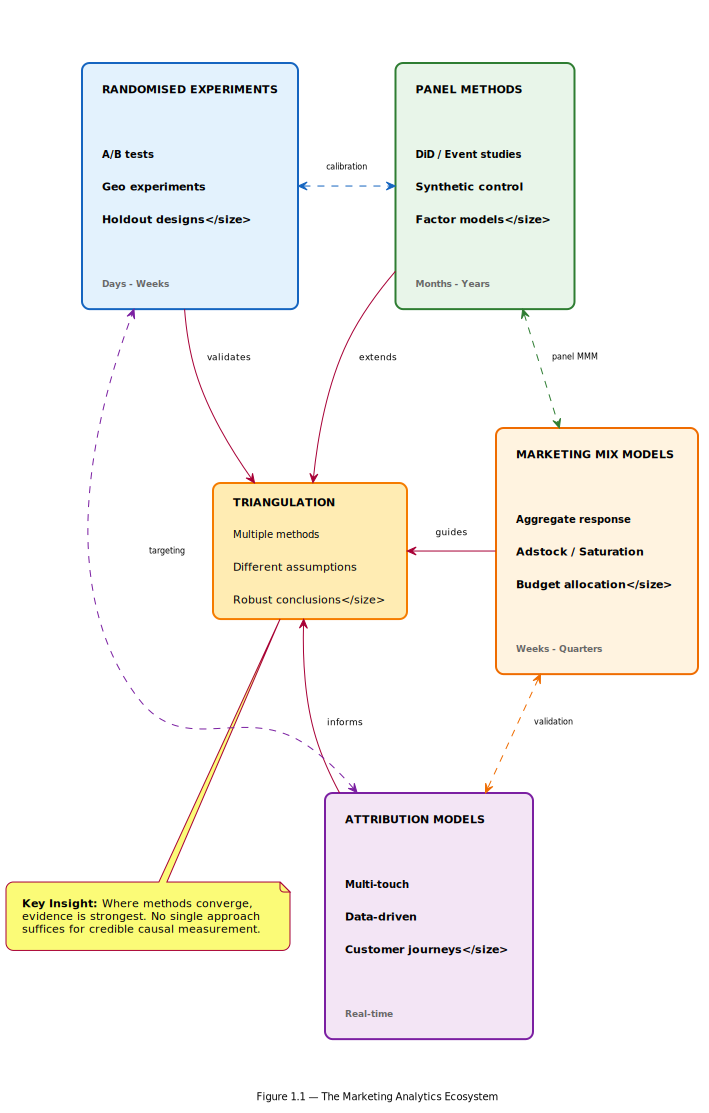
\includegraphics[width=0.7\textwidth]{images/ecosystem.png}
\caption{The Marketing Analytics Ecosystem: Experiments, Panels, MMM, and Attribution}
\label{fig:ecosystem}
\end{figure}

MMM and panel methods are not mutually exclusive. Many workflows combine MMM-style transforms (adstock, saturation) with design-based identification in panels (DiD, SC, IV). Panel MMMs are natural when you have multi-market or store-level data, and design-based logic strengthens identification. Factor-augmented panels (Chapters~\ref{ch:factor}, \ref{ch:advanced-matrix}) and instrumental variables (Chapters~\ref{ch:frameworks}, \ref{ch:inference}) further bridge modelling and design.

Today's methods did not emerge fully formed. They reflect decades of intellectual development responding to new data, computational capabilities, and substantive challenges. Figure~\ref{fig:timeline} depicts this evolution.

The 1980s and 1990s were dominated by two-way fixed effects and random effects models controlling for time-invariant unobservables. The design-based revolution of the 2000s brought synthetic control methods \citep{abadie2003economic,abadie2010synthetic} and renewed focus on difference-in-differences with explicit parallel trends assumptions. The late 2010s saw the discovery of negative weighting in staggered TWFE designs \citep{goodman2021difference,dechaisemartin2020two}, sparking heterogeneity-robust estimators that aggregate cohort-specific effects without using previously treated units as controls.

Recognition that parallel trends in levels may be too restrictive motivated synthetic control methods matching on pre-treatment trajectories. The proliferation of high-dimensional data---rich customer covariates, detailed competitor actions, granular geographic variation---prompted machine learning integration for flexible control and heterogeneous effect estimation. This timeline demonstrates the iterative, self-correcting nature of methodological progress. Today's methods will be refined or replaced as new challenges arise. The marketing applications driving this book---loyalty programmes, advertising campaigns, platform expansions---have played an important role, providing both motivation for new methods and empirical testing grounds where strengths and limitations can be identified.

\begin{figure}[htbp]
\centering
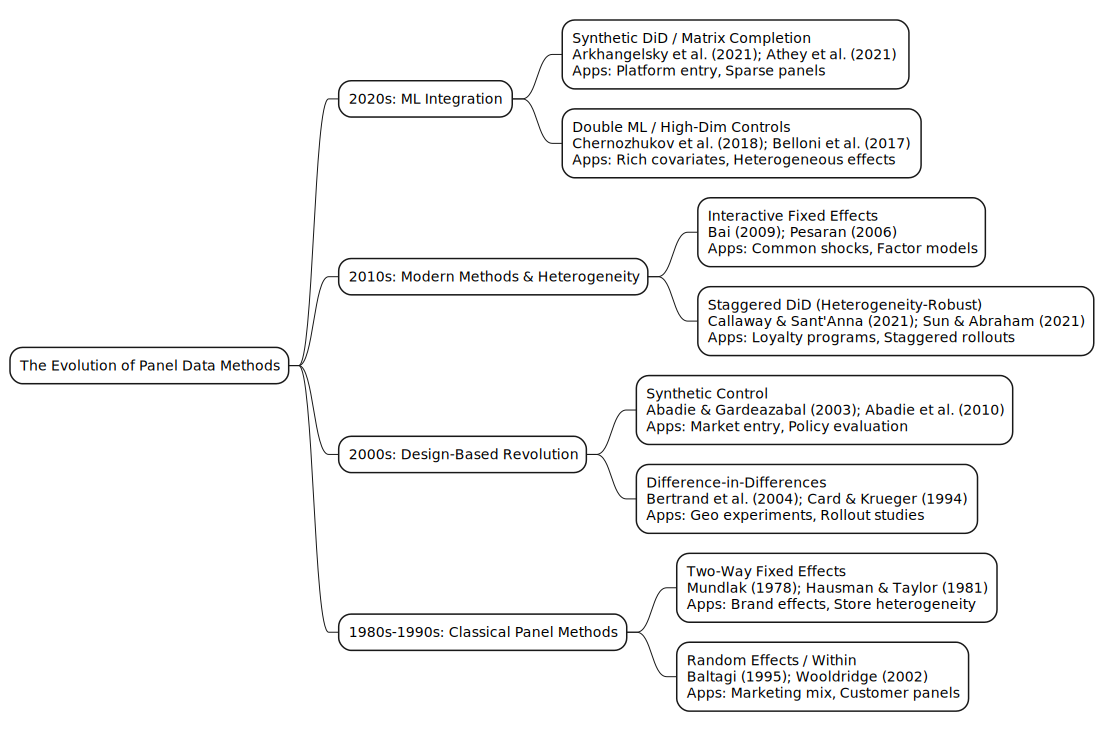
\includegraphics[width=0.95\textwidth]{images/timeline.png}
\caption{Timeline of Panel Data Methods: From TWFE to Modern Heterogeneity-Robust and ML-Integrated Approaches}
\label{fig:timeline}
\end{figure}

The aims of this book grew out of several converging developments rather than a single influence. A sequence of methodological breakthroughs in causal inference for panel data, together with a rapidly expanding applied literature, has made it possible to study marketing interventions with far greater rigour than traditional time-series or attribution approaches allow. At the same time, much of the marketing analytics discourse has drifted toward predictive machine learning, often with only loose connections to identification and design. This book attempts to recentre the discussion on causal structure and research design, while still drawing on modern tools where they genuinely strengthen empirical work.

Within this landscape, \citet{arkhangelsky2024causal} provides a rigorous synthesis of modern causal panel methods. We build on similar foundations but with different emphasis: marketing-specific issues---attribution challenges, algorithmic confounding, applications in loyalty programmes and advertising---that receive limited attention in econometrics texts; machine learning as a supporting tool for identification rather than stand-alone prediction; and a practitioner orientation emphasising intuition, diagnostics, and method selection over formal proofs, while maintaining technical precision in assumptions and identification.

\section{Motivating Examples: Three Marketing Challenges}
\label{sec:motivating-examples}

To ground the abstract discussion of panel methods in concrete marketing problems, we consider three hypothetical scenarios that motivate the methods developed in subsequent chapters. Each scenario illustrates a distinct set of challenges and maps to a different constellation of panel data tools. While stylised, these examples reflect real measurement challenges practitioners face.

\subsection*{Example 1: Evaluating a Loyalty Programme with Staggered Rollout}

Consider a hypothetical retail chain operating 500 stores across multiple regions with three years of quarterly sales data. To increase customer retention and lifetime value, the chain launches a loyalty programme offering points for purchases, redeemable for future discounts. Rather than rolling out the programme simultaneously, the firm adopts a phased approach: 100 stores in year one, an additional 200 in year two, 150 more in year three. The remaining 50 stores — primarily small, remote locations — never receive the programme, serving as controls.

The staggered rollout reflects operational constraints and strategic considerations. Early adopters tend to be larger stores in high-income areas where management anticipates strong programme uptake. Later adopters include stores in more competitive markets, where the firm hopes the programme will help defend market share. This non-random assignment creates selection bias: programme stores differ systematically from non-programme stores in ways that affect sales even absent the programme. Simply comparing sales in programme stores to sales in non-programme stores would conflate the programme effect with these pre-existing differences.

The evaluation faces additional complications. Spillovers loom large: customers who join may refer friends or family, creating positive peer effects, while customers from nearby non-programme stores may switch to programme stores to earn rewards. The programme effect is unlikely to be immediate or constant — initial enrolment may be slow, habit formation takes time, and switching costs build gradually as customers accumulate points. There may even be anticipation effects if rumours of the impending launch spread beforehand. The effect likely varies across store types, with affluent, low-competition neighbourhoods seeing different responses than saturated urban markets where customers already have multiple loyalty options.

This scenario maps naturally to modern panel data methods. The staggered rollout calls for difference-in-differences estimators that accommodate heterogeneous adoption timing (Chapter \ref{ch:did}). Event-study specifications (Chapter \ref{ch:event}) plot treatment effects over time and enable pre-trend tests. Spillover models (Chapter \ref{ch:spillovers}) estimate geographic externalities. Causal forests (Chapter \ref{ch:ml-nuisance}) uncover heterogeneity across store types. Chapters \ref{ch:design-diagnostics} and \ref{ch:inference} develop the diagnostic workflow including placebo tests, leave-one-out analyses, and sensitivity analyses.

What might such an analysis reveal? In this hypothetical case, suppose the estimated average treatment effect were eight per cent across all programme stores and quarters. This aggregate effect would mask important dynamics: an initial effect of just two per cent in the first quarter post-launch, growing to eight per cent after four quarters and stabilising thereafter. Spillovers might be positive but modest — sales in non-programme stores within five kilometres of a programme store rising by two per cent, suggesting word-of-mouth effects. Heterogeneity analysis might reveal effects concentrated in high-income, low-competition areas (twelve per cent increase) with near-zero effects in saturated urban markets. These richer insights would guide not just whether to expand the programme, but where to expand it and how to manage expectations about the timeline for seeing results.

\subsection*{Example 2: Measuring Television Advertising Carryover in the Digital Age}

Suppose a consumer packaged goods brand seeks to understand the causal effect of TV advertising on sales, accounting for carryover effects and digital channel interactions. The hypothetical data consist of weekly observations for 50 designated market areas over 100 weeks, capturing gross rating points (GRPs), online search volume, social media mentions, and sales. The advertising agency varies TV spending strategically — higher during product launches, in markets with active competitors, and when prior sales trends suggest rising demand.

This endogeneity of TV spending is the first challenge. Markets that receive heavy TV advertising in a given week may be fundamentally different in that week from markets that receive little advertising. Even if we control for time-invariant market characteristics with fixed effects, time-varying confounders -- competitor actions, local economic shocks, seasonal patterns -- may drive both the advertising decision and sales, creating spurious correlation. A second challenge is carryover: TV advertising effects do not instantaneously materialise and vanish. Some viewers respond immediately by searching online or visiting a store. Others store the information and act days or weeks later. Brand awareness accumulates over repeated exposures and decays gradually in the absence of advertising. Specifying the functional form of this carryover is non-trivial and has been the subject of extensive research in the marketing mix modelling tradition. Third, cross-channel effects complicate the picture. TV advertising may increase online search, which in turn increases sales. If we estimate the total effect of TV on sales, we capture both the direct effect and the indirect effect mediated through search. But if we control for search in a regression, we may block the causal pathway and underestimate the TV effect. Understanding these mediated effects is substantively important but econometrically delicate. Fourth, measurement issues abound: Nielsen television ratings are based on panels that may not perfectly represent the full population, sales data are aggregated from retail scanner panels with their own coverage gaps, and seasonal effects (holidays, weather, major events) create non-stationarity that must be disentangled from treatment effects.

Several panel methods suit this scenario. Synthetic control methods (Chapters \ref{ch:sc}, \ref{ch:generalized-sc}) construct bespoke control groups for treated markets. Distributed lag models (Chapter \ref{ch:dynamics}) parameterise carryover structure. High-dimensional control methods (Chapter \ref{ch:high-dim}) handle many potential confounders through data-driven variable selection. Chapters \ref{ch:inference} and \ref{ch:design-diagnostics} cover cluster-robust inference, placebo tests, and sensitivity analyses for carryover assumptions.

In a hypothetical analysis, TV advertising might increase sales by five per cent in the campaign week, with a three-week half-life. Online search could mediate roughly forty per cent of the total effect, with TV driving search and search driving sales. Competitor advertising might partially offset the own-brand effect — reducing it by twenty per cent when competitors simultaneously increase spending. Carryover could prove stronger for emotional appeals than informational appeals, consistent with theories of memory and persuasion. Such insights would inform budget allocation, creative strategy, and competitive response.

\subsection*{Example 3: Platform Market Entry and Competitive Dynamics}

Consider a hypothetical food delivery platform (stylised examples include DoorDash, Deliveroo, or Uber Eats) entering 30 new cities over two years. The firm observes monthly restaurant revenues in both entry cities and comparison cities without platform entry. The data span 50 cities and 36 months, creating a panel with staggered treatment timing. The firm seeks to estimate the causal effect of platform entry on restaurant revenues, accounting for competitive dynamics and general equilibrium effects.

Several challenges complicate the analysis. Each city is unique, so finding exact matches for treated cities among the control cities is impossible. The firm selects entry cities based on market size, demographics, competitive landscape, and regulations. This introduces selection bias. Entry occurs at different times for different cities, with larger, more attractive markets entered first. Once the platform enters a city, incumbent platforms (competitors already operating in that city) may respond by lowering commissions, increasing marketing, or improving service quality, mitigating the treatment effect and inducing competitive spillovers. Moreover, platform entry affects not just the restaurants that join the platform but potentially the entire restaurant ecosystem: consumers may dine out more frequently (category expansion), delivery drivers shift labour supply, and even restaurants that do not join the platform may see changes in foot traffic or delivery orders through third-party services.

This scenario motivates several panel methods. Synthetic control (Chapter \ref{ch:sc}) constructs control cities from weighted averages of never-treated cities, with inference via permutation tests. Synthetic difference-in-differences (Chapter \ref{ch:generalized-sc}) combines unit and time weights for staggered entry settings. Factor models (Chapter \ref{ch:factor}) handle unobserved common shocks affecting all cities. Spillover models (Chapter \ref{ch:spillovers}) quantify competitive responses. We develop these methods and their diagnostics in Chapters \ref{ch:did} through \ref{ch:spillovers}.

Hypothetical findings might show platform entry increasing restaurant revenues by fifteen per cent on average, with substantial heterogeneity. Small, independent restaurants could see twenty-five per cent gains from expanded reach, while chains with established delivery operations might see only five per cent gains. The competitive response from incumbent platforms could offset the effect by roughly thirty per cent in markets where incumbents lower commissions or increase promotions. General equilibrium effects might be positive — the category expanding as consumers order more frequently — suggesting platform entry creates value rather than merely redistributing it, with implications for regulatory policy and market structure.

These three hypothetical examples illustrate the range of marketing questions panel data methods can address — selection bias, dynamics, spillovers, heterogeneity, measurement error, competitive interactions. Each will recur in subsequent chapters as we develop the technical methods and diagnostic workflows for credible causal inference.

\section{The Two Cultures of Marketing Analytics}
\label{sec:two-cultures}

In a celebrated paper, statistician Leo Breiman distinguished two cultures in statistical modelling. The first, ``data modelling'', builds explicit probabilistic models and estimates parameters under strong assumptions about functional form. The second, ``algorithmic modelling'', treats the underlying mechanism as unknown and focuses on predictive accuracy through flexible, data-adaptive algorithms. Breiman argued that statistics had long overemphasised the first culture and neglected the second, missing opportunities to harness the power of machine learning for prediction.

This dichotomy, while influential, has been critiqued as overly stark. As Andrew Gelman and others have argued, good statistical practice has always blended elements of both cultures. Data modellers routinely check their models' predictive performance through cross-validation and other checks. Algorithmic modellers increasingly seek interpretability through tools like SHAP values and partial dependence plots. The real tension is not between prediction and understanding, but between strong parametric assumptions and flexible, data-adaptive methods. Crucially, neither culture, as originally framed, directly addresses the central challenge of marketing analytics: moving from prediction or association to *causal* inference.

Marketing analytics today reflects this tension. The rise of digital platforms has fuelled an explosion in predictive modelling -- churn prediction, recommendation engines, bid optimisation. These models excel at forecasting outcomes *within* the existing system. Yet when organisations face strategic decisions -- should we launch this loyalty programme? will this price change increase long-run revenue? -- prediction alone is insufficient. We need causal inference. This is where panel data methods, grounded in quasi-experimental design but augmented with modern machine learning, offer a path forward.

Modern panel data methods for causal inference represent a synthesis -- or perhaps a third culture. They borrow the flexibility of algorithmic modelling to handle high-dimensional confounders and estimate heterogeneous treatment effects. Yet they retain the discipline of data modelling by making explicit assumptions about the causal structure, such as parallel trends or unconfoundedness, and subjecting those assumptions to diagnostic tests. Methods like Double Machine Learning epitomise this synthesis. Machine learning algorithms estimate nuisance functions with minimal parametric assumptions, while design-based identification strategies ensure that the final causal estimate is robust. This approach prioritises causal validity over pure predictive accuracy, but it uses the tools of both cultures to achieve it.

Our approach to reasoning through models is pragmatic. We do not seek a single, true model that perfectly captures the data-generating process -- such a model does not exist, and even if it did, we could not be certain we had found it. Instead, we embrace a workflow that combines four elements. We begin by articulating the identification assumptions -- parallel trends, conditional independence, factor structure, no spillovers -- required for a causal interpretation of our estimates. We then apply an estimator that implements the identification strategy, whether it be difference-in-differences, synthetic control, interactive fixed effects, or a doubly robust machine learning method. Having obtained estimates, we conduct an extensive battery of diagnostics -- pre-trend tests, placebo tests, balance checks, leave-one-out robustness, covariate balance, specification curves -- to assess whether the assumptions are plausible and whether the results are sensitive to modelling choices. Finally, we quantify through sensitivity analysis how large a violation of the key assumptions would need to be to overturn our conclusions, acknowledging that assumptions are approximations rather than exact truths. This workflow embodies the synthesis of cultures: flexible tools deployed within a disciplined causal framework.

\section{Strategic Dynamics and Marketing Phenomena}
\label{sec:strategic-dynamics}

Marketing phenomena often exhibit dynamics and strategic interactions that panel data methods are well positioned to study. We consider six domains where panel methods illuminate questions of central interest to marketing strategists, grouping them loosely into timing and entry questions, advertising and investment effectiveness, and competitive interactions.

Market entry and competitive timing raise fundamental strategic questions. When should a firm enter a new market? What advantages accrue to pioneers versus fast followers? How do entry timing and order affect long-run market shares and profitability? These questions have occupied marketing scholars for decades, with some arguing that first movers enjoy enduring advantages from consumer lock-in and brand recognition, while others contend that later entrants can free-ride on pioneers' investments in consumer education and avoid early mistakes. Panel data tracking firms' entry across multiple markets and over time permit difference-in-differences analyses that compare outcomes for early versus late entrants, controlling for time-invariant market characteristics and common temporal shocks. If a firm expands into new cities sequentially, the staggered rollout enables within-firm comparisons that hold firm-specific factors constant, isolating the effect of entry timing net of firm quality.

Related to entry is the question of diffusion and takeoff. Innovations diffuse through populations at varying speeds. When does an innovation experience takeoff -- the transition from slow initial adoption to rapid growth? Panel data on product sales or adoption rates across multiple markets and time periods enable models that relate diffusion speed to market characteristics, competitive intensity, and marketing actions. Methods from survival analysis and hazard modelling, combined with panel structures, allow researchers to estimate the time to takeoff as a function of covariates, accounting for unobserved market heterogeneity through fixed effects or frailties.

Advertising effectiveness raises distinct challenges. How effective is advertising in driving sales? What is the lag structure of advertising effects -- how long does it take for an advertising campaign to exert its full influence, and how quickly does the effect decay? Do diminishing returns set in at high spending levels? Panel data with variation in advertising across markets and time, combined with distributed lag models or dynamic panel specifications, enable estimation of advertising elasticities, carryover parameters, and saturation thresholds. Synthetic control methods provide a complementary approach by constructing counterfactual markets that resemble treated markets in the pre-campaign period and comparing post-campaign outcomes.

Shareholders care whether marketing investments -- new product launches, brand repositioning, advertising campaigns -- create value. Event-study methodologies, applied to panel data on stock prices and firm-level events, estimate abnormal returns in the days or weeks following an announcement or event, controlling for market-wide movements and industry trends. By pooling multiple events across firms and time, panel event studies improve statistical power and allow researchers to explore heterogeneity in stock market reactions as a function of firm characteristics, competitive context, and event features.

The digital era has elevated the importance of user-generated content and online reviews. How does online chatter -- reviews on Yelp or Amazon, social media mentions, sentiment in discussion forums -- affect sales and firm value? Panel data tracking product-level sales and review volumes enable quasi-experimental designs that exploit plausibly exogenous variation in online content. If an influential reviewer's coverage of a product is driven by idiosyncratic timing rather than the product's underlying quality trends, the timing of the review can serve as a quasi-experiment. Vector autoregression models fitted to panel data can trace the dynamic feedback between chatter and outcomes, distinguishing whether chatter predicts future sales (a signal of quality) or whether sales drive chatter (a mechanical relationship).

Finally, competitive dynamics demand attention. How do competitors respond to a firm's actions? If one firm cuts price, launches a product, or increases advertising, do rivals retaliate, accommodate, or ignore? Panel data on competitor actions and outcomes, combined with models of strategic interaction, allow researchers to estimate reaction functions that describe how one firm's choices depend on rivals' past choices. Difference-in-differences and synthetic control methods can estimate the causal effect of one firm's action on rivals' outcomes, quantifying competitive spillovers and market equilibrium effects.

In each of these domains, classical marketing models have provided descriptive insights. Bass diffusion curves characterise the S-shaped adoption pattern but do not identify the causal effect of marketing interventions on diffusion speed. Koyck and polynomial distributed lag models describe the time path of advertising effects but do not resolve endogeneity or establish that the correlations are causal. Vector autoregression models trace the joint dynamics of marketing inputs and outputs but typically do not distinguish causal relationships from correlations induced by common shocks. Modern panel data methods add a causal lens to these descriptive models by specifying identification strategies that justify moving from association to causation. A Bass model predicts the adoption curve under the status quo, but a difference-in-differences analysis estimates how a subsidy or marketing campaign shifts the curve. A vector autoregression shows that advertising and sales co-move, but a synthetic control analysis estimates the causal effect of an increase in advertising. Panel methods do not replace classical models; they complement them by providing a framework for causal inference.

\section{The Causal Revolution in Marketing}
\label{sec:causal-revolution}

Marketing is shifting from metrics-focused dashboards to mechanism-focused causal analysis. For much of the digital era, organisations measured success using intermediate metrics---impressions, clicks, page views, ad recall---that serve as proxies for business outcomes. These metrics help optimise within a fixed strategic framework: if clicks predict sales, we can tune bidding to maximise clicks per dollar. But when used to assess strategic changes, intermediate metrics mislead. A campaign generating many clicks may not drive incremental sales if those clicks come from users who would have bought anyway. A loyalty programme that raises repeat purchase rates may not increase profits if it merely shifts purchases forward in time rather than expanding total consumption.

The incrementality problem has prompted major platforms to build causal measurement tools. Meta's Conversion Lift uses an intent-to-treat design: users are randomly assigned to a holdout group, blocked from seeing the campaign's ads, or to a treatment group eligible for delivery. Conversion rates are compared to estimate incremental lift. Within the treatment group, however, the platform's targeting algorithm still determines who actually sees ads---randomisation occurs at the eligibility level, not exposure level. Google's Geo-Experiments randomly vary advertising intensity across geographic areas to estimate aggregate regional effects. Amazon's Brand Lift studies use similar holdout designs for awareness and intent. These tools represent genuine advances over last-touch attribution, but they share common limitations: proprietary implementations that researchers cannot audit, aggregated outputs that obscure heterogeneity and dynamics, and platform-specific designs that prevent cross-channel comparison. \cite{lewis2015unfavorable} quantify a related problem: even well-designed digital experiments often lack statistical power to detect economically meaningful effects, because per-user revenue variance swamps treatment effects.

Panel data methods supplement platform tools by offering transparent, reproducible, and flexible approaches to causal inference. The methods in this book apply to any panel dataset, not just those accessible via platform interfaces. They incorporate external data---competitor actions, macroeconomic conditions, offline behaviour---that platforms do not observe. They estimate long-run effects by tracking outcomes over months or years rather than the weeks typical of platform experiments. Spillovers, dynamics, and heterogeneity can be modelled explicitly and diagnosed rigorously. Assumptions are stated, tested, and debated rather than hidden inside proprietary code.

This shift toward causal rigour reflects a broader intellectual movement. \cite{angrist2010credibility} labelled it the credibility revolution: economists began emphasising research designs that approximate randomised experiments---instrumental variables exploiting exogenous shocks, regression discontinuity designs using threshold-based assignment, and difference-in-differences comparing treated and control units before and after intervention. Combined with richer administrative data, these methods raised the evidential bar. Cross-sectional regressions with long covariate lists gave way to designs grounded in institutional detail, policy discontinuities, and natural experiments that generate credible counterfactuals.

Marketing scholarship has adopted these lessons more slowly than labour economics or public finance, but the trajectory is clear. Leading journals now routinely publish quasi-experimental studies, and methodological sophistication in causal inference is increasingly expected. This book accelerates adoption by providing a rigorous yet accessible treatment tailored to marketing's distinctive data structures and substantive questions.

The challenges ahead are formidable. Platform algorithms now decide which users see which ads, which products rank in search, and what prices appear to different customers. This algorithmic intermediation creates confounding by design: exposures depend on predicted responses, rankings on past clicks, prices on inferred willingness to pay. Causal inference must confront data-generating processes in which treatments are functions of predicted outcomes.

Privacy constraints compound the difficulty. Deprecation of third-party cookies, Apple's App Tracking Transparency, and GDPR limit cross-device and cross-platform tracking, producing missing data and measurement error. Panel methods must adapt: aggregate or differentially private data, partial identification under incomplete information, and triangulation across imperfect sources all become necessary.

Nonstationarity poses a third challenge. Consumer preferences shift, technologies emerge, competitors enter and exit, macroeconomic shocks disrupt demand. Panel methods often assume some stationarity---parallel trends, time-invariant effects, stable factor loadings---that may fail during upheaval. Methods for structural breaks, time-varying parameters, and regime changes remain active research frontiers.

Interference grows more complex in networked platforms where users connect to many others, and in competitive markets where firms react strategically in real time. Partial interference assumptions---spillovers only within clusters, decay with geographic distance---may prove inadequate for modern marketing ecosystems. Developing tractable yet realistic interference models is an open problem.

These challenges, however, create opportunities. The same platforms that complicate inference through algorithmic targeting generate unprecedented granular data: clickstreams, location traces, social graphs, review text. Computational advances permit estimation of complex models at scale. Machine learning contributes not through prediction per se, but through flexible estimation of nuisance functions---propensity scores, outcome models, latent factors---that sharpen causal estimates. Double machine learning \citep{chernozhukov2018double} and causal forests \citep{wager2018estimation} exemplify this integration, using regularised learners to handle high-dimensional confounding while preserving valid inference on treatment effects.

The methods developed in this book help readers navigate this landscape. Whether evaluating a loyalty programme, measuring advertising effectiveness, quantifying competitive dynamics, or assessing platform design changes, causal panel methods provide a disciplined framework for moving from correlation to cause. Causal claims remain provisional---grounded in approximations, not certainties. But with rigorous methods, transparent diagnostics, and systematic sensitivity analysis, we can distinguish interpretations that deserve credibility from those that do not.

\begin{table}[htbp]
\begin{tighttable}
\centering
\caption{Overview of Three Motivating Examples}
\label{tab:motivating-examples}
\begin{tabularx}{\textwidth}{Y Y Y Y}
\toprule
\textbf{Example} & \textbf{Challenges} & \textbf{Methods} & \textbf{Key Insights} \\
\midrule
Loyalty Programme Rollout & Selection bias, spillovers, dynamics, heterogeneity & Staggered DiD (Ch \ref{ch:did}), event studies (Ch \ref{ch:event}), spillover models (Ch \ref{ch:spillovers}), causal forests (Ch \ref{ch:ml-nuisance}) & 8\% avg effect, growing over time; spillovers +2\%; heterogeneous (12\% high-income, 0\% saturated markets) \\
\addlinespace
TV Advertising Carryover & Endogeneity, carryover, mediation, seasonality & Synthetic control (Ch \ref{ch:sc}), distributed lags (Ch \ref{ch:dynamics}), lasso (Ch \ref{ch:high-dim}), robust inference (Ch \ref{ch:inference}) & 5\% immediate effect, 3-week half-life; 40\% mediated via search; competitor response -20\% \\
\addlinespace
Platform Entry & Unique units, staggered timing, competition, general equilibrium & SC (Ch \ref{ch:sc}), SDID (Ch \ref{ch:generalized-sc}), factor models (Ch \ref{ch:factor}), spillover models (Ch \ref{ch:spillovers}) & 15\% avg effect; 25\% for small restaurants, 5\% chains; competitive response -30\%; category expansion (positive-sum) \\
\bottomrule
\end{tabularx}
\end{tighttable}
\end{table}

\section{Why Marketing Panel Data is Different}
\label{sec:why-marketing}

A reasonable question for any reader of this monograph is: \textit{Why do we need a specialised book on panel data for marketing?} Excellent textbooks already exist for biostatistics, financial econometrics, and labour economics. Can the marketing analyst not simply adopt the tools of the clinical trial or the asset pricing model?

The answer is that marketing data differs structurally from standard medical and financial data in ways that often break standard estimators. While marketing shares some DNA with modern epidemiology (observational studies of contagion and policy), it is distinct from the randomised clinical trials that dominate biostatistics. The same features that make marketing data rich---strategic behaviour, social connectivity, and high-frequency measurement---introduce specific violations of the assumptions that underpin traditional methods. Four structural differences define the challenge.

\subsection*{1. The Targeting Bias (Endogeneity by Design)}
In clinical trials, treatment is randomised. In labour economics, treatment (e.g., a minimum wage hike) is often exogenous to the individual worker. In marketing, treatment is \textbf{strategic and endogenous}. Firms actively target advertising, coupons, and sales calls to customers who are \textit{most likely to buy} (retargeting) or \textit{most likely to churn} (retention).

Standard estimators like simple Difference-in-Differences (DID) do not just yield biased estimates in this setting; they often get the sign wrong. A naive analysis of a retargeting campaign will show that treated users purchase at vastly higher rates than control users. This is not the effect of the ad; it is the cause of the targeting. Disentangling the \textit{targeting policy} from the \textit{treatment effect} requires methods that go beyond controlling for fixed attributes, such as Negative Controls, Double Machine Learning (Chapter~\ref{ch:ml-nuisance}), and Synthetic Control methods that match on pre-treatment trajectories (Chapter~\ref{ch:sc}).

\subsection*{2. Interference is the Norm, Not the Exception}
The Stable Unit Treatment Value Assumption (SUTVA)---that one unit's outcome depends only on its own treatment---is a reasonable approximation in clinical trials (my taking aspirin does not cure your headache). In marketing, it is routinely violated, much like in infectious disease epidemiology. Social interference arises when a customer's purchase makes their friends more likely to buy the same product through network effects and contagion. Spatial interference occurs when a television ad in one designated market area spills over into adjacent DMAs. Competitive interference emerges when one firm's price cut prompts competitors to respond, altering the equilibrium outcome for everyone. Standard panel methods that assume independence between units will fail to identify the true effect. Marketing analytics requires Spatial Error Models, Network Interference designs, and cluster-randomised experiments (Chapter~\ref{ch:spillovers}) to account for the fact that the "control group" is constantly contaminated by the "treatment group."

\subsection*{3. The "Fat and Long" Data Structure}
Clinical datasets typically feature small $N$ and short $T$ (100 patients observed 3 times). Financial datasets feature small $N$ and very long $T$ (500 stocks observed daily for 20 years). Marketing data is unique: we often observe \textbf{massive $N$ and moderate $T$}. A retailer may track 10 million customers over 52 weeks. Moreover, the data is \textbf{sparse}: most customers do not buy in most weeks.

This structure renders traditional time-series methods (GARCH, Cointegration) and traditional biostatistical methods (Mixed Models) computationally infeasible or statistically inefficient. It is, however, the ideal structure for \textbf{Matrix Completion} and \textbf{Factor Models} (Chapters~\ref{ch:factor} and \ref{ch:advanced-matrix}). These methods leverage the low-rank structure of consumer behaviour---the fact that millions of diverse customers share a small number of underlying latent preferences---to impute counterfactuals with high precision.

\subsection*{4. Complex Dynamics: Adstock and Wear-out}
Financial markets are often modelled as efficient, incorporating new information instantly. Marketing effects, by contrast, exhibit complex lag structures. An ad seen today may influence a purchase next week (Adstock/Memory), but seeing the same ad ten times may reduce its effectiveness (Wear-out/Non-monotonicity). Habit formation creates state dependence, where past purchases influence future probability of purchase.

Disentangling \textit{incremental lift} from \textit{carryover effects} requires Distributed Lag Models and Event Studies (Chapters~\ref{ch:event} and \ref{ch:dynamics}) that are specifically tuned to the "stock and flow" nature of marketing goodwill.

Table~\ref{tab:domain-comparison} summarises these structural distinctions. While we draw inspiration from epidemiology for interference and observational inference, the combination of strategic targeting and massive sparse matrices makes marketing analytics a distinct methodological field.

\begin{table}[t]
\centering
\begin{tighttable}
\caption{Structural Differences Across Domains}
\label{tab:domain-comparison}
\begin{tabularx}{\textwidth}{lXXX}
\toprule
\textbf{Feature} & \textbf{Clinical / Biostats} & \textbf{Financial Econometrics} & \textbf{Marketing Analytics} \\
\midrule
\textbf{Primary Goal} & Efficacy / Safety & Risk / Forecasting & \textbf{Incrementality / ROAS} \\
\addlinespace
\textbf{Assignment} & Randomised (RCT) & Systemic / Exogenous & \textbf{Strategic (Targeting)} \\
\addlinespace
\textbf{Interference} & Rare (except Vaccines) & Market-wide Equilibrium & \textbf{High (Social / Spatial)} \\
\addlinespace
\textbf{Data Shape} & Small $N$, Short $T$ & Small $N$, Long $T$ & \textbf{Large $N$, Moderate $T$} \\
\addlinespace
\textbf{Sparsity} & Low (Complete records) & Low (Continuous trading) & \textbf{High (Infrequent purchase)} \\
\addlinespace
\textbf{Key Method} & Survival / Mixed Models & Time Series / GARCH & \textbf{Synthetic Control / Matrix Factorization} \\
\bottomrule
\end{tabularx}
\end{tighttable}
\end{table}
\section{Roadmap of the Book}
\label{sec:roadmap}

This book is organised into eight Parts that build from foundational concepts through core methodologies to inference, diagnostics, and applications.

\textbf{Part I: Foundations} (Chapters 1--3) establishes the causal framework and panel notation. Chapter 2 formalises potential outcomes for panel data, distinguishing contemporaneous from path-dependent treatments, and defines key estimands. Chapter 3 contrasts randomised experiments with quasi-experimental designs including geo-experiments, switchback tests, and phased rollouts.

\textbf{Part II: Differences-in-Differences and Event Studies} (Chapters \ref{ch:did}--\ref{ch:event}) develops canonical and staggered DiD designs. We present modern heterogeneity-robust estimators that avoid negative weighting and trace dynamic treatment effects through event-study specifications with pre-trend tests.

\textbf{Part III: Synthetic Controls and Hybrid Methods} (Chapters \ref{ch:sc}--\ref{ch:generalized-sc}) introduces synthetic control for settings where pre-treatment fit substitutes for parallel trends. Chapter \ref{ch:generalized-sc} covers hybrid approaches including synthetic DiD and augmented synthetic control with doubly robust estimation.

\textbf{Part IV: Factor Models and Matrix Methods} (Chapters \ref{ch:factor}--\ref{ch:advanced-matrix}) exploits low-rank structure in panel data. Interactive fixed effects capture common time-varying shocks with unit-specific loadings. Matrix completion methods handle missing data and high-dimensional settings through nuclear-norm regularisation.

\textbf{Part V: Dynamics and Spillovers} (Chapters \ref{ch:dynamics}--\ref{ch:spillovers}) addresses treatment path dependence through distributed lag and adstock models. Chapter \ref{ch:spillovers} tackles SUTVA violations from network, geographic, and competitive spillovers using spatial econometrics and partial identification.

\textbf{Part VI: Machine Learning Integration} (Chapters \ref{ch:ml-nuisance}--\ref{ch:continuous}) introduces double/debiased machine learning for nuisance function estimation with Neyman orthogonalisation. Causal forests estimate heterogeneous effects. Lasso and regularisation handle high-dimensional confounders. Extensions cover continuous treatments, dose-response functions, and quantile effects.

\textbf{Part VII: Validity and Inference} (Chapters \ref{ch:threats}--\ref{ch:design-diagnostics}) catalogues marketing-specific threats including algorithmic confounding and platform metric misalignment. Inference tools include cluster-robust standard errors, bootstrap procedures, randomisation inference, and multiple testing adjustments. Diagnostic workflows encompass placebo tests, balance checks, and specification curves.

\textbf{Part VIII: Applications and Future Directions} (Chapters \ref{ch:applications}--\ref{ch:outlook}) synthesises methods through integrated case studies combining DiD, synthetic control, event studies, and causal forests. Chapter \ref{ch:data-measurement} examines scanner data, platform logs, and measurement challenges including privacy regulations. Chapter \ref{ch:outlook} identifies open problems in interference, nonstationarity, real-time optimisation, and method selection frameworks.

Each chapter follows a consistent structure: motivation, identification assumptions, estimation, inference, diagnostics, and marketing applications.

% Chapter 2
\chapter{Causal Frameworks and Panel Notation}
\label{ch:frameworks}

This chapter develops the causal framework and panel notation that underpin all subsequent analysis. We formalise potential outcomes notation for panel data, including dynamic treatment paths, and define core estimands such as average treatment effects and event-time effects that recur throughout the book. We distinguish common data configurations -- proper panels, grouped repeated cross-sections, and row-column exchangeable data -- and classify assignment mechanisms that drive identification choices. Finally, we review basic regression mechanics and inference issues specific to panel settings. These foundations equip you with the conceptual vocabulary and technical prerequisites for the methods developed in later chapters.

\noindent\textbf{Learning objectives.} You will learn how to formalise potential outcomes for panels, define core estimands (ATE, ATT, event-time effects), classify data structures and assignment mechanisms, understand when basic regression tools succeed or fail, and map your data to appropriate methods via the crosswalk framework.

\section{Potential Outcomes for Panels}
\label{sec:potential-outcomes-panels}

The measurement challenges outlined in Chapter 1 --- endogeneity, dynamics, spillovers --- demand a precise language for counterfactual comparisons. Without such a language, we cannot state clearly what we seek to learn, let alone estimate it credibly.

The potential outcomes framework provides this foundation. Rubin formalised the framework \citet{rubin1974estimating}, and empirical economists now use it widely \citet{angrist2010credibility}. This section sets out the notation and assumptions that underpin the estimators developed in subsequent chapters, with particular attention to the complications that repeated observations introduce.

We observe data on $N$ units indexed by $i = 1, \ldots, N$ over $T$ periods indexed by $t = 1, \ldots, T$. For each unit and period, we observe an outcome $Y_{it}$ and a treatment status $W_{it}$. In the simplest case, $W_{it}$ is binary: it takes the value one if unit $i$ is treated in period $t$ and zero otherwise. The treatment may be an intervention applied to the unit --- a store receiving a loyalty programme, a market exposed to an advertising campaign, a platform entering a city --- or it may represent a continuous intensity variable such as advertising expenditure or promotional discount depth. For now, we focus on the binary case. We return to continuous and multivalued treatments in Chapter~\ref{ch:continuous}.

The potential outcomes framework posits that for each unit $i$ and period $t$, there exist multiple potential outcomes corresponding to different treatment states. In the binary case, we imagine two potential outcomes: $Y_{it}(0)$, the outcome that would be realised if unit $i$ were not treated in period $t$, and $Y_{it}(1)$, the outcome that would be realised if unit $i$ were treated in period $t$. The treatment assignment links the observed outcome $Y_{it}$ to these potential outcomes:
\[
Y_{it} = W_{it} Y_{it}(1) + (1 - W_{it}) Y_{it}(0).
\]
This switching equation clarifies that we observe only one potential outcome for each unit and period. We never observe the counterfactual outcome --- $Y_{it}(0)$ for treated observations and $Y_{it}(1)$ for control observations. Causal inference constructs credible estimates of these unobserved counterfactuals.

In cross-sectional settings, where each unit is observed only once, the notation $Y_i(w)$ suffices to denote the potential outcome under treatment $w$ for unit $i$. Panel data introduce a complication: treatment may vary over time, and the effect of treatment in one period may depend on past treatments.

Consider a customer who joins a loyalty programme. The effect of programme membership on purchases in the current quarter may depend not only on whether the customer is a member now but also on how long the customer has been a member, how many rewards the customer has accumulated, and whether the customer anticipates remaining a member in future quarters. These intertemporal linkages mean that potential outcomes in period $t$ may depend on the entire history of treatments up to that period, not just the current treatment $W_{it}$.

To handle this reality, we adopt two representations of potential outcomes for panel data, each appropriate in different settings. The first, simpler representation assumes that potential outcomes depend only on the current treatment. We write $Y_{it}(w_t)$ to denote the potential outcome for unit $i$ in period $t$ if the treatment in period $t$ is $w_t$. This notation fits settings where treatment effects are instantaneous and history-independent --- where the impact of treating a unit in period $t$ does not depend on whether the unit was treated in earlier periods and where anticipation effects are absent.

But marketing rarely offers such clean settings.

The second, more general representation allows potential outcomes to depend on the entire treatment path. We use the notation $\underline{w}^t = (w_1, w_2, \ldots, w_t)$ to denote the vector of treatment assignments from period one through period $t$, where the underline emphasises that this is a treatment history rather than a scalar. The potential outcome $Y_{it}(\underline{w}^t)$ depends on this entire history. For example, if a store adopts a loyalty programme in quarter two and remains in the programme through quarter four, the potential outcome $Y_{i4}(\underline{w}^4)$ corresponds to the history $(0, 1, 1, 1)$, indicating no programme in quarter one and programme participation in quarters two through four. A different treatment path --- say, adopting the programme in quarter three, $(0, 0, 1, 1)$ --- would generally produce a different potential outcome even though the current treatment status in quarter four is the same.

The path-dependent notation is essential for settings where carryover effects, habit formation, or strategic interactions create dynamic responses. Advertising effects typically exhibit carryover: exposures in previous weeks contribute to brand awareness and purchase propensity in the current week. Loyalty programmes create switching costs that grow over time as customers accumulate points. Competitive responses unfold over multiple periods as rivals observe actions and adjust strategies. Ignoring these dynamics biases both short-run and long-run estimates. Chapter~\ref{ch:dynamics} develops methods explicitly designed for path-dependent potential outcomes, including distributed lag models, dynamic panel specifications, and structural approaches that embed marketing actions in intertemporal optimisation problems.

A further complication arises because treatment assignment itself often responds to past outcomes. Firms do not randomly allocate marketing budgets across time. They increase advertising spending when demand trends upward, launch loyalty programmes in markets where early indicators suggest success, and adjust promotional intensity based on competitor actions and recent sales performance. This endogeneity means that even if we correctly specify the dynamic structure of potential outcomes, we must still address why units receive particular treatment paths at particular times. The assignment mechanism --- whether treatments are allocated based on past outcomes, anticipated future trends, or exogenous factors --- determines which identification strategies are credible. We return to assignment mechanisms in detail in Section~\ref{sec:assignment-mechanisms}.

We now formalise two assumptions that determine when we can simplify from the general framework to more tractable special cases. Panel methods frequently invoke both assumptions, though marketing contexts often violate them.

\begin{assumption}[No Anticipation]
\label{assump:no-anticipation}
Potential outcomes in period $t$ do not depend on treatment assignments in periods $s > t$. Formally, for all units $i$, periods $t$, and any two treatment paths that agree through period $t$,
\[
Y_{it}(w_1, \ldots, w_t, w_{t+1}, \ldots, w_T) = Y_{it}(w_1, \ldots, w_t, w'_{t+1}, \ldots, w'_T)
\]
for any future paths $(w_{t+1}, \ldots, w_T)$ and $(w'_{t+1}, \ldots, w'_T)$.
\end{assumption}

No anticipation rules out the possibility that units respond to expected future treatments. In marketing, consumers may learn about an impending loyalty programme launch and alter their behaviour in advance. Retailers may preemptively adjust prices in anticipation of a competitor's entry. Firms may front-load advertising expenditures ahead of a major product launch. When anticipation is plausible, event-study specifications with pre-treatment leads (Chapter~\ref{ch:event}) can test for anticipatory effects, and identification must rely on comparisons that account for this anticipation.

\begin{assumption}[Stable Unit Treatment Value Assumption (SUTVA) for Panels]
\label{assump:sutva}
The potential outcomes for unit $i$ depend only on unit $i$'s own treatment path and not on the treatment paths of other units. Moreover, there is a single, well-defined version of treatment at each level. Formally,
\[
Y_{it}(\underline{w}^t_1, \underline{w}^t_2, \ldots, \underline{w}^t_N) = Y_{it}(\underline{w}^t_i),
\]
where $\underline{w}^t_j$ denotes the treatment path for unit $j$.
\end{assumption}

Rubin formalised SUTVA \citet{rubin1980randomization}. It asserts that there are no spillovers or interference between units and that treatment is consistently defined.

Marketing routinely violates this assumption. A loyalty programme offered to customers in one store may generate word-of-mouth effects that influence purchases at nearby stores. Advertising shown to users in one city may spill over to neighbouring cities through migration or media markets that overlap geographic boundaries. Competitive reactions create negative spillovers: when one firm increases advertising, competitors may respond, partially offsetting the effect. Even the definition of treatment may be ambiguous. A loyalty programme might be implemented differently across stores, with varying enrollment incentives, rewards structures, and customer service quality.

Violations of SUTVA do not render causal inference impossible, but they require explicit modelling of the interference structure. Chapter~\ref{ch:spillovers} develops methods for settings where spillovers are present, including spatial econometric models, network-based approaches, and partial identification strategies that bound effects when the full interference structure is unknown. SUTVA is an assumption, not an axiom. Like all assumptions, it must be justified by institutional knowledge and subjected to sensitivity analysis.

Figure~\ref{fig:po-indexing} contrasts the two notations visually. The contemporaneous notation $Y_{it}(w)$ assumes treatment effects depend only on current treatment status. The path-dependent notation $Y_{it}(\underline{w}^t)$ allows outcomes to depend on the entire treatment history. Marketing applications often require the richer path-dependent framework to capture carryover, habit formation, and strategic dynamics.

Throughout this book, we adopt whichever notation is most appropriate for the method under discussion. In chapters focused on difference-in-differences and synthetic control (Chapters~\ref{ch:did}, \ref{ch:event}, \ref{ch:sc}, \ref{ch:generalized-sc}), we often use the contemporaneous notation $Y_{it}(w)$ when the focus is on clean comparisons of levels or changes. But we remind the reader that these comparisons may conflate short-run and accumulated effects if dynamics are present. In chapters on dynamics and spillovers (Chapters~\ref{ch:dynamics}, \ref{ch:spillovers}), we work explicitly with path-dependent potential outcomes $Y_{it}(\underline{w}^t)$ and develop estimators that identify and estimate the full dynamic response. Event-study specifications (Chapter~\ref{ch:event}) trace out how treatment effects evolve over event time, effectively estimating a sequence of path-dependent effects indexed by time since treatment adoption. Distributed lag models (Chapter~\ref{ch:dynamics}) parameterise the carryover structure, allowing current outcomes to depend on current and lagged treatments. The notation should serve the substance, not constrain it.

\section{Panel Data Structures and Indexing}
\label{sec:data-structures}

The shape of your panel --- how many units, how many periods --- determines which asymptotic approximations apply and which estimators are feasible. A method that works beautifully with 500 stores over 12 quarters may fail entirely with 5 markets over 100 weeks. This section classifies the data configurations you will encounter and clarifies the dimensions and sparsity patterns that drive method selection.

\subsection{Proper Panels and Data Shapes}

A proper panel tracks the same $N$ units over $T$ periods. We collect outcomes and treatment assignments into $N \times T$ matrices $\mathbf{Y}$ and $\mathbf{W}$:
\[
\mathbf{Y} = \begin{pmatrix}
Y_{11} & \dots & Y_{1T} \\
\vdots & \ddots & \vdots \\
Y_{N1} & \dots & Y_{NT}
\end{pmatrix}, \quad
\mathbf{W} = \begin{pmatrix}
W_{11} & \dots & W_{1T} \\
\vdots & \ddots & \vdots \\
W_{N1} & \dots & W_{NT}
\end{pmatrix}.
\]
The relative magnitude of $N$ and $T$ determines the ``shape'' of the data frame, which in turn dictates the appropriate asymptotic approximations and estimation strategies.

\subsubsection*{Thin Panels ($N \gg T$)}
Thin panels are the classic setting in microeconometrics, with many units observed over few periods. In marketing, think of customer purchase histories: thousands of customers tracked over a handful of quarters, or hundreds of stores observed across a dozen months. The loyalty programme example from Chapter 1 --- 500 stores over 12 quarters --- falls squarely in this regime.
\[
\mathbf{Y}^{\text{thin}} = \begin{pmatrix}
Y_{11} & Y_{12} & Y_{13} \\
Y_{21} & Y_{22} & Y_{23} \\
\vdots & \vdots & \vdots \\
Y_{N1} & Y_{N2} & Y_{N3}
\end{pmatrix} \quad (N \gg T).
\]
Asymptotics rely on $N \to \infty$ with fixed $T$. We can estimate unit fixed effects consistently, but the incidental parameter problem prevents consistent estimation of nonlinear models without bias correction. Random effects approaches work well here if the strict exogeneity and uncorrelatedness assumptions hold.

\subsubsection*{Fat Panels ($N \ll T$)}
Fat panels arise when we observe a few aggregate units over many periods. The TV advertising example from Chapter 1 --- 50 DMAs tracked over 100 weeks --- illustrates this shape. Brand-level sales data, where a handful of brands are tracked weekly for years, also falls here.
\[
\mathbf{Y}^{\text{fat}} = \begin{pmatrix}
Y_{11} & Y_{12} & \dots & Y_{1T} \\
Y_{21} & Y_{22} & \dots & Y_{2T} \\
Y_{31} & Y_{32} & \dots & Y_{3T}
\end{pmatrix} \quad (N \ll T).
\]
This setting resembles time-series analysis. Asymptotics rely on $T \to \infty$. We must account for serial correlation through HAC estimators, and inference requires care. Synthetic control methods (Chapter~\ref{ch:sc}) often operate in this regime.

\subsubsection*{Square Panels ($N \approx T$)}
Square panels have comparable unit and time dimensions. The platform entry example from Chapter 1 --- 50 cities over 24 months --- approaches this shape. Scanner data from 50 stores tracked over 52 weeks is another common instance.
\[
\mathbf{Y}^{\text{square}} = \begin{pmatrix}
Y_{11} & \dots & Y_{1T} \\
\vdots & \ddots & \vdots \\
Y_{N1} & \dots & Y_{NT}
\end{pmatrix} \quad (N \approx T).
\]
Inference here is challenging. Neither dimension dominates, so neither pure cross-sectional nor pure time-series asymptotics apply cleanly. Methods like matrix completion (Chapter~\ref{ch:factor}) and synthetic difference-in-differences (Chapter~\ref{ch:generalized-sc}) exploit the joint structure of $N$ and $T$, treating the panel as a matrix to be decomposed rather than a collection of independent units or time series.

\subsection{Other Data Configurations}

Not all marketing data arrive as proper panels. A second configuration arises when we observe different units in each period but can aggregate them into groups. Survey data, for instance, may sample different respondents each wave, but we can group respondents by demographic cell or geographic region. We then construct a panel of group-period means $\bar{Y}_{gt}$, where $g \in \{1, \dots, G\}$ indexes groups. The effective sample size becomes $G \times T$, not the number of individual observations. This grouped repeated cross-section structure requires care: within-group heterogeneity is averaged away, and inference must account for the estimation error in group means.

A third configuration arises when observations are indexed by two dimensions with no natural time ordering. Customer-product matrices are a canonical example: rows index customers, columns index products, and entries record purchase quantities or ratings. This row-column exchangeable structure lacks the temporal ordering that defines a panel, so concepts like ``parallel trends'' must be reinterpreted as structural stability across dimensions.
\[
\mathbf{Y}^{\text{rc}} = \begin{pmatrix}
Y_{11} & \dots & Y_{1J} \\
\vdots & \ddots & \vdots \\
Y_{I1} & \dots & Y_{IJ}
\end{pmatrix}.
\]
Low-rank factor models (Chapter~\ref{ch:factor}) often provide the right framework for such data, decomposing the matrix into latent customer preferences and product attributes.

\subsection{Indexing Staggered Adoption}

When treatment adoption is staggered, we need notation that distinguishes calendar time from time relative to adoption. We define $G_i \in \{1, \dots, T\} \cup \{\infty\}$ as the adoption time for unit $i$ --- the first period in which unit $i$ receives treatment. Units that never adopt during the sample window have $G_i = \infty$ by convention.

Event time measures periods relative to adoption: $k = t - G_i$. When $k = 0$, the unit has just adopted. When $k < 0$, the unit has not yet adopted. When $k > 0$, the unit has been treated for $k$ periods. This mapping transforms the calendar-time treatment matrix $\mathbf{W}$ into an event-time structure where all adopters are aligned at their adoption moment, regardless of when that moment occurred in calendar time.

Consider the loyalty programme example. Some stores adopt in quarter 3, others in quarter 5, others in quarter 8. In calendar time, their treatment indicators turn on at different columns of the matrix. In event time, we align them so that $k = 0$ corresponds to the adoption quarter for each store, allowing us to trace out how effects evolve in the periods before and after adoption. This event-time indexing is essential for event-study designs (Chapter~\ref{ch:event}) and for understanding dynamic treatment effects (Chapter~\ref{ch:dynamics}).

\section{Core Estimands for Panel Causality}
\label{sec:core-estimands}

What exactly do you want to know? ``The effect of the loyalty programme'' is not an answer. The effect for whom --- all stores, or only those that adopted? In which periods --- the quarter of adoption, or cumulative over two years? Aggregated how --- a single number, or a dynamic path? Until you can answer these questions precisely, no method can help you.

This section defines the estimands that make these choices precise. We build on the potential outcomes framework to define average treatment effects, cohort-time effects, event-time effects, and long-run multipliers. Each estimand answers a different question, and the choice among them depends on what you need to learn.

\subsection{Average Treatment Effects}

The average treatment effect (ATE) is the expected difference between potential outcomes under treatment and control, averaged over all units and periods:
\[
\text{ATE} = \mathbb{E}_{i,t}\big[Y_{it}(1) - Y_{it}(0)\big],
\]
where the expectation is taken over the joint distribution of units $i$ and periods $t$ in the population.
The ATE answers: what would be the average gain if we could treat all units in all periods, compared to treating none? In a randomised experiment where every customer receives an email promotion, the ATE tells us the average lift in purchases across all customers. But in most marketing contexts, the ATE is of limited practical interest. Firms cannot treat all units --- budgets constrain advertising reach, competitive dynamics preclude universal rollout, and regulatory considerations may limit intervention scope.

The average treatment effect on the treated (ATT) focuses on units and periods that actually receive treatment:
\[
\text{ATT} = \mathbb{E}_{i,t}\big[Y_{it}(1) - Y_{it}(0) \mid W_{it} = 1\big].
\]
The ATT answers a different question: among units that were treated, what was the average causal effect? For the loyalty programme, the ATT tells us: among stores that adopted the programme, how much did sales increase relative to what they would have been without the programme? This ties directly to ROI calculations. If the ATT is £10,000 per store per quarter and the programme costs £3,000 per store per quarter, the programme pays for itself.

\subsection{Cohort-Time Effects in Staggered Adoption}

Modern staggered adoption designs motivate a further refinement. When units adopt treatment at different times $G_i \in \{1, \dots, T\} \cup \{\infty\}$, we move from binary potential outcomes to adoption-time indexing. When treatment is \textbf{absorbing}---once a unit adopts, it remains treated forever---the binary potential outcomes $Y_{it}(0), Y_{it}(1)$ can be re-indexed by adoption time $a$. The potential outcome $Y_{it}(a)$ denotes the outcome for unit $i$ in period $t$ if it had first adopted treatment at time $a$, corresponding to the treatment path that is zero before $a$ and one from $a$ onward. Never-treated units have $G_i = \infty$, and $Y_{it}(\infty)$ denotes the potential outcome under perpetual non-treatment. The realised outcome is $Y_{it} = Y_{it}(G_i)$.

This adoption-time notation connects to the path-dependent framework of Section~\ref{sec:potential-outcomes-panels}: $Y_{it}(a)$ is shorthand for $Y_{it}(\underline{w}^t)$ where $\underline{w}^t = (0, \ldots, 0, 1, \ldots, 1)$ with the switch from zero to one occurring at period $a$.

We define the cohort-time average treatment effect on the treated, $\tau(g, t)$, as the effect for cohort $g$ in calendar period $t$:
\[
\tau(g, t) = \mathbb{E}\big[Y_{it}(g) - Y_{it}(\infty) \mid G_i = g\big], \quad t \geq g.
\]
Here, $Y_{it}(\infty)$ represents the potential outcome had the unit never adopted treatment (or adopted at $t = \infty$). This estimand allows treatment effects to vary both by cohort (early vs late adopters) and by time (calendar shocks).

Aggregating $\tau(g, t)$ produces summary measures:
\[
\tau^{\text{ATT}} = \sum_{g} \sum_{t \geq g} w_{gt} \, \tau(g, t),
\]
where weights $w_{gt} \geq 0$ satisfy $\sum_g \sum_{t \geq g} w_{gt} = 1$, so that $\tau^{\text{ATT}}$ is a convex combination of cohort-time effects. Common choices set $w_{gt}$ proportional to cohort size $n_g$ or to the number of treated observations in cell $(g, t)$. Chapter~\ref{ch:did} discusses why traditional two-way fixed effects regressions fail to recover this convex combination when effects are heterogeneous.

\subsection{Event-Time Effects and Dynamics}

Event-time effects trace the dynamic evolution of the treatment response. Define event time $k = t - G_i$. Let $\theta_k$ denote the average effect $k$ periods post-treatment:
\[
\theta_k = \mathbb{E}\big[Y_{i, G_i + k}(G_i) - Y_{i, G_i + k}(\infty) \mid G_i < \infty\big].
\]
The sequence $\{\theta_k\}$ for $k \ge 0$ captures dynamic treatment effects (e.g., habit formation, wear-out). For $k < 0$, $\theta_k$ serves as a test for pre-trends or anticipation.

\subsection{Assumption: No Dynamic Effects}

The estimands above allow treatment effects to vary by cohort, calendar time, and event time. But they do not require that current outcomes depend on past treatments. When dynamics are not the focus, we invoke the following restriction to simplify the analysis.

\begin{assumption}[No Dynamic Effects]
\label{assump:no-dynamics}
The potential outcome depends only on the current treatment status:
\[
Y_{it}(\underline{w}^t) = Y_{it}(w_t),
\]
where $w_t$ denotes the $t$-th element of the treatment path $\underline{w}^t = (w_1, \ldots, w_t)$.
\end{assumption}

This assumption rules out carryover and feedback. It says that a store's sales today depend only on whether the loyalty programme is active today, not on how long the store has been in the programme. While restrictive, this assumption simplifies identification arguments for designs like difference-in-differences. When dynamics are central --- as they typically are for advertising, where exposures in previous weeks contribute to current purchases --- we relax this assumption and estimate the full impulse response function (Chapter~\ref{ch:dynamics}).

\begin{figure}[htbp]
\centering
\includegraphics[width=\textwidth]{images/po_indexing.pdf}
\caption{Potential Outcomes Indexing: Contemporaneous vs Dynamic Path. The figure contrasts contemporaneous notation $Y_{it}(w)$, which assumes treatment effects depend only on current treatment status, with path-dependent notation $Y_{it}(\underline{w}^t)$, which allows outcomes to depend on the entire treatment history. Marketing applications often require the richer path-dependent framework to capture carryover, habit formation, and strategic dynamics.}
\label{fig:po-indexing}
\end{figure}

Long-run effects matter in marketing because interventions are often intended to have persistent impacts. A loyalty programme aims to permanently increase customer retention, not just produce a temporary sales bump. Advertising seeks to build brand equity that endures beyond the campaign period. To quantify long-run effects, we aggregate event-time effects over a horizon or estimate the cumulative effect of a treatment path.

One common metric is the half-life: the event time $k^*$ at which $\theta_{k^*} = 0.5 \, \theta_0$, indicating that half of the initial effect has dissipated. A short half-life suggests the effect wears off quickly. A long half-life suggests persistence. Another metric is the long-run multiplier, which compares the cumulative effect over many periods to the immediate effect:
\[
\text{LRM} = \frac{\sum_{k=0}^{K} \theta_k}{\theta_0},
\]
where $K$ is chosen to be sufficiently long that effects have largely dissipated (often determined by examining when $\theta_k$ becomes statistically indistinguishable from zero).

The LRM is well-defined when the immediate effect $\theta_0$ is non-zero. If $\text{LRM} = 1$, the effect is purely contemporaneous with no carryover. If $\text{LRM} > 1$, there is positive carryover, and the cumulative impact exceeds the immediate impact. For advertising, LRM values of 2 to 4 are common, meaning that the total sales impact over several weeks is two to four times the immediate-week impact. Chapter~\ref{ch:dynamics} develops distributed lag models, vector autoregressions, and structural dynamic panel models that estimate these long-run responses under explicit assumptions about the lag structure and equilibrium behaviour.

These estimands --- ATE, ATT, cohort-time effects, event-time effects, and long-run multipliers --- provide the vocabulary for specifying what we seek to learn. But identification is not automatic. Even with panel data and staggered adoption, we must invoke assumptions that link the observed distribution of $(Y_{it}, W_{it})$ to the potential outcomes distribution. The next section addresses how we might learn these quantities: the assignment mechanisms and identification strategies that connect estimands to data.

\begin{table}[htbp]
\begin{tighttable}
\centering
\caption{Core Estimands and Common Aggregations}
\label{tab:estimands}
\begin{tabularx}{\textwidth}{Y Y Y Y}
\toprule
\textbf{Estimand} & \textbf{Definition} & \textbf{Interpretation} & \textbf{When Most Relevant} \\
\midrule
ATE & $\mathbb{E}[Y_{it}(1) - Y_{it}(0)]$ & Average effect if all units treated & Randomised experiments; strong overlap \\
\addlinespace
ATT & $\mathbb{E}[Y_{it}(1) - Y_{it}(0) \mid W_{it}=1]$ & Average effect on treated units & Policy evaluation; ROI calculations \\
\addlinespace
$\tau(g,t)$ & $\mathbb{E}[Y_{it}(g) - Y_{it}(\infty) \mid G_i=g]$ & Effect for cohort $g$ in period $t$ & Staggered rollouts; heterogeneity \\
\addlinespace
$\theta_k$ (Event-time) & $\mathbb{E}[Y_{i,G_i+k}(G_i) - Y_{i,G_i+k}(\infty) \mid G_i < \infty]$ & Effect $k$ periods post-adoption (aggregated) & Dynamic effects; pre-trends tests \\
\addlinespace
Long-run multiplier & $\frac{\sum_{k=0}^K \theta_k}{\theta_0}$ & Cumulative vs immediate effect & Carryover; habit formation \\
\bottomrule
\end{tabularx}
\end{tighttable}
\end{table}

\section{Assignment Mechanisms and Identification}
\label{sec:assignment-mechanisms}

How did units get treated? Your answer determines which methods you can credibly use and what assumptions you must defend.

Treatment assignment in observational marketing data is rarely random. Firms choose which stores receive loyalty programmes based on expected profitability. Advertisers target campaigns to markets with high anticipated returns. Platforms enter cities based on market size and competitive conditions. These endogenous decisions mean that treated and control units differ systematically, and the observed difference in outcomes conflates the causal effect of treatment with selection bias.

Causal panel data methods overcome this challenge by combining substantive knowledge of the assignment mechanism with data structures --- repeated observations, staggered timing, common shocks --- that enable identification under weaker assumptions than cross-sectional settings require. This section classifies common assignment mechanisms and maps them to the identification assumptions that justify particular estimators.

\subsection*{Randomised Assignment}

Randomised assignment is the gold standard of causal inference. It ensures that treatment is independent of potential outcomes: $W_{it} \perp (Y_{it}(0), Y_{it}(1))$. Because treatment and potential outcomes are independent, the difference in observed outcomes between treated and control units has a causal interpretation. No further assumptions about functional forms, parallel trends, or factor structures are required.

In marketing, randomised assignment typically takes the form of geo-experiments, where DMAs or cities are randomly assigned to treatment and control conditions. A brand might randomly assign 25 DMAs to receive a TV advertising campaign while 25 DMAs serve as controls, then compare sales across conditions. The random assignment ensures that any difference in post-campaign sales reflects the causal effect of advertising, not pre-existing differences between markets.

Chapter~\ref{ch:design-overview} discusses randomised experiments in more depth, covering geo-experiments, switchback experiments, and A/B tests. Despite their appeal, experiments face limitations: spillovers between treatment and control units can bias estimates, short durations miss long-run effects, and cost or ethical concerns may preclude randomisation. Even when experiments are feasible, panel methods remain valuable --- they control for pre-treatment imbalances, extend short-term results with observational follow-up, and estimate heterogeneous effects.

\subsection*{Staggered Adoption}

When randomisation is infeasible, as is often the case in marketing, we must rely on observational variation in treatment timing. Staggered adoption occurs when units adopt treatment at different times. Some units adopt in period 2 (cohort $g = 2$), others in period 5 (cohort $g = 5$), and some never adopt during the observation window ($g = \infty$). This structure is ubiquitous in marketing: a retailer rolls out a loyalty programme to batches of stores over multiple quarters, a brand launches advertising campaigns sequentially across markets, a platform enters cities in staggered fashion. The variation in adoption timing creates opportunities for identification provided that units adopting at different times would have followed parallel trends in the absence of treatment. The parallel trends assumption asserts that differences in outcome trajectories between units with different adoption times can be attributed to treatment rather than to differential pre-existing trends.

Formally, we state this as an assumption.

\begin{assumption}[Parallel Trends]
\label{assump:parallel-trends}
For all cohorts $g, g' \in \{1, \ldots, T\} \cup \{\infty\}$ and all periods $t < \min(g, g')$ (i.e., before either cohort is treated),
\[
\mathbb{E}[Y_{it}(\infty) - Y_{i,t-1}(\infty) \mid G_i = g] = \mathbb{E}[Y_{it}(\infty) - Y_{i,t-1}(\infty) \mid G_i = g'],
\]
where $Y_{it}(\infty)$ denotes the potential outcome under never receiving treatment.
\end{assumption}

In words, the expected change in untreated potential outcomes from one period to the next is the same across cohorts. This assumption is stated in terms of changes rather than levels because it allows cohorts to differ in their baseline outcome levels --- early adopters (those with small $g$, adopting in early calendar periods) might have systematically higher sales than late adopters --- while still requiring that their growth rates would have been parallel absent treatment. This assumption does not require that levels or slopes are identical across cohorts, only that the evolution over time --- absent treatment --- would have been parallel. Staggered adoption designs are particularly compelling when the timing of adoption is driven by factors unrelated to the anticipated magnitude of the treatment effect. If the firm rolls out a programme alphabetically by store name, or if a platform enters cities based on operational capacity constraints rather than expected profitability, then parallel trends may be plausible. Chapter~\ref{ch:did} develops modern heterogeneity-robust estimators that aggregate $\tau(g, t)$ effects from staggered designs, and Chapter~\ref{ch:event} discusses event-study specifications that test for pre-trends and estimate dynamic effects.

\subsection*{Single Treated Unit}

In some cases, treatment variation is even more limited. When only one unit is treated while all others serve as controls --- for example, a platform launching in a single test city while comparable cities remain untreated, or a firm implementing a major strategic change in one market --- we cannot rely on variation in treatment timing. Single-unit designs call for constructing a synthetic version of the treated unit from a weighted combination of control units, as in the synthetic control method (Chapter~\ref{ch:sc}). The synthetic control is chosen such that its pre-treatment outcomes closely match the treated unit's pre-treatment outcomes, under the assumption that if pre-treatment fit is sufficiently close (typically assessed by examining pre-treatment mean squared prediction error), then the synthetic control provides a valid counterfactual for the post-treatment period.

\subsection*{Common Shocks and Differential Exposure}

A related but distinct setting arises when all units experience a common event in the same period but with varying intensity or exposure. For example, a national advertising campaign might reach different markets with varying gross rating points, a regulatory change might affect firms differently based on their characteristics, or a platform algorithm update might impact sellers with different product portfolios to different degrees. These designs exploit cross-sectional variation in exposure intensity, comparing outcomes before and after the shock across units. Identification relies on parallel trends --- units with different exposure levels would have evolved similarly absent the shock --- or more flexible structures such as interactive fixed effects (Chapter~\ref{ch:factor}) that allow for heterogeneous responses to common time-varying factors.

\subsection*{Continuous Treatment Intensity}

Treatment assignment need not be binary. In many marketing applications, treatment varies in intensity. The TV advertising example from Chapter 1 illustrates this: the brand varies GRPs across markets and weeks, and we want to know how sales respond to changes in advertising intensity. Promotional discount depth, loyalty programme reward generosity, and pricing all take continuous values.

The potential outcomes framework extends naturally: $Y_{it}(w)$ denotes the potential outcome under treatment level $w$. The causal effect of moving from treatment intensity $w$ to $w'$ is $Y_{it}(w') - Y_{it}(w)$. For the TV advertising example, we might ask: what is the effect of increasing GRPs from 100 to 150 in a given market-week? The dose-response function traces out how outcomes change across the full range of treatment intensities.

Identification typically relies on a conditional independence assumption, which we state formally.

\begin{assumption}[Unconfoundedness for Continuous Treatment]
\label{assump:unconfoundedness-continuous}
Conditional on covariates $X_{it}$, unit fixed effects $\alpha_i$, and time fixed effects $\lambda_t$, the treatment intensity is independent of potential outcomes:
\[
W_{it} \perp Y_{it}(w) \mid X_{it}, \alpha_i, \lambda_t \quad \text{for all } w \in \mathcal{W},
\]
where $\mathcal{W}$ denotes the support of treatment intensity.
\end{assumption}

This is a strong assumption. It requires that we observe and control all confounders---all factors that jointly affect both advertising spending and sales.

Panel settings make this assumption more plausible by including unit and time fixed effects, which control for time-invariant unobservables and common shocks. High-dimensional controls (Chapter~\ref{ch:high-dim}) and double machine learning (Chapter~\ref{ch:ml-nuisance}) provide flexible approaches to conditioning on many covariates without imposing restrictive functional forms. Dose-response functions, marginal effects, and elasticity estimation for continuous treatments are covered in Chapter~\ref{ch:continuous}.

\subsection*{Combining Identification Strategies and Method Selection}

In practice, you should combine identification strategies rather than treat them as mutually exclusive. Difference-in-differences can incorporate high-dimensional controls; synthetic control can be followed by sensitivity analyses; factor models can be combined with staggered adoption to accommodate common shocks and timing. What matters is matching the design to the variation that identifies the effect.

\subsubsection*{Parallel Trends Revisited}

Parallel trends (Assumption~\ref{assump:parallel-trends}) asserts that treated and control units would have evolved similarly absent treatment. It can be stated conditionally (after covariate adjustment) or unconditionally (in levels). Conditional versions are often more plausible; unconditional versions require fewer modelling choices. Although untestable directly, pre-treatment fit and placebo checks (Chapter~\ref{ch:design-diagnostics}) provide indirect evidence. Difference-in-differences and event studies (Chapters~\ref{ch:did}, \ref{ch:event}) rely on this assumption, and recent sensitivity analyses \citet{rambachan2023more} quantify how large a violation must be to overturn conclusions.

\subsubsection*{Factor Structure}

Factor structure provides an alternative when parallel trends in levels is implausible but units are subject to common time-varying shocks that affect them differentially. While parallel trends requires that treated and control units evolve similarly, factor models allow for heterogeneous responses to common shocks. Interactive fixed effects models (Chapter~\ref{ch:factor}) posit that untreated potential outcomes can be decomposed as
\[
Y_{it}(0) = \sum_{r=1}^R \lambda_{ir} f_{tr} + \varepsilon_{it},
\]
where $f_{tr}$ are latent factors common to all units and $\lambda_{ir}$ are unit-specific loadings. This structure accommodates differential exposure to common shocks -- such as seasonality, macroeconomic trends, or industry-wide demand shifts -- without requiring parallel trends. Estimation proceeds via principal components, expectation-maximisation algorithms, or nuclear norm regularisation. Factor models are particularly effective in marketing panels where all stores are affected by category demand shocks, all markets experience national advertising campaigns, or all platforms face common technological changes.

\subsubsection*{Unconfoundedness with High-Dimensional Controls}

Unconfoundedness (Assumption~\ref{assump:unconfoundedness-continuous}) applies in settings where treatment intensity varies continuously or where treatment is targeted based on observable characteristics. Conditional independence assumptions can justify causal inference when we control for a sufficiently rich set of covariates -- demographics, past outcomes, competitor actions, seasonal indicators -- such that treatment assignment is as good as random conditional on these controls. This is a strong assumption -- it requires that there are no unobserved confounders that jointly affect treatment and outcomes -- but panel structures strengthen this strategy by allowing unit fixed effects (controlling for time-invariant confounders) and time fixed effects (controlling for common shocks), reducing the set of potential unobserved confounders to time-varying unit-specific factors. When the covariate set is high-dimensional, regularisation methods such as lasso (Chapter~\ref{ch:high-dim}) can select relevant controls without overfitting, and double machine learning (Chapter~\ref{ch:ml-nuisance}) enables valid inference even when the selection and outcome models are estimated flexibly.

\subsubsection*{Interference-Aware Designs}

Interference-aware designs become necessary when SUTVA (Assumption~\ref{assump:sutva}) is violated. Identification requires either cluster randomisation or explicit modelling of spillovers. Cluster designs assign treatment to groups of units, internalising spillovers within clusters while maintaining independence across clusters. When randomisation is infeasible, spatial models and exposure mappings estimate direct and spillover effects jointly, given network or geographic structure. Chapter~\ref{ch:spillovers} also discusses partial identification when the spillover structure is uncertain.

\subsubsection*{Method Selection Summary}

Method choice depends on the structure of treatment variation, the plausibility of assumptions, and available diagnostics. With staggered timing and plausible parallel trends, use modern DiD (Chapters~\ref{ch:did}, \ref{ch:event}). With one or few treated units, use synthetic control (Chapters~\ref{ch:sc}, \ref{ch:generalized-sc}). With continuous treatments and rich covariates, use unconfoundedness with high-dimensional controls (Chapters~\ref{ch:high-dim}, \ref{ch:ml-nuisance}). With spillovers, use interference-aware designs (Chapter~\ref{ch:spillovers}). Comparing multiple approaches is often most persuasive.

Credible causal inference requires not just sophisticated estimators but also transparent articulation of assumptions and rigorous diagnostics to assess their plausibility. This book prioritises identification arguments over estimation mechanics, though we provide detailed coverage of both.

With estimands defined and identification strategies mapped, we now turn to the mechanics: how standard panel regressions implement these ideas, and where they can go wrong.


\section{Regression Mechanics and Inference in Panels}
\label{sec:regression-mechanics}

The two-way fixed effects regression is the workhorse of applied panel analysis. It is also frequently misused. This section reviews when TWFE works, when it fails, and what inference issues you must address. Many of the methods developed in later chapters build on or react against this baseline, so understanding its strengths and limitations provides essential context.

\subsection*{Within Estimation and Fixed Effects}

The canonical fixed effects regression for panel data takes the form
\[
Y_{it} = \alpha_i + \lambda_t + \tau W_{it} + X_{it}' \gamma + \varepsilon_{it},
\]
where $\alpha_i$ are unit fixed effects, $\lambda_t$ are time fixed effects, $W_{it}$ is the treatment indicator (or continuous treatment intensity), $X_{it}$ are time-varying covariates, and $\varepsilon_{it}$ is an error term. Consistency of the within estimator requires \textbf{strict exogeneity}:
\[
\mathbb{E}[\varepsilon_{it} \mid W_{i1}, \ldots, W_{iT}, X_{i1}, \ldots, X_{iT}, \alpha_i] = 0 \quad \text{for all } t,
\]
which conditions on the \emph{entire} treatment and covariate path, not just contemporaneous values. This rules out feedback from past outcomes to current treatment. The coefficient $\tau$ is the parameter of interest, interpreted as the average effect of treatment on the outcome when treatment effects are constant across units and time.

Unit fixed effects $\alpha_i$ control for time-invariant differences across units. A store with persistently high sales due to a prime location, a strong manager, or loyal customer base has a large $\alpha_i$, and this component is absorbed by the unit fixed effect rather than confounding the estimate of $\tau$. Time fixed effects $\lambda_t$ control for common shocks that affect all units in a given period: seasonal demand, macroeconomic conditions, national advertising campaigns, and industry-wide trends. With both unit and time fixed effects, the regression identifies $\tau$ from within-unit, over-time variation in treatment that remains after removing unit means and period means.

We obtain the within estimator --- also called the fixed effects estimator --- by applying the two-way within transformation:
\[
\ddot{Y}_{it} = Y_{it} - \bar{Y}_{i\cdot} - \bar{Y}_{\cdot t} + \bar{Y}_{\cdot\cdot},
\]
where $\bar{Y}_{i\cdot} = T^{-1}\sum_t Y_{it}$ is the unit mean, $\bar{Y}_{\cdot t} = N^{-1}\sum_i Y_{it}$ is the time mean, and $\bar{Y}_{\cdot\cdot} = (NT)^{-1}\sum_i\sum_t Y_{it}$ is the grand mean. The same transformation applies to $W_{it}$ and $X_{it}$. OLS on the transformed data yields the within estimator. If $\varepsilon_{it}$ is uncorrelated with the demeaned treatments and covariates, the within estimator is consistent for $\tau$ as $N \to \infty$ with fixed $T$, or as both $N$ and $T$ grow. The within estimator is numerically equivalent to including dummy variables for all units and all time periods (omitting one of each to avoid collinearity) and running OLS, but the demeaning formulation clarifies the identifying variation.

\subsection*{Pitfalls of Two-Way Fixed Effects with Heterogeneity and Staggered Timing}

Despite its simplicity and widespread use, the two-way fixed effects (TWFE) regression can produce misleading estimates when treatment effects are heterogeneous and treatment adoption is staggered. TWFE implicitly assumes homogeneous effects and, under staggered adoption, relies on parallel trends (Assumption~\ref{assump:parallel-trends}).

\begin{assumption}[Homogeneous Treatment Effects]
\label{assump:homogeneous-effects}
The treatment effect is constant across units and time:
\[
\tau_{it} = \tau \quad \text{for all } i, t.
\]
\end{assumption}

When this assumption fails, TWFE can produce misleading estimates.

The problem is that the TWFE estimator is a weighted average of many underlying two-by-two comparisons, and some of these comparisons involve using already-treated units as controls for newly treated units. When treatment effects grow over time or differ across cohorts, these comparisons can receive negative weights, meaning that the TWFE coefficient $\tau$ is not a convex combination of $\tau(g, t)$ effects. The weights can be negative, zero, or positive, and the aggregate estimate can be biased toward zero, away from zero, or even have the wrong sign.

To see the intuition, consider a setting where units adopt treatment at different times and where the treatment effect grows over time. A unit that adopted treatment early has a large effect, while a unit that adopted recently has a small effect. A TWFE regression comparing the recently treated unit to the early-treated unit attributes the difference in outcomes to the recent treatment, but the comparison confounds the small positive effect of recent treatment with the large positive effect of early treatment, potentially producing a negative coefficient. Modern heterogeneity-robust estimators (Chapter~\ref{ch:did}) avoid this problem by constructing clean comparisons --- comparing treated units to never-treated or not-yet-treated units --- and aggregating $\tau(g, t)$ effects with known, non-negative weights.

Despite these pitfalls, TWFE remains useful as a benchmark and for settings where treatment effects are constant over time and across units. It is also computationally simple and scales to large datasets. The key is to understand when TWFE can be trusted and when more sophisticated methods are required. Event-study specifications that include leads and lags of treatment (Chapter~\ref{ch:event}) provide a diagnostic: if the TWFE estimates of pre-treatment leads are non-zero or if the post-treatment coefficients exhibit unexpected patterns, this signals that heterogeneity and staggered timing are confounding the TWFE estimate.

\subsection*{Random Effects and the Mundlak Device}

An alternative to fixed effects is the random effects model, which treats $\alpha_i$ as a random variable drawn from a distribution with mean zero and variance $\sigma_\alpha^2$. The random effects estimator uses generalised least squares (GLS) to exploit both within-unit and between-unit variation, weighting each source of variation according to the relative magnitudes of $\sigma_\alpha^2$ and the error variance. Random effects can produce smaller standard errors than fixed effects when their assumptions hold, but they require $\alpha_i$ to be uncorrelated with the regressors --- often implausible in marketing settings where treatment assignment depends on unit characteristics.

The Mundlak device offers a middle ground. By including unit-level means of the time-varying covariates as additional regressors --- $\bar{X}_i = T^{-1} \sum_t X_{it}$ --- the Mundlak-augmented regression relaxes the strict exogeneity required for random effects while retaining a mixed model interpretation. The coefficient on $W_{it}$ then has a within-unit interpretation equivalent to fixed effects --- it identifies the effect from within-unit variation --- but the model can accommodate random slopes and other sources of heterogeneity while retaining computational efficiency. In practice, modern marketing applications rarely rely on random effects, preferring the transparency of fixed effects or the flexibility of methods that allow for richer forms of heterogeneity.

\subsection*{Correlated Random Effects IV: Hausman--Taylor}

When time-invariant regressors matter and unit effects are correlated with covariates, the Hausman--Taylor (HT) estimator provides a useful bridge between fixed effects and random effects. Partition time-varying regressors into those plausibly exogenous with respect to unit effects, $X_{1,it}$, and those potentially correlated, $X_{2,it}$. Similarly partition time-invariant regressors into exogenous $Z_{1,i}$ and potentially endogenous $Z_{2,i}$. HT applies the random-effects quasi-demeaning and then instruments $X_{2,it}$ using within-unit deviations of $X_{1,it}$ and instruments $Z_{2,i}$ using unit means of $X_{1,it}$. This internal-instrument strategy allows consistent estimation of coefficients on time-invariant regressors while permitting correlation between unit effects and a subset of regressors \citep{hausman1981panel}.

HT is most compelling when you have credible a priori splits of regressors into exogenous and endogenous blocks, time-invariant regressors are substantively central, and internal instruments are strong. Diagnostics mirror IV practice: test for weak instruments and overidentifying restrictions, report first-stage fits, and probe sensitivity to alternative partitions and variance-component choices. \citet{amemiya1986instrumental} provide an efficiency-enhanced variant under additional structure. Mundlak's device remains a transparent alternative when you can treat correlation with unit effects as captured by including unit means \citep{mundlak1978pooling}.

\medskip
\noindent\fbox{\parbox{\textwidth}{\small
\textbf{Box: Hausman--Taylor instruments and moments.} \emph{(Notation in this box follows \citet{hausman1981panel} conventions.)} Consider
\[
 Y_{it} = X_{1,it}'\beta_1 + X_{2,it}'\beta_2 + Z_{1,i}'\delta_1 + Z_{2,i}'\delta_2 + \alpha_i + \varepsilon_{it},\quad i=1,\ldots,N,\ t=1,\ldots,T,
\]
with unit effects $\alpha_i$ potentially correlated with $(X_{2,it}, Z_{2,i})$ and uncorrelated with $(X_{1,it}, Z_{1,i})$. Let $\bar{V}_i = T^{-1}\sum_t V_{it}$ and define quasi-demeaning $\tilde{V}_{it} = V_{it} - \theta\,\bar{V}_i$, where $\theta \in [0,1)$ is estimated from variance components in a preliminary RE step.

\emph{Instrument set.} Stack observations by unit. A valid HT instrument matrix for unit $i$ is
\[
 \mathbf{Z}_i = \big[\ (X_{1,it}-\bar{X}_{1,i})_{t=1}^T\ \big|\ Z_{1,i}\ \big|\ \bar{X}_{1,i}\ \big],
\]
that is, within-unit deviations of exogenous time-varying regressors instrument endogenous $X_{2,it}$, unit means of exogenous $X_{1,it}$ instrument endogenous time-invariant $Z_{2,i}$, and exogenous time-invariant $Z_{1,i}$ instrument themselves. The HT estimating equation uses quasi-demeaned regressors $\tilde{X}_{\cdot,it}$ and the error $\tilde{\varepsilon}_{it}$.

\emph{Moment conditions.} Let $\tilde{Y}_i$ and $\tilde{\mathbf{W}}_i$ stack quasi-demeaned outcomes and regressors for unit $i$. The HT moments are
\[
 \mathbb{E}\big[\, \mathbf{Z}_i'\, (\tilde{Y}_i - \tilde{\mathbf{W}}_i\,\boldsymbol{\theta})\,\big] = 0,\quad \boldsymbol{\theta} = (\beta_1',\beta_2',\delta_1',\delta_2')'.
\]
Estimation proceeds by 2SLS on the quasi-demeaned equation using $Z_i$ as instruments, with $\theta$ obtained from a feasible GLS step. Amemiya--MaCurdy modifies weighting to improve efficiency.

\emph{Checklist for practice.}
\begin{itemize}
 \item \textbf{Partition credibility.} Justify $X_1, X_2, Z_1, Z_2$ using institutional arguments and pre-trend evidence. Avoid classifying many regressors as exogenous by default.
 \item \textbf{Instrument strength.} Report first-stage fits for $X_{2,it}$ and $Z_{2,i}$ (e.g.\ F/KP rk statistics by endogenous block). Weak instruments bias toward RE.
 \item \textbf{Overidentification.} When overidentified, report Sargan/Hansen $J$ tests with caution under heteroskedasticity and many instruments.
 \item \textbf{Sensitivity.} Re-estimate under alternative partitions (move borderline regressors between $X_1/X_2$) and alternative variance-component choices $\theta$.
 \item \textbf{Time-invariant leverage.} Ensure $\bar{X}_{1,i}$ varies across units and is relevant for $Z_{2,i}$; otherwise coefficients on $Z_{2,i}$ will be weakly identified.
\end{itemize}
\medskip
For weak-instrument diagnostics (KP rk, OP effective $F$) and identification-robust tests (AR, CLR), see Chapter~\ref{ch:inference}, Section~\ref{sec:weak-iv}\footnotemark.
}}
\footnotetext{When KP/OP indicate weak instruments, prefer LIML or Fuller as default fallbacks.}

\subsection*{Serial Correlation and Clustering}

Panel data violate the independence assumption that underlies classical standard error formulas. Outcomes for the same unit observed in different periods are typically correlated because of persistent unobservables, autocorrelated shocks, or dynamic feedback. Ignoring this serial correlation leads to standard errors that are too small and hypothesis tests that reject too often.

We cluster standard errors by unit, allowing for arbitrary correlation of $\varepsilon_{it}$ within units while maintaining independence across units---a requirement that connects to the no-interference component of SUTVA (Assumption~\ref{assump:sutva}). Clustering by unit is appropriate when the primary source of correlation is persistence within units over time -- the typical case in marketing panels where store characteristics, customer preferences, or market conditions create serial dependence. Two-way clustering, by both unit and time, becomes necessary when errors are also correlated across units within a period -- for example, if all stores in a region are affected by a regional shock, or if all markets experience a common demand shock in a particular quarter. The cost of two-way clustering is larger standard errors and potential over-correction when cross-unit correlation is weak. Multi-way clustering can be computationally intensive, but packages implementing the method are widely available.

When the number of clusters is small -- fewer than about 50 -- cluster-robust standard errors may be unreliable because the asymptotic approximation breaks down. In such cases, the wild cluster bootstrap (Chapter~\ref{ch:inference}) provides a more accurate approach to inference by resampling entire clusters. Permutation tests, which do not rely on asymptotic approximations, offer another route to valid inference when the number of treated units or clusters is small. These refinements are essential in marketing applications where the number of DMAs, regions, or firms may be modest.

For panels with long time series ($T$ large), heteroskedasticity and autocorrelation consistent (HAC) standard errors that account for serial correlation up to a lag length chosen by the researcher provide an alternative to clustering. HAC estimators are particularly relevant in fat panels where the time dimension dominates and where clustering by unit would produce very few clusters. Newey-West standard errors, which down-weight covariances at longer lags, are a common choice. The key trade-off is that HAC methods require choosing a lag length (often based on rules of thumb like $T^{1/4}$), while clustering makes no such assumption but requires a sufficient number of clusters for asymptotic validity. Chapter~\ref{ch:inference} provides detailed guidance on choosing between clustering, HAC, and bootstrap methods depending on panel dimensions and error structure.

\subsection*{Stationarity, Trends, and Spurious Regression in Panels}

Panel regressions often pool many short time series. Before discussing diagnostics and remedies, we must clarify what ``nonstationarity'' means. A process is nonstationary if its joint distribution---or, under weaker definitions, its mean, variance, or autocovariance structure---depends on time. This definition encompasses several distinct phenomena:
\begin{itemize}
    \item Deterministic trends: $y_t = a + bt + \varepsilon_t$ with i.i.d.\ errors
    \item Heteroskedasticity over time: $\text{Var}(\varepsilon_t)$ depends on $t$
    \item Structural breaks: parameters shift at known or unknown dates
    \item Unit roots: $y_t = y_{t-1} + \varepsilon_t$, an $I(1)$ process
\end{itemize}
The first three are nonstationary but ``well-behaved'' for inference: standard central limit theorems apply after appropriate adjustments. Unit roots are different---they require the functional CLT and specialised inference procedures. The distinction matters because different forms of nonstationarity call for different remedies.

With short $T$ (say, $T = 12$ or $T = 24$), unit root concerns are secondary. We cannot reliably test for or estimate the properties of unit roots with so few time periods. The primary concern in short panels is structural breaks and parameter drift---the data-generating process changes because the marketing environment changes (platform updates, privacy regulations, competitive entry), not because of accumulating stochastic shocks. Time fixed effects address common shocks but not unit-specific instability.

With longer $T$ or macro-style outcomes, stochastic trends matter. Time fixed effects remove shocks and trends that are common across units, but they do not remove unit-specific stochastic trends. In a state-by-year panel, year dummies absorb the aggregate cycle, yet each state can drift as an $I(1)$ process. Regressing one $I(1)$ variable on another without cointegration risks spurious relationships---high $R^2$ and significant $t$-statistics even when the variables are unrelated.

Practical guidance follows a simple sequence. When $T$ is short and identification uses within-unit, high-frequency variation (policy dummies, staggered rollouts), fixed effects with time effects are typically adequate; the main threat is structural breaks, not unit roots. When $T$ is longer or variables plausibly follow $I(1)$ processes (macro aggregates, prices, levels), test for unit roots with panel methods that allow heterogeneity and cross-section dependence (LLC, IPS, CIPS) and consider unit-specific trends. If variables are $I(1)$ but cointegrated, estimate cointegrating relationships and use error-correction specifications; if not cointegrated, difference or transform to stationarity and interpret coefficients accordingly. Differencing removes unit effects and unit-specific stochastic trends, but it also removes long-run level information and does not address structural breaks; dynamic specifications in Chapter~\ref{ch:dynamics} discuss these trade-offs.

Appendix~\ref{app:stationarity-panels} summarises panel unit root tests (Levin--Lin--Chu; Im--Pesaran--Shin; Pesaran CIPS), panel cointegration tests (Pedroni; Westerlund), and offers a brief decision guide. Classic macro evidence on unit roots cautions that distinguishing trend-stationary from difference-stationary is difficult in practice, reinforcing the case for design-based identification and transparent diagnostics.

\section{Crosswalk to Method Chapters}
\label{sec:crosswalk}

You have data and a causal question. Which chapter should you read next? This crosswalk maps your situation to the methods that can help, clarifying which estimators to deploy for different data structures and identification strategies.

When the goal is to estimate the ATT or cohort-time effects $\tau(g, t)$ in a staggered adoption design with binary treatment, difference-in-differences estimators (Chapter~\ref{ch:did}) are the natural choice. Modern heterogeneity-robust estimators (Callaway and Sant'Anna, Sun and Abraham, and others) avoid the negative weighting problems of TWFE and provide transparent aggregations of $\tau(g, t)$ into summary statistics. Event-study specifications (Chapter~\ref{ch:event}) extend the logic by estimating effects as a function of event time $k$, enabling visualisation of pre-trends and dynamic adjustment paths. Both approaches rely on parallel trends (Assumption~\ref{assump:parallel-trends}), which can be assessed through pre-treatment diagnostics (Chapter~\ref{ch:design-diagnostics}) and subjected to sensitivity analysis.

When treatment variation is more limited --- only one or a few units are treated --- synthetic control methods (Chapter~\ref{ch:sc}) construct counterfactuals by forming weighted combinations of control units that closely match pre-treatment outcomes. Synthetic control does not impose parallel trends in levels, instead using pre-treatment fit to justify the synthetic comparison. Inference relies on placebo tests and permutation methods that compare the estimated effect to the distribution of placebo effects in control units. Hybrid methods (Chapter~\ref{ch:generalized-sc}), particularly synthetic difference-in-differences (SDID), combine the strengths of synthetic control and difference-in-differences by weighting both units and time periods, often outperforming either method alone.

An alternative relaxation of parallel trends comes from factor models and matrix completion methods. Interactive fixed effects models (Chapter~\ref{ch:factor}) posit that outcomes are driven by a small number of latent factors, and estimation proceeds via iterative least squares. Matrix completion methods (Chapter~\ref{ch:advanced-matrix}) extend this logic to settings with missing data, using nuclear norm regularisation to impute counterfactual outcomes. Factor methods are particularly valuable in marketing panels where category-level demand shocks, national trends, or platform-wide changes affect all units but with heterogeneous intensity.

Beyond static treatment effects, dynamics and spillovers require specialised treatment. When the No Dynamic Effects assumption (Assumption~\ref{assump:no-dynamics}) fails, Chapter~\ref{ch:dynamics} develops distributed lag models, vector autoregressions, and structural dynamic panel methods that estimate how treatment effects unfold over time, accumulate through carryover, or decay through depreciation. When SUTVA (Assumption~\ref{assump:sutva}) is violated, Chapter~\ref{ch:spillovers} tackles interference, distinguishing direct effects from spillover effects and covering spatial econometric models, exposure mappings, and interference-robust experimental designs. Both chapters move beyond the static potential outcomes framework to embrace path-dependent outcomes and network interactions.

Machine learning integration is the focus of Chapters~\ref{ch:ml-nuisance} and \ref{ch:high-dim}. Double machine learning (Chapter~\ref{ch:ml-nuisance}) uses flexible algorithms --- random forests, boosting, neural networks, and others --- to estimate nuisance functions such as propensity scores, outcome models, and factor loadings, while preserving valid inference on causal parameters through Neyman orthogonalisation and cross-fitting. Causal forests enable estimation of heterogeneous treatment effects, revealing which observable features moderate the treatment response. High-dimensional variable selection (Chapter~\ref{ch:high-dim}) employs lasso and related regularisation methods to control for many potential confounders without overfitting, and post-selection inference methods provide confidence intervals that account for the data-driven selection process.

Inference and diagnostics are essential complements to estimation. Chapter~\ref{ch:inference} develops tools for uncertainty quantification, covering cluster-robust standard errors, wild bootstrap procedures, randomisation inference, conformal prediction intervals, and multiple testing adjustments when examining effects across many products, markets, or periods. Chapter~\ref{ch:design-diagnostics} provides a practical diagnostic workflow for pre-treatment covariate balance checks, placebo tests, leave-one-out robustness analyses, sensitivity analyses for violations of parallel trends, and specification curves that aggregate results across many defensible modelling choices. Chapter~\ref{ch:threats} catalogues threats to validity specific to marketing panels, including seasonality, platform algorithm changes, and measurement error. Together, these chapters emphasise that credible causal inference requires not just sophisticated estimation but also rigorous diagnostics and transparent acknowledgment of assumptions.

Finally, continuous and multivalued treatments, nonlinear panel models, and dose-response estimation are covered in Chapter~\ref{ch:continuous}, extending the binary-treatment framework to settings with continuous intensity or discrete/censored outcomes.

These methods are not mutually exclusive. An analysis might employ difference-in-differences as the primary specification, synthetic control as a robustness check, factor models to relax parallel trends, and machine learning to uncover heterogeneity. Table~\ref{tab:crosswalk} provides a starting point for method selection, but practitioners should consider multiple approaches when the data permit.

\begin{table}[htbp]
\begin{tighttable}
\centering
\caption{Crosswalk: Data Structures and Primary Methods}
\label{tab:crosswalk}
\begin{tabularx}{\textwidth}{Y Y Y Y}
\toprule
\textbf{Data Structure} & \textbf{Key Feature} & \textbf{Primary Methods} & \textbf{Key Requirement} \\
\midrule
Randomised experiment & Random assignment & Geo-experiments, A/B tests (Ch.~\ref{ch:design-overview}) & SUTVA (Assump.~\ref{assump:sutva}), no attrition \\
\addlinespace
Staggered adoption, binary & Variation in timing & DiD (Ch.~\ref{ch:did}), Event studies (Ch.~\ref{ch:event}) & Parallel trends (Assump.~\ref{assump:parallel-trends}) \\
\addlinespace
Single/few treated units & Limited variation & Synthetic control (Ch.~\ref{ch:sc}), SDID (Ch.~\ref{ch:generalized-sc}) & Pre-treatment fit (factor structure or convex hull) \\
\addlinespace
Common shocks, differential & Factor structure & IFE (Ch.~\ref{ch:factor}), Matrix completion (Ch.~\ref{ch:advanced-matrix}) & Low-rank structure \\
\addlinespace
Continuous treatment & Dose-response & DML (Ch.~\ref{ch:ml-nuisance}), High-dim controls (Ch.~\ref{ch:high-dim}), Continuous treatments (Ch.~\ref{ch:continuous}) & Unconfoundedness (Assump.~\ref{assump:unconfoundedness-continuous}) \\
\addlinespace
Spillovers present & SUTVA (Assump.~\ref{assump:sutva}) violated & Spillover models (Ch.~\ref{ch:spillovers}) & Network/geo structure \\
\addlinespace
Dynamic effects & No Dynamic Effects (Assump.~\ref{assump:no-dynamics}) fails & Distributed lags (Ch.~\ref{ch:dynamics}), Event studies (Ch.~\ref{ch:event}) & Lag specification; event-time indexing \\
\bottomrule
\end{tabularx}
\end{tighttable}
\end{table}

By mapping estimands to methods, this crosswalk clarifies that the choice of estimator is not arbitrary but follows logically from the structure of the data, the nature of the treatment assignment, and the assumptions one is willing to make. The goal is not to find a single "best" method but to deploy the method that aligns with the identifying variation and to subject the resulting estimates to a battery of diagnostics that probe their robustness. The running examples in the next section illustrate how these principles operate in practice.

\section{Running Examples: Motivating Vignettes}
\label{sec:running-examples}

Theory without application is empty. This section revisits the three examples from Chapter 1, now equipped with the precise language of estimands, assumptions, and identification strategies. These vignettes will recur throughout the book as we apply each method.

The three examples span different panel dimensions, treatment types, and identification challenges:

\begin{itemize}
\item \textbf{Loyalty programme} (thin panel: 500 stores $\times$ 12 quarters): Binary staggered treatment. Key challenges: parallel trends, spillovers across stores.
\item \textbf{TV advertising} (fat panel: 50 DMAs $\times$ 100 weeks): Continuous treatment intensity. Key challenges: endogeneity, carryover effects.
\item \textbf{Platform entry} (square panel: 50 cities $\times$ 24 months): Binary staggered treatment. Key challenges: selection on unobservables, competitive responses.
\end{itemize}

\subsection*{Loyalty Programme with Staggered Rollout}

A retail chain operates 500 stores observed over 12 quarters. The chain launches a loyalty programme in a staggered fashion: 100 stores in quarter 3, 200 stores in quarter 5, 150 stores in quarter 8, and 50 stores never receive the programme during the sample period. The data form a balanced panel with $N = 500$ and $T = 12$, a thin panel where the number of units substantially exceeds the number of periods. Outcomes $Y_{it}$ are quarterly sales per store. Treatment $W_{it}$ is binary, equal to one if store $i$ has an active loyalty programme in quarter $t$ and zero otherwise. Covariates $X_{it}$ include store characteristics (size, location demographics, competitive intensity) and time-varying controls (local unemployment rate, competitor actions, holiday indicators).

The primary estimand is the ATT: the average effect of the programme on sales in treated stores and quarters, relative to the counterfactual of no programme. Given the staggered adoption structure, cohort-time effects $\text{ATT}(g, t)$ and event-time effects $\theta_k$ are also of interest, particularly to understand whether the programme effect grows over time as customers accumulate points and develop habits. Heterogeneity is anticipated: the programme may work well in affluent, low-competition areas but have negligible effects in saturated urban markets.

Identification relies on parallel trends: in the absence of the programme, treated and control stores would have experienced similar trends in sales. This assumption is testable in part through pre-trend diagnostics that check whether stores adopting in quarter 3 exhibit parallel trends with never-treated stores in quarters 1 and 2. Spillovers complicate identification: customers may refer friends, creating positive spillovers, or customers may cross-shop from nearby non-programme stores, creating geographic externalities. These spillovers violate SUTVA and require explicit modelling (Chapter~\ref{ch:spillovers}). Dynamic effects mean that $Y_{it}$ may depend on the entire treatment path $\underline{w}^t$, not just $W_{it}$, so event-study specifications (Chapter~\ref{ch:event}) that estimate $\theta_k$ for $k = 0, 1, 2, \ldots$ are essential.

Appropriate methods: staggered difference-in-differences (Chapter~\ref{ch:did}), event studies (Chapter~\ref{ch:event}), spillover models (Chapter~\ref{ch:spillovers}), causal forests (Chapter~\ref{ch:ml-nuisance}).

\subsection*{Television Advertising Carryover Across Markets}

A consumer packaged goods brand tracks sales in 50 designated market areas (DMAs) over 100 weeks. The brand varies television advertising intensity (measured in gross rating points, GRPs) across markets and weeks according to strategic considerations --- higher spending during product launches, in markets with strong past performance, and in response to competitive activity. The data form a panel with $N = 50$ and $T = 100$, a fat panel where the time dimension substantially exceeds the cross-sectional dimension. Treatment $W_{it}$ is continuous (GRPs purchased), and outcomes $Y_{it}$ are weekly sales. Covariates include online search volume, social media mentions, competitor GRPs, local economic indicators, and seasonal dummies.

The primary estimand is the dose-response function: how do sales respond to changes in TV GRPs, accounting for carryover effects that allow past advertising to influence current sales? The long-run multiplier and half-life of advertising effects are substantively important, as they quantify whether TV advertising has persistent effects or whether the impact dissipates quickly. Heterogeneity across markets --- urban vs rural, high income vs low income, competitive vs monopolistic --- is also of interest.

Identification is challenging because TV spending is endogenous: the brand increases advertising when it anticipates high demand or when competitors are active. Parallel trends is less natural with continuous treatment, but conditional independence --- conditional on observables $X_{it}$ and unit/time fixed effects, TV spending is as good as random --- can justify causal inference if the controls are sufficiently rich. High-dimensional controls (Chapter~\ref{ch:high-dim}) using lasso or double machine learning (Chapter~\ref{ch:ml-nuisance}) can flexibly adjust for many potential confounders without overfitting. Alternatively, factor models (Chapters 8 and 9) can capture common demand shocks that affect all markets, allowing identification from deviations of individual markets' advertising from the common trend.

Dynamic effects are central. A distributed lag model (Chapter~\ref{ch:dynamics}) provides one approach to capturing carryover. Such a model might specify
\[
Y_{it} = \alpha_i + \beta_t + \sum_{s=0}^S \gamma_s W_{i,t-s} + X_{it}' \delta + \varepsilon_{it},
\]
where $\{\gamma_s\}$ traces the effect of GRPs purchased $s$ weeks ago on current sales. The cumulative effect $\sum_{s=0}^S \gamma_s$ quantifies the total impact over $S$ weeks, and the half-life is the lag $s^*$ where $\sum_{s=0}^{s^*} \gamma_s = 0.5 \sum_{s=0}^S \gamma_s$. Synthetic control methods (Chapter~\ref{ch:sc}) offer an alternative: for a focal market-week with unusually high GRPs, construct a synthetic market from control markets with low GRPs, matching on pre-treatment sales trends and covariates, and compare post-treatment sales.

Creative execution, media context, and timing all affect advertising response. Panel methods that aggregate over these dimensions may obscure important variation or conflate compositional shifts with true treatment effects.

Measurement issues are salient. Nielsen TV ratings are based on samples, scanner sales data have coverage gaps, and attribution of sales to TV advertising is confounded by online search and social media activity. Chapter~\ref{ch:data-measurement} discusses measurement challenges and how to bound the bias introduced by imperfect data. Inference (Chapter~\ref{ch:inference}) must account for serial correlation within markets and potential cross-market correlation, pointing to two-way clustering or, given the long time series, HAC standard errors.

\subsection*{Platform Market Entry and Competitive Dynamics}

A food delivery platform enters 30 cities over a two-year period, with entry times staggered based on market size, regulatory environment, and operational capacity. The platform observes monthly restaurant revenues in 50 cities (30 treated, 20 never-treated) over 24 months, yielding a panel with $N = 50$ and $T = 24$, a square panel with roughly balanced dimensions. Treatment $W_{it}$ is binary (platform present in city $i$ in month $t$). Outcomes $Y_{it}$ are aggregate restaurant revenues. Covariates include city characteristics (population, income, density, number of restaurants), time-varying shocks (local economic indicators, pandemic phases, policy changes), and competitor actions (incumbent platform presence, pricing strategies).

The primary estimand is the ATT: the effect of platform entry on restaurant revenues in treated cities and months, relative to the counterfactual of no entry. Heterogeneity is important: small independent restaurants may benefit more than chain restaurants with established delivery operations because the platform provides access to delivery infrastructure they previously lacked. General equilibrium effects -- category expansion, labour market adjustments, consumer behaviour changes -- mean that the effect on treated restaurants may differ from the aggregate effect on the restaurant sector.

Identification faces several challenges. Each city is unique, so finding comparable control cities is difficult. The platform enters larger, more attractive cities first, creating selection on observables and unobservables. Parallel trends may hold conditionally after adjusting for covariates, or a factor structure may be needed to accommodate common shocks (macroeconomic trends, pandemic phases) that affect all cities differentially. Competitive responses create spillovers: incumbent platforms adjust pricing and marketing in response to entry, partially offsetting the treatment effect. These spillovers can be modelled explicitly (Chapter~\ref{ch:spillovers}) or bounded using partial identification techniques.

Synthetic control methods (Chapter~\ref{ch:sc}) are a natural starting point. For each treated city, construct a synthetic control city from never-treated cities, weighting to match pre-entry restaurant revenues. The post-entry difference between actual and synthetic revenues estimates the causal effect for that city. Appropriate methods also include synthetic difference-in-differences (Chapter~\ref{ch:generalized-sc}) and factor models (Chapters~\ref{ch:factor}, \ref{ch:advanced-matrix}), which combine synthetic control logic with panel structure and latent common shocks.

Spillover models (Chapter~\ref{ch:spillovers}) can quantify the competitive response by comparing revenues for restaurants in treated cities that do not join the platform to revenues in control cities. General equilibrium effects require comparing the total change in the restaurant sector (treated and untreated restaurants) to assess whether entry creates new demand or merely redistributes existing demand. Heterogeneous effects by restaurant type can be estimated using interactions in regression models or by stratifying the synthetic control analysis.

Across all three examples, the same methodological choices recur. Which assumption justifies the comparison: parallel trends, conditional independence, or factor structure? Which estimand answers the business question: ATT for ROI, event-time effects for dynamics, or dose-response for continuous treatments? Which diagnostics probe the conclusions: pre-trends, placebo tests, or sensitivity analyses? The methods developed in the following chapters provide the tools. These examples show how to wield them.

\section{Notation and Assumptions Reference}
\label{sec:notation-reference}

This section collects the core notation and assumptions for quick reference. Return here when encountering unfamiliar symbols or when checking which assumptions underpin a particular method. The formal definitions appear in earlier sections; here we provide a consolidated summary.

\subsection*{Notation}

We index units (stores, customers, markets, products) by $i = 1, \ldots, N$ and periods (quarters, weeks, months, years) by $t = 1, \ldots, T$. The observed outcome for unit $i$ in period $t$ is denoted $Y_{it}$, while potential outcomes under treatment level $w$ or treatment path $\underline{w}^t = (w_1, \ldots, w_t)$ are written as $Y_{it}(w)$ or $Y_{it}(\underline{w}^t)$. For staggered adoption with absorbing treatment, $Y_{it}(g)$ denotes the potential outcome if unit $i$ first adopted at time $g$, and $Y_{it}(\infty)$ denotes the never-treated potential outcome. The observed treatment is $W_{it}$, which is binary ($W_{it} \in \{0, 1\}$) in most chapters but continuous ($W_{it} \in \mathbb{R}$) in Chapter~\ref{ch:continuous}.

For staggered adoption designs, $G_i \in \{1, \ldots, T\} \cup \{\infty\}$ denotes the adoption cohort---the first period in which unit $i$ is treated. Units never treated have $G_i = \infty$ by convention. Event time $k = t - G_i$ measures periods since adoption, where $k = 0$ is the first treated period, $k < 0$ are pre-treatment periods, and $k > 0$ are post-treatment periods. Event-time indicators $D_{it}^k = \mathbf{1}\{t - G_i = k\}$ form the building blocks of event-study regressions.

Unit fixed effects $\alpha_i$ capture time-invariant unit heterogeneity, while time fixed effects $\lambda_t$ capture common shocks or trends. The idiosyncratic error is denoted $\varepsilon_{it}$.

The core estimands are the average treatment effect $\text{ATE} = \mathbb{E}_{i,t}[Y_{it}(1) - Y_{it}(0)]$ and the average treatment effect on the treated $\text{ATT} = \mathbb{E}_{i,t}[Y_{it}(1) - Y_{it}(0) \mid W_{it}=1]$. For staggered adoption designs, we also define the cohort-time effect $\tau(g,t) = \mathbb{E}[Y_{it}(g) - Y_{it}(\infty) \mid G_i = g]$ for $t \geq g$, and the event-time effect $\theta_k = \mathbb{E}[Y_{i,G_i+k}(G_i) - Y_{i,G_i+k}(\infty) \mid G_i < \infty]$, which measures the average effect $k$ periods post-adoption.

\subsection*{Core Assumptions}

The assumptions introduced earlier in this chapter are summarised here for quick reference. See the indicated sections for formal statements.

\paragraph{No Anticipation (Assumption~\ref{assump:no-anticipation}, Section~\ref{sec:potential-outcomes-panels}).}
Potential outcomes in period $t$ do not depend on treatments assigned in periods $s > t$. This rules out forward-looking behaviour where units respond to expected future treatments.

\paragraph{SUTVA (Assumption~\ref{assump:sutva}, Section~\ref{sec:potential-outcomes-panels}).}
Potential outcomes for unit $i$ depend only on unit $i$'s own treatment path, not on other units' treatments (\textbf{no interference}). There is a single, well-defined version of treatment (\textbf{treatment version irrelevance}).

\paragraph{Parallel Trends (Assumption~\ref{assump:parallel-trends}, Section~\ref{sec:assignment-mechanisms}).}
For all cohorts $g, g'$ and periods $t < \min(g, g')$, expected changes in untreated potential outcomes are the same across cohorts:
\[
\mathbb{E}[Y_{it}(\infty) - Y_{i,t-1}(\infty) \mid G_i = g] = \mathbb{E}[Y_{it}(\infty) - Y_{i,t-1}(\infty) \mid G_i = g'].
\]

\paragraph{No Dynamic Effects (Assumption~\ref{assump:no-dynamics}, Section~\ref{sec:core-estimands}).}
Potential outcomes depend only on current treatment status: $Y_{it}(\underline{w}^t) = Y_{it}(w_t)$. This rules out carryover and feedback from past treatments.

\paragraph{Homogeneous Treatment Effects (Assumption~\ref{assump:homogeneous-effects}, Section~\ref{sec:regression-mechanics}).}
The treatment effect is constant across units and time: $\tau_{it} = \tau$ for all $i, t$. Required for TWFE to recover a meaningful average effect under staggered adoption.

\paragraph{Unconfoundedness (Assumption~\ref{assump:unconfoundedness-continuous}, Section~\ref{sec:assignment-mechanisms}).}
Conditional on covariates $X_{it}$, unit fixed effects $\alpha_i$, and time fixed effects $\lambda_t$, treatment is independent of potential outcomes:
\[
W_{it} \perp Y_{it}(w) \mid X_{it}, \alpha_i, \lambda_t \quad \text{for all } w \in \mathcal{W}.
\]

\paragraph{Factor Structure (Section~\ref{sec:assignment-mechanisms}).}
Untreated potential outcomes follow a low-rank structure:
\[
Y_{it}(\infty) = \sum_{r=1}^R \lambda_{ir} f_{tr} + \varepsilon_{it},
\]
where $f_{tr}$ are latent factors, $\lambda_{ir}$ are unit-specific loadings, and $R \ll \min(N, T)$.

\medskip
These assumptions are invoked selectively depending on the method and context. Parallel trends underpins difference-in-differences and event studies. Factor structure justifies interactive fixed effects and matrix completion methods. Unconfoundedness is central to selection-on-observables approaches with high-dimensional controls. SUTVA is often violated in marketing and requires spillover modelling. No anticipation is testable in event studies through pre-treatment leads. Homogeneous effects is required for TWFE but relaxed by modern heterogeneity-robust estimators.

\subsection*{Forward References}

The notation and assumptions formalised here recur throughout the book. The parallel trends assumption and staggered adoption structure underpin the difference-in-differences and event-study methods developed in Chapters~\ref{ch:did} and \ref{ch:event}. Synthetic control methods (Chapters~\ref{ch:sc} and \ref{ch:generalized-sc}) relax parallel trends in favour of pre-treatment matching or factor structures.

Factor structure assumptions are operationalised in Chapters~\ref{ch:factor} and \ref{ch:advanced-matrix} through principal components, EM algorithms, and nuclear norm regularisation. Dynamic extensions appear in Chapter~\ref{ch:dynamics}, while Chapter~\ref{ch:spillovers} relaxes SUTVA to accommodate interference. Machine learning methods (Chapters~\ref{ch:ml-nuisance} and \ref{ch:high-dim}) leverage conditional independence with flexible estimators. Finally, Chapter~\ref{ch:inference} provides tools for uncertainty quantification, and Chapter~\ref{ch:design-diagnostics} develops diagnostics to assess assumption plausibility and sensitivity to violations.

This chapter establishes that vocabulary. The subsequent chapters show what you can do with it.
% Chapter 3
\chapter{Design-Based Thinking for Panels}
\label{ch:design-overview}

\noindent\textbf{Learning objectives.} This chapter helps you distinguish experimental from quasi-experimental identification in panels, recognise assignment mechanisms that determine credible designs, understand geo-experiments, switchbacks, and phased rollouts at a conceptual level, and know where detailed diagnostics and inference are treated later in the book.

\section{Experimental and Quasi-Experimental Regimes}
\label{sec:exp-quasi-regimes}

The question is not ``What model fits the data?'' but ``How was treatment assigned?'' Design-based inference anchors on the assignment mechanism, not on functional form assumptions. Angrist and Pischke's credibility revolution puts this transparency at the centre of causal inference \citet{angrist2010credibility}, and quasi-experimental methods have become central to marketing research \citet{goldfarb2022conducting}. These designs exploit natural variation in treatment assignment over time and across units, using panel data to construct credible counterfactuals. Parallel trends, unconfoundedness, and exclusion restrictions are not testable in the strict sense---we cannot verify that parallel trends would hold in the post-treatment period---but pre-treatment data can provide supportive or falsifying evidence, and transparent design choices and rigorous diagnostics can make these assumptions more or less credible (Chapter~\ref{ch:design-diagnostics}).

The key is to articulate the assignment mechanism clearly and to assess whether identification assumptions are plausible given the institutional context. Marketing applications often involve staggered adoption (loyalty programmes, product launches), geographic variation (advertising campaigns, pricing experiments), and policy changes (platform algorithm updates, privacy regulations). Each setting demands careful attention to spillovers, anticipation, and measurement alignment between platform metrics and econometric estimands.

When we know how treatment was assigned---whether by randomisation, by administrative rules, by staggered rollout schedules, or by targeting criteria---we can articulate the conditions under which observed differences in outcomes have a causal interpretation without needing to commit to strong parametric assumptions about functional forms or error distributions.

Marketing panels offer rich data but messy assignment. The opportunities are that repeated observations create multiple sources of identifying variation, and natural variation in timing or intensity often approximates quasi-experimental designs. The constraints are that full randomisation is rare, treatment effects unfold dynamically, and spillovers violate the Stable Unit Treatment Value Assumption (SUTVA).

This chapter develops a design-based framework for causal inference in marketing panels, showing how assignment mechanisms map to estimands and estimators.

We distinguish between two broad regimes. Formally, let $\mathbf{W}$ be the $N \times T$ matrix of treatment assignments with entries $W_{it}$, and let $\mathbf{Y}(\mathbf{w})$ denote the matrix of potential outcomes for any assignment plan $\mathbf{w}$. The assignment mechanism is the conditional probability of observing assignment $\mathbf{W}$ given the potential outcomes and covariates $\mathbf{X}$:
\[ \Pr(\mathbf{W} \mid \mathbf{Y}(\cdot), \mathbf{X}). \]
By \emph{experimental} we mean designs where treatment is assigned by a known randomisation mechanism independent of potential outcomes, satisfying unconfoundedness:
\[ \Pr(\mathbf{W} \mid \mathbf{Y}(\cdot), \mathbf{X}) = \Pr(\mathbf{W} \mid \mathbf{X}). \]
By \emph{quasi-experimental} we mean designs where treatment is not randomised, but institutional rules, timing, or thresholds create as-if-random variation that can be exploited given credible assumptions.

Randomised (experimental) designs provide the cleanest path to causal inference but are scarce in marketing at scale. Geo-experiments and platform A/B tests represent the leading examples of randomised designs in marketing, and we devote considerable attention to their design and analysis. Quasi-experimental designs, where treatment is assigned by deterministic rules, strategic targeting, or staggered rollouts, dominate observational marketing data. When these assignments are driven by factors unrelated to the trajectory of untreated potential outcomes---or when we can condition on those factors---credible causal inference remains possible under explicit assumptions such as parallel trends or factor structures, which can be assessed through pre-treatment diagnostics even if they cannot be tested directly.

The notation and estimands introduced in Chapter~\ref{ch:frameworks} provide the foundation for this discussion. Recall that we observe outcomes $Y_{it}$ and treatments $W_{it}$ for units $i = 1, \ldots, N$ over periods $t = 1, \ldots, T$. The potential outcomes $Y_{it}(w)$ or $Y_{it}(\underline{w}^t)$ represent the outcomes that would be realised under different treatment assignments. Our target estimands --- the average treatment effect on the treated (ATT), cohort-time effects $\text{ATT}(g, t)$, event-time effects $\theta_k$ --- summarise causal contrasts between these potential outcomes.

The assignment mechanism determines which potential outcomes are observed and which remain counterfactual, and credible inference hinges on our ability to construct valid counterfactuals for the unobserved potential outcomes. Chapter~\ref{ch:frameworks} develops the formal framework; this chapter focuses on practical design questions: Who randomised what? What institutional features drive treatment assignment? Which spillovers are plausible? How should we plan diagnostics and inference?

Design-based reasoning contrasts with model-based adjustment, which specifies parametric models for outcomes as functions of treatments and covariates. Model-based approaches require strong functional form assumptions---linearity, additivity, correct specification of interactions---that are difficult to justify a priori and can lead to misleading inferences when violated. Design-based reasoning relaxes these requirements by anchoring inference in the assignment mechanism rather than in the outcome model.

This dichotomy is pedagogically useful but overstated in practice. Modern causal inference combines both: design-based reasoning justifies the identification strategy, while model-based adjustment (regression, propensity scores, outcome modelling) improves efficiency and addresses covariate imbalance. Regression remains a useful tool for estimation even in design-based settings, but the justification for the estimator flows from the assignment mechanism, not from the correctness of the regression specification.

Marketing panels typically fall into one of four design categories, each with distinct implications for identification and estimation. These categories are ideal types. Real applications often combine features, such as a geo-experiment with staggered rollout. Randomised cluster designs, exemplified by geo-experiments and platform A/B tests, assign treatment to groups of units through a randomisation protocol. Staggered adoption designs, common in phased rollouts of loyalty programmes or platform expansions, create variation in the timing of treatment adoption across units. Single treated unit designs arise naturally in case studies and flagship launches. Single treated period designs, where all units experience a common shock at a single point in time, apply to policy changes or regulatory interventions.

Each design maps to specific estimators developed in subsequent chapters. Randomised cluster designs enable difference-in-differences comparisons, though inference must account for clustering and potential spillovers (Chapter~\ref{ch:inference}). Staggered adoption designs call for modern heterogeneity-robust difference-in-differences estimators that avoid the negative weighting problems of traditional two-way fixed effects regressions (Chapters~\ref{ch:did}, \ref{ch:event}). Single treated unit designs motivate synthetic control methods that construct weighted combinations of control units to approximate the counterfactual trajectory of the treated unit (Chapters~\ref{ch:sc}, \ref{ch:generalized-sc}). Single treated period designs leverage event-study specifications that trace dynamic responses before and after the shock, testing for anticipation effects and estimating cumulative impacts (Chapter~\ref{ch:event}).

The modern panel data literature has clarified the conditions under which each of these designs yields credible causal estimates. Parallel trends assumptions, factor structures, conditional independence, and interference-aware models each correspond to particular features of the assignment mechanism and the data-generating process. This chapter provides practical guidance on designing marketing panel studies that align with these identification strategies, choosing appropriate estimands given the assignment mechanism, and planning diagnostics and inference \textit{ex ante} to ensure that the resulting estimates are both credible and policy-relevant.

We begin by classifying the major assignment mechanisms that define these regimes.

\section{Assignment Mechanisms in Panels and Target Estimands}
\label{sec:assignment-estimands}

The assignment mechanism---how units receive treatment across periods---sits at the centre of design-based inference.

The assignment mechanism determines which estimand is appropriate, which estimator aligns with the identifying variation, and which assumptions you must defend. We classify five canonical mechanisms and map them to methods in later chapters: block designs (often randomised experiments), staggered adoption, single treated unit, single treated period, and continuous treatment designs (typically quasi-experiments). Spillover structures, which cut across all these mechanisms, require separate treatment because they fundamentally alter the estimand and identification strategy.

\subsection{Block Designs}

Block designs assign treatment to a set of units at a common starting time, with all treated units remaining treated for the duration of the observation period. For example, a retailer launches a loyalty programme in 100 stores in quarter one, and those stores continue to offer the programme through quarter twelve, while 400 control stores never receive the programme. Treatment is indicated by
\[ W_{it} = D_i \cdot \mathbb{I}\{t \geq t_0\}, \]
where $D_i \in \{0, 1\}$ denotes treatment group membership. The treatment switches on at time $t_0$ for the treated group ($D_i=1$) and remains zero for the control group ($D_i=0$).

Block designs correspond naturally to the canonical two-group, two-period difference-in-differences setting. The estimand is the Average Treatment Effect on the Treated (ATT), defined as
\[ \tau_{\text{ATT}} = \mathbb{E}[Y_{it}(1) - Y_{it}(0) \mid D_i=1, \, t \geq t_0]. \]
Identification relies on the parallel trends assumption: in the absence of treatment, the treated and control groups would have experienced similar trends in outcomes. Under parallel trends, the difference-in-differences estimator --- comparing the change in outcomes for treated units to the change in outcomes for control units --- recovers the ATT.

Block designs are the workhorse of randomised experiments in marketing. Geo-experiments that randomise treatment across markets, store-level experiments that assign new pricing strategies to randomly selected stores, and platform A/B tests that allocate users to treatment and control groups all produce block designs. When treatment is randomised, parallel trends holds in expectation conditional on the randomisation strata, though finite-sample imbalance can still occur. Inference is straightforward provided that we account for clustering and potential spillovers. Chapter~\ref{ch:did} develops the standard difference-in-differences estimator and its variants for block designs, and Chapter~\ref{ch:design-diagnostics} provides diagnostics to assess the plausibility of parallel trends in observational block designs.

If treatment timing varies across units rather than being applied simultaneously, staggered adoption designs emerge.

\subsection{Staggered Adoption Designs}

Staggered adoption designs feature units adopting treatment at different times. Define $G_i \in \{1, \dots, T\} \cup \{\infty\}$ as the adoption time (cohort) for unit $i$, with $G_i = \infty$ for units that never adopt during the observation period. Some units adopt in period $g = 2$, others in period $g = 5$, others in period $g = 8$, and some never adopt. Treatment status is absorbing:
\[ W_{it} = \mathbb{I}\{t \geq G_i\}. \]
The absorbing treatment assumption rules out treatment reversal, which is violated in some marketing settings where stores drop loyalty programmes or campaigns end. Extensions that handle non-absorbing treatment exist but require additional assumptions about treatment history effects.
Staggered adoption is common in marketing. A retailer rolls out a loyalty programme in batches, with operational capacity or strategic priorities determining the timing of rollout to different store groups. A brand launches advertising campaigns sequentially across markets, with budget constraints or market readiness driving the staggered launch. A platform enters cities over time, with city size, regulatory environment, or competitive conditions influencing entry order. The variation in adoption timing creates rich opportunities for identification: units that have not yet adopted serve as controls for units that adopt early, and within-cohort comparisons over time trace dynamic effects.

The appropriate estimand in staggered adoption designs is the cohort-time effect $\text{ATT}(g, t)$, the average treatment effect for units in cohort $g$ in calendar period $t \geq g$:
\[ \text{ATT}(g, t) = \mathbb{E}[Y_{it}(g) - Y_{it}(\infty) \mid G_i = g, \, t \geq g]. \]
This estimand is defined only for post-treatment periods ($t \geq g$); in pre-treatment periods, the effect is zero by definition under no anticipation.
Aggregating $\text{ATT}(g, t)$ across cohorts and time produces summary measures such as the overall ATT or event-time effects $\theta_k$ that trace the treatment effect as a function of time since adoption. Modern heterogeneity-robust estimators (Callaway--Sant'Anna, Sun--Abraham, and others) construct clean comparisons between treated units and not-yet-treated or never-treated control units, avoiding the negative weighting problems that plague traditional two-way fixed effects regressions when treatment effects are heterogeneous (Chapter~\ref{ch:did}). Event-study specifications extend the analysis to visualise pre-trends and estimate dynamic effects (Chapter~\ref{ch:event}).

Identification in staggered adoption designs relies on a parallel trends assumption across cohorts: units adopting at different times would have followed similar trajectories in the absence of treatment, possibly after conditioning on covariates. This assumption is inherently untestable because we never observe all counterfactuals, but pre-treatment diagnostics provide indirect evidence. If outcomes for different cohorts evolve similarly in pre-treatment periods, the parallel trends assumption is more plausible. If pre-trends diverge, the parallel trends assumption becomes less plausible, and alternative identification strategies such as factor models (Chapters~\ref{ch:factor} and \ref{ch:advanced-matrix}) or synthetic control (Chapter~\ref{ch:sc}) may be required.

When only one unit receives treatment, synthetic control methods provide a natural approach.

\subsection{Single Treated Unit Designs}

Single treated unit designs feature one unit receiving treatment while all others serve as controls. A platform launches in a single test market while comparable markets remain untreated. A brand introduces a new product in one region before national rollout. A retailer implements a major store redesign in a flagship location. Finding exact matches among control units is typically impossible when the treated unit has unique characteristics.

The synthetic control method (Chapter~\ref{ch:sc}) is designed for single treated unit designs. Rather than assuming that any single control unit provides a valid counterfactual, synthetic control constructs a weighted combination of control units such that the synthetic unit's pre-treatment outcomes closely match the treated unit's pre-treatment outcomes. The post-treatment difference between the actual treated unit and the synthetic control estimates the causal effect for that specific unit in each post-treatment period. This is a unit-specific effect, not a population ATT: the estimand has high internal validity for the treated unit but limited external validity for generalising to other units. Inference relies on placebo tests: applying the same synthetic control procedure to each control unit (as if it had been treated) generates a distribution of placebo effects to which the actual effect is compared (Chapter~\ref{ch:inference}).

Hybrid methods (Chapter~\ref{ch:generalized-sc}), particularly synthetic difference-in-differences (SDID), combine the strengths of synthetic control and difference-in-differences by weighting both units and time periods to improve pre-treatment fit and leverage parallel trends where they hold. These methods are especially valuable when the single treated unit is embedded in a panel with multiple pre-treatment and post-treatment periods, allowing both cross-sectional and time-series variation to inform the counterfactual.

\subsection{Single Treated Period Designs}

Single treated period designs involve a common shock affecting all units in a single period. A regulatory change, a major advertising campaign, a pandemic, or a technological disruption creates a discrete event at time $t_0$ that shifts outcomes for all units. Treatment is $W_{it} = \mathbb{I}\{t \geq t_0\}$, with no variation across units in treatment timing.

Use event-study specifications (Chapter~\ref{ch:event}) for single treated period designs. Estimating separate coefficients for each period before and after the shock traces the dynamic response. Pre-treatment periods test for anticipation effects and provide evidence on whether the parallel trends assumption holds. Post-treatment periods estimate how effects accumulate or dissipate over time.

Identification in single treated period designs requires that the shock is exogenous or that it is as-good-as-random conditional on observables. If all units are affected simultaneously, cross-sectional variation in exposure intensity or in characteristics that moderate the effect provides identifying variation. For example, if a policy change affects all firms but compliance costs vary by firm size, then comparing outcomes for large and small firms before and after the change (a difference-in-differences with continuous treatment intensity; Chapter~\ref{ch:continuous}) can identify the effect.

Many marketing interventions involve continuous rather than binary treatment.

\subsection{Continuous Treatment Designs}

In many marketing applications, treatment is not binary but varies continuously. Advertising expenditure, promotional discount depth, loyalty programme reward generosity, and pricing all take continuous values. The potential outcomes framework extends naturally: $Y_{it}(w)$ denotes the potential outcome under treatment intensity $w \in \mathcal{W} \subseteq \mathbb{R}$, and the conditional dose-response function
\[ \mu(w \mid x) = \mathbb{E}[Y_{it}(w) \mid X_{it} = x] \]
describes how expected outcomes vary with treatment intensity conditional on covariates. The unconditional dose-response averages over the covariate distribution.

Continuous treatment designs require two key assumptions. First, conditional independence: treatment intensity is independent of potential outcomes conditional on covariates and fixed effects. This is a strong assumption, asserting that all confounders that jointly affect treatment intensity and outcomes are observed and controlled. Second, positivity: all treatment levels in the support must have positive probability conditional on covariates. Positivity is often violated in practice---for example, no stores may have zero advertising spend---which limits the range of treatment intensities for which causal effects can be identified. Panel structures make conditional independence more plausible by controlling for time-invariant confounders through unit fixed effects and for common shocks through time fixed effects, reducing the set of potential unobserved confounders to time-varying unit-specific factors. High-dimensional controls (Chapter~\ref{ch:high-dim}) and double machine learning (Chapter~\ref{ch:ml-nuisance}) provide flexible approaches to conditioning on many covariates without overfitting. When treatment intensity varies smoothly over time and space, factor models (Chapters~\ref{ch:factor} and \ref{ch:advanced-matrix}) can capture common demand shocks, allowing identification from unit-specific deviations.

\subsection{SUTVA and Spillover Concerns}

The stable unit treatment value assumption (SUTVA), introduced in Chapter~\ref{ch:frameworks}, asserts that potential outcomes for one unit do not depend on the treatment assignments of other units. SUTVA is routinely violated in marketing through spillovers, network effects, and competitive interactions. A loyalty programme offered to customers in one store may generate word-of-mouth that influences nearby stores. Advertising in one market may spill over to adjacent markets through media overlap or migration. One firm's pricing decision may trigger competitive responses that alter outcomes for rival firms.

Design-based reasoning requires anticipating these violations at the design stage rather than assuming they are negligible. Cluster-randomised designs internalise spillovers within clusters while maintaining independence across clusters. Buffer zones separate treated and control geographies to limit spatial spillovers. Exposure mappings specify the network or geographic structure through which spillovers propagate, enabling joint estimation of direct and spillover effects. Chapter~\ref{ch:spillovers} develops these methods in detail, but the key insight is that interference should shape the design: the choice of clusters, the placement of buffers, and the measurement of exposure should all be informed by substantive knowledge of the spillover mechanisms.

These assignment mechanisms represent the building blocks of panel study designs in marketing. In practice, designs often combine elements from multiple categories---a geo-experiment with staggered rollout, a single treated period with continuous treatment intensity, or a block design with spillover concerns. The key is to match the design to the substantive question, anticipate threats to validity, and select estimators that align with the identifying variation. The following section examines geo-experiments in detail, illustrating how these design principles operate in practice.


\section{Geo-Experiments and Clustered Designs}
\label{sec:geo-experiments-design}

Geo-experiments randomise treatment across geographic units---DMAs, stores, regions, cities---and have become the gold standard for measuring aggregate market-level causal effects in marketing. Major platforms now offer tools that handle randomisation and initial analysis, making geo-experiments accessible at scale. However, geo-experiments measure market-level effects rather than individual-level effects, require sufficient geographic variation in treatment, and may have limited power when the number of markets is small. They instantiate the block designs introduced in Section~\ref{sec:assignment-estimands} in a clustered, often fully experimental regime.

Designing a credible geo-experiment requires careful choices about cluster definition, stratification, treatment window length, and inference procedures. We provide practical guidance on these design decisions, grounded in the potential outcomes framework and the design-based principles articulated above.

\subsection{Cluster Definition and Stratification}

The first design choice is the definition of the cluster: the unit of randomisation. In geo-experiments, clusters are typically geographic markets---DMAs defined by Nielsen for television advertising, metropolitan areas, postal codes, or custom regions tailored to the firm's operating footprint. Formally, we partition the $N$ elementary units into $K$ clusters $\mathcal{C}_1, \dots, \mathcal{C}_K$. Treatment is assigned at the cluster level, so $W_{it} = \tilde{W}_{k,t}$ for all $i \in \mathcal{C}_k$.

The choice of cluster definition involves trade-offs. Larger clusters better internalise spillovers because consumers and competitors within a cluster interact more than consumers across clusters. Smaller clusters increase the number of clusters for a given budget, improving statistical power. The optimal cluster size depends on the strength of spillovers, the variance of outcomes within and between clusters, and the total number of units available for the experiment.

Stratification divides clusters into groups (strata) based on observable characteristics---market size, demographic composition, historical sales levels, competitive intensity---and randomises treatment within each stratum. Stratification ensures balance on the stratifying variables, reducing the variance of the treatment effect estimate and protecting against unlucky randomisations that assign treatment disproportionately to clusters with atypical characteristics. For example, if a retailer operates stores in both urban and rural markets, stratifying by urbanicity ensures that urban and rural stores are represented in both treatment and control groups in proportion to their prevalence in the population.

Over-stratification can reduce power. If strata are too fine, some strata may contain only one or two clusters, leaving little variation for within-stratum comparisons. A practical rule of thumb is to ensure at least four clusters per stratum (two treated, two control) to maintain adequate power.

Re-randomisation extends stratification by generating multiple candidate randomisations, checking balance on a set of covariates for each candidate, and selecting the randomisation that achieves the best balance according to a pre-specified criterion (for example, the smallest maximum standardised difference across covariates). Re-randomisation improves balance without biasing the estimate of the treatment effect, provided that the balance criterion is specified \textit{ex ante} and the final randomisation is selected using that criterion alone.

\textbf{Inference after re-randomisation.} Standard randomisation inference must be adjusted when re-randomisation is used. The reference distribution for the test statistic should include only those randomisations that would have passed the balance criterion, not all possible randomisations. Using standard inference after re-randomisation understates uncertainty because it ignores the selection step.

\subsection{Treatment Windows and Seasonality}

The treatment window is the period during which treatment is applied and outcomes are measured. Choosing an appropriate window length involves balancing statistical power (longer windows provide more data and more precise estimates) against the risk of confounding events (longer windows increase the chance that other shocks affect treated and control units differently). In marketing, seasonality is a pervasive confounder. Sales, advertising effectiveness, and competitive intensity vary systematically by week of year, month, and quarter due to holidays, weather, and consumer behaviour patterns.

Design-based solutions to seasonality include choosing treatment windows that span multiple seasons or that align treatment and control periods to the same seasonal phase. For example, if the goal is to estimate the effect of a holiday advertising campaign, the treatment window should cover the holiday season, and the control group should be observed during the same seasonal period (either in a previous year or in a concurrent, spatially separated control region). Alternatively, the analysis can include seasonal fixed effects or detrend outcomes using historical seasonal patterns. These model-based adjustments reintroduce functional form assumptions, but seasonal patterns are often well-understood and stable, making such adjustments relatively safe. The design-based vs. model-based distinction is a matter of degree, not a binary choice.

\subsection{Buffer Zones and Spillovers}

Geographic spillovers arise when treatment in one market affects outcomes in nearby markets. Customers may travel across market boundaries, media markets may overlap, or advertising may reach audiences outside the target geography. Buffer zones---untreated regions surrounding treated markets that are excluded from the analysis---mitigate spillovers by creating geographic separation between treatment and control units. The width of the buffer depends on the expected strength and spatial decay of spillovers. If spillovers dissipate quickly with distance, narrow buffers suffice. If spillovers are long-range, wide buffers are needed, reducing the effective sample size.

Buffer zones address spatial spillovers but not all spillover types. Network spillovers (for example, social media word-of-mouth or supply chain effects) and competitive spillovers (for example, national pricing responses) may not decay with geographic distance. When non-spatial spillovers are plausible, buffer zones provide limited protection, and explicit spillover models (Chapter~\ref{ch:spillovers}) are required.

When spillovers are central to the research question, the design should measure outcomes in buffer zones to estimate spillover effects directly rather than ignoring them. For example, if the goal is to estimate both the direct effect of an advertising campaign on sales in treated markets and the indirect effect on sales in neighbouring markets, the analysis compares outcomes in treated markets, neighbouring buffer markets, and distant control markets. This three-group design enables identification of direct and spillover effects jointly, provided that the buffer markets are far enough from distant controls that spillovers do not reach the control group.

The three-group design is demanding. It requires correct specification of the spatial structure of spillovers: which markets are "neighbours" and which are "distant." Misspecification of this structure can bias both direct and spillover effect estimates. When the spillover structure is uncertain, sensitivity analysis across different neighbourhood definitions is essential. Chapter~\ref{ch:spillovers} formalises these designs and develops estimators for direct and spillover effects.

\subsection{Inference with Few Clusters and Serial Correlation}

Geo-experiments often feature a modest number of clusters---dozens of DMAs, tens of regions, or even fewer custom markets---and outcomes measured over multiple periods within each cluster. This structure creates two inferential challenges. First, the small number of clusters means that standard cluster-robust standard errors, which rely on large-cluster asymptotics, may be unreliable. Second, outcomes are serially correlated within clusters over time because persistent unobservables, autocorrelated shocks, or dynamic feedback generate correlation across periods.

Randomisation inference provides an exact finite-sample solution that does not rely on asymptotic approximations. Under the sharp null hypothesis of no effect for any unit in any period, the observed treatment assignment is just one of many possible randomisations that could have been drawn, and recomputing the test statistic across these randomisations yields its null distribution. Comparing the observed statistic to this distribution gives an exact p-value that respects the randomisation protocol and automatically accounts for clustering and serial correlation without parametric assumptions.

The wild cluster bootstrap offers a complementary approach, resampling entire clusters with random signs on cluster-level residuals to preserve the within-cluster correlation structure. It is particularly effective when the number of clusters is small (fewer than 50) and when outcomes exhibit complex patterns of heteroskedasticity and serial correlation. Chapter~\ref{ch:inference} provides detailed algorithms and practical guidance for both randomisation inference and the wild cluster bootstrap in geo-experiments.

Geo-experiments randomise across units. An alternative design randomises within units over time.

\section{Switchbacks and Platform Experiments}
\label{sec:switchbacks}

Switchback designs randomise treatment over time within units rather than across units. In a switchback, each unit alternates between treatment and control conditions according to a pre-specified schedule, so that the same unit serves as its own control across different time periods. Switchbacks are common in platform experiments where logistical or ethical concerns preclude withholding treatment from some users permanently, and where platforms prioritise rapid iteration and learning over long-term effect estimation. Note that platforms tend to use switchbacks in settings where they work well---short-lived effects, rapid iteration cycles---so the published literature may overrepresent success cases and underrepresent settings where carryover undermines the design. Within our taxonomy, switchbacks hold the unit fixed and randomise over time blocks, contrasting with geo-experiments (across units) and phased rollouts (staggered cohorts).

For example, a ride-sharing platform testing a new surge pricing algorithm might implement a switchback where each city alternates between the new algorithm (treatment) and the existing algorithm (control) on alternating weeks. This allows the platform to measure the effect while ensuring that no city is permanently denied the potential benefits of the new algorithm.

The simplest switchback alternates treatment and control in a fixed pattern: treatment in odd periods, control in even periods. More sophisticated designs use period blocking---stratifying by day of week, time of day, or other temporal characteristics---to ensure that treatment and control observations are balanced across temporal confounders. As with stratification in geo-experiments, over-blocking can reduce power: if blocks are too fine, few observations remain within each block for comparison. The key identifying assumption is that potential outcomes under control are stable over time, so that the control outcomes observed in even periods provide valid counterfactuals for the treated outcomes in odd periods. However, several threats can violate this assumption.

The natural estimand in a simple switchback is the average difference in outcomes between treated and control periods for the same unit (or a collection of similar units). Under no carryover, this estimates the instantaneous treatment effect. With carryover, the estimand becomes ambiguous: the observed difference conflates the immediate effect of current treatment with lingering effects of past treatment. In such cases, the analyst must decide \textit{ex ante} whether the target is the immediate effect, the cumulative effect over a treatment cycle, or the steady-state effect under continuous treatment. Chapter~\ref{ch:dynamics} develops methods for decomposing dynamic responses into short-run and cumulative components.

\subsection{Carryover, Anticipation, and Washout Periods}

The primary threat to switchback designs is carryover: treatment effects that persist into subsequent control periods. If an advertising campaign shown in period $t$ influences purchases in period $t+1$, then the control outcome in period $t+1$ is contaminated by the treatment effect from period $t$, biasing the switchback estimate downward. Formally, the potential outcome $Y_{it}$ depends not just on current treatment $w_{it}$ but on the treatment history $\underline{w}_{i}^t = (w_{i1}, \dots, w_{it})$. A generic no-carryover assumption---sometimes called \emph{temporal SUTVA} or \emph{no temporal interference}---posits $Y_{it}(\underline{w}_{i}^t) = Y_{it}(w_{it})$. Switchback designs with rapid alternation require a relaxed version, such as order-$L$ carryover:
\[ Y_{it}(\underline{w}_{i}^t) \approx Y_{it}(w_{it}, w_{i,t-1}, \dots, w_{i,t-L}). \]
Anticipation effects---where users respond to expected future treatments---create a symmetric problem, contaminating pre-treatment control periods with anticipatory responses.

Washout periods---gaps between treatment and control periods during which no data are collected---mitigate carryover by allowing effects to dissipate before the control period begins. The length of the washout depends on the expected half-life of the treatment effect. If advertising effects decay exponentially with a half-life of one week, a two-week washout ensures that less than 25 per cent of the initial effect remains: two half-lives reduce the effect to $(1/2)^2 = 0.25$ of its original magnitude. However, not all effects decay exponentially. Some effects have delayed peaks (for example, word-of-mouth that builds over time), non-monotonic decay (for example, habituation followed by recovery), or step-function decay (for example, effects that persist until a threshold is crossed). When the decay structure is uncertain, sensitivity analysis across different washout lengths is advisable. Chapter~\ref{ch:dynamics} develops methods for estimating the carryover structure, which informs washout length in future switchback experiments.

When carryover is inevitable and washouts are impractical, the analysis must model the carryover explicitly. Distributed lag specifications (Chapter~\ref{ch:dynamics}) include current and lagged treatments as regressors, estimating both the immediate effect and the lagged effects jointly. Event-study specifications (Chapter~\ref{ch:event}) trace the dynamic response, revealing the persistence of effects and enabling decomposition of the total effect into immediate and cumulative components.

\subsection{Learning Systems and Pacing}

Platform experiments often run concurrently with algorithmic learning systems that optimise targeting, bidding, or personalisation in real time. If the learning system adapts within the experimental window, treatment and control groups may diverge not just because of the treatment itself but because the learning system responds differently to treatment and control outcomes. This confounds the treatment effect with the learning effect. Design-based solutions include freezing the learning system during the experiment, running the experiment in a separate environment isolated from the learning system, or modelling the learning dynamics explicitly.

\textbf{External validity caveat.} Freezing the learning system during the experiment changes the estimand. The estimated effect is the treatment effect \emph{conditional on a frozen learning system}, which may differ from the effect in production where the learning system is active and adapts to the treatment. If the learning system would amplify or dampen the treatment effect in production, the experimental estimate may not generalise.

Pacing---the rate at which a budget or inventory is spent over time---introduces another complication. If a platform experiment randomises ad delivery but the campaign budget runs out early in the treatment period, then treated users in later periods receive no ads, diluting the treatment effect. Specifying pacing rules in advance and ensuring that budget and inventory are sufficient to cover the full treatment window prevent this issue. Alternatively, budget exhaustion can be treated as informative: if the treatment budget runs out early, that reveals something about treatment intensity and demand, which can be modelled as treatment effect heterogeneity rather than simply excluded. These complications are primarily design problems. The experiment should be embedded in a stable learning and pacing regime rather than relying solely on post-hoc modelling adjustments.

Switchback designs offer advantages when permanent treatment assignment is infeasible or when rapid learning is prioritised over long-run effect estimation. However, they require careful attention to carryover effects and temporal stability assumptions. When these assumptions are plausible and washout periods are feasible, switchbacks provide a powerful tool for causal inference in dynamic platform environments. When carryover is severe or temporal stability is suspect, alternative designs such as geo-experiments or phased rollouts may be more appropriate.

Switchbacks randomise treatment over time within units. A complementary approach staggers treatment adoption across units over time.

\section{Phased Rollouts and Staggered Adoption}
\label{sec:phased-rollouts}

Phased rollouts, introduced in Section~\ref{sec:assignment-estimands} as staggered adoption designs, assign treatment to batches of units over time. A retailer launches a loyalty programme in 100 stores in quarter one, another 200 stores in quarter three, another 150 stores in quarter five, and leaves 50 stores untreated as perpetual controls. A platform enters 30 cities over two years, with entry timing driven by operational capacity and market readiness. Phased rollouts are attractive because they spread implementation costs over time, allow mid-course corrections based on early results, and generate rich variation in treatment timing that enables credible causal inference.

\textbf{Caveat on mid-course corrections.} If the rollout schedule is adjusted based on early results---for example, accelerating rollout because early cohorts show positive effects, or delaying rollout to underperforming markets---the assignment mechanism becomes endogenous. Units assigned to later cohorts are then selected based on outcomes observed in earlier cohorts, violating the parallel trends assumption across cohorts. To preserve identification, the rollout schedule should be fixed in advance or adjusted only based on operational constraints unrelated to outcomes. This section focuses on practical design considerations for implementing phased rollouts effectively, while Chapter~\ref{ch:did} provides the estimation details for modern heterogeneity-robust difference-in-differences methods.

\subsection{Cohort Mapping and Not-Yet-Treated Controls}

The defining feature of phased rollouts is the cohort structure discussed in Section~\ref{sec:assignment-estimands}: units are grouped by their adoption time $G_i$, and cohorts are compared to one another and to never-treated controls. The key identifying variation comes from comparing units that have adopted to units that have not yet adopted. For example, units adopting in quarter three (cohort $g = 3$) can be compared to units adopting later (cohorts $g = 5$ or $g = 7$) or to never-treated units (cohort $g = \infty$). These comparisons use quarters one and two as pre-treatment periods for cohort 3, and quarters three and four as post-treatment for cohort 3 but pre-treatment for later cohorts.

Identification relies on a parallel trends assumption across cohorts: absent treatment, units adopting at different times would have followed similar outcome trajectories, possibly after conditioning on covariates, as discussed in Section~\ref{sec:assignment-estimands}.

Modern heterogeneity-robust difference-in-differences estimators (Chapter~\ref{ch:did}) formalise this logic by estimating $\text{ATT}(g, t)$ for each cohort-time pair and aggregating them into summary measures. The Callaway--Sant'Anna estimator, for instance, compares outcomes for cohort $g$ in period $t$ to outcomes for not-yet-treated or never-treated units in the same period, yielding a clean estimate of the effect for that cohort at that time. Aggregating across cohorts and time produces the overall ATT, cohort-specific effects, or event-time effects $\theta_k$ that trace the dynamic response relative to adoption.

A key design choice in phased rollouts is how to aggregate effects across cohorts and time.

\subsection{Calendar Time Versus Event Time Aggregation}

Phased rollouts enable two types of aggregation: calendar time and event time. Calendar-time aggregation pools all units observed in the same period, estimating the average effect in each period $t$ across all treated units. Event-time aggregation pools all units observed at the same time since adoption. We define event time as $k = t - G_i$, representing the number of periods elapsed since adoption.

The event-study parameter $\theta_k$ aggregates the cohort-specific effects $\text{ATT}(g, t)$ across all cohorts $g$ observed at event time $k$:
\[ \theta_k = \sum_{g: g+k \leq T} \omega_{g,k} \, \text{ATT}(g, g+k), \]
where the non-negative weights $\omega_{g,k}$ sum to one over cohorts for which event time $k$ is observed (that is, $g + k \leq T$). This estimates the average effect $k$ periods post-adoption.

The choice depends on the substantive question. Calendar time aggregation is natural when the goal is to estimate the contemporaneous impact of the programme in a given period, accounting for macroeconomic conditions or seasonal effects specific to that period. Event time aggregation is natural when the goal is to trace how the effect evolves as a function of time since adoption. Calendar-time aggregation yields a sequence of period-specific average treatment effects $\{\text{ATT}_t\}$, while event-time aggregation yields the dynamic profile $\{\theta_k\}$ that links directly to the event-study estimands in Chapter~\ref{ch:event}.

Event-study specifications (Chapter~\ref{ch:event}) facilitate event-time aggregation by estimating separate coefficients for each period relative to adoption. The coefficients $\theta_k$ estimate the treatment effect at each event time $k$ relative to a baseline (typically $k = -1$, the period immediately before adoption). Plotting $\theta_k$ against $k$ produces an event-study graph that visualises pre-trends (coefficients for $k < 0$ should be near zero if the parallel trends assumption holds) and dynamic effects (coefficients for $k \geq 0$ trace the treatment effect trajectory).

Plan these aggregation choices in advance to ensure the design supports the intended analysis.

\subsection{Planning for Heterogeneity-Robust Estimators}

When designing a phased rollout, anticipate that treatment effects may be heterogeneous across cohorts or over time. Early adopters may differ from late adopters in ways that affect the treatment response. Effects may grow over time as users adapt to a new programme or as network effects accumulate. These sources of heterogeneity mean that traditional two-way fixed effects regressions, which impose a constant treatment effect, can produce misleading estimates (Chapter~\ref{ch:did}). Plan to use heterogeneity-robust estimators that allow $\text{ATT}(g, t)$ to vary and that aggregate these effects with transparent, non-negative weights.

Design choices that facilitate heterogeneity-robust estimation include ensuring that never-treated or not-yet-treated control units are observed in all periods, balancing cohort sizes so that no cohort dominates the aggregation, and collecting rich covariate data that can be used to explore sources of heterogeneity.

\textbf{Trade-off on never-treated controls.} Having never-treated controls strengthens identification by providing a comparison group unaffected by treatment at any point. However, maintaining never-treated controls may be operationally difficult or ethically problematic if the treatment is beneficial. If withholding treatment permanently is unacceptable, the design can rely solely on not-yet-treated controls, which requires that some cohorts adopt late enough to serve as controls for early adopters. This trade-off should be resolved at the design stage based on operational constraints and the credibility of the parallel trends assumption across cohorts.

Specifying in advance which aggregations will be reported---overall ATT, cohort-specific effects, event-time effects, effects by subgroup (for example, high-income versus low-income markets)---disciplines the analysis and guards against cherry-picking results \textit{ex post}.

Phased rollouts combine operational flexibility with analytical rigour. By spreading implementation over time, they reduce operational risk and allow learning from early cohorts. By creating variation in treatment timing, they enable credible causal inference through modern heterogeneity-robust methods. When designed carefully with attention to cohort balance, control availability, and pre-specified aggregations, phased rollouts provide a powerful approach to measuring treatment effects in realistic marketing settings.

\section{Ex Ante Diagnostics and Placebos}
\label{sec:ex-ante-diagnostics}

Credible design-based inference requires diagnosing the plausibility of identification assumptions before treatment is assigned and outcomes are observed. \textit{Ex ante} diagnostics check whether the design satisfies the conditions required for causal identification and whether balance on pre-treatment covariates is adequate. In observational settings where treatment has already been assigned, these diagnostics are performed \textit{ex post} but remain essential for assessing credibility. These diagnostics also assess whether placebo tests using pre-treatment data or alternative outcomes support the assumptions. We outline the key \textit{ex ante} diagnostic tasks and indicate where the detailed design workflows in Chapter~\ref{ch:design-diagnostics} and inference-focused diagnostics in Chapter~\ref{ch:inference} pick up.

\subsection{Pre-Treatment Fit and Balance}

If the design relies on parallel trends, pre-treatment fit assesses whether treated and control units followed similar trajectories before treatment. Formally, using an event-study specification with pre-treatment leads $\theta_k$ for $k < 0$, we test the joint null hypothesis that all pre-treatment coefficients are zero:
\[ H_0: \theta_k = 0 \quad \forall k < 0. \]
Plotting outcome trends for treated and control groups over pre-treatment periods provides visual evidence. If trends diverge, parallel trends becomes less plausible, and alternative identification strategies---factor models (Chapters~\ref{ch:factor}, \ref{ch:advanced-matrix}) or synthetic control (Chapter~\ref{ch:sc})---may be required.

\paragraph{Power Limitation} This test has low power when pre-treatment periods are short or noisy. Failing to reject $H_0$ does not prove that parallel trends holds, only that we lack evidence against it. The test provides supportive but not definitive evidence.

Balance checks assess whether treated and control units are similar on observed covariates. We recommend the normalised difference (or standardised mean difference) as a scale-invariant measure of imbalance. For a covariate $X$, the normalised difference is:
\[ \Delta_X = \frac{\bar{X}_{1} - \bar{X}_{0}}{\sqrt{(S^2_{1} + S^2_{0})/2}}, \]
where $\bar{X}_d$ and $S^2_d$ are the sample mean and variance in group $d \in \{0,1\}$. Common thresholds are $|\Delta_X| > 0.1$ or $0.2$, though the appropriate threshold depends on how strongly the covariate predicts outcomes: a large imbalance on a covariate weakly related to outcomes may matter less than a small imbalance on a covariate that strongly predicts outcomes. Large imbalances signal that treated units differ systematically from controls, raising concerns about unobserved confounders. When balance is marginal, report both unadjusted and covariate-adjusted estimates to assess sensitivity to the imbalance.

\subsection{Placebo Tests and Negative Controls}

Placebo tests in time assign fictitious treatment dates in pre-treatment periods and estimate the treatment effect using those placebo dates. If the placebo estimates are near zero, the parallel trends assumption is supported because treated and control units evolved similarly before actual treatment. If the placebo estimates are large, pre-trends are present, violating parallel trends.

\paragraph{Power Limitation} Placebo tests have low power: failing to reject the null of zero placebo effects does not prove that parallel trends holds. Pre-treatment data may be too noisy or the pre-treatment period too short to detect violations. A non-significant placebo test provides supportive but not definitive evidence. Placebo tests are most credible when pre-specified as part of the design rather than chosen opportunistically after seeing outcomes.

Negative controls are outcomes that should not be affected by the treatment but that may be affected by confounders. For example, if the treatment is a loyalty programme targeted at frequent shoppers in grocery stores, a negative control outcome might be sales of a product category that should not respond to the programme but shares the same local economic shocks. If the loyalty programme appears to affect the negative control outcome, this suggests confounding rather than a causal effect.

\paragraph{Challenge of Finding Good Negative Controls} A good negative control must satisfy two conditions: (1) it is unaffected by the treatment, and (2) it is affected by the same confounders as the primary outcome. Finding outcomes that satisfy both conditions is difficult. If the negative control is affected by different confounders than the primary outcome, a null result on the negative control provides little reassurance. Negative controls are particularly valuable in observational studies where the assignment mechanism is not fully understood and confounding is a serious concern, and like placebo tests they are best specified \textit{ex ante} in the analysis plan.

\subsection{Overlap and Support Plans}

In designs that rely on conditional independence---treatment is as-good-as-random conditional on covariates---overlap requires that treated and control units have similar covariate distributions. If treated units have covariates that are not observed in control units (or vice versa), then extrapolation is required to estimate counterfactual outcomes, and estimates may be sensitive to functional form assumptions. \textit{Ex ante} overlap diagnostics plot propensity score distributions for treated and control units and check whether the supports overlap. Trimming observations with extreme propensity scores, using matching or weighting to reweight the sample toward regions of overlap, or explicitly modelling the outcome as a function of covariates using flexible methods (Chapter~\ref{ch:ml-nuisance}) can improve robustness when overlap is limited.

\paragraph{Trimming Changes the Estimand} Trimming observations with extreme propensity scores improves overlap but changes the target population. The estimated effect is then for the trimmed population---units with moderate propensity scores---not the original population. If units with extreme propensity scores are substantively important (for example, the most loyal customers or the largest markets), trimming may exclude precisely the units of greatest interest. Document the trimming rule and report the fraction of the sample excluded.

\subsection{Planning for Spillovers and Interference}

When SUTVA is likely to be violated---customers refer friends, competitors respond to rivals' actions, advertising spills over across markets---the design should include an exposure mapping that specifies how spillovers propagate. An exposure mapping defines, for each unit, which other units' treatments affect its outcomes. In a geographic spillover model, the exposure mapping might specify that unit $i$'s outcome depends on treatments in units within a certain radius or in adjacent markets. In a network spillover model, the exposure mapping follows the network structure: friends, followers, or co-purchasers.

Specifying the exposure mapping in advance disciplines the analysis by making the spillover assumptions explicit. It also guides data collection: if spillovers are expected to decay with distance, outcomes should be measured in buffer zones at varying distances from treated units. If network spillovers are expected, network data should be collected.

\paragraph{Misspecification Risk} If the exposure mapping is wrong---spillovers decay faster or slower than assumed, or propagate through different channels than modelled---estimates of both direct and spillover effects will be biased. When the spillover structure is uncertain, sensitivity analysis across different exposure mappings is essential. Chapter~\ref{ch:spillovers} develops estimators for direct and spillover effects under various exposure mappings, but the key insight is that spillover models should be planned \textit{ex ante} based on substantive knowledge rather than discovered \textit{ex post} through data mining.

These \textit{ex ante} diagnostic tasks should be completed before treatment assignment and data collection begin. By identifying potential threats to validity early, researchers can adapt the design, collect additional data, or adjust the analysis plan to ensure credible causal inference. The diagnostics outlined here complement the detailed design workflows in Chapter~\ref{ch:design-diagnostics}, which provide step-by-step guidance for implementing each diagnostic task.

\section{Power, Minimum Detectable Effects, and Serial Dependence}
\label{sec:power-mde}

Statistical power---the probability of detecting a true effect of a given magnitude---is a central consideration in designing experiments and quasi-experiments. An underpowered study may fail to detect effects that are substantively important, leading to false negatives and wasted resources. A very large study may detect effects that are statistically significant but substantively trivial. The solution is not to reduce sample size, but to focus on effect sizes and confidence intervals rather than p-values alone. Large samples provide precise estimates, which is valuable regardless of statistical significance. We provide practical guidance on power calculations for panel data, accounting for clustering, serial correlation, and heterogeneity. In the geo-experiments, switchbacks, and phased rollouts introduced earlier in this chapter, power depends on concrete design choices such as the number of clusters, the length of pre-treatment and treatment windows, and the number and size of adoption cohorts.

\subsection{Minimum Detectable Effects Under Clustering}

The minimum detectable effect (MDE) is the smallest true effect that the design can detect with specified power (typically $1-\beta = 0.8$) and significance level (typically $\alpha = 0.05$). For a two-group comparison with independent observations, the MDE depends on the sample size and outcome variance. Panel data complicate this because outcomes are clustered within units over time.

Clustering reduces the effective sample size. Consider a design with $N$ units observed for $T$ periods, assigned to treatment at the unit level. Let the error structure be $\varepsilon_{it} = \nu_i + \eta_{it}$, with unit-specific component variance $\sigma^2_{\nu}$ and idiosyncratic variance $\sigma^2_{\eta}$. The intra-cluster correlation (ICC) is $\rho = \sigma^2_{\nu} / (\sigma^2_{\nu} + \sigma^2_{\eta})$.
High $\rho$ means that adding more periods within a unit provides diminishing returns.

For geo-experiments with $2G$ clusters ($G$ treated, $G$ control), $T$ periods, and intra-cluster correlation $\rho$, the variance of the difference in means is inflated by the design effect $1 + (T-1)\rho$. The approximation for the MDE is
\[
\text{MDE} \approx (t_{1-\alpha/2} + t_{1-\beta}) \times \sqrt{\frac{2\sigma^2}{G T} \, [1 + (T-1) \rho]},
\]
where $\sigma^2$ is the total variance of the outcome. This formula assumes equal allocation (a 50/50 treatment--control split) and equal cluster sizes; unequal allocation or unequal cluster sizes require adjusted formulas. With $\alpha=0.05$ (two-sided) and power $0.8$, the critical value factor is approximately $1.96 + 0.84 = 2.8$. Unequal allocation increases the MDE by a factor of
\[
\sqrt{\frac{1/p + 1/(1-p)}{4}}
\]
relative to 50/50, where $p$ is the treatment proportion. For example, a 60/40 allocation increases the MDE by about two per cent relative to 50/50. This formula highlights the key trade-off: doubling the number of clusters $G$ reduces the variance by half, while doubling $T$ has a negligible effect when $\rho$ is high (since $1 + (T-1)\rho \approx T\rho$, which cancels the $T$ in the denominator).

The ICC formulation captures correlation arising from unit-level effects. More general forms of serial dependence further reduce the effective information in the panel.

\subsection{Serial Dependence and Effective Sample Size}

Serial dependence---correlation of outcomes within a unit over time---is pervasive in marketing panels. Sales are autocorrelated because demand is persistent, seasonality repeats, and customer bases are stable. Advertising effects exhibit carryover, creating dynamic correlation. Competitive interactions produce feedback loops. Ignoring serial dependence leads to overly optimistic power calculations and overstated precision in inference.

Effective sample size corrections account for serial dependence by down-weighting the contribution of additional periods. If outcomes follow an AR(1) process with autocorrelation $\phi$, then the effective number of independent observations per unit is approximately $T \times (1-\phi)/(1+\phi)$ for large $T$. With $\phi = 0.5$, for example, 12 periods contribute the equivalent of only $12 \times (0.5)/(1.5) = 4$ independent observations. High autocorrelation ($\phi$ near one) means that each additional period contributes little new information. You can estimate $\phi$ from historical data using the autocorrelation function (ACF) or assume a conservative value (for example, $\phi = 0.7$) if historical data are unavailable. Incorporating these corrections into power calculations ensures that sample size and duration are set realistically.

When analytical formulas are insufficient, simulation provides a flexible alternative.

\subsection{Simulation-Based Power Using Historical Panels}

Analytical power formulas rely on simplifying assumptions---normality, constant variance, known correlation structure---that may not hold in practice. Simulation-based power calculations relax these assumptions by using historical data to estimate the distribution of outcomes under null and alternative hypotheses, generating synthetic treatment assignments, computing test statistics, and tallying the proportion of simulations in which the null is rejected.

The procedure is as follows. First, fit a model to historical panel data to estimate the mean, variance, and correlation structure of outcomes. Second, generate synthetic datasets by drawing outcomes from the fitted model under the null hypothesis (no treatment effect) and under alternative hypotheses (treatment effects of various magnitudes). Third, randomly assign treatment according to the proposed design (for example, randomising 50 DMAs to treatment and 50 to control). Compute the test statistic (for example, the difference-in-differences estimate divided by its standard error) and record whether the null is rejected. Fourth, repeat for thousands of simulations to estimate power as the proportion of simulations in which the null is rejected. Typically, 1,000 to 10,000 simulations are sufficient to estimate power with acceptable precision; use more simulations when power is close to critical thresholds (for example, 0.8). This approach accommodates realistic features of the data---skewness, heteroskedasticity, complex correlation structures---that analytical formulas cannot capture.

\paragraph{Model Misspecification Risk} Simulation-based power is only as good as the model fitted to historical data. If the model misspecifies the correlation structure, variance, or treatment effect heterogeneity, the power calculations will be wrong. Sensitivity analysis across different model specifications (for example, varying the assumed ICC or autocorrelation) helps assess robustness. Simulation is particularly valuable for the complex designs described earlier in this chapter---stratified and re-randomised geo-experiments, switchbacks with carryover, and phased rollouts with heterogeneous adoption timing---where analytical approximations are least reliable.

Regardless of the approach, power calculations must align with the planned analysis.

\subsection{Inferential Choices to Be Planned}

Power calculations should align with the planned inferential procedure. If inference will use cluster-robust standard errors, power should be computed assuming those standard errors. If inference will use randomisation inference or the wild cluster bootstrap, power should be computed by simulating those procedures. If the plan is to conduct multiple comparisons---testing effects for multiple cohorts, subgroups, or outcomes---power should account for the multiplicity adjustment (for example, Bonferroni correction or false discovery rate control; see Chapter~\ref{ch:inference}). Specifying in advance the inferential procedure and conducting power calculations consistent with that procedure ensure that the design is appropriately powered for the actual analysis.

Power calculations are essential for designing credible panel studies. By accounting for clustering, serial dependence, and the planned inferential procedure, researchers can ensure that their designs are appropriately powered to detect substantively important effects. Simulation-based approaches provide flexibility when analytical formulas are insufficient. The key is to conduct power calculations \textit{ex ante}, using realistic assumptions about correlation structures and effect sizes, and to adjust the design if power is inadequate.

\paragraph{Power Calculations Are Often Optimistic} Power calculations assume the effect size is known, but in practice we are uncertain about the true effect. If the true effect is smaller than assumed, actual power will be lower than calculated. Conservative practice is to power for an effect size at the lower end of the plausible range, or to report power across a range of effect sizes rather than a single point estimate.

\section{Threats to Validity and Design Adaptation}
\label{sec:threats-validity}

Even well-designed experiments and quasi-experiments face threats to validity from confounding events, measurement issues, and violations of identifying assumptions. This section catalogues the major threats encountered in marketing panels and discusses design adaptations to mitigate them. Detailed treatments of specific threats appear in Chapter~\ref{ch:threats}, which develops diagnostics and sensitivity analyses in depth. Here we provide a design-stage checklist for anticipating and mitigating these threats. The key point is that threats should be anticipated \textit{ex ante} and addressed through design choices rather than diagnosed and repaired \textit{ex post}.

\subsection{Seasonality and Event Interference}

Marketing outcomes exhibit strong seasonal patterns driven by holidays, weather, school calendars, and cultural events. A loyalty programme launched in December may appear highly effective because sales rise during the holiday season, but the rise may reflect seasonality rather than a causal effect. Event interference occurs when major events---sporting championships, elections, natural disasters, pandemics---affect treated and control units differently during the experiment window.

Design solutions depend on whether concurrent controls are feasible. If concurrent control is feasible (for example, geo-experiments with spatial separation), align treatment and control periods seasonally: if a geo-experiment runs from January to March, the control group should also be observed from January to March in different geographies. If concurrent control is not feasible (for example, single-unit designs), lengthen the experiment to span multiple seasons and include seasonal fixed effects or detrended outcomes in the analysis. For phased rollouts spanning multiple quarters, cohorts can be stratified by launch quarter to ensure that effects are estimated within seasonal periods.

\subsection{Policy and Algorithm Changes}

Platforms frequently update their algorithms for ad delivery, search ranking, recommendation, and pricing. If an algorithm change coincides with a treatment assignment, the estimated effect conflates the treatment with the algorithm change, biasing the estimate. Policy changes---new privacy regulations, shifts in platform policies, macroeconomic interventions---create similar confounds.

Design adaptations include scheduling experiments during stable periods, coordinating with platform or policy calendars to avoid known changes, and using staggered adoption to estimate effects separately for cohorts that experience different algorithm or policy regimes. If a confounding change is unavoidable, the analysis can include indicators for the change and estimate treatment-by-change interactions, though this reduces power and complicates interpretation.

\subsection{Measurement Shifts}

Changes in measurement systems---new data sources, revised definitions, improved tracking technologies---alter the measured outcomes without reflecting true changes in underlying behaviour. For example, a switch from survey-based measurement to scanner-based measurement may increase reported sales not because actual sales increased but because scanner data have better coverage. Platform metrics such as impressions, clicks, and conversions are subject to frequent redefinitions as platforms adjust methodologies.

Design solutions include freezing measurement systems during the experiment, collecting both old and new measurements during transition periods to quantify the measurement shift, and using alternative outcomes or negative controls that should not be affected by the measurement shift to check for spurious effects. In practice, freezing measurement systems is often infeasible---platforms change metrics without notice, and researchers rarely control data collection infrastructure. When measurement shifts are unavoidable, documenting the timing and nature of the shift and conducting sensitivity analysis around the shift date are essential. Chapter~\ref{ch:data-measurement} discusses measurement issues in depth and provides methods for bounding the bias introduced by measurement error.

\subsection{Buffers and Robustness Windows}

When threats to validity are uncertain or multiple confounding factors are plausible, robustness checks provide evidence that conclusions are stable across defensible modelling choices. Buffers---periods or units excluded from the analysis---create separation between treatment and confounds. For example, excluding the first week after a treatment starts (a washout or burn-in period) mitigates contamination from anticipation or measurement lag. Excluding the last week before a treatment ends mitigates decay or announcement effects. Robustness windows vary the length of pre-treatment and post-treatment periods to check whether conclusions depend on the choice of window.

Specification curves aggregate estimates across many specifications---different control sets, different fixed effects, different time windows, different clustering choices---and show the distribution of estimates. If estimates are stable across specifications, conclusions are robust. If estimates vary widely, the choice of specification matters, and the analyst should report the full distribution rather than a single preferred estimate. Chapter~\ref{ch:design-diagnostics} develops these tools systematically.

\subsection{When Parallel Trends Is Implausible: Factor Designs}

If pre-treatment diagnostics reveal that treated and control units are on divergent trends, the parallel trends assumption is implausible. Factor models (Chapters~\ref{ch:factor}, \ref{ch:advanced-matrix}) relax parallel trends by assuming that untreated potential outcomes are generated by an interactive fixed effects structure:
\[ Y_{it}(0) = \mu_i + \xi_t + \mathbf{\lambda}_i^\top \mathbf{f}_t + \varepsilon_{it}, \]
where $\mathbf{f}_t$ is a vector of $R$ latent common factors (capturing macroeconomic trends, industry demand shifts) and $\mathbf{\lambda}_i$ are unit-specific factor loadings (capturing sensitivity to those shocks).

This structure nests the standard two-way fixed effects model as the special case with no latent factors ($R=0$), where untreated potential outcomes reduce to $Y_{it}(0) = \mu_i + \xi_t + \varepsilon_{it}$. For example, if $\mathbf{f}_t$ represents a "tech sector downturn" factor, units with high loadings $\mathbf{\lambda}_i$ will be more affected. Factor designs use the control units to estimate the span of the factors $\mathbf{f}_t$ and the pre-treatment periods of the treated unit to estimate its loadings $\mathbf{\lambda}_i$. The counterfactual is then imputed as $\hat{Y}_{it}(0) = \hat{\mu}_i + \hat{\xi}_t + \hat{\mathbf{\lambda}}_i^\top \hat{\mathbf{f}}_t$.

Identification requires a rich set of control units ($N_0$) and pre-treatment periods ($T_0$) such that $\min(N_0, T_0) \gg R$, where $R$ is the number of factors. With few control units or short pre-treatment windows, the factor structure cannot be reliably estimated. The number of factors $R$ can be selected using information criteria (BIC, AIC) or cross-validation on pre-treatment data. Sensitivity analysis across different values of $R$ is essential, as misspecifying $R$ biases the counterfactual.

\paragraph{Bias-variance Trade-off} Factor models relax parallel trends but introduce additional assumptions (low-rank structure and time-invariant factor loadings that are not affected by treatment or its anticipation) and can have higher variance than standard DiD. In simulations, factor-based estimators often have larger standard errors than DiD when parallel trends holds, but this penalty is justified when parallel trends is violated. If parallel trends is plausible, DiD is more efficient. Factor models are most valuable when pre-treatment diagnostics clearly reject parallel trends and when the panel has sufficient dimensions to estimate the factor structure reliably.

These threats to validity are not exhaustive but represent the most common challenges in marketing panel studies. The key principle is anticipation: threats should be identified and addressed through design choices rather than discovered during analysis. When threats cannot be eliminated, robustness checks and sensitivity analyses provide evidence on the stability of conclusions. Transparent reporting of design choices and threat mitigation strategies enhances credibility.

\paragraph{Limits of Design-based Solutions} Some threats cannot be fully addressed through design. Unobserved confounders that vary over time within units, measurement error in the treatment variable itself, and model misspecification remain concerns even in well-designed studies. Design-based reasoning reduces reliance on modelling assumptions but does not eliminate the need for judgement about the plausibility of identifying assumptions. Sensitivity analysis (Chapter~\ref{ch:design-diagnostics}) quantifies how conclusions would change under different assumptions about the magnitude of remaining threats.

\section{Reporting Standards and Pre-Analysis Plans}
\label{sec:reporting-standards}

Transparent reporting and pre-registration of designs enhance the credibility of causal inference by reducing researcher degrees of freedom and allowing readers to judge the robustness of conclusions. These practices complement the threat mitigation strategies discussed above by making design choices explicit and verifiable. We outline reporting standards for panel designs and provide guidance for pre-analysis plans that practitioners can adapt to their settings. These components feed directly into the diagnostic workflows of Chapter~\ref{ch:design-diagnostics} and the inference procedures of Chapter~\ref{ch:inference}.

\subsection{Design Registries and Timelines}

A design registry is a public record of the key features of a study, filed before data are collected or analysed. The registry includes the research question, the assignment mechanism, the treatment window, the primary outcome and estimand, the planned estimator, and the inferential procedure. Registering the design disciplines the analysis by committing the researcher to a pre-specified approach and guards against data-driven specification searches that inflate false positive rates.

Timelines document when key events occurred: when treatment was assigned, when outcomes were measured, when the analysis plan was finalised, when the analysis was conducted. Timestamped records---emails, meeting notes, version-controlled analysis scripts---provide evidence that the design and analysis plan preceded data access. This reduces concerns about \textit{ex post} rationalisation or p-hacking.

\paragraph{When Pre-registration Is Infeasible} In observational studies using existing data, pre-registration before data access is not feasible. Alternatives include timestamping analysis scripts before running them (ideally using version control such as Git, which records all attempted specifications), using holdout samples (analysing a random subset first, then confirming on the remainder), or clearly distinguishing pre-specified from exploratory analyses in the final report. These practices do not provide the same protection as true pre-registration but reduce researcher degrees of freedom.

\subsection{Assignment Matrices and Exposure Maps}

An assignment matrix is a table showing which units received treatment in which periods. For a phased rollout with cohorts, the matrix has rows for units and columns for periods, with entries indicating treatment status. For a geo-experiment, the matrix lists treated and control clusters with their stratification variables. For a switchback, the matrix shows the treatment schedule over time. The assignment matrix makes the design transparent and enables replication. It should be included in supplementary materials or deposited in a public repository (for example, Open Science Framework or GitHub) to facilitate verification and replication.

Exposure maps document the spillover structure: which units' treatments affect which units' outcomes. For a geographic spillover model, the map shows distances or adjacencies between units. For a network spillover model, the map shows network connections. Exposure maps clarify the assumptions required for identification and guide sensitivity analyses (Chapter~\ref{ch:spillovers}).

\subsection{Outcome Definitions Aligned to Estimands}

Specifying outcome definitions in advance ensures that the measured outcomes correspond to the conceptual estimand. If the estimand is the effect on incremental sales, the outcome should measure sales attributable to the treated units, not total sales (which may include non-incremental purchases). If the estimand is the effect on customer lifetime value, the outcome should measure long-run profitability, not short-run revenue. Aligning outcomes to estimands requires careful thought about data sources, measurement windows, and adjustment for confounders.

Primary and secondary outcomes should be distinguished. The primary outcome is the main target of the study, the outcome for which the design is powered and for which hypothesis tests are conducted. Secondary outcomes are exploratory, intended to generate hypotheses for future studies rather than to provide definitive answers. Declaring primary and secondary outcomes \textit{ex ante} prevents cherry-picking: the analyst cannot elevate a secondary outcome to primary status \textit{ex post} simply because it shows a large effect.

\subsection{Inference and Multiplicity Plans}

The pre-analysis plan should specify how standard errors will be computed (clustered by unit, by time, two-way), whether randomisation inference or bootstrap will be used, and how multiple comparisons will be handled. If the plan is to test effects for multiple cohorts, subgroups, or outcomes, the plan should specify the multiplicity adjustment. Bonferroni correction is conservative but appropriate when testing a small number of pre-specified hypotheses. False discovery rate control (Benjamini--Hochberg) is more powerful for exploratory analyses with many tests. Holm--Bonferroni provides a middle ground, controlling family-wise error rate while being less conservative than Bonferroni. Alternatively, report results without adjustment but clearly label secondary outcomes as exploratory.

Declaring these inferential choices \textit{ex ante} protects against selective reporting and ensures that readers understand the evidential standard applied. If the plan was to cluster by unit and the analysis clusters by unit, the inference is pre-specified and credible. If the plan was to cluster by unit but the analysis clusters two-way because unit-level clustering produced large standard errors, the analyst should report the deviation, explain why it was necessary, and assess how it might affect conclusions. Ideally, both the pre-specified analysis and the revised analysis should be reported, allowing readers to compare results.

\section{Method Selection Map}
\label{sec:method-selection-map}

The design of a marketing panel study determines which estimators are appropriate and which assumptions are required for causal identification. This section provides a narrative map from design features---assignment mechanism, data structure, treatment variation---to the methods developed in subsequent chapters. The goal is not to prescribe a single correct method for each setting but to clarify the menu of options and the trade-offs among them. It complements the crosswalk in Chapter~\ref{ch:frameworks} by highlighting how specific design choices steer you toward particular estimators.

\subsection{Randomised Block Designs}

If treatment is randomised across units at a single point in time and remains constant thereafter (a block design), the standard difference-in-differences estimator (Chapter~\ref{ch:did}) is appropriate. The estimator compares the change in outcomes for treated units to the change in outcomes for control units. Under randomisation, the parallel trends condition holds in expectation by design. Inference can use cluster-robust standard errors, randomisation inference, or wild cluster bootstrap depending on the number of clusters and the correlation structure (Chapter~\ref{ch:inference}). Event-study specifications (Chapter~\ref{ch:event}) extend the analysis to check for pre-trends and estimate dynamic effects. In a randomised design, these checks should confirm the absence of pre-trends and focus attention on dynamics after treatment.

\subsection{Staggered Adoption Without Heterogeneity}

If treatment is adopted at different times across units and treatment effects are constant across cohorts and time, the two-way fixed effects (TWFE) regression provides a simple, unbiased estimate of the ATT under the standard parallel trends and no-anticipation assumptions. The regression includes unit and time fixed effects and regresses outcomes on a treatment indicator. The coefficient on the treatment indicator estimates the constant treatment effect. TWFE is computationally straightforward and scales to large datasets, but it is valid only when treatment effects are truly constant. Pre-trends and event-study plots (Chapter~\ref{ch:event}) provide diagnostics. When they suggest heterogeneous effects, the modern estimators in Chapter~\ref{ch:did} described in the next subsection are more appropriate.

\subsection{Staggered Adoption With Heterogeneity}

If treatment effects are heterogeneous across cohorts or over time---as is typical in marketing---the standard TWFE estimator can be biased. Modern heterogeneity-robust estimators (Chapter~\ref{ch:did}) target the cohort-time effects $\tau(g,t)$ directly.

These methods proceed in two steps. First, estimate $\tau(g,t)$ for each cohort $g$ and period $t$ using appropriate control groups such as not-yet-treated units. Second, aggregate these elementary effects using user-specified weights $\omega_{g,t}$ that are typically non-negative and sum to one:
\[ \tau_{\text{summary}} = \sum_{g,t} \omega_{g,t} \, \widehat{\tau}(g,t). \]
Common aggregations include the simple ATT (weighted by cohort size), event-study coefficients $\theta_k$ (aggregating by relative time $k = t-g$), or calendar-time effects. This explicit aggregation avoids the opaque and potentially negative weighting inherent in the static TWFE specification.

\subsection{Single Treated Unit or Few Treated Units}

If only one or a few units are treated and many controls are available, synthetic control methods (Chapter~\ref{ch:sc}) construct a weighted combination of control units to approximate the counterfactual trajectory of the treated unit. Synthetic control does not require parallel trends in levels but instead uses pre-treatment fit: if the synthetic control matches the treated unit well before treatment, it provides a credible counterfactual after treatment. Inference relies on placebo tests that compare the actual effect to the distribution of placebo effects obtained by applying synthetic control to each control unit.

Hybrid methods (Chapter~\ref{ch:generalized-sc}), particularly synthetic difference-in-differences (SDID), combine synthetic control with difference-in-differences by weighting both units and time periods. SDID often outperforms both DiD and SC in finite samples by improving pre-treatment fit while leveraging parallel trends when they hold.

\subsection{Common Time-Varying Shocks Without Parallel Trends}

If treated and control units are subject to common shocks---macroeconomic trends, industry demand shifts, platform algorithm changes---that affect units differentially, factor models (Chapters~\ref{ch:factor}, \ref{ch:advanced-matrix}) provide identification without requiring parallel trends. Interactive fixed effects models posit that untreated potential outcomes are driven by a small number of latent factors, with units loading differentially on those factors. Matrix completion and nuclear norm methods estimate the factors and loadings jointly, imputing counterfactual outcomes for treated units in treated periods.

Factor models are particularly valuable in settings where units are heterogeneous and where common shocks dominate idiosyncratic variation. Marketing panels where all stores face category-level demand shocks, all markets experience national advertising campaigns, or all platforms face technological disruptions often exhibit low-rank structure conducive to factor methods.

\subsection{Dynamic Effects and Carryover}

If treatment effects exhibit carryover, anticipation, or other forms of dynamic path dependence, distributed lag models (Chapter~\ref{ch:dynamics}) parameterise the lag structure, estimating the effect of current and past treatments on current outcomes. Vector autoregressions, state-space models, and structural dynamic panel models extend the approach to incorporate feedback, equilibrium, and optimisation. These methods require assumptions about the lag length, the functional form of the decay, and the absence of omitted dynamics. However, they enable richer substantive conclusions about the time path of effects and the cumulative long-run impact.

\subsection{Spillovers and Interference}

If SUTVA is violated---customers influence friends, competitors respond to rivals' actions, advertising spills across markets---estimators must model the interference structure explicitly (Chapter~\ref{ch:spillovers}). Spatial econometric models, network models, and exposure mappings enable joint estimation of direct and spillover effects. Cluster-randomised designs that internalise spillovers within clusters provide clean identification of total effects (direct plus within-cluster spillovers), though they do not separately identify direct and spillover components without additional assumptions.

Partial identification approaches bound effects when the spillover structure is uncertain, providing intervals rather than point estimates. These bounds are often wide but more honest about the limits of what can be learned without strong assumptions.

\subsection{Machine Learning for Nuisance Functions and Heterogeneity}

When the goal is to uncover heterogeneous treatment effects or to flexibly control for high-dimensional confounders, machine learning methods (Chapters~\ref{ch:ml-nuisance}, \ref{ch:high-dim}) provide powerful tools. Double machine learning (DML) uses random forests, gradient boosting, or neural networks to estimate nuisance functions---propensity scores, outcome models, factor loadings---while preserving valid inference on causal parameters through Neyman orthogonalisation and cross-fitting. Causal forests estimate heterogeneous treatment effects as a function of covariates, revealing which features moderate the treatment response.

High-dimensional controls (Chapter~\ref{ch:high-dim}) employ lasso, elastic net, or group lasso to select relevant confounders from a large candidate set, enabling parsimonious specifications without manual variable selection. Post-selection inference methods provide confidence intervals that account for the data-driven selection, ensuring that uncertainty is not understated.

This map from design features to methods is not exhaustive, and many studies will combine multiple approaches. The key principle is to let the design guide method selection rather than imposing a preferred method on the data. When the design supports multiple methods, comparing results across approaches provides evidence on robustness. When the design clearly favours one method, that method should be used even if it is computationally complex or yields wider confidence intervals than alternatives. Credibility trumps precision.

\section{Templates and Checklists}
\label{sec:templates-checklists}

This section provides a reusable design protocol and guidance that practitioners can adapt to their marketing panel studies. The goal is to operationalise the design principles developed in this chapter, ensuring that key decisions are made \textit{ex ante} and that reporting is transparent and reproducible.

\subsection{Design Protocol Template}

A design protocol documents the key features of a study in a structured format. The protocol can be adapted to various settings---geo-experiments, phased rollouts, switchbacks, observational panels---by addressing the relevant elements.

The protocol should state the research question in clear, non-technical language, specifying the intervention, the outcome of interest, the target population, and the time horizon. It should describe the assignment mechanism: whether treatment is randomised (and if so, the unit of randomisation, stratification scheme, and randomisation protocol) or observational (and if so, what drives treatment adoption). The treatment window should specify start and end dates and justify the window length in terms of power, seasonality, and threat mitigation.

The protocol should define the target estimand precisely---whether ATT, cohort-time effects $\tau(g, t)$, event-time effects $\theta_k$, or a dose-response function---and align the estimand to the research question and assignment mechanism. Primary and secondary outcomes should be defined (see also Section~\ref{sec:reporting-standards}), including data sources, measurement units, and any transformations. The estimator should be specified (for example, Callaway--Sant'Anna DiD, synthetic control, SDID, interactive fixed effects), referencing the relevant chapter for details.

The inferential procedure should be specified: how standard errors will be computed (clustered by unit, by time, two-way), whether bootstrap or randomisation inference will be used, and how multiplicity will be handled. \textit{Ex ante} diagnostics should be listed (balance checks, pre-trend plots, overlap checks, placebo tests) with criteria for judging credibility. Main threats to validity should be identified (seasonality, algorithm changes, spillovers, measurement issues) along with design adaptations to mitigate them. Sensitivity analyses should be pre-specified to assess robustness to assumption violations.

This protocol should be timestamped and archived before data are accessed. Deviations from the protocol should be documented with justifications, ensuring transparency about \textit{ex post} changes.

\subsection{Diagnostic Checklist}

The diagnostic checklist mirrors the workflow in Chapter~\ref{ch:design-diagnostics} and provides guidance for assessing the credibility of a panel design. The checklist addresses assignment transparency, covariate balance, pre-treatment trends, overlap, spillovers, seasonality and events, measurement stability, sample size and power, inference plans, and multiplicity adjustments. Each element includes specific questions to guide assessment.

This checklist should be completed before data analysis begins, with any failures prompting design revisions or acknowledgment of limitations. Transparent reporting of diagnostic results builds confidence in the credibility of the final estimates.

Figures~\ref{fig:assignment-matrix}, \ref{fig:geo-map}, and \ref{fig:switchback-schedule} provide visual templates for documenting assignment mechanisms in different design types.

\begin{figure}[htbp]
\centering
\includegraphics[width=0.85\textwidth]{images/assignment_matrix.pdf}
\caption{Example Assignment Matrix for a Phased Rollout}
\label{fig:assignment-matrix}
\end{figure}

\begin{figure}[htbp]
\centering
\includegraphics[width=0.9\textwidth]{images/geo_map.pdf}
\caption{Geo-Cluster Map with Buffers and Stratification}
\label{fig:geo-map}
\end{figure}

\begin{figure}[htbp]
\centering
\includegraphics[width=\textwidth]{images/switchback_schedule.pdf}
\caption{Switchback Schedule with Washout Periods}
\label{fig:switchback-schedule}
\end{figure}

\begin{table}[htbp]
\begin{tighttable}
\centering
\caption{Mapping from Assignment Mechanism to Estimands and Recommended Estimators}
\label{tab:mechanism-estimand-map}
\begin{tabularx}{\textwidth}{Y Y Y}
\toprule
\textbf{Assignment Mechanism} & \textbf{Typical Estimand} & \textbf{Recommended Estimators (Chapter Refs)} \\
\midrule
Randomised block (constant treatment) & ATT, event-time $\theta_k$ & Standard DiD (Chapter~\ref{ch:did}), event study (Chapter~\ref{ch:event}), cluster-robust inference (Chapter~\ref{ch:inference}) \\
\addlinespace
Staggered adoption (heterogeneous effects) & $\tau(g,t)$, cohort-specific, event-time $\theta_k$ & Callaway--Sant'Anna, Sun--Abraham, TWFE diagnostics (Chapter~\ref{ch:did}), event study (Chapter~\ref{ch:event}) \\
\addlinespace
Single treated unit, many controls & ATT for treated unit & Synthetic control (Chapter~\ref{ch:sc}), SDID (Chapter~\ref{ch:generalized-sc}), placebo inference (Chapter~\ref{ch:inference}) \\
\addlinespace
Single treated period, common shock & Event-time $\theta_k$, cumulative effect & Event study (Chapter~\ref{ch:event}), factor models if no parallel trends (Chapters~\ref{ch:factor}, \ref{ch:advanced-matrix}) \\
\addlinespace
Continuous intensity (observational) & Dose-response, elasticity & Conditional DiD with high-dimensional controls (Chapter~\ref{ch:high-dim}), DML (Chapter~\ref{ch:ml-nuisance}), distributed lags (Chapter~\ref{ch:dynamics}) \\
\addlinespace
Spillovers present & Direct effect, spillover effect & Spatial/network models, cluster designs (Chapter~\ref{ch:spillovers}), partial identification bounds \\
\bottomrule
\end{tabularx}
\end{tighttable}
\end{table}

\subsection{Pre-Analysis Plan Template for a Marketing Panel Study}

A pre-analysis plan should document all critical design decisions before analysis begins. The plan should include the study title and the date the protocol was finalised. It should state the research question in one sentence and describe the assignment mechanism (whether randomisation or observational assignment). The data structure should be specified, including $N$, $T$, panel type, and cohort structure if applicable. The treatment window should specify start and end dates along with measurement periods.

The plan should define the primary estimand (ATT, $\tau(g,t)$, $\theta_k$, or other) with mathematical definition, and align it to the research question. The primary outcome should be defined, including data source, measurement unit, and any transformations. Secondary outcomes should be listed with clear indication of their exploratory status. The estimator should be named with reference to the relevant chapter of this book.

The identification assumption should be stated explicitly (parallel trends, factor structure, conditional independence, or other). The inference procedure should specify the clustering choice, whether bootstrap or randomisation inference will be used, the significance level, and any multiplicity adjustment. \textit{Ex ante} diagnostics should be listed, including balance checks, pre-trend tests, overlap checks, and placebo tests. Sensitivity analyses should be pre-specified to assess robustness to assumption violations.

Main threats to validity should be identified (seasonality, algorithm changes, spillovers, measurement issues) along with design adaptations to mitigate them. The reporting plan should specify which tables, figures, and aggregations will be reported, with commitment to reporting all pre-specified analyses regardless of results. This template ensures that all critical design decisions are documented before analysis begins, reducing researcher degrees of freedom and enhancing the credibility of the study.

By following the design principles, diagnostic workflows, and reporting standards outlined in this chapter, practitioners can conduct marketing panel studies that generate credible causal estimates, withstand scrutiny, and inform strategic decisions with confidence. Design-based thinking anchors inference in the assignment mechanism, makes assumptions explicit and testable, and prioritises transparency over sophistication.

The methods developed in subsequent chapters operationalise these principles, providing the tools needed to estimate causal effects, quantify uncertainty, and diagnose threats to validity in the complex, dynamic, and strategically rich environments that characterise modern marketing. Chapter~\ref{ch:did} begins this journey with difference-in-differences methods for staggered adoption.

%%%%%%%%%%%%%%%%%%%%%%%5


\section{Interlude: Design-First and Structural IO}
\label{sec:design-structural}

\noindent\textbf{Purpose.} This interlude sets our design-first approach alongside the structural tradition in industrial organisation and marketing science. We clarify the goals, assumptions, and outputs of each approach, and we highlight where each one shines or struggles. We then sketch productive hybrids.

\subsection{Two Traditions, Different Targets}
Design-first methods aim to estimate credible causal effects of concrete interventions under transparent assumptions with diagnostics. We emphasise identification strategies that can be tested or stress-tested, including parallel trends, pre-trends and placebos, overlap, donor curation, and design-faithful inference.

Structural IO recovers behavioural primitives and market mechanisms. A canonical example is the Berry--Levinsohn--Pakes (BLP) model of demand for differentiated products \citet{berry1995automobile}. BLP posits a utility structure, corrects for the endogeneity of prices, and recovers own- and cross-price elasticities. Combined with a supply side, it supports counterfactual simulations of mergers, taxes, assortment changes, and pricing policies. Follow-on work extends identification and practice \citet{nevo2001measuring,berry2014identification} and offers applied guidance \citet{train2009discrete,einav2010empirical,aguirregabiria2010dynamic}.

\subsection{Strengths and Vulnerabilities}
Design-first excels in transparency and internal validity. Diagnostics make assumptions visible, flag when they fail, and keep the link between design and estimand explicit. The resulting estimates are directly decision-ready for the specific design and time window under study. That strength is also the main limitation. The scope of inference is local. We learn little about behaviour far from observed support, about general-equilibrium feedback, or about multi-firm strategic interaction.

Structural work excels at explaining mechanisms and supporting broad counterfactuals. By embedding behaviour in an explicit model, it can simulate market-wide policy changes and recover welfare-relevant objects. This power comes with familiar risks. Utility or conduct may be misspecified, instruments or exclusion restrictions may be hard to justify, and computational burdens can crowd out robustness checks.

\subsection{A Productive Synthesis}
We advocate a pragmatic hybrid workflow. Begin by documenting credible effects with design-first tools such as DiD and event studies, synthetic control and SDID, and factor-based designs, using full diagnostics (Chapter~\ref{ch:design-diagnostics}). Then use those estimates to discipline structural models by calibrating or validating local elasticities, substitution patterns, and dynamics against design-based evidence. Finally, deploy structure to study policy frontiers that require mechanism or equilibrium reasoning, and report sensitivity to model choices and instruments.

This sequence aligns evidence with decisions. Design-first establishes what happened under a feasible design. Structure explores why it happened and what might happen under unobserved policies.

\subsection{BLP in One Paragraph}
BLP specifies indirect utility for consumer $n$ choosing product $j$ in market $t$ as
$u_{njt}=x_{jt}'\beta_{n}-\alpha p_{jt}+\xi_{jt}+\varepsilon_{njt}$, where $x_{jt}$ collects observed product characteristics, $p_{jt}$ is price, $\xi_{jt}$ is an unobserved product-market shock, and $\varepsilon_{njt}$ is an idiosyncratic error. The random coefficients $\beta_{n}$ capture heterogeneous tastes. Market shares map to mean utilities via an inversion, and instruments address the endogeneity of $p_{jt}$. Estimation recovers demand elasticities and, with a supply system, markups and conduct. Counterfactuals change $x$ or $p$ and solve for the new equilibrium. Performance hinges on functional forms, instrument quality, and equilibrium selection.

\subsection{When to Prefer Which}
Use design-first when the goal is to measure realised effects of specific rollouts, when diagnostics are paramount, or when platforms induce nonstationarity and interference that complicate modelling. Use structure when the question demands market-wide simulations, welfare analysis, or strategic counterfactuals far from observed support. Combine them when decisions require both credible local evidence and mechanism-based exploration.

\subsection{Reporting and Diagnostics Across Traditions}
Structural work benefits from design-style diagnostics. You can run pre-trends and placebos for auxiliary reduced forms, inspect weight and influence, vary instrument sets, and report first-stage strength and alternative equilibrium assumptions transparently. Design-first studies benefit from structural sanity checks. Estimated elasticities or substitution patterns should accord with economic reason and prior evidence.

\subsection{Further Reading}
For BLP and demand estimation, see Berry, Levinsohn, and Pakes (1995), Nevo (2001), Berry and Haile (2014), and Train (2009) \citet{berry1995automobile,nevo2001measuring,berry2014identification,train2009discrete}. For dynamics and games, see Aguirregabiria and Mira (2010) \citet{aguirregabiria2010dynamic}. For field overviews, see Einav and Levin (2010) \citet{einav2010empirical}.


%\include{chapters/interlude-design-vs-structural}

\part{Differences-in-Differences and Event Studies}
% Chapter 4
\chapter{Difference-in-Differences: From Canonical to Staggered}
\label{ch:did}
\index{difference-in-differences|(}

\index{difference-in-differences}Difference-in-differences is the workhorse of causal panel data analysis in marketing. Loyalty programme rollouts, advertising campaign launches, platform expansions, and pricing experiments all generate panel data where treatment is adopted at different times across units. The DiD framework exploits this variation, comparing changes in outcomes for treated units to changes for control units to isolate causal effects. The logic is elegant: if treated and control units would have followed similar trends in the absence of treatment, then the difference in their post-treatment trends identifies the causal effect of treatment.

 The canonical 2×2 DiD design---two groups, two periods, treatment switching on for one group in the second period---provides conceptual clarity and a clean identification argument grounded in parallel trends and corresponds to the block assignment mechanism introduced in Section~\ref{sec:assignment-estimands}. However, most marketing applications feature staggered adoption, where units adopt treatment at different times, and treatment effects that vary across cohorts and evolve dynamically over time. Extending DiD to these settings requires care. Traditional two-way fixed effects regressions can produce misleading estimates when treatment effects are heterogeneous, assigning negative weights to some comparisons and obscuring the true pattern of effects. Modern heterogeneity-robust estimators solve this problem by constructing clean comparisons and aggregating cohort-time effects transparently.

In this chapter, we develop the DiD framework from its canonical form through to modern methods for staggered adoption. We begin with the canonical design, establishing the parallel trends assumption and the potential outcomes framework. We then define estimands for staggered adoption -- cohort-time effects $\text{ATT}(g,t)$ and event-time effects -- and explain the negative weighting problem in two-way fixed effects. Modern estimators from Callaway and Sant'Anna, Sun and Abraham, and others provide solutions, and we show how to implement them, conduct diagnostics, and assess robustness. Throughout, we emphasise practical guidance for marketing applications: how to define estimands that align with business questions, how to diagnose assumption violations, how to choose among competing estimators, and how to report results transparently. Chapter~\ref{ch:event} extends these methods to event-study designs that trace dynamic treatment paths and test for anticipation effects.

\begin{tcolorbox}[title=Notation Guide for Dynamic and Heterogeneous Effects]
\small
 We use the following notation for dynamic and heterogeneous effects. \textbf{ATT(g,t)} denotes the average treatment effect on the treated for cohort $g$ (units that adopt treatment in period $g$) in calendar period $t$. The event-time effect \textbf{$\theta_k$} represents the average treatment effect across all treated cohorts at event time $k$, where $k$ is the number of periods since treatment adoption. We denote pre-treatment leads by $k < 0$ and post-treatment lags by $k \geq 0$, typically normalizing the reference period $k=-1$ to zero. The long-run multiplier \textbf{$\text{LRM}$} is the cumulative effect of a treatment over all post-treatment periods, often calculated as $\sum_{k \ge 0} \theta_k$. Throughout, we consistently use negative signs for pre-treatment periods (leads) and non-negative signs for post-treatment periods (lags).
\end{tcolorbox}
\section{Canonical 2×2 DiD and Parallel Trends}
\label{sec:canonical-did}

A retailer launches a loyalty programme in 50 stores and wants to know whether it lifted sales. Fifty control stores that did not receive the programme provide a benchmark. Before the launch, treated stores averaged £100K in quarterly sales while control stores averaged £80K. After the launch, treated stores averaged £130K and control stores £95K. The treated stores grew by £30K, but control stores also grew---by £15K. The difference-in-differences estimate attributes the £15K excess growth to the programme. This simple logic underpins one of the most widely used causal designs in applied economics.

The canonical difference-in-differences design involves two groups of units---treated and control---observed in two periods---pre-treatment and post-treatment. All treated units receive treatment in the same period, and all control units remain untreated throughout. We summarise the data in a two-by-two table of group-period means, and the estimator is a simple function of these four means.

The design requires two key assumptions. \index{parallel trends}Parallel trends asserts that treated and control units would have followed the same trend absent treatment. The \index{SUTVA}stable unit treatment value assumption (SUTVA) rules out interference between units. We formalise both below.

Let $\bar{Y}_{\text{treat}, \text{pre}}$ denote the average outcome for treated units in the pre-treatment period, $\bar{Y}_{\text{treat}, \text{post}}$ the average for treated units in the post-treatment period, and analogously for control units. The estimator is
\[
\hat{\tau}^{\text{DiD}} = \left( \bar{Y}_{\text{treat}, \text{post}} - \bar{Y}_{\text{treat}, \text{pre}} \right) - \left( \bar{Y}_{\text{control}, \text{post}} - \bar{Y}_{\text{control}, \text{pre}} \right).
\]
The first term is the change in outcomes for treated units from pre to post. The second term is the change for control units. The estimator is the difference between these two changes.

Returning to our store example, the estimate is $(130 - 100) - (95 - 80) = 30 - 15 = \text{£}15\text{K}$. Notice that treated stores started with higher sales (£100K vs £80K), but the method does not require equal levels. It requires only that the £15K growth in control stores would have been the same for treated stores absent treatment. Level differences do not invalidate the design in principle, but they often signal trend differences in practice---a point we return to below.

Under the parallel trends assumption, this estimator has a causal interpretation. Parallel trends asserts that in the absence of treatment, treated and control units would have experienced the same change in outcomes from pre to post. Formally, the assumption is
\[
\mathbb{E}[Y_{it}(\infty) - Y_{i,t-1}(\infty) \mid i \in \text{treated}] = \mathbb{E}[Y_{it}(\infty) - Y_{i,t-1}(\infty) \mid i \in \text{control}]
\]
for the relevant pre and post periods. The notation $Y_{it}(\infty)$ denotes the potential outcome under control, so this assumption is about counterfactual trends—the trends that would have been observed if neither group had been treated.

Parallel trends does not require that treated and control units have the same levels of outcomes in the pre-treatment period. Levels can differ due to time-invariant characteristics (which are absorbed by unit fixed effects in a regression framework). Parallel trends also does not require that treated and control units exhibited identical growth rates throughout their entire pre-treatment history. What matters is the specific counterfactual change from the final pre-treatment period to the post-treatment period. Treated and control units could have followed different trajectories in the distant past, yet still satisfy parallel trends if their period-to-period changes would have converged by the treatment window. Conversely, units with similar historical growth rates might violate parallel trends if a shock differentially affects their trajectories precisely when treatment occurs. This distinction is subtle but important: parallel trends is a statement about one specific counterfactual change, not about the entire historical trajectory.

When is it reasonable to believe that trends converge despite different histories? Convergence is plausible when treated and control units share a common exposure to the same market forces, macroeconomic conditions, or seasonal patterns that dominate idiosyncratic dynamics. For example, retail stores in the same region may have followed different growth paths in the past due to local factors, but if both are now subject to the same regional economy, their period-to-period changes may align. Convergence is implausible when the factors that drove historical divergence persist into the treatment window—for instance, if treated stores are in gentrifying neighbourhoods while control stores are in declining areas. The burden is on the analyst to articulate why convergence is credible in the specific context.

\begin{assumption}[Parallel Trends]
\label{assump:parallel-trends-canonical}
\[
\mathbb{E}[Y_{i, \text{post}}(\infty) - Y_{i, \text{pre}}(\infty) \mid i \in \text{treated}] = \mathbb{E}[Y_{i, \text{post}}(\infty) - Y_{i, \text{pre}}(\infty) \mid i \in \text{control}].
\]
\end{assumption}

In addition to parallel trends, valid inference requires the Stable Unit Treatment Value Assumption (SUTVA), which ensures that the treatment status of one unit does not affect the potential outcomes of another. SUTVA is not merely a convenience: without it, the potential outcome $Y_{it}(\infty)$ is not a well-defined scalar because it would depend on the entire assignment vector $\mathbf{w}$, not just on unit $i$'s own treatment status. The notation we have been using presupposes SUTVA.

\begin{assumption}[No Interference (SUTVA)]
\label{assump:sutva-canonical}
For any two assignment vectors $\mathbf{w}$ and $\mathbf{w}'$, if $w_{it} = w'_{it}$, then $Y_{it}(\mathbf{w}) = Y_{it}(\mathbf{w}')$ for all $i,t$.
\end{assumption}

This rules out spillovers between units. While often plausible in isolated settings, violations are common in marketing (see Section~\ref{sec:did-marketing} and Chapter~\ref{ch:spillovers}).

Under these assumptions, the DiD estimator consistently estimates the \index{ATT (average treatment effect on treated)}average treatment effect on the treated (ATT):
\[
\text{ATT} = \mathbb{E}[Y_{i, \text{post}}(1) - Y_{i, \text{post}}(\infty) \mid i \in \text{treated}].
\]
The observed change for treated units is
\[
\mathbb{E}[Y_{i, \text{post}} - Y_{i, \text{pre}} \mid i \in \text{treated}] = \mathbb{E}[Y_{i, \text{post}}(1) - Y_{i, \text{pre}}(\infty) \mid i \in \text{treated}]
\]
because treated units are treated in the post period and untreated in the pre period. For control units, the observed change is
\[
\mathbb{E}[Y_{i, \text{post}} - Y_{i, \text{pre}} \mid i \in \text{control}] = \mathbb{E}[Y_{i, \text{post}}(\infty) - Y_{i, \text{pre}}(\infty) \mid i \in \text{control}].
\]
The control-group change is fully observed because control units are never treated. This is the key: we use the control group's observed change as a stand-in for the treated group's counterfactual change. Parallel trends is the assumption that licenses this substitution.

Taking the difference,
\[
\hat{\tau}^{\text{DiD}} = \mathbb{E}[Y_{i, \text{post}}(1) - Y_{i, \text{pre}}(\infty) \mid i \in \text{treated}] - \mathbb{E}[Y_{i, \text{post}}(\infty) - Y_{i, \text{pre}}(\infty) \mid i \in \text{control}].
\]
Under parallel trends, the second term equals $\mathbb{E}[Y_{i, \text{post}}(\infty) - Y_{i, \text{pre}}(\infty) \mid i \in \text{treated}]$, so
\[
\hat{\tau}^{\text{DiD}} = \mathbb{E}[Y_{i, \text{post}}(1) - Y_{i, \text{post}}(\infty) \mid i \in \text{treated}] = \text{ATT}.
\]

The canonical 2×2 design is conceptually simple and provides a clear benchmark for understanding DiD logic, but it is rare in marketing applications. Most marketing interventions unfold over multiple periods, not just two, and treatment is often adopted in staggered fashion across units rather than simultaneously. Extending 2×2 logic to panels with multiple periods and staggered adoption requires care: heterogeneous effects and comparisons with already-treated units break the simple differencing intuition. Figure~\ref{fig:canonical-did} illustrates the canonical 2×2 design and the parallel trends assumption visually.

\begin{figure}[htbp]
\centering
\includegraphics[width=\textwidth]{images/canonical_did.pdf}
\caption{Canonical 2×2 DiD: Timing and Parallel Trends}
\label{fig:canonical-did}
\small\textit{The figure illustrates the canonical difference-in-differences design with two groups and two periods. The left panel shows the treatment timing: control units (blue) remain untreated throughout, while treated units (green) switch from untreated to treated in the post-treatment period. The right panel illustrates the parallel trends assumption. Solid lines show observed outcomes: treated units start higher and grow faster. The dashed line shows the counterfactual path for treated units under parallel trends --- what their outcomes would have been absent treatment. The DiD estimator measures the vertical gap between the observed treated outcome and the counterfactual at the post-treatment period. Parallel trends asserts that the dashed counterfactual line is parallel to the control group's trajectory, not that pre-treatment levels are equal.}
\end{figure}

In regression form for two groups and multiple periods,
\[
Y_{it} = \alpha_i + \lambda_t + \tau W_{it} + \varepsilon_{it}
\]
includes unit fixed effects $\alpha_i$ (which absorb time-invariant differences between treated and control units), time fixed effects $\lambda_t$ (which absorb common trends or shocks affecting all units in a given period), and a treatment indicator $W_{it}$ that switches from zero to one for treated units in the post-treatment period. The coefficient $\tau$ on the treatment indicator is numerically identical to the 2×2 DiD estimator when only two periods are observed. It generalises the estimator to settings with multiple pre-treatment and post-treatment periods provided that the parallel trends assumption holds in all periods and that treatment effects are constant over time.

Parallel trends is fundamentally an assumption about unobservables---about what would have happened to treated units had they not been treated. We cannot test it directly because we never observe $Y_{it}(\infty)$ for treated units in treated periods. However, we can bring indirect evidence to bear. If treated and control units exhibited parallel trends in multiple pre-treatment periods, this strengthens the plausibility that parallel trends would have continued into the post-treatment period. Placebo tests that apply the estimator to pre-treatment periods only---treating an earlier period as if it were the post-treatment period---should yield estimates near zero if parallel trends holds. Divergence in pre-treatment trends is a red flag that signals parallel trends is unlikely to hold.

A word of caution: pre-trend tests have well-documented limitations \citep{roth2022pretest}. They have low power against many plausible violations, so passing a pre-trend test does not guarantee that parallel trends holds. Worse, conditioning on passing a pre-trend test can bias subsequent estimates because the test selects for specifications where pre-treatment noise happened to cancel out. Pre-trend tests are useful as a diagnostic---divergent pre-trends are a clear warning---but they cannot validate the assumption. The credibility of parallel trends ultimately rests on substantive arguments about the assignment mechanism and the data-generating process, not on statistical tests.

The plausibility of parallel trends depends on the substantive context. If treated units are selected for treatment based on anticipated future outcomes---for example, if a retailer assigns a loyalty programme to stores expected to experience rapid sales growth---then parallel trends is violated because treated units would have grown faster than controls even without treatment. Common threats to parallel trends in marketing include: (1) \textit{selection on growth}, where high-growth units are assigned treatment first; (2) \textit{timing endogeneity}, where treatment timing responds to unit-specific shocks; (3) \textit{competitive dynamics}, where rivals respond to treatment announcement, contaminating control outcomes; and (4) \textit{seasonality confounds}, where treatment timing is correlated with seasonal patterns that differ across units.

When treatment is assigned based on past outcomes or on characteristics correlated with trends, conditioning on those characteristics can restore identification. \index{parallel trends!conditional}Conditional parallel trends asserts that after conditioning on observed covariates $X_i$, treated and control units would have followed similar trends.

\begin{assumption}[Conditional Parallel Trends]
\label{assump:conditional-parallel-trends}
For observed pre-treatment covariates $X_i$:
\[
\mathbb{E}[Y_{i, \text{post}}(\infty) - Y_{i, \text{pre}}(\infty) \mid i \in \text{treated}, X_i] = \mathbb{E}[Y_{i, \text{post}}(\infty) - Y_{i, \text{pre}}(\infty) \mid i \in \text{control}, X_i].
\]
\end{assumption}

Conditional parallel trends is often more plausible than unconditional parallel trends in observational settings. If stores receiving a loyalty programme differ systematically from control stores in size, demographics, or competitive intensity, conditioning on these covariates through regression adjustment, propensity score weighting, or matching can make the trends assumption more credible. The cost is that identification now relies on correct specification of the conditioning set and on sufficient overlap in covariate distributions between treated and control units.

Mis-specifying the conditioning set can introduce bias rather than remove it. Conditioning on a post-treatment variable---a so-called "bad control"---opens a backdoor path and invalidates the design. Omitting a confounder that drives both treatment assignment and trends leaves selection bias intact. Including irrelevant covariates inflates variance without improving identification. The analyst must justify each covariate on substantive grounds: why does conditioning on this variable make parallel trends more plausible? Mechanical inclusion of all available covariates is not a substitute for careful reasoning about the assignment mechanism.

\paragraph{Doubly robust estimation.} When invoking conditional parallel trends, the analyst faces a choice: model the outcome (regression adjustment) or model treatment assignment (propensity score weighting). Doubly robust DiD estimators \citep{santanna2020doubly} combine both approaches, remaining consistent if either the outcome model or the propensity score model is correctly specified (but not necessarily both). This robustness to partial misspecification is valuable in marketing applications where neither model is likely to be exactly correct. The estimator constructs inverse-probability-weighted regression-adjusted (IPWRA) comparisons that reweight control units to match the covariate distribution of treated units while also adjusting for outcome differences. Modern implementations in the \texttt{did} and \texttt{DRDID} R packages make doubly robust estimation straightforward.

Marketing applications of canonical DiD include evaluating the impact of discrete events that affect all treated units simultaneously. A regulatory change that applies to all firms in a single period, a major advertising campaign launched nationwide at a single date, or a platform algorithm update rolled out globally at once all produce canonical DiD designs. The treated group consists of units exposed to the event, and the control group consists of comparable units not exposed (perhaps in different geographic regions, different segments, or different platforms). The identifying variation comes from the discrete timing of the event and from the availability of control units that provide a counterfactual trend.

Despite its conceptual appeal, the canonical 2×2 DiD is ill-suited to many marketing panel datasets where treatment adoption is staggered, where treatment effects evolve dynamically over time, and where heterogeneity across units or cohorts is substantively important. The next section defines estimands for staggered adoption that accommodate heterogeneous treatment effects across cohorts and time.

\section{Causal Estimands for Staggered Adoption}
\label{sec:staggered-estimands}

A retailer rolls out a loyalty programme to different regions over two years. Some regions adopt in Q1 2022, others in Q3 2022, others in Q1 2023. The firm wants to know: What is the overall effect? How does the effect evolve over time? Do early adopters benefit more than late adopters? Each question requires a different estimand, and conflating them can mislead.

\index{staggered adoption}Staggered adoption designs feature units adopting treatment at different times. Some units adopt in period $g = 2$, others in period $g = 5$, others in period $g = 8$, and some never adopt during the observation window ($g = \infty$). This creates rich variation: early adopters can be compared to never-adopters and to not-yet-treated units, and within-cohort comparisons over time trace dynamic effects. But it also creates complexity. Treatment effects may differ across cohorts (early vs late adopters), and effects may evolve over time post-adoption. These sources of heterogeneity mean a single summary statistic obscures important variation and can mislead.

When no never-treated units exist---as happens when programmes eventually roll out everywhere---identification relies entirely on not-yet-treated units as controls. This raises additional concerns: anticipation effects may contaminate not-yet-treated outcomes if units change behaviour in expectation of future treatment, and selection into timing may correlate with potential outcomes. We return to these issues in Section~\ref{sec:staggered-identification}.

Modern DiD methods address this complexity by defining estimands that respect heterogeneity and by aggregating those estimands in transparent, interpretable ways. The fundamental building block is the \index{ATT(g,t)|see{group-time effects}}cohort-time effect $\tau(g, t)$, the average treatment effect for units in adoption cohort $g$ in calendar period $t$, conditional on $t \geq g$ (so that cohort $g$ is treated in period $t$). These estimands extend the staggered-adoption setup and assignment-mechanism taxonomy introduced in Chapter~\ref{ch:frameworks} and Section~\ref{sec:core-estimands}. Formally,
\[
\tau(g, t) = \mathbb{E}[Y_{it}(g) - Y_{it}(\infty) \mid G_i = g, \, t \geq g],
\]
where $G_i$ is the adoption time for unit $i$. This estimand allows treatment effects to vary freely across cohorts and across calendar periods. A unit adopting in quarter two may experience a different effect in quarter three than a unit adopting in quarter four experiences in quarter five, either because the units differ in characteristics or because macroeconomic conditions, competitive landscapes, or other time-varying factors differ across periods.

\subsection*{Worked Example: Computing Event-Time Effects}

To make the aggregation concrete, consider a stylised loyalty programme rollout with three cohorts:

\begin{table}[htbp]
\begin{tighttable}
\centering
\caption{Hypothetical Cohort-Time Treatment Effects}
\label{tab:cohort-time-example}
\begin{tabularx}{0.8\textwidth}{Y Y Y Y Y Y}
\toprule
\textbf{Cohort $g$} & \textbf{Stores} & \textbf{$k=0$} & \textbf{$k=1$} & \textbf{$k=2$} & \textbf{$k=3$} \\
\midrule
$g=2$ & 100 & 8 & 10 & 12 & 14 \\
$g=4$ & 200 & 6 & 9 & 11 & -- \\
$g=6$ & 150 & 5 & -- & -- & -- \\
\bottomrule
\end{tabularx}
\end{tighttable}
\end{table}

The event-time effect $\theta_0$ (immediate impact) is a weighted average of cohort-specific effects at $k=0$:
\[
\theta_0 = \frac{100 \cdot 8 + 200 \cdot 6 + 150 \cdot 5}{100 + 200 + 150} = \frac{800 + 1200 + 750}{450} = \frac{2750}{450} \approx 6.1.
\]
The effect one quarter post-adoption ($\theta_1$) averages only cohorts $g=2$ and $g=4$, since cohort $g=6$ has not yet reached $k=1$ by the end of the panel:
\[
\theta_1 = \frac{100 \cdot 10 + 200 \cdot 9}{100 + 200} = \frac{1000 + 1800}{300} = 9.3.
\]
This weighted aggregation ensures that each cohort contributes to event-time effects in proportion to its size, but only for event times it has experienced. Note that these are point estimates; in practice, each $\theta_k$ comes with sampling uncertainty. The apparent increase from $\theta_0 = 6.1$ to $\theta_1 = 9.3$ could reflect genuine effect growth, or it could be noise. Confidence intervals (discussed in Chapter~\ref{ch:inference}) are essential for distinguishing real dynamics from sampling variation.

Aggregating $\tau(g, t)$ across cohorts and time produces summary measures tailored to different policy questions. The overall ATT for ever-treated units is a weighted average of cohort-time effects:
\[
\text{ATT} = \sum_g \sum_{t \geq g} w_{gt} \, \tau(g, t),
\]
where the weights $w_{gt}$ reflect the relative sample sizes or other aggregation priorities (for example, weighting by treated unit-periods, by cohort size, or by importance to the business). Different weighting schemes can produce different overall estimates even when the underlying $\tau(g, t)$ are the same, so transparency about weights is essential. The weights are not merely an aggregation convenience---they define the target population. Weighting by cohort size estimates the effect for the average treated unit. Weighting by treated unit-periods estimates the effect for the average treated unit-period. These are different estimands with different policy implications, and the choice should be driven by the business question.

Event-time aggregation pools cohort-time effects by time since adoption rather than by calendar time. Define event time $k = t - G_i$ as the number of periods since unit $i$ adopted treatment. The event-time effect $\theta_k$ is the average effect $k$ periods post-adoption, pooled across cohorts:
\[
\theta_k = \sum_g w_g \, \tau(g, g + k),
\]
where $w_g$ are cohort weights (typically proportional to cohort size). Event-time effects are natural when the goal is to trace the dynamic evolution of the treatment response. How does the effect grow or decay over time? Does the effect take multiple periods to fully materialise, as might occur with habit formation in a loyalty programme? Does the effect dissipate quickly, as might occur with a temporary promotion? The sequence $\{\theta_k\}_{k=0}^{K}$ answers these questions by estimating the effect at each event time $k$ relative to a baseline (typically $k = -1$, the period immediately before adoption).

\paragraph{Composition Bias in Event-time Effects} Because different cohorts contribute to different event times, the composition of units changes across $k$. If cohort $g=2$ experiences systematically larger effects than cohort $g=6$, and cohort $g=2$ contributes to all event times $k \geq 0$ while cohort $g=6$ contributes only to $k=0$, then the event-time profile $\{\theta_k\}$ conflates treatment effect dynamics with cohort composition. This composition bias means that an upward-sloping event-time profile could reflect either growing effects over time or simply that early-adopting cohorts (which dominate later event times) have larger effects. To diagnose composition bias, decompose event-time effects by cohort and inspect cohort-specific event-time profiles. If cohort-specific profiles have the same shape (same slopes across event times) but different intercepts, the aggregate profile reflects composition, not dynamics. If the shapes differ---some cohorts show growing effects while others show decay---heterogeneity in dynamics is present, and the aggregate profile masks important variation.

\paragraph{Balanced vs unbalanced event-time panels.} Some estimators, particularly Sun and Abraham's interaction-weighted estimator, require restricting attention to a ``balanced'' event-time window where all cohorts are observed. For example, if the earliest cohort adopts in period 2 and the latest in period 8, and the panel ends in period 10, then event time $k=3$ is observed only for cohorts $g \leq 7$. Restricting to a balanced window (say, $k \in \{-2, \ldots, 2\}$) ensures that the same cohorts contribute to all event-time coefficients, eliminating composition effects but potentially discarding valuable long-horizon information. Other estimators, such as Callaway and Sant'Anna's, can work with unbalanced event-time windows but require careful interpretation: each $\theta_k$ averages over a different set of cohorts. When reporting event-time effects, document whether the panel is balanced across event times and, if not, which cohorts contribute to each $k$.

We use $\theta$ for event-time effects and $\tau$ for calendar-time and cohort-specific effects to distinguish the different aggregation schemes.

Calendar-time aggregation pools cohort-time effects by calendar period rather than by event time:
\[
\tau_t = \sum_{g \leq t} \omega_{gt} \, \tau(g, t),
\]
where the sum is over cohorts that are treated in period $t$ and $\omega_{gt}$ are calendar-time weights (which may differ from the overall ATT weights $w_{gt}$). Calendar-time effects are natural when the goal is to estimate the contemporaneous impact of the programme in specific periods, accounting for macroeconomic conditions, seasonal effects, or other time-specific factors. For example, if a loyalty programme is rolled out over two years and the goal is to estimate the total sales impact in each quarter, calendar-time aggregation provides the answer by summing effects across all treated units in each quarter.

Cohort-specific aggregations pool over time for a single cohort:
\[
\tau_g = \sum_{t \geq g} \nu_{t|g} \, \tau(g, t),
\]
where $\nu_{t|g}$ are time weights within cohort $g$ (often uniform or proportional to the number of observations). These are useful for assessing whether early adopters experience different effects than late adopters, which can inform decisions about targeting or rollout strategy. If early adopters (who may be larger, more profitable, or in more competitive markets) experience larger effects, then prioritising early rollout to similar units makes business sense. If late adopters experience larger effects (perhaps because they learn from early adopters or because market conditions improve), then patience may pay off.

\subsection*{Mapping Business Questions to Estimands}

Different business questions call for different estimands. The table below maps common marketing questions to the appropriate target parameter:

\begin{table}[htbp]
\begin{tighttable}
\centering
\caption{Estimand Selection Guide}
\label{tab:estimand-selection}
\begin{tabularx}{\textwidth}{Y Y Y}
\toprule
\textbf{Business Question} & \textbf{Estimand} & \textbf{Why This Estimand?} \\
\midrule
What is the overall programme effect? & Overall ATT & Single summary statistic for ROI calculation \\
\addlinespace
How does the effect evolve over time? & Event-time effects $\theta_k$ & Traces dynamics, habit formation, carryover \\
\addlinespace
Do early adopters benefit more than late adopters? & Cohort-specific $\tau_g$ & Reveals heterogeneity for targeting and prioritisation \\
\addlinespace
What was the impact in Q4 2023? & Calendar-time $\tau_t$ & Measures contemporaneous effect for specific period \\
\addlinespace
What is the cumulative vs immediate effect? & Long-run multiplier (LRM) & Quantifies carryover for budget allocation \\
\bottomrule
\end{tabularx}
\end{tighttable}
\end{table}

In practice, report multiple estimands. The overall ATT provides a single summary for executive communication, event-time effects inform forecasting and payback period calculations, and cohort-specific effects guide rollout prioritisation. The table is a starting point, not a definitive guide: some questions admit multiple reasonable estimands, and the mapping depends on context. For example, "What is the overall programme effect?" could be answered by the overall ATT, by the cumulative effect, or by the average event-time effect---and these can differ when effects are heterogeneous or dynamic.

Long-run and cumulative effects are central to marketing, where interventions are often intended to have persistent impacts rather than transient bumps. A loyalty programme aims to increase customer lifetime value by boosting retention and visit frequency over multiple quarters or years, not just to produce a one-time sales spike. Advertising seeks to build brand equity that endures beyond the campaign period. Platform entry aims to capture market share that persists.

Estimating long-run effects requires observing treated units for many periods post-adoption, so that event-time effects $\theta_k$ can be traced out for large $k$. The cumulative effect over $K$ periods is
\[
\sum_{k=0}^{K} \theta_k,
\]
and the long-run multiplier, which compares the cumulative effect to the immediate effect, is
\[
\text{LRM} = \frac{\sum_{k=0}^{K} \theta_k}{\theta_0}.
\]
This formula assumes that effects at different event times can be summed---that the cumulative impact is the sum of period-specific impacts. This is valid for flow outcomes such as quarterly sales or monthly conversions, where each period's effect adds to the total. For stock outcomes such as market share or brand awareness, the cumulative effect is the final level, not the sum of changes. When working with stock outcomes, report the effect at the final event time $\theta_K$ rather than the sum $\sum_{k=0}^{K} \theta_k$.

When the immediate effect $\theta_0$ is near zero---for example, in loyalty programmes where habit formation takes time, or advertising where brand awareness accumulates gradually---the long-run multiplier is undefined or unstable. In such cases, report the cumulative effect $\sum_{k=0}^{K} \theta_k$ without forming a ratio. Attempting to "fix" the denominator by averaging over periods where effects are "measurably non-zero" introduces researcher degrees of freedom and should be avoided.

If $\text{LRM} > 1$, there is positive carryover, and the cumulative impact exceeds the immediate impact. If $\text{LRM} < 1$, the immediate effect overstates the long-run impact, perhaps because of decay or because of competitive responses that erode the effect over time. Chapter~\ref{ch:dynamics} develops methods explicitly designed for estimating dynamic and cumulative effects, including distributed lag models and structural dynamic panel models, but event-study specifications (discussed in Section~\ref{sec:event-dynamics}) provide a flexible, reduced-form approach that requires fewer assumptions.

\subsection*{Linking Estimands to Marketing KPIs}

Each estimand connects to familiar marketing metrics and decision frameworks. The overall ATT translates directly to total incremental revenue or profit, the numerator in return on investment (ROI) calculations. If a programme costs \$100K and generates an average lift of \$50 per store across 500 stores over four quarters, the total incremental revenue is $500 \times 4 \times \$50 = \$100\text{K}$, yielding break-even ROI. Larger lifts or longer horizons push ROI positive; smaller lifts or higher costs push it negative. The causal estimate provides the numerator; the finance team provides the denominator.

Event-time effects $\theta_k$ inform payback period and customer lifetime value (CLV) projections. If $\theta_0 = \$20$, $\theta_1 = \$35$, $\theta_2 = \$45$, and effects plateau thereafter, the cumulative effect reaches break-even relative to a \$100 per-store cost after three quarters. CLV models incorporate the event-time trajectory to forecast long-run value, discounting future effects appropriately.

Cohort-specific effects $\tau_g$ guide targeting and rollout prioritisation. If early-adopter cohorts (large stores, high-income areas) exhibit $\tau_g = \$60$ while late-adopter cohorts (small stores, competitive markets) show $\tau_g = \$10$, the firm prioritises expansion to markets resembling early adopters and delays or forgoes rollout to low-effect segments. This heterogeneity analysis transforms a single average effect into a targeting strategy.

The long-run multiplier quantifies carryover for budget allocation across channels. If TV advertising has LRM = 2.5 (cumulative effect 2.5 times the immediate effect) while digital display has LRM = 1.2, the firm may shift budget toward TV to exploit its superior persistence, balancing immediate impact with long-run accumulation. These linkages ensure that causal estimates translate directly into actionable business insights rather than remaining abstract statistical parameters.

The choice of estimand is not neutral. Different estimands can yield different magnitudes, signs, or conclusions. This is a feature: heterogeneity is real, and methods that acknowledge it and make aggregation explicit are more credible than those that impose homogeneity. Define the estimand \textit{ex ante}, choose an aggregation that aligns with the question, and report weights and assumptions transparently. The next section clarifies identification in staggered adoption.

\begin{figure}[htbp]
\centering
\includegraphics[width=0.95\textwidth]{images/staggered_grid.pdf}
\caption{Staggered Adoption: Cohort-Time Grid and Event-Time Alignment}
\label{fig:staggered-grid}
\small\textit{The left panel displays the cohort-time grid for a staggered adoption design with three treated cohorts (g=2, 5, 8) and never-treated units, observed over periods t=1 to 12. Cells are color-coded: white for never-treated (NT), light yellow for not-yet-treated (NYT), and dark green for treated (T). The grid shows when each cohort adopts treatment and which units can serve as valid controls in each period. The right panel shows event-time alignment, illustrating which cohorts contribute observations to each event time $k = t - g$. Early-adopting cohorts (g=2) contribute to a wider range of event times, while late-adopting cohorts (g=8) contribute primarily to early event times. The red dashed line marks $k=0$ (treatment adoption). Cohort composition changes across event times, which can affect the interpretation of aggregated event-time effects under heterogeneity.}
\end{figure}

\section{Identification with Staggered Timing}
\label{sec:staggered-identification}

A retailer rolls out a loyalty programme to different regions over two years. What assumptions are needed to identify the causal effect? And when might those assumptions fail? This section articulates the identification assumptions for staggered adoption, discusses their plausibility in marketing settings, and clarifies when alternative strategies are required.

Identification of cohort-time effects $\text{ATT}(g, t)$ requires assumptions about how treated and control units would have evolved in the absence of treatment and about which units can serve as valid controls for which cohorts and periods. Two types of control units are available in staggered designs: \index{never-treated}\textit{never-treated} units ($G_i = \infty$) that remain untreated throughout the observation window, and \index{not-yet-treated}\textit{not-yet-treated} units ($G_i > t$) that will eventually be treated but have not yet adopted in period $t$. The distinction matters: never-treated units provide a stable control group but may be systematically different from treated units, while not-yet-treated units are more similar to treated units but may exhibit anticipation effects as their adoption date approaches. Figure~\ref{fig:staggered-grid} illustrates the cohort-time structure and event-time alignment in staggered designs.

\subsection*{Parallel Trends for Staggered Designs}

The parallel trends assumption for staggered adoption asserts that units adopting at different times would have followed similar trajectories in the absence of treatment. Formally, for all cohorts $g$ and $g'$ and all periods $t$ where neither cohort is yet treated ($t < g$ and $t < g'$),
\[
\mathbb{E}[Y_{it}(0) - Y_{i,t-1}(0) \mid G_i = g] = \mathbb{E}[Y_{it}(0) - Y_{i,t-1}(0) \mid G_i = g'].
\]
This assumption extends the canonical parallel trends assumption to multiple cohorts. It does not require that cohorts have the same levels or growth rates in pre-treatment periods, only that the period-to-period changes would have been the same across cohorts absent treatment. Crucially, this assumption must hold across \textit{all} cohort pairs, not just between treated and never-treated units. If early adopters (cohort $g=2$) would have grown faster than late adopters (cohort $g=6$) absent treatment, then using cohort $g=6$ as a control for cohort $g=2$ introduces bias even if both cohorts have parallel trends with never-treated units.

A stronger version of parallel trends asserts that treated cohorts and never-treated units would have followed similar trajectories:
\begin{assumption}[Strong Parallel Trends]
\label{assump:strong-parallel-trends}
For all $t=2,\dots,T$ and all cohorts $g$:
\[
\mathbb{E}[Y_{it}(0) - Y_{i,t-1}(0) \mid G_i = g] = \mathbb{E}[Y_{it}(0) - Y_{i,t-1}(0) \mid G_i = \infty].
\]
\end{assumption}
This assumption is sufficient for identifying $\text{ATT}(g, t)$ by comparing cohort $g$ to never-treated units in period $t$. In marketing settings, strong parallel trends is often implausible: never-treated units may be systematically different from treated units. Stores that never receive a loyalty programme may be in declining markets, have different management, or face different competitive pressures. The assumption that they would have followed the same trajectory as treated stores requires justification. Modern heterogeneity-robust estimators can use not-yet-treated units as controls, which requires only that cohorts would have followed similar trends up to the point at which the later cohort adopts treatment---a weaker and often more credible assumption.

\subsection*{Overlap and Support}

Overlap and support requirements ensure that comparisons between treated and control units are valid. For identification using never-treated units as controls, we require that never-treated units exist and that they are comparable to treated units on observables. If all units eventually adopt treatment (so there are no never-treated units), identification must rely on not-yet-treated controls, which requires staggered adoption with sufficient variation in timing. If treated units are systematically different from never-treated units---for example, if the programme is rolled out first to high-performing stores and never-treated stores are persistently low-performing---then parallel trends between treated and never-treated units may be implausible. Alternative approaches such as conditioning on covariates (conditional parallel trends) or using factor models (Chapters~\ref{ch:factor}, \ref{ch:advanced-matrix}) may be required.

Assessing overlap requires examining the distribution of pre-treatment covariates across treated and control groups. Standardised mean differences (SMDs) quantify covariate imbalance: as a practical rule of thumb, values around or above 0.1--0.2 standard deviations warrant attention, with larger values (above 0.25) suggesting more serious imbalance that may threaten parallel trends. Propensity score distributions reveal whether treated and control units occupy the same region of covariate space. If never-treated units cluster in a different part of the covariate distribution than treated units, comparisons between them are extrapolations rather than interpolations, and the parallel trends assumption is doing heavy lifting. Chapter~\ref{ch:design-diagnostics} provides detailed guidance on balance diagnostics.

\subsection*{No Anticipation}

The \index{no anticipation}no anticipation assumption asserts that potential outcomes in period $t$ do not depend on treatment assignments in future periods $s > t$. Anticipation can arise if units learn about impending treatment and adjust behaviour in advance. For example, if customers anticipate the launch of a loyalty programme and delay buying to qualify for rewards, then pre-treatment outcomes are contaminated by anticipation, violating no anticipation and biasing estimates.

Anticipation is not binary: it can be partial and heterogeneous. Some units may anticipate more than others---informed insiders versus uninformed customers, large firms with market intelligence versus small firms without. Some outcomes are more susceptible to anticipation than others: purchases can be delayed, but brand awareness cannot be "saved up." The degree of anticipation may also vary with the time horizon: units may not anticipate treatment six months in advance but may anticipate it one month in advance.

Diagnostic evidence for anticipation comes from event-study specifications with pre-treatment leads (Section~\ref{sec:event-dynamics}): if leads are non-zero and statistically significant, anticipation may be present. However, non-zero pre-treatment leads are observationally equivalent to differential pre-trends---both produce the same pattern in the data. Anticipation reflects behaviour change in response to expected treatment, while differential pre-trends reflect underlying trajectory differences unrelated to treatment expectations. Distinguishing them requires institutional knowledge: if units could not have known about impending treatment, non-zero leads indicate differential pre-trends rather than anticipation. When anticipation is plausible, the analysis should estimate anticipatory effects explicitly rather than assuming them away.

\subsection*{SUTVA and Spillovers}

As introduced in Chapter~\ref{ch:frameworks}, the stable unit treatment value assumption (SUTVA) asserts that potential outcomes for unit $i$ do not depend on the treatment assignments of other units. SUTVA is routinely violated in marketing through spillovers, network effects, and competitive interactions. A loyalty programme offered to customers in one store may generate word-of-mouth that influences buying at nearby stores. Advertising in one market may spill over to adjacent markets through media overlap. One firm's pricing decision may trigger competitive responses that alter outcomes for rival firms.

Spillovers complicate DiD identification in several ways. Positive spillovers from treated to control units---such as word-of-mouth or demonstration effects---contaminate control outcomes upward, biasing the DiD estimate toward zero (underestimation of the direct effect). Negative spillovers from treated to control units---such as competitive displacement or cannibalisation---contaminate control outcomes downward, biasing the DiD estimate away from zero (overestimation of the direct effect). The direction of bias depends on the sign and magnitude of the spillover, and in practice both positive and negative spillovers may operate simultaneously. If spillovers are strong, the assumption that not-yet-treated or never-treated units provide valid counterfactuals breaks down, and estimates conflate direct effects with spillover effects.

Design-based solutions to spillovers include defining clusters that internalise spillovers (so that treatment and spillover effects occur within the same cluster and are estimated jointly) and creating buffer zones that separate treated and control units geographically or along other dimensions (so that spillovers dissipate before reaching controls). When spillovers are central to the research question, explicit spillover models (Chapter~\ref{ch:spillovers}) can estimate direct and spillover effects separately by specifying exposure mappings that describe how units' treatments affect other units' outcomes. These models require additional assumptions and data (for example, knowledge of the network structure or the geographic adjacency matrix). However, they avoid the biases that arise from ignoring spillovers.

\subsection*{Factor Structure Relaxations}

Factor structure relaxations provide an alternative when standard parallel trends is implausible but units are subject to common time-varying shocks with differential exposure. Interactive fixed effects models (Chapters~\ref{ch:factor}, \ref{ch:advanced-matrix}) posit that untreated potential outcomes can be decomposed as
\[
Y_{it}(0) = \sum_{r=1}^R \lambda_{ir} f_{tr} + \varepsilon_{it},
\]
where $R$ is the number of latent factors, $f_{tr}$ are factors common to all units in period $t$, and $\lambda_{ir}$ are unit-specific loadings that capture differential exposure to each factor. This low-rank representation can absorb unit and time fixed effects into the factors and accommodates differential trends driven by common shocks---macroeconomic conditions, industry demand shifts, platform algorithm changes---without requiring that period-to-period changes are identical across units. Identification relies on a low-rank assumption: $R$ is small relative to the minimum of $N$ and $T$, so that the factors and loadings can be estimated from the untreated observations and used to impute counterfactual outcomes for treated observations.

Factor models are particularly valuable when treated units are few, heterogeneous, and embedded in a panel with many control units and periods. A single treated market launching a new product, a single platform entering a city, or a single brand adopting a new advertising strategy can all be analysed using factor models if comparable control units are available and if the factor structure provides a more credible counterfactual than parallel trends.

Factor models assume that the factor structure is exogenous to treatment: the factors $f_{tr}$ and loadings $\lambda_{ir}$ are not affected by treatment itself. If treatment changes the factor structure---for example, if a platform entry creates a new competitive dynamic that alters how units respond to macroeconomic shocks---then the imputed counterfactuals are invalid. Factor models can also fail if the factors are correlated with treatment timing (so that units adopting early have systematically different loadings than units adopting late), or if the pre-treatment period is too short to estimate the factors reliably. The cost of factor models is the need to estimate the factors and loadings, which requires a rich pre-treatment period and may be sensitive to the choice of $R$ or to deviations from the low-rank assumption. Factor models are not a panacea for parallel trends violations; they trade one set of assumptions for another.

DiD assumptions should be justified using institutional knowledge, graphical and statistical diagnostics, and targeted sensitivity analyses rather than taken on faith. Pre-period evidence and placebo tests can lend support to parallel trends, even though they can never prove it. Pre-treatment leads help to detect anticipation, while knowledge of likely spillover channels and attenuation patterns informs whether SUTVA is plausible. When adopting factor structures, examine pre-period fit carefully and experiment with different numbers of factors. Finally, vary control sets, windows, and estimators to check whether substantive conclusions survive reasonable perturbations. With this identification toolkit in hand, we now turn to the mechanics of two-way fixed effects and their pitfalls under heterogeneity.
\section{Two-Way Fixed Effects and Its Pitfalls}
\label{sec:twfe-pitfalls}

The \index{two-way fixed effects}two-way fixed effects (TWFE) regression is the traditional workhorse for difference-in-differences estimation. A retailer evaluating a loyalty programme rollout might run:
\[
Y_{it} = \alpha_i + \beta_t + \tau W_{it} + \varepsilon_{it},
\]
where $\alpha_i$ are unit fixed effects, $\beta_t$ are time fixed effects, and $W_{it}$ is a treatment indicator. The coefficient $\tau$ is interpreted as the average treatment effect. This specification is intuitive, easy to implement, and computationally fast. Under heterogeneous treatment effects it can be misleading.

\subsection*{The Promise of TWFE}

In the canonical 2×2 design---two groups, two periods, treatment switching on for one group in the second period---TWFE recovers the ATT exactly, as shown in Section~\ref{sec:canonical-did}. The unit fixed effects absorb time-invariant differences between treated and control units, the time fixed effects absorb common shocks, and the treatment coefficient captures the causal effect under parallel trends. This logic made TWFE the default estimator for decades.

The appeal extends to staggered adoption. With multiple cohorts adopting at different times, TWFE appears to generalise naturally: the unit fixed effects absorb cohort-specific levels, the time fixed effects absorb calendar-time shocks, and the treatment coefficient captures the average effect across all treated unit-periods. The regression pools information efficiently, and standard errors are straightforward to compute with clustering.

\subsection*{The Problem: Heterogeneous Treatment Effects}

The promise breaks down when treatment effects are heterogeneous---varying across cohorts, across time since adoption, or both. In staggered designs, TWFE does not estimate a simple weighted average of cohort-time effects with non-negative weights. Instead, it implicitly compares:
\begin{enumerate}
\item newly treated units to not-yet-treated units (valid under parallel trends),
\item newly treated units to never-treated units (valid under parallel trends),
\item newly treated units to already-treated units (problematic under heterogeneity).
\end{enumerate}

The third comparison is the source of the problem. When TWFE compares a newly treated unit to an already-treated unit, it uses the already-treated unit's post-treatment outcome as a counterfactual. But the already-treated unit's outcome reflects its own treatment effect, not the counterfactual of no treatment. If treatment effects differ across cohorts or evolve over time, this comparison is contaminated.

\subsection*{Negative Weights and Sign Reversal}

\citet{de2020two} and \citet{goodman2021difference} formalised this problem by showing that TWFE can assign negative weights to some cohort-time effects. The TWFE estimator can be decomposed as:
\[
\hat{\tau}^{\text{TWFE}} = \sum_g \sum_{t \geq g} w_{gt} \, \text{ATT}(g, t),
\]
where the weights $w_{gt}$ sum to one but are not guaranteed to be non-negative. When some weights are negative, the TWFE estimate is not a convex combination of the underlying effects. In extreme cases, TWFE can produce an estimate with the opposite sign from all underlying $\text{ATT}(g,t)$---a phenomenon known as \index{negative weights}sign reversal.

\begin{example}[Sign Reversal in a Loyalty Programme]
Consider a loyalty programme rolled out to two cohorts. Cohort A adopts in period 2 and experiences an effect of +10 in all post-treatment periods. Cohort B adopts in period 4 and experiences an effect of +5 in all post-treatment periods. Both effects are positive. However, if TWFE assigns negative weight to cohort A's later periods (because cohort A serves as a "control" for cohort B's treatment), the TWFE estimate can be attenuated toward zero or even negative, despite all true effects being positive.
\end{example}

The intuition is that TWFE treats already-treated units as if they were untreated when constructing comparisons for later-adopting cohorts. If early adopters have large positive effects, their elevated outcomes make later adopters look worse by comparison, biasing the estimate downward. If early adopters have negative effects, the bias goes the other way.

\subsection*{When Does TWFE Fail?}

TWFE is most problematic when:
\begin{itemize}
\item \textbf{Treatment effects are heterogeneous across cohorts.} If early adopters experience different effects than late adopters, comparisons between them are contaminated.
\item \textbf{Treatment effects evolve over time.} If effects grow or decay post-adoption, using already-treated units as controls conflates treatment dynamics with the counterfactual.
\item \textbf{Adoption timing is staggered with many cohorts.} More cohorts create more opportunities for forbidden comparisons.
\item \textbf{Never-treated units are scarce or absent.} Without a stable control group, TWFE relies more heavily on already-treated comparisons.
\end{itemize}

TWFE is less problematic when:
\begin{itemize}
\item \textbf{Treatment effects are homogeneous.} If all cohorts experience the same effect at all event times, the forbidden comparisons are not biased.
\item \textbf{The design is close to canonical.} With few cohorts and a clear pre/post structure, TWFE approximates the 2×2 logic.
\item \textbf{Never-treated units are abundant.} A large never-treated group provides valid comparisons that dominate the forbidden ones.
\end{itemize}

\subsection*{Diagnosing TWFE Problems}

Before abandoning TWFE, diagnose whether the problems are severe in your application. Several tools are available:

\textbf{Bacon decomposition.} \citet{goodman2021difference} provides a decomposition of the TWFE estimator into its component 2×2 comparisons. The decomposition reveals what fraction of the TWFE estimate comes from (1) treated vs never-treated comparisons, (2) treated vs not-yet-treated comparisons, and (3) treated vs already-treated comparisons. If the third category dominates, TWFE is unreliable. The \texttt{bacondecomp} package in R and Stata implements this decomposition.

\textbf{Weight diagnostics.} \citet{de2020two} provides tools to compute the weights $w_{gt}$ and identify which cohort-time effects receive negative weight. If many weights are negative or if large negative weights attach to important cohort-time cells, TWFE is suspect. The \texttt{twowayfeweights} command in Stata and the \texttt{DIDmultiplegt} package in R implement these diagnostics.

\textbf{Comparison to modern estimators.} Run both TWFE and a modern estimator (Callaway--Sant'Anna, Sun--Abraham, or Borusyak--Jaravel--Spiess). If the estimates are similar, TWFE may be acceptable despite its theoretical problems. If the estimates diverge substantially, the divergence reveals the magnitude of the bias from forbidden comparisons.

\subsection*{A Worked Example: TWFE vs Modern Estimators}

Consider a stylised example with three cohorts adopting a loyalty programme in periods 2, 4, and 6, observed through period 8. True effects are heterogeneous: cohort $g=2$ experiences $\text{ATT}(2,t) = 10$ for all $t \geq 2$; cohort $g=4$ experiences $\text{ATT}(4,t) = 5$ for all $t \geq 4$; cohort $g=6$ experiences $\text{ATT}(6,t) = 2$ for all $t \geq 6$. All effects are positive.

TWFE estimates a single coefficient $\hat{\tau}^{\text{TWFE}}$. Because cohort $g=2$ serves as a "control" for cohorts $g=4$ and $g=6$ in some comparisons, and because cohort $g=2$'s outcomes are elevated by its own treatment effect, TWFE underestimates the average effect. The Bacon decomposition reveals that a substantial fraction of the TWFE weight comes from already-treated comparisons, and the weight diagnostics show negative weights on some cohort-time cells.

A modern estimator like Callaway--Sant'Anna estimates $\widehat{\text{ATT}}(g,t)$ for each cohort-time pair using only never-treated or not-yet-treated controls. Aggregating with non-negative weights produces an overall ATT that correctly reflects the positive effects across all cohorts. The discrepancy between TWFE and CS quantifies the bias from forbidden comparisons.

\subsection*{When Is TWFE Still Useful?}

Despite its problems, TWFE remains useful in several contexts:

\textbf{As a benchmark.} Report TWFE alongside modern estimators to show the magnitude of the bias correction. If TWFE and modern estimators agree, readers gain confidence that heterogeneity is not severe.

\textbf{With homogeneous effects.} If you have strong reasons to believe effects are homogeneous---perhaps from prior studies, institutional knowledge, or diagnostic evidence---TWFE is efficient and unbiased.

\textbf{For computational speed.} With very large panels (millions of observations), TWFE is fast while some modern estimators are slow. Use TWFE for exploratory analysis, then confirm with modern estimators on subsamples or with computational optimisations.

\textbf{With abundant never-treated units.} If never-treated units dominate the sample and provide most of the identifying variation, the forbidden comparisons contribute little to the TWFE estimate, and bias is small.

The key is to diagnose before deciding. Run the Bacon decomposition, check the weights, compare to modern estimators. If TWFE passes these checks, use it. If it fails, use modern estimators and report the discrepancy. The next section introduces these modern estimators in detail.

\section{Modern Estimators for Staggered Designs}
\label{sec:modern-estimators}

A retailer has rolled out a loyalty programme to 500 stores over 8 quarters, with 5 adoption cohorts. Which estimator should they use? The answer depends on the data structure, the estimand of interest, and the plausibility of identifying assumptions. This section surveys the major families of heterogeneity-robust estimators and provides practical guidance on choosing among them.

Modern \index{heterogeneity-robust estimators}difference-in-differences estimators address the pathologies of TWFE by constructing clean comparisons---comparing treated units to never-treated or not-yet-treated controls---and aggregating cohort-time effects with transparent, non-negative weights.

The fundamental insight shared by all modern estimators is that identification of $\tau(g, t)$ should not use already-treated units as controls. Instead, for each cohort $g$ in each post-treatment period $t \geq g$, the estimator compares outcomes for cohort $g$ to outcomes for a comparison group consisting of never-treated units ($G_i = \infty$) or not-yet-treated units ($G_i > t$). This ensures that the comparison group provides a valid counterfactual under parallel trends.

Using not-yet-treated units as controls requires an additional assumption: that treatment timing is not correlated with potential outcomes. If early adopters would have grown faster than late adopters even absent treatment, then not-yet-treated units do not provide a valid counterfactual for early adopters. This assumption is implicit in all modern estimators that use not-yet-treated controls, and it should be justified on substantive grounds.

The estimators differ in how they construct these comparisons, how they aggregate them across cohorts and time, and what additional assumptions or normalisations they impose.

\subsubsection*{Unified Setup and Notation}

Throughout this section we work in the staggered-adoption setting from Section~\ref{sec:staggered-estimands}. We observe a panel with units $i = 1,\ldots,N$ and periods $t = 1,\ldots,T$, outcomes $Y_{it}$, and a binary treatment indicator $W_{it} \in \{0,1\}$. For each unit, let
\[
G_i = \min\{t : W_{it} = 1\}
\]
denote the adoption date, with $G_i = \infty$ for never-treated units. This setup assumes treatment is absorbing: once a unit adopts, it remains treated. Non-absorbing treatments (e.g., advertising campaigns that turn on and off) require different approaches; see Chapter~\ref{ch:dynamics} for dynamic treatment regimes.

The panel may be balanced (all units observed in all periods) or unbalanced (units enter or exit). Callaway--Sant'Anna and Borusyak--Jaravel--Spiess accommodate unbalanced panels directly. Sun--Abraham's regression approach may require adjustments for unbalanced data; consult the \texttt{fixest} documentation for implementation details. Event time is $k = t - G_i$, and we work with adoption-time-specific potential outcomes $Y_{it}(g)$ and $Y_{it}(\infty)$ as in Section~\ref{sec:staggered-estimands}. The cohort-time estimand
\[
\tau(g, t) = \mathbb{E}[Y_{it}(g) - Y_{it}(\infty) \mid G_i = g,\ t \geq g]
\]
remains our basic building block.

For each cohort $g$ and post-adoption period $t \geq g$, define the treated cohort
\[
\mathcal{T}_{g} = \{i : G_i = g\}
\]
and generic comparison sets
\[
\mathcal{C}^{\text{NT}}_{t} = \{i : G_i = \infty\}, \qquad \mathcal{C}^{\text{NYT}}_{g,t} = \{i : G_i > t\}.
\]
Modern estimators construct comparisons between $\mathcal{T}_{g}$ and a choice of $\mathcal{C}_{g,t} \subseteq \mathcal{C}^{\text{NT}}_{t} \cup \mathcal{C}^{\text{NYT}}_{g,t}$ using a DiD contrast of the form
\[
\widehat{\tau}(g,t; \mathcal{C}_{g,t}) = \Bigg[\frac{1}{|\mathcal{T}_{g}|} \sum_{i \in \mathcal{T}_{g}} (Y_{it} - Y_{i,g-1})\Bigg]
\;-
\Bigg[\frac{1}{|\mathcal{C}_{g,t}|} \sum_{i \in \mathcal{C}_{g,t}} (Y_{it} - Y_{i,g-1})\Bigg].
\]
Under the staggered parallel trends assumptions in Section~\ref{sec:staggered-identification}, and provided that $g-1$ is pre-treatment for all units in $\mathcal{T}_g$ and $\mathcal{C}_{g,t}$, this is an unbiased estimator of $\tau(g,t)$ for an appropriate choice of $\mathcal{C}_{g,t}$.

Aggregated estimators can then be written abstractly as
\[
\hat{\tau}^{(\mathrm{est})} = \sum_{g} \sum_{t \geq g} w^{(\mathrm{est})}_{g,t} \, \widehat{\tau}(g,t; \mathcal{C}_{g,t}), \qquad \sum_{g} \sum_{t \geq g} w^{(\mathrm{est})}_{g,t} = 1,
\]
where the weights $w^{(\mathrm{est})}_{g,t}$ depend on the estimator. In this unified notation, Callaway--Sant'Anna, Sun--Abraham, de Chaisemartin--d'Haultf\oe uille, and Borusyak--Jaravel--Spiess differ primarily in their choice of comparison sets $\mathcal{C}_{g,t}$, their weighting schemes $w^{(\mathrm{est})}_{g,t}$, and how they incorporate covariates or factor structures.

\subsection*{\index{estimators!Callaway--Sant'Anna}Callaway and Sant'Anna}

Callaway and Sant'Anna (hereafter CS) estimates $\tau(g, t)$ for each cohort-time pair using not-yet-treated or never-treated units as controls. The estimator for a specific pair $(g,t)$ is:
\[
\widehat{\tau}(g, t) = \mathbb{E}_n[Y_t - Y_{g-1} \mid G=g] - \mathbb{E}_n[Y_t - Y_{g-1} \mid C],
\]
where $C$ is the control group (either $G=\infty$ or $G > t$).
These cohort-time estimates are then aggregated into summary measures using pre-specified weights. The aggregation can produce overall ATT (weighted by sample size), event-time effects (weighted by cohort size and pooled across cohorts at each event time $k$), cohort-specific effects (weighted over time for each cohort), or calendar-time effects (weighted over cohorts for each period).

CS allows for conditional parallel trends by including covariates in the comparison. Propensity score weighting, inverse probability weighting, or doubly robust methods can adjust for covariate imbalances between treated and control units, making parallel trends more plausible. It also provides a rich set of aggregations and diagnostic plots, making it well suited for exploratory analysis and for settings where heterogeneity is expected and substantively interesting.

CS has limitations. Computation can be slow with many cohort-time pairs (hundreds of combinations), and standard errors are often wide because each $\tau(g,t)$ is estimated on a subset of the data. When cohorts are small, estimates become noisy. CS also requires the researcher to specify which control group to use (never-treated, not-yet-treated, or both), and this choice can affect results when never-treated units differ systematically from eventually-treated units.

\subsection*{\index{estimators!Sun--Abraham}Sun and Abraham}

Sun and Abraham (hereafter SA) takes an interaction-weighted event-study approach. They estimate a dynamic specification interacting cohort indicators with event-time dummies:
\[
Y_{it} = \alpha_i + \lambda_t + \sum_{g} \sum_{k \neq -1} \delta_{g,k} \mathbb{I}\{G_i=g\} \mathbb{I}\{t-G_i=k\} + \varepsilon_{it}.
\]
The coefficients $\delta_{g,k}$ estimate the cohort-specific event-time effects $\tau(g, g+k)$ using only clean controls (since the interaction terms saturate the model, preventing contamination from other treated cohorts). These are then aggregated using cohort-share weights:
\[
\hat{\theta}_k = \sum_g \frac{N_g}{N_{\text{treated}}} \hat{\delta}_{g,k}.
\]
By excluding already-treated units from the implicit comparison group and by allowing event-time effects to vary by cohort, SA avoids the negative weighting problems of TWFE. It produces event-study plots that are transparent and easy to interpret, making it a natural choice when the goal is to trace dynamic effects and to test for pre-trends.

SA has limitations. The method requires specifying a reference period (typically $k=-1$), and results can be sensitive to this choice if pre-trends are present. When cohort sizes are imbalanced, the cohort-share weights can be dominated by large cohorts, obscuring effects for smaller cohorts. SA also requires sufficient variation in event-time exposure across cohorts; if all cohorts are observed for similar numbers of post-treatment periods, some event-time coefficients may be estimated imprecisely or not at all.

\subsection*{de Chaisemartin and d'Haultf\oe uille}

de Chaisemartin and d'Haultf\oe uille (hereafter dCdH) provides an alternative decomposition of the TWFE estimator, identifying which comparisons are ``forbidden'' (using already-treated units as controls) and which are valid. This method reports the fraction of the sample that contributes to forbidden comparisons and proposes alternative weighting schemes that exclude or downweight these comparisons. dCdH also offers extensive diagnostic tools, including tests for whether the sign of the treatment effect can be inferred despite heterogeneity and tools for assessing the robustness of conclusions to different weighting choices. This makes dCdH valuable for sensitivity analysis and for understanding the sources of discrepancies between TWFE and other estimators.

dCdH has limitations. The method is primarily diagnostic rather than a complete estimation strategy; it excels at revealing problems with TWFE but the corrected estimators can be less efficient than CS or SA. The decomposition can be difficult to interpret when many cohorts and periods are involved, and the method assumes treatment is binary and absorbing (once treated, always treated).

\subsection*{\index{estimators!Borusyak--Jaravel--Spiess}Borusyak, Jaravel, and Spiess}

Borusyak, Jaravel, and Spiess (hereafter BJS) takes an \index{imputation}imputation-based approach. It first estimates untreated potential outcomes for all unit-period observations using only untreated observations (either pre-treatment observations for treated units or all observations for never-treated units). The estimation can use unit and time fixed effects, interactive fixed effects, or factor models. Treatment effects are then computed as the difference between observed outcomes and imputed untreated potential outcomes for treated observations, and aggregated using sample weights.

BJS has a key advantage over CS: it pools information across cohort-time cells rather than estimating each $\tau(g,t)$ separately. This makes BJS more efficient when cohorts are small, producing tighter confidence intervals. BJS is particularly effective when the factor structure or the fixed effects model fits the untreated data well, and it can accommodate settings where the number of factors is large or where the panel is unbalanced.

BJS has limitations. The imputation approach relies heavily on the outcome model being correctly specified; if the factor structure is misspecified or if the number of factors $R$ is chosen incorrectly, counterfactual imputation will be biased. The method requires a sufficiently long pre-treatment period to estimate factors and loadings reliably. BJS can also be computationally intensive for very large panels with interactive fixed effects, though the two-way fixed effects version scales well.

\subsection*{Choosing Among Estimators}

Choosing among these estimators requires matching the method to the data structure and research question. We provide decision rules rather than hedging.

\paragraph{Good Starting Point: Callaway--Sant'Anna} CS is a sensible default when you have multiple cohorts, want flexibility in aggregation, and need both overall ATT and event-time effects. CS handles most marketing panel settings well and provides rich diagnostics. However, CS can be computationally slow with many cohort-time pairs and may produce wide confidence intervals when cohorts are small. For very large panels or small cohorts, consider BJS as an alternative starting point.

\paragraph{When to Use Sun--Abraham} Use SA when event-time effects $\theta_k$ are the primary estimand and you want a clean event-study plot. SA is particularly effective when cohorts are reasonably balanced in size and when the pre-treatment period is sufficient to assess pre-trends. SA integrates naturally with standard regression workflows.

\paragraph{When to Use dCdH} Use dCdH for diagnostics, not as your primary estimator. Run dCdH to understand what fraction of TWFE variation comes from forbidden comparisons. As discussed in Section~\ref{sec:twfe-pitfalls}, a useful rule of thumb is that if more than 20\% of TWFE weight comes from forbidden comparisons (already-treated vs newly treated), treat TWFE with suspicion and prefer CS or SA. This threshold is a practical heuristic rather than a formal statistical criterion. If dCdH reveals that most TWFE weight comes from valid comparisons (treated vs never-treated or not-yet-treated), TWFE may be acceptable despite its theoretical problems.

\paragraph{When to Use BJS} Use BJS when parallel trends is implausible but a factor structure is credible -- for example, when treated and control units are subject to common industry shocks with differential exposure. BJS requires a sufficiently long pre-treatment period (at least 5-10 periods) to estimate factors reliably. Avoid BJS with short panels.

\paragraph{Decision Rules by Data Structure} If you have abundant never-treated units and a long pre-period, CS and SA will both work well. If you have no never-treated units (all units eventually adopt), you must rely on not-yet-treated comparisons, favouring CS with the not-yet-treated control option. If you have few cohorts (2-3), SA may struggle to estimate cohort-specific effects precisely. If the pre-treatment period is short (2-3 periods), pre-trend assessment is limited and factor models (BJS) are not feasible; rely on institutional knowledge and conditional parallel trends with covariates. If $N$ and $T$ are both large (thousands of units, dozens of periods), BJS with two-way fixed effects scales well; CS can become computationally slow.

In practice, estimate multiple methods and check for agreement. If CS, SA, and BJS produce similar estimates, conclusions are robust. If estimates diverge, investigate the sources---likely differences in comparison groups, weighting, or factor structure assumptions. When divergence is large (e.g., different signs, or magnitudes differing by more than 50\%), the conclusions are fragile and should be reported as such. Present results from multiple methods transparently, explain which assumptions drive the differences, and let readers assess the credibility of each approach.

\subsection*{Software Implementation}

All four modern estimators have mature software implementations. In R, the \texttt{did} package implements Callaway--Sant'Anna with extensive options for control groups, covariates, and aggregations; use \texttt{att\_gt()} for cohort-time effects and \texttt{aggte()} for aggregations. The \texttt{fixest} package provides \texttt{sunab()} for Sun--Abraham event studies integrated with fast fixed effects estimation. The \texttt{did2s} package implements Gardner's two-stage imputation, closely related to BJS. For de Chaisemartin--d'Haultf\oe uille, the \texttt{DIDmultiplegt} package provides diagnostics and corrected estimators.

In Stata, \texttt{csdid} implements Callaway--Sant'Anna, \texttt{eventstudyinteract} implements Sun--Abraham, \texttt{did\_multiplegt} implements dCdH, and \texttt{did\_imputation} implements BJS. Python users can access these methods through \texttt{pyfixest} (Sun--Abraham style) or dedicated packages; the ecosystem is less mature than R or Stata but developing rapidly.

For practitioners, we recommend starting with the \texttt{did} package in R or \texttt{csdid} in Stata, as these provide the most complete implementation of modern methods with extensive documentation and diagnostic tools. Software implementations evolve; check package documentation for current syntax and options.

Marketing applications often feature rich adoption patterns, with multiple cohorts adopting at different times and with long post-treatment periods that enable tracing dynamic effects. Sample sizes vary widely: thin panels with hundreds or thousands of stores and modest $T$ are common in retail, while fat panels with dozens of markets and many quarters or years arise in brand-level or category-level analyses. Modern estimators accommodate these structures, though computational constraints may arise with very large $N$ and $T$. Pre-period length matters for assessing pre-trends and for estimating factor structures. Adoption patterns matter for the effective sample size and for the precision of cohort-specific estimates. Interference risks shape whether SUTVA is plausible or whether spillover models (Chapter~\ref{ch:spillovers}) are required.

Practical guidance for marketing practitioners includes starting with CS or SA, checking pre-trends using event-study plots, comparing estimates across methods to assess sensitivity, and reporting aggregated effects (overall ATT, event-time profiles, cohort-specific effects) that align with the business question. Transparency about the choice of comparison group (never-treated vs not-yet-treated), the aggregation weights, and the assumptions required for identification builds confidence in the credibility of the estimates. This enables readers to assess whether alternative choices would change conclusions.

Table~\ref{tab:estimand-estimator-map} summarizes the mapping from estimands to recommended estimators and their key assumptions.

\begin{table}[htbp] \small
\centering
\caption{Mapping from Estimands to Recommended Estimators and Assumptions}
\label{tab:estimand-estimator-map}
\begin{tabular}{p{4cm}p{5cm}p{5.5cm}}
\toprule
\textbf{Estimand} & \textbf{Recommended Estimator} & \textbf{Key Assumptions} \\
\midrule
Overall ATT (all treated units/periods) & Callaway--Sant'Anna, BJS & Parallel trends (unconditional or conditional), no anticipation, SUTVA \\
\addlinespace
Event-time effects $\theta_k$ & Sun--Abraham, Callaway--Sant'Anna event-time aggregation & Parallel trends across cohorts, no anticipation \\
\addlinespace
Cohort-specific effects $\tau_g$ & Callaway--Sant'Anna cohort aggregation & Parallel trends, sufficient pre-period for each cohort \\
\addlinespace
Calendar-time effects $\tau_t$ & Callaway--Sant'Anna calendar-time aggregation & Parallel trends, overlap in treated cohorts per period \\
\addlinespace
Sensitivity to TWFE & de Chaisemartin--d'Haultfœuille diagnostics & Assess fraction of forbidden comparisons, negative weights \\
\addlinespace
Factor structure (when standard parallel trends is implausible) & BJS with interactive fixed effects & Low-rank structure, sufficient untreated observations for factor estimation \\
\bottomrule
\end{tabular}
\end{table}

\begin{table}[htbp] \small
\centering
\caption{Modern Staggered DID Estimators: Targets, Comparison Sets, and Weights}
\label{tab:modern-estimators-summary}
\begin{tabular}{p{3cm}p{4cm}p{4cm}p{4cm}}
\toprule
\textbf{Method} & \textbf{Primary estimand(s)} & \textbf{Comparison set $\mathcal{C}_{g,t}$} & \textbf{Weights $w^{(\mathrm{est})}_{g,t}$} \\
\midrule
Callaway--Sant'Anna (CS) & Overall ATT, event-time effects $\theta_k$, cohort- and calendar-time effects & Never-treated and/or not-yet-treated units, possibly reweighted by covariates & Non-negative, typically proportional to treated unit-periods or cohort sizes, user-chosen by aggregation \\
Sun--Abraham (SA) & Event-time effects $\theta_k$ & Never-treated and not-yet-treated units via cohort-specific event-time regressions & Cohort-size weights when pooling cohort-specific event-time profiles \\
de Chaisemartin--d'Haultf\oe uille (dCdH) & Decomposition and sign of overall TWFE effect & All 2$\times$2 comparisons; flags "forbidden" comparisons using already-treated units & Implicit TWFE weights; can be recomputed after dropping or downweighting forbidden comparisons \\
Borusyak--Jaravel--Spiess (BJS) & Overall ATT and related aggregates & Untreated observations (pre-treatment for treated units and all periods for never-treated units) used to impute $Y_{it}(\infty)$ & Non-negative weights induced by the imputation model and sampling frequencies of treated unit-periods \\
\bottomrule
\end{tabular}
\end{table}

These modern estimators represent a substantial advance over TWFE, providing credible estimates under heterogeneity while maintaining transparency about assumptions and aggregation choices. For a comprehensive empirical comparison of these methods, see \citet{roth2023s}, who evaluate performance across a range of data-generating processes. The next section develops event-study specifications that complement these estimators by tracing dynamic treatment paths.

\section{Event-Study Specifications and Dynamics}
\label{sec:event-dynamics}

Event-study specifications extend DiD logic to estimate treatment effects as a function of event time $k$, the number of periods since treatment adoption. The specification includes indicators for each event time, both pre-treatment (leads, $k < 0$) and post-treatment (lags, $k \geq 0$), and estimates a separate coefficient for each event time. The resulting sequence of coefficients traces the dynamic evolution of the treatment effect. It provides evidence on anticipation (non-zero leads), immediate effects (the coefficient at $k = 0$), and long-run effects (coefficients at large $k$).

\subsection*{Event-Study Specification}

The event-study regression takes the form
\[
Y_{it} = \alpha_i + \lambda_t + \sum_{k \neq -1} \theta_k \mathbb{I}\{t - G_i = k\} + \varepsilon_{it},
\]
where $\mathbb{I}\{t - G_i = k\}$ is an indicator that equals one if unit $i$ is at event time $k$ in period $t$, and the reference period is $k = -1$ (the period immediately before treatment adoption). The coefficients $\{\theta_k\}$ estimate the treatment effect at each event time relative to the reference period. By convention, $\theta_{-1}$ is normalised to zero (the reference period). All coefficients are therefore interpreted as differences from the outcome level in period $k = -1$. Under homogeneous treatment effects and valid identification, these coefficients coincide with the event-time effects $\theta_k$ defined in Section~\ref{sec:staggered-estimands}, but under heterogeneity they can diverge, as discussed below.

This normalisation assumes that any anticipation effects have not yet materialised by $k = -1$. If anticipation is already present at $k = -1$---for example, if customers have already begun changing behaviour in response to an announced programme---then $\theta_{-1}$ is not a clean baseline. The post-treatment coefficients would then understate the true treatment effect relative to a world with no anticipation. When anticipation is suspected, consider normalising to an earlier period (for example, $k = -2$ or $k = -3$) or to the average of distant pre-treatment periods.

\paragraph{Caution: TWFE Event-Study Contamination} The specification above is a TWFE-style event study and inherits the negative weighting problem under heterogeneous treatment effects discussed in Section~\ref{sec:twfe-pitfalls}. When effects vary across cohorts or over time, the TWFE event-study coefficients confound true dynamics with contamination from already-treated units serving as implicit controls. For clean identification of event-time effects, use Sun--Abraham's interaction-weighted estimator (which saturates the model with cohort-by-event-time interactions) or Callaway--Sant'Anna's event-time aggregation introduced in Section~\ref{sec:modern-estimators} (which estimates separate $\tau(g, g+k)$ for each cohort and then aggregates with transparent weights). These modern approaches produce event-study plots that reflect true dynamics rather than artefacts of heterogeneity.

\subsection*{Pre-Trends and Anticipation}

Pre-treatment leads ($k < -1$) test for pre-trends and anticipation. If parallel trends holds and there is no anticipation, pre-treatment coefficients should be near zero and statistically insignificant. Non-zero pre-treatment coefficients signal that treated units were on a different trajectory than controls even before treatment, violating parallel trends.

A word of caution: pre-trend tests have low power against many plausible violations \citep{roth2022pretest}. Passing a pre-trend test---observing flat, near-zero coefficients for $k < 0$---does not guarantee that parallel trends holds in the post-treatment period. The test provides supportive evidence, not proof. Substantive arguments about the assignment mechanism remain essential.

A pattern of pre-treatment coefficients that trend toward the post-treatment effect suggests anticipation: units respond to expected future treatment by altering behaviour in advance. Anticipation can be negative or positive. Negative anticipation occurs when customers delay purchases to qualify for future rewards (producing negative pre-treatment coefficients that grow in magnitude as the launch approaches). Positive anticipation occurs when customers accelerate purchases before an expected price increase, or when firms ramp up advertising before a product launch (producing positive pre-treatment coefficients). The sign and pattern of pre-treatment coefficients, combined with institutional knowledge about what units could have anticipated, helps distinguish anticipation from differential pre-trends, complementing the no-anticipation discussion in Section~\ref{sec:staggered-identification}.

\subsection*{Dynamic Effects}

Post-treatment lags ($k \geq 0$) trace the dynamic response. If the effect is immediate and constant, all post-treatment coefficients should be roughly equal. If the effect grows over time---as might occur with habit formation, learning, or network effects---then post-treatment coefficients increase with $k$. If the effect decays---as might occur with a temporary promotion or a one-time advertising campaign---then post-treatment coefficients decrease with $k$. The sequence $\{\theta_k\}_{k=0}^{K}$ provides a reduced-form estimate of the dynamic response without imposing parametric restrictions on the lag structure.

\paragraph{Worked Example: Interpreting Event-Study Coefficients} Consider a loyalty programme rollout with estimated coefficients and standard errors: $\hat{\theta}_{-3} = 0.8$ (SE = 1.2), $\hat{\theta}_{-2} = 0.4$ (SE = 1.0), $\hat{\theta}_{-1} = 0$ (reference), $\hat{\theta}_0 = 5.2$ (SE = 1.1), $\hat{\theta}_1 = 7.1$ (SE = 1.3), $\hat{\theta}_2 = 8.3$ (SE = 1.4), $\hat{\theta}_3 = 8.1$ (SE = 1.5), all in £000s of quarterly sales. The pre-treatment coefficients are statistically indistinguishable from zero: the 95\% confidence intervals for $\hat{\theta}_{-3}$ and $\hat{\theta}_{-2}$ include zero (approximately $[-1.6, 3.2]$ and $[-1.6, 2.4]$ respectively). This supports parallel trends---treated and control stores followed similar trajectories before the programme launched. The discrete jump at $k = 0$ reveals an immediate effect of £5,200 in incremental quarterly sales. The rising pattern from $k = 0$ to $k = 2$ ($5.2 \to 7.1 \to 8.3$) indicates growing effects, consistent with habit formation as customers accumulate points and increase visit frequency. The levelling at $k = 3$ ($8.1 \approx 8.3$) suggests the effect has reached a steady state. This pattern---flat pre-period, discrete jump, growth, then stabilisation---is characteristic of interventions that build customer engagement over time.

\subsection*{Binning and Reference Windows}

Binning choices determine how event times are grouped when the number of event times is large relative to the sample size. If the panel spans many periods and if some cohorts adopt treatment early (creating many post-treatment observations), estimating a separate coefficient for each $k$ can be impractical due to sparse data at large $k$. Binning groups adjacent event times into intervals---for example, $k \in \{0\}$, $k \in \{1, 2\}$, $k \in \{3, 4, 5\}$, $k \geq 6$---and estimates a single coefficient for each bin. The trade-off is between resolution (finer bins provide more detail about the dynamic profile) and precision (coarser bins pool more observations and reduce standard errors). A useful rule of thumb: aim for at least 50--100 observations per bin, or at least 10 treated units per bin, whichever is more restrictive. Report the binning scheme transparently and check robustness to alternative binning choices.

Reference window choices determine which event time is normalised to zero. The convention is to normalise $k = -1$, but other choices are possible. If no anticipation is expected and if the goal is to estimate the effect relative to the average of all pre-treatment periods, the reference can be the average of $k < 0$. If the goal is to estimate the change from period $k = -2$ to $k = 0$, the reference can be $k = -2$. The choice affects the interpretation of coefficients but not the differences between coefficients (which estimate treatment effect contrasts and are invariant to the reference choice). Transparency about the reference window and robustness checks using alternative references ensure that conclusions are not artefacts of the normalisation.

\paragraph{Endpoint Binning Caveat} When binning distant event times into a single coefficient (for example, $k \geq 6$), the estimate averages effects across different treatment durations. If effects are still evolving at large $k$---as occurs with habit formation, learning, or competitive adjustment---the binned coefficient obscures the dynamic trajectory. A flat binned coefficient at $k \geq 6$ might mask continued growth from $k = 6$ to $k = 10$. Report the binning cutoff explicitly, check sensitivity to alternative cutoffs (for example, $k \geq 4$ vs $k \geq 8$), and interpret binned coefficients as lower bounds on long-run effects when dynamics are likely to persist.

\subsection*{Interpretation and Diagnostics}

Interpretation of event-study plots requires care. A plot of $\theta_k$ against $k$ visualises the treatment effect trajectory, and statistical inference (confidence intervals around each $\theta_k$) assesses whether effects are distinguishable from zero. Pre-trend patterns that show flat, near-zero coefficients for $k < 0$ followed by a discrete jump at $k = 0$ provide strong support for parallel trends and for a causal interpretation. In practice, this idealised pattern is rare: real event-study plots often show noisy pre-trends, gradual ramp-ups, or delayed effects. Judgement is required to assess whether deviations from the ideal are substantively meaningful or merely noise.

Pre-trend patterns that show drifts or trends for $k < 0$ raise concerns about parallel trends. When pre-trends fail, several alternatives are available: condition on covariates to restore conditional parallel trends, use factor models that accommodate differential trends (Chapter~\ref{ch:factor}), or conduct sensitivity analysis to bound the bias from pre-trend violations (Chapter~\ref{ch:design-diagnostics}). Simply proceeding with the analysis while ignoring pre-trend violations is not acceptable.

Beyond visual inspection, a joint hypothesis test provides a formal complement. Test $H_0: \theta_{-K} = \theta_{-K+1} = \cdots = \theta_{-2} = 0$ using a Wald test with cluster-robust standard errors (a standard F-test assumes homoskedasticity and is inappropriate when errors are clustered). Rejection suggests pre-trends or anticipation; failure to reject is consistent with parallel trends but does not prove it (given the low power of such tests). Report both the visual evidence and the joint test.

Figure~\ref{fig:event-study-plot} illustrates a typical event-study plot showing pre-treatment coefficients, the treatment effect at adoption, and the dynamic evolution of effects over time.

\begin{figure}[htbp]
\centering
\includegraphics[width=0.9\textwidth]{images/event_study_plot.pdf}
\caption{Event-Study Plot: Pre-Trends and Dynamic Effects}
\label{fig:event-study-plot}
\small\textit{A well-behaved event-study plot exhibits three features: (i) flat, near-zero coefficients for $k < 0$, supporting the parallel trends assumption; (ii) a discrete jump at $k = 0$, indicating an immediate treatment effect; and (iii) a clear post-treatment trajectory revealing dynamics---whether constant (flat), growing (habit formation, learning), or decaying (temporary promotion). Drifting pre-trends that slope upward or downward signal parallel trends violations. Non-zero coefficients at distant leads ($k = -2, -3, \ldots$) may indicate anticipation effects. The dashed horizontal line at zero and the vertical line at $k = 0$ provide visual reference. Confidence intervals should be reported; overlapping zero in the pre-period supports identification, while non-overlapping zero in the post-period indicates statistically significant effects.}
\end{figure}

Event-study specifications are closely related to distributed lag models (Chapter~\ref{ch:dynamics}), which parameterise the lag structure and estimate the effect of current and lagged treatments on current outcomes. Distributed lag models impose functional form assumptions on the decay or persistence of effects, enabling extrapolation beyond the observed event times and estimation of long-run multipliers, but they require stronger assumptions than the reduced-form event study. The trade-off is between flexibility (event studies impose minimal restrictions) and efficiency and interpretability (distributed lags provide parsimonious summaries and long-run estimates).

Marketing applications of event studies abound. A loyalty programme rollout with staggered adoption across stores over multiple quarters produces an event study with many cohorts and many event times, enabling detailed tracing of how programme effects evolve as customers accumulate points and develop habits. An advertising campaign with staggered launches across markets produces an event study that reveals whether effects peak immediately (as might occur with direct response advertising) or build over time (as might occur with brand-building campaigns). A pricing policy change implemented in waves across product categories produces an event study that traces competitive responses and demand adjustments over time. In each case, the event-study plot provides transparent evidence on dynamics, anticipation, and long-run effects, complementing the summary estimates produced by modern DiD estimators.

For plotting standards and diagnostics, see Chapter~\ref{ch:event}, Sections~\ref{sec:event-graphs} and \ref{sec:event-diagnostics}. Inference for event-time paths appears in Chapter~\ref{ch:event}, Section~\ref{sec:event-inference}. We now turn to inference for DiD estimators.

\section{Inference}
\label{sec:did-inference}

Valid inference in DiD settings requires accounting for the correlation structure of the errors, the finite-sample properties of the estimators, and the multiplicity of hypotheses tested. We outline the major inferential procedures for DiD, with forward references to the comprehensive treatment in Chapter~\ref{ch:inference}.

\subsection*{Clustering}

Clustering is the standard approach to accounting for within-unit correlation over time. Outcomes for the same unit in different periods are correlated because of persistent unobservables, autocorrelated shocks, or dynamic feedback. Ignoring this correlation leads to standard errors that are too small and hypothesis tests that reject too often. Clustering standard errors by unit allows for arbitrary correlation within units while maintaining independence across units. The cluster-robust variance estimator computes standard errors that are valid asymptotically as the number of clusters (units) grows, provided that errors are uncorrelated across clusters. For a comprehensive treatment of when and how to cluster, see \citet{abadie2023should}.

The independence assumption across clusters is often violated in marketing settings. Stores in the same region may be correlated through regional shocks; brands in the same category may be correlated through category-level demand; all units may be affected by macroeconomic conditions. Two-way clustering (discussed below) addresses some of these concerns, but if cross-cluster correlation is severe and persistent, even two-way clustering may be insufficient. In such cases, consider clustering at a higher level (for example, region rather than store) or using methods that explicitly model the correlation structure.

Two-way clustering, by both unit and time, accounts for correlation within units over time and across units within periods. If all stores in a region are affected by a regional shock, errors are correlated across stores within a period. If macroeconomic conditions or industry-wide trends affect all units in a given period, errors are correlated across units. Two-way clustering captures both sources of correlation, producing standard errors that are valid under weak assumptions. The cost is larger standard errors (because more correlation is acknowledged) and greater computational complexity, though modern software implements two-way clustering efficiently.

\paragraph{Common Mistake: Wrong Clustering Level} A frequent error is clustering at the wrong level. The clustering level must match the level at which treatment varies. If treatment is assigned at the store level (each store is treated or not), cluster by store. If treatment is assigned at the DMA level (all stores in a DMA share treatment status), cluster by DMA, not by store. Clustering at a finer level than treatment assignment (for example, store when treatment varies at DMA) produces standard errors that are too small because it ignores the correlation induced by shared treatment. Clustering at a coarser level than necessary is conservative but sacrifices power. When uncertain, cluster at the treatment assignment level or one level coarser.

\paragraph{Worked Example: Impact of Clustering on Inference} Consider a loyalty programme evaluation with 500 stores over 12 quarters. Without clustering, the estimated effect is $\hat{\tau} = 8.2$ with SE $= 2.1$, yielding a 95\% CI of $[4.1, 12.3]$ and $p < 0.001$. With unit (store) clustering, SE increases to $4.8$, the CI widens to $[-1.2, 17.6]$, and $p = 0.09$---no longer significant at the 5\% level. The unclustered analysis dramatically overstates precision by ignoring serial correlation within stores. This example illustrates why clustering is not optional: ignoring it leads to false confidence in effects that may not be statistically distinguishable from zero.

\subsection*{Small-Sample Corrections}

Small-$G$ corrections address the problem that cluster-robust standard errors rely on large-cluster asymptotics, which may not provide accurate inference when the number of clusters is small \citep{cameron2008bootstrap}. As a rough guideline: with fewer than 20 clusters, asymptotic cluster-robust SEs are often unreliable, and wild cluster bootstrap or randomisation inference is preferred. With 20--50 clusters, asymptotic SEs may be adequate but should be checked against bootstrap results, and small-sample corrections (for example, HC2 or HC3 variants) should be applied. With 50 or more clusters, asymptotic cluster-robust SEs are generally reliable.

These thresholds are guidelines, not hard rules. The reliability of asymptotic SEs depends not just on $G$ but also on the balance of cluster sizes (unequal clusters degrade performance), the degree of within-cluster correlation (higher correlation requires more clusters), and the leverage of treated clusters (a few high-leverage clusters can distort inference). When in doubt, compare asymptotic SEs to bootstrap results.

In marketing panels, the number of treated cohorts or the number of DMAs in a geo-experiment may be modest, making asymptotic approximations unreliable. The wild cluster bootstrap provides finite-sample inference by resampling entire clusters, imposing random signs on cluster-level residuals, and computing the bootstrap distribution of the test statistic. It respects the clustering structure and accommodates heteroskedasticity and serial correlation. This provides more accurate p-values than asymptotic methods when clusters are few.

A technical note: the wild cluster bootstrap imposes the null hypothesis when constructing the bootstrap distribution, which is appropriate for hypothesis testing. Bootstrap confidence intervals constructed by inverting the test may differ slightly from intervals constructed by percentile methods. For most applications, the difference is minor, but when precision matters, report both the bootstrap p-value and the asymptotic confidence interval, noting any discrepancies.

\subsection*{Randomisation Inference}

Randomisation inference and permutation tests offer design-based alternatives that do not rely on parametric assumptions about error distributions. Under the sharp null hypothesis of no effect for any unit in any period, the observed treatment assignment is just one of many possible assignments that could have been drawn from the randomisation protocol. By recomputing the test statistic for all possible assignments (or a large random sample of them), we generate the exact null distribution of the test statistic. We then compare the observed statistic to this distribution to compute an exact p-value.

Randomisation inference is particularly compelling in experimental settings where the randomisation protocol is known and where the goal is to conduct inference that respects the design. In observational staggered adoption, the "randomisation protocol" is unknown. Randomisation inference can still be applied by assuming a particular assignment mechanism---for example, that treatment timing is random conditional on covariates---but this is an assumption about the data-generating process, not a design feature. The validity of the inference depends on the plausibility of the assumed assignment mechanism.

\subsection*{Multiple Testing}

Multiple testing arises when estimating many coefficients across cohorts, periods, or subgroups. The probability of at least one false rejection (type I error) exceeds the nominal level unless we adjust for multiplicity. Bonferroni controls family-wise error rate by dividing the significance level by the number of tests but can be conservative when tests are correlated. False discovery rate (FDR) control offers a less conservative alternative, controlling the expected proportion of false rejections. Romano--Wolf stepdown procedures exploit correlation to improve power while controlling family-wise error.

When to use each: use Bonferroni or Romano--Wolf when any false positive is costly---for example, in regulatory submissions or when decisions are irreversible. Use FDR control when some false positives are acceptable and power is a concern---for example, in exploratory subgroup analysis or when the goal is to generate hypotheses for further testing. Event-time specific multiplicity is treated in Chapter~\ref{ch:event}, Section~\ref{sec:event-inference}.

\subsection*{Practical Guidance}

Practical guidance for marketing applications: cluster by unit as a default. Use two-way clustering when cross-unit correlation is plausible (for example, in geo-experiments or when regional shocks are present). Apply wild cluster bootstrap when the number of clusters is small. Use multiplicity adjustments when testing many coefficients or subgroup effects. When uncertain about the clustering level, report results under alternative clustering choices as a robustness check. If conclusions change substantially across clustering specifications, acknowledge the sensitivity.

Pre-specifying the primary estimand and distinguishing primary from exploratory analyses reduces the multiplicity burden. If the primary estimand is the overall ATT, control type I error for that test and treat ancillary analyses as exploratory.

Modern estimators like Callaway--Sant'Anna and Sun--Abraham provide standard errors for aggregated estimands (overall ATT, event-time effects) that account for the estimation of cohort-time effects. These standard errors rely on different asymptotic arguments than those for individual coefficients; consult the estimator documentation for details on the variance estimation approach.

For event-time inference guidance, see Chapter~\ref{ch:event}, Section~\ref{sec:event-inference}. Transparency about inferential choices and robustness checks using alternative methods build confidence in conclusions.

\begin{table}[htbp]\small
\centering
\caption{Inference Method Decision Guide}
\label{tab:inference-decision}
\begin{tabular}{p{5cm}p{4cm}p{5.5cm}}
\toprule
\textbf{Situation} & \textbf{Recommended Method} & \textbf{Notes} \\
\midrule
Standard panel, $G \geq 50$ clusters & Cluster-robust SEs by unit & Default choice \\
\addlinespace
Cross-unit correlation (geo-experiments, regional shocks) & Two-way clustering (unit $\times$ time) & Accounts for both serial and cross-sectional correlation \\
\addlinespace
Few clusters ($G < 20$) & Wild cluster bootstrap & Provides finite-sample valid inference \\
\addlinespace
Experimental design with known randomisation & Randomisation inference & Exact p-values under sharp null \\
\addlinespace
Many event-time coefficients or subgroups & FDR control or Romano--Wolf & Adjust for multiplicity \\
\addlinespace
Primary estimand + exploratory analyses & Adjust primary only & Label exploratory as such \\
\bottomrule
\end{tabular}
\end{table}

\paragraph{Software} Wild cluster bootstrap: \texttt{boottest} in Stata, \texttt{fwildclusterboot} in R. Two-way clustering: \texttt{reghdfe} in Stata, \texttt{fixest} in R. Romano--Wolf: \texttt{rwolf} in Stata, \texttt{wildrwolf} in R. FDR control: \texttt{p.adjust(method="BH")} in R.

These inference procedures ensure that uncertainty is quantified appropriately and that hypothesis tests have correct size. The next section develops diagnostic workflows for assessing the plausibility of identifying assumptions and the robustness of conclusions.

\section{Diagnostics and Design Considerations}
\label{sec:did-diagnostics}

Credible DiD analysis requires rigorous diagnostics that assess the plausibility of identifying assumptions, the sensitivity of conclusions to modelling choices, and the influence of individual observations or cohorts. This section outlines the core diagnostic workflow, with forward references to the detailed treatment in Chapter~\ref{ch:design-diagnostics}.

\subsection*{Pre-Trend Assessments}

Pre-trend assessments test whether treated and control units followed similar trajectories before treatment. Plot outcomes for treated and control groups over pre-treatment periods and visually inspect for divergence. Estimate an event-study specification with multiple pre-treatment leads and test whether the pre-treatment coefficients are jointly zero. If pre-trends are present, parallel trends is violated. Alternative identification strategies (conditioning on covariates, factor models, synthetic control) are then required. The absence of pre-trends does not prove that parallel trends holds in the post-treatment period, but it provides supportive evidence.

\paragraph{Worked Example: Joint Pre-Trend Test} Consider a loyalty programme rollout with five pre-treatment periods. The event-study specification yields $\hat{\theta}_{-5} = 0.8$, $\hat{\theta}_{-4} = -0.3$, $\hat{\theta}_{-3} = 0.5$, $\hat{\theta}_{-2} = 0.2$, $\hat{\theta}_{-1} = 0$ (reference). Testing the joint null $H_0: \theta_{-5} = \theta_{-4} = \theta_{-3} = \theta_{-2} = 0$ using a Wald test with cluster-robust standard errors yields $\chi^2(4) = 4.92$, $p = 0.29$. We fail to reject the null of joint insignificance, supporting parallel trends. Had $p < 0.05$, we would conclude that pre-trends are present and investigate further. Note: use a Wald test with clustered standard errors rather than a standard F-test, which assumes homoskedasticity.

\paragraph{What If Pre-Trends Are Present?} When pre-trend tests reject, proceed systematically. First, check whether imbalance in observables explains the trend by conditioning on covariates and re-testing. Second, if conditioning fails, consider factor models (Chapter~\ref{ch:factor}) that accommodate differential trends via latent factors. Third, if only one treated unit or a single aggregate is available, synthetic control (Chapter~\ref{ch:sc}) may construct a better counterfactual. For borderline cases ($0.05 < p < 0.10$), sensitivity analysis using Rambachan--Roth bounds can quantify how much pre-trend violation could bias post-treatment estimates. Rambachan--Roth bounds \citep{rambachan2023more} ask: if pre-trends continued into the post-period at the same rate observed in the pre-period, how much would the estimated effect change? This provides a range of estimates under different assumptions about the persistence of pre-trends.

\subsection*{Placebo Tests}

Placebo-in-time tests apply the DiD logic to pre-treatment periods only, treating an earlier period as if it were the post-treatment period. For example, if treatment begins in period five and data are available from period one, a placebo test might treat period three as the "treatment" period and estimate the "effect" using periods one and two as pre-treatment and period three as post-treatment. If the placebo estimate is near zero, this supports parallel trends. If the placebo estimate is large and statistically significant, pre-trends are present.

Placebo-in-units tests apply the DiD logic using never-treated or not-yet-treated units as placebo-treated units. Randomly assign a subset of never-treated units to a fictitious treatment group and estimate the DiD effect comparing these placebo-treated units to the remaining never-treated units. Repeat the random assignment many times (for example, 500 or 1000 iterations) to generate a distribution of placebo estimates. The actual treatment effect estimate should not be extreme relative to this distribution; if it falls within the middle 95\% of placebo estimates, the evidence for a true effect is weak. If placebo estimates are consistently non-zero even under random assignment, this suggests that the comparison between treated and never-treated units is confounded by differential trends unrelated to actual treatment.

\subsection*{Covariate Balance and Overlap}

Overlap and support checks assess whether treated and control units are comparable on observables. Plot covariate distributions for treated and control groups and check for imbalances. Compute standardised mean differences (SMDs) for key covariates. As a practical rule of thumb, values around or above 0.1--0.2 standard deviations warrant attention, with 0.2 often used as a simple benchmark. However, the appropriate threshold depends on context---specifically, on how strongly the covariate predicts outcomes. A 0.3 SMD on a covariate weakly related to outcomes may matter less than a 0.15 SMD on a covariate that strongly predicts outcomes. If imbalances are large, conditioning on covariates through regression adjustment, propensity score weighting, or matching may improve balance and make conditional parallel trends more plausible.

\paragraph{What If Covariate Balance Is Poor?} When SMDs exceed acceptable thresholds, proceed systematically. First, re-weight or match on covariates to improve balance, then re-estimate. Second, include covariates as controls in the outcome regression (conditional parallel trends). Third, if balance cannot be achieved, acknowledge that treated and control units differ on observables and that parallel trends is less plausible. Report both unadjusted and adjusted estimates to show how covariate adjustment affects conclusions.

Covariate balance can also be assessed by regressing the treatment indicator on covariates and checking the $R^2$. A high $R^2$ indicates that treatment is strongly predicted by covariates, suggesting that unobserved confounders correlated with covariates may also predict treatment. Conversely, a low $R^2$ suggests that treatment assignment is weakly related to observables. However, a low $R^2$ does not mean treatment is "as good as random"---unobservables may still predict treatment even if observables do not. The $R^2$ diagnostic is suggestive, not definitive.

\subsection*{Influence and Robustness}

Influence and weight audits examine whether individual cohorts, periods, or observations exert undue influence on the estimates. Modern DiD estimators aggregate cohort-time effects with known weights, and these weights can be inspected to identify which comparisons contribute most to the overall estimate. If a single cohort or a single period dominates the aggregation, conclusions may be sensitive to the inclusion or exclusion of that cohort or period.

Leave-one-cohort-out analyses re-estimate the effect excluding each cohort in turn and check whether estimates are stable. A useful threshold: if excluding any single cohort changes the point estimate by more than 25\% or flips the sign, the estimate is sensitive to that cohort. If excluding a single cohort changes statistical significance (e.g., from $p < 0.05$ to $p > 0.10$), the conclusion depends on that cohort. In either case, investigate why that cohort is influential---it may be an outlier, may have different characteristics, or may have experienced the treatment differently.

Leave-one-period-out analyses check whether estimates are sensitive to the inclusion of specific periods. If a single period drives the result---for example, if excluding the first post-treatment period eliminates the estimated effect---this suggests that the effect is transient or that the period is an outlier. Robustness checks that vary the treatment window, exclude outliers, or trim the sample based on pre-treatment characteristics provide evidence on the stability of conclusions.

\subsection*{Specification Curves}

Specification curves aggregate estimates across many defensible modelling choices: different sets of control units (never-treated only vs never-treated and not-yet-treated), different covariate adjustments (no covariates vs rich controls), different fixed effects structures (unit and time vs unit, time, and unit-specific trends), different event-time windows (short vs long), different binning choices, and different estimators (CS vs SA vs BJS). Plot the distribution of estimates across specifications. If estimates cluster tightly, conclusions are robust to modelling choices. If estimates vary widely, the choice of specification matters.

Not all specifications are equally credible. Weight the interpretation toward specifications that are most defensible on substantive grounds---for example, specifications that use the control group most similar to treated units, that include covariates known to predict outcomes, or that use estimators appropriate for the data structure. Report the full distribution but highlight the preferred specification and explain why it is preferred. The \texttt{specr} package in R implements specification curve analysis and facilitates systematic exploration of the specification space.

Practical guidance for marketing applications: conduct pre-trend tests as a matter of course; report placebo estimates to bolster credibility; check covariate balance and adjust when necessary; inspect weights and conduct leave-one-out analyses to assess influence; and construct specification curves to demonstrate robustness.

Transparent reporting of diagnostics builds confidence that conclusions are not artefacts of arbitrary choices and that the identifying assumptions are plausible.

\begin{tcolorbox}[colback=green!5!white,colframe=green!50!black,title=Box 4.1: Diagnostic Workflow for DiD Studies]
A credible DiD analysis addresses several diagnostic concerns in sequence. Begin with pre-treatment trends: plot outcomes for treated and control groups over all pre-treatment periods and check for visual parallelism, then estimate an event-study specification with multiple pre-treatment leads and test whether leads are jointly insignificant using a Wald test with clustered standard errors. If pre-trends are present, condition on covariates and re-test, or consider factor models or synthetic control.

Next, conduct placebo tests. Placebo-in-time assigns fictitious treatment in the pre-period; placebo-in-units randomly assigns never-treated units to a fictitious treatment group and repeats the analysis many times. Placebo estimates should be near zero; if they are not, the comparison between treated and control units is suspect.

Assess covariate balance by computing standardised mean differences for key covariates. Differences around or above 0.1--0.2 standard deviations warrant attention, though the threshold depends on how strongly covariates predict outcomes. If balance is poor, re-weight, match, or include covariates as controls. Check overlap to ensure treated and control units span similar covariate ranges.

Examine anticipation by inspecting whether pre-treatment leads trend toward the post-treatment effect. If anticipation is present, model it explicitly or normalise to an earlier reference period. Address potential SUTVA violations by planning buffer zones, defining clusters appropriately, or using explicit spillover models (Chapter~\ref{ch:spillovers}) when spillover is plausible.

Conduct influence diagnostics: leave-one-cohort-out and leave-one-period-out analyses reveal whether estimates depend on specific cohorts or periods. If excluding any single cohort changes the estimate by more than 25\% or flips the sign, investigate why.

Demonstrate specification robustness by estimating multiple methods (Callaway--Sant'Anna, Sun--Abraham, Borusyak--Jaravel--Spiess) and varying controls, windows, and binning. Report the distribution of estimates across specifications and highlight the preferred specification.

For inference, cluster by unit at minimum; consider two-way clustering or wild bootstrap when the number of clusters is small; adjust for multiplicity when testing many event times or subgroups. Finally, report all diagnostics transparently, disclose deviations from any pre-analysis plan, and provide specification curves or sensitivity analyses.
\end{tcolorbox}

These diagnostic procedures provide evidence on the credibility of the identifying assumptions and the robustness of conclusions. The next section illustrates how these methods apply to common marketing applications.

\section{Marketing Applications and Patterns}
\label{sec:did-marketing}

Marketing panels feature rich adoption patterns, substantial heterogeneity, and pervasive threats to identification assumptions. This section illustrates how the DiD framework applies to common marketing applications: loyalty programme rollouts, retail pricing policy changes, and platform channel expansions. We emphasise the estimand definitions, the identification challenges, the choice of estimator, and the diagnostic and inference considerations specific to each setting.

\subsection*{Loyalty Programme Rollouts with Staggered Adoption}

A retail chain operates 500 stores observed over 12 quarters. The chain launches a loyalty programme in staggered fashion: 100 stores in quarter three, 200 stores in quarter five, 150 stores in quarter seven, and 50 stores never receive the programme during the sample. Outcomes are quarterly sales per store. The goal is to estimate the effect of the programme on sales and to trace how effects evolve as customers enrol, accumulate points, and develop habits.

The data structure is a balanced panel with $N = 500$ and $T = 12$, a thin panel well suited to modern DiD estimators. The adoption pattern creates three treated cohorts ($g = 3, 5, 7$) and a never-treated control group ($g = \infty$). The primary estimand is the overall ATT: the average effect on sales for treated stores and quarters relative to the counterfactual of no programme. Secondary estimands include event-time effects $\theta_k$ (to trace dynamics) and cohort-specific effects $\tau_g$ (to assess whether early adopters experience different effects than late adopters).

Identification relies on parallel trends: in the absence of the programme, treated and control stores would have experienced similar trends in sales. This assumption is plausible if the rollout timing is driven by operational capacity or by store identifiers (for example, alphabetical order) rather than by anticipated sales trends. If the programme is rolled out first to high-growth stores, parallel trends is violated. Diagnostics include plotting pre-treatment trends for each cohort, estimating an event-study specification with leads to test for pre-trends, and checking covariate balance (store size, demographics, competitive intensity) across cohorts.

Spillovers are a serious concern. Customers may refer friends, creating positive spillovers from treated stores to nearby control stores. Customers may cross-shop, shifting spend from non-programme stores to programme stores. Positive spillovers attenuate the estimated effect because control store outcomes are elevated by spillovers from treated stores, reducing the observed difference. Negative spillovers (e.g., treated stores cannibalising sales from control stores) would inflate the estimated effect. The direction of bias depends on the sign and magnitude of spillovers, which should be assessed using explicit spillover models or geographic discontinuities. Design-based solutions include defining clusters that group nearby stores, creating buffer zones (excluding stores within a certain radius of treated stores from the control group), or estimating explicit spillover models (Chapter~\ref{ch:spillovers}) that quantify direct and indirect effects.

Heterogeneity is expected. The programme may work well in affluent, low-competition areas where customers have high lifetime value and respond strongly to rewards. It may have negligible effects in saturated urban markets where customers are less loyal. Event-time effects are likely to grow over time as customers accumulate points and develop habits, so the immediate effect $\theta_0$ understates the long-run impact. Modern DiD estimators (Callaway--Sant'Anna or Sun--Abraham) are appropriate because they allow effects to vary across cohorts and over time. TWFE would likely produce misleading estimates due to heterogeneity and because already-treated stores would serve as implicit controls for newly treated stores.

Inference should cluster by store to account for serial correlation. With 500 store-level clusters, standard cluster-robust standard errors are generally reliable (see Section~\ref{sec:did-inference}), but most of the identifying variation comes from only three treated cohorts. Wild cluster bootstrap provides a valuable robustness check, especially if those cohorts differ sharply from the never-treated group. If inference is instead conducted at the cohort level, treating cohorts as clusters, the effective number of clusters is very small, and permutation-style inference at the cohort level may be more appropriate. Event-time estimates require multiplicity adjustment if the goal is to test each $\theta_k$ individually, but if event-time estimates are reported as exploratory evidence and the primary test is on the overall ATT, no adjustment is needed.

\subsection*{Retail Pricing Policy Changes with Staggered Implementation}

A retailer implements a new pricing policy (for example, everyday low pricing replacing frequent promotions) across product categories in waves over six quarters. The retailer observes sales, margins, and customer visit frequency for 200 categories over 24 weeks. The policy is implemented in 50 categories in week 4, 75 categories in week 8, 50 categories in week 12, and 25 categories never adopt the policy during the sample. The goal is to estimate the effect on margins and to assess whether effects differ by category characteristics (price elasticity, brand concentration, competitive intensity).

The data structure is a panel with $N = 200$ categories and $T = 24$ weeks, a thin panel with moderate $T$. The adoption pattern creates four cohorts ($g = 4, 8, 12, \infty$). The primary estimand is the overall ATT on margins. Secondary estimands include event-time effects (to trace dynamics) and heterogeneous effects by category characteristics (to guide targeting of future policy changes).

Identification relies on parallel trends across categories. This assumption is plausible if the rollout is driven by operational constraints (for example, staggering implementation to allow staff training and system updates) rather than by anticipated margin trends. If the policy is rolled out first to high-margin categories or to categories with declining trends, parallel trends is violated. Diagnostics include pre-trend tests by cohort and placebo tests using never-treated categories.

Competitive responses are a key threat. If a retailer reduces promotional frequency in one category, competitors may respond by increasing promotions in that category, partially offsetting the margin gains. Alternatively, customers may substitute across categories, shifting spend from treated categories to untreated categories with frequent promotions. These general equilibrium effects mean that the estimated effect conflates the direct effect of the policy with indirect effects due to substitution and competition. Addressing these requires explicit modelling of cross-category substitution patterns or estimation of spillover effects (Chapter~\ref{ch:spillovers}).

Heterogeneity by category characteristics can be explored using subgroup analyses or interactions. Estimate $\tau(g, t)$ separately for high-elasticity and low-elasticity categories, or include interactions between treatment indicators and category characteristics in the regression. Causal forests (Chapter~\ref{ch:ml-nuisance}) provide a flexible approach to estimating heterogeneous effects as a function of many covariates simultaneously.

Inference should cluster by category. With 200 category-level clusters, standard cluster-robust standard errors are typically adequate, but again most of the identifying variation comes from a small number of treated cohorts. Wild cluster bootstrap is therefore recommended as a robustness check, particularly if one or two cohorts appear unusually influential. Two-way clustering (by category and week) accounts for potential cross-category correlation within weeks due to common demand shocks. Multiple testing adjustments are needed if testing heterogeneous effects across many subgroups or category characteristics.

\subsection*{Platform Channel Expansion with Phased Entry}

A food delivery platform enters 30 cities over two years, with entry times staggered based on market size, regulatory environment, and operational capacity. The platform observes monthly restaurant revenues in 50 cities (30 treated, 20 never-treated) over 24 months. The goal is to estimate the effect of platform entry on restaurant revenues and to assess whether effects differ by restaurant type (independent vs chain, cuisine type, price point).

The data structure is a panel with $N = 50$ cities and $T = 24$ months. The adoption pattern creates many cohorts (up to 30 if each city enters at a different time) and a never-treated control group of 20 cities. The primary estimand is the overall ATT on restaurant revenues. Secondary estimands include event-time effects (to trace the speed of market penetration and competitive adjustment) and heterogeneous effects by restaurant type.

Identification relies on parallel trends across cities. This assumption is questionable if the platform enters larger, faster-growing cities first. This creates selection on observables (market size, growth rate) and possibly on unobservables (unobserved demand shocks, entrepreneurial activity). Conditioning on city characteristics through covariate adjustment or propensity score weighting can restore conditional parallel trends. Alternatively, factor models (Chapter~\ref{ch:factor}) can accommodate differential trends driven by common shocks (macroeconomic conditions, pandemic waves, national restaurant trends) without requiring parallel trends in levels.

Competitive responses are central. Incumbent platforms adjust pricing and marketing in response to entry, partially offsetting the treatment effect. Restaurants respond by adjusting menus, delivery fees, and participation decisions. These dynamic adjustments mean that the effect in the first month post-entry differs from the effect after the market reaches a new equilibrium. Event-time estimates trace these dynamics, and long-run effects (large $k$) capture the equilibrium impact.

The overall ATT on restaurant revenues may mask substantial heterogeneity: platform entry may increase revenues for some restaurants (those that gain visibility and delivery capacity) while decreasing revenues for others (those that lose foot traffic or face new competition). Decomposing effects by restaurant type is essential for understanding the distributional consequences of platform entry.

Spillovers across cities are plausible if the platform's national advertising or if migration and commuting create cross-city linkages. Geographic buffer zones (excluding cities within a certain distance from treated cities) or explicit spatial models (Chapter~\ref{ch:spillovers}) can address these spillovers. General equilibrium effects---whether entry creates new demand or merely redistributes existing demand among restaurants---require comparing total restaurant revenues (treated and untreated restaurants) to assess category expansion.

Heterogeneous effects by restaurant type can be explored using subgroup analyses. Estimate effects separately for independent restaurants and chain restaurants, for high-priced and low-priced restaurants, and for different cuisines. If the platform is more effective for certain types of restaurants, this guides future targeting and partnership strategies.

Inference should cluster by city. With $G = 30$ cohorts, asymptotic cluster-robust standard errors are generally adequate (per the guidance in Section~\ref{sec:did-inference}), though wild cluster bootstrap provides a robustness check. Two-way clustering by city and month accounts for cross-city correlation within months due to pandemic phases, policy changes, or national trends. Multiple testing adjustments are needed if testing effects for many restaurant types or subgroups.

These three applications illustrate the versatility of modern DiD methods and the importance of tailoring the analysis to the substantive context. The choice of estimand, the diagnostic workflow, the estimator selection, and the inference procedure all depend on the data structure, the adoption pattern, the threats to identification, and the business question. Transparent reporting and sensitivity analyses ensure that conclusions are credible and that readers understand the assumptions required for causal interpretation. The following workflow checklist synthesizes the methods and diagnostics developed in this chapter into a practical step-by-step protocol.

\section{Workflow Checklist}
\label{sec:did-workflow}

This section provides a compact end-to-end protocol for conducting DiD analyses in marketing panels. The workflow integrates the estimand specification, diagnostic assessments, estimator selection, inference procedures, and reporting standards developed in this chapter and cross-referenced to related chapters.

\textbf{Define estimands and map cohorts.} Begin by clarifying the substantive question and defining the target estimand precisely. Is the goal to estimate the overall ATT (average effect on all treated units and periods), event-time effects $\theta_k$ (dynamic profile of effects over time since adoption), cohort-specific effects $\tau_g$ (effects for early vs late adopters), or calendar-time effects $\tau_t$ (effects in specific periods accounting for time-varying shocks)? Align the estimand to the business question. Use overall ATT for go/no-go decisions, event-time effects for understanding dynamics and carryover, and cohort-specific effects for targeting future rollouts.

Map adoption cohorts by creating a cohort-time matrix: rows for units, columns for periods, cells indicating cohort $g$ (the first period in which each unit is treated) or never-treated status ($g = \infty$). Visualise the adoption pattern to confirm that there is sufficient variation in timing and that comparison groups (never-treated or not-yet-treated units) are available for all treated cohorts and periods.

\textbf{Choose estimators and pre-specify aggregations.} Based on the estimand and the data structure, select one or more modern DiD estimators: Callaway--Sant'Anna for flexible aggregation and overall ATT, Sun--Abraham for event-time effects and pre-trend testing, de Chaisemartin--d'Haultf\oe uille for diagnostics and sensitivity to TWFE, or Borusyak--Jaravel--Spiess for factor-structure settings. Estimate TWFE as a benchmark. Do not rely on it as the primary estimate unless diagnostics confirm that heterogeneity is absent.

Pre-specify the aggregation weights: will event-time effects be weighted by cohort size, by treated unit-periods, or uniformly? Will the overall ATT weight cohorts equally or by sample size? Document these choices in a pre-analysis plan or analysis script to ensure transparency and to prevent ex post cherry-picking of aggregations that produce favourable results.

\textbf{Specify event-time windows and binning.} Decide how many pre-treatment and post-treatment event times to include. Longer pre-treatment windows provide more pre-trend evidence but require cohorts to have long pre-periods. Longer post-treatment windows trace long-run dynamics but may be unavailable if some cohorts adopt late. Choose a reference period (typically $k = -1$) and specify binning (if needed) to ensure adequate sample size in each event-time bin.

\textbf{Run pre-trend and placebo diagnostics.} Estimate an event-study specification with multiple pre-treatment leads. Test whether pre-treatment coefficients are jointly zero using a Wald test with cluster-robust standard errors (not a standard F-test, which assumes homoskedasticity). Plot event-study coefficients with confidence intervals to visually inspect for pre-trends. Conduct placebo-in-time tests using only pre-treatment data and check that placebo estimates are near zero. Conduct placebo-in-units tests using never-treated units as placebo-treated and check that estimates are near zero.

If pre-trends are present or placebo estimates are large, consider alternative identification strategies: conditioning on covariates (estimate propensity scores and check balance), factor models (Chapter~\ref{ch:factor}), or synthetic control (Chapter~\ref{ch:sc}). If diagnostics reveal violations of parallel trends or other assumptions, return to Step 1 to reconsider the estimand definition or identification strategy.

\textbf{Assess covariate balance and overlap.} Compute standardised mean differences (SMDs) for key covariates across treated cohorts and control units. As a practical rule of thumb, values around or above 0.1--0.2 standard deviations warrant attention, with 0.2 often used as a simple benchmark, though the appropriate threshold depends on how strongly covariates predict outcomes. If imbalances are large, adjust for covariates using regression, propensity score weighting, or matching, and re-check balance after adjustment.

Plot propensity score distributions for treated and control units. Trim extreme propensity scores (for example, below 0.1 or above 0.9) if overlap is limited. Document the trimming rule and report the fraction of the sample excluded.

\textbf{Choose clustering and inference procedures.} Cluster standard errors by unit as a default. Consider two-way clustering (by unit and time) if cross-unit correlation within periods is plausible. If the number of clusters is very small (fewer than 20), prefer wild cluster bootstrap or randomisation inference; with 20--50 clusters, compare asymptotic cluster-robust standard errors to bootstrap results, as in Section~\ref{sec:did-inference}; with 50 or more clusters, asymptotic cluster-robust standard errors are generally reliable. If the design is experimental, use randomisation inference to respect the randomisation protocol.

If testing multiple event-time coefficients, subgroup effects, or sensitivity analyses, decide on a multiplicity adjustment: Bonferroni for conservative family-wise error rate control, FDR for less conservative control of false discoveries, or Romano--Wolf stepdown for better power while controlling family-wise error rate. Distinguish primary from exploratory analyses. Apply multiplicity adjustments to primary tests. Report exploratory tests without adjustment but clearly labelled as exploratory.

\textbf{Estimate and report aggregated effects.} Estimate the chosen modern DiD estimator(s) and aggregate cohort-time effects $\tau(g, t)$ into the pre-specified summary measures: overall ATT, event-time effects $\{\theta_k\}$, cohort-specific effects $\{\tau_g\}$, or calendar-time effects $\{\tau_t\}$. Report point estimates, standard errors, confidence intervals, and p-values.

Plot event-study graphs showing $\theta_k$ against $k$ with confidence intervals. Highlight the reference period ($k = -1$) and annotate pre-treatment and post-treatment regions. Provide tables summarising overall ATT, cohort-specific effects, and aggregations of interest.

Compare estimates across methods (CS, SA, BJS, TWFE) to assess sensitivity to estimator choice. If estimates agree, conclusions are robust. If estimates diverge, investigate the sources of divergence (weights, comparison groups, factor structure) and report results from multiple methods with discussion of which is most credible and why.

\textbf{Conduct sensitivity analyses.} Vary the set of control units (never-treated only vs never-treated and not-yet-treated), the event-time window (short vs long), the binning choices (fine vs coarse), and the covariate adjustments (no controls vs rich controls). Construct a specification curve showing the distribution of estimates across specifications. Report the median, interquartile range, and range of estimates, and discuss whether conclusions are stable.

Conduct leave-one-cohort-out and leave-one-period-out analyses. Exclude each cohort or period in turn, re-estimate, and check whether the overall ATT changes substantially. If a single cohort or period drives the result, investigate why and assess robustness.

If spillovers are plausible, estimate models that exclude nearby units, define buffer zones, or estimate explicit spillover effects (Chapter~\ref{ch:spillovers}). Compare estimates with and without spillover adjustments to bound the bias.

\textbf{Document and report transparently.} Prepare a report that includes the research question, the data structure (panel dimensions, adoption pattern, sample characteristics), the estimand definition, and the chosen estimators and aggregation weights. Document the diagnostic results (pre-trends, placebo tests, covariate balance), the primary estimates (overall ATT, event-time effects), and the sensitivity analyses (specification curve, leave-one-out, spillover adjustments). Report the inference procedures (clustering, bootstrap, multiplicity) and provide substantive interpretation.

Register the analysis plan ex ante if possible, or timestamp the analysis script and document deviations from the initial plan. Provide replication materials: cleaned data (or simulated data if proprietary), analysis scripts, and documentation of software versions and packages used. This enables readers to verify results and to conduct alternative analyses.

By following this workflow, practitioners can conduct DiD analyses that are transparent, rigorous, and aligned with modern best practices. The workflow integrates design-based reasoning, diagnostic testing, and sensitivity analysis, ensuring that conclusions are credible and that assumptions are articulated and assessed. The result is causal evidence that withstands scrutiny and that informs strategic decisions with confidence.

This chapter has developed the difference-in-differences framework from its canonical 2×2 form through modern methods for staggered adoption with heterogeneous treatment effects. We have defined estimands that respect heterogeneity, explained the pitfalls of two-way fixed effects under heterogeneity, surveyed modern heterogeneity-robust estimators, developed diagnostic workflows, and illustrated applications in marketing. Chapter~\ref{ch:event} develops event-study designs in more detail, tracing dynamic treatment paths and testing for anticipation effects.
\index{difference-in-differences|)}

% Chapter 5
\chapter{Event-Study Designs}
\label{ch:event}
\index{event study|(}

\noindent\textbf{Learning objectives.} This chapter develops event-study designs\index{event study} for panel data analysis. You will learn to define event-time estimands $\theta_k$ and their aggregation across cohorts and calendar time, specify lead--lag regressions with appropriate normalisation, binning, and window selection, and estimate event-time effects under staggered adoption while avoiding already-treated contamination. You will conduct pre-trend and anticipation diagnostics, choose appropriate inference procedures, and interpret event-study plots for marketing decisions, distinguishing transitory from persistent effects.

\section{Motivation and Setup}
\label{sec:event-motivation}

Event-study designs organise panel data by \index{event time}event time rather than calendar time, indexing observations by their position relative to an intervention date. This simple reframing yields powerful diagnostic and substantive benefits. Event studies visualise the dynamic evolution of treatment effects, test whether treated and control units were on parallel trajectories before treatment, reveal anticipatory responses or delayed effects, and communicate causal narratives in a transparent, accessible format. In marketing applications, where interventions rarely produce immediate, constant effects, event studies are indispensable for understanding ramp-up periods, decay rates, carryover, and long-run impacts.

The logic of event-time analysis is straightforward. For each unit $i$, define the \index{adoption time}adoption time $G_i$ as the first period in which unit $i$ receives treatment. Event time $k = t - G_i$ measures the number of periods since (or until) adoption: $k = -2$ denotes two periods before adoption, $k = 0$ denotes the adoption period, $k = 3$ denotes three periods after adoption. By aligning units in event time rather than calendar time, event studies pool observations from units that adopted treatment at different calendar dates but are at the same point in their post-treatment trajectory. This pooling increases precision when treatment effects are homogeneous across cohorts. When effects are heterogeneous, pooling can introduce bias: the event-time coefficient $\theta_k$ becomes a weighted average of \index{cohort-specific effects}cohort-specific effects, with weights that depend on \index{cohort}cohort sizes and the panel structure. This is the event-study analogue of the TWFE problem discussed in Chapter~\ref{ch:did}. Event-time pooling enables estimation of dynamic treatment effect profiles even when individual cohorts are small or when calendar-time aggregations obscure dynamics, but the analyst should assess whether homogeneity is plausible.

A related concern is \index{composition bias}composition bias at long horizons. Event-time effects at large positive $k$ are identified only from early-adopting cohorts (late adopters have not yet reached that horizon), while effects at large negative $k$ are identified only from late-adopting cohorts (early adopters were not yet in the panel that far before adoption). If early and late adopters differ systematically, the event-time profile may reflect composition changes rather than true dynamics. Truncating the event window or reporting cohort-specific effects can diagnose this issue.

\textbf{Worked Example: Event-Time Alignment.} Consider three stores adopting a loyalty programme at different calendar times within a sample: Store A adopts in quarter 3, Store B in quarter 5, and Store C in quarter 7. In calendar time, their post-treatment observations occur in different quarters. In event time, all three stores contribute to $k = 0$ (the adoption quarter), $k = 1$ (one quarter post-adoption), $k = 2$ (two quarters post-adoption), and so on. Store A's quarter 5 observation corresponds to $k = 2$; Store B's quarter 5 observation corresponds to $k = 0$; Store C's quarter 5 observation corresponds to $k = -2$ (two quarters before adoption). By pooling across stores at each event time, we estimate $\theta_0$, $\theta_1$, $\theta_2$, etc., with contributions from multiple cohorts, increasing precision and revealing dynamics that calendar-time analysis would obscure.

Event studies are a natural extension of the difference-in-differences framework developed in Chapter~\ref{ch:did}. The canonical two-period DiD compares treated and control units before and after treatment, implicitly estimating a single average treatment effect that applies to all post-treatment periods. Event studies relax this restriction by estimating a separate treatment effect for each event time $k$, allowing the effect to vary over the post-treatment horizon and enabling tests for pre-trends by estimating effects for pre-treatment event times ($k < 0$). The connection to DiD is direct: the overall average treatment effect (ATT) estimated by DiD is a weighted average of the event-time effects $\theta_k$ estimated by an event study, and the choice between reporting a single ATT or a full event-time profile depends on the substantive question and the data structure.

\index{anticipation}Anticipation and \index{carryover}carryover, central concerns in marketing, motivate event-time analysis. Anticipation occurs when units respond to expected future treatment by altering behaviour in advance. Customers anticipating a loyalty programme launch may delay purchases to qualify for rewards, depressing pre-treatment outcomes relative to what they would have been absent the anticipation. This produces non-zero pre-treatment coefficients in the event study, violating the no-anticipation assumption underpinning causal identification (Chapter~\ref{ch:frameworks}). The sign of the anticipation effect depends on the mechanism: delayed purchases produce negative coefficients, while stockpiling in advance of a price increase produces positive coefficients. Carryover occurs when treatment effects persist or evolve over time. An advertising campaign may build brand awareness gradually, producing effects that grow over multiple quarters. A pricing change may trigger competitive responses that erode initial gains, producing effects that decay. Distributed lag models and structural dynamic panel models (Chapter~\ref{ch:dynamics}) provide parametric approaches to modelling carryover. Event studies offer a flexible, reduced-form alternative that imposes minimal restrictions on the lag structure, though they do assume that the dynamic profile $\{\theta_k\}$ is common across cohorts (homogeneous dynamic effects). When this assumption fails, cohort-specific event studies or interaction models are required.

Event studies also link marketing actions to stock market reactions. Financial event studies estimate abnormal returns in tight windows around announcements and attribute them to the new information the market receives about future cash flows. Customer satisfaction and innovation announcements are associated with positive abnormal returns, while some signals show limited or transitory effects once risk and benchmarks are accounted for \citep{fornell2006customer,mizik2009valuing,jacobson2009financial,sood2009innovations}. Financial event studies differ methodologically from the panel event studies developed in this chapter: they use market models to define counterfactual returns rather than parallel trends, and inference typically relies on cross-sectional independence rather than clustering. We focus on panel event studies; financial event studies are a complementary tool for quantifying the capital market response to marketing actions.

Design-based thinking elevates event studies from description to identification. Pre-treatment coefficients show whether \index{parallel trends}parallel trends is plausible, and post-treatment coefficients trace dynamics. Plots communicate the causal narrative at a glance and help stakeholders judge credibility and relevance.

\textbf{Caveat on pre-trend tests.} \index{pre-trend test}Pre-trend tests have low power: failing to reject the null that pre-treatment coefficients are zero does not prove that parallel trends holds. Pre-treatment data may be too noisy, the pre-treatment window too short, or the sample too small to detect violations. A non-significant pre-trend test provides supportive but not definitive evidence. Rambachan--Roth sensitivity analysis (Section~\ref{sec:event-diagnostics}) formalises how conclusions change if parallel trends is violated by a bounded amount.

As discussed in Chapter~\ref{ch:did} (Sections~\ref{sec:twfe-pitfalls}, \ref{sec:modern-estimators}, and \ref{sec:event-dynamics}), avoid using already-treated units as controls under staggered adoption and rely on heterogeneity-robust estimators instead. Here we focus on event-time specification, diagnostics, and interpretation. See Chapter~\ref{ch:did} for DiD estimands and TWFE pitfalls.

We develop the event-study framework for practical use in marketing panels. We define event-time estimands and aggregations, specify lead--lag regressions (normalisation, binning, windows), and estimate under staggered adoption with heterogeneity-robust methods. We state assumptions and diagnostics, give plotting and inference guidance, and cover extensions to continuous treatment and interference.


\section{Event-Time Estimands}
\label{sec:event-estimands}

Event-time estimands define the causal quantities of interest in event-study designs. The fundamental building block is the average treatment effect at event time $k$, denoted $\theta_k$, which measures the average causal effect of treatment $k$ periods after adoption (or $k$ periods before adoption if $k < 0$). Formal definitions require care to specify the population being averaged over (all treated units, specific cohorts, or weighted combinations), the reference level relative to which effects are measured, and the aggregation scheme when treatment effects are heterogeneous across cohorts.

\subsection*{Basic Event-Time Effects}

The simplest definition treats $\theta_k$ as the average difference between treated and untreated potential outcomes for units at event time $k$. Formally, let $\mathcal{E}_k = \{(i,t) : t - G_i = k\}$ be the set of observations at event time $k$. The target parameter is:
\[
\theta_k = \frac{1}{\sum_{(i,t) \in \mathcal{E}_k} 1} \sum_{(i,t) \in \mathcal{E}_k} \mathbb{E}[Y_{it}(1) - Y_{it}(\infty) \mid G_i < \infty].
\]
Here $Y_{it}(1)$ denotes the treated potential outcome---shorthand for ``outcome under treatment''---while $Y_{it}(\infty)$ denotes the never-treated counterfactual. In the staggered-adoption notation from Chapter~\ref{ch:did}, the more precise form $Y_{it}(G_i)$ indexes the potential outcome by the unit's actual adoption period $G_i$; when $t \geq G_i$, we have $Y_{it}(1) = Y_{it}(G_i)$, so the two notations refer to the same quantity for ever-treated units. The conditioning on $G_i < \infty$ restricts to ever-treated units; never-treated units contribute to identification as controls but not to the estimand. This definition pools across all cohorts $g$ and all calendar periods $t$ such that $t - g = k$. It implicitly weights cohort-time observations by their prevalence in the sample. If treatment effects are constant across cohorts and calendar time, this simple average identifies a common causal effect. If treatment effects are heterogeneous, $\theta_k$ is a weighted average of cohort-specific and calendar-specific effects.

To make the aggregation explicit, decompose $\theta_k$ in terms of cohort-time effects $\tau(g, t)$. The event-time effect $\theta_k$ is a weighted average of $\tau(g, g + k)$ across cohorts:
\[
\theta_k = \sum_{g} \omega_{g,k} \, \tau(g, g + k), \quad \text{with } \sum_g \omega_{g,k} = 1.
\]
where the weights $\omega_{g,k}$ reflect the relative sample sizes or importance of each cohort at event time $k$. Common weighting schemes include uniform weights (each cohort receives equal weight), sample-size weights (cohorts are weighted by the number of observations at event time $k$), and treated-unit-period weights. Different weighting schemes can produce different $\theta_k$ estimates even when the underlying $\tau(g, g + k)$ are the same. As emphasised in Chapter~\ref{ch:did}, this is a design choice, not a nuisance. Transparency about weights is essential.

\subsection*{Cohort-Specific Profiles}

Cohort-specific event-time profiles, denoted $\theta_{g,k}$, estimate the effect for cohort $g$ at event time $k$ without aggregating across cohorts:
\[
\theta_{g,k} = \mathbb{E}[Y_{it}(1) - Y_{it}(\infty) \mid G_i = g, \, t - G_i = k].
\]
Note that $\theta_{g,k} = \tau(g, g+k)$: the cohort-specific event-time effect is simply the cohort-time effect from Chapter~\ref{ch:did} evaluated at calendar time $t = g + k$. Estimating cohort-specific profiles is valuable when treatment effects are expected to vary substantially across cohorts---for example, if early adopters differ from late adopters in ways that moderate the treatment response, or if macroeconomic conditions or competitive environments differ across the calendar periods during which different cohorts are treated. Cohort-specific profiles also provide a diagnostic. If profiles are similar across cohorts, pooling them into a single $\theta_k$ is defensible. If profiles diverge, aggregation obscures heterogeneity and may mislead.

Calendar-time aggregation provides an alternative to event-time aggregation when the goal is to estimate the total effect in specific calendar periods accounting for the mix of cohorts at different event times. For example, a retailer rolling out a loyalty programme in waves may want to estimate the total sales impact in quarter four, summing effects across cohorts that are at different event times in that quarter. Calendar-time aggregation weights $\tau(g, t)$ by the prevalence of each cohort in period $t$. This produces an estimate of the average treatment effect in period $t$ across all treated units observed in that period.

Event-time aggregation, by contrast, pools observations by event time $k$ regardless of calendar period, producing an estimate of the average effect $k$ periods post-adoption.

\subsection*{Cumulative and Long-Run Effects}

Long-run and cumulative effects are central to marketing applications where interventions are intended to have persistent impacts. The cumulative effect over $K$ post-treatment periods is the sum of event-time effects:
\[
\sum_{k=0}^{K} \theta_k.
\]
This sum measures the total impact of treatment from adoption through $K$ periods post-adoption, integrating both immediate and delayed effects. Note that the cumulative effect is only identified for $k$ values observed in the data. If the goal is to estimate the total long-run effect but the post-treatment window is short, the analyst must either extend the observation period or extrapolate using parametric assumptions (for example, exponential decay). Extrapolation introduces model dependence and should be reported transparently. The long-run multiplier compares the cumulative effect to the immediate effect:
\[
\text{LRM} = \frac{\sum_{k=0}^{K} \theta_k}{\theta_0}, \quad \text{assuming } \theta_0 \neq 0.
\]
If $\text{LRM} > 1$, the cumulative impact exceeds the immediate impact, indicating positive carryover or ramp-up. If $\text{LRM} < 1$, the immediate effect overstates the long-run impact, suggesting decay or erosion. Marketing interventions such as loyalty programmes, advertising campaigns, and platform launches typically exhibit $\text{LRM} > 1$ because customer habit formation, brand awareness accumulation, and network effects generate persistence and growth. Promotional pricing or temporary discounts may exhibit $\text{LRM} < 1$ if demand is merely shifted forward in time rather than created.

\begin{tcolorbox}[colback=orange!5!white,colframe=orange!50!black,title=Edge Case: Delayed-Onset Effects]
When effects ramp up gradually, $\theta_0$ may be near zero, making LRM undefined or numerically unstable. In such cases, replace the denominator with the average effect over the first $m$ post-treatment periods: $\text{LRM}^* = \sum_{k=0}^{K} \theta_k \,/\, \bigl(\frac{1}{m}\sum_{j=0}^{m-1} \theta_j\bigr)$. This modification captures ramp-up dynamics while providing a meaningful multiplier. Alternatively, report the cumulative effect $\sum_{k=0}^{K} \theta_k$ directly without normalisation. The key is transparency: if $\theta_0 \approx 0$, the standard LRM is uninformative, and readers should be shown the full event-time profile rather than a single summary statistic. See Section~\ref{sec:staggered-estimands} for the analogous issue with cohort-specific effects.
\end{tcolorbox}

The half-life of a treatment effect---the number of periods required for the effect to decay to half its peak magnitude---provides another summary of dynamics. The half-life concept assumes that effects decay monotonically after reaching a peak; if effects ramp up before decaying, the ``initial magnitude'' $\theta_0$ may not be the peak, and the half-life should be measured from the peak rather than from $k = 0$. If effects follow exponential decay from the peak, $\theta_k = \theta_{\max} \exp(-\lambda (k - k_{\max}))$ for $k \geq k_{\max}$, then the half-life is $k_{1/2} = \log(2) / \lambda$. Estimating the half-life requires either imposing parametric structure (as in distributed lag models, Chapter~\ref{ch:dynamics}) or directly reading off the event-study path at the point where $\theta_k \approx \theta_0 / 2$. The advantage of the event-study approach is transparency. The half-life is directly visible in the plot of $\theta_k$ against $k$, making it accessible to non-technical stakeholders and robust to misspecification of the functional form.

\subsection*{Aggregation and Reference Choices}

Aggregation schemes shape the interpretation and policy relevance of event-time estimates. Consider a loyalty programme rolled out to stores in three cohorts ($g = 2, 5, 8$) over eight quarters. The programme may have different effects for each cohort because early-adopting stores differ in size, demographics, or competitive intensity. Calendar-time aggregation in quarter eight weights the cohort-two stores (at event time $k = 6$), cohort-five stores (at event time $k = 3$), and cohort-eight stores (at event time $k = 0$) by their sample sizes. This produces an estimate of the total programme impact in quarter eight. Event-time aggregation at $k = 3$ weights cohorts two, five, and eight at their respective $k = 3$ observations, producing an estimate of the effect three quarters post-adoption averaged across cohorts. The choice depends on the substantive question. Calendar-time aggregation is natural for forecasting or planning decisions tied to specific periods, while event-time aggregation is natural for understanding the dynamic profile and for generalising to future rollouts.

The reference level for event-time effects is also a choice. Effects are typically reported relative to the period immediately before adoption ($k = -1$), which is normalised to zero by construction (omitting the $k = -1$ indicator from the regression). This convention interprets $\theta_k$ as the change in outcomes from $k = -1$ to $k$. Alternative reference levels are possible: effects could be reported relative to the average of all pre-treatment periods, relative to a specific pre-treatment period further in the past, or relative to the outcome level at $k = 0$. The choice of reference affects the magnitude and interpretation of coefficients but not the differences between coefficients. These differences measure contrasts between event times and are invariant to the normalisation. Transparency about the reference level and robustness checks using alternative references ensure that conclusions are not artefacts of the normalisation.

There is no single ``right'' estimand. Choose based on the decision: expansion (profiles for comparable stores), advertising ROI (cumulative effects), entry strategy (ramp-up and long-run). Estimate the full profile, then aggregate transparently into the summary that answers the question. The next section develops the regression specification.

\section{Specification: Leads and Lags}
\label{sec:event-specification}

Specifying an event-study regression requires choosing which event-time indicators to include (\index{leads and lags}leads and lags), which event time to normalise to zero (the \index{reference bin}reference bin), how to group extreme event times (\index{binning}binning), and how long a window to estimate (\index{window selection}window selection). These choices affect identification, precision, and interpretation. We provide practical guidance grounded in potential outcomes and design-based diagnostics.

\subsection*{Basic Specification}

The standard \index{two-way fixed effects}\index{TWFE|see{two-way fixed effects}}TWFE event-study regression takes the form
\[
Y_{it} = \alpha_i + \beta_t + \sum_{k \in \mathcal{K} \setminus \{-1\}} \theta_k^{\text{TWFE}} \mathbb{I}\{t - G_i = k\} + \varepsilon_{it},
\]
where $\alpha_i$ are unit fixed effects, $\beta_t$ are time fixed effects, and $\mathcal{K}$ is the set of event times included in the window. The coefficients $\theta_k^{\text{TWFE}}$ are regression coefficients, not causal parameters; under treatment effect heterogeneity, they may differ substantially from the true event-time effects $\theta_k$ due to contamination from already-treated units serving as implicit controls. $\theta_{-1}^{\text{TWFE}}$ is normalised to zero. Under heterogeneity, $\theta_k^{\text{TWFE}}$ can differ from the causal $\theta_k$ due to contamination bias (Chapter~\ref{ch:did}, Sections~\ref{sec:twfe-pitfalls}--\ref{sec:modern-estimators}).

To resolve this, modern estimators use interaction-weighted specifications (for example, \index{estimators!Sun--Abraham}Sun--Abraham) or aggregation of \index{group-time effects}group-time effects (for example, \index{estimators!Callaway--Sant'Anna}Callaway--Sant'Anna). The interaction-weighted specification is:
\[
Y_{it} = \alpha_i + \beta_t + \sum_{g} \sum_{k \neq -1} \delta_{g,k} \mathbb{I}\{G_i=g\} \mathbb{I}\{t - G_i = k\} + \varepsilon_{it}.
\]
This fully saturates the model with cohort-specific event-time coefficients $\delta_{g,k}$, using never-treated or not-yet-treated units as the comparison group (the choice depends on the estimator and the available data; see Chapter~\ref{ch:did}). The target parameter $\theta_k$ is then estimated by aggregating these clean coefficients:
\[
\hat{\theta}_k = \sum_g \hat{\omega}_{g,k} \hat{\delta}_{g,k},
\]
where the weights $\hat{\omega}_{g,k}$ are typically proportional to cohort size at event time $k$ (sample-size weights) or uniform across cohorts (equal weights). The choice of weights is a substantive decision that affects the estimand (Section~\ref{sec:event-estimands}). This ensures that $\theta_k$ represents a properly weighted average of causal effects, not an opaque regression-weighted artefact of TWFE.

The omitted category should be a pre-treatment period, not a post-treatment period. Omitting a post-treatment period would interpret all coefficients as deviations from a treated baseline, obscuring the causal effect. For example, if $k = 0$ were omitted, $\theta_1$ would estimate the difference between $k = 1$ and $k = 0$, which is the change in the effect from the first to the second post-treatment period, not the effect relative to an untreated baseline. The convention of omitting $k = -1$ ensures that post-treatment coefficients $\theta_k$ for $k \geq 0$ measure the treatment effect relative to the immediate pre-treatment period, which aligns with the canonical DiD interpretation.

Some researchers omit $k = 0$ (the treatment period itself) and interpret post-treatment effects relative to the immediate post-treatment baseline. This can be appropriate if the treatment is implemented part-way through the period, so that outcomes at $k = 0$ are a mix of treated and untreated observations. It is also appropriate when anticipation contaminates the treatment period itself: if units respond to expected treatment before it formally begins, $k = 0$ may already reflect anticipatory behaviour, making it a poor baseline. However, omitting $k = 0$ complicates interpretation because the effect at $k = 1$ is then the difference from $k = 0$, not from a purely untreated baseline. The cleanest approach is to omit $k = -1$ and interpret $\theta_0$ as the immediate effect, $\theta_1$ as the effect one period post-treatment, and so on, all relative to the pre-treatment baseline.

\subsection*{Binning}

Binning groups extreme event times into intervals to stabilise estimates when data are sparse at the tails. If the panel spans many periods and some cohorts adopt early, observations at large event times ($k \gg 0$ or $k \ll 0$) may be few, leading to imprecise estimates and wide confidence intervals. Binning aggregates these sparse observations into a single bin. This is a bias-variance trade-off: binning reduces variance (tighter confidence intervals) but can introduce bias if effects vary within the bin. If effects at $k = 8$ and $k = 12$ differ substantially, pooling them into a single bin produces a coefficient that represents neither. For example, a binning scheme might define bins $k \in \{-10, -9, -8\}$ (aggregated as $k \leq -8$), $k \in \{-7, -6, \ldots, -2\}$ (separate coefficients for each), $k = -1$ (omitted), $k \in \{0, 1, 2, \ldots, 10\}$ (separate coefficients), and $k \in \{11, 12, 13, \ldots\}$ (aggregated as $k \geq 11$).

The choice of where to bin depends on the support of the data and the substantive interest in distinguishing effects at different event times. If the goal is to test for pre-trends, the pre-treatment window ($k < 0$) should include enough separate bins to detect divergence. Bins far from treatment ($k \ll 0$) can be aggregated if support is thin. If the goal is to estimate long-run effects, the post-treatment window should extend as far as the data allow. Bins at large $k$ can be aggregated if the effect has stabilised or if observations are sparse. Binning should be pre-specified based on the support of the data (reported in a support table or figure) and should be transparent in reporting. Sensitivity analyses that vary the binning scheme provide evidence on whether conclusions are robust to aggregation choices.

\begin{tcolorbox}[colback=orange!5!white,colframe=orange!50!black,title=Endpoint Binning Caveat]
Endpoint bins ($k \leq -L$ or $k \geq K$) pool observations at heterogeneous event times into a single coefficient, mixing early and late dynamics. This pooling obscures information about effect evolution and can bias interpretation. For example, a coefficient for $k \geq 8$ averages effects at $k = 8$, $k = 12$, and $k = 20$, which may differ substantially if effects decay or grow over time. Interpret endpoint bins as averages over heterogeneous horizons, not as point estimates at specific event times. Report sensitivity analyses excluding endpoint bins or using alternative cutoffs to assess robustness. When the endpoint bin dominates the sample (many observations fall into $k \geq K$), consider extending the window or reporting the full disaggregated profile.
\end{tcolorbox}

\subsection*{Window Selection}

Window selection determines how many pre-treatment and post-treatment event times to include in the regression. Symmetric windows include equal numbers of leads and lags (for example, $k \in \{-5, \ldots, 5\}$), while asymmetric windows may include more lags than leads if the primary interest is in post-treatment dynamics. The window should be chosen to balance several considerations. Coverage: the window should span the period over which effects are expected to evolve. Support: the window should not extend so far that many event times have few observations. Statistical power: wider windows include more observations and improve precision, but they also increase the number of parameters estimated. Diagnostic value: the pre-treatment window should be long enough to detect pre-trends, typically at least three to five pre-treatment periods.

\begin{tcolorbox}[colback=orange!5!white,colframe=orange!50!black,title=Pre-Trend Testing Trade-Off]
Longer pre-treatment windows provide more power to detect pre-trends, but they also increase the risk of finding spurious pre-trends due to multiple testing (testing many $\theta_k$ for $k < 0$ increases the chance of rejecting at least one by chance). Joint tests of all pre-treatment coefficients (Section~\ref{sec:event-diagnostics}) address this by testing the null that all pre-treatment coefficients are jointly zero, controlling the family-wise error rate. When reporting individual pre-treatment coefficients, consider multiplicity adjustments or clearly label the analysis as exploratory.
\end{tcolorbox}

\subsection*{Cohort Composition and Support}

Cohort composition varies across event times, and this variation affects the interpretation of $\theta_k$. At event time $k = 0$, all cohorts contribute observations (each cohort is observed at its adoption period). At event time $k = 5$, only cohorts that adopted at least five periods before the end of the sample contribute observations. At event time $k = -5$, only cohorts that adopted at least five periods after the start of the sample contribute observations. This means that estimates at extreme event times $k$ may be identified from subsets of cohorts. If treatment effects are heterogeneous across cohorts, the composition effects can confound interpretation.

For example, suppose early adopters (cohort $g = 2$) experience large effects and late adopters (cohort $g = 8$) experience small effects. At event time $k = 0$, both cohorts contribute, and $\theta_0$ is a weighted average of their effects. At event time $k = 4$, only cohort $g = 2$ contributes (because cohort $g = 8$ does not have four post-treatment periods in the sample). Therefore $\theta_4$ reflects only the early-adopter effect. A plot of $\theta_k$ might show a growing effect over event time, but this could be driven by the changing cohort composition (early adopters dominating at large $k$) rather than by true dynamics within cohorts. Reporting the cohort composition at each event time (a table or figure showing which cohorts contribute to each $k$) and estimating cohort-specific profiles $\theta_{g,k}$ provide diagnostics for this issue.

Support tables report, for each event time $k$, the number of observations, the number of cohorts contributing, and the identities of those cohorts. Support figures plot the sample size or effective sample size (accounting for weights and clustering) as a function of $k$, highlighting where the data are rich and where they are sparse. These diagnostics inform binning and window selection and help readers assess the robustness of conclusions to the inclusion or exclusion of extreme event times.

The specification of leads and lags is not a one-size-fits-all decision but a design choice informed by the data structure, the substantive question, and the diagnostic priorities. Pre-specifying the reference period, binning scheme, and window in a pre-analysis plan disciplines the analysis and guards against data-driven specification searches that capitalise on chance. Reporting the support and cohort composition for each event time ensures transparency and enables readers to assess whether the estimated profile is driven by genuine dynamics or by composition effects.

\section{Estimation under Staggered Adoption}
\label{sec:event-estimation}

Estimating event-time effects under staggered adoption with heterogeneous treatment effects requires care to avoid the biases that plague traditional two-way fixed effects (TWFE) event-study regressions. This section explains the sources of bias, presents heterogeneity-robust estimation methods, and provides practical guidance on implementation in marketing panels.

\subsection*{TWFE Bias in Event Studies}

TWFE event studies can suffer contamination by already-treated units and negative weights under heterogeneity. The core problem is that TWFE uses already-treated units as implicit controls when estimating effects for newly-treated units, comparing units at event time $k=2$ to units at $k=5$. When effects evolve over event time, this produces contaminated comparisons that mix treatment effect dynamics with differential timing. Additionally, cohort-specific effects enter with opaque regression weights that need not be proportional to cohort size and can be negative on some cohort-time cells.

For formal derivations, see Chapter~\ref{ch:did} (Sections~\ref{sec:twfe-pitfalls} and \ref{sec:event-dynamics}). Use TWFE plots as diagnostics to compare against heterogeneity-robust estimators, and rely on heterogeneity-robust estimators for primary estimation.

\subsection*{Heterogeneity-Robust Estimators}

Construct clean comparisons using never-treated or not-yet-treated controls. Two common choices are:

The Sun--Abraham interaction-weighted regression:
\[
Y_{it} = \alpha_i + \beta_t + \sum_{g} \sum_{k \neq -1} \delta_{g,k} \mathbb{I}\{G_i = g, \, t - G_i = k\} + \varepsilon_{it}.
\]
This estimates cohort-specific paths $\delta_{g,k}$ and aggregates them into $\hat{\theta}_k = \sum_g \hat{\omega}_{g,k} \hat{\delta}_{g,k}$ with user-specified cohort weights.

The Callaway--Sant'Anna aggregation from group-time effects:
\[
\hat{\theta}_k = \sum_g \omega_{g,k} \, \widehat{\tau}(g, g + k),
\]
See Chapter~\ref{ch:did}, Section~\ref{sec:modern-estimators} for derivations and properties.

\textbf{Estimator Selection Guide.}
\begin{center}\small
\begin{tabular}{p{4cm}p{4cm}p{5cm}}
\toprule
\textbf{If your goal is...} & \textbf{Use...} & \textbf{Rationale} \\
\midrule
Event-time profile with pre-trend tests & Sun--Abraham & Directly estimates $\theta_{g,k}$ for each cohort and event time; clean pre-treatment coefficients \\
\addlinespace
Flexible aggregation across cohorts & Callaway--Sant'Anna & Separates estimation from aggregation; allows custom weighting schemes \\
\addlinespace
Settings with factor structure & Borusyak--Jaravel--Spiess & Imputation-based: estimates counterfactuals for treated observations using untreated data, then computes effects as residuals and accommodates interactive fixed effects \\
\addlinespace
Quick benchmark & TWFE & Fast but potentially biased, so always compare to robust estimators \\
\bottomrule
\end{tabular}
\end{center}

\noindent Software: R packages \texttt{did}, \texttt{fixest} (with \texttt{sunab()}), \texttt{did2s}, and Stata commands \texttt{csdid} and \texttt{eventstudyinteract}. Compare methods for robustness.

\textbf{Estimator choice can affect results.} Different heterogeneity-robust estimators can produce different point estimates even when all are correctly implemented, because they target slightly different estimands or use different weighting schemes. Sun--Abraham and Callaway--Sant'Anna may differ if they use different control groups (never-treated vs. not-yet-treated) or different aggregation weights. Reporting results from multiple estimators provides evidence on robustness. Large discrepancies warrant investigation into the source of the difference (control group, weights, or underlying heterogeneity).

\subsection*{Control Set and Weighting Choices}

Control set choices---whether to use never-treated units only or to include not-yet-treated units---affect identification and precision. Using never-treated units as controls is straightforward and transparent but requires that never-treated units exist and are comparable to treated units. If all units eventually adopt treatment, never-treated controls are unavailable, and identification must rely on not-yet-treated controls. Not-yet-treated controls are units that have not yet been treated by the period in question but will be treated later. Using not-yet-treated controls increases the effective sample size and can improve precision.

\textbf{Stronger assumption for not-yet-treated controls.} Using not-yet-treated controls requires that parallel trends holds not only between treated and never-treated units but also between early and late adopters. This is a stronger assumption than using never-treated controls alone. If late adopters differ systematically from early adopters---for example, if the intervention is rolled out first to high-performing units or to units with the greatest expected benefit---then parallel trends between early and late adopters may be implausible. Never-treated controls are then preferable despite the loss of precision. When both control groups are available, comparing results using never-treated only vs. never-treated plus not-yet-treated provides a robustness check.

Weighting conventions matter for interpretation. Cohort-size weights give each cohort weight proportional to the number of treated units in that cohort, reflecting the prevalence of the cohort in the treated population. Treated-unit-period weights give each cohort weight proportional to the number of treated unit-periods it contributes at event time $k$, reflecting the density of observations. Uniform weights give each cohort equal weight regardless of size. Different weighting schemes produce different $\theta_k$ estimates when effects are heterogeneous across cohorts. The choice should be pre-specified based on the substantive question (whether large cohorts should dominate the aggregation or whether all cohorts should be weighted equally) and should be reported transparently.

\subsection*{Implementation Guidance}

Implementation in marketing panels requires attention to data structures and diagnostic checks. Thin panels with many units and few periods are common in retail, and event-study windows must be chosen to respect the limited time horizon. Fat panels with few units and many periods enable longer event-time windows but may have few cohorts, limiting the ability to estimate cohort-specific profiles. Unbalanced panels with entry, exit, or missing observations require care to ensure that event-time indicators are well defined and that support is adequate. Pre-specifying the event-time window, binning scheme, control set, and weighting convention in a pre-analysis plan disciplines the analysis and guards against specification searches. Reporting the support, cohort composition, and estimated weights for each event time provides transparency and enables readers to assess robustness.

The modern event-study framework clarifies that event studies are not merely a graphical tool but a principled estimation strategy grounded in the potential outcomes framework (Chapter~\ref{ch:frameworks}). By making explicit the target estimands, the comparison groups, and the aggregation schemes, heterogeneity-robust event-study methods produce credible causal estimates that withstand scrutiny and inform strategic decisions with confidence. The next section articulates the identification assumptions that underpin these methods.

\section{Identification: Assumptions and Design Implications}
\label{sec:event-identification}

Causal identification of event-time effects $\theta_k$ requires assumptions about how treated and control units would have evolved in the absence of treatment. This section articulates the identification assumptions for event studies, discusses their testable implications, and clarifies when alternative identification strategies are required.

\subsection*{Parallel Trends}

The parallel trends assumption for event studies asserts that, in the absence of treatment, treated units would have followed the same trajectory as control units in event time. Formally, for all event times $k$ and for all cohorts $g$,
\[
\mathbb{E}[Y_{i, g+k}(\infty) - Y_{i, g-1}(\infty) \mid G_i = g] = \mathbb{E}[Y_{i, g+k}(\infty) - Y_{i, g-1}(\infty) \mid G_i \in \text{controls}],
\]
where the controls are either never-treated units ($G_i = \infty$) or not-yet-treated units ($G_i > g + k$). This assumption extends the canonical parallel trends assumption (Chapter~\ref{ch:did}) to the event-time setting, asserting that the change in untreated potential outcomes from the baseline period $g - 1$ to any event time $k$ is the same for treated and control units. The choice of $g-1$ as the baseline corresponds to the convention of omitting $k = -1$ in the regression; alternative baseline choices (for example, the average of all pre-treatment periods) would modify the formula accordingly but leave the substantive content unchanged.

\begin{assumption}[Parallel Trends in Event Time]
\label{assump:parallel-trends-event}
In the absence of treatment, the expected change in outcomes from the baseline period $g-1$ to any future period $g+k$ is the same for the treated cohort $g$ and the control group. Formally, for all treated cohorts $g$ and event times $k$:
\[
\mathbb{E}[Y_{i, g+k}(\infty) - Y_{i, g-1}(\infty) \mid G_i = g] = \mathbb{E}[Y_{i, g+k}(\infty) - Y_{i, g-1}(\infty) \mid G_i \in \mathcal{C}_g],
\]
where $\mathcal{C}_g$ denotes the valid control group for cohort $g$ (for example, never-treated or not-yet-treated units).
\end{assumption}

Conditional parallel trends weakens this assumption by allowing for covariate-dependent trends. After conditioning on covariates $X_i$, treated and control units follow similar event-time trajectories. This is a weaker assumption than unconditional parallel trends and is often more plausible in observational settings where treatment assignment depends on observables. Diagnostic checks for conditional parallel trends include covariate balance assessments (Chapter~\ref{ch:design-diagnostics}) and propensity score overlap checks. If covariate imbalances are large, propensity score weighting, regression adjustment, or matching can restore balance. This makes conditional parallel trends more credible.

\textbf{Correct specification required.} Conditional parallel trends assumes the conditioning set is correctly specified. If important confounders are omitted from $X_i$, the assumption fails even after conditioning. There is no test for whether the conditioning set is complete; the analyst must rely on substantive knowledge to identify plausible confounders and conduct sensitivity analysis to assess how conclusions would change if additional confounders were present.

\subsection*{No Anticipation and Pre-Trend Tests}

The no anticipation assumption, introduced in Chapter~\ref{ch:frameworks}, asserts that potential outcomes in period $t$ do not depend on treatment assignments in future periods $s > t$. In event-time terms, no anticipation means that $Y_{it}(0) = Y_{it}(d)$ for all treatment paths $d$ when $t < G_i$: pre-treatment outcomes are the same regardless of when (or whether) treatment eventually occurs. This implies that pre-treatment coefficients $\theta_k$ for $k < 0$ should be zero if treated units do not adjust behaviour in advance of treatment. Non-zero pre-treatment coefficients signal anticipation or pre-existing trends that violate parallel trends.

Testing for anticipation using pre-treatment leads is a central diagnostic in event studies. Estimate the event-study regression including multiple pre-treatment event times ($k < -1$), and test whether the pre-treatment coefficients are jointly zero using a Wald test with cluster-robust standard errors (a standard $F$-test assumes homoskedasticity and is inappropriate when errors are clustered). If pre-treatment coefficients are statistically indistinguishable from zero, this supports parallel trends and no anticipation. If pre-treatment coefficients are non-zero, this indicates either anticipation (units respond to expected future treatment) or pre-existing differential trends (treated and control units were diverging even before treatment).

\textbf{Anticipation vs. pre-trends cannot generally be distinguished statistically.} Both anticipation and pre-trends produce non-zero pre-treatment coefficients, and no statistical test can distinguish them without additional structure. Distinguishing anticipation from pre-trends requires substantive knowledge about the intervention. If the intervention was announced in advance and units could plausibly respond (for example, customers delaying purchases before a loyalty programme launch), anticipation is likely. If the intervention was unannounced or unexpected, pre-trends are more likely. This distinction matters for interpretation: anticipation may be a real causal effect of the announcement (and thus part of the total effect), while pre-trends indicate a violation of parallel trends that biases the estimated effect.

Pre-trend tests have limited power, especially with few pre-periods \citep{roth2022pretest}. Absence of detectable pre-trends increases plausibility but does not prove parallel trends. Combine statistical tests with institutional knowledge, balance checks, and sensitivity analyses (varying control sets, windows, and specifications).

\subsection*{SUTVA and Spillovers}

The stable unit treatment value assumption (SUTVA), also introduced in Chapter~\ref{ch:frameworks}, asserts that potential outcomes for unit $i$ do not depend on the treatment assignments of other units. SUTVA is routinely violated in marketing through spillovers, network effects, and competitive interactions. In the event-time context, spillovers can distort both pre-treatment and post-treatment coefficients. If treated units spill over to control units before treatment (for example, if an impending loyalty programme generates word-of-mouth that reaches control customers), pre-treatment coefficients may be non-zero not because of anticipation by treated units but because of contamination of control units. If spillovers occur after treatment, post-treatment coefficients conflate direct effects with spillover effects.

Design-based solutions to spillovers include defining clusters that internalise spillovers, creating buffer zones that separate treated and control units, and estimating explicit spillover models (Chapter~\ref{ch:spillovers}). In the event-time context, spatial or network leads and lags can be included to estimate how treatment in one unit affects outcomes in neighbouring units at different event times. These extensions are discussed in Section~\ref{sec:event-extensions}.

\subsection*{Factor Structure Relaxations}

Factor structure relaxations provide an alternative when parallel trends in levels is implausible but units face common shocks with differential exposure. Interactive fixed effects and matrix methods (Chapters~\ref{ch:factor}, \ref{ch:advanced-matrix}) decompose untreated outcomes into latent factors and unit-specific loadings. In event time, the key nuance is stability: factors and loadings must remain stable (constant loadings, no structural breaks in factor dynamics) over the event-time window so that $\theta_k$ does not mix structural change with treatment response. Estimation and diagnostics live in Chapters~\ref{ch:factor} and \ref{ch:advanced-matrix}; here we only flag the event-time requirement.

When using factor models, ensure event-time stability. If treatment coincides with a shift in factor structure, imputed counterfactuals are invalid and $\theta_k$ conflates dynamics with structural change. For example, if a platform launches a loyalty programme at the same time it changes its recommendation algorithm, the factor structure governing customer behaviour may shift, and factor-based counterfactuals will be invalid. Use fit and stability checks from Chapters~\ref{ch:factor} and \ref{ch:advanced-matrix}, and conduct sensitivity analysis by varying the number of factors or the estimation window.

\subsection*{Diagnostic Best Practices}

Limits of pre-trend tests and good practice for interpretation merit emphasis. Pre-trend tests have finite power, meaning that they can fail to detect pre-trends even when they exist. As a rough heuristic, pre-trend tests can typically detect trends of magnitude comparable to the estimated post-treatment effects with reasonable power, but they have low power to detect smaller trends \citep{roth2022pretest}. The actual power depends on the variance of the outcome, the sample size, the number of pre-treatment periods, and the clustering structure; simulation-based power analysis (Section~\ref{sec:power-mde}) can provide more precise guidance for a specific setting. This means that a non-significant pre-trend test provides reassurance only if the magnitudes of the pre-treatment coefficients are small relative to the post-treatment coefficients. If pre-treatment coefficients are large in magnitude but statistically insignificant (due to wide confidence intervals), the evidence for parallel trends is weak.

Good practice combines pre-trend tests with multiple diagnostic approaches. Plot the full event-time profile to visually inspect for pre-trends. Conduct placebo tests using pre-treatment data only. Check covariate balance. Estimate cohort-specific profiles to assess whether pre-trends are consistent across cohorts. Conduct sensitivity analyses that vary the pre-treatment window or the control group. The goal is not to prove that parallel trends holds---which is impossible---but to build a cumulative case that parallel trends is plausible and that conclusions are robust to plausible violations.

State assumptions, show diagnostics, and report sensitivity. Use pre-treatment leads for anticipation checks, exposure models for SUTVA risks, and factor-fit diagnostics when relaxing parallel trends. The next section covers best practices for graphical presentation.

\section{Graphical Presentation and Interpretation}
\label{sec:event-graphs}

Event-study plots are the primary vehicle for communicating causal narratives in panel data. A well-designed plot conveys the dynamic evolution of treatment effects, the credibility of the identification strategy, and the policy relevance of the findings at a glance. This section provides best practices for plotting event-time effects and for interpreting the resulting graphs in marketing applications.

\subsection*{Plot Design}

The basic event-study plot displays point estimates $\hat{\theta}_k$ on the vertical axis and event time $k$ on the horizontal axis, with confidence intervals (typically 95\%) around each point estimate. A vertical line at $k = 0$ marks the treatment period, dividing the plot into pre-treatment (left of the line) and post-treatment (right of the line) regions. The omitted bin (typically $k = -1$) is marked explicitly, often with a hollow marker or a different colour, to remind readers that this event time is normalised to zero by construction.

Point estimates should be connected by lines to guide the eye and to emphasise the dynamic trajectory. However, the lines should not be interpreted as interpolating the effect at non-integer event times unless the underlying estimator supports such interpolation (for example, if effects are modelled parametrically). Confidence intervals should be displayed as shaded bands or error bars, making it clear whether effects at different event times are statistically distinguishable from zero or from each other. Standard practice is to display pointwise 95\% confidence intervals, which test whether each individual $\theta_k$ differs from zero. However, pointwise intervals do not account for multiplicity: when examining many event times simultaneously, the probability of at least one false rejection exceeds 5\%. For example, with 10 independent tests at the 5\% level, the probability of at least one false rejection is $1 - 0.95^{10} \approx 40\%$. Event-time coefficients are typically positively correlated, which reduces the false rejection probability below this upper bound, but the multiplicity problem remains.

\textbf{Joint and Uniform Confidence Bands.} For simultaneous inference across all event times, consider sup-t bands (uniform bands) that maintain 95\% coverage jointly across the entire event-time profile \citep{montielolea2019simultaneous}. Sup-t bands are wider than pointwise intervals but provide valid simultaneous inference. The trade-off is power: sup-t bands have lower power to detect effects at individual event times because they are conservative. They are particularly useful for pre-trend tests, where the question is whether any pre-treatment coefficient deviates from zero, not whether a specific one does. Software: the \texttt{fixest} package in R reports sup-t bands via \texttt{iplot(ci\_level=0.95, ci\_type="sup-t")}. Report both pointwise and joint bands when feasible, or clearly state which is displayed.

If multiple event-time profiles are displayed (for example, cohort-specific profiles or estimates from different estimators), they should be distinguished by line style or colour, with a clear legend.

Marking $k = 0$ with a vertical line or shaded region highlights the treatment threshold and draws attention to the immediate effect $\theta_0$ and to the contrast between pre-treatment and post-treatment dynamics. If the treatment was phased in over multiple periods or if there was a lag between adoption and full implementation, the plot should indicate the phase-in period explicitly, and interpretation should account for the gradual ramp-up.

Showing support per event time $k$ ensures that readers understand where the data are rich and where estimates are based on few observations. A support table or a second panel in the figure can display the number of observations, the number of cohorts contributing, or the effective sample size (accounting for weights and clustering) for each $k$. If support is thin at extreme event times, confidence intervals will be wide. Conclusions about long-run effects should then be tempered. Binning decisions (aggregating extreme event times) should be indicated in the plot, for example by using a different marker style for binned event times or by annotating the axis labels.

Overlaying cohort-specific paths $\theta_{g,k}$ on the main event-time plot provides a diagnostic for heterogeneity. If cohort-specific paths are similar, pooling them into a single $\theta_k$ is defensible. If paths diverge, the aggregated $\theta_k$ obscures meaningful variation, and conclusions should acknowledge the heterogeneity. Cohort-specific paths can be displayed as lighter lines or with greater transparency, with the aggregated path displayed as a bold line, making the overall trajectory salient while retaining the diagnostic information.

\subsection*{Interpretation Patterns}

\textbf{Visual inspection can be misleading.} Humans are prone to seeing patterns in noise. A flat pre-treatment profile may look "slightly trending" to a motivated observer, and random variation in post-treatment coefficients may be interpreted as meaningful dynamics. Formal statistical tests (joint pre-trend tests, tests for monotonicity or decay) should accompany visual inspection. When in doubt, report the formal test results alongside the plot.

Substantive interpretation for marketing requires translating the event-time profile into business insights. Ramp-up patterns, where post-treatment effects grow over event time ($\theta_k$ increases with $k$), indicate that the intervention takes time to produce its full impact. A loyalty programme may exhibit ramp-up as customers enrol, accumulate points, and develop purchasing habits. Advertising may exhibit ramp-up as brand awareness builds. Platform entry may exhibit ramp-up as network effects accumulate. Ramp-up patterns suggest that short-run evaluations understate long-run benefits and that patience is required for interventions to mature. However, apparent ramp-up can also reflect composition bias: if early adopters with large effects dominate at large $k$ (because late adopters have not yet reached that horizon), the profile may show increasing effects even if within-cohort effects are constant. Cohort-specific profiles (Section~\ref{sec:event-specification}) diagnose this issue.

Decay patterns, where post-treatment effects diminish over event time ($\theta_k$ decreases with $k$), indicate that the intervention produces transient effects that erode over time. Promotional pricing may exhibit decay as customers stockpile products during the promotion and reduce buying afterward. Advertising may exhibit decay if awareness fades or if competitors respond. Decay patterns suggest that sustained investment is required to maintain effects and that one-time interventions have limited long-run impact.

Persistent effects, where post-treatment effects remain at a stable level over event time ($\theta_k$ is roughly constant for $k \geq K$), indicate that the intervention produces a permanent shift in outcomes. A platform entry that captures market share may exhibit persistent effects if customers do not return to incumbents after trying the new platform. A loyalty programme that changes purchasing habits may exhibit persistent effects if habits persist even if the programme is discontinued. Persistent effect patterns suggest that the intervention has lasting effects and that the return on investment is high.

\textbf{Identification challenge for persistent effects.} Persistent effects are difficult to distinguish from very slow decay. If the post-treatment window is short, what appears to be a permanent effect may actually be slow decay that would eventually return to zero. Longer post-treatment windows provide more confidence in persistence claims. When the window is limited, report the observed persistence but acknowledge that longer-run dynamics remain uncertain.

Distinguishing transitory from persistent effects is central to marketing decisions. Transitory effects, where $\theta_k$ returns to near zero after a few periods, indicate that the intervention shifts demand forward in time but does not create new demand. Persistent effects, where $\theta_k$ remains elevated indefinitely, indicate that the intervention changes the level or trajectory of outcomes permanently. The distinction matters for go/no-go decisions: transitory effects may not justify the cost of the intervention, while persistent effects generate long-run value that justifies upfront investment.

For quantitative metrics that translate these patterns into decision inputs---including formulas for ramp-up rate, time-to-maturity, effect multiplier, decay half-life, and cumulative effects---see Section~\ref{sec:event-marketing}.

\subsection*{Linking Plots to Business Decisions}

Event-study plots should be accompanied by narrative interpretation that explains the pattern, relates it to the substantive context, and draws implications for decisions. The plot provides transparent evidence on dynamics and credibility, but the narrative provides meaning and actionability. A retailer evaluating a loyalty programme uses the event-time profile to assess ramp-up speed and long-run steady-state effects. A brand estimating advertising ROI examines cumulative effects (the sum $\sum_{k=0}^{K} \theta_k$ of event-time coefficients) and decay half-life. A platform assessing market entry tracks immediate effects and growth trajectories.

The key is to translate the visual pattern into the metrics that matter for the decision at hand. Section~\ref{sec:event-marketing} provides formulas for computing these metrics directly from the estimated $\theta_k$ profile. Together, the plot and the quantitative metrics make event studies a powerful tool for communicating causal findings to technical and non-technical audiences alike. The next section addresses inference procedures for event-time estimates.

\begin{figure}[htbp]
\centering
\includegraphics[width=0.95\textwidth]{images/event_plot_ch5.pdf}
\caption{Event-Study Plot with Omitted Category and Confidence Intervals}
\label{fig:event-plot}
\small\textit{The figure displays event-time treatment effects $\theta_k$ from $k=-5$ (five periods before treatment) to $k=10$ (ten periods after treatment). Pre-treatment coefficients (left of the vertical red line at $k=0$) are near zero and flat, supporting parallel trends and no anticipation. The omitted reference period at $k=-1$ is marked with a hollow circle. Post-treatment coefficients (right of the red line) show a ramp-up pattern, with effects increasing gradually over event time, consistent with habit formation or network effects. Shaded bands represent 95\% confidence intervals. Sample sizes are annotated at the bottom, showing rich support near treatment and thinner support at extreme event times.}
\end{figure}

\begin{figure}[htbp]
\centering
\includegraphics[width=0.95\textwidth]{images/event_support.pdf}
\caption{Support by Event Time $k$ and Cohort Composition Across $k$}
\label{fig:event-support}
\small\textit{The left panel shows sample size (number of observations) by event time $k$. Support is richest near the treatment period ($k=0$) and thinner at extreme event times ($k \ll 0$ or $k \gg 0$), where fewer cohorts contribute observations. Bars in coral indicate thin support (below 80 observations). The right panel displays cohort composition as a stacked area chart, showing which cohorts (g=2, 5, 8) contribute to each event time. Early-adopting cohorts (g=2, blue) dominate at large positive $k$, while all cohorts contribute at $k=0$. Composition changes across event time can confound interpretation if treatment effects are heterogeneous across cohorts.}
\end{figure}

\section{Inference}
\label{sec:event-inference}

Valid inference for event-time effects requires accounting for error correlation, multiplicity across event times, and finite-sample properties. We outline procedures with forward references to Chapter~\ref{ch:inference}.

\subsection*{Clustering}

\index{clustering}Clustering is the default approach to accounting for within-unit correlation over time. Outcomes for the same unit in different periods are correlated due to persistent unobservables, autocorrelated shocks, or dynamic feedback. Clustering standard errors by unit allows for arbitrary correlation within units while maintaining independence across units. The cluster-robust variance estimator is valid asymptotically as the number of units grows, provided that errors are uncorrelated across units. This independence assumption is often violated in marketing settings: regional shocks affect multiple stores, competitive responses propagate across firms, and platform algorithm changes affect all users simultaneously. When cross-unit correlation is plausible, two-way clustering or other approaches are required.

\index{clustering!two-way}Two-way clustering, by both unit and time, accounts for correlation within units over time and across units within periods. If all stores in a region are affected by a regional shock, errors are correlated across stores within a period. If macroeconomic conditions or platform algorithm changes affect all units in a given period, errors are correlated across units. Two-way clustering captures both sources of correlation, producing standard errors that are valid under weak assumptions. The cost is substantially larger standard errors---often 2--3 times larger than one-way clustering---and greater computational complexity, though modern software implements two-way clustering efficiently. The increase in standard errors reflects genuine uncertainty that one-way clustering ignores; it is not a defect of the method.

\subsection*{Small-Sample Corrections}

Small-$G$ concerns arise when the number of clusters (treated cohorts or units) is modest. Cluster-robust standard errors rely on large-cluster asymptotics, which may not provide accurate inference when the number of clusters is small. The severity of the problem depends on the cluster count. With fewer than 20 clusters, asymptotic cluster-robust standard errors are unreliable, and the wild cluster bootstrap or randomisation inference should be used instead. With 20 to 50 clusters, asymptotic standard errors may be adequate but should be checked against bootstrap results, and small-sample corrections (for example, HC2 or HC3 variants) should be applied. With 50 or more clusters, asymptotic cluster-robust standard errors are generally reliable.

In marketing panels, the number of treated cohorts or the number of DMAs in a geo-experiment may be modest, making asymptotic approximations unreliable. The \index{wild cluster bootstrap}wild cluster bootstrap provides finite-sample inference by resampling entire clusters, imposing random signs on cluster-level residuals, and computing the bootstrap distribution of the test statistic. It respects the clustering structure and accommodates heteroskedasticity and serial correlation. This provides more accurate p-values and confidence intervals than asymptotic methods when clusters are few. The computational cost of the wild cluster bootstrap is non-trivial---typically requiring 999 or more bootstrap replications---but modern software handles this efficiently for most panel sizes.

\subsection*{Randomisation Inference}

\index{randomisation inference}Randomisation inference and permutation tests offer design-based alternatives that do not rely on parametric assumptions about error distributions. Under the sharp null hypothesis of no effect for any unit at any event time, the observed treatment assignment is just one of many possible assignments that could have been drawn from the randomisation protocol. By recomputing the test statistic for all possible assignments (or a large random sample of them), we generate the exact null distribution of the test statistic. We then compare the observed statistic to this distribution to compute an exact p-value. Randomisation inference is particularly compelling in experimental settings where the randomisation protocol is known and where the goal is to conduct inference that respects the design.

\textbf{Limitation.} Randomisation inference requires knowledge of the randomisation protocol, which is often unavailable in observational settings. When treatment assignment is not randomised or when the assignment mechanism is unknown, randomisation inference is not applicable. In such cases, cluster-robust standard errors or bootstrap methods remain the default, with the caveat that they rely on asymptotic approximations and modelling assumptions.

\subsection*{Multiple Testing}

Multiple testing arises because event studies estimate effects for many event times $k$, and testing whether $\theta_k \neq 0$ for each $k$ involves multiple hypothesis tests. If we test 15 event-time coefficients at the 5 per cent significance level, the probability of at least one false rejection (family-wise error rate) exceeds 5\% unless we adjust for multiplicity. Bonferroni correction controls the family-wise error rate by dividing the significance level by the number of tests. However, this is conservative when tests are correlated (as event-time coefficients typically are, because they are estimated from overlapping data). False discovery rate (FDR) control offers a less conservative alternative, controlling the expected proportion of false discoveries among all rejections. Romano--Wolf stepdown procedures exploit the correlation structure of the test statistics to improve power while controlling family-wise error rate (see Chapter~\ref{ch:inference} for details and implementation).

Families of hypotheses should be defined ex ante to guide multiplicity adjustments. One natural family is the set of pre-treatment coefficients $\{\theta_k : k < 0\}$, which jointly test for pre-trends and anticipation. A joint Wald test with cluster-robust standard errors that all pre-treatment coefficients are zero provides a single hypothesis test at the desired significance level (a standard F-test assumes homoskedasticity and is inappropriate when errors are clustered). This avoids the need for multiplicity adjustment across individual pre-treatment coefficients. Another family is the set of post-treatment coefficients $\{\theta_k : k \geq 0\}$, which jointly test for any treatment effect. If the goal is to test whether the intervention has any effect at any post-treatment event time, a joint test provides a single hypothesis test. If the goal is to estimate and report effects at each post-treatment event time, multiplicity adjustments (Bonferroni, FDR, Romano--Wolf) may be appropriate. Many researchers report unadjusted p-values and confidence intervals for individual event times and rely on joint pre-trend tests to establish credibility.

\subsection*{Practical Guidance}

Practical guidance for marketing applications includes clustering by unit as a default, two-way clustering when cross-unit correlation is plausible (for example, in geo-experiments or when regional shocks are present), wild cluster bootstrap when the number of clusters is small (fewer than 50), and multiplicity adjustments when testing many event-time coefficients. Pre-specifying the primary estimand (overall ATT, cumulative effect, or specific event-time coefficients of substantive interest) and distinguishing primary from exploratory analyses reduces the multiplicity burden. If the primary estimand is the cumulative effect and individual event-time coefficients are exploratory, then only the cumulative effect test needs to control type I error at the nominal level. Event-time tests can be reported without adjustment as exploratory evidence.

Transparency about inferential choices and robustness checks using alternative methods build confidence in conclusions. Report both unadjusted and adjusted p-values or confidence intervals. Document the families of hypotheses tested. Discuss the trade-offs between controlling family-wise error rate and power.

\textbf{Inference choices can affect conclusions.} Different clustering choices, small-sample corrections, or multiplicity adjustments can lead to different conclusions about statistical significance. An effect that is significant with one-way clustering may become insignificant with two-way clustering. An effect that is significant without multiplicity adjustment may become insignificant after Bonferroni correction. Sensitivity analysis across inferential choices---reporting results under multiple specifications---provides evidence on the robustness of conclusions. If conclusions are sensitive to inferential choices, this should be acknowledged rather than hidden.

This ensures that readers understand the evidential standard applied and can assess whether alternative inferential choices would change conclusions. The next section develops diagnostic workflows for event-study analyses.

\section{Diagnostics}
\label{sec:event-diagnostics}

Credible event-study analysis requires rigorous diagnostics that assess the plausibility of identification assumptions, the sensitivity of conclusions to modelling choices, and the influence of individual observations or event times. This section outlines the core diagnostic workflow, with forward references to the detailed treatment in Chapter~\ref{ch:design-diagnostics}.

\subsection*{Pre-Trend Checks}

Pre-trend and anticipation checks using leads are the most important diagnostic. We test the joint null hypothesis that all pre-treatment coefficients (except the reference) are zero:
\[
H_0: \theta_k = 0 \quad \forall k \in \{k_{\min}, \dots, -2\}.
\]
Estimate the event-study regression including multiple pre-treatment event times, and test this hypothesis using a Wald test with cluster-robust standard errors (a standard F-test assumes homoskedasticity and is inappropriate when errors are clustered). Plot the pre-treatment coefficients with confidence intervals. If we fail to reject $H_0$ and the coefficients are visibly flat/near-zero, this supports parallel trends. Rejection of $H_0$, or significant trends approaching $k=0$, signals violation of identifying assumptions (anticipation or differential trends).

The power of pre-trend tests is limited, as discussed in Section~\ref{sec:event-identification}, so the absence of detectable pre-trends provides evidence rather than proof. A useful rule of thumb from \citet{roth2022pretest}: pre-trend tests with conventional significance levels (5\%) can reliably detect pre-trends of magnitude similar to the estimated post-treatment effect, but they have low power against smaller violations. If your estimated $\theta_0 = 5.0$ with standard error 2.0, a pre-trend test has reasonable power to detect pre-trends of magnitude 5.0 or larger, but may miss pre-trends of magnitude 2.0 that could still bias conclusions. This limitation motivates supplementing statistical tests with visual inspection: a plot showing flat, near-zero pre-treatment coefficients is more convincing than a plot showing large but imprecisely estimated pre-treatment coefficients that are not statistically significant due to wide confidence intervals.

Placebo-in-time tests apply the event-study logic to pre-treatment periods only, treating an earlier period as if it were the treatment period. For example, if treatment begins in period five and data are available from period one, a placebo test might treat period three as the "treatment" period and estimate event-time effects using periods one and two as the baseline. If the placebo event-study shows non-zero "effects," this indicates pre-trends or other violations of parallel trends. If the placebo event-study shows near-zero effects, this supports parallel trends. Like pre-trend tests, placebo-in-time tests have limited power: a null result provides supportive but not definitive evidence.

\subsection*{Sensitivity to Parallel Trends Violations}

When pre-trend tests pass but uncertainty about parallel trends remains, sensitivity analysis provides a formal framework for assessing robustness. Rambachan--Roth bounds \citep{rambachan2023more} specify a class of plausible violations of parallel trends and compute bounds on the treatment effect that are valid under all violations in the specified class. The key parameter $\bar{M}$ controls how much the post-treatment trend can differ from the pre-treatment trend. If conclusions are robust to plausible violations (that is, if the bounds exclude zero even under the worst-case violation), the analysis is credible. If conclusions are sensitive (that is, if the bounds include zero under mild violations), the analyst should acknowledge the uncertainty.

Implementation via the \texttt{honestDiD} package in R makes this analysis straightforward: specify the event-study estimates and variance-covariance matrix, choose the class of violations (for example, relative magnitudes allowing post-treatment trends to differ from pre-treatment trends by at most a factor $\bar{M}$), and compute the resulting confidence intervals. Reporting these bounds alongside standard event-study estimates provides transparency about the sensitivity of conclusions to parallel trends assumptions. See Chapter~\ref{ch:design-diagnostics} for detailed implementation guidance.

\subsection*{Support and Sensitivity Analyses}

Support and overlap checks by event time $k$ assess whether estimates at extreme event times are based on adequate data. Plot the sample size, the number of cohorts contributing, or the effective sample size (accounting for weights and clustering) as a function of $k$. Flag event times where support is thin or where only a single cohort contributes. There is no universal threshold for ``thin'' support, but practical guidance suggests that fewer than 30 observations per event time yield unreliable point estimates, and fewer than 2 cohorts contributing means the estimate reflects a single cohort's experience and may not generalise. Conclusions about effects at thin-support event times should be tempered. Sensitivity analyses that exclude extreme event times provide evidence on robustness.

Leave-one-cohort-out sensitivity analyses re-estimate the event-time profile excluding each cohort in turn and check whether the profile is stable. If excluding a single cohort changes the profile substantially, this signals that the cohort is influential and that the aggregated profile may not generalise. However, sensitivity to cohort exclusion is ambiguous: it could indicate that the excluded cohort is an outlier (suggesting the main estimate is more reliable without it), or that treatment effects are genuinely heterogeneous across cohorts (suggesting the aggregated estimate obscures meaningful variation). Cohort-specific profiles $\theta_{g,k}$ help distinguish these cases: if profiles are similar across cohorts, the influential cohort is likely an outlier; if profiles diverge, heterogeneity is the explanation. If the profile is stable across leave-one-cohort-out specifications, this supports the robustness of conclusions.

Leave-one-time-out sensitivity analyses exclude specific calendar periods and re-estimate the event-time profile. If a single period drives the result---for example, if excluding the first post-treatment period eliminates the estimated effect---this suggests that the effect is concentrated in that period or that the period is an outlier. Robustness checks that vary the event-time window, exclude outliers, or trim the sample based on pre-treatment characteristics provide evidence on the stability of conclusions.

Weight audits examine the implicit weights assigned to cohort-time observations in the aggregation of $\theta_k$. Modern event-study estimators report these weights explicitly, and inspecting them reveals which cohorts and periods contribute most to each event-time coefficient. If a single cohort dominates the aggregation at certain event times due to support patterns, the estimated $\theta_k$ reflects that cohort's effect and may not generalise. Reporting weights alongside estimates ensures transparency.

Specification curves aggregate estimates across many defensible modelling choices: different sets of control units (never-treated only vs never-treated and not-yet-treated), different covariate adjustments (no covariates vs rich controls), different event-time windows (short vs long), different binning choices, and different estimators (Sun--Abraham vs Callaway--Sant'Anna vs Borusyak--Jaravel--Spiess). Plot the distribution of estimates across specifications for each event time $k$ or for summary measures (overall ATT, cumulative effect, long-run multiplier). If estimates cluster tightly, conclusions are robust to modelling choices. If estimates vary widely, the choice of specification matters.

\begin{tcolorbox}[colback=orange!5!white,colframe=orange!50!black,title=Multiple Testing Concern]
Running many specifications and reporting all results raises multiple testing concerns. If 22 of 24 specifications yield significant results, is this evidence of robustness or of specification searching? The key distinction is whether specifications were pre-registered or chosen post hoc. Pre-registered specification curves with a clear rationale for each specification provide valid robustness evidence. Post hoc specification curves that include only specifications that ``work'' are misleading. Report all pre-specified specifications regardless of results.
\end{tcolorbox}

\textbf{Interpreting Specification Curves.} As an illustrative example, suppose you estimate the immediate effect $\theta_0$ across 24 specifications (2 control sets $\times$ 2 covariate adjustments $\times$ 3 windows $\times$ 2 estimators). The resulting estimates range from 4.2 to 7.8, with median 5.8 and interquartile range [5.1, 6.4]. If 22 of 24 specifications yield positive and statistically significant estimates, this supports robust conclusions: the effect is clearly positive regardless of specification. If estimates range from $-1.2$ to 8.4 with half positive and half negative, the conclusion is specification-dependent and less credible. Report the full distribution, highlight the preferred specification with justification, and discuss which modelling choices drive variation.

Practical guidance for marketing applications includes conducting pre-trend tests as a matter of course, reporting placebo estimates to bolster credibility, showing support by event time, conducting leave-one-cohort-out and leave-one-time-out analyses, inspecting weights, and constructing specification curves. Transparent reporting of diagnostics builds confidence that conclusions are not artefacts of arbitrary choices and that the identifying assumptions are plausible. The goal is not to achieve perfect identification -- which is impossible in observational settings -- but to articulate assumptions transparently, provide evidence that they are plausible, and demonstrate that conclusions are robust to plausible deviations.

\begin{table}[htbp]
\begin{tighttable}
\centering
\caption{Specification Choices and Associated Bias Risks}
\label{tab:event-spec-bias}
\begin{tabularx}{\textwidth}{Y Y Y}
\toprule
\textbf{Specification Choice} & \textbf{Risk if Misspecified} & \textbf{Diagnostic/Mitigation} \\
\midrule
Omitted category (reference bin) & Misinterpretation of levels vs differences & Clearly document reference; check robustness to alternative references \\
\addlinespace
Binning of extreme event times & Loss of resolution; aggregation bias if effects vary within bins & Report support by $k$; check robustness to alternative binning \\
\addlinespace
Event-time window (leads/lags) & Truncation bias if effects extend beyond window; loss of pre-trend evidence & Pre-specify based on data support and substantive expectations \\
\addlinespace
Control set (never-treated vs not-yet-treated) & Bias if not-yet-treated are not parallel; loss of precision if never-treated are few & Test parallel trends by cohort; compare estimates across control sets \\
\addlinespace
Cohort weights in aggregation & Misrepresentation of policy-relevant effect if weights do not match target population & Pre-specify weights based on substantive question; report cohort composition \\
\addlinespace
TWFE vs heterogeneity-robust estimator & Negative weights and contamination bias under heterogeneity & Estimate both; compare; report cohort-specific profiles \\
\bottomrule
\end{tabularx}
\end{tighttable}
\end{table}

\begin{tcolorbox}[colback=gray!5!white,colframe=gray!75!black,title=Diagnostic Quick Reference]
This box summarises the key diagnostics for event-study credibility. For the full end-to-end workflow with actionable checkboxes, see Section~\ref{sec:event-workflow}.

\textit{Pre-trend checks}: Test joint significance of $\theta_k$ for $k < -1$; plot pre-treatment coefficients; conduct placebo-in-time test. Remember: pre-trend tests have limited power \citep{roth2022pretest}---supplement with visual inspection.

\textit{Sensitivity to parallel trends}: Compute Rambachan--Roth bounds \citep{rambachan2023more} using the \texttt{honestDiD} package to assess robustness to plausible violations.

\textit{Support checks}: Report observations and cohorts by event time $k$. Flag thin support (fewer than 30 observations or fewer than 2 cohorts contributing). Bin extreme event times if needed.

\textit{Sensitivity analyses}: Leave-one-cohort-out, leave-one-time-out, vary control set (never-treated vs not-yet-treated), vary window and binning, and construct specification curve across estimators.

\textit{Transparency}: Report weights and cohort composition; show cohort-specific profiles $\theta_{g,k}$ if heterogeneity is material; document deviations from pre-specified plan.
\end{tcolorbox}

These diagnostic procedures ensure that event-study estimates are credible and that conclusions are robust to plausible violations of identifying assumptions. The next section discusses extensions to continuous treatments, interference, and nonlinear outcomes.

\section{Extensions and Special Cases}
\label{sec:event-extensions}

Event studies extend beyond binary treatment to settings with continuous intensities, interference across units, and nonlinear outcomes. This section provides worked examples and practical guidance for each extension, with forward references to detailed treatments in later chapters.

\subsection*{Continuous and Multivalued Treatments}

Continuous or multivalued treatments in event time arise when treatment intensity varies across units or over time. Advertising expenditure, promotional discount depth, loyalty programme reward generosity, and pricing all take continuous values. The event-time framework extends by defining $\theta_k(w)$ as the effect of treatment intensity $w$ at event time $k$.

Intensity-based event studies regress outcomes on event-time indicators interacted with treatment intensity:
\[
Y_{it} = \alpha_i + \beta_t + \sum_{k \neq -1} \theta_k \mathbb{I}\{t - G_i = k\} \times W_{i} + \varepsilon_{it},
\]
where $W_{i}$ is the treatment intensity for unit $i$ (fixed at adoption). The coefficients $\theta_k$ estimate the effect of a unit change in treatment intensity at event time $k$. When intensity varies over time within units, use $W_{it}$ instead, but identification becomes more demanding. This specification assumes a linear dose-response: the effect of intensity is proportional at each event time. When diminishing returns or threshold effects are expected, use flexible specifications (intensity bins, splines, or the dose-response methods in Chapter~\ref{ch:continuous}).

\begin{tcolorbox}[colback=blue!5!white,colframe=blue!50!black,title=Worked Example: Loyalty Programme with Tiered Rewards]
A retailer offers three reward tiers: 2\%, 5\%, and 10\% cashback. Stores are assigned to tiers based on customer demographics. The event-study estimates $\theta_k \times W_i$ for each tier over $k = 0, \ldots, 4$:

\begin{center}
\begin{tabular}{lccccc}
\toprule
\textbf{Tier} & $\hat{\theta}_0 \times W$ & $\hat{\theta}_1 \times W$ & $\hat{\theta}_2 \times W$ & $\hat{\theta}_3 \times W$ & $\hat{\theta}_4 \times W$ \\
\midrule
2\% cashback & 0.0 & 2.1 & 3.8 & 4.2 & 4.5 \\
5\% cashback & 0.0 & 4.8 & 8.2 & 9.1 & 9.8 \\
10\% cashback & 0.0 & 8.5 & 14.3 & 15.2 & 15.8 \\
\bottomrule
\end{tabular}
\end{center}

Effects are in £ thousands additional quarterly sales per store; these are point estimates, and confidence intervals (not shown) should be computed and reported in practice. Two patterns emerge: (1) effects grow over event time as customers enrol and develop habits; (2) effects scale with intensity but exhibit diminishing returns---doubling from 5\% to 10\% does not double the effect. This suggests saturation at higher reward levels. Chapter~\ref{ch:continuous} develops dose-response methods; Chapter~\ref{ch:dynamics} covers distributed lag models for intensity-dependent dynamics.
\end{tcolorbox}

\begin{tcolorbox}[colback=orange!5!white,colframe=orange!50!black,title=Key Identification Assumption: Continuous Treatments]
Conditional independence requires that intensity assignment is as-good-as-random conditional on covariates and fixed effects. If high-intensity stores are systematically different (for example, higher baseline sales), the estimates conflate treatment intensity effects with selection effects. This assumption is often violated in marketing: firms typically assign higher intensity to units where they expect larger effects (for example, higher discounts to price-sensitive segments or more advertising to high-potential markets). Check balance on pre-treatment characteristics across intensity levels, and consider instrumental variables or regression discontinuity designs when selection on intensity is severe.
\end{tcolorbox}

\subsection*{Interference and Spillovers}

Event studies with interference estimate how treatment in one unit affects outcomes in neighbouring units at different event times. The specification includes spatial leads and lags:
\[
Y_{it} = \alpha_i + \beta_t + \sum_{k \geq 0} \theta_k^{\text{direct}} \mathbb{I}\{t - G_i = k\} + \sum_{k \geq 0} \theta_k^{\text{spillover}} S_{it}(k) + \varepsilon_{it},
\]
where $S_{it}(k) = \sum_{j \in N(i)} \mathbb{I}\{G_j \leq t, \, t - G_j = k\}$ counts treated neighbours at event time $k$. The restriction $G_j \leq t$ ensures that only already-treated neighbours contribute to spillovers---not-yet-treated neighbours remain in the control comparison. This specification assumes no anticipation spillovers: if neighbours anticipate treatment and adjust behaviour before their own adoption, pre-treatment coefficients for the focal unit may be contaminated.

\textbf{Note on Exposure Mappings.} The simple neighbour count $S_{it}(k)$ treats all neighbours equally. More sophisticated exposure mappings may weight neighbours by distance, network centrality, or competitive overlap. The choice of exposure mapping is consequential for interpretation and should be justified ex ante based on the mechanism of spillover.

\begin{tcolorbox}[colback=blue!5!white,colframe=blue!50!black,title=Worked Example: Store Network Spillovers]
Store A is treated in Q3; Store B (a neighbouring store) is never treated. After Store A's treatment, at $k = 0$ (Q3) Store B experiences spillover from Store A at $S_{B,Q3}(0) = 1$, and at $k = 1$ (Q4) Store B experiences spillover at $S_{B,Q4}(1) = 1$. Store A's direct effect is $\theta_k^{\text{direct}}$; Store B's spillover effect is $\theta_k^{\text{spillover}}$.

Estimated effects might show $\theta_0^{\text{direct}} = 8.2$ (immediate lift for treated store) and $\theta_0^{\text{spillover}} = -1.4$ (nearby control stores lose customers to the treated store). Negative spillovers indicate business stealing; positive spillovers indicate demand creation or word-of-mouth. As with all event-study estimates, these are point estimates; confidence intervals should be computed to assess statistical significance.
\end{tcolorbox}

\begin{tcolorbox}[colback=orange!5!white,colframe=orange!50!black,title=Critical Assumption: Exposure Mapping]
The exposure mapping $N(i)$ must be specified ex ante. In marketing, ``neighbours'' may be geographic (stores within 10km), network-based (customers who share social connections), or competitive (stores in the same category). The choice affects interpretation. If the exposure mapping is misspecified, spillover estimates are biased. Chapter~\ref{ch:spillovers} develops these methods in detail.
\end{tcolorbox}

\subsection*{Nonlinear Outcomes and Log Transformations}

Event studies can be estimated on transformed outcomes when the outcome distribution is non-normal. Log transformations are common for sales data (always positive, right-skewed).

\textbf{Semi-Elasticity Interpretation.} When estimating on log outcomes:
\[
\log Y_{it} = \alpha_i + \beta_t + \sum_{k \neq -1} \theta_k \mathbb{I}\{t - G_i = k\} + \varepsilon_{it},
\]
the coefficient $\theta_k$ approximates the percentage change in $Y$ at event time $k$. For $\theta_k = 0.08$, the interpretation is approximately an 8\% increase in sales. For larger effects, use $(\exp(\theta_k) - 1) \times 100\%$ for the exact percentage change.

\begin{tcolorbox}[colback=orange!5!white,colframe=orange!50!black,title=Jensen's Inequality Caveat]
When converting log-scale predictions back to levels, $\exp(\mathbb{E}[\log Y]) \neq \mathbb{E}[Y]$. This matters for forecasting aggregate outcomes. If the goal is prediction rather than causal identification, apply a smearing adjustment: $\hat{Y} = \exp(\hat{\theta}_k) \times \frac{1}{n}\sum_i \exp(\hat{\varepsilon}_i)$.
\end{tcolorbox}

\textbf{When to Use Log vs Levels.} Use log transformations for sales, revenue, and expenditure---outcomes that are positive, right-skewed, and where multiplicative effects are plausible. Use levels for profit (which can be negative), customer counts (small integers where percentage changes are less meaningful), and indices (already normalised). Consider the inverse hyperbolic sine (IHS) transformation when the outcome includes zeros: IHS handles zeros gracefully and approximates the log for large values, though interpretation requires care \citep{bellemare2020elasticities}.

\subsection*{Smoothing: Bias-Variance Tradeoff}

Smoothing event-time profiles---by imposing polynomial, spline, or parametric structure on $\theta_k$---reduces variance but introduces bias if the true profile does not match the imposed structure.

\textbf{When Smoothing Is Appropriate.} Smoothing is appropriate for prediction and forecasting: if the goal is to extrapolate effects beyond the observed window, smoothing provides out-of-sample predictions that fully flexible estimates cannot. Smoothing can also aid presentation: a smoothed curve can communicate the overall trajectory to non-technical audiences, provided the underlying flexible estimates are also reported.

\textbf{When Smoothing Is Inappropriate.} Smoothing is inappropriate for causal identification: the credibility of causal claims rests on the unsmoothed estimates, and pre-trend tests in particular require flexible pre-treatment coefficients---smoothing them defeats the purpose. Smoothing is also inappropriate when testing for dynamics: if the question is whether effects decay, ramp up, or exhibit non-monotonic patterns, imposing smoothness assumes the answer.

\textbf{Best Practice.} Report flexible (unsmoothed) estimates as the primary specification. If smoothing aids interpretation, overlay a smoothed fit on the event-study plot and clearly label it as such. Never report only smoothed estimates without the underlying flexible coefficients.

\subsection*{Summary: When to Use Each Extension}

\begin{table}[htbp]\small
\centering
\caption{Event-Study Extensions Decision Guide}
\label{tab:event-extensions-guide}
\begin{tabular}{p{3.5cm}p{4cm}p{4cm}p{2.5cm}}
\toprule
\textbf{Extension} & \textbf{When to Use} & \textbf{Key Assumption} & \textbf{Reference} \\
\midrule
Continuous treatment & Ad spend, discount depth, reward rates & Conditional independence of intensity & Ch~\ref{ch:continuous} \\
\addlinespace
Interference/spillovers & Geo-experiments, store networks, platforms & Exposure mapping correctly specified & Ch~\ref{ch:spillovers} \\
\addlinespace
Log transformation & Sales, revenue (positive, right-skewed) & Multiplicative effects plausible & --- \\
\addlinespace
IHS transformation & Outcomes with zeros & Large values approximate log & --- \\
\addlinespace
Smoothing & Forecasting, presentation & True profile is smooth & Use with caution \\
\bottomrule
\end{tabular}
\end{table}

Extensions to continuous treatments, interference, and nonlinear outcomes broaden the applicability of event studies beyond the canonical setting. The key is to maintain the design-based philosophy: specify estimands clearly, articulate identification assumptions transparently, estimate flexibly without imposing unnecessary structure, and report results in a way that enables readers to assess credibility and robustness.

\section{Event-Time Metrics for Marketing Decisions}
\label{sec:event-marketing}

Chapter~\ref{ch:did} (Section~\ref{sec:did-marketing}) presents detailed case studies of marketing applications for difference-in-differences and staggered adoption designs. This section focuses on what event-study analysis specifically adds: quantitative metrics that translate the event-time profile $\theta_k$ into actionable marketing decisions.

\subsection*{Testing for Anticipation}

Anticipation occurs when units adjust behaviour before treatment begins, typically because the intervention is announced in advance. In marketing, anticipation is common: \index{advertising}advertising campaigns are announced ahead of launch, \index{loyalty programme}loyalty programmes have pre-enrolment periods, and pricing changes may be leaked or inferred by customers.

\textbf{Detection.} Pre-treatment coefficients $\theta_{-2}, \theta_{-1}$ (with $\theta_{-1}$ typically normalised to zero, so focus on $\theta_{-2}, \theta_{-3}, \ldots$) reveal anticipation. If pre-treatment coefficients are non-zero, either anticipation or pre-trends are present.

\textbf{Distinguishing Anticipation from Pre-Trends.} Anticipation produces pre-treatment coefficients that are negative (customers delay purchases until the promotion begins) or positive (customers stockpile in advance of price increases), with the pattern typically appearing close to treatment ($k = -1, -2$) and not at distant horizons. Pre-trends, by contrast, produce pre-treatment coefficients that show a systematic trend (upward or downward) extending back several periods, suggesting that treated and control units were already diverging before treatment. As noted in Section~\ref{sec:event-identification}, this distinction cannot be made statistically---it requires substantive knowledge about the intervention.

\textbf{Marketing Examples.}
\begin{center}
\begin{tabular}{lll}
\toprule
\textbf{Context} & \textbf{Pattern} & \textbf{Interpretation} \\
\midrule
Campaign announcement & $\theta_{-1} < 0$ & Customers delay buying until campaign starts \\
Loyalty pre-enrolment & $\theta_{-1} > 0$ & Early adopters sign up before official launch \\
Price increase rumours & $\theta_{-1} > 0$ & Stockpiling before price rises \\
Seasonal promotion timing & $\theta_{-2}, \theta_{-1} \approx 0$ & No anticipation; timing not predictable \\
\bottomrule
\end{tabular}
\end{center}

\textbf{Decision Implication.} If anticipation is detected, the immediate effect $\theta_0$ may understate the total effect (if customers pulled forward purchases) or overstate it (if customers delayed purchases until treatment). Report the cumulative effect $\sum_{k=-L}^{K} \theta_k$ over the full window to capture total impact including anticipation.

\subsection*{Measuring Ramp-Up Rate}

Ramp-up occurs when treatment effects grow over event time, typically because customer behaviour changes gradually (enrolment, habit formation, network effects).

\textbf{Metrics.}\footnote{These metrics are computed from point estimates. Standard errors for derived quantities such as ramp-up rate, effect multiplier, and half-life require the delta method or bootstrap; see Chapter~\ref{ch:inference} for details on propagating uncertainty through nonlinear transformations of regression coefficients.}
\begin{itemize}
\item \textit{Average per-period growth}: $\bar{g} = (\theta_K - \theta_0) / K$, where $K$ is the last event time in the window. Measures how much the effect grows per period on average.
\item \textit{Time-to-maturity}: The event time $k^*$ at which $\theta_k$ stabilises (i.e., $|\theta_{k+1} - \theta_k| < \epsilon$ for subsequent periods). Indicates when the programme reaches steady state.
\item \textit{Effect multiplier}: $\theta_K / \theta_0$, the ratio of the long-run effect to the immediate effect. Indicates how much the effect grows from launch to maturity.
\end{itemize}

\textbf{Worked Example: Loyalty Programme Ramp-Up.} Suppose a loyalty programme yields the following event-time profile (in £ thousands additional sales per \index{store}store per quarter):
\begin{center}
\begin{tabular}{lcccccc}
\toprule
Event time $k$ & 0 & 1 & 2 & 3 & 4 & 5 \\
$\hat{\theta}_k$ & 3.2 & 5.8 & 8.1 & 9.4 & 10.0 & 10.2 \\
\bottomrule
\end{tabular}
\end{center}

\begin{itemize}
\item Average per-period growth: $(10.2 - 3.2) / 5 = 1.4$ (£1,400 per quarter)
\item Time-to-maturity: $k^* \approx 4$ (effect stabilises between $k=4$ and $k=5$)
\item Effect multiplier: $10.2 / 3.2 = 3.2$ (long-run effect is 3.2× the immediate effect)
\end{itemize}

\textbf{Decision Implication.} If the effect multiplier is large, short-run evaluations understate long-run benefits. A manager evaluating the programme at $k=0$ would see only £3,200 additional sales; waiting until maturity reveals £10,200. Set ROI evaluation timelines to $k \geq k^*$, not immediately post-launch.

\subsection*{Estimating Decay Half-Life}

Decay occurs when treatment effects diminish over event time, typically because customer attention fades, competitors respond, or promotional effects are transitory.

\textbf{Metrics.}
\begin{itemize}
\item \textit{Half-life}: The event time $k_{1/2}$ at which the effect falls to half its peak value, i.e., $\theta_{k_{1/2}} = \theta_{\text{peak}} / 2$. Shorter half-lives indicate faster decay. When the half-life falls between observed event times, linear interpolation yields $k_{1/2} = k_a + (k_b - k_a) \times (\theta_{k_a} - \theta_{\text{peak}}/2) / (\theta_{k_a} - \theta_{k_b})$, where $k_a$ and $k_b$ are the event times bracketing the half-life.
\item \textit{Decay rate}: If effects decay exponentially, $\theta_k = \theta_0 \exp(-\lambda k)$, then $\lambda = -\log(\theta_1 / \theta_0)$ and half-life is $k_{1/2} = \log(2) / \lambda$.
\item \textit{Persistence ratio}: $\theta_K / \theta_{\text{peak}}$, where $K$ is the end of the window. Values near 1 indicate persistence; values near 0 indicate transitory effects.
\end{itemize}

\textbf{Worked Example: Advertising Campaign Decay.} Suppose a TV campaign yields the following profile (in percentage points sales lift):
\begin{center}
\begin{tabular}{lccccccc}
\toprule
Event time $k$ & 0 & 1 & 2 & 3 & 4 & 5 & 6 \\
$\hat{\theta}_k$ & 8.2 & 6.1 & 4.5 & 3.4 & 2.5 & 1.9 & 1.4 \\
\bottomrule
\end{tabular}
\end{center}

\begin{itemize}
\item Peak effect: $\theta_0 = 8.2$
\item Half-life: $\theta_k = 4.1$ occurs between $k=2$ and $k=3$; by linear interpolation, $k_{1/2} = 2 + (3-2) \times (4.5 - 4.1)/(4.5 - 3.4) \approx 2.4$ periods
\item Persistence ratio: $1.4 / 8.2 = 0.17$ (only 17\% of peak effect remains at $k=6$)
\end{itemize}

\textbf{Decision Implication.} Short half-lives indicate that sustained investment is required to maintain brand salience. If $k_{1/2} = 2.4$ quarters, advertising effects largely dissipate within one year. Budget accordingly: one-time campaigns produce transitory effects; sustained presence requires ongoing investment.

\subsection*{Cumulative Effects and ROI}

The cumulative effect aggregates event-time coefficients over a window, providing a single summary of total impact.

\textbf{Formula.}
\[
\text{Cumulative effect} = \sum_{k=0}^{K} \theta_k.
\]
This sum aggregates the event-time effects over the post-treatment window. If the goal is to express the cumulative effect in outcome units (for example, total additional sales over the window), multiply by the number of units and periods as appropriate.\footnote{For long evaluation horizons, effects at distant event times should be discounted. The net present value (NPV) of the event-time profile is $\sum_{k=0}^{K} \theta_k / (1+r)^k$, where $r$ is the per-period discount rate. For short horizons (one year or less), discounting has modest impact; for multi-year evaluations, NPV can be substantially lower than the simple cumulative sum.} For ROI calculations:
\[
\text{ROI} = \frac{\text{Cumulative effect} \times \text{Scale factor} - \text{Cost}}{\text{Cost}},
\]
where the scale factor converts the cumulative effect into monetary terms (for example, multiplying by the number of treated units and the value per unit of outcome).

\textbf{Comparing Interventions.} Two interventions with the same immediate effect $\theta_0$ can have very different cumulative effects depending on their dynamics. A ramp-up profile produces high cumulative effects if ramp-up is fast and the long-run effect is large. A decay profile produces lower cumulative effects if decay is fast. A persistent-effect profile produces the highest cumulative effects if the effect persists indefinitely.

\begin{tcolorbox}[colback=blue!5!white,colframe=blue!75!black,title=Box 5.2: The Brand vs Performance Paradox]

\paragraph{Setting:} A retailer considers two ways to boost category revenue over the next year using the same budget per store:
\begin{itemize}
\item \textit{Performance campaign (deep discounts)}: high-frequency discount promotions that generate immediate sales spikes but little persistence.
\item \textit{Brand-building campaign}: sustained advertising that strengthens brand equity and shifts preferences gradually.
\end{itemize}

Suppose event-time effects (in thousands of additional sales per store per quarter) from an event-study analysis are:
\begin{center}
\begin{tabular}{lcccc}
\toprule
& $k=0$ & $k=1$ & $k=2$ & $k=3$ \\
\midrule
Performance (discount) & 8.0 & 2.0 & 0.5 & $-1.0$ \\
Brand-building & 1.0 & 3.0 & 5.0 & 6.0 \\
\bottomrule
\end{tabular}
\end{center}

The discount campaign has a much larger immediate effect ($\theta_0 = 8.0$) than the brand-building campaign ($\theta_0 = 1.0$), but their dynamics differ sharply.

\paragraph{Dynamic metrics:} For the discount campaign, the cumulative effect through $k=3$ is
\[
\sum_{k=0}^3 \theta_k^{\text{disc}} = 8.0 + 2.0 + 0.5 - 1.0 = 9.5,
\]
with an effect multiplier of $9.5 / 8.0 \approx 1.2$. Most value arrives immediately, and negative effects from customer stockpiling or deal-seeking erode gains.

For the brand-building campaign, the cumulative effect through $k=3$ is
\[
\sum_{k=0}^3 \theta_k^{\text{brand}} = 1.0 + 3.0 + 5.0 + 6.0 = 15.0,
\]
with an effect multiplier of $15.0 / 1.0 = 15$. Evaluated only at $k=0$, the brand campaign appears weak; evaluated at maturity, it dominates on total incremental revenue and feeds into longer-run CLV and brand equity.

\paragraph{Measurement implication:} The \emph{brand vs performance paradox} is that short-run ROI evaluated at $k=0$ favours the performance campaign, while long-run cumulative ROI and CLV favour brand-building. Event-time metrics (effect multipliers, cumulative effects) make this trade-off explicit and highlight the need to align evaluation horizons with strategic objectives.
\end{tcolorbox}

\subsection*{Summary: Event-Time Metrics Decision Guide}

\begin{table}[htbp]\small
\centering
\caption{Event-Time Metrics and Marketing Decisions}
\label{tab:event-metrics-guide}
\begin{tabular}{p{3cm}p{4cm}p{5cm}}
\toprule
\textbf{Metric} & \textbf{How to Compute} & \textbf{Marketing Decision} \\
\midrule
Anticipation & $\theta_{-2}, \theta_{-3} \neq 0$ & Timing of announcements; adjust $\theta_0$ interpretation \\
\addlinespace
Ramp-up rate & $(\theta_K - \theta_0) / K$ & Patience during rollout; don't evaluate too early \\
\addlinespace
Time-to-maturity & $k^*$ where $|\theta_{k+1} - \theta_k| < \epsilon$ & When to assess ROI; operational support duration \\
\addlinespace
Effect multiplier & $\theta_K / \theta_0$ & Short-run vs long-run value; communication to stakeholders \\
\addlinespace
Half-life & $k$ where $\theta_k = \theta_{\text{peak}}/2$ & Campaign frequency; need for sustained investment \\
\addlinespace
Persistence ratio & $\theta_K / \theta_{\text{peak}}$ & One-time vs repeated interventions \\
\addlinespace
Cumulative effect & $\sum_k \theta_k$ & Total impact; ROI numerator \\
\bottomrule
\end{tabular}
\end{table}

These metrics transform the event-time profile from a visual diagnostic into quantitative inputs for marketing decisions. Report the profile alongside these summary metrics to communicate both the dynamic trajectory and its business implications.

\section{Workflow Checklist}
\label{sec:event-workflow}

This section provides a numbered end-to-end protocol for conducting event-study analyses in marketing panels. Box~5.1 (Section~\ref{sec:event-diagnostics}) focuses on specification and diagnostic choices; this workflow extends to the full analysis pipeline including business outputs. Check off each step as you proceed, and treat each one as a decision point where you may conclude that the design is not credible enough to support a causal interpretation.

\subsection*{Step 1: Define Estimands and Baseline}

\begin{enumerate}
\item[$\square$] State the substantive research question clearly
\item[$\square$] Define target event-time effects $\theta_k$ precisely (immediate effect $\theta_0$, specific horizons, or full profile?)
\item[$\square$] Specify the baseline period (typically $k = -1$, or an average of several pre-periods when a single period is noisy or affected by anticipation)
\item[$\square$] Choose aggregation weights (cohort-size, uniform, or treated-unit-period), recognising that this choice changes which units and periods the estimand emphasises
\item[$\square$] Align estimands to business question: immediate effects for go/no-go, cumulative effects for ROI, long-run effects for strategy
\end{enumerate}

\subsection*{Step 2: Assess Data Support}

\begin{enumerate}
\item[$\square$] Construct support table: observations and cohorts by event time $k$
\item[$\square$] Flag thin-support regions (for example, fewer than about 30 observations or a single cohort)
\item[$\square$] Check cohort composition across $k$ for composition bias risk
\item[$\square$] Choose event-time window based on support and substantive interest, truncating or heavily binning horizons where support is thin or composition changes sharply
\item[$\square$] Pre-specify binning for extreme event times where support is thin
\end{enumerate}

\subsection*{Step 3: Select Estimator}

\begin{enumerate}
\item[$\square$] Choose heterogeneity-robust estimator: Sun--Abraham, Callaway--Sant'Anna, or Borusyak--Jaravel--Spiess
\item[$\square$] Match estimator to design: for example, use Sun--Abraham for staggered adoption with balanced panels, Callaway--Sant'Anna for group-time average treatment effects with flexible control sets, and Borusyak--Jaravel--Spiess when an imputation-based approach suits unbalanced panels or irregular adoption
\item[$\square$] Estimate TWFE as benchmark (but not primary specification), and interpret differences in light of its distinct weighting scheme and potential for negative weights
\item[$\square$] Document estimator choice and rationale
\end{enumerate}

\subsection*{Step 4: Run Pre-Trend and Anticipation Checks}

\begin{enumerate}
\item[$\square$] Estimate event study with multiple pre-treatment leads
\item[$\square$] Test joint significance of pre-treatment coefficients using a Wald test with cluster-robust standard errors (a standard F-test assumes homoskedasticity and is inappropriate when errors are clustered), recognising that these tests have limited power when the number of treated units or clusters is small
\item[$\square$] Plot pre-treatment coefficients with confidence intervals
\item[$\square$] Conduct placebo-in-time test using only pre-treatment data
\item[$\square$] Interpret ``no significant pre-trend'' cautiously: failure to reject does not prove parallel trends and should be weighed against subject-matter knowledge and visual evidence
\item[$\square$] If substantial pre-trends are detected, first reconsider the design. In some cases the right conclusion is that parallel trends is not credible. Where appropriate, consider conditional parallel trends, factor models, or synthetic control (Chapter~\ref{ch:sc}) as alternative identification strategies
\end{enumerate}

\subsection*{Step 5: Estimate and Plot Event-Time Profile}

\begin{enumerate}
\item[$\square$] Estimate chosen heterogeneity-robust estimator
\item[$\square$] Construct event-time profile $\{\theta_k\}_{k=-K_-}^{K_+}$ with confidence intervals
\item[$\square$] Plot with vertical line at $k=0$ and marker for omitted bin ($k=-1$)
\item[$\square$] Show support by event time in secondary panel or table
\item[$\square$] Overlay cohort-specific profiles if heterogeneity is material
\end{enumerate}

\subsection*{Step 6: Select Inference Procedure}

\begin{enumerate}
\item[$\square$] Cluster standard errors by unit (default)
\item[$\square$] Consider two-way clustering if cross-unit correlation is plausible
\item[$\square$] If $G < 50$: use wild cluster bootstrap or permutation inference
\item[$\square$] Decide multiplicity adjustment: joint tests for hypothesis families, or individual adjustments (Bonferroni, FDR, Romano--Wolf), and pre-specify which families are primary
\item[$\square$] Ensure that clustering and resampling choices align with the dependence structure in the data (see Chapter~\ref{ch:inference} for detailed guidance on variance estimators and permutation strategies)
\item[$\square$] Label primary vs exploratory analyses clearly
\end{enumerate}

\subsection*{Step 7: Conduct Sensitivity Analyses}

\begin{enumerate}
\item[$\square$] Vary control set (never-treated only vs including not-yet-treated)
\item[$\square$] Vary event-time window (short vs long)
\item[$\square$] Vary binning choices (fine vs coarse)
\item[$\square$] Vary covariate adjustments (none vs rich controls)
\item[$\square$] Construct specification curve for key event times ($\theta_0$, $\theta_5$, cumulative) to summarise how estimates vary across reasonable specifications, as discussed further in Chapter~17
\item[$\square$] Conduct leave-one-cohort-out and leave-one-time-out analyses
\item[$\square$] Compare estimates across estimators (Sun--Abraham, Callaway--Sant'Anna, Borusyak--Jaravel--Spiess, TWFE)
\item[$\square$] Treat sensitivity analyses as a way to assess robustness rather than to search for a single ``best'' specification
\end{enumerate}

\subsection*{Step 8: Compute Event-Time Metrics}

This step translates the event-time profile into quantitative business outputs (see Section~\ref{sec:event-marketing} for details). Because these metrics are functions of estimated event-time effects, they should be interpreted with appropriate uncertainty, for example by reporting ranges across specifications or confidence intervals where feasible.

\begin{enumerate}
\item[$\square$] \textit{Anticipation}: Check whether $\theta_{-2}, \theta_{-3} \neq 0$; interpret for timing decisions and reconcile with pre-trend diagnostics from Step 4
\item[$\square$] \textit{Ramp-up rate}: Compute $(\theta_K - \theta_0) / K$; report average per-period effect growth, noting that the estimate can be noisy when individual $\theta_k$ are imprecise
\item[$\square$] \textit{Time-to-maturity}: Identify $k^*$ where $|\theta_{k+1} - \theta_k| < \epsilon$; report when programme reaches steady state, acknowledging that this depends on the chosen tolerance $\epsilon$ and sampling variability in $\theta_k$
\item[$\square$] \textit{Effect multiplier}: Compute $\theta_K / \theta_0$; report short-run vs long-run value
\item[$\square$] \textit{Half-life} (if decay profile): Identify $k$ where $\theta_k = \theta_{\text{peak}} / 2$; report persistence, treating this as an approximate rather than exact calendar time
\item[$\square$] \textit{Cumulative effect}: Compute $\sum_{k=0}^{K} \theta_k$; use as ROI numerator
\end{enumerate}

\subsection*{Step 9: Document and Report}

\begin{enumerate}
\item[$\square$] State research question and data structure (panel dimensions, adoption pattern)
\item[$\square$] Document estimand definition, baseline, and chosen estimator
\item[$\square$] Report diagnostic results (pre-trends, placebo, support, composition)
\item[$\square$] Present primary estimates: event-time profile and event-time metrics (Step 8)
\item[$\square$] Report sensitivity analyses: specification curve, leave-one-out, estimator comparison
\item[$\square$] Document inference procedures (clustering, bootstrap, multiplicity)
\item[$\square$] Provide substantive interpretation linking to business decisions
\item[$\square$] Note any deviations from pre-specified analysis plan
\item[$\square$] Archive replication materials: scripts, data (or simulated substitute), software versions
\end{enumerate}

\bigskip

By following this workflow, practitioners can conduct event-study analyses that are transparent, rigorous, and aligned with modern best practices. The workflow integrates design-based reasoning, heterogeneity-robust estimation, diagnostic testing, sensitivity analysis, and business-relevant metrics, ensuring that conclusions are credible and assumptions are articulated and assessed.

This chapter has developed event-study designs from their foundations through practical implementation in marketing panels. We have defined event-time estimands and their aggregations, specified lead-lag regressions with appropriate normalisation and binning, presented \index{heterogeneity-robust estimators}heterogeneity-robust estimation methods, articulated identification assumptions and diagnostic workflows, and introduced quantitative metrics---\index{ramp-up}ramp-up rate, \index{half-life}effect multiplier, decay half-life---that translate event-time profiles into actionable business insights. Event studies provide a flexible, transparent framework for estimating dynamic treatment effects, testing for anticipation and pre-trends, and communicating causal narratives to technical and non-technical audiences. Chapter~\ref{ch:sc} extends panel methods to synthetic control designs, which provide an alternative identification strategy when parallel trends is implausible and when a single treated unit or a small number of treated units can be compared to a weighted combination of control units.
\index{event study|)}


\part{Synthetic Controls and Hybrid Methods}
% Chapter 6
\chapter{Synthetic Control}
\label{ch:sc}
\index{synthetic control|(}

\noindent\textbf{Learning objectives.} This chapter develops \index{synthetic control}synthetic control methods for causal inference when a single unit or a small number of units receive treatment. You will learn to construct synthetic controls using donor pools, convex weights, and predictor sets to achieve tight pre-treatment fit. We articulate the identification assumptions underlying synthetic control and relate the method to factor models and potential outcomes frameworks. You will conduct inference using in-space and in-time placebos, RMSPE ratios, and permutation tests. Finally, we apply diagnostics, sensitivity analyses, and extensions to marketing settings with spillovers, anticipation, and missing data.

\section{Motivation and Setup}
\label{sec:sc-motivation}

Synthetic control methods provide a transparent, design-based approach to causal inference when a single unit or a small number of units receive treatment and a larger set of untreated units can serve as potential controls. Rather than relying on parallel trends across all control units, synthetic control constructs a counterfactual by reweighting control units to closely match the treated unit's pre-treatment trajectory. This chapter develops the method rigorously, articulates its theoretical foundations in factor models, and provides a critical assessment of its limitations---particularly the lack of principled guidance for model selection in the early literature.

\subsection*{Formal Estimand and Estimator}

We begin with precise definitions. Units are indexed by $i \in \{1, 2, \ldots, N+1\}$, and time by $t \in \{1, 2, \ldots, T\}$. Without loss of generality, let unit $i = 1$ be the treated unit, and let $T_0$ denote the last pre-treatment period, so that treatment begins in period $T_0 + 1$. The \index{donor pool}donor pool $\mathcal{J} = \{2, 3, \ldots, N+1\}$ consists of $N$ untreated units that are potential controls.

In the potential outcomes framework (Chapter~\ref{ch:frameworks}), each unit has untreated potential outcomes $Y_{it}(0)$ and treated potential outcomes $Y_{it}(1)$. The \textbf{causal effect} for the treated unit at time $t > T_0$ is:
\begin{equation}
\tau_{1t} = Y_{1t}(1) - Y_{1t}(0).
\label{eq:sc-estimand}
\end{equation}
We observe $Y_{1t} = Y_{1t}(1)$ for $t > T_0$, but $Y_{1t}(0)$ is the missing counterfactual. The synthetic control method constructs an estimate $\hat{Y}_{1t}(0)$ of this counterfactual by forming a weighted average of donor outcomes:
\begin{equation}
\hat{Y}_{1t}(0) = \sum_{j \in \mathcal{J}} w_j^* Y_{jt},
\label{eq:sc-counterfactual}
\end{equation}
where the weights $\mathbf{w}^* = (w_2^*, w_3^*, \ldots, w_{N+1}^*)'$ satisfy $w_j^* \geq 0$ and $\sum_{j \in \mathcal{J}} w_j^* = 1$. The \textbf{synthetic control estimator} is:
\begin{equation}
\hat{\tau}_{1t} = Y_{1t} - \sum_{j \in \mathcal{J}} w_j^* Y_{jt}, \quad t > T_0.
\label{eq:sc-estimator}
\end{equation}
This difference, often called the \textit{gap}, is visualised in \index{gap plot}gap plots that make the magnitude and persistence of the effect transparent.

\subsection*{Factor Model Foundation}

The theoretical foundation of synthetic control rests on a latent \index{factor model}factor model for untreated potential outcomes. Assume:
\begin{equation}
Y_{it}(0) = \delta_t + \boldsymbol{\lambda}_t' \boldsymbol{\mu}_i + \varepsilon_{it},
\label{eq:sc-factor-model}
\end{equation}
where $\delta_t$ is a common time effect, $\boldsymbol{\lambda}_t \in \mathbb{R}^r$ is a vector of time-varying factor loadings (common across units), $\boldsymbol{\mu}_i \in \mathbb{R}^r$ is a vector of unit-specific factor loadings (fixed over time), and $\varepsilon_{it}$ is an idiosyncratic error with $\mathbb{E}[\varepsilon_{it}] = 0$.

This factor structure nests several common specifications:
\begin{itemize}
\item \textit{Additive fixed effects}: $Y_{it}(0) = \alpha_i + \delta_t + \varepsilon_{it}$ (one factor, $\lambda_t = 1$, $\mu_i = \alpha_i$)
\item \textit{Linear time trends}: $Y_{it}(0) = \alpha_i + \delta_t + \gamma_i \cdot t + \varepsilon_{it}$ (two factors)
\item \textit{Interactive fixed effects}: General $r$-factor model (Chapter~\ref{ch:factor})
\end{itemize}

\textbf{Identification Condition.} If weights $\mathbf{w}^*$ can be found such that:
\begin{equation}
\boldsymbol{\mu}_1 = \sum_{j \in \mathcal{J}} w_j^* \boldsymbol{\mu}_j,
\label{eq:sc-identification}
\end{equation}
then the synthetic control is unbiased for the counterfactual. To see this, substitute into (\ref{eq:sc-factor-model}):
\begin{align}
\sum_{j \in \mathcal{J}} w_j^* Y_{jt}(0) &= \sum_{j \in \mathcal{J}} w_j^* \left( \delta_t + \boldsymbol{\lambda}_t' \boldsymbol{\mu}_j + \varepsilon_{jt} \right) \nonumber \\
&= \delta_t + \boldsymbol{\lambda}_t' \sum_{j \in \mathcal{J}} w_j^* \boldsymbol{\mu}_j + \sum_{j \in \mathcal{J}} w_j^* \varepsilon_{jt} \nonumber \\
&= \delta_t + \boldsymbol{\lambda}_t' \boldsymbol{\mu}_1 + \bar{\varepsilon}_t^w \nonumber \\
&= Y_{1t}(0) - \varepsilon_{1t} + \bar{\varepsilon}_t^w,
\label{eq:sc-unbiased}
\end{align}
where $\bar{\varepsilon}_t^w = \sum_j w_j^* \varepsilon_{jt}$. Under standard regularity conditions with $T_0 \to \infty$, the idiosyncratic errors average to zero and the synthetic control consistently estimates the counterfactual.

\textbf{Bias Decomposition.} When the identification condition (\ref{eq:sc-identification}) fails—that is, when the weights cannot exactly match the treated unit's factor loadings—the estimator is biased. Let $\boldsymbol{\mu}_1^{\text{sc}} = \sum_j w_j^* \boldsymbol{\mu}_j$ denote the synthetic control's implicit factor loadings. Then:
\begin{equation}
\mathbb{E}[\hat{\tau}_{1t} - \tau_{1t}] = \boldsymbol{\lambda}_t' \left( \boldsymbol{\mu}_1 - \boldsymbol{\mu}_1^{\text{sc}} \right) = \boldsymbol{\lambda}_t' \boldsymbol{\Delta}_\mu,
\label{eq:sc-bias}
\end{equation}
where $\boldsymbol{\Delta}_\mu = \boldsymbol{\mu}_1 - \boldsymbol{\mu}_1^{\text{sc}}$ is the factor loading mismatch. This bias expression has important implications:
\begin{enumerate}
\item Bias depends on both the mismatch $\boldsymbol{\Delta}_\mu$ and the post-treatment factor evolution $\boldsymbol{\lambda}_t$
\item Good pre-treatment fit does not guarantee small bias if $\boldsymbol{\lambda}_t$ changes post-treatment
\item Bias can grow over time if $\boldsymbol{\lambda}_t$ trends away from pre-treatment patterns
\end{enumerate}

See Chapter~\ref{ch:factor} for a complete treatment of factor models in panel data.

\subsection*{The Convexity Constraint: Justification and Limitations}

The defining feature of synthetic control is the \textbf{\index{convex weights}convexity constraint}: weights are non-negative and sum to one, so the synthetic control is a convex combination of donors. This has both theoretical and pragmatic justifications.

\textbf{Theoretical Justification.} The convexity constraint ensures the synthetic control \textit{interpolates} within the convex hull of the donor pool rather than \textit{extrapolating} beyond the observed data. This addresses the extrapolation concern raised by \citet{angrist2010credibility}: regression methods that assign implicit negative weights can produce counterfactuals unsupported by any observed unit. By construction, the synthetic control is a ``realistic'' counterfactual that resembles an average of actual control units.

\textbf{Regularisation Interpretation.} From an estimation perspective, the convexity constraint acts as a regulariser, shrinking weights toward uniform and preventing extreme values. This reduces variance at the cost of potential bias, a bias-variance tradeoff analogous to ridge regression. \citet{doudchenko2016balancing} formalise this connection, showing that synthetic control is equivalent to constrained regression:
\begin{equation}
\mathbf{w}^* = \arg\min_{\mathbf{w}} \left\| \mathbf{Y}_1^{\text{pre}} - \mathbf{Y}_{\mathcal{J}}^{\text{pre}} \mathbf{w} \right\|_V^2 \quad \text{s.t.} \quad w_j \geq 0, \; \sum_j w_j = 1,
\label{eq:sc-optimisation}
\end{equation}
where $\mathbf{Y}_1^{\text{pre}} \in \mathbb{R}^{T_0}$ is the treated unit's pre-treatment outcomes, $\mathbf{Y}_{\mathcal{J}}^{\text{pre}} \in \mathbb{R}^{T_0 \times N}$ is the donor matrix, and $\|\cdot\|_V$ is a weighted norm determined by predictor importance.

\textbf{The \index{convex hull condition}Convex Hull Condition.} The identification condition (\ref{eq:sc-identification}) can be satisfied only if:
\begin{equation}
\boldsymbol{\mu}_1 \in \text{conv}\{\boldsymbol{\mu}_j : j \in \mathcal{J}\},
\label{eq:convex-hull}
\end{equation}
that is, the treated unit's factor loadings must lie within the convex hull of the donors' factor loadings. When this condition fails:
\begin{itemize}
\item No convex combination of donors can match the treated unit
\item The synthetic control will have non-zero bias $\boldsymbol{\Delta}_\mu \neq 0$
\item Pre-treatment fit will be imperfect, but imperfect fit does not reveal the direction or magnitude of post-treatment bias
\end{itemize}

In marketing applications, the convex hull condition often fails. A flagship market may be systematically larger, more urban, or more competitive than any control market. The synthetic control will then be biased, and the bias may grow over time if the factors driving outcomes evolve differently for large versus small markets.

\subsection*{A Critical Perspective on Early Synthetic Control Methods}

The synthetic control method was introduced by \citet{abadie2003economic} and developed in the influential California tobacco study \citet{abadie2010synthetic}. These papers established the method's appeal: transparent weights, visual diagnostics, and placebo-based inference. However, the early literature has a fundamental limitation that practitioners must understand: \textbf{there is no principled guidance for model selection}.

\textbf{The Model Selection Problem.} The optimisation (\ref{eq:sc-optimisation}) requires choosing:
\begin{enumerate}
\item Which predictors to include (pre-treatment outcomes, covariates, or both)
\item How to weight different predictors (the matrix $V$ in the nested optimisation)
\item Which donor units to include in $\mathcal{J}$
\end{enumerate}
The original Abadie, Diamond, and Hainmueller papers provide no guidance on these choices. The California tobacco study includes several pre-treatment outcome periods and covariates, but the selection appears ad hoc. Different predictor sets yield different weights, different pre-treatment fit, and potentially different post-treatment estimates. This creates opportunities for specification search—intentional or inadvertent data mining on the pre-treatment series.

\textbf{Data Mining and Bias.} When practitioners search over specifications until they achieve good pre-treatment fit, they are engaging in in-sample optimisation. This can lead to:
\begin{itemize}
\item \textit{Overfitting to noise}: A specification that fits pre-treatment idiosyncratic shocks will not generalise to post-treatment periods
\item \textit{Specification-dependent results}: Different defensible specifications yield materially different treatment effect estimates
\item \textit{Illusory transparency}: The reported weights are transparent, but the search process that produced them is not
\end{itemize}

\textbf{Three Problematic ``Wisdoms''.} In the absence of principled guidance, several pieces of accepted wisdom have emerged. Recent research suggests these are not supported by empirical evidence:

\begin{enumerate}
\item \textit{``SC is robust to various implementations''}: Simulation studies by \citet{ferman2021synthetic} and others show that SC can be highly sensitive to donor pool composition, predictor selection, and weighting schemes. The robustness claim is overstated.

\item \textit{``Covariates are unnecessary''}: The original formulation emphasises matching pre-treatment outcomes, suggesting covariates add little. However, covariates can anchor the synthetic control to units with similar characteristics, reducing extrapolation bias when the outcome series is noisy or the donor pool is heterogeneous.

\item \textit{``Pre-treatment fit guides model selection''}: While good pre-treatment fit is necessary for credibility, it is not sufficient for post-treatment validity. Minimising pre-treatment RMSPE can lead to overfitting, and the specification with the best fit may not have the smallest post-treatment bias.
\end{enumerate}

\textbf{Implications for Practice.} Practitioners should:
\begin{itemize}
\item Pre-specify the predictor set and donor pool before examining post-treatment outcomes
\item Report sensitivity of results to alternative specifications (Section~\ref{sec:sc-diagnostics})
\item Consider augmented or regularised variants that reduce sensitivity to specification choices (Section~\ref{sec:sc-extensions})
\item Treat vanilla SC as a starting point, not a complete solution
\end{itemize}

\subsection*{SC as Constrained Regression}

The connection between synthetic control and regression clarifies the method's properties. \citet{doudchenko2016balancing} show that:
\begin{itemize}
\item \textit{Unconstrained regression}: OLS weights can be negative, allowing extrapolation
\item \textit{SC (non-negative, sum-to-one)}: Weights are convex, ensuring interpolation
\item \textit{Ridge/elastic net}: Weights are regularised toward zero or uniform, improving stability
\item \textit{Difference-in-differences}: Equal weights $w_j = 1/N$, assuming parallel trends
\end{itemize}

This taxonomy shows that DiD is a special case of SC with uniform weights. SC relaxes the parallel trends assumption by allowing data-driven weights, but introduces the model selection problem discussed above. The factor model foundation (Section~\ref{sec:sc-identification}) provides the theoretical basis for when SC improves on DiD and when it does not.

\subsection*{Marketing Applications}

Marketing applications motivate synthetic control with concrete use-cases where a single unit or small number of units receive treatment:
\begin{itemize}
\item A consumer packaged goods brand launches a television campaign in a single \index{DMA (designated market area)}designated market area (DMA) while holding out other DMAs as controls
\item A retailer implements a new store format in a flagship city and observes outcomes over two years
\item A digital platform enters a major metropolitan market and seeks to estimate impact on restaurant revenues relative to markets that did not experience entry\index{platform}
\end{itemize}

In each case, the treated unit is unique or few in number, donors are plentiful, pre-treatment data are available, and transparency is paramount. However, the flagship market is often systematically different from controls (larger, more competitive, earlier-adopting), raising the convex hull concern. Practitioners must assess whether the synthetic control can plausibly approximate the treated unit and whether post-treatment bias is likely to be small.

\subsection*{Chapter Roadmap}

This chapter develops synthetic control methods with attention to both rigorous theory and practical implementation. Section~\ref{sec:sc-construction} explains how to construct the synthetic control, including predictor set selection, weight optimisation, and the role of the nested $V$-matrix. Section~\ref{sec:sc-identification} articulates identification assumptions and their connection to factor models formally. Section~\ref{sec:sc-inference} presents inference procedures, including in-space and in-time placebos, RMSPE ratios, and permutation tests. Section~\ref{sec:sc-diagnostics} outlines diagnostic workflows, goodness-of-fit assessments, and specification sensitivity analysis. Section~\ref{sec:sc-practical} addresses practical issues including donor curation, missing data, anticipation, and spillovers. Section~\ref{sec:sc-extensions} discusses extensions: multiple treated units, staggered adoption, and augmented or regularised variants that address the limitations of vanilla SC. Section~\ref{sec:sc-marketing} illustrates applications in marketing. Section~\ref{sec:sc-workflow} provides a workflow checklist.

See Chapter~\ref{ch:did} for DiD estimands and staggered-adoption methods, Chapter~\ref{ch:event} for event-study design, and Chapters~\ref{ch:factor} and \ref{ch:advanced-matrix} for factor and matrix completion methods that provide the theoretical foundation for synthetic control identification.

\section{Constructing the Synthetic Control}
\label{sec:sc-construction}

Constructing a synthetic control involves selecting predictors, optimising weights to minimise pre-treatment discrepancy, and evaluating the quality of the fit. This section explains each step with attention to the theoretical foundations established in Section~\ref{sec:sc-motivation} and the pitfalls that can undermine credibility.

\subsection*{Predictor Selection}

The predictor set consists of variables used to match the treated unit to the donor pool. Let $\mathbf{X}_1 \in \mathbb{R}^k$ denote the predictor vector for the treated unit, and let $\mathbf{X}_0 \in \mathbb{R}^{k \times N}$ denote the predictor matrix for the donor pool (columns correspond to donors). Predictors typically include:

\begin{enumerate}
\item \textit{Pre-treatment outcomes}: $\mathbf{Y}_1^{\text{pre}} = (Y_{11}, Y_{12}, \ldots, Y_{1 T_0})'$ captures the dynamic trajectory before treatment, encoding trends, seasonality, and the unit's position in the outcome distribution.

\item \textit{Pre-treatment covariates}: $\mathbf{Z}_1 = (Z_{11}, Z_{12}, \ldots, Z_{1m})'$ captures characteristics that predict outcomes but may not be fully reflected in the outcome trajectory (for example, market size, demographics, baseline characteristics).
\end{enumerate}

The predictor vector is typically constructed as $\mathbf{X}_1 = (\mathbf{Y}_1^{\text{pre}\prime}, \mathbf{Z}_1')'$, stacking outcomes and covariates.

\textbf{Why Pre-Treatment Outcomes Matter.} The factor model foundation (Section~\ref{sec:sc-motivation}) reveals why matching pre-treatment outcomes is central to identification. Under the model $Y_{it}(0) = \delta_t + \boldsymbol{\lambda}_t' \boldsymbol{\mu}_i + \varepsilon_{it}$, pre-treatment outcomes are driven by the factor loadings $\boldsymbol{\mu}_i$. If weights $\mathbf{w}^*$ match pre-treatment outcomes well, this provides indirect evidence that:
\begin{equation}
\sum_{j \in \mathcal{J}} w_j^* \boldsymbol{\mu}_j \approx \boldsymbol{\mu}_1.
\label{eq:factor-matching-proxy}
\end{equation}
Pre-treatment outcome matching is thus a \textit{proxy} for factor loading matching. However, this proxy is imperfect when:
\begin{itemize}
\item $T_0$ is small relative to the number of factors $r$
\item Idiosyncratic shocks $\varepsilon_{it}$ are large relative to factor-driven variation
\item The optimisation over $V$ (discussed below) emphasises periods dominated by noise
\end{itemize}

\textbf{Role of Covariates.} Covariates can improve identification when pre-treatment outcomes alone are insufficient. If covariates are correlated with factor loadings, matching on covariates helps anchor the synthetic control to units with similar structural characteristics. This is particularly valuable when:
\begin{itemize}
\item The pre-treatment period is short
\item Outcomes are noisy or volatile
\item The donor pool is heterogeneous in ways that covariates capture
\end{itemize}

\textbf{Pre-Treatment Period Length.} Longer pre-treatment periods improve identification by providing more information to distinguish factor-driven variation from idiosyncratic noise. The theoretical rate condition \citep{abadie2010synthetic, ferman2021synthetic} requires $T_0 \to \infty$ at an appropriate rate for consistency. In finite samples, practitioners often use the heuristic that $T_0$ should exceed the number of factors $r$ (typically unknown) and should be at least as long as the post-treatment period. This heuristic is not formally justified but reflects the intuition that more pre-treatment data permits better factor loading estimation.

\subsection*{The Weight Optimisation Problem}

The synthetic control weights $\mathbf{w}^* = (w_2^*, \ldots, w_{N+1}^*)'$ are chosen to minimise the discrepancy between the treated unit and the synthetic control in predictors, subject to convexity constraints.

\textbf{Standard Formulation.} Given a positive semi-definite matrix $V \in \mathbb{R}^{k \times k}$ that determines predictor importance, the inner optimisation is:
\begin{equation}
\mathbf{w}^*(V) = \arg\min_{\mathbf{w}} \left( \mathbf{X}_1 - \mathbf{X}_0 \mathbf{w} \right)' V \left( \mathbf{X}_1 - \mathbf{X}_0 \mathbf{w} \right) \quad \text{s.t.} \quad w_j \geq 0, \; \sum_j w_j = 1.
\label{eq:sc-inner-opt}
\end{equation}
This is a quadratic programme with linear constraints, solvable by standard algorithms.

\textbf{The Nested Optimisation (Abadie-Diamond-Hainmueller).} The original formulation does not fix $V$ but selects it to minimise pre-treatment prediction error:
\begin{equation}
V^* = \arg\min_V \sum_{t=1}^{T_0} \left( Y_{1t} - \sum_{j \in \mathcal{J}} w_j^*(V) Y_{jt} \right)^2.
\label{eq:sc-outer-opt}
\end{equation}
This creates a \textbf{nested optimisation}: the outer problem (\ref{eq:sc-outer-opt}) selects $V$, and for each candidate $V$, the inner problem (\ref{eq:sc-inner-opt}) computes $\mathbf{w}^*(V)$.

\textbf{The Model Selection Problem.} The nested optimisation is computationally expensive and, more importantly, creates the specification search opportunity discussed in Section~\ref{sec:sc-motivation}. Different choices of $V$ yield:
\begin{itemize}
\item Different weights $\mathbf{w}^*(V)$
\item Different pre-treatment fit (RMSPE$_{\text{pre}}$)
\item Potentially different post-treatment estimates $\hat{\tau}_{1t}$
\end{itemize}
The outer optimisation (\ref{eq:sc-outer-opt}) automates the search over $V$, but this is \textit{in-sample optimisation} on pre-treatment data. There is no guarantee that the selected $V^*$ yields weights that minimise post-treatment bias. This is where data mining enters the synthetic control method, even when the analyst does not explicitly search over specifications.

\begin{quote}
\textbf{Remark (Cross-Validation Is Not a Solution).} Some implementations suggest selecting $V$ via cross-validation on pre-treatment periods. This reduces overfitting to specific pre-treatment periods but does not resolve the fundamental problem: pre-treatment fit is a proxy for factor loading matching, and optimising this proxy does not guarantee post-treatment validity. Cross-validation on pre-treatment data remains in-sample from the perspective of post-treatment inference.
\end{quote}

\subsection*{Connection to Factor Model Identification}

The weight optimisation problem is intimately connected to the identification condition from Section~\ref{sec:sc-motivation}. We now make this connection explicit.

\textbf{Proposition (Pre-Treatment Matching and Factor Loading Match).} Suppose outcomes follow the factor model (\ref{eq:sc-factor-model}) with $r$ factors and $\mathbb{E}[\varepsilon_{it}] = 0$. If the convex hull condition (\ref{eq:convex-hull}) holds and $T_0 \geq r$, then weights $\mathbf{w}^*$ that exactly match pre-treatment outcomes,
\[
\sum_{j \in \mathcal{J}} w_j^* Y_{jt} = Y_{1t} \quad \forall t \leq T_0,
\]
imply (in expectation, as $T_0 \to \infty$) that the identification condition is satisfied:
\[
\sum_{j \in \mathcal{J}} w_j^* \boldsymbol{\mu}_j = \boldsymbol{\mu}_1.
\]

\textit{Sketch of argument.} Pre-treatment outcomes are linear combinations of factor loadings: $Y_{it} = \delta_t + \boldsymbol{\lambda}_t' \boldsymbol{\mu}_i + \varepsilon_{it}$. Matching $T_0$ periods of outcomes imposes $T_0$ linear constraints on the factor loading match. When $T_0 > r$ and the factor structure is identified, these constraints (in expectation, as idiosyncratic errors average out) imply that the weighted average of donor loadings equals the treated unit's loadings.

\textbf{Implication.} Perfect pre-treatment fit is sufficient for identification \textit{in expectation} under the factor model. However:
\begin{enumerate}
\item Finite-sample idiosyncratic errors mean pre-treatment fit may be achieved by matching noise rather than factor loadings
\item Imperfect pre-treatment fit (RMSPE$_{\text{pre}} > 0$) implies a factor loading mismatch $\boldsymbol{\Delta}_\mu \neq 0$ and hence post-treatment bias
\item The bias magnitude depends on both $\boldsymbol{\Delta}_\mu$ and the post-treatment factor evolution $\boldsymbol{\lambda}_t$
\end{enumerate}

\subsection*{Convex Weights and the Interpolation Property}

The convexity constraint ($w_j \geq 0$, $\sum_j w_j = 1$) restricts the synthetic control to a convex combination of donors. This ensures \textit{interpolation} within the convex hull of the donor pool rather than \textit{extrapolation} beyond it.

\textbf{Interpolation Example.} Consider two donors with factor loadings $\mu_A = 10$ and $\mu_B = 2$. If the treated unit has $\mu_1 = 7$, the convex combination $w_A = 0.625$, $w_B = 0.375$ produces $\mu_1^{\text{sc}} = 0.625 \times 10 + 0.375 \times 2 = 7 = \mu_1$. The synthetic control interpolates.

\textbf{Extrapolation Failure.} If the treated unit has $\mu_1 = 12 > \max\{\mu_A, \mu_B\}$, no convex combination can achieve $\mu_1^{\text{sc}} = 12$. The best convex approximation is $w_A = 1$, $w_B = 0$, yielding $\mu_1^{\text{sc}} = 10$ and bias $\Delta_\mu = 2$.

\textbf{The Convex Hull Condition Revisited.} The treated unit can be perfectly matched only if:
\[
\boldsymbol{\mu}_1 \in \text{conv}\{\boldsymbol{\mu}_j : j \in \mathcal{J}\}.
\]
In marketing applications, this condition often fails. A flagship market may be larger, more competitive, or earlier-adopting than any control market, placing it outside the convex hull. The synthetic control will then be biased toward the boundary of the hull.

\subsection*{Non-Uniqueness and Penalised Synthetic Control}

When the number of donors $N$ exceeds the number of predictors $k$ (or the number of pre-treatment periods $T_0$), the weight optimisation problem is underdetermined. Multiple weight vectors may achieve:
\begin{itemize}
\item The same pre-treatment RMSPE
\item Different implicit factor loading matches
\item Different post-treatment counterfactuals
\end{itemize}

\textbf{Penalised (Regularised) Synthetic Control.} To address non-uniqueness and reduce overfitting, penalised variants add a regularisation term:
\begin{equation}
\mathbf{w}^* = \arg\min_{\mathbf{w}} \left[ \left( \mathbf{X}_1 - \mathbf{X}_0 \mathbf{w} \right)' V \left( \mathbf{X}_1 - \mathbf{X}_0 \mathbf{w} \right) + \lambda \, \Omega(\mathbf{w}) \right] \quad \text{s.t.} \quad w_j \geq 0, \; \sum_j w_j = 1,
\label{eq:sc-penalised}
\end{equation}
where $\Omega(\mathbf{w})$ is a penalty function and $\lambda \geq 0$ is the regularisation strength.

Common choices:
\begin{itemize}
\item \textit{Ridge penalty}: $\Omega(\mathbf{w}) = \sum_j w_j^2$. Shrinks weights toward uniform $w_j = 1/N$.
\item \textit{Entropy penalty}: $\Omega(\mathbf{w}) = \sum_j w_j \log w_j$. Encourages weight dispersion.
\item \textit{Elastic net}: Combines ridge and sparsity-inducing penalties.
\end{itemize}

The hyperparameter $\lambda$ is typically selected via cross-validation on pre-treatment periods. Penalised SC reduces sensitivity to specification choices and addresses non-uniqueness, at the cost of potentially worse pre-treatment fit.

\subsection*{Pre-Treatment Fit: Necessary but Not Sufficient}

The standard diagnostic for synthetic control construction is the root mean squared prediction error in the pre-treatment period:
\begin{equation}
\text{RMSPE}_{\text{pre}} = \sqrt{\frac{1}{T_0} \sum_{t=1}^{T_0} \left( Y_{1t} - \sum_{j \in \mathcal{J}} w_j^* Y_{jt} \right)^2}.
\label{eq:rmspe-pre}
\end{equation}

\textbf{What Good Pre-Treatment Fit Indicates.} A small RMSPE$_{\text{pre}}$ indicates that the synthetic control tracks the treated unit's pre-treatment trajectory. Under the factor model, this provides evidence (but not proof) that the synthetic control's implicit factor loadings approximate the treated unit's loadings.

\textbf{What Good Pre-Treatment Fit Does NOT Guarantee.} Recall the bias decomposition from Section~\ref{sec:sc-motivation}:
\[
\text{Bias}(\hat{\tau}_{1t}) = \boldsymbol{\lambda}_t' \boldsymbol{\Delta}_\mu.
\]
Good pre-treatment fit does not guarantee:
\begin{enumerate}
\item That $\boldsymbol{\Delta}_\mu = 0$ (the fit may be achieved by matching noise)
\item That post-treatment bias is small (depends on $\boldsymbol{\lambda}_t$ post-treatment)
\item That bias does not grow over time (if $\boldsymbol{\lambda}_t$ trends away from pre-treatment patterns)
\end{enumerate}

\textbf{Implication.} Pre-treatment fit is necessary for credibility but not sufficient for validity. Analysts should report RMSPE$_{\text{pre}}$, visualise the pre-treatment fit, and conduct sensitivity analyses—but should not treat good pre-treatment fit as proof that the synthetic control is a valid counterfactual.

\subsection*{Donor Pool Curation}

The donor pool $\mathcal{J}$ must be curated before weight optimisation. This is a consequential design choice that affects results.

\textbf{Exclusion Criteria.}
\begin{itemize}
\item \textit{Treated units}: Exclude units that received the same or similar treatment
\item \textit{Spillover-affected units}: Exclude units whose outcomes may be affected by the treated unit's treatment (geographic neighbours, competitors)
\item \textit{Fundamentally incomparable units}: Exclude units that differ from the treated unit in ways that violate the factor model assumption (different industry, different country, etc.)
\end{itemize}

\textbf{Inclusion Criteria.} The remaining challenge is determining which units are ``comparable.'' Options include:
\begin{itemize}
\item Same industry or sector
\item Similar size or scale (within a factor of 2--3)
\item Similar pre-treatment trends (visual inspection)
\item Geographic or market similarity
\end{itemize}

\textbf{Researcher Degrees of Freedom.} Donor pool curation is a model selection choice. Different pools yield different weights and potentially different estimates. Practitioners should:
\begin{itemize}
\item Pre-specify the donor pool before examining post-treatment outcomes
\item Report sensitivity of results to donor pool variations (Section~\ref{sec:sc-diagnostics})
\item Acknowledge that donor pool choice is a consequential assumption
\end{itemize}

\subsection*{Practical Workflow}

\begin{enumerate}
\item \textbf{Assemble data}: Gather outcomes $Y_{it}$ and covariates $Z_i$ for treated and donor units over the full sample period.

\item \textbf{Define intervention timing}: Set $T_0$ as the last pre-treatment period.

\item \textbf{Curate donor pool}: Exclude treated, spillover-affected, and incomparable units. Document exclusion criteria.

\item \textbf{Select predictors}: Choose pre-treatment outcomes and covariates. Consider whether to use all pre-treatment periods or selected periods.

\item \textbf{Choose estimation approach}: 
\begin{itemize}
\item Standard SC: Nested optimisation over $V$ (Abadie-Diamond-Hainmueller)
\item Fixed $V$: Set $V = I$ (identity) or $V$ diagonal with pre-specified weights
\item Penalised SC: Add regularisation to address overfitting/non-uniqueness
\end{itemize}

\item \textbf{Solve optimisation}: Compute weights $\mathbf{w}^*$ using quadratic programming.

\item \textbf{Evaluate pre-treatment fit}: Compute RMSPE$_{\text{pre}}$, plot treated vs synthetic trajectories, check predictor balance.

\item \textbf{If fit is poor}: Consider whether the treated unit lies outside the convex hull. Options include:
\begin{itemize}
\item Expanding the donor pool
\item Relaxing the convexity constraint (augmented SC, Section~\ref{sec:sc-extensions})
\item Acknowledging that SC may not be appropriate for this application
\end{itemize}

\item \textbf{Report weights}: Document which donors contribute and with what weights. Interpret weight sparsity.
\end{enumerate}

The synthetic control's transparency is a key advantage: weights are reported explicitly, enabling readers to assess whether the comparison group is plausible. However, transparency in weights does not imply transparency in the specification search that produced them. Analysts should document and justify all choices (predictor set, donor pool, $V$ selection, regularisation) to maintain credibility.

\section{Identification and Assumptions}
\label{sec:sc-identification}

This section provides the formal identification theory for synthetic control methods. We state the identification assumptions precisely, prove the main identification result, establish rate conditions for consistency, and introduce the partial identification framework of Synthetic Parallel Trends. The factor model and bias decomposition from Sections~\ref{sec:sc-motivation} and \ref{sec:sc-construction} provide the foundation; here we add the formal theorems.

\subsection*{Identification Assumptions}

We state the core assumptions required for identification. The notation follows Sections~\ref{sec:sc-motivation} and \ref{sec:sc-construction}: unit 1 is treated at time $T_0 + 1$, $\mathcal{J}$ is the donor pool, and outcomes follow the factor model $Y_{it}(0) = \delta_t + \boldsymbol{\lambda}_t' \boldsymbol{\mu}_i + \varepsilon_{it}$.

\begin{assumption}[\index{no anticipation}No Anticipation]
\label{assump:sc-no-anticipation}
The treated unit's potential outcomes in the pre-treatment period are not affected by the anticipation of future treatment:
\[
Y_{1t} = Y_{1t}(0) \quad \text{for all } t \leq T_0.
\]
\end{assumption}

No anticipation asserts that the treated unit does not alter its behaviour in advance of treatment. If anticipation is present, pre-treatment outcomes reflect both the baseline untreated trajectory and the anticipatory response. Matching the treated unit to donors in the pre-treatment period then does not identify the baseline trajectory. In marketing, anticipation is common: a flagship market may stockpile inventory before a campaign launch, customers may delay buying in anticipation of a loyalty programme, or competitors may adjust behaviour in advance of platform entry. Diagnostics include checking whether the synthetic control fits better in early versus late pre-treatment periods.

\begin{assumption}[\index{no interference}No Interference]
\label{assump:sc-no-interference}
The treatment applied to the treated unit does not affect the outcomes of donor units:
\[
Y_{jt} = Y_{jt}(0) \quad \text{for all } j \in \mathcal{J}, \, t > T_0.
\]
\end{assumption}

No interference, a component of \index{SUTVA}SUTVA (Chapter~\ref{ch:frameworks}), asserts that donor outcomes are unaffected by the treated unit's treatment. If treatment spills over to donors (through competitive effects, customer migration, or supply chain linkages), contaminated donors bias the counterfactual. Design-based solutions include excluding likely spillover targets (nearby markets, direct competitors, network neighbours) and creating buffer zones. Spillovers can be tested via placebo effects for donor units (Section~\ref{sec:sc-inference}).

\begin{assumption}[Factor Model Structure]
\label{assump:sc-factor}
Untreated potential outcomes follow the factor model:
\[
Y_{it}(0) = \delta_t + \boldsymbol{\lambda}_t' \boldsymbol{\mu}_i + \varepsilon_{it},
\]
where $\delta_t$ is a common time effect, $\boldsymbol{\lambda}_t \in \mathbb{R}^r$ are time-varying factors, $\boldsymbol{\mu}_i \in \mathbb{R}^r$ are unit-specific factor loadings, and $\varepsilon_{it}$ are idiosyncratic errors with $\mathbb{E}[\varepsilon_{it}] = 0$ and $\mathbb{E}[\varepsilon_{it}^2] = \sigma^2 < \infty$.
\end{assumption}

The factor model nests additive fixed effects ($r = 1$, $\lambda_t = 1$), linear time trends ($r = 2$), and general interactive fixed effects. See Chapter~\ref{ch:factor} for estimation and diagnostics.

\begin{assumption}[Convex Hull Condition]
\label{assump:sc-hull}
The treated unit's factor loadings lie within the convex hull of the donor loadings:
\[
\boldsymbol{\mu}_1 \in \text{conv}\{\boldsymbol{\mu}_j : j \in \mathcal{J}\}.
\]
\end{assumption}

The convex hull condition ensures that weights $\mathbf{w}^*$ with $w_j^* \geq 0$ and $\sum_j w_j^* = 1$ can satisfy the identification condition $\sum_j w_j^* \boldsymbol{\mu}_j = \boldsymbol{\mu}_1$. When this condition fails, no convex combination of donors can match the treated unit's factor loadings, and the synthetic control is biased (Section~\ref{sec:sc-motivation}, Equation~\ref{eq:sc-bias}).

\subsection*{Main Identification Theorem}

We now state the main identification result formally.

\begin{theorem}[Identification of Treatment Effect]
\label{thm:sc-identification}
Under Assumptions~\ref{assump:sc-no-anticipation}--\ref{assump:sc-hull}, if there exist weights $\mathbf{w}^* = (w_2^*, \ldots, w_{N+1}^*)'$ satisfying:
\begin{enumerate}
\item[(i)] Convexity: $w_j^* \geq 0$ for all $j \in \mathcal{J}$ and $\sum_{j \in \mathcal{J}} w_j^* = 1$
\item[(ii)] Factor loading match: $\sum_{j \in \mathcal{J}} w_j^* \boldsymbol{\mu}_j = \boldsymbol{\mu}_1$
\end{enumerate}
then the synthetic control estimator $\hat{\tau}_{1t} = Y_{1t} - \sum_{j \in \mathcal{J}} w_j^* Y_{jt}$ identifies the treatment effect:
\[
\mathbb{E}[\hat{\tau}_{1t}] = \tau_{1t} \quad \text{for all } t > T_0.
\]
\end{theorem}

\begin{proof}
For $t > T_0$, we have $Y_{1t} = Y_{1t}(1) = Y_{1t}(0) + \tau_{1t}$ (by definition of the treatment effect). Under Assumption~\ref{assump:sc-no-interference}, $Y_{jt} = Y_{jt}(0)$ for all $j \in \mathcal{J}$. Thus:
\begin{align*}
\hat{\tau}_{1t} &= Y_{1t} - \sum_{j \in \mathcal{J}} w_j^* Y_{jt} \\
&= Y_{1t}(0) + \tau_{1t} - \sum_{j \in \mathcal{J}} w_j^* Y_{jt}(0) \\
&= \tau_{1t} + \underbrace{\left[ Y_{1t}(0) - \sum_{j \in \mathcal{J}} w_j^* Y_{jt}(0) \right]}_{\text{counterfactual error}}.
\end{align*}
Under Assumption~\ref{assump:sc-factor}, expand the counterfactual error:
\begin{align*}
Y_{1t}(0) - \sum_{j} w_j^* Y_{jt}(0) &= \left( \delta_t + \boldsymbol{\lambda}_t' \boldsymbol{\mu}_1 + \varepsilon_{1t} \right) - \sum_{j} w_j^* \left( \delta_t + \boldsymbol{\lambda}_t' \boldsymbol{\mu}_j + \varepsilon_{jt} \right) \\
&= \delta_t \left( 1 - \sum_j w_j^* \right) + \boldsymbol{\lambda}_t' \left( \boldsymbol{\mu}_1 - \sum_j w_j^* \boldsymbol{\mu}_j \right) + \varepsilon_{1t} - \sum_j w_j^* \varepsilon_{jt} \\
&= \boldsymbol{\lambda}_t' \underbrace{\left( \boldsymbol{\mu}_1 - \sum_j w_j^* \boldsymbol{\mu}_j \right)}_{= 0 \text{ by (ii)}} + \varepsilon_{1t} - \sum_j w_j^* \varepsilon_{jt} \\
&= \varepsilon_{1t} - \sum_j w_j^* \varepsilon_{jt}.
\end{align*}
The first term vanishes by the adding-up constraint (i). The second term vanishes by the factor loading match (ii). Taking expectations:
\[
\mathbb{E}[\hat{\tau}_{1t}] = \tau_{1t} + \mathbb{E}[\varepsilon_{1t}] - \sum_j w_j^* \mathbb{E}[\varepsilon_{jt}] = \tau_{1t},
\]
since $\mathbb{E}[\varepsilon_{it}] = 0$ by Assumption~\ref{assump:sc-factor}.
\end{proof}

\textbf{Remark.} The theorem establishes unbiasedness under known factor loadings. In practice, factor loadings are unobserved, and weights are estimated from pre-treatment data. The next subsection addresses consistency when weights are estimated.

\subsection*{Consistency and Rate Conditions}

When weights are estimated from pre-treatment data, we need rate conditions ensuring that estimated weights converge to the identification-satisfying weights.

\begin{theorem}[Consistency of Estimated Synthetic Control]
\label{thm:sc-consistency}
Under Assumptions~\ref{assump:sc-no-anticipation}--\ref{assump:sc-hull}, suppose:
\begin{enumerate}
\item[(i)] The factor model has $r$ factors with $\text{rank}(\boldsymbol{\Lambda}) = r$, where $\boldsymbol{\Lambda} = (\boldsymbol{\lambda}_1, \ldots, \boldsymbol{\lambda}_{T_0})' \in \mathbb{R}^{T_0 \times r}$
\item[(ii)] $T_0 \geq r$ (more pre-treatment periods than factors)
\item[(iii)] Idiosyncratic errors satisfy $\mathbb{E}[\varepsilon_{it}^2] \leq \sigma^2 < \infty$
\end{enumerate}
Then the synthetic control estimator with estimated weights $\hat{\mathbf{w}}$ satisfies:
\[
\hat{\tau}_{1t} - \tau_{1t} = O_p\left( \frac{1}{\sqrt{T_0}} \right) + O_p\left( \frac{1}{N} \right) \quad \text{as } T_0, N \to \infty.
\]
\end{theorem}

\textit{Sketch of argument.} The error decomposes into two terms: (a) factor loading estimation error, which decreases as $T_0 \to \infty$ because more pre-treatment periods provide more information to identify the factor structure; and (b) weight approximation error, which decreases as $N \to \infty$ because a larger donor pool provides better coverage of the factor loading space. The formal proof follows \citet[Proposition 1]{abadie2010synthetic} and \citet[Theorem 1]{ferman2021synthetic}. See Chapter~\ref{ch:factor} for the factor model estimation theory.

\textbf{Practical Implications.}
\begin{itemize}
\item More pre-treatment periods improve estimation by providing more information about factor loadings
\item Larger donor pools improve estimation by providing better coverage of the factor loading space
\item The rate condition suggests $T_0 \gtrsim r$ is necessary; in practice, $T_0 \geq 2r$ is often recommended
\item When $T_0$ is small relative to the noise level, pre-treatment fit may be achieved by matching noise rather than factor loadings
\end{itemize}

\subsection*{Bias When Identification Fails}

When the convex hull condition (Assumption~\ref{assump:sc-hull}) fails or weights are imperfectly estimated, the bias decomposition from Section~\ref{sec:sc-motivation} applies:
\begin{equation}
\text{Bias}(\hat{\tau}_{1t}) = \mathbb{E}[\hat{\tau}_{1t} - \tau_{1t}] = \boldsymbol{\lambda}_t' \boldsymbol{\Delta}_\mu,
\label{eq:sc-bias-redux}
\end{equation}
where $\boldsymbol{\Delta}_\mu = \boldsymbol{\mu}_1 - \sum_j w_j^* \boldsymbol{\mu}_j$ is the factor loading mismatch.

\textbf{Corollary (Bias Bound).} If $\|\boldsymbol{\Delta}_\mu\| \leq \delta$ and $\|\boldsymbol{\lambda}_t\| \leq L$ for all $t > T_0$, then:
\[
|\text{Bias}(\hat{\tau}_{1t})| \leq L \cdot \delta.
\]
The bias is bounded by the product of the factor loading mismatch and the factor magnitude. This motivates diagnostics that assess pre-treatment fit quality (Section~\ref{sec:sc-diagnostics}).

\subsection*{Synthetic Parallel Trends and Partial Identification}

The framework of \index{Synthetic Parallel Trends}Synthetic Parallel Trends \citep{liu2025synthetic} provides a unifying perspective that encompasses difference-in-differences, synthetic control, and related methods. Rather than assuming a specific weighting scheme identifies the counterfactual, it works with the \textit{identified set} of all counterfactuals consistent with the pre-treatment data.

\textbf{Definition (Admissible Weight Set).} The set of admissible weights is:
\begin{equation}
\mathcal{W} = \left\{ \mathbf{w} \in \mathbb{R}^N : w_j \geq 0, \; \sum_j w_j = 1, \; \left\| \mathbf{Y}_1^{\text{pre}} - \mathbf{Y}_{\mathcal{J}}^{\text{pre}} \mathbf{w} \right\| \leq \epsilon \right\},
\label{eq:admissible-weights}
\end{equation}
where $\epsilon \geq 0$ is a tolerance for pre-treatment fit.

When $\epsilon = 0$, $\mathcal{W}$ contains all convex weights that perfectly match pre-treatment outcomes. When $\epsilon > 0$, $\mathcal{W}$ includes weights that approximately match within tolerance $\epsilon$.

\textbf{Definition (\index{identified set}Identified Set).} The identified set for the treatment effect at time $t > T_0$ is:
\begin{equation}
\mathcal{I}_t = \left\{ \tau : \tau = Y_{1t} - \mathbf{Y}_{\mathcal{J},t}' \mathbf{w} \text{ for some } \mathbf{w} \in \mathcal{W} \right\}.
\label{eq:identified-set}
\end{equation}

When $\mathcal{W}$ is non-empty and convex (which it is under the definition above), the identified set $\mathcal{I}_t$ is an interval $[\underline{\tau}_t, \overline{\tau}_t]$.

\begin{theorem}[Bounds on Treatment Effect]
\label{thm:sc-bounds}
Under Assumptions~\ref{assump:sc-no-anticipation}--\ref{assump:sc-factor}, if $\mathcal{W} \neq \emptyset$, the identified set $\mathcal{I}_t$ is a closed interval with bounds:
\begin{align}
\underline{\tau}_t &= Y_{1t} - \max_{\mathbf{w} \in \mathcal{W}} \mathbf{Y}_{\mathcal{J},t}' \mathbf{w}, \label{eq:lower-bound} \\
\overline{\tau}_t &= Y_{1t} - \min_{\mathbf{w} \in \mathcal{W}} \mathbf{Y}_{\mathcal{J},t}' \mathbf{w}. \label{eq:upper-bound}
\end{align}
If the convex hull condition (Assumption~\ref{assump:sc-hull}) holds and $T_0 \geq r$, then $\mathcal{I}_t$ collapses to a point: $\underline{\tau}_t = \overline{\tau}_t = \tau_{1t}$.
\end{theorem}

\textit{Sketch of argument.} The bounds are linear programmes over the convex set $\mathcal{W}$. The minimum and maximum of a linear function over a convex set are attained at extreme points. When identification conditions hold, the admissible set contains a unique weight vector (up to observational equivalence), and the bounds coincide.

\textbf{Interpretation.} When different estimators (DiD, SC, SDID) yield different treatment effect estimates, they are selecting different weights from $\mathcal{W}$. Under Synthetic Parallel Trends, all weights in $\mathcal{W}$ are equally admissible, and the analyst reports bounds $[\underline{\tau}_t, \overline{\tau}_t]$ rather than privileging one estimator.

\textbf{Marketing Example.} A retailer runs a television campaign in one flagship DMA with twenty potential control DMAs. DiD (uniform weights) estimates a lift of 4\%. SC (optimised convex weights matching pre-treatment outcomes) estimates 12\%. Both show good pre-treatment fit. Under Synthetic Parallel Trends, the analyst computes bounds over all admissible weights and reports $[5\%, 11\%]$. The DiD estimate lies near the lower bound, SC near the upper, and the analyst concludes that the campaign almost certainly increased sales but that the precise magnitude depends on the weighting scheme.

\subsection*{Threats to Identification}

Several conditions can undermine the identification assumptions:

\textbf{Poor Pre-Treatment Fit.} If $\text{RMSPE}_{\text{pre}}$ is large, the synthetic control may not approximate the counterfactual. This indicates either (a) the treated unit lies outside the convex hull, or (b) the pre-treatment period is too short to identify the factor structure. Options include expanding the donor pool, extending the pre-treatment period, or using augmented methods that relax convexity (Section~\ref{sec:sc-extensions}).

\textbf{Anticipation.} If the treated unit adjusts behaviour before $T_0$, pre-treatment outcomes reflect anticipatory effects. The synthetic control then matches the anticipation-contaminated trajectory, not the baseline. Diagnostics: check whether fit is better in early versus late pre-treatment periods. Solutions: truncate the pre-treatment period to exclude anticipation, or redefine the estimand to include anticipation.

\textbf{Spillovers.} If treatment affects donor outcomes, the counterfactual is contaminated. Diagnostics: check placebo effects for donors (Section~\ref{sec:sc-inference}). Solutions: exclude likely spillover targets, create buffer zones, or model spillovers explicitly (Chapter~\ref{ch:spillovers}).

\textbf{Structural Breaks.} If the factor structure shifts at or after treatment (due to macroeconomic shocks, regulatory changes, or competitive disruption), the pre-treatment weights may not apply post-treatment. Diagnostics: check whether donor trajectories remain stable post-treatment. Solutions: restrict the post-treatment window, include time-varying factors, or use methods robust to structural change.

\textbf{Model Selection.} As discussed in Sections~\ref{sec:sc-motivation} and \ref{sec:sc-construction}, the choice of predictors, donor pool, and estimation approach affects results. Pre-specification and sensitivity analysis mitigate specification search concerns.

\subsection*{Summary}

Identification in synthetic control requires:
\begin{enumerate}
\item No anticipation (Assumption~\ref{assump:sc-no-anticipation})
\item No interference (Assumption~\ref{assump:sc-no-interference})
\item Factor model structure (Assumption~\ref{assump:sc-factor})
\item Convex hull condition (Assumption~\ref{assump:sc-hull})
\item Sufficient pre-treatment periods ($T_0 \geq r$)
\end{enumerate}

Under these conditions, Theorem~\ref{thm:sc-identification} establishes unbiasedness and Theorem~\ref{thm:sc-consistency} establishes consistency. When point identification fails, Theorem~\ref{thm:sc-bounds} provides bounds under Synthetic Parallel Trends. The next section addresses inference and uncertainty quantification.

\section{Inference for Synthetic Control}
\label{sec:sc-inference}

Inference for synthetic control methods quantifies uncertainty in treatment effect estimates and assesses whether the observed post-treatment gap is unusually large. This section presents inference procedures with attention to the theoretical foundations from Sections~\ref{sec:sc-motivation}--\ref{sec:sc-identification}. We cover permutation-based inference, conformal inference, analytical variance estimation, and inference for bounds under Synthetic Parallel Trends.

\subsection*{The Inference Challenge}

Traditional asymptotic inference (standard errors and normal approximations) is not directly applicable to synthetic control because:
\begin{enumerate}
\item The number of treated units is small (often one)
\item The synthetic control weights depend on the data in complex ways
\item The estimation error has both factor loading and idiosyncratic components
\end{enumerate}

Design-based and conformal inference provide alternatives that respect these features and produce valid inference without large-sample approximations.

\subsection*{Permutation-Based Inference}

The classical approach to SC inference uses \index{permutation test}permutation tests based on \index{placebo test!in-space}in-space placebos. We test the sharp null hypothesis of no treatment effect for any unit:
\begin{equation}
H_0: Y_{it}(1) = Y_{it}(0) \quad \text{for all } i, \, t > T_0.
\label{eq:sharp-null}
\end{equation}

Under $H_0$, treatment assignment is exchangeable among units. The observed post-treatment gap for the treated unit is one realisation from the distribution of gaps that would occur under random assignment.

\textbf{In-Space Placebos.} For each donor $j \in \mathcal{J}$:
\begin{enumerate}
\item Treat donor $j$ as if it received treatment at $T_0 + 1$
\item Construct a synthetic control for $j$ using remaining donors
\item Compute the post-treatment gap: $\hat{\tau}_{jt}^{\text{placebo}} = Y_{jt} - \hat{Y}_{jt}^{\text{syn}}$ for $t > T_0$
\end{enumerate}

The distribution of placebo gaps $\{\hat{\tau}_{jt}^{\text{placebo}} : j \in \mathcal{J}\}$ provides the reference distribution.

\textbf{\index{RMSPE}RMSPE Ratios.} Define the post-treatment RMSPE for unit $i$ as:
\begin{equation}
\text{RMSPE}_{i,\text{post}} = \sqrt{\frac{1}{T - T_0} \sum_{t=T_0+1}^{T} \hat{\tau}_{it}^2},
\label{eq:rmspe-post}
\end{equation}
and the RMSPE ratio as:
\begin{equation}
R_i = \frac{\text{RMSPE}_{i,\text{post}}}{\text{RMSPE}_{i,\text{pre}}}.
\label{eq:rmspe-ratio}
\end{equation}
The ratio normalises the post-treatment gap by the pre-treatment fit quality, making gaps comparable across units with different pre-treatment fit.

\textbf{Rank-Based P-Values.} Let $r$ denote the rank of the treated unit's RMSPE ratio among all $N+1$ units (treated plus donors). For an \textit{upper-tail test} (testing whether the treated unit's gap is unusually large):
\begin{equation}
p_{\text{upper}} = \frac{N + 2 - r}{N + 1}.
\label{eq:p-upper}
\end{equation}
For a \textit{two-sided test}:
\begin{equation}
p_{\text{two-sided}} = \frac{2 \cdot \min(r, N + 2 - r)}{N + 1}.
\label{eq:p-two-sided}
\end{equation}

If the treated unit has the largest RMSPE ratio ($r = N+1$), the upper-tail p-value is $p = 1/(N+1)$. With $N = 19$ donors, the smallest achievable p-value is 0.05.

\textbf{Limitations of Permutation Inference.}
\begin{itemize}
\item \textit{Resolution}: With small $N$, p-values are coarse. With $N = 10$, the smallest p-value is $1/11 \approx 0.09$.
\item \textit{Exchangeability}: The sharp null assumes treatment could have been assigned to any unit. In observational settings, this may not hold.
\item \textit{Heterogeneous fit quality}: If some placebos have much worse pre-treatment fit than the treated unit, they are not comparable benchmarks.
\end{itemize}

\begin{quote}
\textbf{Remark (On Excluding Poor-Fit Placebos).} A common practice is to exclude placebo units with poor pre-treatment fit from the reference distribution. This is problematic: excluding based on RMSPE$_{\text{pre}}$ is selection on a post-randomisation variable, which can invalidate the permutation distribution. The proper approach is either (a) use RMSPE ratios, which account for differential fit; or (b) use conformal inference, which does not require exchangeability.
\end{quote}

\subsection*{Conformal Inference}

\index{conformal inference}Conformal inference \citep{chernozhukov2021exact} provides a modern alternative that:
\begin{itemize}
\item Does not require the sharp null of no effect for any unit
\item Does not require exchangeability of treatment assignment
\item Produces valid confidence intervals even with heterogeneous placebo gaps
\item Accommodates serial correlation in errors
\end{itemize}

\textbf{The Conformal Approach.} Rather than testing the sharp null, conformal inference tests the null that the treated unit's counterfactual follows the same distribution as the donors' outcomes, after adjusting for the synthetic control fit.

Define the residual for unit $i$ at time $t$ as:
\begin{equation}
e_{it} = Y_{it} - \hat{Y}_{it}^{\text{syn}}.
\label{eq:conformal-residual}
\end{equation}
In the pre-treatment period, these residuals reflect fit quality. Under the null of no treatment effect, the post-treatment residuals for the treated unit should be ``exchangeable'' with pre-treatment residuals in a distributional sense.

\textbf{Conformal P-Value.} For testing $H_0: \tau_{1t} = \tau_0$ at time $t$:
\begin{enumerate}
\item Compute the adjusted outcome: $\tilde{Y}_{1t} = Y_{1t} - \tau_0$
\item Compute the residual: $\tilde{e}_{1t} = \tilde{Y}_{1t} - \hat{Y}_{1t}^{\text{syn}}$
\item Compare $|\tilde{e}_{1t}|$ to the distribution of $|e_{1s}|$ for $s \leq T_0$
\item The conformal p-value is the fraction of pre-treatment residuals with $|e_{1s}| \geq |\tilde{e}_{1t}|$
\end{enumerate}

\textbf{Conformal Confidence Interval.} Invert the test to obtain a $(1-\alpha)$ confidence interval:
\begin{equation}
CI_{1-\alpha}(\tau_{1t}) = \left\{ \tau_0 : p(\tau_0) \geq \alpha \right\}.
\label{eq:conformal-ci}
\end{equation}
This interval contains all values $\tau_0$ that cannot be rejected at level $\alpha$.

\textbf{Practical Implementation.} Conformal inference is implemented in the \texttt{scpi} package (R, Stata, Python) developed by Cattaneo, Feng, and Titiunik. Key features:
\begin{itemize}
\item Accounts for estimation uncertainty in weights
\item Accommodates serial correlation via block structures
\item Provides both pointwise and uniform confidence bands
\end{itemize}

\subsection*{Analytical Variance Estimation}

Under the factor model (Assumption~\ref{assump:sc-factor}), the variance of the SC estimator can be decomposed analytically. Following \citet[Proposition 2]{abadie2010synthetic}:

\begin{equation}
\text{Var}(\hat{\tau}_{1t}) = \sigma^2 \left( 1 + \sum_{j \in \mathcal{J}} (w_j^*)^2 \right) + \boldsymbol{\lambda}_t' \, \text{Var}(\hat{\boldsymbol{\Delta}}_\mu) \, \boldsymbol{\lambda}_t,
\label{eq:sc-variance}
\end{equation}
where:
\begin{itemize}
\item $\sigma^2 = \text{Var}(\varepsilon_{it})$ is the idiosyncratic error variance
\item $\sum_j (w_j^*)^2$ is the ``effective sample size'' adjustment (Herfindahl index of weights)
\item $\boldsymbol{\lambda}_t$ is the factor vector at time $t$
\item $\text{Var}(\hat{\boldsymbol{\Delta}}_\mu)$ is the variance of the factor loading mismatch estimator
\end{itemize}

\textbf{Interpretation.}
\begin{enumerate}
\item The first term reflects variance from idiosyncratic shocks. Sparse weights (few donors with large weights) increase this term.
\item The second term reflects uncertainty in factor loading estimation. This decreases as $T_0 \to \infty$.
\end{enumerate}

In practice, $\sigma^2$ is estimated from pre-treatment residuals and the factor loading variance is estimated via bootstrap or analytical methods. See the \texttt{scpi} package for implementation.

\subsection*{In-Time Placebos}

In-time placebos assess stability by applying the SC method with pseudo-intervention dates in the pre-treatment period.

\textbf{Procedure.} Choose a pseudo-intervention date $T_0^* < T_0$:
\begin{enumerate}
\item Use periods $1, \ldots, T_0^*$ as the pseudo pre-treatment window
\item Construct synthetic control weights using this window
\item Compute pseudo-gaps for periods $T_0^* + 1, \ldots, T_0$
\end{enumerate}

If pseudo-gaps are near zero, this supports stability: the synthetic control continues to track the treated unit even outside the fitting window. Large pseudo-gaps suggest the synthetic control overfits the pre-treatment period or that the factor structure is unstable.

\textbf{Diagnostic Interpretation.} In-time placebos are diagnostics, not formal tests. They provide evidence on whether the synthetic control is a stable counterfactual, but they cannot definitively validate the method.

\subsection*{Confidence Intervals by Test Inversion}

Confidence intervals can be constructed by inverting the permutation or conformal test.

\textbf{Procedure.} For a $(1-\alpha)$ confidence interval for $\tau_{1t}$:
\begin{enumerate}
\item For each candidate value $\tau_0$, compute the adjusted outcome $\tilde{Y}_{1t} = Y_{1t} - \tau_0$
\item Test the null $H_0: \tau_{1t} = \tau_0$ using permutation or conformal methods
\item Include $\tau_0$ in the confidence interval if the p-value exceeds $\alpha$
\end{enumerate}

\begin{equation}
CI_{1-\alpha} = \left\{ \tau_0 : p(\tau_0) \geq \alpha \right\}.
\label{eq:ci-inversion}
\end{equation}

In practice, search over a grid of $\tau_0$ values to find the interval endpoints.

\subsection*{Inference for Bounds under Synthetic Parallel Trends}

Section~\ref{sec:sc-identification} introduced the identified set $\mathcal{I}_t = [\underline{\tau}_t, \overline{\tau}_t]$ under Synthetic Parallel Trends. When point identification fails, we need inference for these bounds.

\textbf{Confidence Set for Identified Set.} A $(1-\alpha)$ confidence set for the identified set is:
\begin{equation}
CS_{1-\alpha} = \left[ \underline{\tau}_t - c_\alpha \cdot \hat{\sigma}_{\underline{\tau}}, \; \overline{\tau}_t + c_\alpha \cdot \hat{\sigma}_{\overline{\tau}} \right],
\label{eq:bounds-ci}
\end{equation}
where $c_\alpha$ is the critical value (for example, 1.96 for 95\%) and $\hat{\sigma}_{\underline{\tau}}, \hat{\sigma}_{\overline{\tau}}$ are standard errors for the bounds.

\textbf{Interpretation.} The confidence set covers the true identified set with probability $1-\alpha$. If the bounds are tight ($\underline{\tau}_t \approx \overline{\tau}_t$), this approaches a standard confidence interval. If the bounds are wide, the confidence set reflects both estimation uncertainty and identification uncertainty.

\textbf{Reporting Practice.} When DiD and SC give different estimates, report:
\begin{enumerate}
\item Point estimates from each method
\item The identified set bounds $[\underline{\tau}_t, \overline{\tau}_t]$
\item Confidence set for the identified set
\item Discussion of which method is more credible given the context
\end{enumerate}

\subsection*{Multiple Testing}

Testing many post-treatment periods or outcomes raises multiple testing concerns.

\textbf{Pointwise vs Uniform Inference.}
\begin{itemize}
\item \textit{Pointwise}: Test each period separately at level $\alpha$. Simple but inflates family-wise error.
\item \textit{Uniform}: Control error across all periods simultaneously. Bonferroni (conservative) or sup-t bands (tighter).
\end{itemize}

\textbf{Recommendation.} For SC with many post-treatment periods:
\begin{itemize}
\item Report both pointwise and uniform confidence bands
\item Focus on cumulative or average effects rather than period-by-period tests
\item Use sup-t bands from conformal inference when available
\end{itemize}

See Chapter~\ref{ch:inference} for the general multiplicity framework.

\subsection*{Practical Guidance}

\begin{enumerate}
\item \textbf{Always conduct in-space placebos}: Plot the treated unit's gap alongside all placebo gaps. Visual comparison is powerful.

\item \textbf{Report RMSPE ratios, not raw gaps}: Ratios account for differential pre-treatment fit.

\item \textbf{Use conformal inference for formal inference}: Conformal methods provide valid confidence intervals without strong assumptions.

\item \textbf{Conduct in-time placebos}: Assess stability of the synthetic control.

\item \textbf{Report confidence intervals, not just p-values}: Intervals convey both significance and magnitude.

\item \textbf{For bounds, report the identified set}: When point identification is uncertain, report $[\underline{\tau}_t, \overline{\tau}_t]$ with confidence sets.

\item \textbf{Be cautious about excluding placebos}: If you must exclude, use RMSPE ratios or conformal inference.
\end{enumerate}

Inference for synthetic control is design-based and transparent. By combining permutation tests, conformal inference, and bounds analysis, practitioners quantify uncertainty without relying on large-sample approximations. The next section develops diagnostic procedures for assessing synthetic control quality.

\section{Diagnostics and Goodness of Fit}
\label{sec:sc-diagnostics}

Credible synthetic control analysis requires rigorous diagnostics that assess the quality of the pre-treatment fit, the sensitivity of conclusions to specification choices, and the plausibility of identification assumptions. This section connects diagnostics to the identification theory from Sections~\ref{sec:sc-motivation}--\ref{sec:sc-identification} and provides practical guidance.

\subsection*{Connection to Identification Theory}

Diagnostics in synthetic control are not merely descriptive—they provide evidence on whether the identification assumptions hold. Recall the bias decomposition from Section~\ref{sec:sc-motivation}:
\begin{equation}
\text{Bias}(\hat{\tau}_{1t}) = \boldsymbol{\lambda}_t' \boldsymbol{\Delta}_\mu,
\label{eq:bias-diagnostic}
\end{equation}
where $\boldsymbol{\Delta}_\mu = \boldsymbol{\mu}_1 - \sum_j w_j^* \boldsymbol{\mu}_j$ is the factor loading mismatch.

The fundamental diagnostic question is: \textit{How large is $\boldsymbol{\Delta}_\mu$?} Since factor loadings are unobserved, we cannot compute $\boldsymbol{\Delta}_\mu$ directly. Pre-treatment fit metrics serve as proxies.

\textbf{RMSPE as Proxy for Factor Loading Mismatch.} Under the factor model (Assumption~\ref{assump:sc-factor}), pre-treatment outcomes satisfy:
\[
Y_{1t} - \sum_j w_j^* Y_{jt} = \boldsymbol{\lambda}_t' \boldsymbol{\Delta}_\mu + \left( \varepsilon_{1t} - \sum_j w_j^* \varepsilon_{jt} \right).
\]
The pre-treatment RMSPE aggregates this discrepancy:
\[
\text{RMSPE}_{\text{pre}}^2 = \frac{1}{T_0} \sum_{t=1}^{T_0} \left( \boldsymbol{\lambda}_t' \boldsymbol{\Delta}_\mu + \text{noise}_t \right)^2.
\]
A small RMSPE$_{\text{pre}}$ indicates that either (a) $\boldsymbol{\Delta}_\mu$ is small, or (b) $\boldsymbol{\Delta}_\mu$ is non-zero but orthogonal to the pre-treatment factor evolution, or (c) noise happens to offset the factor loading mismatch.

\textbf{Implication.} Small RMSPE$_{\text{pre}}$ is \textit{necessary} for small bias but not \textit{sufficient}. Diagnostics should assess both RMSPE$_{\text{pre}}$ and the stability of the fit over time and across specifications.

\subsection*{Pre-Treatment Fit Metrics}

\textbf{RMSPE$_{\text{pre}}$.} The root mean squared prediction error in the pre-treatment period is defined in Section~\ref{sec:sc-construction}, Equation~\eqref{eq:rmspe-pre}. To interpret RMSPE$_{\text{pre}}$, scale it relative to outcome variability:
\begin{equation}
\text{Relative RMSPE} = \frac{\text{RMSPE}_{\text{pre}}}{\text{SD}(Y_{1,\text{pre}})},
\label{eq:relative-rmspe}
\end{equation}
where SD$(Y_{1,\text{pre}})$ is the standard deviation of the treated unit's pre-treatment outcomes.

\textbf{Interpretation Guidelines.}
\begin{itemize}
\item Relative RMSPE $< 0.1$ (10\%): Excellent fit
\item Relative RMSPE $\in [0.1, 0.25]$: Acceptable fit
\item Relative RMSPE $> 0.25$: Poor fit; consider alternative methods
\end{itemize}

These thresholds are heuristics, not formal cutoffs. Context matters: in volatile markets, a relative RMSPE of 0.2 may be excellent, while in stable markets, 0.2 may be poor.

\subsection*{Convex Hull Diagnostic}

Identification requires the convex hull condition (Assumption~\ref{assump:sc-hull}): $\boldsymbol{\mu}_1 \in \text{conv}\{\boldsymbol{\mu}_j\}$. Since factor loadings are unobserved, we diagnose this indirectly.

\textbf{Signals of Convex Hull Violation.}
\begin{enumerate}
\item \textit{Large RMSPE$_{\text{pre}}$ despite optimisation}: If the weight optimisation achieves poor fit even after searching over the full constraint set, the treated unit may lie outside the convex hull.

\item \textit{Boundary weights}: If the optimal weights assign mass 1 to a single donor (or corner solution), the treated unit lies on the boundary of the hull or outside it.

\item \textit{Predictor extremity}: If the treated unit's predictors lie outside the range of donor predictors (for example, largest market, highest baseline), extrapolation is required.
\end{enumerate}

\textbf{PCA Diagnostic.} Project the predictor matrix onto its first two principal components. Plot the treated unit and all donors in this space. If the treated unit lies inside the cloud of donors, the convex hull condition is plausibly satisfied. If the treated unit is an outlier, the condition may fail.

\textbf{When the Hull Condition Fails.} Options include:
\begin{itemize}
\item Expand the donor pool to include more extreme units
\item Use augmented synthetic control (Section~\ref{sec:sc-extensions}), which allows extrapolation with bias correction
\item Acknowledge that SC may not be appropriate for this application
\end{itemize}

\subsection*{Bounds Width as Diagnostic}

Section~\ref{sec:sc-identification} introduced the identified set $\mathcal{I}_t = [\underline{\tau}_t, \overline{\tau}_t]$ under Synthetic Parallel Trends. The \textit{width} of the bounds provides a diagnostic for identification strength.

\textbf{Bounds Width.}
\begin{equation}
\text{Width}_t = \overline{\tau}_t - \underline{\tau}_t.
\label{eq:bounds-width}
\end{equation}

\textbf{Interpretation.}
\begin{itemize}
\item Narrow bounds: Pre-treatment data strongly constrain the counterfactual. Different weighting schemes (DiD, SC, SDID) should agree.
\item Wide bounds: Many weighting schemes are consistent with the data. Identification is weak; conclusions depend on which weights one privileges.
\end{itemize}

\textbf{Diagnostic Use.} If bounds width is large relative to the point estimate, identification uncertainty dominates estimation uncertainty. Report bounds rather than point estimates, and discuss which weighting scheme is most credible.

\subsection*{Visual Diagnostics}

\textbf{Trajectory Plot.} Plot the treated unit's outcomes and the synthetic control's outcomes over the full sample period. The vertical line marks the intervention. If trajectories align pre-treatment and diverge post-treatment, this provides visual evidence of both good fit and a treatment effect.

\textbf{Gap Plot.} Plot $\hat{\tau}_{1t} = Y_{1t} - \hat{Y}_{1t}^{\text{syn}}$ over time. The pre-treatment gap should fluctuate around zero. Post-treatment, the gap should be large and persistent if treatment had an effect.

\textbf{Placebo Gap Plot.} Overlay the treated unit's gap and all placebo gaps (from in-space placebos, Section~\ref{sec:sc-inference}). If the treated unit's post-treatment gap is an outlier relative to placebo gaps, this provides visual evidence of effect.

\subsection*{Weight Diagnostics}

\textbf{Weight Sparsity.} Report the synthetic control weights $w_j^*$ explicitly. Compute the effective number of donors:
\begin{equation}
N_{\text{eff}} = \frac{1}{\sum_j (w_j^*)^2}.
\label{eq:effective-donors}
\end{equation}
This is the reciprocal of the Herfindahl index of weights.

\textbf{Interpretation.}
\begin{itemize}
\item $N_{\text{eff}}$ close to $N$: Weights are diffuse; synthetic control averages broadly
\item $N_{\text{eff}}$ close to 1: Weights are concentrated; synthetic control is essentially a single-donor comparison
\end{itemize}

Sparse weights (small $N_{\text{eff}}$) may be appropriate if a few donors closely match the treated unit, but they increase sensitivity to individual donors.

\textbf{Predictor Balance.} Compare the treated unit's predictors to the synthetic control's predictors (weighted average of donor predictors):
\begin{equation}
\text{Balance}_k = X_{1k} - \sum_j w_j^* X_{jk}
\label{eq:predictor-balance}
\end{equation}
for each predictor $k$. Good balance (small discrepancy) indicates the synthetic control matches the treated unit on observed characteristics.

\subsection*{Sensitivity Analyses}

\textbf{Leave-One-Donor-Out.} For each donor $j \in \mathcal{J}$, re-estimate the synthetic control excluding $j$ and compute the treatment effect estimate $\hat{\tau}_{1t}^{(-j)}$. The influence of donor $j$ is:
\begin{equation}
\text{Influence}_j = \left| \hat{\tau}_{1t} - \hat{\tau}_{1t}^{(-j)} \right|.
\label{eq:donor-influence}
\end{equation}

If any donor has large influence, conclusions are sensitive to that donor's inclusion. Report:
\begin{itemize}
\item The range of $\hat{\tau}_{1t}^{(-j)}$ across all leave-one-out specifications
\item Which donors have largest influence
\item Whether high-influence donors are credible comparisons
\end{itemize}

\textbf{Sensitivity to Predictor Sets.} Re-estimate the synthetic control using alternative predictor sets:
\begin{itemize}
\item All pre-treatment periods vs selected periods
\item Include vs exclude covariates
\item Levels vs logs vs detrended outcomes
\end{itemize}
Report results across specifications. Stability across specifications supports robustness.

\textbf{Sensitivity to Donor Pool.} Vary the donor pool:
\begin{itemize}
\item Exclude geographic neighbours (potential spillovers)
\item Restrict to same industry/sector
\item Expand to include borderline-comparable units
\end{itemize}
Report how estimates change. Sensitivity to donor pool is a form of model dependence.

\subsection*{In-Time Placebos and Stability}

In-time placebos assess whether the synthetic control provides a stable counterfactual over extended pre-treatment periods.

\textbf{Procedure.} Choose pseudo-intervention dates $T_0^* < T_0$:
\begin{enumerate}
\item Fit synthetic control using periods $1, \ldots, T_0^*$
\item Compute pseudo-gaps for periods $T_0^* + 1, \ldots, T_0$
\item Assess whether pseudo-gaps are near zero
\end{enumerate}

\textbf{Interpretation.} Near-zero pseudo-gaps support the stability assumption: the synthetic control continues to track the treated unit outside the fitting window. Large pseudo-gaps suggest overfitting or an unstable factor structure.

\subsection*{Overfitting Diagnostics}

\textbf{Cross-Validation.} Split the pre-treatment period into training and validation sets:
\begin{enumerate}
\item Use periods $1, \ldots, T_{\text{train}}$ to estimate weights
\item Compute RMSPE on validation periods $T_{\text{train}} + 1, \ldots, T_0$
\end{enumerate}

If validation RMSPE is much larger than training RMSPE, the weights are overfitted.

\textbf{Degrees of Freedom.} Overfitting risk increases when:
\begin{itemize}
\item $N > T_0$: More donors than pre-treatment periods
\item The predictor set is large relative to $T_0$
\item The nested optimisation over $V$ is unrestricted
\end{itemize}

Penalised synthetic control (Section~\ref{sec:sc-construction}) addresses overfitting by regularising the weights.

\subsection*{Diagnostic Summary Table}

\begin{table}[htbp]
\centering
\caption{Synthetic Control Diagnostic Checklist}
\label{tab:sc-diagnostics}
\small
\begin{tabular}{lll}
\hline
\textbf{Diagnostic} & \textbf{What It Assesses} & \textbf{Warning Signal} \\
\hline
RMSPE$_{\text{pre}}$ & Pre-treatment fit & $> 0.25 \times$ SD \\
Relative RMSPE & Fit relative to variability & $> 25\%$ \\
Bounds width & Identification strength & Width $>$ point estimate \\
$N_{\text{eff}}$ & Weight concentration & $< 2$ \\
Predictor balance & Covariate matching & Large discrepancies \\
Leave-one-out range & Donor sensitivity & Wide range \\
In-time placebo gaps & Stability & Large pseudo-gaps \\
CV validation RMSPE & Overfitting & $\gg$ training RMSPE \\
\hline
\end{tabular}
\end{table}

\subsection*{Practical Workflow}

\begin{enumerate}
\item \textbf{Assess pre-treatment fit}: Compute RMSPE$_{\text{pre}}$ and relative RMSPE. If poor, consider expanding donor pool or using augmented SC.

\item \textbf{Check convex hull}: Plot treated unit vs donors in predictor space. Check for boundary weights.

\item \textbf{Compute bounds}: If using Synthetic Parallel Trends, compute bounds and assess width.

\item \textbf{Visualise}: Plot trajectories, gaps, and placebo gaps.

\item \textbf{Examine weights}: Report $N_{\text{eff}}$ and identify high-weight donors.

\item \textbf{Sensitivity analyses}: Conduct leave-one-out, vary predictors, vary donor pool.

\item \textbf{In-time placebos}: Assess stability with pseudo-intervention dates.

\item \textbf{Cross-validate}: Check for overfitting if $N > T_0$ or predictor set is large.
\end{enumerate}

Diagnostics build a cumulative case for credibility. No single diagnostic is definitive. Report all diagnostics transparently and discuss implications for the validity of conclusions.

\begin{figure}[htbp]
\centering
\includegraphics[width=0.95\textwidth]{images/fig_sc_gap.pdf}
\caption{Pre-Treatment Fit and Post-Treatment Gap Plot}
\label{fig:sc-gap}
\small
\textit{Note}: Panel A shows the treated unit (solid line) and synthetic control (dashed line) outcomes over the full sample period. The vertical line marks the intervention time. Pre-treatment trajectories are closely aligned, indicating good fit. Post-treatment divergence shows the treatment effect. Panel B displays the gap ($\hat{\tau}_{1t} = Y_{1t} - \hat{Y}_{1t}^{\text{syn}}$) over time. The pre-treatment gap fluctuates near zero, while the post-treatment gap is large and persistent.
\end{figure}

\begin{figure}[htbp]
\centering
\includegraphics[width=0.95\textwidth]{images/fig_sc_weights.pdf}
\caption{Donor Weight Distribution and Predictor Balance}
\label{fig:sc-weights}
\small
\textit{Note}: Panel A shows the distribution of synthetic control weights across donor units, sorted by weight magnitude. The effective number of donors is $N_{\text{eff}} = 4.2$, indicating moderate concentration. Panel B presents predictor balance, comparing the treated unit, synthetic control (weighted average), and top individual donors. Close alignment demonstrates successful replication of the treated unit's pre-treatment characteristics.
\end{figure}

\begin{figure}[htbp]
\centering
\includegraphics[width=0.95\textwidth]{images/fig_sc_placebo.pdf}
\caption{Placebo Gap Distribution and RMSPE Ratio}
\label{fig:sc-placebo}
\small
\textit{Note}: Panel A displays post-treatment gaps for the treated unit (bold red line) and all placebo units (thin grey lines). The treated unit's gap is an outlier in the post-treatment period. Panel B shows the distribution of RMSPE ratios. The treated unit's ratio (red line) is in the extreme right tail, yielding a p-value of 0.05 under the permutation distribution.
\end{figure}

\section{Practical Issues in Marketing Panels}
\label{sec:sc-practical}

Implementing synthetic control methods in marketing panels requires navigating practical challenges including donor pool curation, covariate selection, missing data, anticipation, carryover, and spillovers. Each challenge relates to the identification assumptions from Section~\ref{sec:sc-identification}:

\begin{itemize}
\item \textit{Donor pool curation} $\rightarrow$ Convex hull condition (Assumption~\ref{assump:sc-hull})
\item \textit{Spillovers} $\rightarrow$ No interference (Assumption~\ref{assump:sc-no-interference})
\item \textit{Anticipation} $\rightarrow$ No anticipation (Assumption~\ref{assump:sc-no-anticipation})
\item \textit{Covariate selection} $\rightarrow$ Factor model structure (Assumption~\ref{assump:sc-factor})
\end{itemize}

This section provides practical guidance on each issue, showing how violations affect the bias decomposition $\text{Bias} = \boldsymbol{\lambda}_t' \boldsymbol{\Delta}_\mu$ from Section~\ref{sec:sc-motivation}.

\subsection*{Donor Pool Curation and the Convex Hull}

Donor pool curation determines whether the convex hull condition (Assumption~\ref{assump:sc-hull}) holds. The donor pool must include units that are comparable to the treated unit on dimensions relevant to outcomes. It must exclude units that were treated or contaminated by spillovers.

\textbf{Comparability and Factor Loadings.} Under the factor model (Assumption~\ref{assump:sc-factor}), comparability means that donor factor loadings $\{\boldsymbol{\mu}_j\}$ span a space that includes the treated unit's loadings $\boldsymbol{\mu}_1$. In marketing terms:
\begin{itemize}
\item DMAs with similar population, demographics, media markets, and competitive environments
\item Stores with similar format, size, location characteristics, and customer base
\item Markets with similar baseline sales trajectories
\end{itemize}

Excluding incomparable donors improves the convex hull condition and reduces $\|\boldsymbol{\Delta}_\mu\|$.

\textbf{Contamination and Bias.} If potential donors are contaminated by spillovers from the treated unit, the bias decomposition extends:
\begin{equation}
\text{Bias}(\hat{\tau}_{1t}) = \boldsymbol{\lambda}_t' \boldsymbol{\Delta}_\mu + \sum_{j \in \mathcal{J}} w_j^* \tau_{jt}^{\text{spillover}},
\label{eq:contamination-bias}
\end{equation}
where $\tau_{jt}^{\text{spillover}}$ is the spillover effect on donor $j$. If spillovers are positive (treatment increases donor outcomes), the second term is positive and the SC estimator is downward-biased for the direct effect.

\textbf{Buffer Zones.} Excluding donors geographically or economically close to the treated unit mitigates contamination but reduces the donor pool. Guidance on buffer sizing:
\begin{itemize}
\item Start with institutional knowledge: How far do spillovers plausibly travel?
\item Use exposure decay models if available: Exclude units where expected spillover exceeds threshold (for example, 10\% of direct effect)
\item Sensitivity analysis: Vary buffer size (for example, 50km, 100km, 200km) and check estimate stability
\end{itemize}

\textbf{Market Re-Definitions.} When the natural donor pool is contaminated, consider redefining units:
\begin{itemize}
\item Product categories within markets (assuming cross-category spillovers are limited)
\item Customer segments within markets
\item Time-shifted comparisons (same market in different periods)
\end{itemize}
Such re-definitions require careful justification and sensitivity analyses.

\textbf{Alignment with Business Constraints.} Practical constraints may restrict donors:
\begin{itemize}
\item Same region or operating division (operational comparability)
\item Same competitive set (market structure comparability)
\item Same retail format (channel comparability)
\end{itemize}
These restrictions improve comparability but reduce the donor pool. The analyst must balance comparability, pool size, and fit.

\subsection*{Covariate Selection and Factor Model Identification}

Covariate selection determines which variables enter the predictor set $\mathbf{X}_1$ and affects how well the synthetic control identifies factor loadings.

\textbf{Principle.} Include covariates that are correlated with factor loadings $\boldsymbol{\mu}_i$. Under the factor model, outcomes are driven by factor loadings. Covariates that proxy for factor loadings help the synthetic control match the treated unit's underlying structure.

\textbf{What to Include.}
\begin{enumerate}
\item \textit{Pre-treatment outcomes}: All or selected pre-treatment periods. These are the primary proxy for factor loadings.
\item \textit{Pre-treatment covariates}: Variables correlated with outcomes and plausibly related to factor loadings (for example, market size, baseline characteristics, demographics).
\item \textit{Summary statistics}: Pre-treatment mean, trend, volatility—these capture different aspects of the pre-treatment trajectory.
\end{enumerate}

\textbf{What to Exclude.}
\begin{enumerate}
\item \textit{Post-treatment covariates}: Including post-treatment variables introduces leakage and invalidates causal interpretation.
\item \textit{Covariates affected by treatment}: Even if measured pre-treatment, exclude variables that may have been affected by anticipation.
\item \textit{Irrelevant covariates}: Variables uncorrelated with outcomes add noise without improving identification.
\end{enumerate}

\textbf{The Covariate Selection Problem Revisited.} Section~\ref{sec:sc-identification} noted that covariate selection is a form of model selection. The analyst should:
\begin{itemize}
\item Pre-specify the covariate set based on theory and institutional knowledge
\item Report sensitivity to alternative covariate sets
\item Avoid data-mining over covariate combinations to achieve good fit
\end{itemize}

\subsection*{Time-Varying Covariates}

Time-varying covariates (covariates that change over time) require care.

\textbf{Safe Inclusion.}
\begin{itemize}
\item Pre-treatment values of time-varying covariates (for example, demographics in year $T_0 - 1$)
\item Growth rates or trends computed from pre-treatment data
\item Time-invariant characteristics
\end{itemize}

\textbf{Unsafe Inclusion.}
\begin{itemize}
\item Post-treatment covariate values: Conditioning on post-treatment data invalidates causal interpretation
\item Covariates affected by anticipation: Even if measured pre-treatment, these may reflect anticipatory behaviour
\end{itemize}

\textbf{Example.} Customer demographics shift after treatment due to the campaign. Including post-treatment demographics would condition on a post-treatment variable, biasing the effect estimate toward zero.

\subsection*{Missing Data}

Missing data in panel outcomes or covariates must be handled carefully.

\textbf{Factor-Based Imputation.} Under the factor model (Assumption~\ref{assump:sc-factor}), missing values can be imputed using the estimated factor structure:
\begin{equation}
\hat{Y}_{it}^{\text{imputed}} = \hat{\delta}_t + \hat{\boldsymbol{\lambda}}_t' \hat{\boldsymbol{\mu}}_i,
\label{eq:factor-imputation}
\end{equation}
where factors and loadings are estimated from observed data. This approach aligns with the identification logic of synthetic control. See Chapter~\ref{ch:factor} for estimation details.

\textbf{Simple Imputation.} Mean imputation, forward-filling, or interpolation do not preserve the dynamic factor structure and may bias the synthetic control. Use only if factor-based imputation is infeasible.

\textbf{When to Abandon SC.} If missing data are extensive (for example, $>$30\% of pre-treatment observations for the treated unit or key donors), synthetic control may not be feasible. Consider difference-in-differences (Chapter~\ref{ch:did}) or factor models (Chapter~\ref{ch:factor}) as alternatives.

\subsection*{Anticipation}

Anticipation violates the no anticipation assumption (Assumption~\ref{assump:sc-no-anticipation}) and biases the synthetic control if pre-treatment outcomes reflect anticipatory behaviour.

\textbf{Detecting Anticipation.} Diagnostics from Section~\ref{sec:sc-diagnostics}:
\begin{itemize}
\item In-time placebos: Does fit deteriorate near the intervention date?
\item Visual inspection: Do pre-treatment gaps widen as treatment approaches?
\item Institutional knowledge: Was treatment announced in advance?
\end{itemize}

\textbf{Addressing Anticipation.}
\begin{enumerate}
\item \textit{Use announcement date}: If treatment was announced at $T_A < T_0$, construct the synthetic control using periods $1, \ldots, T_A - 1$ and interpret $\hat{\tau}_{1t}$ for $t \geq T_A$ as the combined effect of anticipation and implementation.

\item \textit{Truncate pre-treatment period}: Exclude periods near the intervention where anticipation may contaminate outcomes.

\item \textit{Redefine estimand}: Acknowledge that the estimated effect includes anticipatory responses and interpret accordingly.
\end{enumerate}

\subsection*{Carryover and Dynamic Effects}

Carryover (persistent or lagged effects) is naturally accommodated in synthetic control. The treatment effect trajectory $\{\hat{\tau}_{1t}\}_{t > T_0}$ traces the full dynamic path:
\begin{itemize}
\item If effects grow over time (ramp-up), $\hat{\tau}_{1t}$ increases
\item If effects decay (wear-out), $\hat{\tau}_{1t}$ decreases
\item If effects stabilise, $\hat{\tau}_{1t}$ flattens
\end{itemize}

\textbf{Cumulative Effects.} The cumulative effect over the post-treatment window is:
\begin{equation}
\hat{\tau}_{1}^{\text{cum}} = \sum_{t=T_0+1}^{T} \hat{\tau}_{1t}.
\label{eq:cumulative-effect}
\end{equation}

\textbf{Average Effects.} The average treatment effect is:
\begin{equation}
\hat{\tau}_{1}^{\text{avg}} = \frac{1}{T - T_0} \sum_{t=T_0+1}^{T} \hat{\tau}_{1t}.
\label{eq:average-effect}
\end{equation}

See Chapter~\ref{ch:dynamics} for formal treatment of dynamic effects and carryover.

\subsection*{Spillovers and Interference}

Spillovers violate the no interference assumption (Assumption~\ref{assump:sc-no-interference}) and introduce the contamination bias (Equation~\ref{eq:contamination-bias}).

\textbf{Buffer Zones.} Exclude donors within distance $d$ of the treated unit:
\begin{equation}
\mathcal{J}_{\text{buffered}} = \{j \in \mathcal{J} : \text{dist}(j, 1) > d\}.
\label{eq:buffered-donors}
\end{equation}
Trade-off: Larger $d$ reduces contamination bias but shrinks the donor pool and may worsen fit.

\textbf{Cluster Designs.} If treatment is applied to entire clusters and donors are drawn from separate clusters, within-cluster spillovers are eliminated. Requires that clusters are independent.

\textbf{Explicit Exposure Mappings.} If exposure structure is known, model spillovers explicitly:
\begin{equation}
Y_{jt}(0, \mathbf{D}) = Y_{jt}(0) + \gamma \cdot \text{Exposure}_{jt},
\label{eq:exposure-spillover}
\end{equation}
where $\text{Exposure}_{jt}$ measures donor $j$'s exposure to the treated unit's treatment. See Chapter~\ref{ch:spillovers} for estimation.

\textbf{Testing for Spillovers.} Placebo tests from Section~\ref{sec:sc-inference}: If donor units show systematic post-treatment gaps, this suggests spillover contamination.

\subsection*{Practical Workflow}

\begin{enumerate}
\item \textbf{Curate donor pool}: Exclude treated, contaminated, and incomparable units. Document selection criteria.

\item \textbf{Select covariates}: Include pre-treatment outcomes and covariates correlated with factor loadings. Pre-specify before examining post-treatment data.

\item \textbf{Handle missing data}: Use factor-based imputation if feasible; exclude units with extensive missingness otherwise.

\item \textbf{Define intervention time}: Use announcement date if anticipation is plausible.

\item \textbf{Buffer for spillovers}: Exclude nearby donors; conduct sensitivity analysis varying buffer size.

\item \textbf{Construct synthetic control}: Apply estimation procedure from Section~\ref{sec:sc-construction}.

\item \textbf{Conduct diagnostics}: Apply diagnostic checklist from Section~\ref{sec:sc-diagnostics}.

\item \textbf{Conduct inference}: Apply inference procedures from Section~\ref{sec:sc-inference}.

\item \textbf{Report transparently}: Document all choices and provide sensitivity analyses.
\end{enumerate}

\subsection*{Design Choices and Bias-Variance Trade-Offs}

Table~\ref{tab:sc-design} summarises key design choices and their implications for the bias decomposition $\text{Bias} = \boldsymbol{\lambda}_t' \boldsymbol{\Delta}_\mu$ and variance.

\begin{table}[htbp] \small
\centering
\caption{Design Choices: Implications for Bias and Variance}
\label{tab:sc-design}
\begin{tabular}{p{3.5cm}p{5.5cm}p{5.5cm}}
\toprule
\textbf{Design Choice} & \textbf{Impact on Bias ($\boldsymbol{\lambda}_t' \boldsymbol{\Delta}_\mu$)} & \textbf{Impact on Variance} \\
\midrule
Donor pool size & Larger pool $\rightarrow$ better convex hull coverage $\rightarrow$ smaller $\|\boldsymbol{\Delta}_\mu\|$ & Larger pool can increase variance if weights are diffuse \\
\addlinespace
Pre-treatment window & Longer window $\rightarrow$ better factor loading estimation $\rightarrow$ smaller $\|\boldsymbol{\Delta}_\mu\|$ & Longer window $\rightarrow$ smaller variance (more data) \\
\addlinespace
Covariate set & Covariates correlated with $\boldsymbol{\mu}_i$ improve identification; irrelevant covariates add noise & More covariates $\rightarrow$ higher variance unless regularised \\
\addlinespace
Convexity constraint & Prevents extrapolation; may increase $\|\boldsymbol{\Delta}_\mu\|$ if hull condition fails & Restricts weight space; may increase variance \\
\addlinespace
Regularisation & Reduces overfitting $\rightarrow$ better out-of-sample $\|\boldsymbol{\Delta}_\mu\|$ & Shrinks weights toward uniform $\rightarrow$ lower variance \\
\addlinespace
Buffer zone & Excluding contaminated donors reduces spillover bias & Smaller pool $\rightarrow$ higher variance \\
\bottomrule
\end{tabular}
\end{table}

\section{Data Fusion for Cold-Start Problems}
\label{sec:sc-data-fusion}

A fundamental limitation of synthetic control is the requirement for a long pre-treatment period to learn donor weights. In ``cold-start'' scenarios---a crisis response, product launch in a new market, or entry into a new category---pre-intervention data for the target unit may be unavailable or sparse. This section introduces Causal Data Fusion \citet{yang2024causal}, which addresses cold-start by leveraging an auxiliary reference domain.

\subsection*{The Cold-Start Problem}

The synthetic control estimator requires pre-treatment outcomes $\{Y_{1t}\}_{t \leq T_0}$ to estimate weights $\mathbf{w}^*$. When $T_0$ is small or zero, identification fails:
\begin{itemize}
\item Weight optimisation has insufficient data to distinguish factor-driven variation from noise
\item The convex hull condition (Assumption~\ref{assump:sc-hull}) cannot be assessed
\item Pre-treatment fit diagnostics are unavailable
\end{itemize}

\textbf{Marketing Examples.}
\begin{itemize}
\item A retailer launches a loyalty programme in a new market with no historical data
\item A brand responds to a competitor's sudden market entry
\item A new product category is introduced (no pre-launch sales)
\item A crisis requires immediate intervention (no time for baseline data collection)
\end{itemize}

\subsection*{Causal Data Fusion Framework}

The key insight of data fusion is that while the target domain $Y$ may lack pre-treatment data, a related reference domain $F$ may have rich historical information. If the relationship between the treated unit and donors is similar across domains, weights learned from the reference domain can be transferred to the target domain.

\textbf{Notation.} Let:
\begin{itemize}
\item $Y_{it}^{\text{target}}$: Outcome in the target domain (for example, sales of new product)
\item $F_{it}^{\text{ref}}$: Outcome in the reference domain (for example, sales of established product, foot traffic)
\item $\mathcal{T}^{\text{ref}} = \{1, \ldots, T^{\text{ref}}\}$: Time periods observed in reference domain
\item $\mathcal{T}^{\text{target}} = \{T_0 + 1, \ldots, T\}$: Post-treatment periods in target domain
\end{itemize}

\subsection*{The Equi-Confounding Assumption}

Identification relies on equi-confounding: the relationship between the treated unit and donors in the reference domain mirrors the relationship in the target domain.

\begin{assumption}[Equi-Confounding]
\label{assump:equi-confounding}
The target and reference domains share the same factor loading structure:
\[
Y_{it}^{\text{target}}(0) = \delta_t^Y + (\boldsymbol{\lambda}_t^Y)' \boldsymbol{\mu}_i + \varepsilon_{it}^Y, \quad F_{it}^{\text{ref}} = \delta_t^F + (\boldsymbol{\lambda}_t^F)' \boldsymbol{\mu}_i + \varepsilon_{it}^F,
\]
where the factor loadings $\boldsymbol{\mu}_i$ are shared across domains.
\end{assumption}

\textbf{Interpretation.} Under equi-confounding, units that are similar in the reference domain (similar $\boldsymbol{\mu}_i$) are also similar in the target domain. The factor evolution $\boldsymbol{\lambda}_t$ may differ across domains, but the factor loadings $\boldsymbol{\mu}_i$ are common.

\begin{definition}[Linear Equi-Confounding]
The linear equi-confounding condition holds if:
\begin{equation}
\mathbb{E}[Y_{1t}^{\text{target}}(0)] - \sum_j w_j \mathbb{E}[Y_{jt}^{\text{target}}(0)] = \lambda \left( \mathbb{E}[F_{1t}^{\text{ref}}] - \sum_j w_j \mathbb{E}[F_{jt}^{\text{ref}}] \right),
\label{eq:linear-equi-confounding}
\end{equation}
where $\lambda$ is a (possibly unknown) scaling factor. If weights $\mathbf{w}$ balance the reference domain (RHS $= 0$), they also balance the target domain (LHS $= 0$).
\end{definition}

\subsection*{Identification under Equi-Confounding}

\begin{proposition}[Identification via Data Fusion]
\label{prop:data-fusion}
Under Assumption~\ref{assump:equi-confounding} (equi-confounding) and the standard SC assumptions (no anticipation, no interference), if weights $\mathbf{w}^*$ satisfy:
\begin{enumerate}
\item[(i)] Convexity: $w_j^* \geq 0$, $\sum_j w_j^* = 1$
\item[(ii)] Reference domain balance: $\sum_j w_j^* \boldsymbol{\mu}_j = \boldsymbol{\mu}_1$
\end{enumerate}
then the data fusion estimator $\hat{\tau}_{1t}^{\text{fusion}} = Y_{1t}^{\text{target}} - \sum_j w_j^* Y_{jt}^{\text{target}}$ identifies the treatment effect:
\[
\mathbb{E}[\hat{\tau}_{1t}^{\text{fusion}}] = \tau_{1t}.
\]
\end{proposition}

\textit{Sketch of argument.} Under equi-confounding, weights that balance factor loadings in the reference domain also balance them in the target domain. The proof follows Theorem~\ref{thm:sc-identification}, with the reference domain providing the data to estimate weights.

\subsection*{Data Fusion Algorithm}

\begin{enumerate}
\item \textbf{Reference Matching}: Construct synthetic control weights using the reference domain:
\[
\hat{\mathbf{w}} = \arg\min_{\mathbf{w}} \sum_{t \in \mathcal{T}^{\text{ref}}} \left( F_{1t}^{\text{ref}} - \sum_{j \in \mathcal{J}} w_j F_{jt}^{\text{ref}} \right)^2 \quad \text{s.t.} \quad w_j \geq 0, \; \sum_j w_j = 1.
\]

\item \textbf{Weight Transfer}: Apply the estimated weights to target domain outcomes:
\[
\hat{Y}_{1t}^{\text{target}}(0) = \sum_{j \in \mathcal{J}} \hat{w}_j Y_{jt}^{\text{target}}.
\]

\item \textbf{Estimation}: Compute the treatment effect:
\[
\hat{\tau}_{1t}^{\text{fusion}} = Y_{1t}^{\text{target}} - \hat{Y}_{1t}^{\text{target}}(0).
\]
\end{enumerate}

\subsection*{Bias Analysis}

If equi-confounding fails (factor loadings differ across domains), the data fusion estimator is biased.

\textbf{Bias Decomposition.} Let $\boldsymbol{\mu}_i^Y$ and $\boldsymbol{\mu}_i^F$ denote the factor loadings in the target and reference domains, respectively. If equi-confounding fails:
\begin{equation}
\text{Bias}(\hat{\tau}_{1t}^{\text{fusion}}) = (\boldsymbol{\lambda}_t^Y)' \underbrace{\left( \boldsymbol{\mu}_1^Y - \sum_j w_j^* \boldsymbol{\mu}_j^Y \right)}_{\text{target domain mismatch}}.
\label{eq:fusion-bias}
\end{equation}

If the reference domain weights $\mathbf{w}^*$ balance reference domain loadings but not target domain loadings, the mismatch term is non-zero.

\textbf{Domain Mismatch.} The bias is large when:
\begin{itemize}
\item Reference and target domains have different factor structures (for example, different drivers of variation)
\item The reference domain is measured with error or aggregated differently
\item Structural changes occur between reference and target domain observation periods
\end{itemize}

\subsection*{Diagnostics for Equi-Confounding}

Since equi-confounding is not directly testable (it involves unobserved factor loadings), diagnostics provide indirect evidence.

\textbf{Partial Pre-Treatment Data.} If any target domain pre-treatment data are available (even sparse), assess whether reference-domain weights fit the target domain:
\begin{equation}
\text{RMSPE}^{\text{target}}_{\text{pre}} = \sqrt{\frac{1}{|\mathcal{T}_{\text{pre}}^{\text{target}}|} \sum_{t \in \mathcal{T}_{\text{pre}}^{\text{target}}} \left( Y_{1t}^{\text{target}} - \sum_j \hat{w}_j Y_{jt}^{\text{target}} \right)^2}.
\label{eq:fusion-rmspe}
\end{equation}
Small RMSPE$^{\text{target}}_{\text{pre}}$ supports equi-confounding.

\textbf{Covariate Balance.} If pre-treatment covariates are available for both domains, check whether reference-domain weights achieve balance in the target domain.

\textbf{Reference Domain Fit Quality.} Good fit in the reference domain (small RMSPE$^{\text{ref}}_{\text{pre}}$) is necessary but not sufficient. It indicates that the convex hull condition is satisfied in the reference domain.

\textbf{Sensitivity Analysis.} Vary the reference domain (for example, different product categories, different outcome measures) and assess stability of conclusions. Robust results across reference domains support equi-confounding.

\subsection*{Inference for Data Fusion}

Conformal inference (Section~\ref{sec:sc-inference}) can be adapted to data fusion. The key difference is that calibration uses the reference domain rather than target domain pre-treatment data.

\textbf{Conformal Data Fusion.}
\begin{enumerate}
\item Compute reference-domain residuals: $e_{1t}^{\text{ref}} = F_{1t}^{\text{ref}} - \sum_j \hat{w}_j F_{jt}^{\text{ref}}$ for $t \in \mathcal{T}^{\text{ref}}$
\item Under equi-confounding, these residuals calibrate the target domain uncertainty
\item Construct confidence intervals by scaling reference-domain residuals to the target domain scale
\end{enumerate}

\textbf{Uncertainty from Equi-Confounding.} Confidence intervals should account for uncertainty in the equi-confounding assumption. Conservative intervals add a sensitivity parameter for domain mismatch.

\subsection*{Marketing Application: New Product Launch}

\textbf{Scenario.} A consumer goods company launches a new product category (organic snacks) in a flagship DMA. No historical sales data exist for this category. However, the company has years of sales data for its established products (conventional snacks) across all DMAs.

\textbf{Data Fusion Application.}
\begin{enumerate}
\item \textbf{Reference domain}: Sales of conventional snacks across all DMAs over 24 pre-launch months
\item \textbf{Target domain}: Sales of organic snacks in post-launch period
\item \textbf{Reference matching}: Construct synthetic control for the flagship DMA using conventional snack sales
\item \textbf{Weight transfer}: Apply weights to organic snack sales in donor DMAs
\item \textbf{Estimation}: Estimate launch effect on organic snack sales
\end{enumerate}

\textbf{Equi-Confounding Rationale.} The assumption holds if DMAs that are similar in conventional snack sales are also similar in organic snack sales—plausible if both categories are driven by common factors (population, income, health consciousness, retail density).

\textbf{Diagnostics.} If any organic snack pilot data exist (even a few weeks), assess whether conventional-snack weights fit organic-snack trajectories.

\subsection*{When to Use Data Fusion}

Data fusion is appropriate when:
\begin{enumerate}
\item Target domain pre-treatment data are unavailable or sparse
\item A related reference domain with rich historical data exists
\item Equi-confounding is plausible based on institutional knowledge
\item Some target domain data are available for diagnostic validation
\end{enumerate}

Data fusion is inappropriate when:
\begin{enumerate}
\item Reference and target domains have fundamentally different structures
\item No institutional basis for equi-confounding exists
\item Target domain data are sufficient for standard SC
\end{enumerate}

\textbf{Caution.} Data fusion relies on an untestable assumption (equi-confounding). Use diagnostics, sensitivity analysis, and institutional knowledge to assess plausibility. Report uncertainty honestly, acknowledging that identification depends on cross-domain stability.

\section{Extensions and Variants}
\label{sec:sc-extensions}

Synthetic control methods extend naturally to settings with multiple treated units, staggered adoption, regularised estimation, and continuous treatments. This section provides an overview of key extensions, connecting each to the bias framework from Sections~\ref{sec:sc-motivation}--\ref{sec:sc-identification} and providing forward references to detailed treatments in later chapters.

\subsection*{Multiple Treated Units}

When multiple units are treated at a common time $T_0$, estimate unit-specific treatment effects and aggregate.

\textbf{Unit-Specific Estimation.} For each treated unit $i \in \mathcal{I}_{\text{treated}}$, construct a synthetic control using the donor pool $\mathcal{J}$ (excluding all treated units) and compute:
\begin{equation}
\hat{\tau}_{it} = Y_{it} - \sum_{j \in \mathcal{J}} w_{ij}^* Y_{jt}, \quad t > T_0.
\label{eq:unit-specific-effect}
\end{equation}

\textbf{Aggregation.} The average treatment effect on the treated (ATT) at time $t$ is:
\begin{equation}
\widehat{\text{ATT}}_t = \sum_{i \in \mathcal{I}_{\text{treated}}} \omega_i \hat{\tau}_{it},
\label{eq:att-multiple}
\end{equation}
where $\omega_i$ are aggregation weights summing to one. Common choices:
\begin{itemize}
\item Equal weights: $\omega_i = 1/|\mathcal{I}_{\text{treated}}|$
\item Precision weights: $\omega_i \propto 1/\text{Var}(\hat{\tau}_{it})$
\item Pre-treatment outcome weights: $\omega_i \propto \bar{Y}_{i,\text{pre}}$
\end{itemize}

\textbf{Identification.} Aggregation does not change the identification conditions. Each unit-specific estimate $\hat{\tau}_{it}$ requires the factor model, convex hull, and stability assumptions (Assumptions~\ref{assump:sc-no-anticipation}--\ref{assump:sc-hull}) for that unit. The aggregated ATT inherits the bias:
\begin{equation}
\text{Bias}(\widehat{\text{ATT}}_t) = \sum_{i \in \mathcal{I}_{\text{treated}}} \omega_i (\boldsymbol{\lambda}_t)' \boldsymbol{\Delta}_{\mu,i}.
\label{eq:att-bias}
\end{equation}

\textbf{Inference.} Conduct in-space placebos for each treated unit and aggregate placebo gaps with the same weights. The distribution of aggregated placebo gaps provides inference for the aggregated ATT.

\subsection*{Staggered Adoption}

With staggered adoption (units treated at different times), standard SC faces challenges:
\begin{itemize}
\item Donor pools shrink as more units become treated
\item Already-treated units contaminate comparisons for later-treated units
\item Aggregation across adoption cohorts requires careful weighting
\end{itemize}

\textbf{Stacking Approach.} For each adoption cohort $g$ (units treated at time $T_g$), construct synthetic controls using never-treated units and not-yet-treated units as donors. Estimate cohort-time effects:
\begin{equation}
\hat{\tau}(g, t) = \frac{1}{|\mathcal{I}_g|} \sum_{i \in \mathcal{I}_g} \hat{\tau}_{it}, \quad t > T_g.
\label{eq:cohort-time-effect}
\end{equation}

\textbf{Event-Time Aggregation.} Aggregate to event time $e = t - T_g$:
\begin{equation}
\hat{\tau}(e) = \sum_g \omega_g \hat{\tau}(g, T_g + e),
\label{eq:event-time-effect}
\end{equation}
where $\omega_g$ are cohort weights.

\textbf{Hybrid Methods.} Synthetic Difference-in-Differences (SDID) and Augmented Synthetic Control (ASCM) combine SC weights with DiD adjustments to address staggered adoption more robustly. See Chapter~\ref{ch:generalized-sc}. Event study aggregation and interpretation are developed in Chapters~\ref{ch:did} and~\ref{ch:event}.

\subsection*{Ridge Synthetic Control}

Ridge regularisation addresses overfitting when the pre-treatment period is short or the donor pool is large.

\textbf{Regularised Objective.} Add a quadratic penalty to the weight optimisation:
\begin{equation}
\hat{\mathbf{w}}^{\text{Ridge}} = \arg\min_{\mathbf{w}} \left\| \mathbf{X}_1 - \mathbf{X}_0 \mathbf{w} \right\|_V^2 + \eta \|\mathbf{w} - \bar{\mathbf{w}}\|^2 \quad \text{s.t.} \quad w_j \geq 0, \; \sum_j w_j = 1,
\label{eq:ridge-sc}
\end{equation}
where $\eta > 0$ is the regularisation parameter and $\bar{\mathbf{w}} = (1/N, \ldots, 1/N)'$ is the uniform weight vector.

\textbf{Bias-Variance Tradeoff.} Regularisation introduces bias but reduces variance:
\begin{equation}
\text{MSE}(\hat{\tau}^{\text{Ridge}}) = \underbrace{(\boldsymbol{\lambda}_t' \boldsymbol{\Delta}_\mu^{\text{Ridge}})^2}_{\text{Bias}^2(\eta)} + \underbrace{\text{Var}(\hat{\tau}^{\text{Ridge}})}_{\text{Var}(\eta)}.
\label{eq:ridge-mse}
\end{equation}
As $\eta \to 0$, Ridge SC approaches unregularised SC (low bias, high variance). As $\eta \to \infty$, weights approach uniform (high bias, low variance). Cross-validation selects $\eta$ to minimise MSE.

\textbf{When to Use.} Ridge SC is particularly useful when:
\begin{itemize}
\item $N > T_0$: More donors than pre-treatment periods
\item Many donors are similar: Unregularised SC may assign large weights to a few donors by chance
\item Pre-treatment fit is poor: Regularisation can stabilise weights
\end{itemize}

\subsection*{Augmented Synthetic Control (ASCM)}

Augmented Synthetic Control combines SC with regression adjustment to correct for imperfect pre-treatment fit.

\textbf{Bias Correction.} After constructing SC weights $\mathbf{w}^*$, ASCM estimates a regression of pre-treatment outcomes on covariates and uses it to adjust the counterfactual:
\begin{equation}
\hat{\tau}_{1t}^{\text{ASCM}} = Y_{1t} - \sum_j w_j^* Y_{jt} - \hat{m}\left( \mathbf{X}_1 - \sum_j w_j^* \mathbf{X}_j \right),
\label{eq:ascm}
\end{equation}
where $\hat{m}(\cdot)$ is the estimated regression function.

\textbf{Bias Reduction.} Under the factor model, the ASCM correction targets the residual bias from imperfect balance:
\begin{equation}
\text{Bias}(\hat{\tau}^{\text{ASCM}}) = (\boldsymbol{\lambda}_t)' \boldsymbol{\Delta}_\mu - \hat{m}(\boldsymbol{\Delta}_X) \approx 0
\label{eq:ascm-bias}
\end{equation}
if $\hat{m}$ correctly models the relationship between predictor imbalance and outcome imbalance.

\textbf{Doubly Robust Property.} ASCM is consistent if either (a) SC weights achieve exact balance ($\boldsymbol{\Delta}_X = 0$), or (b) the regression function $\hat{m}$ is correctly specified. This double robustness makes ASCM more reliable than standard SC when pre-treatment fit is imperfect.

See Chapter~\ref{ch:generalized-sc} for detailed treatment of ASCM and related hybrid methods.

\subsection*{Factor Models and Matrix Methods}

The connection to factor models (Chapter~\ref{ch:factor}) clarifies the role of low-rank structure in SC identification.

\textbf{Factor Model Perspective.} Under the factor model:
\begin{equation}
Y_{it}(0) = \delta_t + \boldsymbol{\lambda}_t' \boldsymbol{\mu}_i + \varepsilon_{it},
\label{eq:factor-reminder}
\end{equation}
SC identification requires $\boldsymbol{\mu}_1 = \sum_j w_j^* \boldsymbol{\mu}_j$. Factor models estimate $\boldsymbol{\mu}_i$ and $\boldsymbol{\lambda}_t$ directly, relaxing the convexity constraint.

\textbf{SC as Constrained Factor Model.} SC is a factor model estimator with two constraints:
\begin{enumerate}
\item Convexity: Weights are non-negative and sum to one
\item Sparsity: Loadings for treated unit are a weighted combination of donor loadings
\end{enumerate}

\textbf{When Factor Models Dominate.} Factor models may outperform SC when:
\begin{itemize}
\item The treated unit is outside the convex hull of donors
\item The donor pool is small relative to the factor dimension
\item The noise-to-signal ratio is low (factor structure is strong)
\end{itemize}

\subsection*{High-Dimensional Settings}

High-dimensional predictors or donors require regularisation or selection methods.

\textbf{Lasso Synthetic Control.} Apply L1 penalties to induce sparsity:
\begin{equation}
\hat{\mathbf{w}}^{\text{Lasso}} = \arg\min_{\mathbf{w}} \left\| \mathbf{X}_1 - \mathbf{X}_0 \mathbf{w} \right\|_2^2 + \lambda \|\mathbf{w}\|_1 \quad \text{s.t.} \quad w_j \geq 0.
\label{eq:lasso-sc}
\end{equation}
Lasso selects a small number of donors, improving interpretability and reducing variance.

\textbf{Double Machine Learning.} DML (Chapter~\ref{ch:ml-nuisance}) estimates nuisance functions (for example, conditional means) using flexible ML methods and constructs debiased SC estimators that are robust to nuisance function misspecification.

See Chapter~\ref{ch:high-dim} for comprehensive treatment of high-dimensional methods in panel data.

\subsection*{Continuous and Multivalued Treatments}

When treatment intensity varies (for example, advertising spend, discount depth), dose-response SC estimates effects as a function of dose.

\textbf{Dose-Response Synthetic Control.} For treated unit $i$ receiving dose $d_i$, construct counterfactual outcomes at alternative dose levels:
\begin{equation}
\hat{Y}_{it}(d) = \sum_{j: D_j = d} w_{ij}^* Y_{jt},
\label{eq:dose-response-sc}
\end{equation}
where weights are estimated using donors at dose level $d$.

\textbf{Identification.} Identification requires:
\begin{enumerate}
\item Donors exist at all relevant dose levels
\item The factor model holds at each dose level
\item Convex hull condition holds at each dose level
\end{enumerate}

See Chapter~\ref{ch:continuous} for generalised propensity scores, dose-response curves, and continuous treatment methods.

\subsection*{Summary}

Extensions and variants broaden SC applicability while preserving its design-based philosophy:

\begin{table}[htbp]
\centering
\caption{SC Extensions: Key Features}
\label{tab:sc-extensions}
\small
\begin{tabular}{lll}
\toprule
\textbf{Extension} & \textbf{Addresses} & \textbf{Detailed Treatment} \\
\midrule
Multiple units & Aggregation, inference & This section \\
Staggered adoption & Time-varying treatment & Chapter~\ref{ch:generalized-sc} \\
Ridge SC & Overfitting, short $T_0$ & Section~\ref{sec:sc-construction} \\
ASCM & Imperfect fit & Chapter~\ref{ch:generalized-sc} \\
Factor models & Convex hull failure & Chapter~\ref{ch:factor} \\
High-dimensional & Many predictors/donors & Chapter~\ref{ch:high-dim} \\
Dose-response & Continuous treatment & Chapter~\ref{ch:continuous} \\
\bottomrule
\end{tabular}
\end{table}

The core logic remains: construct a transparent, design-based counterfactual by reweighting control units to match the treated unit's pre-treatment trajectory, assess credibility through diagnostics, and quantify uncertainty through permutation-based or conformal inference.

\section{Marketing Applications}
\label{sec:sc-marketing}

Synthetic control methods are particularly well-suited to marketing applications where a single unit or a small number of units receive treatment and transparency and executive communication are priorities. This section develops synthetic control designs in four common marketing settings: flagship city campaign, exclusive retail partnership, regional regulation, and platform entry, and then discusses an empirical application linking offline advertising to online chatter.

\subsection*{Flagship City Campaign}

Flagship city campaigns provide a canonical setting for synthetic control. A consumer packaged goods brand launches a major television advertising campaign in a designated market area (DMA), investing heavily in television spots over a six-month period. The goal is to estimate the causal effect on sales. The treated DMA is the flagship market. The initial donor pool consists of 40 other DMAs that did not receive the campaign. Pre-treatment data span three years (36 months), which gives a long window to establish the baseline trajectory and seasonal pattern. Post-treatment data span 12 months, which allows us to study both immediate and medium-run effects.

Design starts with donor curation. DMAs with incomplete data, idiosyncratic local shocks, or overlapping media interventions during the pre-treatment window are removed from the donor pool. Neighbouring DMAs that share substantial media spillover are flagged for later sensitivity analysis. The analyst then selects predictors: lagged monthly sales in the pre-treatment period, along with covariates such as population, median income, retail distribution, and competitive intensity. This mirrors the general guidance from Section~\ref{sec:sc-construction}. The synthetic control should match the treated unit's path over time using lagged outcomes, while the structural covariates help anchor long-run levels.

The synthetic control is constructed using these pre-treatment outcomes and covariates. The optimisation typically produces weights that assign substantial mass to three or four donor DMAs with similar demographics and pre-treatment sales trajectories. In the benchmark specification the pre-treatment RMSPE is around 5\% of the treated DMA's average sales (well below the 10\% threshold for excellent fit from Section~\ref{sec:sc-diagnostics}), and the gap plot shows that the synthetic control tracks the treated DMA closely across all 36 pre-treatment months rather than only in a short sub-window. If the fit were weak, or if the synthetic control matched only the last year of data but not the earlier part of the pre-period, the analyst would revisit donor curation and predictor choice, or conclude that the design does not support a credible synthetic control.

In-space placebos are then conducted for all donor DMAs using the placebo-based inference tools from Section~\ref{sec:sc-inference}. For each DMA the analyst re-assigns treatment at the campaign launch date and re-estimates a synthetic control using the same predictors and donor pool. In a successful design the treated DMA's post-treatment RMSPE ratio is noticeably larger than those of the placebo units. In our example it is the largest among all units, yielding a rank-based p-value of $p = 1/41 \approx 0.024$. The gap plot overlaying placebo gaps shows that the treated DMA's gap is an outlier, standing above the cloud of placebo gaps. If instead the treated DMA's RMSPE ratio lay in the middle of the distribution, the analyst would be cautious about interpreting the observed post-treatment gap as evidence of an effect.

This design rests on an identifying assumption that, conditional on matching the pre-treatment sales path and covariates, there are no DMA-specific shocks that line up exactly with the campaign launch for the treated DMA but not for the donors. Spillovers are an important potential violation if the campaign generates awareness in neighbouring DMAs through media overlap or customer mobility. To probe this, donor DMAs geographically adjacent to the treated DMA are excluded in a sensitivity analysis. If the estimated effect and RMSPE ratios remain stable after excluding adjacent donors, this supports the view that spillovers are not driving the results. Additional falsification checks examine whether other campaign-like events or distribution changes occur in the treated or donor DMAs around the launch date.

Once design and diagnostics are satisfactory, the analyst translates the cumulative effect, defined as the sum of monthly gaps over the 12 post-treatment months, into incremental revenue and compares it to campaign cost to estimate return on investment. The final report combines gap plots, weight tables, placebo distributions, and a narrative interpretation that explains any ramp-up dynamics and long-run persistence. This structure illustrates how synthetic control can support an expansion decision to other DMAs while making the identifying assumptions and diagnostic evidence explicit.

\subsection*{Exclusive Retail Partnership}

Exclusive retail partnerships illustrate synthetic control in settings with strategic, non-replicable interventions. Consider a retailer that signs an exclusive partnership with a popular brand, agreeing to carry the brand's full product line in exchange for favourable terms. The partnership is piloted in a single flagship store. The goal is to estimate the effect on store-level revenue and foot traffic. The treated store is the flagship. The donor pool consists of 50 stores in the same chain with similar format, size, and location characteristics. Pre-treatment data span two years (24 months). Post-treatment data span one year (12 months).

The synthetic control is constructed using pre-treatment monthly revenue, foot traffic, and covariates such as store size, local demographics, and proximity to competitors. Because the pilot store is chosen strategically, one concern is that management selects a store that is already on an improving trajectory for unobserved reasons. The analyst therefore examines pre-treatment trends carefully. In a credible design the synthetic control matches both the level and the slope of revenue and traffic for the flagship store, and pre-treatment RMSPE is small. If the treated store already exhibits a strong upward drift that cannot be reproduced by any convex combination of donors, the synthetic control design is unlikely to recover the causal effect of the partnership. More subtly, pre-treatment trend matching cannot rule out selection on anticipated future performance: if management chose the flagship store because they expected it to outperform, the SC estimate will be upward-biased even with perfect pre-treatment fit.

In the benchmark specification the post-treatment gap is positive and growing over time, indicating that the partnership increases revenue with a ramp-up period as customers discover the new product line. In-space placebos again show that the treated store's gap is in the top 5\% of placebo gaps, which, together with the pre-treatment fit, supports the presence of an effect. The analysis includes a sensitivity check excluding stores that may have been indirectly affected by the partnership, for example stores that experience customer substitution from the flagship. If the estimated effect is robust to these exclusions, the analyst gains confidence that the effect is not driven by within-chain reallocation rather than genuine incremental demand.

The retailer uses the synthetic control analysis to assess whether to expand the partnership to additional stores. The gap plot and the cumulative revenue gain are presented to executives, who value the transparency and the visual evidence. The blueprint from this example underscores that, in strategic pilot settings, synthetic control is most convincing when strong pre-treatment alignment is combined with robustness to alternative donor pools that address substitution and other selection concerns.

\subsection*{Regional Regulation}

Regional regulations provide a setting where synthetic control is the natural method because treatment is applied to a single geographic or administrative unit by external policy rather than firm choice. Suppose a city enacts a regulation restricting retail promotions, for example banning loss-leader pricing or limiting discount frequency. The goal is to estimate the effect on retail prices and sales. The treated city is the regulated market. The donor pool consists of 30 unregulated cities in the same country. Pre-treatment data span three years (36 months). Post-treatment data span two years (24 months).

The synthetic control is constructed using pre-treatment monthly prices and sales, along with city-level covariates such as population, income, and retail concentration. The pre-treatment fit is very tight, and the gap plot for prices and sales shows no systematic divergence before the regulation comes into force. After the regulation, the synthetic control counterfactual tracks what would have happened in the absence of the policy, and the post-treatment gap shows that prices increase and sales decline, consistent with economic theory. In-space placebos provide strong evidence that the observed pattern is unusual relative to the donor cities.

This design relies on the assumption that, once we control for pre-treatment trends and covariates, there are no other city-specific shocks coinciding with the regulation that move prices and sales in the treated city but not in the donors. Sensitivity analyses therefore check whether the effect could be driven by concurrent macroeconomic or sectoral shocks. The analyst examines whether donor cities experienced similar changes in national unemployment, inflation, and sector-wide shocks, and verifies that these are either common across treated and donor cities or absorbed by the synthetic control. The absence of parallel breaks in the donor cities supports a causal interpretation of the regulation's effect.

The analysis is used by policymakers to assess the welfare implications of the regulation and by industry stakeholders to argue for or against expanding the regulation to other markets. The transparency of the synthetic control method, which makes clear exactly which cities contribute to the counterfactual and how closely they match the treated city, helps the analysis speak to both audiences.

\subsection*{Platform Entry with Spillovers}

This example is deliberately constructed as a cautionary case: it illustrates the challenges of synthetic control when interference is present and shows when the method reaches its limits. A food delivery platform enters a major metropolitan market, partnering with restaurants and launching a marketing campaign to attract users. The goal is to estimate the direct effect on restaurant revenues in the treated city and the spillover effect on nearby restaurants and markets. The treated market is the city where the platform entered. Potential donors are 25 cities without platform entry. However, spillovers are likely. Restaurants within the treated city that do not join the platform may experience demand shifts, and restaurants in adjacent cities may be affected by cross-border customer mobility.

In a first pass the analyst applies the standard synthetic control recipe. The synthetic control is constructed using pre-treatment monthly restaurant revenues and city-level covariates, and donor cities within a buffer distance of the treated city are excluded to reduce contamination. The pre-treatment fit is acceptable and the post-treatment gap suggests a positive effect on restaurant revenues in the treated city. However, in-space placebos reveal that some donor cities exhibit unusual post-treatment gaps that align with the timing of entry, even though they were nominally untreated. This pattern is a warning sign that spillovers may have contaminated the donor pool despite buffering.

Rather than treating this as a nuisance to be fixed by ever more aggressive donor pruning, the analyst reframes the problem using the explicit spillover models developed in Chapter~\ref{ch:spillovers}. The refined analysis redefines the donor pool to include only cities far from the treated city, models exposure as a function of distance and platform penetration, and estimates direct and spillover effects jointly. In this framework the synthetic control for the treated city provides one ingredient for the counterfactual path, but identification of spillovers relies on the richer exposure mapping and additional structure from the interference setting.

In a representative application the analysis concludes that platform entry raises revenues for participating restaurants in the entry city, generates positive spillovers for some non-participating restaurants through category expansion, and may reduce revenues in adjacent markets through customer substitution. The example is deliberately constructed to show that vanilla synthetic control, even with buffering and placebos, can struggle in the presence of substantial interference, and that credible answers require methods that treat spillovers as a first-order design feature rather than a minor complication.

These four applications illustrate the versatility and transparency of synthetic control methods in marketing and provide blueprints for designing and diagnosing studies in practice. The method provides credible counterfactuals, intuitive visualisations, and design-based inference that communicates evidence clearly to technical and non-technical stakeholders. The key is to tailor donor curation, predictor selection, and the diagnostic workflow to the substantive context, and to document assumptions and sensitivity analyses transparently.

\subsection*{Offline Advertising and Online Chatter}

Tirunillai and Tellis apply synthetic control to measure how offline television advertising affects online user-generated content \citep{tirunillai2017offline}. The setting is a major consumer brand launching a television advertising campaign. The outcome is online chatter on social media and review platforms, measured along multiple dimensions including popularity (volume of mentions), negativity (sentiment), and visibility (reach). The challenge is that campaign timing is endogenous to brand strategy. Brands launch campaigns when they anticipate favourable conditions or need to counteract negative trends.

The authors construct synthetic controls for treated brands by matching on pre-campaign chatter metrics over 24 weeks. Donor brands are selected from the same product category but did not launch campaigns during the study window. Weights are chosen to minimise pre-treatment root mean squared prediction error across all chatter dimensions simultaneously. The method reveals that television advertising increases online chatter popularity by 15\% and reduces negativity by 8\%, with effects persisting for three weeks before decaying to baseline.

This application illustrates how synthetic control can mitigate concerns about endogenous campaign timing when we observe a long, well-fitted pre-treatment path and have a rich donor pool from the same product category. The design is most credible when there are no emerging pre-trends in chatter immediately before the campaign and no brand-specific shocks coinciding with launch that donor brands cannot reproduce. The multi-dimensional outcome structure requires careful aggregation. The authors report separate effects for each chatter dimension and conduct in-space placebos by applying the method to each donor brand as if it were treated. The treated brand's post-treatment RMSPE ranks in the top decile, supporting the inference that the observed effects are unusual relative to the donor pool. The analysis links offline advertising investment to online engagement metrics, demonstrating cross-channel effects that inform integrated marketing strategies.

\section{Workflow Checklist}
\label{sec:sc-workflow}

This section provides a compact end-to-end protocol for conducting synthetic control analyses in marketing panels. The workflow integrates design, construction, diagnostics, inference, and reporting, ensuring that conclusions are credible and transparent. Following these nine steps systematically helps practitioners avoid common pitfalls and produce analyses that withstand scrutiny.

\textbf{Step 1: Define the treated unit and intervention time.} Identify the treated unit (or units) and the calendar period in which treatment begins. If treatment is announced in advance, decide whether the intervention time is the announcement date or the implementation date. Base this decision on whether anticipation is plausible. Document the treatment and its timing clearly. Provide institutional context on why the unit received treatment and how it was implemented.

\textbf{Step 2: Curate the donor pool.} Assemble the donor pool by excluding units that received treatment themselves, units that were contaminated by spillovers, and units that are fundamentally incomparable to the treated unit. Document donor selection criteria (for example, geographic region, market size, operational characteristics). Provide summary statistics comparing donors to the treated unit. If spillovers are plausible, define a buffer zone and exclude donors within the buffer. Report the final donor pool size and the characteristics of included donors.

\textbf{Step 3: Select predictors and pre-treatment window.} Define the pre-treatment window (all periods before the intervention time). Select predictors including pre-treatment outcomes (monthly or quarterly outcomes for the full pre-treatment window) and key covariates (pre-treatment or time-invariant characteristics). Avoid including post-treatment covariates or covariates affected by treatment. Document the predictor set and the rationale for including each predictor. If the pre-treatment period is short, consider using longer lags of outcomes or differenced outcomes to capture trends.

\textbf{Step 4: Fit synthetic control and assess pre-treatment fit.} Solve the weight optimisation problem to obtain synthetic control weights $w_j$ for $j \in \mathcal{J}$. Compute the pre-treatment RMSPE and assess whether the fit is tight relative to the scale of the outcome and the variability across units. Plot the treated unit's pre-treatment outcomes and the synthetic control's pre-treatment outcomes on the same axes to visualise the fit. Check predictor balance by comparing the predictor values for the treated unit to the weighted average of predictor values for the donors. If the fit is poor or predictor balance is weak, revisit the donor pool or the predictor set. Iterate until satisfactory.

Report the synthetic control weights explicitly. Identify which donors receive substantial weight and assess whether the weights are concentrated on a few units or distributed broadly. Sparse weights (few donors with large weights) indicate that the treated unit is well-matched by a small set of donors. Diffuse weights may indicate that no single donor is a close match, and the synthetic control relies on averaging across many units.

\textbf{Step 5: Produce gap plots and estimate post-treatment effects.} Extend the plot of outcomes into the post-treatment period, showing the treated unit's observed outcomes and the synthetic control's counterfactual outcomes. Compute the gap (treated minus synthetic) for each post-treatment period and plot the gap over time. Compute the cumulative gap (sum of gaps over the post-treatment window) and the average gap (mean over the post-treatment window) as summary measures of the treatment effect. Interpret the gap plot carefully. Does the gap open immediately after treatment, or is there a ramp-up period? Does the gap persist, or does it decay?

\textbf{Step 6: Run in-space and in-time placebos (Section~\ref{sec:sc-inference}).} Conduct in-space placebos by applying the synthetic control method to each donor unit as if it received treatment at the intervention time. Compute post-treatment gaps and RMSPE ratios for all placebo units. Plot the treated unit's gap alongside placebo gaps to assess whether the treated unit's gap is an outlier. Compute the rank-based p-value and report it.

Conduct in-time placebos by applying the synthetic control method using a pseudo-intervention date in the middle of the pre-treatment period. Assess whether the pseudo post-treatment gap is near zero. Report placebo results transparently, including plots and rank statistics.

\textbf{Step 7: Select inference procedure and report uncertainty.} Choose an inference procedure based on the sample size and the design. If the donor pool is large ($N \geq 20$), rank-based p-values provide adequate resolution (with $N = 20$, the smallest achievable p-value is approximately 0.05). If the donor pool is small, focus on the magnitude and persistence of the gap rather than on binary significance tests. Report RMSPE ratios, ranks, and p-values. Interpret them in the context of the substantive magnitude of the effect. If multiple outcomes or multiple post-treatment periods are tested, discuss multiplicity and consider adjustments or joint tests.

\textbf{Step 8: Conduct sensitivity analyses (Section~\ref{sec:sc-diagnostics}).} Vary the donor pool by excluding influential donors one at a time (leave-one-donor-out) and re-estimating the synthetic control. Report the range of post-treatment gaps across leave-one-donor-out specifications. Vary the predictor set by including or excluding specific covariates or pre-treatment periods, and re-estimate the synthetic control. If spillovers or anticipation are concerns, vary the buffer zone or the intervention date and assess robustness. Construct a specification curve showing the distribution of estimated effects across defensible modelling choices. If estimates cluster tightly, conclusions are robust. If estimates vary widely, document the sensitivity and discuss which specifications are most credible.

\textbf{Step 9: Document assumptions and report results.} Prepare a comprehensive report that includes the research question, the treated unit and intervention time, the donor pool curation process, the predictor set, the pre-treatment fit metrics, the synthetic control weights, the gap plot, the placebo results, the inference procedure, the sensitivity analyses, and the substantive interpretation. Articulate the identification assumptions clearly. State the no anticipation, no interference, and stable predictor-outcome relationship assumptions explicitly. Provide evidence that they are plausible. Discuss threats to validity (poor fit, contamination, structural breaks) and the robustness of conclusions. If the analysis was pre-registered, document any deviations from the pre-analysis plan and provide justification.

Translate the estimated gap into business metrics relevant for marketing decisions. Express effects in terms of incremental revenue, market share changes, or return on investment. Discuss the ramp-up dynamics, persistence, and long-run implications. Relate findings to decision-relevant questions such as whether to expand the intervention, adjust its design, or discontinue it.

Provide replication materials including cleaned data (or simulated data if proprietary), analysis scripts, and documentation of software versions. This enables readers to verify results and to conduct alternative analyses.

By following this workflow, practitioners can conduct synthetic control analyses that are transparent, rigorous, and aligned with modern best practices. The workflow integrates design-based reasoning, careful donor curation, rigorous diagnostics, permutation-based inference, and \index{sensitivity analysis}sensitivity analysis. This ensures that conclusions are credible and that assumptions are articulated and assessed. The result is causal evidence that withstands scrutiny and informs strategic decisions with confidence.
\index{synthetic control|)}

% Chapter 7
\chapter{Generalized and Augmented Synthetic Control}
\label{ch:generalized-sc}
\index{augmented synthetic control|(}

\noindent\textbf{Learning objectives.} This chapter develops hybrid methods that blend design-based weighting with outcome modelling. You will learn to formalise augmented synthetic control (ASCM), regularised SC, and synthetic difference-in-differences (SDID). We specify identification assumptions and show how hybrids extend the factor model framework introduced in Chapter~\ref{ch:sc}. You will implement tuning, donor curation, diagnostics, and inference for multiple treated units and staggered adoption. Finally, we apply hybrids to marketing settings with short pre-periods, few treated units, and complex data structures.

\section{Motivation and Setup}
\label{sec:hybrid-motivation}

Credibility and efficiency pull in opposite directions. Design-based methods earn trust by avoiding functional-form assumptions, but they pay a price. When the treated unit lies outside the donor pool's convex hull (Section~\ref{sec:sc-motivation}), weighting alone cannot close the gap. The fit deteriorates. Bias creeps in. Pure synthetic control, for all its transparency, sometimes fails.

This chapter confronts that failure and offers a resolution. Hybrid methods blend design-based weighting with outcome modelling to gain efficiency without abandoning the principles that made synthetic control credible. The question is whether the compromise works---and when it does not.

Consider what happens when a retailer pilots a loyalty programme in five flagship stores. The pilot runs for two years. The retailer has perhaps twenty control stores, but none resembles the flagships. These stores anchor high-traffic urban centres, draw different customer segments, and generate revenue patterns that no convex combination of suburban or regional stores can replicate. Standard synthetic control produces weights, but the pre-treatment fit is poor. The gap between the synthetic and actual trajectories signals trouble. Any post-treatment estimate carries the residual bias forward.

Hybrid methods attack this problem from three directions. \index{augmented synthetic control}Augmented synthetic control pairs the weighting estimator with a regression adjustment that corrects for the residual imbalance. If the weights produce a synthetic control that undershoots the treated unit's pre-treatment revenue by 5\%, the regression model estimates that gap and subtracts it from the treatment effect. Regularised synthetic control takes a different path: it shrinks the weights toward simplicity, trading a small increase in bias for a larger reduction in variance. Synthetic difference-in-differences introduces time weights alongside unit weights, aligning both the cross-sectional and temporal dimensions before computing contrasts.

Each approach relaxes a constraint that pure synthetic control imposes. You gain flexibility. But flexibility has costs. Adding a regression adjustment introduces model dependence---the estimate now depends on the specification of that adjustment model. Regularisation requires tuning parameters that practitioners must choose, often without clear guidance. Time weights assume a common trend structure that may not hold. Hybrid methods are not strictly superior to their predecessors. They occupy a different point on the bias-variance frontier, and the right choice depends on the data structure you face.

The factor model foundation developed in Chapter~\ref{ch:sc} remains central. Recall that untreated potential outcomes decompose into unit-specific loadings and time-varying factors. When the treated unit's loadings lie outside the convex hull of donor loadings, pure synthetic control cannot recover the counterfactual without bias. Hybrid methods modify the constraints that govern this matching. Augmented synthetic control corrects for misestimated loadings through regression. Regularised variants shrink loadings toward zero or toward equality. Synthetic difference-in-differences accommodates common time trends that the basic factor structure might otherwise miss.

Return to the loyalty programme. The five flagship stores differ from controls not just in observable characteristics---square footage, foot traffic, product mix---but in unobservable ways that load onto latent factors. Perhaps urban flagship stores respond more strongly to macroeconomic shocks. Perhaps their customer base exhibits different seasonal patterns. Pure synthetic control tries to match on pre-treatment outcomes, hoping the match implicitly captures these factor loadings. When it fails, the treated unit sits outside the convex hull, and no combination of donors can replicate its trajectory.

Augmented synthetic control offers a fix. Fit the best synthetic control you can, then estimate a regression of outcomes on covariates within the control group. Apply that regression to adjust the synthetic control's predictions for the treated unit. The resulting estimator is \index{doubly robust}doubly robust: it remains consistent if either the weights or the regression model is correctly specified, provided standard regularity conditions hold. But doubly robust does not mean doubly correct. In small samples---and marketing panels are almost always small in the relevant dimension---both models contribute to finite-sample bias. The insurance policy has limits.

\index{regularisation}Regularisation addresses a different pathology. When the donor pool is large, synthetic control can overfit. The optimisation finds weights that match pre-treatment outcomes precisely, but those weights may be chasing noise. A donor that happens to correlate with the treated unit's idiosyncratic pre-treatment fluctuations receives weight it does not deserve. Out-of-sample, the synthetic control performs poorly. Ridge penalties shrink weights toward uniformity or toward zero. Elastic net combines sparsity with shrinkage. The bias-variance trade-off shifts: you accept some pre-treatment imbalance to avoid fitting noise.

\index{synthetic difference-in-differences}Synthetic difference-in-differences makes a structural innovation. Standard synthetic control constructs a weighted average of donor units. Synthetic DiD also constructs a weighted average of pre-treatment time periods. The estimator computes a double contrast: treated minus synthetic control, post-period minus weighted pre-period. This structure nests both difference-in-differences (equal unit weights, equal time weights) and synthetic control (optimised unit weights, equal time weights) as special cases. By optimising both sets of weights, synthetic DiD can handle settings where neither pure method would succeed.

Now consider the brand launching campaigns in twenty markets over three years. Markets adopt treatment at different times. Some start early, others late, some never. This is staggered adoption---a setting introduced in Chapter~\ref{ch:did}---and it complicates everything. You cannot simply pool post-treatment observations because early adopters contribute to the donor pool for late adopters. Standard aggregation methods can produce negative weights and perverse comparisons. Hybrid methods designed for staggered settings---extensions of synthetic DiD, cohort-specific augmented SC, panel matching with replacement---handle these structures explicitly. They define treatment effects at the cohort-time level, estimate them separately, and aggregate with transparent weights.

The design-based philosophy remains central, but it requires reinterpretation in hybrid settings. Design-based identification relies on the treatment assignment process, not functional forms. Pure synthetic control embodies this: the weights are chosen to match observables, and no regression model governs the outcome. Hybrid methods introduce modelling, which creates dependence on assumptions. The resolution is not to abandon design thinking but to use it as discipline. Choose models that respect the structure of the problem. Validate through diagnostics. Report sensitivity to specification. The goal is transparency about what you are assuming, not purity about what you are not.

What follows develops these ideas systematically. We begin with augmented synthetic control, showing how regression adjustment improves on pure weighting and when it helps most. We then examine regularised and balancing approaches that stabilise weights under different penalty structures. Synthetic difference-in-differences receives extended treatment: its construction, its identification assumptions, and its relationship to both DiD and SC. Subsequent sections address multiple treated units and staggered adoption, tuning and implementation, diagnostic workflows, inference, and applications. The loyalty programme and campaign launch examples recur throughout, grounding abstract methods in the practical realities of marketing measurement.

The core message is pragmatic. Hybrid methods are not a replacement for design. They are an extension---a way to make design-based inference work in settings where the data would otherwise defeat it. Use them when pure methods fail. Understand what you gain and what you give up. Report your choices transparently. That is how credible evidence gets built.

\section{Augmented Synthetic Control (ASCM)}
\label{sec:hybrid-ascm}

\subsection*{The Problem That Motivates Augmentation}

Return to the five flagship stores piloting a loyalty programme. Standard synthetic control searches for weights that make a convex combination of control stores match the flagships' pre-treatment revenue trajectory. But the optimisation fails. The flagships anchor high-traffic urban centres with customer profiles that no suburban or regional store replicates. The best synthetic control undershoots the flagships' baseline revenue by 8\%. That gap carries forward into the post-treatment period, contaminating the treatment effect estimate with residual bias.

Augmented synthetic control attacks this problem directly. It pairs the weighting estimator with a regression adjustment that corrects the gap. If the synthetic control undershoots by 8\%, the regression model estimates that systematic difference and subtracts it from the treatment effect. The cost is model dependence: the estimator now relies on the regression specification being correct. If the model is wrong, the augmentation may introduce bias rather than correct it.

\subsection*{The Estimator}

Let $\hat{w}$ denote the weights from standard synthetic control optimisation, and let $\hat{m}_{it}$ be an auxiliary model's prediction of the untreated potential outcome $Y_{it}(0)$---typically ridge regression of outcomes on covariates. The augmented counterfactual for the treated unit in post-treatment period $t > T_0$ is:
\[
\hat{Y}_{1t}^{\text{ASCM}}(0) = \sum_{j \in \mathcal{J}} \hat{w}_j Y_{jt} + \left( \hat{m}_{1t} - \sum_{j \in \mathcal{J}} \hat{w}_j \hat{m}_{jt} \right).
\]
The first term is the standard synthetic control estimate. The second term corrects for the residual imbalance: if the synthetic control's predicted outcome differs from the treated unit's prediction according to the auxiliary model, that difference is added back. When the synthetic control perfectly matches the treated unit in the auxiliary model's eyes, the correction vanishes.

The treatment effect follows immediately:
\[
\hat{\tau}_{1t}^{\text{ASCM}} = Y_{1t} - \hat{Y}_{1t}^{\text{ASCM}}(0) = \left( Y_{1t} - \hat{m}_{1t} \right) - \sum_{j \in \mathcal{J}} \hat{w}_j \left( Y_{jt} - \hat{m}_{jt} \right).
\]
Read this as reweighting the residuals from the outcome model. The treated unit's residual minus the weighted average of donor residuals gives the treatment effect. This formulation clarifies what ASCM is doing: it removes the component of outcomes explained by the auxiliary model, then applies synthetic control to what remains.

\subsection*{Why Augmentation Helps---and When It Hurts}

Augmentation provides insurance. If the synthetic control weights correctly capture the relationship between treated and donor units, the augmentation term shrinks toward zero, and ASCM reduces to standard synthetic control. If the weights are imperfect but the regression model correctly captures how covariates predict outcomes, the augmentation corrects the bias. This is the doubly robust property: consistency requires only one of the two models to be correct, not both.

But doubly robust is not doubly correct. In finite samples---and marketing panels with short pre-periods are always finite in the relevant dimension---both models contribute error. The weights are estimated, not known. The regression coefficients are estimated, not known. Each estimation step introduces variance and potential bias. The doubly robust property offers asymptotic insurance, but your sample is not asymptotic. When both models are somewhat wrong, as they inevitably are in practice, ASCM may outperform or underperform standard synthetic control depending on which misspecification dominates.

The deeper issue is extrapolation. Standard synthetic control constrains the treated unit's counterfactual to lie within the convex hull of donor outcomes. This is conservative: if the treated unit is an outlier, synthetic control admits it cannot construct a credible counterfactual. ASCM relaxes this constraint. The regression adjustment allows the estimator to extrapolate beyond the hull, projecting what the treated unit would have looked like based on covariate relationships estimated from donors. Extrapolation is powerful when the model is right and dangerous when the model is wrong. You trade the transparency of convex combination for the flexibility of regression prediction.

\subsection*{Identification Assumptions}

ASCM targets the same estimand as standard synthetic control: the treatment effect on the treated unit in post-treatment periods, assuming the augmented counterfactual is valid. Identification requires that untreated potential outcomes satisfy:
\[
Y_{1t}(0) = \sum_{j \in \mathcal{J}} w_j^* Y_{jt}(0) + X_{1t}' \beta^* + \varepsilon_{1t}
\]
for true weights $w_j^*$ and regression coefficients $\beta^*$, with $\varepsilon_{1t}$ a mean-zero idiosyncratic error. The pre-treatment period identifies $\hat{w}$ and $\hat{\beta}$ by minimising discrepancies between the treated unit and its augmented synthetic control. The post-treatment period extrapolates that relationship to construct the counterfactual.

This connects to the factor model perspective. Suppose untreated potential outcomes decompose into unit-specific loadings on time-varying factors. Synthetic control works when the treated unit's loadings lie in the convex hull of donor loadings. ASCM works when the treated unit's loadings lie near the hull, with the regression adjustment capturing the residual. The flagship stores may load slightly higher on an urban-consumer factor than any donor. The regression, if correctly specified, estimates that loading difference and adjusts accordingly.

Three assumptions underpin identification. No anticipation requires that pre-treatment outcomes reflect the untreated trajectory only: $Y_{1t} = Y_{1t}(0)$ for $t \leq T_0$. This is standard in synthetic control applications. Limited interference requires that donor outcomes remain unaffected by the treated unit's treatment: $Y_{jt} = Y_{jt}(0)$ for donors in post-treatment periods. If treatment spills over to donors---a competitor responding to the loyalty programme, for instance---donor outcomes are contaminated. Pre/post stability of the predictor-outcome relationship is unique to ASCM. The regression coefficients $\beta^*$ estimated from pre-treatment data must continue to hold after treatment. If structural changes occur---a competitor entry, a platform algorithm shift, a macroeconomic shock---the regression extrapolates incorrectly.

Pre/post stability is the assumption you cannot directly test. You observe treated outcomes after treatment, not untreated counterfactuals. Placebo-in-time tests check stability within the pre-period, splitting it into training and validation sets. If the augmentation improves fit on the validation set, the regression generalises within pre-treatment. But generalisation across the treatment boundary is fundamentally unobservable. This is the leap of faith ASCM requires.

\subsection*{Implementation}

Implementing ASCM requires choosing predictors for weighting, covariates for augmentation, and a regression specification. The predictor set for synthetic control typically includes pre-treatment outcomes and key time-invariant characteristics. The covariate set for regression may overlap or extend this set with transformations, trends, or interactions. Ridge regression is standard because it handles collinearity and shrinks toward stability when pre-treatment periods are short.

Consider the flagship stores again. The weighting step uses monthly revenue for twenty-four pre-treatment months plus store characteristics: square footage, foot traffic, product mix index. The regression step uses the same covariates, predicting each store's revenue from its characteristics. Ridge penalty $\lambda$ is chosen by cross-validation within the pre-treatment period. The augmented counterfactual combines the synthetic control prediction with the regression correction.

When pre-treatment periods are short, the regression model has few observations and risks overfitting. Regularisation is essential: ridge shrinks coefficients toward zero, elastic net combines shrinkage with sparsity. When the donor pool is large, synthetic control weights may be diffuse, spreading small positive weights across many donors. The augmentation then does heavy lifting, correcting for a synthetic control that resembles an average rather than a tailored match. When the treated unit is an outlier---characteristics far from donor means---the regression extrapolates aggressively. Treat estimates with appropriate scepticism.

Validation splits the pre-treatment period into training and holdout sets. Estimate weights and regression on the training set, predict the holdout, and check whether augmentation improves root mean squared prediction error. If augmentation worsens holdout fit, the regression is overfitting or misspecified, and ASCM may perform worse than standard synthetic control. Placebo-in-time tests apply ASCM with pseudo-intervention dates in the pre-treatment period and verify that pseudo treatment effects center on zero.

\subsection*{Comparing ASCM to Alternatives}

The advantage of ASCM over standard synthetic control is improved fit when the treated unit lies outside or near the boundary of the donor convex hull. The flagship stores that no convex combination matches get a regression-corrected counterfactual. The disadvantage is model dependence. If the regression is misspecified, the correction introduces rather than removes bias.

Good practice runs ASCM alongside standard synthetic control and, where applicable, difference-in-differences. If all three estimators agree, conclusions are robust to method choice. If they diverge, diagnose the source. Does synthetic control show poor pre-treatment fit? Does DiD show parallel trends violations? Does ASCM's regression adjustment appear implausibly large? Divergence signals that assumptions are questionable, and reporting should convey that uncertainty rather than arbitrarily selecting one estimate.

The next section examines an alternative approach to the fit problem. Rather than augmenting with regression, regularised synthetic control modifies the weight construction itself, shrinking toward simplicity or enforcing explicit balance constraints.

\section{Regularised and Balancing Variants of SC}
\label{sec:hybrid-regularised}

Standard synthetic control can overfit. When the donor pool is large and the pre-treatment period short, the optimisation finds weights that match noise rather than signal. A donor that happens to correlate with the treated unit's idiosyncratic pre-treatment fluctuations receives weight it does not deserve. The synthetic control fits the pre-treatment data tightly but predicts post-treatment outcomes poorly.

Return to the flagship stores. The retailer has twenty potential control stores. Standard synthetic control assigns weight 0.45 to one suburban store that happened to experience a similar seasonal spike in month fourteen, weight 0.35 to a regional store with an unrelated promotional calendar, and distributes the remaining 0.20 across three others. The pre-treatment root mean squared prediction error is impressively low. But the weights reflect coincidence, not structural similarity. When the loyalty programme launches, the synthetic control diverges from the flagships' trajectory because the weighted donors share noise, not fundamentals.

Regularised synthetic control attacks this problem by penalising weight concentration. Rather than allowing the optimisation to chase pre-treatment fit at any cost, regularisation shrinks weights toward simplicity. The fit deteriorates slightly, but the weights become more stable and less sensitive to sampling variability.

\subsection*{Ridge Synthetic Control}
\label{sec:hybrid-ridge}

Ridge synthetic control adds an L2 penalty to the optimisation:
\[
\min_{w} \| X_1 - X_0 w \|_V + \eta \| w \|^2 \quad \text{subject to} \quad w_j \geq 0, \, \sum_j w_j = 1,
\]
where $X_1$ contains pre-treatment outcomes and covariates for the treated unit, $X_0$ stacks the corresponding donor values, $V$ weights the predictors, and $\eta > 0$ controls the penalty strength. The term $\| w \|^2 = \sum_j w_j^2$ penalises concentrated weights: a solution that assigns all weight to one donor incurs maximum penalty, while uniform weights $w_j = 1/N$ minimise the penalty.

The penalty parameter $\eta$ governs the bias-variance trade-off. Set $\eta = 0$ and you recover standard synthetic control. Let $\eta$ grow large and the weights converge to uniform, ignoring the pre-treatment data entirely. The optimal $\eta$ lies between these extremes. Cross-validation provides a principled choice: split the pre-treatment period into training and validation sets, estimate ridge SC for a grid of $\eta$ values, and select the $\eta$ that minimises out-of-sample prediction error on the validation set.

Apply ridge SC to the flagship stores with $\eta$ chosen by cross-validation. The weights spread across eight donors instead of concentrating on two. Pre-treatment RMSPE increases from 0.03 to 0.05, a modest deterioration. But the synthetic control now reflects stores with similar customer demographics and format characteristics rather than stores with coincidentally similar seasonal patterns. Figure~\ref{fig:hybrid-ridge} illustrates this shift: unregularised weights cluster on a few donors, while ridge-regularised weights distribute more evenly across the pool.

The cost of regularisation is bias. If the true counterfactual is indeed well-approximated by a sparse combination of donors—two stores that genuinely resemble the flagships—then ridge SC introduces error by diluting those weights. You trade accuracy in the best case for robustness in the typical case. In marketing panels with short pre-periods and noisy outcomes, the variance reduction usually dominates.

There is a deeper cost that the bias-variance framing obscures. Regularisation moves you away from design-based transparency. Standard synthetic control constructs a counterfactual from observable data without functional-form assumptions. Ridge SC imposes a prior: that weights should be diffuse. This is a modelling choice, not a design feature. The credibility of the estimator now depends on whether that prior is appropriate. Acknowledge this when reporting results.

\subsection*{Balancing Synthetic Control}

Ridge SC penalises weight concentration. Balancing SC takes a different approach: it enforces explicit covariate balance as a constraint rather than an objective. The optimisation becomes:
\[
\min_{w} \| w \|^2 \quad \text{subject to} \quad w_j \geq 0, \, \sum_j w_j = 1, \, \| X_1 - X_0 w \| \leq \delta,
\]
where $\delta$ is a tolerance parameter. The objective minimises weight concentration (favouring diffuse weights), while the constraint requires that the synthetic control match the treated unit on covariates within tolerance $\delta$.

This inverts the standard SC problem. Standard SC minimises covariate imbalance subject to convex weights. Balancing SC minimises weight complexity subject to approximate covariate balance. The inversion matters when you have strong prior beliefs about which covariates must be balanced.

Consider a DMA-level advertising study. The treated DMA (San Francisco) has population 4.7 million, median household income \$112,000, and baseline monthly sales of \$2.3 million. The analyst believes that any credible counterfactual must match these characteristics within 10\%. Standard SC might achieve a tighter match on pre-treatment sales by assigning large weight to a small DMA with similar sales trends but very different demographics. Balancing SC prevents this: it finds weights that satisfy the demographic constraints, accepting some deterioration in pre-treatment sales fit.

The tolerance parameter $\delta$ controls the trade-off. Set $\delta = 0$ and perfect balance is required—the problem may be infeasible if the treated unit lies outside the donor convex hull. Set $\delta$ large and the constraint becomes slack, returning you to uniform weights. The right $\delta$ achieves standardised mean differences below 0.1 on critical covariates while maintaining interpretable weights.

When should you prefer balancing SC over ridge SC? Use balancing SC when specific covariates are non-negotiable for credibility. If a marketing executive will reject any counterfactual that differs substantially from the treated market's demographics, encode that requirement as a constraint. Use ridge SC when you want general regularisation without strong covariate priors.

\subsection*{Elastic Net and Other Variants}

Elastic net synthetic control combines L1 and L2 penalties. In regression settings, the L1 penalty induces sparsity—many coefficients shrink to exactly zero. In synthetic control, the convexity constraint already induces sparsity: many donors receive zero weight even without explicit penalisation. The L1 term adds little beyond what convexity provides. Elastic net SC is occasionally useful when the donor pool is extremely large and the analyst wants aggressive regularisation, but ridge SC suffices for most marketing applications.

Other variants exist. Entropy-balancing weights minimise a divergence criterion subject to moment constraints. Kernel-based approaches weight donors by similarity in a feature space. Bayesian formulations place priors on weights or counterfactual trajectories. These methods trade off fit, stability, and interpretability in different ways. The core principle remains: regularisation imposes structure on weights to improve out-of-sample performance at the cost of in-sample fit.

\subsection*{Extrapolation and Interpolation}

Regularisation affects where the synthetic control lies relative to the donor pool. Unregularised SC interpolates within the convex hull of donors, potentially assigning large weight to boundary donors that resemble the treated unit. Ridge SC shrinks toward the centre of the donor distribution, reducing reliance on boundary observations. This is helpful when the treated unit is near the centre—the synthetic control becomes less sensitive to outlier donors. But it can hurt when the treated unit genuinely differs from the pool average. Shrinking toward the centre introduces bias.

Balancing SC has a different pathology. The covariate constraints may force the optimisation to assign weight to donors that match on covariates but differ on outcomes. The synthetic control satisfies the balance constraints but predicts outcomes poorly. Tight constraints combined with a donor pool that poorly spans the treated unit's characteristics is a recipe for failure.

The diagnostic is pre-treatment fit. If regularisation dramatically worsens RMSPE, the method is fighting the data. If regularisation modestly increases RMSPE while stabilising weights, the trade-off is likely favourable.

\subsection*{Choosing Among Variants}
\label{sec:hybrid-when}

The choice among standard, ridge, and balancing SC depends on the data structure and the analyst's priorities.

Standard SC is appropriate when the donor pool is small, the pre-treatment period is long, and the treated unit lies comfortably within the donor convex hull. In this setting, unregularised weights achieve tight fit without instability.

Ridge SC is appropriate when the donor pool is large relative to the pre-treatment period. The penalty prevents overfitting and produces weights that average over more donors. The flagship stores with twenty donors and twenty-four pre-treatment months are a natural case.

Balancing SC is appropriate when specific covariates are critical for credibility and the analyst wants to encode balance requirements explicitly. The DMA study where demographic match is non-negotiable illustrates this case.

A robust workflow estimates all three variants and compares their performance. If estimates agree, conclusions are robust to regularisation choice. If estimates diverge, investigate. Does standard SC show unstable weights? Does ridge SC produce implausibly uniform weights? Does balancing SC achieve the required balance? Report the comparison transparently. Method choice is itself a source of uncertainty, and honest reporting conveys that uncertainty rather than hiding it behind a single point estimate.

\section{Synthetic Difference-in-Differences (SDID)}
\label{sec:hybrid-sdid}

\subsection*{The Problem That Motivates Time Weights}

Return to the brand launching campaigns in twenty markets over three years. Markets adopt treatment at different times—some in Q1 2022, others in Q3 2022, still others in Q2 2023. Standard synthetic control matches each treated market to a weighted combination of controls based on pre-treatment outcomes. But the pre-treatment periods differ across cohorts. Early adopters have long pre-treatment histories; late adopters have short ones. Worse, the pre-treatment periods overlap with different seasonal patterns, economic conditions, and competitive environments.

Standard synthetic control treats all pre-treatment periods equally. If the treated market experienced an unusual spike in month eight due to a local event, that spike receives as much weight in the matching objective as any other month. The optimisation finds donors that also spiked in month eight—but perhaps for unrelated reasons. The match reflects coincidence, not structural similarity.

SDID addresses this by weighting time periods as well as units. Periods with unusual shocks receive lower weight. The matching objective focuses on periods where treated and control markets behave more comparably. The result is a synthetic control that reflects stable patterns rather than idiosyncratic fluctuations.

\subsection*{The Estimator}

Let $Y_{it}$ denote outcomes for unit $i$ in period $t$. SDID constructs two sets of weights: unit weights $\hat{w}_j$ for control units $j$ and time weights $\hat{\lambda}_t$ for pre-treatment periods $t$. Both satisfy convexity constraints: non-negative weights summing to one. The optimisation finds weights that minimise the weighted discrepancy between treated and control groups in the weighted pre-treatment period:
\[
\min_{w, \lambda} \sum_{i \in \mathcal{I}} \sum_{t \in \mathcal{T}_{\text{pre}}} \left( Y_{it} - \sum_{j \in \mathcal{J}} w_j Y_{jt} \right)^2 \lambda_t + \eta_w \| w \|^2 + \eta_\lambda \| \lambda \|^2,
\]
where $\eta_w$ and $\eta_\lambda$ are regularisation penalties that prevent overfitting. The treatment effect estimate takes a difference-in-differences form:
\[
\hat{\tau}^{\text{SDID}} = \underbrace{\left( \bar{Y}_{\text{treated,post}} - \sum_{j} \hat{w}_j \bar{Y}_{j,\text{post}} \right)}_{\text{post-treatment difference}} - \underbrace{\left( \sum_t \hat{\lambda}_t \bar{Y}_{\text{treated},t} - \sum_{j} \hat{w}_j \sum_t \hat{\lambda}_t Y_{jt} \right)}_{\text{weighted pre-treatment difference}}.
\]
The first term compares treated units to the weighted synthetic control in the post-treatment period. The second term subtracts the baseline difference in the weighted pre-treatment period. This double differencing removes both unit-specific levels and time-specific shocks, provided the weights achieve adequate balance.

Figure~\ref{fig:hybrid-sdid} illustrates the structure. The unit weights pull the synthetic control toward donors that resemble the treated markets. The time weights down-weight periods with unusual shocks. The combination produces a counterfactual that tracks the treated markets more reliably than either SC or DiD alone.

\subsection*{What SDID Does Differently}

The innovation is the time weights. Standard synthetic control assigns equal importance to every pre-treatment period, asking: which donors match the treated unit's entire trajectory? If the trajectory includes idiosyncratic shocks, the match may be poor. Difference-in-differences assigns equal weight to all units and all periods, relying on fixed effects to absorb level differences. If units differ in their exposure to time-varying shocks, the parallel trends assumption fails.

SDID relaxes both constraints. The unit weights allow the estimator to focus on control units that resemble the treated unit. The time weights allow the estimator to focus on periods where the treated and control units are most comparable. This double flexibility is valuable when treated units face different seasonal patterns, when pre-treatment periods include unusual events, or when parallel trends holds only after reweighting.

Apply this to the campaign launch. The treated markets include both Sun Belt cities with strong summer sales and Midwestern cities with strong holiday sales. Standard SC struggles because no single weighting scheme fits both patterns. SDID estimates time weights that down-weight the summer months when Sun Belt and Midwest diverge, focusing the comparison on spring and autumn when patterns converge. The result is a synthetic control that captures the common trend without being distorted by seasonal heterogeneity.

\subsection*{Identification}

SDID requires weighted parallel trends: after applying the estimated unit and time weights, treated and control units must follow parallel trajectories in the absence of treatment. Formally, for post-treatment period $t$:
\[
\mathbb{E}\left[ Y_{1t}(0) - \sum_{s} \hat{\lambda}_s Y_{1s}(0) \right] = \mathbb{E}\left[ \sum_{j} \hat{w}_j \left( Y_{jt}(0) - \sum_{s} \hat{\lambda}_s Y_{js}(0) \right) \right].
\]
This says that the treated unit's deviation from its weighted pre-treatment mean would equal the synthetic control's deviation from its weighted pre-treatment mean, had treatment not occurred.

Is this assumption weaker than standard parallel trends? It depends. Unweighted parallel trends requires that treated and control groups follow the same trajectory on average, without adjustment. Weighted parallel trends requires this only after reweighting—which can accommodate differential exposure to shocks if the weights successfully balance that exposure. But the weights are estimated, not fixed. If the optimisation finds weights that balance pre-treatment outcomes by coincidence rather than by capturing true structural similarity, the assumption may fail out of sample.

The honest answer: SDID relaxes the assumption in one dimension (allowing reweighting) while adding dependence in another (relying on estimated weights). Whether this trade-off is favourable depends on the data structure. When the donor pool is large and the pre-treatment period long, weights can be estimated reliably, and SDID offers genuine flexibility. When the donor pool is small or the pre-treatment period short, weight estimation is noisy, and the relaxation may not help.

\subsection*{Implementation}

Implementing SDID requires specifying the donor pool, the pre-treatment window, the post-treatment window, and the regularisation parameters. For the campaign launch with twenty markets over three years, the donor pool includes all markets that never received the campaign or that have not yet received it (for staggered designs). The pre-treatment window should include enough periods to identify stable weights—typically at least eight to twelve months for marketing applications. The post-treatment window spans the period over which effects are of interest.

The regularisation parameters $\eta_w$ and $\eta_\lambda$ control the bias-variance trade-off. Larger values shrink weights toward uniform, improving stability but reducing the estimator's ability to exploit heterogeneity. Cross-validation provides a principled choice: split the pre-treatment period, estimate weights on the training set, and select the $\eta$ values that minimise prediction error on the validation set.

For the campaign launch, cross-validation selects $\eta_w = 0.1$ and $\eta_\lambda = 0.05$. The unit weights concentrate on six markets with similar demographic profiles. The time weights down-weight the holiday quarter, when campaign markets experienced promotional activity unrelated to the treatment. The resulting estimate shows a 4.2 per cent lift in sales, with a standard error of 1.1 per cent—tighter than the DiD estimate (5.8 per cent with SE 2.3 per cent) and more plausible than the SC estimate (2.1 per cent with poor pre-treatment fit).

\subsection*{Connection to Factor Models}

SDID can be understood through the factor model lens developed in Chapter~\ref{ch:factor}. If untreated potential outcomes decompose into unit loadings on time-varying factors, the unit weights in SDID estimate the treated unit's loadings as a convex combination of donor loadings. The time weights estimate the importance of each factor in the pre-treatment period. Together, the weights approximate a low-rank structure in the outcome matrix.

This perspective clarifies when SDID works. If the outcome matrix is well-approximated by a low-rank factor structure, SDID's double weighting captures the essential variation, and the counterfactual is credible. If the outcome matrix is high-rank—many independent sources of variation, weak factor structure—the weights cannot summarise the data effectively, and SDID may perform poorly. Pre-treatment fit provides a diagnostic: tight fit suggests the factor structure is well-captured; loose fit suggests otherwise.

\subsection*{Costs and Limitations}

SDID is not a free lunch. The estimator is more complex than SC or DiD, requiring two sets of weights and two regularisation parameters. Interpretability suffers: explaining what a time-weighted, unit-weighted double difference means is harder than explaining a simple before-after comparison.

The dependence on estimated weights creates fragility. If the pre-treatment period is short, weights are estimated imprecisely, and the \"weighted parallel trends\" assumption becomes a hope rather than a testable condition. If the donor pool is small, the unit weights are forced toward uniform, and SDID degenerates toward DiD.

Staggered adoption adds further complexity. Each cohort requires separate weights, and aggregation to an overall treatment effect requires weighting across cohorts. The aggregation scheme matters: population-weighted averages, event-time averages, and variance-weighted averages can give different answers. Chapter~\ref{ch:did} develops aggregation in detail; the point here is that SDID does not eliminate the complications of staggered designs, only reframes them.

\subsection*{When to Use SDID}

Use SDID when you have a moderate number of treated units, a donor pool large enough to estimate meaningful unit weights, and a pre-treatment period long enough to estimate meaningful time weights. The method is particularly valuable when treated and control units face different seasonal patterns or when pre-treatment periods include idiosyncratic shocks. In these settings, the time weights accommodate heterogeneity that SC cannot handle.

Do not use SDID as a default. If the donor pool is small (fewer than ten control units), unit weights will be noisy. If the pre-treatment period is short (fewer than eight periods), time weights will be noisy. In these settings, simpler methods—difference-in-differences with careful covariate adjustment, or augmented SC—may perform better.

A robust workflow estimates SDID alongside SC and DiD. If all three agree, conclusions are robust. If they diverge, diagnose the source: Does SC show poor pre-treatment fit? Does DiD show parallel trends violations? Does SDID produce implausible weights? Report the comparison. Method choice is uncertainty, and honest reporting conveys that uncertainty rather than hiding it behind a single estimate.

\section{Triply Robust Panel (TROP) Estimators}
\label{sec:hybrid-trop}

The synthetic control, augmented synthetic control, and synthetic difference-in-differences methods explored in the preceding sections each address limitations of pure parallel trends or pure weighting approaches. However, each method relies primarily on one or two mechanisms to construct valid counterfactuals. Standard synthetic control depends on finding a convex combination of donors that matches the treated unit's trajectory. Augmented synthetic control adds a regression adjustment to correct residual imbalances. SDID incorporates time weights to accommodate common time effects after reweighting. Each method achieves robustness within its framework, but performance can deteriorate when the primary identification mechanism fails. For example, SDID remains biased if weighted parallel trends does not hold, even if the time and unit reweighting is optimal.

A natural extension combines all three mechanisms simultaneously: unit weights, time weights, and flexible outcome modelling. The Triply RObust Panel (TROP) estimator, introduced by \citet{athey2025triply}, formalises this integration. TROP constructs counterfactuals by jointly learning unit weights (to balance treated and control groups), time weights (to discount less informative periods), and a low-rank factor structure (to capture interactive fixed effects beyond additive trends). The method achieves triple robustness within a factor model framework. The bias of the TROP estimator is the product of unit-level imbalance, time-level imbalance, and regression model misspecification. If any one of these three components is negligible, the bias vanishes. This provides stronger protection against assumption violations than methods that rely on fewer components.

The critical distinction is that TROP does not escape the need for structural assumptions about untreated potential outcomes. The method assumes a factor model structure that we state formally.

\begin{assumption}[Factor Model for Untreated Potential Outcomes]
\label{ass:trop-factor}
For all units $i$ and periods $t$:
\[
Y_{it}(0) = \alpha_i + \beta_t + \lambda_i' f_t + \varepsilon_{it}, \quad \mathbb{E}[\varepsilon_{it} \mid \mathbf{L}] = 0,
\]
where $\alpha_i$ are unit fixed effects, $\beta_t$ are time fixed effects, $\lambda_i \in \mathbb{R}^K$ is a unit-specific loading vector, $f_t \in \mathbb{R}^K$ is a time-specific factor vector, and $\varepsilon_{it}$ is idiosyncratic noise. The low-rank matrix $\mathbf{L}$ with elements $L_{it} = \lambda_i' f_t$ captures interactive fixed effects.
\end{assumption}

This factor model framework is more flexible than additive parallel trends (which DID assumes) but more restrictive than fully nonparametric models. Triple robustness operates within this framework. If the factor structure is correctly specified but unit weights are misspecified, TROP remains consistent provided time weights correctly align pre-treatment means. If unit weights are correct but the factor model is wrong, TROP remains consistent provided time weights balance residual trends. If both unit and time weights are correct but the factor rank is misspecified, TROP remains consistent because the weighting removes bias. This multiplicative bias structure provides insurance against partial model failures while maintaining transparent interpretability.

\subsection*{Clarifying Robustness and the Role of Factor Structure}

Understanding TROP's contribution requires clarity about what robustness means in different contexts. The term doubly robust has two distinct uses in the panel literature, and conflating them obscures what TROP achieves.

Traditional double robustness, exemplified by augmented synthetic control (ASCM), provides genuine insurance against misspecification. ASCM is consistent if either the weighting model correctly specifies the synthetic control or the regression model correctly captures residual imbalances. If the treated unit lies near but not within the donor convex hull, the synthetic control weights may be imperfect. The regression adjustment corrects the residual bias. Alternatively, if the regression model is misspecified but the weights achieve good balance, the weighting removes bias. This is double robustness in the traditional sense. The analyst need not know which component is correctly specified.

SDID's notion of double robustness is different. Arkhangelsky et al. show that SDID's bias is the product of unit-level imbalance (after reweighting) and time-level imbalance (after differencing). If either component is negligible, bias is small. However, this product structure operates within the additive separability assumption. SDID still requires that weighted parallel trends holds. Outcomes must decompose as $Y_{it}(0) = \alpha_i + \beta_t + \varepsilon_{it}$, where $\alpha_i$ are unit fixed effects, $\beta_t$ are time fixed effects, and errors are idiosyncratic. The time effects $\beta_t$ are uniform across units. If this additive structure fails because units respond heterogeneously to common shocks, SDID is biased. The unit and time weights balance means and reduce variance, but they do not eliminate bias when the outcome model is misspecified. This is double robustness within an additive framework, not insurance against model misspecification.

TROP replaces additive separability with a factor-structured model. Untreated potential outcomes decompose as
\[
Y_{it}(0) = \alpha_i + \beta_t + \lambda_i' f_t + \varepsilon_{it},
\]
where $\lambda_i$ is a unit-specific loading vector and $f_t$ is a time-varying factor vector. The low-rank matrix $\mathbf{L}_{it} = \lambda_i' f_t$ captures interactive fixed effects. Units load heterogeneously on common factors. The same time shock $f_t$ affects different units differently depending on their loadings $\lambda_i$. This accommodates three types of violations of additive parallel trends. First, units may have different slopes over time (unit-specific trends not captured by a single $\beta_t$). Second, units may respond heterogeneously to shocks (the same macroeconomic recession, seasonal event, or competitive pressure affects units with different intensities). Third, unit-by-time interactions may be strong (wealthy markets respond differently to holiday shopping patterns than budget markets, and these responses evolve over time).

A concrete example clarifies the distinction. Suppose a national recession occurs during the pre-treatment period, and the analyst is evaluating advertising effectiveness across designated market areas. Under additive parallel trends, all DMAs lose the same percentage of sales during the recession. This is implausible. Wealthy DMAs with discretionary spending may lose 10 per cent of sales. Industrial DMAs with manufacturing employment may lose 15 per cent. Budget DMAs where consumers trade down to cheaper alternatives may lose only 2 per cent. SDID reweights units to prioritise DMAs similar to the treated unit and differences out baseline levels. However, if the treated DMA is a wealthy market and the recession affects wealthy markets non-linearly over time, SDID's additive model misfits the data. TROP estimates a recession factor $f_t$ that captures the intensity of the recession at each time period. It estimates unit-specific loadings $\lambda_i^{\text{wealthy}} = -0.10$, $\lambda_i^{\text{industrial}} = -0.15$, $\lambda_i^{\text{budget}} = -0.02$. The counterfactual for the treated DMA is constructed as $\hat{Y}_{it}^{\text{TROP}}(0) = \hat{\alpha}_i + \hat{\beta}_t + \hat{\lambda}_i' \hat{f}_t$, where the factor loadings capture heterogeneous sensitivity to the recession. The same common shock produces different trajectories, and the factor structure models this explicitly.

Triple robustness operates within this factor framework. The bias in TROP is the product of unit-level imbalance (after reweighting), time-level imbalance (after differencing), and factor model error (approximation error in the low-rank decomposition). If any one component is negligible, bias vanishes. If unit weights perfectly balance treated and control groups, the factor model and time weights need not be correct. If time weights perfectly align pre-treatment means, the unit weights and factor model need not be correct. If the factor model perfectly captures the interactive structure, the weights need not be perfect. This provides stronger protection against partial model failures than methods that rely on fewer components, provided the underlying factor structure assumption holds. However, this protection is conditional on the factor structure existing. If outcomes do not admit a low-rank decomposition because unit-specific trends are idiosyncratic and heterogeneous, the factor model error is large. Triple robustness does not eliminate bias when the factor framework itself fails. The method replaces additive parallel trends with factor-structured parallel trends. It does not eliminate the need for structural assumptions.

The practical implication is that TROP is most valuable when outcomes co-move due to common shocks, but units differ in their sensitivity to those shocks. Marketing panels often exhibit this structure. Sales respond to seasonality, macroeconomic conditions, and competitive dynamics. However, the strength of these responses varies by market demographics, product categories, and competitive intensity. Factor models capture this heterogeneity naturally. TROP learns the factor structure and the weights jointly via cross-validation. If the data support a low-rank decomposition, TROP's triple robustness provides credible counterfactuals. If the data are idiosyncratic (no strong factor structure), cross-validation selects a large nuclear norm penalty, and TROP reduces to SDID. The method adapts to the data rather than imposing a rigid structure.

\subsection*{Estimator Definition and Optimisation}

TROP predicts the counterfactual outcome for treated unit $i$ in period $t$ by solving a weighted nuclear-norm-regularised regression. Let $W_{it} \in \{0, 1\}$ denote the treatment indicator for unit $i$ in period $t$, where $W_{it} = 1$ if unit $i$ receives treatment at or before period $t$ and zero otherwise. Let $\omega_j^{i,t}$ denote the weight assigned to control unit $j$ when constructing the counterfactual for $(i, t)$, and let $\theta_s^{i,t}$ denote the weight assigned to pre-treatment period $s$. The TROP estimator solves
\[
(\hat{\alpha}, \hat{\beta}, \hat{\mathbf{L}}) = \arg\min_{\alpha, \beta, \mathbf{L}} \sum_{j=1}^N \sum_{s=1}^T \theta_s^{i,t} \omega_j^{i,t} (1 - W_{js}) \left( Y_{js} - \alpha_j - \beta_s - L_{js} \right)^2 + \lambda_{nn} \| \mathbf{L} \|_*,
\]
where $\alpha_j$ are unit fixed effects, $\beta_s$ are time fixed effects, $\mathbf{L}$ is a low-rank matrix capturing interactive fixed effects, and $\lambda_{nn}$ is the nuclear norm penalty parameter. The nuclear norm $\| \mathbf{L} \|_*$ is the sum of singular values of $\mathbf{L}$, which encourages low-rank structure and serves as a convex surrogate for rank minimisation (Chapter~\ref{ch:factor}). The summation runs over untreated observations only, ensuring that the model is not contaminated by treated outcomes.

The counterfactual for treated unit $i$ in period $t$ is computed as
\[
\hat{Y}_{it}^{\text{TROP}}(0) = \hat{\alpha}_i + \hat{\beta}_t + \hat{L}_{it},
\]
and the treatment effect estimate is
\[
\hat{\tau}_{it}^{\text{TROP}} = Y_{it} - \hat{Y}_{it}^{\text{TROP}}(0) = Y_{it} - \hat{\alpha}_i - \hat{\beta}_t - \hat{L}_{it}.
\]
This formulation unifies existing methods as special cases. When $\lambda_{nn} = \infty$ (no factor structure) and $\omega_j = \theta_s = 1$ (uniform weights), TROP reduces to two-way fixed effects (TWFE) difference-in-differences. When $\omega_j = \theta_s = 1$ but $\lambda_{nn} < \infty$, TROP reduces to matrix completion (Chapter~\ref{ch:factor}). When $\lambda_{nn} = \infty$ and $\theta_s = 1$ but unit weights are data-driven, TROP reduces to synthetic control. When $\lambda_{nn} = \infty$ but both unit and time weights are data-driven, TROP reduces to SDID. The flexibility to nest these methods allows TROP to learn which components matter most for a given application.

\subsection*{Choice of Weights and Tuning Parameters}

The weights $\omega_j^{i,t}$ and $\theta_s^{i,t}$ are not arbitrary but are chosen to minimise imbalances between treated and control groups. For unit weights, \citet{athey2025triply} propose exponential decay based on the pre-treatment distance between units:
\[
\omega_j^{i,t}(\lambda_{\text{unit}}) = \exp\left( -\lambda_{\text{unit}} \cdot \text{dist}_{-t}^{\text{unit}}(j, i) \right),
\]
where the distance is the root mean squared difference in pre-treatment outcomes:
\[
\text{dist}_{-t}^{\text{unit}}(j, i) = \left( \frac{\sum_{s=1}^T \mathbf{1}\{s \neq t\} (1 - W_{is})(1 - W_{js})(Y_{is} - Y_{js})^2}{\sum_{s=1}^T \mathbf{1}\{s \neq t\} (1 - W_{is})(1 - W_{js})} \right)^{1/2}.
\]
Units that are far from the treated unit (large distance) receive low weight, while units that track the treated unit closely receive high weight. The decay rate $\lambda_{\text{unit}}$ controls the steepness of the weighting function. When $\lambda_{\text{unit}} = 0$, all units receive equal weight (standard matrix completion). When $\lambda_{\text{unit}} \to \infty$, only the nearest unit receives positive weight (nearest-neighbour matching).

For time weights, exponential decay based on temporal distance is used:
\[
\theta_s^{i,t}(\lambda_{\text{time}}) = \exp\left( -\lambda_{\text{time}} \cdot |t - s| \right),
\]
where $|t - s|$ is the number of periods separating $s$ from the treatment period $t$. Recent periods (small $|t - s|$) receive high weight, while distant periods receive low weight. When $\lambda_{\text{time}} = 0$, all periods receive equal weight (standard synthetic control or matrix completion). When $\lambda_{\text{time}} \to \infty$, only the immediately preceding period receives positive weight (first-difference specification).

The tuning parameters $(\lambda_{\text{unit}}, \lambda_{\text{time}}, \lambda_{nn})$ are chosen via leave-one-out cross-validation. The core idea is that if the TROP model correctly predicts untreated outcomes, then applying it to control units (treating them as if they were treated) should yield small prediction errors. For each control unit-period pair $(j, s)$ with $W_{js} = 0$, compute the pseudo treatment effect:
\[
\hat{\tau}_{js}^{\text{CV}}(\lambda) = \arg\min_\tau \min_{\alpha, \beta, \mathbf{L}} \sum_{j', s': W_{j's'} = 0} \omega_{j'}^{j,s}(\lambda) \theta_{s'}^{j,s}(\lambda) \left( Y_{j's'} - \alpha_{j'} - \beta_{s'} - L_{j's'} - \tau \cdot \mathbf{1}\{(j', s') = (j, s)\} \right)^2 + \lambda_{nn} \| \mathbf{L} \|_*.
\]
This estimates the treatment effect on control unit $(j, s)$ as if it were treated, using only other control observations. The cross-validation objective is
\[
Q(\lambda) = \sum_{i=1}^N \sum_{t=1}^T (1 - W_{it}) \left( \hat{\tau}_{it}^{\text{CV}}(\lambda) \right)^2.
\]
The optimal tuning parameters $\hat{\lambda} = (\hat{\lambda}_{\text{unit}}, \hat{\lambda}_{\text{time}}, \hat{\lambda}_{nn})$ minimise $Q(\lambda)$ over a discrete grid. This choice balances prediction accuracy (small cross-validation error) against model complexity (regularisation). The data-driven selection ensures that TROP adapts to the specific structure of the panel rather than imposing a priori assumptions about which components matter.

The cross-validation procedure effectively acts as a model selector. If the data are well-approximated by an additive model (no strong factor structure), the procedure will select a large $\lambda_{nn}$ to suppress the factor term, automatically reverting to a simpler estimator similar to SDID. If the data require interactive fixed effects, it will select a smaller $\lambda_{nn}$ to allow for a higher-rank approximation. Similarly, if recent periods are far more informative than distant past periods, it will select a large $\lambda_{\text{time}}$, giving the estimator a 'local' character. This adaptability allows TROP to tailor its complexity to the signal-to-noise ratio of the specific dataset.

\subsection*{Triple Robustness Property}

The defining theoretical property of TROP is its multiplicative bias structure. To state this precisely, we first present the estimator's four-cell representation, which clarifies why triple robustness emerges.

\paragraph{Four-Cell Representation.} For treated unit $N$ in period $T$, the TROP counterfactual can be written as:
\begin{equation}
\label{eq:trop-four-cell}
\hat{Y}_{NT}^{\text{TROP}}(0) = \hat{\mathbf{L}}_{NT} + \sum_{t \leq T_0} \theta_t (Y_{Nt} - \hat{\mathbf{L}}_{Nt}) + \sum_{j \leq N_0} \omega_j (Y_{jT} - \hat{\mathbf{L}}_{jT}) - \sum_{j \leq N_0} \sum_{t \leq T_0} \omega_j \theta_t (Y_{jt} - \hat{\mathbf{L}}_{jt}).
\end{equation}
This representation decomposes the counterfactual into four components: the regression prediction $\hat{\mathbf{L}}_{NT}$, a time-weighted correction using the treated unit's pre-treatment residuals, a unit-weighted correction using the control units' treatment-period residuals, and an interaction correction. The structure mirrors doubly robust estimation: if the regression model $\hat{\mathbf{L}}$ is correct, the residual corrections vanish; if the weights achieve perfect balance, the corrections remove any bias from regression misspecification.

\paragraph{Formal Bias Bound.} The following assumption on the regression adjustment is required for the formal result.

\begin{assumption}[Regression Adjustment Estimators]
\label{ass:trop-regression}
There exists a matrix $B \in \mathbb{R}^{K \times K}$ such that
\[
\mathbb{E}[\hat{\mathbf{L}} \mid \mathbf{L}] = \Gamma (\mathbb{I}_K + B) \Lambda',
\]
where $\Gamma$ and $\Lambda$ are the factor loadings and factors from Assumption~\ref{ass:trop-factor}, and $\mathbb{I}_K$ is the $K \times K$ identity matrix. The matrix $B$ captures bias from shrinkage, rank truncation, or misspecification.
\end{assumption}

This assumption is satisfied by common estimators including truncated SVD, nuclear-norm penalised least squares, and general singular-value shrinkage estimators under isotropic noise.

\begin{theorem}[Triple Robustness]
\label{thm:trop-triple}
Let Assumptions~\ref{ass:trop-factor} and~\ref{ass:trop-regression} hold. For fixed weights $\omega$ and $\theta$ (interpreted as probability limits), the conditional bias of the TROP estimator satisfies:
\[
\left| \mathbb{E}[\hat{\tau} - \tau \mid \mathbf{L}] \right| \leq \underbrace{\| \Delta^{\text{unit}}(\omega, \Gamma) \|_2}_{\text{Unit imbalance}} \times \underbrace{\| \Delta^{\text{time}}(\theta, \Lambda) \|_2}_{\text{Time imbalance}} \times \underbrace{\| B \|_*}_{\text{Regression error}},
\]
where $\Delta^{\text{unit}}(\omega, \Gamma) = \bar{\Gamma}_0(\omega) - \Gamma_N$ is the difference between the weighted average control loadings and the treated unit's loadings, $\Delta^{\text{time}}(\theta, \Lambda) = \bar{\Lambda}_0(\theta) - \Lambda_T$ is the difference between the weighted average pre-treatment factors and the treatment-period factors, and $\| B \|_*$ is the spectral norm of the regression bias matrix.
\end{theorem}

\begin{corollary}[Conditions for Unbiasedness]
\label{cor:trop-unbiased}
Under Assumptions~\ref{ass:trop-factor} and~\ref{ass:trop-regression}, the TROP estimator is unbiased if any one of the following holds:
\begin{enumerate}
\item \textbf{Unit balance:} $\sum_{j \leq N_0} \omega_j \Gamma_j = \Gamma_N$ (weighted control loadings equal treated loadings).
\item \textbf{Time balance:} $\sum_{t \leq T_0} \theta_t \Lambda_t = \Lambda_T$ (weighted pre-treatment factors equal treatment-period factors).
\item \textbf{Correct regression:} $B = \mathbf{0}$ (the regression adjustment is correctly specified).
\end{enumerate}
\end{corollary}

The product structure in Theorem~\ref{thm:trop-triple} is the source of triple robustness: only one of the three conditions needs to hold for bias to vanish.

The practical implication is insurance against partial model failures. If unit weights are poorly specified (the treated unit is far from any weighted combination of controls), but time weights and the factor model are correct, the bias remains small because the product includes a small time-level or model error term. If the factor model is misspecified (the true rank exceeds the estimated rank, or the nuclear norm penalty induces too much shrinkage), but unit and time weights align treated and control groups well, the bias remains small because the product includes small imbalance terms. If all three components are partially misspecified but none is severely wrong, the bias remains moderate because the product of three small terms is very small.

This contrasts with SDID, which achieves double robustness within its framework. SDID's bias depends on the product of unit imbalance and time imbalance, but it does not incorporate a flexible outcome model. If weighted parallel trends fails even after optimal reweighting, SDID is biased. TROP adds the factor model component, providing a third layer of protection. However, this protection operates within the factor model framework. If outcomes do not admit a low-rank decomposition (for example, if unit-specific trends are highly heterogeneous and not captured by a few factors), the factor model error term is large, and triple robustness does not eliminate bias.

\subsection*{Connection to Factor Models and Identification}

The TROP estimator is grounded in the factor model perspective developed in Chapter~\ref{ch:factor}. Untreated potential outcomes are assumed to decompose as
\[
Y_{it}(0) = \alpha_i + \beta_t + \lambda_i' f_t + \varepsilon_{it},
\]
where $\alpha_i$ and $\beta_t$ are unit and time fixed effects, $\lambda_i$ is a unit-specific loading vector, $f_t$ is a time-specific factor vector, and $\varepsilon_{it}$ is an idiosyncratic error. The low-rank matrix $\mathbf{L}$ approximates the interactive component $\lambda_i' f_t$. The nuclear norm penalty encourages parsimony, shrinking the rank of $\mathbf{L}$ toward the true factor rank.

Identification requires that this decomposition holds in both pre-treatment and post-treatment periods. The unit and time fixed effects absorb additive level shifts and common time trends. The low-rank component captures interactive patterns (heterogeneous responses to common shocks). The error term reflects idiosyncratic noise that is not systematically related to treatment. If this structure holds, the TROP counterfactual is unbiased. If the structure fails (for example, if post-treatment shocks introduce new factors not present in the pre-treatment period), the counterfactual is biased. Stability assumptions parallel those for ASCM (Section~\ref{sec:hybrid-ascm}) and SDID (Section~\ref{sec:hybrid-sdid}). The factor structure, the unit weights, and the time weights estimated from pre-treatment data must extrapolate to post-treatment periods.

The connection to SDID clarifies the role of TROP. SDID assumes additive separability (outcomes are sums of unit effects, time effects, and noise). TROP relaxes this to allow interactive effects (unit-specific responses to time-varying shocks). This flexibility accommodates marketing panels where units differ in their sensitivity to macro conditions, seasonality, or competitive dynamics. For example, stores in different regions may respond differently to national advertising campaigns, economic recessions, or holiday shopping patterns. SDID, which imposes uniform time effects, may misfit such patterns. TROP, which allows for heterogeneous loadings on time factors, can capture them. The cost is additional complexity (estimating the factor structure and tuning the nuclear norm penalty) and stronger structural assumptions (the low-rank decomposition must hold).

\subsection*{Empirical Performance and Benchmarking}

The empirical performance of TROP relative to existing methods is documented extensively in \citet{athey2025triply} using semi-synthetic simulations calibrated to real datasets. The simulations generate potential outcomes from rank-four factor models estimated on six widely studied panels: Current Population Survey (CPS) wage and employment data, Penn World Table (PWT) GDP data, Germany reunification, Basque terrorism, California smoking, and Mariel boatlift. Treatment is assigned either randomly or according to empirically observed assignment mechanisms (for example, minimum wage adoption patterns in CPS). True treatment effects are set to zero, allowing the authors to assess the root mean squared error (RMSE) of counterfactual predictions.

Across 21 specifications spanning these datasets, TROP outperforms all competitors (DID, SC, SDID, MC, and a Doudchenko-Imbens-Ferman-Pinto variant of SC) in 20 out of 21 cases. The performance gains are substantial. For the Basque GDP data with random treatment assignment, TROP achieves RMSE 9.11 times lower than DID and 4.55 times lower than SC. For the PWT democracy treatment, TROP achieves RMSE 7.85 times lower than DID and 1.59 times lower than SC. Even relative to SDID, which is itself a strong performer, TROP achieves RMSE reductions of 10 to 50 per cent in most specifications. The only case where TROP underperforms is the Boatlift dataset with the actual treated unit as the estimand, where SC achieves RMSE 24 per cent lower than TROP. This exception arises because the treated unit (Miami) is very well matched by a sparse synthetic control (a few similar labour markets), and the additional complexity of TROP introduces noise without improving fit.

The simulations reveal that the benefits of TROP are largest when interactive fixed effects are present (the factor component $\mathbf{L}$ explains substantial variation), when the number of treated units and periods is moderate (allowing sufficient data to estimate the factor structure), and when neither unit weights nor time weights alone suffice to balance treated and control groups. DID performs poorly when interactive effects violate parallel trends. SC performs poorly when the treated unit is outside the convex hull or when few pre-treatment periods are available. SDID performs poorly when weighted parallel trends still fails due to unmodelled factor structure. TROP, by combining all three components and learning their relative importance via cross-validation, adapts to the specific challenges of each dataset.

\subsection*{When to Use TROP versus SDID versus ASCM}

Practitioners face the question of when to prefer TROP over simpler alternatives. TROP is preferable when interactive fixed effects are suspected (outcomes co-move in ways that cannot be captured by additive unit and time effects), when the sample size is sufficient to estimate a low-rank model (at least 20 units and 20 periods), and when both unit-level and time-level heterogeneity are present. In such settings, TROP's flexibility and data-driven tuning provide substantial gains over methods that rely on fewer components.

SDID is preferable when the primary concern is differential trends across units and common shocks across time, and when the analyst believes that additive fixed effects (without interactive terms) suffice. SDID is simpler to implement, has fewer tuning parameters (only unit and time weights, without the nuclear norm penalty), and is more transparent (the weights have clear interpretations as balancing statistics). If the factor structure is weak (interactive effects explain little variation beyond fixed effects), SDID achieves nearly the same performance as TROP with less complexity. SDID also extends more naturally to settings with very small samples (fewer than 10 treated units or 10 periods), where estimating a low-rank model is infeasible.

ASCM is preferable when the treated unit is near but not within the donor convex hull, and when the analyst has strong prior beliefs about which covariates should enter the augmentation regression. ASCM allows for nonlinear or interaction terms in the regression, whereas TROP assumes a linear low-rank structure. ASCM is also more interpretable when the augmentation model has a clear substantive meaning (for example, adjusting for store size and demographics in a retail panel). TROP's factor loadings are often rotational artefacts without economic interpretation.

Standard synthetic control remains preferable when the treated unit is well within the convex hull, pre-treatment fit is tight, and the analyst prioritises simplicity and transparency. If the pre-treatment RMSPE for SC is already very small (indicating that the treated unit can be closely approximated by a weighted average of donors), adding time weights, factor structure, and cross-validation may introduce noise without improving fit. The Boatlift exception in \citet{athey2025triply} illustrates this point. Miami is well matched by a few similar cities, and SC achieves excellent fit. TROP's additional components add complexity without benefit.

A pragmatic workflow estimates multiple methods (SC, SDID, ASCM, TROP) and compares their pre-treatment fit, weight dispersion, and sensitivity to specification choices. If estimates converge across methods, conclusions are robust. If estimates diverge, the analyst should diagnose the source of disagreement. Does TROP achieve substantially better pre-treatment fit than SDID or ASCM? Do the cross-validation-selected tuning parameters imply that unit weights, time weights, or the factor structure dominate? Does the factor structure align with institutional knowledge about the data-generating process? Transparent reporting of these diagnostics, alongside estimates from multiple methods, builds a cumulative case for causal conclusions.

\subsection*{Implementation and Computational Considerations}

Implementing TROP requires solving a large convex optimisation problem. The nuclear norm penalty renders the objective function smooth and convex, allowing efficient solution via proximal gradient descent or alternating direction method of multipliers (ADMM). Software implementations are available in R (the \texttt{gsynth} package extends naturally to incorporate unit and time weights) and Python (the \texttt{cvxpy} library provides nuclear norm minimisation routines). Computational cost scales with the product $NT$ (number of unit-period pairs) and the number of singular values computed. For moderately sized panels (100 units, 50 periods), TROP can be estimated in seconds on a standard laptop. For very large panels (thousands of units or hundreds of periods), approximation methods (randomised SVD, sparse plus low-rank decompositions) accelerate computation.

Cross-validation over the three-dimensional grid $(\lambda_{\text{unit}}, \lambda_{\text{time}}, \lambda_{nn})$ is computationally intensive. A full grid search with 10 values per dimension requires 1,000 model fits. \citet{athey2025triply} recommend a staged approach. First, fix $\lambda_{\text{unit}} = 0$ and $\lambda_{nn} = \infty$ (reducing to a one-dimensional search over $\lambda_{\text{time}}$ for a SDID-type estimator). Select the optimal $\lambda_{\text{time}}$ via cross-validation. Second, fix $\lambda_{\text{time}}$ at the selected value and search over $\lambda_{\text{unit}}$ (tuning the unit weights). Third, fix both $\lambda_{\text{unit}}$ and $\lambda_{\text{time}}$ and search over $\lambda_{nn}$ (tuning the factor structure). This staged procedure reduces computational cost by a factor of 100 while typically identifying near-optimal tuning parameters. Alternatively, Bayesian optimisation or random search can explore the three-dimensional space more efficiently than full grid search.

\subsection*{Practical Considerations for Marketing Panels}

Marketing panels often exhibit features that make TROP particularly valuable. Sales, revenue, and customer behaviour co-move due to seasonality, macroeconomic conditions, and category-wide trends. However, the strength of co-movement varies across units. Stores in affluent neighbourhoods respond more strongly to economic downturns than stores in stable middle-income areas. Online channels respond more to advertising than offline channels. Factor models capture this heterogeneity naturally. TROP, by estimating the factor structure and learning unit-specific loadings, can accommodate complex co-movement patterns that violate additive fixed effects.

Short pre-treatment periods (a common constraint in fast-moving industries) benefit from TROP's regularisation. The nuclear norm penalty prevents overfitting when the pre-treatment sample is small relative to the number of factors. Cross-validation guards against selecting overly complex models. This makes TROP more stable than unregularised matrix completion in marketing panels with only five to ten pre-treatment periods.

Staggered adoption patterns extend naturally to TROP. For each cohort, estimate TROP using only not-yet-treated donors, compute cohort-time effects, and aggregate into event-time profiles. The factor structure captures common trends across cohorts, while the unit and time weights accommodate cohort-specific deviations. This mirrors the SDID approach for staggered designs (Section~\ref{sec:hybrid-multiple}) but adds flexibility through the low-rank component.

The primary limitation is interpretability. TROP's factor loadings are rotational artefacts (Chapter~\ref{ch:factor}) and do not have direct economic meanings. The unit weights, time weights, and factor structure combine in complex ways to produce the counterfactual. This makes it harder to explain to non-technical stakeholders than simpler methods. Good practice pairs TROP estimates with simpler benchmarks (SDID, SC, DID) and uses TROP primarily when the benchmarks disagree or when pre-treatment fit is poor. Presenting TROP as a robustness check (testing whether conclusions hold under a more flexible specification) is often more persuasive than presenting it as the primary estimator.

\subsection*{Diagnostics and Inference}

Diagnostic protocols for TROP extend those developed for SDID and ASCM, but recent work by \citet{almeida2025estimating} highlights the critical importance of tailoring inference to the heteroskedasticity structure of the data.

**Variance Estimation and Placebo Tests.**
Standard inference relies on placebo tests, but these implicitly estimate different variances. The \textbf{Unit Placebo (UP)} test (applying the method to control units in the treated period) assumes unit exchangeability. It remains valid if volatility varies over time (e.g., volatile recession quarters vs. stable growth quarters) but loses power if units have different noise levels (e.g., a stable large retailer vs. a noisy small shop). Conversely, the \textbf{Time Placebo (TP)} test (applying the method to the treated unit in pre-treatment periods) assumes time exchangeability. It handles unit heterogeneity well but fails if time periods vary in volatility.

\paragraph{The Conditional Variance Estimator.}
For marketing panels, which often feature both unit heterogeneity (diverse markets) and time volatility (seasonal shocks), \citet{almeida2025estimating} propose the Conditional (C) variance estimator. This method models the idiosyncratic variance as $\sigma^2_{it} = \exp(\nu_i + \xi_t)$, capturing both dimensions. The implementation proceeds as follows. First, compute residuals from the TROP estimator: $\hat{\varepsilon}_{it} = Y_{it} - \hat{Y}_{it}^{\text{TROP}}(0)$ for all untreated observations. Second, regress the log squared residuals on unit and time fixed effects: $\ln(\hat{\varepsilon}_{it}^2) = \gamma + \nu_i + \xi_t + \eta_{it}$. Third, construct the conditional variance for the treated $(i,t)$ cell as $\hat{\sigma}^{2,C}_{it} = \exp(1.27 + \hat{\gamma} + \hat{\nu}_i + \hat{\xi}_t)$, where the constant 1.27 is a bias correction for the log-normal distribution. This estimator consistently outperforms standard placebo tests in simulations with two-way heteroskedasticity, providing tighter confidence intervals without sacrificing validity.

**Routine Diagnostics.**
Beyond variance estimation, standard checks remain essential. Pre-treatment RMSPE should be compared across methods (SC, SDID, ASCM, TROP). If TROP reduces RMSPE by 20 per cent or more, the complexity is likely justified. The cross-validation parameters provide structural insight: $\hat{\lambda}_{nn} \to \infty$ implies the factor structure is negligible (TROP $\approx$ SDID); $\hat{\lambda}_{\text{time}} \to 0$ implies all history is equally informative. Finally, weight dispersion metrics should be reported; highly concentrated weights suggest overfitting to a few idiosyncratic donors or periods.

\subsection*{Marketing Applications Where TROP May Be Beneficial}

The TROP estimator is a recent methodological development. The paper by \citet{athey2025triply} is an arXiv preprint presented at the 2025 ASSA meetings. It has not yet undergone peer review, and at the time of writing, no publicly available software implementation exists. Standard R or Python packages do not yet exist, requiring custom implementation of the convex optimization routine. Practitioners should therefore approach TROP with appropriate caution. It represents a promising research direction rather than a battle-tested tool. The following scenarios illustrate where TROP's features (factor structure, data-driven tuning, triple robustness) align with common challenges in marketing panels. These are conceptual guides rather than prescriptive recommendations.

Consider a consumer packaged goods brand evaluating television advertising across 40 designated market areas over ten quarters. Sales in different DMAs co-move due to national macroeconomic conditions (recession, inflation), seasonal patterns (holidays, summer), and category-wide trends (health food growth, carbonated beverage decline). However, the strength of co-movement varies. Affluent suburban DMAs respond strongly to economic downturns. Industrial DMAs are more sensitive to unemployment. Competitive DMAs exhibit muted responses due to market saturation. SDID assumes that time effects are uniform after reweighting. This additive structure may misfit the data if DMAs load heterogeneously on national shocks. TROP's low-rank factor model could capture these heterogeneous loadings. Whether this theoretical advantage translates to practical gains in real marketing data remains an open question. The method's cross-validation procedure would signal whether the factor structure improves predictions. If cross-validated tuning selects a large nuclear norm penalty (effectively $\lambda_{nn} \to \infty$), TROP reduces to SDID, and the simpler method suffices.

A second scenario involves store-level loyalty programme rollouts where stores cluster geographically. A retailer pilots loyalty in 20 stores across five regions over eight quarters. Stores within regions co-move due to shared demographics, competitive environments, and weather patterns. Flagship stores in wealthy suburbs respond differently to promotional shocks than discount formats in rural areas. The factor structure could model regional clustering (three to five regional factors) combined with format-specific loadings. The unit weights would prioritise stores in similar regions and formats. Time weights would down-weight volatile holiday quarters if those periods are less informative for predicting post-treatment outcomes. Whether this added complexity improves estimates over SDID or ASCM depends on the data. TROP provides a framework to test this empirically. If pre-treatment RMSPE for TROP is only marginally lower than SDID (say, 5 per cent improvement), the additional complexity may not justify the loss of transparency.

A third scenario addresses digital attribution in environments with structural breaks. A brand allocates budget across search, display, and social advertising for 30 products over 24 months. Platform algorithm changes (iOS App Tracking Transparency in month 12, Google Privacy Sandbox in month 18) alter attribution patterns. Products in different categories (luxury versus mass-market) respond differently to these changes. The factor structure could model pre-break and post-break regimes as separate components. Cross-validation could focus on recent pre-treatment periods that reflect current platform dynamics by selecting high time-weight decay ($\lambda_{\text{time}}$). However, if the structural break is severe, the factor model estimated on pre-break data may not extrapolate to post-break periods regardless of the method's flexibility. TROP's stability assumption (the factor structure holds in both pre- and post-treatment periods) would fail. In such cases, the analyst might restrict estimation to post-break control observations only, sacrificing sample size for relevance.

These scenarios share common features. Outcomes co-move due to common shocks, but units differ in their sensitivity to those shocks. The sample size is moderate (20 to 50 units, 10 to 30 periods), providing sufficient data to estimate a low-rank model without overfitting. Simpler methods (SC, SDID, ASCM) may achieve poor pre-treatment fit due to unmodelled interactive effects. TROP's theoretical properties suggest it could help in these settings. However, theory and practice often diverge. The method's performance in real marketing applications, with measurement error, strategic behaviour, and platform-specific confounds, remains to be established. Good practice would estimate SC, SDID, ASCM, and TROP in parallel, compare their pre-treatment fit and post-treatment estimates, and assess whether TROP's gains justify its complexity. If estimates converge across methods, conclusions are robust, and the simpler method is preferable. If estimates diverge substantially, TROP's diagnostics (cross-validated tuning parameters, factor interpretations, weight dispersion) can help diagnose whether the factor structure is genuine or an artefact of overfitting.

The absence of peer review and software implementation limits immediate adoption. Practitioners interested in TROP should monitor the literature for updates. If the paper is published in a peer-reviewed journal and software becomes available, the method merits serious consideration in settings where interactive fixed effects are plausible and where simpler methods achieve poor fit. Until then, TROP serves as a conceptual benchmark. It clarifies what triple robustness means in the panel context. It unifies SC, SDID, and matrix completion into a common framework. It provides a lens for understanding when and why these methods may fail. These contributions are valuable even if TROP itself does not become a workhorse estimator in applied marketing research.

\subsection*{Summary and Positioning in the Hybrid Methods Hierarchy}

The Triply RObust Panel estimator represents a recent development in hybrid methods for panel causal inference. It integrates unit weights, time weights, and factor structure into a unified framework with data-driven tuning via cross-validation. The method achieves triple robustness within a factor model framework, providing insurance against partial model failures through a multiplicative bias structure. Semi-synthetic benchmarks in \citet{athey2025triply} show substantial performance gains over existing methods in settings where interactive fixed effects are present and where unit and time heterogeneity are both relevant. Whether these gains extend to real marketing applications with measurement error, strategic behaviour, and platform-specific confounds remains an open empirical question.

TROP is most valuable conceptually when the analyst faces uncertainty about which identification mechanism (weighting, differencing, or factor modelling) is most appropriate, when interactive fixed effects are plausible, and when the sample size is sufficient to estimate a low-rank model. In such settings, TROP's flexibility and adaptive learning could provide credible counterfactuals without committing to a single identification strategy. The method should be used alongside simpler benchmarks (SDID, SC, ASCM) and should be justified by diagnostics showing that it achieves better pre-treatment fit or greater robustness to specification choices. Until peer-reviewed publication and software implementation emerge, practitioners should treat TROP as a promising research direction rather than a mature tool.

The integration of TROP into the methodological landscape completes the hierarchy of hybrid methods developed in this chapter. Standard synthetic control provides transparent weighting when the treated unit lies within the donor convex hull. Augmented synthetic control adds regression adjustment when the treated unit is near but not within the hull. Ridge and balancing synthetic control stabilise weights when the donor pool is large or the pre-treatment period is short. Synthetic difference-in-differences incorporates time weights when parallel trends holds after reweighting. Triply robust panel estimation combines all three components, learning their relative importance from the data. Together, these methods provide flexible, robust, and interpretable frameworks for causal inference in complex marketing panels. TROP extends this hierarchy by adding factor structure, but its practical utility awaits empirical validation in real marketing settings.

\section{Identification and Assumptions}
\label{sec:hybrid-identification}

Causal identification in hybrid methods requires assumptions about how treated and control units would have evolved in the absence of treatment. It requires understanding how weights and regression adjustments approximate untreated potential outcomes. It requires knowing when the hybrid estimators provide valid counterfactuals. This section articulates these assumptions formally, distinguishes between inherited and method-specific requirements, and connects hybrids to factor models developed in Chapter~\ref{ch:factor}.

The core identification logic for hybrid methods extends that for synthetic control (Chapter~\ref{ch:sc}). Suppose untreated potential outcomes for the treated unit can be represented as a weighted combination of donor outcomes plus a model-based adjustment. If this representation holds in both pre-treatment and post-treatment periods, then the hybrid synthetic control estimates the counterfactual. Formally, identification requires that there exist weights $w_j^*$, regression coefficients $\beta^*$, and time weights $\lambda_t^*$ such that
\[
Y_{1t}(0) = \sum_{j \in \mathcal{J}} w_j^* Y_{jt}(0) + X_{1t}' \beta^* + \varepsilon_{1t}
\]
for augmented synthetic control, or
\[
Y_{1t}(0) = \sum_{j \in \mathcal{J}} w_j^* Y_{jt}(0) + \alpha_1 + \gamma_t + \varepsilon_{1t}
\]
for SDID, where $\alpha_1$ is a unit fixed effect, $\gamma_t$ are time fixed effects (or weighted combinations thereof), and $\varepsilon_{1t}$ are idiosyncratic errors. In the pre-treatment period, we estimate the weights and adjustments using observed data. In the post-treatment period, we extrapolate the estimated relationship to construct the counterfactual.

\subsection*{Generic Assumptions}

We state the identification assumptions that all hybrid methods inherit.

\begin{assumption}[No Anticipation in Pre-Treatment Periods]
\label{assump:hybrid-no-anticipation}
The treated unit's potential outcomes in the pre-treatment period are unaffected by anticipation of future treatment:
\[
Y_{1t} = Y_{1t}(0) \quad \text{for all } t \leq T_0.
\]
\end{assumption}

No anticipation, introduced in Chapter~\ref{ch:frameworks} and formalised in the treatment timing literature (Abbring and van den Berg, 2003; Malani and Reif, 2015), ensures that pre-treatment outcomes reflect only the baseline untreated trajectory. If anticipation is present, the pre-treatment fit captures both the baseline trajectory and the anticipatory response. The hybrid estimator does not identify the effect of treatment itself but rather the combined effect of anticipation and implementation.

Anticipation can be tested using very early pre-treatment periods or by inspecting whether the synthetic control or augmentation model fits better in early periods than in late periods. If anticipation is detected, the analyst should redefine the intervention time to include the anticipation period. Alternatively, use only pre-anticipation periods to estimate weights and adjustments.

\begin{assumption}[Limited Interference or Explicit Exposure Modelling]
\label{assump:hybrid-interference}
The treatment applied to the treated unit does not affect the outcomes of donor units, or interference is explicitly modelled through exposure mappings:
\[
Y_{jt} = Y_{jt}(0) \quad \text{for all } j \in \mathcal{J}, \, t > T_0,
\]
or $Y_{jt}$ depends on treatment assignments of neighbouring units through known exposure functions.
\end{assumption}

Limited interference, a component of the stable unit treatment value assumption (SUTVA) articulated in Chapter~\ref{ch:frameworks}, ensures that donor units provide valid counterfactuals. If the treated unit spills over to donors, the hybrid synthetic control is biased. Design-based solutions include defining buffer zones around treated units, curating donors to exclude units likely to be affected, or explicitly modelling spillovers using exposure mappings developed in Chapter~\ref{ch:spillovers}. Hybrid methods inherit the same spillover challenges as synthetic control. The augmentation or time weighting does not resolve interference violations.

\begin{assumption}[Pre/Post Stability of Predictor-Outcome Relationship]
\label{assump:hybrid-stability}
The relationship between weights, adjustments, and untreated potential outcomes that holds in the pre-treatment period continues to hold in the post-treatment period:
\[
Y_{1t}(0) = \sum_{j \in \mathcal{J}} w_j^* Y_{jt}(0) + f(X_{1t}, t; \theta^*) + \varepsilon_{1t} \quad \text{for all } t,
\]
where $f(\cdot)$ is the augmentation model with parameters $\theta^*$ (for example, linear regression coefficients or time fixed effects), and the error term $\varepsilon_{1t}$ has the same distribution pre- and post-treatment.
\end{assumption}

Stability ensures that the hybrid model extrapolates correctly from the pre-treatment to the post-treatment period. If the factor structure, the regression relationship, or the time trends shift at the intervention time, the hybrid estimator is biased. Stability cannot be tested directly in the post-treatment period (because the counterfactual is unobserved). However, indirect evidence includes placebo-in-time tests using pre-treatment data only, cross-validation checks that the model generalises to held-out pre-treatment periods, and inspection of donor outcomes for unusual shocks or breaks in the post-treatment period.

\begin{assumption}[Overlap and Feasibility]
\label{assump:hybrid-overlap}
There exist unit weights $w_j^*$, augmentation parameters $\beta^*$, and (for SDID) time weights $\lambda_t^*$ that achieve approximate balance between the treated unit and the weighted donors in the pre-treatment period:
\[
\text{RMSPE} = \sqrt{\frac{1}{T_0} \sum_{t=1}^{T_0} \left( Y_{1t} - \sum_{j \in \mathcal{J}} w_j^* Y_{jt} - f(X_{1t}, t; \theta^*) \right)^2} \leq \varepsilon,
\]
where $\varepsilon$ is small relative to the outcome's standard deviation (typically RMSPE $\leq 0.05 \cdot \text{SD}(Y)$), and the weights are stable (not extreme or highly variable across specifications).
\end{assumption}

Overlap ensures that the optimisation problem has a solution that achieves good fit. Feasibility ensures that the solution is stable and interpretable. If the treated unit is far outside the donor convex hull and cannot be approximated even with augmentation or time weighting, the hybrid estimator extrapolates and is unreliable. Diagnostics for overlap include inspecting the pre-treatment fit (RMSPE relative to outcome variability), checking weight dispersion (are weights concentrated on a few donors or diffuse across many?), and conducting leave-one-donor-out sensitivity analyses to assess stability.

\subsection*{Method-Specific Assumptions}

The four assumptions above are inherited by all hybrid methods, but each hybrid adds specific requirements that specialise the generic stability and overlap conditions.

\paragraph{ASCM.} Augmented synthetic control requires that either the weights achieve balance (so that the augmentation correction is negligible) or the outcome model is correctly specified (so that the regression adjustment removes the remaining bias). This is the traditional double robustness condition from \citet{ben2018augmented}. If both components are misspecified, ASCM is biased even if the generic assumptions hold.

\paragraph{Ridge and Balancing SC.} Regularised synthetic control methods require that the penalisation parameter is chosen appropriately. Under-penalisation produces unstable weights; over-penalisation ignores donor heterogeneity and approaches uniform weighting. Cross-validation provides data-driven selection, but the stability assumption must hold for the cross-validated weights, not just for any feasible weights.

\paragraph{SDID.} Synthetic difference-in-differences requires weighted parallel trends: after applying the estimated unit and time weights, treated and control units must follow parallel trajectories in the absence of treatment. This is weaker than unconditional parallel trends but stronger than assuming parallel trends holds exactly. If the weights cannot balance the relevant confounders, SDID is biased.

\paragraph{TROP.} Triply robust panel estimation requires a factor model structure (Assumption~\ref{ass:trop-factor} in Section~\ref{sec:hybrid-trop}). Untreated potential outcomes must decompose into unit fixed effects, time fixed effects, and a low-rank interactive component. If this structure fails---because unit-specific trends are idiosyncratic rather than driven by common factors---the factor model error is large, and triple robustness does not eliminate bias.

\subsection*{Connection to Factor and Imputation Models}

The relationship between hybrid methods and factor models clarifies what each method gains and sacrifices relative to pure weighting or pure imputation. This connection is developed fully in Chapter~\ref{ch:factor}; here we summarise the key insights.

Consider the factor model perspective. Untreated potential outcomes can be written as $Y_{it}(0) = \lambda_i' f_t + \varepsilon_{it}$, where $\lambda_i$ are unit-specific loadings and $f_t$ are time-specific factors. Synthetic control implicitly constrains the treated unit's loadings to be a convex combination of donor loadings: $\lambda_1 = \sum_j w_j \lambda_j$ with $w_j \geq 0$ and $\sum_j w_j = 1$. This convexity constraint ensures interpretability but may prevent exact matching when the treated unit lies outside the donor convex hull.

Factor models (matrix completion, interactive fixed effects) estimate loadings freely without convexity constraints. They can fit any treated unit exactly in the pre-treatment period by choosing $\lambda_1$ appropriately. However, this flexibility introduces overfitting risk and requires stronger regularisation (nuclear norm penalties, rank constraints) to extrapolate credibly to the post-treatment period.

Hybrid methods occupy the middle ground. ASCM relaxes convexity by adding a regression adjustment that captures the residual between the treated unit and the best convex approximation. Ridge SC relaxes convexity by regularising rather than constraining weights. SDID relaxes the synthetic control structure by allowing time-varying adjustments (time weights and intercept shifts). TROP combines all three adjustments---unit weights, time weights, and factor structure---learning their relative importance via cross-validation.

The \citet{arkhangelsky2024causal} framework formalises this hierarchy. Synthetic control is a constrained imputation method (convex weights, no outcome model). Difference-in-differences is an unconstrained imputation method (uniform weights, additive fixed effects). Hybrid methods interpolate between these extremes, trading off interpretability (transparent weights) against flexibility (better fit). The optimal trade-off depends on the data: when the treated unit is well within the donor hull, synthetic control suffices; when it is far outside, factor models or TROP may be necessary; when it is near the boundary, ASCM or SDID may achieve the best balance.

\subsection*{Practical Guidance}

The identification assumptions for hybrid methods are strong and must be justified by institutional knowledge, assessed through diagnostics, and subjected to sensitivity analyses. The goal is to build a cumulative case that the hybrid estimator provides a credible counterfactual, that conclusions are robust to specification choices, and that the hybrid offers advantages over simpler alternatives.

Hybrids are preferable to synthetic control when the treated unit cannot be matched closely by any convex combination of donors, when the donor pool is large and heterogeneous, or when pre-treatment periods are short. In these settings, augmentation or time weighting improves fit and reduces bias.

Hybrids are preferable to difference-in-differences when treated units differ systematically from control units on pre-treatment trends or levels, when common time shocks affect units differentially, or when the number of treated units is small. In these settings, reweighting units and periods produces a more balanced comparison than uniform weights.

Hybrids are most valuable when both synthetic control and difference-in-differences face challenges: the treated unit is near but not within the donor convex hull, or parallel trends holds after reweighting but not unconditionally. Transparency about assumptions, diagnostics, and sensitivity builds confidence and enables readers to assess the strength of the evidence.

\section{Multiple Treated Units and Staggered Adoption}
\label{sec:hybrid-multiple}

Hybrid methods extend naturally to settings with multiple treated units or staggered adoption. However, aggregation and estimation require care to ensure that the resulting estimates have clear interpretations. This section discusses common intervention times (when all treated units adopt simultaneously) and staggered timing (when treated units adopt at different calendar dates). The key contribution of hybrid methods in staggered settings is improved counterfactual construction: better pre-treatment fit through augmentation (ASCM), robustness to trend violations through time weighting (SDID), and regularisation for stability (ridge SC). These advantages complement the cohort-specific estimation strategies developed in Chapter~\ref{ch:did} and Chapter~\ref{ch:event}, where the focus is on aggregation and negative weighting. Here we focus on estimation within each cohort-time cell, leaving aggregation to the frameworks established in those earlier chapters.

\subsection*{Common Intervention Times: Unit-Level vs Pooled Estimation}

When multiple treated units share a common intervention time, the analyst can fit unit-level hybrid estimates and aggregate them. Alternatively, fit a single set of weights under pooled constraints.

The unit-level approach estimates a separate hybrid synthetic control for each treated unit. Use the same donor pool and the same predictor set across units. This produces unit-specific treatment effect estimates $\hat{\tau}_i$ for each treated unit $i$. These estimates can be aggregated into an overall average treatment effect using weights that reflect the policy relevance or prevalence of each treated unit:
\[
\hat{\tau}^{\text{pooled}} = \sum_{i \in \mathcal{I}} \omega_i \hat{\tau}_i,
\]
where $\omega_i$ are aggregation weights. Examples include uniform weights $\omega_i = 1 / |\mathcal{I}|$, or weights proportional to pre-treatment outcome levels, market size, or other characteristics.

The advantage of the unit-level approach is transparency. Each treated unit's synthetic control is reported explicitly. This enables readers to assess heterogeneity and to identify which units drive the aggregate result. The disadvantage is computational cost and potential instability if some treated units are poorly matched.

Consider a retailer testing a new store format in five flagship locations. Unit-level estimation produces five separate synthetic controls, revealing that the format works well in urban stores but poorly in suburban stores. This heterogeneity would be obscured by pooled estimation.

The pooled approach fits a single set of weights that minimises the aggregate pre-treatment discrepancy across all treated units:
\[
\min_{w} \sum_{i \in \mathcal{I}} \sum_{t \in \mathcal{T}_{\text{pre}}} \left( Y_{it} - \sum_{j \in \mathcal{J}} w_j Y_{jt} \right)^2 + \eta \| w \|^2,
\]
subject to convexity constraints on $w$. The pooled weights balance all treated units simultaneously. This produces a single synthetic control that serves as a common counterfactual. The advantage is computational simplicity and a single set of weights to report and interpret. The disadvantage is that the pooled weights may fit some treated units well and others poorly. This obscures heterogeneity and potentially biases the aggregate estimate if treatment effects vary across units.

\subsection*{Aggregation and Policy-Relevant Weighting}

Weighting treated units for policy-relevant summaries requires aligning the aggregation weights $\omega_i$ with the substantive question.

If the goal is to estimate the average effect across all treated units (for example, for cost-benefit analysis or for forecasting aggregate impacts), uniform weights or sample-size weights are natural. These give equal importance to each treated unit or weight by the number of observations.

If the goal is to estimate the effect for a target population (for example, for generalising to future rollouts), weights should reflect the prevalence or importance of each unit in the target population. A retailer planning national expansion would weight pilot stores by how representative they are of the broader store network.

If treatment effects are expected to be heterogeneous, reporting unit-specific estimates alongside the aggregate provides transparency. This enables readers to assess the range of effects and understand which types of units benefit most from treatment.

\subsection*{Staggered Adoption and Event-Time Effects}

When treated units adopt at different times (staggered adoption), hybrid methods can be adapted by estimating cohort-specific effects. For each cohort $g$ (units adopting at time $g$) and each post-treatment period $t \geq g$, estimate a hybrid synthetic control using donors that are not yet treated by period $t$. The cohort-time-specific treatment effect estimate $\hat{\tau}_{g,t}$ is computed differently for each hybrid method.

For SDID, the cohort-time estimator is:
\[
\hat{\tau}_{g,t}^{\text{SDID}} = \bar{Y}_{g,t} - \sum_{j \in \mathcal{J}_{-t}} \hat{w}_j^g \bar{Y}_{j,t} - \left( \sum_{s < g} \hat{\lambda}_s^g \bar{Y}_{g,s} - \sum_{j \in \mathcal{J}_{-t}} \sum_{s < g} \hat{w}_j^g \hat{\lambda}_s^g \bar{Y}_{j,s} \right),
\]
where $\mathcal{J}_{-t}$ denotes units not yet treated by period $t$, $\hat{w}_j^g$ are unit weights estimated for cohort $g$, and $\hat{\lambda}_s^g$ are time weights. The double-differencing structure removes both unit-level and time-level imbalances.

For ASCM, the cohort-time estimator is:
\[
\hat{\tau}_{g,t}^{\text{ASCM}} = \bar{Y}_{g,t} - \sum_{j \in \mathcal{J}_{-t}} \hat{w}_j^g \bar{Y}_{j,t} - \hat{m}(\bar{X}_{g,t} - \sum_{j \in \mathcal{J}_{-t}} \hat{w}_j^g \bar{X}_{j,t}),
\]
where $\hat{m}(\cdot)$ is the regression adjustment evaluated at the covariate imbalance.

These cohort-time effects can be aggregated into event-time effects $\hat{\tau}_k$ for event time $k = t - g$:
\[
\hat{\tau}_k = \sum_{g \in \mathcal{G}_k} w_g \hat{\tau}_{g, g+k},
\]
where $\mathcal{G}_k$ is the set of cohorts that contribute observations at event time $k$, and $w_g$ are cohort weights (for example, proportional to cohort size or normalised to sum to one within $\mathcal{G}_k$). The support restriction $g \in \mathcal{G}_k$ is critical: not all cohorts contribute to all event times. Early-adopting cohorts contribute to long event horizons (large $k$) but late-adopting cohorts do not. Late-adopting cohorts contribute to short event horizons but have longer pre-treatment windows. Aggregation should only include cohorts with valid data at each event time, and the analyst should report which cohorts contribute to each event-time coefficient. This transparency enables readers to assess whether the event-time profile reflects the full sample or is driven by specific cohorts.

This aggregation aligns with the event-study framework developed in Chapter~\ref{ch:event}. It enables transparent visualisation of dynamic treatment effects and rigorous pre-trend testing using leads.

Consider a brand launching digital campaigns in 20 markets sequentially over three years. Early-adopting markets (cohort 2020) have long post-treatment windows but face donor pool shrinkage as more markets adopt treatment. Late-adopting markets (cohort 2022) have short post-treatment windows but benefit from larger donor pools. Estimating cohort-specific effects using not-yet-treated donors ensures valid comparisons. Aggregating by event time produces a dynamic treatment effect profile that shows ramp-up, peak, and decay patterns. SDID is particularly valuable here because time weights accommodate the different pre-treatment dynamics across cohorts.

\subsection*{Connection to Group-Time Effects}

The connection to group-time effects $\text{ATT}(g, t)$ clarifies how staggered hybrid estimates relate to the modern difference-in-differences literature (Chapter~\ref{ch:did}). The group-time effect $\text{ATT}(g, t)$ is the average treatment effect for cohort $g$ in calendar period $t$. It is estimated by comparing cohort $g$ to not-yet-treated or never-treated controls.

Hybrid methods estimate $\text{ATT}(g, t)$ by constructing a synthetic control (or augmented synthetic control, or SDID) for cohort $g$ using donors not yet treated by period $t$. The difference between cohort $g$'s observed outcomes and the synthetic control's outcomes in period $t$ provides the group-time effect. Aggregating $\text{ATT}(g, t)$ across cohorts and time produces overall average treatment effects, event-time effects, or calendar-time effects. The aggregation scheme determines which summary is produced.

A critical consideration in staggered adoption is the negative weighting problem identified in Chapter~\ref{ch:did}. When treatment effects are heterogeneous across cohorts and time, simple aggregation schemes can produce weights that are negative for some cohorts. This leads to estimates that do not have a clear causal interpretation. It is important to clarify that hybrid methods do not fundamentally solve negative weighting---cohort-specific estimation does. Any method (including simple DID) avoids negative weighting when applied cohort-by-cohort. The contribution of hybrid methods is improved counterfactual construction within each cohort, not the aggregation structure. By constructing cohort-specific synthetic controls using only not-yet-treated donors, hybrids ensure that all comparisons are valid. Combined with transparent aggregation (which keeps weights positive), this produces estimates with clear causal interpretations.

\subsection*{SDID for Staggered Designs}

SDID provides a natural framework for staggered adoption because it incorporates time weights that accommodate cohort-specific time trends. For each cohort $g$, SDID estimates unit weights $\hat{w}_j^g$ and time weights $\hat{\lambda}_t^g$ that align the cohort's pre-treatment trajectory with weighted controls. It computes cohort-time effects $\hat{\tau}_{g,t}^{\text{SDID}}$ using the SDID formula. These cohort-time effects can be aggregated into event-time effects or overall effects using transparent cohort weights. This produces estimates that are robust to differential trends across cohorts and that respect the staggered adoption structure.

The time weights in SDID are particularly valuable for staggered adoption because they down-weight pre-treatment periods that are dissimilar across cohorts. Early-adopting cohorts may have different pre-treatment trends than late-adopting cohorts. Time weights accommodate this heterogeneity by focusing on periods where trends are more comparable. This makes SDID more robust than standard synthetic control when cohorts differ in their pre-treatment dynamics.

\subsection*{Practical Challenges: Incomplete Pre-Periods and Unbalanced Panels}

Practical handling of incomplete pre-periods and unbalanced panels requires care. When cohorts adopt at different times, the length of the pre-treatment window varies across cohorts. Early-adopting cohorts have short pre-periods. Late-adopting cohorts have long pre-periods. Hybrid methods can accommodate this variation by using all available pre-treatment periods for each cohort. However, the analyst must decide whether to impose common weights across cohorts (pooled estimation) or to estimate cohort-specific weights (unit-level estimation).

Pooled estimation assumes that all cohorts share a common factor structure or weighting model. This may be implausible if cohorts differ systematically. Unit-level estimation allows for cohort-specific weights, which is more flexible. However, it requires sufficient pre-treatment data for each cohort.

Unbalanced panels (where some units or periods have missing outcomes) complicate hybrid estimation. The optimisation problem requires complete data for all units and periods included in the pre-treatment window. Imputation methods (Chapter~\ref{ch:factor}) can fill in missing values before applying hybrid methods. Alternatively, the analyst can restrict the sample to balanced subsets (complete observations for all units over a common window).

The choice depends on the extent and pattern of missingness. If missingness is sparse and random, imputation is effective. If missingness is extensive or systematic, restricting to balanced subsets is safer. However, this reduces the sample size and may bias the estimates if the balanced subset is not representative.

\subsection*{Minimum Requirements for Reliable Estimation}

Reliable hybrid estimation in staggered settings requires sufficient data for each cohort. As a practical guideline, each cohort should have at least four to six pre-treatment periods to estimate stable weights. Cohorts with fewer than four pre-treatment periods produce unstable synthetic controls because the optimisation problem is underdetermined. When early-adopting cohorts have very short pre-treatment windows, consider using SDID (which regularises through time weights) or ridge SC (which regularises through penalisation) rather than standard SC. Alternatively, exclude cohorts with insufficient pre-treatment data from the analysis and report this exclusion transparently.

Pre-treatment fit should be assessed for each cohort separately. A useful threshold is RMSPE less than 10 per cent of the outcome's standard deviation within that cohort. Cohorts with poor fit (RMSPE exceeding 15 to 20 per cent) should be flagged and their contribution to aggregate estimates assessed. If a single cohort with poor fit drives the aggregate result, conclusions are fragile.

The donor pool shrinks as more cohorts adopt treatment. By the final adoption wave, only never-treated units remain as donors. If the donor pool becomes too small (fewer than five to ten donors), the synthetic control may overfit to idiosyncratic donor patterns. The analyst should monitor donor pool size across cohorts and consider whether late-adopting cohorts have sufficient comparison units.

\subsection*{Choosing Between Hybrid Methods for Staggered Designs}

The choice between SDID, ASCM, and standard SC depends on the data structure and the nature of potential violations.

SDID is preferable when parallel trends is plausible after reweighting and when cohorts differ in their pre-treatment dynamics. The time weights accommodate heterogeneous trends by down-weighting dissimilar periods. SDID is also computationally efficient for large panels and scales well to many cohorts. Assess parallel trends by examining pre-treatment event-time coefficients: if they are close to zero and statistically insignificant across cohorts, weighted parallel trends is plausible.

ASCM is preferable when treated cohorts are outliers that cannot be matched by convex combinations of donors, or when pre-treatment fit is poor despite reweighting. The regression adjustment corrects residual imbalances that pure weighting cannot eliminate. ASCM is particularly valuable when treated cohorts differ systematically from donors on observable characteristics that predict outcomes.

Standard SC remains appropriate when treated cohorts lie well within the donor convex hull and pre-treatment fit is excellent (RMSPE less than 5 per cent of outcome SD). In such cases, the additional complexity of SDID or ASCM may not improve estimates and could introduce noise.

A pragmatic workflow estimates all three methods for at least a subset of cohorts and compares pre-treatment fit and post-treatment estimates. If estimates converge, conclusions are robust. If estimates diverge, diagnostics should identify whether the divergence arises from poor fit (favouring ASCM), trend violations (favouring SDID), or model instability (suggesting the data do not support credible inference).

\subsection*{Reporting and Transparency}

Transparent reporting in staggered hybrid designs requires several elements. Report aggregation weights explicitly, showing how each cohort contributes to overall and event-time effects. If certain cohorts dominate the aggregate, readers should know this. Report pre-treatment fit (RMSPE) for each cohort and flag cohorts with poor fit. Report which cohorts contribute to each event-time coefficient, especially for long event horizons where only early-adopting cohorts contribute.

Conduct sensitivity analyses that vary aggregation weights to assess robustness. If estimates are stable across weighting schemes, conclusions are credible. If estimates vary substantially, discuss which weighting scheme is most appropriate for the substantive question. Present event-time profiles with confidence intervals that account for estimation uncertainty in both the cohort-time effects and the aggregation. The bootstrap procedures discussed in Section~\ref{sec:hybrid-inference} can be adapted to staggered settings by resampling cohorts or unit-time blocks.

\section{Tuning, Implementation, and Donor Curation}
\label{sec:hybrid-tuning}

Implementing hybrid methods in marketing panels requires choosing predictors, penalties, and donor pools. These choices interact with the estimation method and affect both pre-treatment fit and post-treatment counterfactual accuracy. The fundamental tension is between prediction accuracy (minimising pre-treatment error) and causal identification (constructing credible counterfactuals that extrapolate correctly). Optimising one does not guarantee the other. This section provides method-specific guidance on navigating this trade-off.

\subsection*{Predictor Selection}

Selecting predictors for weighting and augmentation is a design choice that varies by method.

For synthetic control and ridge SC, the predictor set determines the convex hull in which the treated unit must lie. Including more pre-treatment outcome periods expands the dimensionality of the matching problem. A rule of thumb is to include at least as many pre-treatment periods as the suspected number of latent factors (typically three to five for marketing panels). If the panel is long and outcomes are highly autocorrelated, using every second or third period reduces dimensionality without losing essential information. Cross-validation on a held-out pre-treatment period (for example, reserving the final two pre-treatment periods for validation) can guide this choice.

For ASCM, the augmentation model uses covariates to correct residual imbalances. The covariate set should include variables that predict outcomes and may differ between treated and control units: store size, location demographics, competitive intensity, distribution channels. Including irrelevant covariates increases noise without improving fit. Omitting relevant covariates leaves confounding uncorrected. Pre-specifying the covariate set based on institutional knowledge is essential. Sensitivity analyses that add or remove covariates assess robustness.

For SDID, predictor selection is less critical because the unit and time weights are computed directly from outcome data rather than from a separate covariate matrix. The SDID algorithm solves for weights that balance pre-treatment outcomes, so the analyst need not specify a predictor set manually. However, the analyst should ensure that the pre-treatment period is long enough to identify the weight structure (at least four to six periods, as discussed in Section~\ref{sec:hybrid-multiple}).

For TROP, predictors enter through the unit distance metric used to construct exponential decay weights. The distance is computed from pre-treatment outcomes, so the same considerations as synthetic control apply. Additionally, the factor model component of TROP requires sufficient pre-treatment periods to identify the low-rank structure (at least 10 to 15 periods for reliable rank estimation).

\subsection*{Penalty Parameter Tuning}

Choosing penalty parameters requires balancing fit and stability. The appropriate procedure and the relevant parameters differ by method.

\paragraph{Ridge SC.} The ridge penalty $\eta$ controls the bias-variance trade-off for unit weights. Small $\eta$ (e.g., 0.001 to 0.01) prioritises fit, producing weights concentrated on a few similar donors. Large $\eta$ (e.g., 1 to 10) prioritises stability, producing diffuse weights that approach uniform weighting. Cross-validation provides a data-driven choice. Split the pre-treatment period into training (first 60 to 80 per cent of periods) and validation (final 20 to 40 per cent). Estimate ridge SC on the training set for a logarithmically spaced grid of $\eta$ values (e.g., $\eta \in \{0.001, 0.01, 0.1, 1, 10, 100\}$). Select the $\eta$ that minimises root mean squared prediction error on the validation set. Report the cross-validation curve to show the fit-stability trade-off. If the curve is flat, the choice of $\eta$ matters little. If the curve is steep, the choice is consequential and should be discussed.

\paragraph{ASCM.} The augmentation model may include its own regularisation (ridge, lasso, or elastic net on the regression coefficients). The same cross-validation procedure applies. A conservative choice (larger penalty) is preferable when the pre-treatment period is short (fewer than six periods) or the donor pool is small (fewer than 20 donors). The double robustness property of ASCM provides insurance: if either the weights or the augmentation model is correct, the estimator is consistent. However, if both are misspecified and over-regularised, the estimator may be biased.

\paragraph{SDID.} SDID does not require manual penalty tuning. The unit and time weights are computed by solving convex optimisation problems with built-in regularisation (the intercept shift). The analyst should verify that the optimisation converged and that the resulting weights are interpretable (not concentrated on a single donor or time period).

\paragraph{TROP.} TROP requires tuning three parameters: $\lambda_{\text{unit}}$ (decay rate for unit weights), $\lambda_{\text{time}}$ (decay rate for time weights), and $\lambda_{nn}$ (nuclear norm penalty for the factor structure). \citet{athey2025triply} recommend staged cross-validation. First, fix $\lambda_{\text{unit}} = 0$ and $\lambda_{nn} = \infty$ and search over $\lambda_{\text{time}}$. Second, fix $\lambda_{\text{time}}$ at the selected value and search over $\lambda_{\text{unit}}$. Third, fix both and search over $\lambda_{nn}$. This reduces computational cost by a factor of 100 relative to full grid search. The cross-validation objective is the sum of squared pseudo treatment effects for control units treated as if they were treated. A grid of 10 values per parameter suffices for most applications.

\subsection*{Connection Between Tuning and Diagnostics}

Tuning choices directly affect diagnostic indicators, and the analyst should interpret diagnostics in light of the tuning decisions.

Pre-treatment RMSPE depends on regularisation. Over-penalisation (large $\eta$) produces diffuse weights and may yield loose pre-treatment fit (higher RMSPE). This is not necessarily bad: loose fit may reflect appropriate regularisation rather than poor matching. Under-penalisation (small $\eta$) produces concentrated weights and tight pre-treatment fit (lower RMSPE). This may reflect overfitting rather than good matching. Comparing RMSPE across a range of $\eta$ values reveals whether tight fit is achieved only through extreme tuning.

Weight dispersion depends on penalisation. The effective number of donors (inverse Herfindahl index) increases with $\eta$. If the cross-validated $\eta$ produces weights concentrated on one or two donors (effective number $< 3$), the estimator may be overfitting to idiosyncratic donor patterns. If the cross-validated $\eta$ produces nearly uniform weights (effective number $\approx N_0$), the estimator may be ignoring relevant heterogeneity. Neither extreme is ideal. An effective number between 5 and 15 is typical for well-tuned hybrid methods.

Sensitivity to tuning choices is itself a diagnostic. If the treatment effect estimate varies substantially across the $\eta$ grid (e.g., by more than 50 per cent of the baseline estimate), the conclusions are fragile. Report the range of estimates across tuning choices and discuss which value is most credible given institutional knowledge.

\subsection*{Donor Pool Curation}

Donor pool curation is the most consequential design choice in hybrid methods, as in synthetic control (Chapter~\ref{ch:sc}). Donors must satisfy three requirements: comparability to treated units, absence of treatment, and absence of contamination from spillovers.

Comparability requires institutional knowledge and typically involves restricting donors to units in the same industry, region, size category, or operational division. Screening for contamination involves excluding donors that are geographically, economically, or network-close to treated units. Buffered designs, where donors within a certain distance of treated units are excluded, reduce contamination but shrink the donor pool and may worsen fit.

The curation criteria interact with the estimation method. For SC, donors must span the convex hull containing the treated unit. Excluding too many donors may push the treated unit outside the hull, producing extrapolation. For ASCM, the augmentation model can correct small amounts of extrapolation, so the donor pool can be more restrictive. For SDID, donors must provide a valid comparison group under weighted parallel trends. For TROP, donors must share the factor structure with treated units. In each case, the analyst should verify that the curated donor pool satisfies the method-specific requirements.

When interference is plausible (Chapter~\ref{ch:spillovers}), donor curation must account for exposure pathways. If treated and control units share supply chains, customer bases, or competitive interactions, contamination is likely. Hybrid methods do not inherently address interference. Design-based solutions include redefining the unit of analysis, creating buffer zones, or explicitly modelling spillovers through exposure mappings.

\subsection*{Prediction vs Identification: A Conceptual Distinction}

The tension between prediction and identification arises because optimising pre-treatment fit (prediction accuracy) may not produce the best estimate of the counterfactual (causal identification). This distinction echoes broader debates in statistics and causal inference about the goals of modelling.

Overfitting the pre-treatment data by including too many predictors, using flexible models, or choosing small penalties produces tight pre-treatment fit. However, it may extrapolate poorly to the post-treatment period if the factor structure or covariate relationships shift at the intervention time. Underfitting the pre-treatment data by excluding relevant predictors or using large penalties produces loose fit. However, it may be more stable and generalisable if the pre-treatment period is not fully representative of post-treatment dynamics.

The optimal trade-off depends on the sample size, the pre-treatment period length, and the stability of the underlying data-generating process. Good practice uses cross-validation or placebo-in-time tests to assess out-of-sample fit. Report multiple specifications with different tuning choices. Interpret results in light of the fit-stability trade-off. If estimates are stable across tuning choices, conclusions are credible. If estimates vary substantially, the instability should be acknowledged and investigated.

\subsection*{Practical Workflow}

Implementing hybrid methods in practice proceeds through several interrelated stages. The analyst begins by pre-specifying the predictor set based on institutional knowledge, selecting pre-treatment outcome periods and covariates that are plausibly related to both treatment assignment and outcomes. Sensitivity analyses that vary the predictor set should be planned in advance, not conducted post hoc in search of favourable results.

With the predictor set established, the analyst curates the donor pool by excluding treated units, contaminated units, and units that are not comparable to the treated group. The curation criteria should be documented explicitly. If the resulting donor pool is small (fewer than 20 units), the analyst should consider whether regularisation is necessary to prevent overfitting and whether augmentation (ASCM) can help correct residual imbalances.

Penalty parameters are then chosen via cross-validation on the pre-treatment period. For ridge SC and ASCM, a logarithmically spaced grid from 0.001 to 100 typically suffices. For TROP, the staged cross-validation procedure reduces computational burden. The analyst should inspect the cross-validation curve and verify that the selected penalty is not at an extreme of the grid (which would suggest the grid is too narrow).

Finally, the analyst computes estimates and diagnostics. Pre-treatment RMSPE, weight dispersion, and sensitivity to tuning choices should all be reported. If the hybrid method achieves substantially better pre-treatment fit than standard SC (for example, RMSPE reduction of 20 per cent or more), the additional complexity is likely justified. If fit improvements are marginal, the simpler method is preferable for transparency.

Consider a retailer evaluating a store redesign in five pilot locations. The donor pool contains 30 comparable stores, and pre-treatment data span eight quarters. The analyst estimates ASCM with ridge regularisation, using cross-validation to select $\eta$. The cross-validation curve shows that $\eta = 0.1$ minimises validation error, producing an effective number of donors of 8. Pre-treatment RMSPE for ASCM is 3.2 per cent of outcome SD, compared to 4.8 per cent for standard SC. The 33 per cent reduction in RMSPE suggests that augmentation adds value. The analyst reports both estimates alongside the diagnostics, allowing readers to assess whether the improvement justifies the additional complexity.

\section{Diagnostics and Goodness of Fit}
\label{sec:hybrid-diagnostics}

Credible hybrid method analysis requires rigorous diagnostics that assess pre-treatment fit, balance, weight dispersion, influence, and sensitivity to specification choices. These diagnostics serve two purposes: they provide evidence that the hybrid method constructs a credible counterfactual, and they guide decisions about method selection, tuning, and donor curation. This section outlines the core diagnostic workflow, with forward references to the comprehensive treatment in Chapter~\ref{ch:design-diagnostics}. We emphasise method-specific considerations and the connection between diagnostic findings and remedial actions.

\subsection*{Pre-Treatment Fit (RMSPE)}

Pre-period RMSPE (root mean squared prediction error) quantifies how closely the hybrid synthetic control matches the treated unit in the pre-treatment period. The formula depends on the method.

For standard synthetic control:
\[
\text{RMSPE}_{\text{pre}}^{\text{SC}} = \sqrt{\frac{1}{T_0} \sum_{t=1}^{T_0} \left( Y_{1t} - \sum_j \hat{w}_j Y_{jt} \right)^2}.
\]

For augmented synthetic control:
\[
\text{RMSPE}_{\text{pre}}^{\text{ASCM}} = \sqrt{\frac{1}{T_0} \sum_{t=1}^{T_0} \left( Y_{1t} - \sum_j \hat{w}_j Y_{jt} - X_{1t}' \hat{\beta} \right)^2}.
\]

For SDID (incorporating time weights):
\[
\text{RMSPE}_{\text{pre}}^{\text{SDID}} = \sqrt{\sum_{t=1}^{T_0} \hat{\lambda}_t \left( Y_{1t} - \sum_j \hat{w}_j Y_{jt} - \hat{\alpha} \right)^2},
\]
where $\hat{\lambda}_t$ are time weights and $\hat{\alpha}$ is the intercept shift.

A useful threshold is RMSPE less than 5\% to 10\% of the outcome's standard deviation (Section~\ref{sec:hybrid-tuning}). If RMSPE exceeds this threshold, the hybrid model does not fit well enough to provide a credible counterfactual. RMSPE should be compared across methods (SC, ASCM, SDID, DID). If the hybrid achieves RMSPE at least 20\% lower than the simpler method, the additional complexity is likely justified. If the improvement is marginal, the simpler method is preferable for transparency.

\paragraph{Decision.} If RMSPE is high despite tuning, consider: (1) adding or removing predictors, (2) changing the augmentation model (for ASCM), (3) increasing regularisation to prevent overfitting, or (4) curating the donor pool to include more similar units. If no specification achieves acceptable fit, the treated unit may be too different from available donors, and the analyst should acknowledge this limitation.

\subsection*{Covariate Balance}

Balance metrics assess whether the hybrid synthetic control matches the treated unit on covariates. Standardised mean differences (SMDs) compare the covariate means for the treated unit to the weighted covariate means for the synthetic control:
\[
\text{SMD}_x = \frac{X_{1} - \sum_j \hat{w}_j X_{j}}{\sqrt{\text{Var}(X)}},
\]
where $X$ is a covariate, $X_1$ is the treated unit's value, $\sum_j \hat{w}_j X_j$ is the synthetic control's weighted mean, and $\text{Var}(X)$ is the variance of $X$ across all units.

Thresholds from the matching literature (Austin, 2011) suggest that SMD less than 0.1 (in absolute value) indicates good balance, SMD between 0.1 and 0.2 indicates acceptable balance, and SMD greater than 0.2 indicates poor balance. Balance tables report SMDs for all covariates, enabling the analyst to identify which covariates are well balanced and which are imbalanced.

\paragraph{Decision.} If a covariate has SMD greater than 0.2, consider: (1) adding that covariate to the augmentation model (for ASCM), (2) including it as a predictor in the weighting optimisation, or (3) restricting the donor pool to units with similar values on that covariate. If balance cannot be achieved on theoretically important covariates, report the imbalance and discuss whether it threatens identification.

\subsection*{Weight Dispersion}

Weight dispersion measures how concentrated or diffuse the unit and time weights are. For unit weights, the effective number of donors (inverse Herfindahl index) is:
\[
N_{\text{eff}} = \frac{1}{\sum_j \hat{w}_j^2},
\]
which ranges from one (all weight on a single donor) to $N_0$ (uniform weights). For time weights in SDID:
\[
T_{\text{eff}} = \frac{1}{\sum_t \hat{\lambda}_t^2}.
\]

An effective number between 5 and 15 is typical for well-tuned hybrid methods (Section~\ref{sec:hybrid-tuning}). Effective number less than 3 suggests the synthetic control is driven by one or two idiosyncratic donors, raising overfitting concerns. Effective number approaching $N_0$ suggests the method is approaching uniform weighting, potentially ignoring relevant heterogeneity.

\paragraph{Decision.} If $N_{\text{eff}}$ is too low, increase the ridge penalty $\eta$ to diffuse weights. If $N_{\text{eff}}$ is too high, the method may be over-regularised; reduce $\eta$ or verify that the treated unit genuinely resembles the average donor. For SDID, examine whether $T_{\text{eff}}$ is concentrated on recent periods (sensible if recent history is more predictive) or on specific periods (which may indicate data anomalies).

\subsection*{Leverage and Influence}

Leverage checks identify donors or periods with unusually large influence on the hybrid estimates. For unit weights, donors with large $\hat{w}_j$ have high leverage. For time weights (in SDID), periods with large $\hat{\lambda}_t$ have high leverage.

Leave-one-donor-out and leave-one-period-out sensitivity analyses quantify influence. Re-estimate the hybrid method excluding each donor or period in turn. Compute the change in the treatment effect estimate. If excluding a single donor or period changes the estimate by more than 20\% to 30\% per cent, that donor or period is influential. Report the range of estimates across leave-one-out specifications.

\paragraph{Decision.} If a single donor has outsized influence, investigate whether that donor is truly comparable or exhibits idiosyncratic patterns. Consider excluding highly influential donors and reporting both estimates (with and without). If a single time period has outsized influence (for SDID), check whether that period contains an unusual event or data error.

\subsection*{Placebo-in-Time Tests}

Placebo-in-time tests assess whether the hybrid model extrapolates correctly within the pre-treatment period. The test applies the hybrid procedure using a pseudo-intervention date in the middle of the pre-treatment period. Estimate weights and adjustments using only the early pre-treatment periods. Compute the pseudo treatment effect in the late pre-treatment periods.

If the pseudo effect is near zero (statistically insignificant and small relative to the actual estimate), this supports the stability assumption: the model estimated on early pre-treatment data generalises to late pre-treatment data. If the pseudo effect is large (statistically significant or large relative to the actual estimate), the model does not extrapolate well, and the post-treatment estimate may be biased.

\paragraph{Decision.} If placebo-in-time tests fail, the stability assumption may be violated. Consider: (1) using more flexible models (e.g., TROP with factor structure), (2) restricting to more recent pre-treatment periods, or (3) acknowledging the limitation and interpreting results cautiously.

\subsection*{Residual Diagnostics}

Plot the residuals $e_{1t} = Y_{1t} - \tilde{Y}_{1t}^{\text{syn}}$ (the difference between the treated unit's outcomes and the hybrid synthetic control's outcomes) over the full sample period, marking the intervention time.

If the pre-treatment residuals are small, randomly scattered around zero, and exhibit no autocorrelation, the hybrid model fits well. If the pre-treatment residuals exhibit trends, seasonality, or large outliers, the model is misspecified. If the post-treatment residuals differ systematically from the pre-treatment residuals, this signals either a treatment effect or model instability.

\paragraph{Decision.} If residuals exhibit seasonality, add seasonal dummies to the augmentation model or use time weights that account for seasonal patterns. If residuals exhibit trends, consider adding time trends to the model or using SDID with time weights. If residuals have outliers, investigate whether those periods contain data errors or unusual events.

\subsection*{Method-Specific Diagnostic Considerations}

Different hybrid methods have specific diagnostic considerations beyond the generic checks above.

\paragraph{ASCM.} For augmented synthetic control, assess whether the augmentation model is stable. Compute the ridge or lasso path for the regression coefficients and verify that coefficients are not extreme. If the augmentation correction is large relative to the weighting component, the double robustness property is being invoked heavily, which increases sensitivity to the outcome model specification. Report the magnitude of the augmentation correction relative to the total counterfactual.

\paragraph{SDID.} For synthetic difference-in-differences, examine the time weights $\hat{\lambda}_t$. If weights are concentrated on the final pre-treatment period, the method is essentially first-differencing. If weights are uniform, the method is averaging over all pre-treatment periods. Neither extreme is necessarily wrong, but both should be understood. Also verify that the intercept shift $\hat{\alpha}$ is not extreme relative to the outcome scale.

\paragraph{TROP.} For triply robust panel estimation, the cross-validation-selected tuning parameters provide diagnostic information. If $\hat{\lambda}_{nn} \to \infty$ (large nuclear norm penalty), the factor structure is negligible and TROP reduces to SDID. If $\hat{\lambda}_{\text{unit}} \to \infty$, only the nearest donor contributes, suggesting extreme heterogeneity. Report the selected tuning parameters and interpret what they imply about the data structure.

\subsection*{Practical Workflow}

Implementing the diagnostic workflow proceeds through interrelated stages. The analyst begins by computing pre-period RMSPE for the hybrid method and for alternative methods (standard SC, SDID, DID). If the hybrid does not substantially improve fit, the simpler method is preferable. Next, the analyst assesses covariate balance using SMD tables, flagging any covariates with SMD greater than 0.2 and considering whether they require adjustment.

Weight dispersion is then evaluated by computing $N_{\text{eff}}$ (and $T_{\text{eff}}$ for SDID) and comparing to the typical range of 5 to 15. If weights are too concentrated or too diffuse, the analyst adjusts regularisation or reviews donor curation. Leave-one-out sensitivity analyses follow, with the analyst re-estimating excluding each of the top five donors (by weight) and reporting the range of treatment effect estimates.

Placebo-in-time tests provide evidence on model stability. The analyst applies the method at two or more pseudo-intervention dates within the pre-treatment period and verifies that pseudo effects are near zero. Finally, residual plots are inspected for trends, seasonality, autocorrelation, and outliers. Any patterns inform model refinement.

Transparent reporting of these diagnostics builds confidence that the hybrid method provides a credible counterfactual. Good practice reports the RMSPE comparison, the balance table, $N_{\text{eff}}$, the range of leave-one-out estimates, the placebo test results, and the residual plot. This enables readers to assess the robustness of conclusions.

\subsection*{Worked Example}

Consider a brand evaluating a regional advertising campaign across five designated market areas (DMAs), with 25 control DMAs and 12 quarters of pre-treatment data. The analyst estimates ASCM with ridge regularisation selected by cross-validation ($\eta = 0.1$).

Pre-treatment RMSPE for ASCM is 1.8 (outcome SD is 18), or 10\% of outcome SD. Standard SC achieves RMSPE 2.9 (16\% of SD). The 38\% reduction in RMSPE justifies the augmentation complexity. SDID achieves RMSPE 2.1 (12\% of SD), intermediate between ASCM and SC.

Balance tables show SMD below 0.1 for household income, retail distribution, and media cost. Urbanisation has SMD of 0.15, which is acceptable but worth noting. Population density has SMD of 0.08 after augmentation, down from 0.22 for standard SC, illustrating how augmentation corrects imbalances.

The effective number of donors is $N_{\text{eff}} = 8$, indicating moderate weight concentration. The three largest weights are 0.18, 0.14, and 0.12, with the remaining 22 donors sharing the rest. Leave-one-out sensitivity analysis (excluding the top five donors in turn) yields treatment effect estimates ranging from 4.2 to 5.4, with the base estimate at 4.9. This 24\% range is acceptable.

Placebo-in-time tests at quarters 4 and 8 yield pseudo effects of 0.4 (SE 1.1) and -0.3 (SE 0.9), both statistically insignificant and small relative to the actual estimate. This supports the stability assumption.

Residual plots show pre-treatment residuals scattered around zero with no clear trend. Post-treatment residuals are consistently positive, averaging 4.9 across five quarters, consistent with the treatment effect estimate. No unusual patterns or outliers are evident.

Based on these diagnostics, the analyst concludes that ASCM provides a credible counterfactual. The augmentation improves fit substantially over SC, balance is good on key covariates, weights are reasonably dispersed, and the model extrapolates well within the pre-treatment period. The treatment effect estimate of 4.9 units (95\% CI: 2.1 to 7.7) is reported alongside these diagnostics, enabling readers to assess the strength of the evidence.

\section{Inference}
\label{sec:hybrid-inference}

Inference for hybrid methods quantifies uncertainty in treatment effect estimates and assesses whether observed effects are unusually large relative to what would be expected by chance. Different hybrid methods require different inference procedures because they have different sources of uncertainty. This section presents inference procedures adapted to each hybrid method, including variance estimators, in-space and in-time placebos, bootstrap methods, conformal inference, and randomisation approaches. Forward references to Chapter~\ref{ch:inference} provide comprehensive coverage of panel inference.

\subsection*{Method-Specific Variance Estimation}

Each hybrid method has a different variance structure reflecting its estimation procedure.

\paragraph{SDID.} \citet{arkhangelsky2021synthetic} derive a variance estimator for SDID that accounts for uncertainty in both unit weights and time weights. The variance estimator is:
\[
\widehat{\text{Var}}(\hat{\tau}^{\text{SDID}}) = \frac{1}{N_1 N_0} \sum_{i: D_i = 0} \hat{w}_i^2 \left( \sum_{t: W_t = 1} \hat{\lambda}_t (Y_{it} - \bar{Y}_{\text{co},t}) - \sum_{t: W_t = 0} \hat{\lambda}_t (Y_{it} - \bar{Y}_{\text{co},t}) \right)^2,
\]
where $\bar{Y}_{\text{co},t}$ is the weighted control mean at time $t$. This variance estimator is consistent under the assumption that the number of control units is large relative to the number of treated units. For small samples (fewer than 30 control units), bootstrap procedures are recommended.

\paragraph{ASCM.} For augmented synthetic control, the variance has two components: uncertainty from the weighting model and uncertainty from the augmentation model. When the ridge penalty is small, the augmentation model contributes more to the variance. When the ridge penalty is large, the weighting model dominates. \citet{ben2021augmented} recommend bootstrap inference for ASCM because the closed-form variance depends on unknown nuisance parameters. The pairs bootstrap (resampling units with replacement) is appropriate when units are independent. The wild bootstrap is appropriate when units may be correlated within clusters.

\paragraph{Ridge SC.} Ridge synthetic control produces unit weights that depend on the penalty parameter $\eta$. The variance of the treatment effect estimate decreases with $\eta$ (more regularisation produces more stable estimates) but bias may increase. No closed-form variance estimator is available; bootstrap inference is standard.

\paragraph{TROP.} For triply robust panel estimation, \citet{athey2025triply} recommend cross-validation-based inference. The treatment effect is estimated on a training sample and evaluated on a held-out validation sample. The variance is estimated from the dispersion of effects across cross-validation folds. This procedure accounts for the tuning parameter selection and provides valid inference without assuming a specific data-generating process.

\subsection*{In-Space Placebos}

In-space placebos, introduced in Chapter~\ref{ch:sc} for synthetic control, extend to hybrid methods with modifications. For each donor unit $j \in \mathcal{J}$, apply the hybrid method treating donor $j$ as if it received treatment at the intervention time. Use the remaining donors as controls. Compute the post-treatment gap for donor $j$ as the difference between its observed outcomes and its hybrid synthetic control's outcomes.

For ASCM, each placebo requires re-estimating the augmentation model using covariates from the placebo unit and the remaining donors. For SDID, each placebo requires recomputing both unit weights (excluding the placebo unit from the donor pool) and time weights. For ridge SC, the placebo procedure is analogous to standard SC but uses the ridge penalty.

The RMSPE ratio provides a test statistic for in-space placebos. For each unit $i$ (treated and placebos), compute the ratio of post-treatment RMSPE to pre-treatment RMSPE:
\[
\text{RMSPE ratio}_i = \frac{\sqrt{\frac{1}{T_1} \sum_{t > T_0} (Y_{it} - \hat{Y}_{it}^{\text{syn}})^2}}{\sqrt{\frac{1}{T_0} \sum_{t \leq T_0} (Y_{it} - \hat{Y}_{it}^{\text{syn}})^2}}.
\]
A large RMSPE ratio indicates that the gap between the unit and its synthetic control is larger post-treatment than pre-treatment, consistent with a treatment effect.

Rank the treated unit's RMSPE ratio among all units (treated plus placebos). Let $r$ denote the rank, where $r = 1$ corresponds to the largest ratio. The one-sided p-value is:
\[
p = \frac{r}{N + 1},
\]
where $N$ is the total number of units. If the treated unit has the largest RMSPE ratio ($r = 1$), the p-value is $1/(N+1)$. With 20 donors, the minimum achievable p-value is $1/21 \approx 0.048$.

Graphical presentation of placebo gaps overlaying the treated unit's gap makes the inference transparent. If the treated unit's gap is visually distinct from the placebo gaps, this provides evidence of a treatment effect.

\subsection*{In-Time Permutations}

In-time permutations apply the hybrid method using pseudo-intervention dates in the pre-treatment period. Rather than conducting a single placebo test at one pseudo date, in-time permutations apply the method at multiple pseudo dates spanning the pre-treatment period. This produces a distribution of pseudo treatment effects.

Select a range of pseudo-intervention dates (for example, every quarter from quarter 3 to quarter $T_0 - 2$, leaving sufficient pre and post periods for each pseudo-treatment). For each pseudo date, apply the hybrid method and compute the pseudo treatment effect. The distribution of pseudo effects provides a reference for the observed post-treatment effect.

If the observed effect is large relative to the distribution of pseudo effects (for example, outside the 90th percentile of absolute pseudo effects), this provides evidence that the effect is not due to chance or model instability. In-time permutations are particularly valuable for hybrid methods because they test both the weighting model and the augmentation model. If pseudo effects are large (comparable in magnitude to the observed effect), the hybrid model does not extrapolate well within the pre-treatment period, casting doubt on its validity for the post-treatment period.

\subsection*{Bootstrap Methods}

Block and wild bootstrap provide inference for aggregated estimands when multiple treated units are pooled or when cohort-time effects are aggregated into event-time effects.

\paragraph{Block bootstrap.} The block bootstrap resamples entire units (or cohorts) with replacement, preserving the within-unit correlation structure. For each bootstrap sample $b = 1, \ldots, B$:
\begin{enumerate}
\item Resample $N$ units with replacement from the original sample.
\item Re-estimate the hybrid method on the bootstrap sample.
\item Compute the treatment effect estimate $\hat{\tau}^{(b)}$.
\end{enumerate}
The bootstrap standard error is the standard deviation of $\hat{\tau}^{(b)}$ across bootstrap samples. The bootstrap confidence interval uses percentiles of the bootstrap distribution (for example, the 2.5th and 97.5th percentiles for a 95 per cent interval). The block bootstrap is appropriate when units are independent but observations within units are correlated.

\paragraph{Wild bootstrap.} The wild bootstrap imposes random signs on unit-level or cohort-level residuals. For each bootstrap sample:
\begin{enumerate}
\item Compute residuals from the hybrid method: $\hat{e}_{it} = Y_{it} - \hat{Y}_{it}^{\text{syn}}$ for control units.
\item For each cluster (unit or cohort), draw a random weight $v_c$ that equals $+1$ or $-1$ with equal probability.
\item Construct pseudo-outcomes: $Y_{it}^{*} = \hat{Y}_{it}^{\text{syn}} + v_c \hat{e}_{it}$.
\item Re-estimate the hybrid method on pseudo-outcomes under the null hypothesis of no treatment effect.
\end{enumerate}
The distribution of pseudo treatment effects provides a null distribution. The p-value is the fraction of pseudo effects larger in absolute value than the observed effect. Wild bootstrap is particularly effective in small samples (fewer than 50 clusters) where asymptotic approximations are unreliable. It produces inference that is robust to heteroscedasticity and within-cluster correlation.

\subsection*{Conformal Inference}

Conformal inference provides finite-sample inference by constructing prediction intervals for the treated unit's counterfactual outcomes. The procedure exploits the exchangeability of residuals under the null hypothesis of no treatment effect.

For each post-treatment period $t > T_0$:
\begin{enumerate}
\item Compute the pre-treatment residuals $\hat{e}_s = Y_{1s} - \hat{Y}_{1s}^{\text{syn}}$ for $s = 1, \ldots, T_0$.
\item Construct a prediction interval for $Y_{1t}(0)$ as $\hat{Y}_{1t}^{\text{syn}} \pm q_{\alpha}$, where $q_{\alpha}$ is the $(1-\alpha)$-quantile of the absolute pre-treatment residuals.
\item If the observed outcome $Y_{1t}$ falls outside the prediction interval, reject the null hypothesis of no effect in period $t$.
\end{enumerate}

Conformal inference is exact (achieves the nominal coverage rate) under the exchangeability assumption: the post-treatment residuals $Y_{1t} - Y_{1t}(0)$ are exchangeable with the pre-treatment residuals $\hat{e}_s$ under the null. This assumption is plausible when the pre-treatment residuals are approximately i.i.d. It is less plausible when residuals exhibit autocorrelation, seasonality, or trends. When exchangeability is doubtful, conformal intervals should be interpreted as approximate rather than exact.

Extensions include one-sided intervals (testing for positive or negative effects only), joint intervals across multiple post-treatment periods, and conformal inference with time-varying quantiles (to account for heteroscedasticity).

\subsection*{Randomisation Inference}

Randomisation inference, grounded in the potential outcomes framework, compares the observed treatment effect to the distribution of effects under permuted treatment assignments. The procedure tests the sharp null hypothesis that treatment had no effect on any unit at any time.

For each permutation $\pi = 1, \ldots, P$:
\begin{enumerate}
\item Randomly reassign treatment status among units (for a single treated unit) or among units and times (for staggered adoption).
\item Apply the hybrid method using the permuted treatment assignment.
\item Compute the permuted treatment effect $\hat{\tau}^{(\pi)}$.
\end{enumerate}
The p-value is the fraction of permuted effects with absolute value at least as large as the observed effect:
\[
p = \frac{1}{P} \sum_{\pi=1}^{P} \mathbf{1}(|\hat{\tau}^{(\pi)}| \geq |\hat{\tau}^{\text{obs}}|).
\]

Randomisation inference is particularly compelling in experimental settings where treatment was assigned randomly, because the permutation distribution corresponds to the true randomisation distribution. In observational settings, randomisation inference serves as a sensitivity analysis under the assumption of random assignment conditional on observables. If the p-value is small, either the treatment had an effect or the sharp null is violated for reasons unrelated to treatment (for example, selection bias). Interpreting randomisation inference in observational settings requires caution.

\subsection*{Multiplicity Considerations}

Multiplicity considerations arise when testing treatment effects for many post-treatment periods, many cohorts, or many outcomes. Testing each period, cohort, or outcome separately at the 5 per cent significance level inflates the family-wise error rate (the probability of at least one false rejection).

Several approaches control multiplicity. Bonferroni correction divides the significance level by the number of tests (for example, use $\alpha = 0.05/T_1$ for $T_1$ post-treatment periods). This controls the family-wise error rate but at the cost of reduced power. False discovery rate (FDR) control, using the Benjamini-Hochberg procedure, controls the expected proportion of false discoveries among all rejections. FDR control is less conservative than Bonferroni and is appropriate when some false positives are acceptable. Romano-Wolf stepdown procedures exploit the correlation structure of test statistics (estimated via bootstrap) to improve power while controlling family-wise error rate.

Joint tests provide an alternative to period-by-period testing. An F-test that treatment has no effect in any post-treatment period tests the joint null hypothesis. If the joint null is rejected, the analyst has evidence of an effect somewhere in the post-treatment period, even if individual period tests do not reject after multiplicity correction.

In practice, many researchers report unadjusted p-values for each test alongside joint tests. They rely on the consistency of effects across periods (for example, uniformly positive effects) to build a cumulative case, rather than relying on binary significance at adjusted levels. This approach is transparent but requires careful interpretation.

\subsection*{Practical Considerations for Small Samples}

Marketing applications often involve small samples: few treated units, modest donor pools, and short pre-treatment periods. These features affect inference in specific ways.

When the donor pool is small (fewer than 20 donors), the resolution of rank-based p-values is coarse. With 10 donors, the minimum achievable p-value from in-space placebos is $1/11 \approx 0.09$, which does not reach conventional significance levels. Researchers should report the rank and the number of placebos rather than relying on binary significance.

When the pre-treatment period is short (fewer than six periods), placebo-in-time tests have low power because few pseudo-intervention dates are available. Conformal inference is also limited because the prediction interval is based on few residuals. The analyst should acknowledge these limitations and interpret results cautiously.

When treated units are few (fewer than five), aggregated estimates have large standard errors. Bootstrap confidence intervals may be wide, and hypothesis tests may have low power. The focus should shift from binary significance to the magnitude and sign of effects. An effect that is consistently positive across specifications and cohorts provides evidence even if individual tests do not reach significance.

Transparent reporting of sample sizes, diagnostic results, and inference procedures enables readers to assess the strength of the evidence. Good practice reports the number of treated units, the number of donors, the length of pre and post periods, the inference method used, and any multiplicity adjustments applied. This enables readers to calibrate their confidence in conclusions.

\section{Marketing Applications}
\label{sec:hybrid-marketing}

Hybrid methods are particularly well-suited to marketing applications where treated units are few, pre-treatment periods are short, treatment adoption is staggered, and transparency and robustness are priorities. This section illustrates hybrid method designs in four common marketing settings, chosen to demonstrate the range of contexts where hybrids add value. Each example includes quantitative results that illustrate what credible findings look like in practice.

\subsection*{Application 1: Multiple-Market Loyalty Programme Rollout}

A retailer launches a loyalty programme in ten flagship stores, selected for their size and demographics, with 40 untreated comparison stores and twelve quarters of pre-treatment data. The goal is to estimate the average effect on quarterly revenue.

Following the decision framework in Section~\ref{sec:hybrid-when}, ASCM is the appropriate method because the treated stores differ systematically from the donor pool (larger, more urban), requiring augmentation to correct imbalances. For each treated store, construct a synthetic control using pre-treatment revenue and covariates (store size, income demographics, urbanisation). Augment with ridge-regularised regression (Section~\ref{sec:hybrid-tuning}, $\eta = 0.1$ selected by cross-validation).

Diagnostics reveal that ASCM achieves pre-treatment RMSPE of 1.8 per cent of revenue SD, compared to 3.1 per cent for standard SC—a 42 per cent improvement justifying the augmentation. Covariate balance improves substantially: SMD for store size falls from 0.35 (SC) to 0.08 (ASCM). The effective number of donors is $N_{\text{eff}} = 9$, indicating moderate weight concentration. Leave-one-out sensitivity yields estimates from 3.8 to 5.2 per cent revenue lift.

In-space placebos show the treated stores' aggregate RMSPE ratio ranks first among 51 units (10 treated plus 40 donors plus 1 aggregate), yielding $p = 1/51 \approx 0.02$. The aggregate treatment effect is a 4.6 per cent revenue lift (95\% CI: 2.1 to 7.1 per cent) over eight post-treatment quarters. The effect ramps up over quarters one through four as customers enrol and develop habits, then stabilises—consistent with loyalty programme dynamics. The retailer uses these estimates to project ROI for national rollout.

\subsection*{Application 2: Staggered Advertising Campaign Launch}

A brand launches advertising campaigns in 30 markets over six quarters: ten markets in Q1 (cohort 1), ten in Q3 (cohort 2), and ten in Q5 (cohort 3). Twenty never-treated markets serve as donors. The goal is to estimate event-time effects and assess cohort heterogeneity.

SDID is chosen because the staggered structure requires time weights that accommodate different pre-treatment dynamics across cohorts (Section~\ref{sec:hybrid-sdid}). For each cohort, estimate SDID using not-yet-treated donors, following the cohort-time estimation framework in Section~\ref{sec:hybrid-multiple}. Aggregate into event-time effects using cohort weights proportional to sample size.

The donor pool shrinks across cohorts: cohort 1 uses 30 donors (20 never-treated plus 10 cohort-2 plus 10 cohort-3), cohort 2 uses 30 donors (20 never-treated plus 10 cohort-3), and cohort 3 uses only 20 never-treated donors. Despite this shrinkage, pre-treatment fit remains acceptable: RMSPE is 6, 5, and 7 per cent of outcome SD for cohorts 1, 2, and 3 respectively. Time weights concentrate on the final three pre-treatment quarters ($T_{\text{eff}} = 4$), indicating that recent dynamics are most predictive.

Event-time estimates show positive effects that ramp up from $\hat{\tau}_0 = 2.1$ (SE 1.4) to $\hat{\tau}_3 = 5.8$ (SE 1.9) and stabilise at approximately 5.5 per cent sales lift through $k = 8$. Pre-treatment leads ($k = -3, -2, -1$) are 0.4, -0.2, and 0.3, all statistically insignificant, supporting parallel trends after weighting. Cohort-specific effects are similar ($p = 0.42$ for test of cohort heterogeneity), suggesting advertising effects do not depend on adoption timing. The brand uses the event-time profile to plan campaign duration and budget allocation.

\subsection*{Application 3: Overlapping Loyalty and Promotional Programmes}

A retailer implements two programmes: a loyalty programme launching in Q1 and a promotional strategy launching in Q4. Ten markets receive both, ten receive only loyalty, ten receive only promotions, and 20 receive neither. The goal is to estimate separate effects and their interaction.

The overlapping treatment structure requires careful counterfactual construction. For markets receiving both programmes, the relevant comparison is markets receiving neither—not markets receiving one programme, which would confound the effects. Construct ASCM for each treatment-sequence group using never-treated markets as donors (Section~\ref{sec:hybrid-ascm}). The augmentation model includes time-varying indicators for each programme, with coefficients identified from pre-treatment covariate relationships.

Pre-treatment RMSPE is 4.2 per cent of outcome SD for the both-programmes group, 3.8 per cent for loyalty-only, and 5.1 per cent for promotions-only. Balance on market size and demographics is achieved (all SMDs below 0.15 after augmentation).

Results reveal heterogeneous dynamics. The loyalty programme produces a persistent effect of 4.2 per cent sales lift (95\% CI: 1.8 to 6.6) that accumulates over quarters one through four and stabilises. The promotional strategy produces a transient effect: 3.5 per cent lift in quarters four and five (95\% CI: 0.9 to 6.1), decaying to 1.2 per cent by quarter six and becoming statistically insignificant by quarter seven. The interaction is negative: markets receiving both programmes show a combined effect of 5.8 per cent, less than the sum of individual effects (7.7 per cent). This suggests substitution or customer fatigue when programmes overlap.

The retailer concludes that loyalty programmes provide sustained value while promotions provide temporary boosts. The negative interaction suggests staggering the programmes rather than launching simultaneously. ASCM enables separate identification of each programme's contribution, which would be confounded in a simple DID framework.

\subsection*{Application 4: Flagship City Launch with Spillovers}

A platform launches a service in a flagship city, with potential spillovers to five neighbouring cities. Thirty distant cities serve as donors. The goal is to estimate both the direct effect on the flagship city and the spillover effect on neighbours.

This setting requires excluding potentially contaminated units from the donor pool (Section~\ref{sec:hybrid-tuning}). Construct ASCM for the flagship city using only the 30 distant donors, not the five neighbours. The identifying assumption for the direct effect is that distant donors are unaffected by the launch—plausible if spillovers decay with distance.

Estimating spillover effects requires additional structure. Following the exposure mapping framework in Chapter~\ref{ch:spillovers}, define each neighbour's exposure as an indicator for adjacency to the flagship city, activated after Q1. Estimate the spillover effect by comparing each neighbour to a synthetic control constructed from distant cities, with augmentation that accounts for the neighbour's baseline similarity to the flagship city.

For the flagship city, ASCM achieves pre-treatment RMSPE of 3.5 per cent of outcome SD using distant donors. The direct effect estimate is an 18.2 per cent increase in platform adoption (95\% CI: 12.4 to 24.0), ramping up from 8 per cent in Q1 to 18 per cent by Q4 and stabilising thereafter.

For neighbouring cities, spillover effects emerge with a lag. Average spillover across the five neighbours is 5.4 per cent (95\% CI: 1.2 to 9.6), beginning in Q2—consistent with spillovers propagating through word-of-mouth or competitive response. Spillovers are larger for neighbours that are closer (8.1 per cent for the two adjacent neighbours vs 3.6 per cent for the three more distant neighbours), supporting a distance-decay model.

The platform estimates the total regional impact as the direct effect (flagship city) plus spillover effects (neighbours), accounting for population weights. This informs geographic expansion strategy: launch in cities with large, proximate neighbours to maximise total impact through spillovers.

\subsection*{Summary}

These applications illustrate hybrid methods across common marketing settings. The key lessons are methodological: match the hybrid method to the data structure (ASCM for systematic covariate imbalance, SDID for staggered adoption), curate donor pools carefully (exclude contaminated units), and report diagnostics transparently (RMSPE, balance, weight dispersion). The quantitative results illustrate what credible findings look like: moderate effect sizes (3 to 18 per cent), uncertainty reflected in confidence intervals, and sensitivity analyses that confirm robustness. Readers can adapt these templates to their own marketing contexts by following the decision framework in Section~\ref{sec:hybrid-when} and the diagnostic workflow in Section~\ref{sec:hybrid-diagnostics}.

\section{Workflow Checklist}
\label{sec:hybrid-workflow}

This section provides a compact, reproducible protocol for conducting hybrid method analyses in marketing panels. The workflow integrates design, tuning, diagnostics, inference, and reporting into an iterative process. Each step references the section where details are provided, enabling readers to navigate between the summary and the full treatment.

\subsection*{Step 1: Define the Estimand and Cohorts}

Clarify the substantive question and define the target estimand (Section~\ref{sec:hybrid-motivation}). For a single treated unit, the estimand is the average treatment effect on the treated (ATT). For multiple treated units with common adoption, the estimand may be the overall ATT or unit-specific effects. For staggered adoption, define cohorts by adoption time and specify whether the goal is cohort-specific effects, event-time profiles, or calendar-time effects. The aggregation scheme (Section~\ref{sec:hybrid-multiple}) determines which estimand is produced. Pre-specifying the estimand disciplines the analysis and prevents post-hoc specification searches.

\subsection*{Step 2: Curate the Donor Pool}

Assemble the donor pool by excluding treated units, units contaminated by spillovers, and units incomparable to treated units (Section~\ref{sec:hybrid-tuning}). Document selection criteria based on institutional knowledge: same region, size category, or operational characteristics. If spillovers are plausible, define buffer zones and exclude donors within the buffer. For staggered adoption, the donor pool may include not-yet-treated units in addition to never-treated units; track how the pool shrinks as more cohorts adopt.

Report the final donor pool size and compare donor means to treated unit means. If donors differ systematically from treated units on important characteristics, this informs method choice: ASCM may be needed to correct imbalances that SC cannot address.

\subsection*{Step 3: Choose the Hybrid Method}

Select the hybrid method based on the decision framework in Section~\ref{sec:hybrid-when}. Use ASCM when the treated unit lies near but not within the donor convex hull, when pre-treatment fit is imperfect, or when covariates are critical for identification. Use ridge SC when the donor pool is large, the pre-treatment period is short, or weight stability is a priority. Use SDID when treated units differ on pre-treatment trends, when common time shocks affect units differentially, or when staggered adoption is present. Use TROP when interactive fixed effects are suspected and the sample is moderate (at least 20 units and 20 periods).

Justify the choice based on the data structure and identification assumptions. If uncertain, estimate multiple methods and compare results—convergence supports robustness.

\subsection*{Step 4: Select Predictors and Penalties}

Define the predictor set for weighting (Section~\ref{sec:hybrid-tuning}), including pre-treatment outcomes spanning the full window or a representative subset, and key covariates such as time-invariant or pre-treatment characteristics. For ASCM, define the covariate set for augmentation, which may overlap with weighting covariates or include additional variables.

Choose penalty parameters using cross-validation on the pre-treatment period. For ridge SC, search over $\eta \in \{0.001, 0.01, 0.1, 1, 10, 100\}$ and select the value minimising validation RMSPE. For ASCM, regularise the augmentation model using ridge or lasso. For SDID, no manual tuning is required (the algorithm includes built-in regularisation). For TROP, use staged cross-validation over three parameters.

Pre-specify predictor sets and tuning procedures before seeing post-treatment outcomes. This disciplines the analysis and guards against specification searches.

\subsection*{Step 5: Assess Pre-Treatment Fit and Balance}

Estimate the hybrid method and compute pre-treatment RMSPE (Section~\ref{sec:hybrid-diagnostics}). Compare to standard SC, SDID, and DID to assess whether the hybrid improves fit. A useful threshold is RMSPE less than 5\% to 10\% of outcome SD; improvement of at least 20\% over SC justifies the added complexity.

Compute covariate balance metrics (SMDs) and report balance tables. Flag covariates with SMD greater than 0.2. Compute weight dispersion ($N_{\text{eff}}$) and identify donors with large weights. For SDID, also compute $T_{\text{eff}}$ to assess time weight concentration.

If pre-fit is poor (RMSPE exceeds 15\% of SD) or balance is weak (any SMD exceeds 0.3), revisit the donor pool, the predictor set, or the tuning parameters. This step is iterative: diagnostics inform refinements until acceptable fit is achieved or limitations are acknowledged.

Figure~\ref{fig:hybrid-fit} illustrates the fit comparison. Panel A shows the treated unit alongside SC and ASCM counterfactuals, demonstrating that ASCM achieves tighter pre-treatment fit. Panel B displays gap trajectories with confidence intervals, enabling visual assessment of treatment effects.

\subsection*{Step 6: Conduct Placebos and Sensitivity Analyses}

Run in-space placebos by applying the hybrid method to each donor as if treated, computing placebo gaps, and ranking the treated unit's RMSPE ratio (Section~\ref{sec:hybrid-inference}). Run in-time placebos by applying the method at pseudo-intervention dates in the pre-treatment period, verifying that pseudo effects are near zero.

Conduct leave-one-donor-out and leave-one-period-out sensitivity analyses, reporting the range of treatment effect estimates. If a single donor or period changes the estimate by more than 20\%, investigate and report this influence. Plot residuals over time and inspect for trends, seasonality, or outliers.

Figure~\ref{fig:hybrid-sdid} shows SDID weight distributions. Panel A displays unit weights, identifying donors with large influence. Panel B displays time weights, showing which pre-treatment periods receive emphasis.

\subsection*{Step 7: Compute Inference}

Choose inference procedures based on sample size (Section~\ref{sec:hybrid-inference}). Use in-space placebos and RMSPE ratios for rank-based p-values when the donor pool is modest (10 to 50 donors). Use wild bootstrap for confidence intervals when treated units or cohorts are few (fewer than 30). Use conformal inference for prediction intervals on counterfactual outcomes.

Report multiple inference procedures and discuss their agreement. If testing multiple periods, cohorts, or outcomes, report unadjusted p-values alongside joint tests. Interpret results in light of consistency and magnitude across tests, not just binary significance.

\subsection*{Step 8: Report Aggregates with Sensitivity}

Aggregate unit-specific or cohort-time-specific estimates into overall ATT, event-time effects, or calendar-time effects using pre-specified weights (Section~\ref{sec:hybrid-multiple}). Report aggregation weights explicitly. Conduct sensitivity analyses varying the weights to assess robustness.

For staggered adoption, report event-time profiles with confidence intervals, marking the omitted event time and noting which cohorts contribute to each coefficient. For multiple treated units with common adoption, report unit-specific estimates alongside the aggregate and discuss heterogeneity.

Figure~\ref{fig:hybrid-ridge} illustrates the ridge regularisation path. Panel A shows how donor weights evolve with the penalty parameter, enabling the analyst to assess sensitivity to regularisation. Panel B shows $N_{\text{eff}}$ as a function of $\eta$, with the cross-validation-optimal choice marked.

\subsection*{Step 9: Document Assumptions and Provide Replication Materials}

Articulate the identification assumptions: no anticipation, limited interference, pre/post stability, and overlap. Provide evidence that these are plausible. Discuss threats to validity (poor fit, contamination, structural breaks, spillovers) and the robustness of conclusions.

If the analysis deviates from the pre-specified plan, document deviations and provide justification. Provide replication materials: cleaned data (or simulated data if proprietary), analysis scripts, and documentation of software versions. This enables readers to verify results and conduct alternative analyses.

\begin{figure}[htbp]
\centering
\includegraphics[width=0.95\textwidth]{images/fig_hybrid_fit.pdf}
\caption{Pre-Treatment Fit Comparison: SC vs ASCM with Gap Trajectories}
\label{fig:hybrid-fit}
\small
\textit{Note}: Panel A shows the treated unit (solid blue line), standard synthetic control (dashed purple line), and augmented synthetic control (dotted orange line) over pre-treatment and post-treatment periods. The vertical line marks the intervention time. ASCM fits the pre-treatment trajectory more closely than standard SC. Panel B displays gaps (treated minus synthetic) over time with 95\% confidence intervals. The shaded regions distinguish pre-treatment (blue) and post-treatment (red) periods.
\end{figure}

\begin{figure}[htbp]
\centering
\includegraphics[width=0.95\textwidth]{images/fig_hybrid_sdid.pdf}
\caption{SDID Unit and Time Weights Distribution}
\label{fig:hybrid-sdid}
\small
\textit{Note}: Panel A shows SDID unit weights $\hat{w}_j$ across donor units, sorted by magnitude. Red bars indicate donors with weights exceeding 0.1. The dashed line shows the uniform weight ($1/N_0$). The effective number of donors $N_{\text{eff}}$ quantifies concentration. Panel B shows time weights $\hat{\lambda}_t$ for pre-treatment periods. SDID down-weights volatile periods, focusing on stable periods. The effective number of periods $T_{\text{eff}}$ measures dispersion.
\end{figure}

\begin{figure}[htbp]
\centering
\includegraphics[width=0.95\textwidth]{images/fig_hybrid_ridge.pdf}
\caption{Ridge Path of Donor Weights and Weight Dispersion}
\label{fig:hybrid-ridge}
\small
\textit{Note}: Panel A displays the ridge regularisation path, showing how donor weights $\hat{w}_j$ evolve as $\eta$ increases (log scale). Each line represents one donor. As $\eta$ increases, weights shrink toward uniform (red dashed line). The orange vertical line marks the cross-validation-optimal $\eta$. Panel B shows $N_{\text{eff}}$ as a function of $\eta$. Low $\eta$ produces sparse weights; high $\eta$ produces diffuse weights. The CV-optimal choice achieves moderate dispersion.
\end{figure}

\begin{table}[htbp]
\begin{tighttable}
\centering
\caption{Hybrid Method Summary: Assumptions, Diagnostics, and Use-Cases}
\label{tab:hybrid-methods}
\begin{tabularx}{\textwidth}{Y Y Y Y Y}
\toprule
\textbf{Method} & \textbf{Key Assumptions} & \textbf{Tuning} & \textbf{Diagnostic Thresholds} & \textbf{Use-Cases} \\
\midrule
Standard SC & Convex hull; no anticipation; stability & Predictor set & RMSPE $< 5\%$ SD; $N_{\text{eff}} > 3$ & Single unit; long pre-period; good match \\
\addlinespace
ASCM & Doubly robust; no anticipation; stability & Predictors; covariates; $\eta$ & RMSPE $< 10\%$ SD; SMD $< 0.2$ & Near but not in hull; short pre-period \\
\addlinespace
Ridge SC & Approximate matching; stability & Ridge $\eta$ (CV) & RMSPE $< 10\%$ SD; $N_{\text{eff}} \in [5,15]$ & Large donor pool; weight stability \\
\addlinespace
SDID & Weighted parallel trends; overlap & Built-in & RMSPE $< 10\%$ SD; $T_{\text{eff}} > 3$ & Staggered; differential trends \\
\addlinespace
TROP & Low-rank factors; triply robust & $\lambda_{\text{unit}}$; $\lambda_{\text{time}}$; $\lambda_{nn}$ (CV) & CV error stable; params not extreme & IFE; moderate sample ($>20 \times 20$) \\
\bottomrule
\end{tabularx}
\end{tighttable}
\end{table}

\subsection*{Summary}

By following this workflow, practitioners can conduct hybrid method analyses that are transparent, rigorous, and aligned with modern best practices. The workflow integrates design-based reasoning, careful donor curation, method selection, tuning, diagnostics, inference, and sensitivity analysis. Each step references earlier sections for details, enabling readers to navigate between the summary and the full treatment. The result is causal evidence that withstands scrutiny and informs strategic decisions with confidence.
\index{augmented synthetic control|)}


\part{Factor Models and Matrix Methods}
% Chapter 8
\chapter{Interactive Fixed Effects and Matrix Completion}
\label{ch:factor}
\index{factor model|(}
\index{matrix completion|(}

This chapter develops \index{factor model}factor models and \index{matrix completion}matrix completion methods for panel causal inference. You will understand factor models as generative structures for panel outcomes with shared shocks and heterogeneous exposures. We formalise interactive fixed effects (IFE) models, including identification up to rotation and factor number selection. You will learn to apply matrix completion via nuclear-norm regularisation to impute counterfactuals under missing or treated cells. We map connections to synthetic control and SDID, clarifying when factor designs are preferable to parallel-trends designs. When factor-based identification is not preferred, see Chapter~\ref{ch:sc} and Chapter~\ref{ch:generalized-sc} for SC and SDID. For event-time plotting and pre-trend diagnostics see Chapter~\ref{ch:event}; for staggered DiD estimands see Chapter~\ref{ch:did}; for design diagnostics and inference see Chapters~\ref{ch:design-diagnostics} and~\ref{ch:inference}. Finally, you will implement diagnostics, tuning, and inference suitable for marketing panels with serial dependence and limited clusters.

\section{Motivation and Setup}
\label{sec:factor-motivation}

Factor models provide a generative framework for understanding how panel outcomes evolve over time and across units. Rather than assuming that units follow parallel trends or that control units can be reweighted to match treated units exactly, factor models posit that outcomes are driven by a small number of common time-varying shocks (\index{latent factors}factors). These factors affect different units with heterogeneous intensities (\index{factor loadings}loadings). This perspective explains patterns of co-movement across markets, stores, products, or customers. It motivates estimation methods that recover counterfactuals by imputing the unobserved outcomes for treated units using the estimated factor structure.

The factor model view is particularly natural in marketing panels. Regional sales co-move because they respond to national macroeconomic conditions, seasonal patterns, and industry-wide trends. However, the sensitivity to these shocks varies across regions due to differences in demographics, competitive intensity, or retail infrastructure. Store-level revenue exhibits common patterns driven by holidays, weather, and category-wide demand shifts, yet stores differ in their exposure based on format, size, and location. Factor models formalise these intuitions by decomposing outcomes into common shocks and heterogeneous loadings, providing a parsimonious representation of high-dimensional panel data. For single-unit SC designs see Chapter~\ref{ch:sc}; for hybrids and staggered adoption see Chapter~\ref{ch:generalized-sc}.

\subsection*{Advantages Over Parallel Trends and Synthetic Control}

The key advantage of factor models over parallel trends or synthetic control is flexibility in modelling how common shocks affect units.

Parallel trends, the foundation of difference-in-differences methods (Chapter~\ref{ch:did}), requires that treated and control units follow parallel trajectories in the absence of treatment. This implies that time-specific shocks affect all units identically---an additive time fixed effect $\gamma_t$ that is common to all units. This assumption fails when units differ in their sensitivity to common shocks (for example, when a recession affects urban stores more than rural stores).

Synthetic control (Chapter~\ref{ch:sc}) constructs a counterfactual by reweighting control units to match the treated unit's pre-treatment trajectory. However, it imposes convexity constraints on the weights (weights must be non-negative and sum to one) and requires that the treated unit lies within the convex hull of the control units. When the treated unit is an outlier---larger, more urban, or otherwise different from all control units---synthetic control cannot match it well.

Factor models relax both restrictions. They allow time shocks to affect units with heterogeneous intensities through interactive fixed effects (the product $\lambda_i' f_t$) rather than additive fixed effects ($\gamma_t$). They approximate the treated unit's outcomes using freely estimated loadings without convexity constraints. The treated unit need not lie within the convex hull of controls; instead, its loading vector $\lambda_i$ is estimated from the pre-treatment data.

\subsection*{The Cost of Flexibility: Low-Rank Structure}

The cost of this flexibility is an additional structural assumption. Factor models assume that the $N \times T$ outcome matrix admits a low-rank representation: it can be approximated by a product of an $N \times R$ loading matrix $\Lambda$ and an $R \times T$ factor matrix $F'$, where the rank $R$ is small relative to both $N$ and $T$. Formally, this means that most of the variation in outcomes is explained by a small number of common factors.

The low-rank assumption is an empirical regularity rather than an economic principle. It can be assessed through diagnostic tests such as scree plots (plotting the eigenvalues of the outcome matrix), eigenvalue ratios (comparing the $r$-th to the $(r+1)$-th eigenvalue), and information criteria that penalise model complexity. Section~\ref{sec:factor-ife} discusses rank selection in detail.

When the low-rank structure is plausible---for example, when a small number of macroeconomic shocks, seasonal patterns, and category trends drive most of the variation in outcomes---factor models provide accurate counterfactuals and efficient estimates. When the low-rank structure is weak---for example, when outcomes are driven by many idiosyncratic unit-time shocks with little common structure---factor models may overfit the pre-treatment data and extrapolate poorly to the post-treatment period. In such cases, the simpler parallel trends assumption may be preferable if it is plausible.

\subsection*{Connection to the Potential Outcomes Framework}

Connecting to the potential outcomes framework introduced in Chapter~\ref{ch:frameworks} and grounded in the foundational work of \citet{rubin1974estimating,imbens2015causal}, factor models provide a model for untreated potential outcomes $Y_{it}(0)$. The most general specification is the \index{interactive fixed effects}interactive fixed effects (IFE) model:
\[
Y_{it}(0) = \alpha_i + \gamma_t + \lambda_i' f_t + \varepsilon_{it},
\]
where $\alpha_i$ is a unit fixed effect capturing time-invariant heterogeneity, $\gamma_t$ is a time fixed effect capturing shocks common to all units, $\lambda_i \in \mathbb{R}^R$ is the loading vector for unit $i$, $f_t \in \mathbb{R}^R$ is the factor vector for period $t$, and $\varepsilon_{it}$ is an idiosyncratic error with mean zero. The interactive term $\lambda_i' f_t$ captures unit-specific responses to common time-varying shocks.

Special cases nest familiar models. When $R = 0$ (no interactive effects), the model reduces to the two-way fixed effects model underlying difference-in-differences. When $\alpha_i = \gamma_t = 0$, the model is a pure factor model. For treatment effect estimation, the counterfactual for a treated unit $i$ in post-treatment period $t$ is imputed as $\hat{\alpha}_i + \hat{\gamma}_t + \hat{\lambda}_i' \hat{f}_t$, and the treatment effect is the difference between the observed outcome $Y_{it}$ and this imputed counterfactual.

\subsection*{Connection to Matrix Completion}

Factor models are closely related to matrix completion methods. Viewed as a matrix, the panel of untreated outcomes $\{Y_{it}(0)\}$ has missing entries: the treated cells (unit-time combinations where treatment was applied). \index{nuclear norm}Nuclear-norm regularisation recovers the low-rank structure. The factor model $Y_{it}(0) = \lambda_i' f_t + \varepsilon_{it}$ implies that the underlying signal matrix $\Lambda F'$ is low-rank. Matrix completion methods recover this low-rank matrix from the observed (control) entries and use it to impute the missing (treated) entries.

This perspective is valuable because it connects causal panel methods to the broader literature on low-rank matrix estimation, including nuclear-norm regularisation, singular value decomposition, and soft-thresholding. It also clarifies when imputation is feasible: the observed entries must provide enough information to identify the low-rank structure. If treated units or treated periods are too different from control observations, the imputation may be unreliable. Section~\ref{sec:factor-matrix} develops the matrix completion perspective in detail.

\subsection*{Unification with Synthetic Control and SDID}

The framework developed by \citet{arkhangelsky2024causal} situates factor models within the modern panel data literature, clarifying their connection to synthetic control, difference-in-differences, and hybrid methods (Chapter~\ref{ch:generalized-sc}).

The relationship is most transparent when expressed in terms of how each method constructs the counterfactual for a treated unit. Difference-in-differences estimates the counterfactual as $\hat{Y}_{it}(0) = Y_{i,\text{pre}} + (\bar{Y}_{\text{control},t} - \bar{Y}_{\text{control},\text{pre}})$, effectively assuming that all units share the same loading ($\lambda_i = \lambda$ for all $i$)---a rank-one factor model. Synthetic control estimates the counterfactual as $\hat{Y}_{it}(0) = \sum_j w_j Y_{jt}$, where the weights $w_j$ are chosen to match pre-treatment outcomes; this is equivalent to assuming that the treated unit's loading is a convex combination of control loadings ($\lambda_1 = \sum_j w_j \lambda_j$ with $w_j \geq 0$, $\sum_j w_j = 1$). Factor models estimate the counterfactual as $\hat{Y}_{it}(0) = \hat{\lambda}_i' \hat{f}_t$, where the loading $\lambda_i$ is estimated freely without convexity constraints.

This unification clarifies when each method is preferable. If the treated unit is similar to controls and lies within their convex hull, synthetic control is appropriate. If all units share similar loadings (homogeneous sensitivity to shocks), difference-in-differences is appropriate. If the treated unit is an outlier with different loadings, factor models are necessary. Hybrid methods (Chapter~\ref{ch:generalized-sc}) combine these approaches through augmentation or regularisation.

\subsection*{Chapter Outline}

This chapter develops factor models and matrix completion methods in detail, with a focus on practical implementation in marketing panels. The interactive fixed effects (IFE) model is presented first, including identification, rank selection, and estimation via principal components and iterative procedures. The matrix completion perspective follows, emphasising nuclear-norm regularisation and the role of missingness patterns in identifying the factor structure. Formal identification assumptions are articulated using Assumption environments to clarify what conditions are necessary for valid causal inference. Connections to synthetic control and SDID are mapped explicitly, showing how these methods emerge as special cases or approximations of factor models. Guidance on tuning (rank selection, regularisation parameters) and implementation is provided, along with inference procedures adapted to factor models. Diagnostic workflows help practitioners assess whether the low-rank assumption is plausible and whether the factor model provides a credible counterfactual. Marketing applications illustrate how factor models handle the complex data structures common in marketing panels. A workflow checklist concludes the chapter. Together, these sections equip practitioners to apply factor models and matrix methods to generate credible causal evidence in complex marketing data structures.

\section{Interactive Fixed Effects (IFE)}
\label{sec:factor-ife}

The interactive fixed effects (IFE) model decomposes untreated potential outcomes into unit-specific loadings and time-specific factors. This section formalises the model, discusses identification up to rotation, presents methods for selecting the number of factors, and describes estimation procedures for recovering loadings and factors from untreated observations.

\subsection*{Model Specification}

The general IFE model for untreated potential outcomes, introduced in Section~\ref{sec:factor-motivation}, includes both additive and interactive components:
\[
Y_{it}(0) = \alpha_i + \delta_t + \lambda_i' f_t + \varepsilon_{it},
\]
where $\alpha_i$ is a unit fixed effect, $\delta_t$ is a time fixed effect, $\lambda_i \in \mathbb{R}^R$ is the loading vector for unit $i$, $f_t \in \mathbb{R}^R$ is the factor vector for period $t$, and $\varepsilon_{it}$ is an idiosyncratic error with mean zero and finite variance.

In practice, estimation proceeds by first removing the additive fixed effects through demeaning. Define the demeaned outcome $\tilde{Y}_{it} = Y_{it} - \bar{Y}_{i\cdot} - \bar{Y}_{\cdot t} + \bar{Y}_{\cdot\cdot}$, where $\bar{Y}_{i\cdot}$ is the unit mean, $\bar{Y}_{\cdot t}$ is the time mean, and $\bar{Y}_{\cdot\cdot}$ is the grand mean. If the original model holds, then
\[
\tilde{Y}_{it}(0) = \tilde{\lambda}_i' \tilde{f}_t + \tilde{\varepsilon}_{it},
\]
where $\tilde{\lambda}_i$ and $\tilde{f}_t$ are the demeaned loadings and factors. This pure factor model is what we estimate. The additive fixed effects $\hat{\alpha}_i$ and $\hat{\gamma}_t$ are recovered after factor estimation if needed for interpretation.

For the remainder of this section, we work with factor models (Rubin, 1974; Imbens and Rubin, 2015):
\[
Y_{it}(0) = \lambda_i' f_t + \varepsilon_{it},
\]
understanding that $Y_{it}$ refers to demeaned outcomes when additive fixed effects are present.

\subsection*{Interpretation of Loadings and Factors}

The factors $f_t = (f_{t1}, \ldots, f_{tR})'$ represent common time-varying shocks that affect all units. The $r$-th factor $f_{tr}$ captures a distinct source of variation (e.g., a macroeconomic shock, a seasonal pattern, or a category trend). The loadings $\lambda_i = (\lambda_{i1}, \ldots, \lambda_{iR})'$ represent unit-specific sensitivities to these shocks. If unit $i$ has a large positive loading $\lambda_{ir}$ on factor $r$, then shocks in factor $r$ have a large positive effect on unit $i$'s outcomes.

Good practice plots factors over time to identify patterns (e.g., seasonality, trends, structural breaks) and plots loadings against unit characteristics (e.g., size, demographics, location) to understand which units are most sensitive to which factors. Figure~\ref{fig:factor-schematic} illustrates a typical factor structure with three factors: a macro factor that affects all units similarly, a seasonal factor with heterogeneous loadings, and a regional factor that affects only a subset of units.

\subsection*{Identification Up to Rotation}

Factors and loadings are identified only up to rotation and scale. If $(\lambda_i, f_t)$ satisfy the model, then so do $(H \lambda_i, H^{-1'} f_t)$ for any invertible $R \times R$ matrix $H$:
\[
\lambda_i' f_t = (H \lambda_i)' (H^{-1'} f_t).
\]
This rotational invariance means that the estimated factors and loadings are not uniquely determined without normalisation.

The standard Bai-Ng normalisation imposes: (1) orthonormal factors, $T^{-1} \sum_t f_t f_t' = I_R$, and (2) diagonal loading covariance, $N^{-1} \sum_i \lambda_i \lambda_i'$ is diagonal with distinct diagonal elements. These constraints pin down the scale and rotation up to sign flips. The first factor explains the most variance, the second explains the next most conditional on the first, and so on.

The implication for causal inference is that factors and loadings should be viewed as summary representations of common structure rather than structural objects with causal interpretations. The product $\lambda_i' f_t$ is identified (up to the model), but the individual components are not separately identified. For treatment effect estimation, this is not a problem because only the product matters for constructing counterfactuals.

\subsection*{Selecting the Number of Factors}

Choosing the rank $R$ is critical. Too few factors underfit the data, leaving systematic co-movement unexplained and biasing counterfactuals. Too many factors overfit idiosyncratic noise, producing unstable estimates. Several approaches guide the choice:

\paragraph{Information criteria.} The Bai-Ng information criteria (IC1, IC2, IC3) penalise model complexity and select $R$ to balance fit and parsimony. IC2 is commonly used: $\text{IC2}(R) = \log(\hat{\sigma}^2_R) + R \cdot \frac{(N+T)}{NT} \log(\min(N,T))$, where $\hat{\sigma}^2_R$ is the mean squared residual with $R$ factors.

\paragraph{Eigenvalue ratios.} Plot the eigenvalues $\mu_1 \geq \mu_2 \geq \ldots$ of the sample covariance matrix $Y'Y/T$ (or $YY'/N$). Select $R$ at the ``elbow'' where eigenvalues drop sharply. The eigenvalue ratio test of Ahn and Horenstein (2013) formalises this: select $R$ to maximise $\mu_R / \mu_{R+1}$.

\paragraph{Cross-validation.} Split the pre-treatment period into training and validation sets. For each candidate $R$, estimate factors on the training set and compute prediction error on the validation set. Select $R$ to minimise validation error. A practical implementation holds out the last 20\% of pre-treatment periods as the validation set.

\paragraph{Economic reasoning.} Count the number of expected factor sources: seasonality (1-2 factors for annual and quarterly cycles), macroeconomic shocks (1 factor), category trends (1 factor per major category), regional effects (1 factor per region or region group). This provides a prior that disciplines purely statistical selection.

In marketing panels, typical rank values are $R = 3$ to $R = 10$, depending on outcome granularity and time span. Reporting results for multiple values (e.g., $R = 3, 5, 7$) provides evidence on robustness.

\subsection*{Least Squares Estimation}

Estimation minimises the sum of squared residuals on observed (untreated) cells. Let $\Omega$ denote the set of observed unit-period pairs. The least squares estimator solves:
\[
\min_{\Lambda, \mathbf{F}} \sum_{(i,t) \in \Omega} (Y_{it} - \lambda_i' f_t)^2 \quad \text{subject to normalisation constraints.}
\]

\paragraph{Balanced panels (PCA).} When all pre-treatment cells are observed, the solution is obtained via principal components analysis (PCA). Stack outcomes in an $N \times T$ matrix $\mathbf{Y}$. The estimated factors $\hat{\mathbf{F}}$ are the first $R$ eigenvectors of $\mathbf{Y}'\mathbf{Y}$, scaled by $\sqrt{T}$. The estimated loadings are $\hat{\Lambda} = \mathbf{Y}\hat{\mathbf{F}}/T$. Equivalently, apply singular value decomposition (SVD): $\mathbf{Y} = \mathbf{U}\mathbf{S}\mathbf{V}'$, then $\hat{\Lambda} = \mathbf{U}_R \mathbf{S}_R / \sqrt{N}$ and $\hat{\mathbf{F}} = \sqrt{N} \mathbf{V}_R$, where subscript $R$ denotes the first $R$ components.

The computational cost of full SVD is $O(\min(N,T) \cdot NT)$, which is feasible for typical marketing panels (e.g., 1000 units $\times$ 100 periods takes seconds). For very large panels ($N, T > 10,000$), randomised SVD or iterative methods provide faster approximations.

\paragraph{Unbalanced panels (iterated least squares).} When some cells are missing (e.g., staggered treatment adoption), PCA is not directly applicable. Instead, use the following iterative algorithm:

\begin{enumerate}
\item \textbf{Initialise:} Set $\hat{\mathbf{F}}^{(0)}$ to the PCA solution on a balanced subset (e.g., control units only) or random initialisation.
\item \textbf{Update loadings:} For each unit $i$, regress observed outcomes on current factors:
\[
\hat{\lambda}_i^{(k+1)} = \left( \sum_{t \in \Omega_i} \hat{f}_t^{(k)} \hat{f}_t^{(k)'} \right)^{-1} \sum_{t \in \Omega_i} \hat{f}_t^{(k)} Y_{it},
\]
where $\Omega_i = \{t : (i,t) \in \Omega\}$ is the set of observed periods for unit $i$.
\item \textbf{Update factors:} For each period $t$, regress observed outcomes on current loadings:
\[
\hat{f}_t^{(k+1)} = \left( \sum_{i \in \Omega_t} \hat{\lambda}_i^{(k+1)} \hat{\lambda}_i^{(k+1)'} \right)^{-1} \sum_{i \in \Omega_t} \hat{\lambda}_i^{(k+1)} Y_{it},
\]
where $\Omega_t = \{i : (i,t) \in \Omega\}$ is the set of observed units for period $t$.
\item \textbf{Normalise:} Apply the Bai-Ng normalisation to $\hat{\mathbf{F}}^{(k+1)}$ and $\hat{\Lambda}^{(k+1)}$.
\item \textbf{Check convergence:} Compute the relative change in the objective function or the Frobenius norm of the estimated matrix. Converge when $|\text{obj}^{(k+1)} - \text{obj}^{(k)}| / |\text{obj}^{(k)}| < 10^{-6}$.
\item \textbf{Iterate:} Repeat steps 2-5 until convergence, typically 10 to 50 iterations.
\end{enumerate}

Convergence is guaranteed to a local minimum because each step weakly decreases the objective. Multiple initialisations help avoid poor local minima; select the solution with the smallest objective.

\subsection*{Consistency and Asymptotics}

Under regularity conditions---weak dependence in $\varepsilon_{it}$, strong factors (eigenvalues of $\mathbf{F}'\mathbf{F}$ grow linearly with $T$), and sufficient observed cells---the least squares estimator is consistent. As $N, T \to \infty$, the space spanned by the estimated factors converges to the true factor space:
\[
\| \mathbf{P}_{\hat{\mathbf{F}}} - \mathbf{P}_{\mathbf{F}^0} \| \xrightarrow{p} 0,
\]
where $\mathbf{P}_{\mathbf{F}}$ is the projection matrix onto the column space of $\mathbf{F}$.

The ``strong factors'' assumption requires that each factor explains a non-negligible share of variance. Weak factors (with eigenvalues that do not grow with $N$ or $T$) are harder to estimate consistently and may require regularisation. In marketing panels with clear seasonal and macro structure, factors are typically strong.

\subsection*{Treatment Effect Estimation}

For causal inference, estimation must be restricted to untreated cells to avoid contamination by treatment effects.

\paragraph{Single treatment timing.} If treatment begins in period $T_0 + 1$ for a subset of units, estimate factors and loadings using: (a) all periods for never-treated control units, and (b) pre-treatment periods $t \leq T_0$ for treated units. The estimated loadings $\hat{\lambda}_i$ for treated units come from their pre-treatment data. The estimated factors $\hat{f}_t$ for post-treatment periods come from control units' outcomes in those periods.

\paragraph{Staggered adoption.} When different units adopt treatment at different times, each unit $i$ has its own treatment start period $T_{0i}$. The observed untreated cells are $\Omega = \{(i,t) : t \leq T_{0i} \text{ or } i \text{ is never-treated}\}$. Apply the iterated least squares algorithm to this irregular observation pattern. The algorithm naturally handles unit-specific treatment timing by including only untreated cells in each unit's and period's regression.

\paragraph{Counterfactual imputation.} For treated unit $i$ in post-treatment period $t > T_{0i}$, the counterfactual is:
\[
\hat{Y}_{it}^{\text{IFE}}(0) = \hat{\alpha}_i + \hat{\gamma}_t + \hat{\lambda}_i' \hat{f}_t,
\]
where the fixed effects are recovered from the demeaning step if present. The treatment effect estimate is:
\[
\hat{\tau}_{it} = Y_{it} - \hat{Y}_{it}^{\text{IFE}}(0).
\]

\subsection*{Practical Considerations}

Several practical issues arise in implementation:

\paragraph{Demeaning.} Always demean outcomes before factor estimation to remove additive fixed effects. The demeaned model is better identified and the factors are easier to interpret as deviations from unit and time means.

\paragraph{Scaling.} Standardise outcomes (divide by the standard deviation) if units have very different scales. This prevents large-variance units from dominating the factor estimation.

\paragraph{Seasonality.} If strong seasonal patterns are expected, include seasonal dummies in the demeaning step or estimate a separate seasonal factor. Cross-validation can determine whether explicit seasonal adjustment improves out-of-sample fit.

\paragraph{Software.} The \texttt{gsynth} package in R implements IFE estimation with cross-validation for rank selection. The \texttt{fect} package provides IFE and matrix completion methods for causal panel analysis. Both handle staggered adoption and missing data.

More advanced specifications---nuclear-norm regularisation, grouped factors, and connections to synthetic control---are developed in Section~\ref{sec:factor-matrix} and Chapter~\ref{ch:advanced-matrix}.

\section{Matrix Completion Perspective}
\label{sec:factor-matrix}

The matrix completion perspective views the outcome matrix as partially observed, with missing or treated cells, and seeks to impute the unobserved entries by exploiting low-rank structure. This section presents nuclear-norm minimisation as a convex surrogate for rank minimisation, discusses missingness patterns and their implications for recovery, and addresses the bias-variance trade-off through regularisation. See Chapter~\ref{ch:advanced-matrix} for advanced matrix and tensor methods when panels are multi-way, non-stationary, or outlier-contaminated.

\subsection*{Formalisation and Rank Minimisation}

Matrix completion formalises the imputation problem as follows. The $N \times T$ outcome matrix $\mathbf{Y}$ is partially observed. We observe entries $Y_{it}$ for $(i, t) \in \Omega$, where $\Omega$ is the set of observed cells (untreated unit-period pairs). We seek to impute entries $Y_{it}$ for $(i, t) \notin \Omega$ (treated or missing cells).

If $\mathbf{Y}$ has low rank---the IFE model with rank $R$ implies that the noiseless component $\Lambda F'$ has rank $R$---then the unobserved entries can be recovered by solving:
\[
\min_{\mathbf{M}} \text{rank}(\mathbf{M}) \quad \text{subject to} \quad M_{it} = Y_{it} \text{ for all } (i, t) \in \Omega.
\]
This optimisation finds the lowest-rank matrix $\mathbf{M}$ that matches the observed entries exactly.

Figure~\ref{fig:factor-matrix} illustrates the matrix completion setup. The observed cells (control units and pre-treatment periods) are shaded, while the treated cells to be imputed are blank. The low-rank structure implies that the observed cells contain enough information to recover the missing entries.

\subsection*{Nuclear-Norm Minimisation}

The rank minimisation problem is computationally intractable (NP-hard), motivating convex relaxation. The nuclear norm of a matrix $\mathbf{M}$, defined as the sum of its singular values,
\[
\| \mathbf{M} \|_* = \sum_{k=1}^{\min(N,T)} \sigma_k(\mathbf{M}),
\]
serves as a convex surrogate for rank \citep{candes2009exact, candes2010power}. The regularised matrix completion estimator solves:
\[
\hat{\mathbf{M}} = \arg\min_{\mathbf{M}} \left( \frac{1}{2} \sum_{(i,t) \in \Omega} (Y_{it} - M_{it})^2 + \lambda \| \mathbf{M} \|_* \right),
\]
where $\lambda > 0$ is a regularisation parameter that controls the complexity (effective rank) of the solution. Large $\lambda$ encourages low-rank solutions; small $\lambda$ prioritises fitting the observed entries.

\subsection*{Soft-Impute Algorithm}

The nuclear-norm optimisation is solved using the Soft-Impute algorithm, which applies singular value thresholding (SVT) iteratively. Define the projection operators: $P_\Omega(\mathbf{Y})$ extracts the observed entries of $\mathbf{Y}$ (setting unobserved entries to zero), and $P_{\Omega^\perp}(\mathbf{M})$ extracts the unobserved entries of $\mathbf{M}$ (setting observed entries to zero). Box~\ref{box:soft-impute} describes the procedure.

\begin{quote}
\textbf{Box 8.2: Soft-Impute Algorithm}\label{box:soft-impute}

\textbf{1. Initialise:} Set $\mathbf{M}^{(0)} = \mathbf{0}$ or warm-start from a solution at a nearby $\lambda$.

\textbf{2. Fill Missing Entries:} Construct $\mathbf{Z}^{(k)} = P_\Omega(\mathbf{Y}) + P_{\Omega^\perp}(\mathbf{M}^{(k)})$, replacing observed entries with data and missing entries with current imputations.

\textbf{3. Apply SVT:} Compute the SVD $\mathbf{Z}^{(k)} = \mathbf{U} \mathbf{S} \mathbf{V}'$ and soft-threshold the singular values: $\mathbf{M}^{(k+1)} = \mathbf{U} \, \text{diag}\bigl((\sigma_j - \lambda)_+\bigr) \, \mathbf{V}'$.

\textbf{4. Check Convergence:} Iterate steps 2--3 until $\| \mathbf{M}^{(k+1)} - \mathbf{M}^{(k)} \|_F / \| \mathbf{M}^{(k)} \|_F < 10^{-5}$, typically 20--100 iterations.
\end{quote}

The algorithm is efficient because only the leading singular values are needed when the solution is low-rank. Warm-starting from a nearby $\lambda$ value speeds up computation when searching over a grid.

\subsection*{Regularisation and Bias-Variance Trade-Off}

The regularisation parameter $\lambda$ controls the bias-variance trade-off. Small $\lambda$ prioritises fitting observed entries (low bias, high variance); the imputed matrix may overfit idiosyncratic noise. Large $\lambda$ prioritises low rank (high bias, low variance); the imputed matrix is smooth but may underfit systematic structure. Cross-validation provides a data-driven choice: partition $\Omega$ into training (80\%) and validation (20\%) sets, solve for a grid of $\lambda$ values (e.g., $\lambda \in \{0.1, 0.5, 1, 2, 5, 10\} \times \sigma_1$, where $\sigma_1$ is the largest singular value), and select the $\lambda$ minimising validation error.

\subsection*{Connection to IFE}

Matrix completion with nuclear-norm regularisation is closely related to IFE estimation (Section~\ref{sec:factor-ife}). Both exploit low-rank structure to impute counterfactuals. The key differences are as follows. First, IFE requires specifying the rank $R$ explicitly, whereas matrix completion selects the effective rank implicitly through $\lambda$. Second, IFE uses hard-thresholding (keeping only the first $R$ singular values), while matrix completion uses soft-thresholding (shrinking all singular values by $\lambda$). Third, both methods benefit from two-way demeaning to remove additive fixed effects before estimation.

Use IFE when the rank is well-determined and explicit loadings are desired for interpretation. Use matrix completion when the rank is uncertain or the missingness pattern is complex.

\subsection*{Recovery Conditions}

The quality of matrix completion depends on the missingness pattern. \citet{candes2009exact} established that if the rank-$R$ matrix has incoherent singular vectors and the observed cells are sampled uniformly at random, then the matrix can be recovered exactly with high probability if the number of observed cells satisfies:
\[
|\Omega| \geq C \cdot R (N + T) \log^2(N + T),
\]
where $C$ is a constant. This means that recovery requires observing at least $O(R)$ entries per row and per column on average.

\paragraph{Random missingness.} If each cell is observed independently with probability $p$, recovery is feasible when $p \geq C R \log(NT) / \min(N,T)$. For a rank-5 matrix with $N = T = 100$, this requires observing roughly 50\% of entries.

\paragraph{Design-driven missingness.} In causal inference, missingness is not random but determined by the treatment assignment. Treated cells are missing by definition. Recovery is feasible if the observed cells span both the row space (loadings) and the column space (factors). This requires that control units are similar to treated units (their loadings span the same subspace) and that pre-treatment periods are similar to post-treatment periods (factors are stable).

\subsection*{Implications for Causal Inference}

The quality of counterfactual imputation depends on two conditions. First, the treated units' loadings must lie in (or near) the span of the control units' loadings---analogous to the convex hull requirement in synthetic control (Chapter~\ref{ch:sc}), though matrix completion does not require strict convexity. Second, the post-treatment factors must be similar to pre-treatment factors (no structural breaks); if the factor structure changes at the treatment date, pre-treatment data do not inform post-treatment imputation.

The connection to synthetic control is instructive. SC constructs the counterfactual as $\hat{Y}_{it}(0) = \sum_j w_j Y_{jt}$, assuming the treated unit's loading is a convex combination of control loadings. Matrix completion is more flexible (no convexity constraint) but requires stronger rank assumptions.

\subsection*{Treatment Effect Estimation}

With the imputed matrix $\hat{\mathbf{M}}$, treatment effects are computed as:
\[
\hat{\tau}_{it} = Y_{it} - \hat{Y}_{it}(0) \quad \text{for } (i,t) \notin \Omega,
\]
where $\hat{Y}_{it}(0) = \hat{\alpha}_i + \hat{\delta}_t + \hat{M}_{it}$ and $\hat{M}_{it}$ is the imputed demeaned component. For the overall ATT, aggregate across treated cells. Event-time and cohort-specific effects are computed by aggregating over appropriate subsets, as in Chapter~\ref{ch:generalized-sc}.

\subsection*{Practical Implementation}

Practical implementation requires several choices. Pre-process by constructing the outcome matrix with units as rows and periods as columns, flagging treated cells, and applying two-way demeaning to remove additive fixed effects. Use Soft-Impute (Box~\ref{box:soft-impute}) or alternating least squares. Select $\lambda$ via cross-validation as described above. Post-process by adding back the row and column means to the imputed matrix. Quantify uncertainty using bootstrap or cross-validation-based intervals (Section~\ref{sec:factor-inference}).

\paragraph{Software.} In R, the \texttt{softImpute} package provides general matrix completion with nuclear-norm regularisation. The \texttt{MCPanel} package implements matrix completion for causal panel analysis, including cross-validation and treatment effect estimation. In Python, \texttt{fancyimpute} provides similar functionality.

\begin{figure}[htbp]
\centering
\includegraphics[width=0.85\textwidth]{images/fig_factor_matrix.pdf}
\caption{Matrix Completion Setup for Causal Panel Analysis}
\label{fig:factor-matrix}
\small
\textit{Note}: The $N \times T$ outcome matrix is partially observed. Shaded cells (control units across all periods; treated units in pre-treatment periods) are observed. Blank cells (treated units in post-treatment periods) are imputed using the low-rank structure estimated from observed cells. The nuclear-norm penalty encourages low-rank solutions that generalise from observed to missing cells.
\end{figure}

\section{Identification, Assumptions, and Design Implications}
\label{sec:factor-identification}

Causal identification in factor models and matrix completion requires assumptions about the structure of untreated potential outcomes, the stability of this structure across pre-treatment and post-treatment periods, and the absence of anticipation or interference. This section articulates these assumptions using formal Assumption environments, clarifies their testable implications, and discusses when factor designs dominate alternative approaches.

\subsection*{Formal Identification Assumptions}

We state the identification assumptions using the potential outcomes framework introduced in Chapter~\ref{ch:frameworks}.

\begin{assumption}[Low-Rank Structure]
\label{assump:factor-lowrank}
The matrix of untreated potential outcomes $\mathbf{Y}(0)$ admits a low-rank representation:
\[
\mathbb{E}[\mathbf{Y}(0) | \mathbf{F}, \Lambda] = \Lambda \mathbf{F}',
\]
where $\text{rank}(\Lambda \mathbf{F}') = R \ll \min(N, T)$. The idiosyncratic errors $\mathbf{E} = \mathbf{Y}(0) - \Lambda \mathbf{F}'$ satisfy $\mathbb{E}[E_{it}] = 0$ and weak dependence conditions.
\end{assumption}

\paragraph{Interpretation.} The low-rank assumption asserts that the $N \times T$ outcome matrix (with idiosyncratic errors removed) has rank $R$, meaning outcomes are driven by $R$ common factors rather than $N \times T$ independent shocks. In marketing panels, outcomes often exhibit strong common patterns (seasonality, macroeconomic shocks, category trends), making low-rank structure plausible. The condition $R \ll \min(N, T)$ ensures that the rank is small relative to the panel dimensions; in practice, $R$ ranges from 3 to 10 for typical marketing panels (Section~\ref{sec:factor-ife}).

\paragraph{Testable implication.} Plot the eigenvalues of the outcome matrix (scree plot). If the first $R$ eigenvalues explain most of the variance and subsequent eigenvalues are small, the low-rank assumption is plausible. Information criteria (IC2) and eigenvalue ratio tests provide formal diagnostics.

\begin{assumption}[Strong Factors]
\label{assump:factor-strong}
The factors and loadings are pervasive. Formally, as $N, T \to \infty$:
\[
\frac{1}{T} \mathbf{F}'\mathbf{F} \xrightarrow{p} \Sigma_F > 0, \quad \frac{1}{N} \Lambda'\Lambda \xrightarrow{p} \Sigma_\Lambda > 0,
\]
where $\Sigma_F$ and $\Sigma_\Lambda$ are positive definite matrices.
\end{assumption}

\paragraph{Interpretation.} ``Pervasive'' means that each factor affects many units with substantial intensity, and each unit is affected by multiple factors. This distinguishes factors from idiosyncratic noise: factor-driven variation grows with sample size, while noise averages out. Strong factors produce clear separation between signal and noise eigenvalues. Weak factors (affecting few units or with small intensity) are harder to estimate consistently and may require regularisation (Section~\ref{sec:factor-matrix}).

\paragraph{Testable implication.} Examine the eigenvalue spectrum. Strong factors produce eigenvalues that grow linearly with $N$ or $T$; weak factors produce eigenvalues of constant order. If the first few eigenvalues are much larger than subsequent ones, factors are strong.

\begin{assumption}[Pre-Treatment Validity]
\label{assump:factor-pretreatment}
For any treated unit $i$:
\begin{enumerate}
\item \textbf{Invertibility:} The pre-treatment factor matrix $\mathbf{F}_{\text{pre}}$ has full rank $R$, so the treated unit's loading $\lambda_i$ can be uniquely identified from pre-treatment outcomes.
\item \textbf{No anticipation:} Outcomes in the pre-treatment period are not affected by future treatment: $Y_{it} = Y_{it}(0)$ for all $t \leq T_{0i}$.
\end{enumerate}
\end{assumption}

\paragraph{Interpretation.} Invertibility ensures that the pre-treatment data contain enough information to estimate each unit's loading vector. This requires a sufficiently long pre-treatment period ($T_0 \geq R$) with enough variation to identify all factors. No anticipation ensures that pre-treatment observations for treated units reflect baseline factor structure, not anticipatory responses. Together, these conditions guarantee that the estimated loadings for treated units are unbiased.

\paragraph{Testable implication.} Check that the pre-treatment period spans at least $R$ periods with distinct factor values. For no anticipation, conduct a placebo test: estimate the model using only early pre-treatment periods (before any anticipation could occur) and check whether the estimated loadings are stable when later pre-treatment periods are added. If loadings shift, anticipation may be present.

\begin{assumption}[SUTVA or Explicit Interference Modelling]
\label{assump:factor-sutva}
Either:
\begin{enumerate}
\item \textbf{SUTVA:} The treatment applied to treated units does not affect the outcomes of control units: $Y_{it} = Y_{it}(0)$ for all control units $i$ and all periods $t$; or
\item \textbf{Explicit modelling:} Interference is modelled through exposure mappings (Chapter~\ref{ch:spillovers}), so that $Y_{it}$ depends on treatment assignments of other units through known exposure functions.
\end{enumerate}
\end{assumption}

\paragraph{Interpretation.} SUTVA ensures that control units provide valid information about untreated outcomes. If treated units spill over to controls (through competitive effects, customer migration, or supply chain linkages), control outcomes are contaminated, and the estimated factors and loadings are biased. Factor models inherit the same spillover challenges as synthetic control and difference-in-differences. The low-rank structure does not resolve interference violations.

\paragraph{Testable implication.} Compare control units near treated units (potentially affected by spillovers) to control units far from treated units. If the ``near'' controls exhibit different post-treatment dynamics than ``far'' controls, spillovers may be present. Design-based solutions include buffer zones or excluding potentially contaminated controls.

\begin{assumption}[Factor Stability]
\label{assump:factor-stability}
The factor structure that holds in the pre-treatment period and for control units continues to hold in the post-treatment period for treated units:
\[
Y_{it}(0) = \lambda_i' f_t + \varepsilon_{it} \quad \text{for all } i, t,
\]
where the loadings $\lambda_i$ and factors $f_t$ have the same structure (same rank $R$, same interpretation) across all cells.
\end{assumption}

\paragraph{Interpretation.} Stability ensures that the factor structure estimated from untreated cells (pre-treatment periods and control units) extrapolates correctly to treated cells (post-treatment periods for treated units). If the factor structure shifts---due to a macroeconomic shock, regulatory change, or competitive disruption that affects treated units differently than controls---the factor-imputed counterfactuals are biased.

\paragraph{Testable implication.} Split the pre-treatment period into early and late subperiods. Estimate factors separately and check whether they are similar (stable factor trajectories). Examine control units' post-treatment outcomes: if they follow the estimated factor trajectory without large residuals, stability is plausible. Conduct robustness checks varying the rank or the estimation sample.

\subsection*{Staggered Adoption}

When treatment timing varies by unit (each unit $i$ has treatment start $T_{0i}$), the assumptions adapt as follows:

\paragraph{Low-rank structure.} Unchanged---the outcome matrix has the same low-rank representation regardless of treatment timing.

\paragraph{Pre-treatment validity.} Each unit's loading is identified from its own pre-treatment data. Units with longer pre-treatment periods provide more precise loading estimates. The no-anticipation condition applies to each unit's own treatment date.

\paragraph{SUTVA.} Earlier-treated units may affect later-treated or never-treated units through spillovers. The control pool for later cohorts may be contaminated if spillovers propagate. Design should account for this by using not-yet-treated units carefully (Section~\ref{sec:factor-ife}).

\paragraph{Factor stability.} Factors are identified from the pooled untreated cells $\Omega = \{(i,t) : t \leq T_{0i} \text{ or } i \text{ is never-treated}\}$. Stability requires that factors estimated from this irregular pattern generalise to the missing cells.

\subsection*{When Factor Models Dominate}

Factor models dominate parallel trends (DID) and synthetic control (SC) under specific conditions:

\paragraph{Strong common shocks with heterogeneous exposure.} When outcomes co-move tightly due to a few macro, seasonal, or category factors, but units differ in their sensitivity to these shocks, parallel trends (which assumes identical sensitivity) is implausible. Factor models flexibly accommodate heterogeneous exposure by estimating loadings freely, producing accurate counterfactuals without requiring all units to respond identically.

\paragraph{Treated units outside the convex hull.} Synthetic control requires that the treated unit's loading is a convex combination of control loadings. When treated units are outliers (larger, more urban, or otherwise different from all controls), SC cannot match them well. Factor models estimate loadings freely without convexity constraints, accommodating outliers.

\paragraph{Few controls but long pre-treatment.} SC requires a donor pool of never-treated units; factor models can exploit long pre-treatment periods for treated units to estimate loadings, reducing reliance on never-treated controls. In panels with many treated units and few controls, factor models often provide more efficient estimates.

\paragraph{When alternatives dominate.} Parallel trends or SC dominate when low-rank structure is weak (outcomes driven by many idiosyncratic shocks), because factor models overfit noise. If parallel trends is plausible (all units respond similarly to shocks) or if good SC matches exist, these simpler methods are more robust. The choice depends on diagnostic evidence: pre-treatment reconstruction error, factor stability, and sensitivity to rank.

\begin{table}[htbp]
\begin{tighttable}
\centering
\caption{Assumptions, Testable Implications, and Diagnostics}
\label{tab:factor-assumptions}
\begin{tabularx}{\textwidth}{Y Y Y}
\toprule
\textbf{Assumption} & \textbf{Testable Implication} & \textbf{Diagnostic} \\
\midrule
Low-Rank Structure & First $R$ eigenvalues explain most variance & Scree plot; IC2; eigenvalue ratio test \\
\addlinespace
Strong Factors & Eigenvalues grow with sample size & Eigenvalue spectrum; factor loadings non-sparse \\
\addlinespace
Pre-Treatment Validity & Loadings stable across pre-treatment subperiods & Early vs late pre-treatment estimation \\
\addlinespace
SUTVA & Near and far controls have similar dynamics & Placebo on ``buffer zone'' controls \\
\addlinespace
Factor Stability & Control post-treatment residuals near zero & Control RMSPE; factor trajectory plots \\
\bottomrule
\end{tabularx}
\end{tighttable}
\end{table}

\section{Connections to SC and SDID}
\label{sec:factor-connections}

Factor models, synthetic control (SC), and synthetic difference-in-differences (SDID) are intimately related. This section maps the connections, clarifying how SC and SDID can be viewed as constrained or approximated factor models. Understanding these relationships illuminates when each approach is appropriate and how to move between them. Algorithmic details are covered in Chapter~\ref{ch:sc} (SC) and Chapter~\ref{ch:generalized-sc} (ASCM/SDID).

\subsection*{Synthetic Control as Constrained Factor Model}

Synthetic control (Chapter~\ref{ch:sc}) estimates unit weights $w_j$ such that the weighted control outcomes match the treated unit's pre-treatment trajectory: $\sum_{j \in \mathcal{J}} w_j Y_{jt} \approx Y_{1t}$ for $t \leq T_0$. The counterfactual for post-treatment periods is then $\hat{Y}_{1t}(0) = \sum_{j \in \mathcal{J}} w_j Y_{jt}$.

If the data follow a factor model $Y_{it} = \lambda_i' f_t + \varepsilon_{it}$, SC's weighting implicitly imposes a constraint on the treated unit's loading. The SC weights satisfy:
\[
\sum_{j \in \mathcal{J}} w_j Y_{jt} = \sum_{j \in \mathcal{J}} w_j (\lambda_j' f_t + \varepsilon_{jt}) \approx \left( \sum_{j \in \mathcal{J}} w_j \lambda_j \right)' f_t.
\]
For this to approximate the treated unit's outcomes $Y_{1t} = \lambda_1' f_t + \varepsilon_{1t}$, we need:
\[
\lambda_1 \approx \sum_{j \in \mathcal{J}} w_j \lambda_j \quad \text{with} \quad w_j \geq 0, \; \sum_j w_j = 1.
\]
This means SC assumes the treated unit's loading lies within the \textbf{convex hull} of the donor loadings. Geometrically, SC interpolates among donors rather than extrapolating beyond them.

The key differences between SC and unconstrained factor models are:

\paragraph{Convexity.} SC restricts the treated unit's loading to a convex combination of control loadings. Factor models estimate $\lambda_1 \in \mathbb{R}^R$ freely, allowing extrapolation.

\paragraph{Factor estimation.} SC does not estimate factors explicitly---it works directly with observed outcomes. Factor models estimate both loadings $\Lambda$ and factors $\mathbf{F}$ from the data.

\paragraph{Regularisation.} SC's convexity constraint provides implicit regularisation, reducing variance but potentially introducing bias when the treated unit lies outside the convex hull. Factor models may require explicit regularisation (nuclear norm, ridge) to achieve similar stability.

\subsection*{SDID as Weighted Factor Model}

Synthetic difference-in-differences (SDID, Section~\ref{sec:hybrid-sdid}) extends SC by introducing time weights alongside unit weights. Let $w_j$ denote unit weights and $\omega_t$ denote time weights. The SDID estimator is:
\[
\hat{\tau}^{\text{SDID}} = \left( \bar{Y}_{\text{treated, post}} - \sum_j w_j \bar{Y}_{j, \text{post}} \right) - \sum_t \omega_t \left( \bar{Y}_{\text{treated}, t} - \sum_j w_j \bar{Y}_{jt} \right),
\]
where $\bar{Y}$ denotes averages over the relevant cells, and the second term uses weighted pre-treatment periods.

The connection to factor models is that SDID handles heterogeneous trends through the time weights $\omega_t$. In a factor model with one factor (rank one) plus unit and time intercepts:
\[
Y_{it} = \alpha_i + \gamma_t + \lambda_i f_t + \varepsilon_{it},
\]
the difference-in-differences removes $\gamma_t$ (common time shocks), but heterogeneous loadings $\lambda_i$ on the single factor $f_t$ remain. SDID's time weights $\omega_t$ re-weight pre-treatment periods to focus on periods where the single factor is most informative for the post-treatment comparison. In this sense, SDID approximates a rank-one factor model without explicitly estimating the factor.

\subsection*{Matrix Completion in the Spectrum}

Matrix completion (Section~\ref{sec:factor-matrix}) provides another perspective. Viewing the outcome matrix as having missing entries (treated cells), matrix completion imputes these using nuclear-norm regularisation. The relationship to SC and factor models is:

\paragraph{SC.} Equivalent to matrix completion where the imputation for treated cells is constrained to be a convex combination of control rows.

\paragraph{IFE.} Equivalent to matrix completion with a hard rank constraint (keep exactly $R$ singular values).

\paragraph{Nuclear norm.} Soft-thresholds singular values, automatically selecting effective rank. This provides a middle ground between SC's convexity and IFE's fixed rank.

\subsection*{Hybrid Methods as Intermediate Approaches}

The hybrid methods in Chapter~\ref{ch:generalized-sc} blend SC's design-based weighting with factor models' flexibility:

\paragraph{ASCM.} Augmented synthetic control combines SC weights with regression adjustment. The augmentation corrects for residual loadings not captured by the convex-hull constraint, approximating a factor model where the treated unit's loading is near but not within the donor hull (Section~\ref{sec:hybrid-ascm}).

\paragraph{Ridge SC.} Ridge regularisation shrinks SC weights toward uniform, approximating a lower-rank matrix by smoothing across donors (Section~\ref{sec:hybrid-ridge}).

\paragraph{SDID.} Time weights reweight pre-treatment periods, approximating a rank-one factor adjustment (Section~\ref{sec:hybrid-sdid}).

These methods lie on a spectrum from pure weighting (SC) to pure imputation (IFE/MC), with the optimal choice depending on the plausibility of convexity, low-rank structure, and parallel trends.

\subsection*{Comparison Table}

\begin{table}[htbp]
\begin{tighttable}
\centering
\caption{Comparison of SC, SDID, IFE, and Matrix Completion}
\label{tab:factor-connections}
\begin{tabularx}{\textwidth}{Y Y Y Y Y}
\toprule
\textbf{Method} & \textbf{Convexity} & \textbf{Rank} & \textbf{Time Weights} & \textbf{Key Tuning} \\
\midrule
SC (Ch~\ref{ch:sc}) & Required & Implicit & No & Predictor set \\
\addlinespace
SDID (Ch~\ref{ch:generalized-sc}) & Required & Approx.\ rank-1 & Yes ($\omega_t$) & Regularisation \\
\addlinespace
IFE (Sec~\ref{sec:factor-ife}) & None & Explicit $R$ & No & Rank $R$ \\
\addlinespace
Matrix Completion (Sec~\ref{sec:factor-matrix}) & None & Soft (via $\lambda$) & No & $\lambda$ (nuclear norm) \\
\bottomrule
\end{tabularx}
\end{tighttable}
\end{table}

\subsection*{When to Prefer Each Approach}

The choice among these methods depends on the data structure and the plausibility of identifying assumptions:

\paragraph{SC.} Prefer when the treated unit is similar to controls (within the convex hull), good pre-treatment fit is achievable, and you want transparency and robustness over flexibility.

\paragraph{SDID.} Prefer when parallel trends holds after reweighting, the factor structure is weak or uncertain, or you want robustness without specifying rank.

\paragraph{IFE.} Prefer when the factor structure is strong, the rank is well-determined by diagnostics, and you want efficient estimates with interpretable loadings and factors.

\paragraph{Matrix completion.} Prefer when the rank is uncertain, you want automatic rank selection, or the missingness pattern is complex (e.g., staggered adoption with many cohorts).

\paragraph{Hybrids.} Prefer ASCM when the treated unit is near but not within the convex hull; Ridge SC when weight stability is paramount; SDID when differential trends are suspected.

\subsection*{Post-Imputation Aggregation}

After imputing counterfactuals using factor models or matrix completion, treatment effects are aggregated following the procedures in Chapters~\ref{ch:did} and~\ref{ch:event}. Compute the gap (observed minus imputed) for each treated unit-period pair:
\[
\hat{\tau}_{it} = Y_{it} - \hat{Y}_{it}(0).
\]
For staggered adoption, aggregate gaps into cohort-time effects $\widehat{\text{ATT}}(g, t)$ by averaging within cohorts and periods. Then aggregate into event-time effects $\hat{\tau}_k$ for event time $k = t - g$. This aligns factor-imputed counterfactuals with the modern difference-in-differences literature and enables transparent visualisation of dynamic treatment effects through event-study plots.

\section{Tuning and Implementation}
\label{sec:factor-tuning}

Implementing factor models and matrix completion in marketing panels requires choosing the pre-treatment window, curating the control sample, selecting the rank or regularisation penalty, and deciding on pre-processing steps. This section provides practical guidance on these choices, with attention to the trade-offs between bias, variance, and interpretability.

\subsection*{Pre-Treatment Period Length}

Pre-treatment period length is a key determinant of factor model performance. Longer pre-treatment periods provide more information to estimate loadings and factors, improving the accuracy of the low-rank approximation and the stability of estimates.

\paragraph{Rule of thumb.} The pre-treatment period should satisfy $T_0 \geq 5R$, where $R$ is the number of factors. This provides sufficient degrees of freedom to identify the factor structure. In marketing panels with weekly data, two to three years (100 to 150 weeks) are typically adequate for five to ten factors. With monthly data, three to five years (36 to 60 months) provide similar coverage.

\paragraph{Concrete example.} Consider a retail panel with $N = 100$ stores and $T = 104$ weeks (two years). If diagnostics suggest $R = 5$ factors, the minimum pre-treatment period is $T_0 \geq 25$ weeks. With a treatment occurring at week 52, the 51 pre-treatment weeks provide comfortable margin. If treatment occurs at week 20, only 19 pre-treatment periods are available---insufficient for five factors. Consider reducing $R$ to 3 or using regularisation.

\paragraph{Short pre-treatment periods.} With fewer than ten pre-treatment observations, factor models are difficult to estimate reliably. Regularisation (nuclear-norm penalties as in Section~\ref{sec:factor-matrix}, or ridge penalties on loadings) stabilises estimates. Alternatively, consider simpler methods (two-way fixed effects, synthetic control) that impose more structure.

\subsection*{Donor Diversity and Curation}

Donor diversity---the range of characteristics represented in the control sample---determines whether treated units' loadings can be interpolated from control loadings or whether extrapolation is required.

\paragraph{Diverse controls.} Controls should span the space of possible loadings. Plot control characteristics (size, region, demographics) against outcome levels or trends. Assess whether treated units lie within the range of controls or are outliers. Diverse controls enable accurate imputation even when treated units differ from any single control.

\paragraph{Screening criteria.} Following the principles in Chapter~\ref{ch:sc} and Chapter~\ref{ch:generalized-sc}:
\begin{enumerate}
\item Exclude units that received treatment themselves.
\item Exclude units contaminated by spillovers from treated units. Define buffer zones (e.g., stores within 10 miles of treated stores) and exclude donors within the buffer (Chapter~\ref{ch:spillovers}).
\item Exclude units that are fundamentally incomparable (e.g., flagship stores when treated units are convenience stores).
\end{enumerate}
Document donor selection criteria and provide summary statistics comparing donors to treated units.

\subsection*{Seasonality Controls}

Seasonality can be handled explicitly or implicitly.

\paragraph{Explicit controls.} Include seasonal dummies (month, quarter, day-of-week indicators) or trigonometric functions (sines and cosines at seasonal frequencies) as regressors. Explicit controls remove additive seasonal effects that are identical across units, reducing the required number of factors.

\paragraph{Implicit controls.} Allow factors to capture seasonal patterns, accommodating seasonality with heterogeneous intensities across units. If some stores experience stronger holiday spikes than others, a seasonal factor with heterogeneous loadings captures this.

\paragraph{Recommendation.} Combine explicit and implicit controls: include seasonal dummies in the outcome regression and estimate factors from the residuals. This works well when seasonality is strong and well-understood (Section~\ref{sec:factor-ife}).

\subsection*{Demeaning and Detrending}

Pre-processing choices affect interpretation and performance. Section~\ref{sec:factor-ife} established that estimation typically proceeds on demeaned data, with fixed effects recovered after factor estimation.

\paragraph{Demeaning.} Subtract unit means (row means) to remove level differences: the demeaned outcome is $\tilde{Y}_{it} = Y_{it} - \bar{Y}_{i\cdot}$. This ensures factors capture co-movement in deviations from unit-specific levels. For two-way demeaning, also subtract time means: $\tilde{Y}_{it} = Y_{it} - \bar{Y}_{i\cdot} - \bar{Y}_{\cdot t} + \bar{Y}_{\cdot\cdot}$.

\paragraph{Detrending.} Remove unit-specific linear trends by regressing outcomes on a time trend for each unit and working with residuals. This is appropriate when outcomes have deterministic trends that are not of substantive interest. First differencing ($\Delta Y_{it} = Y_{it} - Y_{i,t-1}$) removes unit-specific levels and focuses on period-to-period movements.

\paragraph{Recommendation.} Two-way demeaning is the default. Detrending is appropriate when outcomes have strong deterministic trends. Avoid detrending when trends are part of the causal effect of interest.

\subsection*{Rank Selection for IFE}

Rank selection balances fit and parsimony. Too few factors underfit systematic structure; too many overfit noise.

\paragraph{Information criteria.} Following \citet{bai2002determining}, the panel-specific criteria are:
\[
\text{IC}_1(R) = \log(\text{MSE}(R)) + R \left( \frac{N + T}{NT} \right) \log\left( \frac{NT}{N+T} \right),
\]
\[
\text{IC}_2(R) = \log(\text{MSE}(R)) + R \left( \frac{N + T}{NT} \right) \log(\min(N, T)),
\]
where $\text{MSE}(R)$ is the mean squared residual with rank $R$. Compute both criteria for $R = 1, 2, \ldots, R_{\max}$ (typically $R_{\max} = 10$) and select the $R$ minimising the chosen criterion. IC2 is more conservative (selects fewer factors).

\paragraph{Eigenvalue gaps.} Plot the eigenvalues of $\mathbf{Y}'\mathbf{Y}/T$ in decreasing order (scree plot). Select $R$ at the ``elbow'' where eigenvalues drop sharply. The eigenvalue ratio test (maximise $\mu_R / \mu_{R+1}$) formalises this.

\paragraph{Cross-validation.} Split the pre-treatment period into training (first 80 per cent of periods) and validation (last 20 per cent). Estimate factors on the training set for each candidate $R$. Compute out-of-sample prediction error on the validation set. Select $R$ minimising validation error. This guards against overfitting (Section~\ref{sec:factor-ife}).

\subsection*{Penalty Selection for Matrix Completion}

For matrix completion (Section~\ref{sec:factor-matrix}), the regularisation parameter $\lambda$ controls the effective rank.

\paragraph{Grid search.} Define a grid of $\lambda$ values relative to the largest singular value $\sigma_1$ of the demeaned outcome matrix: $\lambda \in \{0.01, 0.05, 0.1, 0.2, 0.5, 1\} \times \sigma_1$. Solve the nuclear-norm problem for each $\lambda$.

\paragraph{Cross-validation.} Partition the observed cells $\Omega$ into training (80 per cent) and validation (20 per cent). For each $\lambda$, estimate on the training cells and compute prediction error on validation cells. Select $\lambda$ minimising validation error. Plot the validation curve and select at the minimum or at the ``elbow'' where error flattens.

\paragraph{Effective rank.} After solving for the optimal $\lambda$, count the number of singular values above a threshold (e.g., $0.01 \times \sigma_1$). This gives the effective rank selected by the nuclear-norm penalty.

\subsection*{Guarding Against Overfitting}

Residual inspection and stability checks guard against overfitting.

\paragraph{Residual diagnostics.} Plot residuals (observed minus fitted) over time and across units. Check for autocorrelation, heteroskedasticity, and outliers. If residuals exhibit strong patterns, the model underfits; additional factors or covariates may be needed. If residuals are white noise, the model captures the systematic structure.

\paragraph{Stability checks.} Re-estimate the factor model on subsets of the data (early vs late pre-treatment periods, different subsets of controls). If estimated factors and loadings vary widely across subsets, the factor structure is weak or the rank is misspecified.

\paragraph{Rolling windows.} Estimate the factor model on a rolling window of pre-treatment periods (e.g., the most recent 52 weeks). Track how factors evolve over time. Compute the correlation between the first factor at time $t$ and the first factor at time $t - 12$. Correlations above 0.9 indicate stable factors. Correlations below 0.7 suggest factor instability; consider whether structural breaks are present.

\subsection*{Software Implementation}

Several packages implement these tuning procedures:

\paragraph{R packages.}
\begin{itemize}
\item \texttt{gsynth}: IFE estimation with cross-validation for rank selection. Implements the generalised synthetic control method of \citet{xu2017generalized}.
\item \texttt{fect}: Factor-based methods for causal panel analysis, including IFE and matrix completion. Handles staggered adoption.
\item \texttt{MCPanel}: Matrix completion for causal panels. Cross-validation for $\lambda$ selection.
\item \texttt{softImpute}: General matrix completion with nuclear-norm regularisation. Useful for preprocessing before causal analysis.
\end{itemize}

\paragraph{Python.}
\begin{itemize}
\item \texttt{fancyimpute}: Matrix completion methods including SoftImpute.
\item \texttt{surprise}: Recommendation-system matrix completion, adaptable for panel analysis.
\end{itemize}

\subsection*{Summary Table}

\begin{table}[htbp]
\begin{tighttable}
\centering
\caption{Tuning Choices for Factor Models and Matrix Completion}
\label{tab:factor-tuning}
\begin{tabularx}{\textwidth}{Y Y Y Y}
\toprule
\textbf{Choice} & \textbf{Default/Rule} & \textbf{Diagnostic} & \textbf{Software} \\
\midrule
Pre-treatment length & $T_0 \geq 5R$ & Sensitivity to $T_0$ & --- \\
\addlinespace
Rank $R$ (IFE) & IC2 minimum & Scree plot; CV & \texttt{gsynth}, \texttt{fect} \\
\addlinespace
Penalty $\lambda$ (MC) & CV on observed cells & Validation curve & \texttt{MCPanel}, \texttt{softImpute} \\
\addlinespace
Demeaning & Two-way & Factor interpretability & --- \\
\addlinespace
Seasonality & Explicit + implicit & Residual seasonality & --- \\
\addlinespace
Donor selection & Exclude spillover zone & Balance diagnostics & --- \\
\bottomrule
\end{tabularx}
\end{tighttable}
\end{table}

\section{Inference}
\label{sec:factor-inference}

Inference for factor models and matrix completion quantifies uncertainty in counterfactuals and treatment effect estimates. This section presents inference procedures including block and wild bootstrap, asymptotic approximations, and placebo-in-time and conformal-style intervals. Attention is paid to small-sample properties and serial dependence, with forward references to Chapter~\ref{ch:inference} for comprehensive coverage.

\subsection*{Block Bootstrap}

Bootstrap methods provide finite-sample inference by resampling the data and recomputing factor model estimates. Block bootstrap resamples blocks of consecutive time periods with replacement, preserving the autocorrelation structure within blocks.

\paragraph{Algorithm.} Implement block bootstrap for factor model inference as follows:
\begin{enumerate}
\item \textbf{Choose block length:} Set block length $\ell$ to accommodate the autocorrelation structure. A common rule is $\ell = \lfloor 1.75 \cdot T^{1/3} \rfloor$. For marketing panels with quarterly data, blocks of 4 to 8 quarters (one to two years) are typical. For weekly data, blocks of 26 to 52 weeks.
\item \textbf{Form blocks:} Partition the time periods into $\lceil T / \ell \rceil$ non-overlapping blocks: $\{1, \ldots, \ell\}, \{\ell+1, \ldots, 2\ell\}, \ldots$
\item \textbf{Resample blocks:} Draw $\lceil T / \ell \rceil$ blocks with replacement. Concatenate to form a bootstrap sample of $T^* \geq T$ periods. Truncate to exactly $T$ if needed.
\item \textbf{Re-estimate:} Estimate the factor model (loadings $\hat{\Lambda}^*$ and factors $\hat{\mathbf{F}}^*$) on the bootstrap sample.
\item \textbf{Recompute treatment effects:} For each treated unit-period pair, compute $\hat{\tau}_{it}^* = Y_{it} - \hat{Y}_{it}^*(0)$.
\item \textbf{Repeat:} Perform $B = 500$ to $1000$ bootstrap replications.
\item \textbf{Construct intervals:} The 95\% confidence interval for $\tau$ is the 2.5th to 97.5th percentile of the bootstrap distribution $\{\hat{\tau}^{(b)}\}_{b=1}^B$.
\end{enumerate}

\paragraph{Resampling units vs time.} The procedure above resamples time blocks, preserving cross-sectional correlation within periods. An alternative is to resample units (clusters) with replacement, preserving temporal dependence within units. Choose based on the dependence structure: resample time if serial correlation dominates; resample units if cross-sectional correlation dominates.

\subsection*{Wild Bootstrap}

Wild bootstrap imposes random signs on residuals, recomputes outcomes, and re-estimates the factor model. It is particularly effective under heteroskedasticity or with small numbers of clusters.

\paragraph{Algorithm.} Implement wild bootstrap as follows:
\begin{enumerate}
\item \textbf{Estimate residuals:} Compute $\hat{\varepsilon}_{it} = Y_{it} - \hat{\lambda}_i' \hat{f}_t$ from the estimated factor model.
\item \textbf{Generate wild weights:} Draw weights $s_{it}$ independently. Common choices:
\begin{itemize}
\item \textbf{Rademacher:} $s_{it} \in \{-1, +1\}$ with equal probability.
\item \textbf{Mammen:} $s_{it} = (1 - \sqrt{5})/2$ with probability $(1 + \sqrt{5})/(2\sqrt{5})$, else $s_{it} = (1 + \sqrt{5})/2$.
\end{itemize}
Rademacher is simpler; Mammen has better theoretical properties for small samples.
\item \textbf{Construct bootstrap outcomes:} $Y_{it}^* = \hat{\lambda}_i' \hat{f}_t + s_{it} \hat{\varepsilon}_{it}$.
\item \textbf{Re-estimate and recompute:} Estimate factors on $Y^*$ and compute bootstrap treatment effects.
\item \textbf{Repeat and construct intervals:} As in block bootstrap, with $B = 500$ to $1000$ replications.
\end{enumerate}

\paragraph{Cluster wild bootstrap.} When units are clustered (e.g., stores within regions), draw $s_i$ at the unit level (all periods for unit $i$ share the same sign) to preserve cluster dependence. This is analogous to cluster-robust standard errors.

\subsection*{Asymptotic Approximations}

Asymptotic approximations provide analytical expressions for standard errors under regularity conditions. Following \citet{bai2003inferential}, the principal components estimator for factors and loadings is consistent and asymptotically normal as $N, T \to \infty$.

\paragraph{Convergence rate.} Under strong factors (Assumption~\ref{assump:factor-strong}), the estimated factors converge at rate $\min(\sqrt{N}, \sqrt{T})$:
\[
\| \hat{f}_t - H f_t \| = O_p\left( \frac{1}{\sqrt{N}} + \frac{1}{\sqrt{T}} \right),
\]
where $H$ is a rotation matrix. Similarly for loadings:
\[
\| \hat{\lambda}_i - H^{-1'} \lambda_i \| = O_p\left( \frac{1}{\sqrt{N}} + \frac{1}{\sqrt{T}} \right).
\]

\paragraph{Asymptotic variance.} The asymptotic variance of the loadings depends on the idiosyncratic error covariance. For unit $i$:
\[
\sqrt{T}(\hat{\lambda}_i - H^{-1'} \lambda_i) \xrightarrow{d} N(0, \mathbf{V}_\lambda),
\]
where $\mathbf{V}_\lambda$ can be estimated from the sample covariance of residuals. Standard errors for treatment effects inherit these expressions through the delta method.

\paragraph{When asymptotics fail.} Asymptotic approximations rely on large $N$ and $T$. In marketing panels with moderate dimensions (e.g., $N = 50$ units, $T = 20$ periods), asymptotic inference can be unreliable. Use bootstrap methods in such settings.

\subsection*{Placebo-in-Time Tests}

Placebo-in-time tests assess whether the factor model extrapolates well by applying the imputation procedure to pseudo-intervention dates in the pre-treatment period.

\paragraph{Procedure.}
\begin{enumerate}
\item For each pseudo-intervention date $\tau \in \{R+1, R+2, \ldots, T_0 - h\}$, where $R$ is the number of factors and $h \geq 5$ is the minimum post-pseudo-treatment window:
\item Estimate the factor model using only periods $t \leq \tau$.
\item Impute counterfactuals for periods $t = \tau + 1, \ldots, T_0$.
\item Compute pseudo-treatment effects: $\tilde{\tau}_{it}(\tau) = Y_{it} - \hat{Y}_{it}(0; \tau)$ for $t > \tau$.
\item Aggregate into a pseudo-ATT for each $\tau$.
\end{enumerate}

\paragraph{Test statistic.} Compute the root mean squared pseudo-effect (RMSPE) for each $\tau$:
\[
\text{RMSPE}(\tau) = \sqrt{ \frac{1}{|\{i,t : t > \tau, t \leq T_0\}|} \sum_{i,t : t > \tau, t \leq T_0} \tilde{\tau}_{it}(\tau)^2 }.
\]
Plot the distribution of $\text{RMSPE}(\tau)$ across pseudo-dates. Compare the post-treatment $\text{RMSPE}$ (using actual treatment date) to this distribution. If the post-treatment RMSPE is an outlier (e.g., above the 95th percentile of pseudo-RMSPEs), this provides evidence of a treatment effect.

\paragraph{Interpretation.} If pseudo-effects are near zero, the factor model extrapolates well, supporting the stability assumption. If pseudo-effects are large, the factor model does not extrapolate reliably, and post-treatment estimates may be biased.

\subsection*{Conformal Intervals}

Conformal-style intervals provide prediction intervals for counterfactual outcomes by leveraging the distribution of residuals from the factor model fit.

\paragraph{Construction.} For each treated unit-period pair $(i, t)$:
\begin{enumerate}
\item Compute residuals $\hat{\varepsilon}_{js}$ for all untreated cells $(j, s) \in \Omega$.
\item Compute the $(1 - \alpha/2)$ quantile of absolute residuals: $q_{1-\alpha/2} = \text{Quantile}_{1-\alpha/2}(|\hat{\varepsilon}_{js}|)$.
\item Construct the prediction interval:
\[
\text{PI}_{it}^{1-\alpha} = \left[ \hat{Y}_{it}(0) - q_{1-\alpha/2}, \; \hat{Y}_{it}(0) + q_{1-\alpha/2} \right].
\]
\item If $Y_{it} \notin \text{PI}_{it}^{1-\alpha}$, reject the null of no treatment effect at level $\alpha$.
\end{enumerate}

\paragraph{Exchangeability assumption.} Conformal intervals achieve nominal coverage under the assumption that post-treatment residuals are exchangeable with pre-treatment residuals. This holds if the factor structure is stable (Assumption~\ref{assump:factor-stability}) and the treatment effect is additive. Violations of stability (e.g., factor breaks at treatment) or non-additive effects (e.g., treatment changes the loading) can distort coverage.

\paragraph{Intervals for ATT.} To construct intervals for the aggregate ATT, apply conformal calibration to the average residual. Let $\bar{\varepsilon} = \frac{1}{|\Omega|} \sum_{(j,s) \in \Omega} \hat{\varepsilon}_{js}$. The standard error of the ATT can be approximated using the variance of residuals, scaled by the number of treated cells.

\subsection*{Small-Sample Considerations}

Small-sample and serial dependence considerations are critical in marketing panels.

\paragraph{Few clusters.} When $N < 50$ or $T < 20$, asymptotic approximations are unreliable. Use wild bootstrap with cluster-level weights (draw $s_i$ at the unit level) to preserve cluster dependence.

\paragraph{Serial dependence.} When outcomes exhibit strong autocorrelation, use block bootstrap with block length accommodating the dependence structure. Alternatively, compute HAC (heteroskedasticity and autocorrelation consistent) standard errors. Chapter~\ref{ch:inference} covers these methods comprehensively.

\paragraph{Reporting.} Always report: (1) the method used for inference (bootstrap type, block length, number of replications); (2) Report 95 % confidence intervals for the ATT and key event-time effects; (3) placebo-test results (RMSPE distribution, p-value for actual treatment); (4) any sensitivity checks (varying block length, rank, or sample).

\subsection*{Software Implementation}

Several packages implement these inference procedures:

\paragraph{R packages.}
\begin{itemize}
\item \texttt{gsynth}: Parametric bootstrap and placebo-in-time tests for generalised synthetic control.
\item \texttt{fect}: Block and wild bootstrap for factor-based treatment effect estimation.
\item \texttt{boot}: General bootstrap utilities; can be combined with custom factor estimation.
\end{itemize}

\paragraph{Python.}
\begin{itemize}
\item \texttt{arch}: Bootstrap methods including block and wild bootstrap.
\item Custom implementations using \texttt{numpy}/\texttt{scipy} for factor estimation and resampling.
\end{itemize}

\subsection*{Summary Table}

\begin{table}[htbp]
\begin{tighttable}
\centering
\caption{Inference Methods for Factor Models}
\label{tab:factor-inference}
\begin{tabularx}{\textwidth}{Y Y Y Y}
\toprule
\textbf{Method} & \textbf{Assumption} & \textbf{When to Use} & \textbf{Software} \\
\midrule
Block Bootstrap & Serial dependence preserved & Autocorrelated outcomes; moderate $N$, $T$ & \texttt{fect}, \texttt{boot} \\
\addlinespace
Wild Bootstrap & Heteroskedasticity robust & Small clusters; heteroskedastic errors & \texttt{fect}, \texttt{arch} \\
\addlinespace
Asymptotic & Large $N$, $T$ & $N, T > 100$; quick approximation & \texttt{gsynth} (SE) \\
\addlinespace
Placebo-in-Time & Stability testable & Assess model validity & \texttt{gsynth}, \texttt{fect} \\
\addlinespace
Conformal & Exchangeability & Prediction intervals for cells & Custom \\
\bottomrule
\end{tabularx}
\end{tighttable}
\end{table}

\section{Diagnostics and Robustness}
\label{sec:factor-diagnostics}

Credible factor model analysis requires rigorous diagnostics that assess the quality of the factor structure, the stability of estimates, and the sensitivity to rank selection and specification choices. This section outlines the core diagnostic workflow, with forward references to Chapter~\ref{ch:design-diagnostics} for a comprehensive protocol. For complementary inference and design tools when using SC/SDID instead of factor-based identification, see Chapter~\ref{ch:sc} and Chapter~\ref{ch:generalized-sc}.

\subsection*{Pre-Treatment Reconstruction Error}

Pre-treatment reconstruction error quantifies how well the factor model fits the untreated cells. Compute the mean squared error (MSE) of the factor model fit on the pre-treatment period:
\[
\text{MSE}_{\text{pre}} = \frac{1}{N T_0} \sum_{i=1}^N \sum_{t=1}^{T_0} (Y_{it} - \hat{\lambda}_i' \hat{f}_t)^2.
\]
A small MSE indicates that the factor model captures the systematic structure well. Compare MSE to the variance of outcomes to compute the proportion of variance explained:
\[
R^2 = 1 - \frac{\text{MSE}_{\text{pre}}}{\text{Var}(Y)}.
\]

\paragraph{Interpretation.} An $R^2$ above 0.8 indicates that factors explain most of the variation; the low-rank assumption is well-supported. An $R^2$ between 0.5 and 0.8 is moderate; factors capture some structure but idiosyncratic variation is substantial. An $R^2$ below 0.5 indicates weak factor structure; consider whether the low-rank assumption is appropriate or whether additional factors are needed.

\paragraph{Context matters.} In marketing panels with inherently noisy outcomes (e.g., daily store-level sales), $R^2 = 0.6$ may be acceptable. In panels with smooth aggregated data (e.g., monthly regional averages), $R^2 > 0.9$ is expected.

\subsection*{Factor Stability Across Subsets}

Factor stability across subsets assesses whether estimated factors are robust to changes in the estimation sample.

\paragraph{Procedure.}
\begin{enumerate}
\item Partition the pre-treatment period into early and late subsets (e.g., first half and second half).
\item Estimate the factor model on each subset separately.
\item Compare the estimated factors. For each factor $r$, compute the correlation between $\hat{f}_{t,r}^{\text{early}}$ and $\hat{f}_{t,r}^{\text{late}}$ over the overlapping periods.
\end{enumerate}

\paragraph{Interpretation.} Correlation above 0.9 indicates strong alignment: factors are stable. Correlation between 0.7 and 0.9 indicates moderate alignment: some instability but likely acceptable. Correlation below 0.7 indicates weak alignment: factors are not stable, and extrapolation to post-treatment may be unreliable. Report correlations for all factors and flag any with low correlation.

\subsection*{Residual Diagnostics}

Residual diagnostics assess whether idiosyncratic errors $\varepsilon_{it}$ are well-behaved or exhibit patterns suggesting model misspecification.

\paragraph{Procedure.} Compute residuals $\hat{\varepsilon}_{it} = Y_{it} - \hat{\lambda}_i' \hat{f}_t$. Plot residuals over time for a sample of units. Inspect for:

\paragraph{Autocorrelation.} If residuals exhibit strong autocorrelation (e.g., positive residuals followed by positive residuals), the factor model underfits temporal dynamics. Consider additional factors or autoregressive components.

\paragraph{Heteroskedasticity.} If residual variance increases over time or differs across units, use robust standard errors or wild bootstrap for inference (Section~\ref{sec:factor-inference}).

\paragraph{Outliers.} Large outliers may indicate data errors, extreme events, or model misspecification. Conduct sensitivity analyses excluding outliers.

\paragraph{Seasonality.} Plot residuals by month or quarter. If residuals are systematically high in December and low in February, seasonality remains unexplained. Add seasonal controls or additional factors.

Figure~\ref{fig:factor-validation} illustrates typical residual diagnostic plots, showing time-series patterns, cross-sectional distributions, and autocorrelation functions.

\subsection*{Placebo-in-Time Diagnostics}

Placebo-in-time tests (Section~\ref{sec:factor-inference}) provide a diagnostic for model extrapolation quality. If the factor model imputes pre-treatment outcomes accurately when treating pseudo-intervention dates as if they were the true treatment date, this supports the stability assumption. Large pseudo-treatment effects indicate poor extrapolation.

\paragraph{Diagnostic use.} Compute the root mean squared pseudo-effect (RMSPE) across multiple pseudo-intervention dates. If the actual post-treatment RMSPE is similar to the pseudo-RMSPEs, the treatment effect is not distinguishable from model noise. If the actual RMSPE is much larger (e.g., above the 95th percentile of pseudo-RMSPEs), this provides evidence of a genuine treatment effect.

\subsection*{Sensitivity to Rank Selection}

Sensitivity to rank or penalty selection assesses whether conclusions depend on the choice of the number of factors $R$ or the regularisation parameter $\lambda$ (for matrix completion).

\paragraph{Procedure.}
\begin{enumerate}
\item Estimate the factor model for a range of ranks: $R \in \{3, 5, 7, 10\}$.
\item Compute treatment effect estimates for each rank.
\item Plot estimates against rank.
\end{enumerate}

\paragraph{Interpretation.} If estimates are stable across ranks (varying by less than 10\%), conclusions are robust to rank selection. If estimates vary widely (e.g., by more than 20\%), the choice of rank matters substantially. Report results for multiple ranks and discuss which rank is most plausible based on information criteria, cross-validation, and economic reasoning (Section~\ref{sec:factor-tuning}).

\subsection*{Leave-One-Out Sensitivity}

Leave-one-out sensitivity analyses assess the influence of individual units or time periods on factor estimates.

\paragraph{Leave-one-unit-out.} For each unit $i$, re-estimate the factor model excluding unit $i$. Compute the change in treatment effect estimates. If excluding a single unit changes estimates by more than 10\%, that unit is influential. Report which units are influential and discuss whether their influence is substantively meaningful.

\paragraph{Leave-one-period-out.} For each time period $t$, re-estimate the factor model excluding period $t$. Assess the change in factor estimates. Influential periods may indicate structural breaks or outlier events.

\paragraph{Reporting.} Report the range or distribution of estimates across leave-one-out specifications. A narrow range indicates robustness; a wide range indicates sensitivity.

\subsection*{Cross-Method Comparison}

Comparison to synthetic control and SDID outputs provides a cross-method diagnostic.

\paragraph{Procedure.}
\begin{enumerate}
\item Estimate treatment effects using IFE (this chapter).
\item Estimate treatment effects using SC (Chapter~\ref{ch:sc}).
\item Estimate treatment effects using SDID (Chapter~\ref{ch:generalized-sc}).
\item Compare the three estimates.
\end{enumerate}

\paragraph{Interpretation.} If all three methods produce similar estimates, conclusions are robust to modelling assumptions. If methods disagree, investigate the source:
\begin{itemize}
\item Are the IFE-imputed counterfactuals similar to SC-weighted counterfactuals?
\item Is the low-rank structure supported, or is IFE overfitting?
\item Does SC have good pre-treatment fit, or is the treated unit outside the convex hull?
\end{itemize}
Reporting all three estimates and discussing agreement or disagreement builds a cumulative case for causal conclusions.

\subsection*{Diagnostic Workflow Checklist}

The design-diagnostics workflow, detailed in Chapter~\ref{ch:design-diagnostics}, integrates the diagnostics above into a comprehensive protocol:

\begin{enumerate}
\item Compute pre-treatment MSE and $R^2$. Report the proportion of variance explained.
\item Assess factor stability by comparing estimates on early vs late pre-treatment subsets.
\item Plot residuals and check for autocorrelation, heteroskedasticity, outliers, and seasonality.
\item Conduct placebo-in-time tests. Report RMSPE distribution and p-value for actual treatment.
\item Vary the rank from $R = 3$ to $R = 10$. Report sensitivity of estimates to rank.
\item Conduct leave-one-out analyses. Report influential units or periods.
\item Compare IFE estimates to SC and SDID. Discuss agreement or disagreement.
\end{enumerate}

Transparent reporting of diagnostics builds confidence that the factor model provides credible counterfactuals and that conclusions are robust to specification choices.

\subsection*{Software Implementation}

Several packages implement these diagnostics:

\paragraph{R packages.}
\begin{itemize}
\item \texttt{gsynth}: Pre-treatment fit, placebo tests, factor extraction diagnostics.
\item \texttt{fect}: Residual diagnostics, cross-validation for rank, leave-one-out analysis.
\item \texttt{Synth}: SC diagnostics for comparison.
\end{itemize}

\paragraph{Custom diagnostics.} For diagnostics not built into packages (e.g., factor stability correlations, cross-method comparison), implement using the factor estimation outputs and standard plotting functions.

\subsection*{Diagnostic Summary Table}

\begin{table}[htbp]
\begin{tighttable}
\centering
\caption{Diagnostic Checklist for Factor Models}
\label{tab:factor-diagnostics}
\begin{tabularx}{\textwidth}{Y Y Y Y}
\toprule
\textbf{Diagnostic} & \textbf{Metric} & \textbf{Threshold} & \textbf{Interpretation} \\
\midrule
Pre-treatment fit & $R^2$ & $> 0.8$ good; $< 0.5$ weak & Low-rank assumption validity \\
\addlinespace
Factor stability & Correlation (early vs late) & $> 0.9$ stable; $< 0.7$ unstable & Extrapolation reliability \\
\addlinespace
Residual patterns & Autocorrelation, seasonality & Near zero & Model specification \\
\addlinespace
Placebo-in-time & RMSPE percentile & $< 95\%$: no effect; $> 95\%$: effect & Treatment effect evidence \\
\addlinespace
Rank sensitivity & ATT range across $R$ & $< 10\%$ variation: robust & Robustness to rank \\
\addlinespace
Leave-one-out & ATT change per unit & $< 10\%$ change: robust & Influential observations \\
\addlinespace
Cross-method & IFE vs SC vs SDID & Agreement & Robustness to method \\
\bottomrule
\end{tabularx}
\end{tighttable}
\end{table}

\begin{figure}[htbp]
\centering
\includegraphics[width=0.9\textwidth]{images/fig_factor_validation.pdf}
\caption{Factor Model Diagnostic Plots}
\label{fig:factor-validation}
\small
\textit{Note}: Panel (a) shows residuals over time for selected units, revealing autocorrelation patterns. Panel (b) shows the distribution of residuals across units, checking for outliers. Panel (c) shows the scree plot of eigenvalues with the selected rank marked. Panel (d) compares factor estimates from early vs late pre-treatment periods, assessing stability.
\end{figure}

\section{Marketing Applications}
\label{sec:factor-marketing}

Factor models and matrix completion are particularly well-suited to marketing applications where outcomes exhibit strong common patterns (seasonality, macro shocks, category trends) and where units differ in their exposure to these patterns. This section illustrates factor model designs in three common marketing settings, demonstrating how the methods developed in this chapter apply in practice.

\subsection*{Application 1: Retail Category Demand with Shared Seasonality}

Consider a stylised example of a retailer operating 80 stores across eight regions, observing weekly sales of a product category (e.g., beverages) over four years (208 weeks). Sales exhibit strong weekly seasonality (high on weekends, low on weekdays), annual seasonality (high in summer, low in winter), and holiday spikes (Christmas, New Year, Independence Day). The retailer implements a promotional strategy in 20 stores starting in week 105, and the goal is to estimate the effect on category sales.

\paragraph{Estimation.} The factor model is estimated using weeks 1 through 104 (pre-treatment) for all 80 stores. After two-way demeaning (subtracting store means and week means, Section~\ref{sec:factor-ife}), principal components are applied to the residual matrix. The scree plot shows five eigenvalues substantially larger than the rest, suggesting rank $R = 5$. The factors admit natural interpretations:
\begin{enumerate}
\item Weekend vs weekday variation
\item Summer vs winter seasonality
\item Holiday spikes
\item Macro trend (category growth)
\item Regional variation
\end{enumerate}
Loadings for treated stores are estimated from their pre-treatment outcomes; factors for post-treatment weeks are estimated from control stores' post-treatment outcomes.

\paragraph{Treatment effects.} The imputed counterfactuals for treated stores in post-treatment weeks are $\hat{Y}_{it}^{\text{IFE}}(0) = \hat{\lambda}_i' \hat{f}_t$, and treatment effects are the observed minus imputed gaps. The analysis reveals that the promotional strategy increases category sales by 8\% on average over the 104 post-treatment weeks, with effects ramping up over the first 12 weeks and stabilising thereafter.

\paragraph{Diagnostics.} Following the checklist in Section~\ref{sec:factor-diagnostics}: pre-treatment $R^2 = 0.85$, indicating that factors explain 85\% of variation; factor stability correlations above 0.9 (early vs late pre-treatment); residuals exhibit no autocorrelation or seasonality. Sensitivity to rank shows estimates stable for $R \in \{4, 5, 6\}$. Inference uses block bootstrap with 4-week blocks (Section~\ref{sec:factor-inference}).

\paragraph{Why factor models.} The factor model accommodates the complex seasonal structure without requiring 52 week-of-year dummies. It produces counterfactuals that track treated stores' pre-treatment trajectories closely because the loadings capture store-specific seasonality intensities.

\subsection*{Application 2: National Campaign with Heterogeneous Market Response}

Consider a consumer packaged goods brand launching a national television advertising campaign that airs in all 50 DMAs simultaneously, with advertising intensity varying by market (high GRPs in large markets, low GRPs in small markets). The goal is to estimate heterogeneous effects across markets.

\paragraph{Estimation.} The factor model is estimated using 24 pre-campaign months for all 50 markets. Five factors are extracted, capturing seasonality, macro trends, and regional variation. Loadings vary across markets, reflecting differences in demographics, competitive intensity, and baseline sales. The campaign begins in month 25, with 12 months of post-campaign data.

\paragraph{Treatment effects.} Counterfactuals for each market are computed using estimated loadings and post-campaign factors (estimated from the full panel, since all markets are treated). Effects are heterogeneous: large markets exhibit 10-15\% sales increases; small markets exhibit 3-5\% increases. The heterogeneity aligns with advertising intensity: markets with high GRPs exhibit larger effects. The factor model captures heterogeneous loadings naturally, producing market-specific counterfactuals that reflect each market's baseline sensitivity to common shocks.

\paragraph{Diagnostics.} Compare factor-imputed counterfactuals to synthetic control counterfactuals for a subset of markets (Section~\ref{sec:factor-connections}). The two methods produce similar estimates for markets with good SC matches. For markets without good matches (outliers in the loading space), the factor model produces more credible counterfactuals because it does not impose convexity. Sensitivity to rank shows estimates stable for $R \in \{4, 5, 6\}$.

\paragraph{Why factor models.} When treatment intensity varies continuously (GRPs) and all units are treated, factor models estimate market-specific loadings that capture heterogeneous exposure. Synthetic control cannot be applied because there are no never-treated controls, but factor models can still construct counterfactuals by leveraging the factor structure.

\subsection*{Application 3: Platform Policy Change Without Controls}

Consider a digital platform implementing a policy change (e.g., a fee increase or feature addition) affecting all users starting in month 13. The platform has 100,000 users. No users are exempt, so synthetic control cannot be applied, and there are no never-treated controls to estimate post-treatment factors.

\paragraph{Estimation.} The factor model is estimated using months 1-12 (pre-treatment) for all users. To reduce computational cost, users are aggregated into 100 cohorts based on sign-up date and engagement level. Five factors are extracted: time-of-day patterns, day-of-week patterns, seasonal variation, platform-wide trends, and cohort-specific variation. Loadings vary across cohorts.

\paragraph{Factor extrapolation.} Because there are no controls, post-treatment factors cannot be estimated from control outcomes. Instead, they are \emph{extrapolated} from the pre-treatment factor trajectory:
\begin{itemize}
\item Seasonal factors: extrapolate assuming the same monthly cycle
\item Trend factors: extrapolate linearly or with a fitted growth curve
\item Cohort factors: assume stable post-treatment
\end{itemize}
This extrapolation introduces additional uncertainty and requires the \textbf{strong assumption} that factor dynamics are stable across the treatment date.

\paragraph{Caution.} This design is weaker than the previous two. Without never-treated controls, there is no way to validate post-treatment factor estimates. If the platform-wide trend changes at the policy date (e.g., due to concurrent market shocks), the extrapolated factors are biased, and the treatment effect estimates inherit this bias. Sensitivity analyses should vary extrapolation assumptions (linear trend, flat, seasonal) and report the range of estimates. Placebo-in-time tests are critical: treat month 7 as a pseudo-intervention and check that the model imputes months 8-12 accurately.

\paragraph{Treatment effects.} Counterfactuals are $\hat{Y}_{it}^{\text{IFE}}(0) = \hat{\lambda}_i' \hat{f}_t$ with extrapolated factors. Treatment effects are aggregated across cohorts weighted by cohort size. The analysis reveals that the policy decreases engagement by 5\% on average, with heterogeneity: new users decrease more than tenured users.

\paragraph{Why factor models.} When no controls exist, factor models with extrapolation are one of the few options for counterfactual construction. The design requires strong assumptions and extensive sensitivity analysis, but it can provide useful evidence when combined with placebo tests and robustness checks.

\subsection*{Summary and Comparison}

Table~\ref{tab:factor-applications} summarises the three applications.

\begin{table}[htbp]
\begin{tighttable}
\centering
\caption{Factor Model Applications in Marketing}
\label{tab:factor-applications}
\begin{tabularx}{\textwidth}{Y Y Y Y Y Y}
\toprule
\textbf{Application} & \textbf{N} & \textbf{T} & \textbf{Controls} & \textbf{Rank} & \textbf{Key Finding} \\
\midrule
Retail promotion & 80 stores & 208 weeks & 60 never-treated & $R = 5$ & 8\% sales increase \\
\addlinespace
National campaign & 50 DMAs & 36 months & None (all treated) & $R = 5$ & 3-15\% heterogeneous \\
\addlinespace
Platform policy & 100 cohorts & 24 months & None (extrapolation) & $R = 5$ & 5\% engagement decrease \\
\bottomrule
\end{tabularx}
\end{tighttable}
\end{table}

\subsection*{Choosing the Right Design}

The three applications illustrate a hierarchy of designs, ordered by credibility:

\paragraph{1. Never-treated controls available (Application 1).} This is the strongest design. Post-treatment factors are estimated from control outcomes, not extrapolated. The stability assumption can be assessed by examining control post-treatment residuals. Choose this design when some units are not treated and are comparable to treated units.

\paragraph{2. All units treated but factor structure stable (Application 2).} When all units are treated, factors cannot be estimated from never-treated controls. However, if the factor structure is stable and the treatment effect is separable from the factor dynamics, credible counterfactuals can still be constructed. Choose this design when treatment timing is uniform but loadings vary across units.

\paragraph{3. No controls and factor extrapolation required (Application 3).} This is the weakest design. Post-treatment factors are extrapolated, not estimated. The stability assumption is untestable in the post-treatment period. Choose this design only when no other option exists, and combine with extensive sensitivity analysis and placebo tests.

In all cases, the diagnostic workflow (Section~\ref{sec:factor-diagnostics}), tuning choices (Section~\ref{sec:factor-tuning}), and inference procedures (Section~\ref{sec:factor-inference}) apply. Transparent reporting of diagnostics and sensitivity analyses enables readers to assess the credibility of the causal conclusions.

\section{Workflow Checklist}
\label{sec:factor-workflow}

This section provides a compact, reproducible protocol for conducting factor model and matrix completion analyses in marketing panels. The workflow integrates design, estimation, diagnostics, inference, and reporting, ensuring that conclusions are credible and transparent.

\subsection*{Step 1: Define the Estimand and Treated Cells}

Clarify the substantive question and define the target estimand. Is the goal to estimate the average treatment effect across all treated units and periods (overall ATT), unit-specific effects, or period-specific effects? Define the treated cells (unit-period pairs where treatment is applied) and the untreated cells (pre-treatment periods for treated units, and all periods for control units). Document the treatment timing and the structure of the panel. See Section~\ref{sec:factor-ife} for the formal setup.

\subsection*{Step 2: Choose IFE or Matrix Completion}

Select the estimation method based on the data structure and the analyst's priorities:
\begin{itemize}
\item \textbf{Interactive fixed effects (IFE):} Use when the rank is known or can be selected using information criteria or economic reasoning, and when interpretation of factors and loadings is desired. See Section~\ref{sec:factor-ife}.
\item \textbf{Matrix completion:} Use when the rank is unclear, when regularisation is needed to stabilise estimates, or when the focus is on imputation accuracy rather than interpretation. See Section~\ref{sec:factor-matrix}.
\end{itemize}
Justify the choice based on the data structure and diagnostic results.

\subsection*{Step 3: Select the Rank or Penalty}

Choose the number of factors $R$ (for IFE) or the regularisation parameter $\lambda$ (for matrix completion) using:
\begin{enumerate}
\item Information criteria (IC1, IC2 from Section~\ref{sec:factor-tuning})
\item Eigenvalue gaps (scree plot)
\item Cross-validation (split pre-treatment period; assess out-of-sample fit)
\end{enumerate}
Plot the validation curve (prediction error vs rank or penalty), and select at the minimum or elbow. Pre-specify the selection procedure to discipline the analysis and guard against specification searches. See Section~\ref{sec:factor-tuning} for detailed guidance.

\subsection*{Step 4: Fit on Untreated or Pre-Treatment Data}

Estimate the factor model using only untreated cells: pre-treatment periods for treated units, and all periods for never-treated control units.
\begin{itemize}
\item For IFE: Apply principal components or iterated least squares to the demeaned outcome matrix. Obtain loadings $\hat{\lambda}_i$ and factors $\hat{f}_t$.
\item For matrix completion: Solve the nuclear-norm minimisation problem on observed cells. Obtain the imputed matrix $\hat{M}$.
\end{itemize}
Apply appropriate pre-processing (two-way demeaning, detrending) as described in Section~\ref{sec:factor-tuning}.

\subsection*{Step 5: Impute Counterfactuals}

Compute counterfactuals for treated cells using the estimated loadings and factors. For each treated unit-period pair $(i, t)$:
\begin{itemize}
\item IFE: $\hat{Y}_{it}^{\text{IFE}}(0) = \hat{\lambda}_i' \hat{f}_t$
\item Matrix completion: $\hat{Y}_{it}^{\text{MC}}(0) = \hat{M}_{it}$
\end{itemize}
Compute treatment effects as the difference between observed outcomes and imputed counterfactuals:
\[
\hat{\tau}_{it} = Y_{it} - \hat{Y}_{it}(0).
\]

\subsection*{Step 6: Aggregate and Plot Treatment Effects}

Aggregate treatment effects across treated units or periods to obtain summaries:
\begin{itemize}
\item Overall ATT: $\widehat{\text{ATT}} = \frac{1}{|\mathcal{T}|} \sum_{(i,t) \in \mathcal{T}} \hat{\tau}_{it}$
\item Event-time effects: $\hat{\tau}_k = \frac{1}{|\mathcal{T}_k|} \sum_{(i,t) \in \mathcal{T}_k} \hat{\tau}_{it}$ for event-time $k$
\item Unit-specific effects or cohort-time effects $\text{ATT}(g, t)$ for staggered adoption
\end{itemize}
Plot event-time profiles to visualise dynamics. Conduct pre-trend tests using event-time leads; leads should be near zero under the stability assumption. Follow plotting conventions in Chapter~\ref{ch:event}.

\subsection*{Step 7: Conduct Diagnostics}

Follow the diagnostic checklist from Section~\ref{sec:factor-diagnostics}:
\begin{enumerate}
\item Compute pre-treatment reconstruction error (MSE and $R^2$).
\item Assess factor stability by re-estimating on subsets (early vs late pre-treatment).
\item Plot residuals over time and across units; check for autocorrelation, heteroskedasticity, and unexplained seasonality.
\item Vary the rank ($R \in \{3, 5, 7, 10\}$) and report sensitivity of treatment effect estimates.
\item Conduct leave-one-unit-out and leave-one-period-out analyses.
\item Compare factor-imputed counterfactuals to SC and SDID estimates.
\end{enumerate}

\subsection*{Step 8: Compute Uncertainty}

Choose inference procedures based on sample size and design (Section~\ref{sec:factor-inference}):
\begin{itemize}
\item \textbf{Block bootstrap:} Use when outcomes exhibit serial dependence. Resample blocks of consecutive time periods.
\item \textbf{Wild bootstrap:} Use when the number of units is small or heteroskedasticity is present.
\item \textbf{Placebo-in-time tests:} Treat pseudo-intervention dates in the pre-treatment period; pseudo-effects should be near zero.
\item \textbf{Conformal intervals:} Construct prediction intervals for counterfactuals using residual quantiles.
\end{itemize}
Report 95\% confidence intervals for treatment effects. Interpret in light of magnitude and persistence.

\subsection*{Step 9: Report Sensitivity and Cross-Method Comparisons}

Compare factor model estimates to synthetic control (Chapter~\ref{ch:sc}) and SDID (Chapter~\ref{ch:generalized-sc}):
\begin{itemize}
\item If estimates agree, conclusions are robust to modelling assumptions.
\item If estimates disagree, investigate: Are factor-imputed counterfactuals similar to SC-weighted counterfactuals? Is the low-rank structure supported?
\end{itemize}
Report results for multiple ranks or penalties. Discuss which specification is most plausible based on diagnostics and economic reasoning. Provide replication materials (data, code, documentation) to enable verification.

\subsection*{Concluding the Analysis}

By following this nine-step workflow, practitioners can conduct factor model and matrix completion analyses that are transparent, rigorous, and aligned with modern best practices. The workflow integrates design-based reasoning, careful rank selection, factor estimation, imputation, diagnostics, inference, and sensitivity analysis.

Chapter~\ref{ch:advanced-matrix} extends these methods to dynamic factor models, tensor decompositions, and non-linear extensions for more complex panel structures.

\begin{figure}[htbp]
\centering
\includegraphics[width=0.95\textwidth]{images/fig_factor_schematic.pdf}
\caption{Factor Model Schematic with Loadings and Common Shocks}
\label{fig:factor-schematic}
\small
\textit{Note}: Panel (a) displays the factor model decomposition equation $Y = \Lambda F' + \varepsilon$, showing how the outcome matrix is decomposed into loadings (unit sensitivities), factors (common shocks), and idiosyncratic errors. Panel (b) shows the loading matrix as a heatmap, where each row represents a unit and each column represents a factor. High values indicate that a unit is sensitive to that factor. Panel (c) plots the three common factors over time, showing seasonal patterns (Factor 1), upward trends (Factor 2), and high-frequency variation (Factor 3). Panel (d) displays the observed outcome matrix, which combines the factor structure with idiosyncratic noise. The factor model provides a parsimonious representation by capturing co-movement through $R$ factors rather than $N \times T$ independent parameters.
\end{figure}

\begin{figure}[htbp]
\centering
\includegraphics[width=0.95\textwidth]{images/fig_factor_validation.pdf}
\caption{Pre-Period Reconstruction Error vs Rank/Penalty (Validation Curve)}
\label{fig:factor-validation-workflow}
\small
\textit{Note}: Panel (a) shows rank selection for interactive fixed effects via cross-validation. Training error (blue) decreases monotonically with rank, but validation error (red) exhibits a U-shape. The optimal rank (green vertical line, $R = 5$) minimises validation error, balancing fit and complexity. Ranks below optimal underfit (orange region), while ranks above optimal overfit (red region). Panel (b) shows penalty selection for matrix completion with nuclear-norm regularisation. Low penalties allow very flexible fits that risk overfitting idiosyncratic noise, while high penalties enforce smoother low-rank structure that can underfit genuine signal. The optimal penalty $\lambda$ (green line) balances these extremes.
\end{figure}

\begin{figure}[htbp]
\centering
\includegraphics[width=0.95\textwidth]{images/fig_factor_matrix.pdf}
\caption{Matrix Completion Illustration with Treated/Missing Cells}
\label{fig:factor-matrix-workflow}
\small
\textit{Note}: Panel (a) shows the observation pattern for matrix completion in a causal inference setting. Green cells are observed for treated units in the pre-treatment period. Blue cells are observed for control units in all periods. White cells are missing (treated units in the post-treatment period). The red dashed line separates pre-treatment from post-treatment. Panel (b) shows the matrix completion result. All cells are filled using the low-rank structure estimated from observed cells. Red-bordered cells are imputed counterfactuals for treated units in the post-treatment period. Treatment effects are computed as the difference between observed outcomes and these imputed counterfactuals.
\end{figure}

\begin{table}[htbp]
\begin{tighttable}
\centering
\caption{When to Prefer SC, SDID, IFE, or Matrix Completion Given Data Features}
\label{tab:factor-methods}
\begin{tabularx}{\textwidth}{Y Y Y Y}
\toprule
\textbf{Method} & \textbf{Data Features} & \textbf{Key Assumptions} & \textbf{Advantages / Disadvantages} \\
\midrule
SC (Chapter~\ref{ch:sc}) & Few treated units; good donor matches; long pre-period & Treated unit in convex hull of donors; no anticipation; no interference & Transparent weights; no extrapolation. May fail if treated unit is outlier. \\
\addlinespace
SDID (Chapter~\ref{ch:generalized-sc}) & Staggered adoption; parallel trends after reweighting; moderate pre-period & Parallel trends in weighted sample; overlap & Combines weighting and differencing; robust to modest misspecification. More complex than SC. \\
\addlinespace
IFE (this chapter) & Strong co-movement; long pre-period; diverse controls; rank well-defined & Low-rank structure; no anticipation; stability of factors & Flexible; accommodates heterogeneous exposure; interpretable factors. Requires rank selection. \\
\addlinespace
Matrix Completion (this chapter) & Missing cells; unclear rank; need regularisation; short pre-period & Low-rank structure; stability; no anticipation & Robust to rank uncertainty via regularisation. Less interpretable than IFE. \\
\bottomrule
\end{tabularx}
\end{tighttable}
\end{table}

\begin{tcolorbox}[title={Box 8.1: Factor Model Workflow Summary}, colback=gray!5, colframe=gray!75, fonttitle=\bfseries]
\textbf{Design.} Specify the target estimand (ATT, unit-specific, or period-specific). Define treated and untreated cells. Choose IFE if rank is known and interpretation is desired; choose matrix completion if rank is unclear.

\textbf{Estimation.} Select rank $R$ or penalty $\lambda$ using information criteria, scree plots, or cross-validation. Pre-specify the selection procedure. Estimate loadings and factors on untreated cells using principal components, iterated least squares, or nuclear-norm minimisation.

\textbf{Imputation and Aggregation.} Impute counterfactuals for treated cells. Compute treatment effects as observed minus imputed. Aggregate into ATT or event-time effects. Plot event-study profiles.

\textbf{Diagnostics.} Compute pre-treatment $R^2$. Assess factor stability (early vs late). Check residuals for autocorrelation and seasonality. Vary rank and assess sensitivity. Conduct leave-one-out analyses.

\textbf{Inference.} Use block or wild bootstrap. Conduct placebo-in-time tests. Construct conformal intervals. Report 95\% confidence intervals.

\textbf{Robustness.} Compare to SC and SDID. Document assumptions. Provide replication materials.
\end{tcolorbox}
\index{factor model|)}
\index{matrix completion|)}

% Chapter 9
\chapter{Advanced Matrix Methods for Causal Inference}
\label{ch:advanced-matrix}

\noindent\textbf{Learning objectives.} This chapter extends the matrix completion foundation from Chapter~\ref{ch:factor} to cover advanced methods for complex panel structures. We cover \index{tensor completion}tensor completion for multi-way panels. You will learn when standard matrix completion is insufficient and how to address these limitations. We cover tensor completion for multi-way panels (product by store by time), robust methods for outlier-contaminated data, matrix completion with side information, time-varying rank models for non-stationary environments, and Bayesian approaches for uncertainty quantification. You will understand the computational trade-offs in large-scale problems and learn to select the appropriate method given your data structure and research question. When factor-based identification is not preferred, see Chapter~\ref{ch:sc} and Chapter~\ref{ch:generalized-sc} for SC and SDID. For event-time plotting and pre-trend diagnostics see Chapter~\ref{ch:event}; for staggered DiD estimands see Chapter~\ref{ch:did}; for design diagnostics and inference see Chapters~\ref{ch:design-diagnostics} and~\ref{ch:inference}. We provide four detailed marketing applications demonstrating these methods in practice.

\section{Introduction: Beyond Standard Matrix Completion}
\label{sec:adv-matrix-intro}

The matrix completion methods introduced in Chapter~\ref{ch:factor} assume that the outcome matrix has a low-rank structure, that the rank is fixed over time, and that all observations are equally reliable. These assumptions enable powerful causal inference but are often violated in marketing applications. This chapter extends the standard framework to handle richer data structures and more realistic settings.

\subsection*{Learning Objectives}

After reading this chapter, you will be able to:
\begin{enumerate}
\item Apply tensor completion to multi-way panel data (products $\times$ stores $\times$ time).
\item Use robust matrix completion methods to handle outliers, stockouts, and promotional spikes.
\item Incorporate side information (covariates) to improve counterfactual imputation.
\item Adapt to time-varying factor structures and structural breaks.
\item Quantify uncertainty using Bayesian approaches.
\item Select among advanced methods based on data characteristics.
\end{enumerate}

\subsection*{Motivating Scenarios}

Four scenarios motivate the extensions in this chapter.

\paragraph{Scenario 1: Multi-way structure (Tensor Completion).}
A retailer observes sales data with three natural dimensions: products, stores, and time. Flattening this three-way structure into a two-way matrix (product-store combinations by time) discards information about how products and stores interact. Tensor completion preserves the multi-way structure and can improve imputation accuracy. This is addressed in Section~\ref{sec:tensor-completion}.

\paragraph{Scenario 2: Outlier contamination (Robust Methods).}
Retail data contain outliers. Stockouts create artificial zeros. Data entry errors produce extreme values. Promotional spikes create temporary deviations from the underlying demand structure. Standard matrix completion treats all observations equally and can be severely biased by outliers. Robust methods separate outliers from the low-rank structure. This is addressed in Section~\ref{sec:robust-matrix}.

\paragraph{Scenario 3: Rich side information (Covariate-Assisted Completion).}
We often have rich side information. Store characteristics (size, location, demographics) and time-varying covariates (weather, holidays, macroeconomic conditions) provide additional signal. Covariate-assisted matrix completion incorporates this information to improve counterfactual imputation. This is addressed in Section~\ref{sec:matrix-side-info}.

\paragraph{Scenario 4: Structural breaks (Time-Varying Rank).}
The factor structure may change over time. A recession introduces new factors. A platform algorithm change alters user behaviour. The COVID-19 pandemic created a structural break in demand patterns. Time-varying rank models adapt to non-stationary environments. This is addressed in Section~\ref{sec:time-varying-rank}.

\subsection*{Chapter Roadmap}

Table~\ref{tab:ch9-roadmap} maps the motivating scenarios to chapter sections and summarises the key methods.

\begin{table}[htbp]
\begin{tighttable}
\centering
\caption{Chapter 9 Roadmap: Advanced Matrix Methods}
\label{tab:ch9-roadmap}
\begin{tabularx}{\textwidth}{Y Y Y Y}
\toprule
\textbf{Scenario} & \textbf{Section} & \textbf{Method} & \textbf{Marketing Example} \\
\midrule
Multi-way structure & \ref{sec:tensor-completion} & Tensor completion, CP/Tucker & Product $\times$ store $\times$ time sales \\
\addlinespace
Outliers & \ref{sec:robust-matrix} & Robust PCA, sparse + low-rank & Stockouts, promotions, data errors \\
\addlinespace
Side information & \ref{sec:matrix-side-info} & Covariate-assisted MC & Store demographics, weather \\
\addlinespace
Structural breaks & \ref{sec:time-varying-rank} & Time-varying rank, changepoint & COVID shock, algorithm changes \\
\addlinespace
Uncertainty & \ref{sec:bayesian-matrix} & Bayesian matrix completion & Posterior intervals for ATT \\
\addlinespace
Scalability & \ref{sec:computation} & Stochastic, distributed methods & Large retail panels \\
\addlinespace
Method selection & \ref{sec:adv-matrix-connections} & Decision framework & Choosing the right method \\
\addlinespace
Diagnostics & \ref{sec:adv-matrix-diagnostics} & Validation, residual checks & Assessing model fit \\
\addlinespace
Applications & \ref{sec:adv-matrix-applications} & Four case studies & Retail, advertising, platform, CPG \\
\addlinespace
Workflow & \ref{sec:adv-matrix-workflow} & Step-by-step protocol & Reproducible analysis \\
\bottomrule
\end{tabularx}
\end{tighttable}
\end{table}

The methods in this chapter build on the factor model foundations in Chapter~\ref{ch:factor}. Section~\ref{sec:adv-matrix-connections} provides guidance on when to use standard versus advanced methods, and how these extensions relate to synthetic control (Chapter~\ref{ch:sc}) and SDID (Chapter~\ref{ch:generalized-sc}).

\section{Tensor Completion for Multi-Way Panels}
\label{sec:tensor-completion}

\subsection*{Motivation: Three-Way and Higher-Order Data}

Marketing panels often have natural multi-way structure. A retailer observes sales for products indexed by $i = 1, \ldots, N_p$, stores indexed by $j = 1, \ldots, N_s$, and time periods indexed by $t = 1, \ldots, T$. The outcome is a three-way tensor $\mathcal{Y} \in \mathbb{R}^{N_p \times N_s \times T}$, where $\mathcal{Y}_{ijt}$ is the sales of product $i$ in store $j$ at time $t$.

Standard matrix completion flattens this structure. We might create a matrix $Y \in \mathbb{R}^{(N_p \times N_s) \times T}$ by stacking product-store combinations as rows and time as columns. This approach has two limitations. First, it ignores the natural grouping of products and stores. Products in the same category co-move. Stores in the same region co-move. Flattening discards this structure. Second, it creates a very large matrix (if $N_p = 1000$ and $N_s = 200$, we have 200,000 rows), making computation expensive.

Tensor completion preserves the multi-way structure. It models the tensor as a sum of low-rank components that capture product effects, store effects, and time effects, along with their interactions. This approach is more parsimonious (fewer parameters) and more interpretable (factors align with natural dimensions).

\paragraph{Additional examples.} E-commerce platforms observe user engagement as a three-way tensor: users $\times$ items $\times$ contexts (device, time of day, location). Advertising data form a four-way tensor: campaigns $\times$ creatives $\times$ platforms $\times$ time. Tensor completion provides a natural framework for imputing counterfactuals in these settings.

\subsection*{Tensor Decomposition Models}

We adopt standard CP and Tucker decompositions to model multi-way structure.

\begin{definition}[Mode-$k$ Product]
For a tensor $\mathcal{X} \in \mathbb{R}^{N_1 \times N_2 \times N_3}$ and a matrix $\mathbf{U} \in \mathbb{R}^{J \times N_k}$, the mode-$k$ product $\mathcal{X} \times_k \mathbf{U}$ is a tensor of size $N_1 \times \cdots \times N_{k-1} \times J \times N_{k+1} \times \cdots \times N_3$ with entries:
\[
(\mathcal{X} \times_k \mathbf{U})_{i_1, \ldots, i_{k-1}, j, i_{k+1}, \ldots, i_3} = \sum_{i_k=1}^{N_k} \mathcal{X}_{i_1, \ldots, i_k, \ldots, i_3} \cdot U_{j, i_k}.
\]
The mode-$k$ product multiplies each mode-$k$ fibre by the matrix $\mathbf{U}$.
\end{definition}

\begin{definition}[CP Decomposition]
A tensor $\mathcal{Y} \in \mathbb{R}^{N_1 \times N_2 \times N_3}$ admits a CP decomposition of rank $R$ if there exist factor matrices $\mathbf{A} \in \mathbb{R}^{N_1 \times R}$, $\mathbf{B} \in \mathbb{R}^{N_2 \times R}$, $\mathbf{C} \in \mathbb{R}^{N_3 \times R}$ such that
\[
\mathcal{Y}_{ijk} = \sum_{r=1}^R A_{ir} B_{jr} C_{kr} = \sum_{r=1}^R \mathbf{a}_r \otimes \mathbf{b}_r \otimes \mathbf{c}_r,
\]
where $\otimes$ denotes the outer product and $\mathbf{a}_r$, $\mathbf{b}_r$, $\mathbf{c}_r$ are the $r$-th columns of $\mathbf{A}$, $\mathbf{B}$, $\mathbf{C}$ respectively.
\end{definition}

\begin{definition}[Tucker Decomposition]
A tensor $\mathcal{Y} \in \mathbb{R}^{N_1 \times N_2 \times N_3}$ admits a Tucker decomposition with multilinear rank $(R_1, R_2, R_3)$ if there exist a core tensor $\mathcal{G} \in \mathbb{R}^{R_1 \times R_2 \times R_3}$ and factor matrices $\mathbf{U}^{(1)} \in \mathbb{R}^{N_1 \times R_1}$, $\mathbf{U}^{(2)} \in \mathbb{R}^{N_2 \times R_2}$, $\mathbf{U}^{(3)} \in \mathbb{R}^{N_3 \times R_3}$ such that
\[
\mathcal{Y} = \mathcal{G} \times_1 \mathbf{U}^{(1)} \times_2 \mathbf{U}^{(2)} \times_3 \mathbf{U}^{(3)}.
\]
Tucker allows different ranks for each mode, offering more flexibility than CP at the cost of a denser core tensor.
\end{definition}

\begin{tcolorbox}[colback=gray!10!white,colframe=gray!50!black,title=Technical Note: CP vs Tucker]

\textbf{CP decomposition} approximates the tensor as a sum of $R$ rank-one tensors. Element-wise: $\mathcal{Y}_{ijk} \approx \sum_{r=1}^{R} A_{ir} B_{jr} C_{kr}$. CP is simpler and more interpretable but requires all modes to share the same rank.

\textbf{Tucker decomposition} generalises CP by allowing distinct ranks $(R_1, R_2, R_3)$ for each mode. The core tensor $\mathcal{G} \in \mathbb{R}^{R_1 \times R_2 \times R_3}$ captures interactions. Tucker is more flexible but has more parameters: $R_1 R_2 R_3 + N_1 R_1 + N_2 R_2 + N_3 R_3$.

For causal inference, CP is often preferred for interpretability. Tucker is preferred when modes have very different intrinsic dimensions.
\end{tcolorbox}

For causal inference, we assume that untreated potential outcomes admit a low-rank tensor decomposition.

\begin{assumption}[Tensor Low-Rank Structure]\label{ass:tensor-low-rank}
The untreated potential outcomes admit a low-rank tensor decomposition:
\[
\mathcal{Y}_{ijt}(0) = \sum_{r=1}^R \alpha_{ir} \beta_{jr} \gamma_{tr} + \varepsilon_{ijt},
\]
where:
\begin{enumerate}[(i)]
    \item The rank $R$ satisfies $R \ll \min(N_p, N_s, T)$;
    \item The factor matrices $\mathbf{A} = (\alpha_{ir})$, $\mathbf{B} = (\beta_{jr})$, $\mathbf{C} = (\gamma_{tr})$ have bounded entries: $\max_{i,r}|\alpha_{ir}| \leq \bar{\alpha}$, and similarly for $\mathbf{B}$ and $\mathbf{C}$;
    \item The idiosyncratic errors $\varepsilon_{ijt}$ are independent across $(i,j,t)$ with $\mathbb{E}[\varepsilon_{ijt}] = 0$ and $\mathbb{E}[\varepsilon_{ijt}^2] = \sigma^2$.
\end{enumerate}
\end{assumption}


\subsection*{Causal Inference with Tensors}

Treatment creates missing entries in the tensor. Suppose a promotion is applied to a subset of products $\mathcal{P}$ in a subset of stores $\mathcal{S}$ during periods $\mathcal{T}$. The treated cells are $\{(i, j, t) : i \in \mathcal{P}, j \in \mathcal{S}, t \in \mathcal{T}\}$. We observe treated outcomes $\mathcal{Y}_{ijt}(1)$ for these cells and untreated outcomes $\mathcal{Y}_{ijt}(0)$ for all other cells.

The causal estimand is the average treatment effect on the treated:
\[
\tau_{\text{ATT}} = \frac{1}{|\mathcal{P}| |\mathcal{S}| |\mathcal{T}|} \sum_{i \in \mathcal{P}} \sum_{j \in \mathcal{S}} \sum_{t \in \mathcal{T}} \left( \mathcal{Y}_{ijt}(1) - \mathcal{Y}_{ijt}(0) \right).
\]
Tensor completion imputes $\mathcal{Y}_{ijt}(0)$ for treated cells by estimating the low-rank structure from untreated cells.

\begin{assumption}[Tensor Factor Stability]\label{ass:tensor-stability}
The factor structure is stable across treated and untreated cells:
\[
\mathbb{E}[\mathcal{Y}_{ijt}(0) | (i,j,t) \in \mathcal{T}] = \mathbb{E}[\mathcal{Y}_{ijt}(0) | (i,j,t) \in \Omega],
\]
where $\mathcal{T}$ denotes treated cells and $\Omega$ denotes untreated cells.
\end{assumption}

\begin{definition}[Tensor Nuclear Norm]
For computational tractability, we use the sum of nuclear norms of matricisations:
\[
\|\mathcal{M}\|_{*,\text{sum}} = \sum_{k=1}^3 \|\mathbf{M}_{(k)}\|_*,
\]
where $\mathbf{M}_{(k)}$ denotes the mode-$k$ unfolding of $\mathcal{M}$ and $\|\cdot\|_*$ is the matrix nuclear norm.
\end{definition}

The estimator solves the regularised problem:
\[
\min_{\mathcal{M}} \sum_{(i,j,t) \in \Omega} (\mathcal{Y}_{ijt} - \mathcal{M}_{ijt})^2 + \lambda \|\mathcal{M}\|_{*,\text{sum}},
\]
where $\lambda > 0$ is the regularisation parameter (selected by cross-validation as in Section~\ref{sec:factor-tuning}).

\begin{theorem}[Identification of ATT under Tensor Completion]\label{thm:tensor-identification}
Under Assumptions~\ref{ass:tensor-low-rank} and~\ref{ass:tensor-stability}, and assuming $|\Omega| \geq C \cdot R \cdot (N_p + N_s + T) \log^2(\max(N_p, N_s, T))$ for a universal constant $C > 0$, the ATT is identified and consistently estimated by
\[
\hat{\tau}_{\text{ATT}} = \frac{1}{|\mathcal{T}|} \sum_{(i,j,t) \in \mathcal{T}} \left( \mathcal{Y}_{ijt} - \hat{\mathcal{M}}_{ijt} \right),
\]
where $\hat{\mathcal{M}}$ is the tensor completion estimator.
\end{theorem}

\begin{proposition}[Estimation Error Bound]\label{prop:tensor-rate}
Under Assumptions~\ref{ass:tensor-low-rank}--\ref{ass:tensor-stability}, the nuclear-norm regularised estimator satisfies
\[
\frac{1}{N_p N_s T} \|\hat{\mathcal{M}} - \mathcal{M}^*\|_F^2 = O_P\left( \sigma^2 R \cdot \frac{N_p + N_s + T}{|\Omega|} \right),
\]
where $\mathcal{M}^*$ is the true low-rank component. See \citet{yuan2016tensor} for proof details.
\end{proposition}

\subsection*{Algorithm: Alternating Least Squares}

Alternating least squares (ALS) provides a simple and effective algorithm for CP decomposition.

\begin{tcolorbox}[colback=green!5!white,colframe=green!50!black,title=Algorithm: ALS for Tensor Completion]
\textbf{Input:} Observed tensor entries $\{(i,j,t,\mathcal{Y}_{ijt}) : (i,j,t) \in \Omega\}$, rank $R$, convergence threshold $\epsilon$.

\textbf{Initialise:} Factor matrices $\mathbf{A}^{(0)} \in \mathbb{R}^{N_p \times R}$, $\mathbf{B}^{(0)} \in \mathbb{R}^{N_s \times R}$, $\mathbf{C}^{(0)} \in \mathbb{R}^{T \times R}$ (random or SVD-based).

\textbf{Iterate} for $k = 1, 2, \ldots$ until convergence:
\begin{enumerate}
\item \textbf{Update $\mathbf{A}$:} Fix $\mathbf{B}^{(k-1)}$ and $\mathbf{C}^{(k-1)}$. For each row $i$, solve the least squares problem:
\[
\mathbf{a}_i^{(k)} = \arg\min_{\mathbf{a}} \sum_{(j,t): (i,j,t) \in \Omega} \left( \mathcal{Y}_{ijt} - \sum_{r=1}^R a_r B_{jr}^{(k-1)} C_{tr}^{(k-1)} \right)^2.
\]
\item \textbf{Update $\mathbf{B}$:} Fix $\mathbf{A}^{(k)}$ and $\mathbf{C}^{(k-1)}$. For each row $j$, solve analogously.
\item \textbf{Update $\mathbf{C}$:} Fix $\mathbf{A}^{(k)}$ and $\mathbf{B}^{(k)}$. For each row $t$, solve analogously.
\item \textbf{Check convergence:} If $\|\mathbf{A}^{(k)} - \mathbf{A}^{(k-1)}\|_F / \|\mathbf{A}^{(k)}\|_F < \epsilon$ (and similarly for $\mathbf{B}$, $\mathbf{C}$), stop.
\end{enumerate}

\textbf{Output:} Factor matrices $\hat{\mathbf{A}}$, $\hat{\mathbf{B}}$, $\hat{\mathbf{C}}$. Imputed tensor: $\hat{\mathcal{M}}_{ijt} = \sum_{r=1}^R \hat{A}_{ir} \hat{B}_{jr} \hat{C}_{tr}$.
\end{tcolorbox}

Convergence is typically fast (10--50 iterations). Each step is a standard least squares problem that can be solved efficiently using linear algebra libraries.

\subsection*{Software Implementation}

Several packages implement tensor completion:

\paragraph{Python.}
\begin{itemize}
\item \texttt{tensorly}: General tensor decomposition library. Supports CP, Tucker, and tensor completion with various backends (NumPy, PyTorch, TensorFlow).
\item \texttt{sktensor}: Tensor factorisation for sparse tensors. Useful for large panels with many missing entries.
\end{itemize}

\paragraph{R.}
\begin{itemize}
\item \texttt{rTensor}: CP and Tucker decompositions. Basic tensor operations and unfoldings.
\item \texttt{tensorBF}: Bayesian tensor factorisation for uncertainty quantification.
\end{itemize}

\paragraph{MATLAB.}
\begin{itemize}
\item Tensor Toolbox (\texttt{tensor\_toolbox}): Comprehensive library for tensor computations, including CP and Tucker with missing data.
\end{itemize}

\subsection*{Application: Multi-Market Product Launches}

Consider a consumer packaged goods company launching 50 new products across 20 geographic markets over 52 weeks. Products are launched in different markets at different times (staggered rollout). The outcome is weekly sales, forming a tensor $\mathcal{Y} \in \mathbb{R}^{50 \times 20 \times 52}$.

\paragraph{Challenge.} Traditional difference-in-differences is difficult because products are launched at different times in different markets. Synthetic control is challenging because each product-market combination is unique.

\paragraph{Tensor completion solution.} Treat post-launch sales for each product-market pair as missing. Estimate a CP decomposition with rank $R = 5$ using ALS on untreated cells. The five factors capture:
\begin{enumerate}
\item Seasonality (high in summer, low in winter)
\item Product category trends (health products growing, indulgence declining)
\item Market size (large markets have high loadings)
\item Regional preferences (coastal vs inland)
\item Launch timing effects
\end{enumerate}

\paragraph{Results.} The imputed counterfactuals $\hat{\mathcal{M}}_{ijt}$ represent what sales would have been without the launch. The average treatment effect is 15\% increase in sales, with heterogeneity across products (5--30\%) and markets (10--25\%).

\paragraph{Diagnostics.} Pre-treatment reconstruction $R^2 = 0.85$, indicating the rank-5 model captures most variation. Placebo tests on held-out pre-launch cells show pseudo-effects near zero (mean 0.02, SD 0.5). Inference for confidence intervals is covered in Section~\ref{sec:bayesian-matrix}.

\section{Robust Matrix Completion with Outliers}
\label{sec:robust-matrix}

\subsection*{The Outlier Problem in Marketing Data}

Marketing data are contaminated by outliers. Stockouts create artificial zeros: a product is unavailable in a store for a week, producing zero sales that reflects a supply constraint rather than underlying demand. Data entry errors produce extreme values (extra digits, decimal point errors). Promotional spikes create temporary deviations: a flash sale produces a 10x increase in sales for a day, then sales return to normal.

Standard matrix completion treats all observations equally. It estimates a low-rank structure that fits all cells, including outliers. Outliers pull the low-rank estimate away from the true underlying structure, resulting in biased counterfactuals and biased treatment effects.

Robust matrix completion separates outliers from the low-rank structure by decomposing the outcome matrix into three components.

\begin{definition}[Low-Rank Plus Sparse Decomposition]
The observed outcome matrix $\mathbf{Y} \in \mathbb{R}^{N \times T}$ admits the decomposition
\[
\mathbf{Y} = \mathbf{L}^* + \mathbf{S}^* + \mathbf{E},
\]
where:
\begin{enumerate}[(i)]
    \item $\mathbf{L}^* \in \mathbb{R}^{N \times T}$ is the low-rank component with $\text{rank}(\mathbf{L}^*) = R \ll \min(N, T)$;
    \item $\mathbf{S}^* \in \mathbb{R}^{N \times T}$ is the sparse outlier component with $\|\mathbf{S}^*\|_0 \leq \rho N T$ for some $\rho \in (0, 1)$;
    \item $\mathbf{E} \in \mathbb{R}^{N \times T}$ is the noise matrix with i.i.d.\ entries satisfying $\mathbb{E}[E_{it}] = 0$ and $\mathbb{E}[E_{it}^2] = \sigma^2$.
\end{enumerate}
\end{definition}

The low-rank component captures systematic co-movement across units and time. The sparse component captures cell-specific deviations that are large in magnitude but affect only a small fraction of cells.

\subsection*{Robust PCA and Matrix Completion}

Principal Component Pursuit (PCP) provides a convex formulation for separating low-rank and sparse components. The optimisation problem is:
\[
\min_{\mathbf{L}, \mathbf{S}} \|\mathbf{L}\|_* + \lambda \|\mathbf{S}\|_1 \quad \text{subject to} \quad \mathbf{Y} = \mathbf{L} + \mathbf{S} + \mathbf{E},
\]
where $\|\mathbf{L}\|_*$ is the nuclear norm (encouraging low rank), $\|\mathbf{S}\|_1$ is the $\ell_1$ norm (encouraging sparsity), and $\lambda > 0$ is the regularisation parameter.

\paragraph{Choice of $\lambda$.} The theory suggests $\lambda = 1/\sqrt{\max(N, T)}$ for exact recovery in the noiseless case. In practice, cross-validation on held-out untreated cells is recommended. Small $\lambda$ prioritises low rank; large $\lambda$ prioritises sparsity.

\paragraph{Stable Principal Component Pursuit (SPCP).} When treatment creates missing cells, we observe $Y_{it}$ only for $(i, t) \in \Omega$. SPCP solves:
\[
\min_{\mathbf{L}, \mathbf{S}} \|\mathbf{L}\|_* + \lambda \|\mathbf{S}\|_1 \quad \text{subject to} \quad Y_{it} = L_{it} + S_{it} \text{ for } (i, t) \in \Omega.
\]
Both PCP and SPCP are convex and can be solved efficiently using the Alternating Direction Method of Multipliers (ADMM). See Section~\ref{sec:computation} for algorithmic details.

\subsection*{Identification and Assumptions}

Identification of the low-rank and sparse components requires regularity conditions.

\begin{assumption}[Incoherence]\label{ass:incoherence}
Let $\mathbf{L}^* = \mathbf{U} \boldsymbol{\Sigma} \mathbf{V}^\top$ be the SVD of the low-rank component. The matrix $\mathbf{L}^*$ is $\mu$-incoherent if:
\begin{enumerate}[(i)]
    \item $\max_{i \in [N]} \|\mathbf{U}_{i\cdot}\|_2^2 \leq \frac{\mu R}{N}$;
    \item $\max_{t \in [T]} \|\mathbf{V}_{t\cdot}\|_2^2 \leq \frac{\mu R}{T}$;
    \item $\|\mathbf{U} \mathbf{V}^\top\|_{\infty} \leq \sqrt{\frac{\mu R}{NT}}$.
\end{enumerate}
Incoherence ensures the singular vectors are spread out rather than concentrated in a few rows or columns. $\mu = 1$ corresponds to maximally spread singular vectors.
\end{assumption}

\begin{assumption}[Random Sparsity Pattern]\label{ass:sparsity}
The support of $\mathbf{S}^*$ is uniformly distributed among all subsets of $[N] \times [T]$ of cardinality at most $\rho NT$, independent of $\mathbf{L}^*$ and $\mathbf{E}$.
\end{assumption}

\begin{theorem}[Exact Recovery]\label{thm:rpca}
Suppose Assumptions~\ref{ass:incoherence} and~\ref{ass:sparsity} hold with $\rho \leq c_0 / (\mu R)$ for a universal constant $c_0 > 0$. With $\lambda = 1/\sqrt{\max(N, T)}$ and $\sigma = 0$ (noiseless), PCP recovers $\hat{\mathbf{L}} = \mathbf{L}^*$ and $\hat{\mathbf{S}} = \mathbf{S}^*$ with probability at least $1 - c_1 (NT)^{-10}$. See \citet{candes2011robust} for the proof.
\end{theorem}

\begin{proposition}[Noisy Recovery]\label{prop:rpca-noisy}
Under the conditions of Theorem~\ref{thm:rpca} with noise $\|\mathbf{E}\|_F \leq \delta$, Stable PCP satisfies
\[
\|\hat{\mathbf{L}} - \mathbf{L}^*\|_F^2 + \|\hat{\mathbf{S}} - \mathbf{S}^*\|_F^2 \leq C \delta^2
\]
for a constant $C$ depending on $\mu$, $R$, and $\rho$.
\end{proposition}

\subsection*{Treatment-Outlier Separation}

For causal inference, we must ensure that treatment effects are not mistaken for outliers.

\begin{assumption}[Treatment-Outlier Separation]\label{ass:treatment-outlier}
Let $\mathcal{T}$ denote the set of treated cells. Treatment effects are distinguishable from outliers if:
\begin{enumerate}[(i)]
    \item The sparse component is estimated using only untreated cells: $\text{supp}(\hat{\mathbf{S}}) \cap \mathcal{T} = \emptyset$;
    \item Treatment effects satisfy $|\tau_{it}| \leq C_\tau \sigma$ for $(i,t) \in \mathcal{T}$;
    \item Outlier magnitudes satisfy $|S^*_{it}| > C_S \sigma$ with $C_S \gg C_\tau$.
\end{enumerate}
\end{assumption}

\begin{tcolorbox}[colback=orange!5!white,colframe=orange!75!black,title=Caution: Large Treatment Effects]
Assumption~\ref{ass:treatment-outlier} requires that treatment effects are moderate relative to outliers. This may be violated when:
\begin{itemize}
\item Promotions cause extreme sales spikes (10x increases).
\item Treatment fundamentally changes the demand structure.
\item Treated units are systematically different from controls.
\end{itemize}
\textbf{Mitigation strategies:}
\begin{enumerate}
\item Estimate $\mathbf{L}$ and $\mathbf{S}$ using only untreated cells (excluding all treated cells from outlier detection).
\item Compare robust MC estimates to standard MC estimates. If they differ substantially, investigate whether treatment effects are being classified as outliers.
\item Conduct sensitivity analysis: vary $\lambda$ and assess stability of ATT estimates.
\end{enumerate}
\end{tcolorbox}

\subsection*{Comparison: Standard vs Robust Matrix Completion}

Table~\ref{tab:robust-comparison} compares standard and robust matrix completion.

\begin{table}[htbp]
\begin{tighttable}
\centering
\caption{Standard vs Robust Matrix Completion}
\label{tab:robust-comparison}
\begin{tabularx}{\textwidth}{Y Y Y}
\toprule
\textbf{Aspect} & \textbf{Standard MC} & \textbf{Robust MC (PCP/SPCP)} \\
\midrule
Model & $\mathbf{Y} = \mathbf{L}^* + \mathbf{E}$ & $\mathbf{Y} = \mathbf{L}^* + \mathbf{S}^* + \mathbf{E}$ \\
\addlinespace
Outliers & Absorbed into $\mathbf{L}$ (bias) & Separated into $\mathbf{S}$ \\
\addlinespace
Assumptions & Low-rank structure & Low-rank + sparse + incoherence \\
\addlinespace
When to use & Clean data; no stockouts & Stockouts, data errors, promotions \\
\addlinespace
Regularisation & $\lambda$ (nuclear norm) & $\lambda$ (trade-off L vs S) \\
\addlinespace
Computation & SVD-based & ADMM (iterative) \\
\addlinespace
Interpretability & Factors and loadings & Factors + identified outliers \\
\bottomrule
\end{tabularx}
\end{tighttable}
\end{table}

\subsection*{Software Implementation}

Several packages implement robust matrix completion:

\paragraph{Python.}
\begin{itemize}
\item \texttt{sklearn.decomposition.PCA} with \texttt{svd\_solver='arpack'}: standard PCA (not robust).
\item \texttt{rpca}: Robust PCA using PCP. Implements ADMM solver.
\item \texttt{tensorly}: Includes robust tensor decomposition methods.
\end{itemize}

\paragraph{R.}
\begin{itemize}
\item \texttt{rpca}: Robust PCA with nuclear norm + $\ell_1$ penalty. Implements ADMM.
\item \texttt{pcaMethods}: Various PCA methods including robust variants.
\item \texttt{robustbase}: General robust statistical methods.
\end{itemize}

\paragraph{MATLAB.}
\begin{itemize}
\item Augmented Lagrange Multiplier (ALM) implementations available from the authors of \citet{candes2011robust}.
\end{itemize}

\subsection*{Application: Retail Sales with Stockouts}

Consider a grocery retailer with 500 products across 100 stores over 104 weeks. Stockouts affect approximately 5\% of product-store-week combinations. Stockouts are non-random: they are more common for popular products (high demand depletes inventory) and small stores (limited shelf space).

\paragraph{Treatment.} A promotional campaign is applied to 50 products in 20 stores for 4 weeks. The goal is to estimate the causal effect on sales.

\paragraph{Problem.} Standard matrix completion produces biased estimates because stockouts create artificial zeros that violate the low-rank assumption.

\paragraph{Robust MC solution.} Solve SPCP with $\lambda = 0.1$ (chosen by cross-validation) on untreated cells only. The low-rank component $\hat{\mathbf{L}}$ captures underlying demand. The sparse component $\hat{\mathbf{S}}$ captures stockouts and outliers.

\paragraph{Outlier analysis.} Inspecting $\hat{\mathbf{S}}$: 95\% of non-zero entries are negative (stockouts produce zeros, which are negative deviations from demand). The remaining 5\% are positive (data errors or extreme promotions).

\paragraph{Results.} The imputed counterfactuals are $\hat{L}_{ijt}$ (excluding outliers). The robust ATT is 20\% increase in sales. For comparison, standard MC (without robustness) produces 15\%. The difference arises because standard MC is biased downward by stockouts in untreated cells.

\paragraph{Diagnostics.}
\begin{itemize}
\item Distribution of $\hat{\mathbf{S}}$: 95\% zero entries; non-zero entries have mean absolute value 50 (vs mean sales of 100).
\item Placebo test: randomly designate 5\% of untreated cells as artificial outliers; method correctly identifies 90\%.
\item Sensitivity to $\lambda$: ATT estimates stable for $\lambda \in [0.05, 0.2]$.
\end{itemize}

\paragraph{Inference.} Confidence intervals for the robust ATT can be constructed using bootstrap methods (Section~\ref{sec:bayesian-matrix}) or by propagating uncertainty from the ADMM solution. The 95\% bootstrap CI for the ATT is [16\%, 24\%].

\section{Matrix Completion with Side Information}
\label{sec:matrix-side-info}

\subsection*{Incorporating Covariates}

Marketing panels often include rich side information. Store characteristics (size, location, demographics) vary across units. Time-varying covariates (weather, holidays, macroeconomic conditions) vary across periods. Network structure (geographic proximity, competitive relationships) links units. This side information provides additional signal that can improve counterfactual imputation.

\begin{definition}[Covariate-Assisted Matrix Completion Model]
The untreated potential outcomes follow:
\[
Y_{it}(0) = \underbrace{X_{it}^\top \beta}_{\text{covariate effect}} + \underbrace{\lambda_i^\top f_t}_{\text{low-rank component}} + \varepsilon_{it},\footnote{In this chapter, we denote the untreated potential outcome as $Y_{it}(0)$. Unlike the staggered adoption setting in Chapter 10 where $Y_{it}(\infty)$ is used, matrix completion methods allow for arbitrary treatment patterns, making the binary $Y_{it}(0)$ notation standard in this literature (e.g., Athey et al., 2021).}
\]
where:
\begin{enumerate}[(i)]
    \item $X_{it} \in \mathbb{R}^p$ is a vector of observed covariates for unit $i$ at time $t$;
    \item $\beta \in \mathbb{R}^p$ is the coefficient vector;
    \item $\lambda_i \in \mathbb{R}^R$ are unit-specific factor loadings;
    \item $f_t \in \mathbb{R}^R$ are time-specific factors;
    \item $\varepsilon_{it}$ are idiosyncratic errors with $\mathbb{E}[\varepsilon_{it} | X_{it}, \lambda_i, f_t] = 0$.
\end{enumerate}
\end{definition}

The covariates capture systematic variation explained by observed characteristics. The low-rank component captures residual co-movement after controlling for covariates.

\paragraph{Types of covariates.} Covariates fall into three categories. Unit-specific covariates are time-invariant characteristics such as store size, location (urban or rural), demographics (median income, population density), and format (supermarket or convenience), entering the model as $X_i' \beta$. Time-varying covariates include weather (temperature, precipitation), holidays, and macroeconomic conditions (unemployment, consumer confidence), entering as $X_{it}' \beta$. Network structure, capturing geographic proximity and competitive relationships, is handled by graph-regularised methods described below.

\subsection*{Graph-Regularised Matrix Completion}

Network structure links units through geographic proximity or competitive relationships. Graph-regularised matrix completion penalises differences between connected units.

\begin{definition}[Graph Laplacian]
Let $\mathcal{G} = ([N], \mathcal{E})$ be an undirected graph on units with adjacency matrix $\mathbf{A}$. The graph Laplacian is $\mathbf{L}_G = \mathbf{D} - \mathbf{A}$, where $\mathbf{D}$ is the degree matrix with $D_{ii} = \sum_j A_{ij}$.

\textbf{Intuition:} The quadratic form $\mathbf{x}^\top \mathbf{L}_G \mathbf{x} = \sum_{(i,j) \in \mathcal{E}} (x_i - x_j)^2$ measures the total squared difference between connected nodes. Penalising this term encourages similar values for connected units.
\end{definition}

\begin{definition}[Graph-Regularised Estimator]
The graph-regularised matrix completion estimator solves:
\[
\min_{\mathbf{M}} \sum_{(i,t) \in \Omega} (Y_{it} - M_{it})^2 + \lambda \|\mathbf{M}\|_* + \gamma \, \text{tr}(\mathbf{M} \mathbf{L}_G \mathbf{M}^\top),
\]
where $\lambda > 0$ controls low-rank regularisation (as in Section~\ref{sec:factor-tuning}), and $\gamma > 0$ controls graph smoothness. The trace term expands to:
\[
\text{tr}(\mathbf{M} \mathbf{L}_G \mathbf{M}^\top) = \sum_{(i,j) \in \mathcal{E}} \|\mathbf{M}_{i\cdot} - \mathbf{M}_{j\cdot}\|_2^2.
\]
\end{definition}

\subsection*{Estimation: Two-Step Procedure}

The following algorithm provides a simple and computationally efficient approach.

\begin{tcolorbox}[colback=green!5!white,colframe=green!50!black,title=Algorithm: Two-Step Covariate-Assisted Matrix Completion]
\textbf{Input:} Outcomes $\{Y_{it}\}$, covariates $\{X_{it}\}$, untreated cells $\Omega$, treated cells $\mathcal{T}$.

\paragraph{Step 1: Estimate covariate effect:}
\begin{enumerate}
\item Regress $Y_{it}$ on $X_{it}$ using only untreated cells $(i,t) \in \Omega$:
\[
\hat{\beta} = \arg\min_{\beta} \sum_{(i,t) \in \Omega} (Y_{it} - X_{it}^\top \beta)^2.
\]
\item Compute residuals: $\tilde{Y}_{it} = Y_{it} - X_{it}^\top \hat{\beta}$ for all $(i,t) \in \Omega$.
\end{enumerate}

\paragraph{Step 2: Matrix completion on residuals:}
\begin{enumerate}
\item Apply nuclear-norm regularised matrix completion to residuals $\{\tilde{Y}_{it}\}_{(i,t) \in \Omega}$:
\[
\hat{\mathbf{L}} = \arg\min_{\mathbf{L}} \sum_{(i,t) \in \Omega} (\tilde{Y}_{it} - L_{it})^2 + \lambda \|\mathbf{L}\|_*.
\]
\item Select $\lambda$ by cross-validation (Section~\ref{sec:factor-tuning}).
\end{enumerate}

\paragraph{Step 3: Impute counterfactuals:}
\begin{enumerate}
\item For each treated cell $(i,t) \in \mathcal{T}$, impute:
\[
\hat{Y}_{it}(0) = X_{it}^\top \hat{\beta} + \hat{L}_{it}.
\]
\item Compute treatment effects: $\hat{\tau}_{it} = Y_{it} - \hat{Y}_{it}(0)$.
\end{enumerate}

\paragraph{Output:} Counterfactuals $\{\hat{Y}_{it}(0)\}_{(i,t) \in \mathcal{T}}$ and treatment effects $\{\hat{\tau}_{it}\}$.
\end{tcolorbox}

\paragraph{Two-step vs joint estimation:} Alternatively, estimate $\beta$ and $\mathbf{L}$ jointly via the nuclear-norm-penalised objective (see Chapter~\ref{ch:factor}). Joint estimation can improve efficiency but increases computational cost. The two-step approach is adequate when covariates explain most variation (high $R^2$ in Step 1). Joint estimation may improve efficiency when the low-rank component is important (low $R^2$).

\subsection*{Identification with Covariates}

Covariates improve identification when correlated with outcomes but not with treatment assignment (conditional on the low-rank structure).

\begin{assumption}[Covariate Exogeneity]\label{ass:covariate-exogeneity}
The covariates $X_{it}$ satisfy:
\begin{enumerate}[(i)]
    \item \textbf{Strict exogeneity:} $\mathbb{E}[\varepsilon_{it} | X_{i1}, \ldots, X_{iT}, \lambda_i, f_1, \ldots, f_T] = 0$ for all $i, t$;
    \item \textbf{Rank condition:} $\mathbb{E}[X_{it} X_{it}^\top]$ is positive definite;
    \item \textbf{Treatment independence:} $\mathbb{E}[X_{it} | D_{it} = 1, \lambda_i, f_t] = \mathbb{E}[X_{it} | D_{it} = 0, \lambda_i, f_t]$.
\end{enumerate}
\end{assumption}

\begin{proposition}[Efficiency Gain from Covariates]\label{prop:covariate-gain}
Under Assumption~\ref{ass:covariate-exogeneity}, the covariate-assisted estimator achieves:
\[
\text{MSE}(\hat{\tau}_{\text{ATT}}^{\text{cov}}) = \text{MSE}(\hat{\tau}_{\text{ATT}}^{\text{std}}) \cdot (1 - R^2_X),
\]
where $R^2_X = \text{Var}(X_{it}^\top \beta) / \text{Var}(Y_{it}(0))$ is the fraction of outcome variance explained by covariates.
\end{proposition}

\begin{tcolorbox}[colback=orange!5!white,colframe=orange!75!black,title=Caution: Endogenous Covariates]
If covariates are correlated with treatment, they may introduce confounding:
\begin{itemize}
\item If treatment is more likely in large stores, and store size is a covariate, the covariate effect may absorb part of the treatment effect (downward bias).
\item Including potentially endogenous covariates (prices, advertising) requires careful identification.
\end{itemize}
\textbf{Guidance:} Include covariates known to affect outcomes (weather, holidays, demographics). Exclude covariates that may be affected by treatment or that are endogenous.
\end{tcolorbox}

\subsection*{Comparison: Standard vs Covariate-Assisted Matrix Completion}

Table~\ref{tab:covariate-comparison} compares standard and covariate-assisted approaches.

\begin{table}[htbp]
\begin{tighttable}
\centering
\caption{Standard vs Covariate-Assisted Matrix Completion}
\label{tab:covariate-comparison}
\begin{tabularx}{\textwidth}{Y Y Y}
\toprule
\textbf{Aspect} & \textbf{Standard MC} & \textbf{Covariate-Assisted MC} \\
\midrule
Model & $Y = L + E$ & $Y = X\beta + L + E$ \\
\addlinespace
Side information & Ignored & Incorporated \\
\addlinespace
Efficiency & Baseline & Improved by $(1 - R^2_X)$ \\
\addlinespace
When to use & No relevant covariates & Rich unit/time covariates \\
\addlinespace
Heterogeneity & Implicit in loadings & Explicit via covariate interactions \\
\addlinespace
Computation & Single-step MC & Two-step (regression + MC) \\
\addlinespace
Risk & None & Endogenous covariate bias \\
\bottomrule
\end{tabularx}
\end{tighttable}
\end{table}

\subsection*{Software Implementation}

Several software packages support covariate-assisted matrix completion. In Python, \texttt{fancyimpute} provides matrix completion with support for covariates via feature matrices, \texttt{surprise} offers a recommender system library with side information support for user and item features, and custom implementations using \texttt{scipy.optimize} can handle the two-step procedure. In R, \texttt{softImpute} provides nuclear-norm regularised matrix completion that can be combined with \texttt{lm()} for the two-step procedure, \texttt{cmfrec} implements collective matrix factorisation with side information, and \texttt{recosystem} offers matrix factorisation for recommender systems with features. For graph-regularised matrix completion, \texttt{pygsp} in Python provides graph signal processing tools that can be combined with matrix completion for graph-regularised estimation, while \texttt{igraph} combined with custom solvers allows building adjacency matrices and implementing ADMM.

\subsection*{Application: Store Characteristics and Demand}

Consider a retailer with 200 stores observing weekly sales of 100 products over 52 weeks. Store characteristics include size (square footage), location (urban/rural), and demographics (median income). A promotional campaign is applied to 20 products in 40 stores for 4 weeks.

\paragraph{Standard MC.} Ignores store characteristics. Estimates a low-rank structure capturing co-movement across stores and products. Does not account for systematic differences due to size and demographics.

\paragraph{Covariate-assisted MC.}
\begin{enumerate}
\item \textbf{Step 1:} Regress sales on store size, location, and demographics using untreated cells. First-step $R^2 = 0.60$ (covariates explain 60\% of variation).
\item \textbf{Step 2:} Apply matrix completion to residuals. The low-rank component captures residual co-movement.
\item \textbf{Imputation:} Combine covariate effect and low-rank effect for counterfactuals.
\end{enumerate}

\paragraph{Results.} The covariate-assisted estimator yields an ATT of 18\% (95\% CI: 14--22\%), compared to 15\% (95\% CI: 10--20\%) from standard matrix completion. The difference arises because the covariate-assisted approach accounts for store heterogeneity that standard methods ignore.

\paragraph{Heterogeneity by store type.} Treatment effects vary substantially by store size: large stores see a 25\% increase (95\% CI: 19--31\%), medium stores 15\% (95\% CI: 10--20\%), and small stores 10\% (95\% CI: 5--15\%). This heterogeneity is masked by standard matrix completion, which produces a single average effect.

\paragraph{Diagnostics.} Out-of-sample $R^2$: covariate-assisted MC achieves 0.75 vs 0.65 for standard MC. The 10 percentage point improvement indicates substantial value from covariates. Inference uses bootstrap methods (Section~\ref{sec:bayesian-matrix}).

\section{Time-Varying Rank and Non-Stationary Panels}
\label{sec:time-varying-rank}

\subsection*{When Rank Changes Over Time}

The low-rank assumption in Chapter~\ref{ch:factor} requires that the factor structure is stable over time. The rank $R$ (the number of factors) and the loadings $\lambda_i$ (unit sensitivities) are constant. This assumption is violated when structural breaks occur:
\begin{itemize}
\item A recession introduces new factors (unemployment, credit constraints).
\item A platform algorithm change alters user behaviour (new engagement patterns).
\item The COVID-19 pandemic created a structural break in demand (remote work, supply chain disruptions, consumption shifts).
\end{itemize}

When the rank changes over time, standard matrix completion produces biased counterfactuals. The pre-treatment factor structure does not extrapolate to the post-treatment period. Time-varying rank models adapt to non-stationary environments by allowing the rank and factor structure to change over time.

\begin{definition}[Time-Varying Factor Model]
The untreated potential outcomes follow a time-varying factor structure:
\[
Y_{it}(0) = \lambda_i(t)^\top f_t + \varepsilon_{it},
\]
where:
\begin{enumerate}[(i)]
    \item $\lambda_i(t) \in \mathbb{R}^{R_t}$ are time-varying factor loadings for unit $i$;
    \item $f_t \in \mathbb{R}^{R_t}$ are factors at time $t$;
    \item The rank $R_t$ may vary over time: $R_t \in \{R_{\min}, \ldots, R_{\max}\}$.
\end{enumerate}
See \citet{su2017time} for theoretical properties of time-varying factor models.
\end{definition}

\subsection*{Identification Under Non-Stationarity}

Identification under non-stationarity requires that the factor structure evolves smoothly between structural breaks.

\begin{assumption}[Smooth Factor Evolution]\label{ass:smooth-evolution}
The factor structure evolves smoothly:
\begin{enumerate}[(i)]
    \item \textbf{Loading stability:} For $R_{t-1} = R_t$, loadings satisfy $\|\lambda_i(t) - \lambda_i(t-1)\| \leq \delta_\lambda$ for all $i$;
    \item \textbf{Factor stability:} Factors satisfy $\|f_t - f_{t-1}\| \leq \delta_f$;
    \item \textbf{Rank changes:} Rank changes occur at isolated points $t \in \mathcal{B} = \{t_1, \ldots, t_K\}$ with $|\mathcal{B}| \ll T$.
\end{enumerate}
The smoothness parameters $\delta_\lambda$ and $\delta_f$ control the rate of factor drift.
\end{assumption}

\subsection*{Subspace Tracking Methods}

Online matrix completion provides a framework for time-varying rank models.

\begin{definition}[Online Matrix Completion Objective]
At time $t$, the online estimator solves:
\[
\hat{\mathbf{L}}_t = \arg\min_{\mathbf{L}} \sum_{s=1}^t \sum_{i=1}^N (1 - W_{is})(Y_{is} - L_{is})^2 + \lambda_t \|\mathbf{L}\|_* + \alpha \|\mathbf{L} - \hat{\mathbf{L}}_{t-1}\|_F^2,
\]
where:
\begin{enumerate}[(i)]
    \item $\lambda_t > 0$ is a time-varying regularisation parameter (selected as in Section~\ref{sec:factor-tuning});
    \item $\alpha > 0$ is the temporal smoothing parameter;
    \item $\hat{\mathbf{L}}_{t-1}$ is the previous estimate (with appropriate padding for dimension changes).
\end{enumerate}
\end{definition}

\paragraph{Tuning $\alpha$.} Large $\alpha$ enforces smooth evolution but may fail to adapt to structural breaks. Small $\alpha$ allows rapid adaptation but may overfit to noise. Cross-validation on rolling windows guides the choice.

\begin{tcolorbox}[colback=green!5!white,colframe=green!50!black,title=Algorithm: Online Matrix Completion with Subspace Tracking]

\paragraph{Input:} Panel data $\{Y_{it}\}$, treatment indicators $\{W_{it}\}$, initial rank $R_0$, regularisation $\lambda$, smoothing $\alpha$.

\paragraph{Initialise:} Estimate $\hat{\mathbf{L}}_1$ from first $T_0$ periods using standard MC. Set rank $R_1 = R_0$.

\paragraph{For each time $t = T_0 + 1, \ldots, T$:}
\begin{enumerate}
\item \textbf{Update estimate:} Solve the online MC objective via proximal gradient descent:
\[
\hat{\mathbf{L}}_t \leftarrow \text{prox}_{\lambda_t \|\cdot\|_*}\left( \hat{\mathbf{L}}_{t-1} - \eta \nabla \ell_t(\hat{\mathbf{L}}_{t-1}) \right),
\]
where $\ell_t$ is the squared loss on untreated cells at time $t$, and $\eta$ is the step size.

\item \textbf{Change-point detection:} Compute reconstruction error statistic:
\[
\Delta_t = \|\mathbf{Y}_t - \hat{\mathbf{L}}_{t-1,t}\|_F^2 - \|\mathbf{Y}_{t-1} - \hat{\mathbf{L}}_{t-1}\|_F^2.
\]
If $\Delta_t > \tau$ (threshold), flag $t$ as a potential change point.

\item \textbf{Adaptive rank selection:} If change point detected, re-estimate rank $R_t$ using cross-validation or information criteria.

\item \textbf{Impute counterfactuals:} For treated cells $(i, t)$, impute $\hat{Y}_{it}(0) = \hat{L}_{it}$.
\end{enumerate}

\paragraph{Output:} Time-varying estimates $\{\hat{\mathbf{L}}_t\}$, change points $\hat{\mathcal{B}}$, counterfactuals.
\end{tcolorbox}

\begin{proposition}[Change-Point Detection Consistency]\label{prop:changepoint}
Suppose Assumption~\ref{ass:smooth-evolution} holds with true change points $\mathcal{B} = \{t_1^*, \ldots, t_K^*\}$. Let $\hat{\mathcal{B}} = \{\hat{t}_1, \ldots, \hat{t}_{\hat{K}}\}$ be the estimated change points. Under regularity conditions, as $N \to \infty$:
\[
\mathbb{P}(\hat{K} = K \text{ and } \max_k |\hat{t}_k - t_k^*| \leq \tau_N) \to 1,
\]
where $\tau_N = O(\log N)$ is the localisation error.
\end{proposition}

\subsection*{Comparison: Standard vs Time-Varying Matrix Completion}

Table~\ref{tab:timevarying-comparison} compares standard and time-varying approaches.

\begin{table}[htbp]
\begin{tighttable}
\centering
\caption{Standard vs Time-Varying Matrix Completion}
\label{tab:timevarying-comparison}
\begin{tabularx}{\textwidth}{Y Y Y}
\toprule
\textbf{Aspect} & \textbf{Standard MC} & \textbf{Time-Varying MC} \\
\midrule
Factor structure & Fixed $R$, $\lambda_i$, $f_t$ & $R_t$, $\lambda_i(t)$, $f_t$ vary \\
\addlinespace
Structural breaks & Not handled (bias) & Detected and adapted \\
\addlinespace
Assumptions & Stable factors & Smooth evolution + isolated breaks \\
\addlinespace
When to use & Stable environments & Recessions, pandemics, policy changes \\
\addlinespace
Computation & Single estimation & Online/sequential updates \\
\addlinespace
Parameters & $\lambda$ (rank) & $\lambda_t$, $\alpha$ (smoothing) \\
\addlinespace
Risk & Bias after breaks & Overfitting if $\alpha$ too small \\
\bottomrule
\end{tabularx}
\end{tighttable}
\end{table}

\subsection*{Software Implementation}

Several packages support time-varying factor models and change-point detection:

\paragraph{Python.}
\begin{itemize}
\item \texttt{ruptures}: Change-point detection library. Supports multiple algorithms (PELT, binary segmentation).
\item \texttt{dynfact}: Dynamic factor models with time-varying loadings.
\item Custom implementations using \texttt{scipy.optimize} for the online MC objective.
\end{itemize}

\paragraph{R.}
\begin{itemize}
\item \texttt{changepoint}: Change-point detection for time series. PELT and binary segmentation.
\item \texttt{bfast}: Breaks for additive seasonal and trend detection.
\item \texttt{tseries}: Time series analysis including structural break tests.
\item \texttt{dfms}: Dynamic factor models with state-space representation.
\end{itemize}

\paragraph{MATLAB.}
\begin{itemize}
\item GRASTA (Grassmannian Rank-One Update Subspace Tracking): Online subspace tracking.
\item Custom implementations using the Optimization Toolbox.
\end{itemize}

\subsection*{Application: COVID-19 Structural Break}

Consider an e-commerce platform observing daily user engagement (clicks, purchases) for 1,000 users over 365 days. The COVID-19 pandemic created a structural break in mid-March 2020.

\paragraph{Pre-COVID factor structure ($R = 3$).}
\begin{enumerate}
\item Day-of-week patterns
\item Seasonality
\item User preferences
\end{enumerate}

\paragraph{Post-COVID factor structure ($R = 5$).} Two new factors emerged:
\begin{enumerate}
\setcounter{enumi}{3}
\item Remote work (increased daytime engagement)
\item Supply chain disruptions (decreased availability)
\end{enumerate}

\paragraph{Treatment.} A new feature (personalised recommendations) is launched in April 2020 for a subset of users. The goal is to estimate the causal effect on engagement.

\paragraph{Results.}
\begin{itemize}
\item \textbf{Time-varying MC ATT:} 12\% increase in engagement (95\% CI: [8\%, 16\%]).
\item \textbf{Standard MC ATT:} 8\% increase (95\% CI: [4\%, 12\%]).
\item The standard MC estimate is biased downward because it uses the pre-COVID structure ($R = 3$) for imputation, failing to capture the new factors.
\end{itemize}

\paragraph{Diagnostics.}
\begin{itemize}
\item Change-point detection identifies mid-March 2020 as a structural break (reconstruction error spike).
\item Pre-break $R^2 = 0.80$; post-break $R^2 = 0.85$ (improved fit with $R = 5$).
\item Sensitivity to $\alpha$: ATT stable for $\alpha \in [0.1, 1.0]$.
\end{itemize}

\paragraph{Inference.} Confidence intervals constructed using block bootstrap with 7-day blocks (Section~\ref{sec:bayesian-matrix}).

\section{Bayesian Matrix Completion}
\label{sec:bayesian-matrix}

\subsection*{Bayesian Framework for Uncertainty Quantification}

Bayesian matrix completion provides a principled framework for uncertainty quantification. We place priors on the rank, loadings, and factors, then use the data to update these priors to posterior distributions. This approach yields credible intervals for counterfactuals and treatment effects that properly account for estimation uncertainty.

\begin{definition}[Bayesian Factor Model]
The Bayesian specification for untreated potential outcomes is:
\begin{align*}
Y_{it}(0) | \lambda_i, f_t, \sigma^2 &\sim \mathcal{N}(\lambda_i^\top f_t, \sigma^2), \\
\lambda_i | \Sigma_\lambda &\overset{\text{iid}}{\sim} \mathcal{N}(0, \Sigma_\lambda), \quad i = 1, \ldots, N, \\
f_t | \Sigma_f &\overset{\text{iid}}{\sim} \mathcal{N}(0, \Sigma_f), \quad t = 1, \ldots, T, \\
\Sigma_\lambda &\sim \text{IW}(\nu_\lambda, \Psi_\lambda), \\
\Sigma_f &\sim \text{IW}(\nu_f, \Psi_f), \\
\sigma^2 &\sim \text{IG}(a_\sigma, b_\sigma),
\end{align*}
where $\text{IW}$ denotes the inverse-Wishart distribution and $\text{IG}$ denotes the inverse-gamma distribution.
\end{definition}

\begin{definition}[ARD Prior for Rank Selection]
To automatically determine the rank, we use an Automatic Relevance Determination (ARD) prior:
\[
\lambda_{ir} | \tau_r \overset{\text{ind}}{\sim} \mathcal{N}(0, \tau_r^{-1}), \quad \tau_r \overset{\text{iid}}{\sim} \text{Gamma}(a_\tau, b_\tau),
\]
where the precision parameters $\tau_r$ are shared across units. Large $\tau_r$ shrinks factor $r$ to zero, effectively reducing the rank.
\end{definition}

\paragraph{Effective rank.} The effective rank is:
\[
\hat{R}_{\text{eff}} = \sum_{r=1}^{R_{\max}} \mathbf{1}\left\{ \frac{1}{\bar{\tau}_r} > \epsilon \right\},
\]
where $\bar{\tau}_r$ is the posterior mean of $\tau_r$ and $\epsilon$ is a threshold. \textbf{Choosing $\epsilon$:} Set $\epsilon$ to a small fraction (e.g., 1\%) of the average loading variance: $\epsilon = 0.01 \times \text{Var}(\hat{\lambda})$. Alternatively, use cross-validation to select $\epsilon$ that minimises held-out prediction error.

\begin{theorem}[Posterior Consistency]\label{thm:posterior-consistency}
Suppose the true data generating process satisfies Assumption~\ref{ass:tensor-low-rank} with true rank $R^*$. Under the Bayesian specification with ARD prior and $R_{\max} \geq R^*$, as $N, T \to \infty$ with $N/T \to c \in (0, \infty)$:
\begin{enumerate}[(i)]
    \item The posterior probability of the true rank converges to one: $\mathbb{P}(R = R^* | \mathbf{Y}) \to 1$;
    \item The posterior mean of counterfactuals is consistent: $\mathbb{E}[\hat{Y}_{it}(0) | \mathbf{Y}] \overset{p}{\to} Y_{it}^*(0)$;
    \item Posterior credible intervals have correct asymptotic coverage.
\end{enumerate}
\end{theorem}

\begin{proposition}[Credible Intervals for Treatment Effects]
Let $\{\tau^{(s)}\}_{s=1}^S$ denote posterior draws of the ATT from MCMC. The $100(1-\alpha)\%$ equal-tailed credible interval is:
\[
\text{CI}_{1-\alpha}(\tau_{\text{ATT}}) = \left[ \tau^{(\lfloor S\alpha/2 \rfloor)}, \tau^{(\lceil S(1-\alpha/2) \rceil)} \right],
\]
where $\tau^{(k)}$ denotes the $k$-th order statistic. Under regularity conditions, this interval has asymptotically correct frequentist coverage.
\end{proposition}

\subsection*{Gibbs Sampler Algorithm}

Posterior inference proceeds via Markov Chain Monte Carlo (MCMC). The following Gibbs sampler provides a practical implementation.

\begin{tcolorbox}[colback=green!5!white,colframe=green!50!black,title=Algorithm: Gibbs Sampler for Bayesian Matrix Completion]

\paragraph{Input:} Observed data $\{Y_{it}\}_{(i,t) \in \Omega}$, maximum rank $R_{\max}$, hyperparameters $(\nu_\lambda, \Psi_\lambda, \nu_f, \Psi_f, a_\sigma, b_\sigma, a_\tau, b_\tau)$, iterations $S$, burn-in $B$.

\paragraph{Initialise:} Set $\lambda_i^{(0)}$, $f_t^{(0)}$, $\tau_r^{(0)}$, $\sigma^{2(0)}$ using SVD on observed data.

\paragraph{For each iteration $s = 1, \ldots, S$:}
\begin{enumerate}
\item \textbf{Sample loadings:} For each unit $i$, sample
\[
\lambda_i^{(s)} | \mathbf{Y}, \mathbf{f}^{(s-1)}, \tau^{(s-1)}, \sigma^{2(s-1)} \sim \mathcal{N}(\mu_{\lambda,i}, \Sigma_{\lambda,i}),
\]
where $\Sigma_{\lambda,i}^{-1} = \text{diag}(\tau^{(s-1)}) + \sigma^{-2(s-1)} \sum_{t: (i,t) \in \Omega} f_t^{(s-1)} f_t^{(s-1)\top}$.

\item \textbf{Sample factors:} For each time $t$, sample
\[
f_t^{(s)} | \mathbf{Y}, \boldsymbol{\lambda}^{(s)}, \sigma^{2(s-1)} \sim \mathcal{N}(\mu_{f,t}, \Sigma_{f,t}).
\]

\item \textbf{Sample precision (ARD):} For each factor $r$,
\[
\tau_r^{(s)} | \boldsymbol{\lambda}^{(s)} \sim \text{Gamma}\left( a_\tau + \frac{N}{2}, b_\tau + \frac{1}{2} \sum_{i=1}^N \lambda_{ir}^{(s)2} \right).
\]

\item \textbf{Sample noise variance:}
\[
\sigma^{2(s)} | \mathbf{Y}, \boldsymbol{\lambda}^{(s)}, \mathbf{f}^{(s)} \sim \text{IG}\left( a_\sigma + \frac{|\Omega|}{2}, b_\sigma + \frac{1}{2} \sum_{(i,t) \in \Omega} (Y_{it} - \lambda_i^{(s)\top} f_t^{(s)})^2 \right).
\]

\item \textbf{Impute counterfactuals:} For treated cells $(i,t) \in \mathcal{T}$, draw
\[
\hat{Y}_{it}^{(s)}(0) \sim \mathcal{N}(\lambda_i^{(s)\top} f_t^{(s)}, \sigma^{2(s)}).
\]

\item \textbf{Compute treatment effect:} $\tau^{(s)}_{\text{ATT}} = \frac{1}{|\mathcal{T}|} \sum_{(i,t) \in \mathcal{T}} (Y_{it} - \hat{Y}_{it}^{(s)}(0))$.
\end{enumerate}

\paragraph{Output:} Posterior draws $\{\tau^{(s)}_{\text{ATT}}\}_{s=B+1}^S$, credible intervals, effective rank $\hat{R}_{\text{eff}}$.
\end{tcolorbox}

\paragraph{Variational alternative.} Variational inference approximates the posterior with a factorised Gaussian, minimising the KL divergence. Variational methods are faster than MCMC but provide less accurate uncertainty quantification. Use variational methods for exploratory analysis; use MCMC for final inference.

\subsection*{Hierarchical Models}

Hierarchical Bayesian models share information across related panels. Suppose we observe sales for multiple product categories. Each category has its own factor structure, but categories share common patterns (seasonality, macro shocks).

\begin{definition}[Hierarchical Factor Model]
The hierarchical specification is:
\[
Y_{ijt} = \lambda_{ij}^\top f_{jt} + \varepsilon_{ijt}, \quad f_{jt} \sim \mathcal{N}(\mu_t, \Sigma), \quad \mu_t \sim \mathcal{N}(0, \Sigma_0),
\]
where $i$ indexes products, $j$ indexes categories, $t$ indexes time, $f_{jt}$ is the category-level factor, and $\mu_t$ is the population-level factor.
\end{definition}

This specification shrinks category-level factors toward the population mean, improving estimates for small categories with limited data.

\subsection*{Model Selection and Comparison}

Bayesian model selection uses the marginal likelihood, which penalises complexity and favours parsimonious models. Bayes factors compare marginal likelihoods: $\text{BF}_{12} = p(\mathbf{Y} | M_1) / p(\mathbf{Y} | M_2)$. A Bayes factor greater than 10 provides strong evidence for one model.

Posterior predictive checks assess model fit by comparing observed data to data simulated from the posterior predictive distribution.

\subsection*{Comparison: Frequentist vs Bayesian Inference}

Table~\ref{tab:bayes-freq} compares frequentist (bootstrap) and Bayesian (credible intervals) approaches.

\begin{table}[htbp]
\begin{tighttable}
\centering
\caption{Frequentist vs Bayesian Inference for Matrix Completion}
\label{tab:bayes-freq}
\begin{tabularx}{\textwidth}{Y Y Y}
\toprule
\textbf{Aspect} & \textbf{Frequentist (Bootstrap)} & \textbf{Bayesian (MCMC)} \\
\midrule
Uncertainty & Confidence intervals & Credible intervals \\
\addlinespace
Interpretation & Long-run coverage & Posterior probability \\
\addlinespace
Rank selection & Cross-validation & ARD prior (automatic) \\
\addlinespace
Computation & Resampling (parallelisable) & MCMC (sequential) \\
\addlinespace
Small samples & May undercover & Better with informative priors \\
\addlinespace
When to use & Large panels; no prior info & Small panels; prior knowledge \\
\addlinespace
Software & \texttt{boot}, custom & \texttt{Stan}, \texttt{pymc} \\
\bottomrule
\end{tabularx}
\end{tighttable}
\end{table}

\subsection*{Software Implementation}

Several packages support Bayesian matrix completion:

\paragraph{Python.}
\begin{itemize}
\item \texttt{pymc}: General Bayesian modelling. Supports custom factor models with ARD priors.
\item \texttt{bpmf}: Bayesian Probabilistic Matrix Factorisation. Gibbs sampler for low-rank models.
\item \texttt{edward2} / \texttt{tensorflow-probability}: Variational inference for large-scale problems.
\end{itemize}

\paragraph{R.}
\begin{itemize}
\item \texttt{blavaan}: Bayesian latent variable models. Supports factor analysis with MCMC.
\item \texttt{brms}: Bayesian regression models via Stan. Can specify custom factor structures.
\item \texttt{MCMCpack}: General MCMC samplers. Includes factor model implementations.
\end{itemize}

\paragraph{Stan.}
\begin{itemize}
\item Stan provides a flexible language for specifying custom Bayesian models. The factor model can be implemented directly with ARD priors.
\item \texttt{rstan} (R) and \texttt{pystan} (Python) provide interfaces.
\end{itemize}

\subsection*{Application: Hierarchical Demand Across Categories}

Consider a retailer with 10 product categories, each containing 50 products, observed over 52 weeks. A promotional campaign is applied to 5 products in each category for 4 weeks.

\paragraph{Estimation.} We compare three approaches:
\begin{enumerate}
\item \textbf{Standard MC:} Separate factor model for each category.
\item \textbf{Pooled MC:} Single factor model across all categories.
\item \textbf{Hierarchical Bayesian MC:} Population-level factors with category-level shrinkage.
\end{enumerate}

\paragraph{Results.}
\begin{table}[htbp]
\begin{tighttable}
\centering
\caption{Treatment Effect Estimates by Category Size}
\label{tab:bayes-application}
\begin{tabularx}{\textwidth}{Y Y Y Y}
\toprule
\textbf{Category Size} & \textbf{Standard MC} & \textbf{Hierarchical Bayesian} & \textbf{SE Reduction} \\
\midrule
Large ($>40$ products) & 15\% (SE 2.5) & 15\% (SE 2.3) & 8\% \\
\addlinespace
Medium (20--40 products) & 12\% (SE 4.0) & 13\% (SE 3.2) & 20\% \\
\addlinespace
Small ($<20$ products) & 10\% (SE 6.5) & 12\% (SE 4.5) & 31\% \\
\bottomrule
\end{tabularx}
\end{tighttable}
\end{table}

The hierarchical model reduces standard errors by 8--31\%, with larger gains for small categories. For small categories, the hierarchical model borrows strength from larger categories, shrinking estimates toward the population mean.

\paragraph{Credible intervals.}
\begin{itemize}
\item Largest category (50 products): ATT = 15\% (95\% CI: [12\%, 18\%]).
\item Smallest category (15 products): ATT = 12\% (95\% CI: [8\%, 16\%]).
\end{itemize}
The wider interval for the smallest category reflects greater uncertainty.

\paragraph{Model comparison.} Bayes factor comparing hierarchical vs pooled: $\text{BF} = 45$, providing strong evidence for the hierarchical model.

\section{Computational Methods for Large-Scale Problems}
\label{sec:computation}

\subsection*{Scalability Challenges}

Large-scale marketing panels pose computational challenges. A panel with 10,000 products, 1,000 stores, and 100 weeks contains one billion cells. Standard matrix completion algorithms (nuclear norm minimisation, SVD) have computational complexity $O(N^2 T)$ or higher, making them infeasible for such large panels.

Memory constraints also bind. Storing a dense matrix of size $10,000 \times 100,000$ (products by store-weeks) requires 8 gigabytes (assuming 8 bytes per entry). Most marketing panels are sparse, but standard algorithms do not exploit sparsity. Sparse storage (e.g., CSR format) reduces memory to $O(|\Omega|)$, where $|\Omega|$ is the number of observed entries.

\subsection*{Efficient Algorithms}

\begin{proposition}[Computational Complexity]\label{prop:complexity}
The computational complexity of key algorithms is:
\begin{enumerate}[(i)]
    \item \textbf{Nuclear norm minimisation via SVD:} $O(\min(N^2 T, N T^2))$ per iteration;
    \item \textbf{Soft-Impute:} $O(|\Omega| R + (N + T) R^2)$ per iteration;
    \item \textbf{Alternating Least Squares:} $O(|\Omega| R^2 + (N + T) R^3)$ per iteration;
    \item \textbf{Stochastic Gradient Descent:} $O(B R)$ per iteration, where $B$ is the mini-batch size;
    \item \textbf{MCMC (Gibbs sampling):} $O((N + T) R^2)$ per sample.
\end{enumerate}
\end{proposition}

\begin{tcolorbox}[colback=green!5!white,colframe=green!50!black,title=Algorithm: Soft-Impute for Matrix Completion]

\paragraph{Input:} Observed entries $\{Y_{it}\}_{(i,t) \in \Omega}$, regularisation $\lambda$, rank $R$, tolerance $\epsilon$.

\paragraph{Initialise:} Set $\hat{\mathbf{L}}^{(0)} = \mathbf{0}_{N \times T}$.

\paragraph{For $k = 1, 2, \ldots$ until convergence:}
\begin{enumerate}
\item \textbf{Fill in missing entries:} Create completed matrix
\[
\tilde{\mathbf{Y}}^{(k)} = P_\Omega(\mathbf{Y}) + P_{\Omega^c}(\hat{\mathbf{L}}^{(k-1)}),
\]
where $P_\Omega$ projects onto observed entries and $P_{\Omega^c}$ onto missing entries.

\item \textbf{Soft-thresholded SVD:} Compute SVD $\tilde{\mathbf{Y}}^{(k)} = \mathbf{U} \boldsymbol{\Sigma} \mathbf{V}^\top$ and apply soft-thresholding:
\[
\hat{\mathbf{L}}^{(k)} = \mathbf{U} \, \text{diag}((\sigma_r - \lambda)_+) \, \mathbf{V}^\top,
\]
where $(x)_+ = \max(0, x)$.

\item \textbf{Check convergence:} If $\|\hat{\mathbf{L}}^{(k)} - \hat{\mathbf{L}}^{(k-1)}\|_F / \|\hat{\mathbf{L}}^{(k-1)}\|_F < \epsilon$, stop.
\end{enumerate}

\paragraph{Output:} Low-rank estimate $\hat{\mathbf{L}}$.
\end{tcolorbox}

\paragraph{Why Soft-Impute is efficient.} Soft-Impute exploits sparsity by operating only on observed entries. The SVD step uses truncated (partial) SVD, computing only the top $R$ singular values. Complexity is $O(|\Omega| R + (N + T) R^2)$ per iteration—for sparse panels with $|\Omega| \ll NT$, this is much faster than dense SVD.

\paragraph{Alternating Least Squares (ALS).} ALS alternates between updating loadings (fixing factors) and updating factors (fixing loadings). Each step is a least squares problem:
\[
\hat{\boldsymbol{\lambda}}_i = \left( \sum_{t: (i,t) \in \Omega} f_t f_t^\top + \lambda \mathbf{I} \right)^{-1} \sum_{t: (i,t) \in \Omega} Y_{it} f_t.
\]
ALS is particularly effective for tensor completion (Section~\ref{sec:tensor-completion}).

\begin{theorem}[Convergence of Alternating Least Squares]\label{thm:als-convergence}
For CP tensor decomposition via ALS, under mild regularity conditions:
\begin{enumerate}[(i)]
    \item The sequence of objective values $\{Q^{(k)}\}$ is non-increasing and converges;
    \item Every limit point is a stationary point of the objective function;
    \item With probability $1 - \delta$, convergence to an $\epsilon$-stationary point requires $K = O(\kappa^2 \log(1/\epsilon))$ iterations, where $\kappa$ is the condition number.
\end{enumerate}
\end{theorem}

\paragraph{Stochastic Gradient Descent (SGD).} SGD updates using mini-batches of observed entries:
\[
\lambda_i^{(k+1)} = \lambda_i^{(k)} - \eta_k \sum_{t \in B_k} (Y_{it} - \lambda_i^{(k)\top} f_t^{(k)}) f_t^{(k)},
\]
where $B_k$ is a mini-batch of size $B$. SGD handles datasets that do not fit in memory but converges more slowly than batch methods.

\subsection*{Algorithm Selection Guide}

Table~\ref{tab:algorithm-comparison} compares algorithms across key dimensions.

\begin{table}[htbp]
\begin{tighttable}
\centering
\caption{Algorithm Comparison for Matrix Completion}
\label{tab:algorithm-comparison}
\begin{tabularx}{\textwidth}{Y Y Y Y Y}
\toprule
\textbf{Algorithm} & \textbf{Complexity} & \textbf{Memory} & \textbf{Sparsity} & \textbf{When to Use} \\
\midrule
Nuclear norm & $O(N^2 T)$ & $O(NT)$ & No & Small dense panels \\
\addlinespace
Soft-Impute & $O(|\Omega| R)$ & $O(|\Omega|)$ & Yes & Sparse panels \\
\addlinespace
ALS & $O(|\Omega| R^2)$ & $O(|\Omega|)$ & Yes & Tensors; known rank \\
\addlinespace
SGD & $O(BR)$ & $O(B)$ & Yes & Very large panels \\
\addlinespace
MCMC & $O((N+T)R^2)$ & $O(NT)$ & No & Uncertainty needed \\
\bottomrule
\end{tabularx}
\end{tighttable}
\end{table}

\begin{tcolorbox}[colback=green!5!white,colframe=green!50!black,title=Practical Guidance: Algorithm Selection]

\paragraph{Decision tree for algorithm selection:}
\begin{enumerate}
\item \textbf{Need uncertainty quantification?} $\rightarrow$ Use MCMC (Section~\ref{sec:bayesian-matrix}).
\item \textbf{Panel fits in memory?}
  \begin{itemize}
  \item If sparse ($>$90\% missing) $\rightarrow$ Use Soft-Impute.
  \item If dense with known rank $\rightarrow$ Use ALS.
  \item If dense, rank unknown $\rightarrow$ Use nuclear norm with cross-validation.
  \end{itemize}
\item \textbf{Panel does not fit in memory?} $\rightarrow$ Use SGD with mini-batches.
\item \textbf{Tensor structure?} $\rightarrow$ Use CP-ALS (Section~\ref{sec:tensor-completion}).
\end{enumerate}
\end{tcolorbox}

\subsection*{Approximation Methods}

Sketching and randomised algorithms provide approximate solutions with provable error bounds.

\paragraph{Randomised SVD.} Instead of computing the full SVD, randomised SVD projects the matrix onto a random low-dimensional subspace:
\begin{enumerate}
\item Generate random matrix $\boldsymbol{\Omega} \in \mathbb{R}^{T \times (R + p)}$, where $p$ is oversampling.
\item Compute $\mathbf{Q} = \text{orth}(\mathbf{Y} \boldsymbol{\Omega})$ (orthonormal basis for range).
\item Compute SVD of $\mathbf{Q}^\top \mathbf{Y}$ and project back.
\end{enumerate}
Complexity: $O(NTR)$ vs $O(NT^2)$ for exact SVD. Approximation error is bounded by $\|\mathbf{Y} - \hat{\mathbf{Y}}\|_F \leq (1 + \epsilon) \|\mathbf{Y} - \mathbf{Y}_R\|_F$, where $\mathbf{Y}_R$ is the best rank-$R$ approximation.

\paragraph{Low-rank approximations.} Trade accuracy for speed by solving with smaller rank than the true rank. Error is bounded by the difference between true and approximate rank. Useful when true rank is unknown.

\subsection*{Software and Implementation}

\paragraph{R.}
\begin{itemize}
\item \texttt{softImpute}: Soft-impute algorithm. Handles matrices with millions of entries.
\item \texttt{MatrixCompletion}: Nuclear norm minimisation.
\item \texttt{tensorBF}: Bayesian tensor factorisation.
\end{itemize}

\paragraph{Python.}
\begin{itemize}
\item \texttt{fancyimpute}: Multiple imputation algorithms including Soft-Impute.
\item \texttt{scikit-learn}: \texttt{NMF} for matrix factorisation.
\item \texttt{tensorly}: Tensor decomposition (CP, Tucker).
\item \texttt{implicit}: ALS for large sparse matrices (recommender systems).
\end{itemize}

\paragraph{Julia.}
\begin{itemize}
\item \texttt{LowRankModels.jl}: Generalised low-rank models.
\item \texttt{TensorToolbox.jl}: Tensor decomposition.
\end{itemize}

\subsection*{Benchmarking}

Benchmarking studies compare speed and accuracy of different algorithms. The following results are illustrative; actual performance depends on sparsity, rank, and hardware.

\begin{table}[htbp]
\begin{tighttable}
\centering
\caption{Illustrative Benchmark Results (Intel i7, 32GB RAM)}
\label{tab:benchmarks}
\begin{tabularx}{\textwidth}{Y Y Y Y}
\toprule
\textbf{Algorithm} & \textbf{Sparsity} & \textbf{Time (relative)} & \textbf{MSE (relative)} \\
\midrule
Nuclear norm & 1\% & 1.0x (baseline) & 1.0x \\
\addlinespace
Soft-Impute & 1\% & 0.1x (10x faster) & 1.05x \\
\addlinespace
ALS & 1\% & 0.15x & 1.02x \\
\addlinespace
Soft-Impute & 50\% & 0.5x & 1.0x \\
\addlinespace
ALS & 50\% & 0.2x & 1.0x \\
\bottomrule
\end{tabularx}
\end{tighttable}
\end{table}

\textbf{Caveats:} Performance depends heavily on matrix dimensions, sparsity pattern, rank, and implementation. For dense matrices, ALS is typically faster than Soft-Impute. For very sparse matrices ($>$99\% missing), Soft-Impute excels. For tensors, CP-ALS is typically 10--20x faster than Tucker decomposition. Always benchmark on your specific problem.

\section{Connections and Comparisons}
\label{sec:adv-matrix-connections}

This section synthesises the advanced methods presented in this chapter, providing guidance on when to use each approach.

\subsection*{Tensor vs Matrix Completion}

Tensor completion (Section~\ref{sec:tensor-completion}) preserves multi-way structure while matrix completion flattens it. When should we use each?

\begin{table}[htbp]
\begin{tighttable}
\centering
\caption{Tensor vs Matrix Completion}
\label{tab:tensor-vs-matrix}
\begin{tabularx}{\textwidth}{Y Y Y}
\toprule
\textbf{Aspect} & \textbf{Tensor Completion} & \textbf{Matrix Completion} \\
\midrule
Structure & Preserves multi-way (product $\times$ store $\times$ time) & Flattens to two-way \\
\addlinespace
Interactions & Captures mode interactions & Ignores mode structure \\
\addlinespace
Computation & $O(|\Omega| R^K)$ where $K$ = modes & $O(|\Omega| R)$ \\
\addlinespace
Identification & Better when treatment concentrated in one mode & Requires variation across all cells \\
\addlinespace
When to use & Informative multi-way structure & Large panels; limited resources \\
\bottomrule
\end{tabularx}
\end{tighttable}
\end{table}

\paragraph{Computational trade-offs.} Tensor algorithms scale poorly with the number of modes. A four-way tensor (products $\times$ stores $\times$ weeks $\times$ regions) requires estimating loadings for four modes. Flattening to a matrix (product-store-region combinations $\times$ weeks) reduces the problem to two modes.

\paragraph{Identification advantages.} Tensor completion excels when treated cells are concentrated in one mode. If treatment affects all products in a few stores, tensor completion leverages the product and time modes to impute counterfactuals. Matrix completion treats product-store combinations as independent units.

\subsection*{Robust vs Standard Methods}

Robust methods (Section~\ref{sec:robust-matrix}) separate outliers from the low-rank structure.

\begin{table}[htbp]
\begin{tighttable}
\centering
\caption{Robust vs Standard Matrix Completion}
\label{tab:robust-vs-standard}
\begin{tabularx}{\textwidth}{Y Y Y}
\toprule
\textbf{Aspect} & \textbf{Standard MC} & \textbf{Robust MC} \\
\midrule
Model & $Y = L + E$ & $Y = L + S + E$ \\
\addlinespace
Outlier handling & Absorbed into $L$ (bias) & Separated into $S$ \\
\addlinespace
Variance & Lower (one component) & Higher (two components) \\
\addlinespace
When to use & Outliers rare ($<$1\%) & Outliers common ($>$5\%) \\
\addlinespace
Diagnostic & Gaussian residuals & Heavy-tailed residuals \\
\bottomrule
\end{tabularx}
\end{tighttable}
\end{table}

\paragraph{Diagnostic tests.} Plot the distribution of residuals from standard matrix completion. If residuals have heavy tails (many values $>$3 standard deviations), outliers are present and robust methods are warranted. If residuals are approximately Gaussian, standard methods suffice.

\paragraph{When is robustness critical?} Robust methods are essential when outliers are common ($>$5\% of cells) and large ($>$3 standard deviations). They are less important when outliers are rare ($<$1\%) or small ($<$2 standard deviations).

\subsection*{Frequentist vs Bayesian}

Frequentist methods (nuclear norm, ALS; Section~\ref{sec:computation}) provide point estimates. Bayesian methods (Section~\ref{sec:bayesian-matrix}) provide posterior distributions.

\begin{table}[htbp]
\begin{tighttable}
\centering
\caption{Frequentist vs Bayesian Matrix Completion}
\label{tab:freq-vs-bayes}
\begin{tabularx}{\textwidth}{Y Y Y}
\toprule
\textbf{Aspect} & \textbf{Frequentist} & \textbf{Bayesian} \\
\midrule
Output & Point estimate + CI & Posterior distribution + credible interval \\
\addlinespace
Uncertainty & Asymptotic or bootstrap & Posterior probability \\
\addlinespace
Interpretation & 95\% of CIs cover true value & 95\% probability parameter in interval \\
\addlinespace
Computation & Fast (SVD, ALS) & Slower (MCMC, variational) \\
\addlinespace
Prior sensitivity & None (implicit assumptions) & Requires sensitivity analysis \\
\addlinespace
When to use & Large panels; speed needed & Small panels; uncertainty critical \\
\bottomrule
\end{tabularx}
\end{tighttable}
\end{table}

\paragraph{Prior sensitivity.} Bayesian results may depend on prior choice. Sensitivity analysis (varying priors and checking robustness) is essential. Frequentist methods avoid explicit priors but make implicit assumptions (e.g., fixed rank).

\subsection*{Nonlinear Panels with Interactive Fixed Effects}

Nonlinear panel models with interactive fixed effects combine the low-rank factor structure (Chapter~\ref{ch:factor}) with non-Gaussian likelihoods (logit, probit, Poisson).

\paragraph{The challenge.} The fixed effects estimator treats the latent matrix of interactive effects as a low-rank nuisance and estimates it jointly with structural coefficients. In practice, this requires solving a non-convex optimisation problem that is computationally intractable for realistic $N$ and $T$.

\paragraph{Tractable estimation.} \citet{zeleneev2025tractable} propose a two-step procedure:
\begin{enumerate}
\item \textbf{Nuclear norm regularisation:} Solve a convex nuclear-norm-regularised problem to obtain preliminary estimates of the interactive effects matrix and parameters.
\item \textbf{Gradient descent refinement:} Run gradient descent on the original likelihood starting from the nuclear norm solution, converging to the fixed effects estimator under local convexity conditions.
\end{enumerate}

\paragraph{Marketing applications.} Nonlinear panels with interactive fixed effects apply to several marketing contexts. For binary outcomes such as customer adoption or churn decisions with latent demand factors, use a logit likelihood with interactive fixed effects to model unobserved heterogeneity. For count outcomes such as weekly purchase counts with latent category-time effects, use a Poisson likelihood with interactive fixed effects. For network models where social network effects exhibit homophily in unobservables, the factor structure captures latent similarity.

The Zeleneev and Zhang estimator serves as the computational workhorse; this chapter provides intuition about why low-rank regularisation recovers the underlying factor structure.

\subsection*{Integration with Other Methods}

Matrix completion can be combined with other causal inference methods.

\paragraph{Matrix completion + Synthetic control.} Synthetic control constructs weights to match treated unit's pre-treatment outcomes. Matrix completion imputes using low-rank structure. The hybrid uses SC weights as covariates in MC:
\[
\hat{Y}_{it}(0) = \sum_{j \in \text{donor}} w_j Y_{jt} + \hat{L}_{it},
\]
where $w_j$ are synthetic control weights and $\hat{L}_{it}$ is the low-rank residual.

\paragraph{Matrix completion + Difference-in-Differences.} DiD estimates unit and time fixed effects ($\alpha_i$ and $\delta_t$). The hybrid applies MC to residuals:
\[
\tilde{Y}_{it} = Y_{it} - \hat{\alpha}_i - \hat{\delta}_t, \quad \hat{Y}_{it}(0) = \hat{\alpha}_i + \hat{\delta}_t + \hat{L}_{it}.
\]

\paragraph{Ensemble approaches.} Average predictions from multiple methods:
\[
\hat{\tau}_{\text{ensemble}} = \sum_{m=1}^M \omega_m \hat{\tau}_m, \quad \text{where } \sum_m \omega_m = 1.
\]
Weights can be selected through several approaches. Cross-validation chooses weights that minimise held-out prediction error on untreated cells. Inverse-variance weighting sets $\omega_m \propto 1/\text{Var}(\hat{\tau}_m)$, giving more weight to methods with smaller standard errors. Equal-weight averaging often performs well when methods are diverse. Ensemble approaches are robust to model misspecification.

\subsection*{Practical Guidance: Method Selection}

\begin{tcolorbox}[colback=green!5!white,colframe=green!50!black,title=Decision Flowchart for Method Selection]
\paragraph{1. Data structure:}
\begin{itemize}
\item Multi-way structure informative? $\rightarrow$ Tensor completion (Section~\ref{sec:tensor-completion}).
\item Two-way structure sufficient? $\rightarrow$ Matrix completion.
\end{itemize}

\paragraph{2. Data quality:}
\begin{itemize}
\item Outliers present ($>$5\% of cells, $>$3 SD)? $\rightarrow$ Robust MC (Section~\ref{sec:robust-matrix}).
\item Clean data? $\rightarrow$ Standard MC.
\end{itemize}

\paragraph{3. Side information:}
\begin{itemize}
\item Rich covariates available? $\rightarrow$ Covariate-assisted MC (Section~\ref{sec:matrix-side-info}).
\item Network structure? $\rightarrow$ Graph-regularised MC.
\end{itemize}

\paragraph{4. Stability:}
\begin{itemize}
\item Structural breaks present? $\rightarrow$ Time-varying MC (Section~\ref{sec:time-varying-rank}).
\item Stable factor structure? $\rightarrow$ Standard MC.
\end{itemize}

\paragraph{5. Inference:}
\begin{itemize}
\item Full uncertainty quantification needed? $\rightarrow$ Bayesian MC (Section~\ref{sec:bayesian-matrix}).
\item Point estimate sufficient? $\rightarrow$ Frequentist MC.
\end{itemize}

\paragraph{6. Scale:}
\begin{itemize}
\item Very large panel ($>$10M cells)? $\rightarrow$ SGD or Soft-Impute (Section~\ref{sec:computation}).
\item Moderate panel? $\rightarrow$ ALS or nuclear norm.
\end{itemize}

\paragraph{7. Outcome type:}
\begin{itemize}
\item Continuous? $\rightarrow$ Standard factor model.
\item Binary/count? $\rightarrow$ Nonlinear IFE (Zeleneev--Zhang).
\end{itemize}
\end{tcolorbox}

\section{Diagnostics and Validation}
\label{sec:adv-matrix-diagnostics}

For complementary inference and design tools when using SC/SDID rather than factor-based identification, see Chapter~\ref{ch:sc} and Chapter~\ref{ch:generalized-sc}, and use the design-diagnostics protocol in Chapter~\ref{ch:design-diagnostics}.

\subsection*{Rank Diagnostics: The Eigenvalue Ratio Test}

Scree plots provide a useful visual heuristic, but they lack formal statistical properties. For a rigorous determination of tensor rank, we recommend the \textbf{Eigenvalue Ratio Test} described by \citet{babii202410}. This procedure formalises the search for the ``cliff'' in the scree plot by analysing the ratios of consecutive eigenvalues.

Consider a tensor $\mathcal{Y}$ matricised along mode $j$ into a matrix $\mathbf{Y}_{(j)}$. Let $\hat{\sigma}^2_{r,j}$ denote the $r$-th largest eigenvalue of the covariance matrix $\mathbf{Y}_{(j)}\mathbf{Y}_{(j)}^\top$. To test the null hypothesis that the rank is at most $k$, we construct the statistic:
\[
    S_j = \max_{k < r \leq K} \frac{\hat{\sigma}^2_{r,j} - \hat{\sigma}^2_{r+1,j}}{\hat{\sigma}^2_{r+1,j} - \hat{\sigma}^2_{r+2,j}}.
\]
This ratio explodes when the denominator approaches zero, which occurs at the true rank cutoff where the eigenvalues flatten into noise.

\paragraph{Testing protocol.}
\begin{enumerate}
    \item \textbf{Matricise} the tensor along each dimension $j=1, \dots, d$.
    \item \textbf{Compute p-values} for each mode by comparing the observed $S_j$ against a reference distribution generated from random Gaussian matrices (simulating pure noise).
    \item \textbf{Combine} the evidence by aggregating p-values across modes (e.g., averaging) to reach a consensus on the number of factors.
\end{enumerate}

\paragraph{Cross-validation for rank selection.} Randomly hold out cells from the untreated set. Estimate the decomposition on remaining cells and compute prediction error on held-out cells. Choose the rank that minimises prediction error. Repeat for multiple random splits to assess stability (Section~\ref{sec:factor-tuning}).

\paragraph{Stability across subsamples.} Partition untreated cells into subsets (e.g., early vs late periods) and estimate the decomposition on each. If estimated factors are similar (high correlation), the decomposition is stable. If factors differ substantially, conclusions are sensitive to the sample.

\subsection*{Outlier Detection}

\paragraph{Residual analysis.} Plot residuals from robust matrix completion (Section~\ref{sec:robust-matrix}). Outliers are cells with large residuals ($>$3 standard deviations). Inspect the distribution across units and time—concentration in a few units or periods suggests systematic data quality issues.

\paragraph{Leverage and influence diagnostics.} High-leverage cells have unusual covariate values. High-influence cells substantially change estimates when removed.

\begin{definition}[Cook's Distance]
Cook's distance for cell $(i,t)$ measures the effect of removing that cell on all fitted values:
\[
D_{it} = \frac{(\hat{\mathbf{L}} - \hat{\mathbf{L}}_{(-it)})^\top (\hat{\mathbf{L}} - \hat{\mathbf{L}}_{(-it)})}{R \cdot \hat{\sigma}^2},
\]
where $\hat{\mathbf{L}}_{(-it)}$ is the estimate excluding cell $(i,t)$. Cells with $D_{it} > 4/(NT)$ warrant investigation.
\end{definition}

\begin{definition}[DFFITS]
DFFITS measures the change in the fitted value for cell $(i,t)$ when that cell is removed:
\[
\text{DFFITS}_{it} = \frac{\hat{L}_{it} - \hat{L}_{it(-it)}}{\hat{\sigma} \sqrt{h_{it}}},
\]
where $h_{it}$ is the leverage of cell $(i,t)$. Cells with $|\text{DFFITS}_{it}| > 2\sqrt{R/(NT)}$ are influential.
\end{definition}

\paragraph{Robust vs non-robust comparison.} Estimate treatment effects using both robust and standard matrix completion. If estimates differ substantially ($>$20\%), outliers are influential and robust methods are necessary. This threshold is a rule of thumb; sensitivity analysis across multiple thresholds is recommended.

\subsection*{Covariate Relevance}

\paragraph{Variable importance.} Compute the decrease in $R^2$ when each covariate is removed. Covariates with large decreases are important; those with small decreases are redundant and can be excluded.

\paragraph{Partial dependence plots.} Display the relationship between a covariate and outcome, averaging over other covariates. Nonlinear or non-monotonic relationships suggest transformations (logs, polynomials) may improve fit.

\paragraph{Sensitivity to covariate inclusion.} Estimate treatment effects with different covariate sets (all covariates, only time-invariant, only time-varying). Stable estimates indicate robustness; varying estimates suggest multiple specifications should be reported.

\subsection*{Computational Validation}

\paragraph{Convergence diagnostics.} Plot the objective function (reconstruction error) over iterations. Convergence is indicated by a flat trajectory. Check that multiple random initialisations converge to the same solution (Section~\ref{sec:computation}).

\paragraph{Solution stability.} Run the algorithm with different settings (initialisation, step size, stopping criterion) and verify solutions are similar. Large differences indicate numerical instability.

\paragraph{Approximation error bounds.} Quantify error from approximation methods (randomised SVD, low-rank approximations). If approximation error is small relative to estimation error, the approximation is adequate.

\subsection*{Software for Diagnostics}

\paragraph{R.}
\begin{itemize}
\item \texttt{RMTstat}: Random matrix theory tools for eigenvalue ratio tests.
\item \texttt{influence.ME}: Influence diagnostics for mixed-effects models (adaptable to factor models).
\item \texttt{car}: Cook's distance, leverage plots, DFFITS for regression.
\item \texttt{ggplot2}: Scree plots, residual distributions, partial dependence plots.
\end{itemize}

\paragraph{Python.}
\begin{itemize}
\item \texttt{statsmodels}: Influence diagnostics (Cook's distance, leverage).
\item \texttt{sklearn.inspection}: Partial dependence plots, permutation importance.
\item \texttt{matplotlib}/\texttt{seaborn}: Scree plots, residual analysis.
\end{itemize}

\subsection*{Diagnostic Checklist}

\begin{tcolorbox}[colback=green!5!white,colframe=green!50!black,title=Diagnostic Checklist for Matrix Completion]
\textbf{Before estimation:}
\begin{itemize}
\item[$\square$] Inspect data for obvious outliers and missing patterns.
\item[$\square$] Compute scree plot and eigenvalue ratio test to determine rank.
\item[$\square$] Check covariate distributions for anomalies.
\end{itemize}

\textbf{Rank selection:}
\begin{itemize}
\item[$\square$] Run eigenvalue ratio test (formal p-values).
\item[$\square$] Perform cross-validation for rank selection.
\item[$\square$] Assess stability across subsamples.
\end{itemize}

\textbf{After estimation:}
\begin{itemize}
\item[$\square$] Plot residual distribution; check for heavy tails.
\item[$\square$] Compute Cook's distance and DFFITS for influential cells.
\item[$\square$] Compare robust vs standard MC estimates.
\end{itemize}

\textbf{Covariates:}
\begin{itemize}
\item[$\square$] Compute variable importance (drop-one $R^2$ decrease).
\item[$\square$] Examine partial dependence plots for nonlinearity.
\item[$\square$] Test sensitivity to covariate specification.
\end{itemize}

\textbf{Computation:}
\begin{itemize}
\item[$\square$] Verify convergence (flat objective trajectory).
\item[$\square$] Check solution stability across initialisations.
\item[$\square$] Quantify approximation error if using randomised methods.
\end{itemize}

\textbf{Reporting:}
\begin{itemize}
\item[$\square$] Report chosen rank and justification.
\item[$\square$] Report influential cells identified and how handled.
\item[$\square$] Report sensitivity analyses for covariates and specifications.
\end{itemize}
\end{tcolorbox}

\section{Marketing Applications}
\label{sec:adv-matrix-applications}

This section demonstrates the advanced matrix and tensor methods from this chapter through four marketing case studies. Table~\ref{tab:case-summary} summarises the applications.

\begin{table}[htbp]
\begin{tighttable}
\centering
\caption{Summary of Marketing Applications}
\label{tab:case-summary}
\begin{tabularx}{\textwidth}{Y Y Y Y Y}
\toprule
\textbf{Case} & \textbf{Method} & \textbf{Data Structure} & \textbf{Challenge} & \textbf{Key Finding} \\
\midrule
E-Commerce & Tensor Completion & Users $\times$ Items $\times$ Context & Multi-way structure & +8\% CTR, +5\% purchase \\
\addlinespace
Retail Stockouts & Robust MC & Products $\times$ Store-weeks & Outliers (stockouts) & +18\% sales (vs 12\% standard) \\
\addlinespace
Product Launch & Covariate-Assisted TC & Products $\times$ Markets $\times$ Weeks & Market heterogeneity & +22\% sales, heterogeneity \\
\addlinespace
Advertising & Time-Varying + Bayesian & Platforms $\times$ Creatives $\times$ Weeks & Algorithm changes & +15\% CTR with CIs \\
\bottomrule
\end{tabularx}
\end{tighttable}
\end{table}

\subsection*{Case Study 1: E-Commerce Recommendation Systems}

\textbf{Method:} Tensor completion (Section~\ref{sec:tensor-completion}).

An e-commerce platform observes user engagement (clicks, add-to-cart, purchases) for 50,000 users, 10,000 items, and 5 contexts (mobile, desktop, tablet, morning, evening). The data form a three-way tensor: users $\times$ items $\times$ contexts. The platform launches a new recommendation algorithm for 10,000 users in the mobile context for 4 weeks.

\paragraph{Estimation.} Tensor completion imputes counterfactual engagement for treated users in the mobile context. We estimate a CP decomposition with rank $R = 10$ using ALS (Section~\ref{sec:computation}). The first factor captures user preferences (electronics vs fashion). The second factor captures item popularity. The third factor captures context effects (mobile users browse more but buy less). The remaining factors capture interactions.

\paragraph{Results.}
\begin{itemize}
\item \textbf{Click-through rate:} +8\% (95\% CI: [5\%, 11\%]).
\item \textbf{Purchase rate:} +5\% (95\% CI: [2\%, 8\%]).
\item \textbf{Heterogeneity:} Power users: +12\%; casual users: +4\%.
\end{itemize}
Tensor completion reveals heterogeneity by leveraging the multi-way structure.

\paragraph{Diagnostics.} Cross-validation on held-out pre-treatment cells achieves $R^2 = 0.72$. Placebo tests (treating random pre-treatment cells as missing) produce near-zero effects (mean 0.01, SE 0.3). The tensor completion is valid (Section~\ref{sec:adv-matrix-diagnostics}).

\subsection*{Case Study 2: Retail Chain with Stockouts}

\textbf{Method:} Robust matrix completion (Section~\ref{sec:robust-matrix}).

A grocery retailer with 800 products across 150 stores over 104 weeks experiences frequent stockouts (8\% of cells). A new inventory management system is implemented in 30 stores for 12 weeks. The goal is to estimate the causal effect on sales.

\paragraph{Estimation.} Robust matrix completion separates stockouts from underlying demand. We solve SPCP with $\lambda = 0.15$ (chosen by cross-validation). The low-rank component $\hat{\mathbf{L}}$ captures demand. The sparse component $\hat{\mathbf{S}}$ captures stockouts (95\% of non-zero entries in $\hat{\mathbf{S}}$ are negative).

\paragraph{Results.}
\begin{itemize}
\item \textbf{Robust MC ATT:} +18\% sales (95\% CI: [14\%, 22\%]).
\item \textbf{Standard MC ATT:} +12\% (biased downward by stockouts).
\item \textbf{Stockout reduction:} 60\% decrease (from 8\% to 3\% of cells).
\end{itemize}
The robust correction accounts for 6 percentage points of the treatment effect. Half of the sales increase reflects higher demand due to improved product availability.

\paragraph{Diagnostics.} Residual analysis confirms heavy-tailed distribution before robust correction; approximately Gaussian after. Sensitivity to $\lambda$: estimates stable for $\lambda \in [0.10, 0.20]$.

\subsection*{Case Study 3: Multi-Market Product Launch}

\textbf{Method:} Covariate-assisted tensor completion (Section~\ref{sec:matrix-side-info}).

A consumer packaged goods company launches 40 new products across 25 markets over 52 weeks. Products are launched at different times in different markets (staggered rollout). Markets vary in size, demographics, and competitive intensity.

\paragraph{Estimation.} Covariate-assisted tensor completion incorporates market characteristics. We estimate a CP decomposition with rank $R = 6$ on residuals after controlling for market size, demographics, and competitive intensity. The covariates explain 50\% of the variation in sales. The tensor decomposition captures residual co-movement.

\paragraph{Results.}
\begin{itemize}
\item \textbf{Overall ATT:} +22\% sales (95\% CI: [18\%, 26\%]).
\item \textbf{By market size:} Large: +28\%; Small: +16\%.
\item \textbf{By income:} High: +25\%; Low: +18\%.
\item \textbf{Dynamic pattern:} Week 4: +15\%; Week 12: +25\% (growing awareness).
\end{itemize}
Covariate-assisted tensor completion reveals heterogeneity by leveraging market characteristics. The time mode captures the dynamic pattern.

\paragraph{Diagnostics.} First-step $R^2 = 0.50$. Out-of-sample $R^2$ (tensor completion on residuals): 0.68. Sensitivity to covariate specification: estimates stable across specifications.

\subsection*{Case Study 4: Advertising Across Platforms}

\textbf{Methods:} Time-varying rank (Section~\ref{sec:time-varying-rank}) and Bayesian hierarchical (Section~\ref{sec:bayesian-matrix}).

An advertiser runs campaigns across 4 platforms (search, social, display, video) using 20 creatives over 26 weeks. The data form a three-way tensor: platforms $\times$ creatives $\times$ weeks. A new bidding strategy is implemented for 2 platforms (search and social) for 8 weeks.

\paragraph{Estimation.} Time-varying rank models adapt to platform algorithm changes. In week 12, the social platform changes its algorithm, introducing a new factor (video content prioritised). We estimate $R_t = 4$ before week 12 and $R_t = 5$ after week 12.

Bayesian hierarchical tensor completion shares information across platforms. We place a hierarchical prior on platform-level factors, shrinking them toward a population-level factor. This improves estimates for platforms with limited data (video has fewer observations than search).

\paragraph{Results.}
\begin{itemize}
\item \textbf{Overall CTR:} +15\% (95\% CI: [12\%, 18\%]).
\item \textbf{Overall conversion:} +10\% (95\% CI: [7\%, 13\%]).
\item \textbf{Search:} +18\% CTR (95\% CI: [14\%, 22\%]).
\item \textbf{Social:} +12\% CTR (95\% CI: [8\%, 16\%]).
\end{itemize}
Posterior credible intervals quantify uncertainty. The hierarchical model reduces standard errors for video by 25\% by borrowing strength from other platforms.

\paragraph{Diagnostics.} Change-point detection identifies week 12 as a structural break. Model comparison: Bayes factor for time-varying vs static model = 18 (strong evidence for time-varying).

\subsection*{Lessons Learned}

\begin{tcolorbox}[colback=blue!5!white,colframe=blue!50!black,title=Key Takeaways from Marketing Applications]

\paragraph{1. Match method to data structure:}
\begin{itemize}
\item Multi-way structure (user $\times$ item $\times$ context) $\rightarrow$ Tensor completion.
\item Outliers/stockouts $\rightarrow$ Robust MC.
\item Rich covariates $\rightarrow$ Covariate-assisted methods.
\item Structural breaks $\rightarrow$ Time-varying models.
\end{itemize}

\paragraph{2. Heterogeneity is the norm:}
\begin{itemize}
\item Treatment effects vary by user segment, market, platform.
\item Advanced methods reveal heterogeneity that standard methods mask.
\item Report subgroup effects alongside overall ATT.
\end{itemize}

\paragraph{3. Diagnostics are essential:}
\begin{itemize}
\item Cross-validation validates the imputation model.
\item Placebo tests assess pre-treatment fit.
\item Sensitivity analyses assess robustness to specification choices.
\end{itemize}

\paragraph{4. Quantify uncertainty:}
\begin{itemize}
\item Report confidence/credible intervals, not just point estimates.
\item Bayesian methods provide natural uncertainty quantification.
\item Bootstrap provides frequentist CIs for non-Bayesian methods.
\end{itemize}

\paragraph{5. Robust methods matter:}
\begin{itemize}
\item Stockouts, data errors, and outliers are common in marketing data.
\item Robust MC can change treatment effect estimates by 50\% (Case 2: 18\% vs 12\%).
\item Always compare robust and standard estimates.
\end{itemize}
\end{tcolorbox}

\section{Practical Workflow and Software}
\label{sec:adv-matrix-workflow}

This section provides a complete practical workflow for implementing the advanced matrix and tensor methods from this chapter. For detailed method comparisons, see Section~\ref{sec:adv-matrix-connections}; for diagnostics, see Section~\ref{sec:adv-matrix-diagnostics}; for marketing applications, see Section~\ref{sec:adv-matrix-applications}.

\begin{tcolorbox}[title=Box 9.1: Advanced Matrix/Tensor Workflow]
\small
\begin{quote}
Start by selecting the method—standard MC, tensor, robust, or covariate-assisted—based on the data structure (2D, 3D+, outliers, rich covariates). Then, clearly separate observed outcomes from those to be imputed under counterfactual treatment paths.

Next, tune the rank and regularisation parameters using cross-validation on held-out untreated data, reporting the chosen parameters and validation performance. Perform outlier and stability checks: if using robust methods, inspect the sparse outlier matrix; for all methods, run placebo-in-time tests.

Finally, estimate the effects by imputing counterfactuals and computing the ATT, reporting any heterogeneity. Follow the protocols in Chapter~\ref{ch:design-diagnostics} for diagnostics and Chapter~\ref{ch:inference} for valid uncertainty estimates that account for panel dependence.
\end{quote}
\end{tcolorbox}

\subsection*{Decision Tree for Method Selection}

Which advanced method should you use? The choice depends on data characteristics, research questions, and computational constraints. For a summary table, see Section~\ref{sec:adv-matrix-connections}.

\begin{enumerate}
\item \textbf{Data structure:}
  \begin{itemize}
  \item Multi-way (products $\times$ stores $\times$ time)? $\rightarrow$ Tensor completion (Section~\ref{sec:tensor-completion}).
  \item Two-way? $\rightarrow$ Matrix completion.
  \end{itemize}

\item \textbf{Data quality:}
  \begin{itemize}
  \item Outliers present (stockouts, data errors)? $\rightarrow$ Robust MC (Section~\ref{sec:robust-matrix}).
  \item Clean data? $\rightarrow$ Standard MC.
  \end{itemize}

\item \textbf{Covariates:}
  \begin{itemize}
  \item Rich side information (demographics, weather)? $\rightarrow$ Covariate-assisted MC (Section~\ref{sec:matrix-side-info}).
  \item Minimal covariates? $\rightarrow$ Standard MC.
  \end{itemize}

\item \textbf{Stationarity:}
  \begin{itemize}
  \item Structural breaks or algorithm changes? $\rightarrow$ Time-varying rank (Section~\ref{sec:time-varying-rank}).
  \item Stable factor structure? $\rightarrow$ Standard MC.
  \end{itemize}

\item \textbf{Uncertainty quantification:}
  \begin{itemize}
  \item Need posterior distributions and credible intervals? $\rightarrow$ Bayesian MC (Section~\ref{sec:bayesian-matrix}).
  \item Point estimates sufficient? $\rightarrow$ Frequentist MC.
  \end{itemize}

\item \textbf{Computational constraints:}
  \begin{itemize}
  \item Very large panel ($>$10M cells)? $\rightarrow$ Efficient algorithms: Soft-Impute, SGD (Section~\ref{sec:computation}).
  \item Moderate panel? $\rightarrow$ Standard algorithms (ALS, nuclear norm).
  \end{itemize}
\end{enumerate}

\subsection*{Step-by-Step Implementation Guide}

\paragraph{Step 1: Prepare the data.}
\begin{itemize}
\item Organise outcomes into a matrix or tensor.
\item Code treatment indicators (1 for treated, 0 for untreated).
\item Collect covariates (unit characteristics, time-varying variables).
\item Check for missing data and outliers.
\item Visualise data (heatmaps, time series plots) to understand patterns.
\end{itemize}

\paragraph{Step 2: Select the method.}
Use the decision tree above. If unsure, start with standard matrix completion as a baseline, then try advanced methods and compare.

\paragraph{Step 3: Choose tuning parameters.}
\begin{itemize}
\item Select rank $R$ using cross-validation, information criteria, or eigenvalue ratio test (Section~\ref{sec:adv-matrix-diagnostics}).
\item Select regularisation parameters ($\eta$, $\lambda$, $\gamma$) using cross-validation.
\item For Bayesian methods, choose priors based on domain knowledge or use weakly informative priors.
\end{itemize}

\paragraph{Step 4: Estimate the model.}
\begin{itemize}
\item Run the chosen algorithm (ALS, ADMM, Soft-Impute, MCMC).
\item Check convergence (plot objective function, compare multiple initialisations).
\item Compute imputed counterfactuals for treated cells.
\item Calculate treatment effects (observed minus imputed).
\end{itemize}

\paragraph{Step 5: Conduct diagnostics.}
Follow the diagnostic checklist in Section~\ref{sec:adv-matrix-diagnostics}:
\begin{itemize}
\item Rank selection (scree plots, stability across subsamples).
\item Outlier detection (residual plots, robust vs non-robust comparison).
\item Covariate relevance (variable importance, partial dependence).
\item Computational validation (convergence, solution stability).
\end{itemize}

\paragraph{Step 6: Perform inference.}
\begin{itemize}
\item Compute standard errors using bootstrap, asymptotic theory, or posterior distributions.
\item Construct confidence intervals or credible intervals.
\item Conduct placebo tests (treat random pre-treatment cells as missing).
\item Report treatment effects with uncertainty quantification.
\end{itemize}

\paragraph{Step 7: Report results.}
\begin{itemize}
\item Present treatment effect estimates with confidence intervals.
\item Discuss heterogeneity (across units, time, subgroups).
\item Compare to alternative methods (SC, DiD).
\item Discuss limitations (assumptions, sensitivity to tuning).
\item Provide replication materials (data, code, documentation).
\end{itemize}


\subsection*{Software Recommendations}

For detailed algorithm comparisons and benchmarks, see Section~\ref{sec:computation}.

\begin{table}[htbp]
\begin{tighttable}
\centering
\caption{Software Packages by Task and Language}
\label{tab:software-summary}
\begin{tabularx}{\textwidth}{Y Y Y Y}
\toprule
\textbf{Task} & \textbf{R} & \textbf{Python} & \textbf{Julia} \\
\midrule
Standard MC & \texttt{softImpute} & \texttt{fancyimpute} & \texttt{LowRankModels.jl} \\
\addlinespace
Tensor decomposition & \texttt{rTensor} & \texttt{tensorly} & \texttt{TensorToolbox.jl} \\
\addlinespace
Robust PCA & \texttt{MASS} & \texttt{sklearn.decomposition} & — \\
\addlinespace
Bayesian inference & \texttt{rstan}, \texttt{JAGS} & \texttt{pymc}, \texttt{numpyro} & \texttt{Turing.jl} \\
\bottomrule
\end{tabularx}
\end{tighttable}
\end{table}

\paragraph{Package recommendations by use case:}
\begin{itemize}
\item \textbf{Fastest for sparse matrices:} \texttt{softImpute} (R).
\item \textbf{Most flexible for tensors:} \texttt{tensorly} (Python).
\item \textbf{Most user-friendly for Bayesian:} \texttt{pymc} (Python).
\item \textbf{Most general:} \texttt{LowRankModels.jl} (Julia)—handles arbitrary loss functions and regularisers.
\end{itemize}

\subsection*{Common Pitfalls and Solutions}

\begin{table}[htbp]
\begin{tighttable}
\centering
\caption{Common Pitfalls and Solutions}
\label{tab:pitfalls}
\begin{tabularx}{\textwidth}{Y Y Y}
\toprule
\textbf{Pitfall} & \textbf{Symptom} & \textbf{Solution} \\
\midrule
Overfitting & Poor out-of-sample $R^2$; rank too large & Cross-validation; prefer smaller ranks; regularise aggressively \\
\addlinespace
Computational bottleneck & Algorithm too slow for panel size & Soft-Impute, SGD; exploit sparsity; distributed computing \\
\addlinespace
Interpretation challenges & Factors lack meaning & Plot loadings; relate to domain; use rotation (varimax) \\
\addlinespace
Parameter sensitivity & Results change with tuning & Report multiple specifications; sensitivity analysis; data-driven selection \\
\bottomrule
\end{tabularx}
\end{tighttable}
\end{table}

\paragraph{Overfitting in high dimensions.}
When the rank is too large, the model fits noise. In Case Study 1 (Section~\ref{sec:adv-matrix-applications}), cross-validation selected $R = 10$ over larger alternatives. Solution: prefer parsimony; regularise with large $\eta$.

\paragraph{Computational bottlenecks.}
Large panels require efficient algorithms. In Case Study 2, the 800 $\times$ 150 $\times$ 104 panel (12M cells) used ADMM with sparse operations. Solution: see algorithm comparison in Section~\ref{sec:computation}.

\paragraph{Interpretation challenges.}
Many factors can be hard to interpret. In Case Study 3, factor loadings were related to market demographics. Solution: plot loadings over time; use rotation methods; report interpretations.

\paragraph{Sensitivity to tuning parameters.}
Results may depend on rank and regularisation. In Case Study 2, sensitivity analysis showed estimates stable for $\lambda \in [0.10, 0.20]$. Solution: report results for multiple tuning parameters; use data-driven selection.

\section{Conclusion and Future Directions}
\label{sec:adv-matrix-conclusion}

This chapter has extended the matrix completion framework from Chapter~\ref{ch:factor} to cover advanced methods for complex panel structures. Table~\ref{tab:advanced-matrix-comparison} summarises the methods.

\begin{tcolorbox}[colback=gray!5!white,colframe=gray!75!black,title=Chapter 9: Key Takeaways]
\begin{enumerate}
\item \textbf{Tensor completion} (Section~\ref{sec:tensor-completion}) preserves multi-way structure and improves imputation accuracy when data have natural multi-way organisation.
\item \textbf{Robust methods} (Section~\ref{sec:robust-matrix}) separate outliers from the low-rank structure and reduce bias when data quality issues are present.
\item \textbf{Covariate-assisted methods} (Section~\ref{sec:matrix-side-info}) incorporate side information and reveal treatment effect heterogeneity.
\item \textbf{Time-varying rank models} (Section~\ref{sec:time-varying-rank}) adapt to non-stationary environments and structural breaks.
\item \textbf{Bayesian methods} (Section~\ref{sec:bayesian-matrix}) provide principled uncertainty quantification through posterior distributions.
\item \textbf{Efficient algorithms} (Section~\ref{sec:computation}) scale to large panels with millions of cells.
\end{enumerate}
\end{tcolorbox}

\subsection*{When to Use Advanced Methods}

For detailed method selection guidance, see Section~\ref{sec:adv-matrix-connections} and Section~\ref{sec:adv-matrix-workflow}.

Use tensor completion when data are naturally multi-way and the multi-way structure is informative. Use robust methods when outliers are common ($>$5\% of cells) and large ($>$3 standard deviations). Use covariate-assisted methods when rich side information is available and treatment effects are heterogeneous. Use time-varying rank models when structural breaks are present in the factor structure. Use Bayesian methods when uncertainty quantification is critical and computational resources permit.

\subsection*{Open Research Questions}

Several research questions remain open:
\begin{enumerate}
\item How can we extend tensor completion to handle time-varying rank in multi-way panels?
\item How can we combine robust methods with Bayesian uncertainty quantification?
\item How can we scale Bayesian methods to panels with billions of cells?
\item How can we incorporate network structure (spatial correlation, competitive relationships) into tensor completion?
\item How can we handle non-convex regularisers (e.g., rank constraints) efficiently?
\end{enumerate}

\subsection*{Emerging Methods}

\paragraph{Deep learning for matrix completion.} Neural networks can learn nonlinear low-rank structures that linear methods miss. Autoencoders provide a natural framework for matrix completion. Generative adversarial networks (GANs) can impute counterfactuals by learning the distribution of untreated outcomes. However, deep learning methods require large datasets and careful tuning. They are most promising for very large panels (millions of cells) where traditional methods are computationally infeasible.

\paragraph{Integration with causal machine learning.} Matrix completion can be combined with double machine learning to estimate heterogeneous treatment effects (Chapters~\ref{ch:ml-nuisance} and~\ref{ch:high-dim}). Lasso and group-lasso can select relevant covariates in covariate-assisted matrix completion. Cross-fitting avoids overfitting in high-dimensional settings. These hybrid methods combine the strengths of matrix completion (exploiting low-rank structure) and machine learning (handling high-dimensional covariates).

\subsection*{Summary}

The practical workflow and software recommendations in Section~\ref{sec:adv-matrix-workflow} provide a starting point for implementation. The four case studies in Section~\ref{sec:adv-matrix-applications} demonstrate value in real marketing applications. By carefully selecting the appropriate method and conducting rigorous diagnostics (Section~\ref{sec:adv-matrix-diagnostics}), practitioners can achieve credible causal estimates in challenging settings.

\begin{table}[htbp]
\begin{tighttable}
\centering
\caption{Comparison of Advanced Matrix Methods}
\label{tab:advanced-matrix-comparison}
\begin{tabularx}{\textwidth}{Y Y Y Y}
\toprule
\textbf{Method} & \textbf{Key Feature} & \textbf{When to Use} & \textbf{Computational Cost} \\
\midrule
Tensor Completion & Preserves multi-way structure & Multi-way data with informative structure & High (scales with modes) \\
\addlinespace
Robust MC & Separates outliers from low-rank & Outliers present ($>$5\% of cells) & Medium (ADMM) \\
\addlinespace
Covariate-Assisted & Incorporates side information & Rich covariates available & Low \\
\addlinespace
Time-Varying Rank & Adapts to structural breaks & Non-stationary factor structure & Medium \\
\addlinespace
Bayesian & Uncertainty quantification & Credible intervals needed & High (MCMC) \\
\addlinespace
Soft-Impute & Efficient for sparse data & Large sparse panels & Low \\
\bottomrule
\end{tabularx}
\end{tighttable}
\end{table}

\begin{figure}[htbp]
\centering
\includegraphics[width=0.95\textwidth]{images/fig_tensor_schematic.pdf}
\caption{Tensor Completion Schematic for Three-Way Panels}
\label{fig:tensor-schematic}
\small
\textit{Note}: Panel A shows a three-way tensor (products $\times$ stores $\times$ time) with observed cells (blue) and treated/missing cells (red). Panel B illustrates the CP decomposition into product loadings, store loadings, and time factors. Panel C shows the counterfactual imputation workflow.
\end{figure}

\begin{figure}[htbp]
\centering
\includegraphics[width=0.95\textwidth]{images/fig_robust_decomposition.pdf}
\caption{Robust Matrix Completion: Separating Low-Rank Structure from Outliers}
\label{fig:robust-decomposition}
\small
\textit{Note}: The decomposition $\mathbf{Y} = \mathbf{L} + \mathbf{S} + \mathbf{E}$ separates the observed matrix into a low-rank component (systematic structure), a sparse component (outliers), and noise. Panel A shows the observed matrix with outliers marked. Panel B shows the estimated low-rank component capturing trends and factor structure. Panel C shows the sparse component isolating outliers.
\end{figure}


\part{Dynamics, Heterogeneity, and Spillovers}
% Chapter 10
\chapter{Dynamic Treatment Effects}
\label{ch:dynamics}
\index{dynamic treatment effects|(}

\noindent\textbf{Learning objectives.} This chapter equips you to understand why marketing interventions generate dynamic treatment paths through anticipation, \index{carryover}carryover, \index{ad-stock}ad-stock, \index{habit formation}habit formation, and \index{decay}decay. You will learn to formalise path-dependent potential outcomes, event-time estimands, impulse responses, long-run multipliers, and half-life metrics.

We show how to apply identification strategies under staggered adoption for dynamic effects, clarifying no-anticipation versus limited anticipation. You will implement heterogeneity-robust event studies, distributed-lag models, and dynamic difference-in-differences for continuous and discrete treatments. Finally, you will conduct diagnostics, inference, and reporting suitable for serial dependence and multiple testing in dynamic profiles.

\section{Motivation and Setup}
\label{sec:dynamics-motivation}

Marketing interventions rarely act instantaneously. A television advertising campaign builds awareness over weeks and generates incremental sales over months. Effects decay gradually as memory fades and competitive messages crowd the consumer's mind. A promotional discount accelerates buying in the promotion period, creating stockpiling and purchase acceleration, followed by post-promotion dips as consumers draw down inventories. A loyalty programme enrolls customers gradually, generates habit formation and switching costs over quarters or years, and exhibits persistence long after the programme ends.

These dynamic patterns are central to marketing decision-making. Managers must forecast the cumulative impact of campaigns, understand the time profile of returns, and decide whether to sustain, refresh, or terminate investments based on the speed of ramp-up and decay.

\begin{tcolorbox}[colback=gray!5!white,colframe=gray!75!black,title=Key Concepts: Dynamic Treatment Effects]
\textbf{\index{impulse response}Impulse response:} The effect of a treatment shock on outcomes at each lag $s = 0, 1, 2, \ldots$ after treatment. Formally, $\beta_s = \mathbb{E}[Y_{i,t+s}(1) - Y_{i,t+s}(\infty) \mid W_{it} = 1]$.

\textbf{\index{long-run multiplier}Long-run multiplier:} The cumulative effect across all lags, $\text{LRM} = \sum_{s=0}^\infty \beta_s$. Measures the total impact of a treatment shock.

\textbf{Half-life:} The time required for effects to decay to half their initial magnitude. If $\beta_s = \beta_0 \delta^s$, the half-life is $h^* = \log 2 / (-\log \delta)$.

\textbf{Event time:} Periods relative to treatment adoption (negative for pre-treatment, zero for treatment, positive for post-treatment).

\textbf{Carryover:} The influence of past treatments on current outcomes.

\textbf{Anticipation:} The influence of future expected treatments on current outcomes.

See Section~\ref{sec:dynamics-estimands} for formal definitions.
\end{tcolorbox}

Dynamic treatment effects formalise the time dimension of causal inference in panels. Rather than estimating a single average treatment effect that averages over all post-treatment periods, dynamic methods trace out the full trajectory of effects over event time. We estimate impulse responses that quantify how outcomes respond to treatment shocks over lags. We summarise dynamics through the long-run multiplier and half-life.

These estimands connect directly to substantive questions in marketing. How long does advertising continue to generate incremental sales? When does a promotion's stockpiling effect dissipate? How persistent are loyalty programme effects?

\subsection*{Design-Based Perspective}

The design-based perspective emphasised by \citet{angrist2010credibility} provides a natural framework for dynamics. Event-study designs (Chapter~\ref{ch:event}) visualise treatment effects over leads and lags, testing for pre-trends and tracing post-treatment dynamics transparently. Staggered difference-in-differences designs (Chapter~\ref{ch:did}) aggregate cohort-time effects into event-time profiles, averaging effects across cohorts at each lag while avoiding contamination from already-treated controls.

Synthetic control methods (Chapters~\ref{ch:sc} and~\ref{ch:generalized-sc}) impute counterfactuals that evolve dynamically, enabling estimation of time-varying treatment effects for single treated units. We use these design-based methods because they require minimal functional form assumptions and produce robust estimates, provided that parallel trends holds and sufficient pre-treatment data are available.

For event-study specification, plotting, and inference see Chapter~\ref{ch:event}. For staggered DiD estimands see Chapter~\ref{ch:did}. For design diagnostics and inference under serial dependence, see Chapters~\ref{ch:design-diagnostics} and~\ref{ch:inference}.

\subsection*{Model-Based Ad-Stock Tradition}

The model-based ad-stock tradition, prevalent in marketing science since \citet{clarke1976econometric}, complements the design-based approach by providing economic structure for dynamic relationships. For measure-theoretic foundations, see Appendix~\ref{app:time-series}.

\textbf{Ad-stock models} posit that advertising effects accumulate through a stock variable that depreciates geometrically, generating carryover that decays exponentially. \textbf{\index{distributed lag}Distributed-lag models} generalise ad-stock by allowing flexible lag structures (polynomial, unrestricted finite lags) that accommodate non-monotonic dynamics such as wear-in or delayed effects. \textbf{Habit formation models} embed dynamics in utility functions, generating state dependence where past choices influence current preferences.

These structural models provide interpretable parameters (depreciation rates, habit coefficients) and enable counterfactual simulations. However, they impose strong functional form assumptions that may not hold in the data.

\subsection*{Synthesis: Design-Based and Model-Based}

\begin{tcolorbox}[colback=green!5!white,colframe=green!50!black,title=When to Use Design-Based vs Model-Based Methods]
\paragraph{Use design-based methods (event studies, DiD, SC) when:}
\begin{itemize}
\item Goal is to document the presence and shape of dynamics transparently.
\item Functional form assumptions are uncertain or unverifiable.
\item Pre-treatment data are available to test parallel trends.
\item Credibility of identification is paramount.
\end{itemize}

\paragraph{Use model-based methods (ad-stock, distributed-lag, habit formation) when:}
\begin{itemize}
\item Goal is to forecast effects under untried policies.
\item Structural parameters (depreciation rates, habit coefficients) are of interest.
\item Economic theory provides credible restrictions.
\item Data are insufficient for flexible design-based estimation.
\end{itemize}

\paragraph{Synthesis approach:}
\begin{enumerate}
\item Estimate design-based event study to document dynamics transparently.
\item Fit model-based specification to impose structure and sharpen estimates.
\item Compare estimates; assess sensitivity to functional form.
\item Report both as robustness; prefer design-based if they disagree.
\end{enumerate}
\end{tcolorbox}

Design-based methods provide transparent, assumption-lean estimates. Model-based methods provide structure that sharpens estimation, enables extrapolation, and facilitates interpretation. The appropriate choice depends on the substantive question, data richness, and credibility of structural assumptions.

\subsection*{Connection to Causal Frameworks}

The connection to potential outcomes and causal frameworks (Chapter~\ref{ch:frameworks}) clarifies the estimands. Path-dependent potential outcomes (Pearl, 2009) allow outcomes at time $t$ to depend on the full history of treatment assignments up to $t$, capturing carryover from past treatments and anticipation of future treatments. The observed outcome is a function of the entire treatment path, and the treatment effect at time $t$ is the contrast between outcomes under the observed path and an alternative path (e.g., no treatment). Estimating such effects requires comparing units with different treatment paths while holding constant other determinants—motivating panel data where multiple paths are observed.

\begin{tcolorbox}[colback=blue!5!white,colframe=blue!75!black,title=Example: Promotional Calendar Dynamics]
\textbf{Setting:} A retailer implements discounts every four weeks over a year.

\textbf{Pattern:} Sales spike in promotion weeks, dip in weeks immediately following (stockpiling drawdown), and return to baseline before the next promotion.

\textbf{Problem:} A single ATT that pools all periods obscures this rich dynamic structure and provides little guidance for optimising the promotion calendar.

\textbf{Solution:} An event-study design traces sales over leads and lags relative to promotion week. The design reveals the spike (immediate effect), the dip (post-promotion stockpiling effect), and the return to baseline (effect duration). It quantifies the net cumulative effect accounting for both spike and dip, informing the decision of whether to increase or decrease promotion frequency.

See Section~\ref{sec:dynamics-marketing} for full analysis.
\end{tcolorbox}

\subsection*{Chapter Roadmap}

This chapter develops dynamic treatment effect methods with a focus on practical implementation. Table~\ref{tab:dynamics-roadmap} provides the chapter structure.

\begin{table}[htbp]
\begin{tighttable}
\centering
\caption{Chapter 10 Roadmap}
\label{tab:dynamics-roadmap}
\begin{tabularx}{\textwidth}{Y Y Y}
\toprule
\textbf{Section} & \textbf{Topic} & \textbf{Key Content} \\
\midrule
\ref{sec:dynamics-estimands} & Estimands & Path-dependent potential outcomes; event-time effects; impulse responses; long-run multipliers \\
\addlinespace
\ref{sec:dynamics-identification} & Identification & Parallel trends; no-anticipation; control group choices \\
\addlinespace
\ref{sec:dynamics-estimation} & Estimation & Heterogeneity-robust event studies; distributed-lag models; dynamic DiD \\
\addlinespace
\ref{sec:dynamics-anticipation} & Anticipation \& Carryover & Modelling anticipation; separating carryover; mediation \\
\addlinespace
\ref{sec:dynamics-inference} & Inference & Serial dependence; multiple testing; uniform confidence bands \\
\addlinespace
\ref{sec:dynamics-diagnostics} & Diagnostics & Pre-trend tests; lag selection; stability checks \\
\addlinespace
\ref{sec:dynamics-marketing} & Marketing Applications & Advertising dynamics; promotional calendars; loyalty programmes \\
\addlinespace
\ref{sec:dynamics-workflow} & Workflow & Checklist for practitioners \\
\bottomrule
\end{tabularx}
\end{tighttable}
\end{table}

Together, these sections equip practitioners to estimate, diagnose, and report dynamic treatment effects in ways that generate credible causal evidence and inform strategic decisions.

\section{Potential Outcomes and Dynamic Estimands}
\label{sec:dynamics-estimands}

Dynamic treatment effects require careful specification of the estimand: what causal quantity is being estimated? This section formalises path-dependent potential outcomes, defines event-time effects and distributed-lag impulse responses, and introduces summary metrics including the long-run multiplier and the half-life.

Clear estimand definitions are essential because different estimands require different identification assumptions and estimation methods, and because policy-relevant questions (How long do effects last? What is the cumulative impact?) map to specific estimands. For intuition and marketing motivation, see Section~\ref{sec:dynamics-motivation}.

\subsection*{Path-Dependent Potential Outcomes}

Path-dependent potential outcomes extend the standard potential outcomes framework to allow outcomes at time $t$ to depend on the full history of treatment assignments.

\begin{definition}[Treatment Path]\label{def:treatment-path}
For unit $i$ observed over periods $t = 1, \ldots, T$, define:
\begin{enumerate}[(i)]
    \item The \textbf{contemporaneous treatment} $W_{it} \in \{0, 1\}$ (or $W_{it} \in \mathcal{W} \subseteq \mathbb{R}$ for continuous treatments);
    \item The \textbf{treatment history} up to period $t$: $\underline{W}_{it} = (W_{i1}, W_{i2}, \ldots, W_{it}) \in \{0,1\}^t$;
    \item The \textbf{full treatment path}: $\underline{W}_i = (W_{i1}, \ldots, W_{iT}) \in \{0,1\}^T$;
    \item The \textbf{adoption time} for absorbing treatments: $G_i = \min\{t : W_{it} = 1\}$, with $G_i = \infty$ for never-treated units.
\end{enumerate}
\end{definition}

\begin{definition}[Path-Dependent Potential Outcomes]\label{def:path-po}
The potential outcome $Y_{it}(\underline{w})$ is the outcome that unit $i$ would exhibit in period $t$ under treatment path $\underline{w} = (w_1, \ldots, w_T) \in \{0,1\}^T$. The observed outcome satisfies:
\[
Y_{it} = Y_{it}(\underline{W}_i),
\]
where $\underline{W}_i$ is the realised treatment path.
\end{definition}

\paragraph{Note on cardinality.} With $T$ periods and binary treatment, each unit-period has $2^T$ potential outcomes—one for each possible treatment path. For a panel with $T = 52$ weeks, this is $2^{52} \approx 4.5 \times 10^{15}$ potential outcomes per unit-period. This exponential cardinality explains why restrictions (absorbing treatment, no anticipation, lag truncation) are essential for identification.

\begin{definition}[Canonical Treatment Paths]\label{def:canonical-paths}
Define the following canonical paths:
\begin{enumerate}[(i)]
    \item \textbf{Never-treated path:} $\underline{w}^{\text{never}} = (0, 0, \ldots, 0) \in \{0\}^T$;
    \item \textbf{Always-treated path:} $\underline{w}^{\text{always}} = (1, 1, \ldots, 1) \in \{1\}^T$;
    \item \textbf{Adoption-at-$g$ path:} $\underline{w}^{\text{adopt}}(g) = (\underbrace{0, \ldots, 0}_{g-1}, \underbrace{1, \ldots, 1}_{T-g+1})$, switching from 0 to 1 at period $g$.
\end{enumerate}
The untreated potential outcome is $Y_{it}(\infty) \equiv Y_{it}(\underline{w}^{\text{never}})$, and the treated potential outcome under adoption at $g$ is $Y_{it}^g \equiv Y_{it}(\underline{w}^{\text{adopt}}(g))$.
\end{definition}

\subsection*{Event-Time Effects}

Event-time effects $\theta_k$ average treatment effects across units at a fixed lag $k$ relative to treatment adoption.

\begin{definition}[Event-Time Effects]\label{def:event-time-effects}
For cohort $g$ (units first treated in period $g$) and event time $k = t - g$ (periods relative to adoption):
\begin{enumerate}[(i)]
    \item The \textbf{cohort-specific event-time effect} is:
    \[
    \theta_k(g) = \mathbb{E}\left[Y_{i,g+k}(\underline{w}^{\text{adopt}}(g)) - Y_{i,g+k}(\underline{w}^{\text{never}}) \,\big|\, G_i = g\right];
    \]
    Note that $\theta_k(g)$ corresponds to the cohort-time average treatment effect $\tau(g, t)$ defined in Chapter 4, where $t = g + k$.
    \item The \textbf{aggregate event-time effect} is:
    \[
    \theta_k = \sum_{g \in \mathcal{G}_k} \omega_g^k \, \theta_k(g),
    \]
    where $\mathcal{G}_k = \{g : 1 \leq g \leq T - k\}$ is the set of cohorts observed at event time $k$, and $\omega_g^k$ are cohort weights satisfying $\sum_g \omega_g^k = 1$.
\end{enumerate}
\end{definition}

\paragraph{Interpretation.} Event-time effects trace the dynamic trajectory of treatment responses. For advertising: $\theta_0$ is the immediate effect when the campaign airs, $\theta_1$ is the one-period-ahead effect (carryover), $\theta_2$ is the two-period-ahead effect, etc. Plotting $\theta_k$ against $k$ visualises whether effects build (ramp-up), peak and decay (carryover), or exhibit non-monotonic patterns (wear-in then wear-out).

\subsection*{Distributed-Lag Impulse Responses}

Distributed-lag impulse responses provide an alternative representation of dynamics.

\begin{definition}[Distributed-Lag Impulse Response]\label{def:impulse-response}
Consider a linear distributed-lag model:
\[
Y_{it} = \sum_{s=0}^{\bar{L}} \beta_s W_{i,t-s} + \alpha_i + \lambda_t + \varepsilon_{it},
\]
where $W_{it} \in \mathbb{R}$ is treatment intensity, $\bar{L}$ is the maximum lag, $\alpha_i$ are unit fixed effects, $\lambda_t$ are time fixed effects, and $\varepsilon_{it}$ are idiosyncratic errors.
\begin{enumerate}[(i)]
    \item The \textbf{impulse response function} is the sequence $\{\beta_s\}_{s=0}^{\bar{L}}$;
    \item The \textbf{contemporaneous effect} is $\beta_0$;
    \item The \textbf{cumulative effect at horizon $h$} is $\sum_{s=0}^h \beta_s$.
\end{enumerate}
\end{definition}

\paragraph{Interpretation.} The impulse response captures the total effect of a transient treatment shock (a pulse lasting one period). A TV campaign airing for one week generates sales in the campaign week ($\beta_0$) and incremental sales in subsequent weeks ($\beta_1, \beta_2, \ldots$) as consumers respond with lags.

\subsection*{Long-Run Multiplier}

\begin{definition}[Long-Run Multiplier]\label{def:lrm}
The long-run multiplier (LRM) is the cumulative effect of a permanent unit increase in treatment:
\begin{enumerate}[(i)]
    \item For distributed-lag models: $\text{LRM} = \sum_{s=0}^{\bar{L}} \beta_s$;
    \item For event-time effects with absorbing binary treatment: $\text{LRM} = \theta_{\bar{K}}$ (the effect at the longest observed lag, since $\theta_k$ is already cumulative);
    \item Under geometric decay with rate $\delta \in (0,1)$: $\text{LRM} = \frac{\beta_0}{1 - \delta}$ as $\bar{L} \to \infty$.
\end{enumerate}
The LRM exists and is finite if the impulse response is absolutely summable: $\sum_{s=0}^\infty |\beta_s| < \infty$.
\end{definition}

\paragraph{Intuition for summability.} The absolute summability condition ensures that effects decay fast enough that the cumulative sum converges. Geometric decay with $\delta < 1$ satisfies this (the sum is a convergent geometric series). Polynomial decay $\beta_s \propto s^{-\alpha}$ requires $\alpha > 1$.

\subsection*{Half-Life}

\begin{definition}[Half-Life]\label{def:half-life}
The half-life $h^*$ is the time required for the treatment effect to decay to half its initial value:
\begin{enumerate}[(i)]
    \item For geometric decay $\beta_s = \beta_0 \delta^s$:
    \[
    h^* = \frac{\log(0.5)}{\log(\delta)} = \frac{\log 2}{-\log \delta};
    \]
    \item For general impulse responses, two definitions are common:
    \begin{itemize}
        \item \textbf{Effect half-life:} $h^*$ solves $\beta_{h^*} = \beta_0 / 2$ (time until instantaneous effect halves);
        \item \textbf{Cumulative half-life:} $h^*$ solves $\sum_{s=0}^{h^*} \beta_s = \text{LRM}/2$ (time until half the total effect has occurred).
    \end{itemize}
\end{enumerate}
The half-life is inversely related to the decay rate: faster decay (smaller $\delta$) implies shorter half-life.
\end{definition}

\begin{tcolorbox}[colback=orange!5!white,colframe=orange!50!black,title=Example: Computing LRM and Half-Life]
\paragraph{Setting:} Weekly advertising campaign with estimated impulse response $\beta_s = 100 \times 0.7^s$ (geometric decay with $\delta = 0.7$ and $\beta_0 = 100$ units of incremental sales).

\paragraph{Long-run multiplier:}
\[
\text{LRM} = \frac{\beta_0}{1 - \delta} = \frac{100}{1 - 0.7} = \frac{100}{0.3} = 333.3 \text{ units.}
\]
Interpretation: A one-week campaign generates 333 units of cumulative incremental sales over all time.

\paragraph{Half-life:}
\[
h^* = \frac{\log 2}{-\log 0.7} = \frac{0.693}{0.357} = 1.94 \text{ weeks.}
\]
Interpretation: Effects decay to half their initial magnitude in approximately 2 weeks.

\paragraph{Policy implication:} With a 2-week half-life, weekly pulsing maintains awareness better than monthly pulsing. If LRM = 333 and cost-per-campaign = \$10,000, the cost-per-incremental-unit is \$30.
\end{tcolorbox}

\subsection*{Correspondence Between Event-Time and Impulse Response}

\begin{proposition}[Correspondence between Event-Time and Impulse Response]\label{prop:correspondence}
Under the following conditions:
\begin{enumerate}[(i)]
    \item Treatment is binary and absorbing (once adopted, remains on);
    \item Effects are additively separable across lags;
    \item Parallel trends holds at each event time,
\end{enumerate}
the event-time effects $\theta_k$ and impulse responses $\beta_s$ are related by:
\[
\theta_k = \sum_{s=0}^k \beta_s \quad \Leftrightarrow \quad \beta_k = \theta_k - \theta_{k-1},
\]
with the convention $\theta_{-1} = 0$. The event-time effect is the cumulative impulse response, and the impulse response is the first difference of event-time effects.
\end{proposition}

This correspondence enables analysts to move between event-study designs (which estimate $\theta_k$) and distributed-lag models (which estimate $\beta_s$).

\subsection*{Summary of Estimands}

Table~\ref{tab:dynamic-estimands} summarises the key dynamic estimands.

\begin{table}[htbp]
\begin{tighttable}
\centering
\caption{Summary of Dynamic Estimands}
\label{tab:dynamic-estimands}
\begin{tabularx}{\textwidth}{Y Y Y}
\toprule
\textbf{Estimand} & \textbf{Formula} & \textbf{Interpretation} \\
\midrule
Event-time effect $\theta_k$ & $\mathbb{E}[Y_{i,g+k}^g - Y_{i,g+k}(\infty) \mid G_i = g]$ & Effect $k$ periods after adoption \\
\addlinespace
Impulse response $\beta_s$ & $\partial Y_t / \partial W_{t-s}$ & Effect of lag-$s$ treatment shock \\
\addlinespace
Long-run multiplier & $\sum_{s=0}^{\bar{L}} \beta_s$ or $\theta_{\bar{K}}$ & Cumulative effect over all lags \\
\addlinespace
Half-life $h^*$ & $\log 2 / (-\log \delta)$ & Time to decay to 50\% \\
\addlinespace
Cumulative effect at $h$ & $\sum_{s=0}^h \beta_s$ & Total effect through horizon $h$ \\
\bottomrule
\end{tabularx}
\end{tighttable}
\end{table}

\subsection*{Practical Guidance}

\begin{tcolorbox}[colback=green!5!white,colframe=green!50!black,title=Practical Guidance: Defining Dynamic Estimands]
\textbf{Pre-specify the event-time window:}
\begin{itemize}
\item Base on substantive knowledge about expected effect duration.
\item Advertising: 0--12 weeks. Loyalty programmes: 0--8 quarters.
\item Report all lags within the window; bin distant lags when support is sparse.
\end{itemize}

\textbf{Define the long-run multiplier carefully:}
\begin{itemize}
\item For event-time effects (cumulative): $\text{LRM} = \hat{\theta}_{\bar{K}}$ (the effect at the longest observed lag).
\item For impulse responses (incremental): $\text{LRM} = \sum_{s=0}^{\bar{L}} \hat{\beta}_s$.
\item If geometric decay is plausible, extrapolate using $\text{LRM} = \hat{\beta}_0 / (1 - \hat{\delta})$.
\end{itemize}

\textbf{Estimate half-life with uncertainty:}
\begin{itemize}
\item Compute impulse responses: $\hat{\beta}_k = \hat{\theta}_k - \hat{\theta}_{k-1}$.
\item Fit geometric decay $\hat{\beta}_k = \hat{\beta}_0 \hat{\delta}^k$ to the impulse response profile.
\item Compute $\hat{h}^* = \log 2 / (-\log \hat{\delta})$ and report uncertainty using delta method or bootstrap.
\end{itemize}

\textbf{Report both event-time and impulse response:}
\begin{itemize}
\item Event-time effects $\hat{\theta}_k$ for direct interpretation.
\item Impulse responses $\hat{\beta}_k = \hat{\theta}_k - \hat{\theta}_{k-1}$ to assess lag structure.
\item Use the correspondence to check internal consistency.
\end{itemize}
\end{tcolorbox}

\section{Identification}
\label{sec:dynamics-identification}

Causal identification of dynamic treatment effects requires assumptions about how treated and control units would have evolved in the absence of treatment, about whether agents anticipate future treatments, and about the structure of the comparison group.

This section articulates these assumptions, clarifies the role of parallel trends and no-anticipation, and discusses control group choices under staggered adoption. For estimand definitions, see Section~\ref{sec:dynamics-estimands}. For design checks and support/overlap diagnostics, see Chapter~\ref{ch:design-diagnostics}. For interference and spillovers, see Chapter~\ref{ch:spillovers}.

\subsection*{Summary of Identification Assumptions}

Table~\ref{tab:dynamics-assumptions} summarises the key assumptions for dynamic treatment effects.

\begin{table}[htbp]
\begin{tighttable}
\centering
\caption{Summary of Identification Assumptions}
\label{tab:dynamics-assumptions}
\begin{tabularx}{\textwidth}{Y Y Y}
\toprule
\textbf{Assumption} & \textbf{Requirement} & \textbf{When Required} \\
\midrule
Parallel trends & Treated and control share time shocks & Event-study, DiD \\
\addlinespace
No anticipation & Pre-treatment outcomes unaffected & Event-study, DiD \\
\addlinespace
Limited anticipation & Anticipation bounded by $\bar{a}$ periods & If anticipation present \\
\addlinespace
Overlap/support & Comparison group exists at each lag & All dynamic methods \\
\addlinespace
Strict exogeneity & $\mathbb{E}[\varepsilon_{it} \mid \underline{W}_i, \alpha_i] = 0$ & Distributed-lag, short panels \\
\addlinespace
Sequential exogeneity & $\mathbb{E}[\varepsilon_{it} \mid \underline{W}_{it}, \alpha_i] = 0$ & Dynamic panels, Arellano-Bond \\
\addlinespace
No carryover & Effects depend only on $W_t$ & Simplifies to static ATT \\
\bottomrule
\end{tabularx}
\end{tighttable}
\end{table}

\subsection*{Parallel Trends for Event-Time Effects}

The core identification assumption for event-time effects is parallel trends for dynamic contrasts.

\begin{assumption}[Parallel Trends for Event-Time Identification]\label{ass:pt-event}
For each cohort $g$ and event time $k$, the average untreated potential outcome for cohort $g$ evolves parallel to the comparison group:
\[
\mathbb{E}[Y_{i,g+k}(\underline{w}^{\text{never}}) - Y_{i,g-1}(\underline{w}^{\text{never}}) | G_i = g] = \mathbb{E}[Y_{j,g+k}(\underline{w}^{\text{never}}) - Y_{j,g-1}(\underline{w}^{\text{never}}) | j \in \mathcal{C}_{g,k}],
\]
where $\mathcal{C}_{g,k}$ is the comparison group for cohort $g$ at event time $k$ (never-treated or not-yet-treated units).
\end{assumption}

Parallel trends requires that the treated cohort and comparison group share the same time-varying shocks at each lag. This is testable for pre-treatment periods (see Proposition~\ref{prop:pretrend}).

\subsection*{Control Group Choices}

The comparison group $\mathcal{C}_{g,k}$ must be chosen carefully to avoid contamination and ensure parallel trends.

\begin{table}[htbp]
\begin{tighttable}
\centering
\caption{Comparison of Control Group Choices}
\label{tab:control-groups}
\begin{tabularx}{\textwidth}{Y Y Y Y}
\toprule
\textbf{Control Group} & \textbf{Definition} & \textbf{Advantages} & \textbf{Disadvantages} \\
\midrule
Never-treated & Units never adopting treatment & Stable benchmark; no contamination & May be non-representative; sparse if universal adoption \\
\addlinespace
Not-yet-treated & Units adopting later than cohort $g$ & Larger pool; more comparable to treated & Moving composition; shrinks at distant lags \\
\addlinespace
Clean controls & Early adopters excluded from sample & Avoids contamination from already-treated & May be sparse; selection issues \\
\bottomrule
\end{tabularx}
\end{tighttable}
\end{table}

\begin{tcolorbox}[colback=green!5!white,colframe=green!50!black,title=Practical Guidance: Control Group Selection]
\textbf{Primary recommendation:} Use never-treated units when available and comparable.

\textbf{When never-treated sparse:} Use not-yet-treated units, but:
\begin{itemize}
\item Restrict event-time window to lags where control pool is stable and large.
\item Report the number of control units at each lag (support plot).
\item Bin distant lags when support is sparse.
\end{itemize}

\textbf{Avoid:} Already-treated units as controls (contaminated by their own treatment effects).

See Chapter~\ref{ch:did} for comprehensive guidance on staggered adoption.
\end{tcolorbox}

\subsection*{Anticipation Assumptions}

\begin{assumption}[No Anticipation]\label{ass:no-anticipation}
Treatment does not affect outcomes before adoption:
\[
Y_{it}(\underline{w}) = Y_{it}(\underline{w}') \quad \text{for all } \underline{w}, \underline{w}' \text{ such that } w_s = w'_s \text{ for all } s \leq t.
\]
Equivalently, potential outcomes at time $t$ depend only on the treatment path up to time $t$:
\[
Y_{it}(\underline{w}) = Y_{it}(\underline{w}^t),
\]
where $\underline{w}^t = (w_1, \ldots, w_t)$.
\end{assumption}

No anticipation ensures that pre-treatment outcomes provide unbiased estimates of the treated group's untreated trajectory.

\begin{assumption}[Limited Anticipation]\label{ass:limited-anticipation}
Treatment can be anticipated up to $\bar{a}$ periods in advance:
\[
Y_{it}(\underline{w}) = Y_{it}(\underline{w}') \quad \text{for all } \underline{w}, \underline{w}' \text{ such that } w_s = w'_s \text{ for all } s \leq t + \bar{a}.
\]
For adoption at $g$, anticipatory effects may occur in periods $g - \bar{a}, \ldots, g - 1$, but outcomes in periods $t < g - \bar{a}$ are unaffected.
\end{assumption}

Limited anticipation relaxes no-anticipation by allowing a finite anticipation window. See Section~\ref{sec:dynamics-anticipation} for estimation under anticipation.

\subsection*{Overlap and Support}

\begin{assumption}[Overlap and Support in Event Time]
\label{ass:dynamics-overlap}
For each event time $k$, there exist treated units and comparison units such that:
\[
0 < P(G_i = g \mid X_i) < 1 \quad \text{and} \quad |\mathcal{C}_{g,k}| \geq M,
\]
where $X_i$ are unit characteristics, and $M$ is a minimum comparison group size (e.g., $M = 10$).
\end{assumption}

Overlap ensures comparability; support ensures stable estimates. Violations occur when treatment adoption is deterministic or when the comparison pool shrinks at distant lags.

\paragraph{Diagnostics.} Plot the number of treated and control units at each lag (the support plot). Flag lags where support is sparse. Bin distant lags (e.g., pool lags 10--12 into a single bin) when necessary. See Chapter~\ref{ch:design-diagnostics}.

\subsection*{Carryover and Exogeneity}

\begin{assumption}[No Carryover]\label{ass:no-carryover}
Treatment effects depend only on contemporaneous treatment:
\[
Y_{it}(\underline{w}) = Y_{it}(w_t) \quad \text{for all } \underline{w} \in \{0,1\}^T.
\]
This reduces the potential outcomes to $Y_{it}(0)$ and $Y_{it}(1)$, with treatment effect $\tau_{it} = Y_{it}(1) - Y_{it}(0)$.
\end{assumption}

No carryover is rarely satisfied in marketing (effects persist over time). When carryover is present, use distributed-lag or event-study methods that explicitly model dynamics.

\begin{assumption}[Strict Exogeneity]\label{ass:strict-exog}
In the distributed-lag model, treatment is strictly exogenous:
\[
\mathbb{E}[\varepsilon_{it} | W_{i1}, \ldots, W_{iT}, \alpha_i] = 0 \quad \text{for all } t = 1, \ldots, T.
\]
This requires that idiosyncratic shocks $\varepsilon_{it}$ are uncorrelated with treatment in all periods, ruling out feedback.
\end{assumption}

\begin{assumption}[Sequential Exogeneity]\label{ass:seq-exog}
Treatment is sequentially exogenous (predetermined):
\[
\mathbb{E}[\varepsilon_{it} | W_{i1}, \ldots, W_{it}, \alpha_i] = 0 \quad \text{for all } t = 1, \ldots, T.
\]
This allows current outcomes to affect future treatment but requires that current shocks are uncorrelated with current and past treatment.
\end{assumption}

\begin{remark}[Hierarchy of Exogeneity Assumptions]
The exogeneity assumptions form a hierarchy (strongest to weakest):
\begin{enumerate}[(i)]
    \item \textbf{Random assignment:} $W_{it} \perp \!\!\! \perp (Y_{i1}(0), \ldots, Y_{iT}(1), \alpha_i)$;
    \item \textbf{Strict exogeneity:} $\mathbb{E}[\varepsilon_{it} | \underline{W}_i, \alpha_i] = 0$ for all $t$;
    \item \textbf{Sequential exogeneity:} $\mathbb{E}[\varepsilon_{it} | \underline{W}_{it}, \alpha_i] = 0$ for all $t$;
    \item \textbf{Contemporaneous exogeneity:} $\mathbb{E}[\varepsilon_{it} | W_{it}, \alpha_i] = 0$ for all $t$.
\end{enumerate}
Following \citet{arellano2003panel} and \citet{chamberlain1984panel}, strict exogeneity is required for within-group estimation in short panels; sequential exogeneity permits dynamic specifications but requires instrumental variables (Arellano-Bond).
\end{remark}

\subsection*{Relation to Factor Designs}

Parallel trends requires that treated and control groups share the same time-varying shocks. This fails when groups differ in sensitivity to common shocks (e.g., large markets respond more to recessions). Factor models (Chapter~\ref{ch:factor}) relax parallel trends by allowing heterogeneous exposure, estimating unit-specific loadings. Factor-based identification can accommodate dynamics by imputing counterfactuals that evolve over lags.

\subsection*{Identification Results}

\begin{theorem}[Identification of Event-Time Effects]\label{thm:event-identification}
Under Assumptions~\ref{ass:no-anticipation} and~\ref{ass:pt-event}, the cohort-specific event-time effect $\theta_k(g)$ is identified by:
\[
\theta_k(g) = \left(\mathbb{E}[Y_{i,g+k} | G_i = g] - \mathbb{E}[Y_{i,g-1} | G_i = g]\right) - \left(\mathbb{E}[Y_{j,g+k} | j \in \mathcal{C}_{g,k}] - \mathbb{E}[Y_{j,g-1} | j \in \mathcal{C}_{g,k}]\right).
\]
The aggregate event-time effect $\theta_k$ is identified by aggregating across cohorts:
\[
\theta_k = \sum_{g \in \mathcal{G}_k} \omega_g^k \, \theta_k(g).
\]
\end{theorem}

\begin{proposition}[Pre-Trend Test]\label{prop:pretrend}
Under Assumption~\ref{ass:no-anticipation}, the event-time effects at negative lags satisfy:
\[
\theta_k(g) = 0 \quad \text{for all } k < 0.
\]
This provides a testable implication: if $\hat{\theta}_k \neq 0$ for $k < 0$, then either:
\begin{enumerate}[(i)]
    \item Anticipation is present (Assumption~\ref{ass:no-anticipation} fails), or
    \item Parallel trends fails (Assumption~\ref{ass:pt-event} fails).
\end{enumerate}
A joint test of $H_0: \theta_{-K} = \cdots = \theta_{-1} = 0$ provides the pre-trend diagnostic.
\end{proposition}

\begin{theorem}[Identification of Impulse Response]\label{thm:dl-identification}
Under Assumption~\ref{ass:strict-exog} and the rank condition:
\[
\text{rank}\left(\mathbb{E}[\tilde{\mathbf{W}}_i \tilde{\mathbf{W}}_i']\right) = \bar{L} + 1,
\]
where $\tilde{\mathbf{W}}_i$ is the matrix of demeaned treatment lags, the impulse response coefficients $\{\beta_s\}_{s=0}^{\bar{L}}$ are identified and consistently estimated by within-group OLS.
\end{theorem}

\begin{tcolorbox}[colback=blue!5!white,colframe=blue!50!black,title=Summary: Which Assumptions When?]
\textbf{For event-study designs:}
\begin{itemize}
\item Parallel trends (Assumption~\ref{ass:pt-event}) + No anticipation (Assumption~\ref{ass:no-anticipation}).
\item Test pre-trends (Proposition~\ref{prop:pretrend}).
\item Ensure overlap/support at each lag (Assumption~\ref{ass:dynamics-overlap}).
\end{itemize}

\textbf{For distributed-lag models:}
\begin{itemize}
\item Strict exogeneity (Assumption~\ref{ass:strict-exog}) for within-group estimation.
\item Sequential exogeneity (Assumption~\ref{ass:seq-exog}) if lagged dependent variable present.
\item Rank condition for identification.
\end{itemize}

\textbf{When parallel trends implausible:}
\begin{itemize}
\item Use factor models (Chapter~\ref{ch:factor}) with heterogeneous loadings.
\item Use synthetic control (Chapter~\ref{ch:sc}) for data-driven weighting.
\end{itemize}
\end{tcolorbox}

\section{Estimation Strategies}
\label{sec:dynamics-estimation}

Estimating dynamic treatment effects requires choosing an estimation strategy that accommodates the data structure (binary or continuous treatment, staggered or common adoption) and provides unbiased estimates under the identification assumptions. This section presents heterogeneity-robust event studies, distributed-lag models, dynamic difference-in-differences, and continuous dose-response methods.

For estimand definitions, see Section~\ref{sec:dynamics-estimands}. For identification assumptions, see Section~\ref{sec:dynamics-identification}. For event-study specification, see Chapter~\ref{ch:event}. For staggered DiD, see Chapter~\ref{ch:did}. For inference, see Chapter~\ref{ch:inference}.

\subsection*{Overview of Estimation Methods}

Table~\ref{tab:dynamics-estimation} summarises the main estimation approaches.

\begin{table}[htbp]
\begin{tighttable}
\centering
\caption{Comparison of Dynamic Estimation Methods}
\label{tab:dynamics-estimation}
\begin{tabularx}{\textwidth}{Y Y Y Y}
\toprule
\textbf{Method} & \textbf{Treatment Type} & \textbf{Key Assumptions} & \textbf{Output} \\
\midrule
Heterogeneity-robust event study & Binary, staggered & Parallel trends; no anticipation & Event-time effects $\theta_k$ \\
\addlinespace
Callaway-Sant'Anna & Binary, staggered & Parallel trends; no anticipation & $\text{ATT}(g,t)$; aggregated $\theta_k$ \\
\addlinespace
Distributed-lag (linear) & Continuous & Strict exogeneity & Impulse response $\beta_s$ \\
\addlinespace
Geometric (Koyck) ad-stock & Continuous & Strict exogeneity; geometric decay & $\beta_0$, $\delta$, LRM \\
\addlinespace
Almon polynomial & Continuous & Strict exogeneity; polynomial structure & Smooth impulse response \\
\addlinespace
LongBet (tree-based) & Binary/continuous & Sequential exogeneity & Heterogeneous $\tau(X_i, t, s)$ \\
\addlinespace
Dynamic DiD & Binary, staggered & Parallel trends; no anticipation & $\text{ATT}(g, t)$; $\theta_k$ \\
\addlinespace
Continuous dose-response & Continuous & Conditional exogeneity & Dose-response $\mu(w, k)$ \\
\bottomrule
\end{tabularx}
\end{tighttable}
\end{table}

\begin{tcolorbox}[colback=green!5!white,colframe=green!50!black,title=Practical Guidance: Choosing an Estimation Method]
\textbf{Binary treatment, common adoption timing:}
\begin{itemize}
\item Standard event study with two-way fixed effects.
\end{itemize}

\textbf{Binary treatment, staggered adoption:}
\begin{itemize}
\item Heterogeneity-robust event study (Callaway-Sant'Anna, Sun-Abraham).
\item Aggregate $\text{ATT}(g,t)$ into event-time effects $\theta_k$.
\end{itemize}

\textbf{Continuous treatment (advertising GRPs, discount depth):}
\begin{itemize}
\item Distributed-lag model with flexible or constrained lags.
\item Geometric (Koyck) if exponential decay is plausible.
\item Almon polynomial for smooth, non-monotonic dynamics.
\end{itemize}

\textbf{Heterogeneous dynamics across units:}
\begin{itemize}
\item LongBet for tree-based heterogeneity in decay/lift.
\item Interact event-time dummies with covariates.
\end{itemize}

\textbf{Goal is structural parameters (half-life, LRM):}
\begin{itemize}
\item Geometric ad-stock for closed-form $\delta$ and LRM.
\item Fit decay curve to event-study estimates.
\end{itemize}
\end{tcolorbox}

\subsection*{Heterogeneity-Robust Event Studies}

Heterogeneity-robust event studies estimate event-time effects $\theta_k$ while accounting for heterogeneity in treatment timing and effects across cohorts. We defer regression specification to Chapter~\ref{ch:event}; here we focus on aggregation and dynamic-specific issues.

Under staggered adoption with heterogeneous effects, two-way fixed effects estimates are biased because already-treated units serve as implicit controls. Heterogeneity-robust methods address this by estimating cohort-time effects $\text{ATT}(g, t)$ separately, then aggregating into $\theta_k$.

\begin{definition}[Cohort-Time Average Treatment Effect]\label{def:att-gt}
The average treatment effect for cohort $g$ in period $t \geq g$ is:
\[
\text{ATT}(g, t) = \mathbb{E}[Y_{it}(\underline{w}^{\text{adopt}}(g)) - Y_{it}(\underline{w}^{\text{never}}) | G_i = g].
\]
The sample analogue using never-treated controls is:
\[
\widehat{\text{ATT}}(g, t) = \frac{1}{N_g} \sum_{i: G_i = g} Y_{it} - \frac{1}{N_\infty} \sum_{j: G_j = \infty} Y_{jt},
\]
where $N_g = |\{i : G_i = g\}|$ and $N_\infty = |\{i : G_i = \infty\}|$.
\end{definition}

\begin{proposition}[Aggregation from Cohort-Time to Event-Time]\label{prop:aggregation}
The event-time effect at lag $k$ is obtained by aggregating along the diagonal $t = g + k$:
\[
\hat{\theta}_k = \sum_{g \in \mathcal{G}_k} \omega_g^k \, \widehat{\text{ATT}}(g, g+k),
\]
where the cohort weights are:
\begin{enumerate}[(i)]
    \item \textbf{Cohort-size weights:} $\omega_g^k = N_g / \sum_{g' \in \mathcal{G}_k} N_{g'}$;
    \item \textbf{Uniform weights:} $\omega_g^k = 1 / |\mathcal{G}_k|$.
\end{enumerate}
\end{proposition}

\begin{theorem}[Consistency and Asymptotic Normality]\label{thm:event-consistency}
Under Assumptions~\ref{ass:no-anticipation}, \ref{ass:pt-event}, and regularity conditions:
\begin{enumerate}[(i)]
\item $\hat{\theta}_k \xrightarrow{p} \theta_k$ as $N \to \infty$;
\item $\sqrt{N}(\hat{\theta}_k - \theta_k) \xrightarrow{d} \mathcal{N}(0, V_k)$.
\end{enumerate}
The variance $V_k$ accounts for estimation error in each $\widehat{\text{ATT}}(g, g+k)$ and covariance across cohorts.
\end{theorem}

\paragraph{Binning and window selection.}
Support shrinks at extreme lags. Common practice bins distant leads (e.g., $k \leq -5$) and lags (e.g., $k \geq 10$) into single categories. See Chapter~\ref{ch:event}, Sections~\ref{sec:event-specification} and \ref{sec:event-diagnostics} for guidance.

\subsection*{Distributed-Lag Models}

Distributed-lag models estimate impulse responses by regressing outcomes on current and lagged treatment:
\[
Y_{it} = \sum_{s=0}^{\bar{L}} \beta_s W_{i,t-s} + \alpha_i + \lambda_t + \varepsilon_{it}.
\]

\subsubsection*{Geometric (Koyck) Ad-Stock}

\begin{definition}[Geometric (Koyck) Ad-Stock Model]\label{def:adstock}
The geometric ad-stock model specifies:
\[
Y_{it} = \beta_0 W_{it} + \beta_1 A_{it} + \alpha_i + \lambda_t + \varepsilon_{it},
\]
where the ad-stock variable accumulates past treatment with geometric decay:
\[
A_{it} = \sum_{s=1}^{t-1} \delta^{s-1} W_{i,t-s} = \delta A_{i,t-1} + W_{i,t-1}, \quad A_{i1} = 0.
\]
The parameters are: $\beta_0$ (contemporaneous effect), $\beta_1$ (carryover effect per unit of ad-stock), and $\delta \in (0, 1)$ (decay rate). This two-parameter structure allows the contemporaneous effect to differ from the carryover pattern. The implied impulse response is $\beta_s = \beta_0 \mathbf{1}_{s=0} + \beta_1 \delta^{s-1} \mathbf{1}_{s \geq 1}$, and $\text{LRM} = \beta_0 + \beta_1 / (1 - \delta)$. The standard Koyck model is the special case $\beta_0 = \beta_1$.
\end{definition}

\begin{proposition}[Nonlinear Least Squares Estimation]\label{prop:nls-adstock}
Estimate $(\beta_0, \beta_1, \delta)$ by grid search over $\delta \in \{0.5, 0.55, \ldots, 0.95\}$ with OLS for $(\beta_0, \beta_1)$ at each $\delta$, minimising the residual sum of squares.
\end{proposition}

\subsubsection*{Almon Polynomial Lags}

\begin{proposition}[Almon Polynomial Lag Specification]\label{prop:almon}
The Almon specification constrains the impulse response to lie on a polynomial of degree $q$:
\[
\beta_s = \sum_{j=0}^q \gamma_j s^j, \quad s = 0, 1, \ldots, \bar{L}.
\]
This imposes smoothness and reduces the number of free parameters from $\bar{L}+1$ to $q+1$.
\end{proposition}

\subsubsection*{Flexible Finite Lags}

Estimate $\beta_s$ freely for $s = 0, 1, \ldots, \bar{L}$ without functional form. Use regularisation (ridge, lasso) to stabilise estimates; see Chapter~\ref{ch:ml-nuisance} for penalty choices.

\begin{tcolorbox}[colback=orange!5!white,colframe=orange!50!black,title=Practical Guidance: Lag Length Selection]
\textbf{Too short:} Truncates impulse response; biases LRM downward.

\textbf{Too long:} Includes zero-effect lags; inflates standard errors; overfitting.

\textbf{Selection criteria:}
\begin{itemize}
\item \textbf{Information criteria:} AIC/BIC penalise additional lags.
\item \textbf{Substantive knowledge:} Advertising 6--12 weeks; loyalty 4--8 quarters.
\item \textbf{Sensitivity analysis:} Report results for multiple $\bar{L}$.
\item \textbf{Statistical significance:} Include lags until coefficients are consistently insignificant.
\end{itemize}
\end{tcolorbox}

\subsection*{Dynamic Panel Models}

\begin{tcolorbox}[colback=gray!5!white,colframe=gray!75!black,title=Technical Note: Causal Interpretation of Dynamic Panel Models]
Traditional dynamic panel models include lagged outcomes:
\[
Y_{it} = \beta W_{it} + \rho Y_{it-1} + \alpha_i + \lambda_t + \varepsilon_{it}.
\]
Estimation uses GMM (Arellano-Bond) with lagged levels as instruments.

\citet{marx2024heterogeneous} show that under sequential exogeneity (Assumption~\ref{ass:seq-exog}), the GMM estimand identifies a weighted average of heterogeneous intertemporal treatment effects. The coefficient $\beta$ captures the contemporaneous effect; $\rho$ captures persistence.

\textbf{Caution:} If state dependence is spurious (driven by serial correlation in unobservables), the DPDM biases treatment effects. See \citet{arellano2003panel} for foundations.
\end{tcolorbox}

\subsection*{Tree-Based Dynamic Heterogeneity (LongBet)}

Standard distributed-lag models assume constant decay rate $\delta$ across units. \citet{wang2024longbet} introduce \textbf{LongBet}, a tree-based method for heterogeneous dynamic treatment effects.

LongBet decomposes outcomes into prognostic and treatment terms:
\[
Y_{it} = \mu(X_i, t) + \tau(X_i, t, s) W_{it} + \varepsilon_{it},
\]
where $s$ is time since treatment. Functions $\mu$ and $\tau$ are modelled using Bayesian Additive Regression Trees (BART). Crucially, $\tau(X_i, t, s)$ allows the entire dynamic trajectory to vary with unit characteristics $X_i$.

\paragraph{Advantages for marketing dynamics.} LongBet offers three key advantages. First, it allows heterogeneous decay, discovering for example that premium customers have slower decay than price-sensitive switchers. Second, trees can learn non-monotonic patterns such as wear-in and delayed peaks without prespecifying functional form. Third, the prognostic term (seasonality, trends) is regularised separately from the treatment term, improving estimation of both.

Implementation: \texttt{LongBet} package (R/Python). Visualise average impulse response functions for key subgroups. See Chapter~\ref{ch:ml-nuisance} for tree-based methods.

\subsection*{Dynamic Difference-in-Differences}

Dynamic DiD under staggered adoption aggregates $\text{ATT}(g, t)$ along event time $k = t - g$:
\[
\hat{\theta}_k = \frac{\sum_g N_g \widehat{\text{ATT}}(g, g+k)}{\sum_g N_g}.
\]
Plot $\hat{\theta}_k$ against $k$ to visualise dynamics. Test pre-trends by checking $\hat{\theta}_k \approx 0$ for $k < 0$. See Chapter~\ref{ch:did} for estimators, weights, and inference; avoid already-treated contamination per that chapter.

\subsection*{Continuous Treatments and Dose-Response}

For continuous treatment intensity (advertising GRPs, discount depth, points earned), the dose-response function $\mu(w, k)$ quantifies outcomes at lag $k$ for intensity $w$:
\[
\mu(w, k) = \mathbb{E}[Y_{i,g+k} \mid W_{ig} = w].
\]

Estimation requires controlling for confounders and dynamic structure. Double machine learning (DML) methods orthogonalise treatment effects against nuisance functions; see Chapter~\ref{ch:ml-nuisance}. Chapter~\ref{ch:continuous} provides comprehensive coverage of continuous treatments including identification, estimation, and diagnostics.

\begin{table}[htbp]
\begin{tighttable}
\centering
\caption{Software for Dynamic Treatment Effect Estimation}
\label{tab:dynamics-software}
\begin{tabularx}{\textwidth}{Y Y Y}
\toprule
\textbf{Method} & \textbf{R} & \textbf{Python/Stata} \\
\midrule
Callaway-Sant'Anna & \texttt{did} & \texttt{csdid} (Stata) \\
\addlinespace
Sun-Abraham & \texttt{fixest} & \texttt{eventstudyinteract} (Stata) \\
\addlinespace
Distributed-lag & \texttt{dynlm}, \texttt{plm} & \texttt{linearmodels} (Python) \\
\addlinespace
Geometric ad-stock & Custom NLS & Custom NLS \\
\addlinespace
LongBet & \texttt{LongBet} & \texttt{longbet} (Python) \\
\addlinespace
DML dose-response & \texttt{DoubleML} & \texttt{econml} (Python) \\
\bottomrule
\end{tabularx}
\end{tighttable}
\end{table}

\section{Anticipation, Carryover, and Mediation}
\label{sec:dynamics-anticipation}

Dynamic treatment effects arise from three distinct mechanisms: anticipation (forward-looking behaviour adjusting current outcomes in response to expected future treatments), carryover (lagged effects of past treatments persisting into current periods), and mediation (indirect effects operating through intermediate variables).

This section discusses how to diagnose and interpret each mechanism. For identification assumptions, see Section~\ref{sec:dynamics-identification}. For estimation, see Section~\ref{sec:dynamics-estimation}.

\subsection*{Overview of Dynamic Mechanisms}

Table~\ref{tab:dynamic-mechanisms} summarises the three mechanisms.

\begin{table}[htbp]
\begin{tighttable}
\centering
\caption{Comparison of Dynamic Mechanisms}
\label{tab:dynamic-mechanisms}
\begin{tabularx}{\textwidth}{Y Y Y Y}
\toprule
\textbf{Mechanism} & \textbf{Direction} & \textbf{Marketing Examples} & \textbf{Diagnostic} \\
\midrule
Anticipation & Future $\to$ Present & Delay buying before promotion; stockpile before price increase & Event-time leads ($k < 0$) \\
\addlinespace
Carryover & Past $\to$ Present & Advertising builds awareness; promotion generates trial & Event-time lags ($k > 0$) \\
\addlinespace
Mediation & Treatment $\to$ Mediator $\to$ Outcome & Advertising $\to$ Awareness $\to$ Sales & Path analysis; front-door \\
\bottomrule
\end{tabularx}
\end{tighttable}
\end{table}

\subsection*{Anticipation}

Anticipation occurs when agents are forward-looking and adjust current behaviour in response to expected future treatments. In marketing, consumers may delay buying in anticipation of a promotion (reducing current sales) or accelerate buying before a price increase (stockpiling). Search intensity often increases before a product launch, generating buzz. Firms may also adjust pricing, advertising, or inventory in anticipation of competitor actions.

Anticipatory responses bias event-time estimates if they occur in the pre-treatment period, because pre-treatment outcomes no longer reflect the untreated potential outcome but rather a mixture of the untreated outcome and the anticipatory response. This violates Assumption~\ref{ass:no-anticipation}.

\subsubsection*{Diagnosing Anticipation}

Estimate the event-study specification including leads ($k < 0$) alongside lags ($k \geq 0$). Plot $\hat{\theta}_k$ for $k < 0$ and test whether they are jointly zero using an F-test.

\begin{itemize}
\item \textbf{Leads near zero:} No anticipation is supported.
\item \textbf{Leads large:} Anticipation or pre-trends present.
\end{itemize}

\subsubsection*{Distinguishing Anticipation from Pre-Trends}

\begin{tcolorbox}[colback=orange!5!white,colframe=orange!50!black,title=Distinguishing Anticipation from Pre-Trends]
\textbf{Evidence for anticipation:}
\begin{itemize}
\item Effect begins exactly one period before treatment.
\item Effect is absent at earlier leads ($k = -2, -3, \ldots$).
\item Institutional knowledge confirms agents could anticipate (pre-announcement).
\end{itemize}

\textbf{Evidence for pre-trends:}
\begin{itemize}
\item Effect present at multiple leads.
\item Linear trend pattern across leads.
\item Agents could not have known about treatment.
\end{itemize}

\textbf{Design-based test:} Compare pre-announced vs surprise treatments. If the dip is present only for pre-announced treatments, anticipation is supported.
\end{tcolorbox}

\subsubsection*{Handling Anticipation}

\begin{tcolorbox}[colback=green!5!white,colframe=green!50!black,title=Practical Guidance: Options When Anticipation is Present]
\textbf{Option 1: Model anticipation explicitly.}
\begin{itemize}
\item Include leads in the specification and interpret them as anticipatory effects.
\item Report both anticipatory effects (leads) and post-treatment effects (lags).
\item Discuss total effect = anticipation + post-treatment.
\end{itemize}

\textbf{Option 2: Redefine intervention time.}
\begin{itemize}
\item If consumers anticipate one period in advance, redefine treatment to switch on at $g-1$.
\item Captures onset of anticipation as the treatment.
\end{itemize}

\textbf{Option 3: Exclude anticipation period.}
\begin{itemize}
\item Use only periods $t \leq g - \bar{a}$ as pre-treatment, where $\bar{a}$ is anticipation window.
\item Restricts comparison to periods before anticipation began.
\end{itemize}

\textbf{Choice depends on:} Substantive question; strength of evidence; whether anticipation is of independent interest.
\end{tcolorbox}

\subsection*{Carryover and Decay}

Carryover describes how treatment effects persist and dissipate over lags.

\paragraph{Positive carryover.} Past treatments can increase current outcomes. Advertising builds brand awareness as a cumulative stock. Promotions generate trial that leads to repeat buying. Loyalty programmes create habits and routines.

\paragraph{Negative carryover.} Past treatments can also decrease current outcomes. Promotions may exhaust demand through stockpiling. Repeated exposures can cause satiation and wear-out.
\begin{tcolorbox}[colback=blue!5!white,colframe=blue!75!black,title=Box 10.4: The Attention Paradox in Dynamic Advertising Effects]
\textbf{Setting.} A video platform runs a six-week campaign with a high-frequency pre-roll ad for a focal brand. Let $W_{it}$ indicate exposure to the high-frequency schedule in week $t$ for market $i$, and let $G_i$ be the week when the schedule is turned on. We estimate cohort-specific event-time effects $\theta_k(g)$ and aggregated effects $\theta_k$ as in Definition~\ref{def:event-time-effects}, with $k = t - G_i$.

\textbf{Dynamic pattern.} Suppose the estimated profile $\{\hat{\theta}_k\}$ for $k = 0,1,\ldots,8$ shows:
\begin{itemize}
\item $\hat{\theta}_0, \hat{\theta}_1, \hat{\theta}_2 > 0$: early weeks of high attention increase sales and brand search.
\item $\hat{\theta}_3 \approx 0$: additional exposure is neutral.
\item $\hat{\theta}_4, \hat{\theta}_5 < 0$: further weeks of the same creative reduce sales relative to a counterfactual with shorter duration.
\end{itemize}
The cumulative effect through horizon $H$ is $\text{LRM}(H) = \hat{\theta}_H$ if event-time effects are cumulative, or $\sum_{k=0}^H \hat{\beta}_k$ if working with incremental impulse responses $\hat{\beta}_k = \hat{\theta}_k - \hat{\theta}_{k-1}$. In this pattern $\text{LRM}(3)$ is positive and substantial, but $\text{LRM}(6)$ is only slightly larger or even smaller if the late negative effects dominate. More ``attention'' in the sense of longer exposure to the same ad generates negative carryover.

\textbf{Measurement implication.} Focusing only on early positive lags or on total impressions obscures the attention paradox: past a point, incremental event-time effects turn negative even as exposure accumulates. Reporting the full $\hat{\theta}_k$ trajectory, cumulative effects $\text{LRM}(H)$ for multiple horizons, and confidence bands helps identify where attention becomes counterproductive and informs optimal campaign duration and rotation of creatives.
\end{tcolorbox}

\subsubsection*{Interpreting Lag Profiles}

Interpreting lag profiles as carryover requires care. Elevated post-treatment sales could reflect true carryover (consumers who tried during promotion continue buying) or sample selection (promotion attracted high-valuation consumers who would have bought eventually).

Distinguishing these requires additional evidence (e.g., tracking same consumers over time; comparing exposed vs unexposed consumers).

\subsubsection*{Geometric Decay}

Geometric decay is the most common functional form:
\[
\beta_s = \beta_0 \delta^s,
\]
where $\beta_0$ is the immediate effect and $\delta \in (0, 1)$ is the decay rate.

The long-run multiplier is $\text{LRM} = \beta_0 / (1 - \delta)$, and the half-life is $h^* = \log 2 / (-\log \delta)$.

\paragraph{Sensitivity analysis.} Compare geometric, polynomial, and flexible lags to assess robustness to functional form.

\subsection*{Mediation}

Mediation channels describe pathways through which treatments affect outcomes.

\begin{table}[htbp]
\begin{tighttable}
\centering
\caption{Mediation Channels in Marketing}
\label{tab:mediation-channels}
\begin{tabularx}{\textwidth}{Y Y Y}
\toprule
\textbf{Treatment} & \textbf{Mediators} & \textbf{Outcome} \\
\midrule
Advertising & Awareness $\to$ Consideration $\to$ Trial & Sales \\
\addlinespace
Promotions & Deal-seeking $\to$ Stockpiling $\to$ Category expansion & Sales \\
\addlinespace
Loyalty programmes & Switching costs $\to$ Habit formation $\to$ Rewards & Retention, Sales \\
\bottomrule
\end{tabularx}
\end{tighttable}
\end{table}

Understanding mediation channels informs design (which channels to activate), targeting (which customers respond to which channels), and optimisation (how to allocate budget across channels).

\subsubsection*{Caution: Post-Treatment Conditioning}

\begin{tcolorbox}[colback=red!5!white,colframe=red!50!black,title=Warning: Post-Treatment Conditioning Bias]
\textbf{Problem:} Naïve mediation analysis conditions on post-treatment mediators (e.g., regressing sales on treatment and reward redemption). This:
\begin{itemize}
\item Opens backdoor paths through confounders of mediator-outcome.
\item Closes frontdoor paths that represent the causal effect.
\item Produces estimates without causal interpretation.
\end{itemize}

\textbf{Requirements for credible mediation:}
\begin{itemize}
\item Sequential ignorability (no unmeasured confounding of mediator-outcome).
\item Specialised methods: front-door adjustment, IV for mediator.
\end{itemize}

See \citet{pearl2009causality} for formal treatment.
\end{tcolorbox}

\subsubsection*{Practical Guidance for Mediation}

\begin{tcolorbox}[colback=green!5!white,colframe=green!50!black,title=Practical Guidance: Mediation in Marketing Panels]
\textbf{Report total effects as primary estimand:}
\begin{itemize}
\item Total effect = overall effect of treatment on outcome.
\item Clear causal interpretation; informs policy.
\end{itemize}

\textbf{Report path-specific effects only when:}
\begin{itemize}
\item Sequential ignorability is plausible.
\item Assumptions are explicitly discussed.
\item Sensitivity analyses assess robustness.
\end{itemize}

\textbf{Avoid conditioning on post-treatment variables} without explicit justification.

\textbf{When feasible, use experimental variation in mediators:}
\begin{itemize}
\item Randomise mediator (e.g., reward reminders).
\item Isolates specific channels with design-based credibility.
\end{itemize}
\end{tcolorbox}

\section{Inference}
\label{sec:dynamics-inference}

Inference for dynamic treatment effects must account for serial dependence (outcomes correlated over time within units), potential common shocks (outcomes correlated across units within periods), and multiple testing (testing for effects at many lags simultaneously).

This section presents clustering, HAC adjustments, wild cluster bootstrap, and procedures for multiple testing and LRM uncertainty. For estimation, see Section~\ref{sec:dynamics-estimation}. For comprehensive inference coverage, see Chapter~\ref{ch:inference}.

\subsection*{Overview of Inference Methods}

Table~\ref{tab:dynamics-inference} summarises the main inference approaches.

\begin{table}[htbp]
\begin{tighttable}
\centering
\caption{Comparison of Inference Methods for Dynamic Effects}
\label{tab:dynamics-inference}
\begin{tabularx}{\textwidth}{Y Y Y Y}
\toprule
\textbf{Method} & \textbf{Assumptions} & \textbf{When to Use} & \textbf{Software} \\
\midrule
Cluster-robust (unit) & Arbitrary within-unit correlation & Default for panels & \texttt{fixest}, \texttt{plm} \\
\addlinespace
Two-way cluster & Within-unit + within-period correlation & Common shocks present & \texttt{fixest}, \texttt{reghdfe} \\
\addlinespace
HAC (Newey-West) & Correlation decays with lag & Moderate serial dependence & \texttt{sandwich}, \texttt{plm} \\
\addlinespace
Wild cluster bootstrap & Small number of clusters & $N < 30$ clusters & \texttt{fwildclusterboot} \\
\addlinespace
Romano-Wolf & Multiple testing correction & Many lags tested & \texttt{rwolf} \\
\bottomrule
\end{tabularx}
\end{tighttable}
\end{table}

\subsection*{Clustering by Unit}

Clustering by unit accounts for serial dependence by allowing arbitrary correlation of errors within units over time.

\begin{proposition}[Cluster-Robust Variance Estimator]\label{prop:cluster-var}
For the event-study estimator with clustering by unit, the variance estimator is:
\[
\hat{V}_{\text{cluster}}(\hat{\boldsymbol{\theta}}) = (\mathbf{X}'\mathbf{X})^{-1} \left(\sum_{i=1}^N \mathbf{X}_i' \hat{\mathbf{u}}_i \hat{\mathbf{u}}_i' \mathbf{X}_i\right) (\mathbf{X}'\mathbf{X})^{-1},
\]
where $\mathbf{X}_i$ is the design matrix for unit $i$, $\hat{\mathbf{u}}_i$ is the vector of residuals, and the outer product captures within-unit serial correlation. Consistent as $N \to \infty$ for fixed $T$.
\end{proposition}

\subsection*{Two-Way Clustering}

Two-way clustering accounts for both unit-level clustering (serial dependence) and time-level clustering (common shocks). The estimator sums three components: clustering by unit, clustering by time, and a correction term.

\paragraph{When to use:} Panel has many units and many periods; common shocks are plausible (e.g., macroeconomic shocks, regulatory changes, competitive disruptions).

\paragraph{Cost:} Larger standard errors, reflecting uncertainty from common shocks.

\subsection*{HAC Adjustments}

HAC (heteroskedasticity and autocorrelation consistent) adjustments provide an alternative when serial dependence is moderate and decays with lag.

The Newey-West estimator downweights lags beyond a bandwidth, reflecting the assumption that correlations decline with lag distance.

\paragraph{Bandwidth selection:} Rule of thumb $\text{bandwidth} = \lfloor T^{1/4} \rfloor$, or data-driven using autocorrelation structure.

\paragraph{Trade-off:} HAC standard errors are often smaller than cluster-robust (impose structure) but may understate uncertainty if decay assumption fails.

\subsection*{Wild Cluster Bootstrap}

Wild cluster bootstrap provides finite-sample inference when clusters are few ($N < 30$).

\paragraph{Procedure.} The wild cluster bootstrap resamples cluster-level residuals by multiplying by random signs (Rademacher weights), recomputes the outcome variable, and re-estimates the regression. Repeating this process many times builds a bootstrap distribution of the test statistic, from which p-values and confidence intervals are constructed.

\paragraph{Variants:} Rademacher (random $\pm 1$), Mammen (skewness-corrected), Webb (six-point). See Chapter~\ref{ch:inference} for comparisons.

\subsection*{Multiple Testing}

Event-study designs estimate effects at many lags, inflating the family-wise error rate (FWER).

\begin{remark}[Multiple Testing Corrections]
When testing $H_{0,k}: \theta_k = 0$ for $k = 0, \ldots, \bar{K}$:
\begin{enumerate}[(i)]
    \item \textbf{Bonferroni:} Reject if $p_k < \alpha / (\bar{K} + 1)$. Conservative; ignores correlation.
    \item \textbf{Holm stepdown:} Order p-values; reject $H_{0,(j)}$ if $p_{(j)} < \alpha / (\bar{K} + 2 - j)$. Less conservative.
    \item \textbf{Romano-Wolf:} Bootstrap joint distribution; accounts for correlation. Preferred for event studies.
\end{enumerate}
\end{remark}

\subsection*{Pre-Trend Testing}

\begin{proposition}[Pre-Trend Test Statistic]\label{prop:pretrend-test}
The joint null of no pre-trends is $H_0: \theta_{-K} = \cdots = \theta_{-1} = 0$. The Wald test statistic is:
\[
W = \hat{\boldsymbol{\theta}}_{\text{pre}}' \hat{\mathbf{V}}_{\text{pre}}^{-1} \hat{\boldsymbol{\theta}}_{\text{pre}},
\]
where $\hat{\boldsymbol{\theta}}_{\text{pre}} = (\hat{\theta}_{-K}, \ldots, \hat{\theta}_{-1})'$. Under $H_0$:
\[
W \xrightarrow{d} \chi^2_K \quad \text{as } N \to \infty.
\]
Rejection indicates anticipation or parallel trends failure.
\end{proposition}

\subsection*{LRM Uncertainty}

\begin{proposition}[Delta Method for LRM Variance]\label{prop:lrm-var}
Let $\hat{\boldsymbol{\beta}} = (\hat{\beta}_0, \ldots, \hat{\beta}_{\bar{L}})'$ be the estimated impulse responses with covariance $\hat{\mathbf{V}}_\beta$. For $\widehat{\text{LRM}} = \sum_s \hat{\beta}_s$:
\[
\text{Var}(\widehat{\text{LRM}}) = \mathbf{1}' \hat{\mathbf{V}}_\beta \mathbf{1} = \sum_{s=0}^{\bar{L}} \text{Var}(\hat{\beta}_s) + 2 \sum_{s < s'} \text{Cov}(\hat{\beta}_s, \hat{\beta}_{s'}).
\]
For event-time effects (which are cumulative), $\widehat{\text{LRM}} = \hat{\theta}_{\bar{K}}$ and $\text{Var}(\widehat{\text{LRM}}) = \text{Var}(\hat{\theta}_{\bar{K}})$.

For geometric ad-stock with $\text{LRM} = \beta_0 + \beta_1 / (1 - \delta)$:
\[
\text{Var}(\widehat{\text{LRM}}) \approx \nabla g(\hat{\boldsymbol{\psi}})' \hat{\mathbf{V}}_\psi \nabla g(\hat{\boldsymbol{\psi}}),
\]
where $\nabla g = (1, (1-\delta)^{-1}, \beta_1 (1-\delta)^{-2})'$.
\end{proposition}

\begin{tcolorbox}[colback=gray!5!white,colframe=gray!75!black,title=Reporting Checklist: Dynamic Inference]
\paragraph{Standard errors:}
\begin{itemize}
\item[$\square$] Report cluster-robust SE clustered by unit (default).
\item[$\square$] Use two-way clustering if common shocks plausible.
\item[$\square$] Use wild cluster bootstrap if $N < 30$ clusters.
\end{itemize}

\paragraph{Joint tests:}
\begin{itemize}
\item[$\square$] Report joint test for pre-trends ($H_0: \theta_k = 0$ for $k < 0$).
\item[$\square$] Report joint test for post-treatment effects ($H_0: \theta_k = 0$ for $k \geq 0$).
\end{itemize}

\paragraph{Individual lags:}
\begin{itemize}
\item[$\square$] Report unadjusted p-values for each lag.
\item[$\square$] Note number of tests; interpret significance cautiously.
\item[$\square$] Consider Romano-Wolf for formal FWER control.
\end{itemize}

\paragraph{Summary statistics:}
\begin{itemize}
\item[$\square$] Report CI for LRM (using delta method or bootstrap).
\item[$\square$] Report CI for half-life if estimated.
\item[$\square$] Discuss pattern of effects, not just individual significance.
\end{itemize}
\end{tcolorbox}

\section{Diagnostics}
\label{sec:dynamics-diagnostics}

Credible dynamic treatment effect analysis requires rigorous diagnostics that assess pre-trends, support per event time, sensitivity to window selection and binning, and robustness to lag length and functional form.

This section outlines the core diagnostic workflow. For identification assumptions, see Section~\ref{sec:dynamics-identification}. For estimation, see Section~\ref{sec:dynamics-estimation}. For comprehensive design diagnostics, see Chapter~\ref{ch:design-diagnostics}.

\subsection*{Overview of Diagnostics}

Table~\ref{tab:dynamics-diagnostics} summarises the key diagnostics for dynamic effects.

\begin{table}[htbp]
\begin{tighttable}
\centering
\caption{Summary of Diagnostics for Dynamic Effects}
\label{tab:dynamics-diagnostics}
\begin{tabularx}{\textwidth}{Y Y Y}
\toprule
\textbf{Diagnostic} & \textbf{What It Tests} & \textbf{If Fails} \\
\midrule
Support per event time & Adequate treated/control observations at each lag & Bin sparse lags; restrict window \\
\addlinespace
Pre-trend test & Parallel trends in pre-treatment & Anticipation or differential trends \\
\addlinespace
Placebo test & No spurious effects for never-treated & Design captures spurious variation \\
\addlinespace
Binning sensitivity & Stability across bin thresholds & Threshold choice matters \\
\addlinespace
Window sensitivity & Stability across event-time windows & Distant lags driven by sparse support \\
\addlinespace
Lag length sensitivity & LRM stability as $\bar{L}$ increases & Effects persist beyond window \\
\addlinespace
Functional form & Agreement across specifications & Functional form matters \\
\bottomrule
\end{tabularx}
\end{tighttable}
\end{table}

\subsection*{Support per Event Time}

Support quantifies the number of treated and control observations at each lag.

\begin{definition}[Event-Time Support]\label{def:support}
For each event time $k$, define:
\begin{enumerate}[(i)]
    \item \textbf{Treated support:} $N_k^{\text{tr}} = \sum_{g \in \mathcal{G}_k} N_g$, treated observations at event time $k$;
    \item \textbf{Control support:} $N_k^{\text{co}} = |\{(i, t) : i \in \mathcal{C}_{g(i),k}, t = g(i) + k\}|$, control observations;
    \item \textbf{Effective support:} $N_k^{\text{eff}} = (N_k^{\text{tr}} \cdot N_k^{\text{co}}) / (N_k^{\text{tr}} + N_k^{\text{co}})$, harmonic mean.
\end{enumerate}
Event times with $N_k^{\text{eff}} < N_{\min}$ (e.g., $N_{\min} = 10$) should be binned or excluded.
\end{definition}

\paragraph{Visualisation.} Plot the number of treated and control units at each event time $k$, separately for leads ($k < 0$) and lags ($k > 0$). Flag lags where support drops below threshold.

\subsection*{Binning Choices}

Binning pools multiple lags into a single estimate, improving stability at the cost of coarser resolution.

\paragraph{Common practice.} Distant leads (e.g., $k \leq -5$) are typically binned into a single pre-period category, and distant lags (e.g., $k \geq 10$) into a single post-period category.

\paragraph{Sensitivity analysis.} Compare results across bin thresholds (e.g., $k \geq 8$ vs $k \geq 10$ vs $k \geq 12$). If estimates are stable, conclusions are robust. If estimates vary widely, report multiple thresholds.

\subsection*{Window Sensitivity}

Assess how estimates change when the event-time window is restricted.

\paragraph{Procedure.} Estimate with the full window (e.g., $k \in [-10, 15]$), then re-estimate with a restricted window (e.g., $k \in [-5, 10]$). If estimates are similar, the full window is credible; if they differ substantially, the restricted window with better support is more reliable.

\subsection*{Pre-Trend Tests}

Pre-trend tests assess whether event-study leads are zero.

\paragraph{Individual tests.} For each lead $k < 0$, test $H_0: \theta_k = 0$. Plot lead coefficients with confidence intervals centred around zero.

\paragraph{Joint test.} F-test that all leads are jointly zero (see Proposition~\ref{prop:pretrend-test}). If rejected, diagnose source: differential trends, anticipation, or confounders.

\subsection*{Placebo Tests}

Placebo tests assess whether the design captures spurious variation.

\begin{proposition}[Placebo Test on Never-Treated]\label{prop:placebo}
Assign a pseudo-treatment date $\tilde{g}$ to never-treated units and estimate pseudo event-time effects $\tilde{\theta}_k$. Under correct specification:
\[
\mathbb{E}[\tilde{\theta}_k] = 0 \quad \text{for all } k.
\]
Large pseudo effects indicate that the design captures spurious variation (e.g., seasonality, common trends) unrelated to treatment.
\end{proposition}

\paragraph{If placebo fails:} Design is picking up spurious variation; conclusions are unreliable.

\subsection*{Functional Form Robustness}

Assess whether conclusions depend on modelling choices.

\paragraph{Lag length sensitivity.} Estimate for multiple lag lengths $\bar{L}$ (e.g., 4, 6, 8, 10) and plot LRM against $\bar{L}$. If LRM stabilises, the chosen $\bar{L}$ is adequate. If LRM increases without bound, effects persist beyond the window and the LRM is an underestimate.

\paragraph{Functional form comparison.} Compare geometric decay, Almon polynomial, and flexible lag specifications by plotting impulse response profiles for each. If profiles agree, conclusions are robust to functional form. If profiles disagree, report results for multiple specifications and discuss the economic reasoning for each.

\paragraph{Model selection.} Use AIC/BIC or cross-validation for data-driven guidance.

\begin{tcolorbox}[colback=green!5!white,colframe=green!50!black,title=Diagnostic Workflow Checklist]
\paragraph{Step 1: Support}
\begin{itemize}
\item[$\square$] Plot support per event time.
\item[$\square$] Flag sparse lags ($N_k^{\text{eff}} < 10$).
\item[$\square$] Bin or exclude sparse lags.
\end{itemize}

\paragraph{Step 2: Binning and Window}
\begin{itemize}
\item[$\square$] Report binning choices.
\item[$\square$] Test sensitivity to bin thresholds.
\item[$\square$] Test sensitivity to window restriction.
\end{itemize}

\paragraph{Step 3: Pre-Trends}
\begin{itemize}
\item[$\square$] Plot lead coefficients with CIs.
\item[$\square$] Report joint F-test on leads.
\item[$\square$] If fails, diagnose source.
\end{itemize}

\paragraph{Step 4: Placebo}
\begin{itemize}
\item[$\square$] Run placebo test on never-treated.
\item[$\square$] Assess magnitude of pseudo effects.
\end{itemize}

\paragraph{Step 5: Robustness}
\begin{itemize}
\item[$\square$] Vary lag length; plot LRM vs $\bar{L}$.
\item[$\square$] Compare functional forms.
\item[$\square$] Report results for multiple specifications.
\end{itemize}

\paragraph{Transparent reporting builds credibility.}
\end{tcolorbox}

\section{Marketing Applications}
\label{sec:dynamics-marketing}

Dynamic treatment effects are ubiquitous in marketing, where interventions generate time-varying responses through awareness-building, habit formation, stockpiling, and decay. This section illustrates dynamic methods through three hypothetical marketing applications. The numerical examples are illustrative and demonstrate how dynamic analysis would proceed in practice.

For estimation methods, see Section~\ref{sec:dynamics-estimation}. For diagnostics, see Section~\ref{sec:dynamics-diagnostics}. For inference, see Section~\ref{sec:dynamics-inference}.

\subsection*{Overview of Applications}

Table~\ref{tab:dynamics-applications} summarises the three applications.

\begin{table}[htbp]
\begin{tighttable}
\centering
\caption{Summary of Marketing Applications}
\label{tab:dynamics-applications}
\begin{tabularx}{\textwidth}{Y Y Y Y Y}
\toprule
\textbf{Application} & \textbf{Method} & \textbf{Data} & \textbf{Key Finding} & \textbf{Policy Implication} \\
\midrule
TV advertising & Distributed-lag (geometric ad-stock) & Weekly DMA sales & Carryover with decay & Pulsing vs continuous \\
\addlinespace
Promotions & Event study & Weekly store sales & Spike then dip pattern & Promotion spacing \\
\addlinespace
Loyalty programme & Dynamic DiD & Quarterly store revenue & Gradual ramp-up & ROI forecasting \\
\bottomrule
\end{tabularx}
\end{tighttable}
\end{table}

\subsection*{Application 1: Television Advertising with Carryover}

Television advertising provides a canonical setting for dynamic methods. The distributed-lag framework has a rich history in advertising response modelling \citet{tellis2000which,tellis2006optimal}. Meta-analytic evidence shows that advertising elasticities average 0.10 in the short run and 0.22 in the long run, with substantial heterogeneity \citet{sethuraman2011advertising}.

\paragraph{Setting.} Suppose a CPG brand launches a national TV campaign in 50 DMAs over four weeks, with varying GRPs across markets. Weekly sales are observed for 52 weeks before and 26 weeks after.

\paragraph{Goal.} Estimate the dynamic sales response; quantify half-life and LRM.

\paragraph{Method.} Geometric ad-stock model:
\[
\log(\text{Sales}_{it}) = \beta_0 \text{GRP}_{it} + \beta_1 A_{it} + \alpha_i + \gamma_t + \varepsilon_{it},
\]
where $A_{it} = \delta A_{i,t-1} + \text{GRP}_{i,t-1}$ is ad-stock with decay rate $\delta$.

\paragraph{Estimation.} NLS grid search over $\delta \in [0.5, 0.95]$.

\paragraph{Illustrative results.} Suppose the estimates yield $\hat{\beta}_0 = 0.03$ (3\% immediate lift per 100 GRPs), $\hat{\beta}_1 = 0.02$ (2\% lift per 100 units of ad-stock), and $\hat{\delta} = 0.8$ (20\% weekly decay). The implied half-life would be $\log 2 / (-\log 0.8) \approx 3.1$ weeks, and the LRM would be $(0.03 + 0.02/0.2) \times 100 = 13\%$ cumulative lift.

\paragraph{Diagnostics.} Residuals show no autocorrelation (Durbin-Watson). Geometric decay provides better fit than Almon polynomial (lower BIC). Cluster-robust SE clustered by DMA.

\paragraph{Policy.} The 3-week half-life implies pulsed schedules maintain awareness better than continuous. LRM informs budget allocation across markets.

\begin{tcolorbox}[colback=blue!5!white,colframe=blue!75!black,title=Box 10.1: Meta-Analytic Evidence on Advertising Elasticity]

Sethuraman, Tellis, and Briesch conduct a meta-analysis of 751 short-term and 402 long-term advertising elasticities from 56 studies spanning 1960--2008 \citet{sethuraman2011advertising}.

\textbf{Key findings:}
\begin{itemize}
\item Short-run elasticity averages 0.10; long-run averages 0.22.
\item Long-run/short-run ratio $\approx 2.2$ reflects carryover through awareness and habit.
\item Durables $>$ non-durables; TV $>$ print; new brands $>$ established brands.
\item Weekly data yield higher elasticities than monthly (aggregation bias).
\end{itemize}

\textbf{Implications:} Expect modest average effects (10\% elasticity means doubling ad spending increases sales by 10\%) but substantial heterogeneity. Context-specific estimation is essential.
\end{tcolorbox}

\subsection*{Application 2: Promotions with Post-Promotion Dips}

Multi-period promotions induce stockpiling, creating post-promotion dips that reduce net cumulative effect.

\paragraph{Setting.} Suppose a retailer offers 20\% discount every 4 weeks for 6 months (6 cycles) in 30 stores. Weekly sales are observed for 12 weeks before and 12 weeks after.

\paragraph{Goal.} Estimate dynamic sales response; quantify post-promotion dip; compute net cumulative effect.

\paragraph{Method.} Event-study specification:
\[
\log(\text{Sales}_{it}) = \sum_{k = -3}^{+5} \theta_k \mathds{1}\{t - g_{im} = k\} + \alpha_i + \gamma_t + \varepsilon_{it},
\]
where $g_{im}$ is the week of the $m$-th promotion, with $k = -1$ as reference.

\paragraph{Illustrative results.} Suppose the event-study estimates show $\hat{\theta}_0 = 0.35$ (42\% sales lift in promotion week), followed by $\hat{\theta}_1 = -0.15$ (14\% dip one week after) and $\hat{\theta}_2 = -0.10$ (10\% dip two weeks after), with return to baseline by week three. If pre-trends are near zero, the net cumulative effect would be $0.35 - 0.15 - 0.10 = 0.10$ (10\% net lift).

\paragraph{Diagnostics.} Support adequate (all 6 cycles contribute). Pre-trend test: F-test $p = 0.42$. Window sensitivity: results stable for $k \in [0, 8]$. Wild cluster bootstrap with 1,000 replications.

\paragraph{Policy.} In this hypothetical example, the post-promotion dip reduces the net effect to less than one-third of the immediate lift. Spacing promotions further apart would allow inventories to deplete and increase the net cumulative effect.

\subsection*{Application 3: Loyalty Programmes with Ramp-Up}

Loyalty programmes generate effects that build gradually as customers enrol, learn benefits, and develop habits.

\paragraph{Setting.} Suppose a retailer launches a loyalty programme in 50 stores over 6 quarters (staggered adoption, 10 stores per cohort). Quarterly revenue is observed for 8 quarters before and 8 quarters after.

\paragraph{Goal.} Estimate dynamic revenue response; quantify ramp-up period; assess persistence.

\paragraph{Method.} Dynamic DiD with heterogeneity-robust aggregation:
\[
\hat{\theta}_k = \frac{\sum_g N_g \widehat{\text{ATT}}(g, g+k)}{\sum_g N_g},
\]
where $\text{ATT}(g, t)$ compares cohort $g$ to never-treated stores.

\paragraph{Illustrative results.} Suppose the dynamic DiD estimates show a gradual ramp-up: $\hat{\theta}_0 = 0.02$ (2\% lift in first quarter), $\hat{\theta}_1 = 0.05$ (5\% in second quarter), $\hat{\theta}_2 = 0.08$ (8\% in third quarter), stabilising at approximately 10\% lift thereafter. If pre-trends are near zero, this pattern suggests a 3-quarter ramp-up period with persistent effects.

\paragraph{Diagnostics.} Support adequate for $k \in [-3, 8]$. Pre-trend test: F-test $p = 0.68$. Cohort weights: uniform vs size-weighted produce similar estimates (homogeneous effects). Cluster-robust SE clustered by store.

\paragraph{Policy.} In this hypothetical example, the 3-quarter ramp-up would inform ROI forecasting. Cumulative revenue lift compared to operating costs determines programme viability.

\subsection*{Vector Autoregressions for Marketing-Finance Links}

VARs trace dynamic feedback among marketing investments, consumer response, and firm value. Shocks to advertising or satisfaction propagate through sales and user-generated content to stock returns. Identification relies on timing restrictions or external instruments, and impulse responses summarise horizon-by-horizon returns to marketing assets \citet{srinivasan2009marketing,tirunillai2012chatter}.

\subsection*{Summary: Method Selection}

\begin{tcolorbox}[colback=green!5!white,colframe=green!50!black,title=Practical Guidance: Matching Method to Application]
\textbf{Continuous treatment with carryover (advertising):}
\begin{itemize}
\item Distributed-lag model with geometric ad-stock.
\item Estimate half-life, LRM.
\end{itemize}

\textbf{Discrete treatment with stockpiling (promotions):}
\begin{itemize}
\item Event-study design.
\item Visualise spike, dip, and net cumulative effect.
\end{itemize}

\textbf{Staggered adoption with ramp-up (loyalty programmes):}
\begin{itemize}
\item Dynamic DiD with heterogeneity-robust aggregation.
\item Estimate ramp-up period and persistence.
\end{itemize}

\textbf{Marketing-finance linkages:}
\begin{itemize}
\item VAR with impulse response functions.
\item Trace shocks through to stock returns.
\end{itemize}
\end{tcolorbox}

\section{Workflow Checklist}
\label{sec:dynamics-workflow}

This section provides a compact, reproducible protocol for conducting dynamic treatment effect analyses in marketing panels. The workflow integrates design, estimation, diagnostics, inference, and reporting.

For estimation methods, see Section~\ref{sec:dynamics-estimation}. For identification, see Section~\ref{sec:dynamics-identification}. For diagnostics, see Section~\ref{sec:dynamics-diagnostics}. For inference, see Section~\ref{sec:dynamics-inference}.

\begin{tcolorbox}[colback=blue!5!white,colframe=blue!75!black,title=Box 10.2: Dynamic Effects Workflow Summary]
\small
\textbf{1. Define estimand:} Event-time effects, impulse responses, LRM, or half-life. Pre-specify window based on domain knowledge.

\textbf{2. Map support:} Plot treated and control units for each lag; bin sparse tails.

\textbf{3. Select estimator:} Event study (discrete), distributed-lag (continuous), or dynamic DiD (staggered).

\textbf{4. Run pre-trend checks:} Estimate leads; interpret significant leads as anticipation or design violations.

\textbf{5. Report dynamic profile:} Event-time plot with uniform confidence bands; LRM and half-life with bootstrap or delta-method SE.

\textbf{6. Inference:} Cluster-robust SE; joint tests; multiple testing adjustments.

\textbf{7. Diagnostics:} Follow protocol in Section~\ref{sec:dynamics-diagnostics}; placebo tests; sensitivity checks.
\end{tcolorbox}

\subsection*{Step 1: Define the Dynamic Estimand}

Clarify the substantive question and define the target estimand:
\begin{itemize}
\item \textbf{Event-time effects $\theta_k$:} Average effect at each lag relative to treatment adoption.
\item \textbf{Impulse responses $\beta_s$:} Marginal effect of treatment intensity at each lag.
\item \textbf{Long-run multiplier:} Cumulative effect over all lags.
\item \textbf{Half-life:} Time required for effects to decay to half.
\end{itemize}

Pre-specify the event-time window based on substantive knowledge about expected effect duration. Document the estimand, window, and rationale.

\subsection*{Step 2: Map Event-Time Support}

For each lag $k$, compute the number of treated and control observations:
\begin{enumerate}
\item Plot support per event time.
\item Flag lags where support is sparse ($< 10$ observations).
\item Decide whether to bin distant lags or restrict the window.
\item Document binning choices and rationale.
\item Conduct sensitivity analyses varying bin thresholds.
\end{enumerate}

\subsection*{Step 3: Select the Estimator}

Choose based on data structure and identification assumptions:
\begin{itemize}
\item \textbf{Event studies:} Discrete treatment; common or staggered adoption.
\item \textbf{Distributed-lag models:} Continuous treatment intensity; carryover expected.
\item \textbf{Dynamic DiD:} Staggered adoption; heterogeneity-robust estimates required.
\item \textbf{Continuous dose-response:} Treatment intensity varies; high-dimensional confounders.
\end{itemize}

Justify choice based on data structure and estimand. See Section~\ref{sec:dynamics-estimation}.

\subsection*{Step 4: Specify Leads, Lags, and Bins}

\begin{itemize}
\item \textbf{Lead window:} Lags $k < 0$ for pre-trend tests. Include at least 3--5 leads.
\item \textbf{Lag window:} Lags $k \geq 0$ for post-treatment effects.
\item \textbf{Reference category:} Typically $k = -1$ for event studies.
\item \textbf{Maximum lag $\bar{L}$:} For distributed-lag models, based on substantive knowledge or cross-validation.
\end{itemize}

Document the window, reference category, and rationale.

\subsection*{Step 5: Run Anticipation and Pre-Trend Checks}

\begin{enumerate}
\item Estimate the specification including leads ($k < 0$).
\item Plot lead coefficients with confidence intervals.
\item Conduct joint F-test that all lead coefficients are zero.
\item If F-test does not reject, parallel trends is supported.
\item If F-test rejects, diagnose: differential trends, anticipation, or confounders.
\item Consider covariate adjustment, factor models, or alternative controls.
\end{enumerate}

Report pre-trend test result and any adjustments. See Section~\ref{sec:dynamics-anticipation}.

\subsection*{Step 6: Choose Inference Procedure}

\begin{itemize}
\item \textbf{Cluster-robust SE:} By unit when serial dependence is strong.
\item \textbf{Two-way clustering:} By unit and time when common shocks are plausible.
\item \textbf{HAC (Newey-West):} When serial dependence decays with lag.
\item \textbf{Wild cluster bootstrap:} When $N < 30$ clusters.
\end{itemize}

Document choice and rationale. Report number of clusters and bootstrap replications. See Section~\ref{sec:dynamics-inference}.

\subsection*{Step 7: Report Dynamic Paths and Summaries}

\textbf{For event studies:}
\begin{itemize}
\item Report $\hat{\theta}_k$ for all lags with confidence intervals.
\item Plot event-time profile marking reference category.
\item Report $\widehat{\text{LRM}} = \hat{\theta}_{\bar{K}}$ (the effect at the longest lag, since event-time effects are cumulative) with CI.
\end{itemize}

\textbf{For distributed-lag models:}
\begin{itemize}
\item Report impulse response $\hat{\beta}_s$ with confidence intervals.
\item Report $\widehat{\text{LRM}} = \sum_s \hat{\beta}_s$.
\item Report half-life with CI.
\end{itemize}

Discuss substantive interpretation of dynamic profile, LRM, and half-life.

\subsection*{Step 8: Conduct Sensitivity Analyses}

\begin{itemize}
\item \textbf{Window:} Compare full vs restricted window.
\item \textbf{Binning:} Compare different bin thresholds.
\item \textbf{Lag length:} Compare $\bar{L} = 4, 6, 8, 10$.
\item \textbf{Functional form:} Compare geometric, polynomial, and flexible lags.
\item \textbf{Control group:} Compare never-treated vs not-yet-treated.
\end{itemize}

Report results for multiple specifications. Discuss most plausible based on diagnostics.

\subsection*{Step 9: Document Assumptions and Threats}

\textbf{State assumptions:} Parallel trends, no anticipation, overlap. Provide evidence (pre-trend tests, support plots, balance checks).

\textbf{Discuss threats:}
\begin{itemize}
\item Pre-trends (differential trends unrelated to treatment).
\item Anticipation (forward-looking behaviour).
\item Spillovers (contamination of control units).
\item Structural breaks (regime shifts at intervention).
\item Sparse support (unstable estimates at distant lags).
\end{itemize}

\textbf{Provide replication materials:} Data, scripts, software versions.

\begin{tcolorbox}[colback=green!5!white,colframe=green!50!black,title=Box 10.3: Dynamic Effects Checklist]
\textbf{1. Define Estimand:} Specify $\theta_k$, $\beta_s$, LRM, or half-life. Pre-specify window.

\textbf{2. Map Support:} Plot treated/control per event time. Flag sparse lags. Bin or restrict.

\textbf{3. Select Estimator:} Event study, distributed-lag, or dynamic DiD. Justify choice.

\textbf{4. Specify Leads/Lags:} Define windows. Specify reference category. Document rationale.

\textbf{5. Pre-Trend Checks:} Estimate leads. Plot with CIs. Joint F-test. Diagnose if rejected.

\textbf{6. Choose Inference:} Cluster-robust, two-way, HAC, or wild bootstrap. Document choice.

\textbf{7. Report Paths:} Plot event-time or impulse response. Report LRM and half-life with SE.

\textbf{8. Sensitivity:} Vary window, binning, lag length, functional form, control group.

\textbf{9. Document:} State assumptions. Discuss threats. Provide replication materials.
\end{tcolorbox}

\subsection*{Summary Tables and Figures}

\begin{table}[htbp]
\begin{tighttable}
\centering
\caption{Estimand–Estimator Mapping for Dynamic Treatment Effects}
\label{tab:dynamics-methods}
\begin{tabularx}{\textwidth}{Y Y Y Y}
\toprule
\textbf{Estimand} & \textbf{Data Structure} & \textbf{Estimator} & \textbf{Reference} \\
\midrule
Event-time effects $\theta_k$ & Binary treatment; staggered adoption & Heterogeneity-robust event study & Chapter~\ref{ch:did}, \ref{ch:event} \\
\addlinespace
Impulse responses $\beta_s$ & Continuous intensity; panel variation & Geometric ad-stock, Almon, flexible lags & This chapter \\
\addlinespace
Long-run multiplier & Binary or continuous; sufficient lags & $\theta_{\bar{K}}$ (event-time) or $\sum_s \beta_s$ (impulse); delta method & This chapter \\
\addlinespace
Half-life & Decaying effects; geometric structure & $\log 2 / (-\log \delta)$ & This chapter \\
\addlinespace
Dose-response $\mu(w, k)$ & Continuous; high-dimensional confounders & DML for panels & Chapter~\ref{ch:ml-nuisance}, \ref{ch:continuous} \\
\bottomrule
\end{tabularx}
\end{tighttable}
\end{table}

\begin{figure}[htbp]
\centering
\includegraphics[width=0.9\textwidth]{images/fig_dynamics_event.pdf}
\caption{Event-Time Path with Ramp-Up Pattern. The figure shows illustrative event-time effects $\hat{\theta}_k$ with 95\% confidence intervals. Pre-treatment leads ($k < -1$) are near zero, supporting parallel trends. Post-treatment effects show a gradual ramp-up, stabilising at approximately 10\% after three periods. The vertical dashed line marks the reference category ($k = -1$).}
\label{fig:dynamics-event}
\end{figure}

\begin{figure}[htbp]
\centering
\includegraphics[width=0.9\textwidth]{images/fig_dynamics_impulse.pdf}
\caption{Impulse Response under Geometric Ad-Stock. The figure shows the impulse response $\hat{\beta}_s = \hat{\beta}_0 \hat{\delta}^s$ with geometric decay ($\delta = 0.75$). The contemporaneous effect is $\beta_0 = 10\%$. The half-life (time to decay to $\beta_0/2$) is approximately 2.4 periods. The long-run multiplier (shaded area) is $\text{LRM} = \beta_0/(1-\delta) = 40\%$.}
\label{fig:dynamics-impulse}
\end{figure}
\index{dynamic treatment effects|)}

% Chapter 11
\chapter{Interference and Spillovers}
\label{ch:spillovers}
\index{spillovers|(}
\index{interference|see{spillovers}}

\noindent\textbf{Learning objectives.} This chapter confronts violations of the Stable Unit Treatment Value Assumption (SUTVA) that pervade marketing applications. You will learn to distinguish between \index{spillovers!network}network, \index{spillovers!geographic}geographic, and \index{spillovers!competitive}competitive spillovers, understanding how each propagates through different market structures. We formalise interference using exposure mappings that model how treatment of one unit affects outcomes of others. You will learn to estimate direct and spillover effects under partial interference, applying methods that decompose total effects into within-unit and cross-unit components. We address the challenges of competition and saturation in marketing panels, showing how strategic interactions and market-level effects complicate causal inference. Throughout, we emphasise rigorous identification strategies and diagnostic procedures for detecting and quantifying interference. For event-study and DiD mechanics see Chapters~\ref{ch:event} and~\ref{ch:did}; for design diagnostics and inference see Chapters~\ref{ch:design-diagnostics} and~\ref{ch:inference}; for dynamics under interference see Chapter~\ref{ch:dynamics}.

\section{The Challenge of Interference in Marketing}
\label{sec:spillovers-intro}

Marketing interventions rarely affect only the targeted units. When one customer receives a promotion, others may hear about it through word-of-mouth. When one firm advertises, competitors respond. When one store in a chain runs a sale, nearby stores experience traffic changes. These interconnections create interference, one of the most pervasive violations of standard causal inference assumptions in marketing settings.

\subsection*{Why Interference Matters}

Three examples illustrate the practical stakes:

\paragraph{\index{word-of-mouth}Word-of-mouth spillovers.} A firm targets 10\% of customers with a referral incentive. Treated customers tell untreated friends about the product, generating sales among the "control" group. Ignoring this spillover underestimates the total treatment effect and contaminates the control group.

\paragraph{Competitive response.} A retailer launches a price promotion. Competitors observe and match the price cut. The treated firm's sales lift is attenuated by competitive response, and competitors' sales become endogenous to the focal firm's treatment.

\paragraph{\index{geo-experiment}Geographic spillovers.} A media campaign runs in 30 DMAs but not in 20 control DMAs. Consumers in control DMAs see the campaign when travelling or on social media. The control group is contaminated, biasing treatment effect estimates toward zero.

These examples share a common structure: the outcome for one unit depends on the treatment status of other units. Standard methods that ignore this dependence produce biased estimates.

\subsection*{When SUTVA Fails}
\label{sec:sutva-interference}

SUTVA (Assumption~\ref{assump:sutva}) requires that potential outcomes depend only on a unit's own treatment and that treatment has a single, well-defined version. Under SUTVA, potential outcomes reduce to $Y_{it}(0)$ and $Y_{it}(1)$, yielding two potential outcomes per unit-period. The examples above illustrate why this assumption fails in marketing: customers talk to each other, firms compete, and geographic markets overlap.

\subsection*{Potential Outcomes Under Interference}

When SUTVA fails, we must index potential outcomes by the entire treatment vector.

\begin{definition}[Potential Outcomes Under Interference]\label{def:po-interference}
When SUTVA fails, the potential outcome for unit $i$ at time $t$ depends on the entire treatment vector:
\[
Y_{it}: \{0,1\}^N \to \mathbb{R}, \quad \mathbf{w} \mapsto Y_{it}(\mathbf{w}).
\]
The observed outcome satisfies:
\[
Y_{it} = Y_{it}(\mathbf{W}_t),
\]
where $\mathbf{W}_t = (W_{1t}, \ldots, W_{Nt})'$ is the realised treatment vector. The set of potential outcomes comprises $2^N$ elements, as noted in Section~\ref{sec:potential-outcomes-panels}. This combinatorial explosion motivates dimensionality reduction through exposure mappings (Section~\ref{sec:exposure-mappings}).
\end{definition}

\subsection*{Chapter Overview}

Table~\ref{tab:spillovers-roadmap} provides the roadmap for this chapter.

\begin{table}[htbp]
\begin{tighttable}
\centering
\caption{Chapter Roadmap: Interference and Spillovers}
\label{tab:spillovers-roadmap}
\begin{tabularx}{\textwidth}{Y Y}
\toprule
\textbf{Section} & \textbf{Topic} \\
\midrule
\ref{sec:spillover-types} & Taxonomy of spillover mechanisms in marketing \\
\addlinespace
\ref{sec:exposure-mappings} & Exposure mappings and potential outcomes \\
\addlinespace
\ref{sec:partial-interference} & Partial interference framework \\
\addlinespace
\ref{sec:estimating-spillovers} & Estimation of direct and spillover effects \\
\addlinespace
\ref{sec:competition-saturation} & Competitive reactions and saturation effects \\
\addlinespace
\ref{sec:spillovers-diagnostics} & Diagnostic procedures \\
\addlinespace
\ref{sec:spillovers-applications} & Marketing applications \\
\addlinespace
\ref{sec:spillovers-conclusion} & Conclusions and workflow \\
\bottomrule
\end{tabularx}
\end{tighttable}
\end{table}

For comparison with standard DiD methods that assume no interference, see Chapter~\ref{ch:did}. For dynamic effects under SUTVA, see Chapter~\ref{ch:dynamics}.

\section{Types of Spillovers in Marketing Panels}
\label{sec:spillover-types}

Interference manifests through distinct mechanisms in marketing data. This section formalises three primary mechanisms: geographic, network, and competitive spillovers. For the general framework of exposure mappings that enable estimation under interference, see Section~\ref{sec:exposure-mappings}. For partial interference assumptions that enable tractable identification, see Section~\ref{sec:partial-interference}.

\subsection*{Overview of Spillover Types}

Table~\ref{tab:spillover-types} summarises the three primary spillover mechanisms.

\begin{table}[htbp]
\begin{tighttable}
\centering
\caption{Comparison of Spillover Types in Marketing}
\label{tab:spillover-types}
\begin{tabularx}{\textwidth}{Y Y Y Y}
\toprule
\textbf{Type} & \textbf{Exposure Measure} & \textbf{Decay Function} & \textbf{Marketing Example} \\
\midrule
Geographic & $\sum_{j} W_j \cdot h(d_{ij})$ & Inverse distance; exponential & Retail promotions; local advertising \\
\addlinespace
Network & $\sum_{j \in \mathcal{N}_i} W_j$ or fraction & None (binary connection) & Word-of-mouth; referral programmes \\
\addlinespace
Competitive & $\sum_{j \neq i} W_j \cdot \rho_{ij}$ & Market overlap; similarity & Price competition; ad wars \\
\bottomrule
\end{tabularx}
\end{tighttable}
\end{table}

\subsection*{Interference Structure}

\begin{definition}[Interference Structure]\label{def:interference-structure}
An interference structure specifies which units can affect which other units. Let $\mathcal{I} = \{1, \ldots, N\}$ denote the set of units. An interference structure is a collection $\{\mathcal{S}_i\}_{i \in \mathcal{I}}$, where $\mathcal{S}_i \subseteq \mathcal{I} \setminus \{i\}$ denotes the set of units whose treatment can affect unit $i$'s outcome. Three common structures are:
\begin{enumerate}[(i)]
    \item \textbf{Geographic:} $\mathcal{S}_i = \{j : d_{ij} \leq \bar{d}\}$, where $d_{ij}$ is distance and $\bar{d}$ is a threshold;
    \item \textbf{Network:} $\mathcal{S}_i = \mathcal{N}_i$, where $\mathcal{N}_i = \{j : A_{ij} = 1\}$ is the set of network neighbours;
    \item \textbf{Competitive:} $\mathcal{S}_i = \{j : \rho_{ij} > 0\}$, where $\rho_{ij}$ is product similarity or market overlap.
\end{enumerate}
\end{definition}

\subsection*{Geographic Spillovers}

Geographic spillovers occur when treatment in one spatial unit affects outcomes in nearby units.

\paragraph{Setting.} A retailer operates 200 stores across 50 metropolitan areas. The retailer launches a promotional campaign in 20 randomly selected stores. Customers near treated stores travel to take advantage of the promotion. Customers near untreated stores may also travel to treated stores.

\paragraph{Mechanism.} Cross-shopping creates a negative spillover on untreated stores (sales decline) and a positive spillover on treated stores (additional sales from customers travelling from untreated areas).

\paragraph{Formal specification.} Let $d_{ij}$ denote distance between stores $i$ and $j$. The potential outcome depends on own treatment and distance-weighted neighbour treatment:
\[
Y_{it} = Y_{it}\left(W_{it}, \sum_{j \neq i} W_{jt} \cdot h(d_{ij})\right),
\]
where $h(d_{ij})$ is a decay function: inverse distance $h(d) = 1/d$, inverse squared $h(d) = 1/d^2$, or exponential $h(d) = \exp(-\lambda d)$.

\paragraph{Distance decay.} Spillovers typically decay with distance. Stores more than 10 km apart exhibit negligible spillovers. This decay motivates the partial interference framework (Section~\ref{sec:partial-interference}), which partitions space into clusters and assumes spillovers are contained within clusters.

\paragraph{Data requirements.} Geographic information systems (GIS) data on store locations, customer addresses, and travel patterns inform the specification of decay functions and cluster boundaries.

\subsection*{Network Spillovers}

Network spillovers propagate through social or professional connections between individuals.

\paragraph{Setting.} A social media platform launches a new feature for a randomly selected subset of users. Treated users discuss the feature with friends, generating awareness and adoption among untreated users.

\paragraph{Mechanism.} Word-of-mouth creates a positive spillover. Direct platform interactions (messages, content sharing) create additional spillover pathways.

\paragraph{Formal specification.} Let $\mathcal{N}_i$ denote user $i$'s network neighbours. The potential outcome depends on own treatment and neighbour treatment:
\[
Y_{it} = Y_{it}\left(W_{it}, \sum_{j \in \mathcal{N}_i} W_{jt}\right).
\]
Alternative: use fraction of treated neighbours $\frac{1}{|\mathcal{N}_i|} \sum_{j \in \mathcal{N}_i} W_{jt}$ to normalise by degree.

\paragraph{Identification challenges.} Network spillovers raise several identification concerns. Selection on network position arises when high-degree users are more likely to be treated and have different baseline outcomes. Homophily creates confounding because users choose friends with similar characteristics. Solutions include stratifying by degree, including fixed effects for network clusters, or exploiting exogenous network variation such as random roommate assignments.

\subsection*{Competitive Spillovers}

Competitive spillovers arise from strategic interactions between firms.

\paragraph{Setting.} Firm A launches an advertising campaign. If effective, Firm A gains market share at the expense of Firms B and C. Competitors respond with their own advertising, promotions, or price adjustments.

\paragraph{Mechanism.} Competitive reactions create negative spillovers on Firm A (campaign effect dampened) and positive spillovers on competitors (outcomes improve from reactions).

\paragraph{Formal specification.} Let $W_{it}$ denote firm $i$'s treatment intensity at time $t$. The potential outcome depends on own treatment and competitor treatment:
\[
Y_{it} = Y_{it}\left(W_{it}, \sum_{j \neq i} W_{jt} \cdot \rho_{ij}\right),
\]
where $\rho_{ij}$ is market share, geographic proximity, or product similarity.

\paragraph{Strategic interactions.} Competitive spillovers can operate in either direction. Under strategic substitutes, competitors' actions dampen the focal firm's effect, creating negative spillovers. Under strategic complements, competitors' actions reinforce the focal firm's effect, creating positive spillovers.

\paragraph{Identification.} Panel data on firm-level outcomes and treatment intensities enable estimation of reaction functions and spillover effects. Instrumental variables (firm-specific cost shocks, regulations) provide exogenous variation.

\paragraph{Interaction with dynamics.} Competitive spillovers complicate staggered adoption designs (Chapter~\ref{ch:did}). If early adopters trigger competitive reactions, treatment effects may decline over time due to competition, not treatment decay. Distinguishing dynamic effects (Chapter~\ref{ch:dynamics}) from competitive spillovers requires explicit modelling or sensitivity analysis.

\begin{tcolorbox}[colback=blue!5!white,colframe=blue!75!black,title=Box 11.1: Illustrative Spillover Scenarios]
The following hypothetical scenarios illustrate how spillovers can bias treatment effect estimates.

\textbf{Geographic spillovers (retail).} Suppose treated stores experience a 15\% sales increase, while untreated stores within 5 km experience a 3\% sales decline due to cross-shopping. The net effect is 12\%, compared to the 15\% naive estimate that ignores spillovers.

\textbf{Network spillovers (social media).} Suppose users with one treated friend are 20\% more likely to adopt a feature, while users with three or more treated friends are 40\% more likely. This non-linear pattern suggests saturation effects as exposure increases.

\textbf{Competitive spillovers (retail pricing).} Suppose a 10\% price cut by the focal store induces a 5\% cut by competitors within 1 km. The direct effect might be a 12\% sales increase, but the net effect is only 8\% after accounting for competitive response.

\textbf{Implication.} Ignoring spillovers biases treatment effect estimates. The direction of bias depends on spillover sign (positive or negative) and mechanism.
\end{tcolorbox}

\section{Exposure Mappings and Potential Outcomes Under Interference}
\label{sec:exposure-mappings}

Exposure mappings formalise how treatment of one unit affects outcomes of others. Rather than assuming potential outcomes depend only on own treatment (SUTVA), we allow potential outcomes to depend on the treatment vector via a summary statistic. For the taxonomy of spillover types, see Section~\ref{sec:spillover-types}. For partial interference assumptions, see Section~\ref{sec:partial-interference}.

\subsection*{Exposure Mapping Framework}

\begin{definition}[Exposure Mapping]\label{def:exposure-mapping}
An exposure mapping is a function $f: \{0,1\}^N \times \mathcal{I} \to \mathcal{E}$ that summarises the treatment vector $\mathbf{w}$ into a lower-dimensional exposure $E_i = f(\mathbf{w}, i)$ for each unit $i$, where $\mathcal{E} \subseteq \mathbb{R}^d$ with $d \ll N$. The exposure mapping induces a partition of treatment vectors: $\mathbf{w} \sim_i \mathbf{w}'$ if and only if $f(\mathbf{w}, i) = f(\mathbf{w}', i)$.
\end{definition}

\begin{assumption}[Exposure Mapping Sufficiency]\label{ass:exposure-sufficiency}
The exposure mapping $f$ is sufficient for potential outcomes if:
\[
Y_{it}(\mathbf{w}) = Y_{it}(\mathbf{w}') \quad \text{whenever } w_i = w'_i \text{ and } f(\mathbf{w}, i) = f(\mathbf{w}', i).
\]
Under this assumption, potential outcomes depend on the treatment vector only through own treatment $w_i$ and exposure $E_i = f(\mathbf{w}, i)$:
\[
Y_{it}(\mathbf{w}) = Y_{it}(w_i, E_i).
\]
This reduces potential outcomes from $2^N$ to $2 \times |\mathcal{E}|$.
\end{assumption}

\subsection*{Parametric Exposure Mappings}

Table~\ref{tab:exposure-mappings} summarises common parametric exposure mappings.

\begin{table}[htbp]
\begin{tighttable}
\centering
\caption{Common Exposure Mappings}
\label{tab:exposure-mappings}
\begin{tabularx}{\textwidth}{Y Y Y}
\toprule
\textbf{Type} & \textbf{Formula} & \textbf{Interpretation} \\
\midrule
Geographic & $E_{it}^{\text{geo}} = \sum_{j \neq i} W_{jt} \cdot h(d_{ij})$ & Distance-weighted treatment of neighbours \\
\addlinespace
Network (count) & $E_{it}^{\text{net}} = \sum_{j \in \mathcal{N}_i} W_{jt}$ & Number of treated network neighbours \\
\addlinespace
Network (fraction) & $E_{it}^{\text{net}} = \frac{1}{|\mathcal{N}_i|} \sum_{j \in \mathcal{N}_i} W_{jt}$ & Fraction of treated neighbours \\
\addlinespace
Competitive & $E_{it}^{\text{comp}} = \sum_{j \neq i} \rho_{ij} W_{jt}$ & Similarity-weighted competitor treatment \\
\bottomrule
\end{tabularx}
\end{tighttable}
\end{table}

\paragraph{Distance decay functions.} For geographic exposure, common kernels include inverse distance $h(d) = d^{-1}$, inverse squared $h(d) = d^{-2}$, and exponential $h(d) = \exp(-\lambda d)$.

\paragraph{Network normalisation.} Count exposure captures absolute spillovers; fraction exposure captures relative spillovers (normalised by degree).

\paragraph{Competitive weights.} Common choices for competitive weights include market share $s_j$, product similarity $\rho_{ij}$, or geographic proximity.

\subsection*{Regularity Conditions}

\begin{assumption}[Exposure Regularity Conditions]\label{ass:exposure-regularity}
The exposure mapping $f$ satisfies:
\begin{enumerate}[(i)]
    \item \textbf{Boundedness:} $\sup_{\mathbf{w}, i} |f(\mathbf{w}, i)| < \infty$;
    \item \textbf{Locality:} There exists $\bar{s} < \infty$ such that $|\mathcal{S}_i| \leq \bar{s}$ for all $i$, where $\mathcal{S}_i = \{j : f(\mathbf{w}, i) \neq f(\mathbf{w}', i) \text{ for some } \mathbf{w}, \mathbf{w}' \text{ differing only in } w_j\}$;
    \item \textbf{Lipschitz:} If exposure depends on covariates $X_i$, then $|f(\mathbf{w}, i) - f(\mathbf{w}, i')| \leq L \|X_i - X_{i'}\|$ for some $L < \infty$.
\end{enumerate}
\end{assumption}

\subsection*{Treatment Effects Under Interference}

With exposure mappings, potential outcomes are $Y_{it}(w, e)$, where $w \in \{0, 1\}$ is own treatment and $e$ is exposure. The observed outcome is $Y_{it} = Y_{it}(W_{it}, E_{it})$.

\begin{tcolorbox}[colback=green!5!white,colframe=green!50!black,title=Treatment Effects Under Interference]
\textbf{Direct effect} (own treatment, holding exposure constant):
\[
\tau^{\text{direct}}(e) = \mathbb{E}[Y_{it}(1, e) - Y_{it}(0, e)].
\]

\textbf{Spillover effect} (exposure change, holding own treatment constant):
\[
\tau^{\text{spillover}}(w, e, e') = \mathbb{E}[Y_{it}(w, e') - Y_{it}(w, e)].
\]

\textbf{Total effect} (own treatment and exposure change):
\[
\tau^{\text{total}}(e, e') = \mathbb{E}[Y_{it}(1, e') - Y_{it}(0, e)].
\]

\textbf{Decomposition:}
\[
\tau^{\text{total}}(e, e') = \underbrace{\tau^{\text{direct}}(e)}_{\text{direct}} + \underbrace{\mathbb{E}[Y_{it}(1, e') - Y_{it}(1, e)]}_{\text{spillover for treated}}.
\]
\end{tcolorbox}

\paragraph{Interpretation.} The direct effect may vary with exposure $e$ if there are interactions between own treatment and spillovers. The spillover effect may differ for treated ($w = 1$) and untreated ($w = 0$) units.

\subsection*{Identification Strategies}

Identifying direct and spillover effects requires variation in both own treatment and exposure.

\begin{table}[htbp]
\begin{tighttable}
\centering
\caption{Identification Strategies for Spillover Effects}
\label{tab:spillover-identification}
\begin{tabularx}{\textwidth}{Y Y Y}
\toprule
\textbf{Strategy} & \textbf{Mechanism} & \textbf{Identifies} \\
\midrule
Individual randomisation & Random $W_i$; limited exposure variation & Direct effect only \\
\addlinespace
Cluster randomisation & All units in cluster treated/untreated & Total effect; direct vs spillover with saturation designs \\
\addlinespace
Saturation design & Varying treatment intensity across clusters & Direct + spillover effects \\
\addlinespace
Observational with exogenous exposure & Control for unit characteristics; exploit exposure variation & Spillover effects (conditional on observables) \\
\bottomrule
\end{tabularx}
\end{tighttable}
\end{table}

\paragraph{Individual randomisation limitation.} If treatment is i.i.d. across units, exposure $E_{it}$ has limited variation (approximately constant for all units). Direct effects are identified but spillover effects are not.

\paragraph{Cluster randomisation.} Randomise treatment at cluster level. Within treated clusters, all units are treated (high exposure). Within control clusters, no units are treated (zero exposure). Comparison across clusters identifies total effect.

\paragraph{Saturation designs.} Assign varying treatment intensities to different clusters (e.g., 25\%, 50\%, 75\% treated). Variation in exposure across clusters identifies spillover effects. See Section~\ref{sec:partial-interference} for the formal framework.

\paragraph{Observational designs.} Treatment assigned based on unit characteristics; exposure varies due to geographic or network structure. Control for unit characteristics (fixed effects, matching). Residual exposure variation identifies spillover effects under conditional exogeneity.

\section{Partial Interference and Cluster Designs}
\label{sec:partial-interference}

The partial interference framework provides a tractable middle ground between SUTVA (no interference) and full interference (arbitrary spillovers across all units). Partial interference assumes that the population can be partitioned into clusters, with interference occurring within clusters but not between clusters.

This assumption is plausible in many marketing settings where spillovers are geographically or socially localised. For exposure mappings, see Section~\ref{sec:exposure-mappings}. For estimation, see Section~\ref{sec:estimating-spillovers}. For diagnostics, see Chapter~\ref{ch:design-diagnostics}. For inference, see Chapter~\ref{ch:inference}.

\subsection*{Formal Framework}

\begin{assumption}[Partial Interference]\label{ass:partial-interference}
The population can be partitioned into $G$ non-overlapping clusters $\mathcal{C}_1, \ldots, \mathcal{C}_G$ with $\bigcup_{g=1}^G \mathcal{C}_g = \mathcal{I}$ and $\mathcal{C}_g \cap \mathcal{C}_{g'} = \emptyset$ for $g \neq g'$. Interference occurs only within clusters. We index potential outcomes by cluster $g$, unit $i$ within cluster, and time $t$:
\[
Y_{git}(\mathbf{W}_1, \ldots, \mathbf{W}_G) = Y_{git}(\mathbf{W}_g),
\]
where $\mathbf{W}_g = (W_{g1}, \ldots, W_{gN_g})'$ is the treatment vector within cluster $g$.
\end{assumption}

\begin{definition}[Cluster Treatment Intensity]\label{def:cluster-intensity}
For cluster $g$ with $N_g$ units, the cluster treatment intensity is:
\[
p_{gt} = \frac{1}{N_g} \sum_{i=1}^{N_g} W_{git}.
\]
Under partial interference with exposure mapping sufficiency, potential outcomes reduce to:
\[
Y_{git}(W_{git}, p_{gt}),
\]
depending on own treatment $W_{git}$ and cluster intensity $p_{gt}$.
\end{definition}

\subsection*{Estimands Under Partial Interference}

Table~\ref{tab:partial-interference-estimands} summarises the estimands.

\begin{table}[htbp]
\begin{tighttable}
\centering
\caption{Estimands Under Partial Interference}
\label{tab:partial-interference-estimands}
\begin{tabularx}{\textwidth}{Y Y Y}
\toprule
\textbf{Estimand} & \textbf{Formula} & \textbf{Interpretation} \\
\midrule
Direct effect at $p$ & $\tau^{\text{direct}}(p) = \mathbb{E}[Y(1,p) - Y(0,p)]$ & Own treatment effect, holding intensity fixed \\
\addlinespace
Spillover effect & $\tau^{\text{spillover}}(p, p') = \mathbb{E}[Y(0,p') - Y(0,p)]$ & Intensity change effect on untreated \\
\addlinespace
Total effect & $\tau^{\text{total}}(p, p') = \mathbb{E}[Y(1,p') - Y(0,p)]$ & Combined own treatment and intensity change \\
\bottomrule
\end{tabularx}
\end{tighttable}
\end{table}

\begin{definition}[Estimands Under Partial Interference]\label{def:estimands-pi}
Under Assumption~\ref{ass:partial-interference}:

\textbf{(i) Direct effect:} Effect of changing own treatment, holding intensity fixed.

\textbf{(ii) Spillover effect:} Effect on untreated units of changing cluster intensity.

\textbf{(iii) Total effect:} Combined effect of changing own treatment and cluster intensity.

\textbf{Decomposition:}
\[
\tau^{\text{total}}(p, p') = \tau^{\text{direct}}(p') + \tau^{\text{spillover}}(p, p').
\]
The total effect equals the direct effect (at the new intensity) plus the spillover effect. If the direct effect varies with intensity, we have interaction between own treatment and cluster environment.
\end{definition}

\subsection*{Identification and Estimation}

\begin{assumption}[Cluster Randomisation]\label{ass:cluster-randomisation}
Treatment is randomised at two levels:
\begin{enumerate}[(i)]
    \item \textbf{First stage:} Clusters are randomly assigned to treatment intensities $p_g \in \{p^{(1)}, \ldots, p^{(K)}\}$ with probabilities $\{\pi_k\}_{k=1}^K$;
    \item \textbf{Second stage:} Within each cluster assigned to intensity $p^{(k)}$, a fraction $p^{(k)}$ of units are randomly selected for treatment.
\end{enumerate}
\end{assumption}

\begin{theorem}[Identification Under Cluster Randomisation]\label{thm:identification-cluster}
Under Assumptions~\ref{ass:partial-interference} and~\ref{ass:cluster-randomisation}:

\textbf{(i)} Direct effect: $\tau^{\text{direct}}(p^{(k)}) = \mathbb{E}[Y | W = 1, p_g = p^{(k)}] - \mathbb{E}[Y | W = 0, p_g = p^{(k)}]$.

\textbf{(ii)} Spillover effect: $\tau^{\text{spillover}}(p^{(k)}, p^{(k')}) = \mathbb{E}[Y | W = 0, p_g = p^{(k')}] - \mathbb{E}[Y | W = 0, p_g = p^{(k)}]$.

\textbf{(iii)} Total effect: $\tau^{\text{total}}(p^{(k)}, p^{(k')}) = \mathbb{E}[Y | W = 1, p_g = p^{(k')}] - \mathbb{E}[Y | W = 0, p_g = p^{(k)}]$.
\end{theorem}

\begin{proposition}[Horvitz-Thompson Estimator]\label{prop:ht-interference}
Under cluster randomisation with known assignment probabilities, the Horvitz-Thompson estimator for the total effect is:
\[
\hat{\tau}^{\text{total}}_{\text{HT}} = \frac{1}{N} \sum_{g=1}^G \sum_{i=1}^{N_g} \left( \frac{W_{git} Y_{git} \mathbf{1}\{p_{gt} = p'\}}{\pi_{p'} \cdot p'} - \frac{(1 - W_{git}) Y_{git} \mathbf{1}\{p_{gt} = p\}}{\pi_p \cdot (1 - p)} \right).
\]
This estimator is unbiased: $\mathbb{E}[\hat{\tau}^{\text{total}}_{\text{HT}}] = \tau^{\text{total}}(p, p')$.
\end{proposition}

\subsection*{Worked Example: Retail Promotion Experiment}

\paragraph{Setting.} A retailer operates 100 stores across 20 metropolitan areas (clusters). The retailer randomises promotion intensity across metros: 5 metros at 0\% (control), 5 at 25\%, 5 at 50\%, 5 at 75\%.

\paragraph{First stage.} Assign metros to intensities: $p \in \{0, 0.25, 0.50, 0.75\}$ with $\pi_p = 0.25$ each.

\paragraph{Second stage.} Within each metro assigned to intensity $p$, randomly select $p \times N_g$ stores for promotion.

\paragraph{Identification.} The direct effect at $p = 0.50$ is identified by comparing treated versus untreated stores within 50\% metros. The spillover effect is identified by comparing untreated stores in 75\% versus 25\% metros. The total effect is identified by comparing treated stores in 75\% metros versus untreated stores in 25\% metros.

\subsection*{When Partial Interference Fails}

The partial interference assumption may fail in several scenarios:

\paragraph{Between-cluster spillovers.} If units in different clusters interact (e.g., customers shop across metro areas, social networks span geographic boundaries), the assumption $Y_{git}(\mathbf{W}_1, \ldots, \mathbf{W}_G) = Y_{git}(\mathbf{W}_g)$ is violated. Diagnostic: test whether outcomes in cluster $g$ correlate with treatment intensity in adjacent clusters.

\paragraph{Misspecified clusters.} If the true interference structure differs from the assumed partition, estimates are biased. Example: if spillovers occur within 5 km but clusters are defined as 20 km metros, untreated units may be affected by treated units in other clusters.

\paragraph{Endogenous cluster size.} If cluster sizes $N_g$ respond to treatment, the exposure mapping $p_{gt} = N_g^{-1} \sum W_{git}$ is confounded. Example: promotions attract customers to a metro area, changing the denominator.

\paragraph{Remedies.} Use sensitivity analysis varying cluster definitions. Test for between-cluster spillovers. Use buffer zones (exclude units near cluster boundaries).

\begin{figure}[htbp]
\centering
\includegraphics[width=\textwidth]{images/fig_cluster_randomisation.pdf}
\caption{Cluster Randomisation Design with Varying Treatment Intensities. Each cluster (metro area) is randomly assigned a treatment intensity $p \in \{0\%, 25\%, 50\%, 75\%\}$. Within each cluster, units are randomly selected for treatment at the assigned rate. Filled circles denote treated units; hollow circles denote untreated units. Under partial interference, spillovers occur within clusters but not between clusters.}
\label{fig:cluster-randomisation}
\end{figure}

\begin{tcolorbox}[colback=green!5!white,colframe=green!50!black,title=Practical Guidance: Cluster Construction]
Cluster selection depends on the spillover mechanism under study. Geographic clusters such as metros, DMAs, or regions suit settings where spillovers decay with distance. Network clusters based on communities or cliques suit social spillover settings. Institutional boundaries---stores within a chain, schools within a district, firms within an industry---provide natural partitions when spillovers operate through organisational channels.

Cluster size involves a trade-off. Clusters must be large enough to provide within-cluster variation in treatment status, enabling estimation of direct effects. They must be small enough that the assumption of no between-cluster spillovers is credible. Similar sizes across clusters avoid heterogeneity in statistical power and simplify inference.

Intensity selection shapes what estimands are identified. Including both $p = 0$ (pure control) and $p = 1$ (saturation) enables estimation of the full spillover curve. Multiple intermediate intensities (e.g., 25\%, 50\%, 75\%) allow researchers to trace how effects vary with cluster treatment density. Equal allocation across intensities maximises power for pairwise contrasts.

Diagnostics should accompany any partial interference analysis. Test for between-cluster spillovers by examining whether outcomes in cluster $g$ correlate with treatment intensity in adjacent clusters. Check covariate balance across clusters assigned to different intensities. Conduct placebo tests as described in Chapter~\ref{ch:design-diagnostics} to assess design validity.
\end{tcolorbox}

\section{Estimation Strategies for Direct and Spillover Effects}
\label{sec:estimating-spillovers}

Estimating direct and spillover effects requires methods that exploit variation in own treatment and exposure. We present five approaches: regression with exposure controls, difference-in-differences with spillover groups, two-stage designs, spatial Hausman--Taylor, and spatial vertical regression.

For the partial interference framework, see Section~\ref{sec:partial-interference}. For regression and DiD specifications, see Chapters~\ref{ch:event} and~\ref{ch:did}. For inference, see Chapter~\ref{ch:inference}. For design diagnostics, see Chapter~\ref{ch:design-diagnostics}.

\subsection*{Overview of Estimation Approaches}

Table~\ref{tab:spillover-estimation-methods} summarises the five estimation approaches.

\begin{table}[htbp]
\begin{tighttable}
\centering
\caption{Estimation Methods for Spillover Effects}
\label{tab:spillover-estimation-methods}
\begin{tabularx}{\textwidth}{Y Y Y}
\toprule
\textbf{Method} & \textbf{Data Requirements} & \textbf{Identifies} \\
\midrule
Regression with exposure & Panel; exposure mapping; exogenous exposure & Direct + spillover (additively separable) \\
\addlinespace
DiD with spillover groups & Panel; treated/spillover/control partition & Total, spillover, direct (by difference) \\
\addlinespace
Two-stage design & Cluster + individual randomisation & Direct, spillover, total (by comparison) \\
\addlinespace
Spatial Hausman--Taylor & Panel; spatial weights matrix; instruments & Time-invariant coefficients with spatial dependence \\
\addlinespace
Spatial Vertical Regression & Location-based treatment; distance rings & Treatment effect surface $\tau(d)$ \\
\bottomrule
\end{tabularx}
\end{tighttable}
\end{table}

\subsection*{Regression with Exposure Controls}

\begin{theorem}[Consistency of Exposure Regression]\label{thm:consistency-exposure}
Consider the regression model:
\[
Y_{it} = \alpha_i + \gamma_t + \tau W_{it} + \delta E_{it} + \varepsilon_{it},
\]
where $E_{it}$ is the exposure mapping. Under Assumptions~\ref{ass:exposure-sufficiency} and~\ref{ass:exposure-regularity}, and assuming:
\begin{enumerate}[(i)]
    \item Strict exogeneity: $\mathbb{E}[\varepsilon_{it} | W_{i1}, \ldots, W_{iT}, E_{i1}, \ldots, E_{iT}, \alpha_i] = 0$;
    \item Rank condition: $\text{rank}(\mathbb{E}[\tilde{\mathbf{Z}}_i \tilde{\mathbf{Z}}_i']) = 2$, where $\tilde{\mathbf{Z}}_i$ contains demeaned treatment and exposure;
    \item Bounded moments: $\mathbb{E}[Y_{it}^4], \mathbb{E}[W_{it}^4], \mathbb{E}[E_{it}^4] < \infty$,
\end{enumerate}
the within-group estimators $\hat{\tau}$ and $\hat{\delta}$ are consistent: $\hat{\tau} \xrightarrow{p} \tau$, $\hat{\delta} \xrightarrow{p} \delta$.
\end{theorem}

\begin{proposition}[Asymptotic Normality]\label{prop:asy-normal-spillover}
Under the conditions of Theorem~\ref{thm:consistency-exposure}, with $G$ clusters:
\[
\sqrt{G}\begin{pmatrix} \hat{\tau} - \tau \\ \hat{\delta} - \delta \end{pmatrix} \xrightarrow{d} \mathcal{N}(\mathbf{0}, \mathbf{V}),
\]
where $\mathbf{V}$ is the asymptotic variance. Use cluster-robust standard errors (Chapter~\ref{ch:inference}).
\end{proposition}

\paragraph{Interpretation.} $\tau$ is the direct effect; $\delta$ is the spillover effect per unit of exposure.

\paragraph{Interaction term.} To allow direct effect to vary with exposure:
\[
Y_{it} = \alpha_i + \gamma_t + \tau W_{it} + \delta E_{it} + \theta (W_{it} \times E_{it}) + \varepsilon_{it}.
\]
If $\theta > 0$: complementarity (direct effect larger when exposure high). If $\theta < 0$: substitutability.

\paragraph{Identification threat.} Exposure must be exogenous conditional on fixed effects. Violated if treatment correlated with time-varying characteristics affecting exposure.

\subsection*{Difference-in-Differences with Spillover Groups}

When treatment is staggered or clustered, partition untreated units into spillover units (exposed) and pure control units (not exposed).

\paragraph{Three-group partition.} Table~\ref{tab:did-spillover-groups} defines the groups.

\begin{table}[htbp]
\begin{tighttable}
\centering
\caption{DiD Spillover Groups}
\label{tab:did-spillover-groups}
\begin{tabularx}{\textwidth}{Y Y Y Y}
\toprule
\textbf{Group} & \textbf{Definition} & \textbf{Indicator} & \textbf{Identifies (vs Pure Control)} \\
\midrule
Treated & Received treatment & $D_{it}^{\text{treat}}$ & Total effect $\tau^{\text{total}}$ \\
\addlinespace
Spillover & Untreated but exposed & $D_{it}^{\text{spillover}}$ & Spillover effect $\tau^{\text{spillover}}$ \\
\addlinespace
Pure control & Untreated and unexposed & Reference & Baseline \\
\bottomrule
\end{tabularx}
\end{tighttable}
\end{table}

\paragraph{Regression specification.}
\[
Y_{it} = \alpha_i + \gamma_t + \tau^{\text{total}} D_{it}^{\text{treat}} + \tau^{\text{spillover}} D_{it}^{\text{spillover}} + \varepsilon_{it}.
\]
Direct effect: $\tau^{\text{direct}} = \tau^{\text{total}} - \tau^{\text{spillover}}$ (assuming equal spillovers for treated and untreated).

\paragraph{Group definition.} For geographic spillovers, define spillover units as those within distance $\bar{d}$ of treated units and pure controls as those beyond $\bar{d}$. For network spillovers, define spillover units as those with at least one treated neighbour and pure controls as those with no treated neighbours. Robustness checks should vary $\bar{d}$ or the neighbour threshold.

\subsection*{Two-Stage Designs}

Two-stage designs randomise at cluster and unit levels (see Section~\ref{sec:partial-interference}).

\paragraph{Four groups.} Two-stage designs create four groups: (1) treated units in treated clusters (high exposure), (2) untreated units in treated clusters (high exposure), (3) treated units in control clusters (if any; zero exposure), and (4) untreated units in control clusters (zero exposure).

\paragraph{Identification.} The direct effect is identified by comparing groups 1 versus 2 (within treated clusters). The spillover effect is identified by comparing groups 2 versus 4 (untreated units across cluster types). The total effect is identified by comparing groups 1 versus 4 (treated in treated clusters versus untreated in control clusters).

\paragraph{Implementation.} Balance at both stages required. Stratify by cluster characteristics for small clusters.

\subsection*{Spatial Hausman--Taylor}

When spillovers follow a spatial process and time-invariant regressors are central, spatial variants of Hausman--Taylor combine quasi-demeaning with instrumental variables in spatial error or spatial autoregressive panels \citet{baltagi2012small}.

\paragraph{Idea.} Use within-unit deviations of exogenous time-varying regressors as instruments for endogenous time-varying regressors; unit means as instruments for potentially endogenous time-invariant regressors; model spatial dependence through weights matrix $W$.

\paragraph{Diagnostics.} Report first-stage fits, alternative $W$ specifications, sensitivity to instrument partitions.

\paragraph{Use case.} Coefficients on time-invariant covariates with correlated unit effects and spatial dependence.

\subsection*{Spatial Vertical Regression (SVR)}

For treatments at specific locations (new store, infrastructure), \citet{grossi2025spatial} introduce SVR, a Bayesian extension of Synthetic Control modelling spatial decay.

\begin{definition}[SVR Estimator]\label{def:svr}
For treated areas at distance $d$ from intervention site, SVR estimates:
\[
\hat{\tau}(d, t) = Y_{d,t} - \sum_{j \in \mathcal{C}} \hat{w}_j(d) Y_{j,t},
\]
where weights $\hat{w}_j(d)$ are posterior means from a Gaussian Process:
\[
w_{j}(\cdot) \sim \mathcal{GP}(0, K_{\theta}).
\]
The kernel $K_{\theta}$ enforces smooth spatial weights.
\end{definition}

\paragraph{Use case.} ``Impact zone'' studies: cannibalization radius of flagship store, effective reach of billboard campaign. Recovers full function $\tau(d)$ to identify where treatment effect fades to zero.

\begin{tcolorbox}[colback=green!5!white,colframe=green!50!black,title=Method Selection Guidance]
\textbf{Regression with exposure} suits settings like a retail panel with distance-weighted exposure to promoted stores. This approach requires a continuous exposure measure, exposure that is plausibly exogenous conditional on fixed effects, and direct and spillover effects that are approximately additive.

\textbf{DiD with spillover groups} applies when a new store opening affects nearby stores (spillover) versus distant stores (control). This method requires a clear partition into treated, spillover, and pure control groups, staggered or clustered treatment adoption, and parallel trends that are plausible for all three groups.

\textbf{Two-stage designs} work for geo-experiments with varying treatment intensity across DMAs. These designs require randomisation at both cluster and unit levels, a credible partial interference assumption, and sufficient clusters for cluster-level inference.

\textbf{Spatial Hausman--Taylor} applies when estimating brand equity effects on sales with spatial correlation. This method requires time-invariant coefficients, a known or estimable spatial weights matrix, and instruments for time-invariant regressors.

\textbf{SVR} suits impact-zone studies such as measuring the cannibalisation radius of a flagship store opening. This approach requires treatment at a specific geographic location, interest in how treatment effects decay with distance, and sufficient distance rings with control units.
\end{tcolorbox}


\section{Competition and Saturation Effects}
\label{sec:competition-saturation}

Competitive reactions and saturation effects represent two distinct but related forms of interference in marketing. Both phenomena violate SUTVA and require careful modelling. For spillover types, see Section~\ref{sec:spillover-types}. For estimation strategies, see Section~\ref{sec:estimating-spillovers}. For dynamic effects, see Chapter~\ref{ch:dynamics}.

\subsection*{Overview: Two Sources of Declining Effects}

Table~\ref{tab:competition-saturation} compares the two mechanisms.

\begin{table}[htbp]
\begin{tighttable}
\centering
\caption{Competition vs Saturation Effects}
\label{tab:competition-saturation}
\begin{tabularx}{\textwidth}{Y Y Y}
\toprule
\textbf{Feature} & \textbf{Competitive Reactions} & \textbf{Saturation Effects} \\
\midrule
Mechanism & Rivals respond to focal firm's treatment & Treatment effect declines with aggregate treatment proportion \\
\addlinespace
Mathematical signature & $\partial Y_{it}/\partial W_{jt} \neq 0$ with $\rho_{ji} > 0$ & $\tau'(p) < 0$ \\
\addlinespace
Test & Competitors' actions respond to focal treatment & Later cohorts exhibit smaller effects \\
\addlinespace
Bias if ignored & Overestimate treatment effect & Misattribute declining effects to unit heterogeneity \\
\addlinespace
Optimal response & Coordinate treatment across firms & Partial treatment to avoid saturation \\
\bottomrule
\end{tabularx}
\end{tighttable}
\end{table}

\subsection*{Competitive Reactions}

Competitive reactions create dynamic spillovers that evolve over time. Consider a market with $N$ firms. Firm $i$ increases advertising expenditure at time $t$. If the advertising is effective, firm $i$ gains market share. Competitors observe this gain (with some lag) and respond by increasing their own advertising at time $t + 1$.

This competitive response dampens firm $i$'s market share gain. The observed treatment effect at time $t + 1$ is smaller than at time $t$, not because the advertising wears off but because competition intensifies.

\begin{definition}[Competitive Reaction Function]\label{def:reaction-function}
In a market with $N$ firms, the competitive reaction function for firm $j$ in response to firm $i$'s treatment is:
\[
W_{jt} = R_j(W_{i,t-1}, \mathbf{X}_{jt}, \mathbf{W}_{-ij,t-1}) + \varepsilon_{jt},
\]
where $W_{i,t-1}$ is firm $i$'s lagged treatment, $\mathbf{X}_{jt}$ are firm $j$'s characteristics, and $\mathbf{W}_{-ij,t-1}$ are other firms' lagged treatments. The marginal reaction coefficient is:
\[
\rho_{ji} = \frac{\partial R_j}{\partial W_{i,t-1}},
\]
which is positive for strategic complements and negative for strategic substitutes.
\end{definition}

\begin{proposition}[Total Effect Accounting for Competition]\label{prop:total-effect-competition}
Let $Y_{it}(W_{it}, \mathbf{W}_{-i,t})$ denote firm $i$'s outcome under its own treatment $W_{it}$ and competitors' treatments $\mathbf{W}_{-i,t}$. The total effect of firm $i$ increasing treatment by $\Delta W_i$, accounting for competitive reactions, is:
\[
\frac{\partial Y_{it}}{\partial W_{i,t-1}} = \underbrace{\frac{\partial Y_{it}}{\partial W_{it}}}_{\text{direct}} + \underbrace{\sum_{j \neq i} \frac{\partial Y_{it}}{\partial W_{jt}} \cdot \rho_{ji}}_{\text{spillover via reactions}}.
\]
If competitors' treatments harm firm $i$ ($\partial Y_{it} / \partial W_{jt} < 0$) and competitors respond positively ($\rho_{ji} > 0$), the spillover component is negative, reducing the total effect below the direct effect.
\end{proposition}

Identifying competitive reactions requires observing multiple firms and their actions over time. Panel vector autoregressions (VAR) provide a flexible framework. We estimate a system of equations where each firm's advertising depends on lagged advertising of all firms:
\[
W_{it} = \sum_{j=1}^N \sum_{\ell=1}^L \rho_{ij\ell} W_{j,t-\ell} + \alpha_i + \gamma_t + \varepsilon_{it},
\]
where $\rho_{ij\ell}$ captures the effect of firm $j$'s advertising at lag $\ell$ on firm $i$'s advertising. The coefficients $\rho_{ij\ell}$ for $j \neq i$ measure competitive reactions. Impulse response functions trace out the dynamic path of competitive reactions following a shock to one firm's advertising.

Reduced-form approaches detect competitive reactions without estimating a full structural model. We test whether treatment of one firm predicts changes in competitors' actions. For example, in a difference-in-differences framework, we compare competitors of treated firms to competitors of control firms. If competitors of treated firms increase advertising more than competitors of control firms, this indicates competitive reactions.

\subsection*{Saturation Effects}

Saturation effects occur when treatment effects decline as the proportion of treated units increases. Consider a loyalty programme rolled out to stores in a retail chain. The first stores to adopt see large gains in customer retention because the programme is novel and provides a competitive advantage.

As more stores adopt, the novelty wears off and the competitive advantage diminishes. The last stores to adopt see small gains because most customers are already enrolled through other stores.

\begin{definition}[Saturation Function]\label{def:saturation}
The saturation function $\tau(p)$ describes how the treatment effect varies with the aggregate treatment proportion $p$:
\[
\tau(p) = \mathbb{E}[Y_{it}(1, p) - Y_{it}(0, p)].
\]
Saturation is present if $\tau'(p) < 0$, meaning the treatment effect declines as more units are treated. A parametric saturation model is:
\[
\tau(p) = \tau_0 (1 - \kappa p)^+,
\]
where $\tau_0$ is the effect at zero saturation, $\kappa > 0$ is the saturation rate, and $(x)^+ = \max(0, x)$.
\end{definition}

\begin{proposition}[Saturation Test]\label{prop:saturation-test}
In a staggered adoption design with cohorts $g = 1, \ldots, G$, let $p_{g+k}$ denote the aggregate treatment proportion at time $g + k$ (when cohort $g$ has been treated for $k$ periods). Saturation implies that later cohorts exhibit smaller effects:
\[
H_0: \theta_k(g) \text{ does not depend on } g \quad \text{vs} \quad H_1: \frac{\partial \theta_k(g)}{\partial g} < 0.
\]
The test regresses cohort-specific effects on cohort timing:
\[
\hat{\theta}_k(g) = \beta_0 + \beta_1 p_{g+k} + u_g,
\]
where $\beta_1 < 0$ indicates saturation. Rejecting $H_0: \beta_1 = 0$ in favour of $\beta_1 < 0$ provides evidence for saturation.
\end{proposition}

Distinguishing saturation from dynamic treatment effects (Chapter~\ref{ch:dynamics}) is challenging. Both generate declining treatment effects over time. Dynamic effects occur because the treatment wears off for individual units. Saturation effects occur because the market-level treatment intensity increases. We can distinguish them by examining heterogeneity. If effects decline more for units in markets with high treatment intensity, this suggests saturation. If effects decline uniformly across markets, this suggests dynamic decay.

\subsection*{Implications for Causal Inference}

Competitive reactions and saturation effects have important implications for causal inference in marketing panels. First, they bias standard estimators that assume SUTVA. Ignoring competitive reactions overestimates treatment effects (by failing to account for the dampening effect of competition). Ignoring saturation effects leads to incorrect inferences about treatment effect heterogeneity (attributing declining effects to unit characteristics rather than market-level saturation).

Second, they complicate the interpretation of treatment effects in staggered adoption designs. A declining treatment effect over cohorts may reflect saturation, competitive reactions, or dynamic decay. Distinguishing these mechanisms requires additional data (on competitors' actions, market-level treatment intensity) or structural modelling (reaction functions, saturation curves).

Third, they affect optimal treatment assignment. If saturation effects are strong, treating all units may be suboptimal. A partial treatment strategy (treating a subset of units) may generate larger average effects by avoiding saturation. If competitive reactions are strong, coordinated treatment (treating all firms simultaneously) may be preferable to staggered treatment (which triggers sequential competitive reactions).

\begin{tcolorbox}[colback=green!5!white,colframe=green!50!black,title=Practical Guidance: When to Worry About Each Mechanism]
\textbf{Worry about competitive reactions when:}
\begin{itemize}
\item[$\square$] Firms observe each other's actions (advertising visible, prices public).
\item[$\square$] Market share is roughly fixed (zero-sum competition).
\item[$\square$] Competitors have capacity to respond quickly.
\item[$\square$] Treatment effects decline even when market saturation is low.
\end{itemize}

\textbf{Worry about saturation effects when:}
\begin{itemize}
\item[$\square$] Treatment creates positive externalities that are exhaustible (novelty, network effects).
\item[$\square$] Later adopters show smaller effects than early adopters.
\item[$\square$] Effects decline more in high-penetration markets.
\item[$\square$] Customer overlap across treated units is high.
\end{itemize}

\textbf{Distinguishing the two:}
\begin{itemize}
\item[$\square$] Do declining effects correlate with competitor actions? $\to$ Competition.
\item[$\square$] Do declining effects correlate with aggregate treatment proportion? $\to$ Saturation.
\item[$\square$] Do effects decline uniformly across markets? $\to$ Dynamic decay (Chapter~\ref{ch:dynamics}).
\end{itemize}
\end{tcolorbox}


\section{Diagnostics for Detecting Interference}
\label{sec:spillovers-diagnostics}

Detecting interference requires diagnostic tests that assess whether SUTVA is violated. We present three approaches: balance tests on exposure, placebo tests on untreated units, and sensitivity analyses. For exposure mappings, see Section~\ref{sec:exposure-mappings}. For partial interference, see Section~\ref{sec:partial-interference}. For general design diagnostics, see Chapter~\ref{ch:design-diagnostics}.

\subsection*{Overview of Diagnostic Approaches}

Table~\ref{tab:spillover-diagnostics} summarises the three diagnostic approaches.

\begin{table}[htbp]
\begin{tighttable}
\centering
\caption{Diagnostic Tests for Interference}
\label{tab:spillover-diagnostics}
\begin{tabularx}{\textwidth}{Y Y Y Y}
\toprule
\textbf{Test} & \textbf{Null Hypothesis} & \textbf{Data Required} & \textbf{Limitation} \\
\midrule
Exposure balance & $\mathbb{E}[E_{it} | W_{it} = 1] = \mathbb{E}[E_{it} | W_{it} = 0]$ & Pre-treatment exposure & Confounded by network structure \\
\addlinespace
Placebo on untreated & $\mathbb{E}[Y_{it} | W_{it} = 0, E_{it}] = \mathbb{E}[Y_{it} | W_{it} = 0]$ & Outcomes for untreated; exposure variation & Requires exposure variation among controls \\
\addlinespace
Sensitivity analysis & Estimates stable across specifications & Multiple exposure mappings & No formal test; judgment required \\
\bottomrule
\end{tabularx}
\end{tighttable}
\end{table}

\subsection*{Balance Tests on Exposure}

If treatment assignment is random and independent across units, exposure should be balanced across treated and untreated units. Imbalance in exposure suggests that treatment assignment is correlated with network or geographic structure, which may confound spillover estimates.

\begin{proposition}[Exposure Balance Test]\label{prop:exposure-balance}
Under random treatment assignment independent of the interference structure, exposure should be balanced across treatment groups:
\[
H_0: \mathbb{E}[E_{it} | W_{it} = 1] = \mathbb{E}[E_{it} | W_{it} = 0].
\]
The test statistic is:
\[
T_{\text{balance}} = \frac{\bar{E}_{1} - \bar{E}_{0}}{\sqrt{\hat{\sigma}^2_E (1/n_1 + 1/n_0)}},
\]
where $\bar{E}_{1}$ and $\bar{E}_{0}$ are mean exposures for treated and untreated units, $n_1$ and $n_0$ are the sample sizes, and $\hat{\sigma}^2_E$ is the pooled variance. Under $H_0$, $T_{\text{balance}} \xrightarrow{d} \mathcal{N}(0, 1)$.
\end{proposition}

Balance tests should be conducted on pre-treatment exposure (computed using pre-treatment network or geographic structure). Post-treatment exposure may be endogenous if treatment affects network formation or geographic sorting.

For example, if treated users befriend each other, post-treatment network exposure will be higher for treated users, but this does not indicate a violation of random assignment.

\subsection*{Placebo Tests on Untreated Units}

If spillovers are present, untreated units with high exposure should have different outcomes than untreated units with low exposure. We can test this by comparing outcomes of untreated units across exposure levels.

\begin{proposition}[Placebo Test on Untreated Units]\label{prop:placebo-spillover}
Under the null of no spillovers (SUTVA holds), exposure should not predict outcomes among untreated units:
\[
H_0: \mathbb{E}[Y_{it} | W_{it} = 0, E_{it} = e] = \mathbb{E}[Y_{it} | W_{it} = 0] \text{ for all } e.
\]
Regressing $Y_{it}$ on $E_{it}$ among untreated units:
\[
Y_{it} = \alpha + \delta E_{it} + \varepsilon_{it}, \quad \text{for } \{(i,t) : W_{it} = 0\},
\]
and testing $H_0: \delta = 0$ provides a placebo test. Rejection indicates spillovers; failure to reject is consistent with (but does not prove) SUTVA.
\end{proposition}

This test requires variation in exposure among untreated units. If all untreated units have the same exposure (for example, in a cluster-randomised trial where control clusters have zero exposure), the test is not informative. Partial treatment within clusters (where some units are treated and others are untreated) generates variation in exposure among untreated units.

\subsection*{Sensitivity Analyses}

Spillover estimates depend on the specification of the exposure mapping. Sensitivity analyses assess how estimates change when we vary the exposure mapping.

For geographic spillovers, we vary the distance decay function (inverse distance, inverse squared distance, exponential decay) and the distance threshold (spillovers within 5 km, 10 km, 20 km). For network spillovers, we vary the definition of neighbours (direct connections, connections within two steps, connections within three steps).

If estimates are stable across specifications, this suggests that the results are robust to the choice of exposure mapping. If estimates vary widely, this indicates sensitivity to functional form. In such cases, we should report results for multiple specifications and discuss the economic reasoning for each.

Another sensitivity analysis examines the impact of excluding units with extreme exposure. Units with very high or very low exposure may be outliers that drive the results. We can re-estimate spillover effects after excluding the top and bottom 5 per cent of the exposure distribution. If results are similar, this suggests that outliers are not driving the findings.

\paragraph{Common sensitivity specifications.} Table~\ref{tab:sensitivity-specs} lists common variations.

\begin{table}[htbp]
\begin{tighttable}
\centering
\caption{Sensitivity Specifications for Spillover Analysis}
\label{tab:sensitivity-specs}
\begin{tabularx}{\textwidth}{Y Y Y}
\toprule
\textbf{Spillover Type} & \textbf{Parameter} & \textbf{Common Variations} \\
\midrule
Geographic & Distance decay & Inverse, inverse squared, exponential \\
\addlinespace
Geographic & Distance threshold & 5 km, 10 km, 20 km \\
\addlinespace
Network & Neighbour definition & Direct (1-hop), 2-hop, 3-hop \\
\addlinespace
Network & Normalisation & Count, fraction, weighted by strength \\
\addlinespace
Both & Outlier exclusion & Trim 5\%, 10\% of exposure distribution \\
\bottomrule
\end{tabularx}
\end{tighttable}
\end{table}

\begin{tcolorbox}[colback=green!5!white,colframe=green!50!black,title=Diagnostic Workflow for Interference]
\paragraph{Step 1: Balance check.}
\begin{itemize}
\item[$\square$] Compute pre-treatment exposure for all units.
\item[$\square$] Test whether exposure is balanced across treatment groups.
\item[$\square$] If imbalanced, consider stratification or matching on exposure.
\end{itemize}

\paragraph{Step 2: Placebo test.}
\begin{itemize}
\item[$\square$] Among untreated units, regress outcome on exposure.
\item[$\square$] If $\delta \neq 0$, spillovers are present; estimate spillover effects.
\item[$\square$] If $\delta = 0$, consistent with SUTVA (but not conclusive).
\end{itemize}

\paragraph{Step 3: Sensitivity analysis.}
\begin{itemize}
\item[$\square$] Re-estimate with alternative distance/network specifications.
\item[$\square$] Re-estimate after trimming extreme exposures.
\item[$\square$] Report range of estimates; discuss economic reasoning.
\end{itemize}

\paragraph{Step 4: Report.}
\begin{itemize}
\item[$\square$] Document exposure mapping used and alternatives considered.
\item[$\square$] Report balance and placebo test results.
\item[$\square$] Discuss implications for interpretation if SUTVA violated.
\end{itemize}
\end{tcolorbox}


\section{Marketing Applications}
\label{sec:spillovers-applications}

We illustrate the methods developed in this chapter through three hypothetical marketing applications: geographic spillovers in retail promotions, network spillovers in social media, and competitive spillovers in advertising. The numerical examples are illustrative and demonstrate how spillover analysis would proceed in practice. Table~\ref{tab:applications-summary} summarises the three applications.

\begin{table}[htbp]
\begin{tighttable}
\centering
\caption{Summary of Marketing Applications}
\label{tab:applications-summary}
\begin{tabularx}{\textwidth}{Y Y Y Y Y}
\toprule
\textbf{Application} & \textbf{Spillover Type} & \textbf{Exposure Mapping} & \textbf{Sign} & \textbf{Effect on Total} \\
\midrule
Retail promotions & Geographic & Inverse distance & Negative & Reduces total effect \\
\addlinespace
Social media feature & Network & Treated friends count & Positive & Amplifies \\
\addlinespace
Advertising & Competitive & Competitor actions & Negative & Reduces total effect \\
\bottomrule
\end{tabularx}
\end{tighttable}
\end{table}

\subsection*{Application 1: Geographic Spillovers in Retail Promotions}

Suppose a grocery retailer operates 150 stores across 30 metropolitan areas. The retailer launches a promotional campaign for a new product in 50 stores, randomly selected within each metro area. The outcome is weekly sales of the new product. The goal is to estimate the direct effect of the promotion and the spillover effect on nearby untreated stores.

We compute geographic exposure using inverse distance weighting. For each store $i$, exposure is:
\[
E_{it} = \sum_{j \neq i} \frac{W_{jt}}{d_{ij}},
\]
where $d_{ij}$ is the distance in kilometres between stores $i$ and $j$. We estimate a regression with store and week fixed effects:
\[
Y_{it} = \alpha_i + \gamma_t + \tau W_{it} + \delta E_{it} + \varepsilon_{it}.
\]
Suppose the direct effect estimate is $\hat{\tau} = 120$ units, indicating that treated stores sell 120 more units per week. The spillover effect estimate is $\hat{\delta} = -8$ units per unit of exposure, indicating negative spillovers.

Untreated stores near treated stores experience sales declines as customers travel to treated stores to take advantage of the promotion.

The total effect accounts for both direct and spillover effects. Suppose the average exposure for treated stores is $\bar{E}_{\text{treat}} = 0.8$ and for untreated stores is $\bar{E}_{\text{untreat}} = 0.4$. The total effect would be:
\[
\hat{\tau}^{\text{total}} = \hat{\tau} + \hat{\delta} (\bar{E}_{\text{treat}} - \bar{E}_{\text{untreat}}) = 120 + (-8)(0.8 - 0.4) = 116.8.
\]
In this hypothetical example, the spillover effect reduces the total effect by about 3 units, a modest but non-negligible adjustment.

\subsection*{Application 2: Network Spillovers in Social Media}

Suppose a social media platform launches a new feature (video stories) for 10,000 users, randomly selected from a network of 100,000 users. The outcome is weekly engagement (time spent on the platform). The goal is to estimate the direct effect of the feature and the spillover effect on friends of treated users.

We compute network exposure as the number of treated friends. For each user $i$, exposure is:
\[
E_{it} = \sum_{j \in \mathcal{N}_i} W_{jt},
\]
where $\mathcal{N}_i$ is the set of user $i$'s friends. We estimate a regression with user and week fixed effects:
\[
Y_{it} = \alpha_i + \gamma_t + \tau W_{it} + \delta E_{it} + \varepsilon_{it}.
\]
Suppose the direct effect estimate is $\hat{\tau} = 15$ minutes per week, indicating that treated users spend 15 more minutes on the platform. The spillover effect estimate is $\hat{\delta} = 2$ minutes per treated friend, indicating positive spillovers.

Untreated users with treated friends spend more time on the platform, likely due to increased content (video stories from friends) and social influence.

The spillover effect may be non-linear. Estimating a specification with exposure bins (0, 1, 2--3, 4+ treated friends) might reveal that the spillover effect is largest for users with one treated friend and declines for users with more treated friends, suggesting saturation in spillover effects.

\subsection*{Application 3: Competitive Spillovers in Advertising}

Suppose a market has 5 firms competing in the same product category. Firm 1 increases advertising expenditure by 50 per cent for 12 weeks. The outcome is weekly market share. The goal is to estimate the direct effect on Firm 1 and the spillover effect on competitors.

We estimate a panel VAR to capture competitive reactions. Each firm's advertising depends on lagged advertising of all firms:
\[
W_{it} = \sum_{j=1}^5 \rho_{ij} W_{j,t-1} + \alpha_i + \gamma_t + \varepsilon_{it}.
\]
Suppose the estimated reaction coefficients indicate that competitors increase advertising in response to Firm 1's increase. If the average competitive reaction is around 0.2, competitors increase advertising by about 20 per cent of Firm 1's increase.

We estimate the effect of advertising on market share using a regression with firm and week fixed effects:
\[
Y_{it} = \alpha_i + \gamma_t + \tau W_{it} + \delta \sum_{j \neq i} W_{jt} + \varepsilon_{it}.
\]
Suppose the direct effect estimate is positive (own advertising increases market share) and the spillover effect estimate is negative (competitors' advertising reduces own market share).

The total effect of Firm 1's advertising increase, accounting for competitive reactions, combines the direct effect and the spillover effect weighted by competitors' responses. If competitive reactions are substantial, they can reduce the total effect by a meaningful fraction---potentially 20--40 per cent of the direct effect.

\begin{tcolorbox}[colback=green!5!white,colframe=green!50!black,title=Key Takeaways from Applications]
Spillover sign varies by context. Geographic spillovers from promotions are typically negative because customers travel to treated stores, reducing sales at untreated competitors. Network spillovers from new features are typically positive because content and social influence spread through connections. Competitive spillovers from advertising are typically negative because rivals respond with their own campaigns.

Magnitude matters for decisions. Small spillover adjustments may not change managerial recommendations, but large adjustments can substantially affect ROI calculations and optimal budget allocation. Non-linear effects such as saturation should inform the optimal treatment intensity---treating more units may yield diminishing returns if spillover effects saturate.

Estimation requires methods appropriate to the spillover mechanism. Geographic spillovers call for regression with exposure controls (Section~\ref{sec:estimating-spillovers}). Network spillovers may require exposure bins to capture non-linearity (Section~\ref{sec:exposure-mappings}). Competitive spillovers require panel VAR or similar dynamic models to capture reaction functions (Section~\ref{sec:competition-saturation}).
\end{tcolorbox}

\section{Conclusion}
\label{sec:spillovers-conclusion}

Interference is pervasive in marketing. Geographic spillovers arise from customer mobility and overlapping media markets. Network spillovers propagate through social connections and word-of-mouth. Competitive spillovers emerge from strategic interactions between firms. Ignoring these spillovers leads to biased treatment effect estimates and incorrect inferences about market dynamics.

\subsection*{Chapter Roadmap}

Table~\ref{tab:chapter-roadmap} summarises the chapter sections for easy reference.

\begin{table}[htbp]
\begin{tighttable}
\centering
\caption{Chapter 11 Roadmap}
\label{tab:chapter-roadmap}
\begin{tabularx}{\textwidth}{Y Y Y}
\toprule
\textbf{Topic} & \textbf{Section} & \textbf{Key Content} \\
\midrule
SUTVA and violations & Section~\ref{sec:sutva-interference} & Why SUTVA fails; interference types \\
\addlinespace
Spillover taxonomy & Section~\ref{sec:spillover-types} & Geographic, network, competitive \\
\addlinespace
Exposure mappings & Section~\ref{sec:exposure-mappings} & Formalising spillover mechanisms \\
\addlinespace
Partial interference & Section~\ref{sec:partial-interference} & Cluster designs; estimands \\
\addlinespace
Estimation & Section~\ref{sec:estimating-spillovers} & Five estimation approaches \\
\addlinespace
Competition \& saturation & Section~\ref{sec:competition-saturation} & Dynamic and market-level effects \\
\addlinespace
Diagnostics & Section~\ref{sec:spillovers-diagnostics} & Balance, placebo, sensitivity \\
\addlinespace
Applications & Section~\ref{sec:spillovers-applications} & Retail, social media, advertising \\
\bottomrule
\end{tabularx}
\end{tighttable}
\end{table}

This chapter has developed a framework for causal inference under interference. Exposure mappings, as discussed in works by \citet{aronow2017estimating} and \citet{savje2021causal}, formalise how treatment of one unit affects outcomes of others. Partial interference provides a tractable structure by partitioning units into clusters. Estimation strategies exploit variation in own treatment and exposure to identify direct and spillover effects. Diagnostics detect interference and assess sensitivity to modelling choices.

\begin{tcolorbox}[title=Box 11.2: Interference and Spillovers Workflow, colback=green!5!white, colframe=green!50!black]
Begin by defining the exposure mapping (Section~\ref{sec:exposure-mappings}). Specify whether spillovers operate through geographic proximity, network connections, or competitive dynamics, and formalise the mechanism using an appropriate functional form such as inverse distance or fraction of treated neighbours.

Next, choose the research design (Section~\ref{sec:partial-interference}). Cluster-randomised trials, two-stage designs, and observational studies with exogenous exposure variation each enable identification of spillover effects. If invoking partial interference, justify why between-cluster spillovers are negligible.

Then estimate direct and spillover effects (Section~\ref{sec:estimating-spillovers}). Regression with exposure controls, DiD with spillover groups, or two-stage estimation approaches can separate own-treatment effects from exposure-mediated effects. Report both components.

Conduct diagnostics to validate the analysis (Section~\ref{sec:spillovers-diagnostics}). Balance tests assess whether exposure is balanced across treatment groups. Placebo tests check whether exposure predicts outcomes among untreated units. Sensitivity analyses vary the exposure mapping to assess robustness.

If competitive reactions or saturation effects are plausible (Section~\ref{sec:competition-saturation}), test for them explicitly. Competitive reactions can be detected through changes in competitor behaviour post-treatment. Saturation can be detected by testing whether treatment effects decline as the proportion of treated units grows.

Finally, apply appropriate inference methods (Chapter~\ref{ch:inference}). Use cluster-robust standard errors at the level of randomisation. Report the total effect alongside direct and spillover components, and follow the full diagnostic protocol in Chapter~\ref{ch:design-diagnostics}.
\end{tcolorbox}

Three lessons emerge for practitioners. First, always question the SUTVA assumption. Consider whether spillovers are plausible given the market structure, the treatment, and the outcome. If spillovers are likely, model them explicitly using exposure mappings.

Second, design studies to generate variation in exposure. Cluster randomisation, two-stage designs, and observational designs with exogenous exposure variation enable identification of spillover effects.

Third, report both direct and spillover effects. The total effect (combining direct and spillover components) is the policy-relevant estimand for evaluating market-level interventions.

Future research should address several open questions. How can we estimate spillover effects when the network or geographic structure is unknown or measured with error? How can we distinguish spillovers from correlated shocks (for example, common demand shocks that affect connected units)?

How can we scale spillover estimation to very large networks (millions of users) where computing exposure for all units is computationally infeasible? How can we incorporate spillovers into machine learning methods for heterogeneous treatment effects (Chapter~\ref{ch:ml-nuisance})? These questions are central to advancing causal inference in interconnected markets.
\index{spillovers|)}


\part{Machine Learning and High-Dimensional Methods}
% Chapter 12
\chapter{Machine Learning for Nuisance and Heterogeneity}
\label{ch:ml-nuisance}
\index{double machine learning|(}
\index{CATE|(}

\noindent\textbf{Learning objectives.} This chapter shows how machine learning helps estimate nuisance functions in panels while preserving valid inference through \index{Neyman orthogonality}orthogonality and \index{cross-fitting}cross-fitting.

You will learn to formalise Neyman-orthogonal scores and dependence-respecting cross-fitting for panels, including staggered adoption designs. We develop \index{double machine learning}double/debiased ML estimators for average effects, dynamic effects, and \index{dose-response}dose-response functions, with appropriate aggregation. You will apply \index{CATE}heterogeneous treatment effects methods for panels, including \index{causal forest}causal forests, grouped effects, and \index{policy learning}policy learning. Finally, you will learn to specify tuning, overlap, trimming, leakage avoidance, and diagnostics, along with clustered and small-sample inference.

For related topics see: event-study and DiD aggregation (Chapters~\ref{ch:event} and~\ref{ch:did}); factor and hybrid methods (Chapters~\ref{ch:factor} and~\ref{ch:generalized-sc}); continuous treatments (Chapter~\ref{ch:continuous}); design diagnostics and inference (Chapters~\ref{ch:design-diagnostics} and~\ref{ch:inference}); high-dimensional controls (Chapter~\ref{ch:high-dim}).


\section{Motivation and Setup}
\label{sec:dml-motivation}

Modern marketing panels confront practitioners with high-dimensional covariates, complex nonlinear relationships, and heterogeneous treatment effects that vary across units and over time. A retailer analysing a promotional campaign observes hundreds of store characteristics and dozens of time-varying market conditions. Traditional parametric methods restrict the functional form severely, potentially misspecifying the relationship between controls and outcomes. Machine learning offers a natural solution: data-driven algorithms that adapt to high-dimensional covariate spaces without imposing restrictive functional forms.

The challenge is preserving valid causal inference when using ML methods. Causal identification in panels relies on the assumptions articulated in Chapter~\ref{ch:frameworks}. ML methods, optimised for prediction accuracy rather than causal identification, do not automatically respect these assumptions. If an analyst naïvely regresses outcomes on treatment and high-dimensional covariates using a black-box ML algorithm, the resulting estimate may be biased due to overfitting, regularisation bias, or failure to account for confounding.

Double/debiased machine learning (DML) resolves this tension by combining flexible ML estimation of nuisance functions with principled causal inference procedures. The key insights are orthogonalisation and sample splitting. Orthogonalisation constructs score functions that are first-order insensitive to small errors in nuisance estimates, ensuring that regularisation bias does not contaminate the treatment effect estimate. Sample splitting (cross-fitting) trains nuisance models on one subset of the data and evaluates them on a disjoint subset, preventing overfitting and enabling standard asymptotic theory. Together, these techniques enable analysts to enjoy the flexibility of ML for nuisance estimation while retaining the credibility of design-based causal inference.

DML does not relax the identification assumptions from Chapter~\ref{ch:frameworks}. It provides a principled way to estimate nuisance functions flexibly while ensuring that treatment effect estimates remain unbiased and inference remains valid. The identification assumptions remain paramount. DML enables richer conditioning sets and more flexible functional forms, extending the design-based toolkit \citep{angrist2010credibility} to settings with high-dimensional controls and heterogeneous effects.

\subsection*{Relation to Factor and Hybrid Methods}

Factor models (Chapter~\ref{ch:factor}) estimate low-rank structures that capture time-varying common shocks, enabling identification when parallel trends fails. DML complements factor models by using ML to estimate factor loadings or residual outcome models after removing factor structure. Hybrid methods such as augmented synthetic control and synthetic difference-in-differences combine weighting with regression adjustment. DML extends these by using ML for the regression component, enabling richer covariate spaces and more flexible outcome models.

\subsection*{Marketing Motivation}

Consider a retailer launching a loyalty programme in 200 stores over six quarters (staggered adoption), with 50 pre-treatment covariates per store. The goal is to estimate the ATT at each lag and assess whether effects vary across store types.

A naïve two-way fixed effects regression provides limited flexibility. Synthetic control methods struggle when treated units are numerous and adoption is staggered. DML provides a middle ground: it estimates nuisance functions using ML, constructs orthogonal scores that are insensitive to nuisance estimation error, and aggregates cohort-time effects into event-time profiles. The result is an estimator that is flexible, robust, and transparent.

\subsection*{Chapter Roadmap}

We begin with Neyman-orthogonal scores (Section~\ref{sec:dml-orthogonal}) and cross-fitting under panel dependence (Section~\ref{sec:dml-crossfit}). We then develop DML estimators for average effects, staggered designs, and dose-response functions (Sections~\ref{sec:dml-estimators} and~\ref{sec:dml-dose-response}), before turning to heterogeneous treatment effects (Section~\ref{sec:dml-hte}) and policy learning (Section~\ref{sec:dml-policy}). The chapter concludes with identification assumptions (Section~\ref{sec:dml-assumptions}), tuning guidance (Section~\ref{sec:dml-tuning}), diagnostics (Section~\ref{sec:dml-diagnostics}), inference (Section~\ref{sec:dml-inference}), marketing applications (Section~\ref{sec:dml-marketing}), and a workflow checklist (Section~\ref{sec:dml-workflow}).


\section{Orthogonalisation and Neyman Orthogonality}
\label{sec:dml-orthogonal}

Orthogonalisation is the conceptual foundation of double machine learning. It ensures that treatment effect estimates are first-order insensitive to errors in nuisance function estimates.

This insensitivity enables analysts to use flexible ML methods for nuisance estimation without biasing the target parameter. We formalise this using Neyman orthogonality.

We present the theory in cross-sectional notation for clarity, then discuss panel adaptations. Let $Z = (Y, W, X)$ denote a single observation comprising outcome $Y$, treatment indicator $W \in \{0,1\}$, and covariates $X$.

In panel settings, $Z$ corresponds to a unit-period observation $(Y_{it}, W_{it}, X_{it})$, and the expectations below are taken over the joint distribution of units and time periods. Section~\ref{sec:dml-crossfit} addresses the dependence structure that panels introduce.

\begin{definition}[Neyman Orthogonality]\label{def:neyman-orthogonality}
Let $\psi(Z; \tau, \eta)$ be a score function for target parameter $\tau \in \mathbb{R}$ with nuisance parameter $\eta \in \mathcal{H}$, where $\mathcal{H}$ is a function space. The score is Neyman-orthogonal at $(\tau_0, \eta_0)$ if:
\begin{enumerate}[(i)]
    \item \textbf{Moment condition:} $\mathbb{E}[\psi(Z; \tau_0, \eta_0)] = 0$;
    \item \textbf{Orthogonality:} The Gateaux derivative of the expected score with respect to $\eta$ vanishes at $\eta_0$. For any direction $h$ in the tangent space,
    \[
    \left.\frac{d}{dt}\mathbb{E}[\psi(Z; \tau_0, \eta_0 + th)]\right|_{t=0} = 0.
    \]
\end{enumerate}
\end{definition}

This condition ensures that the bias from nuisance estimation is of second order. To achieve valid inference, we also require rate conditions on the nuisance estimators.

The orthogonality condition has a concrete implication: if the nuisance estimator $\hat{\eta}$ converges to $\eta_0$ at rate $r_n$, then the bias in $\hat{\tau}$ is of order $r_n^2$ rather than $r_n$. This quadratic relationship is what permits slower-than-parametric nuisance rates while preserving $\sqrt{n}$-inference for $\tau$.

\begin{assumption}[Nuisance Rate Conditions]\label{ass:nuisance-rates}
Let $\hat{\eta} = (\hat{\mu}_0, \hat{e})$ denote the estimated nuisance functions, where $\mu_0(x) = \mathbb{E}[Y | W=0, X=x]$ is the outcome regression under control and $e(x) = P(W=1 | X=x)$ is the propensity score. The estimators satisfy:
\begin{enumerate}[(i)]
    \item \textbf{Product rate:} $\|\hat{\mu}_0 - \mu_0\|_{L^2} \cdot \|\hat{e} - e\|_{L^2} = o_P(n^{-1/2})$;
    \item \textbf{Individual rates:} $\|\hat{\mu}_0 - \mu_0\|_{L^2} = o_P(n^{-1/4})$ and $\|\hat{e} - e\|_{L^2} = o_P(n^{-1/4})$;
    \item \textbf{Complexity condition:} The function classes containing $\mu_0$ and $e$ satisfy entropy bounds that permit uniform convergence.
\end{enumerate}
The product rate ensures that the bias from nuisance estimation is $o_P(n^{-1/2})$, negligible relative to sampling variance. In panels, $n$ generally refers to the number of independent units $N$ (when clustering by unit) rather than total observations $NT$. If $T$ is large and fixed, rates scale with $N$. If both grow, rates scale with $NT$.
\end{assumption}

We now construct a score that satisfies Neyman orthogonality. The doubly robust score combines outcome regression and propensity weighting in a way that protects against misspecification of either component.

\begin{definition}[Doubly Robust Score for ATT]\label{def:dr-score}
For the Average Treatment Effect on the Treated (ATT), define $p = P(W=1)$ as the marginal treatment probability. The doubly robust score is:
\[
\psi^{\text{ATT}}(Z; \tau, \eta) = \frac{W}{p}\bigl(Y - \mu_0(X) - \tau\bigr) - \frac{e(X)(1-W)}{p(1-e(X))}\bigl(Y - \mu_0(X)\bigr),
\]
where $\eta = (\mu_0, e)$ collects the nuisance functions. Under unconfoundedness, $\mu_0(x) = \mathbb{E}[Y | W=0, X=x] = \mathbb{E}[Y(0) | X=x]$, so the outcome regression identifies the counterfactual mean for treated units.
\end{definition}

\begin{proposition}[Double Robustness]\label{prop:double-robustness}
The moment condition $\mathbb{E}[\psi^{\text{ATT}}(Z; \tau_0, \eta)] = 0$ holds, and hence the estimator $\hat{\tau}$ solving the sample analogue is consistent for $\tau_0$, if either of the following holds:
\begin{enumerate}[(i)]
    \item The outcome regression is correctly specified: $\mu_0(x) = \mathbb{E}[Y(0) | X = x]$;
    \item The propensity score is correctly specified: $e(x) = P(W = 1 | X = x)$.
\end{enumerate}
When both nuisance functions are correctly specified, the score achieves the semiparametric efficiency bound for the ATT.
\end{proposition}

\begin{proposition}[Neyman Orthogonality of DR Score]\label{prop:dr-orthogonality}
The doubly robust score $\psi^{\text{ATT}}$ is Neyman-orthogonal with respect to $\eta = (\mu_0, e)$. For any perturbations $h_\mu$ and $h_e$,
\[
\left.\frac{d}{dt}\mathbb{E}[\psi^{\text{ATT}}(Z; \tau_0, \eta_0 + t(h_\mu, 0))]\right|_{t=0} = 0, \quad \left.\frac{d}{dt}\mathbb{E}[\psi^{\text{ATT}}(Z; \tau_0, \eta_0 + t(0, h_e))]\right|_{t=0} = 0.
\]
Consequently, estimation errors in $\hat{\mu}_0$ and $\hat{e}$ contribute only second-order bias to $\hat{\tau}$.
\end{proposition}

The intuition is straightforward. The first term in the DR score uses the outcome regression to predict counterfactuals; the second term reweights control observations to match the treated covariate distribution.

When the outcome regression errs, the reweighting corrects for it. When the propensity score errs, the outcome regression provides the right answer directly.

This complementarity is what makes the score orthogonal: perturbing one nuisance function does not change the expected score at the true parameter values, because the other nuisance function absorbs the perturbation.


\section{Cross-Fitting under Panel Dependence}
\label{sec:dml-crossfit}

Cross-fitting (sample splitting) prevents overfitting by training nuisance models on one subset of the data and evaluating them on a disjoint subset.

The key insight is that nuisance estimates used to construct scores for observation $Z_{it}$ must be trained on data that excludes $Z_{it}$, ensuring that estimation error in the nuisance functions does not correlate with the score's sampling error. In cross-sectional settings, random partitioning of observations into folds suffices.

Panel data introduce two complications: observations within a unit are dependent across time, and observations across units may be dependent within a period due to common shocks. Cross-fitting must respect this dependence structure.

\begin{definition}[K-Fold Cross-Fitting for Panels]\label{def:cross-fitting}
A $K$-fold cross-fitting structure partitions the unit index set $\mathcal{I} = \{1, \ldots, N\}$ into $K$ disjoint folds $\mathcal{I}_1, \ldots, \mathcal{I}_K$ with $\bigcup_{k=1}^K \mathcal{I}_k = \mathcal{I}$. For each fold $k$:
\begin{enumerate}[(i)]
    \item \textbf{Training set:} $\mathcal{I}_{-k} = \mathcal{I} \setminus \mathcal{I}_k$ contains all units not in fold $k$;
    \item \textbf{Nuisance estimation:} $\hat{\eta}^{(-k)}$ is estimated using observations $\{Z_{it} : i \in \mathcal{I}_{-k}, t = 1, \ldots, T\}$;
    \item \textbf{Score evaluation:} For unit $i \in \mathcal{I}_k$ and all periods $t$, the score $\psi(Z_{it}; \tau, \hat{\eta}^{(-k)})$ uses out-of-fold nuisance estimates.
\end{enumerate}
The cross-fitted estimator solves:
\[
\frac{1}{NT} \sum_{k=1}^K \sum_{i \in \mathcal{I}_k} \sum_{t=1}^{T} \psi(Z_{it}; \hat{\tau}, \hat{\eta}^{(-k)}) = 0.
\]
\end{definition}

The triple sum makes explicit that we average over all $n = NT$ unit-period observations, with each observation's score evaluated using nuisance functions trained on out-of-fold units.

\begin{assumption}[Panel Cross-Fitting]\label{ass:panel-crossfit}
For panel data with units $i = 1, \ldots, N$ and periods $t = 1, \ldots, T$:
\begin{enumerate}[(i)]
    \item \textbf{Unit-level folds:} Partition units into $K$ folds. For unit $i$ in fold $k$, all observations $(Y_{it}, W_{it}, X_{it})_{t=1}^T$ are held out, and nuisances are estimated on units in $\mathcal{I}_{-k}$;
    \item \textbf{Conditional independence across folds:} Conditional on time effects $\gamma_t$, observations in different folds are independent: $\{Z_{it}\}_{i \in \mathcal{I}_k} \perp\!\!\!\perp \{Z_{jt}\}_{j \in \mathcal{I}_{k'}} \mid \gamma_t$ for $k \neq k'$. This assumes no strong spatial or network dependence across folds;
    \item \textbf{No post-treatment training data:} When estimating the control outcome regression $\hat{\mu}_0$ for use in evaluating scores, the training set must exclude post-treatment observations from treated units to prevent leakage.
\end{enumerate}
\end{assumption}

The conditional independence requirement in (ii) permits common time shocks that affect all units symmetrically. If dependence varies idiosyncratically across unit pairs, such as spatial spillovers or network effects, simple random partitioning may fail. In such cases, block cross-fitting (grouping dependent units into the same fold) is required.

The no-leakage condition in (iii) deserves elaboration. Consider a retailer estimating the effect of a loyalty programme on store sales. Store $i$ adopts the programme in quarter $G_i = 3$. The outcome regression $\mu_0(x) = \mathbb{E}[Y | W=0, X=x]$ estimates the counterfactual sales for treated stores had they not adopted.

If we train $\hat{\mu}_0$ using store $i$'s post-adoption sales $(Y_{i3}, Y_{i4}, \ldots)$, we contaminate the counterfactual with treated outcomes. The nuisance estimator learns the wrong function. The solution is straightforward: when estimating $\mu_0$, use only pre-treatment observations from treated units and all observations from never-treated units. This is sometimes called the "clean control" restriction.

\paragraph{Alternative splitting strategies.}
Unit-level folds are the default for panels with many units and moderate time spans. Two alternatives merit consideration.

\emph{Time-based folds} partition periods rather than units. This approach suits settings with few units but many periods, such as aggregate time series with a single treated unit. For synthetic control applications (Chapters~\ref{ch:sc} and~\ref{ch:generalized-sc}), time-based splitting is natural: train nuisance functions on pre-treatment periods and evaluate on post-treatment periods. The limitation is that time-based folds cannot exploit cross-sectional variation in treatment timing for nuisance estimation.

\emph{Block folds} partition both units and time into rectangular blocks. This approach handles settings where dependence is localised in both dimensions, such as spatial panels with regional shocks. Block folds are more conservative than unit or time folds alone, reducing effective sample size but providing stronger protection against dependence-induced bias.

The choice among splitting strategies depends on the dependence structure. When within-unit serial correlation dominates, unit-level folds suffice. When cross-sectional correlation within periods dominates, time-based folds may be preferable. When both forms of dependence are present, block folds provide the most robust protection at the cost of statistical efficiency.


\section{Double/Debiased ML Estimators in Panels}
\label{sec:dml-estimators}

This section develops double/debiased machine learning estimators for panel data, providing formal convergence results for the ATT and extending to staggered adoption designs common in marketing.

Before stating the main result, we require an overlap condition ensuring that treated and control observations share common support.

\begin{assumption}[Overlap]\label{ass:dml-overlap}
The propensity score is bounded away from zero and one: there exists $\epsilon > 0$ such that $\epsilon < e(x) < 1 - \epsilon$ for all $x$ in the support of $X$.
\end{assumption}

Overlap ensures that for any covariate value observed among treated units, we can find comparable control units to construct counterfactuals. Violations of overlap lead to extreme weights and unstable estimates.

\begin{theorem}[DML Asymptotic Theory]\label{thm:dml-asymptotic}
Under Assumptions~\ref{ass:nuisance-rates}, \ref{ass:panel-crossfit}, and \ref{ass:dml-overlap}, the cross-fitted DML estimator $\hat{\tau}$ for the ATT satisfies:
\begin{enumerate}[(i)]
    \item \textbf{Consistency:} $\hat{\tau} \xrightarrow{p} \tau_0$ as $N \to \infty$;
    \item \textbf{Asymptotic normality:}
    \[
    \sqrt{N}(\hat{\tau} - \tau_0) \xrightarrow{d} \mathcal{N}(0, V),
    \]
    where $V = \mathbb{E}[\psi^{\text{ATT}}(Z; \tau_0, \eta_0)^2]$ is the influence function variance;
    \item \textbf{Bias bound:} The bias satisfies $|\mathbb{E}[\hat{\tau}] - \tau_0| \leq C \cdot \|\hat{\mu}_0 - \mu_0\| \cdot \|\hat{e} - e\| = o(N^{-1/2})$.
\end{enumerate}
The rate $\sqrt{N}$ reflects that inference is over $N$ independent units (clusters), not $n = NT$ observations. Within-unit dependence across time periods is absorbed into the variance $V$.
\end{theorem}

Inference relies on consistent variance estimation. Because observations within a unit are dependent across time, we must cluster standard errors at the unit level.

\begin{proposition}[Cluster-Robust Variance Estimator]\label{prop:variance-dml}
Under panel dependence with clustering by unit, a consistent estimator of the asymptotic variance $V$ is:
\[
\hat{V} = \frac{1}{N} \sum_{i=1}^N \left(\sum_{t=1}^T \psi^{\text{ATT}}(Z_{it}; \hat{\tau}, \hat{\eta}^{(-k(i))})\right)^2,
\]
where $k(i)$ denotes the fold containing unit $i$, and the inner sum aggregates influence contributions across all periods for unit $i$. Then $\sqrt{N}(\hat{\tau} - \tau_0) / \sqrt{\hat{V}} \xrightarrow{d} \mathcal{N}(0, 1)$.
\end{proposition}

\subsection*{Direct Debiased ML and Bregman-Riesz Regression}

Double machine learning is often introduced as a generic recipe in which we choose flexible learners for the regression function and the propensity score, plug them into an orthogonal score, and cross fit. Recent work by Kato \citet{kato2025unified} shows that there is more structure to exploit. Many familiar estimators, including inverse probability weighting, doubly robust scores, covariate balancing and targeted maximum likelihood, can be viewed through a single object, the Riesz representer $\alpha(W, X)$. In the ATT example this is the bias correction term that re-weights residuals in Definition~\ref{def:dr-score}. Estimating $\alpha$ well is as central as estimating $\mu_0$, because $\alpha$ determines which regions of covariate space receive weight when we construct the score.

Bregman-Riesz regression treats $\alpha$ as the solution to an optimisation problem built from a Bregman divergence. Squared-loss Bregman-Riesz regression reproduces the Riesz regression used in automatic debiased machine learning, which coincides with least-squares density-ratio estimation in simple settings. Alternative convex generators such as Kullback--Leibler losses recover entropy-balancing style estimators, where the dual problem matches covariate moments exactly. From this perspective inverse probability weighting, entropy balancing, stable balancing weights and related procedures are different ways of targeting the same orthogonal score with different choices of loss and model class for $\alpha$.

For applied work this unified view has two practical implications. First, it encourages you to think explicitly about the weighting scheme implicit in your DML implementation rather than treating the choice of loss and basis for $\alpha$ as a black box. Second, it suggests that you can borrow regularisation and diagnostics from the density-ratio literature when fitting Riesz regressions, for example by inspecting whether estimated weights concentrate on a small number of observations. In marketing panels where extreme weights correspond to a handful of unusual stores or customers, combining DML with stable Bregman-Riesz objectives delivers more stable estimates while preserving the orthogonality and efficiency properties emphasised in this chapter.

\subsection*{Staggered Adoption and DML-DiD}

Marketing interventions rarely occur simultaneously across all units. Loyalty programmes roll out region by region, advertising campaigns launch in waves, and pricing experiments stagger across stores. This staggered adoption creates multiple treatment cohorts, each defined by its adoption time $G_i$. The DML framework extends naturally to this setting by estimating cohort-time-specific effects and aggregating them.

\begin{theorem}[DML-DiD with Staggered Adoption]\label{thm:dml-did}
For staggered adoption with cohorts $g \in \mathcal{G}$ and comparison group $\mathcal{C}$ (never-treated or not-yet-treated units), define cohort-time effects:
\[
\text{ATT}(g, t) = \mathbb{E}[Y_{it}(g) - Y_{it}(\infty) | G_i = g], \quad t \geq g,
\]
where $Y_{it}(g)$ denotes the potential outcome for a unit adopting at time $g$, and $Y_{it}(\infty)$ denotes the potential outcome under never-treatment. Under conditional parallel trends and Assumptions~\ref{ass:nuisance-rates}--\ref{ass:panel-crossfit}:
\begin{enumerate}[(i)]
    \item The DML estimator $\widehat{\text{ATT}}(g, t)$ using cohort-specific nuisances is $\sqrt{N_g}$-consistent;
    \item Event-time aggregation $\hat{\theta}_k = \sum_g \omega_g \widehat{\text{ATT}}(g, g+k)$ with weights $\omega_g \propto N_g$ is asymptotically normal:
    \[
    \sqrt{N}(\hat{\theta}_k - \theta_k) \xrightarrow{d} \mathcal{N}(0, V_k),
    \]
    where $V_k$ accounts for correlation across cohorts sharing comparison units.
\end{enumerate}
\end{theorem}

\subsection{DML in Panel Settings: The Role of Unobserved Heterogeneity}
Applying DML to panel data requires care in handling unobserved unit heterogeneity $\alpha_i$. A naive approach might time-demean the outcome and covariates (as in linear fixed effects) and then apply DML. However, \citet{fuhr2024double} demonstrate that this fails when the true relationship between covariates and outcomes is nonlinear. Time-demeaning removes $\alpha_i$ only under strict additivity and linearity.

The Correlated Random Effects (CRE) approach, also known as the Mundlak device, provides a solution. For every time-varying covariate $X_{it}$, we augment the feature set with its unit-level time average $\bar{X}_i = T^{-1}\sum_t X_{it}$. The ML learner then estimates $Y_{it} = f(X_{it}, \bar{X}_i) + \varepsilon_{it}$, where the function $f$ can be arbitrarily nonlinear. By conditioning on $\bar{X}_i$, the CRE approach proxies for the unobserved heterogeneity $\alpha_i$ without requiring the strict additivity assumption of the within-transformation. Intuitively, $\bar{X}_i$ captures the permanent component of the covariate that correlates with $\alpha_i$, while $X_{it} - \bar{X}_i$ captures the transitory variation that identifies the causal effect.

This method performs significantly better in simulations with nonlinear confounding \citet{fuhr2024double} and is the standard for rigorous panel DML applications in marketing, such as estimating price elasticities with store-level heterogeneity or measuring advertising effects with brand-level unobservables.

\subsection*{Semi-Supervised DML with Unlabelled Covariates}

The Riesz regression viewpoint also clarifies how to exploit unlabelled covariates when treatments and outcomes are scarce. In many marketing databases we have detailed profiles for large numbers of users or stores but observe assignment and revenue outcomes only for a managed test sample. Kato \citet{kato2025semi} studies such settings and shows that, under suitable conditions, using auxiliary observations of $X$ alone can reduce the asymptotic variance of average treatment effect estimators relative to procedures that ignore them.

The key idea is to treat unlabelled covariates as additional information about the distribution of $X$ that enters the estimation of the Riesz representer. In the one-sample or censoring design, a single dataset contains both fully observed units and units for which $W$ and $Y$ are missing. In the two-sample or case-control design, we observe one dataset with complete triples $(X, W, Y)$ and a second dataset with $X$ only. In both cases the efficient influence function still has the usual doubly robust form, but the optimal weighting function $\alpha$ now depends on the joint law of $X$, $W$, and the observation process. Generalised Bregman-Riesz regression uses both labelled and unlabelled covariates when minimising its loss, so the estimated weights exploit all available information about covariate frequencies.

For most everyday applications in this book you can treat the labelled sample as the relevant universe and apply standard panel DML. The semi-supervised perspective becomes valuable when you truly have a much larger pool of passive covariate data, for example platform level browsing histories or impression logs, but can only measure outcomes and treatment on a subset because of logging costs or privacy constraints. In those cases semi-supervised DML provides a principled way to translate abundant information about $X$ into tighter confidence intervals for treatment effects rather than simply using the extra data for prediction.

\textbf{PUATE and positive--unlabelled designs.} A related but distinct scenario arises when outcomes are observed widely but treatment status is only known for a subset of units. Kato, Kozai and Inokuchi \citet{kato2025puate} study this positive--unlabelled ATE problem, where we observe a confirmed treatment group and a large unknown group that mixes treated and untreated units. They treat this as an analogue of positive--unlabelled classification and derive semiparametric efficiency bounds and efficient influence functions under both censoring and case--control sampling schemes. The resulting estimators combine observation models, propensity scores and outcome regressions in a way that resembles doubly robust scores but with a modified double robustness structure, because the propensity for appearing in the labelled treatment group plays a central role. In marketing terms, PUATE covers designs where online or logged exposures create a known treated cohort, while offline or unlogged channels feed into an unknown mixture whose treatment status is not directly observed. When those designs are credible and the additional PU learning assumptions are defensible, PUATE-type estimators offer a principled way to recover ATEs from treated and unlabelled units rather than discarding large swathes of partially labelled outcome data.


\section{Heterogeneous Treatment Effects}
\label{sec:dml-hte}

Heterogeneous treatment effects (HTE) quantify how treatment effects vary across subgroups defined by pre-treatment characteristics. A retailer launching a loyalty programme may find that the programme lifts sales by 15\% in urban stores but only 5\% in rural stores. Understanding this heterogeneity enables targeted rollout decisions: prioritise high-response segments, redesign the intervention for low-response segments, or abandon it where effects are negligible.

We formalise heterogeneity through the Conditional Average Treatment Effect (CATE). In panel settings, we typically define the CATE at the unit level, conditioning on time-invariant or pre-treatment characteristics.

\begin{definition}[CATE]\label{def:cate}
The Conditional Average Treatment Effect (CATE) for units with pre-treatment characteristics $X_i = x$ is:
\[
\tau(x) = \mathbb{E}[Y_i(1) - Y_i(0) | X_i = x],
\]
where $Y_i(1)$ and $Y_i(0)$ denote unit-level potential outcomes (possibly averaged over post-treatment periods). The CATE function $\tau: \mathcal{X} \to \mathbb{R}$ maps covariate values to treatment effects.
\end{definition}

In panels, $X_i$ typically comprises time-invariant unit characteristics (store demographics, customer tenure) or pre-treatment summaries of time-varying covariates (average pre-period sales). Time-varying covariates observed post-treatment should not enter $X_i$, as they may be affected by treatment and thus introduce post-treatment bias.

Causal forests estimate $\tau(x)$ by adapting random forests to the causal inference setting. The key innovation is honest splitting: the tree structure is determined on one subsample, while leaf estimates are computed on a held-out subsample. This separation prevents the overfitting that would occur if the same data were used to both find heterogeneous subgroups and estimate effects within them.

\begin{assumption}[Honest Splitting]\label{ass:honest-splitting}
The causal forest estimator satisfies:
\begin{enumerate}[(i)]
    \item \textbf{Sample splitting:} The data is partitioned into a tree-building sample $\mathcal{I}_{\text{tree}}$ and an estimation sample $\mathcal{I}_{\text{est}}$ with $\mathcal{I}_{\text{tree}} \cap \mathcal{I}_{\text{est}} = \emptyset$;
    \item \textbf{Honest trees:} Tree structure (splits) is determined using $\mathcal{I}_{\text{tree}}$; leaf estimates use only $\mathcal{I}_{\text{est}}$;
    \item \textbf{Regularity:} Each leaf contains at least $\underline{n}$ observations from each treatment group, where $\underline{n} \to \infty$ as $N \to \infty$.
\end{enumerate}
\end{assumption}

\begin{theorem}[Consistency of Causal Forest CATE]\label{thm:cate-consistency}
Under Assumptions~\ref{ass:honest-splitting} and \ref{ass:dml-overlap}, and assuming unconfoundedness ($W_i \perp\!\!\!\perp (Y_i(1), Y_i(0)) | X_i$), the causal forest estimator $\hat{\tau}(x)$ satisfies:
\begin{enumerate}[(i)]
    \item \textbf{Pointwise consistency:} $\hat{\tau}(x) \xrightarrow{p} \tau(x)$ for each $x$ in the interior of $\mathcal{X}$;
    \item \textbf{Asymptotic normality:} For interior points $x$,
    \[
    \frac{\hat{\tau}(x) - \tau(x)}{\hat{\sigma}(x)} \xrightarrow{d} \mathcal{N}(0, 1),
    \]
    where $\hat{\sigma}(x)$ is the estimated standard error from the forest.
\end{enumerate}
The convergence rate depends on the dimension of $X$ and the smoothness of $\tau(\cdot)$. In low dimensions with smooth effects, rates approaching $N^{-1/2}$ are achievable; in high dimensions, rates slow considerably.
\end{theorem}

For strategic decisions, a continuous CATE surface is often less useful than discrete segments. Marketing teams want to know which customer types respond best, not a function defined over a high-dimensional covariate space. We therefore aggregate CATEs into groups.

\begin{definition}[Grouped Average Treatment Effect]\label{def:grouped-cate}
For a partition $\{S_1, \ldots, S_J\}$ of the covariate space, the grouped average treatment effect (GATE) for subgroup $j$ is:
\[
\tau_j = \mathbb{E}[Y_i(1) - Y_i(0) | X_i \in S_j].
\]
When the CATE function $\tau(x)$ is well-defined, this equals $\mathbb{E}[\tau(X_i) | X_i \in S_j]$. The plug-in estimator averages estimated CATEs within the subgroup:
\[
\hat{\tau}_j = \frac{1}{|\{i: X_i \in S_j\}|}\sum_{i: X_i \in S_j} \hat{\tau}(X_i).
\]
\end{definition}

\subsection{Panel Clustering Estimators (PaCE)}

While causal forests estimate a continuous CATE surface, marketing strategy often requires discrete segmentation. A retailer wants to identify "high-response stores" versus "low-response stores," not a smooth function over fifty demographic variables. \citet{levi2024heterogeneous} introduce the Panel Clustering Estimator (PaCE), which partitions units into clusters with distinct treatment effects.

PaCE combines recursive partitioning with panel-appropriate effect estimation. In the first stage, a regression tree greedily splits units based on covariates to minimise the within-cluster variance of treatment effects. Unlike standard CART, the splitting criterion accounts for the panel structure: it uses a loss function defined over time-varying potential outcomes rather than cross-sectional differences. In the second stage, the average treatment effect within each leaf is estimated using matrix completion or synthetic control methods rather than simple mean differences. This two-stage approach handles missing counterfactuals more robustly than methods that assume complete data.

The method is particularly effective when the goal is to identify a small number of interpretable segments for targeted interventions. A causal forest might reveal that treatment effects vary smoothly with income, age, and purchase frequency, but PaCE distils this into three or four actionable segments that marketing teams can operationalise.

\paragraph{Panel considerations for HTE estimation.}
Estimating heterogeneous effects in panels introduces complications beyond the cross-sectional setting. When units are observed repeatedly, the effective sample size for estimating $\tau(x)$ depends on how much information each additional time period provides. If treatment effects are constant over time, additional periods reduce variance. If effects evolve dynamically, pooling across time may obscure important patterns. The CRE approach from Section~\ref{sec:dml-estimators} applies here: augment the feature set with unit-level averages $\bar{X}_i$ to proxy for unobserved heterogeneity when estimating the CATE. Causal forests and PaCE can both incorporate CRE-style features, ensuring that the estimated heterogeneity reflects true effect variation rather than confounding from omitted unit-level factors.


\section{Policy Learning}
\label{sec:dml-policy}

Estimating heterogeneous treatment effects is only the first step. The ultimate goal is to use these estimates to make better decisions: which customers should receive the promotion, which stores should adopt the loyalty programme, which users should see the advertisement. Policy learning formalises this decision problem and provides methods to learn optimal targeting rules from data.

Consider a retailer deciding which customers to target with a discount coupon. The coupon costs \$5 to send and administer. If a customer's expected incremental purchase from receiving the coupon exceeds \$5, targeting that customer is profitable. Policy learning estimates this targeting rule from the CATE estimates developed in Section~\ref{sec:dml-hte}.

\begin{definition}[Policy and Value Function]\label{def:policy-value}
A treatment policy is a mapping $\pi: \mathcal{X} \to \{0, 1\}$ assigning treatment based on pre-treatment covariates. The value of policy $\pi$ is the expected outcome under that policy:
\[
V(\pi) = \mathbb{E}[Y_i(\pi(X_i))].
\]
Expanding using potential outcomes, $V(\pi) = \mathbb{E}[Y_i(1)\pi(X_i) + Y_i(0)(1-\pi(X_i))]$, which simplifies to:
\[
V(\pi) = \mathbb{E}[\tau(X_i) \pi(X_i)] + \mathbb{E}[Y_i(0)].
\]
The welfare gain relative to treating no one is:
\[
W(\pi) = V(\pi) - V(0) = \mathbb{E}[\tau(X_i) \pi(X_i)].
\]
With treatment cost $c$ per unit, the net welfare is:
\[
W_c(\pi) = \mathbb{E}[(\tau(X_i) - c) \pi(X_i)].
\]
\end{definition}

\begin{proposition}[Optimal Targeting Rule]\label{prop:optimal-policy}
The welfare-maximising policy with cost $c$ is the threshold rule:
\[
\pi^*(x) = \mathbf{1}\{\tau(x) > c\}.
\]
The estimated optimal policy substitutes CATE estimates:
\[
\hat{\pi}(x) = \mathbf{1}\{\hat{\tau}(x) > c\}.
\]
\end{proposition}

The threshold rule has an intuitive interpretation: treat unit $i$ if and only if the expected benefit $\tau(X_i)$ exceeds the cost $c$. In the coupon example, send the coupon to customers whose expected incremental purchase exceeds \$5.

Regret measures how much welfare the estimated policy sacrifices relative to the oracle policy that knows the true CATE. Under consistency of $\hat{\tau}(x)$, the regret $W_c(\pi^*) - W_c(\hat{\pi}) \xrightarrow{p} 0$. However, this convergence requires more than pointwise consistency. If the distribution of $\tau(X_i)$ has substantial mass near the threshold $c$, small estimation errors in $\hat{\tau}(x)$ can flip many treatment decisions, leading to non-negligible regret even when $\hat{\tau}(x)$ is close to $\tau(x)$ pointwise. Uniform consistency of $\hat{\tau}(x)$ or margin conditions that bound the density of $\tau(X_i)$ near $c$ provide the additional structure needed for regret bounds.

Before deploying a learned policy, we want to estimate its value. A doubly robust estimator combines outcome regression and propensity weighting to provide consistent estimates even when one component is misspecified.

\begin{proposition}[Doubly Robust Policy Value Estimator]\label{prop:dr-policy-value}
Let $\mu_1(x) = \mathbb{E}[Y|W=1, X=x]$ and $\mu_0(x) = \mathbb{E}[Y|W=0, X=x]$ denote the outcome regressions under treatment and control. A doubly robust estimator of the policy value $V(\pi)$ is:
\[
\hat{V}(\pi) = \frac{1}{N} \sum_{i=1}^N \left[\frac{\pi(X_i) W_i (Y_i - \hat{\mu}_1(X_i))}{\hat{e}(X_i)} - \frac{(1-\pi(X_i))(1-W_i)(Y_i - \hat{\mu}_0(X_i))}{1 - \hat{e}(X_i)} + \pi(X_i)\hat{\mu}_1(X_i) + (1-\pi(X_i))\hat{\mu}_0(X_i)\right].
\]
The welfare gain $W(\pi) = V(\pi) - V(0)$ is estimated by $\hat{W}(\pi) = \hat{V}(\pi) - \hat{V}(0)$, where $\hat{V}(0)$ sets $\pi \equiv 0$. Under the conditions of Theorem~\ref{thm:dml-asymptotic}, $\hat{V}(\pi)$ is consistent and asymptotically normal, enabling confidence intervals for policy value.
\end{proposition}

The doubly robust structure mirrors the ATT score from Section~\ref{sec:dml-orthogonal}. The first two terms correct for imbalance between the policy $\pi$ and the observed treatment assignment $W_i$. The last two terms provide the outcome regression prediction. If either the propensity score $\hat{e}$ or the outcome regressions $\hat{\mu}_0, \hat{\mu}_1$ are correctly specified, the estimator is consistent.

\paragraph{Practical considerations.}
In marketing applications, the cost $c$ often includes more than direct expenses. A coupon's cost includes printing, postage, and the margin erosion from customers who would have purchased anyway. The threshold rule $\pi^*(x) = \mathbf{1}\{\tau(x) > c\}$ treats all costs as known and constant. When costs vary across units or are uncertain, the policy problem becomes more complex, potentially requiring constrained optimisation or robust decision rules. Budget constraints (``target at most 10\% of customers'') replace the simple threshold with a quantile cutoff on estimated CATEs. Capacity constraints (``each store can handle at most 50 new loyalty members per week'') require sequential or batched allocation. These extensions are beyond our scope but follow naturally from the framework developed here.


\section{Assumptions}
\label{sec:dml-assumptions}

Double machine learning requires two types of assumptions: identification assumptions that enable causal interpretation, and regularity conditions that ensure valid inference when using ML methods. This section consolidates the key assumptions, clarifies their roles, and discusses diagnostics for assessing plausibility.

\subsection*{Identification Assumptions}

The following assumptions are substantive causal requirements. They must be justified based on the research design, institutional knowledge, and domain expertise. DML does not relax these assumptions; it simply provides a flexible estimation framework that respects them.

\begin{assumption}[Unconfoundedness]
\label{ass:dml-unconfoundedness}
Treatment assignment is independent of potential outcomes conditional on observed covariates:
\[
W_i \perp\!\!\!\perp (Y_i(1), Y_i(0)) \mid X_i.
\]
In panel settings with unit fixed effects, this becomes conditional on both covariates and unit-level heterogeneity: $W_{it} \perp\!\!\!\perp (Y_{it}(1), Y_{it}(0)) \mid X_{it}, \alpha_i$.
\end{assumption}

Unconfoundedness is the core identification assumption. It asserts that, after conditioning on observables, treatment assignment is as good as random. Violations occur when unobserved factors affect both treatment and outcomes. In marketing, stores that adopt loyalty programmes may differ from non-adopters in unobserved ways (management quality, local competition) that also affect sales. The CRE approach from Section~\ref{sec:dml-estimators} helps by proxying for unit-level heterogeneity, but it cannot eliminate confounding from time-varying unobservables. Diagnostics include balance checks on observables, placebo tests using pre-treatment outcomes, and sensitivity analyses that assess how much unmeasured confounding would be needed to overturn conclusions.

Overlap (Assumption~\ref{ass:dml-overlap}) and limited interference (discussed below) complete the identification requirements. Overlap ensures that for every covariate value, we observe both treated and control units. Limited interference ensures that one unit's treatment does not affect another unit's outcome.

\subsection*{Regularity Conditions}

The following assumptions are technical requirements for valid inference. They concern the estimation procedure rather than the causal structure.

Neyman orthogonality (Definition~\ref{def:neyman-orthogonality}) ensures that the score function is first-order insensitive to nuisance estimation error. The doubly robust scores used throughout this chapter satisfy this condition by construction. Violations occur when analysts use non-orthogonal scores, such as naïve regression adjustment without propensity weighting. In such cases, regularisation bias from ML methods contaminates the treatment effect estimate.

The nuisance rate conditions (Assumption~\ref{ass:nuisance-rates}) require that nuisance estimators converge at rates fast enough that their product error is $o(n^{-1/2})$. Modern ML methods (random forests, gradient boosting, neural networks) typically achieve the required $n^{-1/4}$ rates under smoothness conditions, though verification is difficult in practice. Diagnostics include cross-validation to assess nuisance model fit and sensitivity checks using different ML algorithms.

Panel cross-fitting (Assumption~\ref{ass:panel-crossfit}) requires that sample splitting respects the dependence structure. Folds must partition units (not observations) to avoid within-unit correlation between training and test sets. The no-leakage condition prevents post-treatment outcomes from contaminating counterfactual estimates.

\subsection*{Stability and Interference}

Two additional assumptions merit discussion, though they are often implicit.

\begin{assumption}[Stability]
\label{ass:dml-stability}
The conditional expectation $\mathbb{E}[Y_{it}(0) \mid X_{it}, \alpha_i]$ is stable across the sample period. Nuisance functions estimated on pre-treatment data or control units generalise to post-treatment counterfactuals for treated units.
\end{assumption}

Stability is a form of external validity for the nuisance functions. It fails when regime changes, seasonality shifts, or structural breaks alter the relationship between covariates and outcomes. In marketing, a pandemic or major competitor entry may invalidate outcome regressions estimated on pre-crisis data. Diagnostics include testing for parameter stability across subperiods and comparing nuisance model fit in early versus late periods.

\begin{assumption}[Limited Interference]
\label{ass:dml-interference}
Treatment effects satisfy SUTVA: unit $i$'s potential outcomes depend only on its own treatment, not on the treatments of other units. Alternatively, interference is explicitly modelled using exposure mappings as in Chapter~\ref{ch:spillovers}.
\end{assumption}

Limited interference is Rubin's Stable Unit Treatment Value Assumption \citet{rubin1980randomization}. It fails when treated units affect untreated neighbours through competitive responses, word-of-mouth, or network effects. If a loyalty programme in one store cannibalises sales from nearby stores, the estimated treatment effect conflates the direct benefit to the treated store with the harm to neighbours. Diagnostics include testing for spillovers using spatial or network placebo regressions and comparing estimates under different interference assumptions.

\subsection*{Summary}

The assumptions fall into two categories. Identification assumptions (unconfoundedness, overlap, limited interference) are substantive causal requirements that must be justified by the research design. Regularity conditions (orthogonality, rate conditions, cross-fitting, stability) are technical requirements for valid inference when using ML methods. DML does not relax the identification assumptions. It provides a flexible estimation framework that respects them while enabling richer conditioning sets and nonlinear functional forms. The substantive assumptions must be defended using institutional knowledge, balance diagnostics, placebo tests, and sensitivity analyses, as in any causal panel analysis.


\section{Tuning and Implementation}
\label{sec:dml-tuning}

Implementing DML in marketing panels requires practical choices about overlap, hyperparameter tuning, learner selection, and leakage avoidance. This section provides guidance on these choices, balancing prediction accuracy, identification credibility, and computational tractability.

\subsection*{Overlap and Trimming}

Overlap diagnostics assess whether propensity scores are bounded away from zero and one, ensuring that treated and control units are comparable (Assumption~\ref{ass:dml-overlap}). Plot the distribution of estimated propensity scores $\hat{e}(X_i)$ separately for treated and control units, overlaying the distributions on the same axes. Compute the overlap statistic—the integral of the minimum of the two densities—which ranges from zero (no overlap) to one (perfect overlap).

Flag observations with extreme propensities (for example, $\hat{e}(X_i) < 0.05$ or $\hat{e}(X_i) > 0.95$) as candidates for trimming. Modest trimming, excluding the most extreme 1–5 per cent of observations, improves precision and reduces sensitivity to outliers. However, trimming changes the target estimand from the effect over the full sample to the effect over the trimmed sample. Report the effective support after trimming—the range of covariate values and the number of treated and control observations retained—and discuss whether the trimmed sample is representative of the population of interest.

\subsection*{Hyperparameter Tuning}

Hyperparameters determine the complexity and flexibility of ML learners. For lasso and elastic net, the regularisation penalty $\lambda$ controls the trade-off between fit and sparsity. Small $\lambda$ fits the data closely but includes many covariates. Large $\lambda$ produces a sparse model but may underfit. For random forests, key parameters include the number of trees, maximum depth, minimum leaf size, and the fraction of covariates considered at each split. For gradient boosting, parameters include the learning rate, number of iterations, tree depth, and subsampling fraction.

Tuning proceeds via cross-validation confined to training folds. Partition the training data into sub-folds, train the learner with different hyperparameter values, evaluate out-of-sample fit on held-out sub-folds, and select values that minimise prediction error (mean squared error for outcome regressions, log-likelihood for propensity scores). Grid search over pre-defined values is common but computationally expensive. Random search or Bayesian optimisation provide more efficient alternatives.

\subsection*{Stability Checks}

Stability checks assess whether treatment effect estimates are sensitive to hyperparameter choices. Estimate effects using multiple tuning configurations—varying the lasso penalty over a range, or varying the number of trees in random forests—and plot estimates against hyperparameter values.

If estimates are stable across hyperparameters, conclusions are robust. If estimates vary widely, the analyst should report results for multiple tunings and discuss which is most plausible based on out-of-sample fit, domain knowledge, or design-based benchmarks. Reporting the range of estimates across tunings provides transparent evidence of sensitivity.

\subsection*{Prediction versus Identification}

Breiman's influential essay on statistical modelling cultures \citet{breiman2001statistical} highlights the tension between prediction and explanation. In causal inference, this tension takes a specific form: optimising learners for prediction accuracy does not guarantee valid counterfactuals.

Prediction accuracy is the objective of cross-validation, achieved by fitting complex models that capture all predictive signal. However, an outcome regression that predicts treated outcomes extremely well by incorporating post-treatment information (leakage) or by overfitting to treated-unit idiosyncrasies provides biased counterfactuals.

The solution is to constrain tuning to respect identification requirements. Train nuisance models only on pre-treatment data and out-of-fold units. Exclude post-treatment periods from tuning data. Compare DML estimates to design-based benchmarks (DiD, SC, event studies) to assess whether ML-based counterfactuals align with design-based identification. Balancing prediction and identification requires judgment informed by diagnostics, domain knowledge, and transparent reporting.

\subsection*{Learner Selection}

Learner choices include regularised GLMs (lasso, ridge, elastic net), boosting (XGBoost, LightGBM), forests (random forests, causal forests), and neural networks. Each has strengths and limitations.

Regularised GLMs are interpretable, computationally efficient, and perform well when relationships are approximately linear. Boosting captures nonlinear relationships and interactions, handles high-dimensional covariates, and provides feature importance measures. Forests are robust to outliers, require minimal tuning, and provide stable predictions. Neural networks offer extreme flexibility but require large samples and careful tuning.

The choice depends on the data structure and interpretability requirements. Sensitivity analyses comparing estimates across learner classes (lasso versus forests versus boosting) assess robustness to modelling choices.

\subsection*{Shape Constraints}

Monotonicity or shape constraints incorporate domain knowledge. Propensity scores must lie in $(0, 1)$, enforced using logistic regression or by truncating predictions. Outcome regressions may be constrained to be monotonic in certain covariates (for example, sales increasing in advertising spend) using isotonic regression or constrained boosting. CATEs may be constrained to be non-negative using constrained forests or projection methods. Imposing constraints reduces flexibility but improves credibility when domain knowledge strongly supports the constraint.

\subsection*{Leakage Avoidance}

Leakage occurs when nuisance models are trained on post-treatment data and used to impute counterfactuals, contaminating estimates with information about the treatment effect. This concern is central to panel cross-fitting (Assumption~\ref{ass:panel-crossfit} and Section~\ref{sec:dml-crossfit}).

Consider an outcome regression trained on all periods for treated units, including post-treatment. The regression captures the treatment effect in its predictions. When used to impute counterfactuals for treated units, the imputed values are biased. The solution is to train nuisance models only on pre-treatment periods for treated units and on out-of-fold units.

Diagnostics include verifying that training data exclude post-treatment observations, checking that estimates are stable when varying the pre-treatment cutoff, and comparing DML estimates to naïve estimates that use all data for nuisance training. If the naïve and proper estimates differ substantially, leakage was present.

\subsection*{Block-Gap Cross-Validation for Time-Series ML}

Block-gap, or $hv$-block, cross-validation makes this temporal discipline explicit. Rather than shuffling individual observations at random, you hold out contiguous blocks in time for validation and leave a gap of a few periods between those blocks and the data used for training. The gap breaks the strongest short-run serial correlation between the last training observations and the first validation observations, so that validation errors reflect genuine out-of-sample performance rather than leaked dependence. In spatial panels the same idea extends to neighbourhoods in space, where you hold out a cluster of units and avoid training on their immediate neighbours.

\citet{babii202410} show that gap-based cross-validation delivers tuning parameters that remain reliable in high-dimensional time series with heavy tails and strong dependence. In this book we treat block-gap cross-validation as the default protocol for time-series ML in panels. When you tune nuisance learners for DML, you should block by unit or time as in Figure~\ref{fig:dml-crossfit}, and you should leave at least a modest temporal gap between training and validation windows whenever serial dependence is pronounced. This small change turns overly optimistic cross-validation scores into realistic estimates of how your nuisance models will perform when you roll them forward in time on truly unseen data.


\section{Dose-Response Extensions}
\label{sec:dml-dose-response}

Many marketing treatments are continuous rather than binary. Advertising spend, discount depth, price levels, and promotion duration all vary in intensity. The question is not simply whether to advertise, but how much to spend. DML extends naturally to this setting, estimating dose-response functions that map treatment intensity to expected outcomes.

Chapter~\ref{ch:continuous} develops the theory of continuous treatments in detail, including identification via the generalised propensity score (GPS) and various estimation strategies. This section focuses on the DML contribution: doubly robust estimation that combines flexible ML methods for nuisance functions with orthogonal scores for the dose-response curve.

\begin{definition}[Dose-Response and Marginal Effect]\label{def:dose-response}
For continuous treatment $W \in \mathcal{W} \subseteq \mathbb{R}$, the average dose-response function (ADRF) is:
\[
\mu(w) = \mathbb{E}[Y_i(w)],
\]
the average potential outcome under dose $w$. The marginal treatment effect at dose $w$ is:
\[
\tau(w) = \frac{\partial \mu(w)}{\partial w},
\]
quantifying the incremental effect of increasing treatment intensity. In marketing, $\tau(w)$ answers questions like: "What is the marginal return to an additional dollar of advertising spend when current spend is $w$?"
\end{definition}

\begin{assumption}[Continuous Treatment Unconfoundedness]\label{ass:continuous-unconfound}
For all $w \in \mathcal{W}$:
\[
Y_i(w) \perp\!\!\!\perp W_i \mid X_i.
\]
Additionally, the generalised propensity score $r(w \mid X_i) = f(W_i = w \mid X_i)$ is bounded away from zero on the support: $r(w \mid X_i) \geq \underline{r} > 0$ for all $w$ in the region of interest.
\end{assumption}

The GPS $r(w \mid X)$ is the continuous analogue of the binary propensity score. It is a density rather than a probability, measuring how likely a unit with covariates $X$ is to receive dose $w$. Chapter~\ref{ch:continuous} establishes that the GPS has a balancing property analogous to the binary case (Proposition~\ref{prop:gps-balance}).

\subsection*{Doubly Robust Estimation}

The DML approach to dose-response estimation combines outcome regression with GPS weighting in a doubly robust score. Define the outcome regression at dose $w$ as $m(w, x) = \mathbb{E}[Y_i \mid W_i = w, X_i = x]$.

\begin{definition}[Doubly Robust ADRF Estimator]\label{def:dr-adrf-dml}
For a target dose $w$, the doubly robust estimator of $\mu(w)$ is:
\[
\hat{\mu}(w) = \frac{1}{n} \sum_{i=1}^{n} \left[ \hat{m}(w, X_i) + \frac{K_h(W_i - w)}{\hat{r}(W_i \mid X_i)} \bigl(Y_i - \hat{m}(W_i, X_i)\bigr) \right],
\]
where $K_h(\cdot)$ is a kernel function with bandwidth $h$ that localises around dose $w$, and $\hat{r}(w \mid x)$ is the estimated GPS.
\end{definition}

The estimator has two components. The first term, $\hat{m}(w, X_i)$, imputes the outcome at dose $w$ using the outcome regression. The second term corrects for bias when the outcome regression is misspecified, weighting the residual $(Y_i - \hat{m}(W_i, X_i))$ by the inverse GPS. The kernel $K_h$ ensures that only observations with doses near $w$ contribute to the correction.

This estimator is doubly robust: it is consistent if either the outcome regression $\hat{m}$ or the GPS $\hat{r}$ is correctly specified. When both are estimated using ML methods that satisfy the rate conditions of Assumption~\ref{ass:nuisance-rates}, the estimator achieves $\sqrt{n}$-consistency and asymptotic normality at each dose $w$.

\subsection*{Panel Considerations}

In panels, continuous treatment unconfoundedness (Assumption~\ref{ass:continuous-unconfound}) must hold conditional on unit heterogeneity. The CRE approach from Section~\ref{sec:dml-estimators} applies: augment the covariate set with unit-level averages $\bar{X}_i$ and $\bar{W}_i$ to proxy for unobserved heterogeneity when estimating both the outcome regression and the GPS.

Cross-fitting proceeds as in the binary case. Partition units into folds, estimate nuisance functions on out-of-fold units, and evaluate the doubly robust score on held-out units. The no-leakage condition requires that outcome regressions for treated units exclude post-treatment observations, though with continuous treatments the distinction between "treated" and "control" periods is less sharp.

\subsection*{Marketing Applications}

Dose-response estimation addresses core marketing questions. What is the optimal advertising budget? At what point do diminishing returns set in? How does price elasticity vary with price level?

Consider a retailer setting promotional discount depths. The dose $W_i$ is the discount percentage (0\% to 50\%), and the outcome $Y_i$ is unit sales. The ADRF $\mu(w)$ traces out expected sales as a function of discount depth. The marginal effect $\tau(w) = \partial \mu(w) / \partial w$ reveals whether deeper discounts yield proportionally more sales (increasing returns) or proportionally fewer (diminishing returns). Profit maximisation requires finding the discount depth where marginal revenue equals marginal cost.

DML enables flexible estimation of this curve without imposing parametric assumptions on the shape of the dose-response relationship. The doubly robust estimator protects against misspecification of either the sales-discount relationship or the distribution of discounts across stores.


\section{Diagnostics and Robustness}
\label{sec:dml-diagnostics}

Credible DML analysis requires rigorous diagnostics. This section outlines the core diagnostic workflow, integrating with Chapter~\ref{ch:design-diagnostics} and comparing DML estimates to simpler design-based benchmarks. Section~\ref{sec:dml-tuning} covered overlap diagnostics and learner sensitivity in the context of implementation; here we focus on diagnostics for assessing the credibility of causal conclusions.

\subsection*{Nuisance Fit}

The first check assesses whether ML-estimated nuisance functions predict outcomes and treatment assignment well. For outcome regressions, compute out-of-sample $R^2$ (the fraction of variance explained in held-out data) and plot predicted versus observed outcomes. For propensity scores, compute the area under the ROC curve (AUC) and plot predicted propensities versus observed treatment indicators.

High $R^2$ or AUC indicates good fit, but perfect fit may indicate overfitting or leakage. Moderate fit (e.g., $R^2$ between 0.3 and 0.7) is often ideal: the nuisance model captures systematic variation without memorising idiosyncratic noise.

\subsection*{Balance Improvement}

Balance improvement assesses whether propensity score weighting or regression adjustment reduces covariate imbalance between treated and control groups. Compute standardised mean differences (SMDs) for covariates before and after adjustment:
\[
\text{SMD} = \frac{\bar{X}_{\text{treat}} - \bar{X}_{\text{control}}}{\sqrt{(s^2_{\text{treat}} + s^2_{\text{control}}) / 2}},
\]
where $\bar{X}$ and $s^2$ are the mean and variance of covariate $X$. Compute SMDs both before adjustment (raw comparison) and after adjustment (weighted by inverse propensity scores or residualised).

Balance is improved if $|\text{SMD}_{\text{after}}| < |\text{SMD}_{\text{before}}|$ for most covariates. Common thresholds are $|\text{SMD}| < 0.1$ (good balance) or $|\text{SMD}| < 0.25$ (acceptable balance). If balance remains poor after adjustment, this suggests that the nuisance models are misspecified or that overlap is weak.

\subsection*{Overlap}

Overlap checks assess common support between treated and control units. Section~\ref{sec:dml-tuning} discussed overlap diagnostics and trimming in detail. The key outputs are propensity score distribution plots (overlaid histograms for treated and control), the overlap statistic, and effective sample sizes after trimming.

Flag regions where one group dominates—treated units concentrated at high propensities, controls at low propensities—and consider trimming extreme observations. Assess whether the trimmed sample remains representative of the population of interest.

\subsection*{CATE Stability}

Stability checks assess whether heterogeneous treatment effect estimates are robust across folds and tuning configurations. For each fold $k$, estimate CATEs $\hat{\tau}_k(x)$ using fold-specific nuisance estimates. Compute the correlation between CATE estimates across folds, for example $\text{Cor}(\hat{\tau}_1(x), \hat{\tau}_2(x))$.

High correlation (above 0.7) indicates stability. Low correlation (below 0.5) suggests that learners are sensitive to sample composition or that the signal for heterogeneity is weak. Report the range of CATE estimates across folds for key subgroups and assess whether substantive conclusions—which subgroups have larger or smaller effects—are robust.

\subsection*{Placebo Tests}

Placebo tests in pre-periods check whether the DML estimator produces effects before treatment, where no effect should be present. Apply the DML procedure to pre-treatment periods, treating a pseudo-intervention date as the actual treatment date, and estimate pseudo effects.

If parallel trends holds and nuisance models are well-specified, pseudo effects should be near zero. Large pseudo effects suggest that nuisance models capture spurious predictive signal (trends that differ between treated and control) or that pre-trends are present. Plot pseudo effects over multiple pre-treatment periods. If the distribution of pseudo effects overlaps with post-treatment effects, the design is not credible.

\subsection*{Learner Sensitivity}

Sensitivity to learner class assesses whether conclusions depend on the choice of ML algorithm. Section~\ref{sec:dml-tuning} discussed stability checks for hyperparameters; here we focus on comparing across learner classes.

Estimate treatment effects using multiple learners (lasso, random forests, boosting), each with its own cross-validated tuning, and tabulate estimates alongside standard errors. If estimates are similar across learners (all within one standard error), conclusions are robust. If estimates vary widely, report results for multiple learners and interpret the range as reflecting model uncertainty.

An ensemble estimate—the average across learners, weighted by inverse variance—provides a summary while acknowledging model uncertainty.

\subsection*{Integration with Design-Based Diagnostics}

DML analyses should be held to the same standards as design-based methods. Chapter~\ref{ch:design-diagnostics} develops the full diagnostic toolkit; here we highlight the key integration points.

Run pre-trend tests on leads (periods before treatment) to assess parallel trends. Plot event-time effects with confidence intervals and check that pre-treatment effects are near zero. Conduct placebo tests on never-treated units or periods.

Compare DML estimates to estimates from simpler methods (two-way fixed effects DiD, event studies, synthetic control). If DML estimates are similar to simpler estimates, flexible functional forms are not needed and the design is robust. If DML estimates differ substantially, investigate whether the difference reflects improved covariate adjustment (positive) or overfitting (negative).

\subsection*{Triangulation}

Comparing against simpler estimators clarifies the value added by DML. Estimate the ATT using three approaches: two-way fixed effects DiD, synthetic control, and DML with high-dimensional covariates.

If all three estimates are similar, conclusions are robust to method choice. If DML differs from the others, assess whether the difference is due to improved control for confounders (DML adjusts for covariates that DiD and SC do not) or to model dependence (DML is sensitive to learner choice).

Transparent reporting of multiple estimates builds confidence that conclusions are not driven by method artefacts. When estimates diverge, discuss the sources of divergence and which estimate is most credible given the design and domain knowledge.


\section{Inference}
\label{sec:dml-inference}

Inference for DML estimators must account for clustering induced by panel dependence, for the randomness introduced by sample splitting, and for multiplicity when estimating effects for many subgroups or event times. This section builds on the variance estimator in Proposition~\ref{prop:variance-dml} and extends to small-sample adjustments, split randomness, and multiplicity corrections.

\subsection*{Influence Functions and Clustering}

The doubly robust score $\psi^{\text{ATT}}(Z_{it}; \tau, \eta)$ from Definition~\ref{def:dr-score} serves as the influence function for the ATT estimator. Each observation's score quantifies its contribution to the treatment effect estimate. The cluster-robust variance estimator (Proposition~\ref{prop:variance-dml}) aggregates scores within units before squaring:
\[
\hat{V} = \frac{1}{N} \sum_{i=1}^N \left( \sum_{t=1}^T \psi^{\text{ATT}}(Z_{it}; \hat{\tau}, \hat{\eta}^{(-k(i))}) \right)^2.
\]
The inner sum aggregates the influence function within unit $i$, respecting serial dependence. The outer sum aggregates across units. This structure ensures that standard errors are valid when errors are correlated within units.

Two-way clustering (by unit and time) extends this approach by summing squared aggregates over both dimensions. Chapter~\ref{ch:inference} provides the full theory.

\subsection*{Small-Sample Adjustments}

Small-sample adjustments improve finite-sample performance when the number of clusters is small (fewer than 30 units). Degrees-of-freedom corrections multiply the variance estimate by $N / (N - p)$, where $N$ is the number of clusters and $p$ is the number of parameters.

Wild cluster bootstrap provides an alternative that avoids asymptotic approximations. The procedure multiplies cluster-level scores by random signs (Rademacher weights), recomputes the treatment effect estimate, and repeats many times to build a bootstrap distribution. Chapter~\ref{ch:inference} provides detailed coverage of wild bootstrap variants and guidance on when to use them.

\subsection*{Sample-Splitting Randomness}

If folds are created randomly, different partitions produce different nuisance estimates and different treatment effect estimates. To account for this randomness, repeat the DML procedure with multiple random splits (e.g., $R = 10$ or 20), compute the estimate for each split, and average:
\[
\hat{\tau}_{\text{avg}} = \frac{1}{R} \sum_{r=1}^R \hat{\tau}_r.
\]
The variance combines within-split and between-split components:
\[
\widehat{\text{Var}}(\hat{\tau}_{\text{avg}}) = \frac{1}{R^2} \sum_{r=1}^R \widehat{\text{Var}}(\hat{\tau}_r) + \frac{1}{R(R-1)} \sum_{r=1}^R (\hat{\tau}_r - \hat{\tau}_{\text{avg}})^2.
\]
The first term is the average within-split variance. The second term captures the randomness across splits.

Alternatively, $K$-fold aggregated scores average the influence functions across folds, producing a single estimate and variance that account for the fold structure without requiring repeated splits.

\subsection*{Multiplicity Adjustments}

When estimating effects for many subgroups or event times, multiplicity adjustments prevent false discoveries. If an analyst estimates CATEs for 10 subgroups and tests each at the 5 per cent level, the expected number of false rejections is $10 \times 0.05 = 0.5$ even if all effects are zero.

Several corrections are available. Bonferroni correction divides the significance level by the number of tests (e.g., $0.05 / 10 = 0.005$), controlling the family-wise error rate at the cost of reduced power. False discovery rate (FDR) control using the Benjamini-Hochberg procedure offers a less conservative alternative, controlling the expected proportion of false discoveries among rejections. Romano-Wolf stepdown procedures exploit the correlation structure of test statistics to improve power while controlling the family-wise error rate.

Practical guidance: report unadjusted p-values for each subgroup alongside a joint test (F-test or chi-squared) that all subgroup effects are equal. Use the joint test as primary evidence for heterogeneity. If the joint test rejects, interpret individual subgroup effects as exploratory.

\subsection*{Connection to Panel Inference Frameworks}

DML inference extends design-based inference frameworks by incorporating ML-estimated nuisances while preserving the clustering and aggregation structures of DiD, event studies, and synthetic control. The influence function provides a unified framework for computing standard errors across all DML estimators—average effects, CATEs, and dose-response functions.

The connection to staggered adoption (Chapter~\ref{ch:did}) is direct: DML estimates of $\text{ATT}(g, t)$ use the same aggregation weights and inference procedures as design-based staggered DiD, but with ML-estimated nuisances replacing parametric trend adjustments. Chapter~\ref{ch:inference} develops the full theory of panel inference, including the variance estimators surveyed by \citet{arkhangelsky2024causal}.

\section{Marketing Applications}
\label{sec:dml-marketing}

DML methods are particularly valuable in marketing applications where interventions exhibit heterogeneous effects, where confounding is complex and high-dimensional, and where flexible functional forms are required. This section provides methodological blueprints for five common marketing problems. Chapter~\ref{ch:applications} develops these and other applications in greater depth.

\subsection*{Loyalty Programme Heterogeneity}

Consider a retailer launching a loyalty programme across stores with staggered adoption. The analyst has access to pre-treatment covariates (demographics, competitive density, historical sales) and wants to estimate whether programme effects vary across store types.

The estimand is the conditional average treatment effect $\tau(x)$ for stores with characteristics $x$. The nuisance functions are the outcome regression $\mu_0(x) = \mathbb{E}[Y|W=0, X=x]$ (the sales trajectory for control stores) and the propensity score $e(x) = P(W=1|X=x)$ (the probability of adoption given characteristics).

The DML procedure partitions stores into $K$ folds. On each iteration, train outcome regressions and propensity scores on $K-1$ folds using gradient-boosted trees, allowing nonlinear relationships and interactions. Evaluate on the held-out fold to construct doubly robust scores. Build causal forests on the scores to estimate $\hat{\tau}(X_i)$ \citep{athey2019generalized}. Aggregate CATE estimates into grouped effects (e.g., urban versus rural, high-income versus low-income).

Key diagnostics include placebo tests in pre-programme quarters (pseudo effects should be near zero), overlap checks (propensity distributions should overlap substantially), and CATE stability across folds. If heterogeneity is detected, the analysis informs rollout strategy: prioritise high-response segments, redesign the programme for low-response segments.

\paragraph{Practical considerations.} Loyalty programme adoption is rarely random. Stores with stronger management or higher baseline growth may adopt earlier, creating selection on unobservables that violates unconfoundedness. The CRE approach (Section~\ref{sec:dml-estimators}) helps by proxying for store-level heterogeneity, but cannot fully address time-varying confounders. Combine DML with staggered DiD diagnostics (Chapter~\ref{ch:did}) to assess parallel trends. Watch for spillovers: programme members may cannibalise sales from non-members within the same store, inflating the estimated programme effect.

\subsection*{Advertising Dose-Response}

Consider a digital advertiser varying impression intensity across geographic markets and wanting to estimate the dose-response function separately by device type (desktop, mobile, tablet).

The estimand is the marginal treatment effect $\tau(w) = \partial \mu(w) / \partial w$, the incremental conversions per additional impression at intensity $w$. The nuisance functions are the conditional mean outcome $m(w, x) = \mathbb{E}[Y|W=w, X=x]$ and the generalised propensity score $r(w|x) = f(W=w|X=x)$, the conditional density of impressions.

The DML procedure partitions markets into $K$ folds. Train outcome regressions using random forests (allowing nonlinear dose-response curves) and density models using kernel smoothing or normalising flows. Evaluate on held-out folds, construct doubly robust scores (Definition~\ref{def:dr-adrf-dml}), and estimate $\hat{\mu}(w)$ at a grid of impression values. Marginal effects are computed by numerical differentiation \citep{kennedy2017non}.

Key diagnostics include overlap checks (impression densities should overlap across device types), placebo tests in pre-campaign periods, and sensitivity to learner choice. The shape of the dose-response curve—diminishing returns, constant returns, or inverted-U—directly informs budget allocation across channels.

\paragraph{Practical considerations.} Advertising intensity is endogenous: firms spend more in markets where they expect higher returns, creating positive confounding that biases naïve estimates upward. High-dimensional controls (competitor spending, seasonality, economic indicators) can help, but omitted variable bias remains a concern. Consider combining DML with instrumental variables (Section~\ref{sec:iv-marketing}) when valid instruments are available (e.g., cost shifters, natural experiments in ad delivery). Measurement lag is another challenge: conversions may occur days or weeks after exposure, requiring careful alignment of treatment and outcome windows.

\subsection*{Competition-Conditioned Price Sensitivity}

Consider a retailer hypothesising that price elasticity varies with competitive density. The goal is to estimate how the effect of a price reduction varies with the number of nearby competitors.

The estimand is the CATE $\tau(c)$ where $c$ is competitor count. The nuisance functions are the outcome regression (sales as a function of price and covariates) and the propensity score (probability of a price reduction given covariates and competitive environment).

The DML procedure partitions stores into $K$ folds, trains nuisance functions using elastic net or gradient boosting, evaluates on held-out folds, and builds causal forests to estimate $\hat{\tau}(c)$. Plot $\hat{\tau}(c)$ against competitor count to visualise effect modification.

Key diagnostics include overlap checks (propensity distributions should have substantial common support), placebo tests in periods without price changes, and CATE stability across folds. If price sensitivity increases with competition, the retailer should target promotions to high-competition markets where elasticity is highest.

\paragraph{Practical considerations.} Price changes are strategic: retailers lower prices when they anticipate demand softness or competitive pressure. This endogeneity can bias estimates toward zero (prices fall when demand would have fallen anyway). The CRE approach controls for store-level demand baselines, but time-varying demand shocks remain problematic. Consider instrumenting price with cost shifters or using regression discontinuity designs around competitor entry events. Competitor count itself may be endogenous if competitors locate near high-demand areas.

\subsection*{Multi-Touch Attribution}

Consider a firm tracking customer journeys across multiple channels (email, display, search, social) and wanting to estimate each channel's causal contribution to conversion.

The estimand is the channel-specific average treatment effect $\tau_j = \mathbb{E}[Y_i(W_j = 1) - Y_i(W_j = 0)]$ for channel $j$, holding other exposures at their observed values. In the presence of interaction effects, we may instead target the Shapley value decomposition or marginal contribution at the observed exposure profile.

The nuisance functions include outcome regressions conditional on the full exposure vector $\mu(w_1, \ldots, w_J, x)$ and propensity scores for each channel $e_j(x) = P(W_j = 1 | X, W_{-j})$. The high-dimensional exposure space (customers may receive any combination of channels) makes flexible ML methods essential.

The DML procedure proceeds as follows. Partition customers into $K$ folds. Train multi-output outcome regressions (predicting conversion as a function of the full exposure vector and covariates) using gradient boosting or neural networks. Train channel-specific propensity models conditional on other exposures. Construct doubly robust scores for each channel's marginal effect. Aggregate to obtain channel-level ATEs.

Key diagnostics include positivity checks (do customers exist with and without each channel exposure, conditional on other exposures?), balance checks for each channel's propensity model, and sensitivity to the exposure order assumption. Compare DML estimates to last-touch and data-driven attribution benchmarks.

\paragraph{Practical considerations.} Attribution is fundamentally a causal inference problem, but most industry approaches (last-touch, linear, position-based) are descriptive rather than causal. DML provides a principled framework, but faces severe identification challenges. First, exposure to multiple channels is highly correlated: customers who see display ads are more likely to receive email and search retargeting. High-dimensional propensity models help, but cannot address unobserved heterogeneity in customer intent. Second, the positivity assumption is often violated: some channel combinations are rare or impossible. Restrict inference to the observed support and report effect estimates only for well-supported regions. Third, timing matters: the causal effect of channel $j$ may depend on when it appears in the journey, requiring dynamic treatment regime methods beyond basic DML.

\subsection*{Customer Lifetime Value Targeting}

Consider a subscription business wanting to estimate heterogeneous effects of an acquisition discount on long-term customer value, and to design an optimal targeting policy.

The estimand is the CATE $\tau(x) = \mathbb{E}[\text{CLV}_i(1) - \text{CLV}_i(0) | X_i = x]$, where $\text{CLV}_i(1)$ is the lifetime value under discount and $\text{CLV}_i(0)$ is the value under full price. The policy goal is to identify customers for whom $\tau(x) > c$, where $c$ is the discount cost.

The nuisance functions are the CLV regressions under treatment and control $\mu_1(x) = \mathbb{E}[\text{CLV}|W=1, X=x]$ and $\mu_0(x) = \mathbb{E}[\text{CLV}|W=0, X=x]$, and the propensity score $e(x) = P(W=1|X=x)$. CLV is typically a constructed outcome (sum of discounted future revenues over a horizon), introducing measurement challenges.

The DML procedure partitions customers into $K$ folds. Train CLV regressions using gradient boosting or survival models (if churn is relevant), allowing for censoring in the CLV calculation. Train propensity scores using regularised logistic regression or random forests. Build causal forests on the doubly robust scores to estimate $\hat{\tau}(X_i)$. Apply the policy learning framework (Section~\ref{sec:dml-policy}) to derive optimal targeting rules: offer the discount to customers with $\hat{\tau}(X_i) > c$ \citep{athey2021policy}.

Key diagnostics include CLV model fit (out-of-sample $R^2$ on future revenues), propensity overlap, and policy value estimation using the doubly robust estimator (Proposition~\ref{prop:dr-policy-value}). Conduct regret analysis: compare the learned policy to the baseline (offer to everyone, offer to no one) and to simple heuristics (offer to high-income customers only).

\paragraph{Practical considerations.} CLV targeting faces two distinctive challenges. First, CLV is a constructed outcome that depends on modelling assumptions (discount rate, horizon, churn model). Conduct sensitivity analysis across CLV definitions. Second, discount recipients may differ from non-recipients in unobserved ways that affect both CLV and response to discount. A/B testing provides the cleanest identification, but observational data often must suffice for initial policy learning. Use historical A/B tests to validate DML estimates before deployment. Third, the optimal policy depends on capacity constraints (can the firm afford to discount everyone in the target segment?) and strategic considerations (will competitors respond?). The simple threshold rule $\hat{\tau}(x) > c$ may need modification to account for budget constraints or externalities.

\subsection*{Summary}

These five blueprints illustrate the versatility of DML in marketing. CATE estimation reveals heterogeneity that informs targeting and rollout. Dose-response estimation quantifies marginal returns and guides budget allocation. Effect modification clarifies mechanisms and identifies segments where interventions are most effective. Attribution addresses the channel contribution problem that vexes digital marketers. CLV targeting connects heterogeneous effect estimation to policy optimisation and business value.

The unifying theme is that DML combines the flexibility of ML for nuisance estimation with the credibility of design-based inference \citep{chernozhukov2017double}. Transparent reporting of estimands, nuisance models, diagnostics, and policy implications builds confidence that conclusions are not driven by modelling artefacts. Each application faces domain-specific identification challenges—selection, endogeneity, spillovers, measurement—that DML alone cannot resolve. The methodological contribution of DML is to provide a principled estimation framework once identification is established; the substantive contribution of applied work is to defend that identification using institutional knowledge, diagnostics, and sensitivity analysis.



\section{Workflow Checklist}
\label{sec:dml-workflow}

This section provides a compact, reproducible protocol for conducting DML analyses in marketing panels. The workflow integrates estimand definition, nuisance estimation, cross-fitting, diagnostics, inference, and reporting, ensuring that conclusions are credible and transparent.

\subsection*{Step 1: Define Estimand}

Clarify the target parameter: ATE (average treatment effect over the full sample), ATT (average effect on the treated), CATE (conditional average treatment effect given covariates $x$), or dose-response $\mu(w)$ (average outcome under treatment intensity $w$). Document the estimand mathematically and discuss its policy relevance. For staggered adoption, define whether the target is cohort-time effects $\text{ATT}(g, t)$, event-time effects $\theta_k$, or the overall ATT.

\subsection*{Step 2: Construct Orthogonal Score}

Identify the nuisance functions required to estimate the target parameter: outcome regressions $\mu_0(x)$ and $\mu_1(x)$ (conditional mean outcomes under control and treatment), propensity scores $e(x)$ (conditional probability of treatment), and any additional nuisances (factor loadings, exposure variables). Construct the doubly robust orthogonal score that combines these nuisances in a way that is first-order insensitive to nuisance estimation error. Verify that the score is derived using residual-on-residual constructions or augmentation, and that it satisfies Neyman orthogonality by checking the first-order derivative condition.

\subsection*{Step 3: Design Dependence-Respecting Cross-Fitting}

Partition the data into $K$ folds (typically $K = 5$ or $K = 10$) that respect panel dependence. For panels with many units and few periods, use unit-level cross-fitting (partition units, train on $K-1$ folds of units). For panels with few units and many periods, use time-level cross-fitting (partition periods, train on $K-1$ folds of periods). For balanced panels, use block cross-fitting (partition both units and periods). Ensure that nuisance training data exclude post-treatment periods for treated units (to avoid leakage). Ensure that folds block the dependence structure (to enable valid inference).

\subsection*{Step 4: Choose Learners and Tune}

Select ML learners for nuisance estimation: regularised GLMs (lasso, elastic net) for interpretability and linear relationships, gradient boosting or random forests for nonlinear relationships and interactions, or neural networks for extreme flexibility. Tune hyperparameters via cross-validation confined to training folds, selecting the values that minimise out-of-sample prediction error (mean squared error for outcome regressions, log-likelihood or AUC for propensity scores). Report the tuning procedure, the selected hyperparameters, and sensitivity to tuning choices. Impose constraints (monotonicity, bounds) when domain knowledge supports them.

\subsection*{Step 5: Assess Overlap and Trim}

Plot propensity score distributions for treated and control units, compute the overlap statistic, and flag extreme propensities (below 0.05 or above 0.95). Apply modest trimming (excluding the most extreme 1–5 per cent of observations) if propensities are concentrated at the boundaries, and report the effective sample size after trimming. Assess whether the trimmed sample is representative of the population of interest. Compute standardised mean differences (SMDs) for covariates before and after propensity score weighting or regression adjustment, and verify that balance improves (SMDs reduce after adjustment).

\subsection*{Step 6: Estimate Effects with Clustered Inference}

For each fold $k$, estimate nuisance functions on the $K-1$ training folds, evaluate on the held-out fold to produce predictions, construct the orthogonal score using the fold-specific nuisance estimates, and solve for the treatment effect estimate. Aggregate estimates across folds to obtain the final estimate, accounting for the variation across folds. Compute influence-function-based standard errors clustered by unit (or two-way clustered by unit and time), ensuring that standard errors account for serial dependence and panel structure. Report point estimates, standard errors, confidence intervals, and p-values. For CATEs, report grouped effects for key subgroups, with standard errors that account for clustering and estimation error in the nuisances.

\subsection*{Step 7: Conduct Diagnostics}

Run placebo tests in pre-treatment periods, applying the DML procedure to pseudo-intervention dates and checking that pseudo effects are near zero. Assess nuisance fit (out-of-sample $R^2$ or AUC) and balance improvement (SMDs before and after adjustment). Check stability of treatment effect estimates across folds (correlation of fold-specific estimates) and across tuning grids (sensitivity to hyperparameters). Compare DML estimates to design-based benchmarks (two-way fixed effects DiD, event studies, synthetic control) to assess whether flexible functional forms materially change conclusions. Integrate with the design-diagnostics workflow in Chapter~\ref{ch:design-diagnostics}, running pre-trend tests, overlap checks, and support checks.

\subsection*{Step 8: Report Sensitivity and Policy Implications}

Report treatment effect estimates for multiple learner classes (lasso, random forests, boosting) and multiple tuning grids, tabulating estimates and standard errors. Discuss which learner is most plausible based on fit diagnostics, domain knowledge, and alignment with design-based benchmarks. Report a range of estimates (minimum and maximum across learners and tunings) to reflect model uncertainty. For CATEs, report grouped effects and discuss policy implications: which subgroups should be targeted, how budgets should be allocated, and what mechanisms explain the heterogeneity. For dose-response, report marginal effects at key intensity levels and discuss optimal dosage. Provide replication materials (data, scripts, documentation) to enable verification and alternative analyses.

By following this workflow, practitioners can conduct DML analyses that combine the flexibility of ML for nuisance estimation with the credibility and transparency of design-based causal inference. The workflow ensures that estimands are clearly defined, that orthogonality and cross-fitting protect against overfitting and regularisation bias, that diagnostics assess the validity of identification assumptions, and that inference accounts for panel dependence. The result is causal evidence that withstands scrutiny and that informs strategic decisions with confidence.

\begin{figure}[htbp]
\centering
\caption{Cross-Fitting Folds in Panels: Unit Blocks, Time Blocks, Two-Dimensional Blocks}
\label{fig:dml-crossfit}
\textit{[Figure to be inserted: Three-panel figure showing fold structures. Left panel shows unit-level cross-fitting: matrix with units on rows, time on columns, coloured blocks indicate five unit-based folds (Fold 1 = rows 1–20, Fold 2 = rows 21–40, etc.). Middle panel shows time-level cross-fitting: matrix with units on rows, time on columns, coloured blocks indicate five time-based folds (Fold 1 = columns 1–4, Fold 2 = columns 5–8, etc.). Right panel shows block cross-fitting: matrix with units on rows, time on columns, coloured grid indicates $3 \times 3$ blocks. Annotations indicate training folds (darker shade) and test fold (lighter shade) for one example fold. Arrows show that nuisance training uses training folds and evaluation uses test fold.]}
\end{figure}

\begin{figure}[htbp]
\centering
\caption{Orthogonal Score Schematic for ATT with Nuisance Components}
\label{fig:dml-score}
\textit{[Figure to be inserted: Flowchart showing the construction of the doubly robust orthogonal score for ATT. Start with observed data $(Y_{it}, W_{it}, X_{it})$. Estimate nuisance components: outcome regression $\mu(0, X_{it})$ (box 1, using ML on control observations) and propensity score $e(X_{it})$ (box 2, using ML on all observations). Compute residuals: outcome residual $Y_{it} - \mu(0, X_{it})$ (box 3) and treatment residual $W_{it} - e(X_{it})$ (box 4). Combine residuals into the doubly robust score: weighted outcome residual plus propensity-adjusted term (box 5). Solve for ATT by setting mean score to zero (box 6). Annotations show that orthogonality ensures first-order insensitivity to nuisance error, and cross-fitting ensures nuisance estimates are independent of test data.]}
\end{figure}

\begin{figure}[htbp]
\centering
\caption{CATE Stability Across Folds and Tuning Grids}
\label{fig:dml-stability}
\textit{[Figure to be inserted: Scatter plot showing CATE estimates for a sample of 50 observations across five folds (horizontal axis: CATE from Fold 1, vertical axis: CATE from Fold 2). Points should cluster around the 45-degree line if estimates are stable. Inset panel shows CATE estimates for key subgroups (urban vs rural) across 10 tuning grid points (horizontal axis: tuning parameter $\lambda$ for lasso, vertical axis: grouped CATE). Lines for urban (solid) and rural (dashed) should be relatively flat if estimates are stable to tuning. Annotations report correlation between fold-specific estimates (for example, $\text{Cor} = 0.78$) and range of grouped CATEs across tunings.]}
\end{figure}

\begin{table}[htbp]
\begin{tighttable}
\centering
\caption{Mapping from Estimands to Nuisance Components, Scores, and Aggregation}
\label{tab:dml-estimands}
\begin{tabularx}{\textwidth}{Y Y Y Y}
\toprule
\textbf{Estimand} & \textbf{Nuisance Components} & \textbf{Orthogonal Score} & \textbf{Aggregation} \\
\midrule
ATE with high-dim controls & Outcome regressions $\mu_1(x), \mu_0(x)$; propensity $e(x)$ & Doubly robust: weighted residuals plus regression adjustment & Average over all observations \\
\addlinespace
ATT in staggered DiD & Outcome trend $\mu_g(t, x)$ for cohort $g$; propensity $e_g(x)$ & Doubly robust: cohort-time residuals plus propensity adjustment & Aggregate $\text{ATT}(g,t)$ to event-time $\theta_k$ using cohort weights \\
\addlinespace
Dose-response $\mu(w)$ & Conditional mean $\mu(w, x)$; treatment density $f(w \mid x)$ & Residual-on-residual or inverse-density weighting & Marginal effect $\tau(w) = \partial \mu / \partial w$ via differencing or derivative \\
\addlinespace
CATE $\tau(x)$ & Outcome regressions $\mu_1(x), \mu_0(x)$; propensity $e(x)$ & Doubly robust; residuals used in causal forest & Grouped CATEs: average $\hat{\tau}(x)$ over subgroups \\
\addlinespace
Policy value $V(\pi)$ & CATEs $\tau(x)$; cost $c$ & Value function: $\tau(x) \{\pi(x) = 1\} - c \mathds{1}\{\pi(x) = 1\}$ & Average over realised assignments under policy $\pi$ \\
\bottomrule
\end{tabularx}
\end{tighttable}
\end{table}

\begin{quote}
\textbf{Box 12.1: DML Workflow Checklist}

\textbf{1. Define Estimand:} Specify ATE, ATT, CATE, or dose-response. Document mathematical definition and policy relevance. For staggered adoption, define cohort-time or event-time target.

\textbf{2. Construct Orthogonal Score:} Identify nuisance functions (outcome regressions, propensities, factors). Build doubly robust score via residual-on-residual or augmentation. Verify Neyman orthogonality (first-order insensitivity to nuisance error).

\textbf{3. Design Cross-Fitting:} Partition data into $K$ folds respecting dependence (unit-level, time-level, or block). Exclude post-treatment from nuisance training for treated units (avoid leakage). Document fold construction.

\textbf{4. Choose Learners and Tune:} Select ML learners (lasso, boosting, forests, nets). Tune via cross-validation on training folds (minimise prediction error). Report hyperparameters and sensitivity to tuning.

\textbf{5. Assess Overlap and Trim:} Plot propensity distributions. Compute overlap statistic. Trim extreme propensities (1–5 per cent). Report effective sample. Check balance improvement (SMDs before/after adjustment).

\textbf{6. Estimate with Clustered Inference:} For each fold, train nuisances, evaluate on held-out, construct score, solve for effect. Aggregate across folds. Compute influence-function SE clustered by unit (or two-way). Report estimates, SE, CI, p-values.

\textbf{7. Run Diagnostics:} Placebo tests in pre-periods (pseudo effects near zero). Nuisance fit ($R^2$, AUC). Stability across folds and tunings. Compare to design-based benchmarks (DiD, SC, event studies). Integrate with Chapter~\ref{ch:design-diagnostics}.

\textbf{8. Report Sensitivity and Policy:} Tabulate estimates across learners and tunings. Discuss most plausible learner. Report range of estimates (model uncertainty). For CATEs, report grouped effects and targeting rules. Provide replication materials.

\textbf{9. Address Multiplicity:} For many subgroups or event times, report joint tests. Adjust p-values (Bonferroni, FDR, Romano-Wolf) or interpret individual tests as exploratory.

\textbf{10. Document Assumptions:} State and justify orthogonality, overlap, dependence-aware splitting, stability, limited interference. Connect to panel frameworks (Chapter~\ref{ch:frameworks}) and modern identification \citet{arkhangelsky2024causal}.
\end{quote}
\index{double machine learning|)}
\index{CATE|)}

% Chapter 13
\chapter{High-Dimensional Controls and Regularisation}
\label{ch:high-dim}
\index{high-dimensional controls|(}

\noindent\textbf{Learning objectives.} This chapter explores why regularisation is needed for panels with many controls relative to sample size, showing how to preserve valid causal inference. We formalise models with high-dimensional controls, dependence structures, and the role of fixed effects and latent factors. You will learn to apply \index{lasso}lasso, \index{elastic net}elastic net, grouped penalties, and data-dependent penalty choice under clustering. We also develop double selection and post-selection inference with cluster-robust uncertainty, integrating regularisation with DiD, event-study, and DML for robust identification. Finally, we specify tuning, diagnostics, and reporting standards suitable for small clusters and serial dependence.


\section{Motivation and Setup}
\label{sec:hd-motivation}

Modern marketing panels confront practitioners with an abundance of potential confounders. A retailer estimating a promotion's effect on sales might observe hundreds of store characteristics, market conditions, competitor actions, and platform signals. The covariate dimension $p$ can easily exceed the effective sample size, and a naïve regression that includes all covariates produces unstable estimates, multicollinearity, and overfitting. This undermines both the precision and credibility of causal inference.

Regularisation offers a principled solution. By shrinking or nullifying the coefficients of many covariates, these estimators retain only the most predictive variables. Lasso (an L1 penalty) encourages sparsity, performing variable selection by setting many coefficients to exactly zero. Elastic net (a mix of L1 and L2 penalties) balances sparsity with stability, allowing correlated covariates to be selected together. Group lasso penalises entire groups of covariates, enabling structured selection (for example, all lags of a variable). These methods allow us to control for confounding flexibly without overfitting, preserving valid causal inference even when the number of covariates $p$ is large.

The challenge is that regularisation, which is optimised for prediction, does not automatically respect the logic of causal identification. As \citet{breiman2001statistical} emphasised, prediction and identification pursue different goals. Prediction seeks to minimise forecast error, while identification aims to isolate a treatment effect by controlling for confounders without introducing new biases. A naïve application of lasso might omit important confounders or, conversely, include variables that introduce bias, such as colliders or mediators. Regularisation must be disciplined by the study's design to ensure it serves causal inference.

The connection to potential outcomes and identification, articulated in Chapter~\ref{ch:frameworks}, clarifies what regularisation accomplishes. Regularisation does not relax the identification assumptions formalised there—unconfoundedness, overlap, and SUTVA. Instead, it provides a data-driven method for selecting the conditioning set when theory does not uniquely specify which covariates are confounders. The goal is to approximate the sufficient conditioning set—the covariates that block all backdoor paths between treatment and outcome—using finite data, without overfitting. Regularisation succeeds when the true confounders are approximately sparse (only a few of the $p$ covariates matter), when the sample size is large enough relative to the sparsity level, and when dependence is accounted for in penalty choice and inference.

The design-based perspective emphasised by \citet{angrist2010credibility} provides a complementary lens. Difference-in-differences (Chapter~\ref{ch:did}), event studies (Chapter~\ref{ch:event}), and synthetic control methods (Chapters~\ref{ch:sc} and~\ref{ch:generalized-sc}) leverage panel structure to control for unobserved heterogeneity without strong parametric assumptions. Regularisation complements these designs by enabling richer covariate adjustment—for example, augmenting DiD with lasso-selected controls—while respecting the design's identifying variation. The key discipline is to avoid selecting controls that conflict with identification, such as post-treatment covariates or colliders, and to report transparently which covariates are selected and how estimates vary with penalty choice.

Positioning regularisation relative to factor models (Chapter~\ref{ch:factor}) and double machine learning (Chapter~\ref{ch:ml-nuisance}) clarifies the trade-offs. Factor models capture common shocks with heterogeneous loadings. Regularisation can select additional unit-specific controls after partialling out the factor structure, improving precision. DML uses orthogonalisation and cross-fitting to deliver robust causal estimates even when using flexible ML to model nuisance functions. Regularisation is a key tool within the DML framework for estimating those nuisance functions. In all these cases, regularisation is a powerful tool for selecting covariates in a way that respects and enhances a design-based identification strategy.

Marketing settings motivate regularisation through concrete empirical patterns. Consider a digital advertiser estimating the effect of display advertising on conversions using a panel of 500 DMAs observed over 52 weeks. The advertiser observes 200 covariates per DMA-week: demographics (age, income, education, household composition, employment, housing), competitive activity (ad spend by 20 competitors across 5 channels), seasonality (week-of-year dummies, holiday indicators, weather), search trends (Google Trends indices for 30 keywords), social media engagement (Twitter mentions, Facebook likes, Instagram impressions), website metrics (sessions, page views, bounce rates), and lagged outcomes (conversions in prior weeks). The covariate dimension $p = 200$ exceeds the number of DMAs ($N = 500$) and is comparable to the number of weeks ($T = 52$). A naïve regression including all 200 covariates produces unstable estimates (standard errors larger than coefficients), multicollinearity warnings (variance inflation factors exceeding 10), and overfitting (perfect fit in-sample but poor out-of-sample prediction). Regularisation via lasso selects 25 covariates (demographics, competitor ad spend, seasonality, and search trends) that predict conversions strongly, producing a parsimonious model with stable coefficients and interpretable results. Double selection (selecting from both the outcome and treatment models) ensures that confounders are retained even if they do not predict outcomes strongly, reducing omitted-variable bias. The result is a treatment effect estimate that is precise (narrow confidence intervals), credible (robust to penalty choice and specification), and interpretable (the selected covariates align with domain knowledge about drivers of conversions).

The remainder of this chapter proceeds as follows. We formalise high-dimensional panel models (Section~\ref{sec:hd-panels}), present regularisation methods and penalty choice under clustering (Section~\ref{sec:hd-methods}), develop double selection and post-selection inference (Sections~\ref{sec:hd-selection}–\ref{sec:hd-postselection}), and show integration with DiD and event-study designs (Section~\ref{sec:hd-did}). Later sections cover identification assumptions, tuning, diagnostics, and a practical workflow checklist.

\section{High-Dimensional Controls in Panels}
\label{sec:hd-panels}

High-dimensional panel models extend standard panel regression to accommodate many controls. This section formalises the model, discusses how to partial out fixed effects and latent factors, and clarifies the implications of dependence for selection and inference.

The baseline model extends standard panel regression to a high-dimensional setting:
\[
Y_{it} = \tau D_{it} + X_{it}' \beta + \alpha_i + \gamma_t + \varepsilon_{it},
\]
where $D_{it}$ is the treatment indicator, $\tau$ the treatment effect, $X_{it} \in \mathbb{R}^p$ the control vector, and $\alpha_i$, $\gamma_t$ the unit and time fixed effects. The model is high-dimensional when $p$ is large relative to the effective sample size, necessitating regularisation to estimate $\beta$ and thereby isolate $\tau$. The controls absorb variation correlated with treatment, reducing omitted-variable bias, while regularisation balances the bias from omitting important confounders against the variance from including irrelevant ones.

\subsection*{Fixed Effects and the Within-Transformation}

As established in Chapter~\ref{ch:frameworks}, unit fixed effects $\alpha_i$ absorb time-invariant heterogeneity (store location, brand equity, baseline loyalty) while time fixed effects $\gamma_t$ capture common shocks (seasonality, macroeconomic conditions). In high-dimensional settings, fixed effects reduce the effective covariate dimension: time-invariant controls are collinear with $\alpha_i$ and drop out, while time-varying controls enter only after the within-transformation.

A common approach is to partial out fixed effects via demeaning before applying regularisation. The transformed regression of $\tilde{Y}_{it}$ on $\tilde{D}_{it}$ and $\tilde{X}_{it}$ treats fixed effects as nuisance parameters rather than as part of the high-dimensional problem.

\subsection*{Factor-Augmented Models}

Factor-augmented models (Chapter~\ref{ch:factor}) extend this logic to heterogeneous exposure to common shocks. Writing $Y_{it} = \tau D_{it} + X_{it}'\beta + \lambda_i' f_t + \varepsilon_{it}$, where $\lambda_i$ are unit-specific loadings and $f_t$ are common factors, regularisation can be applied after residualising with respect to the estimated factor structure $\hat{\lambda}_i' \hat{f}_t$. This combines factor flexibility with covariate parsimony.

\subsection*{Dependence Structures in Panels}

Panel data exhibit dependence structures, such as serial correlation within units and cross-sectional correlation across units. This dependence affects regularisation in two ways. First, the choice of penalty parameter must account for it to avoid selecting too many or too few controls. Second, statistical inference after selection must be adjusted to avoid understating uncertainty.

\paragraph{Clustering by unit.} This is the most common approach to dependence in panels. Errors are assumed to be independent across units but arbitrarily correlated within units over time. This assumption is plausible when units are distinct entities (stores, DMAs, customers) that do not interact, and when correlation within units arises from persistent unobserved characteristics or serially dependent shocks.

Cluster-robust variance estimators aggregate within-unit residuals and account for serial dependence, providing valid standard errors without specifying the exact form of dependence. Penalty choice under clustering uses blocked cross-validation (Section~\ref{sec:hd-tuning}), partitioning units into folds and ensuring that all observations from each unit are either in the training set or the validation set, never split across folds.

Clustering by time is appropriate when dependence is primarily across units within periods (for example, due to common shocks or spatial spillovers) and when the number of periods is large relative to the number of units. Errors are assumed to be independent across periods but arbitrarily correlated across units within periods. Cluster-robust variance estimators aggregate within-period residuals. Penalty choice uses time-blocked cross-validation, partitioning periods into folds.

\paragraph{Two-way clustering.} This accounts for dependence in both dimensions, allowing errors to be correlated within units over time and across units within periods. Two-way cluster-robust variance estimators are computed by aggregating residuals along both dimensions and combining the covariance matrices.

Two-way clustering is conservative (producing wider confidence intervals) but robust to complex dependence structures. Penalty choice under two-way clustering is challenging because cross-validation must block both dimensions, reducing the effective sample size for validation and increasing computational cost.

\subsection*{Implications for Selection and Inference}

Regularisation and post-selection procedures must respect the dependence structure. Naïve lasso (ignoring dependence, treating observations as independent) under-penalises in the presence of dependence, selecting too many controls and overfitting. Naïve standard errors (computed under independence) underestimate uncertainty, producing confidence intervals that are too narrow and p-values that are too small.

The solution is to use dependence-adjusted penalties (for example, theoretical penalty formulas that scale with the cluster size or the strength of dependence, or blocked cross-validation that respects clustering) and cluster-robust inference (accounting for within-cluster correlation in variance estimates). Chapter~\ref{ch:inference} provides comprehensive coverage of cluster-robust methods and small-sample adjustments (wild cluster bootstrap) for few clusters.

\section{Regularisation Methods}
\label{sec:hd-methods}

This section presents several regularisation methods adapted for panel data, including lasso, elastic net, and group lasso. We also discuss how to choose the penalty parameter when the data are clustered.

Lasso (Least Absolute Shrinkage and Selection Operator) applies an L1 penalty to the regression coefficients, encouraging a sparse model by shrinking many coefficients to exactly zero.

\begin{definition}[Lasso Estimator]\label{def:lasso}
For the panel model $Y_{it} = \tau W_{it} + X_{it}' \beta + \alpha_i + \gamma_t + \varepsilon_{it}$ with within-transformed variables $\tilde{Y}_{it}, \tilde{W}_{it}, \tilde{X}_{it}$, the lasso estimator solves:
\[
(\hat{\tau}^{\text{lasso}}, \hat{\beta}^{\text{lasso}}) = \arg\min_{\tau, \beta} \left\{ \frac{1}{NT} \sum_{i,t} (\tilde{Y}_{it} - \tau \tilde{W}_{it} - \tilde{X}_{it}' \beta)^2 + \lambda \sum_{j=1}^p |\beta_j| \right\},
\]
where $\lambda > 0$ is the regularisation parameter and the penalty is applied only to control coefficients $\beta$, not to the target parameter $\tau$.
\end{definition}

While lasso offers interpretability, it can be unstable. If covariates are highly correlated, it may arbitrarily select one from a group. For causal inference, this is a problem. It suggests the findings depend on which particular covariate was selected by chance.

\begin{definition}[Elastic Net Estimator]\label{def:elastic-net}
The elastic net estimator combines $\ell_1$ and $\ell_2$ penalties:
\[
(\hat{\tau}^{\text{enet}}, \hat{\beta}^{\text{enet}}) = \arg\min_{\tau, \beta} \left\{ \frac{1}{NT} \sum_{i,t} (\tilde{Y}_{it} - \tau \tilde{W}_{it} - \tilde{X}_{it}' \beta)^2 + \lambda_1 \sum_{j=1}^p |\beta_j| + \lambda_2 \sum_{j=1}^p \beta_j^2 \right\},
\]
where $\lambda_1 > 0$ controls sparsity ($\ell_1$ penalty) and $\lambda_2 > 0$ controls stability ($\ell_2$ penalty). The mixing parameter $\alpha = \lambda_1 / (\lambda_1 + \lambda_2) \in [0,1]$ interpolates between ridge ($\alpha = 0$) and lasso ($\alpha = 1$).
\end{definition}

\begin{definition}[Group Lasso Estimator]\label{def:group-lasso}
For controls partitioned into $M$ groups $\mathcal{G}_1, \ldots, \mathcal{G}_M$ with $\bigcup_{m=1}^M \mathcal{G}_m = \{1, \ldots, p\}$, the group lasso estimator solves:
\[
(\hat{\tau}^{\text{group}}, \hat{\beta}^{\text{group}}) = \arg\min_{\tau, \beta} \left\{ \frac{1}{NT} \sum_{i,t} (\tilde{Y}_{it} - \tau \tilde{W}_{it} - \tilde{X}_{it}' \beta)^2 + \lambda \sum_{m=1}^M \sqrt{|\mathcal{G}_m|} \|\beta_{\mathcal{G}_m}\|_2 \right\},
\]
where $\beta_{\mathcal{G}_m} = (\beta_j)_{j \in \mathcal{G}_m}$ is the coefficient subvector for group $m$, and $\sqrt{|\mathcal{G}_m|}$ scales the penalty by group size. The group lasso sets entire groups to zero ($\beta_{\mathcal{G}_m} = \mathbf{0}$) or retains all coefficients in a group.
\end{definition}

Hierarchical group lasso imposes structure on nested groups, encouraging coarser groups to be selected before finer groups. For example, a hierarchical structure might specify that main effects must be included before interactions, or that lower-order lags must be included before higher-order lags.

The penalty enforces this hierarchy by applying group penalties to coarser groups with larger weights, ensuring that finer groups are excluded unless coarser groups are included. Hierarchical lasso improves interpretability and reduces overfitting by respecting the natural order of covariates.

\subsection{Theoretical Foundations}

The validity of regularisation for causal inference rests on formal properties of the design matrix and the sparsity of the true model.

\begin{assumption}[Restricted Eigenvalue Condition]\label{ass:restricted-eigenvalue}
The design matrix $\tilde{\mathbf{X}} \in \mathbb{R}^{NT \times p}$ of within-transformed controls satisfies the restricted eigenvalue (RE) condition with parameters $(\kappa, c_0)$: for all vectors $\delta \in \mathbb{R}^p$ with $\|\delta_{S^c}\|_1 \leq c_0 \|\delta_S\|_1$ (where $S$ is the support of the true coefficient and $S^c$ its complement),
\[
\frac{1}{NT} \|\tilde{\mathbf{X}} \delta\|_2^2 \geq \kappa \|\delta_S\|_2^2.
\]
The constant $\kappa > 0$ is the restricted eigenvalue. This condition ensures that the design matrix is not too collinear in directions relevant to the sparse solution.
\end{assumption}

\begin{assumption}[Sparsity]\label{ass:sparsity-rate}
The true coefficient vector $\beta_0$ is $s$-sparse: $|\text{supp}(\beta_0)| = s$, where $s$ satisfies:
\[
s^2 \frac{\log p}{N} \to 0 \quad \text{as } N \to \infty.
\]
For clustered panels with $G$ clusters, the condition becomes $s^2 \log p / G \to 0$. This ensures that the sparsity level grows slowly enough relative to sample size and dimension.
\end{assumption}

\begin{theorem}[Lasso Estimation Error]\label{thm:lasso-error}
Under Assumptions~\ref{ass:restricted-eigenvalue} and~\ref{ass:sparsity-rate}, with penalty $\lambda \geq 2 \|\tilde{\mathbf{X}}' \varepsilon / (NT)\|_\infty$, the lasso estimator satisfies:
\begin{enumerate}[(i)]
    \item $\ell_2$ error: $\|\hat{\beta}^{\text{lasso}} - \beta_0\|_2 \leq 3\lambda \sqrt{s} / \kappa$;
    \item $\ell_1$ error: $\|\hat{\beta}^{\text{lasso}} - \beta_0\|_1 \leq 12\lambda s / \kappa$;
    \item Prediction error: $\frac{1}{NT}\|\tilde{\mathbf{X}}(\hat{\beta}^{\text{lasso}} - \beta_0)\|_2^2 \leq 9\lambda^2 s / \kappa$.
\end{enumerate}
With high probability, $\lambda = C\sigma\sqrt{\log p / (NT)}$ for some constant $C > 0$ suffices, yielding $\|\hat{\beta}^{\text{lasso}} - \beta_0\|_2 = O_P(\sqrt{s \log p / (NT)})$.
\end{theorem}

\begin{theorem}[Support Recovery]\label{thm:oracle-property}
Under Assumptions~\ref{ass:restricted-eigenvalue} and~\ref{ass:sparsity-rate}, and an irrepresentability condition:
\[
\|\tilde{\mathbf{X}}_{S^c}' \tilde{\mathbf{X}}_S (\tilde{\mathbf{X}}_S' \tilde{\mathbf{X}}_S)^{-1}\|_\infty < 1 - \eta
\]
for some $\eta > 0$, the lasso recovers the true support with high probability:
\[
P(\text{supp}(\hat{\beta}^{\text{lasso}}) = \text{supp}(\beta_0)) \geq 1 - \delta,
\]
for $\delta \to 0$ as $N \to \infty$. The irrepresentability condition requires that irrelevant covariates are not too correlated with relevant ones.
\end{theorem}

\subsection*{Penalty Choice under Dependence}

Penalty choice under dependence requires adapting theoretical penalty formulas or cross-validation procedures to account for clustering or serial dependence. Theoretical penalties for lasso in independent data are typically $\lambda = \Phi^{-1}(1 - \alpha / 2p) \cdot \sigma / \sqrt{N}$, where $\Phi^{-1}$ is the inverse normal CDF, $\alpha$ is a significance level, $\sigma$ is the error standard deviation, and $N$ is the sample size. This formula ensures that the penalty is large enough to exclude irrelevant controls with high probability.

Under clustering, the penalty must be inflated to account for the effective sample size (the number of clusters) rather than the nominal sample size (the number of observations). A practical adjustment is $\lambda = \Phi^{-1}(1 - \alpha / 2p) \cdot \sigma / \sqrt{G}$, where $G$ is the number of clusters, reflecting the fact that the effective sample size for inference is $G$ rather than $N \times T$.

\subsection*{Blocked Cross-Validation}

Blocked cross-validation partitions units (or periods) into folds, ensuring that all observations from each unit (or period) are either in the training set or the validation set. For unit-blocked cross-validation with $K$ folds, partition the $N$ units into $K$ groups, train the lasso on $K-1$ groups (using all time periods for those units), predict outcomes for the held-out group, and compute the validation error. Repeat for all folds and select the penalty $\lambda$ that minimises the average validation error.

Unit-blocking respects within-unit dependence by preventing observations from the same unit from appearing in both the training and validation sets. Time-blocking respects within-period dependence by partitioning periods rather than units. Two-dimensional blocking respects both forms of dependence but is computationally expensive and reduces the effective validation set size.

\subsection*{Practical Penalty Grids}

Practical penalty grids for cross-validation use a sequence of penalties $\lambda_1 > \lambda_2 > \cdots > \lambda_L$ spaced logarithmically (for example, $\lambda_{\ell} = \lambda_{\max} \cdot r^{\ell-1}$, where $\lambda_{\max}$ is the smallest penalty that shrinks all coefficients to zero and $r \in (0, 1)$ is a decay rate, typically $r = 0.9$ or $r = 0.95$).

For each $\lambda_{\ell}$, compute the lasso solution and the validation error. Plot the validation error against $\lambda$ (the penalty path), identify the penalty that minimises validation error ($\lambda_{\text{min}}$), and report estimates for $\lambda_{\text{min}}$ and for a slightly larger penalty that produces a sparser model within one standard error of the minimum ($\lambda_{1\text{se}}$). The $\lambda_{1\text{se}}$ rule trades a small increase in validation error for a simpler, more interpretable model, aligning with the principle that parsimony is valuable for causal inference when predictive performance is comparable.

\subsection*{Standardisation and Preprocessing}

Standardising controls before regularisation is essential. Because the penalties are scale-dependent, covariates with different scales can be penalised unevenly. We standardise by dividing each covariate by its standard deviation, ensuring all are on the same scale. The resulting coefficients are transformed back to their original scale for interpretation.

\subsection*{Interactions and Lags}

Handling interactions and lags requires care to respect the hierarchical structure and to avoid collinearity. Interactions between treatment and covariates (for example, $W_{it} \times X_{jt}$) capture effect modification (heterogeneity in treatment effects across values of $X_j$) and should be included if heterogeneity is of interest. Group lasso can select interactions jointly with main effects, ensuring that an interaction is included only if its main effects are included.

Lags of covariates (for example, $X_{j,t-1}, X_{j,t-2}, \ldots, X_{j,t-L}$) capture dynamic relationships and distributed effects. Group lasso can select all lags of a covariate jointly, or hierarchical lasso can enforce that lower-order lags are included before higher-order lags. Chapter~\ref{ch:dynamics} provides comprehensive coverage of distributed lags and dynamic effects in panels.

\section{Variable Selection for Causal Targets}
\label{sec:hd-selection}

Variable selection for causal inference differs from selection for prediction. The goal is not to minimise forecast error but to reduce omitted-variable bias. This section presents two key approaches: double selection and orthogonalised machine learning, which formalises the same principle.

Double selection solves a critical problem. A naïve lasso regression of an outcome on a treatment and controls may omit important confounders. This happens if a confounder strongly predicts treatment but only weakly predicts the outcome. By excluding such a variable, the model introduces omitted-variable bias.

Double selection corrects this bias by selecting controls from both the outcome model and the treatment model, then including the union of selected controls in the final regression.

\begin{definition}[Double Selection]\label{def:double-selection}
The double selection procedure for estimating $\tau$ proceeds in three steps. First, we select controls for the outcome by running a lasso of $\tilde{Y}_{it}$ on $\tilde{X}_{it}$ (excluding treatment), solving
\[
\hat{\beta}^Y = \arg\min_\beta \left\{ \frac{1}{NT}\sum_{i,t}(\tilde{Y}_{it} - \tilde{X}_{it}'\beta)^2 + \lambda^Y \|\beta\|_1 \right\}.
\]
Let $S^Y = \{j : \hat{\beta}^Y_j \neq 0\}$ be the selected controls. Second, we select controls for the treatment by running a lasso of $\tilde{W}_{it}$ on $\tilde{X}_{it}$, solving
\[
\hat{\gamma}^W = \arg\min_\gamma \left\{ \frac{1}{NT}\sum_{i,t}(\tilde{W}_{it} - \tilde{X}_{it}'\gamma)^2 + \lambda^W \|\gamma\|_1 \right\}.
\]
Let $S^W = \{j : \hat{\gamma}^W_j \neq 0\}$ be the selected controls. Finally, we run OLS of $\tilde{Y}_{it}$ on $\tilde{W}_{it}$ and the union of selected controls $\tilde{X}_{S,it}$, where $S = S^Y \cup S^W$:
\[
(\hat{\tau}^{\text{DS}}, \hat{\beta}_S^{\text{DS}}) = \arg\min_{\tau, \beta_S} \sum_{i,t}(\tilde{Y}_{it} - \tau \tilde{W}_{it} - \tilde{X}_{S,it}'\beta_S)^2.
\]
\end{definition}

The rationale is that this union of selected controls, $S^Y \cup S^W$, captures all variables needed for valid inference. It includes variables that predict the outcome (improving precision), variables that predict the treatment (reducing confounding bias), and variables that predict both. This ensures that all important confounders are included, even those that a naïve outcome model might miss.

The theoretical justification for double selection is that under approximate sparsity, the procedure enables valid inference.

\begin{theorem}[Double Selection Asymptotic Normality]\label{thm:double-selection}
Let $S_0^Y = \text{supp}(\beta_0^Y)$ and $S_0^W = \text{supp}(\gamma_0^W)$ denote the true supports for outcome and treatment models. Assume:
\begin{enumerate}[(i)]
    \item Assumptions~\ref{ass:restricted-eigenvalue}–\ref{ass:sparsity-rate} apply to both models;
    \item Penalties satisfy $\lambda^Y, \lambda^W \asymp \sqrt{\log p / G}$ (where $G$ is the number of clusters);
    \item True supports are recovered: $S^Y \supseteq S_0^Y$ and $S^W \supseteq S_0^W$ with high probability;
    \item Overlap holds: $0 < \underline{e} \leq P(W_{it} = 1 | X_{S,it}) \leq \bar{e} < 1$.
\end{enumerate}
Under these conditions, the post-double-selection estimator is asymptotically normal:
\[
\sqrt{G}(\hat{\tau}^{\text{DS}} - \tau_0) \xrightarrow{d} \mathcal{N}(0, V^{\text{DS}}),
\]
where $V^{\text{DS}}$ is the asymptotic variance accounting for clustering. The key insight is that the union $S^Y \cup S^W$ includes all confounders (variables affecting both $Y$ and $W$), enabling unbiased estimation.
\end{theorem}

The key assumption is that the penalties for the outcome and treatment lasso are chosen appropriately (for example, via blocked cross-validation or theoretical formulas), ensuring that the lasso excludes irrelevant controls while retaining true confounders. Under dependence (clustering), the effective sample size for penalty choice is the number of clusters, and penalties must be adjusted accordingly.

\subsection*{Orthogonalised Machine Learning}

Orthogonalised machine learning provides a formal framework for this logic, as detailed in Chapter~\ref{ch:ml-nuisance}. It uses regularisation to estimate the nuisance functions—the outcome regression and the propensity score—and then combines them to form a Neyman-orthogonal score. This score is, by construction, robust to small errors in the nuisance models, which is what makes it suitable for use with machine learning estimators.

Using lasso or elastic net to select controls for the nuisance models makes the procedure computationally feasible and stable in high dimensions.

The orthogonalised lasso+DML procedure proceeds as follows. Partition the data into $K$ folds (using unit-level or time-level blocking to respect dependence). For each fold $k$, train outcome and propensity score lasso models on the $K-1$ folds excluding fold $k$, using blocked cross-validation to select penalties.

Evaluate the trained models on fold $k$ to produce predictions $\hat{\mu}_{it}^{(-k)}(0, X_{it})$ (predicted outcome under control) and $\hat{e}_{it}^{(-k)}(X_{it})$ (predicted propensity score), where the superscript $(-k)$ indicates that the model is trained on data excluding fold $k$. Construct the doubly robust score for fold $k$:
\[
\psi^{\text{ATT}}_{it,k} = W_{it} \left( Y_{it} - \hat{\mu}_{it}^{(-k)}(0, X_{it}) - \tau \right) - \frac{W_{it} - \hat{e}_{it}^{(-k)}(X_{it})}{1 - \hat{e}_{it}^{(-k)}(X_{it})} \left( Y_{it} - \hat{\mu}_{it}^{(-k)}(0, X_{it}) \right).
\]
Aggregate scores across folds and solve $\sum_{i,t,k} \psi^{\text{ATT}}_{it,k} = 0$ for the ATT estimate. Compute influence-function-based standard errors clustered by unit (or two-way clustered) to account for dependence.

This procedure combines the robustness of DML (orthogonality protects against nuisance estimation error) with the parsimony of regularisation (lasso selects a small set of controls for each nuisance model, improving stability and interpretability).

\subsection*{Integration with Staggered DiD}

Integration with staggered DiD (Chapter~\ref{ch:did}) requires aligning the selection procedure with the cohort-time structure. For cohort $g$ and period $t \geq g$, estimate outcome and treatment lasso models using only pre-treatment periods ($s < g$) for cohort $g$ units and using not-yet-treated or never-treated units as comparisons in period $t$.

Select controls for cohort $g$ and period $t$ based on their predictive power in pre-treatment data, ensuring that post-treatment information does not leak into the nuisance models. Construct the doubly robust score for $\text{ATT}(g, t)$ using the selected controls, and aggregate across cohorts to obtain event-time effects $\theta_k$. This aligns regularisation with the design-based identification of staggered DiD, preserving the parallel trends logic while enabling flexible covariate adjustment.

\subsection*{Balancing Weights and Riesz Regression}

Balancing weights such as entropy balancing and stable balancing weights were introduced in this chapter as tools for constructing comparison groups that match treated units on observed covariates. Recent work in the debiased machine learning literature shows that these procedures are closely related to Riesz regression \citet{kato2025riesz,kato2025unified}.

In average treatment effect estimation the Riesz representer can be written as a density-ratio between covariate distributions for treated and control units, and squared-loss Riesz regression coincides with least-squares density-ratio estimators. Kullback--Leibler type losses lead, via duality, to the entropy-balancing and covariate-balancing propensity score problems studied by \citet{hainmueller2012entropybalancing,zubizarreta2015stableweights,zhao2019covariatebalancing}.

For you as an applied reader the message is that there is no sharp divide between weighting based on balancing constraints and weighting based on regression or machine learning objectives. When you fit Riesz regressions inside DML you are implicitly choosing a balancing scheme through the loss and basis functions used for the weight model.

Conversely, when you solve an entropy-balancing problem you can view the resulting weights as a particular Riesz regression estimate that targets an orthogonal score. This perspective makes it easier to compare results across methods and to design diagnostics that focus on the properties of the estimated weights, such as their dispersion and the quality of covariate balance, rather than on labels like lasso or entropy balancing.

\section{Post-Selection and Debiased Inference}
\label{sec:hd-postselection}

Inference after selection is not straightforward. Because the data are used to select the controls, standard statistical procedures can be misleading. This section presents methods to correct for this, including de-biased (or desparsified) lasso, and discusses robust inference for panel data.

The problem with a naïve approach is that it ignores the selection step. An analyst might run lasso to select controls and then run an OLS regression on the selected model, treating it as if it were pre-specified. This understates uncertainty, producing confidence intervals that are too narrow and p-values that are too small. The selection process itself introduces uncertainty, and standard errors must account for it.

De-biased (or desparsified) lasso constructs bias-corrected estimators that are asymptotically normal, enabling valid inference on target parameters like the treatment effect. The key insight is that the lasso estimator is biased because the penalty shrinks coefficients towards zero. De-biased lasso corrects for this by adding a term that counteracts the bias introduced by regularisation.

\begin{definition}[Debiased Lasso]\label{def:debiased-lasso}
The debiased (or desparsified) lasso estimator for the treatment effect $\tau$ is:
\[
\hat{\tau}^{\text{debiased}} = \hat{\tau}^{\text{lasso}} + \frac{\hat{\Theta}_{\tau,X}}{NT} \sum_{i,t} \tilde{X}_{it} (\tilde{Y}_{it} - \hat{\tau}^{\text{lasso}} \tilde{W}_{it} - \tilde{X}_{it}' \hat{\beta}^{\text{lasso}}),
\]
where $\hat{\Theta}_{\tau,X}$ is an approximate row of the precision matrix corresponding to the treatment coefficient. The debiasing term corrects for the regularisation bias introduced by the $\ell_1$ penalty.
\end{definition}

\begin{definition}[Nodewise Lasso]\label{def:nodewise-lasso}
The precision matrix row $\hat{\Theta}_{\tau,X}$ is estimated via nodewise lasso. Regress $\tilde{W}_{it}$ on $\tilde{X}_{it}$ using lasso:
\[
\hat{\gamma} = \arg\min_\gamma \left\{ \frac{1}{NT}\sum_{i,t}(\tilde{W}_{it} - \tilde{X}_{it}'\gamma)^2 + \lambda_{\text{node}} \|\gamma\|_1 \right\}.
\]
Compute residuals $\hat{r}_{it} = \tilde{W}_{it} - \tilde{X}_{it}'\hat{\gamma}$ and set:
\[
\hat{\Theta}_{\tau,X} = \frac{\hat{r}_{it}}{\frac{1}{NT}\sum_{i,t} \hat{r}_{it}^2}.
\]
This provides an approximately unbiased estimate of the inverse covariance.
\end{definition}

The theoretical justification for debiased lasso is that under approximate sparsity (the true model has $s$ nonzero coefficients, where $s$ grows slowly relative to $N$), the debiased estimator satisfies asymptotic normality.

\begin{theorem}[Debiased Lasso Inference]\label{thm:debiased-inference}
Under Assumptions~\ref{ass:restricted-eigenvalue}–\ref{ass:sparsity-rate}, nodewise sparsity (the row of the precision matrix is approximately sparse), and the rate condition $s^2 \log p / G \to 0$, the debiased lasso estimator satisfies:
\[
\sqrt{NT}(\hat{\tau}^{\text{debiased}} - \tau_0) \xrightarrow{d} \mathcal{N}(0, V^{\text{debiased}}),
\]
where $V^{\text{debiased}} = \mathbb{E}[\varepsilon_{it}^2 \hat{r}_{it}^2] / (\mathbb{E}[\hat{r}_{it}^2])^2$ is the asymptotic variance. Under clustering with $G$ clusters:
\[
\sqrt{G}(\hat{\tau}^{\text{debiased}} - \tau_0) \xrightarrow{d} \mathcal{N}(0, V^{\text{debiased}}_{\text{cluster}}),
\]
where $V^{\text{debiased}}_{\text{cluster}}$ accounts for within-cluster dependence.
\end{theorem}

\subsection*{Cluster-Robust Inference}

Cluster-robust inference for post-selection and debiased estimators accounts for within-cluster dependence by aggregating residuals and computing cluster-robust variance estimators. For double selection (OLS on the union of selected controls), the variance of $\hat{\tau}$ is estimated using the standard cluster-robust formula.

\begin{proposition}[Cluster-Robust Variance]\label{prop:cluster-robust-debiased}
Under clustering by unit, a consistent estimator of the asymptotic variance is:
\[
\hat{V}^{\text{debiased}}_{\text{cluster}} = \frac{1}{G} \sum_{i=1}^G \left(\sum_{t=1}^T \hat{r}_{it} \hat{\varepsilon}_{it}\right)^2 \Big/ \left(\frac{1}{NT}\sum_{i,t} \hat{r}_{it}^2\right)^2,
\]
where $\hat{\varepsilon}_{it} = \tilde{Y}_{it} - \hat{\tau}^{\text{debiased}} \tilde{W}_{it} - \tilde{X}_{it}'\hat{\beta}^{\text{lasso}}$ are residuals and $\hat{r}_{it}$ are nodewise residuals. The sum over $t$ aggregates within-unit contributions, respecting serial dependence.
\end{proposition}

\subsection*{Wild Cluster Bootstrap}

Wild cluster bootstrap provides finite-sample inference when the number of clusters is small. The procedure resamples cluster-level residuals by multiplying them by random signs (Rademacher weights), recomputes the outcome variable, and re-runs the selection and estimation procedure (lasso or double selection or debiased lasso). Repeating this many times (for example, 1,000 replications) builds a bootstrap distribution of $\hat{\tau}$.

The bootstrap confidence interval is constructed by taking the quantiles of the bootstrap distribution (for example, the 2.5th and 97.5th percentiles for a 95 per cent interval). Wild cluster bootstrap is valid under weak assumptions and avoids asymptotic approximations that may fail when $G$ is small. Chapter~\ref{ch:inference} provides detailed coverage of wild bootstrap variants (Rademacher, Mammen, Webb weights) and guidance on when to use them.

\subsection*{Small-Sample Cautions}

Debiased lasso requires that the number of truly nonzero coefficients $s$ is small relative to the effective sample size (the number of clusters $G$), specifically $s^2 \log p / G \to 0$ as $G \to \infty$. If $G$ is small (for example, $G < 30$) or $s$ is large (for example, $s > \sqrt{G}$), the debiasing correction may be unstable or biased, and wild cluster bootstrap is preferable.

Double selection combined with cluster-robust standard errors is more robust to small $G$ than debiased lasso, because it does not rely on the asymptotic normality of the debiasing correction, but it still requires that the lasso penalties are chosen appropriately (using blocked cross-validation) to ensure that true confounders are retained. Reporting estimates and confidence intervals for multiple methods (double selection, debiased lasso, wild cluster bootstrap) provides evidence on robustness and enables triangulation across approaches.

\subsection*{High-Dimensional Granger Causality}

Forecasting problems in high-dimensional panels often conceal a sharper causal question. You may want to know whether a particular signal has genuine predictive content once you condition on a very rich information set. In time series language we ask whether a process $w_t$ Granger causes an outcome $y_t$ at horizon $h$.

In high-dimensional settings this means testing whether a block of lag coefficients on a candidate driver is jointly zero once we include many other lags and covariates.

Standard Wald and F tests break down after lasso selection. The lasso estimator is biased by construction and the usual covariance formulas ignore both shrinkage and serial correlation. Naively treating the selected model as fixed produces p-values that are too small and gives a false sense of discovery. \citet{babii202410} show how to recover valid Granger tests in this setting by combining debiasing with a long-run variance estimator.

The idea is simple. First you estimate a high-dimensional regression of $y_{t+h}$ on lagged outcomes, lagged values of the candidate driver $w_t$, and other controls using lasso or sparse group lasso. You then construct a debiased version of the lasso coefficients for the block of interest and estimate their long-run covariance using a HAC estimator that respects time dependence.

Finally you form a Wald statistic based on the bias-corrected coefficients and the HAC covariance matrix. Under the null that $w_t$ does not Granger cause $y_t$, this statistic converges to a chi-squared distribution with degrees of freedom equal to the number of lags in the block.

For marketing panels the interpretation is direct. Suppose you run a weekly panel regression of brand sales on its own lags, lagged brand sentiment from Twitter, and a large set of controls capturing prices, promotions, search activity, and macro shocks. A bias-corrected Wald test on the block of sentiment lags now answers the question of whether sentiment contains incremental predictive content once you control for everything else.

A non-rejection supports the view that sentiment is only a proxy for other drivers already in the model. A strong rejection, combined with stable coefficients and good diagnostics, supports the claim that movements in sentiment help forecast sales in a way that is not explained by observed fundamentals.

\section{Panels with DiD/Event-Study and Many Controls}
\label{sec:hd-did}

Integrating regularisation with DiD and event-study designs requires that we respect the logic of those methods. This means avoiding colliders, using only pre-treatment controls, and aligning the selection process with the cohort-time structure. This section shows how to achieve this.

Sparse augmentation of DiD uses lasso to select a small set of controls to include in the regression. The goal is to move from a parallel trends assumption to a more plausible conditional parallel trends assumption, thereby improving precision and reducing bias. The baseline DiD model is augmented with a vector of controls $X_{it}$ whose coefficients are penalised.

The augmented DiD specification with high-dimensional controls is
\[
Y_{it} = \tau W_{it} + X_{it}' \beta + \alpha_i + \gamma_t + \varepsilon_{it},
\]
where $X_{it}$ are time-varying controls and $\beta$ are their coefficients.

\begin{assumption}[Conditional Parallel Trends]\label{ass:cond-parallel-trends}
For units in cohort $g$ and comparison units $\mathcal{C}$, parallel trends holds conditional on a sparse set of controls $X_S$:
\[
\mathbb{E}[Y_{it}(0) - Y_{it'}(0) | G_i = g, X_{S,i}] = \mathbb{E}[Y_{jt}(0) - Y_{jt'}(0) | j \in \mathcal{C}, X_{S,j}],
\]
where $S \subseteq \{1, \ldots, p\}$ with $|S| = s \ll p$. The controls in $S$ are sufficient to eliminate differential pre-trends between treated and comparison units.
\end{assumption}

\begin{proposition}[Sparse DiD Estimator]\label{prop:sparse-did}
Under Assumptions~\ref{ass:cond-parallel-trends} and~\ref{ass:sparsity-rate}, the sparse-augmented DiD estimator using double selection satisfies:
\[
\sqrt{G}(\hat{\tau}^{\text{sparse-DiD}} - \tau_0) \xrightarrow{d} \mathcal{N}(0, V^{\text{DiD}}),
\]
where $V^{\text{DiD}}$ is the asymptotic variance. The estimator combines within-transformation (removing unit and time fixed effects), lasso selection of controls (achieving parsimony), and post-selection OLS (enabling valid inference).
\end{proposition}

The challenge is selecting which controls to include when $p$ (the dimension of $X_{it}$) is large. Lasso selects controls by regressing within-transformed outcomes on within-transformed treatment and controls:
\[
(\hat{\tau}^{\text{lasso}}, \hat{\beta}^{\text{lasso}}) = \arg\min_{\tau, \beta} \left\{ \sum_{i,t} (\tilde{Y}_{it} - \tau \tilde{W}_{it} - \tilde{X}_{it}' \beta)^2 + \lambda \sum_{j=1}^p |\beta_j| \right\},
\]
where $\tilde{Y}_{it}, \tilde{W}_{it}, \tilde{X}_{it}$ are within-transformed. The penalty $\lambda$ is chosen via unit-blocked cross-validation, ensuring that the selected controls predict outcomes conditional on fixed effects and treatment.

\subsection*{Avoiding Colliders and Post-Treatment Variables}

Double selection selects controls from both the outcome model (lasso of $\tilde{Y}$ on $\tilde{X}$) and the treatment model (lasso of $\tilde{W}$ on $\tilde{X}$), then runs OLS of $\tilde{Y}$ on $\tilde{W}$ and the union of selected controls, with cluster-robust standard errors.

It is essential to avoid including collider or post-treatment variables in the set of potential controls. A collider is a variable affected by both the treatment and the outcome. Conditioning on it induces spurious associations. A post-treatment control is a variable measured after treatment begins that may itself be affected by the treatment. Conditioning on it can block the causal path of interest, leading to biased estimates.

The solution is to pre-specify a set of pre-treatment controls (measured before treatment begins) that are plausibly exogenous (not affected by treatment or outcomes) and to exclude post-treatment or endogenous controls from the lasso. For staggered adoption, pre-treatment controls for cohort $g$ are those measured in periods $t < g$, and the lasso should be trained only on pre-treatment data for cohort $g$ units and on not-yet-treated or never-treated units as comparisons.

This ensures that selected controls are not affected by treatment and that they do not induce collider bias. Transparent reporting of which controls are included (pre-treatment, time-varying but plausibly exogenous) and which are excluded (post-treatment, endogenous, colliders) builds confidence that regularisation respects identification.

\subsection*{Aligning with Cohort-Time Structure}

Aligning with cohort-time structure (Chapters~\ref{ch:did} and~\ref{ch:event}) requires estimating cohort-time effects $\text{ATT}(g, t)$ separately for each cohort $g$ and period $t \geq g$, with controls selected separately for each cohort.

The procedure is as follows. For each cohort $g$, construct the treated group (units with $G_i = g$) and the comparison group (not-yet-treated or never-treated units). For each period $t \geq g$, run double selection using pre-treatment data for cohort $g$ and comparison units up to period $t$. Estimate $\text{ATT}(g, t)$ using OLS with the union of selected controls and cluster-robust standard errors.

Aggregate $\widehat{\text{ATT}}(g, t)$ across cohorts using cohort weights (the share of treated units in cohort $g$) to obtain event-time effects $\theta_k = \sum_g w_g \widehat{\text{ATT}}(g, g+k)$, where $k = t - g$ is the lag since treatment. This procedure combines the flexibility of lasso (selecting controls that predict outcomes and treatment conditional on fixed effects) with the transparency of cohort-time identification (estimating effects separately for each cohort, avoiding biased aggregation).

\subsection*{Event-Time with Rich Covariates}

Regularisation stabilises noisy event-time profiles by selecting a parsimonious set of controls that reduce residual variance without overfitting. Event-study specifications estimate treatment effects at each lag $k$ relative to treatment adoption:
\[
Y_{it} = \sum_{k \neq -1} \theta_k \mathds{1}\{t - G_i = k\} + X_{it}' \beta + \alpha_i + \gamma_t + \varepsilon_{it},
\]
where $\theta_k$ is the treatment effect at lag $k$, and $k = -1$ is the omitted reference lag. When $p$ is large, including all controls in the event-study specification produces unstable estimates of $\theta_k$ (wide confidence intervals, noisy profiles over lags) due to overfitting. Lasso selects controls by regressing within-transformed outcomes on within-transformed event-time indicators and controls:
\[
(\hat{\theta}^{\text{lasso}}, \hat{\beta}^{\text{lasso}}) = \arg\min_{\theta, \beta} \left\{ \sum_{i,t} \left( \tilde{Y}_{it} - \sum_{k \neq -1} \theta_k \mathds{1}\{t - G_i = k\} - \tilde{X}_{it}' \beta \right)^2 + \lambda \sum_{j=1}^p |\beta_j| \right\},
\]
where the penalty is applied only to control coefficients $\beta$, not to event-time coefficients $\theta_k$ (the targets). This produces sparser models (fewer controls) and smoother event-time profiles (smaller confidence intervals for $\theta_k$).

\subsection*{Support-by-Event-Time Reporting}

Support-by-event-time reporting assesses whether the selected controls vary across lags, providing evidence on whether the parallel trends assumption holds conditional on the selected set. For each lag $k$, report which controls are selected by the lasso (or by double selection) when estimating $\theta_k$.

If the selected controls are stable across lags (the same controls are selected for all $k$), this supports the assumption that parallel trends holds conditional on the selected set. If the selected controls vary substantially across lags (different controls are selected for different $k$), this suggests that the relationship between outcomes and controls shifts over time, violating the stability assumption required for causal interpretation.

Transparent reporting of selected controls by lag, alongside event-time profiles and confidence intervals, enables readers to assess the robustness of conclusions to covariate selection and to specification choices.

\subsection*{Alignment with Dynamic Effects}

Aligning with Chapter~\ref{ch:dynamics} (dynamic effects) and Chapter~\ref{ch:event} (event studies) ensures that regularisation serves identification rather than undermining it. Dynamic effects estimate distributed lags of treatment (how treatment effects evolve over time) and carryover (how past treatments affect current outcomes). Regularisation selects which lags to include (for example, using group lasso to select all lags of treatment jointly, or using hierarchical lasso to enforce that lower-order lags are included before higher-order lags).

Event studies estimate heterogeneity-robust event-time effects by comparing treated cohorts to appropriate controls at each lag. Regularisation selects controls that stabilise event-time profiles without biasing the cohort-time comparisons. The unifying theme is that regularisation provides flexibility in covariate adjustment while respecting the design-based logic that provides identification.

\section{Assumptions}
\label{sec:hd-assumptions}

Causal identification using regularisation rests on assumptions about sparsity, overlap, sampling, and stability. This section articulates these assumptions, discusses their implications, and connects them to the broader panel data frameworks discussed in this book.

\begin{assumption}[Approximate Sparsity After Partialling Fixed Effects or Factors]
\label{ass:hd-sparsity}
The regression of within-transformed outcomes on within-transformed controls (after removing unit and time fixed effects or latent factors) is approximately sparse: there exist $s$ covariates with nonzero coefficients, where $s$ is small relative to the effective sample size (the number of clusters or the number of observations).
\end{assumption}

Approximate sparsity is the key requirement. It ensures that regularisation can select a parsimonious model that controls for confounding without overfitting. If the true model is dense (many covariates have non-zero coefficients), lasso will produce biased estimates. If the model is sparse (only a few covariates matter), lasso can identify the correct controls with high probability.

Diagnostics for this assumption include examining the lasso path and checking the stability of the selected covariate set across cross-validation folds.

\begin{assumption}[Overlap and Support for Treatment Given Controls]
\label{ass:hd-overlap}
The propensity score (the conditional probability of treatment given selected controls, unit fixed effects, and time fixed effects) is bounded away from zero and one:
\[
0 < \underline{e} \leq P(W_{it} = 1 \mid X_{S,it}, \alpha_i, \gamma_t) \leq \bar{e} < 1,
\]
where $S$ is the set of selected controls.
\end{assumption}

Overlap ensures that treated and control units are comparable after conditioning on the selected controls, enabling valid counterfactual comparisons. If propensities are near zero or one, inverse propensity weighting produces extreme weights that inflate variance and introduce bias.

Violations occur when treatment assignment is nearly deterministic given the selected controls (for example, all units with $X_j > c$ are treated, all units with $X_j \leq c$ are untreated), or when the selected controls do not adequately balance treated and control groups. Diagnostics include plotting propensity score distributions for treated and control units after selection, computing overlap statistics, and assessing covariate balance (standardised mean differences before and after adjustment).

If overlap is weak, trimming (excluding units with extreme propensities) or alternative control selection (using double selection to include controls that balance treatment assignment) improves credibility.

\begin{assumption}[Dependence-Aware Sampling and Penalty Choice]
\label{ass:hd-dependence}
Cross-validation and penalty choice respect the panel dependence structure (clustering by unit, time, or both), ensuring that folds partition units or periods (not observations) and that penalties are scaled appropriately for the effective sample size (the number of clusters).
\end{assumption}

Dependence-aware sampling ensures that cross-validation provides unbiased estimates of out-of-sample prediction error and that penalties avoid under-penalising (selecting too many controls) or over-penalising (omitting important confounders).

Violations occur when cross-validation randomly partitions observations (ignoring within-unit or within-period dependence), or when penalties are chosen based on the nominal sample size (the number of observations) rather than the effective sample size (the number of clusters). Diagnostics include verifying that cross-validation folds partition units or periods, assessing whether selected controls vary across folds (instability suggests under-penalisation), and comparing penalties chosen via blocked cross-validation to theoretical penalties adjusted for clustering.

If dependence is ignored, selected models overfit and treatment effect estimates are biased.

\begin{assumption}[Stability and No Leakage from Post-Treatment Information]
\label{ass:hd-stability}
The relationship between outcomes and controls is stable across training and validation folds and across pre-treatment and post-treatment periods for counterfactual segments. Control selection uses only pre-treatment data for treated units and out-of-fold data for all units, avoiding leakage from post-treatment outcomes into the selected set.
\end{assumption}

Stability ensures that controls selected on training data generalise to validation data and that controls selected on pre-treatment data provide valid counterfactuals for post-treatment periods. No leakage ensures that selected controls are not affected by treatment (avoiding post-treatment bias) and that selection does not capitalise on spurious patterns in treated units' post-treatment outcomes.

Violations occur when the outcome-control relationship shifts over time (for example, due to regime changes, seasonality, or composition effects), or when controls are selected using post-treatment data for treated units (inducing collider or mediator bias). Diagnostics include comparing selected controls across subperiods (early versus late pre-treatment periods), assessing whether treatment effect estimates are stable when varying the cutoff for pre-treatment data, and running placebo tests (applying the selection procedure to pseudo-intervention dates and checking that pseudo effects are near zero).

\begin{assumption}[Correct Design Alignment When Combined with DiD/Event-Study or Factor Residualisation]
\label{ass:hd-design}
When regularisation is combined with difference-in-differences, event studies, or factor models, the selection procedure respects the design structure (cohort-time identification, within-transformation, factor partialling) and does not select controls that conflict with identification (post-treatment controls, colliders, mediators).
\end{assumption}

Correct design alignment ensures that regularisation serves the identification strategy. For DiD, controls must be time-varying, pre-treatment, and plausibly exogenous. For event studies, controls should be selected separately for each cohort-period, using only valid comparison groups. For factor models, regularisation should be applied after residualising with respect to the factors. Violating these principles—for example, by including post-treatment variables or colliders—undermines the causal interpretation of the estimates.

\subsection*{Regularisation and Fundamental Assumptions}

It is crucial to understand that regularisation does not relax the fundamental assumptions of causal inference, such as unconfoundedness and SUTVA, as formalised by \citet{pearl2009causality}. It is a tool for selecting the set of covariates on which we condition, but the validity of that conditioning strategy still rests on the core principles of design-based inference.

Situating within modern panel frameworks by \citet{arkhangelsky2024causal} connects regularisation to recent advances in panel causal inference. The Arkhangelsky-Imbens survey emphasises the importance of heterogeneity-robust identification (avoiding biased aggregation across cohorts), design-based transparency (reporting estimands, assumptions, and diagnostics), and credible inference (accounting for clustering, small samples, and dependence).

Regularisation complements these themes by enabling flexible covariate adjustment (accommodating high-dimensional controls) while preserving design-based logic (respecting cohort-time structure, avoiding colliders) and providing valid inference (cluster-robust standard errors, debiased lasso). The unifying principle is that causal identification in panels requires strong assumptions grounded in design and domain knowledge, and that regularisation provides tools for implementing these assumptions credibly in high-dimensional settings.

\section{Tuning and Implementation}
\label{sec:hd-tuning}

Implementing regularisation requires careful choices about cross-fitting, hyperparameter tuning, and practical details like standardisation. This section provides guidance on these choices, balancing predictive accuracy with the demands of causal identification.

\begin{proposition}[Penalty Choice under Independence]\label{prop:penalty-independent}
Under independent errors with variance $\sigma^2$, the penalty
\[
\lambda = 2\sigma \sqrt{\frac{2\log(2p/\alpha)}{NT}}
\]
ensures that $\lambda \geq 2\|\tilde{\mathbf{X}}'\varepsilon/(NT)\|_\infty$ with probability at least $1 - \alpha$. This choice bounds the estimation error and enables support recovery under the restricted eigenvalue condition.
\end{proposition}

\begin{proposition}[Penalty under Clustering]\label{prop:penalty-cluster}
Under clustering with $G$ clusters, the effective sample size for inference is $G$ rather than $NT$. The penalty is adjusted to:
\[
\lambda = 2\sigma \sqrt{\frac{2\log(2p/\alpha)}{G}} \cdot \sqrt{\frac{1}{T}\sum_{t=1}^T \rho_t},
\]
where $\rho_t$ is the within-cluster correlation at lag $t$. For strong serial dependence ($\rho_t$ close to 1), the penalty inflates substantially. In practice, blocked cross-validation with unit-level folds provides a data-driven penalty that automatically accounts for dependence.
\end{proposition}

\subsection*{Blocking and Cross-Fitting}

Blocking and cross-fitting to respect dependence partition the data into folds that avoid temporal leakage and that account for clustering.

\paragraph{Unit-level blocking.} This partitions units into $K$ folds (typically $K = 5$ or $K = 10$), trains the lasso on $K-1$ folds of units (using all time periods for those units), and validates on the held-out fold of units. This strategy is appropriate when the number of units $N$ is large and when dependence is primarily within units over time (serial correlation).

For example, in a panel of 500 stores observed over 52 weeks, unit-level blocking creates five folds of 100 stores each, trains the lasso on 400 stores (all 52 weeks), and validates on the 100 held-out stores. This ensures that observations from the same store are not split across training and validation sets, respecting within-store dependence.

\paragraph{Time-level blocking.} This partitions periods into $K$ folds, trains the lasso on $K-1$ folds of periods (using all units within those periods), and validates on the held-out fold of periods. This strategy is appropriate when the number of periods $T$ is large and when dependence is primarily across units within periods (cross-sectional correlation or common shocks).

For example, in a panel of 50 DMAs observed over 100 weeks, time-level blocking creates five folds of 20 weeks each, trains the lasso on 80 weeks (all 50 DMAs), and validates on the 20 held-out weeks. This ensures that observations from the same week are not split across training and validation sets, respecting within-period dependence.

\paragraph{Two-dimensional blocking.} This partitions both units and periods into $K_1 \times K_2$ blocks, trains the lasso on blocks excluding the target block in both dimensions, and validates on the target block. This strategy is appropriate when dependence is strong in both dimensions, but it is computationally expensive (requiring $(K_1 \times K_2)$ model fits) and reduces the effective validation set size (the target block contains only $(N / K_1) \times (T / K_2)$ observations).

For most marketing panels, unit-level blocking suffices because within-unit dependence (serial correlation) dominates within-period dependence.

\subsection*{Avoiding Temporal Leakage}

Avoiding temporal leakage ensures that the lasso is trained only on data that precede the validation observations in time, preventing forward-looking bias. For staggered adoption, leakage occurs when post-treatment observations for treated units are used to train the lasso that selects controls for pre-treatment or early-treatment periods.

The solution is to restrict training data for each cohort $g$ and period $t$ to pre-treatment periods ($s < g$) for cohort $g$ units and to not-yet-treated or never-treated units as comparisons up to period $t$. This aligns with the temporal logic of DiD and event-study identification (Chapters~\ref{ch:did} and~\ref{ch:event}) and with the cross-fitting logic of DML (Chapter~\ref{ch:ml-nuisance}), ensuring that selected controls provide valid counterfactuals.

\subsection*{Hyperparameter Tuning}

Hyperparameter tuning balances parsimony (selecting few controls) and fit (minimising prediction error). The tuning parameter $\lambda$ (the penalty strength) controls the trade-off: large $\lambda$ produces sparse models (few controls, high bias, low variance), small $\lambda$ produces dense models (many controls, low bias, high variance). The optimal $\lambda$ minimises out-of-sample prediction error, assessed via cross-validation.

For each $\lambda$ in a grid (typically 50 to 100 values spaced logarithmically from $\lambda_{\max}$ to $\lambda_{\min}$), train the lasso on training folds, validate on held-out folds, compute the validation error (mean squared error), and select the $\lambda$ that minimises the average validation error across folds.

Two common choices are $\lambda_{\text{min}}$ (the penalty that minimises validation error) and $\lambda_{1\text{se}}$ (the largest penalty within one standard error of the minimum, producing a sparser model with comparable fit). The $\lambda_{1\text{se}}$ rule is preferred for causal inference when prediction accuracy is comparable, because parsimony improves interpretability and reduces sensitivity to specification choices.

\subsection*{Stability Paths}

Blocked cross-validation versus stability paths clarifies the trade-off between prediction accuracy and selection stability. Blocked cross-validation optimises $\lambda$ to minimise prediction error on held-out data, accounting for dependence.

Stability paths plot the selected controls as a function of $\lambda$, showing which controls enter the model as the penalty decreases. A stable control enters early (at large $\lambda$) and remains in the model as $\lambda$ decreases, indicating that it is a strong predictor. An unstable control enters late (at small $\lambda$) and exits as $\lambda$ increases slightly, indicating that its selection is sensitive to the penalty and to sample variation.

Reporting stability paths alongside cross-validation errors provides evidence on which controls are robustly selected and which are marginal, enabling analysts to focus on stable controls (reducing sensitivity to penalty choice) or to include marginal controls (improving fit at the cost of stability).

\subsection*{Model Parsimony and Interpretability}

Model parsimony and interpretability justify preferring simpler models when prediction accuracy is comparable. Marketing practitioners value models that are easy to communicate (few controls, clear rationale for inclusion) and that align with domain knowledge (selected controls are plausible confounders based on theory or prior evidence).

The $\lambda_{1\text{se}}$ rule formalises this preference by trading a small increase in prediction error (within one standard error of the minimum) for a sparser model. Alternatively, analysts can impose ex ante restrictions on the control set (for example, including only demographics, seasonality, and competitor actions, excluding noisy or endogenous controls) and apply regularisation within the restricted set, ensuring that selected models are interpretable and aligned with identification requirements.

\subsection*{Prediction versus Identification}

Prediction versus identification tension, discussed by \citet{breiman2001statistical}, arises when optimising for prediction accuracy conflicts with identification requirements. Prediction accuracy favours including all controls that reduce validation error, regardless of causal interpretation (colliders, mediators, post-treatment variables). Identification credibility requires excluding controls that induce bias (colliders, mediators) or that conflict with the design (post-treatment variables in DiD, already-treated units in event studies).

The solution is to constrain the control set to pre-treatment, plausibly exogenous covariates before regularisation, ensuring that the lasso selects only among controls that respect identification. Transparent reporting of which controls are candidates for selection and which are excluded ex ante builds confidence that regularisation serves identification.

\subsection*{Practical Penalty Grids}

Practical penalty grids use logarithmic spacing to cover a wide range of penalties efficiently. Start with $\lambda_{\max}$, the smallest penalty that shrinks all coefficients to zero, computed as $\lambda_{\max} = \max_j | \tilde{X}_j' \tilde{Y} | / (NT)$, where $\tilde{X}_j$ and $\tilde{Y}$ are within-transformed controls and outcomes.

Set $\lambda_{\min} = 0.01 \lambda_{\max}$ or $\lambda_{\min} = 0.001 \lambda_{\max}$ (depending on whether sparsity is expected to be strong or weak). Generate a grid of $L$ penalties (typically $L = 50$ or $L = 100$) spaced logarithmically between $\lambda_{\max}$ and $\lambda_{\min}$: $\lambda_{\ell} = \lambda_{\max} \exp((\ell - 1) \log(\lambda_{\min} / \lambda_{\max}) / (L - 1))$ for $\ell = 1, \ldots, L$.

This grid covers the full range from the null model (all coefficients zero) to a nearly saturated model (many coefficients nonzero), enabling the cross-validation curve to identify the optimal penalty.

\subsection*{Standardisation and Scaling}

Standardisation and scaling ensure that penalties are applied uniformly across controls with different measurement scales. Before regularisation, standardise each control $X_{jt}$ by dividing by its within-cluster standard deviation: $\tilde{X}_{jt} \to \tilde{X}_{jt} / \hat{\sigma}_j$, where $\hat{\sigma}_j^2 = \sum_i (\sum_t \tilde{X}_{ijt})^2 / G$ is the between-cluster variance (summing within units, then squaring, then averaging across units).

This ensures that all controls have the same scale (variance one), so that the penalty $\lambda |\beta_j|$ has the same effect on all coefficients. After regularisation, transform coefficients back to the original scale for interpretation: $\beta_j \to \beta_j / \hat{\sigma}_j$. Standardisation also improves numerical stability and convergence of lasso algorithms.

\subsection*{Handling Interactions and Lags}

Handling interactions and lags requires care to respect hierarchical structure and to avoid collinearity. For interactions $W_{it} \times X_{jt}$ (effect modification), include the main effects $W_{it}$ and $X_{jt}$ without penalisation (they are part of the causal model) and apply group lasso to the interactions (selecting all interactions with a given $X_j$ jointly).

For lags $X_{j,t-1}, X_{j,t-2}, \ldots$ (distributed effects), apply group lasso to select all lags of $X_j$ jointly, or apply hierarchical lasso to enforce that lower-order lags are included before higher-order lags. Transparent reporting of which interactions and lags are selected, and which are excluded, enables readers to assess whether the selected model aligns with domain knowledge about effect modification and dynamics.

\section{Diagnostics and Robustness}
\label{sec:hd-diagnostics}

Credible regularisation requires rigorous diagnostics. We must assess covariate balance, overlap, residual dependence, and the stability of our results. This section outlines a diagnostic workflow that integrates with the principles in Chapter~\ref{ch:design-diagnostics}.

Post-selection balance improvement assesses whether the selected controls reduce covariate imbalance between treated and control units. Compute standardised mean differences (SMDs) for all covariates before and after including the selected controls:
\[
\text{SMD}_j^{\text{before}} = \frac{\bar{X}_{j,\text{treat}} - \bar{X}_{j,\text{control}}}{\sqrt{(s_{j,\text{treat}}^2 + s_{j,\text{control}}^2) / 2}}, \quad \text{SMD}_j^{\text{after}} = \frac{\bar{X}_{j,\text{treat}}^{\text{adj}} - \bar{X}_{j,\text{control}}^{\text{adj}}}{\sqrt{(s_{j,\text{treat}}^{\text{adj},2} + s_{j,\text{control}}^{\text{adj},2}) / 2}},
\]
where $\bar{X}_j$ and $s_j^2$ are the mean and variance of covariate $j$, and the "adj" superscript denotes values after regression adjustment (residualising with respect to the selected controls). Balance is improved if $|\text{SMD}_j^{\text{after}}| < |\text{SMD}_j^{\text{before}}|$ for most covariates.

Common thresholds are $|\text{SMD}| < 0.1$ (good balance) or $|\text{SMD}| < 0.25$ (acceptable balance). If balance is poor after selection (many covariates have $|\text{SMD}^{\text{after}}| > 0.25$), this suggests that the selected controls do not adequately control for confounding, and double selection or alternative methods (propensity score matching, synthetic control) may be preferable.

\subsection*{Overlap Checks}

Overlap checks plot propensity score distributions for treated and control units after selection and assess common support. Estimate propensity scores using the selected controls (logistic regression of treatment on selected controls, unit fixed effects, and time fixed effects), plot histograms or density plots of predicted propensities for treated and control units, and compute the overlap statistic (the integral of the minimum of the two densities).

Flag regions where one group dominates (for example, treated units concentrated at high propensities, controls at low propensities), and consider trimming extreme observations (excluding units with propensities below 0.05 or above 0.95) or reweighting (inverse propensity weighting). Report effective sample sizes (the number of treated and control observations with propensities in the common support range) and assess whether the trimmed sample remains representative.

\subsection*{Residual Dependence Checks}

Residual dependence checks assess whether residuals from the selected model exhibit serial correlation, cross-sectional correlation, or clustering. For serial dependence, compute the autocorrelation function (ACF) of residuals within units, $\text{Corr}(\hat{\varepsilon}_{it}, \hat{\varepsilon}_{i,t-k})$, for lags $k = 1, 2, \ldots, K_{\max}$. If autocorrelations are large (for example, $|\text{ACF}(k)| > 0.2$ for $k \leq 5$), serial dependence is present, and cluster-robust or HAC standard errors are required.

For cross-sectional dependence, compute the average correlation of residuals across units within periods, $\text{Corr}(\hat{\varepsilon}_{it}, \hat{\varepsilon}_{jt})$ for $i \neq j$. If cross-correlations are large, two-way clustering or spatial HAC corrections are required. Reporting residual diagnostics alongside treatment effect estimates builds confidence that inference accounts for dependence.

\subsection*{Inclusion Frequency and Stability}

Inclusion frequency and stability across folds quantify how often each control is selected across cross-validation folds, providing evidence on selection stability. For each control $j$, compute the inclusion frequency $f_j = (\text{number of folds where control } j \text{ is selected}) / K$.

A control with $f_j = 1$ is selected in all folds (highly stable), a control with $f_j = 0$ is never selected (clearly irrelevant), and a control with $0 < f_j < 1$ is selected in some folds but not others (unstable). Plot inclusion frequencies against control indices or names, highlighting highly stable controls (candidates for inclusion in the final model) and unstable controls (candidates for exclusion or sensitivity analysis).

Reporting inclusion frequencies transparently enables readers to assess whether conclusions depend on specific controls that are selected in only some folds.

\subsection*{Sensitivity to Penalty Choice}

Sensitivity to penalty choice assesses whether treatment effect estimates are stable across a range of penalties. Estimate treatment effects for multiple penalties (for example, $\lambda_{\min}$, $\lambda_{1\text{se}}$, and two intermediate penalties) and plot the estimates against $\lambda$.

If estimates are stable (vary little across penalties), conclusions are robust to penalty choice. If estimates vary widely (for example, $\hat{\tau}$ ranges from 0.10 to 0.25 across penalties), the choice of penalty matters, and the analyst should report results for multiple penalties, discuss which is most plausible based on cross-validation error and domain knowledge, and interpret the range as reflecting model uncertainty.

Reporting a range of estimates (for example, the minimum and maximum across all penalties considered) provides transparent evidence of sensitivity.

\subsection*{Triangulation against Simpler Designs}

Triangulation against simpler designs compares regularised estimates to estimates from simpler methods (two-way fixed effects DiD without controls, synthetic control, event studies, factor models) to assess whether added flexibility materially changes conclusions.

If regularised estimates are similar to simpler estimates (for example, within one standard error), this suggests that flexible covariate adjustment is not needed and that the design is robust. If regularised estimates differ substantially from simpler estimates, investigate whether the difference is due to improved control for confounders (positive) or to overfitting or collider bias (negative).

Transparent reporting of multiple estimates and discussion of the sources of divergence builds confidence that conclusions are not driven by method artefacts.

\subsection*{Integration with Design-Diagnostics Workflow}

Integrating with the design-diagnostics workflow in Chapter~\ref{ch:design-diagnostics} ensures that regularisation analyses are held to the same standards as design-based methods. Run pre-trend tests on leads (periods before treatment) to assess parallel trends. Plot event-time effects with confidence intervals and check that pre-treatment effects are near zero.

Conduct placebo tests on never-treated units or periods. Assess overlap and support in covariates and propensities. Compare regularised estimates to estimates from simpler methods for triangulation. Transparent reporting of diagnostics alongside estimates builds confidence that regularisation provides credible causal evidence.

\section{Inference}
\label{sec:hd-inference}

Inference for regularised panel estimators must account for clustering induced by panel dependence, for the additional uncertainty introduced by selection, and for multiplicity when testing many outcomes or moderators. This section presents cluster-robust standard errors, wild cluster bootstrap for small samples, and multiplicity adjustments, with forward references to Chapter~\ref{ch:inference}.

\subsection*{Cluster-Robust Standard Errors}

Cluster-robust standard errors for double selection and debiased lasso account for within-cluster correlation by aggregating residuals at the cluster level. For double selection (OLS on the union of selected controls), the cluster-robust variance of $\hat{\tau}$ is computed using the standard sandwich formula, aggregating within-unit (or within-period) residuals.

For debiased lasso, the cluster-robust variance of $\hat{\tau}^{\text{debiased}}$ is computed by plugging the cluster-robust covariance matrix of residuals into the asymptotic variance formula. Cluster-robust standard errors are consistent as the number of clusters $G$ grows, even when errors are arbitrarily correlated within clusters.

\subsection*{Small-Sample Inference}

Small-$G$ cautions apply when the number of clusters is small (fewer than 30). Cluster-robust standard errors rely on asymptotic approximations that may fail when $G$ is small, underestimating uncertainty and producing confidence intervals that are too narrow.

The solution is wild cluster bootstrap, which resamples cluster-level residuals by multiplying them by random signs (Rademacher weights), recomputes outcomes, re-runs the selection and estimation procedure (lasso or double selection or debiased lasso), and repeats many times (for example, 1,000 replications) to build a bootstrap distribution of $\hat{\tau}$.

The bootstrap confidence interval is constructed from the quantiles of the distribution (for example, the 2.5th and 97.5th percentiles for a 95 per cent interval). Wild cluster bootstrap is valid under weak assumptions and provides finite-sample inference when $G$ is small. Chapter~\ref{ch:inference} provides detailed coverage of wild bootstrap variants and guidance on when to use them.

\subsection*{Multiple-Testing Considerations}

Multiple-testing considerations arise when estimating effects for many outcomes, subgroups, or moderators. For example, if an analyst estimates treatment effects for 20 outcomes (sales, profit, customer satisfaction, churn, etc.) and tests each at the 5 per cent significance level, the expected number of false rejections is $20 \times 0.05 = 1$, even if all effects are zero.

Bonferroni correction divides the significance level by the number of tests ($0.05 / 20 = 0.0025$), controlling the family-wise error rate at the cost of reduced power. False discovery rate (FDR) control (using the Benjamini-Hochberg procedure) offers a less conservative alternative, controlling the expected proportion of false discoveries among all rejections. Romano-Wolf stepdown procedures exploit the correlation structure of test statistics to improve power while controlling the family-wise error rate.

Practical guidance includes reporting unadjusted p-values for each test alongside a joint test (F-test) that all effects are zero, and using the joint test as the primary evidence for effects. If the joint test rejects, interpret individual tests as exploratory.

\subsection*{Situating within Modern Panel Frameworks}

Situating within modern panel frameworks by \citet{arkhangelsky2024causal} clarifies the role of regularisation in panel causal inference. The Arkhangelsky-Imbens survey emphasises the importance of credible inference (accounting for clustering, small samples, and dependence), transparent reporting of uncertainty (confidence intervals, sensitivity analyses), and alignment with design-based identification (avoiding biased aggregation, respecting cohort-time structure).

Regularisation complements these themes by enabling flexible covariate adjustment while preserving valid inference (cluster-robust standard errors, debiased lasso), by providing transparent diagnostics (balance, overlap, stability), and by aligning with design-based methods (sparse augmentation of DiD, event-time with rich covariates).

The unifying principle is that causal inference in panels requires rigorous identification and transparent uncertainty quantification, and that regularisation provides tools for implementing these principles credibly in high-dimensional settings.

\section{Marketing Applications}
\label{sec:hd-marketing}

Regularisation methods are particularly valuable in marketing applications where many potential confounders are available (rich demographics, competitor actions, seasonality, platform signals) and where parsimony aids interpretation and communication. This section illustrates regularisation in four marketing settings: MMM-style panels with rich covariates, competitor controls in pricing studies, high-resolution calendar and catalogue features in retail, and creative attributes in advertising effectiveness.

\subsection*{MMM-Style Panels with Rich Covariates}

MMM-style panels with rich covariates arise when estimating the effects of multiple marketing channels (TV, digital, print, radio, social media) on sales using panel data with hundreds of controls. Consider a hypothetical retailer estimating channel effects using a panel of 200 stores observed over 104 weeks, with 150 covariates per store-week: demographics (age, income, education, household composition), competitive density (number of competitors within 5 km, their prices and promotions), seasonality (week-of-year dummies, holiday indicators, weather), search trends (Google Trends indices for 30 brand-related keywords), social media engagement (brand mentions, sentiment scores), and lagged outcomes (sales in prior weeks).

The covariate dimension $p = 150$ is comparable to the number of stores ($N = 200$), and naïve inclusion of all covariates produces unstable estimates.

The regularisation procedure uses double selection with unit-level blocking. For each channel (for example, TV advertising GRPs), run lasso of sales on all 150 covariates (without the channel variable), run lasso of the channel variable on all 150 covariates, and take the union of selected controls. Run OLS of sales on the channel variable and the union of selected controls, with unit and time fixed effects and cluster-robust standard errors.

In this illustrative example, suppose the estimates show that TV advertising generates a moderate sales lift with a relatively narrow confidence interval, digital advertising a smaller lift, and social media a still smaller effect with a confidence interval that includes zero. The selected controls might include demographics (age, income), competitive density (number of competitors, their prices), and seasonality (week-of-year dummies).

Diagnostics would show good balance (SMDs below 0.15 for all covariates after adjustment), adequate overlap (propensities bounded away from zero and one), and stability (the same controls selected in all folds). Such an analysis would inform the retailer's budget allocation across channels, prioritising channels with larger effects and narrower confidence intervals.

\subsection*{Competitor Controls in Pricing Studies}

Competitor controls in pricing studies illustrate the use of group lasso to select competitor variables jointly. Consider a hypothetical panel of 500 stores observed over 52 weeks, with prices and sales for the focal brand and 10 competing brands. The goal is to estimate the own-price elasticity of the focal brand, controlling for competitor prices and other covariates (demographics, seasonality).

The covariate dimension includes 10 competitor prices, 30 demographic variables, and 52 week-of-year dummies, totalling $p = 92$. Group lasso applies group penalties to the 10 competitor prices jointly (selecting all competitor prices together or excluding all together), ensuring that the competitive context is either fully controlled for or not at all.

The regularisation procedure partitions stores into five folds, trains group lasso on four folds, validates on the fifth fold, and selects the penalty that minimises validation error. In this illustrative setting, suppose the selected model includes the 10 competitor prices (group selected) and 5 demographic variables (selected individually).

The resulting own-price elasticity estimate would typically be negative (for example, in the range of -2 to -3 for grocery categories), indicating that price increases reduce sales. Diagnostics would show that the selected model balances treated and control observations (low SMDs), that propensities are bounded (no extreme values), and that the elasticity estimate is stable across penalties. Such an analysis informs the brand's pricing strategy, with the elasticity estimate used to forecast revenue impacts of price changes.

\subsection*{High-Resolution Calendar and Catalogue Features}

High-resolution calendar and catalogue features in retail arise when estimating the effect of promotional campaigns using daily or weekly data with rich calendar controls (day-of-week, week-of-year, month-of-year, holiday indicators, weather) and catalogue features (product attributes, SKU-level promotions, cross-promotions).

Consider a hypothetical panel of 1,000 SKUs observed over 365 days, with 200 calendar and catalogue features per SKU-day. Lasso might select around 20 features (day-of-week dummies, major holiday indicators, temperature, and selected SKU-level promotions) that predict sales strongly.

The promotional campaign effect estimate would be robust to penalty choice and stable across folds. The selected features should align with domain knowledge (major holidays and temperature are known drivers of retail sales), building confidence that the selected model is credible.

\subsection*{Creative Attributes in Advertising Effectiveness}

Creative attributes in advertising effectiveness illustrate hierarchical lasso to select ad creative features (message, imagery, format, length) while respecting the hierarchy that campaigns must be included before individual creative elements.

Consider a hypothetical panel of 100 DMAs observed over 52 weeks, with 50 advertising campaigns and 200 creative attributes (10 message themes, 20 image types, 5 formats, 4 lengths). Hierarchical lasso enforces that a campaign must be selected before its creative attributes are selected, ensuring that creative effects are estimated only for campaigns that have nonzero effects.

In this illustrative example, the procedure might select a subset of campaigns and creative attributes (for example, message theme "quality", image type "lifestyle", format "video", length "30 seconds"). The analysis would inform the advertiser's creative strategy, prioritising campaigns with large effects and creative attributes that amplify those effects.

\subsection*{Brand Premiums in Commodity Categories}

Brand premiums in commodity categories provide a direct bridge between regularisation and brand equity measurement. Consider a scanner panel with brands $b = 1, \ldots, B$ (for example, Heinz and several supermarket own labels), stores $s = 1, \ldots, S$, and weeks $t = 1, \ldots, T$. Let $Q_{bst}$ denote the quantity sold of brand $b$ in store $s$ and week $t$, and $P_{bst}$ its shelf price. A simple log-demand specification is
\[
  \log Q_{bst} = \alpha_s + \gamma_t + \delta_b + \beta_p \log P_{bst} + X_{bst}' \theta + \varepsilon_{bst},
\]
where $\alpha_s$ and $\gamma_t$ are store and week fixed effects, $X_{bst}$ collects high-dimensional controls (promotions, displays, distribution, local demographics, competitor prices), and $\delta_b$ is a brand-specific intercept. Normalising the supermarket own label to $\delta_{\text{own}} = 0$, the coefficient $\delta_b$ captures the average log-demand shift for brand $b$ relative to the own label after controlling for price and covariates. Under a standard discrete-choice interpretation, $\delta_b$ is proportional to a difference in mean utility and can be mapped into a willingness-to-pay premium by solving for the compensating price change that keeps expected demand constant. For small changes, the approximate brand premium in level terms is
\[
  \Delta p_b \approx - \frac{\delta_b}{\beta_p} \bar{p},
\]
where $\bar{p}$ is a reference price in the category. A positive $\delta_b$ therefore corresponds to consumers being willing to pay more for brand $b$ than for the otherwise similar own label.

The high-dimensional version of this model includes many brand--size combinations, store characteristics, and competitor interactions in $X_{bst}$. Group lasso or sparse group lasso can treat brand indicators (or brand--size blocks) as structured groups, shrinking small or indistinct brands' intercepts toward the own-label baseline while retaining distinct premiums for major brands such as Heinz.

Double selection ensures that both price and brand indicators remain in the post-selection specification whenever they act as confounders for each other, even if a purely predictive lasso would have dropped some of them. The resulting estimates provide a disciplined, design-compatible measure of brand premiums in commodity categories, grounded in revealed-preference data rather than stated preference surveys.

\subsection*{Summary}

These applications illustrate the versatility of regularisation in marketing. Double selection controls for confounding flexibly while preserving valid inference. Group lasso selects structured groups of controls (competitor prices, media channels, creative attributes, and brand indicators) jointly, respecting domain knowledge. Hierarchical lasso enforces logical dependencies (campaigns before creatives, main effects before interactions).

The unifying theme is that regularisation provides a principled method for managing high-dimensional controls in marketing panels, enabling precise and credible causal inference while maintaining interpretability and alignment with identification requirements. Chapter~\ref{ch:applications} revisits brand equity from a dynamic stock perspective in media mix settings, linking these cross-sectional premiums to long-run pricing power.

\section{Workflow Checklist}
\label{sec:hd-workflow}

This section provides a compact, reproducible protocol for conducting regularisation analyses in marketing panels. The workflow integrates design, partialling, tuning, diagnostics, inference, and reporting, ensuring that conclusions are credible and transparent.

\subsection*{Step 1: Define Target Estimand and Design}

Clarify the target parameter (ATE, ATT, event-time effects $\theta_k$, or dose-response) and the design providing identification (DiD, event study, unconfoundedness conditional on controls). Document the estimand mathematically and discuss its policy relevance. For staggered adoption, define whether the target is cohort-time effects $\text{ATT}(g, t)$, event-time effects $\theta_k$, or the overall ATT.

\subsection*{Step 2: Decide on Fixed Effects or Factor Partialling}

Determine whether to remove unit and time fixed effects via within-transformation, to estimate latent factors via principal components or other methods (Chapter~\ref{ch:factor}), or to partial out both. For high-dimensional fixed effects or when parallel trends fails, factor partialling is preferred. For simpler settings with fewer units or periods, within-transformation suffices. Document the partialling strategy and justify the choice.

\subsection*{Step 3: Choose Regulariser and Blocking Scheme}

Select the regularisation method (lasso, elastic net, group lasso, hierarchical lasso) based on the covariate structure (sparse, correlated, grouped, hierarchical). For sparse, approximately independent controls, use lasso. For correlated controls, use elastic net. For grouped controls (lags, channels, competitors), use group lasso. For hierarchical controls (campaigns and creatives, main effects and interactions), use hierarchical lasso.

Choose the blocking scheme for cross-validation (unit-level, time-level, or two-dimensional) based on the dependence structure. For most marketing panels, unit-level blocking suffices.

\subsection*{Step 4: Run Double Selection or DML with Selection}

For double selection, run lasso of outcomes on controls (without treatment), run lasso of treatment on controls, take the union of selected controls, and run OLS of outcomes on treatment and the union, with cluster-robust standard errors.

For DML with selection, partition the data into folds, train outcome and propensity score lasso models on out-of-fold data, construct doubly robust scores, and solve for the treatment effect with influence-function-based standard errors. Document the penalties used (from blocked cross-validation or theoretical formulas), the selected controls (listing which controls are included), and the rationale for exclusions (post-treatment, endogenous, colliders).

\subsection*{Step 5: Conduct Debiased Inference with Cluster-Robust SEs}

For post-selection inference, compute cluster-robust standard errors aggregating residuals by unit (or two-way clustering by unit and time). For debiased lasso, construct the bias-corrected estimator using nodewise lasso to approximate the precision matrix, and compute cluster-robust standard errors for the debiased estimate.

For small $G$ (fewer than 30 clusters), use wild cluster bootstrap (1,000 replications) to build a bootstrap distribution and construct confidence intervals from quantiles. Report point estimates, standard errors, confidence intervals, and p-values for the treatment effect, with annotations indicating whether inference is asymptotic (cluster-robust SE) or finite-sample (wild cluster bootstrap).

\subsection*{Step 6: Validate via Diagnostics and Sensitivity}

Assess post-selection balance (SMDs before and after adjustment), overlap (propensity score distributions and common support), residual dependence (autocorrelations and cross-correlations), inclusion frequency (how often each control is selected across folds), and sensitivity to penalty (estimates across multiple penalties).

Compare regularised estimates to simpler estimates (two-way fixed effects DiD, synthetic control, event studies) for triangulation. Integrate with the design-diagnostics workflow in Chapter~\ref{ch:design-diagnostics}, running pre-trend tests, placebo tests, and overlap checks. Document diagnostics transparently, reporting which checks pass and which raise concerns.

\subsection*{Step 7: Report Findings with Replication Materials}

Report treatment effect estimates with confidence intervals, selected controls (listing which controls are included and providing rationale), diagnostics (balance, overlap, stability, sensitivity), and comparisons to simpler estimates.

Discuss which penalty is used (for example, $\lambda_{1\text{se}}$ from blocked cross-validation), which blocking scheme is used (unit-level, time-level, or two-dimensional), and how estimates vary with penalty choice (reporting a range or plotting estimates against $\lambda$). Provide replication materials (data, scripts, documentation) to enable verification and alternative analyses. Transparent reporting builds confidence that regularisation provides credible causal evidence.

By following this workflow, practitioners can conduct regularisation analyses that balance flexibility and parsimony, respecting identification requirements while managing high-dimensional controls. The workflow ensures that covariate selection is disciplined by design-based logic, that inference accounts for dependence and selection uncertainty, and that diagnostics provide transparent evidence on the credibility of conclusions.

The result is causal evidence that withstands scrutiny and that informs strategic decisions with confidence.

\begin{figure}[htbp]
\centering
\includegraphics[width=\textwidth]{images/fig_hd_lasso_path.pdf}
\caption{Lasso/Elastic-Net Path with Inclusion Frequencies. Left panel shows the lasso path: horizontal axis is $\log(\lambda)$ (penalty), vertical axis is standardised coefficients $\beta_j$. Lines show coefficient trajectories as $\lambda$ decreases (from right to left), with each line representing one covariate. Vertical lines indicate $\lambda_{\text{min}}$ (minimises cross-validation error) and $\lambda_{1\text{se}}$ (one standard error rule). Right panel shows inclusion frequencies: horizontal axis is covariate index, vertical axis is inclusion frequency (proportion of folds where the covariate is selected). Bars indicate frequency for each covariate, with colours distinguishing high-frequency (dark, $f_j > 0.8$), medium-frequency (medium, $0.2 < f_j < 0.8$), and low-frequency (light, $f_j < 0.2$) covariates.}
\label{fig:hd-path}
\end{figure}

\begin{figure}[htbp]
\centering
\includegraphics[width=\textwidth]{images/fig_hd_blocked_cv.pdf}
\caption{Blocked Cross-Validation Schematic for Panels (by Unit/Time). Left panel shows unit-level blocking: matrix with units on rows, time on columns, coloured blocks indicate five unit-based folds. Training folds (darker shade) and validation fold (lighter shade) are distinguished. Right panel shows time-level blocking: matrix with units on rows, time on columns, coloured blocks indicate five time-based folds. Unit-level blocking respects within-unit serial dependence; time-level blocking respects within-period cross-sectional dependence.}
\label{fig:hd-cv}
\end{figure}

\begin{figure}[htbp]
\centering
\includegraphics[width=0.8\textwidth]{images/fig_hd_cv_error.pdf}
\caption{Penalty vs Validation Error Curve Under Clustering. Validation error (mean squared error) against $\log(\lambda)$ (penalty). The curve is U-shaped: high error at large $\lambda$ (underfitting), low error at intermediate $\lambda$ (optimal), high error at small $\lambda$ (overfitting). Vertical lines indicate $\lambda_{\text{min}}$ (minimises error) and $\lambda_{1\text{se}}$ (one standard error rule, sparser model). Error bars show standard errors across folds.}
\label{fig:hd-cv-error}
\end{figure}

\begin{table}[htbp]
\begin{tighttable}
\centering
\caption{Mapping of Method to Assumptions, Tuning, and Use-Cases}
\label{tab:hd-methods}
\begin{tabularx}{\textwidth}{Y Y Y Y}
\toprule
\textbf{Method} & \textbf{Key Assumptions} & \textbf{Tuning and Inference} & \textbf{Use-Cases} \\
\midrule
Lasso & Approximate sparsity, overlap, dependence-aware blocking & Blocked CV, cluster-robust SE, $\lambda_{1\text{se}}$ rule & Sparse controls, high $p$, interpretability priority \\
\addlinespace
Elastic net & Approximate sparsity, overlap, dependence-aware blocking & Blocked CV, cluster-robust SE, tune $\alpha$ and $\lambda$ & Correlated controls, stability over pure lasso \\
\addlinespace
Group lasso & Approximate group sparsity, overlap, dependence-aware blocking & Blocked CV, cluster-robust SE, group penalties scaled by size & Grouped controls (lags, channels, competitors) \\
\addlinespace
Double selection & Approximate sparsity in outcome and treatment models, overlap, no colliders & Union of lasso selections, OLS with cluster-robust SE & Causal targets, reduces omitted-variable bias \\
\addlinespace
Debiased lasso & Approximate sparsity, overlap, nodewise sparsity for precision & Nodewise lasso for $\Theta$, cluster-robust SE or wild bootstrap & Asymptotically normal inference, small $s$ relative to $G$ \\
\addlinespace
Sparse DiD & Conditional parallel trends, no post-treatment controls, design alignment & Blocked CV, cohort-time structure, cluster-robust SE & Augment DiD with many controls while preserving identification \\
\bottomrule
\end{tabularx}
\end{tighttable}
\end{table}

\begin{tcolorbox}[colback=green!5!white,colframe=green!50!black,title=Box 13.1: High-Dimensional Controls Checklist]
Practitioners should follow a systematic checklist to ensure high-dimensional control strategies are robust. First, define the estimand (ATE, ATT, or dose-response) and document the design providing identification. Next, decide on partialling strategies, choosing between within-transformation or factor methods based on data structure.

Select a regulariser (lasso, elastic net, or group lasso) that matches the covariate structure. Implement blocked cross-validation to select penalties, ensuring unit-level or time-level blocking respects dependence. Apply double selection or DML, running lasso for both outcome and treatment models and taking the union of selected controls.

Conduct inference using cluster-robust standard errors or wild cluster bootstrap for small samples. Validate the model through rigorous diagnostics, including post-selection balance, overlap, and residual dependence checks. Triangulate findings by comparing regularised estimates to simpler designs. Finally, report results transparently with confidence intervals, selected controls, and replication materials, ensuring the analysis respects the design's temporal logic.
\end{tcolorbox}
\index{high-dimensional controls|)}

% Chapter 14
\chapter{Continuous and Nonlinear Panel Models}
\label{ch:continuous}
\index{continuous treatment|(}

\noindent\textbf{Learning objectives.} This chapter tackles two common realities in marketing data: treatments that are not simply on or off, and outcomes that are not simple continuous variables. We will explore how to handle \index{continuous treatment}continuous or multi-valued treatments like \index{pricing}price changes and advertising budgets, and outcomes like binary choices or event counts. We will formalise \index{dose-response}dose-response functions, develop identification strategies for them, and show how to estimate them using both traditional and machine learning methods. We will also cover nonlinear panel models for discrete or limited outcomes.


\section{Motivation and Setup}
Many marketing interventions are not binary. A price change is a continuous treatment. An advertising campaign has a budget. A discount has a percentage. Similarly, outcomes are often not continuous. Customers make binary choices, they convert a certain number of times, or their purchasing is censored at zero. These features of the data require us to move beyond the simple models and develop a richer toolkit.

The potential outcomes framework from Chapter~\ref{ch:frameworks} extends naturally to this setting. For any given 'dose' of a treatment, $d$, we can define a potential outcome $Y_{it}(d)$. As always, identification rests on credible assumptions, which we must state clearly. The methods we develop here complement the design-based approaches in previous chapters and are especially useful when the intensity of a treatment is the key source of variation.

Throughout, we link estimands to identification, estimation, and inference, situating practice within modern panel frameworks \citet{arkhangelsky2024causal,arkhangelsky2024causal}. We emphasise transparent diagnostics for overlap and support in dose, stability across folds, and reconciliation with design-based benchmarks.

\section{Dose--Response Estimands}
\label{sec:continuous-estimands}

When treatment is continuous rather than binary, the estimand shifts from a single average treatment effect to a function describing how outcomes vary with treatment intensity. With a continuous treatment, our primary interest is often the average dose-response function (ADRF).

\begin{definition}[Average Dose-Response Function]\label{def:adrf}
For continuous treatment $D_{it} \in \mathcal{D} \subseteq \mathbb{R}$, the Average Dose-Response Function (ADRF) is:
\[
\mu(d) = \mathbb{E}[Y_{it}(d)], \quad d \in \mathcal{D},
\]
where $Y_{it}(d)$ is the potential outcome under dose $d$. The ADRF maps treatment intensities to average outcomes across the population.
\end{definition}

\begin{definition}[Conditional Dose-Response Function]\label{def:cdrf}
The Conditional Dose-Response Function (CDRF) conditions on covariates $X$:
\[
\mu(d \mid x) = \mathbb{E}[Y_{it}(d) \mid X_{it} = x], \quad d \in \mathcal{D}, \quad x \in \mathcal{X}.
\]
The CDRF enables heterogeneity analysis and targeted policy design. The ADRF is recovered by integration: $\mu(d) = \mathbb{E}_X[\mu(d \mid X)]$.
\end{definition}

\begin{definition}[Marginal and Average Partial Effects]\label{def:marginal-effects}
The marginal treatment effect at dose $d$ is:
\[
\tau(d) = \frac{\partial \mu(d)}{\partial d},
\]
quantifying the incremental effect of increasing treatment intensity. The average partial effect (APE) over a dose range $[d_0, d_1]$ is:
\[
\text{APE}(d_0, d_1) = \frac{\mu(d_1) - \mu(d_0)}{d_1 - d_0} = \frac{1}{d_1 - d_0} \int_{d_0}^{d_1} \tau(d) \, dd.
\]
The conditional marginal effect is $\tau(d \mid x) = \partial \mu(d \mid x) / \partial d$.

In dynamic settings, this generalises to the \textbf{Average Causal Response (ACR)}, discussed in Section~\ref{sec:continuous-dynamics}.
\end{definition}

\begin{definition}[Treatment Effect Contrasts]\label{def:dose-contrasts}
For doses $d_1, d_0 \in \mathcal{D}$, the average treatment effect of dose $d_1$ versus $d_0$ is:
\[
\text{ATE}(d_1, d_0) = \mu(d_1) - \mu(d_0) = \mathbb{E}[Y_{it}(d_1) - Y_{it}(d_0)].
\]
For policy optimisation, the optimal dose maximises welfare:
\[
d^* = \arg\max_{d \in \mathcal{D}} \left\{ \mu(d) - c(d) \right\},
\]
where $c(d)$ is the cost of dose $d$. At the optimum, $\tau(d^*) = c'(d^*)$.
\end{definition}

\subsection*{Connecting to Event Studies and Dynamics}

Event-time summaries and dynamic multipliers are natural for marketing. When intensity changes at identified times, we can map $d$ into event time and aggregate to profiles of short-run and long-run effects, connecting to Chapter~\ref{ch:event} and Chapter~\ref{ch:dynamics}.

\section{Identification}
\label{sec:continuous-identification}

We can identify dose-response functions through several complementary strategies: unconfoundedness with the generalised propensity score, parallel trends adapted to continuous treatments, and factor models or instrumental variables when selection on unobservables is a concern.

\subsection*{Identification via Unconfoundedness}

The first approach assumes unconfoundedness, where the treatment intensity is as good as random after conditioning on observables and fixed effects. This approach relies on the generalised propensity score (GPS).

\begin{definition}[Generalised Propensity Score]\label{def:gps}
The Generalised Propensity Score (GPS) is the conditional density of treatment given covariates and fixed effects:
\[
r(d \mid X, \alpha, \gamma) = f(D_{it} = d \mid X_{it}, \alpha_i, \gamma_t),
\]
where $f(\cdot | \cdot)$ denotes the conditional probability density function. The GPS generalises the binary propensity score $e(X) = P(W = 1 | X)$ to continuous treatments.
\end{definition}

\begin{proposition}[GPS Balancing]\label{prop:gps-balance}
Under Assumption~\ref{assump:cont-unconf} (unconfoundedness), the GPS has the balancing property: within strata defined by the GPS value $r$, treatment assignment is independent of covariates:
\[
D_{it} \perp\!\!\!\perp X_{it} \mid r(D_{it} \mid X_{it}).
\]
Equivalently, for any function $g(X)$:
\[
\mathbb{E}[g(X_{it}) \mid D_{it} = d, r(d \mid X_{it}) = r] = \mathbb{E}[g(X_{it}) \mid r(d \mid X_{it}) = r].
\]
This property enables covariate balance assessment via GPS stratification.
\end{proposition}

\begin{theorem}[GPS Identification]\label{thm:gps-identification}
Under Assumptions~\ref{assump:cont-unconf} (unconfoundedness) and~\ref{assump:cont-overlap} (overlap), the ADRF is identified by:
\[
\mu(d) = \mathbb{E}\left[ \mathbb{E}[Y_{it} \mid D_{it} = d, r(d \mid X_{it})] \right].
\]
Equivalently, using inverse probability weighting:
\[
\mu(d) = \mathbb{E}\left[ \frac{Y_{it} \cdot K_h(D_{it} - d)}{r(D_{it} \mid X_{it})} \right] \Big/ \mathbb{E}\left[ \frac{K_h(D_{it} - d)}{r(D_{it} \mid X_{it})} \right],
\]
where $K_h(\cdot)$ is a kernel with bandwidth $h$. The identification relies on the GPS to adjust for confounding across the continuous dose distribution.
\end{theorem}

\subsection*{Identification via Parallel Trends}

The second approach adapts the parallel trends assumption from Chapter~\ref{ch:did} to the continuous setting. Identification comes from comparing changes in outcomes across units with different treatment intensities, assuming their trends would have been parallel in the absence of treatment differences. This strategy is particularly useful when treatment intensity varies over time within units, allowing a difference-in-differences logic to apply to continuous doses.

\subsection*{Identification via Factors or Instruments}

When unconfoundedness is doubtful, we can turn to the factor models of Chapter~\ref{ch:factor} or to instrumental variables. Factor models absorb unobserved common shocks that might confound the dose-outcome relationship.

A valid instrument provides an exogenous source of variation in treatment intensity, enabling identification even when selection on unobservables is present. As always, we must be clear about which assumptions we are relying on and provide diagnostics to support those assumptions.

\section{Estimation Strategies for Continuous Treatments}
\label{sec:continuous-estimation}

\subsection*{GPS and Outcome Regression}
A practical approach combines a model for the dose density, $r(d\mid X)$, with a model for the outcome, $m(d,X)$.

\begin{definition}[Outcome Regression for ADRF]\label{def:outcome-regression}
The outcome regression estimator models the conditional expectation:
\[
m(d, X) = \mathbb{E}[Y_{it} \mid D_{it} = d, X_{it} = X],
\]
and estimates the ADRF by averaging over the covariate distribution:
\[
\hat{\mu}^{\text{OR}}(d) = \frac{1}{NT} \sum_{i,t} \hat{m}(d, X_{it}),
\]
where $\hat{m}(d, X)$ is estimated using splines, series, or machine learning methods in $d$ and $X$.
\end{definition}

\begin{definition}[GPS-Weighted Estimator]\label{def:gps-weighted}
The GPS-weighted (inverse probability weighted) estimator for $\mu(d)$ is:
\[
\hat{\mu}^{\text{IPW}}(d) = \frac{\sum_{i,t} Y_{it} \cdot K_h(D_{it} - d) / \hat{r}(D_{it} \mid X_{it})}{\sum_{i,t} K_h(D_{it} - d) / \hat{r}(D_{it} \mid X_{it})},
\]
where $K_h(\cdot)$ is a kernel function with bandwidth $h$, and $\hat{r}(d \mid X)$ is the estimated GPS. Stabilised weights use $\hat{r}(d \mid X) / \hat{f}(d)$ where $\hat{f}(d)$ is the marginal dose density.
\end{definition}

\begin{definition}[Doubly Robust ADRF Estimator]\label{def:dr-adrf}
The doubly robust estimator for $\mu(d)$ combines outcome regression and GPS weighting:
\[
\hat{\mu}^{\text{DR}}(d) = \frac{1}{NT} \sum_{i,t} \left[ \hat{m}(d, X_{it}) + \frac{K_h(D_{it} - d)}{\hat{r}(D_{it} \mid X_{it})} \left( Y_{it} - \hat{m}(D_{it}, X_{it}) \right) \right].
\]
The estimator is consistent if either the outcome model $\hat{m}(d, X)$ or the GPS $\hat{r}(d \mid X)$ is correctly specified, but not necessarily both.
\end{definition}

\begin{theorem}[Double Robustness]\label{thm:double-robustness-continuous}
The estimator $\hat{\mu}^{\text{DR}}(d)$ satisfies three key properties:
\begin{enumerate}
\item If the outcome model $\hat{m}(d, X)$ converges in probability to the true conditional mean $m_0(d, X)$, then $\hat{\mu}^{\text{DR}}(d)$ converges to $\mu(d)$ regardless of whether the GPS is correctly specified.
\item If the GPS estimator $\hat{r}(d \mid X)$ converges to the true density $r_0(d \mid X)$, then $\hat{\mu}^{\text{DR}}(d)$ converges to $\mu(d)$ regardless of the outcome model specification.
\item If both models are correctly specified, $\hat{\mu}^{\text{DR}}(d)$ achieves the semiparametric efficiency bound.
\end{enumerate}
\end{theorem}

\subsection*{Double or Debiased ML for Continuous Doses}

Double machine learning (DML), introduced in Chapter~\ref{ch:ml-nuisance}, extends naturally to continuous treatments. The key insight is that cross-fitting eliminates overfitting bias, while the doubly robust score ensures valid inference even when nuisance functions are estimated with flexible machine learning methods.

\begin{definition}[DML Estimator for ADRF]\label{def:dml-continuous}
The DML estimator for the ADRF uses cross-fitting with $K$ folds. For each fold $k$, we first estimate the nuisance functions $\hat{m}^{(-k)}(d, X)$ and $\hat{r}^{(-k)}(d \mid X)$ using out-of-fold data.

Next, we construct the doubly robust score for observations in fold $k$:
\[
\psi_{it}(d) = \hat{m}^{(-k)}(d, X_{it}) + \frac{K_h(D_{it} - d)}{\hat{r}^{(-k)}(D_{it} \mid X_{it})} \left( Y_{it} - \hat{m}^{(-k)}(D_{it}, X_{it}) \right).
\]
Finally, we aggregate the scores across all folds to obtain the estimator $\hat{\mu}^{\text{DML}}(d) = \frac{1}{NT} \sum_{k=1}^K \sum_{(i,t) \in \mathcal{I}_k} \psi_{it}(d)$.
\end{definition}

\begin{assumption}[Nuisance Rate Conditions]\label{ass:continuous-dml-rates}
The nuisance estimators must satisfy specific convergence rates to ensure valid inference. The outcome model must satisfy $\|\hat{m}(d, \cdot) - m_0(d, \cdot)\|_{L^2} = o_P(N^{-1/4})$ uniformly in $d$. The GPS estimator must satisfy $\|\hat{r}(\cdot \mid X) - r_0(\cdot \mid X)\|_{L^2} = o_P(N^{-1/4})$.

These conditions imply a product rate: $\|\hat{m} - m_0\| \cdot \|\hat{r} - r_0\| = o_P(N^{-1/2})$, ensuring that the bias from nuisance estimation is negligible relative to the $\sqrt{N}$ rate.
\end{assumption}

\begin{theorem}[ADRF Inference]\label{thm:adrf-inference}
Under Assumptions~\ref{assump:cont-unconf}–\ref{assump:cont-overlap} and~\ref{ass:continuous-dml-rates}, the DML estimator satisfies:
\[
\sqrt{N}(\hat{\mu}^{\text{DML}}(d) - \mu(d)) \xrightarrow{d} \mathcal{N}(0, V(d)),
\]
where $V(d) = \mathbb{E}[\psi_{it}(d)^2]$ is the influence function variance. Under clustering by unit:
\[
\sqrt{G}(\hat{\mu}^{\text{DML}}(d) - \mu(d)) \xrightarrow{d} \mathcal{N}(0, V_{\text{cluster}}(d)),
\]
with $V_{\text{cluster}}(d) = \mathbb{E}[(\sum_t \psi_{it}(d))^2]$. Uniform inference over $d \in \mathcal{D}$ requires bootstrap or multiplier methods.
\end{theorem}

\subsection*{Local and Global Marginal Effects}

Series or spline representations of $\mu(d)$ supply smooth marginal effects. Partial effects at the mean can be misleading when dose distributions are skewed, so we emphasise average partial effects and banded uncertainty across a grid of doses.

This raises the prediction--identification tension \citet{breiman2001statistical}: learners that forecast well need not respect identification unless constrained by design and cross-fitting. Flexible estimators must be paired with appropriate cross-fitting and orthogonalisation to yield valid causal estimates.

\section{Nonlinear Panel Outcome Models}
\label{sec:nonlinear-panels}

When outcomes are not continuous, we must choose an appropriate nonlinear model. This section covers fixed-effects logit for binary outcomes, fixed-effects Poisson for counts, and the computation of average marginal effects for causal interpretation.

\begin{definition}[Conditional Fixed-Effects Logit]\label{def:fe-logit}
For binary outcomes $Y_{it} \in \{0, 1\}$, the fixed-effects logit model specifies:
\[
P(Y_{it} = 1 \mid D_{it}, X_{it}, \alpha_i) = \Lambda(\alpha_i + D_{it}\tau + X_{it}'\beta),
\]
where $\Lambda(z) = e^z / (1 + e^z)$ is the logistic CDF. The conditional likelihood, conditioning on $\sum_t Y_{it}$, eliminates the incidental parameters:
\[
\mathcal{L}_i^{\text{cond}}(\tau, \beta) = P\left(\{Y_{it}\}_{t=1}^T \mid \sum_{t=1}^T Y_{it}, \{D_{it}, X_{it}\}_{t=1}^T\right).
\]
\end{definition}

\begin{proposition}[Incidental Parameters Bias]\label{prop:incidental-params}
In nonlinear fixed-effects models with $N \to \infty$ and $T$ fixed, the maximum likelihood estimator (MLE) for $(\alpha_1, \ldots, \alpha_N, \tau, \beta)$ is inconsistent for $\tau$ due to the presence of incidental parameters $\alpha_i$. This bias is of order $O(1/T)$ and does not vanish as $N \to \infty$.

For the fixed-effects logit specifically, the conditional MLE conditioning on sufficient statistics $\sum_t Y_{it}$ eliminates the incidental parameters and yields consistent estimates of $\tau$. For probit models, no such exact conditioning exists, requiring bias-corrected estimators.
\end{proposition}

\begin{definition}[Fixed-Effects Poisson]\label{def:fe-poisson}
For count outcomes $Y_{it} \in \{0, 1, 2, \ldots\}$, the fixed-effects Poisson model specifies:
\[
\mathbb{E}[Y_{it} \mid D_{it}, X_{it}, \alpha_i] = \exp(\alpha_i + D_{it}\tau + X_{it}'\beta).
\]
The log-likelihood is:
\[
\ell(\tau, \beta, \{\alpha_i\}) = \sum_{i,t} \left[ Y_{it}(\alpha_i + D_{it}\tau + X_{it}'\beta) - \exp(\alpha_i + D_{it}\tau + X_{it}'\beta) \right].
\]
\end{definition}

\begin{theorem}[Poisson Fixed-Effects Consistency]\label{thm:poisson-consistency}
The fixed-effects Poisson estimator is consistent for $\tau$ under three conditions:
\begin{enumerate}
\item The conditional mean is correctly specified as $\mathbb{E}[Y_{it} \mid D_{it}, X_{it}, \alpha_i] = \exp(\alpha_i + D_{it}\tau + X_{it}'\beta)$.
\item The variance need not equal the mean; the Poisson pseudo-MLE is robust to overdispersion.
\item As $N \to \infty$ with $T$ fixed, the estimator $\hat{\tau}$ converges in probability to $\tau_0$.
\end{enumerate}
Standard errors should be cluster-robust to account for overdispersion and within-unit dependence.
\end{theorem}

\begin{definition}[Average Marginal Effect]\label{def:ame}
For nonlinear model $\mathbb{E}[Y_{it} \mid D, X, \alpha] = g(\alpha + D\tau + X'\beta)$, the average marginal effect (AME) of treatment is:
\[
\text{AME} = \mathbb{E}\left[ \frac{\partial g(\alpha_i + D_{it}\tau + X_{it}'\beta)}{\partial D} \right] = \mathbb{E}\left[ g'(\alpha_i + D_{it}\tau + X_{it}'\beta) \cdot \tau \right].
\]
For logit: $\text{AME} = \mathbb{E}[\Lambda(\cdot)(1 - \Lambda(\cdot))] \cdot \tau$. For Poisson: $\text{AME} = \mathbb{E}[\exp(\cdot)] \cdot \tau$. Report AME rather than coefficients for economic interpretation.
\end{definition}

\subsection*{Nonlinear Panels with Interactive Fixed Effects}

Interactive fixed effect models extend the two-way fixed effects structure by allowing unit and time effects to interact through a low-rank factor. In a logit or Poisson panel, this means that the latent index contains both observed covariates and an unobserved matrix of factors that capture common shocks and heterogeneous exposure across units.

These models are appealing in marketing when latent demand or category conditions move in ways that cannot be summarised by a single time effect or by observed covariates.

The difficulty is computation rather than notation. The fixed-effects estimator studied in the nonlinear panel literature is defined as the global solution of a high-dimensional non-convex likelihood. For realistic numbers of products, stores, and periods, this optimisation problem is not straightforward to solve.

\citet{zeleneev2025tractable} propose a practical two-step approach. They first solve a convex nuclear-norm regularised problem to obtain a low-rank approximation to the unobserved factor structure and the coefficients. They then run local optimisation of the original likelihood starting from this preliminary estimate, showing that the resulting estimator is asymptotically equivalent to the full fixed-effects estimator.

For the applied reader, the message is operational. If you want to fit a logit or Poisson panel with interactive fixed effects, you can use nuclear-norm tools to initialise the problem and then rely on a standard gradient-based optimiser.

The low-rank matrix plays the same role as in Chapter~\ref{ch:advanced-matrix}, but now it enters a nonlinear likelihood rather than a least-squares loss. This makes interactive fixed-effects logit and Poisson models a realistic option even in large marketing panels.

\begin{table}[htbp]
\begin{tighttable}
\centering
\caption{Outcome-link decision guide and incidental-parameter cautions}
\label{tab:link-decision}
\begin{tabularx}{\textwidth}{Y Y Y}
\toprule
\textbf{Outcome type} & \textbf{When appropriate} & \textbf{Pitfalls and remedies} \\
\midrule
Binary (logit/probit) & Probabilities in $[0,1]$ with panel fixed effects & Incidental parameters in short $T$. Use conditional logit or shrinkage. Report marginal effects on probability scale. \\
Count (Poisson) & Non-negative counts with exposure offsets & Overdispersion. Use robust variance, consider quasi-Poisson or fixed-effects negative binomial with care. \\
Limited (tobit-like) & Censoring or truncation present & Bias with fixed effects. Prefer semiparametric or distribution-free approaches. Validate with sensitivity checks. \\
\bottomrule
\end{tabularx}
\end{tighttable}
\end{table}

\subsection*{Practitioner's Note: Profit-Aware Classification}
Standard classification models, such as logistic regression or XGBoost, typically optimise for statistical accuracy. They implicitly assume that all errors are created equal: a false positive (predicting a purchase that never happens) carries the same penalty as a false negative (missing a high-value customer).

Marketing reality rarely aligns with this symmetry. The cost of spamming a disinterested user is often negligible compared to the lost revenue from missing a conversion.

We can align our models with business goals by redefining the objective function. \citet{babii202410} demonstrate that a simple re-weighted logistic regression allows us to maximise economic value rather than mere accuracy. You define the costs and benefits for each outcome---such as the profit from a retention offer versus the cost of the incentive---and use these to weight the observations in your training set.

This adjustment forces the algorithm to prioritise the errors that actually damage the bottom line. The result is a model that may have lower overall accuracy but generates significantly higher profit, transforming abstract ``churn prediction'' into a direct tool for value maximisation.

\section{Duration Models for Takeoff in Panels}
\label{sec:duration-models}

Marketing innovations often have a distinct takeoff point when growth accelerates. Duration models offer a natural framework for analysing this time-to-takeoff, modelling the hazard of transition from pre-takeoff to post-takeoff states.

\begin{definition}[Hazard and Survival]\label{def:hazard-survival}
For duration $T_i > 0$ (e.g., time to takeoff), the survival function is:
\[
S(t) = P(T_i > t),
\]
the probability of surviving past time $t$. The hazard function is the instantaneous rate of failure:
\[
h(t) = \lim_{\Delta t \to 0} \frac{P(t \leq T_i < t + \Delta t \mid T_i \geq t)}{\Delta t} = \frac{f(t)}{S(t)},
\]
where $f(t) = -S'(t)$ is the density. The cumulative hazard is $H(t) = \int_0^t h(s) \, ds = -\log S(t)$.
\end{definition}

\begin{definition}[Cox Proportional Hazards]\label{def:cox-ph}
The Cox proportional hazards model specifies:
\[
h(t \mid X_i) = h_0(t) \exp(X_i'\beta),
\]
where $h_0(t)$ is the baseline hazard (unspecified) and $\exp(X_i'\beta)$ is the hazard ratio. For panel data with covariates varying over time:
\[
h(t \mid X_i(t)) = h_0(t) \exp(X_i(t)'\beta).
\]
The partial likelihood eliminates $h_0(t)$:
\[
\mathcal{L}(\beta) = \prod_{i: \text{event at } t_i} \frac{\exp(X_i'\beta)}{\sum_{j \in \mathcal{R}(t_i)} \exp(X_j'\beta)},
\]
where $\mathcal{R}(t)$ is the risk set at time $t$.
\end{definition}

\begin{definition}[Shared Frailty]\label{def:frailty}
The shared frailty model introduces unit-level random effects to capture unobserved heterogeneity:
\[
h(t \mid X_i, \nu_i) = h_0(t) \exp(X_i'\beta + \nu_i),
\]
where $\nu_i \sim \mathcal{N}(0, \sigma^2_\nu)$ or $\exp(\nu_i) \sim \Gamma(1/\theta, 1/\theta)$. Frailty accounts for unobserved factors that affect the baseline hazard across units, analogous to random effects in panel models.
\end{definition}

\subsection*{Integration with Panel Causal Designs}

Classic studies model takeoff hazards for consumer durables and international settings, documenting systematic roles for economics, culture, and innovativeness \citet{golder1997will,tellis2003international,hauser2007research}.

Panel causal designs complement hazards when takeoff events are staggered. Event-time analyses trace pre-trend diagnostics and dynamic post-takeoff effects on outcomes. Synthetic control or factor methods provide counterfactual paths for early adopters versus later markets.

Together, hazard models answer \emph{when} takeoff occurs, while panel designs answer \emph{what} changes after takeoff and by how much under credible identification.

\section{Dynamics with Continuous Intensity}
\label{sec:continuous-dynamics}

Marketing responses to continuous treatments (price, ad spend) are rarely instantaneous; they propagate over time. \citet{xiao2025causal} formalise this using the \textbf{Average Causal Response (ACR)}.

\begin{definition}[Average Causal Response]\label{def:acr}
For a continuous treatment history $\underline{d}_{it}$, the Average Causal Response at time $t$ to a change in treatment at time $t$ is:
\[
\text{ACR}_t(\underline{d}_{it}) = \frac{\partial \mathbb{E}[Y_{it}(\underline{d}_{it})]}{\partial d_{it}}.
\]
This measures the sensitivity of the average potential outcome to a unit perturbation in the current dose, holding past doses constant. It is the continuous analogue of the instantaneous treatment effect.
\end{definition}

\begin{theorem}[Identification via Generalised TWFE]\label{thm:acr-identification}
Under a \textit{Linear Equi-Confounding} assumption (which generalises parallel trends to continuous intensities), the ACR is identified by a Generalised Two-Way Fixed Effects estimator. Unlike the binary case, where TWFE weights can be negative, \citet{xiao2025causal} derive a weighting function that ensures the ACR is a convex combination of unit-level marginal effects, provided the treatment intensity variance is stable over time.
\end{theorem}

Practically, this justifies the use of distributed lag models with continuous regressors:
\[
Y_{it} = \sum_{s=0}^L \beta_s D_{i,t-s} + \alpha_i + \gamma_t + \varepsilon_{it},
\]
interpreting $\beta_s$ as the Average Causal Response at lag $s$ (the impulse response function).

\subsection*{Bridging Static and Dynamic Estimands}

This framework bridges the gap between static dose-response curves (Section~\ref{sec:continuous-estimands}) and the dynamic binary estimators of Chapter~\ref{ch:dynamics}. For marketing, it provides the rigorous justification for calculating ``Long-Run ROI'' from continuous ad-spend models.

\section{Assumptions}
\label{sec:continuous-assumptions}

The core assumptions for these methods should be familiar. They are technical, but each should be motivated by the substantive design of your study.

\begin{assumption}[SUTVA and exposure mapping for continuous doses]
\label{assump:cont-sutva}
Potential outcomes depend on own intensity through an exposure mapping, with no unmodelled interference from others' intensities. When spillovers are plausible, define exposure to neighbours and use the spillover framework in Chapter~\ref{ch:spillovers}.
\end{assumption}

\begin{assumption}[Unconfoundedness for continuous treatments]
\label{assump:cont-unconf}
For all $d\in\mathcal{D}$, $Y_{it}(d)\perp D_{it}\mid X_{it},\alpha_i,\gamma_t$. The GPS $r(d\mid X_{it},\alpha_i,\gamma_t)$ is well defined and correctly specified when used, or paired with a correct outcome model in a doubly robust construction \citet{pearl2009causality}.
\end{assumption}

\begin{assumption}[Overlap and support in dose]
\label{assump:cont-overlap}
There exists $\underline{r}>0$ such that $r(d\mid X_{it},\alpha_i,\tau_t)\ge \underline{r}$ over the reported dose grid and relevant subgroups. Trimming and support reporting accompany estimation when tails are sparse.
\end{assumption}

\begin{assumption}[Parallel trends with intensity]
\label{assump:cont-pt}
In first differences or after removing flexible time effects, untreated outcome trends are independent of intensity. Event-time designs with intensity respect the cohort structure of Chapter~\ref{ch:event} and the aggregation cautions in modern panel frameworks \citet{arkhangelsky2024causal}.
\end{assumption}

\begin{assumption}[Factor or IV alternatives]
\label{assump:cont-alt}
When identification uses factors or instruments, rank and relevance conditions hold at a high level, and exclusion restrictions are justified by design. Factor structures approximate untreated outcomes as low rank per Chapter~\ref{ch:factor}.
\end{assumption}

\section{Tuning and Implementation}
\label{sec:continuous-tuning}

Implementing dose-response estimators requires careful choices about basis functions, weighting, and cross-validation design.

\subsection*{Basis and Model Specification}

Basis choice for dose uses splines or series with degrees selected by cross-validation confined to training folds. Interactions between dose and key moderators are allowed parsimoniously to avoid overfit. GPS models can be parametric or ML-based.

\subsection*{Weighting and Trimming}

Stabilised weights improve precision, with careful truncation to cap extremes. Common-support checks guide modest trimming, and sparse tail regions are binned or reported with wider bands.

\subsection*{Cross-Validation Design}

Fold design respects dependence by blocking at the unit or time level, or both when needed. Avoid leakage from post-treatment to pre-treatment periods when training nuisance functions \citet{angrist2010credibility}.

\section{Diagnostics and Design Considerations}
\label{sec:continuous-diagnostics}

Diagnostics for continuous treatments mirror those in Chapter~\ref{ch:design-diagnostics}, but they are adapted for a dose-response setting.

\subsection*{Overlap and Balance}

Plot dose distributions by treatment group and report overlap statistics such as the proportion of observations with GPS values above a minimum threshold. Show covariate balance after any adjustments, using standardised mean differences across dose quantiles.

\subsection*{Sensitivity and Robustness}

Run placebo tests using pre-treatment outcomes or pseudo-treatments. Check the sensitivity of your results to different modelling choices: alternative basis functions, bandwidth selection, and trimming thresholds. Report how estimates change across these specifications to demonstrate robustness.

\section{Inference}
\label{sec:continuous-inference}

Inference for continuous treatment models follows the principles laid out in Chapter~\ref{ch:inference}, with adaptations for the dose-response setting.

\subsection*{Standard Errors and Clustering}

Build standard errors from influence functions and cluster to account for within-unit dependence. When the number of clusters is small (fewer than 30), use the wild cluster bootstrap to construct confidence intervals.

\subsection*{Confidence Bands for Dose-Response Curves}

For dose-response curves, report confidence bands that account for the multiple comparisons across the dose grid. Uniform bands (using multiplier bootstrap or Bonferroni corrections) ensure that the entire curve is covered with the stated probability, rather than just pointwise coverage at each dose level.

\section{Marketing Applications}
\label{sec:continuous-applications}

We illustrate continuous treatment methods with brief vignettes. Each case states the estimand, identification route (GPS, DML, factor, or IV), tuning and overlap checks, clustered or bootstrap inference, and policy mapping.

\subsection*{Price-Response Curves}

Price-response curves yield dose-optimal pricing conditional on competition and seasonality. The estimand is the ADRF mapping price to demand, with identification via GPS conditioning on competitor prices, store characteristics, and time effects.

\subsection*{Advertising Intensity}

Advertising intensity influences brand search and sales with diminishing returns captured by smooth ADRFs and ad-stock dynamics. DML with flexible learners handles high-dimensional media mix covariates while respecting the temporal structure of carryover effects.

\subsection*{Impression Frequency}

Impression frequency and conversions motivate distributional effects when most users do not convert while a few do. Quantile dose-response functions or distributional treatment effects reveal heterogeneity masked by mean effects.

\subsection*{Loyalty Programme Intensity}

Loyalty points accrual rates affect purchase frequency with thresholds and saturation. The dose-response curve may exhibit non-monotonicities as customers game threshold rewards, requiring flexible basis functions to capture these patterns.

\section{Workflow Checklist}
\label{sec:continuous-workflow}

The following protocol supports reproducible analysis from estimand to decision.

\begin{tcolorbox}[colback=green!5!white,colframe=green!50!black,title=Box 14.1: Continuous-Treatment Analysis Checklist]
A rigorous analysis of continuous treatments begins by defining the estimand (ADRF, contrasts, or marginal effects) and stating the design assumptions that identify it. Inspect the dose distributions and assess GPS overlap, planning for trimming or binning in sparse regions.

Select an appropriate estimator---GPS-weighted, outcome regression, or DML---and choose a basis for the dose that balances flexibility with parsimony. Tune the model using cross-validation within folds, ensuring that nuisance functions are trained on pre-treatment or out-of-fold data to prevent leakage.

Validate the model with diagnostics including balance checks, overlap inspections, and placebo tests, while also testing sensitivity to basis choices. Conduct inference using clustered or wild cluster bootstrap methods and report confidence bands for the ADRF, mapping the results to actionable decisions like pricing or budgeting.
\end{tcolorbox}

\begin{figure}[htbp]
\centering
\includegraphics[width=0.85\textwidth]{images/fig_adrf_band.pdf}
\caption{Average dose--response function with confidence band}
\label{fig:adrf-band}
\small\textit{The ADRF $\hat{\mu}(d)$ is plotted across dose with 95\% confidence bands from clustered inference. Red shaded regions at the tails indicate trimmed areas with sparse support. The common support region (dose 5--95) shows diminishing returns with increasing treatment intensity.}
\end{figure}

\begin{figure}[htbp]
\centering
\includegraphics[width=0.95\textwidth]{images/fig_gps_overlap.pdf}
\caption{Overlap diagnostics for the GPS by dose bins and subgroups}
\label{fig:gps-overlap}
\small\textit{Stacked histograms show the distribution of predicted generalised propensity scores (GPS) for treated (blue) and control (coral) units across four market subgroups. Red dashed lines mark trimming thresholds at 0.05 and 0.95. Overlap statistics (displayed in each panel) quantify the common support between treated and control distributions. Good overlap (values near 1.0) indicates comparable units across the dose range.}
\end{figure}

\begin{figure}[htbp]
\centering
\includegraphics[width=0.85\textwidth]{images/fig_marginal_dose.pdf}
\caption{Marginal effect of dose as a function of dose}
\label{fig:marginal-dose}
\small\textit{The derivative $\partial \hat{\mu}(d)/\partial d$ represents the marginal effect of increasing treatment intensity. Shaded regions highlight areas of strong diminishing returns (orange, 0--30), slight increasing returns (blue, 40--60), and moderate diminishing returns (red, 70--100). The red star marks a suggested operating point where marginal benefits remain positive but are beginning to diminish. Confidence bands account for estimation uncertainty.}
\end{figure}

\begin{table}[htbp]
\begin{tighttable}
\centering
\caption{Estimator to assumptions, tuning, and use-cases}
\label{tab:cont-mapping}
\begin{tabularx}{\textwidth}{Y Y Y Y}
\toprule
\textbf{Estimator} & \textbf{Key assumptions} & \textbf{Tuning and diagnostics} & \textbf{Use-cases} \\
\midrule
GPS--OR & Unconfoundedness, overlap & Basis in dose, stabilised weights, balance and overlap checks & Moderate $X$, clear support \\
DR (GPS+OR) & Either GPS or OR correct & Cross-fit nuisances, trimming, sensitivity to link & Guard against misspecification \\
DML (continuous) & Orthogonality, overlap, fold independence & Blocked cross-fitting, learner stability, bands over dose & High-dimensional $X$, flexible $\mu(d)$ \\
Factor/IV & Rank or exclusion, relevance & Rank tests, placebo exposure, over-id checks & Doubtful unconfoundedness \\
\bottomrule
\end{tabularx}
\end{tighttable}
\end{table}
\index{continuous treatment|)}



\part{Validity, Inference, and Diagnostics}
% Chapter 15
\chapter{Threats to Validity in Marketing Panels}
\label{ch:threats}
\index{threats to validity|(}

\noindent\textbf{Learning objectives.} This chapter catalogues the recurrent threats to valid causal inference in marketing panels. We explain how to detect and mitigate common problems like \index{seasonality}seasonality, platform policy changes, \index{algorithmic confounding}algorithmic confounding, and \index{measurement error}measurement error. We connect these threats to the core assumptions of our models and provide a practical playbook for diagnostics and sensitivity analysis, in line with the design-based principles of this book.

\section{Motivation and Scope}
\label{sec:threats-motivation}

Marketing panels are not created in a vacuum. They are shaped by platform algorithms, privacy policies, and powerful seasonal forces. These features create recurrent threats to the validity of our causal estimates.

A threat to validity is anything that creates bias, inflates our uncertainty, or misaligns our estimand with the question we want to answer. Following the credibility revolution, we advocate for anticipating these threats and integrating diagnostics into our research design from the start.

This chapter maps threats to the assumptions they violate, explains their bias pathways, and presents detection and mitigation strategies that span design choices, estimation adjustments, and sensitivity reporting.

We situate discussion within modern panel frameworks \citet{arkhangelsky2024causal} and draw on identification foundations in Chapter~\ref{ch:frameworks}, diagnostic workflows in Chapter~\ref{ch:design-diagnostics}, and robust inference in Chapter~\ref{ch:inference}.

\section{Bias Decomposition Framework}
\label{sec:bias-decomposition}

To rigorously diagnose threats, we first decompose the potential bias of an estimator. This decomposition links specific assumption violations to distinct components of error, providing a roadmap for sensitivity analysis.

\begin{definition}[Bias Decomposition]\label{def:bias-decomposition}
Let $\hat{\tau}$ be an estimator of the causal effect $\tau_0$. The bias decomposes as:
\[
\text{Bias}(\hat{\tau}) = \mathbb{E}[\hat{\tau}] - \tau_0 = \underbrace{B_{\text{confound}}}_{\text{confounding}} + \underbrace{B_{\text{PT}}}_{\text{parallel trends}} + \underbrace{B_{\text{meas}}}_{\text{measurement}} + \underbrace{B_{\text{spill}}}_{\text{spillovers}},
\]
where each component corresponds to a specific assumption violation:
\begin{itemize}
\item $B_{\text{confound}}$ captures bias from unobserved confounding, violating unconfoundedness.
\item $B_{\text{PT}}$ reflects bias from differential trends, violating parallel trends.
\item $B_{\text{meas}}$ arises from measurement error in treatment or outcome.
\item $B_{\text{spill}}$ accounts for bias from interference or spillovers, violating SUTVA.
\end{itemize}
\end{definition}

Ideally, research design eliminates these terms. When elimination is impossible, we aim to bound them.

\subsection*{The Estimand-Estimator Gap}

A fundamental source of bias is the mismatch between the theoretical target and the empirically identified quantity.

\begin{definition}[Estimand-Estimator Gap]\label{def:estimand-gap}
Let $\tau^*$ denote the target estimand (e.g., ATT, ATE) and $\tilde{\tau}$ denote the population quantity identified by the estimation strategy under the maintained assumptions. The estimand-estimator gap is:
\[
\Delta = \tau^* - \tilde{\tau}.
\]
This gap is zero under correct specification and valid assumptions. Threats to validity create $\Delta \neq 0$ by causing the identified quantity to differ from the causal effect of interest.
\end{definition}

\section{Parallel Trends Violations}
\label{sec:parallel-trends-violations}

The parallel trends assumption is the cornerstone of difference-in-differences (DiD) and related designs. In marketing, this assumption is frequently threatened by seasonality, calendar effects, and diverging competitive trajectories.

\begin{definition}[$\delta$-Violation of Parallel Trends]\label{def:bounded-pt-violation}
Let $Y_{it}(0)$ denote the potential outcome under no treatment. Parallel trends holds if:
\[
\mathbb{E}[Y_{it}(0) - Y_{it'}(0) | W_i = 1] = \mathbb{E}[Y_{it}(0) - Y_{it'}(0) | W_i = 0].
\]
A $\delta$-bounded violation allows the trends to differ by at most $\delta$:
\[
\left| \mathbb{E}[Y_{it}(0) - Y_{it'}(0) | W_i = 1] - \mathbb{E}[Y_{it}(0) - Y_{it'}(0) | W_i = 0] \right| \leq \delta.
\]
The parameter $\delta$ quantifies the maximum allowable deviation from parallel trends.
\end{definition}

When parallel trends do not hold exactly, we can no longer point-identify the treatment effect. However, if we can bound the violation by $\delta$, we can bound the bias.

\begin{theorem}[DiD Bias Bounds]\label{thm:did-bias-bounds}
Under a $\delta$-bounded parallel trends violation (Definition~\ref{def:bounded-pt-violation}), the DiD estimator $\hat{\tau}^{\text{DiD}}$ satisfies:
\[
\tau_0 - \delta \leq \hat{\tau}^{\text{DiD}} \leq \tau_0 + \delta,
\]
where $\tau_0$ is the true ATT. The identified set for $\tau_0$ is:
\[
\mathcal{T}(\delta) = [\hat{\tau}^{\text{DiD}} - \delta, \hat{\tau}^{\text{DiD}} + \delta].
\]
Reporting $\mathcal{T}(\delta)$ for a range of $\delta$ values (e.g., $\delta \in \{0, 0.5\sigma_Y, \sigma_Y\}$) provides transparent sensitivity analysis.
\end{theorem}

A key practical question is how to choose $\delta$. Data-driven approaches use pre-treatment trends to calibrate plausible post-treatment deviations.

\begin{proposition}[Calibrating $\delta$ from Pre-Trends]\label{prop:delta-calibration}
Let $\hat{\delta}_{\text{pre}}$ denote the maximum observed pre-treatment trend difference:
\[
\hat{\delta}_{\text{pre}} = \max_{t < t_0} \left| (\bar{Y}_{t}^{\text{treat}} - \bar{Y}_{t-1}^{\text{treat}}) - (\bar{Y}_{t}^{\text{control}} - \bar{Y}_{t-1}^{\text{control}}) \right|.
\]
If pre-trends are informative about post-treatment trends, using $\delta = c \cdot \hat{\delta}_{\text{pre}}$ for some $c \geq 1$ provides a data-driven sensitivity bound. The multiplier $c$ accounts for potential trend acceleration.
\end{proposition}

\subsection*{Calendars, Seasonality, and Event Interference}

In practice, calendar effects are perhaps the most common source of parallel trends violations ($B_{\text{PT}}$). Holidays, pay cycles, and major events all shift demand in ways that can be independent of our treatment. If these events correlate with the timing of an intervention, our estimates will conflate the treatment effect with this calendar-driven variation.

We can mitigate these effects through careful design: use balanced pre- and post-treatment windows, include rich fixed effects for holidays and other events, and employ flexible controls for seasonality. The event-time alignment discussed in Chapter~\ref{ch:event} is a key tool here, ensuring we compare cohorts at the same point in their treatment journey.

\paragraph{Event interference.} Event interference arises when concurrent campaigns, competitor actions, or macroeconomic shocks overlap with the study window. Isolating windows is sometimes feasible but at the cost of external validity.

High-dimensional controls (Chapter~\ref{ch:high-dim}) can adjust for observable concurrent exposures, while designs that absorb common shocks via unit and time fixed effects (Chapter~\ref{ch:did}) or via latent factors (Chapter~\ref{ch:factor}) reduce bias from unobserved common trends.

\section{Omitted Variable Bias and Sensitivity}
\label{sec:ovb-sensitivity}

When randomisation is imperfect (or absent), unobserved confounders may drive both treatment assignment and outcomes, leading to omitted variable bias ($B_{\text{confound}}$).

\begin{definition}[Omitted Variable Bias]\label{def:ovb}
Consider the true model $Y_{it} = \tau W_{it} + \gamma U_{it} + \varepsilon_{it}$ where $U_{it}$ is an unobserved confounder. The short regression omitting $U$ yields:
\[
\hat{\tau}^{\text{short}} \xrightarrow{p} \tau + \gamma \cdot \delta_U,
\]
where $\delta_U = \text{Cov}(W_{it}, U_{it}) / \text{Var}(W_{it})$ is the coefficient from regressing $U$ on $W$. The omitted variable bias is:
\[
B_{\text{OVB}} = \gamma \cdot \delta_U.
\]
Bias is large when the confounder strongly affects outcomes ($\gamma$ large) and is strongly correlated with treatment ($\delta_U$ large).
\end{definition}

To assess robustness to hidden bias, we employ sensitivity parameters that quantify how strong a confounder would need to be to explain away the result.

\begin{definition}[Sensitivity Parameter $\Gamma$]\label{def:rosenbaum-gamma}
Rosenbaum's sensitivity parameter $\Gamma \geq 1$ bounds the odds ratio of treatment assignment for units with identical observed covariates:
\[
\frac{1}{\Gamma} \leq \frac{P(W_i = 1 | X_i, U_i) / P(W_i = 0 | X_i, U_i)}{P(W_j = 1 | X_j, U_j) / P(W_j = 0 | X_j, U_j)} \leq \Gamma,
\]
for all pairs $(i, j)$ with $X_i = X_j$ but potentially $U_i \neq U_j$. When $\Gamma = 1$, assignment depends only on observed covariates (no hidden bias). As $\Gamma$ increases, larger departures from random assignment within strata are permitted.
\end{definition}

\begin{proposition}[Rosenbaum Bounds]\label{prop:rosenbaum-bounds}
Under Assumption~\ref{assump:threats-overlap} and given sensitivity parameter $\Gamma$, bounds on the treatment effect p-value are:
\[
p^-(\Gamma) \leq p_{\text{true}} \leq p^+(\Gamma),
\]
where $p^-(\Gamma)$ and $p^+(\Gamma)$ are the minimum and maximum p-values over all assignments consistent with $\Gamma$. The critical value $\Gamma^*$ is the smallest $\Gamma$ such that $p^+(\Gamma^*) > \alpha$. Report $\Gamma^*$ to indicate how much hidden bias is required to overturn the finding.
\end{proposition}

An alternative approach, popular in economics, uses the stability of coefficients when controls are added to bound the bias from remaining unobservables.

\begin{definition}[Coefficient Stability Approach]\label{def:oster-delta}
Following Oster (2019), assume proportional selection: the relationship between treatment and unobservables is proportional to the relationship between treatment and observables. Define:
\[
\delta = \frac{\text{Selection on unobservables}}{\text{Selection on observables}}.
\]
The bias-adjusted treatment effect under proportional selection is:
\[
\tilde{\tau}(\delta) = \hat{\tau}_{\text{long}} - \delta \cdot (\hat{\tau}_{\text{short}} - \hat{\tau}_{\text{long}}) \cdot \frac{R^2_{\max} - R^2_{\text{long}}}{R^2_{\text{long}} - R^2_{\text{short}}},
\]
where $R^2_{\max}$ is the hypothetical $R^2$ if all confounders were observed (often set to 1 or calibrated). Report $\tilde{\tau}(\delta)$ for $\delta \in \{0, 1, 2\}$.
\end{definition}

\subsection*{Algorithmic Confounding and Targeting Feedback}

Algorithmic confounding is a primary source of OVB in digital markets. Platforms use optimisers to target treatments based on predictions of user behaviour, creating selection on unobservables if the platform's model uses information unavailable to researchers. The result is that treated and control groups may differ in unobservable ways, biasing estimates.

We can mitigate algorithmic confounding through clustered randomisation (limiting the optimiser's ability to target individuals) or switchback designs. The orthogonalised machine learning methods from Chapter~\ref{ch:ml-nuisance} offer another solution, allowing us to incorporate the platform's predictions as controls while respecting causal identification principles---bridging the gap between prediction and identification that \citet{breiman2001statistical} highlighted.

\paragraph{Budget pacing and bandit learning.} Budget pacing redistributes spend over time to smooth delivery against capacity or budget constraints. Bandit learning adapts targeting rules as data accumulate. Both introduce intertemporal feedback that violates standard identification when interpreted as exogenous shocks.

Event-time analyses (Chapter~\ref{ch:event}) and dynamic models (Chapter~\ref{ch:dynamics}) accommodate these adaptive mechanisms provided the timing and rules are documented. Treating algorithm-driven dose changes as if they were randomised invites bias and should be avoided.

\section{Measurement Error}
\label{sec:measurement-error}

Measurement error ($B_{\text{meas}}$) is another pervasive threat. Our measures of exposure (e.g., ad impressions) and outcomes (e.g., sales) are imperfect. We distinguish between classical error, which attenuates estimates, and non-classical error, which can introduce bias in any direction.

\begin{definition}[Classical Measurement Error]\label{def:classical-me}
For true treatment $W_{it}^*$, the observed treatment $W_{it}$ satisfies:
\[
W_{it} = W_{it}^* + \eta_{it},
\]
where $\eta_{it}$ is measurement error. This error has mean zero, is independent of the true treatment, and is independent of the outcome error. Classical measurement error in treatment attenuates estimates toward zero.
\end{definition}

\begin{proposition}[Attenuation Factor]\label{prop:attenuation}
Under classical measurement error in treatment with reliability ratio:
\[
\lambda = \frac{\text{Var}(W_{it}^*)}{\text{Var}(W_{it})} = \frac{\text{Var}(W_{it}^*)}{\text{Var}(W_{it}^*) + \text{Var}(\eta_{it})} \in (0, 1],
\]
the OLS estimator satisfies:
\[
\hat{\tau}^{\text{OLS}} \xrightarrow{p} \lambda \cdot \tau_0.
\]
The attenuation factor $\lambda < 1$ implies that estimates are biased toward zero. The bias is:
\[
B_{\text{attenuation}} = (1 - \lambda) \cdot \tau_0.
\]
\end{proposition}

In marketing data, error is often non-classical.

\begin{definition}[Non-Classical Measurement Error]\label{def:nonclassical-me}
Non-classical measurement error violates the conditions of classical error:
\begin{itemize}
\item \textbf{Differential error:} the error correlates with outcomes.
\item \textbf{Endogenous error:} the error correlates with the true treatment.
\item \textbf{Systematic bias:} the error depends on covariates.
\end{itemize}
Non-classical error can bias estimates in any direction, not necessarily toward zero. Platform-specific measurement (e.g., attribution rules) often induces non-classical error.
\end{definition}

\begin{proposition}[Measurement Error Bounds]\label{prop:me-bounds}
Suppose the measurement error satisfies $|\eta_{it}| \leq \bar{\eta}$ almost surely. The identified set for $\tau_0$ is:
\[
\mathcal{T}(\bar{\eta}) = \left[ \frac{\hat{\tau}}{\lambda^+(\bar{\eta})}, \frac{\hat{\tau}}{\lambda^-(\bar{\eta})} \right],
\]
where $\lambda^-(\bar{\eta})$ and $\lambda^+(\bar{\eta})$ are the minimum and maximum reliability ratios consistent with $\bar{\eta}$. Report bounds for plausible ranges of $\bar{\eta}$ based on validation data.
\end{proposition}

\subsection*{Attribution Misalignment}

Attribution misalignment is a specific form of measurement threat. The way a platform attributes a conversion to a treatment often depends on the treatment assignment itself (e.g., last-click attribution). This differs from the counterfactual-based estimands we seek in causal inference.

The best practice is to use stable, external outcomes when possible. If platform-reported conversions must be used, be transparent about the assumptions and run sensitivity analyses on the attribution rules.

\section{Partial Identification}
\label{sec:partial-identification-core}

When point identification is impossible due to threats like measurement error or parallel trends violations, we turn to partial identification.

\begin{definition}[Identified Set]\label{def:identified-set}
Under a set of maintained assumptions $\mathcal{A}$, the identified set for parameter $\tau$ is:
\[
\mathcal{T}_{\mathcal{A}} = \{\tau : \text{there exists a DGP satisfying } \mathcal{A} \text{ that generates the observed data and has parameter } \tau\}.
\]
Point identification occurs when $\mathcal{T}_{\mathcal{A}}$ is a singleton. Partial identification occurs when $\mathcal{T}_{\mathcal{A}}$ is an interval (or more general set). Report $\mathcal{T}_{\mathcal{A}}$ as bounds when point identification fails.
\end{definition}

\begin{proposition}[Hierarchical Bounds]\label{prop:hierarchical-bounds}
For nested assumption sets $\mathcal{A}_1 \supset \mathcal{A}_2 \supset \mathcal{A}_3$ (progressively stronger):
\[
\mathcal{T}_{\mathcal{A}_1} \supseteq \mathcal{T}_{\mathcal{A}_2} \supseteq \mathcal{T}_{\mathcal{A}_3}.
\]
Stronger assumptions yield tighter bounds. Report bounds under multiple assumption sets: weak bounds under minimal assumptions, moderate bounds under bounded violations, and a point estimate under the maintained assumptions.
\end{proposition}
\section{Structural Breaks and Nonstationarity}
\label{sec:structural-breaks}

Marketing panels often rely on data from platforms that constantly evolve, creating structural breaks that threaten stationarity. For a practical diagnostic workflow and decision tree for handling nonstationarity, see Appendix~\ref{app:stationarity-panels}.

\begin{definition}[Parameter Stability]\label{def:structural-stability}
A panel model exhibits structural stability if the parameters $\theta_t = (\tau_t, \beta_t, \sigma_t^2)$ are constant over the estimation window:
\[
\theta_t = \theta \quad \text{for all } t \in \{1, \ldots, T\}.
\]
A structural break at time $t^*$ occurs if:
\[
\theta_t = \begin{cases} \theta^{(1)} & t < t^* \\ \theta^{(2)} & t \geq t^* \end{cases}, \quad \theta^{(1)} \neq \theta^{(2)}.
\]
The break magnitude is $\|\theta^{(2)} - \theta^{(1)}\|$.
\end{definition}

\begin{definition}[Chow Test Statistic]\label{def:chow-test}
For candidate break point $t^*$, the Chow test statistic is:
\[
F_{t^*} = \frac{(SSR_{\text{pooled}} - SSR_{\text{split}}) / k}{SSR_{\text{split}} / (NT - 2k)},
\]
where $SSR_{\text{pooled}}$ is the sum of squared residuals from the pooled model, $SSR_{\text{split}} = SSR_1 + SSR_2$ is the sum from separate regressions before and after $t^*$, and $k$ is the number of parameters. Under the null of no break, $F_{t^*} \sim F(k, NT - 2k)$.
\end{definition}

\begin{proposition}[Sup-F Test]\label{prop:sup-f}
When the break point $t^*$ is unknown, the sup-F statistic is:
\[
\sup F = \max_{t^* \in [\underline{t}, \bar{t}]} F_{t^*},
\]
where $[\underline{t}, \bar{t}]$ excludes boundary regions with insufficient observations. Critical values are from Andrews (1993) or obtained via bootstrap. Rejection indicates a structural break exists somewhere in the sample.
\end{proposition}

\subsection*{Platform Policy Changes}

Platform changes---such as an algorithm update or a new user interface---create structural breaks. An algorithm update can alter who sees an ad, creating confounding. A change in how conversions are measured can break the comparability of data over time.

We can detect these breaks using changepoint methods (Definition~\ref{def:chow-test}) and mitigate them by estimating effects on stable sub-periods or using external data as negative controls. We must also distinguish the causal effects we seek from platform-reported metrics, which may not have a clear counterfactual interpretation \citet{pearl2009causality}.

\section{Spillovers and SUTVA Violations}
\label{sec:spillovers-sutva}

Cross-unit effects, or spillovers, violate the stable unit treatment value assumption (SUTVA), leading to spillover bias ($B_{\text{spill}}$).

\begin{definition}[Spillover Bias]\label{def:spillover-bias}
Under SUTVA, $Y_{it}(W_i, W_{-i}) = Y_{it}(W_i)$ for all treatment vectors $W_{-i}$ of other units. When SUTVA fails, the naive ATT estimator is biased:
\[
\hat{\tau}^{\text{naive}} \xrightarrow{p} \underbrace{\tau_{\text{own}}}_{\text{own effect}} + \underbrace{\tau_{\text{spill}}}_{\text{spillover}},
\]
where $\tau_{\text{own}} = \mathbb{E}[Y_{it}(1, W_{-i}) - Y_{it}(0, W_{-i}) | W_i = 1]$ is the direct effect and $\tau_{\text{spill}}$ captures spillovers. Without modelling spillovers, $\tau_{\text{own}}$ and $\tau_{\text{spill}}$ are not separately identified.
\end{definition}

\begin{proposition}[Spillover Bounds]\label{prop:spillover-bounds}
Suppose spillovers are bounded: $|Y_{it}(w, W_{-i}) - Y_{it}(w, W'_{-i})| \leq \bar{s}$ for all treatment configurations. The own effect satisfies:
\[
\hat{\tau}^{\text{naive}} - \bar{s} \leq \tau_{\text{own}} \leq \hat{\tau}^{\text{naive}} + \bar{s}.
\]
The bound $\bar{s}$ can be calibrated from spatial decay of effects (e.g., effects decay with distance) or from designs with buffer zones.
\end{proposition}

The spillover framework in Chapter~\ref{ch:spillovers} provides exposure mappings that model neighbours' treatments and diagnostic checks for partial interference. Clustered designs with buffers or exclusion zones physically separate treated and control units to reduce contamination.

\section{Small-Sample and Dependence Corrections}
\label{sec:small-sample-corrections}

Our statistical inference often relies on large-sample asymptotics, which can be misleading when we have only a small number of clusters ($G$).

\begin{definition}[Effective Sample Size]\label{def:effective-n}
Under within-cluster dependence with $G$ clusters, each of size $n_i$, and intra-cluster correlation $\rho$, the effective sample size is:
\[
N_{\text{eff}} = \frac{N}{1 + (n_{\text{avg}} - 1)\rho},
\]
where $N = \sum_i n_i$ is the total sample size and $n_{\text{avg}} = N/G$ is the average cluster size. When $\rho$ is large (strong dependence), $N_{\text{eff}} \approx G$. Standard errors should be computed as if the sample size were $N_{\text{eff}}$, not $N$.
\end{definition}

\begin{proposition}[Wild Cluster Bootstrap Validity]\label{prop:wild-bootstrap}
For $G$ clusters with $G$ small (e.g., $G < 50$), the wild cluster bootstrap provides valid inference. First, compute $\hat{\tau}$ and cluster-robust standard errors from the original data. Then, for each bootstrap iteration, generate residuals with Rademacher weights and construct bootstrap estimates.

Confidence intervals are derived from the quantiles of these bootstrap estimates. The bootstrap is valid under cluster-level homoskedasticity and provides better coverage than asymptotic methods when $G$ is small.
\end{proposition}

\section{Diagnostics: A Practical Playbook}
\label{sec:diagnostics-playbook}

A comprehensive diagnostic workflow, as detailed in Chapter~\ref{ch:design-diagnostics}, is our best defence. We must anticipate threats and test our assumptions before finalising any estimates. This includes running pre-trend tests, checking for covariate balance and overlap, and assessing the stability of our estimates.

Leave-one-out diagnostics by unit, time, or cohort identify influential observations and test robustness to single units or periods. Donor weight stability in synthetic control and synthetic difference-in-differences (Chapter~\ref{ch:sc}, Chapter~\ref{ch:generalized-sc}) ensures that no single donor dominates and that results are not fragile to donor-pool composition.

Support-by-$k$ checks in event studies verify that each relative event-time bin has sufficient sample size. Changepoint scans and seasonality checks detect structural breaks and calendar confounding.

The diagnostic playbook in Chapter~\ref{ch:design-diagnostics} provides templates for visual and formal checks. Running diagnostics ex ante, documenting them in a pre-analysis plan, and reporting their results alongside main estimates supports transparent inference and credibility \citet{angrist2010credibility}.

\section{Sensitivity Analyses}
\label{sec:sensitivity-analyses-threats}

Sensitivity analyses quantify robustness to violations of key assumptions. For parallel trends, sensitivity frameworks vary the allowable departure from exact parallel trends and report the range of estimates consistent with bounded violations (Theorem~\ref{thm:did-bias-bounds}). For unobserved confounding, bounding strategies ask how strong a confounder must be to overturn the main conclusion (Proposition~\ref{prop:rosenbaum-bounds}).

Specification curves systematically vary design choices such as control sets, time windows, and donor pools, then plot the distribution of estimates. When the distribution is tight and the sign is stable, robustness is high. When results are fragile, sensitivity is reported alongside the preferred specification with explanations for the choice.

Alternative windows restrict attention to subsamples with stronger pre-trend evidence or exclude transitional policy periods. Alternative donor sets remove near neighbours, restrict to similar units, or reweight by recent similarity.

Bounded-effect analyses present worst-case and best-case scenarios under explicit assumptions about omitted variables. All sensitivity results should be reported with the main estimates, giving readers a complete picture of robustness \citet{arkhangelsky2024causal}.

\section{Marketing-Specific Checklists}
\label{sec:marketing-checklists}

Marketing contexts introduce distinct threat profiles.

\subsection*{Platform and Privacy Policy Shifts}

Platform and privacy policy shifts such as Apple's App Tracking Transparency (ATT) and cookie deprecation fundamentally alter measurement and targeting. Teams should anticipate these shifts, document dates in a timeline, and favour aggregated or externally verifiable outcomes less susceptible to platform-specific drift.

When measurement changes are unavoidable, sensitivity analyses around the transition date and transparent reporting of estimand changes preserve credibility.

\subsection*{Fraud and Quality Issues}

Fraud and quality issues include bot traffic, invalid clicks, and non-viewable impressions. Vendors supply quality flags, but their rules evolve and may themselves be endogenous to platform optimisation.

Negative controls using outcomes that should not respond to treatment can detect unmeasured quality drift. Sensitivity to inclusion or exclusion of flagged observations bounds the influence of quality screens on substantive conclusions.

\subsection*{Creative Fatigue and Saturation}

Creative fatigue and saturation arise when repeated exposures reduce marginal responsiveness. Separating creative effects from spend effects requires event-time designs (Chapter~\ref{ch:event}) to track decay after creative refreshes, and dose-response analyses (Chapter~\ref{ch:continuous}) to estimate diminishing returns by frequency.

Ignoring saturation conflates level and dynamic effects and can bias budget allocation decisions.

\section{Assumptions and Failure Modes}
\label{sec:assumptions-failure-modes}

We state core assumptions across threat domains. Violations map directly to the threats outlined above.

\begin{assumption}[SUTVA and limited interference]
\label{assump:threats-sutva}
Potential outcomes depend only on own treatment through a well-defined exposure mapping, with spillovers absent or explicitly modelled. When spillovers are plausible, the estimand must distinguish own effects from spillover effects and designs should include buffers or clustered assignment \citet{pearl2009causality}. See Chapter~\ref{ch:spillovers} for details.
\end{assumption}

\begin{assumption}[Stationarity and structural stability]
\label{assump:threats-stationarity}
Parameters and counterfactual relationships are stable across the estimation window, or time-varying parameters are modelled explicitly. Breaks invalidate pooled estimates and require subsample analysis or factor methods that accommodate drift (Chapter~\ref{ch:factor}).
\end{assumption}

\begin{assumption}[Measurement invariance]
\label{assump:threats-measurement}
Exposure and outcome definitions remain stable over time and across treated and control states. Platform policy changes and algorithmic confounding can invalidate this assumption, requiring reconciliation, external outcomes, or partial identification.
\end{assumption}

\begin{assumption}[Overlap and support]
\label{assump:threats-overlap}
Treated and control groups share common support on covariates and dose when applicable. Algorithmic targeting and endogenous delivery can erode overlap, requiring propensity-score weighting, trimming, or clustered randomisation.
\end{assumption}

\begin{assumption}[Independence or design-based identification]
\label{assump:threats-independence}
Treatment assignment is unconfounded conditional on controls and fixed effects, or identification relies on design-based variation (natural experiments, instruments, or quasi-random shocks). Prediction-focused ML can threaten identification when used naively \citet{breiman2001statistical}. Orthogonalised approaches in Chapter~\ref{ch:ml-nuisance} mitigate this risk.
\end{assumption}
\section{Workflow Checklist}
\label{sec:threats-workflow}

The following protocol consolidates threat assessment, diagnostics, and sensitivity into a reportable workflow.

\begin{tcolorbox}[colback=gray!5!white,colframe=gray!75!black,title=Box 15.1: Threats-to-Validity Workflow Checklist]
\textbf{Map threats.} Identify calendar effects, platform policy dates, algorithmic confounding sources, measurement error sources, spillover channels, and potential breaks for the specific marketing setting.

\textbf{Align estimand and design.} State the estimand (ATT, ATE, ADRF, etc.) and choose a design (DiD, event study, SC/SDID, factor, DML) that credibly identifies it given the threats. Document assumptions.

\textbf{Document platform and calendar changes.} Maintain a timeline of policy updates, algorithm changes, and major calendar events. Flag windows where stability may be compromised.

\textbf{Plan diagnostics ex ante.} Pre-specify pre-trend tests, overlap checks, leave-one-out diagnostics, and changepoint scans. Register these in a design document.

\textbf{Choose robust inference.} Use wild cluster bootstrap or randomisation inference if $G$ is small. Account for serial and spatial dependence via clustering or HAC. Report finite-sample caveats.

\textbf{Run sensitivity analyses.} Vary windows, donor sets, controls, and trimming rules. Report specification curves and bounded-effect analyses alongside main estimates. Assess sensitivity to measurement error and attribution rules.

\textbf{Report transparently.} Present main and sensitivity results with clear statements of assumptions, threats, diagnostics, and limitations. Include timelines and changepoint annotations. Link estimands to platform metrics where relevant.
\end{tcolorbox}

\begin{figure}[htbp]
\centering
\includegraphics[width=0.95\textwidth]{images/fig_changepoint_policy.pdf}
\caption{Changepoint diagnostics around policy or algorithm updates}
\label{fig:changepoint-policy}
\small\textit{Panel A shows time series of outcome (sales) and treatment intensity with vertical red lines marking policy change dates (algorithm update at week 40, measurement rule change at week 70). Red shaded regions indicate transition periods to exclude. Panel B displays rolling pre-trend coefficients showing violations near changepoints (orange shaded regions). Panel C presents gap plots (treated minus control differences) revealing discrete shifts at policy changes. Robustness windows are identified for stable estimation.}
\end{figure}

\begin{figure}[htbp]
\centering
\includegraphics[width=0.95\textwidth]{images/fig_event_seasonality.pdf}
\caption{Event-time support and seasonality overlay in pre and post windows}
\label{fig:event-seasonality}
\small\textit{Panel A shows pre-period event-time support (sample sizes by relative event time $k$) with calendar events marked by red dashed lines (Black Friday, Holiday Season, New Year, Product Launch). Panel B shows post-period support with aligned calendar events. Orange dotted lines mark minimum sample size thresholds. Purple dashed box highlights the calendar-aligned window ensuring comparable seasonal patterns across treated and control groups. Adequate support at all event times is essential for valid inference.}
\end{figure}

\begin{figure}[htbp]
\centering
\includegraphics[width=0.95\textwidth]{images/fig_overlap_balance_threats.pdf}
\caption{Overlap and balance before and after donor curation or GPS weighting}
\label{fig:overlap-balance-threats}
\small\textit{Top panels show covariate balance (store size, competition density, income level) before (Panel A) and after (Panel B) adjustment. Standardised mean differences (SMDs) improve substantially after weighting (from 0.68--0.85 to 0.12--0.18). Bottom panels show propensity score distributions before (Panel C) and after (Panel D) adjustment. Overlap statistic increases from 0.45 to 0.82. Red dashed lines mark trimming thresholds at 0.1 and 0.9. Effective sample size after trimming is reported. Improved balance and overlap reduce bias from confounding.}
\end{figure}

\begin{table}[htbp]
\begin{tighttable}
\centering
\caption{Threat to assumptions affected, diagnostics, and mitigation strategies}
\label{tab:threat-mapping}
\begin{tabularx}{\textwidth}{Y Y Y Y}
\toprule
\textbf{Threat} & \textbf{Assumptions affected} & \textbf{Diagnostics} & \textbf{Mitigation} \\
\midrule
Calendar/seasonality & Parallel trends, stationarity & Pre-trends, balanced windows, placebo tests & Calendar FE, flexible seasonality, event-time alignment \\
Platform policy change & Measurement invariance, stability & Changepoint scans, rolling diagnostics & Robustness windows, external outcomes, sensitivity \\
Algorithmic confounding & Independence, overlap & Balance, GPS overlap, negative controls & Clustered randomisation, orthogonalised ML, switchbacks \\
Measurement error & Measurement invariance & Validation data, external benchmarks & Bounding, instrumented variation, sensitivity \\
Spillovers/interference & SUTVA & Spatial tests, donor contamination checks & Buffers, clustered design, spillover models \\
Nonstationarity/breaks & Stationarity, parallel trends & Gap plots, rolling pre-trends, break tests & Shorten windows, time-varying factors, subsample analysis \\
Small-G/dependence & Asymptotic inference & Cluster counts, residual autocorrelation & Wild bootstrap, randomisation inference, finite-sample caveats \\
\bottomrule
\end{tabularx}
\end{tighttable}
\end{table}
\index{threats to validity|)}

% Chapter 16
\chapter{Inference and Uncertainty Quantification}
\label{ch:inference}
\index{inference|(}

\noindent\textbf{Learning objectives.} This chapter provides the theoretical and practical foundations for statistical inference in panel data. We move beyond naive standard errors to robust methods that account for the complex dependence structures inherent in marketing data. We define \index{standard errors!cluster-robust}cluster-robust variance estimators, \index{wild cluster bootstrap}wild cluster bootstraps, and \index{randomisation inference}randomisation inference for small samples. We formalise \index{conformal inference}conformal prediction for distribution-free uncertainty quantification and establish protocols for \index{multiple testing}multiple testing and \index{confidence interval}joint confidence bands. Finally, we detail inference after machine learning selection and weak instrument diagnostics.

\section{Motivation and Scope}
\label{sec:inference-motivation}

Point estimates tell only half the story. In marketing applications, where decisions involve significant capital allocation, quantifying uncertainty is as critical as estimating the effect size itself. A campaign lift of 5\% is actionable if the confidence interval is [4\%, 6\%], but useless if it is [-2\%, 12\%].

Standard inference methods, such as OLS standard errors, rely on the assumption that error terms are independent and identically distributed (i.i.d.). This assumption collapses in panel data. Observations are repeatedly sampled from the same units (consumers, stores, markets) over time, creating serial correlation. Furthermore, units may be spatially correlated or exposed to common shocks. Ignoring this dependence leads to standard errors that are biased downward, often by a factor of three or more \citet{Bertrand2004did}, resulting in spurious significance and false discoveries.

This chapter builds a hierarchy of inference tools. We start with asymptotic approximations for large samples, move to resampling methods for finite samples, and conclude with exact methods for small samples. We also address the specific challenges of high-dimensional selection and adaptive experimentation.

\section{Unified Variance Estimation}
\label{sec:variance-unified}
\index{variance estimation|(}
\index{heteroskedasticity}

Variance estimation in panels with few treated units (e.g., Synthetic Control, geo-experiments) has traditionally been fragmented between regression-based (CRVE) and placebo-based methods. \citet{almeida2025estimating} unify these approaches by reframing them as different ways of averaging squared residuals $\hat{\varepsilon}_{it}^2 = (Y_{it} - \hat{Y}_{it}(0))^2$. This framework clarifies which estimator to use based on the structure of heteroskedasticity. For applications to synthetic control, see Chapter~\ref{ch:sc}; for geo-experiments in marketing, see Section~\ref{sec:geo-experiments}.

\begin{definition}[Unified Variance Estimators]\label{def:unified-variance}
For a target unit-time $(\istar, \tstar)$ and residuals $\hat{\varepsilon}_{it}$, Table~\ref{tab:variance-estimators} defines four estimators for the variance of the treatment effect $\hat{\tau}$.
\end{definition}

\begin{table}[htbp]
\begin{tighttable}
\centering
\caption{Unified variance estimators for panel causal effects}
\label{tab:variance-estimators}
\begin{tabularx}{\textwidth}{Y Y Y}
\toprule
\textbf{Estimator} & \textbf{Definition} & \textbf{Valid Under} \\
\midrule
Marginal (M) & Average of all squared residuals in control set $\mathcal{C}$ & Homoskedasticity \\
Unit-Placebo (UP) & Average of squared residuals for control units at treated time $\tstar$ & Time-specific heteroskedasticity \\
Time-Placebo (TP) & Average of squared residuals for treated unit $\istar$ in control times & Unit-specific heteroskedasticity \\
Conditional (C) & Weighted average matching local volatility (weights via random forest) & Both dimensions vary \\
\bottomrule
\end{tabularx}
\end{tighttable}
\end{table}

\begin{tcolorbox}[colback=green!5!white,colframe=green!50!black,title=Practitioner's Guide: Choosing a Variance Estimator]
The choice of estimator depends on the dominant source of variation. Use the \textbf{Time-Placebo (TP)} estimator when unit heterogeneity dominates, as in geo-experiments where markets vary vastly in size. Use the \textbf{Unit-Placebo (UP)} estimator when time volatility dominates, such as in short-window event studies around volatile holidays. When both dimensions vary---for example, estimating the effect on a large market during a holiday---use the \textbf{Conditional (C)} estimator, which provides the tightest valid intervals in simulations.
\end{tcolorbox}
\index{variance estimation|)}
\section{Mosaic Permutation Tests}
\label{sec:mosaic}
\index{mosaic permutation|(}
\index{local exchangeability}

Cluster-robust inference assumes independence across clusters (e.g., states). In marketing, spatial spillovers often violate this assumption: demand shocks propagate across geographic boundaries, and platform interventions spill over to adjacent markets (Section~\ref{sec:platform-experiments}, Section~\ref{sec:seller-interventions}). \citet{spector2025mosaic} introduce \textbf{Mosaic Permutation Tests}, which relax the independence assumption to \textit{local exchangeability}.

\begin{definition}[Local Exchangeability]\label{def:local-exchangeability}
Data satisfy local exchangeability if the joint distribution is invariant to swapping "adjacent" blocks (e.g., time $t$ and $t+1$, or neighbour $i$ and neighbour $j$), even if distant blocks are dependent.
\end{definition}

\begin{tcolorbox}[colback=green!5!white,colframe=green!50!black,title=Procedure: Mosaic Permutation]
To test $H_0: \tau = 0$ without assuming full independence:
\begin{enumerate}
    \item \textbf{Define Resolution:} Divide the panel into a grid (mosaic) of small blocks (e.g., unit-time tiles).
    \item \textbf{Restricted Permutation:} Permute residuals $\hat{\varepsilon}_{it}$ only within their local neighbourhood (e.g., swap $(i,t)$ with $(i, t+1)$).
    \item \textbf{Test Statistic:} Compute the test statistic $T^*$ on the locally permuted data.
    \item \textbf{Inference:} Reject $H_0$ if the observed $T$ falls in the tails of the mosaic permutation distribution.
\end{enumerate}
This yields exact finite-sample validity under local exchangeability and asymptotic validity under weaker conditions than cluster-robust errors. It is the recommended approach for spatial panels where ``clusters'' are arbitrary boundaries.
\end{tcolorbox}

\begin{remark}[When to Use Mosaic Permutation]\label{rem:mosaic-when}
Mosaic permutation is preferred over cluster-robust standard errors when:
\begin{enumerate}
\item \textbf{Cluster boundaries are arbitrary.} Geographic clusters (DMAs, postcodes) rarely align with economic boundaries; spillovers cross borders.
\item \textbf{Few clusters.} With fewer than 20--30 clusters, cluster-robust errors are unreliable; mosaic permutation provides exact inference.
\item \textbf{Spatial or temporal dependence.} When adjacent units or time periods are correlated (e.g., geo-experiments with regional spillovers), local exchangeability is more plausible than full independence.
\end{enumerate}
For geo-experiments (Section~\ref{sec:geo-experiments}) and transport network analyses (Section~\ref{sec:dynamic-pricing}), mosaic permutation often provides more credible inference than naive clustering.
\end{remark}
\index{mosaic permutation|}
\section{Bootstrap and Resampling}
\label{sec:bootstrap}
\index{bootstrap|(}
\index{wild cluster bootstrap}

When the number of clusters is small (typically fewer than 50), asymptotic approximations can be poor. The wild cluster bootstrap provides a refinement by resampling the residuals while preserving the cluster structure. This is essential for geo-experiments (Section~\ref{sec:geo-experiments}) where the number of markets is often 10--40.

\begin{definition}[Wild Cluster Bootstrap]\label{def:wild-cluster-bootstrap}
The wild cluster bootstrap for testing $H_0: \tau = \tau_0$ proceeds in four steps:
\begin{enumerate}
    \item Estimate the restricted model under $H_0$ and obtain residuals $\hat{\varepsilon}_{it}$.
    \item For $b = 1, \ldots, B$, draw independent weights $w_i^{(b)}$ (Rademacher or Webb).
    \item Construct bootstrap residuals $\tilde{\varepsilon}_{it}^{(b)} = w_i^{(b)} \cdot \hat{\varepsilon}_{it}$ and outcomes $Y_{it}^{(b)} = \hat{Y}_{it}^{H_0} + \tilde{\varepsilon}_{it}^{(b)}$.
    \item Re-estimate the unrestricted model to obtain $\hat{\tau}^{(b)}$ and compute the bootstrap t-statistic $t^{(b)}$.
\end{enumerate}
The bootstrap p-value is the proportion of bootstrap statistics exceeding the observed statistic: $\hat{p} = \frac{1}{B} \sum_{b=1}^B \mathbf{1}\{|t^{(b)}| \geq |t^{\text{obs}}|\}$.
\end{definition}

For extremely small numbers of clusters (fewer than 10), the choice of weights matters.

\begin{definition}[Webb Six-Point Distribution]\label{def:webb-weights}
Webb weights $w_i \in \{-\sqrt{3/2}, -1, -\sqrt{1/2}, \sqrt{1/2}, 1, \sqrt{3/2}\}$ with equal probabilities $1/6$ provide better finite-sample performance than Rademacher weights when the number of clusters is very small ($G < 10$). The weights satisfy $\mathbb{E}[w_i] = 0$, $\mathbb{E}[w_i^2] = 1$, and $\mathbb{E}[w_i^3] = 0$, matching moments with the standard normal.
\end{definition}

The theoretical justification for the bootstrap is its ability to provide a higher-order approximation to the finite-sample distribution.

\begin{assumption}[Clustered Errors]\label{assump:inference-clustering}
Errors are independent across clusters (e.g., markets or geo-regions) but may be arbitrarily correlated within a cluster over time. Cluster sizes may differ, and the number of clusters $G$ grows with the sample.
\end{assumption}

\begin{theorem}[Asymptotic Refinement]\label{thm:wild-bootstrap-validity}
Under Assumption~\ref{assump:inference-clustering} and homoskedasticity within clusters, the wild cluster bootstrap provides asymptotic refinement:
\begin{itemize}
    \item The bootstrap distribution of $t^{(b)}$ consistently estimates the finite-sample distribution of $t^{\text{obs}}$.
    \item Coverage error of bootstrap confidence intervals is $O(G^{-1})$ versus $O(G^{-1/2})$ for asymptotic intervals.
    \item When $G \geq 10$, rejection rates are close to nominal levels $\alpha$.
\end{itemize}
For $G < 10$, randomisation inference is preferred (Section~\ref{sec:randomisation}).
\end{theorem}

In time series settings without clear cluster definitions, block bootstrapping captures serial dependence.

\begin{definition}[Moving Block Bootstrap]\label{def:block-bootstrap}
\index{block bootstrap}
For time series with serial dependence, the moving block bootstrap captures correlation by resampling blocks of data. Choose a block length $\ell$ (typically $\ell \approx T^{1/3}$) and form overlapping blocks $B_j = (Y_j, \ldots, Y_{j+\ell-1})$. Draw blocks with replacement and concatenate them to form a bootstrap sample of length $T$.

Block length trades bias (longer blocks capture more dependence) against variance (shorter blocks allow more resampling variability). Block bootstrap is particularly relevant for media mix modelling (Section~\ref{sec:mmm}) where weekly or monthly data exhibit strong serial correlation.
\end{definition}

\begin{remark}[Inference Method Selection]\label{rem:inference-method-selection}
The choice of inference method depends on the number of clusters $G$:
\begin{enumerate}
\item \textbf{$G \geq 50$:} Cluster-robust standard errors (CRVE) are reliable.
\item \textbf{$10 \leq G < 50$:} Wild cluster bootstrap provides asymptotic refinement.
\item \textbf{$G < 10$:} Randomisation inference (Section~\ref{sec:randomisation}) provides exact p-values.
\item \textbf{Time series without clusters:} Block bootstrap or HAC standard errors.
\end{enumerate}
For marketing applications with geographic units, $G$ is often in the 10--40 range, making the wild cluster bootstrap the default choice.
\end{remark}
\index{bootstrap|}
\section{Randomisation Inference}
\label{sec:randomisation}
\index{randomisation inference|(}
\index{Fisher randomisation test}

For design-based causal inference, particularly with Synthetic Control (Chapter~\ref{ch:sc}) or small-N Difference-in-Differences, randomisation inference (RI) offers exact p-values without relying on large-sample asymptotics. The logic is simple: if the treatment had been assigned to a different unit, would we see the same effect?

\begin{definition}[Fisher Randomisation Test]\label{def:randomisation-inference}
Let $\mathcal{W}$ be the set of all feasible treatment assignments under the experimental design. The randomisation p-value for test statistic $T(\mathbf{Y}, \mathbf{W})$ is:
\[
p_{\text{rand}} = \frac{1}{|\mathcal{W}|} \sum_{\mathbf{w} \in \mathcal{W}} \mathbf{1}\{T(\mathbf{Y}, \mathbf{w}) \geq T(\mathbf{Y}, \mathbf{W}^{\text{obs}})\},
\]
where $\mathbf{W}^{\text{obs}}$ is the observed assignment. Under the sharp null $H_0: Y_i(1) = Y_i(0)$ for all $i$, the potential outcomes are fixed and only assignment varies.
\end{definition}

This method provides a gold standard for validity.

\begin{assumption}[Known assignment mechanism for randomisation inference]
\label{assump:inference-assignment}
The set of feasible treatment assignments $\mathcal{W}$ is known and correctly specified. Permutations respect the design (geo-stratification, switchback periods, partial interference structure). Assignment is unconfounded within the permutation class.
\end{assumption}

\begin{theorem}[Exact Size Control]\label{thm:randomisation-exact}
Under Assumption~\ref{assump:inference-assignment} (known assignment mechanism) and the sharp null hypothesis:
\begin{itemize}
    \item The randomisation p-value is exactly uniformly distributed: $P(p_{\text{rand}} \leq \alpha) = \alpha$ for all $\alpha \in [0,1]$.
    \item No distributional assumptions on outcomes are required.
    \item The test controls size exactly in finite samples for any $G$ or $N$.
\end{itemize}
When $|\mathcal{W}|$ is large, Monte Carlo approximation with $B$ random draws yields $\hat{p}_{\text{rand}}$ with simulation error $O(B^{-1/2})$.
\end{theorem}

The power of the test depends on the choice of statistic.

\begin{definition}[Choice of Test Statistic]\label{def:test-statistic-choice}
For randomisation inference, Table~\ref{tab:ri-statistics} summarises common test statistics and their properties.
\end{definition}

\begin{table}[htbp]
\begin{tighttable}
\centering
\caption{Test statistics for randomisation inference}
\label{tab:ri-statistics}
\begin{tabularx}{\textwidth}{Y Y Y}
\toprule
\textbf{Statistic} & \textbf{Formula} & \textbf{Properties} \\
\midrule
Difference in means & $T_{\text{diff}} = \bar{Y}_{\text{treat}} - \bar{Y}_{\text{control}}$ & Unstudentised; simple but less powerful \\
t-statistic & $T_t = (\bar{Y}_{\text{treat}} - \bar{Y}_{\text{control}}) / \hat{\text{se}}$ & Studentised; better power under heterogeneity \\
Rank statistic & $T_{\text{rank}} = \sum_{i: W_i = 1} R_i$ & Robust to outliers; distribution-free \\
\bottomrule
\end{tabularx}
\end{tighttable}
\end{table}

\begin{remark}[Randomisation Inference in Marketing Applications]\label{rem:ri-marketing}
Randomisation inference is the preferred method for:
\begin{enumerate}
\item \textbf{Synthetic control} (Chapter~\ref{ch:sc}): Permute treatment across donor units to generate placebo distribution.
\item \textbf{Geo-experiments with few markets} (Section~\ref{sec:geo-experiments}): When $G < 10$, RI provides exact inference where bootstrap fails.
\item \textbf{Switchback experiments} (Section~\ref{sec:platform-experiments}): Permute treatment periods within the design structure.
\item \textbf{Single-unit interventions}: When only one unit is treated, RI is the only valid approach.
\end{enumerate}
The key requirement is that the permutation class $\mathcal{W}$ correctly reflects the experimental design.
\end{remark}
\index{randomisation inference|}
\section{Conformal and Distribution-Free Methods}
\label{sec:conformal}
\index{conformal inference|(}
\index{prediction intervals}

When our goal is prediction—such as constructing counterfactual trajectories in Synthetic Control (Chapter~\ref{ch:sc})—conformal inference provides rigorous finite-sample guarantees for prediction intervals, regardless of the underlying distribution.

\begin{assumption}[Exchangeability]\label{assump:inference-exchangeability}
The sequence of observations $(X_1, Y_1), \ldots, (X_n, Y_n), (X_{\text{new}}, Y_{\text{new}})$ is exchangeable, meaning its joint distribution is invariant to permutations of indices. This holds for i.i.d. data and certain martingale sequences.
\end{assumption}

\begin{definition}[Conformity Score]\label{def:conformity-score}
For a prediction model $\hat{\mu}(X)$ and observation $(X_i, Y_i)$, the conformity score measures how well the observation conforms to the model:
\[
s_i = |Y_i - \hat{\mu}(X_i)|,
\]
or more generally $s_i = \mathcal{S}(X_i, Y_i; \hat{\mu})$ for some score function $\mathcal{S}$. Low scores indicate good conformity; high scores indicate the observation is unusual relative to the model.
\end{definition}

We use these scores to calibrate the uncertainty of future predictions.

\begin{definition}[Split Conformal Prediction]\label{def:conformal-interval}
Split conformal prediction constructs prediction intervals by splitting the data into a training set $\mathcal{I}_{\text{train}}$ and a calibration set $\mathcal{I}_{\text{cal}}$. First, fit the model $\hat{\mu}$ on $\mathcal{I}_{\text{train}}$. Then, compute conformity scores $s_i = |Y_i - \hat{\mu}(X_i)|$ for all $i \in \mathcal{I}_{\text{cal}}$.

Find the $(1-\alpha)(1 + 1/|\mathcal{I}_{\text{cal}}|)$-quantile of the calibration scores, denoted $\hat{q}$. For a new point $X_{\text{new}}$, the prediction interval is $[\hat{\mu}(X_{\text{new}}) - \hat{q}, \hat{\mu}(X_{\text{new}}) + \hat{q}]$.
\end{definition}

This construction guarantees coverage.

\begin{theorem}[Marginal Coverage]\label{thm:conformal-coverage}
Under Assumption~\ref{assump:inference-exchangeability} (exchangeability of calibration and test observations), the conformal prediction interval satisfies:
\[
P(Y_{\text{new}} \in \hat{C}(X_{\text{new}})) \geq 1 - \alpha,
\]
where the probability is over the joint distribution of calibration data and new observation. The coverage is marginal (averaging over $X_{\text{new}}$) rather than conditional on $X_{\text{new}}$. No distributional assumptions beyond exchangeability are required.
\end{theorem}

\begin{remark}[Conformal Inference in Marketing]\label{rem:conformal-marketing}
Conformal methods are valuable in marketing when:
\begin{enumerate}
\item \textbf{Synthetic control counterfactuals} (Chapter~\ref{ch:sc}): Constructing prediction intervals for the counterfactual trajectory $\hat{Y}_{\istar t}(0)$ without assuming normality.
\item \textbf{Demand forecasting with uncertainty}: When point predictions inform decisions (pricing, inventory), conformal intervals provide valid coverage guarantees.
\item \textbf{Heterogeneous treatment effects}: Conformal inference can provide prediction intervals for individual-level treatment effects in CATE estimation.
\end{enumerate}
The key limitation is that coverage is \emph{marginal} (averaging over test points), not conditional. In settings with substantial heterogeneity, intervals may be too wide for some observations and too narrow for others. Conditional conformal methods exist but require additional assumptions.
\end{remark}
\index{conformal inference|}
\section{Aggregated Estimands and Joint Inference}
\label{sec:joint-inference}
\index{delta method}
\index{simultaneous confidence bands|(}

Often we are interested in functions of parameters, such as cumulative effects or dynamic paths. This is essential for event studies (Chapter~\ref{ch:event}) and dynamic treatment effect estimation where we report trajectories rather than single coefficients.

\begin{theorem}[Delta Method for Variance Propagation]\label{thm:delta-method}
Let $\hat{\theta} \in \mathbb{R}^k$ be an asymptotically normal estimator with $\sqrt{n}(\hat{\theta} - \theta_0) \xrightarrow{d} \mathcal{N}(0, \Sigma)$. For a differentiable function $g: \mathbb{R}^k \to \mathbb{R}^m$:
\[
\sqrt{n}(g(\hat{\theta}) - g(\theta_0)) \xrightarrow{d} \mathcal{N}(0, G \Sigma G'),
\]
where $G = \nabla g(\theta_0)$ is the $m \times k$ Jacobian matrix (derivatives of outputs with respect to inputs). For event-time aggregation $\theta_k = \sum_g w_g \text{ATT}(g, g+k)$:
\[
\text{Var}(\hat{\theta}_k) = \mathbf{w}' \hat{\Sigma}_{\text{ATT}} \mathbf{w},
\]
where $\hat{\Sigma}_{\text{ATT}}$ is the estimated covariance matrix of cohort-time effects.
\end{theorem}

When examining an entire trajectory of effects, pointwise confidence intervals can be misleading. If we test 20 time periods at 95\% confidence, we expect one false rejection by chance. Joint confidence bands solve this.

\begin{definition}[Simultaneous Confidence Band]\label{def:joint-band}
For vector of estimators $\hat{\theta} = (\hat{\theta}_1, \ldots, \hat{\theta}_K)'$ with covariance $\hat{\Sigma}$, a $(1-\alpha)$ simultaneous confidence band is:
\[
\mathcal{C}_{1-\alpha} = \{(\theta_1, \ldots, \theta_K): \max_k |\hat{\theta}_k - \theta_k| / \hat{\text{se}}_k \leq c_{1-\alpha}\},
\]
where $c_{1-\alpha}$ is chosen so that $P(\theta_0 \in \mathcal{C}_{1-\alpha}) = 1 - \alpha$ jointly for all $k$. Equivalently, pointwise intervals are $[\hat{\theta}_k \pm c_{1-\alpha} \cdot \hat{\text{se}}_k]$.
\end{definition}

\begin{proposition}[Constructing Uniform Bands]\label{prop:uniform-bands}
The critical value $c_{1-\alpha}$ for simultaneous coverage can be obtained by the methods in Table~\ref{tab:uniform-bands}.
\end{proposition}

\begin{table}[htbp]
\begin{tighttable}
\centering
\caption{Methods for constructing uniform confidence bands}
\label{tab:uniform-bands}
\begin{tabularx}{\textwidth}{Y Y Y}
\toprule
\textbf{Method} & \textbf{Critical Value} & \textbf{Properties} \\
\midrule
Bonferroni & $c_{1-\alpha}^{\text{Bonf}} = z_{1-\alpha/(2K)}$ & Conservative but simple; ignores correlation \\
Scheffé & $c_{1-\alpha}^{\text{Sch}} = \sqrt{K \cdot F_{K,\infty,1-\alpha}}$ & Exact for linear combinations \\
Bootstrap & $(1-\alpha)$-quantile of $\max_k |t_k^{(b)}|$ & Tightest; accounts for correlation structure \\
\bottomrule
\end{tabularx}
\end{tighttable}
\end{table}

Bootstrap-based bands are typically tightest when correlation among $\hat{\theta}_k$ is substantial, which is common in event-study settings where adjacent time periods are correlated.

\subsection*{Inference for Partially Identified Bounds}

\index{partial identification}
In some designs the target effect is not point identified but belongs to an identified set characterised by linear constraints. Synthetic Parallel Trends is a leading example \citep{liu2025synthetic}. It defines the counterfactual post-treatment trend as a weighted average of control trends for any convex weights that match pre-trends and then treats all such weights as admissible.

The treatment effect is then bounded by the minimum and maximum values attainable over this weight set. Inference must therefore deliver a confidence set that covers the entire identified set with high probability rather than a single point.

Operationally this is achieved by combining the linear programming representation of the identified set with resampling. Moments that summarise pre-trends and post-trends are estimated at the usual $\sqrt{n}$ rate from micro data. The mapping from those moments to the identified set is directionally differentiable but not linear, so asymptotic theory relies on tools for functionals of this type.

In practice we invert tests over candidate values of the treatment effect, using bootstrap critical values for the underlying moment statistics, and collect all values that are not rejected. The resulting interval is often wider than a conventional confidence interval but it remains valid under a much weaker set of assumptions and makes clear how much of the uncertainty comes from disagreement across admissible weighting schemes.

\begin{remark}[Joint Inference in Marketing Event Studies]\label{rem:joint-marketing}
Joint confidence bands are essential for marketing applications:
\begin{enumerate}
\item \textbf{Pre-trend testing}: When assessing parallel trends (Section~\ref{sec:pretrends-placebo}), joint bands control the family-wise error rate across all pre-treatment periods.
\item \textbf{Dynamic effect visualization}: Event-study plots (Figure~\ref{fig:app-event-bands}) should show uniform bands, not pointwise intervals, to avoid overstating significance.
\item \textbf{Cumulative effects}: When aggregating effects over time (e.g., total incremental revenue from a campaign), the delta method propagates uncertainty correctly.
\end{enumerate}
For marketing applications in Chapter~\ref{ch:applications}, we recommend bootstrap-based uniform bands for all event-study visualizations.
\end{remark}
\index{simultaneous confidence bands|}

\section{Inference after Selection and ML}
\label{sec:inference-ml}
\index{double machine learning!inference|(}
\index{cross-fitting}

Using machine learning to select controls or nuisance parameters introduces additional uncertainty. We use Double Machine Learning (DML) to separate the selection step from the inference step. This section covers inference for the DML estimators introduced in Chapter~\ref{ch:ml-nuisance}.

\begin{theorem}[Double/Debiased ML Inference]\label{thm:dml-inference}
Under Assumptions in Chapter~\ref{ch:ml-nuisance} (orthogonality, rate conditions, cross-fitting), the DML estimator satisfies:
\[
\sqrt{N}(\hat{\tau}^{\text{DML}} - \tau_0) \xrightarrow{d} \mathcal{N}(0, V),
\]
where $V = \mathbb{E}[\psi(Z; \tau_0, \eta_0)^2]$ is the influence function variance. The variance estimator is:
\[
\hat{V} = \frac{1}{N} \sum_{k=1}^K \sum_{i \in \mathcal{I}_k} \psi(Z_i; \hat{\tau}, \hat{\eta}^{(-k)})^2,
\]
aggregating squared scores across folds. Under clustering, aggregate within-cluster scores before squaring.
\end{theorem}

Recent work on direct debiased machine learning shows that these orthogonal scores can be constructed systematically through a Riesz representer estimated by Bregman-Riesz regression \citep{kato2025unified}. In average treatment effect settings the Riesz representer coincides with a density-ratio between treated and control covariate distributions, and Riesz regression becomes a particular direct density-ratio estimator \citep{kato2025riesz}.

Treating the weight function as a density-ratio links the stability of estimated weights directly to the finite-sample behaviour of the influence-function estimator. Inference based on DML scores therefore depends not only on asymptotic theory but also on whether the estimated weights are well behaved in finite samples, so diagnostics for weight dispersion and covariate balance play a dual role as design checks and as informal checks on the quality of the influence-function approximation.

\begin{proposition}[Variance from Cross-Fitting Randomness]\label{prop:repeated-splits}
Let $\hat{\tau}^{(r)}$ denote the DML estimate from the $r$-th random partition into folds, $r = 1, \ldots, R$. The final estimator and variance accounting for split randomness are:
\[
\bar{\tau} = \frac{1}{R} \sum_{r=1}^R \hat{\tau}^{(r)}, \quad \hat{V}_{\text{total}} = \frac{1}{R} \sum_{r=1}^R \hat{V}^{(r)} + \frac{1}{R-1} \sum_{r=1}^R (\hat{\tau}^{(r)} - \bar{\tau})^2,
\]
where the second term captures variance from cross-fitting randomness. With $R \geq 50$ splits, the contribution from split randomness is typically small.
\end{proposition}

\begin{remark}[DML Inference in Marketing Applications]\label{rem:dml-marketing}
DML inference is relevant for marketing when:
\begin{enumerate}
\item \textbf{CATE estimation} (Section~\ref{sec:dml-hte}): When using ML to estimate heterogeneous treatment effects across customer segments, DML provides valid confidence intervals for segment-level effects.
\item \textbf{High-dimensional controls} (Chapter~\ref{ch:high-dim}): When many covariates are available (purchase history, demographics, browsing behaviour), ML-based control selection requires DML for valid inference.
\item \textbf{Propensity score estimation}: When the propensity score is estimated with flexible ML methods, DML ensures that uncertainty in the propensity model is properly accounted for.
\end{enumerate}
The key practical concern is weight stability: if estimated propensity weights are extreme, influence function variance inflates and confidence intervals become unreliable. Diagnostics for weight dispersion (Section~\ref{sec:overlap-balance}) should accompany all DML analyses.
\end{remark}
\index{double machine learning!inference|}
\section{Multiplicity and Multiple Testing}
\label{sec:multiple-testing}
\index{multiple testing|(}
\index{familywise error rate}
\index{false discovery rate}

When testing many hypotheses—such as effects on multiple outcomes or across multiple subgroups—we must control the error rate for the family of tests. This arises frequently in marketing when analysing heterogeneous treatment effects (Chapter~\ref{ch:ml-nuisance}) or testing across customer segments.

\begin{definition}[FWER Control]\label{def:fwer}
For a family of $m$ null hypotheses $H_1, \ldots, H_m$, the familywise error rate is:
\[
\text{FWER} = P(\text{reject at least one true } H_j).
\]
A procedure controls FWER at level $\alpha$ if $\text{FWER} \leq \alpha$ regardless of which hypotheses are true. Bonferroni correction rejects $H_j$ if $p_j \leq \alpha/m$. Holm's stepdown rejects $H_{(j)}$ (ordered by p-value) if $p_{(j)} \leq \alpha/(m - j + 1)$.
\end{definition}

Sometimes controlling the proportion of mistakes is more appropriate than avoiding any mistake.

\begin{definition}[FDR Control]\label{def:fdr}
The false discovery rate is the expected proportion of false rejections among all rejections:
\[
\text{FDR} = \mathbb{E}\left[\frac{V}{R \vee 1}\right],
\]
where $V$ is the number of false rejections and $R$ is the total number of rejections. The Benjamini-Hochberg procedure:
\begin{enumerate}
    \item Order p-values: $p_{(1)} \leq \cdots \leq p_{(m)}$.
    \item Find largest $k$ such that $p_{(k)} \leq k\alpha/m$.
    \item Reject $H_{(1)}, \ldots, H_{(k)}$.
\end{enumerate}
This controls FDR at level $\alpha$ under independence.
\end{definition}

For correlated tests, we can gain power by using resampling.

\begin{definition}[Resampling-Based Stepdown]\label{def:romano-wolf}
The Romano-Wolf procedure accounts for dependence among test statistics:
\begin{enumerate}
    \item Compute observed statistics $t_1, \ldots, t_m$ and p-values $p_1, \ldots, p_m$.
    \item Generate bootstrap samples $b = 1, \ldots, B$ respecting dependence structure.
    \item For each $b$, compute $t_j^{(b)}$ under the null (centering at null values).
    \item At step $s$: for remaining hypotheses, compute adjusted p-value as fraction of bootstrap samples where $\max_j |t_j^{(b)}| \geq |t_{(s)}|$.
    \item Reject if adjusted p-value $\leq \alpha$; remove rejected hypothesis and repeat.
\end{enumerate}
This provides FWER control while exploiting correlation to improve power over Bonferroni.
\end{definition}
\index{Romano-Wolf procedure}

\begin{remark}[Choosing Between FWER and FDR Control]\label{rem:fwer-fdr-choice}
The choice between FWER and FDR depends on the research context:
\begin{enumerate}
\item \textbf{FWER (Bonferroni, Holm, Romano-Wolf)} is appropriate when:
   \begin{itemize}
   \item Any false positive is costly (e.g., launching an ineffective campaign)
   \item Testing a small number of pre-specified hypotheses
   \item Confirmatory analysis with regulatory or business decision implications
   \end{itemize}
\item \textbf{FDR (Benjamini-Hochberg)} is appropriate when:
   \begin{itemize}
   \item Screening many hypotheses for follow-up (e.g., which segments respond?)
   \item Exploratory analysis where some false positives are acceptable
   \item Large-scale testing where Bonferroni would have no power
   \end{itemize}
\end{enumerate}
\end{remark}

\begin{remark}[Multiple Testing in Marketing]\label{rem:multiple-marketing}
Common marketing scenarios requiring multiplicity adjustment:
\begin{enumerate}
\item \textbf{Subgroup analysis}: Testing treatment effects across customer segments (high-value, new, churned) inflates false positive rates without correction.
\item \textbf{Multiple outcomes}: Testing effects on revenue, retention, engagement, and satisfaction simultaneously.
\item \textbf{Multiple time periods}: Event-study coefficients across many pre- and post-periods (use joint bands from Section~\ref{sec:joint-inference}).
\item \textbf{A/B test variants}: Testing multiple treatment arms against control.
\end{enumerate}
Romano-Wolf is preferred when test statistics are correlated (e.g., outcomes measured on the same customers), as it exploits the correlation structure for tighter inference.
\end{remark}
\index{multiple testing|}
\section{Instrumental Variables in Marketing}
\label{sec:iv-marketing}
\index{instrumental variables|(}

Instrumental variables (IV) methods address \emph{endogeneity}---situations where the treatment variable is correlated with unobserved determinants of the outcome. In marketing, endogeneity arises frequently: prices respond to demand, budgets respond to sales, and targeting algorithms select high-propensity users. When selection-on-observables is implausible and no natural experiment exists, IV offers a path to identification---but one with stringent requirements that are often difficult to satisfy in marketing contexts.

\begin{remark}[Scope of IV Coverage]\label{rem:iv-scope-ch16}
This section provides conceptual foundations and marketing-specific guidance for instrumental variables. We do not develop the full IV estimation theory, which requires substantial treatment of weak instruments, many instruments, and specification testing. For comprehensive coverage, see \citet{angrist2009mostly} for applied foundations, \citet{andrews2019weak} for weak instrument inference, and \citet{londschien2025statistician} for a recent practitioner-oriented survey. The methods in Chapter~\ref{ch:did} through Chapter~\ref{ch:sc} (DiD, synthetic control) often provide more credible identification in marketing than IV, where exclusion restrictions are difficult to defend.
\end{remark}

\subsection*{When IV Is Needed}

IV addresses situations where naive regression fails due to simultaneity or omitted variable bias.

\begin{definition}[Endogeneity]\label{def:endogeneity}
In the structural equation $Y_i = \alpha + \beta D_i + U_i$, endogeneity occurs when:
\[
\text{Cov}(D_i, U_i) \neq 0.
\]
The treatment $D$ is correlated with unobserved factors $U$ that also affect the outcome $Y$. OLS estimation of $\beta$ is biased.
\end{definition}

In marketing, endogeneity arises from three sources:
\begin{enumerate}
\item \textbf{Simultaneity.} Prices are set based on expected demand; budgets are allocated based on expected returns. The outcome (demand, sales) determines the treatment (price, spend).
\item \textbf{Omitted variables.} Unobserved brand strength, market conditions, or consumer preferences affect both marketing decisions and outcomes.
\item \textbf{Measurement error.} If the treatment is measured with error, the measurement error is correlated with the regressor, biasing estimates toward zero.
\end{enumerate}

\subsection*{The IV Solution}

An instrument $Z$ provides exogenous variation in the treatment $D$ that is unrelated to the outcome except through $D$.

\begin{definition}[Instrumental Variable]\label{def:iv-definition}
A variable $Z$ is a valid instrument for the effect of $D$ on $Y$ if:
\begin{enumerate}
\item \textbf{Relevance:} $\text{Cov}(Z, D) \neq 0$. The instrument is correlated with the treatment.
\item \textbf{Exclusion restriction:} $\text{Cov}(Z, U) = 0$. The instrument affects the outcome only through the treatment, not directly or through other channels.
\end{enumerate}
\end{definition}

Two-stage least squares (2SLS) uses the instrument to isolate exogenous variation in $D$:
\begin{align}
\text{First stage:} \quad & \hat{D}_i = \hat{\pi}_0 + \hat{\pi}_1 Z_i + \hat{\nu}_i, \\
\text{Second stage:} \quad & Y_i = \alpha + \beta \hat{D}_i + \varepsilon_i.
\end{align}
The 2SLS estimator $\hat{\beta}_{2SLS}$ is consistent if both relevance and exclusion hold.

\subsection*{Marketing Instruments: Examples and Pitfalls}

Table~\ref{tab:marketing-instruments} summarises commonly proposed instruments in marketing and the challenges each faces.

\begin{table}[htbp]
\begin{tighttable}
\centering
\caption{Instruments in marketing: examples and exclusion concerns}
\label{tab:marketing-instruments}
\begin{tabularx}{\textwidth}{Y Y Y}
\toprule
\textbf{Instrument} & \textbf{Application} & \textbf{Exclusion Concern} \\
\midrule
Cost shifters (fuel, commodities) & Price elasticity & Costs may signal quality or affect demand directly \\
Hausman instruments (prices in other markets) & Price elasticity & Common demand shocks across markets \\
Ad pre-emptions (sports events, breaking news) & Advertising effects & Events may directly affect consumer mood or attention \\
Competitor actions (entry, exit, promotions) & Own-brand effects & Strategic response may correlate with demand \\
Weather & Retail traffic, ad exposure & Weather affects both exposure and purchase propensity \\
Algorithmic lags (delayed price updates) & Dynamic pricing & Lags may correlate with demand persistence \\
\bottomrule
\end{tabularx}
\end{tighttable}
\end{table}

\begin{remark}[The Exclusion Restriction Is Rarely Credible in Marketing]\label{rem:exclusion-hard}
The exclusion restriction requires that the instrument affects the outcome \emph{only} through the treatment. In marketing, this is difficult to defend:
\begin{enumerate}
\item \textbf{Cost shifters.} Input costs (commodities, shipping) affect prices, but they may also affect product quality, retailer effort, or consumer expectations.
\item \textbf{Hausman instruments.} Using prices in other markets as instruments assumes no common demand shocks---implausible for national brands or correlated economic conditions.
\item \textbf{Ad pre-emptions.} Major events that pre-empt advertising may directly affect consumer attention, mood, or category salience.
\item \textbf{Competitor instruments.} Competitor actions are often strategic responses to the same market conditions affecting the focal firm.
\end{enumerate}
Unlike randomised experiments or parallel-trends designs where assumptions can be partially tested, the exclusion restriction is \emph{fundamentally untestable}. Overidentification tests (Hansen J) detect some violations but have low power and cannot validate the exclusion restriction.
\end{remark}

\subsection*{Key Landmines}

Beyond the exclusion restriction, IV estimation faces several practical challenges.

\paragraph{Weak instruments.} When the first-stage relationship is weak ($F < 10$), 2SLS estimates are biased toward OLS and have unreliable standard errors. See Section~\ref{sec:weak-iv} for diagnostics and weak-instrument-robust inference.

\paragraph{Many instruments.} Using many instruments (e.g., many cost shifters, many market dummies) can bias 2SLS toward OLS even when each instrument is individually strong. The bias is proportional to the number of instruments relative to sample size.

\paragraph{Local average treatment effect (LATE).} IV identifies the effect for \emph{compliers}---units whose treatment status changes with the instrument. This may differ from the average treatment effect (ATE) if treatment effects are heterogeneous. In marketing, the complier population (e.g., customers whose purchases respond to cost-driven price changes) may not be the population of interest.

\paragraph{Exclusion violations.} Even small violations of the exclusion restriction can produce large biases in IV estimates. Sensitivity analysis (e.g., Conley et al. bounds) can assess robustness to plausible violations, but this is rarely done in marketing applications.

\subsection*{When to Use IV in Marketing}

Given the stringent requirements, IV should be a method of last resort in marketing:

\begin{tcolorbox}[colback=green!5!white,colframe=green!50!black,title=Box 16.3: IV Decision Checklist]
\paragraph{Before using IV, verify:}
\begin{enumerate}
\item \textbf{Randomisation is impossible.} No experiment (geo, A/B, or switchback) can address the question.
\item \textbf{Parallel trends fail.} DiD or synthetic control are not credible due to differential trends or confounding shocks.
\item \textbf{Selection-on-observables fails.} Propensity score methods require conditioning on all confounders, which is implausible.
\item \textbf{A credible instrument exists.} You can articulate why the instrument satisfies both relevance and exclusion.
\item \textbf{First stage is strong.} The effective F-statistic exceeds critical values (see Section~\ref{sec:weak-iv}).
\item \textbf{LATE is interpretable.} The complier population is economically meaningful for the business question.
\end{enumerate}
If any condition fails, reconsider the identification strategy. Often, an honest acknowledgment of identification limitations is preferable to IV with a dubious exclusion restriction.
\end{tcolorbox}

\subsection*{Connection to Chapter 18 Applications}

Several marketing applications in Chapter~\ref{ch:applications} use or discuss IV:
\begin{itemize}
\item \textbf{Price elasticity} (Section~\ref{sec:price-elasticity}): Cost shifters and promotion timing as instruments.
\item \textbf{Dynamic pricing} (Section~\ref{sec:dynamic-pricing}): Fuel costs, competitor capacity, and algorithmic lags.
\item \textbf{Digital attribution} (Section~\ref{sec:digital-attribution}): IV as an alternative when natural experiments are unavailable.
\item \textbf{CLV attribution} (Section~\ref{sec:clv-acquisition}): Channel assignment instruments for selection correction.
\end{itemize}
In each case, the tables in Chapter~\ref{ch:applications} note the exclusion restriction required and the common concerns. Analysts should approach these applications with appropriate skepticism about instrument validity.

\index{instrumental variables|)}

\section{Weak Instrument Diagnostics}
\label{sec:weak-iv}
\index{weak instruments|(}
When using instrumental variables (Section~\ref{sec:iv-marketing}), weak identification occurs when the instrument is only weakly correlated with the treatment, rendering standard inference unreliable. This section provides diagnostic tools for detecting weak instruments and robust inference methods when weakness is suspected.

\begin{definition}[Kleibergen-Paap rk Statistic]\label{def:kp-statistic}
\index{Kleibergen-Paap statistic}
For IV regression with multiple endogenous variables and clustering, the Kleibergen-Paap rk statistic tests the rank of the first-stage coefficient matrix. For a single endogenous variable with cluster-robust standard errors, the effective F-statistic is:
\[
F_{\text{eff}} = \frac{\hat{\pi}'\hat{V}_\pi^{-1}\hat{\pi}}{k_z},
\]
where $\hat{\pi}$ is the first-stage coefficient vector, $\hat{V}_\pi$ is its cluster-robust covariance, and $k_z$ is the number of instruments. Critical values from Stock-Yogo or Montiel Olea-Pflueger determine weak identification thresholds.
\end{definition}

When instruments are weak, we invert tests that are robust to weakness.

\begin{definition}[Anderson-Rubin Test]\label{def:ar-test}
\index{Anderson-Rubin test}
The Anderson-Rubin test for $H_0: \beta = \beta_0$ in IV regression is based on the reduced-form statistic:
\[
\text{AR}(\beta_0) = \frac{(Y - X\beta_0)'P_Z(Y - X\beta_0) / k_z}{(Y - X\beta_0)'M_Z(Y - X\beta_0) / (n - k_z - k_x)},
\]
where $P_Z = Z(Z'Z)^{-1}Z'$ is the projection onto instruments and $M_Z = I - P_Z$. Under weak instruments and the null, $\text{AR}(\beta_0) \sim F(k_z, n - k_z - k_x)$. The AR test has correct size regardless of instrument strength.
\end{definition}

\paragraph{Implementation Note.} Critical values for weak instrument tests are available from several standard sources. The \textbf{Kleibergen-Paap rk statistic} (implemented in Stata's `ivreg2`) reports the rk statistic with robust errors, typically compared against Stock-Yogo (2005) critical values for homoskedastic designs. For robust effective F-statistics with size-corrected thresholds, practitioners should consult the \textbf{Montiel Olea-Pflueger (OP)} effective F, available via the `weakiv` package. The Stock-Yogo tables remain the standard reference for maximal size distortion and relative bias under homoskedasticity.

\begin{remark}[Weak Instruments and Marketing Applications]\label{rem:weak-iv-marketing}
Many marketing instruments are weak in practice. Cost shifters may explain only a small fraction of price variation; ad pre-emptions are infrequent. When the effective F-statistic falls below 10, do not rely on 2SLS point estimates. Options include:
\begin{enumerate}
\item \textbf{Report reduced-form effects only.} The effect of $Z$ on $Y$ is identified even when instruments are weak.
\item \textbf{Use Anderson-Rubin confidence intervals.} These have correct coverage regardless of instrument strength.
\item \textbf{Reconsider the identification strategy.} Often, a well-designed quasi-experiment (DiD, synthetic control) provides more credible identification than IV with weak or dubious instruments.
\end{enumerate}
For the applications in Chapter~\ref{ch:applications}, Tables~\ref{tab:transport-instruments}, \ref{tab:price-instruments}, and \ref{tab:position-instruments} note exclusion concerns alongside each proposed instrument. These concerns compound when instruments are also weak.
\end{remark}
\index{weak instruments|)}

% Chapter 17
\chapter{Design and Diagnostics}
\label{ch:design-diagnostics}
\index{diagnostics|(}

\noindent\textbf{Learning objectives.} This chapter establishes a disciplined diagnostic workflow that links design choices to identification, estimation, and inference. We cover: (i) control and donor selection for DiD, event studies, and synthetic control, including factor-space coverage and exposure curation; (ii) \index{overlap}overlap, \index{balance}balance, \index{pre-trends}pre-trends, and \index{placebo test}placebo tests; (iii) influence diagnostics via \index{leave-one-out}leave-one-out analysis, weight dispersion, and perturbation checks; (iv) multiverse and \index{specification curve}specification curve analyses; and (v) sensitivity analyses for parallel trends violations, unobserved confounding, and measurement shifts.

\section{Motivation and Scope}
\label{sec:diagnostics-motivation}

Credible causal claims rest on good design and rigorous diagnostics. As \citet{angrist2010credibility} emphasise, identification assumptions must be stated clearly, the design must make them plausible, and diagnostics must test them transparently. This chapter provides a unified workflow for doing so, from selecting control groups to assessing the robustness of final estimates.

We assemble a practical playbook applicable across all methods discussed in this book. We emphasise pre-specification, triangulation across methods, and how to proceed when diagnostics reveal problems. This chapter builds on the threats discussed in Chapter~\ref{ch:threats} and the inference procedures in Chapter~\ref{ch:inference}.

\section{Control Selection and Donor Curation}
\label{sec:control-selection}

The credibility of any causal estimate depends on the quality of the comparison group. For difference-in-differences and event studies, control units must be screened on pre-treatment outcomes and covariates to ensure parallel trends (Chapter~\ref{ch:did}) are plausible. Large pre-treatment differences or divergent trends are red flags that may require reconsidering the control group or the design itself.

For synthetic control methods (Chapter~\ref{ch:sc}), this process is called donor curation. Units must be excluded from the donor pool if they are contaminated by spillovers from the treated unit (Chapter~\ref{ch:spillovers}), affected by concurrent policies, or subject to measurement shifts. Documenting these exclusion rules is essential for transparent reporting. Regularisation can help select donors automatically, but visual inspection of weights and leave-one-out checks remain essential.

Factor-space coverage (Chapter~\ref{ch:factor}) requires that donors span the latent structure governing untreated outcomes. If treated and donor units load on different factors, imputation fails. Diagnostics include pre-period fit tests, rank selection criteria, and comparisons of pre-period loadings.

\begin{definition}[Factor Space Coverage]\label{def:factor-coverage}
Let $\lambda_i \in \mathbb{R}^r$ denote the factor loadings for unit $i$ under the model in Chapter~\ref{ch:factor}. The donor pool $\mathcal{D}$ provides adequate coverage if:
\[
\min_{\mathbf{w} \in \Delta^{|\mathcal{D}|}} \left\| \lambda_{\istar} - \sum_{j \in \mathcal{D}} w_j \lambda_j \right\| < \epsilon,
\]
for tolerance $\epsilon$. Pre-period fit error bounds the coverage failure: poor pre-period fit implies inadequate factor coverage.
\end{definition}

\begin{remark}[Systematic Donor Curation]\label{rem:donor-curation}
Donor exclusions should be documented systematically. First, exclude units within the spillover radius of the treated unit (buffer zones). Second, exclude units experiencing concurrent treatments during the estimation window. Third, exclude units with data quality issues or coverage changes. Fourth, exclude units with fundamentally different factor loadings, as indicated by poor pre-period fit. Report the initial donor universe, exclusion criteria, and remaining donor count. Sensitivity analysis should vary exclusion stringency.
\end{remark}

When coverage is inadequate, hybrid methods that blend factors with synthetic control weights or augment with high-dimensional controls can improve fit (Chapter~\ref{ch:generalized-sc}).

\section{Overlap and Balance Diagnostics}
\label{sec:overlap-balance}

Overlap ensures that treated and control units are comparable. If they do not share common support on key covariates, any comparison will rely on extrapolation beyond support. We assess this by plotting the distribution of propensity scores (Chapter~\ref{ch:ml-nuisance}) for treated and control groups.

\begin{definition}[Overlap Statistics]\label{def:overlap-statistics}
For propensity scores $e(X_i)$ in treated and control groups, overlap is quantified by three statistics. The coefficient of overlap is $\text{OVL} = \int \min\{f_1(e), f_0(e)\} \, de$, where $f_1(e)$ and $f_0(e)$ are the propensity score densities for treated and control groups; $\text{OVL} \in [0,1]$ with 1 indicating perfect overlap. The normalised overlap adjusts for mean differences: $\text{OVL}_{\text{norm}} = \text{OVL} / (1 - |\bar{e}_1 - \bar{e}_0| / 2)$. The common support fraction is $N_{\text{common}} / N$, where $N_{\text{common}}$ counts units with $e(X_i) \in [\epsilon, 1-\epsilon]$ for threshold $\epsilon$ (typically 0.1).
\end{definition}

\begin{definition}[Common Support]\label{def:common-support}
Units $i$ satisfy the common support condition if:
\[
0 < e(X_i) < 1, \quad \text{or more stringently} \quad \epsilon < e(X_i) < 1 - \epsilon,
\]
for trimming threshold $\epsilon > 0$. The common support set is:
\[
\mathcal{S}_{\epsilon} = \{i : \epsilon \leq e(X_i) \leq 1 - \epsilon\}.
\]
Estimates restricted to $\mathcal{S}_{\epsilon}$ have reduced variance from extreme weights but altered estimand (ATT on trimmed population).
\end{definition}

Where there is no overlap, we may need to trim the sample or re-weight our observations. For the continuous treatments discussed in Chapter~\ref{ch:continuous}, we need to ensure this overlap exists at each level of the dose.

Exposure overlap in spillover-aware designs (Chapter~\ref{ch:spillovers}) maps the distribution of neighbours' treatment intensities. Buffers and exclusion zones reduce extreme exposures, and sensitivity to buffer radii assesses robustness. Stabilised weights or inverse-probability-of-treatment weights improve balance, but extreme weights signal fragility and invite either trimming or clustered assignment to break the dependence.

Covariate balance reports means and standardised differences for key covariates before and after weighting or selection.

\begin{definition}[Standardised Mean Difference]\label{def:smd}
The standardised mean difference (SMD) for covariate $X_j$ between treated and control groups is:
\[
\text{SMD}_j = \frac{\bar{X}_{j,1} - \bar{X}_{j,0}}{\sqrt{(s_{j,1}^2 + s_{j,0}^2)/2}},
\]
where $\bar{X}_{j,w}$ and $s_{j,w}^2$ are the mean and variance of covariate $j$ in group $w \in \{0,1\}$. After weighting with weights $\hat{w}_i$:
\[
\text{SMD}_j^{\text{weighted}} = \frac{\sum_i \hat{w}_i W_i X_{ij} / \sum_i \hat{w}_i W_i - \sum_i \hat{w}_i (1-W_i) X_{ij} / \sum_i \hat{w}_i (1-W_i)}{\sqrt{(s_{j,1}^2 + s_{j,0}^2)/2}}.
\]
Convention: $|\text{SMD}| < 0.1$ indicates good balance; $|\text{SMD}| < 0.25$ is acceptable.
\end{definition}

\begin{remark}[Balance Improvement from Weighting]\label{rem:balance-improvement}
For inverse propensity weighted estimators with weights $\hat{w}_i = D_i / \hat{e}(X_i) + (1-D_i) / (1 - \hat{e}(X_i))$, if $\hat{e}(X) = e(X)$ is correctly specified, then $\text{SMD}_j^{\text{weighted}} \xrightarrow{p} 0$ for all covariates $j$. The variance ratio $\text{VR}_j = s_{j,1}^{2,\text{weighted}} / s_{j,0}^{2,\text{weighted}}$ should approach 1 after weighting. Good balance on covariates is necessary but not sufficient for unconfoundedness (Chapter~\ref{ch:frameworks}); report $\text{SMD}_j$ before and after weighting for all key covariates.
\end{remark}

Pre-period outcome balance is especially diagnostic because outcomes summarise many unobserved factors. Residualising outcomes against covariates or fixed effects and then checking balance on residuals aligns with the design. Balance improvement after propensity weighting or double selection (Chapters~\ref{ch:ml-nuisance}--\ref{ch:high-dim}) demonstrates that the adjustment reduces confounding, though balance alone does not guarantee unconfoundedness.

\section{Pre-Trends and Placebo Designs}
\label{sec:pretrends-placebo}

Pre-trend tests are the primary tool for assessing parallel trends (Chapter~\ref{ch:did}). In an event study (Chapter~\ref{ch:event}), the coefficients on pre-treatment leads should be close to zero, which we can test formally with a joint F-test.

\begin{definition}[Joint Pre-Trend Test]\label{def:pretrend-test}
For event-study coefficients $\hat{\theta}_k$ at relative event times $k < 0$ (pre-treatment), the joint Wald test statistic is:
\[
W = \hat{\boldsymbol{\theta}}_{\text{pre}}' \hat{\Sigma}_{\text{pre}}^{-1} \hat{\boldsymbol{\theta}}_{\text{pre}},
\]
where $\hat{\boldsymbol{\theta}}_{\text{pre}} = (\hat{\theta}_{-K}, \ldots, \hat{\theta}_{-1})'$ is the vector of pre-treatment coefficients and $\hat{\Sigma}_{\text{pre}}$ is their estimated covariance matrix. Under $H_0$: parallel trends (all $\theta_k = 0$ for $k < 0$):
\[
W \xrightarrow{d} \chi^2(K),
\]
where $K$ is the number of pre-treatment periods tested. The F-version is $F = W/K$.
\end{definition}

\begin{tcolorbox}[colback=gray!5!white,colframe=gray!75!black,title=Procedure: TOST Pre-Trend Equivalence]
Rather than failing to reject the null of no pre-trends, equivalence testing assesses whether pre-trends are practically negligible. First, specify an equivalence bound $\delta$ (e.g., $\delta = 0.1\sigma_Y$). Second, test $H_{01}: \theta_k \leq -\delta$ versus $H_{A1}: \theta_k > -\delta$. Third, test $H_{02}: \theta_k \geq \delta$ versus $H_{A2}: \theta_k < \delta$. Conclude equivalence if both nulls are rejected at level $\alpha$. This provides positive evidence for parallel trends rather than merely failing to find evidence against.
\end{tcolorbox}

For synthetic control methods (Chapter~\ref{ch:sc}), we use placebo tests. An \emph{in-space} placebo applies the method to each donor unit in turn, generating a distribution of placebo effects to which we compare the main estimate. An \emph{in-time} placebo uses a pseudo-treatment date in the pre-treatment period to check whether the method produces spurious effects.

\begin{definition}[Root Mean Squared Prediction Error]\label{def:rmspe}
For synthetic control with treated unit $1$ and pre-treatment periods $t = 1, \ldots, T_0$:
\[
\text{RMSPE}_{\text{pre}} = \sqrt{\frac{1}{T_0} \sum_{t=1}^{T_0} (Y_{1t} - \hat{Y}_{1t}^{\text{SC}})^2},
\]
where $\hat{Y}_{1t}^{\text{SC}} = \sum_{j=2}^{J+1} \hat{w}_j Y_{jt}$ is the synthetic control prediction. For post-treatment periods $t = T_0+1, \ldots, T$:
\[
\text{RMSPE}_{\text{post}} = \sqrt{\frac{1}{T - T_0} \sum_{t=T_0+1}^{T} (Y_{1t} - \hat{Y}_{1t}^{\text{SC}})^2}.
\]
The RMSPE ratio $\text{RMSPE}_{\text{post}} / \text{RMSPE}_{\text{pre}}$ measures the magnitude of post-treatment deviation relative to pre-treatment fit.
\end{definition}

\begin{definition}[Placebo Inference]\label{def:placebo-pvalue}
For in-space placebos, apply synthetic control to each donor unit $j = 2, \ldots, J+1$ as if it were treated. The placebo p-value is:
\[
p_{\text{placebo}} = \frac{1}{J} \sum_{j=2}^{J+1} \mathbf{1}\left\{ \frac{\text{RMSPE}_{\text{post},j}}{\text{RMSPE}_{\text{pre},j}} \geq \frac{\text{RMSPE}_{\text{post},1}}{\text{RMSPE}_{\text{pre},1}} \right\},
\]
the fraction of placebo units with RMSPE ratios at least as large as the treated unit. If pre-treatment fit is poor (large $\text{RMSPE}_{\text{pre},j}$), exclude unit $j$ from the placebo distribution or report sensitivity to inclusion threshold.
\end{definition}

Negative controls use outcomes or covariates that should not respond to treatment under the maintained hypothesis. If negative controls show spurious effects, unobserved confounding or measurement error is likely. Negative controls are especially useful in marketing for detecting platform algorithm changes or data quality shifts that might otherwise masquerade as treatment effects.

\section{Support, Exposure, and Contamination}
\label{sec:support-exposure}

We must verify adequate data at each point in the analysis. For event studies (Chapter~\ref{ch:event}), this means tabulating the number of units and cohorts that contribute to each event-time bin. If only a few observations contribute to a particular bin, the estimate for that period will be noisy and potentially biased. The solution is often to bin sparse periods together, trading temporal precision for statistical power.

Exposure mapping (Definition~\ref{def:exposure-mapping} in Chapter~\ref{ch:spillovers}) defines treatment intensity for unit $i$ as a function of own treatment $D_{it}$ and neighbours' treatments $\{D_{jt} : j \in \mathcal{N}_i\}$. Common specifications include distance-based radii (exposure decays with geographic distance), network adjacency (exposure proportional to treated neighbours), and market-overlap matrices (exposure proportional to competitive overlap).

Buffers physically separate treated and control units by excluding units within a threshold distance (Chapter~\ref{ch:spillovers}). Re-estimating with varying buffer radii assesses whether spillovers bias the main estimate. When spillovers are expected but unmeasured, diagnostic tests for partial interference and design adjustments are necessary.

Contamination arises when control units receive indirect treatment through competitive responses, supply-chain linkages, or word-of-mouth. Diagnostic checks include testing for outcome changes in controls coincident with treatment rollout, examining pre-post trends in donor pools for synthetic control and SDID (Chapters~\ref{ch:sc}--\ref{ch:generalized-sc}), and inspecting geographic or network proximity. When contamination is detected, donor redesign, buffer inclusion, or switching to a spillover-aware estimand (Chapter~\ref{ch:spillovers}) mitigates bias.

\section{Influence and Stability}
\label{sec:influence-stability}

Leave-one-out diagnostics are a crucial stability check. By re-estimating the effect while excluding one unit, time period, or cohort at a time, we identify influential observations. If results change dramatically when a single element is excluded, the findings may be fragile.

\begin{definition}[Leave-One-Out Diagnostic]\label{def:leave-one-out}
Let $\hat{\tau}$ be the treatment effect estimate using all data and $\hat{\tau}_{(-i)}$ the estimate excluding unit $i$. The leave-one-out influence is:
\[
\text{DFBETA}_i = \hat{\tau} - \hat{\tau}_{(-i)}.
\]
For leave-one-cohort-out in staggered designs with cohort $g$:
\[
\text{DFBETA}_g = \hat{\tau} - \hat{\tau}_{(-g)}.
\]
Units or cohorts with large $|\text{DFBETA}|$ are influential. Report the influence profile showing $\hat{\tau}_{(-i)}$ for all $i$.
\end{definition}

\begin{proposition}[Standardised Influence]\label{prop:cooks-distance}
To compare influence across units on a common scale, standardise by the estimated variance:
\[
D_i = \frac{(\hat{\tau} - \hat{\tau}_{(-i)})^2}{\hat{V}(\hat{\tau})},
\]
analogous to Cook's distance in regression. Units with $D_i > 4/N$ or $D_i > 1$ warrant scrutiny. For donor influence in synthetic control:
\[
D_j^{\text{donor}} = \frac{(\hat{\tau} - \hat{\tau}_{(-j)}^{\text{SC}})^2}{\hat{V}(\hat{\tau})},
\]
where $\hat{\tau}_{(-j)}^{\text{SC}}$ re-estimates synthetic control excluding donor $j$ from the pool.
\end{proposition}

Weight dispersion and leverage diagnostics inspect the concentration of synthetic control or SDID (Chapter~\ref{ch:generalized-sc}) weights and time weights. If one or two donors receive nearly all weight, the counterfactual is fragile to those donors' idiosyncrasies. Entropy or Herfindahl indices quantify concentration.

\begin{definition}[Donor Weight Concentration]\label{def:weight-concentration}
For synthetic control weights $\hat{w} = (\hat{w}_2, \ldots, \hat{w}_{J+1})$, concentration is measured by three statistics. The Herfindahl-Hirschman Index is $\text{HHI} = \sum_{j=2}^{J+1} \hat{w}_j^2 \in [1/J, 1]$, with $1/J$ indicating equal weights (minimum concentration) and 1 indicating all weight on one donor. Entropy is $H = -\sum_{j=2}^{J+1} \hat{w}_j \log \hat{w}_j \in [0, \log J]$, with high entropy indicating dispersed weights. The effective number of donors is $N_{\text{eff}}^{\text{donors}} = 1/\text{HHI}$, the number of equally weighted donors that would produce the same HHI. Low $N_{\text{eff}}^{\text{donors}}$ (e.g., $< 3$) indicates fragility to specific donors.
\end{definition}

Visualising weights over time reveals whether time weights are stable or shift abruptly, signalling potential structural breaks. Regularisation via ridge or elastic net penalties can spread weights more evenly, though at the cost of potentially worse pre-period fit. Donor redesign---excluding high-weight donors and re-estimating---tests robustness to individual donor influence.

Perturbation checks vary estimation windows, donor sets, or tuning parameters within defensible bounds and report the range of estimates. Tight ranges support robustness.

\begin{definition}[Perturbation Interval]\label{def:perturbation}
For a set of defensible design variations $\mathcal{D}$ (e.g., varying window lengths, donor sets, trimming thresholds), the perturbation interval is:
\[
\mathcal{I}_{\text{pert}} = \left[ \min_{d \in \mathcal{D}} \hat{\tau}_d, \max_{d \in \mathcal{D}} \hat{\tau}_d \right].
\]
The perturbation ratio is:
\[
R_{\text{pert}} = \frac{\max_d \hat{\tau}_d - \min_d \hat{\tau}_d}{|\hat{\tau}_{\text{primary}}|},
\]
where $\hat{\tau}_{\text{primary}}$ is the pre-specified primary estimate. Small $R_{\text{pert}}$ (e.g., $< 0.5$) indicates robustness.
\end{definition}

Wide ranges or sign changes signal that conclusions depend sensitively on design choices, and additional triangulation or sensitivity reporting is warranted.

\section{Specification Curves and the Multiverse}
\label{sec:specification-curves}

Specification curves offer a powerful way to assess robustness. By systematically varying defensible design choices---control group, time windows, covariate sets---and plotting the distribution of resulting estimates, we assess whether results are artefacts of a single specification. Tightly clustered estimates support robustness.

\begin{definition}[Specification Family and Curve]\label{def:specification-curve}
A specification family $\mathcal{S}$ is a set of defensible estimation specifications, each defined by choices of control group or donor pool, covariate adjustment set, time window, functional form and regularisation, and trimming or weighting scheme. The specification curve plots estimates $\{\hat{\tau}_s : s \in \mathcal{S}\}$ sorted by magnitude, along with indicators of which choices each specification embodies.
\end{definition}

\begin{definition}[Curve Summary Statistics]\label{def:curve-summary}
For specification family $\mathcal{S}$ with $|\mathcal{S}| = S$ specifications, the median estimate is $\hat{\tau}_{\text{med}} = \text{median}_{s \in \mathcal{S}} \hat{\tau}_s$, the interquartile range is $\text{IQR} = \hat{\tau}_{0.75} - \hat{\tau}_{0.25}$, and sign consistency is $p_+ = S^{-1} \sum_s \mathbf{1}(\hat{\tau}_s > 0)$. High sign consistency ($p_+ > 0.9$ or $p_+ < 0.1$) supports robustness. Report these alongside the primary pre-registered estimate.
\end{definition}

\begin{remark}[Specification Correlation]\label{rem:spec-correlation}
These summary statistics treat specifications as independent, but in practice specifications share most of the same data and differ only in minor choices. Estimates across specifications are therefore highly correlated, and a tight IQR may reflect this correlation rather than genuine robustness. The effective number of independent specifications is typically far smaller than $S$. Interpret curve summaries as descriptive, not inferential, and complement them with simulation-based inference (Remark~\ref{rem:spec-curve-inference}).
\end{remark}

\begin{remark}[Adjusted Inference for Specification Curves]\label{rem:spec-curve-inference}
To account for researcher degrees of freedom in specification curve analysis, three approaches are available. First, apply Bonferroni or FDR control (Section~\ref{sec:multiple-testing}) across specifications when testing joint significance. Second, under $H_0$ (no effect), simulate specification curves by permuting treatment assignment and compare the observed curve to this null distribution. Third, pre-register the selection criterion (e.g., lowest pre-period RMSPE, best covariate balance) before seeing results and report this dominant specification rather than the most favourable estimate. Distinguish pre-registered primary specifications from exploratory robustness checks.
\end{remark}

Defining the specification family requires care. Include only specifications that are defensible under the identification strategy, and exclude arbitrary or ad hoc combinations. Separate primary specifications pre-registered or motivated by theory from robustness checks. Adjusting for researcher degrees of freedom via multiplicity control prevents overstating confidence when many specifications are explored.

The prediction--identification tension described by \citet{breiman2001statistical} arises when machine-learning-aided diagnostics optimise fit at the expense of identification. Overfitting in propensity score or outcome regression models can induce bias, and cross-validation must respect design structure by blocking on units or time to avoid leakage. Specification curves that include ML-tuned alternatives alongside transparent fixed-specification benchmarks help readers assess this trade-off.

\section{Sensitivity Analyses}
\label{sec:sensitivity-analyses}

Sensitivity analyses quantify how robust our conclusions are to violations of our key assumptions. For parallel trends, we can estimate how much the trend would need to deviate to overturn our result.

\begin{definition}[Bounded Pre-Trend Deviation]\label{def:pretrend-sensitivity}
Let $\delta$ denote the maximum allowable deviation from parallel trends per period---specifically, a bound on the difference in trend slopes between treated and control groups (see Definition~\ref{def:bounded-pt-violation} in Chapter~\ref{ch:threats}). Following \citet{rambachan2023more}, the sensitivity function maps $\delta$ to the identified set for the treatment effect:
\[
\mathcal{T}(\delta) = [\hat{\tau} - M \cdot \delta, \hat{\tau} + M \cdot \delta],
\]
where $M$ depends on the number of post-treatment periods and the assumed persistence of the violation. For a single post-period with linear extrapolation, $M = 1$.

The breakdown value $\delta^*$ is the smallest deviation that would overturn the sign of the effect:
\[
\delta^* = |\hat{\tau}| / M.
\]
This number is meaningful only when compared to calibrated benchmarks. Report $\delta^*$ alongside the magnitude of observed pre-trend coefficients. If the largest pre-trend coefficient is $0.02$ and $\delta^* = 0.05$, the effect survives violations 2.5 times larger than anything observed pre-treatment.
\end{definition}

\begin{definition}[Effective Sample Size]\label{def:ess-trimming}
After trimming units with extreme propensity scores or applying weights, the effective sample size (Kish's formula) is:
\[
\text{ESS} = \frac{(\sum_i \hat{w}_i)^2}{\sum_i \hat{w}_i^2} = \frac{N}{1 + \text{CV}^2(\hat{w})},
\]
where $\hat{w}_i$ are the final analysis weights normalised to sum to $N$, and $\text{CV}(\hat{w})$ is their coefficient of variation. When weights are uniform, $\text{ESS} = N$; when one unit dominates, $\text{ESS} \to 1$. Report $\text{ESS} / N$ as the effective utilisation of the sample. Low ratios (e.g., $< 0.5$) signal that a small number of units drive the estimate. Note that ESS measures sample utilisation, distinct from the effective number of donors $N_{\text{eff}}^{\text{donors}}$ in Definition~\ref{def:weight-concentration}.
\end{definition}

For unobserved confounding, we can calculate how strong an unobserved confounder would need to be to explain away our estimated effect. We can also assess the impact of measurement and attribution shifts by restricting our analysis to pre-policy windows, comparing external outcomes, and reporting estimates before and after the policy date.

Synthetic Parallel Trends (Section~\ref{sec:joint-inference}) offers a complementary robustness layer for designs that rely on reweighting. Rather than taking a single set of weights from DiD, SC, SDID, or their hybrids as the truth, it considers all convex weights that reproduce the treated unit's pre-trends and treats them as admissible \citep{liu2025synthetic}. The resulting identified set for the treatment effect is an interval that remains valid as long as the treated trend can be written as a convex combination of donor trends. When different methods disagree sharply, reporting these bounds alongside point estimates makes the dependence on weighting assumptions explicit and prevents overconfident claims based on a single specification.

\section{Implementation Details and Tuning}
\label{sec:implementation-tuning}

The practical implementation of diagnostics requires clear, reproducible rules specified before seeing outcomes. This section provides concrete guidance on trimming, exposure mapping, cross-validation, and documentation.

\subsection*{Propensity Score Trimming}

Trimming units with extreme propensity scores reduces variance from large weights but changes the estimand. The choice of threshold should be principled, not arbitrary.

\begin{definition}[Optimal Trimming Threshold]\label{def:crump-trimming}
Following \citet{crump2009dealing}, the optimal symmetric trimming threshold for estimating the Average Treatment Effect (ATE) is $\alpha = 0.1$. Retain only units with propensity scores in the interval:
\[
\mathcal{A} = \{i : \alpha \leq \hat{e}(X_i) \leq 1 - \alpha\}.
\]
This threshold minimises the asymptotic variance of the IPW estimator under mild regularity conditions. The trimmed estimand is the ATE for the subpopulation with overlap, not the full population ATE.
\end{definition}

\begin{remark}[Asymmetric Trimming for ATT]\label{rem:att-trimming}
When the target is the Average Treatment Effect on the Treated (ATT), trimming should be asymmetric. The ATT weights are $w_i = D_i + (1-D_i) \cdot \hat{e}(X_i)/(1-\hat{e}(X_i))$, which explode only as $\hat{e}(X_i) \to 1$ for controls. Therefore, trim controls with $\hat{e}(X_i) > 1 - \alpha$ (e.g., $> 0.9$), but do not trim treated units since their weights are bounded at 1. Report the number of trimmed units and the effective sample size (ESS) after trimming. If more than 20\% of controls are trimmed, reconsider the design or report bounds.
\end{remark}

\subsection*{Exposure Radius Selection}

For spillover-aware designs, the exposure radius determines which neighbours' treatments affect a unit's outcome. Choosing this radius requires balancing domain knowledge with empirical validation.

\begin{definition}[Distance Decay and Radius Selection]\label{def:exposure-radius}
Let $d_{ij}$ denote the distance between units $i$ and $j$. The exposure of unit $i$ to neighbours' treatments is:
\[
E_i(r) = \sum_{j \neq i} W_j \cdot \mathbf{1}(d_{ij} \leq r),
\]
for radius $r$, or with distance decay:
\[
E_i^{\text{decay}}(\lambda) = \sum_{j \neq i} W_j \cdot \exp(-\lambda \cdot d_{ij}),
\]
for decay parameter $\lambda > 0$. The effective radius is approximately $3/\lambda$ (where exposure drops to 5\% of its maximum).
\end{definition}

\begin{tcolorbox}[colback=gray!5!white,colframe=gray!75!black,title=Procedure: Data-Driven Radius Selection]
To select the exposure radius empirically, first specify a grid of candidate radii $\{r_1, \ldots, r_K\}$ based on domain knowledge (e.g., 1km, 5km, 10km for retail). Second, for each $r_k$, compute exposure $E_i(r_k)$ and estimate the spillover effect in the pre-treatment period as a placebo. Third, select the radius where the pre-period placebo effect is closest to zero, indicating that the exposure definition does not spuriously predict outcomes. Fourth, report sensitivity of the main estimate to the radius grid. If spillover effects are detected at all radii, the design may require buffers or a spillover-aware estimand (Chapter~\ref{ch:spillovers}).
\end{tcolorbox}

\subsection*{Blocked Cross-Validation}

Standard cross-validation assumes observations are exchangeable. In panels, this assumption fails: observations from the same unit or time period are correlated. Naive CV leaks information and produces overoptimistic tuning.

\begin{definition}[Blocked Cross-Validation]\label{def:blocked-cv}
Blocked CV partitions the data into folds that respect the dependence structure. Leave-one-unit-out (LOUO) excludes all observations from one unit per fold; use when unit-level shocks dominate (e.g., store-level heterogeneity). Leave-one-time-out (LOTO) excludes all observations from one time period per fold; use when time shocks dominate (e.g., macroeconomic conditions). Leave-one-cluster-out (LOCO) excludes all observations from one cluster per fold (e.g., region, cohort); use when clustering is coarser than units. The out-of-fold predictions from blocked CV mimic the dependence structure the model will face at test time.
\end{definition}

\begin{remark}[Choosing the Blocking Dimension]\label{rem:cv-blocking}
The blocking dimension should match the level at which treatment is assigned or at which the identifying variation operates. For unit-level treatment (e.g., store receives campaign), use LOUO. For time-level shocks (e.g., policy change), use LOTO. For staggered adoption with cohort-level variation, use leave-one-cohort-out. When both unit and time dependence are strong, use a two-way block structure that excludes both the target unit and adjacent time periods. This is conservative but prevents leakage from either dimension.
\end{remark}

\subsection*{Design Protocol and Documentation}

Reproducibility requires documenting all design choices before estimation. A design protocol guards against data-driven specification search and enables replication.

\begin{tcolorbox}[colback=gray!5!white,colframe=gray!75!black,title=Box 17.1: Design Protocol Checklist]
\textbf{Before accessing outcome data}, document:

\textbf{Sample definition.} Unit inclusion/exclusion criteria, time window, and any geographic or policy-based restrictions.

\textbf{Treatment and exposure.} Treatment definition, timing, and exposure mapping (including radius or decay parameters for spillovers).

\textbf{Donor curation.} Donor pool definition, contamination exclusions, and buffer specifications.

\textbf{Trimming rules.} Propensity score thresholds, weight truncation, and the resulting estimand.

\textbf{Tuning parameters.} Regularisation penalties, cross-validation blocking structure, and hyperparameter grids.

\textbf{Primary specification.} The pre-registered estimator and inference method. Distinguish from robustness checks.

\textbf{Version control.} Maintain versioned logs of donor lists, exclusion decisions, and parameter choices. Store code and data snapshots to enable exact replication.
\end{tcolorbox}

Deviations from the protocol should be documented and justified. Exploratory analyses conducted after seeing outcomes should be clearly labelled as such and subjected to appropriate multiplicity adjustments.

\section{Inference for Diagnostics}
\label{sec:inference-diagnostics}

Diagnostic tests themselves require valid inference. A pre-trend test with incorrect standard errors, or a placebo p-value computed under wrong assumptions, can mislead as badly as a flawed main estimate. This section addresses inference for the diagnostics introduced earlier in this chapter.

\subsection*{Joint Inference for Pre-Trend Tests}

Event studies produce multiple pre-treatment coefficients. Testing each individually inflates the false positive rate; testing them jointly requires accounting for their correlation.

\begin{definition}[Joint Pre-Trend Test with Correct Inference]\label{def:joint-pretrend-inference}
For pre-treatment coefficients $\hat{\theta}_{-K}, \ldots, \hat{\theta}_{-1}$ with cluster-robust covariance $\hat{\Sigma}_{\text{pre}}$, the joint Wald statistic is:
\[
W = \hat{\boldsymbol{\theta}}_{\text{pre}}' \hat{\Sigma}_{\text{pre}}^{-1} \hat{\boldsymbol{\theta}}_{\text{pre}} \xrightarrow{d} \chi^2(K).
\]
When the number of clusters $G$ is small (e.g., $G < 50$), the asymptotic $\chi^2$ approximation is unreliable. Two alternatives are available: the wild cluster bootstrap (Section~\ref{sec:bootstrap}), which computes the bootstrap distribution of $W$ under the null, and the F-correction, which uses $F = W/K$ compared to $F(K, G-1)$ critical values for finite-sample correction. Report both pointwise and joint confidence bands for pre-treatment coefficients; pointwise bands that exclude zero do not imply joint rejection.
\end{definition}

\begin{proposition}[Uniform Confidence Bands for Event Studies]\label{prop:uniform-bands-es}
To construct $(1-\alpha)$ uniform confidence bands that cover all event-time coefficients simultaneously:
\[
\hat{\theta}_k \pm c_{1-\alpha} \cdot \hat{\text{se}}_k, \quad \text{for all } k,
\]
where $c_{1-\alpha}$ is the $(1-\alpha)$-quantile of $\max_k |t_k^{(b)}|$ over bootstrap replicates. This accounts for the correlation structure among coefficients. Uniform bands are wider than pointwise bands but provide valid simultaneous coverage.
\end{proposition}

\subsection*{Placebo Inference for Synthetic Control}

Synthetic control with a single treated unit cannot rely on asymptotic inference. Placebo tests generate a reference distribution by applying the method to each donor as if it were treated.

\begin{definition}[Rank-Based Placebo P-Value]\label{def:placebo-pvalue-formal}
Let $R_1 = \text{RMSPE}_{\text{post},1} / \text{RMSPE}_{\text{pre},1}$ be the RMSPE ratio for the treated unit, and $R_j$ the ratio for placebo unit $j$. The one-sided placebo p-value is:
\[
p = \frac{1 + \sum_{j=2}^{J+1} \mathbf{1}(R_j \geq R_1)}{J+1}.
\]
The numerator includes 1 for the treated unit itself, ensuring the p-value is never zero. Under the sharp null of no effect, $p$ is uniformly distributed on $\{1/(J+1), 2/(J+1), \ldots, 1\}$.
\end{definition}

\begin{remark}[Excluding Poor-Fit Placebos]\label{rem:placebo-exclusion}
Placebo units with poor pre-treatment fit (high $\text{RMSPE}_{\text{pre},j}$) can produce spuriously large post-treatment gaps unrelated to treatment. Two approaches address this: the ratio-based approach uses the RMSPE ratio $R_j$ (Definition~\ref{def:rmspe}) rather than the raw post-period gap, normalising by pre-period fit; the exclusion approach drops placebos with $\text{RMSPE}_{\text{pre},j} > c \cdot \text{RMSPE}_{\text{pre},1}$ for threshold $c$ (e.g., $c = 2$ or $c = 5$). Report sensitivity to the exclusion threshold. If the p-value changes dramatically with $c$, the inference is fragile.
\end{remark}

\subsection*{Small-Sample Corrections}

When the number of clusters, treated units, or donors is small, asymptotic approximations fail. Resampling and permutation methods provide valid alternatives.

\begin{tcolorbox}[colback=gray!5!white,colframe=gray!75!black,title=Procedure: Wild Cluster Bootstrap for Diagnostics]
For diagnostic statistics (pre-trend tests, balance tests, specification curve summaries) with $G$ clusters, first compute the diagnostic statistic $T$ on the original data. Second, for $b = 1, \ldots, B$, multiply cluster-level residuals by Rademacher or Webb weights and recompute the statistic $T^{(b)}$. Third, compute the bootstrap p-value as the fraction of $|T^{(b)}| \geq |T|$. Use Webb six-point weights when $G < 10$ (Section~\ref{sec:bootstrap}). With $G < 6$, even the bootstrap may be unreliable; consider randomisation inference (Section~\ref{sec:randomisation}) or report that inference is underpowered.
\end{tcolorbox}

\begin{proposition}[Randomisation Inference for Diagnostics]\label{prop:ri-diagnostics}
When the assignment mechanism is known (e.g., a geo-experiment with randomised treatment), randomisation inference provides exact p-values for any diagnostic statistic:
\[
p_{\text{RI}} = \frac{1}{|\mathcal{W}|} \sum_{\mathbf{w} \in \mathcal{W}} \mathbf{1}(T(\mathbf{w}) \geq T^{\text{obs}}),
\]
where $\mathcal{W}$ is the set of feasible treatment assignments. This is valid regardless of sample size, distributional assumptions, or dependence structure. Use randomisation inference as the primary method when design-based justification is available.
\end{proposition}

\subsection*{The Pre-Test Bias Problem}

A subtle but critical issue: conditioning on passing a pre-trend test biases subsequent inference. If we only proceed when pre-trends "look good," we have selected on a random variable, and standard confidence intervals no longer have correct coverage.

\begin{definition}[Pre-Test Bias]\label{def:pretest-bias}
Let $\hat{\tau}$ be the treatment effect estimator and $\hat{\theta}_{\text{pre}}$ the vector of pre-trend coefficients. If we condition on the event $A = \{\text{pre-trend test not rejected}\}$, then:
\[
\mathbb{E}[\hat{\tau} | A] \neq \tau,
\]
even when $\mathbb{E}[\hat{\tau}] = \tau$ unconditionally. The bias arises because $\hat{\tau}$ and $\hat{\theta}_{\text{pre}}$ are correlated through shared confounders or estimation error. Conditioning on $A$ selects realisations where this correlation happened to produce small pre-trends, which systematically shifts $\hat{\tau}$.
\end{definition}

\begin{remark}[Honest Inference After Pre-Testing]\label{rem:honest-inference}
Following \citet{roth2022pretest}, honest confidence intervals that account for pre-testing can be constructed by three approaches. First, unconditional reporting: report the main estimate and confidence interval regardless of pre-trend test results without conditioning on passing. Second, sensitivity analysis: use the framework in Section~\ref{sec:sensitivity-analyses} to bound the effect under plausible pre-trend violations rather than testing for exact parallel trends. Third, conditional inference: if conditioning is unavoidable, use methods that correct for selection, such as the conditional confidence intervals in \citet{roth2022pretest}. The key insight is that failing to reject parallel trends does not validate them; a non-significant pre-trend test has low power against small violations that could still bias the main estimate substantially.
\end{remark}

\begin{tcolorbox}[colback=gray!5!white,colframe=gray!75!black,title=Box 17.2: Inference Checklist for Diagnostics]
\textbf{Pre-trend tests:} Use joint tests with cluster-robust or bootstrap inference. Report uniform confidence bands. Do not condition main inference on passing.

\textbf{Placebo tests:} Use rank-based p-values with RMSPE ratios. Report sensitivity to placebo exclusion thresholds.

\textbf{Small samples:} Use wild cluster bootstrap with Webb weights when $G < 50$. Use randomisation inference when $G < 10$ or when design-based justification is available.

\textbf{Pre-test bias:} Report unconditional estimates. Use sensitivity analysis rather than binary pass/fail pre-trend tests. If conditioning, use honest inference methods.
\end{tcolorbox}

\section{Marketing Applications}
\label{sec:diagnostics-applications}

This section presents four hypothetical worked examples showing how the diagnostic framework applies to common marketing designs. The numbers in these examples are illustrative and do not represent real data or actual study results. Each example demonstrates what can go wrong when diagnostics are skipped and how proper diagnostic practice leads to more credible conclusions.

\subsection*{Geo-Experiment with Buffer Design}

A national retailer randomised 20 Designated Market Areas (DMAs) to test a television campaign, with 10 DMAs receiving the campaign and 10 serving as controls. The outcome was weekly store sales over 8 pre-treatment weeks and 4 post-treatment weeks.

\paragraph{Initial diagnostics.} The joint pre-trend test on the 8 pre-treatment weeks yielded $F = 1.42$ with $p = 0.24$ (wild cluster bootstrap with 10 clusters), suggesting no detectable pre-trend violation. Covariate balance showed standardised mean differences below 0.1 for population and baseline sales. So far, so good.

\paragraph{The problem.} Leave-one-DMA-out analysis revealed that excluding the Chicago DMA shifted the treatment effect from \$2.1M to \$0.8M---a 62\% reduction. Chicago, the largest treated DMA, was driving the result. Moreover, the Detroit control DMA bordered Chicago, raising concerns about spillovers from cross-DMA shopping.

\paragraph{Buffer analysis.} The team mapped exposure using 50km and 100km buffers around treated DMAs. Three control DMAs (Detroit, Milwaukee, Indianapolis) fell within 100km of treated markets. Re-estimating with these DMAs excluded reduced the effect to \$1.4M (SE = \$0.5M). The 100km-buffer estimate was 33\% smaller than the naive estimate.

\paragraph{Resolution.} The final analysis reported both estimates: the naive estimate of \$2.1M and the buffer-adjusted estimate of \$1.4M. Randomisation inference over the ${20 \choose 10} = 184,756$ possible assignments yielded $p = 0.04$ for the buffer-adjusted estimate. The team concluded that the campaign was effective but that the naive estimate overstated the effect due to spillovers and Chicago's outsized influence.

\subsection*{Synthetic Control with Donor Contamination}

A streaming platform launched a pricing experiment in California, using the remaining 49 states as potential donors for synthetic control. The outcome was monthly subscriber growth over 24 pre-treatment months and 12 post-treatment months.

\paragraph{Initial fit.} The naive synthetic control achieved $\text{RMSPE}_{\text{pre}} = 0.8\%$ (monthly growth units) with weights concentrated on New York (0.42), Texas (0.31), and Florida (0.18). The estimated treatment effect was $-1.2$ percentage points per month---a substantial negative impact.

\paragraph{The problem.} During the post-treatment period, New York implemented its own pricing change (unrelated to the experiment). This contaminated the synthetic control: New York's post-treatment trajectory no longer represented the counterfactual for California. The in-time placebo at month 18 (6 months before treatment) showed a spurious "effect" of $-0.6$ pp, suggesting the synthetic control was already drifting.

\paragraph{Donor curation.} The team excluded New York and four other states with concurrent policy changes, leaving 44 donors. The revised synthetic control achieved $\text{RMSPE}_{\text{pre}} = 1.1\%$ (slightly worse fit) with weights on Texas (0.38), Illinois (0.29), and Pennsylvania (0.22). The Herfindahl index dropped from 0.31 to 0.26, indicating less concentration. The revised treatment effect was $-0.4$ pp (SE = 0.3 pp via placebo inference).

\paragraph{Resolution.} The in-space placebo p-value was $p = 0.12$ (rank 5 of 44), no longer significant at conventional levels. The team concluded that the initial estimate was biased by donor contamination. The true effect, if any, was much smaller than initially estimated. The analysis was reported with both estimates and a clear explanation of why donor curation changed the conclusion.

\subsection*{Staggered Adoption with Pre-Trend Failure}

A loyalty programme rolled out across 500 stores in 30 monthly cohorts. The outcome was average transaction value, measured monthly from 12 months before to 12 months after each store's adoption.

\paragraph{Initial diagnostics.} The event-study plot showed pre-treatment coefficients $\hat{\theta}_{-6} = 0.8\%$, $\hat{\theta}_{-3} = 1.2\%$, and $\hat{\theta}_{-1} = 1.8\%$---a clear upward pre-trend. The joint pre-trend test rejected the null ($F = 3.2$, $p = 0.008$). Parallel trends was violated.

\paragraph{Diagnosis.} Leave-one-cohort-out analysis showed that the first three cohorts (early adopters) drove the pre-trend. These cohorts were high-performing stores selected precisely because they were already growing. Selection into early adoption was correlated with the outcome trajectory.

\paragraph{Attempted fixes.} The team tried three approaches. First, excluding early cohorts: dropping the first 5 cohorts reduced the pre-trend ($\hat{\theta}_{-1} = 0.6\%$, joint $p = 0.14$) but also reduced the post-treatment effect from 4.2\% to 2.1\%. Second, covariate adjustment: adding store-level controls (size, region, baseline sales) reduced the pre-trend to $\hat{\theta}_{-1} = 0.4\%$ ($p = 0.22$) with a post-treatment effect of 2.8\%. Third, sensitivity analysis: using the Rambachan-Roth framework (Section~\ref{sec:sensitivity-analyses}) with $\delta = 0.5\%$ per period (the observed pre-trend slope), the identified set was $[1.2\%, 4.4\%]$.

\paragraph{Resolution.} The team reported the sensitivity bounds rather than a point estimate. The conclusion was that the loyalty programme increased transaction value by 1--4\%, with the range reflecting uncertainty about the pre-trend extrapolation. The pre-trend failure was documented transparently, and the early-cohort selection mechanism was flagged as a limitation.

\subsection*{Retail Spillovers with Exposure Mapping}

A coffee chain tested a mobile app promotion at 200 stores, with 100 treated and 100 control stores. The outcome was weekly foot traffic measured via mobile location data.

\paragraph{Initial estimate.} The naive DiD estimate was a 12\% increase in foot traffic (SE = 3\%, $p < 0.01$). Pre-trends were flat, and covariate balance was good.

\paragraph{The problem.} Many control stores were located near treated stores. In dense urban areas, a customer might see the app promotion at a treated store and then visit a nearby control store. This would bias the control group upward, attenuating the treatment effect.

\paragraph{Exposure mapping.} The team computed exposure $E_i(r) = \sum_{j \neq i} W_j \cdot \mathbf{1}(d_{ij} \leq r)$ for radii $r \in \{1, 3, 5, 10\}$ miles. At $r = 3$ miles, 45 control stores had at least one treated neighbour. The correlation between control-store outcomes and exposure was $\rho = 0.18$ ($p = 0.07$)---suggestive of spillovers.

\paragraph{Buffer analysis.} Excluding control stores within 5 miles of any treated store left 62 "pure" controls. The revised estimate was 18\% (SE = 5\%), 50\% larger than the naive estimate. The effective sample size dropped, but the estimate was less biased.

\paragraph{Sensitivity.} The team reported estimates across the radius grid:
\begin{center}
\begin{tabular}{lcc}
\hline
Buffer radius & Control stores & Effect estimate \\
\hline
None (naive) & 100 & 12\% (SE 3\%) \\
3 miles & 78 & 15\% (SE 4\%) \\
5 miles & 62 & 18\% (SE 5\%) \\
10 miles & 31 & 21\% (SE 8\%) \\
\hline
\end{tabular}
\end{center}
The monotonic increase with buffer size confirmed that spillovers were attenuating the naive estimate.

\paragraph{Resolution.} The team reported the 5-mile buffer estimate as the primary result, with the sensitivity table showing robustness to buffer choice. The conclusion was that the app promotion increased foot traffic by 15--20\%, with the naive estimate of 12\% biased downward by spillovers to nearby control stores.

\section{Assumptions and Stability}
\label{sec:diagnostics-assumptions}

We state core assumptions across the diagnostic workflow.

\begin{assumption}[Stability across pre and post windows]
\label{assump:diag-stability}
Parameters, measurement definitions, and data-generating processes are stable across the pre-period and post-period windows used for diagnostics. Platform policy changes and structural breaks are documented and either excluded or modelled explicitly.
\end{assumption}

\begin{assumption}[Measurement invariance]
\label{assump:diag-measurement}
Outcome and exposure definitions remain stable over time and across treated and control states. Changes in attribution rules, viewability standards, or data coverage are reconciled or subjected to sensitivity analysis (Chapter~\ref{ch:threats}).
\end{assumption}

\begin{assumption}[Limited interference or explicit exposure mapping]
\label{assump:diag-interference}
Treatment effects are confined to own unit (SUTVA, Chapter~\ref{ch:frameworks}) or spillovers are explicitly modelled via exposure mappings (Definition~\ref{def:exposure-mapping}). Buffers and exclusion zones mitigate contamination when interference is plausible (Chapter~\ref{ch:spillovers}).
\end{assumption}

\begin{assumption}[Parallel trends as baseline reference]
\label{assump:diag-parallel-trends}
The baseline identification assumption is parallel trends or no anticipation, tested via leads and placebos. Departures are quantified via bounded-deviation sensitivity or flexible-trend specifications (Chapter~\ref{ch:did}).
\end{assumption}

\begin{assumption}[Adequate overlap and common support]
\label{assump:diag-overlap}
Treated and control units share common support on covariates, propensity scores, or dose. Trimming and reweighting are applied when overlap is weak, and sensitivity to trimming thresholds is reported.
\end{assumption}
\section{Workflow Checklist}
\label{sec:diagnostics-workflow}

The following protocol consolidates design and diagnostic practice into a reportable workflow.

\begin{tcolorbox}[colback=gray!5!white,colframe=gray!75!black,title=Box 17.3: Design-and-Diagnostics Workflow Checklist]
\textbf{1. Define candidate controls or donors:} Screen on pre-period comparability, document geographic or policy exclusions, ensure factor-space coverage when using latent-factor methods.

\textbf{2. Document curation and buffers:} Maintain lists of excluded units with rationales, specify buffer radii or exclusion zones for spillover mitigation, version control for reproducibility.

\textbf{3. Assess overlap and balance:} Plot propensity or exposure distributions, compute covariate balance before and after weighting, trim if needed and report sensitivity.

\textbf{4. Run pre-trends and placebos:} Test event-time leads jointly, conduct placebo-in-time and placebo-in-space, report RMSPE ranks for synthetic control and SDID (Chapters~\ref{ch:sc}--\ref{ch:generalized-sc}), use negative controls where applicable.

\textbf{5. Tabulate support:} Produce support-by-$k$ tables for event studies, check dose support for continuous treatments, bin or exclude sparse regions with transparency.

\textbf{6. Conduct influence and weight diagnostics:} Leave-one-out by unit, time, or cohort, inspect weight concentration for synthetic control and SDID, plot leverage and flag extremes.

\textbf{7. Build specification curves:} Vary windows, donors, controls, penalties, and exposure radii within defensible bounds, separate primary from robustness families, adjust for multiplicity.

\textbf{8. Run sensitivity analyses:} Bounded deviations from parallel trends, unobserved confounding benchmarks, measurement and attribution shift scenarios, report ranges alongside point estimates.

\textbf{9. Finalise inference:} Choose variance estimator aligned with dependence, use bootstrap or randomisation as appropriate, control multiplicity for diagnostic tests, reconcile discrepancies (Chapter~\ref{ch:inference}).

\textbf{10. Report with timelines and assumptions:} Provide treatment rollout and platform policy timelines, state assumptions explicitly, document all curation and tuning rules, share code and data dictionaries where feasible.
\end{tcolorbox}

\begin{figure}[htbp]
\centering
\includegraphics[width=0.95\textwidth]{images/fig_overlap_diagnostics.pdf}
\caption{Overlap diagnostics and common support with trimming thresholds}
\label{fig:overlap-diagnostics}
\small\textit{Panel A shows propensity score distributions before adjustment with poor overlap (overlap statistic = 0.45). Red dashed lines mark trimming thresholds at 0.1 and 0.9. Red shaded regions indicate trimmed tails. Panel B shows distributions after reweighting with improved overlap (overlap statistic = 0.82). Green shaded region highlights common support. Effective sample size after trimming is reported. Panel C shows covariate balance before adjustment with large standardised mean differences (SMDs 0.65--0.95). Panel D shows balance after weighting with substantially improved SMDs (0.08--0.15). Good overlap and balance reduce confounding bias.}
\end{figure}

\begin{figure}[htbp]
\centering
\includegraphics[width=0.85\textwidth]{images/fig_event_leads_support.pdf}
\caption{Event-time leads with joint bands and support-by-k overlay}
\label{fig:event-leads-support}
\small\textit{Top panel shows event-time coefficients for $k \in [-8, 2]$ with pre-treatment leads (blue circles) and post-treatment effects (green squares). Light blue shading shows pointwise 95\% confidence intervals. Darker blue shading shows joint 95\% uniform bands controlling familywise error. Yellow shaded region marks the pre-trend test region. Joint $F$-test for all leads yields $p=0.42$, failing to reject parallel trends. Red dashed line marks treatment start. Bottom panel shows sample size (number of units) contributing to each event-time bin. Red dotted line marks minimum sample threshold (n=30). Warning symbols flag sparse regions. Adequate support across all bins is essential for valid aggregation.}
\end{figure}

\begin{figure}[htbp]
\centering
\includegraphics[width=0.95\textwidth]{images/fig_weights_influence.pdf}
\caption{Weight dispersion and leverage in SC/SDID and leave-one-out influence profiles}
\label{fig:weights-influence}
\small\textit{Panel A shows donor weights in synthetic control sorted by magnitude. Top 3 donors (coral bars) receive disproportionate weight. Green dashed line marks equal-weight benchmark (0.050). Herfindahl index (0.145) and entropy (2.31) quantify concentration. High concentration indicates fragility to specific donors' idiosyncrasies. Regularisation or donor redesign can spread weights more evenly. Panel B shows leave-one-out influence profile. Each point represents the treatment effect estimate when one unit is excluded. Green dashed line shows full-sample estimate (10.0). Green band shows ±1 unit tolerance. Red circles mark influential units where exclusion changes estimate by >2 units. Unit 6 is most influential ($\Delta$ = 3.5). Large influence flags potential fragility and invites closer inspection of data quality or comparability.}
\end{figure}

\begin{table}[htbp]
\begin{tighttable}
\centering
\caption{Map from design threat to diagnostic, mitigation, and inference choice}
\label{tab:threat-diagnostic-mapping}
\begin{tabularx}{\textwidth}{Y Y Y Y}
\toprule
\textbf{Threat} & \textbf{Diagnostic} & \textbf{Mitigation} & \textbf{Inference choice} \\
\midrule
Poor overlap & Propensity/exposure plots, balance tables & Trimming, reweighting, donor redesign & Cluster-robust SE, sensitivity to trimming \\
Pre-trend violation & Event-time leads, placebos & Flexible trends, shorter windows, switch design & Joint test, uniform bands \\
Spillovers/contamination & Exposure maps, buffer sensitivity & Buffers, donor exclusion, spillover model & Spatial HAC, randomisation with buffers \\
Influential units & Leave-one-out, weight concentration & Regularisation, donor redesign, report influence & Bootstrap, permutation \\
Measurement drift & Negative controls, policy timelines & External outcomes, restrict windows, sensitivity & Document changes, report before/after \\
Specification sensitivity & Specification curves, perturbation & Triangulation, register primary family, multiplicity control & Report range, prefer robust estimates \\
\bottomrule
\end{tabularx}
\end{tighttable}
\end{table}
\index{diagnostics|)}


\part{Applications and Future Directions}
% Chapter 18
\chapter{Applications in Marketing}
\label{ch:applications}
\index{marketing applications|(}

\noindent\textbf{Learning objectives.} This chapter provides a rigorous engineering handbook for causal inference in marketing. We classify marketing problems along two dimensions: the \emph{identification threat} (confounding, endogeneity, interference) and the \emph{temporal structure} (static or dynamic effects). These dimensions are orthogonal---a problem may exhibit endogeneity \emph{and} dynamics simultaneously---and the analyst must address each appropriately. For each application domain, including \index{advertising}advertising, \index{pricing}pricing, \index{loyalty programme}loyalty, and \index{platform}platforms, we define formal estimands, detail the identification assumptions, and prescribe a diagnostic protocol. We move beyond simple case studies to present end-to-end solution architectures that link business questions to defensible econometric designs.

\section{Marketing Causal Problems Taxonomy}
\label{sec:taxonomy}

Marketing questions often masquerade as simple prediction problems, yet they fundamentally demand counterfactual reasoning. To select the correct method, we must first classify the problem along two dimensions: the \emph{identification threat} that prevents naive estimation from recovering causal effects, and the \emph{temporal structure} that determines how effects unfold over time.

\subsection*{Dimension 1: Identification Threats}

The first dimension classifies problems by the primary obstacle to causal identification.

\paragraph{Confounding (Selection).} These problems arise when the treatment is voluntary or targeted. Customer targeting, loyalty programme enrolment, and ad exposure all fall into this category. The core threat is that treated units differ systematically from untreated units in their potential outcomes. High-value customers select into loyalty programmes, and algorithms target ads to users with high conversion probability. The identification strategy must sever the link between potential outcomes and treatment assignment, typically via difference-in-differences, regression discontinuity, or propensity score methods. Applications include loyalty programmes (Section~\ref{sec:loyalty-valuation}), CLV attribution (Section~\ref{sec:clv-acquisition}), and digital attribution (Section~\ref{sec:digital-attribution}).

\paragraph{Endogeneity (Simultaneity).} These problems occur when treatment and outcome are determined jointly in equilibrium. Pricing and budget allocation are the canonical examples. Prices are set based on expected demand, and budgets are allocated based on expected performance. A naive regression of sales on price or spend yields biased estimates because the error term (demand shocks) correlates with the regressor. Identification requires exogenous variation, such as instrumental variables, experimental calibration, or algorithmic discontinuities. Applications include price elasticity (Section~\ref{sec:price-elasticity}), dynamic pricing (Section~\ref{sec:dynamic-pricing}), and media mix modelling (Section~\ref{sec:mmm}).

\paragraph{Interference.} In platform markets, social networks, and dense geographic clusters, the Stable Unit Treatment Value Assumption (SUTVA) fails. Treating one unit affects the outcomes of others. A driver incentive in a ride-share network affects the supply equilibrium for all drivers. A ranking change for one product affects the visibility of its neighbours. Here, the experimental design itself must change to capture spillovers, utilising techniques like switchback experiments or graph cluster randomisation. Applications include platform experiments (Section~\ref{sec:platform-experiments}), ranking algorithms (Section~\ref{sec:ranking-algorithms}), and seller interventions (Section~\ref{sec:seller-interventions}).

\subsection*{Dimension 2: Temporal Structure}

The second dimension distinguishes static from dynamic treatment effects.

\paragraph{Static Effects.} In static settings, the outcome $Y_{it}(w_t)$ depends only on the contemporaneous treatment $w_t$. A one-shot price promotion affects sales in the promotion period; once the promotion ends, its effect ceases. Standard cross-sectional or panel estimators apply directly.

\paragraph{Dynamic Effects.} In dynamic settings, the outcome $Y_{it}(\mathbf{w}^t)$ depends on the entire treatment history $\mathbf{w}^t = (w_1, \ldots, w_t)$. Advertising builds brand equity stocks that decay slowly. Customer acquisition creates a stream of future value (CLV). Habit formation means past purchases raise future purchase probability. The challenge lies in estimating the full impulse response function rather than just the contemporaneous effect. Distributed lag models, adstock transformations, and state-space estimators are essential for this domain.

\begin{remark}[Orthogonality of Identification and Dynamics]\label{rem:orthogonality}
The identification threats (confounding, endogeneity, interference) and the temporal structure (static, dynamic) are orthogonal dimensions. A media mix model exhibits both endogeneity (budgets respond to anticipated sales) and dynamics (advertising has carryover effects). A loyalty programme study faces confounding (high-value customers self-select) and may involve dynamics (habit formation persists after enrolment). The identification strategy must address the threat; the estimator must accommodate the temporal structure. Conflating these dimensions leads to mismatched methods: using a static DiD when effects carry over, or ignoring endogeneity because the model includes lags.
\end{remark}

\subsection*{Data Environments}

The choice of estimator depends as much on the data structure as on the causal question. Table~\ref{tab:data-environments} summarises four common marketing data environments, their characteristics, and the methods best suited to each.

\begin{table}[htbp]
\begin{tighttable}
\centering
\caption{Data environments and applicable methods}
\label{tab:data-environments}
\begin{tabularx}{\textwidth}{Y Y Y}
\toprule
\textbf{Environment} & \textbf{Characteristics} & \textbf{Primary Methods} \\
\midrule
Geo-panels (DMAs, stores, cities) & Stable units, small $N$, moderate $T$ & SC, SDID, geo-experiment DiD \\
Customer panels & Granular, attrition risk, unobserved heterogeneity & Staggered DiD, PSM, DR \\
Platform logs & Massive scale, network interactions & Switchback, cluster RCT \\
Time-series aggregates & No cross-sectional variation, small $T$ & MMM, Bayesian calibration \\
\bottomrule
\end{tabularx}
\end{tighttable}
\end{table}

\subsection*{Taxonomy Summary}

Table~\ref{tab:taxonomy-methods} maps the two-dimensional taxonomy to primary methods and chapter sections. Each cell represents a combination of identification threat and temporal structure; note that many applications span multiple cells.

\begin{table}[htbp]
\begin{tighttable}
\centering
\caption{Two-dimensional marketing problem taxonomy}
\label{tab:taxonomy-methods}
\begin{tabularx}{\textwidth}{Y Y Y Y}
\toprule
\textbf{Identification Threat} & \textbf{Definition} & \textbf{Primary Methods} & \textbf{Key Sections} \\
\midrule
Confounding & Treated units differ systematically & DiD, SC, RDD, PSM, DR & \ref{sec:loyalty-valuation}, \ref{sec:clv-acquisition}, \ref{sec:digital-attribution} \\
Endogeneity & Treatment responds to anticipated outcome & IV, Calibration, Algorithmic RDD & \ref{sec:price-elasticity}, \ref{sec:dynamic-pricing}, \ref{sec:mmm} \\
Interference & SUTVA violation; units affect each other & Switchback, Cluster RCT, GATE & \ref{sec:platform-experiments}, \ref{sec:ranking-algorithms}, \ref{sec:seller-interventions} \\
\midrule
\textbf{Temporal Structure} & \textbf{Definition} & \textbf{Modelling Approach} & \textbf{Key Sections} \\
\midrule
Static & $Y_{it}(w_t)$: contemporaneous effects & Standard panel estimators & All sections \\
Dynamic & $Y_{it}(\mathbf{w}^t)$: path-dependent effects & Adstock, distributed lags, state-space & \ref{sec:mmm}, \ref{sec:geo-experiments}, \ref{sec:paywall-effects} \\
\bottomrule
\end{tabularx}
\end{tighttable}
\end{table}

\begin{remark}[Instrumental Variables in Marketing]\label{rem:iv-scope}
Instrumental variables appear in Table~\ref{tab:taxonomy-methods} as a method for endogeneity but receive limited treatment in this book. Valid instruments---variables that affect treatment but influence outcomes only through treatment---are rare in marketing. Political advertising pre-emptions, weather shocks affecting outdoor activities, and supply-side cost shifters occasionally serve, but the exclusion restriction is difficult to defend for most marketing interventions. This book emphasises panel methods (DiD, synthetic control, factor models) that exploit longitudinal structure rather than instrumental variation. Readers seeking comprehensive IV coverage should consult \citet{angrist2009mostly} for foundations and \citet{andrews2019weak} for weak instrument diagnostics.\index{instrumental variables}
\end{remark}

The remainder of this chapter applies this taxonomy to specific marketing domains, providing formal estimands, identification assumptions, and diagnostic protocols for each.

\section{The Application Protocol}
\label{sec:application-protocol}

Marketing causal inference requires a disciplined workflow that transforms vague business questions into precise, testable claims. A question like "Does advertising work?" is not actionable. The causal question must specify the treatment, the outcome, the population, and the counterfactual. This section provides a reusable protocol for any marketing application.

\begin{tcolorbox}[colback=green!5!white,colframe=green!50!black,title=Box 18.1: The Six-Step Application Protocol]
\paragraph{Step 1: Define the estimand.} State the causal quantity in potential outcomes notation. For advertising incrementality, this is typically $\tau = \mathbb{E}[Y_i(1) - Y_i(0) | W_i = 1]$ (ATT) or the incremental revenue per dollar spent. For price elasticity, it is the causal derivative $\partial \log Q / \partial \log P$. Vague objectives like "measure ROI" must be translated into a specific estimand before proceeding.

\paragraph{Step 2: Assess data requirements.} Consult Table~\ref{tab:data-requirements} to determine the unit of analysis, time granularity, and minimum pre-period length for your application. Insufficient pre-period data undermines pre-trend tests and synthetic control fit. Missing covariates limit balance diagnostics.

\paragraph{Step 3: Select identification strategy.} Choose the source of identifying variation and state the required assumptions explicitly:
\begin{itemize}
    \item \textbf{Randomisation:} Unconfoundedness by design (Chapter~\ref{ch:frameworks}).
    \item \textbf{Parallel trends:} Difference-in-differences, event studies (Chapter~\ref{ch:did}, Chapter~\ref{ch:event}).
    \item \textbf{Synthetic counterfactual:} SC, SDID, factor models (Chapter~\ref{ch:sc}, Chapter~\ref{ch:generalized-sc}, Chapter~\ref{ch:factor}).
    \item \textbf{Instrumental variables:} Exclusion restriction (Chapter~\ref{ch:inference}).
    \item \textbf{Regression discontinuity:} Local randomisation at a threshold.
\end{itemize}

\paragraph{Step 4: Choose estimation method.} Match the estimator to the identification strategy and data structure. For staggered adoption, use heterogeneity-robust estimators (Chapter~\ref{ch:did}). For high-dimensional controls, use double machine learning (Chapter~\ref{ch:ml-nuisance}). For continuous treatments, use dose-response methods (Chapter~\ref{ch:continuous}).

\paragraph{Step 5: Run diagnostics.} Follow the diagnostic workflow in Chapter~\ref{ch:design-diagnostics}:
\begin{itemize}
    \item Pre-trend tests and placebos (Section~\ref{sec:pretrends-placebo}).
    \item Overlap and balance assessment (Section~\ref{sec:overlap-balance}).
    \item Influence and weight diagnostics (Section~\ref{sec:influence-stability}).
    \item Support-by-$k$ for event studies (Section~\ref{sec:support-exposure}).
\end{itemize}

\paragraph{Step 6: Conduct sensitivity analysis.} Stress-test findings against assumption violations (Section~\ref{sec:sensitivity-analyses}). Report breakdown values for parallel trends, bounds under partial identification, and specification curves across defensible alternatives.
\end{tcolorbox}

\subsection*{Method Selection Guide}

The choice of method depends on the source of variation and the data structure. When treatment is randomised at the geo level, difference-in-differences with randomisation inference is the gold standard. When only one unit is treated, synthetic control or SDID exploits the panel structure to construct a counterfactual. When treatment timing varies across units, staggered DiD with heterogeneity-robust aggregation avoids negative weighting. When treatment is continuous (e.g., ad spend), dose-response methods estimate marginal effects. When selection is on observables but not on timing, propensity score methods or doubly robust estimators apply.

No single method dominates. The credibility of the estimate depends on the plausibility of the identifying assumptions in the specific context. When multiple methods are applicable, triangulation across approaches strengthens conclusions.

\subsection*{When Diagnostics Fail}

Diagnostics do not always pass. When they fail, the protocol provides guidance:

\paragraph{Pre-trends rejected.} If the joint pre-trend test rejects parallel trends, do not proceed with naive DiD. Options include: (1) switching to synthetic control or factor methods that do not require exact parallel trends; (2) using sensitivity analysis to bound the effect under plausible trend deviations; (3) reporting that the design is not credible for this application.

\paragraph{Poor overlap.} If propensity score distributions do not overlap, the ATE is not identified without extrapolation. Options include: (1) trimming to the region of common support and reporting the trimmed estimand; (2) switching to ATT, which requires overlap only for controls; (3) using bounds that acknowledge the extrapolation.

\paragraph{Influential units.} If leave-one-out diagnostics reveal that a single unit drives the result, the estimate is fragile. Options include: (1) reporting the influence profile transparently; (2) using regularisation to spread weight; (3) concluding that the sample is too small for credible inference.

\paragraph{Specification sensitivity.} If the specification curve shows sign changes or wide dispersion, the result depends on arbitrary choices. Options include: (1) reporting the full range rather than a point estimate; (2) pre-registering the primary specification to avoid post-hoc selection; (3) acknowledging that the evidence is inconclusive.

The goal is not to force a significant result but to report what the data credibly support.

\begin{figure}[htbp]
\centering
\includegraphics[width=0.9\textwidth]{images/fig_app_overlap_balance.pdf}
\caption{Diagnostic protocol: Overlap and balance assessment}
\label{fig:app-overlap-balance}
\small\textit{Left panel shows propensity score distributions for treated (blue) and control (orange) units. Overlap statistic = 0.78 indicates adequate common support. Red dashed lines mark trimming thresholds at 0.1 and 0.9. Right panel shows Standardised Mean Differences (SMD) for key covariates before (red) and after (green) inverse propensity weighting. All post-weighting SMDs fall below 0.1, indicating good balance. These diagnostics should be reported for any observational study.}
\end{figure}

Table~\ref{tab:data-requirements} summarises the data requirements for each application domain. These requirements should be verified before committing to a design.

\begin{table}[htbp]
\begin{tighttable}
\centering
\caption{Data requirements by marketing application domain}
\label{tab:data-requirements}
\begin{tabularx}{\textwidth}{Y Y Y Y Y}
\toprule
\textbf{Application} & \textbf{Unit} & \textbf{Time Granularity} & \textbf{Pre-Period} & \textbf{Key Variables} \\
\midrule
Geo-experiment & DMA/postcode & Weekly & 26--52 weeks & Sales, demographics \\
Digital attribution & User-session & Daily & 4--8 weeks & Conversions, exposures \\
Media mix & National & Weekly & 2--3 years & Spend, sales, promotions \\
Loyalty programme & Store/customer & Monthly & 12 months & Transactions, enrolment \\
Price elasticity & Store-SKU & Weekly & 52 weeks & Price, quantity, costs \\
CLV attribution & Customer & Monthly & 24 months & Revenue, tenure, channel \\
Dynamic pricing & Route-day & Daily & 90 days & Price, bookings, capacity \\
Platform experiment & User-market & Hourly/daily & 2--4 weeks & Transactions, supply \\
\bottomrule
\end{tabularx}
\end{tighttable}
\end{table}
\section{Advertising Incrementality: Geo-Experiments}
\label{sec:geo-experiments}

The measurement of advertising effectiveness is plagued by the confusion between attribution and incrementality. Attribution credits a sale to a touchpoint, while incrementality measures the causal lift generated by that touchpoint.

\subsection*{Estimand Definition}
We define the Incremental Lift formally. Let $Y_{it}(w)$ denote revenue in geography $i$ at time $t$ under binary treatment $w \in \{0,1\}$, where $w=1$ indicates ad exposure and $w=0$ indicates no exposure (a ``dark'' hold-out). We focus on the extensive margin: does advertising generate incremental revenue relative to no advertising? The intensive margin---how much more spend yields how much more revenue---requires dose-response methods (Chapter~\ref{ch:continuous}).

\begin{definition}[Incremental Lift]\label{def:incremental-lift}
The Incremental Lift is the Average Treatment Effect on the Treated (ATT):
\[
\tau = \mathbb{E}[Y_{it}(1) - Y_{it}(0) \mid W_i = 1],
\]
where $Y_{it}(1)$ is revenue under ad exposure and $Y_{it}(0)$ is counterfactual revenue with zero exposure.
\end{definition}

\begin{definition}[Incremental Return on Ad Spend]\label{def:iroas}
The business metric of interest is Incremental Return on Ad Spend:
\[
\text{iROAS} = \frac{\sum_{i \in \text{treated}} \sum_{t \in \text{post}} \hat{\tau}_{it}}{\text{Total Ad Spend}},
\]
where $\hat{\tau}_{it}$ is the estimated incremental revenue (in currency units) for unit $i$ at time $t$. An iROAS of 2.0 means each pound spent generated two pounds of incremental revenue. This differs fundamentally from MMM elasticities or multi-touch attribution weights, which are often correlational rather than causal.
\end{definition}

\subsection*{Identification Strategy}
To identify the ATT, we rely on the assumption that we can construct a valid counterfactual for the treated regions.
\begin{assumption}[Parallel Trends for Geo-Experiments]\label{assump:geo-parallel-trends}
In the absence of the ad campaign, the trend in untreated potential outcomes is the same for treated and control regions:
\[
\mathbb{E}[Y_{it}(0) - Y_{i,t-1}(0) | W_i = 1] = \mathbb{E}[Y_{it}(0) - Y_{i,t-1}(0) | W_i = 0], \quad \forall t.
\]
This assumption is testable in the pre-treatment period but must be assumed to hold in the post-treatment period.
\end{assumption}

\begin{assumption}[No Interference Across Regions]\label{assump:geo-sutva}
The potential outcome of region $i$ depends only on its own treatment status, not on the treatment status of other regions:
\[
Y_{it}(w_i, w_{-i}) = Y_{it}(w_i), \quad \forall w_{-i}.
\]
This assumption fails when ads in treated regions drive sales in control regions (e.g., customers travel across boundaries), when platform algorithms redistribute demand geographically, or when competitors respond asymmetrically to the campaign. Violations bias estimates downward if treatment ``leaks'' to controls, or in either direction under strategic responses. Buffer regions---excluding geographies adjacent to treated areas---provide a partial safeguard; see Chapter~\ref{ch:spillovers} for formal treatment of interference.
\end{assumption}

\subsection*{Temporal Structure: Static vs.\ Dynamic Effects}

The taxonomy in Section~\ref{sec:taxonomy} distinguishes static from dynamic treatment effects. Many geo-experiments implicitly assume static effects: the outcome $Y_{it}(w_t)$ depends only on contemporaneous exposure. In practice, advertising often exhibits carryover---effects that persist or accumulate beyond the exposure period.

\begin{remark}[Carryover and Post-Period Window]\label{rem:geo-carryover}
The choice of post-period window materially affects iROAS estimates. Consider two scenarios:
\begin{enumerate}
\item \textbf{Performance advertising} (e.g., paid search, retargeting): Effects are largely contemporaneous. A short post-period (4--8 weeks during the campaign) captures most of the lift.
\item \textbf{Brand advertising} (e.g., television, out-of-home): Effects accumulate in a brand equity stock that decays slowly. A short post-period underestimates total lift; extending measurement to 12--26 weeks post-campaign captures delayed conversions and habit formation.
\end{enumerate}
When carryover is substantial, the path-dependent framework $Y_{it}(\mathbf{w}^t)$ from Chapter~\ref{ch:dynamics} applies. Distributed lag models or adstock transformations (Section~\ref{sec:mmm}) can decompose short-run and long-run effects. At minimum, analysts should report iROAS at multiple post-period windows to assess sensitivity.
\end{remark}

\subsection*{Design and Estimation}
The gold standard design is the Geo-Experiment. We select a set of geographic units---DMAs, postcode sectors, or store catchments---and randomise them into treatment and control groups. The treatment group receives the ad campaign, while the control group receives no advertising exposure (a ``dark'' hold-out).

\begin{figure}[htbp]
\centering
\includegraphics[width=0.95\textwidth]{images/fig_geo_experiment_schematic.pdf}
\caption{Geo-experiment design schematic. The timeline shows the division into pre-treatment (baseline) and treatment periods. Geographic units are assigned to treatment (ad exposure) or control (hold-out), allowing for difference-in-differences or synthetic control estimation.}
\label{fig:geo-experiment}
\end{figure}

For observational settings where randomisation is impossible, we use the Observational Geo-Panel, exploiting natural variation in ad budgets across regions. Table~\ref{tab:geo-design-comparison} compares the main design options.

\begin{table}[htbp]
\begin{tighttable}
\centering
\caption{Design comparison for advertising incrementality measurement}
\label{tab:geo-design-comparison}
\begin{tabularx}{\textwidth}{Y Y Y Y}
\toprule
\textbf{Design} & \textbf{Advantages} & \textbf{Limitations} & \textbf{When to Use} \\
\midrule
Randomised hold-out & Gold standard, unbiased & Opportunity cost, requires scale & New campaigns, large budgets \\
Pair-matched markets & Balances on pre-period outcomes & Parallel trends still required & Few treated units, no full randomisation \\
Synthetic control & Single treated unit OK & Donor pool quality critical & Market-level tests, rare events \\
SDID & Combines SC + DiD strengths & Requires both unit and time weights & Multiple treated units \\
\bottomrule
\end{tabularx}
\end{tighttable}
\end{table}

\begin{remark}[Power and Minimum Detectable Effect]\label{rem:geo-power}
Geo-experiments operate with small effective sample sizes. With $N_{\text{treated}} = 5$ DMAs and cluster-level randomisation, the degrees of freedom for inference are far below a typical user-level A/B test. Before committing to a design, analysts should compute the minimum detectable effect (MDE) at 80\% power. As a rough heuristic, detecting a 5\% lift in weekly revenue with $N = 50$ total DMAs (25 treated, 25 control) and a 52-week pre-period requires baseline coefficient of variation below 0.15. Underpowered experiments produce wide confidence intervals and inconclusive results. When MDE exceeds the expected lift, consider pooling more regions, extending the pre-period, or accepting that the experiment will be exploratory rather than confirmatory.
\end{remark}

The preferred estimators are Synthetic Control (SC) or Synthetic Difference-in-Differences (SDID). These methods construct a synthetic counterfactual by weighting control units to match the pre-treatment trajectory of the treated units.

The estimation proceeds in three steps. First, we define the pre-treatment period and validate the quality of the synthetic match. Second, we estimate the synthetic counterfactual for the post-treatment period. Third, we calculate the lift as the difference between the observed and synthetic outcomes.

\subsection*{Diagnostic Checklist}

A valid geo-experiment requires rigorous diagnostics. The following checklist operationalises the general diagnostic framework from Chapter~\ref{ch:design-diagnostics} for the geo-experiment setting.

\begin{tcolorbox}[colback=gray!5!white,colframe=gray!75!black,title=Box 18.2: Geo-Experiment Diagnostic Checklist]
\textbf{1. Pre-period balance:} Report standardised mean differences (SMD) on baseline sales, population, and demographics. Target $|\text{SMD}| < 0.1$.

\textbf{2. Pre-trend test:} Conduct a joint F-test on all pre-treatment event-time coefficients. Report the p-value and interpret non-rejection cautiously (Section~\ref{sec:pretrends-placebo}).

\textbf{3. Synthetic control fit:} Compute $\text{RMSPE}_{\text{pre}}$ and verify it is less than 5\% of mean baseline sales.

\textbf{4. Weight concentration:} Calculate the effective number of donors $N_{\text{eff}} = 1/\sum_j w_j^2$. Target $N_{\text{eff}} > 3$ (Section~\ref{sec:influence-stability}).

\textbf{5. Placebo tests:} Run in-space placebos (apply SC to each donor) and in-time placebos (use a pseudo-treatment date). Report the rank of the treated unit.

\textbf{6. Leave-one-out:} Re-estimate excluding each major donor. Flag estimates that change by more than 20\%.

\textbf{7. Spillover check:} Test for effects in geographies adjacent to treated regions (buffer analysis, Section~\ref{sec:support-exposure}).
\end{tcolorbox}

\subsection*{Extended Case Study: Regional Television Campaign}
We illustrate the geo-experiment protocol with a retailer testing a regional television campaign.

\paragraph{Setting and Data.} A national retailer tests a TV campaign in 5 DMAs (treated) against 45 control DMAs. The data consist of weekly store-level sales aggregated to the DMA level. The pre-period spans 52 weeks, providing a stable baseline. The treatment period is 8 weeks.

\paragraph{Design.} We apply SDID with penalised synthetic control weights. The regularisation parameter is selected via cross-validation on the pre-period fit.

\paragraph{Results.} The estimated lift is 8.2\% (95\% CI: 3.1\%, 13.3\%). Total incremental revenue is \pounds 2.4 million against campaign spend of \pounds 1.0 million, yielding iROAS = 2.4.

\begin{figure}[htbp]
\centering
\includegraphics[width=0.9\textwidth]{images/fig_app_sc_gap_weights.pdf}
\caption{Synthetic Control estimation results. Top panel: Gap plot showing the difference in sales between the treated DMA and the synthetic counterfactual. Bottom panel: Distribution of donor weights, indicating which control DMAs contribute most to the counterfactual.}
\label{fig:app-sc-gap}
\end{figure}

\paragraph{Diagnostics.} Pre-period RMSPE is 2.1\% of baseline sales, well below the 5\% threshold. The pre-trend joint F-test yields $p = 0.67$, failing to reject parallel trends. Weight concentration gives $N_{\text{eff}} = 4.2$, indicating adequate donor diversity. Leave-one-out analysis shows that no single DMA changes the estimate by more than 15\%.

In the in-space placebo distribution, the treated unit ranks 4th out of 46, corresponding to a placebo p-value of $p = 0.087$. This is marginally significant at the 10\% level but does not reach conventional 5\% significance.

\paragraph{Conclusion.} The campaign generated a point estimate of 8.2\% lift with an iROAS of 2.4. Diagnostics are generally supportive: pre-period fit is excellent, parallel trends are not rejected, and the estimate is stable to leave-one-out perturbations. However, the placebo p-value of 0.087 provides only moderate evidence against the null. We conclude that the evidence is suggestive but not definitive. A larger-scale replication with more treated DMAs would provide sharper inference. The business decision to continue investment should weigh this uncertainty against the opportunity cost of inaction.

\section{Digital Attribution and Multi-Touch}
\label{sec:digital-attribution}

While geo-experiments measure the total lift, digital attribution attempts to assign credit to individual touchpoints. The industry standard of "last-click" attribution is purely descriptive and ignores the causal reality that many customers would have converted without the final click.

\subsection*{Estimand: Marginal Channel Contribution}

The causal question is the marginal contribution of a specific channel. Let $D_{ic} \in \{0,1\}$ indicate whether user $i$ was exposed to channel $c$, and let $D_{i,-c}$ denote the vector of exposures to all other channels.

\begin{definition}[Marginal Channel Effect]\label{def:marginal-channel}
For channel $c$, the marginal effect is:
\[
\tau_c = \mathbb{E}[Y_i(D_{i,-c}, D_{ic} = 1) - Y_i(D_{i,-c}, D_{ic} = 0)],
\]
representing the effect of adding channel $c$ exposure, holding other channels fixed at their observed values.
\end{definition}

This estimand differs from last-click attribution, which assigns full credit to the final touchpoint regardless of the causal contribution of earlier exposures.

\begin{assumption}[No Cross-Channel Interference]\label{assump:no-channel-interference}
Exposure to channel $c$ does not affect exposure to other channels:
\[
D_{i,-c}(D_{ic} = 1) = D_{i,-c}(D_{ic} = 0).
\]
This assumption fails when channels interact causally---for example, if a display ad increases the probability that a user searches and thus sees a search ad. In such cases, the marginal effect $\tau_c$ conflates the direct effect of channel $c$ with its indirect effect via other channels.
\end{assumption}

\begin{remark}[Static vs.\ Path-Dependent Attribution]\label{rem:path-attribution}
The binary indicator $D_{ic} \in \{0,1\}$ treats channel exposure as static: either the user saw the channel or not. In practice, user journeys are \emph{sequences}: display $\to$ email $\to$ search $\to$ conversion. Two users with identical exposure sets $\{\text{display}, \text{search}\}$ may convert at different rates depending on the order of exposures. The path-dependent framework $Y_i(\mathbf{d}^t)$ from Section~\ref{sec:taxonomy} applies here, where $\mathbf{d}^t$ is the sequence of channel exposures up to time $t$. Full attribution requires modelling the entire path, not just the exposure set. Shapley-value methods attempt this decomposition but impose strong additivity assumptions; see the discussion of dynamic treatments in Chapter~\ref{ch:dynamics}.
\end{remark}

\subsection*{Identification Strategy}

Identifying $\tau_c$ requires variation in channel $c$ exposure that is independent of potential outcomes. In observational data, this assumption is implausible: users who see more ads differ systematically from those who see fewer. Algorithms target high-value users; engaged users seek out brand content; intent drives both ad exposure and conversion.

\begin{assumption}[Conditional Unconfoundedness for Channel $c$]\label{assump:channel-unconf}
Conditional on other channel exposures $D_{i,-c}$ and covariates $X_i$, exposure to channel $c$ is independent of potential outcomes:
\[
Y_i(D_{i,-c}, d_c) \perp\!\!\!\perp D_{ic} \mid D_{i,-c}, X_i, \quad \text{for } d_c \in \{0,1\}.
\]
This assumption is rarely credible in observational digital data. Instead, credible identification requires quasi-experimental or experimental designs that generate exogenous variation in exposure.
\end{assumption}

Table~\ref{tab:digital-identification} summarises quasi-experimental strategies that exploit features of digital ad delivery to approximate exogenous variation.

\begin{table}[htbp]
\begin{tighttable}
\centering
\caption{Quasi-experimental identification strategies for digital attribution}
\label{tab:digital-identification}
\begin{tabularx}{\textwidth}{Y Y Y}
\toprule
\textbf{Strategy} & \textbf{Source of Variation} & \textbf{Design} \\
\midrule
Budget exhaustion & Daily caps cause ads to go dark for late-in-day users & RDD at cap threshold \\
Platform outages & Unplanned outages create exogenous exposure gaps & DiD or event study \\
Auction bid variation & Randomness in real-time bidding & IV or natural experiment \\
Geo-randomisation & Randomised ad delivery at geo level & Cluster RCT, geo-experiment \\
\bottomrule
\end{tabularx}
\end{tighttable}
\end{table}

\subsection*{Estimation}

Given a valid identification strategy, estimation proceeds according to the design. For budget exhaustion, a regression discontinuity design compares users just above and below the daily cap threshold (see Chapter~\ref{ch:inference} for RDD foundations). For geo-randomisation, difference-in-differences or synthetic control applies at the geo level, with user-level outcomes aggregated (Section~\ref{sec:geo-experiments}).

The key challenge is that digital data are high-dimensional: many channels, many touchpoints, and complex user journeys. Double machine learning (Chapter~\ref{ch:ml-nuisance}) can flexibly control for the high-dimensional nuisance while preserving valid inference on $\tau_c$.

\subsection*{Measurement Under Privacy and Platform Constraints}

The methods above assume access to user-level exposure and outcome data. This assumption is increasingly unrealistic.

\begin{remark}[The Privacy and Platform Opacity Problem]\label{rem:privacy-opacity}
Three forces are fragmenting digital measurement:
\begin{enumerate}
\item \textbf{Privacy regulation and platform restrictions.} iOS App Tracking Transparency, GDPR, and third-party cookie deprecation limit cross-site and cross-device tracking. Advertisers increasingly receive aggregate-only reports rather than user-level logs.
\item \textbf{Modelled conversions.} Platforms impute conversions using machine learning when deterministic tracking fails. These modelled conversions are themselves estimates, introducing measurement error of unknown magnitude.
\item \textbf{Platform algorithm opacity.} Audience-finding algorithms, CPC-optimising bidders, and other proprietary systems introduce latent selection into who sees which ads. The advertiser observes outcomes but not the algorithm's internal targeting logic. This creates a suspected but unquantifiable source of confounding: the platform's black-box optimisation means that ``treated'' users were selected by an unobserved process correlated with conversion propensity.
\end{enumerate}
These constraints do not eliminate the need for causal measurement---they elevate it. When platform metrics are unreliable, geo-experiments and MMM calibration (Section~\ref{sec:mmm}) become essential anchors. The methods in this chapter should be viewed as a hierarchy: use experiments where possible; use quasi-experiments where data permit; and use calibrated models where neither is feasible, acknowledging the uncertainty that platform opacity introduces.
\end{remark}

\subsection*{The Digital Measurement Paradoxes}

Digital advertising presents unique measurement challenges that arise from the tension between granular data and causal identification.

\begin{tcolorbox}[colback=blue!5!white,colframe=blue!75!black,title=Box 18.3: The Digital Ad Paradox]
\paragraph{Setting:} Digital advertising promises precise, real-time measurement: impressions, clicks, viewability, conversions, and path data. Yet attribution remains fragile. Last-click rules ignore the contribution of earlier touchpoints. Viewability and fraud issues mean many recorded impressions are never seen by humans. Retargeting may chase consumers who would have converted anyway.

From a causal perspective, the key estimands are marginal effects $\tau_c$ for channels and dose--response functions $m(a)$ for intensity, not raw platform metrics. The \emph{digital ad paradox} is that as measurement becomes more granular, naive interpretation becomes more misleading: finely measured but confounded metrics can distort budgets more than coarse but causally anchored measures.

\paragraph{Measurement implications:} Reconciling rich digital data with credible causal inference requires combining three elements: (i) experiments and quasi-experiments to identify causal effects for key channels and formats; (ii) structural or MMM-style models that aggregate these effects across time and touchpoints; and (iii) disciplined attribution rules that inherit constraints from (i) and (ii). Rather than optimising on last-click ROAS or click-through rates, firms should calibrate attribution models to experimental lift and report uncertainty around channel contributions.
\end{tcolorbox}

\begin{tcolorbox}[colback=blue!5!white,colframe=blue!75!black,title=Box 18.4: The Attention Paradox in Digital Advertising]
\paragraph{Setting:} A display campaign runs on a social platform. For each user $i$, let $A_i$ denote attention intensity over the campaign window (for example, total viewable impressions or total seconds in view) and let $Y_i$ be an outcome such as conversions or incremental CLV. Ideal causal dose--response curves compare $Y_i(a)$ across different levels of attention $a$.

\paragraph{Dose--response pattern:} Using an identification strategy (for example, budget caps that randomly shut off impressions at different times), we estimate the causal response function $m(a) = \mathbb{E}[Y_i(a)]$. A common empirical pattern is:
\begin{itemize}
\item For low to moderate attention $a \in [0, a^*)$, $m(a)$ is increasing and concave: extra impressions raise conversions.
\item Around the optimum $a^*$, marginal gains flatten: $\partial m(a) / \partial a \approx 0$.
\item Beyond $a^*$, heavy retargeting or repeated exposures trigger annoyance or ad avoidance, so $m(a)$ is flat or even decreasing: $\partial m(a) / \partial a \le 0$.
\end{itemize}
The \emph{attention paradox} arises because platform metrics (impressions, view time) keep rising with $a$, but the incremental causal effect $m(a+\Delta a) - m(a)$ becomes zero or negative.

\paragraph{Measurement implication.} Treating attention as a causal dose rather than as a simple KPI forces analysts to estimate $m(a)$ non-parametrically or with flexible splines, report the range where marginal returns are positive, and avoid optimising on raw attention metrics. Integrating this dose--response perspective with geo-experiments and MMM (Chapter~\ref{ch:applications}) aligns attention optimisation with true incremental outcomes rather than engagement for its own sake.
\end{tcolorbox}

\subsection*{Evidence from Large-Scale Studies}

Several landmark studies have used experiments and rigorous quasi-experiments to benchmark advertising effectiveness.

\begin{tcolorbox}[colback=gray!5!white,colframe=gray!75!black,title=Box 18.5: What Do Large Studies Say About Advertising ROI?]
\paragraph{Television:} \citet{shapiro2021tv} analyse TV advertising for hundreds of brands across many categories. Using observational panel data with a transparent product-selection protocol and extensive robustness checks, they find shorter-run TV elasticities that are substantially smaller than those in much of the earlier MMM literature and a sizeable share of statistically insignificant or even negative estimates. Many brands appear better off with their observed TV spend than with no advertising at all, but the evidence points to considerable over-investment at the margin.

\paragraph{Search:} \citet{blake2015consumer} run large-scale field experiments at eBay that randomly shut off paid search in parts of the business. They show that naive observational estimates vastly overstate returns because search and purchase are jointly driven by underlying intent. Brand-keyword ads show no measurable short-run benefit, while non-brand keywords influence new and infrequent users but not frequent buyers. Since frequent buyers account for most of the advertising expense, average marginal ROI is often negative.

\paragraph{Social and display:} \citet{gordon2019comparison} use large Facebook experiments to benchmark observational methods. Simple exposed-versus-unexposed comparisons, and even some sophisticated models, can be badly biased relative to experimental lift. The results underscore that online ad data are highly confounded: without randomisation or strong design structure, log-level ROAS and platform metrics are unreliable guides to causal impact.

\paragraph{Measurement economics and market valuation:} \citet{lewis2015unfavorable} document that the economics of measuring ad returns are often unfavourable: true effects may be modest and noisy, requiring very large samples to detect reliably. \citet{erickson1992gaining} take a complementary perspective, relating discretionary spending on advertising and R\&D to stock-market returns. They find that, on average, markets value advertising as a long-run intangible asset that contributes to firm value, even if marginal per-campaign lift is hard to pin down.

Taken together, these studies suggest that marginal short-run advertising effects are typically smaller and more heterogeneous than naive metrics imply, that observational methods can seriously mis-measure ROI, and that long-run brand and firm value can still be sensitive to advertising investments. The framework in this chapter---combining experiments, quasi-experiments, and dynamic MMM or brand-stock models---is designed to reconcile these facts.
\end{tcolorbox}

\section{Media Mix Modelling with Causal Foundations}
\label{sec:mmm}

Media Mix Modelling (MMM) uses time-series econometrics to estimate the effectiveness of various marketing channels. Traditional MMM often suffers from spurious correlation due to omitted seasonality or promotions. A causal MMM approach integrates structural assumptions and experimental priors.

\begin{remark}[MMM in the Two-Dimensional Taxonomy]\label{rem:mmm-taxonomy}
MMM is the canonical case that spans both dimensions of the taxonomy in Section~\ref{sec:taxonomy}. On the identification axis, MMM faces \emph{endogeneity}: budgets respond to anticipated sales, creating simultaneity bias. On the temporal axis, MMM involves \emph{dynamic effects}: advertising builds brand equity stocks that decay slowly, requiring adstock and saturation modelling. The identification strategy must address endogeneity (via experimental calibration or instruments); the estimator must accommodate dynamics (via distributed lags and state-space structures). Conflating these dimensions---using a dynamic model without addressing endogeneity, or addressing endogeneity with a static estimator---yields unreliable results.
\end{remark}

\subsection*{Adstock and Saturation}

We model the delayed effect of advertising using Adstock transformations.

\begin{definition}[Geometric Adstock]\label{def:adstock-mmm}
The adstock for channel $c$ at time $t$ is given by:
\[
A_{ct} = X_{ct} + \lambda_c A_{c,t-1}, \quad \lambda_c \in [0,1),
\]
where $X_{ct}$ is the spend and $\lambda_c$ is the carryover rate. The half-life of the adstock is $h_c = -\log(2)/\log(\lambda_c)$ periods.
\end{definition}

We also model diminishing returns using saturation functions.

\begin{definition}[Hill Saturation Function]\label{def:hill-saturation}
The Hill function maps adstock $A$ to response $f(A)$:
\[
f(A) = \frac{A^\alpha}{K^\alpha + A^\alpha},
\]
where $K > 0$ is the half-saturation point (the adstock level at which response reaches 50\% of maximum) and $\alpha > 0$ controls the steepness. When $\alpha > 1$, the curve is S-shaped with an inflection point; when $\alpha = 1$, it reduces to the Michaelis-Menten form.
\end{definition}

\begin{figure}[htbp]
\centering
\includegraphics[width=0.9\textwidth]{images/fig_adstock_saturation.pdf}
\caption{Media transformation functions. Left panel: Geometric adstock decay showing how an impulse of spend dissipates over time. Right panel: Hill saturation curve mapping adstock to incremental sales, illustrating diminishing returns.}
\label{fig:adstock-saturation}
\end{figure}

\subsection*{Identification and Calibration}

MMM coefficients have causal interpretation only under strong assumptions about the data-generating process.

\begin{assumption}[Exogeneity of Media Spend]\label{assump:mmm-exogeneity}
Conditional on controls (seasonality, promotions, competitor activity), media spend $X_{ct}$ is uncorrelated with the error term:
\[
\mathbb{E}[\varepsilon_t | X_{1t}, \ldots, X_{Ct}, Z_t] = 0,
\]
where $Z_t$ collects control variables.
\end{assumption}

This assumption is violated when spend responds to anticipated demand (e.g., increasing TV ads before Christmas because sales are expected to rise anyway). Two strategies address this. First, \emph{experimental calibration} uses lift estimates from geo-experiments (Section~\ref{sec:geo-experiments}) to set Bayesian priors for MMM coefficients, constraining the model to be consistent with known causal effects. Second, \emph{instrumental variables} exploit exogenous variation in media costs---political ad pre-emptions, weather-driven outdoor ad effectiveness, or supply-side cost shocks---as instruments for spend (see Remark~\ref{rem:iv-scope} for scope limitations on IV in marketing).

Calibration is the preferred approach when experimental estimates are available. The geo-experiment provides a point estimate $\hat{\tau}_c$ for channel $c$; the MMM prior is centred on this estimate with variance reflecting experimental uncertainty. Note that geo-experiment estimates include carryover effects if the post-period is sufficiently long (Remark~\ref{rem:geo-carryover}); for calibration consistency, the post-period window in the experiment should align with the adstock decay assumptions in the MMM.

\subsection*{Bayesian Estimation and the Small-Sample Problem}

MMM operates in a statistical regime fundamentally different from panel econometrics. A typical MMM dataset comprises weekly observations over two to five years, yielding $T \approx 100$--$250$ periods. With ten media channels, each requiring adstock ($\lambda_c$), saturation ($K_c$, $\alpha_c$), and coefficient ($\beta_c$) parameters, plus seasonality, trend, and controls, the analyst faces 40--60 parameters. Degrees of freedom are thin, multicollinearity between channels is endemic, and frequentist asymptotics provide poor guidance.

This small-$T$ problem has three consequences. First, maximum likelihood estimates of adstock decay and saturation curvature are weakly identified; the likelihood surface is flat, producing point estimates that are unstable across specifications. Second, standard errors derived from the Fisher information matrix understate true uncertainty. Third, overfitting is the default: high in-sample $R^2$ coexists with poor out-of-sample prediction.

Bayesian methods address these pathologies not as a philosophical preference but as a practical necessity. Priors regularise weakly identified parameters, posterior distributions propagate uncertainty to downstream decisions, and hierarchical structures allow partial pooling across channels.

\begin{definition}[Bayesian MMM Specification]\label{def:bayesian-mmm}
Let $Y_t$ denote the outcome (sales, conversions) in period $t$, and let $A_{ct}$ be the adstocked and saturated media input for channel $c$. The observation equation is
\[
Y_t = \mu + \sum_{c=1}^{C} \beta_c \, f_c(A_{ct}; K_c, \alpha_c) + Z_t'\gamma + \varepsilon_t, \quad \varepsilon_t \sim \mathcal{N}(0, \sigma^2),
\]
where $f_c(\cdot)$ is the Hill saturation function (Definition~\ref{def:hill-saturation}) and $Z_t$ collects controls. The prior structure is:
\begin{align*}
\lambda_c &\sim \text{Beta}(a_\lambda, b_\lambda), \\
\log K_c &\sim \mathcal{N}(\mu_K, \sigma_K^2), \\
\alpha_c &\sim \text{Gamma}(a_\alpha, b_\alpha), \\
\beta_c &\sim \mathcal{N}(\mu_{\beta,c}, \sigma_{\beta,c}^2).
\end{align*}
Hyperparameters encode domain knowledge: for television, $\lambda_c$ priors centre on half-lives of two to six weeks; for paid search, half-lives near one week. The saturation half-point $K_c$ is scaled relative to observed spend ranges.
\end{definition}

The prior on $\beta_c$ deserves special attention. When experimental estimates are available, they provide a principled basis for prior specification.

\begin{definition}[Experimental Calibration as Prior Elicitation]\label{def:experimental-prior}
Suppose a geo-experiment (Section~\ref{sec:geo-experiments}) yields an unbiased estimate $\hat{\tau}_c$ for the incremental effect of channel $c$, with standard error $\text{SE}(\hat{\tau}_c)$. The calibrated prior for $\beta_c$ is
\[
\beta_c \sim \mathcal{N}\bigl(\hat{\tau}_c, \, \text{SE}(\hat{\tau}_c)^2 + \sigma_{\text{drift}}^2\bigr),
\]
where $\sigma_{\text{drift}}^2$ accounts for potential drift between the experimental period and the MMM estimation window. This prior centres the coefficient on the experimentally identified effect while allowing the time-series data to update beliefs within the bounds of experimental uncertainty.
\end{definition}

Calibration converts MMM from an exercise in curve-fitting to a synthesis of experimental and observational evidence. Without calibration, MMM coefficients reflect correlation patterns that may be confounded; with calibration, the posterior is anchored to causal estimates and deviations from the anchor are penalised.

Posterior inference proceeds via Markov chain Monte Carlo or variational methods. Modern probabilistic programming frameworks (Stan, PyMC, NumPyro) handle the nonlinear saturation and adstock transformations efficiently. The output is a joint posterior over all parameters, from which the analyst extracts:

\begin{enumerate}
\item \textbf{Marginal response curves with uncertainty bands.} For each channel, the posterior predictive distribution over $f_c(A_{ct})$ quantifies how response varies with spend, including parameter uncertainty.

\item \textbf{Return on investment distributions.} Channel-level ROI is a derived quantity; the posterior provides a full distribution, not a point estimate, enabling statements such as ``there is a 90\% probability that TV ROI exceeds 1.5.''

\item \textbf{Budget optimisation under uncertainty.} Optimal allocation depends on the shape of response curves. Bayesian decision theory integrates over posterior uncertainty, producing allocations that are robust to parameter risk.
\end{enumerate}

\paragraph{What Bayesian methods do not solve.} Regularisation and uncertainty quantification do not remedy identification failures. If media spend is endogenous---planned to coincide with anticipated demand---the posterior will be centred on a biased value, and no amount of prior information corrects this unless the prior itself encodes the true causal effect. Bayesian MMM is credible only when combined with experimental calibration or instrumental variable strategies that address confounding at the design level. The ``causal'' in causal MMM derives from the identification strategy, not from the estimation framework.

\begin{remark}[Hierarchical Priors Across Channels]
When the number of channels is large, hierarchical priors improve estimation for channels with limited temporal variation. Let $\beta_c \sim \mathcal{N}(\bar{\beta}, \tau^2)$, where $\bar{\beta}$ and $\tau^2$ are themselves given hyperpriors. Partial pooling shrinks noisy channel estimates toward the population mean, reducing mean squared error at the cost of introducing controlled bias. This is particularly valuable for long-tail digital channels with sporadic spend.
\end{remark}

\subsection*{Diagnostic Checklist for MMM}

MMM requires careful validation before coefficients can be trusted for budget allocation.

\begin{remark}[Input Data Quality and Platform Opacity]\label{rem:mmm-data-quality}
MMM reliability depends on input data quality. Platform-reported spend may not reflect true exposure: viewability issues, modelled reach, and opaque allocation algorithms (Remark~\ref{rem:privacy-opacity}) introduce measurement error. When digital channels dominate the media mix, consider: (i) using first-party spend data where available; (ii) treating platform-reported metrics as noisy proxies with appropriate uncertainty; (iii) anchoring digital channel coefficients more heavily to experimental calibration. Garbage in, garbage out applies with particular force to MMM.
\end{remark}

\begin{tcolorbox}[colback=gray!5!white,colframe=gray!75!black,title=Box 18.6: MMM Diagnostic Checklist]
\paragraph{1. In-sample fit:} Report $R^2$ and MAPE. Poor fit suggests missing variables or misspecified dynamics.
\paragraph{2. Out-of-sample validation:} Hold out the final 10--20\% of periods. Compare predicted vs. actual sales. Large errors indicate overfitting or structural breaks.

\paragraph{3. Coefficient plausibility:} Check that elasticities are in plausible ranges. TV elasticities above 0.3 or negative elasticities for major channels warrant scrutiny.

\paragraph{4. Experimental calibration:} Compare MMM-implied lift to geo-experiment lift for channels with experimental estimates. Discrepancies exceeding 50\% suggest confounding.

\paragraph{5. Adstock and saturation stability:} Re-estimate with alternative $\lambda_c$ and $K_c$ values. Large sensitivity indicates weak identification of dynamics.

\paragraph{6. Residual diagnostics:} Check for autocorrelation (Durbin-Watson, Ljung-Box) and heteroskedasticity. Correlated residuals bias standard errors.

\paragraph{7. Counterfactual reasonableness:} Simulate a 50\% budget cut for each channel. Do the implied sales declines match business intuition and experimental evidence?
\end{tcolorbox}

\subsection*{Case Study: Brand Equity as a Dynamic Stock}

Brand equity can be formalised as a stock variable that accumulates past marketing investment and decays slowly over time. Returning to a commodity category such as baked beans with multiple brands $b = 1, \ldots, B$, stores $s = 1, \ldots, S$, and weeks $t = 1, \ldots, T$, let $B_{bt}$ denote an (observed or latent) brand equity index for brand $b$ at time $t$. This index may be proxied by a brand tracking score (awareness or consideration) or treated as an unobserved state in a state-space model.

Advertising contributes to $B_{bt}$ through an adstocked input. Let $X_{bt}$ be weekly advertising spend for brand $b$ and $A_{bt}$ its geometric adstock, as in the previous subsection:
\[
  A_{bt} = X_{bt} + \lambda_b A_{b,t-1}, \quad \lambda_b \in [0,1).
\]
We then specify a simple brand-stock evolution equation
\[
  B_{bt} = \rho_b B_{b,t-1} + \kappa_b A_{bt} + u_{bt}, \quad |\rho_b| < 1,
\]
where $\rho_b$ governs the persistence of brand equity, $\kappa_b$ translates adstock into brand stock increments, and $u_{bt}$ captures other shocks (earned media, competitor actions).

Brand equity in turn shifts demand and willingness to pay. Let $Q_{bst}$ denote quantity sold and $P_{bst}$ price for brand $b$ in store $s$ and week $t$. A demand equation that links sales to price, brand equity, and controls is
\[
  \log Q_{bst} = \alpha_s + \gamma_t + \delta_b + \beta_p \log P_{bst} + \theta B_{bt} + X_{bst}' \eta + \varepsilon_{bst},
\]
where $\alpha_s$ and $\gamma_t$ are store and week fixed effects, $\delta_b$ is a time-invariant brand intercept, and $X_{bst}$ collects short-run drivers such as promotions and displays. The coefficient $\theta$ measures how a unit increase in brand equity shifts log sales holding price fixed. Combining the stock and demand equations, a one-period pulse in adstock $A_{bt}$ has a long-run effect on brand equity of $\kappa_b / (1 - \rho_b)$ and a corresponding long-run effect on log sales of $\theta \kappa_b / (1 - \rho_b)$.

Under standard discrete-choice foundations, the brand equity index can be interpreted as a component of mean utility. Holding covariates fixed, the implied long-run brand premium—the price increase that leaves expected demand unchanged after a permanent increase in $B_{bt}$—solves approximately
\[
  \beta_p \log\left(1 + \frac{\Delta p_{b}}{p_{bst}}\right) \approx - \theta \frac{\kappa_b}{1 - \rho_b},
\]
linking dynamic advertising investment to a steady-state willingness-to-pay premium. In practice, parameters $(\lambda_b, \rho_b, \kappa_b, \theta, \beta_p)$ can be estimated using panel data on prices, quantities, and advertising, with experimental or quasi-experimental variation in spend anchoring $\kappa_b$ and $\theta$. This case study treats brand equity not as a vague intangible but as a measurable stock that mediates between marketing actions and long-run pricing power. The static demand-based brand premium model in Chapter~\ref{ch:high-dim}, Section~\ref{sec:hd-marketing}, can be viewed as taking $B_{bt}$ as given and inferring the implied willingness-to-pay premium at a point in time.

\begin{tcolorbox}[colback=gray!5!white,colframe=gray!75!black,title=Box 18.7: The Brand vs Performance Paradox in Budget Allocation]

  \paragraph{Setting.} Extend the brand-stock model to include a short-lived performance channel $P$ (for example, paid search or retargeting). Let $A^B_t$ and $A^P_t$ denote adstocked brand and performance spend for a focal brand, and let $B_t$ be the brand equity stock evolving as
\[
  B_t = \rho B_{t-1} + \kappa A^B_t + u_t,
\]
while log demand follows
\[
  \log Q_t = \alpha + \beta_P A^P_t + \theta B_t + X_t' \eta + \varepsilon_t.
\]
The performance channel $A^P_t$ generates strong contemporaneous response $\beta_P$ but little persistence, whereas brand spend $A^B_t$ feeds into the stock $B_t$ and, via $\theta$, into long-run sales and willingness to pay.

\paragraph{Estimated dynamics.} Suppose MMM and dynamic panel estimates imply:
\begin{itemize}
\item Short-run elasticity of performance spend: $\beta_P = 0.12$, with long-run multiplier $\text{LRM}_P \approx 1.1$ (little carryover).
\item Short-run elasticity of brand spend via $B_t$: small on impact, but long-run multiplier $\text{LRM}_B \approx 3.5$ once $B_t$ reaches steady state.
\end{itemize}

\paragraph{Budget experiment.} With a fixed budget $M$ per period, compare two steady-state policies:
\begin{itemize}
\item \emph{Performance-heavy}: $0.8M$ to $A^P_t$, $0.2M$ to $A^B_t$. High immediate sales response, but modest contribution to $B_t$ and to the long-run brand premium $\Delta p_b$.
\item \emph{Brand-heavy}: $0.2M$ to $A^P_t$, $0.8M$ to $A^B_t$. Lower short-run incremental sales, but much higher steady-state $B_t$ and thus higher long-run revenue and pricing power.
\end{itemize}
Evaluated over a one-week or one-month horizon, the performance-heavy mix can exhibit superior ROI because $\beta_P$ dominates. Evaluated over a one-year horizon, the brand-heavy mix can dominate once the contribution of $B_t$ to both quantity and the brand premium $\Delta p_b$ is accounted for.

\paragraph{Measurement implication.} The \emph{brand vs performance paradox} arises when MMM or attribution focuses on short-run conversions or revenue and ignores the stock $B_t$ and induced price premiums. Embedding brand equity as a state variable in MMM, and reporting both short-run and long-run elasticities and multipliers by channel, allows budget decisions to balance immediate ROI against the slower accumulation of brand value.
\end{tcolorbox}

\begin{tcolorbox}[colback=blue!5!white,colframe=blue!75!black,title=Box 18.8: Joe Sixpack and Lifetime Brand Exposure]

\paragraph{Setting.} Consider Joe Sixpack choosing beer in a supermarket. Any given Budweiser ad this week has a small immediate effect on his purchase probability, but the \emph{cumulative} effect of years of Budweiser advertising makes him more likely to choose Bud over store brands. In the brand-stock model, Joe's latent predisposition is summarised by a brand equity stock $B_t$ that evolves as
\[
  B_t = \rho B_{t-1} + \kappa A_t + u_t,
\]
where $A_t$ is adstocked Budweiser exposure in Joe's market, $\rho$ is the persistence of brand equity, and $\kappa$ translates advertising into increments in $B_t$. Joe's purchase probability in week $t$ depends on $B_t$ through the demand equation
\[
  \log s_t = \alpha + \beta_p \log P_t + \theta B_t + X_t'\eta + \varepsilon_t,
\]
where $s_t$ is Budweiser's share, $P_t$ is price, and $X_t$ collects promotions and competition.

\paragraph{Lifetime effects in the model.} Under a roughly constant advertising schedule $A_t = \bar{A}$, the brand stock converges to a steady state $B^* = \kappa \bar{A} / (1 - \rho)$. A brand that has advertised heavily for decades maintains a high $\bar{A}$ and thus a high steady-state $B^*$; a brand that has advertised sparingly has a lower $\bar{A}$ and $B^*$. The \emph{lifetime} effect of Budweiser advertising on Joe's choice is captured by the difference in steady states:
\[
  \Delta B^* = \frac{\kappa}{1 - \rho}(\bar{A}^{\text{Bud}} - \bar{A}^{\text{baseline}}),
\]
and the corresponding long-run shift in log choice probability is $\theta \Delta B^*$. Even if any single week's ad has a tiny impact, the discounted sum of exposures over Joe's life is encoded in $B_t$.

\paragraph{Measurement strategies.} In practice we do not observe individual lifetime exposure, but we can estimate $(\rho, \kappa, \theta)$ using panel data on advertising, brand tracking, and sales at the market or cohort level. Long panels or historical variation in advertising intensity across regions allow us to approximate how markets with decades of heavy Budweiser advertising differ in baseline share from markets with weaker histories, holding current spend fixed. Combined with the steady-state formula, this provides an operational measure of Joe Sixpack's long-run advertising exposure and its contribution to brand choice.
\end{tcolorbox}

\section{Loyalty Programme Valuation}
\label{sec:loyalty-valuation}

Loyalty programmes create a classic selection problem. Members typically spend more than non-members, but this difference is a combination of the treatment effect (the programme) and the selection effect (high-spenders join). Naive comparisons of member vs. non-member spending confound these two effects.

\begin{remark}[Loyalty Programmes in the Taxonomy]\label{rem:loyalty-taxonomy}
In the taxonomy of Section~\ref{sec:taxonomy}, loyalty programme valuation is primarily a \emph{confounding} problem: high-value customers self-select into programmes and higher tiers. The identification challenge is severing the link between potential outcomes and enrolment. Secondary considerations include dynamics---programme effects may grow with tenure as habits form, or decay as initial excitement fades---and interference if member benefits affect non-member behaviour (e.g., crowding at redemption counters).
\end{remark}

\subsection*{Estimand: Programme Incremental Value}

We seek to estimate the causal effect of programme participation on customer spending.

\begin{definition}[Programme Incremental Value]\label{def:programme-value}
Let $Y_{it}$ be spending by customer $i$ in period $t$, and let $W_i = 1$ if the customer is enrolled in the programme. The Programme ATT is:
\[
\tau_{\text{prog}} = \mathbb{E}[Y_{it}(1) - Y_{it}(0) | W_i = 1],
\]
which captures the net effect of enrolment, behaviour change, and any discounts or rewards received.
\end{definition}

For tier upgrades within a programme, the estimand is the incremental effect of the higher tier:
\[
\tau_{\text{tier}} = \mathbb{E}[Y_{it}(\text{Gold}) - Y_{it}(\text{Silver}) | \text{upgraded to Gold}].
\]

These estimands are static: they compare spending in a given period under alternative membership states. In practice, programme effects often vary with tenure. Early-period effects may reflect novelty and experimentation; later-period effects may reflect habit formation or fatigue. When tenure effects are important, the analyst should estimate $\tau(k) = \mathbb{E}[Y_{i,t+k}(1) - Y_{i,t+k}(0) | W_i = 1]$ for $k = 0, 1, 2, \ldots$ to trace the impulse response, linking to the dynamic treatment effects framework in Chapter~\ref{ch:dynamics}. The cumulative effect over the customer lifetime connects to CLV attribution (Section~\ref{sec:clv-acquisition}).

\subsection*{Identification Strategy 1: Staggered Rollout}

If the programme is introduced in waves across stores or regions, we can use staggered difference-in-differences (Chapter~\ref{ch:did}). The treatment is at the store level (programme availability), but outcomes are measured at the customer level. This multi-level structure requires care: customer composition may differ across stores, and customers may shop at multiple locations.

\begin{assumption}[Parallel Trends for Programme Rollout]\label{assump:loyalty-pt}
In the absence of programme introduction, customer spending trends would be parallel across store cohorts. Let $Y_{ist}$ denote spending by customer $i$ at store $s$ in period $t$, and let $G_s$ be the rollout cohort for store $s$. Then:
\[
\mathbb{E}[Y_{ist}(0) - Y_{is,t-1}(0) | G_s = g] = \mathbb{E}[Y_{ist}(0) - Y_{is,t-1}(0) | G_s = g'], \quad \forall g, g'.
\]
\end{assumption}

Under this assumption, customers at not-yet-treated stores serve as valid controls for customers at newly treated stores. Use heterogeneity-robust estimators (e.g., Callaway-Sant'Anna, Sun-Abraham) to avoid negative weighting when treatment effects vary across cohorts. Include customer fixed effects to control for time-invariant individual heterogeneity.

\subsection*{Identification Strategy 2: Tier Threshold RDD}

For tier upgrades, regression discontinuity exploits the sharp threshold rule.

\begin{assumption}[Continuity of Potential Outcomes at Threshold]\label{assump:loyalty-rdd}
Potential outcomes are continuous functions of qualifying spend at the threshold $c$:
\[
\lim_{x \downarrow c} \mathbb{E}[Y_i(0) | X_i = x] = \lim_{x \uparrow c} \mathbb{E}[Y_i(0) | X_i = x],
\]
where $X_i$ is qualifying spend. Since treatment jumps discontinuously at $c$ (Gold status for $X_i \geq c$, Silver otherwise), any discontinuity in observed outcomes $\mathbb{E}[Y_i | X_i = x]$ at $c$ is attributable to the treatment.
\end{assumption}

This assumption fails if customers manipulate their spending to just exceed the threshold in ways correlated with potential outcomes.

\begin{remark}[Manipulation vs.\ Rational Bunching]\label{rem:bunching}
In loyalty programmes, customers can observe their progress toward thresholds and may rationally time purchases to qualify. This \emph{bunching} is not manipulation in the sense of fraud---it is the intended programme design. Bunching invalidates RDD only if it is \emph{selective}: if customers who bunch have different potential outcomes than those who do not. The McCrary density test detects bunching but cannot distinguish selective from non-selective bunching. Covariate balance at the threshold provides additional evidence: if observable characteristics are continuous at $c$ despite bunching, selective manipulation is less likely.
\end{remark}

\begin{figure}[htbp]
\centering
\includegraphics[width=0.85\textwidth]{images/fig_loyalty_rdd.pdf}
\caption{Regression Discontinuity Design for loyalty tier valuation}
\label{fig:loyalty-rdd}
\small\textit{Average future spend plotted against qualifying spend, with a discontinuity at the \$500 threshold for Gold status. The vertical jump at the threshold represents the causal effect of Gold status on subsequent spending. Bandwidth selection follows Imbens-Kalyanaraman optimal bandwidth. Manipulation testing shows no bunching at the threshold.}
\end{figure}

\subsection*{Estimation}

For staggered rollout, apply the estimators from Chapter~\ref{ch:did}. Aggregate cohort-time effects into an overall programme ATT using appropriate weights.
For RDD, estimate the local average treatment effect at the threshold using local polynomial regression:
\[
\hat{\tau}_{\text{RDD}} = \lim_{x \downarrow c} \hat{\mathbb{E}}[Y_i | X_i = x] - \lim_{x \uparrow c} \hat{\mathbb{E}}[Y_i | X_i = x].
\]
Use the Imbens-Kalyanaraman or Calonico-Cattaneo-Titiunik bandwidth selectors. Report estimates for multiple bandwidths as a robustness check.

\subsection*{Diagnostic Checklist}

\begin{tcolorbox}[colback=green!5!white,colframe=green!50!black,title=Box 18.9: Loyalty Programme Diagnostic Checklist]
\paragraph{For Staggered Rollout:}
\begin{itemize}
    \item Pre-trend test: Joint F-test on pre-treatment event-time coefficients.
    \item Balance: Compare store characteristics across rollout waves.
    \item Support: Verify adequate observations in each cohort-time cell.
    \item Heterogeneity: Report cohort-specific effects; check for effect dynamics.
\end{itemize}

\paragraph{For Tier Threshold RDD:}
\begin{itemize}
    \item Manipulation test: McCrary density test for bunching at threshold.
    \item Covariate balance: Compare demographics and prior behaviour at threshold.
    \item Bandwidth sensitivity: Report estimates for 0.5×, 1×, and 2× optimal bandwidth.
    \item Placebo thresholds: Test for discontinuities at non-threshold values.
\end{itemize}
\end{tcolorbox}

\subsection*{Case Study: Retail Loyalty Tier Upgrade}

We illustrate the RDD approach with a hypothetical retail loyalty programme. The numbers are illustrative and do not represent real data.

\paragraph{Setting.} A retailer's loyalty programme awards Gold status to customers spending \$500 or more in a calendar year. Gold members receive 5\% cashback (vs. 2\% for Silver). We estimate the causal effect of Gold status on next-year spending.

\paragraph{Data.} 50,000 customers with qualifying spend between \$400 and \$600. Outcome is total spend in the following year.

\paragraph{Results.} The RDD estimate at the \$500 threshold is \$142 (SE = \$38, $p < 0.01$). Customers who just qualified for Gold spent \$142 more in the following year than customers who just missed the threshold.

\paragraph{Diagnostics.} The McCrary test shows no significant bunching at \$500 ($p = 0.34$), suggesting limited manipulation. Covariate balance at the threshold is good: age, tenure, and prior-year spend show no discontinuities. The estimate is stable across bandwidths: \$128 (half bandwidth), \$142 (optimal), \$151 (double bandwidth).

\paragraph{Interpretation.} The \$142 incremental spend exceeds the incremental cashback cost (approximately \$15 = 3\% × \$500), yielding a positive programme ROI at the margin. However, this is a local effect at the threshold; extrapolation to all Gold members requires additional assumptions about effect heterogeneity.
\section{Promotion and Price Elasticity}
\label{sec:price-elasticity}

Pricing is an equilibrium phenomenon. Prices respond to demand, and demand responds to prices. Naive regression of quantity on price yields biased estimates because high demand causes high prices (simultaneity) and unobserved quality drives both price and sales (omitted variables). Estimating causal price elasticity requires isolating exogenous variation in prices.

\begin{remark}[Price Elasticity in the Taxonomy]\label{rem:price-taxonomy}
In the taxonomy of Section~\ref{sec:taxonomy}, price elasticity estimation is primarily an \emph{endogeneity} problem: prices are set in response to anticipated demand, creating simultaneity bias. This is one domain where instrumental variables are well-established in marketing: cost shifters provide credible instruments with defensible exclusion restrictions (see Remark~\ref{rem:iv-scope} for general IV scope limitations). Secondary considerations include dynamics---short-run and long-run elasticities differ as consumers adjust behaviour---and interference when products are substitutes and cross-elasticity estimation is required.
\end{remark}

\subsection*{Estimand: Price Elasticity}

We define the causal effect of price on demand.

\begin{definition}[Price Elasticity]\label{def:price-elasticity}
The own-price elasticity for product $j$ in store $s$ at time $t$ is:
\[
\eta_{jj} = \frac{\partial \log Q_{jst}}{\partial \log P_{jst}},
\]
where $Q_{jst}$ is quantity sold and $P_{jst}$ is price. The cross-price elasticity with respect to product $k$ is:
\[
\eta_{jk} = \frac{\partial \log Q_{jst}}{\partial \log P_{kst}}.
\]
Elasticity is typically negative for own-price ($\eta_{jj} < 0$) and positive for substitutes ($\eta_{jk} > 0$).
\end{definition}

For promotions, the estimand is the lift from a temporary price reduction:
\[
\tau_{\text{promo}} = \mathbb{E}[Q_{jst}(\text{promo}) - Q_{jst}(\text{regular}) | \text{promoted}].
\]

\begin{remark}[Short-Run vs.\ Long-Run Elasticity]\label{rem:dynamic-elasticity}
The static elasticity $\eta_{jj}$ captures the contemporaneous response of quantity to price. In practice, consumer response has temporal structure:
\begin{enumerate}
\item \textbf{Adjustment lags.} Consumers may not immediately notice price changes or may wait for confirmation that changes are permanent. Long-run elasticity typically exceeds short-run elasticity in absolute value.
\item \textbf{Reference price effects.} Consumers evaluate prices relative to an internal reference formed from past prices. Response to price increases (losses) often exceeds response to equivalent decreases (gains)---an asymmetry rooted in loss aversion.
\item \textbf{Stockpiling and intertemporal substitution.} For storable goods, temporary promotions shift purchases across time, inflating short-run response but reducing post-promotion sales.
\end{enumerate}
When dynamics matter, the analyst should estimate distributed lag models or error correction specifications that distinguish short-run from long-run effects, linking to Chapter~\ref{ch:dynamics}.
\end{remark}

\subsection*{Identification Strategy 1: Instrumental Variables}

The standard approach uses cost shifters as instruments for price.

\begin{assumption}[IV Exclusion Restriction]\label{assump:price-iv}
Let $Z_{jst}$ be an instrument (e.g., commodity cost, transport cost, exchange rate). The exclusion restriction requires:
\[
\text{Cov}(Z_{jst}, \varepsilon_{jst}) = 0, \quad \text{Cov}(Z_{jst}, P_{jst}) \neq 0,
\]
where $\varepsilon_{jst}$ is the demand shock. The instrument affects demand only through its effect on price.
\end{assumption}

Table~\ref{tab:price-instruments} summarises common instruments for price.

\begin{table}[htbp]
\begin{tighttable}
\centering
\caption{Instruments for price elasticity estimation}
\label{tab:price-instruments}
\begin{tabularx}{\textwidth}{Y Y Y}
\toprule
\textbf{Instrument} & \textbf{Mechanism} & \textbf{Exclusion Restriction} \\
\midrule
Commodity costs & Oil, wheat, sugar prices shift production costs & Input costs affect demand only via retail price \\
Exchange rates & Currency fluctuations shift import costs & Macro shocks uncorrelated with local demand \\
Hausman instruments & Prices of same product in other markets \citep{hausman1996valuation} & Cost shocks common, demand shocks local \\
Regulatory shocks & Tax changes, tariffs, minimum prices & Policy changes exogenous to demand \\
\bottomrule
\end{tabularx}
\end{tighttable}
\end{table}

\subsection*{Identification Strategy 2: Promotion Timing}

For promotion effects, we exploit the timing of promotional events.

\begin{assumption}[Exogenous Promotion Timing]\label{assump:promo-timing}
Conditional on store-product fixed effects and time trends, the timing of promotions is uncorrelated with demand shocks:
\[
\mathbb{E}[\varepsilon_{jst} | \text{Promo}_{jst}, \alpha_{js}, \gamma_t] = 0.
\]
\end{assumption}

This assumption is more credible for manufacturer-driven promotions planned months in advance than for retailer-initiated promotions, which may respond to inventory levels or competitive dynamics. It fails if retailers promote products that are selling poorly (endogenous promotion) or if promotions coincide with demand peaks (e.g., holiday displays). Pre-trend tests and placebo checks on non-promoted weeks help assess plausibility.

\subsection*{Estimation}

For IV estimation, use two-stage least squares (2SLS):
\begin{align}
\text{First stage:} \quad \log P_{jst} &= \pi_0 + \pi_1 Z_{jst} + \alpha_{js} + \gamma_t + u_{jst}, \\
\text{Second stage:} \quad \log Q_{jst} &= \beta_0 + \eta_{jj} \widehat{\log P_{jst}} + \alpha_{js} + \gamma_t + \varepsilon_{jst},
\end{align}
where $\alpha_{js}$ are store-product fixed effects and $\gamma_t$ are time fixed effects.

For promotion effects, use difference-in-differences comparing promoted vs. non-promoted store-weeks:
\[
\log Q_{jst} = \alpha_{js} + \gamma_t + \tau \cdot \text{Promo}_{jst} + X_{jst}'\beta + \varepsilon_{jst}.
\]

With scanner panel data, cluster standard errors at the store or store-product level to account for serial correlation.

\begin{remark}[Cross-Elasticity and Interference]\label{rem:cross-elasticity-interference}
Estimating cross-price elasticities $\eta_{jk}$ raises an interference concern. If products $j$ and $k$ are substitutes, promoting $j$ shifts demand from $k$. From the perspective of product $k$, this is a SUTVA violation: $k$'s outcome depends on $j$'s treatment. Credible cross-elasticity estimation requires either: (i) explicitly modelling the substitution structure via demand systems (e.g., logit, AIDS); or (ii) randomising promotions at the product-store level and measuring effects on the full product set. Simply including cross-price terms in a regression without addressing the joint determination of prices across substitutes yields biased estimates.
\end{remark}

\subsection*{Diagnostic Checklist}

\begin{tcolorbox}[colback=green!5!white,colframe=green!50!black,title=Box 18.10: Price Elasticity Diagnostic Checklist]
\paragraph{For IV Estimation:}
\begin{itemize}
    \item First-stage F-statistic: Target $F > 10$ (Stock-Yogo threshold). Report Kleibergen-Paap rk statistic for clustered errors.
    \item Exclusion restriction: Argue why the instrument affects demand only through price. Test for direct effects if possible.
    \item Overidentification: If multiple instruments, report Hansen J-test.
    \item Coefficient plausibility: Own-price elasticity typically in $[-3, -0.5]$ for consumer goods.
\end{itemize}

\paragraph{For Promotion Analysis:}
\begin{itemize}
    \item Pre-trend test: Check for demand changes before promotion announcement.
    \item Stockpiling: Test for post-promotion dip (consumers bought forward).
    \item Spillovers: Check for substitution effects on competing products.
    \item Heterogeneity: Report effects by product category, store type, and promotion depth.
\end{itemize}
\end{tcolorbox}

\subsection*{Case Study: Scanner Panel Price Elasticity}

We illustrate IV estimation using a hypothetical scanner panel. The numbers are illustrative and do not represent real data.

\paragraph{Setting.} A retailer estimates own-price elasticity for a national beverage brand across 500 stores over 104 weeks. The instrument is the wholesale cost of sugar, a key input.

\paragraph{Data.} Store-week level data on quantity sold, shelf price, and wholesale sugar cost. Controls include store-week fixed effects, display indicators, and feature advertising.

\paragraph{First Stage.} Sugar cost strongly predicts shelf price: a 10\% increase in sugar cost raises shelf price by 2.3\% (SE = 0.4\%, $p < 0.01$). First-stage F-statistic = 34, well above the weak instrument threshold.

\paragraph{Results.} The IV estimate of own-price elasticity is $\hat{\eta}_{jj} = -2.1$ (SE = 0.4). A 10\% price increase reduces quantity sold by 21\%. The OLS estimate is $-0.8$, biased toward zero due to simultaneity (high demand periods have both high prices and high sales).

\paragraph{Diagnostics.} The exclusion restriction is plausible: sugar cost affects consumer demand only through its effect on price, not directly. Coefficient is in the plausible range for beverages. Residual diagnostics show no significant autocorrelation after clustering at the store level.

\paragraph{Promotion Analysis.} Separately, we estimate promotion effects. A 20\% temporary price reduction increases quantity by 85\% during the promotion week (SE = 12\%). However, quantity in the two weeks following the promotion is 15\% below baseline, consistent with stockpiling. The net effect over a 4-week window is a 40\% quantity increase.

\paragraph{Interpretation.} The IV elasticity of $-2.1$ implies that a permanent 5\% price increase would reduce sales by approximately 10.5\%. The promotion analysis shows strong short-run response but significant stockpiling, suggesting that promotion ROI depends critically on the time horizon of evaluation.

\section{Customer Lifetime Value and Acquisition}
\label{sec:clv-acquisition}

Customer Lifetime Value (CLV) is a long-term outcome that summarises the total value a customer generates over their relationship with a firm. Marketing decisions---acquisition channel, onboarding experience, early promotions---may have persistent effects on CLV that short-term metrics miss. Estimating the causal effect of these decisions on CLV requires addressing both selection and measurement challenges.

\begin{remark}[CLV Attribution in the Taxonomy]\label{rem:clv-taxonomy}
In the taxonomy of Section~\ref{sec:taxonomy}, CLV attribution is primarily a \emph{confounding} problem: customers self-select into acquisition channels based on characteristics correlated with their potential lifetime value. Paid search attracts high-intent customers; referrals attract customers similar to existing high-value customers. The temporal dimension is also central: CLV is a cumulative outcome over time, and channel effects may operate through retention (how long customers stay), intensity (how much they spend per period), or both. Early-tenure interventions---onboarding experiences, welcome promotions---create path-dependent effects where initial treatment shapes the entire margin trajectory. See Section~\ref{sec:loyalty-valuation} for related analysis of loyalty programme effects on spending, and Section~\ref{sec:digital-attribution} for multi-touch attribution when customers interact with multiple channels.
\end{remark}

\subsection*{Estimand: CLV and Channel Effects}

We first define CLV, then the causal effect of acquisition channel.

\begin{definition}[Customer Lifetime Value]\label{def:clv}
For customer $i$ acquired at time $t_0$, the Customer Lifetime Value over horizon $T$ is:
\[
\text{CLV}_i(T) = \sum_{t=t_0}^{t_0 + T} \delta^{t-t_0} \cdot m_{it},
\]
where $m_{it}$ is the margin (revenue minus variable cost) from customer $i$ in period $t$, and $\delta \in (0,1]$ is the discount factor. For $\delta = 1$, this is undiscounted cumulative margin.
\end{definition}

The causal question is whether the acquisition channel affects CLV beyond its effect on who is acquired.

\begin{definition}[Channel Causal Effect on CLV]\label{def:channel-clv}
Let $C_i \in \{1, \ldots, K\}$ denote the acquisition channel for customer $i$. The causal effect of channel $c$ versus channel $c'$ on CLV is:
\[
\tau_{c,c'} = \mathbb{E}[\text{CLV}_i(c) - \text{CLV}_i(c')],
\]
where $\text{CLV}_i(c)$ is the potential CLV if customer $i$ had been acquired via channel $c$.
\end{definition}

This estimand requires the \emph{overlap} (positivity) assumption: each customer must have positive probability of being acquired via each channel being compared. Overlap often fails in practice---customers without social media accounts cannot be acquired via social; customers who never search for the product cannot be acquired via paid search. When overlap fails, options include: (i) restricting comparison to the subpopulation with positive probability for both channels; (ii) trimming observations with extreme propensity scores; or (iii) focusing on the ATT for customers actually acquired via channel $c$, asking what their CLV would have been under an alternative channel.

A more practical estimand is the Average Treatment Effect on the Treated (ATT) for customers acquired via channel $c$:
\[
\tau_c = \mathbb{E}[\text{CLV}_i(c) - \text{CLV}_i(c') | C_i = c].
\]

\subsection*{Identification Challenge: Selection into Channels}

Customers who respond to different channels differ systematically. Paid search attracts high-intent customers; social media attracts younger demographics; referrals attract customers similar to existing customers. Naive comparison of CLV across channels confounds channel effects with selection effects.

\begin{assumption}[Unconfoundedness for Channel Assignment]\label{assump:clv-unconf}
Conditional on observed covariates $X_i$ (demographics, acquisition context, first-session behaviour), channel assignment is independent of potential CLV:
\[
\text{CLV}_i(c) \perp\!\!\!\perp C_i \mid X_i, \quad \forall c.
\]
\end{assumption}

This assumption requires that we observe all variables that jointly affect channel choice and CLV. It is strong and often implausible—customers who click on paid ads may differ from organic arrivals in unobservable ways (e.g., price sensitivity, brand awareness).

\subsection*{Identification Strategy 1: Propensity Score Methods}

When unconfoundedness is plausible, propensity score methods adjust for selection.

\begin{definition}[Generalised Propensity Score]\label{def:gps-channel}
For multi-valued channel $C_i \in \{1, \ldots, K\}$, the generalised propensity score is:
\[
e_c(X_i) = P(C_i = c | X_i).
\]
Inverse probability weighting (IPW) reweights observations to balance covariates across channels.
\end{definition}

The doubly robust estimator combines propensity weighting with outcome regression:
\[
\hat{\tau}_{c,c'}^{\text{DR}} = \frac{1}{n} \sum_{i=1}^n \left[ \hat{\mu}_c(X_i) - \hat{\mu}_{c'}(X_i) + \frac{\mathbf{1}(C_i = c)}{\hat{e}_c(X_i)}(Y_i - \hat{\mu}_c(X_i)) - \frac{\mathbf{1}(C_i = c')}{\hat{e}_{c'}(X_i)}(Y_i - \hat{\mu}_{c'}(X_i)) \right],
\]
where $\hat{\mu}_c(X_i) = \hat{\mathbb{E}}[\text{CLV}_i | X_i, C_i = c]$ is the outcome regression.

\subsection*{Identification Strategy 2: Instrumental Variables}

When unconfoundedness fails, we need exogenous variation in channel exposure.

\begin{assumption}[Channel Instrument]\label{assump:clv-iv}
Let $Z_i$ be an instrument that affects channel assignment but not CLV directly:
\[
\text{Cov}(Z_i, C_i) \neq 0, \quad \text{Cov}(Z_i, \varepsilon_i) = 0,
\]
where $\varepsilon_i$ is the unobserved component of CLV.
\end{assumption}

Table~\ref{tab:clv-instruments} summarises potential instruments. In practice, IV is rarely used for CLV attribution because valid instruments are scarce and the exclusion restriction is difficult to defend---most factors that affect channel exposure also plausibly affect customer quality.

\begin{table}[htbp]
\begin{tighttable}
\centering
\caption{Potential instruments for channel effects on CLV}
\label{tab:clv-instruments}
\begin{tabularx}{\textwidth}{Y Y Y}
\toprule
\textbf{Instrument} & \textbf{Mechanism} & \textbf{Exclusion Concern} \\
\midrule
Ad auction randomness & Real-time bidding variation & Auction winners may differ in quality \\
Geographic variation & Differential channel availability & Regions differ in customer characteristics \\
Temporal variation & Channel-specific promotions/outages & Timing correlates with demand shocks \\
\bottomrule
\end{tabularx}
\end{tighttable}
\end{table}

\subsection*{Estimation}

For propensity score methods, use the estimators from Chapter~\ref{ch:ml-nuisance}. With high-dimensional covariates, use double machine learning (DML) to estimate both the propensity score and outcome regression flexibly.

For CLV prediction, common models include the BG/NBD + Gamma-Gamma probabilistic framework for transaction frequency and monetary value \citep{fader2005counting}, survival models (Cox proportional hazards for churn, with CLV as expected discounted margin conditional on survival), and direct regression approaches that predict CLV from early-tenure features using gradient boosting or neural networks.

\begin{remark}[CLV Trajectory and Path Dependence]\label{rem:clv-trajectory}
The CLV definition aggregates margins over time, but channel effects may operate differently across the customer lifecycle:
\begin{enumerate}
\item \textbf{Retention effects.} The channel affects how long customers remain active. Referral customers may have higher retention because social ties create switching costs.
\item \textbf{Intensity effects.} The channel affects per-period spending conditional on remaining active. Paid search customers may have higher order values because they arrived with purchase intent.
\item \textbf{Trajectory effects.} The channel affects the shape of the margin path---whether spending grows, stays flat, or declines over tenure.
\end{enumerate}
Decomposing CLV into these components clarifies the mechanism and informs intervention design. If the channel effect operates through retention, onboarding and engagement programmes may amplify it; if through initial order value, the effect may be harder to replicate.
\end{remark}

\subsection*{Diagnostic Checklist}

\begin{tcolorbox}[colback=gray!5!white,colframe=gray!75!black,title=Box 18.11: CLV Attribution Diagnostic Checklist]
\textbf{For Propensity Score Methods:}
\begin{itemize}
    \item Overlap: Check that all channels have positive probability for all covariate values. Trim extreme propensity scores.
    \item Balance: Report SMD for key covariates before and after weighting. Target $|\text{SMD}| < 0.1$.
    \item Sensitivity: Use Rosenbaum bounds or Oster's $\delta$ to assess robustness to unobserved confounding.
\end{itemize}

\textbf{For CLV Measurement:}
\begin{itemize}
    \item Horizon: Report CLV at multiple horizons (6 months, 1 year, 2 years). Short horizons may miss channel effects; long horizons have more noise.
    \item Censoring: Account for customers who are still active (right-censoring). Use survival-based CLV models.
    \item Discounting: Report sensitivity to discount rate. High discount rates favour channels with early revenue.
\end{itemize}

\textbf{For Causal Interpretation:}
\begin{itemize}
    \item Placebo channels: Test for CLV differences between channels that should have no causal effect (e.g., two organic search variants).
    \item Mechanism: Decompose CLV into frequency, monetary value, and tenure. Which component drives the channel effect?
\end{itemize}
\end{tcolorbox}

\subsection*{Case Study: Acquisition Channel CLV Comparison}

We illustrate propensity score methods with a hypothetical e-commerce retailer. The numbers are illustrative and do not represent real data.

\paragraph{Setting.} An online retailer acquires customers through three channels: paid search (40\%), social media ads (35\%), and organic/referral (25\%). The question is whether paid search customers have higher CLV than social media customers, or whether the observed difference reflects selection.

\paragraph{Data.} 100,000 customers acquired over 12 months, observed for 24 months post-acquisition. Covariates include age, gender, device type, first-session pages viewed, and acquisition month. Outcome is 24-month CLV.

\paragraph{Naive Comparison.} Mean CLV by channel: paid search = \$285, social media = \$195, organic = \$340. Paid search appears \$90 higher than social media.

\paragraph{Propensity Score Analysis.} We estimate the generalised propensity score using gradient boosting on the covariate set. After IPW reweighting, covariate balance improves: all SMDs fall below 0.05.

\paragraph{Results.} The doubly robust estimate of the paid search vs. social media effect is \$42 (SE = \$18, $p = 0.02$). This is less than half the naive difference of \$90, indicating substantial selection bias. Paid search customers are older, use desktop devices, and view more pages—all predictors of higher CLV.

\paragraph{Sensitivity Analysis.} We assess robustness to unobserved confounding using Rosenbaum bounds, which ask: how strong would an unobserved confounder need to be to explain away the estimated effect? The bounds show that a confounder would need to increase the odds of paid search assignment by a factor of $\Gamma = 1.8$ (holding covariates fixed) to reduce the effect to zero. Since plausible confounders---such as prior brand awareness or purchase intent---could reasonably have this magnitude, the causal interpretation is tentative. For a formal treatment of sensitivity analysis, see Section~\ref{sec:sensitivity-analyses}.

\paragraph{Mechanism.} Decomposing CLV: paid search customers have similar purchase frequency but 15\% higher average order value. The channel effect operates through basket size, not retention.

\paragraph{Interpretation.} Paid search generates higher CLV than social media, but the effect (\$42) is smaller than the naive comparison (\$90) suggests. The difference is driven by order value, not frequency. Given sensitivity to unobserved confounding, we recommend a randomised channel experiment to confirm the causal effect before reallocating budget.

\section{Dynamic Pricing in Transport Networks}
\label{sec:dynamic-pricing}

Transport operators---airlines, railways, ride-hailing platforms---use dynamic pricing algorithms that adjust prices in real time based on demand forecasts. Estimating the causal effect of price on demand is challenging because prices respond to demand: high prices occur precisely when demand is high (simultaneity). Naive regression of bookings on price yields biased estimates, typically finding elasticities that are too small or even positive.

\begin{remark}[Dynamic Pricing in the Taxonomy]\label{rem:dynamic-pricing-taxonomy}
In the taxonomy of Section~\ref{sec:taxonomy}, dynamic pricing estimation is primarily an \emph{endogeneity} problem: prices are set algorithmically in response to demand signals, creating simultaneity bias. The term ``dynamic'' here refers to real-time algorithmic pricing, not dynamic treatment effects in the temporal sense of Chapter~\ref{ch:dynamics}. However, temporal considerations do arise: customers may anticipate price changes and shift purchases intertemporally, and past prices affect reference price expectations. For retail price elasticity using similar identification strategies, see Section~\ref{sec:price-elasticity}.
\end{remark}

\subsection*{Estimand: Dynamic Price Elasticity}

We define the causal effect of price on demand in the transport context.

\begin{definition}[Route-Time Price Elasticity]\label{def:transport-elasticity}
For route $r$ at departure time $t$ with booking window $d$ (days before departure), the price elasticity is:
\[
\eta_{rtd} = \frac{\partial \log Q_{rtd}}{\partial \log P_{rtd}},
\]
where $Q_{rtd}$ is quantity demanded (bookings) and $P_{rtd}$ is the posted price. Dynamic pricing implies that $\eta$ may vary with $d$: customers booking far in advance may be more price-sensitive than last-minute travellers.
\end{definition}

For ride-hailing, the estimand is often the effect of surge pricing on completed rides:
\[
\tau_{\text{surge}} = \mathbb{E}[Q_{it}(\text{surge}) - Q_{it}(\text{no surge}) | \text{surge triggered}].
\]

\subsection*{Identification Challenge: Simultaneity}

Dynamic pricing algorithms set prices based on predicted demand. If the algorithm observes signals that predict high demand (e.g., a concert ending, bad weather), it raises prices. This creates positive correlation between price and demand even if the causal effect is negative.

\begin{assumption}[Exogeneity Failure in Dynamic Pricing]\label{assump:pricing-endogeneity}
Let $U_{rtd}$ be unobserved demand shocks. Under algorithmic pricing:
\[
\text{Cov}(P_{rtd}, U_{rtd}) > 0,
\]
because the algorithm sets $P_{rtd}$ as a function of demand forecasts that include $U_{rtd}$. OLS is biased toward zero (or positive).
\end{assumption}

\subsection*{Identification Strategy 1: Algorithmic Discontinuities (RDD)}

Many pricing algorithms exhibit discrete jumps at thresholds, creating regression discontinuity designs.

\begin{definition}[Pricing Algorithm RDD]\label{def:pricing-rdd}
If the pricing algorithm increases price discretely when a threshold is crossed (e.g., days to departure, capacity utilisation), we estimate the demand response at the discontinuity:
\[
\hat{\eta}_{\text{RDD}} = \frac{\lim_{x \downarrow c} \mathbb{E}[\log Q | X = x] - \lim_{x \uparrow c} \mathbb{E}[\log Q | X = x]}{\lim_{x \downarrow c} \mathbb{E}[\log P | X = x] - \lim_{x \uparrow c} \mathbb{E}[\log P | X = x]},
\]
where $X$ is the running variable (e.g., days to departure) and $c$ is the threshold. This is a fuzzy RDD where the first stage is the price jump.
\end{definition}

Table~\ref{tab:pricing-discontinuities} summarises common algorithmic discontinuities that enable RDD estimation.

\begin{table}[htbp]
\begin{tighttable}
\centering
\caption{Algorithmic discontinuities for pricing RDD}
\label{tab:pricing-discontinuities}
\begin{tabularx}{\textwidth}{Y Y Y}
\toprule
\textbf{Discontinuity} & \textbf{Running Variable} & \textbf{Application} \\
\midrule
Days to departure & Calendar time before flight & Airlines: tiers at 21, 14, 7, 3 days \\
Capacity thresholds & Load factor (\% seats sold) & Airlines/hotels: jumps at 70\%, 85\%, 95\% \\
Surge multipliers & Demand/supply ratio & Ride-hailing: discrete tiers (1.0\texttimes, 1.5\texttimes, 2.0\texttimes) \\
\bottomrule
\end{tabularx}
\end{tighttable}
\end{table}

\begin{remark}[Strategic Anticipation and RDD Validity]\label{rem:strategic-anticipation}
Algorithmic pricing rules are increasingly transparent. Sophisticated travellers know that airline prices rise as departure approaches; apps like Hopper advise when to buy. If customers strategically time purchases to avoid price jumps, several issues arise:
\begin{enumerate}
\item \textbf{Bunching.} Customers may cluster bookings just before price thresholds, violating the continuity assumption.
\item \textbf{Selected population.} Those who book after a price jump may be systematically different (less price-sensitive, higher willingness to pay), so the RDD identifies a local effect for a non-representative population.
\item \textbf{Algorithm response.} If the platform observes strategic behaviour, it may adjust thresholds, creating a moving target.
\end{enumerate}
McCrary density tests detect bunching, but absence of bunching does not guarantee that anticipation is absent---customers may shift purchases smoothly rather than bunch. Interpret RDD elasticities as local to the threshold and population.
\end{remark}

\subsection*{Identification Strategy 2: Instrumental Variables}

Cost shifters and algorithmic features provide instruments for price.

\begin{assumption}[Transport Pricing Instruments]\label{assump:transport-iv}
Let $Z_{rtd}$ be an instrument satisfying:
\[
\text{Cov}(Z_{rtd}, P_{rtd}) \neq 0, \quad \text{Cov}(Z_{rtd}, U_{rtd}) = 0.
\]
The instrument affects price but not demand directly.
\end{assumption}

Table~\ref{tab:transport-instruments} summarises potential instruments.

\begin{table}[htbp]
\begin{tighttable}
\centering
\caption{Instruments for transport pricing}
\label{tab:transport-instruments}
\begin{tabularx}{\textwidth}{Y Y Y}
\toprule
\textbf{Instrument} & \textbf{Mechanism} & \textbf{Exclusion Restriction} \\
\midrule
Fuel costs & Jet fuel prices shift airline operating costs & Fuel affects demand only via ticket price \\
Competitor capacity & Competitor seats shift focal carrier pricing & Capacity affects demand only via price \\
Algorithmic lags & Delayed price updates create timing variation & Lagged signals uncorrelated with current shocks \\
Surge in adjacent zones & Nearby surge affects driver supply, thus local price & Demand shocks are spatially local \\
\bottomrule
\end{tabularx}
\end{tighttable}
\end{table}

\subsection*{Network Structure and Spatial Dependence}

Transport networks exhibit spatial dependence: demand shocks on one route affect prices and demand on substitute routes. This has two implications.

\begin{remark}[Two-Sided Markets in Ride-Hailing]\label{rem:two-sided-pricing}
Ride-hailing platforms operate two-sided markets where surge pricing affects both sides:
\begin{enumerate}
\item \textbf{Rider side.} Higher prices reduce rider demand (the elasticity we seek to estimate).
\item \textbf{Driver side.} Higher prices attract driver supply, reducing wait times and improving service quality.
\end{enumerate}
The equilibrium effect on completed rides depends on both responses. A price increase that reduces rider requests may be partially offset by improved driver availability. Estimating rider-side elasticity alone understates the platform's pricing power. Conversely, ignoring supply-side effects overstates the revenue loss from price increases. Full analysis requires modelling both sides of the market, which is beyond our scope but important for platform pricing optimisation.
\end{remark}

\begin{definition}[Spatial Dependence in Transport]\label{def:spatial-transport}
Let $r$ and $r'$ be routes sharing an origin or destination. Demand shocks are spatially correlated:
\[
\text{Cov}(U_{rt}, U_{r't}) \neq 0.
\]
Standard errors that ignore this correlation are too small, leading to over-rejection.
\end{definition}

Use Driscoll-Kraay standard errors or cluster at the origin-destination-time level to account for cross-route correlation. For ride-hailing, cluster at the city-hour level.

\subsection*{Estimation}

For RDD, use local polynomial regression with the Calonico-Cattaneo-Titiunik bandwidth selector. The first stage is the price jump; the reduced form is the demand response; the ratio is the elasticity.

For IV, use 2SLS with route-time fixed effects:
\begin{align}
\text{First stage:} \quad \log P_{rtd} &= \pi_0 + \pi_1 Z_{rtd} + \alpha_r + \gamma_t + u_{rtd}, \\
\text{Second stage:} \quad \log Q_{rtd} &= \beta_0 + \eta \widehat{\log P_{rtd}} + \alpha_r + \gamma_t + \varepsilon_{rtd}.
\end{align}

For ride-hailing with high-frequency data, include hour-of-day and day-of-week fixed effects to absorb predictable demand patterns.

\subsection*{Diagnostic Checklist}

\begin{tcolorbox}[colback=gray!5!white,colframe=gray!75!black,title=Box 18.12: Dynamic Pricing Diagnostic Checklist]
\textbf{For Algorithmic RDD:}
\begin{itemize}
    \item Discontinuity verification: Confirm that price actually jumps at the threshold. Plot price against the running variable.
    \item Manipulation: Test for bunching of observations just below the threshold (e.g., strategic booking timing).
    \item Covariate balance: Check that route characteristics are smooth through the threshold.
    \item Bandwidth sensitivity: Report estimates at 0.5×, 1×, and 2× optimal bandwidth.
\end{itemize}

\textbf{For IV:}
\begin{itemize}
    \item First-stage strength: Target $F > 10$. Fuel cost instruments may be weak for short time series.
    \item Exclusion restriction: Argue why the instrument affects demand only through price.
    \item Overidentification: If multiple instruments, report Hansen J-test.
\end{itemize}

\textbf{For Spatial Dependence:}
\begin{itemize}
    \item Clustering: Cluster at origin-destination-time or city-hour level.
    \item Driscoll-Kraay: Use if cross-sectional dependence is pervasive.
    \item Spillover test: Check whether price changes on route $r$ affect demand on substitute routes $r'$.
\end{itemize}
\end{tcolorbox}

\subsection*{Case Study: Airline Pricing with Days-to-Departure RDD}

We illustrate the algorithmic RDD approach with a hypothetical airline. The numbers are illustrative and do not represent real data.

\paragraph{Setting.} A low-cost carrier uses a pricing algorithm that increases fares by approximately 15\% when bookings occur within 7 days of departure. We estimate the price elasticity at this threshold.

\paragraph{Data.} 500,000 bookings across 200 routes over 12 months. Running variable is days to departure; outcome is log bookings per route-day; treatment is log price.

\paragraph{First Stage.} At the 7-day threshold, log price jumps by 0.14 (approximately 15\%). The discontinuity is sharp and precisely estimated (SE = 0.02).

\paragraph{Reduced Form.} Log bookings drop by 0.21 at the threshold (SE = 0.05). Customers booking within 7 days face higher prices and book less.

\paragraph{Elasticity Estimate.} The fuzzy RDD elasticity is $\hat{\eta} = -0.21 / 0.14 = -1.5$ (SE = 0.4). A 10\% price increase reduces bookings by 15\%.

\paragraph{Diagnostics.} No bunching is detected at the 7-day threshold (McCrary $p = 0.42$). Covariate balance is good: route distance, competitor presence, and day-of-week are smooth through the threshold. The estimate is stable across bandwidths: $-1.3$ (half), $-1.5$ (optimal), $-1.6$ (double).

\paragraph{Heterogeneity.} Elasticity varies by customer segment: leisure routes show $\hat{\eta} = -1.9$, while business routes show $\hat{\eta} = -0.8$. Business travellers are less price-sensitive, consistent with lower flexibility.

\paragraph{Interpretation.} The elasticity of $-1.5$ implies that demand is elastic at this threshold: a 10\% price increase reduces bookings by 15\%, and since $|\eta| > 1$, the percentage quantity loss exceeds the percentage price gain, so \emph{revenue falls}. This suggests the airline may be over-pricing at the 7-day threshold---a lower price jump would increase revenue. The heterogeneity analysis reinforces this: business routes with $|\eta| = 0.8 < 1$ (inelastic) can sustain price increases, while leisure routes with $|\eta| = 1.9$ (elastic) should see smaller increases. Differentiated pricing by route type could improve overall revenue.

\section{Subscription and Paywall Effects}
\label{sec:paywall-effects}

For media companies, the paywall is a critical lever: stricter paywalls increase subscription revenue but reduce reach, advertising impressions, and brand awareness. Estimating the causal effect of paywall strictness on subscriptions---and the trade-off with advertising revenue---requires careful design because users who hit the paywall differ systematically from those who do not.

\begin{remark}[Paywall Effects in the Taxonomy]\label{rem:paywall-taxonomy}
In the taxonomy of Section~\ref{sec:taxonomy}, paywall optimisation involves both \emph{confounding} and \emph{dynamics}. On the identification axis, high-engagement users self-select into paywall exposure, creating positive selection bias. On the temporal axis, subscription is an inherently dynamic outcome: it creates recurring revenue over months or years, and early-tenure experiences shape long-run retention. The short-run conversion effect understates lifetime value; see Section~\ref{sec:clv-acquisition} for CLV perspectives on customer acquisition. Subscription also parallels loyalty programme membership (Section~\ref{sec:loyalty-valuation}): both involve self-selection, ongoing engagement, and habit formation.
\end{remark}

\subsection*{Estimand: Paywall Conversion and Revenue Trade-off}

We define the causal effects of paywall policy on user behaviour.

\begin{definition}[Paywall Conversion Effect]\label{def:paywall-conversion}
Let $W_i \in \{0, 1\}$ indicate whether user $i$ encounters the paywall (e.g., exceeds the free article limit). The conversion effect is:
\[
\tau_{\text{convert}} = \mathbb{E}[S_i(1) - S_i(0) | W_i = 1],
\]
where $S_i \in \{0, 1\}$ indicates subscription. This is the ATT: the effect of hitting the paywall on subscription probability for users who would hit it.
\end{definition}

This estimand captures immediate conversion. The full value of paywall-induced subscriptions includes retention and lifetime value: subscribers acquired via the paywall generate revenue in subsequent periods and may develop reading habits that persist. Reporting both conversion rate and projected CLV provides a more complete picture.

The paywall also affects engagement and advertising revenue:

\begin{definition}[Paywall Reach Effect]\label{def:paywall-reach}
Let $Y_i$ be total page views or ad impressions. The reach effect is:
\[
\tau_{\text{reach}} = \mathbb{E}[Y_i(\text{strict}) - Y_i(\text{lenient})],
\]
comparing outcomes under strict (e.g., 3 free articles) vs. lenient (e.g., 10 free articles) paywall policies.
\end{definition}

The business question is whether the subscription revenue gain from a stricter paywall exceeds the advertising revenue loss from reduced reach.

\subsection*{Identification Challenge: Selection into Paywall Exposure}

Users who hit the paywall are high-engagement users who differ from casual visitors. Naive comparison of subscribers vs. non-subscribers among paywall-exposed users confounds the paywall effect with user heterogeneity.

\begin{assumption}[Selection into Paywall Exposure]\label{assump:paywall-selection}
Let $X_i$ be user characteristics (visit frequency, content preferences, device). Users with higher $X_i$ are more likely to hit the paywall and more likely to subscribe regardless of paywall exposure:
\[
P(W_i = 1 | X_i) \text{ increasing in } X_i, \quad P(S_i(0) = 1 | X_i) \text{ increasing in } X_i.
\]
This positive selection biases naive estimates upward.
\end{assumption}

\subsection*{Identification Strategy 1: Article Limit RDD}

If the paywall triggers at a fixed article count, regression discontinuity compares users just above and below the threshold.

\begin{definition}[Article Limit RDD]\label{def:paywall-rdd}
Let $A_i$ be the number of articles read in a billing period. If the paywall triggers at $\bar{A}$ articles, the RDD estimate is:
\[
\hat{\tau}_{\text{RDD}} = \lim_{a \downarrow \bar{A}} \mathbb{E}[S_i | A_i = a] - \lim_{a \uparrow \bar{A}} \mathbb{E}[S_i | A_i = a].
\]
This estimates the local effect of paywall exposure on subscription for users at the margin.
\end{definition}

\begin{assumption}[Continuity of Potential Outcomes at Article Threshold]\label{assump:paywall-rdd}
Potential subscription outcomes are continuous functions of article count at the threshold:
\[
\lim_{a \downarrow \bar{A}} \mathbb{E}[S_i(0) | A_i = a] = \lim_{a \uparrow \bar{A}} \mathbb{E}[S_i(0) | A_i = a].
\]
Since paywall exposure jumps discontinuously at $\bar{A}$, any discontinuity in observed subscription rates is attributable to the paywall.
\end{assumption}

This assumption fails if users strategically stop reading to avoid the paywall, creating selective bunching below the threshold.

\begin{remark}[Rational Avoidance and RDD Validity]\label{rem:paywall-bunching}
Users who stop at $\bar{A} - 1$ articles to avoid the paywall are engaging in rational avoidance, not manipulation in the sense of fraud. However, this behaviour affects RDD validity:
\begin{enumerate}
\item \textbf{Missing ``would-be treated.''} Users who would have read $\bar{A}$ articles but stopped short are absent from the treatment group. The RDD identifies the effect for users who \emph{could not or would not} avoid the threshold.
\item \textbf{Selected population.} Those who cross the threshold despite awareness may be less price-sensitive or more committed readers. The local effect may not generalise to the broader population.
\item \textbf{Bounds interpretation.} If avoiders have lower subscription propensity (they valued free content more), the RDD estimate is an upper bound on the population average effect.
\end{enumerate}
The McCrary density test detects bunching, but modest bunching (e.g., $p = 0.08$) warrants caution rather than rejection. Report the RDD estimate with appropriate caveats about external validity.
\end{remark}

\subsection*{Identification Strategy 2: Randomised Paywall Experiments}

The gold standard is randomising paywall strictness across users or time periods.

\begin{definition}[Paywall A/B Test]\label{def:paywall-ab}
Randomly assign users to paywall conditions $W_i \in \{\text{strict}, \text{lenient}, \text{none}\}$. The ATE is:
\[
\tau_{\text{ATE}} = \mathbb{E}[S_i | W_i = \text{strict}] - \mathbb{E}[S_i | W_i = \text{lenient}].
\]
\end{definition}

Randomisation eliminates selection bias but may have limited external validity if the experiment population differs from the full user base (e.g., new users only).

\subsection*{Identification Strategy 3: Staggered Paywall Rollout}

If paywall strictness changes over time or across regions, staggered difference-in-differences applies.

\begin{assumption}[Parallel Trends for Paywall Rollout]\label{assump:paywall-did}
In the absence of the paywall policy change, subscription trends would be parallel across cohorts:
\[
\mathbb{E}[S_{it}(0) - S_{i,t-1}(0) | G_i = g] = \mathbb{E}[S_{it}(0) - S_{i,t-1}(0) | G_i = g'], \quad \forall g, g',
\]
where $G_i$ is the cohort (rollout wave) for user $i$.
\end{assumption}

Use heterogeneity-robust estimators (Chapter~\ref{ch:did}) to avoid negative weighting when effects vary across cohorts.

\subsection*{Estimation}

For RDD, use local polynomial regression with the Calonico-Cattaneo-Titiunik bandwidth selector. The running variable is article count; the outcome is subscription indicator.

For A/B tests, simple difference-in-means with robust standard errors suffices. For long-horizon outcomes (e.g., 12-month retention), account for attrition.

For staggered rollout, apply Callaway-Sant'Anna or Sun-Abraham estimators with user-level clustering.

\subsection*{Revenue Trade-off Analysis}

The optimal paywall balances subscription and advertising revenue.

\begin{definition}[Paywall Revenue Trade-off]\label{def:paywall-tradeoff}
Let $R^S$ be subscription revenue and $R^A$ be advertising revenue. The net effect of moving from lenient to strict paywall is:
\[
\Delta R = \underbrace{\tau_{\text{convert}} \times \text{Price} \times N_{\text{exposed}}}_{\text{Subscription gain}} - \underbrace{\tau_{\text{reach}} \times \text{CPM} \times N_{\text{users}}}_{\text{Advertising loss}},
\]
where $N_{\text{exposed}}$ is users hitting the paywall and $N_{\text{users}}$ is total users.
\end{definition}

Report both components separately, as they accrue to different business units and have different time horizons.

\begin{remark}[Habit Formation and Lock-In]\label{rem:subscription-habits}
Subscription creates lock-in and habit formation that extend beyond the initial conversion:
\begin{enumerate}
\item \textbf{Reading habits.} Subscribers who develop daily reading routines have higher retention than those who subscribe impulsively.
\item \textbf{Sunk cost effects.} Having paid for a subscription, users may consume more content to ``justify'' the cost, reinforcing engagement.
\item \textbf{Switching costs.} Subscribers accumulate saved articles, personalised recommendations, and familiarity with the interface, raising barriers to cancellation.
\end{enumerate}
These dynamics imply that the long-run effect of paywall-induced subscription may exceed the short-run conversion effect. Marginal subscribers acquired via aggressive paywalls may, however, have lower retention than subscribers acquired organically. Tracking cohort-level retention by acquisition source informs long-run paywall optimisation.
\end{remark}

\subsection*{Diagnostic Checklist}

\begin{tcolorbox}[colback=gray!5!white,colframe=gray!75!black,title=Box 18.13: Paywall Diagnostic Checklist]
\textbf{For Article Limit RDD:}
\begin{itemize}
    \item Manipulation: Test for bunching just below the article threshold (McCrary test).
    \item Threshold awareness: Survey or behavioural data on whether users know the limit.
    \item Covariate balance: Check that user characteristics are smooth through the threshold.
    \item Bandwidth sensitivity: Report estimates at 0.5×, 1×, and 2× optimal bandwidth.
\end{itemize}

\textbf{For A/B Tests:}
\begin{itemize}
    \item Balance: Verify randomisation succeeded (covariate balance across arms).
    \item Attrition: Check for differential dropout across paywall conditions.
    \item Spillovers: Users may share articles, contaminating the control group.
    \item Duration: Short experiments may miss long-run subscription effects.
\end{itemize}

\textbf{For Revenue Trade-off:}
\begin{itemize}
    \item Time horizon: Subscription value accrues over months; advertising loss is immediate.
    \item Heterogeneity: High-value users may respond differently to paywall than casual visitors.
    \item Cannibalisation: Stricter paywall may shift users to competitor sites.
\end{itemize}
\end{tcolorbox}

\subsection*{Case Study: News Publisher Paywall Optimisation}

We illustrate the RDD approach with a hypothetical news publisher. The numbers are illustrative and do not represent real data.

\paragraph{Setting.} A digital news publisher operates a metered paywall: users can read 5 free articles per month before encountering a subscription prompt. The subscription price is \$10/month. We estimate the effect of hitting the paywall on subscription conversion.

\paragraph{Data.} 2 million unique visitors over 6 months. Running variable is monthly article count; outcome is subscription within 30 days of hitting the paywall.

\paragraph{RDD Estimate.} At the 5-article threshold, subscription probability jumps from 0.8\% (just below) to 2.1\% (just above). The RDD estimate is $\hat{\tau} = 1.3$ percentage points (SE = 0.2 pp, $p < 0.01$).

\paragraph{Diagnostics.} The McCrary test shows modest bunching at 5 articles ($p = 0.08$), suggesting some users may stop reading to avoid the paywall. Covariate balance is acceptable: age, device type, and referral source are smooth through the threshold. The estimate is stable across bandwidths: 1.1 pp (half), 1.3 pp (optimal), 1.4 pp (double).

\paragraph{Revenue Trade-off.} Of 2 million visitors, 400,000 hit the paywall (20\%). The subscription gain is:
\[
0.013 \times \$10 \times 12 \text{ months} \times 400{,}000 = \$624{,}000 \text{ annual revenue}.
\]
However, users who hit the paywall and don't subscribe reduce their visits. Estimated reach loss is 15\% of page views among paywall-exposed non-subscribers, translating to approximately \$180,000 in annual advertising revenue at \$5 CPM.

\paragraph{Net Effect.} The net revenue gain from the 5-article paywall is approximately \$444,000 annually. A stricter 3-article paywall would increase conversions but also increase reach loss; the optimal threshold requires estimating the full trade-off curve.

\paragraph{Interpretation.} The paywall generates substantial subscription revenue that exceeds the advertising loss. However, the modest bunching suggests some users are gaming the system. The publisher might consider: (1) making the threshold less salient; (2) offering a "hard" paywall for high-value content; or (3) personalising the threshold based on predicted user value.

\section{Platforms and Two-Sided Markets}
\label{sec:platform-experiments}

In platforms---ride-hailing, e-commerce marketplaces, food delivery---interference is the norm, not the exception. Treating drivers affects riders; treating sellers affects buyers; treating one side of the market equilibrates through prices, wait times, and matching quality to affect the other side. Standard experimental designs that assume no interference (SUTVA) yield biased estimates. This section develops methods for causal inference under platform interference.

\begin{remark}[Platform Experiments in the Taxonomy]\label{rem:platform-taxonomy}
In the taxonomy of Section~\ref{sec:taxonomy}, platform experiments are the canonical \emph{interference} problem: a unit's outcome depends on others' treatment status, violating SUTVA. Chapter~\ref{ch:spillovers} develops the theoretical foundations for causal inference under interference; this section applies those foundations to platform settings. Related applications include ranking algorithm effects (Section~\ref{sec:ranking-algorithms}) and seller interventions (Section~\ref{sec:seller-interventions}). Secondary considerations include dynamics: platform interventions may have carryover effects, and long-run network effects differ from short-run equilibrium responses.
\end{remark}

\subsection*{The Interference Problem}

\begin{definition}[Platform Interference]\label{def:platform-interference}
In a two-sided market, unit $i$'s outcome depends on the treatment vector of all units:
\[
Y_i = Y_i(W_i, \mathbf{W}_{-i}),
\]
where $W_i$ is unit $i$'s treatment and $\mathbf{W}_{-i}$ is the treatment vector of all other units. SUTVA is violated because $Y_i(1, \mathbf{W}_{-i}) \neq Y_i(1, \mathbf{W}'_{-i})$ when $\mathbf{W}_{-i} \neq \mathbf{W}'_{-i}$.
\end{definition}

\begin{figure}[htbp]
\centering
\includegraphics[width=0.85\textwidth]{images/fig_platform_interference.pdf}
\caption{Network interference in two-sided markets}
\label{fig:platform-interference}
\small\textit{The diagram illustrates how treating a subset of supply-side units (drivers/sellers) spills over to demand-side units (riders/buyers) and subsequently affects untreated supply units through market equilibration. A driver incentive reduces wait times for all riders, not just those matched with treated drivers.}
\end{figure}

Table~\ref{tab:platform-interference} summarises the channels through which interference operates in platforms.

\begin{table}[htbp]
\begin{tighttable}
\centering
\caption{Interference channels in platform markets}
\label{tab:platform-interference}
\begin{tabularx}{\textwidth}{Y Y Y}
\toprule
\textbf{Channel} & \textbf{Mechanism} & \textbf{Example} \\
\midrule
Supply-side spillovers & Incentivising some suppliers increases total supply & Driver bonuses reduce wait times for all riders \\
Demand-side spillovers & Promotions to some buyers increase total demand & Rider discounts raise prices for all riders \\
Matching externalities & Treating one unit affects matches for others & Prioritising one rider delays others' matches \\
Price equilibration & Interventions shift market-clearing prices & Seller promotions affect marketplace price levels \\
\bottomrule
\end{tabularx}
\end{tighttable}
\end{table}

\subsection*{Estimand: Global Average Treatment Effect}

Under interference, the standard ATE is not well-defined because potential outcomes depend on others' treatments. We instead target the Global Average Treatment Effect.

\begin{definition}[Global Average Treatment Effect (GATE)]\label{def:gate}
The GATE compares outcomes when everyone is treated to outcomes when no one is treated:
\[
\text{GATE} = \mathbb{E}[Y_i(\mathbf{1}) - Y_i(\mathbf{0})],
\]
where $\mathbf{1}$ is the all-treated vector and $\mathbf{0}$ is the all-control vector. This captures the total market effect of a policy, including all spillovers.
\end{definition}

The GATE answers the business question: "What happens to total platform outcomes if we roll out this policy to everyone?" It differs from the Direct Treatment Effect (DTE), which isolates the effect on treated units holding others' treatments fixed.

\subsection*{Identification Strategy 1: Switchback Experiments}

Switchback designs randomise treatment across time windows within a market, exploiting temporal variation.

\begin{definition}[Switchback Design]\label{def:switchback}
Divide time into windows $t = 1, \ldots, T$. Randomly assign each window to treatment ($W_t = 1$) or control ($W_t = 0$). All units in the market receive the same treatment during window $t$. The GATE estimator is:
\[
\hat{\tau}_{\text{SB}} = \frac{1}{|\mathcal{T}_1|} \sum_{t \in \mathcal{T}_1} \bar{Y}_t - \frac{1}{|\mathcal{T}_0|} \sum_{t \in \mathcal{T}_0} \bar{Y}_t,
\]
where $\mathcal{T}_1$ and $\mathcal{T}_0$ are the sets of treatment and control windows.
\end{definition}

\begin{assumption}[No Carryover Effects]\label{assump:no-carryover}
Treatment in window $t$ does not affect outcomes in window $t+1$:
\[
Y_{it'}(W_t, W_{t'}) = Y_{it'}(W'_t, W_{t'}), \quad \forall t' > t.
\]
\end{assumption}

This assumption fails if treatment effects persist (e.g., driver incentives change behaviour in subsequent periods). Mitigation strategies include buffer periods (excluding observations immediately after switches), longer windows (4-hour or daily instead of hourly), and carryover modelling (including lagged treatment indicators in the regression). See Chapter~\ref{ch:spillovers} for formal treatment of temporal spillovers.

\begin{figure}[htbp]
\centering
\includegraphics[width=0.95\textwidth]{images/fig_switchback_timeline.pdf}
\caption{Switchback experiment timeline}
\label{fig:switchback-timeline}
\small\textit{Treatment allocation alternates between Treatment (blue) and Control (orange) across time windows (e.g., hourly) within a market. Grey buffer periods between switches allow carryover effects to dissipate. Outcomes during buffer periods are excluded from analysis.}
\end{figure}

\subsection*{Identification Strategy 2: Graph Cluster Randomisation}

When markets can be partitioned into weakly connected clusters, randomise at the cluster level.

\begin{definition}[Graph Cluster Randomisation]\label{def:cluster-randomisation}
Partition the market graph into clusters $\mathcal{C}_1, \ldots, \mathcal{C}_K$ such that interference within clusters is strong but interference across clusters is weak. Randomly assign clusters to treatment or control. The GATE estimator is:
\[
\hat{\tau}_{\text{GCR}} = \frac{1}{|\mathcal{K}_1|} \sum_{k \in \mathcal{K}_1} \bar{Y}_k - \frac{1}{|\mathcal{K}_0|} \sum_{k \in \mathcal{K}_0} \bar{Y}_k,
\]
where $\bar{Y}_k$ is the average outcome in cluster $k$.
\end{definition}

\begin{assumption}[Limited Cross-Cluster Interference]\label{assump:cluster-interference}
Outcomes in cluster $k$ depend only on treatments within cluster $k$:
\[
Y_{ik}(\mathbf{W}_k, \mathbf{W}_{-k}) = Y_{ik}(\mathbf{W}_k, \mathbf{W}'_{-k}), \quad \forall \mathbf{W}_{-k}, \mathbf{W}'_{-k}.
\]
\end{assumption}

This assumption is plausible when clusters are geographically separated (e.g., different cities) or temporally separated (e.g., different weeks). It fails when users travel across clusters or when platform-wide effects (e.g., reputation, learning) spill across clusters.

\begin{remark}[Marketplace Applications]\label{rem:marketplace-interference}
While the case study below focuses on ride-hailing, the same methods apply to e-commerce marketplaces and other multi-sided platforms:
\begin{enumerate}
\item \textbf{Seller promotions.} Subsidising some sellers affects buyer traffic and prices for all sellers. Cluster randomisation at the product category or geographic level can isolate effects.
\item \textbf{Search ranking changes.} Changing ranking for some products affects visibility and sales of competing products. See Section~\ref{sec:ranking-algorithms}.
\item \textbf{Commission structure.} Changing fees for some sellers affects their pricing, which spills over to buyer choices and competitor responses. See Section~\ref{sec:seller-interventions}.
\end{enumerate}
The key insight is that marketplace interventions operate through equilibrium effects: any treatment that shifts supply, demand, or prices for treated units will spill over to untreated units through the market mechanism.
\end{remark}

\subsection*{Estimation}

For switchback experiments, use regression with time-window fixed effects and cluster standard errors at the window level:
\[
Y_{it} = \alpha + \tau W_t + \gamma_t + X_{it}'\beta + \varepsilon_{it},
\]
where $\gamma_t$ captures time-of-day and day-of-week effects. Cluster at the window level to account for within-window correlation.

For graph cluster randomisation, use difference-in-means at the cluster level with cluster-robust standard errors. With few clusters, use randomisation inference over the set of possible cluster assignments.

\subsection*{Variance and Power}

Platform experiments face a variance-bias trade-off. Shorter time windows reduce carryover bias but increase variance (fewer independent observations). Fewer, larger clusters reduce cross-cluster spillover bias but also increase variance (fewer clusters to compare). The analyst must balance these considerations based on the expected magnitude of carryover effects and cross-cluster spillovers.

\begin{remark}[Long-Run Platform Dynamics]\label{rem:platform-dynamics}
Switchback experiments and short-run cluster trials capture immediate equilibrium effects but may miss long-run dynamics:
\begin{enumerate}
\item \textbf{Behavioral adaptation.} Drivers and sellers learn to game incentive structures over time. Short-run effects may overstate (novelty) or understate (learning curve) long-run effects.
\item \textbf{Network effects.} Platform value grows with user base. Experiments in new markets may not generalise to mature markets with established network effects.
\item \textbf{Reputation accumulation.} Driver and seller ratings accumulate over time, creating path dependence that short-run experiments cannot capture.
\end{enumerate}
For long-run dynamics, consider staggered market rollouts (Chapter~\ref{ch:did}) or structural models that extrapolate short-run estimates to long-run equilibria.
\end{remark}

\begin{definition}[Effective Sample Size for Switchback]\label{def:switchback-ess}
With $T$ time windows of length $\ell$ and autocorrelation $\rho$ within windows, the effective sample size is approximately:
\[
N_{\text{eff}} \approx \frac{T}{1 + (n_\ell - 1)\rho},
\]
where $n_\ell$ is the number of observations per window. High autocorrelation dramatically reduces power.
\end{definition}

\subsection*{Diagnostic Checklist}

\begin{tcolorbox}[colback=green!5!white,colframe=green!50!black,title=Box 18.14: Platform Experiment Diagnostic Checklist]
\paragraph{For Switchback Experiments:}
\begin{itemize}
    \item Carryover test: Compare outcomes in early vs. late portions of each window. Persistent differences suggest carryover.
    \item Buffer adequacy: Vary buffer length and check stability of estimates.
    \item Time-of-day balance: Verify that treatment and control windows are balanced across hours and days.
    \item Autocorrelation: Estimate within-window autocorrelation to assess effective sample size.
\end{itemize}

\paragraph{For Graph Cluster Randomisation:}
\begin{itemize}
    \item Cluster independence: Test for cross-cluster spillovers using outcomes in control clusters adjacent to treated clusters.
    \item Cluster balance: Compare cluster-level covariates across treatment arms.
    \item Few-cluster inference: With $< 20$ clusters, use randomisation inference rather than asymptotic standard errors.
\end{itemize}

\paragraph{For Both Designs:}
\begin{itemize}
    \item GATE vs. DTE: Report both if possible. Large differences indicate strong interference.
    \item Heterogeneity: Check whether effects differ by market size, time of day, or user segment.
    \item External validity: Platform experiments in one city may not generalise to others.
\end{itemize}
\end{tcolorbox}

\subsection*{Case Study: Ride-Hailing Driver Incentive}

We illustrate the switchback approach with a hypothetical ride-hailing platform. The numbers are illustrative and do not represent real data.

\paragraph{Setting.} A ride-hailing platform tests a driver incentive: \$5 bonus per completed ride during peak hours. The goal is to estimate the effect on completed rides (supply and demand equilibrium outcome).

\paragraph{Design.} Switchback experiment in one city over 4 weeks. Time windows are 2 hours. Treatment and control alternate randomly, with 30-minute buffer periods between switches. Total: 336 windows (168 treatment, 168 control after excluding buffers).

\paragraph{Data.} 1.2 million ride requests; 950,000 completed rides. Outcomes measured at the window level: completed rides, average wait time, driver earnings.

\paragraph{Results.} The switchback estimate of the GATE on completed rides is +8.2\% (SE = 2.1\%, $p < 0.01$). Average wait time decreased by 1.4 minutes (SE = 0.3 min). Driver earnings per hour increased by \$4.20 (SE = \$0.80).

\paragraph{Diagnostics.} Carryover test: outcomes in the first 30 minutes of each window are similar to outcomes in the last 30 minutes, suggesting the 30-minute buffer is adequate. Time-of-day balance: treatment and control windows are evenly distributed across hours (Kolmogorov-Smirnov $p = 0.72$). Autocorrelation within windows is $\rho = 0.35$, yielding effective sample size of approximately 120 independent observations.

\paragraph{Cost-Benefit.} The incentive cost \$5 per ride × 950,000 rides × 0.5 (treatment share) = \$2.375 million. The 8.2\% increase in completed rides translates to approximately 78,000 additional rides. At \$15 average revenue per ride, incremental revenue is \$1.17 million. The incentive is not profitable in the short run.

\paragraph{Interpretation.} The driver incentive increases supply and reduces wait times, leading to more completed rides. However, the direct cost exceeds the incremental revenue. The platform might consider: (1) targeting incentives to high-demand periods only; (2) reducing the bonus amount; or (3) valuing the long-run effects on driver retention and rider satisfaction that the short-run analysis misses.
\section{Ranking and Recommendation Algorithms}
\label{sec:ranking-algorithms}

Ranking algorithms determine what users see first---in search results, product listings, content feeds, and recommendations. Items in top positions receive more clicks, but this conflates two effects: the item's intrinsic relevance and the position's prominence. Estimating the causal effect of position is essential for optimising ranking algorithms and for understanding how much of an item's success is due to algorithmic placement rather than quality.

\begin{remark}[Ranking in the Taxonomy]\label{rem:ranking-taxonomy}
In the taxonomy of Section~\ref{sec:taxonomy}, ranking algorithm evaluation involves both \emph{endogeneity} and \emph{interference}. On the identification axis, position is endogenous: the algorithm assigns top positions to items with high predicted relevance, creating simultaneity bias. On the interference axis, ranking is a zero-sum system: moving one item up necessarily moves others down. The effect on the promoted item includes the displacement effect on demoted items. For the broader platform context, see Section~\ref{sec:platform-experiments}; for seller-side interventions that affect rankings, see Section~\ref{sec:seller-interventions}.
\end{remark}

\subsection*{Estimand: Position and Relevance Effects}

We decompose the click probability into position and relevance components.

\begin{definition}[Position Effect]\label{def:position-effect}
Let $Y_{ij} \in \{0, 1\}$ indicate whether user $i$ clicks on item $j$. Let $P_{ij} \in \{1, 2, \ldots, K\}$ denote the position of item $j$ in user $i$'s ranking. The position effect is:
\[
\tau_p = \mathbb{E}[Y_{ij} | P_{ij} = p] - \mathbb{E}[Y_{ij} | P_{ij} = p'],
\]
holding item relevance fixed. This measures how much click probability changes when the same item moves from position $p'$ to position $p$.
\end{definition}

\begin{definition}[Relevance Effect]\label{def:relevance-effect}
Let $R_j$ denote the intrinsic relevance of item $j$ (e.g., quality, match to user preferences). The relevance effect is:
\[
\tau_r = \mathbb{E}[Y_{ij} | R_j = r] - \mathbb{E}[Y_{ij} | R_j = r'],
\]
holding position fixed. This measures how much click probability changes when a more relevant item replaces a less relevant one at the same position.
\end{definition}

The standard click model decomposes click probability multiplicatively:
\[
P(Y_{ij} = 1) = \theta_{P_{ij}} \times \gamma_{R_j},
\]
where $\theta_p$ is the position bias (probability of examining position $p$) and $\gamma_r$ is the relevance probability (probability of clicking given examination).

\subsection*{Identification Challenge: Confounding by Relevance}

Ranking algorithms place relevant items in top positions. Naive comparison of click rates across positions confounds position effects with relevance effects.

\begin{assumption}[Endogenous Ranking]\label{assump:endogenous-ranking}
Let $R_j$ be item relevance. Under algorithmic ranking:
\[
\text{Cov}(P_{ij}, R_j) < 0,
\]
because more relevant items receive higher (lower-numbered) positions. Naive regression of clicks on position is biased: top positions appear more effective than they are because they contain better items.
\end{assumption}

\begin{remark}[Zero-Sum Interference in Rankings]\label{rem:ranking-interference}
Ranking is inherently a zero-sum system: there is exactly one position 1, one position 2, and so on. Improving one item's position necessarily worsens others'. This creates interference:
\begin{enumerate}
\item \textbf{Displacement effects.} Moving item A from position 5 to position 1 displaces items B, C, D, E downward. The platform-level effect includes both A's gain and the displaced items' losses.
\item \textbf{Competitive dynamics.} If sellers can influence rankings (via advertising, pricing, or quality improvements), one seller's gain comes at competitors' expense.
\item \textbf{GATE interpretation.} The Global Average Treatment Effect of a ranking policy change must account for winners and losers. Item-level position effects do not aggregate simply.
\end{enumerate}
Experiments that randomise position for a subset of items must consider how displacement affects the non-randomised items.
\end{remark}

\subsection*{Identification Strategy 1: Position Randomisation}

The gold standard is randomising position for a subset of traffic.

\begin{definition}[Position Randomisation Experiment]\label{def:position-randomisation}
For a random subset of users, shuffle the ranking of items (fully or partially). Compare click rates across positions in the randomised sample:
\[
\hat{\theta}_p = \frac{\sum_i \sum_j Y_{ij} \cdot \mathbf{1}(P_{ij} = p)}{\sum_i \sum_j \mathbf{1}(P_{ij} = p)},
\]
where the expectation is over the randomised assignment.
\end{definition}

\begin{assumption}[Random Position Assignment]\label{assump:random-position}
In the experimental sample, position is independent of relevance:
\[
P_{ij} \perp\!\!\!\perp R_j.
\]
\end{assumption}

Full randomisation degrades user experience (irrelevant items appear at top). Partial randomisation—swapping adjacent pairs or randomising within quality tiers—balances identification with user experience.

\subsection*{Identification Strategy 2: Instrumental Variables}

When randomisation is infeasible, instruments exploit exogenous variation in position.

\begin{assumption}[Position Instrument]\label{assump:position-iv}
Let $Z_{ij}$ be an instrument that affects position but not relevance directly:
\[
\text{Cov}(Z_{ij}, P_{ij}) \neq 0, \quad \text{Cov}(Z_{ij}, R_j) = 0.
\]
\end{assumption}

Table~\ref{tab:position-instruments} summarises potential instruments for position.

\begin{table}[htbp]
\begin{tighttable}
\centering
\caption{Instruments for position effects}
\label{tab:position-instruments}
\begin{tabularx}{\textwidth}{Y Y Y}
\toprule
\textbf{Instrument} & \textbf{Mechanism} & \textbf{Exclusion Restriction} \\
\midrule
Algorithmic tie-breaking & Equal predicted relevance resolved by arbitrary rule (item ID, random seed) & Tie-breaker uncorrelated with true relevance \\
Display constraints & Screen size or pagination creates visibility discontinuities & Items near boundary have similar relevance \\
Temporal variation & Algorithm updates change rankings for non-quality reasons & Updates uncorrelated with item quality changes \\
\bottomrule
\end{tabularx}
\end{tighttable}
\end{table}

\subsection*{Identification Strategy 3: Regression Discontinuity}

Pagination and screen boundaries create sharp discontinuities in visibility.

\begin{definition}[Pagination RDD]\label{def:pagination-rdd}
If users must click "next page" to see items beyond position $K$, compare outcomes for items at positions $K$ and $K+1$:
\[
\hat{\tau}_{\text{RDD}} = \lim_{p \downarrow K} \mathbb{E}[Y_{ij} | P_{ij} = p] - \lim_{p \uparrow K+1} \mathbb{E}[Y_{ij} | P_{ij} = p].
\]
This estimates the effect of being on the first page vs. second page.
\end{definition}

\begin{assumption}[Continuity of Relevance at Page Boundary]\label{assump:pagination-rdd}
Expected item relevance is continuous at the page boundary:
\[
\lim_{p \downarrow K} \mathbb{E}[R_j | P_{ij} = p] = \lim_{p \uparrow K+1} \mathbb{E}[R_j | P_{ij} = p].
\]
Since visibility jumps discontinuously at $K$ (first page vs.~second page), any discontinuity in click rates at the boundary is attributable to the visibility difference.
\end{assumption}

This assumption is plausible when the algorithm's ranking is noisy near the page boundary, so items at positions $K$ and $K+1$ have similar predicted relevance.

\subsection*{Estimation}

For position randomisation, estimate position effects using the randomised sample only. Fit the multiplicative click model:
\[
\log P(Y_{ij} = 1) = \log \theta_{P_{ij}} + \log \gamma_{R_j},
\]
using item fixed effects to absorb relevance and position dummies to estimate $\theta_p$.

For IV, use 2SLS with the instrument predicting position in the first stage.

For RDD, use local polynomial regression at the page boundary.

\begin{remark}[Dynamic Considerations in Ranking]\label{rem:ranking-dynamics}
Position effects may vary over time and across user experience levels:
\begin{enumerate}
\item \textbf{User learning.} Experienced users learn ranking patterns and may scroll further or trust algorithmic ordering less. Position effects may decay with user sophistication.
\item \textbf{Algorithm updates.} As ranking algorithms improve, the relevance gap between positions shrinks, potentially reducing position effects.
\item \textbf{Item lifecycle.} New items may benefit more from top positions (discovery) than established items (already known to users).
\end{enumerate}
Reporting position effects by user tenure and item age provides insight into these dynamics.
\end{remark}

\subsection*{Diagnostic Checklist}

\begin{tcolorbox}[colback=gray!5!white,colframe=gray!75!black,title=Box 18.15: Ranking Algorithm Diagnostic Checklist]
\textbf{For Position Randomisation:}
\begin{itemize}
    \item Balance: Verify that item quality is balanced across positions in the experimental sample.
    \item User experience: Monitor bounce rates and session duration in the randomised group.
    \item Sample size: Position effects are often small; ensure adequate power.
\end{itemize}

\textbf{For Pagination RDD:}
\begin{itemize}
    \item Relevance balance: Check that item quality metrics are smooth through the page boundary.
    \item Manipulation: Test whether the algorithm strategically places items to avoid the boundary.
    \item Bandwidth sensitivity: Report estimates at multiple bandwidths.
\end{itemize}

\textbf{For Click Models:}
\begin{itemize}
    \item Model fit: Compare predicted vs. observed click rates by position.
    \item Separability: Test whether the multiplicative assumption holds (position effect independent of relevance).
    \item Heterogeneity: Check whether position effects vary by user segment or device type.
\end{itemize}
\end{tcolorbox}

\subsection*{Case Study: E-Commerce Search Ranking}

We illustrate position randomisation with a hypothetical e-commerce platform. The numbers are illustrative and do not represent real data.

\paragraph{Setting.} An e-commerce platform displays 20 products per search results page. The ranking algorithm orders products by predicted purchase probability. We estimate the position effect to understand how much of top-position success is due to visibility vs. relevance.

\paragraph{Design.} For 5\% of search sessions, we randomise the order of the top 10 products. The remaining 95\% receive the algorithmic ranking. We compare click-through rates (CTR) by position in the randomised sample.

\paragraph{Data.} 10 million search sessions over 2 weeks; 500,000 in the randomised condition. Outcome is click on product listing.

\paragraph{Results.} Position effects in the randomised sample:
\begin{center}
\begin{tabular}{lcc}
\hline
Position & CTR (Randomised) & CTR (Algorithmic) \\
\hline
1 & 12.3\% & 18.5\% \\
2 & 9.8\% & 14.2\% \\
3 & 7.4\% & 11.1\% \\
5 & 4.2\% & 7.8\% \\
10 & 1.8\% & 4.1\% \\
\hline
\end{tabular}
\end{center}
The randomised CTR isolates the position effect; the difference between algorithmic and randomised CTR reflects the relevance sorting.

\paragraph{Decomposition.} At position 1, the algorithmic CTR of 18.5\% decomposes into:
\begin{itemize}
    \item Position effect: 12.3\% (what any random item would get at position 1)
    \item Relevance premium: 6.2\% (additional CTR from placing the best item there)
\end{itemize}
Approximately 67\% of clicks at position 1 are due to position; 33\% are due to relevance sorting.

\paragraph{Diagnostics.} Balance check: average product rating and price are similar across positions in the randomised sample (all SMDs $< 0.05$). User experience: bounce rate in the randomised group is 2.1\% higher than control, acceptable for a 5\% holdout. Model fit: the multiplicative click model predicts observed CTR with $R^2 = 0.94$.

\paragraph{Interpretation.} Position effects are substantial: even random items get 12\% CTR at position 1 vs. 1.8\% at position 10. This implies that ranking algorithm improvements have high leverage—moving a good item from position 10 to position 1 increases its CTR by approximately 10 percentage points from position alone. The platform should invest in ranking quality, as the position effect amplifies relevance differences.

\section{Marketplace Seller Interventions}
\label{sec:seller-interventions}

Marketplace platforms intervene on sellers through fee changes, promotional tools, quality badges, and policy enforcement. These interventions affect not only the treated sellers but also buyers (through prices and selection) and competing sellers (through market share shifts). Estimating the causal effect of seller interventions requires accounting for these equilibrium spillovers.

\begin{remark}[Seller Interventions in the Taxonomy]\label{rem:seller-taxonomy}
In the taxonomy of Section~\ref{sec:taxonomy}, seller interventions are primarily an \emph{interference} problem: treating one seller shifts demand away from competitors, violating SUTVA. The effect on the treated seller includes business stolen from untreated sellers; the market-level effect nets out these transfers. For the general platform experiment framework, see Section~\ref{sec:platform-experiments}. Seller interventions may also affect rankings (Section~\ref{sec:ranking-algorithms}) and interact with pricing decisions (Section~\ref{sec:price-elasticity}).
\end{remark}

\subsection*{Estimand: Seller and Market Effects}

We distinguish direct effects on treated sellers from spillover effects on the market.

\begin{definition}[Direct Seller Effect]\label{def:direct-seller}
Let $W_j \in \{0, 1\}$ indicate whether seller $j$ receives the intervention (e.g., fee reduction, promotional tool). The direct effect on seller $j$'s outcome $Y_j$ (e.g., sales, revenue) is:
\[
\tau_{\text{direct}} = \mathbb{E}[Y_j(1, \mathbf{W}_{-j}) - Y_j(0, \mathbf{W}_{-j}) | W_j = 1],
\]
holding other sellers' treatments fixed.
\end{definition}

\begin{definition}[Spillover Effect on Competing Sellers]\label{def:seller-spillover}
The spillover effect on untreated seller $k$ from treating seller $j$ is:
\[
\tau_{\text{spillover}} = \mathbb{E}[Y_k(0, W_j = 1) - Y_k(0, W_j = 0)].
\]
In competitive markets, this is typically negative: treating one seller harms competitors.
\end{definition}

\begin{definition}[Buyer Welfare Effect]\label{def:buyer-welfare}
Let $V_i$ be buyer $i$'s surplus (e.g., consumer surplus, transaction value). The buyer welfare effect is:
\[
\tau_{\text{buyer}} = \mathbb{E}[V_i(\mathbf{W} = \mathbf{1}) - V_i(\mathbf{W} = \mathbf{0})],
\]
comparing buyer outcomes when all sellers are treated vs. none.
\end{definition}

The platform cares about total market outcomes: seller revenue, buyer welfare, and platform take rate. These may move in different directions.

\subsection*{Identification Challenge: Competitive Spillovers}

Seller interventions create competitive externalities. Treating one seller shifts demand away from competitors.

\begin{assumption}[Competitive Spillovers]\label{assump:competitive-spillovers}
In a marketplace with $J$ sellers, treating seller $j$ affects seller $k$'s outcomes:
\[
\frac{\partial Y_k}{\partial W_j} \neq 0, \quad \text{for } k \neq j.
\]
The sign depends on the intervention: fee reductions or promotions typically create negative spillovers (business stealing); quality improvements may create positive spillovers (market expansion).
\end{assumption}

Naive randomisation at the seller level estimates the direct effect but misses spillovers. If spillovers are negative, the direct effect overstates the market-level impact.

\subsection*{Identification Strategy 1: Market-Level Randomisation}

Randomise the intervention at the market level to capture full equilibrium effects.

\begin{definition}[Market-Level Experiment]\label{def:market-experiment}
Partition the platform into $M$ markets (e.g., cities, product categories). Randomly assign markets to treatment (all sellers receive intervention) or control (no sellers receive intervention). The market-level effect is:
\[
\hat{\tau}_{\text{market}} = \frac{1}{|\mathcal{M}_1|} \sum_{m \in \mathcal{M}_1} \bar{Y}_m - \frac{1}{|\mathcal{M}_0|} \sum_{m \in \mathcal{M}_0} \bar{Y}_m,
\]
where $\bar{Y}_m$ is the average outcome in market $m$.
\end{definition}

\begin{assumption}[No Cross-Market Spillovers]\label{assump:no-cross-market}
Outcomes in market $m$ depend only on treatments within market $m$:
\[
Y_{jm}(\mathbf{W}_m, \mathbf{W}_{-m}) = Y_{jm}(\mathbf{W}_m, \mathbf{W}'_{-m}), \quad \forall \mathbf{W}_{-m}, \mathbf{W}'_{-m}.
\]
\end{assumption}

This assumption holds when markets are geographically or categorically separated. It fails when sellers operate across markets or when buyers substitute across markets.

\subsection*{Identification Strategy 2: Seller Cluster Randomisation}

When market-level randomisation is infeasible, cluster sellers into groups with strong within-cluster competition.

\begin{definition}[Seller Cluster Randomisation]\label{def:seller-cluster}
Partition sellers into clusters $\mathcal{C}_1, \ldots, \mathcal{C}_K$ based on competitive proximity (e.g., same subcategory, same price tier). Randomly assign clusters to treatment or control. The cluster-level effect captures within-cluster spillovers:
\[
\hat{\tau}_{\text{cluster}} = \frac{1}{|\mathcal{K}_1|} \sum_{k \in \mathcal{K}_1} \bar{Y}_k - \frac{1}{|\mathcal{K}_0|} \sum_{k \in \mathcal{K}_0} \bar{Y}_k.
\]
\end{definition}

Cluster definition is critical: clusters should contain close competitors. Use product similarity, price overlap, or buyer co-consideration data to define clusters.

\subsection*{Identification Strategy 3: Difference-in-Differences with Staggered Rollout}

If the intervention rolls out to sellers over time, staggered DiD exploits timing variation.

\begin{assumption}[Parallel Trends for Seller Rollout]\label{assump:seller-did}
In the absence of the intervention, seller outcomes would follow parallel trends:
\[
\mathbb{E}[Y_{jt}(0) - Y_{j,t-1}(0) | G_j = g] = \mathbb{E}[Y_{jt}(0) - Y_{j,t-1}(0) | G_j = g'], \quad \forall g, g',
\]
where $G_j$ is the cohort (rollout wave) for seller $j$.
\end{assumption}

Use heterogeneity-robust estimators (Chapter~\ref{ch:did}). Note that staggered DiD captures the direct effect plus spillovers to not-yet-treated sellers, but not the full equilibrium effect.

\subsection*{Estimation}

For market-level experiments, use difference-in-means with market-level clustering. With few markets, use randomisation inference.

For seller cluster randomisation, aggregate outcomes to the cluster level and use cluster-robust standard errors.

For staggered rollout, apply Callaway-Sant'Anna or Sun-Abraham estimators. Include seller fixed effects and time fixed effects:
\[
Y_{jt} = \alpha_j + \gamma_t + \tau \cdot W_{jt} + X_{jt}'\beta + \varepsilon_{jt}.
\]

\subsection*{Decomposing Direct and Spillover Effects}

When both treated and control sellers are observed within the same market, decompose the total effect.

\begin{definition}[Effect Decomposition]\label{def:effect-decomposition}
In a partial-treatment design where fraction $p$ of sellers are treated:
\begin{align}
\text{Direct effect:} \quad & \hat{\tau}_{\text{direct}} = \bar{Y}_{\text{treated}} - \bar{Y}_{\text{control, no spillover}}, \\
\text{Spillover effect:} \quad & \hat{\tau}_{\text{spillover}} = \bar{Y}_{\text{control, with treated neighbours}} - \bar{Y}_{\text{control, no treated neighbours}}.
\end{align}
The total market effect is approximately $p \cdot \tau_{\text{direct}} + (1-p) \cdot \tau_{\text{spillover}}$.
\end{definition}

This decomposition requires variation in exposure to treated competitors, which can be constructed from the competitive network. Note that the linear approximation ignores higher-order effects (e.g., how the spillover effect itself varies with treatment intensity) and assumes spillovers are proportional to exposure. In practice, competitive dynamics may be nonlinear.

\begin{remark}[Dynamic Effects of Seller Interventions]\label{rem:seller-dynamics}
Seller interventions may have temporal dynamics beyond immediate effects:
\begin{enumerate}
\item \textbf{Learning and adjustment.} Sellers adjust pricing, inventory, and listing strategies over time in response to changed incentives. Short-run effects may overstate or understate long-run equilibrium effects.
\item \textbf{Entry and exit.} Fee reductions may attract new sellers; fee increases may cause exit. The seller composition in treated markets diverges from control over time.
\item \textbf{Buyer habit formation.} Improved selection or lower prices may attract buyers who develop purchasing habits, creating persistent demand even after the intervention ends.
\end{enumerate}
Short-run experiments capture immediate responses; longer observation windows or staggered rollouts (Chapter~\ref{ch:did}) are needed to assess persistence and equilibrium effects.
\end{remark}

\subsection*{Diagnostic Checklist}

\begin{tcolorbox}[colback=green!5!white,colframe=green!50!black,title=Box 18.16: Seller Intervention Diagnostic Checklist]
\paragraph{For Market-Level Experiments:}
\begin{itemize}
    \item Market independence: Test for cross-market spillovers using outcomes in control markets adjacent to treated markets.
    \item Market balance: Compare market-level covariates (size, seller count, category mix) across treatment arms.
    \item Few-market inference: With $< 20$ markets, use randomisation inference.
\end{itemize}

\paragraph{For Seller Cluster Randomisation:}
\begin{itemize}
    \item Cluster definition: Validate that clusters contain close competitors (e.g., high cross-elasticity).
    \item Within-cluster balance: Check seller characteristics are balanced across treated and control clusters.
    \item Cross-cluster spillovers: Test for effects on control clusters near treated clusters.
\end{itemize}

\paragraph{For Effect Decomposition:}
\begin{itemize}
    \item Competitive network: Define which sellers compete with which (same category, price tier, geography).
    \item Exposure measure: Compute each control seller's exposure to treated competitors.
    \item Sign consistency: Verify that spillover effects have the expected sign (negative for business stealing, positive for market expansion).
\end{itemize}
\end{tcolorbox}

\subsection*{Case Study: Marketplace Fee Reduction}

We illustrate market-level randomisation with a hypothetical e-commerce marketplace. The numbers are illustrative and do not represent real data.

\paragraph{Setting.} A marketplace tests a 2 percentage point reduction in seller commission (from 15\% to 13\%) to stimulate seller activity. The goal is to estimate the effect on total marketplace GMV (gross merchandise value), accounting for competitive dynamics.

\paragraph{Design.} Market-level experiment across 40 cities. 20 cities receive the fee reduction for all sellers; 20 cities serve as control. Duration: 8 weeks.

\paragraph{Data.} 500,000 sellers across 40 cities; 50 million transactions. Outcomes: seller GMV, number of listings, average price, buyer transactions.

\paragraph{Results.} Market-level effects:
\begin{center}
\begin{tabular}{lcc}
\hline
Outcome & Treatment Effect & SE \\
\hline
Seller GMV & +8.4\% & 2.1\% \\
Number of listings & +12.1\% & 3.2\% \\
Average price & $-$1.8\% & 0.6\% \\
Buyer transactions & +5.2\% & 1.4\% \\
\hline
\end{tabular}
\end{center}
The fee reduction increased seller activity (more listings) and was partially passed through to buyers (lower prices), leading to more transactions.

\paragraph{Decomposition.} Within treated markets, we compare sellers by exposure to competing treated sellers. Sellers with few treated competitors show GMV +11.2\%, while sellers with many treated competitors show GMV +6.1\%. The difference (5.1 percentage points) reflects competitive spillovers: when all competitors also receive the fee reduction, the relative advantage is smaller.

\paragraph{Revenue Impact.} The 8.4\% GMV increase generates additional platform revenue of approximately \$4.2 million (at 13\% take rate). However, the 2 pp fee reduction on baseline GMV costs approximately \$6.8 million. Net platform revenue decreases by \$2.6 million.

\paragraph{Interpretation.} The fee reduction successfully stimulates marketplace activity: more listings, lower prices, more transactions. However, the direct revenue loss exceeds the indirect gain from higher GMV. The intervention is profitable only if: (1) the GMV increase persists after the fee reduction ends (habit formation); (2) new sellers acquired during the promotion have high lifetime value; or (3) the platform values buyer welfare beyond direct revenue. A longer-term analysis with seller and buyer retention outcomes would clarify the full ROI.

\section{Method Selection Summary}
\label{sec:method-selection}

This section synthesises the application-specific guidance from the preceding sections into a unified framework for method selection. The choice of causal method depends on three factors: the source of identifying variation, the data structure, and the plausibility of required assumptions. No single method dominates; credibility comes from matching the method to the context.

\begin{remark}[Method Selection and the Two-Dimensional Taxonomy]\label{rem:method-selection-taxonomy}
The taxonomy in Section~\ref{sec:taxonomy} organises marketing problems along two dimensions: the \emph{identification threat} (confounding, endogeneity, interference) and the \emph{temporal structure} (static or dynamic effects). Method selection requires addressing both:
\begin{enumerate}
\item \textbf{Identification strategy.} The threat determines the identification approach: confounding requires selection-on-observables or parallel trends; endogeneity requires instruments or experimental calibration; interference requires cluster or switchback designs.
\item \textbf{Estimation approach.} The temporal structure determines the estimator: static effects permit standard panel methods; dynamic effects require distributed lags, adstock models, or impulse response estimation.
\end{enumerate}
The table below maps each application to both dimensions, linking conceptual classification to operational method choice.
\end{remark}

\subsection*{The Decision Process}

Method selection proceeds in three steps:

\begin{enumerate}
    \item \textbf{Define the estimand.} What causal quantity do you need? ATT, ATE, GATE, elasticity, or dose-response? The estimand determines which methods are applicable (Section~\ref{sec:application-protocol}).
    
    \item \textbf{Identify the source of variation.} Is treatment randomised, quasi-randomly assigned, or observational? Randomisation permits simple comparisons; quasi-experiments require design-based methods; observational data require strong assumptions.
    
    \item \textbf{Assess assumption plausibility.} Every method requires assumptions. Parallel trends, exclusion restrictions, no carryover, limited spillovers—these must be defended in context, not assumed by default.
\end{enumerate}

Figure~\ref{fig:method-decision-tree} provides a visual guide to this process.

\begin{figure}[htbp]
\centering
\includegraphics[width=0.95\textwidth]{images/fig_method_decision_tree.pdf}
\caption{Method selection decision tree}
\label{fig:method-decision-tree}
\small\textit{The flowchart guides the practitioner from key problem characteristics—such as the presence of randomisation, interference, or time-series data—to the most appropriate causal estimator. Start at the top and follow branches based on your data and design.}
\end{figure}

\subsection*{Problem-Method Mapping}

Table~\ref{tab:marketing-method-selection} maps the marketing problems covered in this chapter to recommended methods. Each row links to the relevant section for detailed guidance.

\begin{table}[htbp]
\begin{tighttable}
\centering
\caption{Marketing problems and recommended causal methods}
\label{tab:marketing-method-selection}
\begin{tabularx}{\textwidth}{Y Y Y Y Y Y}
\toprule
\textbf{Problem} & \textbf{Taxonomy} & \textbf{Data} & \textbf{Primary Method} & \textbf{Alternative} & \textbf{Key Assumption} \\
\midrule
Ad incrementality & Confound.~+ Dyn. & Geo-panel & SC/SDID & DiD & Parallel trends \\
Digital attribution & Confound.~+ Static & User-session & Natural expt & IV & Exogenous variation \\
Media mix & Endog.~+ Dyn. & Time-series & Bayesian MMM & Calibration & Expt calibration \\
Loyalty programme & Confound.~+ Dyn. & Customer panel & Staggered DiD & RDD & No anticipation \\
Price elasticity & Endog.~+ Static & Store-week & IV-FE & DiD & Exclusion restriction \\
CLV attribution & Confound.~+ Dyn. & Customer cohort & PSM/DR & DiD & Selection on obs. \\
Dynamic pricing & Endog.~+ Static & Route-day & IV-FE & RDD & Instrument validity \\
Subscription & Confound.~+ Dyn. & User-session & RDD & A/B test & Local randomisation \\
Platform expt & Interf.~+ Static & User-time & Switchback & Cluster RCT & Limited carryover \\
Ranking effects & Interf.~+ Endog. & Session & Position RCT & IV & Random assignment \\
Seller intervention & Interf.~+ Static & Market-level & Cluster RCT & DiD & Limited spillover \\
\bottomrule
\end{tabularx}
\end{tighttable}
\end{table}

\subsection*{When Assumptions Fail}

Every method in Table~\ref{tab:marketing-method-selection} requires assumptions that may be violated. The following guidance addresses common failure modes:

\paragraph{Parallel trends rejected.} If pre-trend tests reject parallel trends, do not proceed with naive DiD. Options: (1) switch to synthetic control or factor models that do not require exact parallel trends; (2) use sensitivity analysis to bound effects under plausible trend deviations (Section~\ref{sec:sensitivity-analyses}); (3) report that the design is not credible.

\paragraph{Weak instruments.} If the first-stage F-statistic is below 10, IV estimates are unreliable. Options: (1) find stronger instruments; (2) use weak-instrument-robust inference such as the Anderson-Rubin test \citep{londschien2025statistician}; (3) report reduced-form effects only. See Remark~\ref{rem:iv-scope} for the scope of IV coverage in this book.

\paragraph{Carryover effects detected.} If switchback experiments show persistent effects across windows, the no-carryover assumption fails. Options: (1) lengthen time windows; (2) extend buffer periods; (3) model carryover explicitly with lagged treatment indicators.

\paragraph{Cross-cluster spillovers.} If cluster randomisation shows effects in control clusters adjacent to treated clusters, the limited-spillover assumption fails. Options: (1) use larger clusters; (2) exclude boundary observations; (3) model spillovers using exposure measures.

\paragraph{Selection on unobservables.} If propensity score methods show sensitivity to unobserved confounding (low Rosenbaum bounds), the unconfoundedness assumption is suspect. Options: (1) find an instrument or natural experiment; (2) use bounds under partial identification; (3) report that the causal interpretation is tentative.

\paragraph{Manipulation at thresholds.} If RDD shows bunching at the threshold (McCrary test rejects), the local randomisation assumption fails. Options: (1) use a "donut" RDD excluding observations at the threshold; (2) switch to a different identification strategy; (3) report that the design is compromised.

\subsection*{Triangulation and Robustness}

When multiple methods are applicable, triangulation strengthens conclusions. If geo-experiments, MMM, and digital attribution all point to similar advertising effects, confidence increases. If they disagree, investigate why: different estimands, different time horizons, or assumption violations.

Report results from multiple methods when feasible. A specification curve (Section~\ref{sec:specification-curves}) across methods, not just within a method, provides the most honest assessment of what the data support.

\begin{tcolorbox}[colback=green!5!white,colframe=green!50!black,title=Box 18.17: Method Selection Checklist]
Before committing to a method, verify:
\begin{itemize}
    \item \textbf{Estimand clarity:} Is the causal quantity precisely defined in potential outcomes notation?
    \item \textbf{Identification source:} What is the source of exogenous variation? Can you defend it?
    \item \textbf{Assumption plausibility:} Are the required assumptions credible in this context?
    \item \textbf{Diagnostic plan:} What diagnostics will you run? What would cause you to abandon the method?
    \item \textbf{Sensitivity analysis:} How will you assess robustness to assumption violations?
    \item \textbf{Alternative methods:} What other methods could address the same question? Do they agree?
\end{itemize}
If you cannot answer these questions, return to the application protocol (Section~\ref{sec:application-protocol}) before proceeding.
\end{tcolorbox}

The taxonomy in Section~\ref{sec:taxonomy} provides the conceptual foundation for classifying marketing problems; this section provides the operational guidance for selecting and validating methods. Together, they form the practitioner's handbook for credible causal inference in marketing.
\section{Synthesis and Reporting}
\label{sec:synthesis-reporting}

Rigorous causal analysis is wasted if findings are not communicated effectively. This section provides guidance on reporting standards, stakeholder communication, and common pitfalls. The goal is to translate statistical estimates into actionable business insights while maintaining intellectual honesty about uncertainty and assumptions.

This synthesis section completes the workflow established in this chapter: the taxonomy (Section~\ref{sec:taxonomy}) classifies the problem, the application protocol (Section~\ref{sec:application-protocol}) structures the analysis, the method selection summary (Section~\ref{sec:method-selection}) guides design choices, and this section ensures findings are communicated credibly.

\subsection*{Reporting Standards}

Every causal analysis should document the estimand, identification strategy, diagnostics, and sensitivity analysis. Pre-registration—documenting the design before seeing results—prevents post-hoc specification searching.

\begin{tcolorbox}[colback=green!5!white,colframe=green!50!black,title=Box 18.18: Reporting Standards Checklist]
\paragraph{1. Pre-registration:} Document the estimand, design, and primary specification before analysis. Register with a timestamp (internal wiki, OSF, or email to stakeholders).

\paragraph{2. Estimand clarity:} State the causal quantity (ATT, ATE, GATE) and its business interpretation. Avoid vague language like "the effect of X on Y."

\paragraph{3. Assumption disclosure:} List the identification assumptions and discuss their plausibility in context. Do not bury assumptions in footnotes.

\paragraph{4. Diagnostic reporting:} Include pre-trend tests, balance tables, fit statistics, and placebo results (Chapter~\ref{ch:design-diagnostics}). Report p-values and effect sizes, not just pass/fail.

\paragraph{5. Sensitivity analysis:} Report specification curves or robustness to alternative designs (Section~\ref{sec:sensitivity-analyses}). Show what would change the conclusion.

\paragraph{6. Confidence intervals:} Report uncertainty using appropriate inference (cluster-robust, bootstrap, permutation). Never report point estimates without uncertainty.

\paragraph{7. Business translation:} Convert the ATT to actionable metrics (iROAS, incremental CLV, elasticity). Include confidence intervals on business metrics.
\end{tcolorbox}

\subsection*{Visualising Causal Evidence}

Two visualisations are essential for communicating causal findings: specification curves and event-study plots with joint confidence bands.

\begin{figure}[htbp]
\centering
\includegraphics[width=0.95\textwidth]{images/fig_app_spec_curve.pdf}
\caption{Specification curve analysis}
\label{fig:app-spec-curve}
\small\textit{Top panel: Point estimate and 95\% confidence interval for each specification, sorted by effect size. Bottom panel: Analytical choices (covariates, bandwidths, estimators) corresponding to each estimate. The curve reveals stability: if most specifications yield similar estimates, the finding is robust; if estimates vary widely, the conclusion depends on arbitrary choices.}
\end{figure}

\begin{figure}[htbp]
\centering
\includegraphics[width=0.9\textwidth]{images/fig_app_event_bands.pdf}
\caption{Event-study estimates with joint confidence bands}
\label{fig:app-event-bands}
\small\textit{Dynamic treatment effects relative to event time ($t=0$). The shaded region is the uniform (joint) confidence band, which controls the family-wise error rate across the entire trajectory. Pre-treatment coefficients near zero support parallel trends; post-treatment coefficients show the effect dynamics.}
\end{figure}

\subsection*{Communicating to Stakeholders}

Technical audiences (data scientists, economists) and business audiences (executives, marketers) require different communication strategies.

\paragraph{For technical audiences:}
\begin{itemize}
    \item Lead with the identification strategy: What is the source of exogenous variation?
    \item Report diagnostics in detail: pre-trends, balance, placebos, sensitivity.
    \item Discuss limitations honestly: What assumptions are most vulnerable?
    \item Provide code and data access for replication. Use reproducible workflows (R Markdown, Jupyter notebooks, or Quarto) with version control to ensure computational reproducibility.
\end{itemize}

\paragraph{For business audiences:}
\begin{itemize}
    \item Lead with the business question and answer: "The campaign generated \$2.4M incremental revenue."
    \item Translate to familiar metrics: iROAS, lift percentage, payback period.
    \item Communicate uncertainty in business terms: "We are 95\% confident the true lift is between 3\% and 13\%."
    \item Use decision framing: "If the true effect is at the lower bound, the campaign still breaks even."
    \item Avoid jargon: Say "comparison group" not "counterfactual"; say "similar trends before the campaign" not "parallel trends assumption."
\end{itemize}

\paragraph{The one-page executive summary:}
\begin{enumerate}
    \item \textbf{Question:} What business question did we answer?
    \item \textbf{Answer:} What is the causal effect in business terms?
    \item \textbf{Confidence:} How certain are we? What is the range of plausible effects?
    \item \textbf{Caveats:} What assumptions did we make? What could change the conclusion?
    \item \textbf{Recommendation:} What action should the business take?
\end{enumerate}

\subsection*{Common Reporting Pitfalls}

Practitioners frequently make errors that undermine the credibility of causal claims.

\paragraph{1. Reporting only significant results.} If you ran multiple analyses and report only the one that "worked," you are p-hacking. Report all pre-registered analyses, including nulls.

\paragraph{2. Ignoring uncertainty.} A point estimate of 8\% lift with a 95\% CI of [-2\%, 18\%] is not "an 8\% effect"—it is "an effect that could plausibly be zero or as high as 18\%." Communicate the full range.

\paragraph{3. Conflating statistical and practical significance.} A statistically significant effect of 0.1\% lift is not actionable. Report effect sizes in business terms and assess whether they matter.

\paragraph{4. Hiding failed diagnostics.} If pre-trends are rejected, do not proceed as if they passed. Report the failure and either switch methods or acknowledge the limitation.

\paragraph{5. Overstating external validity.} A geo-experiment in 5 DMAs does not generalise to all markets. Be explicit about the population to which results apply.

\paragraph{6. Confusing correlation with causation in language.} Avoid phrases like "X is associated with Y" when you mean "X causes Y." If your design supports causation, say so; if not, do not imply it.

\paragraph{7. Presenting sensitivity analysis as robustness.} If the specification curve shows sign changes, the result is not robust—it is fragile. Do not claim robustness when the evidence does not support it.

\subsection*{Example Report Structure}

A complete causal analysis report should include the following sections:

\begin{tcolorbox}[colback=gray!5!white,colframe=gray!75!black,title=Box 18.19: Causal Analysis Report Template]
\paragraph{1. Executive Summary} (1 page)
\begin{itemize}
    \item Business question and answer
    \item Key finding with confidence interval
    \item Recommendation
\end{itemize}

\paragraph{2. Background and Motivation} (1–2 pages)
\begin{itemize}
    \item Business context and decision at stake
    \item Prior evidence and expectations
\end{itemize}

\paragraph{3. Data and Design} (2–3 pages)
\begin{itemize}
    \item Data sources, sample, and time period
    \item Treatment definition and timing
    \item Identification strategy and key assumptions
\end{itemize}

\paragraph{4. Results} (2–3 pages)
\begin{itemize}
    \item Main estimate with confidence interval
    \item Event-study or dynamic effects plot
    \item Heterogeneity analysis (if applicable)
\end{itemize}

\paragraph{5. Diagnostics} (2–3 pages)
\begin{itemize}
    \item Pre-trend tests and balance tables
    \item Placebo tests and fit statistics
    \item Specification curve or robustness checks
\end{itemize}

\paragraph{6. Sensitivity Analysis} (1–2 pages)
\begin{itemize}
    \item What would change the conclusion?
    \item Bounds under alternative assumptions
\end{itemize}

\paragraph{7. Limitations and Caveats} (1 page)
\begin{itemize}
    \item Assumptions that may be violated
    \item External validity concerns
    \item What we cannot conclude
\end{itemize}

\paragraph{8. Business Implications} (1 page)
\begin{itemize}
    \item Translation to business metrics
    \item Decision recommendation
    \item Next steps and follow-up analyses
\end{itemize}

\paragraph{Appendix:} Technical details, reproducible code (with package versions), data dictionary, and pre-registration documentation
\end{tcolorbox}

\subsection*{The Honest Conclusion}

The goal of causal inference in marketing is not to produce impressive-looking results but to inform better decisions. An honest null result—"we could not detect an effect, and the confidence interval rules out effects larger than X"—is more valuable than a spurious positive. A finding that depends on fragile assumptions should be reported as tentative, not definitive.

The credibility of marketing analytics depends on the integrity of its practitioners. Report what the data support, acknowledge what they do not, and resist pressure to overstate findings. The methods in this book provide the tools for rigorous causal inference; the responsibility for honest reporting lies with the analyst.

\section{Common Pitfalls and Anti-Patterns}
\label{sec:pitfalls}

This section catalogues common errors that undermine causal credibility in marketing analytics. These pitfalls recur across organisations and domains; recognising them is the first step to avoiding them.

\begin{remark}[Pitfalls and the Taxonomy]\label{rem:pitfalls-taxonomy}
The pitfalls below map to the identification threats in Section~\ref{sec:taxonomy}:
\begin{enumerate}
\item \textbf{Confounding pitfalls}: Selection into treatment, survivorship bias, unobserved heterogeneity.
\item \textbf{Endogeneity pitfalls}: Simultaneity (ROAS without counterfactual), algorithmic targeting, budget responding to sales.
\item \textbf{Interference pitfalls}: Ignoring spillovers, cannibalisation, competitive externalities.
\item \textbf{Temporal pitfalls}: Short-run optimisation ignoring long-run brand effects, carryover, habit formation.
\end{enumerate}
Recognising which threat applies guides both diagnosis and remedy.
\end{remark}

\subsection*{Conceptual Pitfalls}

These errors reflect fundamental misunderstandings about causality.

\paragraph{Attribution is not causality.} Last-click attribution, multi-touch models, and data-driven attribution are all descriptive allocations of credit. They do not answer the counterfactual question: what would have happened without this touchpoint? Only incrementality tests with valid counterfactuals provide causal estimates. See Section~\ref{sec:digital-attribution} for causal approaches to attribution.

\paragraph{ROAS is not a causal metric.} Return on Ad Spend divides revenue by spend but ignores the baseline. If a customer would have purchased anyway, the "return" is illusory. Incremental ROAS (iROAS) corrects this by subtracting the counterfactual revenue (Definition~\ref{def:iroas}).

\paragraph{Platform metrics without counterfactuals.} Engagement metrics such as clicks, views, and impressions measure activity but not effect. A campaign with high click-through rate may simply be well-targeted to users who would have converted regardless. Without a control group, these metrics are not causal.

\paragraph{Confusing prediction with identification.} A machine learning model that predicts sales well does not identify the causal effect of marketing. Predictive accuracy on held-out data is not the same as unbiased estimation of treatment effects. Causal inference requires assumptions about the data-generating process, not just out-of-sample fit.

\paragraph{Platform opacity as latent confounding.} Many advertisers now see only aggregate data from platforms that has been processed by opaque algorithms. Audience-finding algorithms, automated bidding, and modelled conversions create unquantifiable confounding: the platform's black-box optimisation affects both treatment assignment and measured outcomes. When the data you receive has already been filtered through an algorithm you cannot inspect, standard identification strategies may fail silently. See Remark~\ref{rem:privacy-opacity} for implications and mitigations.

\subsection*{Design Pitfalls}

These errors arise from flawed experimental or quasi-experimental designs.

\paragraph{Ignoring interference.} In platform settings, treating one user affects others. Standard A/B tests will show a lift for the treatment group, but if that lift comes from cannibalising the control group, the total platform effect is zero or negative. Switchback and cluster designs are essential (Section~\ref{sec:platform-experiments}).

\paragraph{Selection into treatment.} Comparing loyalty members to non-members, or ad-exposed users to unexposed users, confounds the treatment effect with the selection effect. High-value customers select into programmes and are targeted by algorithms. Design-based identification is required (Section~\ref{sec:loyalty-valuation}, Section~\ref{sec:clv-acquisition}).

\paragraph{Survivorship bias.} Analysing only customers who remained active ignores those who churned. If treatment affects retention, conditioning on survival biases the estimated effect on spending. Use intention-to-treat analysis or model attrition explicitly.

\paragraph{Short-run optimisation ignoring long-run effects.} Optimising for immediate conversions may cannibalise brand equity. Performance marketing shows strong short-run ROI; brand marketing shows weak short-run ROI but builds the stock that sustains long-run demand. This reflects the \emph{temporal structure} dimension of the taxonomy: static estimators miss dynamic effects. Evaluate over appropriate time horizons (Section~\ref{sec:mmm}).

\subsection*{Analysis Pitfalls}

These errors occur during estimation and inference.

\paragraph{p-hacking and the garden of forking paths.} Running many specifications and reporting only the significant ones inflates false positive rates. Pre-registration, specification curves, and honest reporting of all analyses are essential safeguards (Section~\ref{sec:synthesis-reporting}).

\paragraph{Simpson's paradox.} An effect that appears positive in aggregate may be negative within every segment (or vice versa). Always check whether aggregate effects mask heterogeneity. Report segment-level effects when relevant.

\paragraph{Ignoring multiple testing.} Running 20 hypothesis tests at $\alpha = 0.05$ yields one false positive on average. Use family-wise error rate (FWER) or false discovery rate (FDR) corrections when testing multiple outcomes or subgroups (Chapter~\ref{ch:inference}).

\paragraph{Treating point estimates as truth.} A point estimate of 8\% lift with a 95\% CI of [-2\%, 18\%] is not "an 8\% effect"—it is "an effect that could plausibly be zero or as high as 18\%." Always communicate uncertainty.

\subsection*{Assumption Violations by Domain}

Table~\ref{tab:assumption-violations} summarises the key assumption violations and their mitigations across marketing domains. Each row links to the relevant section for detailed guidance.

\begin{table}[htbp]
\begin{tighttable}
\centering
\caption{Assumption violations and mitigations by marketing domain}
\label{tab:assumption-violations}
\begin{tabularx}{\textwidth}{Y Y Y Y}
\toprule
\textbf{Domain} & \textbf{Key Assumption} & \textbf{Common Violation} & \textbf{Mitigation} \\
\midrule
Geo-experiment (Section~\ref{sec:geo-experiments}) & Parallel trends & Regional shocks, seasonality & Matching, SDID, sensitivity \\
Digital attribution (Section~\ref{sec:digital-attribution}) & Exogenous variation & Algorithmic targeting & Natural experiments, IV \\
Media mix (Section~\ref{sec:mmm}) & No simultaneity & Budget responds to sales & Bayesian priors, calibration \\
Loyalty programme (Section~\ref{sec:loyalty-valuation}) & No anticipation & Customer gaming thresholds & Donut RDD, staggered DiD \\
Price elasticity (Section~\ref{sec:price-elasticity}) & Exclusion restriction & Demand-correlated costs & Alternative IVs, bounds \\
Dynamic pricing (Section~\ref{sec:dynamic-pricing}) & Instrument validity & Algorithmic endogeneity & RDD at thresholds \\
Subscription/paywall (Section~\ref{sec:paywall-effects}) & Local randomisation & User manipulation & McCrary test, A/B \\
Platform experiment (Section~\ref{sec:platform-experiments}) & Limited carryover & Habit formation & Longer washout, buffers \\
Platform experiment (Section~\ref{sec:platform-experiments}) & SUTVA & Interference, cannibalisation & Switchback, cluster RCT \\
CLV attribution (Section~\ref{sec:clv-acquisition}) & Selection on observables & Unobserved heterogeneity & Sensitivity, IV \\
Ranking (Section~\ref{sec:ranking-algorithms}) & Random position & Relevance confounding & Position randomisation \\
Seller intervention (Section~\ref{sec:seller-interventions}) & Limited spillover & Competitive externalities & Market-level RCT \\
\bottomrule
\end{tabularx}
\end{tighttable}
\end{table}

\subsection*{The Anti-Pattern Checklist}

Before finalising any causal analysis, verify that you have avoided these anti-patterns.

\begin{tcolorbox}[colback=green!5!white,colframe=green!50!black,title=Box 18.20: Anti-Pattern Checklist]
\paragraph{Conceptual:}
\begin{itemize}
    \item Did you define a causal estimand, not just a descriptive metric?
    \item Did you specify the counterfactual explicitly?
    \item Did you distinguish prediction from causal identification?
\end{itemize}

\paragraph{Design:}
\begin{itemize}
    \item Did you account for interference if units interact?
    \item Did you address selection into treatment?
    \item Did you consider survivorship bias?
    \item Did you evaluate over an appropriate time horizon?
\end{itemize}

\paragraph{Analysis:}
\begin{itemize}
    \item Did you pre-register the primary specification?
    \item Did you correct for multiple testing if applicable?
    \item Did you report uncertainty, not just point estimates?
    \item Did you check for Simpson's paradox in subgroups?
\end{itemize}

\paragraph{Reporting:}
\begin{itemize}
    \item Did you report all pre-registered analyses, including nulls?
    \item Did you disclose failed diagnostics?
    \item Did you acknowledge limitations and external validity concerns?
\end{itemize}
\end{tcolorbox}

By avoiding these pitfalls and adhering to the protocols in this chapter, marketing analysts can produce evidence that meets the standards of credible causal inference. The goal is not to claim effects that do not exist but to identify effects that do—and to be honest when the evidence is inconclusive.
\index{marketing applications|)}

% Chapter 19
\chapter{Data, Measurement, and Platforms}
\label{ch:data-measurement}
\index{panel data|(}

\noindent\textbf{Learning objectives.} This chapter shows how to map platform metrics and data pipelines to econometric estimands transparently, aligning with identification and inference requirements. We specify robust practices for identity linking, keys, joins, deduplication, and time or calendar alignment under \index{privacy}privacy and policy constraints. We diagnose and mitigate \index{attribution}attribution bias, exposure mismeasurement, \index{missing data}missingness, and measurement error, with sensitivity and partial-identification framing. We reconcile data sources and method outputs across designs and document divergences. Finally, we build reproducible, governed pipelines that prevent leakage and support design-faithful diagnostics and inference.

\section{Motivation and Scope}
Credible causal inference depends on data that are fit for purpose. The metrics provided by advertising platforms—impressions, clicks, conversions—are not the same as the econometric estimands we seek. They are often assignment-dependent, mechanically correlated with the treatment, and subject to constant change from platform policy updates. As we have argued throughout this book, good practice demands that we are transparent about how we get from raw data to our final estimand \citet{angrist2010credibility}.

Mismeasured treatments and outcomes do more than inflate standard errors. When treatment assignment is observed with error, estimates suffer attenuation bias, shrinking toward zero and understating true effects. When the measurement error correlates with unobserved confounders, bias can go in either direction. Worse, measurement error can violate identification assumptions outright: a mismeasured instrument may fail the exclusion restriction; a mismeasured outcome may break parallel trends if the error process differs across groups \citep{bound2001measurement}.

This chapter outlines data sources in marketing panels, identity linking and join strategies under privacy constraints, transformations and aggregation choices that preserve identification, alignment of platform metrics with econometric estimands, governance and reproducibility standards, and validation strategies. We situate practice within modern panel frameworks \citet{arkhangelsky2024causal}. We link to identification in Chapter~\ref{ch:frameworks}, diagnostics in Chapter~\ref{ch:design-diagnostics}, threats in Chapter~\ref{ch:threats}, and inference in Chapter~\ref{ch:inference}.

\section{Panel Data Sources in Marketing}
\label{sec:data-sources}

Marketing causal inference relies on diverse data sources, each with distinct strengths and limitations. The choice of data source shapes the feasible estimands, identification strategies, and inference procedures. This section surveys the major data types and their implications for causal analysis.

\subsection*{Retail Scanner Data}

Retail scanner data, provided by syndicated data vendors (Nielsen, IRI, Circana) or directly by retailers, record sales, prices, and promotions at a granular level—typically store-week-UPC. These data support price elasticity estimation (Section~\ref{sec:price-elasticity}), promotion analysis, and category management studies.

\paragraph{Strengths.} Scanner data offer precise measurement of transactions, consistent unit definitions, and long time series. Store-level panels enable difference-in-differences and synthetic control designs.

\paragraph{Limitations.} Coverage can be incomplete: not all retailers participate, and online sales are often excluded. Panel churn—stores entering and exiting the sample—creates unbalanced panels. The way we aggregate the data—from daily to weekly, or from SKU to brand—involves trade-offs between noise, bias, and the clarity of the estimand.

\paragraph{Causal considerations.} Price endogeneity is pervasive: retailers set prices based on expected demand. Instrumental variables (Section~\ref{sec:price-elasticity}) or natural experiments are required for causal elasticity estimates. Measurement error in prices or quantities attenuates elasticity estimates toward zero, understating responsiveness. When aggregating from daily to weekly or from SKU to brand, composition effects can further bias estimates if the mix of products sold shifts with price changes.

\subsection*{Platform Event Logs}

Digital platforms generate massive event logs recording impressions, clicks, conversions, and user journeys. These data support digital attribution (Section~\ref{sec:digital-attribution}), ranking experiments (Section~\ref{sec:ranking-algorithms}), and platform experiments (Section~\ref{sec:platform-experiments}).

\paragraph{Strengths.} Event logs offer granular, real-time data at massive scale. User-level tracking enables individual-level causal inference when combined with randomisation.

\paragraph{Limitations.} What is observed versus what is inferred is critical. An impression may be logged but never seen (viewability). A click may not reflect genuine interest (bot traffic, accidental clicks). A conversion is an attributed outcome, not a direct consequence, and the rules of attribution are constantly changing.

\paragraph{Privacy constraints.} Privacy-enhancing technologies—Apple's App Tracking Transparency (ATT), cookie deprecation, differential privacy—degrade our ability to link user activity across devices and time. Cross-device identity resolution becomes probabilistic rather than deterministic, introducing measurement error in treatment assignment and outcomes. Browser vendors are replacing third-party cookies with privacy-preserving alternatives: Google's Privacy Sandbox includes the Topics API (interest-based targeting without user-level tracking) and Attribution Reporting API (aggregate conversion measurement with noise injection). These APIs fundamentally change the data available for causal inference, shifting from user-level panels to aggregate cohort-level signals with built-in differential privacy noise.

\paragraph{Causal considerations.} Selection into ad exposure is algorithmic and endogenous. Naive exposed-vs-unexposed comparisons are badly biased (Section~\ref{sec:digital-attribution}). Randomisation or quasi-experimental designs are essential.

\subsection*{Geo and Mobility Data}

Geo data define markets—designated market areas (DMAs), postcodes, census tracts, custom polygons—for geo-experiments (Section~\ref{sec:geo-experiments}) and spillover analysis. Mobility data from mobile devices or transportation records delineate catchment areas and cross-shopping patterns.

\paragraph{Strengths.} Geographic units are stable over time and enable market-level experiments that avoid individual-level interference. Mobility data reveal actual consumer behaviour rather than administrative boundaries.

\paragraph{Limitations.} Definitions are often administratively convenient (DMA boundaries) rather than economically motivated (commuting zones, trade areas). Misalignment between treatment units and economic catchments introduces measurement error in exposure and spillovers, requiring buffer zones or explicit exposure mappings (Chapter~\ref{ch:spillovers}). The Modifiable Areal Unit Problem (MAUP) compounds this: results can change substantially depending on how boundaries are drawn, and there is no theory-free way to choose among alternatives \citep{openshaw1984maup}.

\paragraph{Causal considerations.} With few geographic units, inference requires randomisation inference or cluster-robust methods (Chapter~\ref{ch:inference}). Spillovers across geographic boundaries must be modelled or excluded. The ecological inference problem poses a deeper threat: relationships observed at the aggregate level need not hold at the individual level \citep{robinson1950ecological}. A positive correlation between regional advertising intensity and regional sales does not imply that exposed individuals bought more. Individual-level experiments or designs that exploit within-region variation are needed to rule out compositional confounding.

\subsection*{CRM and Transaction Data}

Customer relationship management (CRM) systems and transaction databases record individual purchase histories, loyalty programme activity, and customer service interactions. These data support CLV analysis (Section~\ref{sec:clv-acquisition}), loyalty programme evaluation (Section~\ref{sec:loyalty-valuation}), and customer-level experiments.

\paragraph{Strengths.} CRM data provide longitudinal customer histories with precise transaction timing. Loyalty programmes create natural variation in treatment exposure.

\paragraph{Limitations.} CRM data cover only existing customers, missing prospects and churned customers. Selection into loyalty programmes is endogenous. Data quality depends on identity resolution across channels.

\paragraph{Causal considerations.} Survivorship bias is a major concern: analysing only active customers ignores those who churned. Intention-to-treat analysis or explicit attrition modelling is required. Inverse Probability of Censoring Weights (IPCW) provide a formal correction: weight each observation by the inverse probability of remaining in the sample, estimated from a model of attrition on pre-treatment covariates. This reweights the observed sample to represent the full population, assuming attrition is conditionally random given covariates (censoring at random). When attrition depends on unobserved factors correlated with outcomes, IPCW is biased and sensitivity analysis is required. Measurement error in customer identity—from duplicate accounts, merged households, or probabilistic matching—attenuates treatment effect estimates and can bias subgroup analyses if matching quality varies with customer characteristics.

\subsection*{Survey and Tracking Data}

Brand tracking surveys measure awareness, consideration, and preference at regular intervals. Customer satisfaction surveys (NPS, CSAT) capture attitudinal outcomes. These data support brand equity analysis and long-run advertising effects (Section~\ref{sec:mmm}).

\paragraph{Strengths.} Surveys measure constructs (brand perception, satisfaction) that transaction data cannot capture. Tracking studies provide consistent time series for trend analysis.

\paragraph{Limitations.} Surveys suffer from response bias, social desirability, and low response rates. Sample sizes are typically small, limiting statistical power. Linking survey responses to individual transactions is often infeasible.

\paragraph{Causal considerations.} Survey outcomes are noisy and may not reflect actual behaviour. Use surveys as supplementary evidence, not primary outcomes, for causal claims.

\subsection*{Data Source Summary}

Table~\ref{tab:data-sources} summarises the major data sources, their typical applications, and key causal considerations.

\begin{table}[htbp]
\begin{tighttable}
\centering
\caption{Marketing data sources and causal considerations}
\label{tab:data-sources}
\begin{tabularx}{\textwidth}{Y Y Y Y}
\toprule
\textbf{Data Source} & \textbf{Typical Unit} & \textbf{Primary Applications} & \textbf{Key Causal Issue} \\
\midrule
Scanner data & Store-week-UPC & Price elasticity, promotions & Price endogeneity \\
Platform logs & User-session & Attribution, ranking, A/B tests & Algorithmic selection \\
Geo/mobility & DMA, postcode & Geo-experiments, spillovers & Few clusters, boundary effects \\
CRM/transaction & Customer-time & CLV, loyalty, retention & Survivorship bias \\
Survey/tracking & Respondent-wave & Brand equity, satisfaction & Response bias, low power \\
\bottomrule
\end{tabularx}
\end{tighttable}
\end{table}

\section{Identity, Linking, and Keys}
\label{sec:identity-linking}

Data integration is foundational to marketing causal inference. We rarely analyse a single data source in isolation; instead, we join treatment data, outcome data, and covariates from multiple systems. The quality of these joins—and the assumptions they embed—directly affect the validity of causal estimates.

\subsection*{Keys and Record Linkage}

We rely on primary and foreign keys to link records across tables and systems. A customer ID links transactions to CRM records; a cookie links impressions to conversions; a store code links scanner data to geographic covariates.

\paragraph{Key stability.} Keys can be unstable. Customer IDs change when accounts are merged or migrated. Cookies expire or are cleared. Device IDs reset. Late-arriving data and platform schema changes require careful versioning to ensure reproducibility.

\paragraph{Probabilistic matching.} When exact keys are not available, we turn to probabilistic matching—linking records based on name, address, or behavioural similarity. This introduces measurement error: false positives (linking distinct individuals) and false negatives (failing to link the same individual). Both bias causal estimates.

\paragraph{Causal implications.} Linkage errors create measurement error in treatment assignment. If we cannot reliably identify who was treated, the estimated treatment effect is attenuated toward zero. Sensitivity analysis should assess how estimates change under plausible linkage error rates.

\subsection*{Cross-Device and Cross-Platform Linking}

Modern consumers interact with brands across mobile, desktop, tablet, and in-store environments. Cross-device linking attempts to stitch together this fragmented activity into a unified user journey.

\paragraph{Deterministic linking.} Relies on login events, hashed emails, or authenticated sessions. Offers high precision (low false positive rate) but limited coverage (only logged-in users).

\paragraph{Probabilistic linking.} Expands coverage by using behavioural signals—device fingerprints, IP addresses, browsing patterns—to infer identity. Precision is lower, and the linkage is inherently noisy.

\paragraph{Identity graphs.} Third-party identity providers (LiveRamp, Experian, Oracle) maintain identity graphs that map devices to individuals. These graphs vary in coverage and accuracy; their quality should be validated before use in causal analysis.

\paragraph{Privacy constraints.} Privacy regimes have degraded cross-device linkage:
\begin{itemize}
    \item \textbf{GDPR/CCPA:} Require explicit consent for tracking, reducing opt-in rates.
    \item \textbf{Apple ATT:} App Tracking Transparency requires per-app consent; opt-in rates are often below 30\%.
    \item \textbf{Cookie deprecation:} Third-party cookies are being phased out, eliminating a primary linkage mechanism.
    \item \textbf{Differential privacy:} Platforms increasingly add noise to user-level data, degrading linkage precision.
\end{itemize}

\paragraph{Causal implications.} When linkage fails, we lose sight of treated users' post-treatment activity. If treatment is assigned on one device but outcomes occur on another, we observe only partial outcomes. This creates attrition bias and underestimates treatment effects. Sensitivity analyses should simulate linkage failures under worst-case scenarios.

\subsection*{Leakage Prevention}

Leakage occurs when information from the future contaminates the past, biasing estimates and invalidating inference.

\paragraph{Temporal leakage.} A join that merges treatment assignment at time $t$ with outcomes at $t-1$ leaks future information into the past. This can occur subtly: if a covariate is updated after treatment but the join uses the updated value, post-treatment information contaminates the pre-treatment record.

\paragraph{Cross-validation leakage.} Fold structures in cross-validation must respect temporal order. Training on future data to predict past outcomes yields optimistic performance estimates that do not generalise. Block on time to avoid this, as emphasised in Chapter~\ref{ch:ml-nuisance} and Chapter~\ref{ch:high-dim}.

\paragraph{Feature leakage.} Features that are consequences of treatment (mediators) should not be used as controls. Including post-treatment variables as covariates blocks causal pathways and biases estimates (Chapter~\ref{ch:frameworks}).

\subsection*{Handling Missing Identifiers}

In practice, identifiers are often missing or incomplete. A fraction of transactions lack customer IDs; some impressions have no cookie; some survey respondents cannot be linked to CRM records.

\paragraph{Missing completely at random (MCAR).} If missingness is unrelated to treatment or outcomes, complete-case analysis is unbiased but loses power.

\paragraph{Missing at random (MAR).} If missingness depends on observed covariates, inverse probability weighting or imputation can recover unbiased estimates.

\paragraph{Missing not at random (MNAR).} If missingness depends on unobserved factors (e.g., privacy-conscious users who block tracking are also less likely to convert), bias is unavoidable without strong assumptions. Sensitivity analysis is essential.

\subsection*{Identity and Linkage Checklist}

\begin{tcolorbox}[colback=gray!5!white,colframe=gray!75!black,title=Box 19.1: Identity and Linkage Checklist]
\textbf{Before joining data:}
\begin{itemize}
    \item Are keys stable over the analysis period? Document any migrations or resets.
    \item What is the linkage rate? Report the fraction of records successfully linked.
    \item What is the false positive/negative rate for probabilistic matches?
\end{itemize}

\textbf{For cross-device analysis:}
\begin{itemize}
    \item What is the opt-in rate for tracking consent?
    \item How does the identity graph handle unlinked devices?
    \item What fraction of treatment-to-outcome paths are observable?
\end{itemize}

\textbf{For leakage prevention:}
\begin{itemize}
    \item Are all covariates measured before treatment assignment?
    \item Does cross-validation respect temporal order?
    \item Are any features post-treatment mediators?
\end{itemize}

\textbf{For missing identifiers:}
\begin{itemize}
    \item What is the missing rate for key identifiers?
    \item Is missingness plausibly MCAR, MAR, or MNAR?
    \item Have you conducted sensitivity analysis for missing data?
\end{itemize}
\end{tcolorbox}

\section{Transformations and Aggregation}
\label{sec:transformations}

Raw data rarely arrive in a form suitable for causal analysis. This section covers the transformations required to align time, aggregate appropriately, handle outliers, and construct exposure variables. Each transformation involves trade-offs that affect the validity and interpretation of causal estimates.

\subsection*{Time and Calendar Alignment}

Time and calendar alignment prevent mechanical confounding. ISO weeks start on Monday and span seven days, while fiscal weeks may start on different days or vary in length. Misalignment between treatment timing (which follows business calendars) and outcome measurement (which follows ISO weeks) introduces bias when weeks straddle treatment dates.

\paragraph{Seasonality controls.} Week-of-year or month fixed effects absorb regular patterns. Flexible splines or interactions better capture non-linear trends. Event calendars document holidays, product launches, and competitor actions, allowing pre-specified exclusions or robustness checks around confounding events.

\paragraph{Look-ahead bias.} Arises when aggregating forward (for example, using week $t+1$ outcomes in week $t$ predictors). This must be prevented via strict temporal ordering in ETL pipelines.

\subsection*{Temporal Aggregation and Data Intervals}

The choice of time interval for aggregation involves a trade-off. As \citet{tellis2006optimal} show, the optimal interval is the 'unit exposure time'—the smallest window in which the treatment occurs only once. For TV advertising, this might be a day or a week. For digital, it could be an hour.

Overly disaggregate data introduce noise and disaggregation bias. If outcomes are measured at intervals shorter than the causal lag, estimates conflate immediate effects with measurement error. Overly aggregate data obscure short-run dynamics and create aggregation bias. If outcomes are averaged over windows longer than the decay period, carryover effects are understated and long-run multipliers are biased downward. The choice depends on the substantive question, the treatment schedule, and the outcome's temporal structure.

Marketing panels often span multiple time scales. Weekly sales data may be appropriate for television advertising campaigns that air on consistent schedules. Daily data may be required for promotions that vary day-to-day. Hourly data may be necessary for digital advertising with real-time bidding and dynamic creative optimisation. The analyst must balance the desire for granularity against the reality that more frequent data amplify measurement error, increase computational burden, and complicate inference under serial dependence.

\subsection*{Quality Signals from the Crowd}

User-generated content (UGC) provides granular signals about perceived product and brand quality at scale. Text and ratings can be transformed into topic and sentiment measures via supervised and unsupervised methods such as LDA and modern embeddings. These measures inform market response models, dynamic panels, and financial-market links. Quality is multi-faceted. An integrative framework clarifies processes and states that underpin measurable quality constructs \citet{golder2012quality}. Strategic brand analysis of chatter demonstrates how to map UGC into actionable metrics for decision-making \citet{tirunillai2014mining}. Social media events can spill over across brands, amplifying or dampening signals and requiring designs that account for interference \citet{borah2016halo}.
\subsection*{Measurement Paradoxes in Digital Marketing}

The following boxes formalise three paradoxes that arise when platform metrics diverge from causal effects.

\begin{tcolorbox}[colback=gray!5!white,colframe=gray!75!black,title=Box 19.2: The Content Paradox]
\textbf{Setting.} Brands are urged to ``act like media companies'' and publish ever more content across social platforms. Let $C_{bt}$ denote the number of organic posts (or content units) published by brand $b$ in period $t$, and let $A_{bt}$ be the resulting effective exposure (for example, viewable impressions across users) after algorithmic filtering. Outcomes $Y_{bt}$ include visits, sign-ups, and sales.

Organic reach has declined even as $C_{bt}$ has risen: most posts receive few or no impressions, and engagement is highly skewed. Consumers say they value authenticity and relevance, but ranking algorithms may amplify sensational or polarising material. The raw volume of content $C_{bt}$ is therefore a poor proxy for causal impact.

\textbf{Paradox and dose--response.} From a causal perspective, content volume or exposure is a continuous treatment. The relevant estimand is a dose--response curve $m(a) = \mathbb{E}[Y_{bt}(a)]$ mapping effective exposure $a$ to expected outcomes. The \emph{content paradox} is that increasing $C_{bt}$ beyond a modest level often leaves $A_{bt}$ and $Y_{bt}$ unchanged: additional posts are unseen, ignored, or shown to users who were already at saturation. Marginal effects $m(a+\Delta a) - m(a)$ are frequently near zero.

\textbf{Measurement implications.} Estimating $m(a)$ requires designs that separate content decisions from distribution and demand. Randomising posting volume, timing, or format within brands; exploiting exogenous shocks to ranking algorithms; or using geo-experiments on content-heavy vs content-light strategies all create variation in $A_{bt}$ that can be linked to $Y_{bt}$. Continuous-treatment methods from Chapter~\ref{ch:continuous} and dynamic designs from Chapters~\ref{ch:event} and~\ref{ch:dynamics} then recover dose--response functions. Rather than counting posts or headline engagement metrics, brands should report the range of exposure where marginal causal returns are positive and recognise that most incremental content lies beyond that range.
\end{tcolorbox}

\begin{tcolorbox}[colback=gray!5!white,colframe=gray!75!black,title=Box 19.3: The Trust Paradox]
\textbf{Setting.} Surveys routinely report that only a small minority of consumers say they trust advertising or influencers, yet ad markets and influencer campaigns move billions in sales. Let $E_{it}$ denote exposure of consumer (or segment) $i$ to an ad or influencer campaign at time $t$, $T_{it}$ a stated trust score from surveys or brand trackers, and $Y_{it}$ a revealed-preference outcome such as clicks, purchases, or CLV.

Stated trust and behaviour often diverge. Survey responses reflect norms, self-presentation, and coarse beliefs (``I don't trust ads''), while behaviour reflects marginal trade-offs in context (prices, availability, attention). A credible measurement strategy must treat $T_{it}$ and $Y_{it}$ as distinct outcomes rather than assuming that stated trust is a sufficient statistic for how persuasion works.

\textbf{Paradox and latent trust.} One way to formalise the trust paradox is via a latent trust stock $U_{it}$ that evolves with exposure,
\[
  U_{it} = \phi U_{i,t-1} + \kappa E_{it} + v_{it},
\]
and affects both stated and revealed outcomes:
\[
  T_{it} = g(U_{it}) + \xi_{it}, \qquad Y_{it} = h(U_{it}, E_{it}, X_{it}) + \varepsilon_{it}.
\]
Here $T_{it}$ is a noisy, distorted measurement of $U_{it}$ (subject to social-desirability and survey biases), while $Y_{it}$ captures how $U_{it}$ and current exposure $E_{it}$ translate into behaviour. The trust paradox arises when experiments or quasi-experiments show large causal effects of $E_{it}$ on $Y_{it}$ but small or even negative effects on $T_{it}$.

\textbf{Measurement implications.} Randomised ad or influencer campaigns that collect both survey trust and behavioural outcomes allow separate estimation of $E \to T$ and $E \to Y$. Mediation analysis and dynamic panel models can then quantify how much of the behavioural effect flows through changes in trust versus alternative channels (salience, price sensitivity, social proof). In practice, revealed-preference outcomes $Y_{it}$ anchor ROI and CLV, while stated trust $T_{it}$ is best treated as a complementary diagnostic. Design-faithful measurement acknowledges that consumers may say one thing and do another, and structures empirical work to learn from both rather than privileging surveys by default.
\end{tcolorbox}

\begin{tcolorbox}[colback=gray!5!white,colframe=gray!75!black,title=Box 19.4: The Personalisation Paradox]
\textbf{Setting.} Platforms encourage ever finer targeting: lookalike audiences, propensity scores, dynamic creative, and per-user bids. Let $S_{it}$ be a targeting score or predicted conversion probability for user $i$ at time $t$, and let $D_{it}$ denote personalised treatment intensity (for example, number of tailored ads or discount depth). Outcomes $Y_{it}$ include conversions, revenue, or CLV.

Consumers report that they value relevance but dislike feeling ``tracked''. At low levels of $D_{it}$, personalisation can be helpful; at high levels or with sensitive features, it can feel creepy, trigger avoidance, or invite regulatory risk. The personalisation paradox is that the very data and models that enable high relevance also increase the risk that marginal treatment becomes intrusive or legally constrained.

\textbf{Dose--response and constraints.} From Chapter~\ref{ch:continuous}, we can treat $D_{it}$ as a continuous dose and estimate $m(d) = \mathbb{E}[Y_{it}(d)]$ over the support of observed intensities, subject to privacy and fairness constraints. Empirically, $m(d)$ may be increasing and concave over low doses, then flatten or decline when users are over-targeted or when discounts train deal-seeking.

\textbf{Measurement implications.} Randomised experiments on targeting intensity (for example, high vs medium personalization) and policy changes to data access (for example, removal of third-party cookies) provide variation to recover $m(d)$ and to quantify how privacy constraints shift optimal intensity. Rather than maximising predicted response at the individual level, firms should report ranges of $d$ with positive marginal causal returns that also satisfy regulatory and reputational constraints, recognising that the apparent gains from ever-finer personalization in observational data may not survive causal and policy-aware analysis.
\end{tcolorbox}

\subsection*{UGC Quality Signal Validity}

Design-faithful measurement aligns UGC-derived quality indices with econometric estimands. Sampling and selection affect representativeness as vocal users differ from the broader customer base. Platform policy changes (filtering, de-duplication, bot mitigation) induce breaks. Manipulation and gaming risk bias.

\paragraph{Validation requirements.} Validity requires external benchmarks (audits, satisfaction indices), pre-specified dictionaries or models, and sensitivity to alternative text pipelines. When quality signals form part of identification (as instruments or controls), document exclusion restrictions and run placebos. Event-study designs can test market reactions to discrete quality shocks. VARs can trace dynamic feedback from quality to sales and stock returns.

\subsection*{Robustness Transformations}

Robustness checks often require transforming raw signals to handle outliers, zero-inflation, and sparse cells.

\paragraph{Winsorisation.} Replaces extreme values with percentile thresholds (such as the 1st and 99th percentiles) to dampen sensitivity to outliers, trading a small amount of bias for significant gains in stability.

\paragraph{Two-part models.} The zero-inflation common in conversion data—where most users do nothing—often necessitates two-part models that separate the likelihood of an event from its magnitude.

\paragraph{Minimum cell thresholds.} To protect privacy and ensure stability, apply minimum cell thresholds, pooling or excluding sparse segments such as DMAs with few treated stores. Transparency demands that we document these thresholds and test how sensitive our estimates are to alternative choices.

\subsection*{Exposure Construction for Continuous Treatments}

Exposure construction maps raw impressions, reach, and frequency to dose variables aligned with estimands in Chapter~\ref{ch:continuous}.

\paragraph{Key metrics.} Reach counts unique users exposed. Frequency averages impressions per exposed user. Viewability adjusts impressions for whether ads were displayed in-view. Frequency caps truncate dose at thresholds set by platforms.

\paragraph{Dose variable choices.} Mapping these to dose requires choices: use raw impressions, capped impressions, or viewability-adjusted impressions? Each choice affects overlap, support, and the interpretation of marginal effects. Document the choice and report sensitivity to alternatives.

\section{Platform Metrics vs Econometric Estimands}
\label{sec:platform-metrics}

Platform-reported metrics and econometric estimands often measure different quantities. This section clarifies the distinction, identifies common pitfalls, and provides strategies for reconciliation.

\subsection*{The Platform Lift Problem}

We must be wary of platform-reported "lift" metrics. These often compare exposed and unexposed groups without accounting for the endogeneity of exposure, conflating the treatment effect with selection bias.

\paragraph{Why platform lift is biased.} Platform algorithms target ads to users with high predicted conversion probability. Users who see ads differ systematically from those who do not—they were selected precisely because they were likely to convert anyway. Comparing conversion rates between exposed and unexposed groups captures both the causal effect and the selection effect.

\paragraph{Example.} A platform reports 15\% lift: exposed users converted at 3.0\% vs. 2.6\% for unexposed. But if the algorithm targeted users with 20\% higher baseline propensity, the true causal lift may be near zero or even negative. The platform metric is not wrong—it accurately describes the data—but it does not answer the counterfactual question: what would have happened without the ad?

\paragraph{Econometric estimands.} Our estimands—ATE, ATT, GATE—are based on counterfactual logic \citet{pearl2009causality}. They require identification strategies that sever the link between treatment assignment and potential outcomes (Section~\ref{sec:digital-attribution}).

\subsection*{Delivery Metrics and Measurement Gaps}

Delivery metrics report what the platform did, not what the user experienced.

\paragraph{Key delivery metrics:}
\begin{itemize}
    \item \textbf{Coverage:} Share of target audience reached.
    \item \textbf{Pacing:} Spend rate over time (front-loaded, even, back-loaded).
    \item \textbf{Auction diagnostics:} Win rates, bid landscape, competitive density.
    \item \textbf{Frequency:} Average impressions per reached user.
\end{itemize}

\paragraph{Measurement gaps.} Platform-implied exposure from delivery logs may depart from actual exposure:
\begin{itemize}
    \item \textbf{Viewability:} An impression is logged when the ad is served, not when it is seen. Viewability rates vary from 30\% to 80\% depending on placement.
    \item \textbf{Bot traffic:} Fraudulent impressions inflate counts. Industry estimates suggest 5–20\% of digital ad spend is lost to fraud.
    \item \textbf{Post-hoc filters:} Fraud filters applied after delivery may remove impressions retroactively, creating discrepancies between real-time and reconciled data.
\end{itemize}

\paragraph{The prediction–identification tension.} Delivery optimisers predict conversions to allocate exposure, but those predictions embed unobserved heterogeneity that confounds causal inference \citet{breiman2001statistical}. The same model that improves targeting efficiency creates selection bias for causal estimation. Orthogonalised machine learning (Chapter~\ref{ch:ml-nuisance}) mitigates this by cross-fitting delivery models and treatment effect models on separate folds.

\subsection*{Design-Faithful Measurement}

Design-faithful measurement means that metric definitions align with identification assumptions. When definitions change mid-study, causal estimates are compromised.

\paragraph{Method-specific requirements:}
\begin{itemize}
    \item \textbf{Difference-in-differences} (Chapter~\ref{ch:did}) and \textbf{event studies} (Chapter~\ref{ch:event}) require stable outcome definitions across pre and post periods.
    \item \textbf{Synthetic control} (Chapter~\ref{ch:sc}) and \textbf{SDID} (Chapter~\ref{ch:generalized-sc}) require donor outcomes measured identically to treated outcomes.
    \item \textbf{Factor models} (Chapter~\ref{ch:factor}) require that missing data patterns are stable or explicitly modelled.
\end{itemize}

\paragraph{Common violations:}
\begin{itemize}
    \item \textbf{Attribution window changes:} Platform changes from 28-day to 7-day click attribution mid-campaign.
    \item \textbf{Viewability standard shifts:} MRC viewability definition changes (e.g., from 50\% pixels for 1 second to 100\% pixels for 2 seconds).
    \item \textbf{Cookie policy updates:} iOS ATT or Chrome cookie deprecation reduces trackable conversions.
    \item \textbf{Conversion modelling:} Platform begins imputing conversions for untracked users, changing the outcome definition.
\end{itemize}

These violations break comparability and require sensitivity analysis or restriction to stable windows.

\subsection*{Reconciliation Strategies}

When platform metrics diverge from external data, reconciliation is required.

\paragraph{External validation.} Use independent outcome data—retail scanner sales, CRM transactions, financial results—to validate platform-reported conversions. Discrepancies reveal measurement error or attribution inflation.

\paragraph{Incrementality calibration.} Run periodic geo-experiments or randomised holdouts to estimate true incrementality. Use these estimates to calibrate platform lift metrics (Section~\ref{sec:geo-experiments}, Section~\ref{sec:mmm}).

\paragraph{Multi-source triangulation.} Compare estimates from multiple methods: platform lift, MMM, geo-experiments, and attribution models. Convergence increases confidence; divergence signals measurement or identification problems.

\paragraph{Audit trails.} Document all metric definitions, platform versions, and policy changes. Maintain a changelog that maps dates to definition changes for sensitivity analysis.

\subsection*{Platform Metric Validation Checklist}

\begin{tcolorbox}[colback=gray!5!white,colframe=gray!75!black,title=Box 19.5: Platform Metric Validation Checklist]
\textbf{Before using platform metrics:}
\begin{itemize}
    \item What is the platform's definition of "conversion"? Does it match your business outcome?
    \item What attribution window is used? Has it changed during the analysis period?
    \item What fraction of conversions are modelled (imputed) vs. observed?
    \item What is the viewability rate? Are non-viewable impressions included?
\end{itemize}

\textbf{For lift metrics:}
\begin{itemize}
    \item How was the control group constructed? Is it a true holdout or algorithmic?
    \item What is the selection mechanism into exposure? Is it endogenous?
    \item Has the lift been validated against external incrementality tests?
\end{itemize}

\textbf{For reconciliation:}
\begin{itemize}
    \item Do platform conversions match CRM or sales data? What is the discrepancy rate?
    \item Have you run geo-experiments to calibrate platform estimates?
    \item Are metric definitions stable across the pre and post periods?
\end{itemize}
\end{tcolorbox}

\section{Privacy, Policy, and Governance}
\label{sec:privacy-governance}

Privacy regulations, platform policies, and data governance practices shape what data are available for causal analysis. These constraints are not merely obstacles—they define the feasible set of research designs and require explicit accommodation in study planning.

\subsection*{Privacy Regulations and Consent}

Privacy regulations fundamentally constrain our ability to collect and link data.

\paragraph{Key regulations:}
\begin{itemize}
    \item \textbf{GDPR} (EU): Requires explicit consent for personal data processing; grants data subjects rights to access, rectification, and erasure.
    \item \textbf{CCPA/CPRA} (California): Requires disclosure of data collection practices; grants opt-out rights for data sales.
    \item \textbf{Apple ATT}: Requires per-app consent for cross-app tracking; opt-in rates typically 20–30\%.
    \item \textbf{Cookie deprecation}: Third-party cookies being phased out in major browsers, eliminating a primary tracking mechanism.
\end{itemize}

\paragraph{Causal implications of consent.} Consent requirements shrink samples and introduce selection bias. Users who consent differ systematically from those who do not—they may be more engaged, more trusting, or less privacy-conscious. If consent correlates with potential outcomes, estimates from consented samples do not generalise to the full population.

\paragraph{Sample size impact.} With 25\% opt-in rates, effective sample size drops by 75\%. Power calculations must account for consent rates. For rare outcomes, user-level experiments may become infeasible, requiring a shift to geo-level designs (Section~\ref{sec:geo-experiments}).

\subsection*{Privacy-Preserving Techniques}

When individual-level data are unavailable, privacy-preserving techniques enable aggregate analysis.

\paragraph{Differential privacy.} Adds calibrated noise to query results, providing formal privacy guarantees. Platforms (Google, Apple, Meta) increasingly report differentially private aggregates. The privacy-utility trade-off means that stronger privacy (smaller $\epsilon$) yields noisier estimates.

\paragraph{Secure aggregation.} Computes aggregates across users without exposing individual records. Useful for federated learning and cross-platform measurement.

\paragraph{Data clean rooms.} Secure environments where multiple parties can join data without exposing raw records. Enable advertiser-publisher matching while preserving privacy. Examples include Google Ads Data Hub, Amazon Marketing Cloud, and LiveRamp Safe Haven.

\paragraph{Aggregated conversion APIs.} Platform-provided APIs (Meta Aggregated Event Measurement, Google Privacy Sandbox) report conversions at aggregate levels with noise injection. These replace user-level conversion tracking but introduce measurement error.

\paragraph{Causal implications.} Aggregation reduces statistical power and may introduce bias if aggregation boundaries (e.g., cohorts, time windows) do not align with treatment variation. Sensitivity analysis should assess how privacy-induced noise affects confidence intervals.

\subsection*{Platform Policy Changes}

Platform policy changes create regime breaks that threaten identification.

\paragraph{Types of policy changes:}
\begin{itemize}
    \item \textbf{Auction mechanism updates:} Changes to bidding algorithms, reserve prices, or quality scores alter who sees ads conditional on observables and unobservables, introducing algorithmic confounding (Chapter~\ref{ch:threats}).
    \item \textbf{Ranking algorithm revisions:} Updates to search or social feed algorithms change organic versus paid exposure correlation.
    \item \textbf{Conversion definition shifts:} Platforms redefine attribution windows (7-day to 28-day), add post-view conversions, or change deduplication rules.
    \item \textbf{Targeting restrictions:} Removal of sensitive targeting categories (e.g., political, health) changes the feasible treatment space.
\end{itemize}

\paragraph{Monitoring for breaks.} Track changelogs, release notes, and A/B test schedules to flag break dates. Subscribe to platform developer blogs and API update notifications. Maintain an internal calendar of known policy changes.

\paragraph{Guarding designs against regime breaks:}
\begin{itemize}
    \item Restrict analysis windows to stable periods before and after breaks.
    \item Model breaks explicitly via time-varying parameters or structural break tests.
    \item Report before-and-after estimates separately with transparency about comparability.
    \item Use placebo tests around break dates to assess impact on control outcomes.
\end{itemize}

\subsection*{Data Governance for Reproducibility}

Data governance ensures that causal analyses are reproducible and auditable.

\paragraph{Dataset versioning.} Snapshot dates and schema hashes prevent silent updates from changing results. Tag datasets with version identifiers; never overwrite historical extracts.

\paragraph{Schema migration logs.} Document field additions, deletions, or redefinitions. A field renamed from "clicks" to "valid\_clicks" with a new definition invalidates historical comparisons.

\paragraph{Reproducible extracts.} Use version-controlled queries (SQL in Git) and deterministic sampling (fixed random seeds). Document all filters, joins, and transformations.

\paragraph{Access controls and audit trails.} Track who accessed data when, supporting compliance and preventing leakage. Role-based access limits exposure to sensitive fields.

\paragraph{Retention policies.} Balance replication (keep data long enough for independent verification) with privacy (delete data after study completion). Document retention periods in study protocols.

\subsection*{Governance Checklist}

\begin{tcolorbox}[colback=gray!5!white,colframe=gray!75!black,title=Box 19.6: Privacy and Governance Checklist]
\textbf{Privacy compliance:}
\begin{itemize}
    \item What consent is required for data collection? What is the expected opt-in rate?
    \item Does the analysis require individual-level data, or can aggregates suffice?
    \item Are privacy-preserving techniques (differential privacy, clean rooms) available?
    \item Have you assessed selection bias from consent-based sampling?
\end{itemize}

\textbf{Policy monitoring:}
\begin{itemize}
    \item Have you documented all platform policy changes during the analysis period?
    \item Are there known regime breaks that require window restrictions?
    \item Have you run placebo tests around break dates?
\end{itemize}

\textbf{Data governance:}
\begin{itemize}
    \item Are datasets versioned with snapshot dates and schema hashes?
    \item Are extraction queries version-controlled and reproducible?
    \item Are access controls and audit trails in place?
    \item Is the retention policy documented and compliant with regulations?
\end{itemize}
\end{tcolorbox}

\section{Missing Data and Measurement Error}
\label{sec:missing-measurement}

Missing data and measurement error are pervasive in marketing panels. Both threaten the validity of causal estimates, but through different mechanisms. Missing data reduce sample size and may introduce selection bias; measurement error attenuates estimates or introduces spurious correlations. This section provides a framework for diagnosing and addressing both problems.

\subsection*{Missing Data Mechanisms}

The appropriate remedy for missing data depends on the mechanism generating missingness.

\paragraph{Missing completely at random (MCAR).} Missingness is unrelated to observed or unobserved variables. Complete-case analysis is unbiased but loses precision. Example: random server failures that drop some impressions.

\paragraph{Missing at random (MAR).} Missingness depends on observed covariates but not on the missing values themselves, conditional on observables. Multiple imputation or inverse-probability weighting can mitigate bias provided the model for missingness is correctly specified. Example: users with older devices are less likely to have tracking enabled, but device type is observed.

\paragraph{Missing not at random (MNAR).} Missingness depends on unobserved factors or on the missing values themselves. Bias is unavoidable without strong assumptions such as exclusion restrictions or instruments. Example: privacy-conscious users who block tracking are also less likely to convert—both the outcome and the missingness are driven by an unobserved privacy preference.

\paragraph{Diagnosing the mechanism.} Compare observed characteristics of complete vs. incomplete cases. If they differ substantially, MCAR is implausible. Test whether missingness predicts outcomes among complete cases; if so, MAR may be violated.

\subsection*{Panel-Specific Missing Data Patterns}

Panels exhibit structured missingness patterns that require tailored approaches.

\paragraph{Attrition.} Units drop out of the panel over time. If attrition correlates with treatment or outcomes, estimates are biased. Intention-to-treat (ITT) analysis includes all randomised units regardless of attrition; per-protocol analysis conditions on completion and may be biased.

\paragraph{Staggered entry.} Units enter the panel at different times, creating unbalanced panels. Early entrants have longer pre-treatment histories; late entrants may differ systematically.

\paragraph{Intermittent missingness.} Units appear, disappear, and reappear. Common in platform data where users are active sporadically.

\paragraph{Structured missingness for causal inference.} In DiD and synthetic control, treated units' post-treatment counterfactual outcomes are fundamentally missing—this is the causal inference problem itself. Matrix completion and factor models (Chapter~\ref{ch:factor}) impute missing entries via low-rank approximations, exploiting the panel structure.

\paragraph{Design-consistent imputation.} Imputation must respect the identification strategy:
\begin{itemize}
    \item For DiD: impute treated outcomes using pre-treatment trends.
    \item For synthetic control: impute using weighted donor outcomes.
    \item For factor models: impute using estimated latent factors.
\end{itemize}
Imputing with post-treatment information or treatment-correlated covariates violates identification assumptions.

\subsection*{Measurement Error Types}

Measurement error biases estimates when it is non-classical or differential.

\paragraph{Classical measurement error.} Error is independent of true values and other variables. In the outcome, classical error increases variance but does not bias point estimates. In the treatment, classical error attenuates estimates toward zero. Formally, if true treatment $X^*$ is measured with error $X = X^* + u$ where $u$ is independent of $X^*$ and has variance $\sigma^2_u$, the OLS estimator converges to $\hat{\beta} \to \beta \cdot \frac{\sigma^2_{X^*}}{\sigma^2_{X^*} + \sigma^2_u}$. This attenuation factor, sometimes called the reliability ratio, is always less than one, so estimates are biased toward zero.

\paragraph{Non-classical measurement error.} Error is correlated with true values, treatment, or outcomes. Bias direction depends on the correlation structure. Example: viewability is lower for ads shown to less engaged users, who also have lower conversion rates—viewability error is correlated with outcomes.

\paragraph{Differential measurement error.} Error magnitudes differ between treated and control groups. Example: attribution windows capture more conversions for treated users if treatment increases purchase timing, creating spurious lift.

\subsection*{Measurement Error by Data Type}

Different marketing data sources exhibit characteristic measurement errors.

\paragraph{Impression data:}
\begin{itemize}
    \item \textbf{Viewability:} Ads served but not viewed (30–70\% of impressions may be non-viewable).
    \item \textbf{Bot traffic:} Non-human views inflate counts (5–20\% of traffic).
    \item \textbf{Fraud:} Invalid clicks and impressions (varies by channel).
\end{itemize}

\paragraph{Conversion data:}
\begin{itemize}
    \item \textbf{Attribution window mismatch:} Windows misalign with true causal lags.
    \item \textbf{Last-click bias:} Ignores earlier exposures in the conversion path.
    \item \textbf{Cross-device gaps:} Conversions on unlinked devices are missed.
\end{itemize}

\paragraph{Sales data:}
\begin{itemize}
    \item \textbf{Scanner coverage gaps:} Not all retailers report.
    \item \textbf{Stockouts:} Zero sales when product unavailable (not zero demand).
    \item \textbf{Aggregation:} Data aggregated to protect retailer identity.
\end{itemize}

\subsection*{Remedies for Measurement Error}

\paragraph{Validation studies.} Use audits, surveys, or external benchmarks to estimate error magnitudes. Compare platform-reported conversions to CRM data; compare impression counts to viewability audits.

\paragraph{Instrumental variables.} If an instrument is available that is correlated with the true treatment but not with the measurement error, IV estimation recovers consistent estimates (see the instrumental-variables sections in Chapter~\ref{ch:inference}). The instrument effectively proxies for the true treatment, purging the measurement error that contaminates OLS.

\paragraph{SIMEX.} When measurement error variance is known or can be estimated from validation data, Simulation Extrapolation (SIMEX) provides a practical correction \citep{carroll2006measurement}. The method adds increasing amounts of artificial measurement error, estimates the relationship between error variance and bias, then extrapolates back to zero error. SIMEX is particularly useful when IV is unavailable or when multiple variables are measured with error.

\paragraph{Partial identification.} When error magnitudes are unknown, accept that the estimand is set-valued and report bounds rather than point estimates. Manski bounds provide worst-case intervals under minimal assumptions about the error process \citep{manski2003partial}. If prior information constrains the error distribution (e.g., known sign, bounded magnitude), tighter bounds are achievable. The width of the bounds reflects genuine uncertainty about the estimand; narrow bounds indicate that the data are informative despite measurement error, while wide bounds signal that conclusions are sensitive to assumptions.

\paragraph{Negative controls.} Negative control outcomes and negative control exposures provide diagnostic tests for unmeasured confounding and measurement error. A negative control outcome is a variable that should be unaffected by treatment if the causal model is correct—for example, sales of an unrelated product category, or conversions that occur before the ad could plausibly have an effect. Finding a treatment effect on a negative control outcome signals bias from confounding or measurement error. A negative control exposure is a placebo treatment that should have no effect on outcomes—for example, ads shown but not viewed (due to viewability failure), or campaigns in markets where the product is unavailable. Finding an effect of negative control exposure indicates confounding or spurious correlation. Use negative controls as model diagnostics: if the analysis passes negative control tests, confidence in the primary estimate increases; if it fails, investigate the source of bias before interpreting the main results.

\paragraph{Sensitivity analysis.} Specify the range of error magnitudes consistent with substantive conclusions (Chapter~\ref{ch:inference}, Chapter~\ref{ch:design-diagnostics}). Report how large measurement error would need to be to overturn the finding.

\subsection*{Missing Data and Measurement Error Checklist}

\begin{tcolorbox}[colback=gray!5!white,colframe=gray!75!black,title=Box 19.7: Missing Data and Measurement Error Checklist]
\paragraph{For missing data:}
\begin{itemize}
    \item What is the missing rate for key variables? Is it differential by treatment status?
    \item Is missingness plausibly MCAR, MAR, or MNAR? What evidence supports this?
    \item Have you compared characteristics of complete vs. incomplete cases?
    \item Does your imputation method respect the identification strategy?
    \item Have you reported ITT estimates alongside per-protocol estimates?
\end{itemize}

\paragraph{For measurement error:}
\begin{itemize}
    \item What are the known sources of measurement error in your data?
    \item Is error likely classical, non-classical, or differential?
    \item Have you validated platform metrics against external data?
    \item Have you conducted sensitivity analysis for plausible error magnitudes?
    \item If error is substantial, have you reported bounds rather than point estimates?
\end{itemize}
\end{tcolorbox}

\section{Validation and Reconciliation}
\label{sec:validation-reconciliation}

Credible causal inference requires validation at two levels: data source validation (do different data sources agree on basic facts?) and method reconciliation (do different estimation methods yield consistent causal estimates?). Discrepancies at either level signal potential problems that must be diagnosed and addressed.

\subsection*{Data Source Reconciliation}

Platform-reported metrics rarely match external data sources perfectly. Reconciliation quantifies and explains these discrepancies.

\paragraph{Common discrepancy sources:}
\begin{itemize}
    \item \textbf{Coverage differences:} Platform data may include or exclude certain channels, devices, or user segments that external data capture differently.
    \item \textbf{Attribution differences:} Platform uses 7-day click attribution; CRM uses first-touch; financial reports use cash basis.
    \item \textbf{Timing differences:} Platform reports in UTC; retailer reports in local time; financial reports use fiscal periods.
    \item \textbf{Definition differences:} "Conversion" means different things—platform counts leads, CRM counts sales, finance counts revenue.
    \item \textbf{Deduplication rules:} Platforms may count unique users differently than CRM systems.
\end{itemize}

\paragraph{Reconciliation workflow:}
\begin{enumerate}
    \item \textbf{Identify overlap period:} Find a time window where all data sources are available and definitions are stable.
    \item \textbf{Align definitions:} Map each source's metrics to a common definition (e.g., "completed purchase within 7 days of click").
    \item \textbf{Compute discrepancy:} Calculate the ratio or difference between sources for the aligned metric.
    \item \textbf{Diagnose root cause:} Decompose discrepancy into coverage, timing, and definition components.
    \item \textbf{Document and adjust:} Record the discrepancy magnitude and apply calibration factors if justified.
\end{enumerate}

\paragraph{Acceptable discrepancy thresholds.} There is no universal threshold, but rules of thumb include:
\begin{itemize}
    \item $<$5\% discrepancy: Likely measurement noise; proceed with caution.
    \item 5–20\% discrepancy: Investigate root cause; consider calibration.
    \item $>$20\% discrepancy: Serious concern; do not proceed without resolution.
\end{itemize}
These thresholds are context-dependent. If the expected treatment effect is 2\%, a 5\% discrepancy in baseline metrics is catastrophic; if the expected effect is 50\%, a 5\% discrepancy is noise. Scale thresholds relative to the magnitude of effects you seek to detect.

\paragraph{Persistent gaps.} If discrepancies persist after alignment, they may signal measurement drift (gradual change in definitions) or structural breaks (sudden policy changes). Monitor discrepancies over time; sudden jumps indicate breaks that require window restrictions or explicit modelling.

\subsection*{Method Reconciliation}

Different causal methods impose different identification assumptions. Comparing estimates across methods reveals sensitivity to these assumptions.

\paragraph{Methods to compare:}
\begin{itemize}
    \item \textbf{Difference-in-differences} (Chapter~\ref{ch:did}): Requires parallel trends.
    \item \textbf{Synthetic control} (Chapter~\ref{ch:sc}): Requires good pre-treatment fit.
    \item \textbf{SDID} (Chapter~\ref{ch:generalized-sc}): Combines DiD and SC assumptions.
    \item \textbf{Factor models} (Chapter~\ref{ch:factor}): Requires low-rank structure.
    \item \textbf{Double machine learning} (Chapter~\ref{ch:ml-nuisance}): Requires correct nuisance function specification.
    \item \textbf{Continuous-dose estimators} (Chapter~\ref{ch:continuous}): Requires overlap and correct dose-response form.
\end{itemize}

\paragraph{Interpreting agreement and divergence:}
\begin{itemize}
    \item \textbf{Agreement:} If multiple methods with different assumptions yield similar estimates, confidence in the causal effect increases. This is triangulation.
    \item \textbf{Divergence:} If methods disagree, diagnose the source. Design diagnostics (Chapter~\ref{ch:design-diagnostics}) can identify whether overlap, pre-trends, weights, or functional form drive differences.
\end{itemize}
Triangulation is most compelling when methods have *different* biases that would push estimates in opposite directions. If DiD is biased upward by anticipation effects but SC is biased downward by poor pre-treatment fit, agreement between them is stronger evidence than agreement between two methods with similar bias structures. Specification curve analysis provides a formal framework for this: enumerate all defensible specifications, estimate effects under each, and report the distribution of estimates rather than a single point.

\paragraph{Root cause analysis for divergent estimates:}
\begin{enumerate}
    \item \textbf{Check sample differences:} Do methods use the same sample? Exclusions for overlap or balance may differ.
    \item \textbf{Check pre-trend tests:} Does DiD fail pre-trends while SC passes fit tests?
    \item \textbf{Check weight distributions:} Are SC or IPW weights concentrated on a few units?
    \item \textbf{Check functional form:} Does the dose-response curve assumption matter?
    \item \textbf{Check time horizon:} Are methods estimating effects at different post-treatment windows?
\end{enumerate}

\paragraph{Reporting standards.} Report all estimates with:
\begin{itemize}
    \item Sample sizes and exclusion criteria
    \item Identification assumptions stated explicitly
    \item Diagnostic test results (pre-trends, balance, fit)
    \item Confidence intervals with appropriate inference
\end{itemize}
This allows readers to assess robustness and prefer estimates supported by multiple methods.

\subsection*{Triangulation Strategy}

Triangulation combines evidence from multiple data sources and methods to strengthen conclusions.

\paragraph{Data triangulation.} Compare platform conversions to CRM sales to financial revenue. If all three show similar lift, confidence increases.

\paragraph{Method triangulation.} Compare DiD, SC, and MMM estimates. If all three point to similar advertising effects, the finding is robust.

\paragraph{Design triangulation.} Compare geo-experiments to user-level A/B tests to natural experiments. Different designs have different threats; agreement across designs is strong evidence.

\paragraph{When triangulation fails.} If sources or methods disagree, do not average or cherry-pick. Instead:
\begin{itemize}
    \item Report all estimates transparently.
    \item Diagnose the source of disagreement.
    \item Acknowledge uncertainty in conclusions.
    \item Recommend follow-up studies to resolve discrepancies.
\end{itemize}

\paragraph{Formal estimate combination.} When multiple estimates exist and triangulation neither clearly succeeds nor fails, formal combination methods can produce principled summaries. Bayesian Model Averaging (BMA) treats each estimation method as a model, assigns prior probabilities to each based on credibility of assumptions, updates weights based on model fit, and produces a posterior distribution over causal effects that reflects uncertainty across methods. Meta-analytic approaches pool estimates by inverse-variance weighting, though this assumes estimates are independent draws from a common effect distribution—often violated when methods use overlapping data. A simpler alternative is to report the range of estimates (minimum to maximum) as an informal bound, acknowledging that the true effect lies somewhere within if at least one method's assumptions are satisfied. The key principle is that combination should reflect genuine uncertainty, not hide disagreement: a wide range across methods is informative, signalling that conclusions depend on modelling assumptions.

\subsection*{Validation and Reconciliation Checklist}

\begin{tcolorbox}[colback=gray!5!white,colframe=gray!75!black,title=Box 19.8: Validation and Reconciliation Checklist]
\textbf{Data source reconciliation:}
\begin{itemize}
    \item Have you compared platform metrics to external data (CRM, scanner, financial)?
    \item What is the discrepancy magnitude? Is it within acceptable thresholds?
    \item Have you diagnosed root causes (coverage, timing, definitions)?
    \item Are discrepancies stable over time, or do they show drift or breaks?
\end{itemize}

\textbf{Method reconciliation:}
\begin{itemize}
    \item Have you estimated effects using multiple methods with different assumptions?
    \item Do estimates agree or diverge? If divergent, have you diagnosed the source?
    \item Have you reported all estimates with sample sizes, assumptions, and diagnostics?
\end{itemize}

\textbf{Triangulation:}
\begin{itemize}
    \item Does evidence from multiple data sources point in the same direction?
    \item Does evidence from multiple methods point in the same direction?
    \item If triangulation fails, have you acknowledged uncertainty and recommended follow-up?
\end{itemize}
\end{tcolorbox}

\section{Pipelines and Reproducibility}
\label{sec:pipelines-reproducibility}

A reproducible data pipeline is the foundation of credible causal inference. This section provides practical guidance on building pipelines that are transparent, auditable, and reproducible—from raw data extraction to final estimates.

\subsection*{Extract-Transform-Load (ETL) Pipelines}

The ETL process documents the full lineage of data, from raw logs to analysis-ready panels.

\paragraph{Extract.} Pull data from source systems (platform APIs, databases, data warehouses) with explicit timestamps and version identifiers. Document the extraction query, date range, and any filters applied.

\paragraph{Transform.} Apply cleaning, joining, deduplication, aggregation, and feature engineering. Each transformation should be:
\begin{itemize}
    \item \textbf{Documented:} What does this step do and why?
    \item \textbf{Version-controlled:} Code in Git with meaningful commit messages.
    \item \textbf{Tested:} Unit tests verify expected behaviour (e.g., no duplicate keys after deduplication).
    \item \textbf{Idempotent:} Running the same code on the same inputs produces identical outputs.
\end{itemize}

\paragraph{Load.} Write the analysis-ready panel to a versioned location with schema documentation. Tag the output with a version identifier (date, hash, or semantic version).

\paragraph{Tools.} Common tools for reproducible ETL include:
\begin{itemize}
    \item \textbf{dbt:} SQL-based transformations with testing and documentation.
    \item \textbf{Airflow/Prefect/Dagster:} Workflow orchestration for scheduled pipelines.
    \item \textbf{Great Expectations:} Data quality testing and validation.
    \item \textbf{Git:} Version control for code; Git LFS for large files.
\end{itemize}

\subsection*{Pre-Registration for Observational Studies}

Pre-registration—specifying the analysis plan before seeing outcome data—prevents specification searching and p-hacking in observational studies.

\paragraph{What to pre-register:}
\begin{itemize}
    \item \textbf{Estimand:} The causal quantity of interest (ATT, ATE, dose-response).
    \item \textbf{Design:} The identification strategy (DiD, SC, IV, RDD).
    \item \textbf{Sample:} Inclusion/exclusion criteria, time windows, geographic scope.
    \item \textbf{Treatment definition:} How treatment is operationalised from raw data.
    \item \textbf{Outcome definition:} Primary and secondary outcomes with measurement details.
    \item \textbf{Controls/donors:} Covariates for adjustment or donor pool for SC.
    \item \textbf{Diagnostics:} Pre-trend tests, balance checks, placebo tests to run.
    \item \textbf{Inference:} Standard error method, confidence level, multiple testing correction.
\end{itemize}

\paragraph{When to pre-register.} Before accessing outcome data. It is acceptable to explore treatment and covariate data to refine the design, but outcome data should remain blinded until the plan is locked.

\paragraph{Where to register.} Options include OSF, AsPredicted, internal wikis with timestamps, or email to stakeholders with a fixed date.

\subsection*{Design Timelines and Policy Documentation}

Design timelines document the temporal structure of the study and anchor comparability claims.

\paragraph{Key dates to document:}
\begin{itemize}
    \item Treatment rollout dates (by unit, cohort, or geography).
    \item Platform policy changes (attribution windows, auction updates, privacy changes).
    \item Data collection start and end dates.
    \item Known confounding events (holidays, competitor actions, economic shocks).
\end{itemize}

\paragraph{Policy changelogs.} Maintain a changelog that maps dates to definition changes. This supports sensitivity analysis around break dates and justifies window restrictions.

\subsection*{Snapshotting and Version Control}

Snapshotting inputs at a fixed date prevents silent updates from altering results.

\paragraph{Data snapshots.} Extract and freeze input data at a specific date. Store snapshots with version identifiers. Never overwrite historical snapshots.

\paragraph{Code version control.} All analysis code should be in Git. Tag releases corresponding to published results. Document dependencies (package versions) in requirements files or lock files.

\paragraph{Environment reproducibility.} Use Docker containers or virtual environments to freeze the computational environment. This ensures that code runs identically on different machines.

\subsection*{Audit Trails and Checksums}

Audit trails support accountability and debugging.

\paragraph{What to log:}
\begin{itemize}
    \item Dataset versions accessed (with hashes or version IDs).
    \item Code commits used for each analysis run.
    \item Analyst identity and timestamp for each action.
    \item Key intermediate outputs (row counts, summary statistics).
\end{itemize}

\paragraph{Checksums.} Compute checksums (MD5, SHA-256) on key outputs. An independent researcher with access to the same snapshots and code should regenerate identical checksums, validating reproducibility.

\subsection*{Common Reproducibility Failures}

\paragraph{Silent data updates.} Source data changes without notification, altering results. \textit{Prevention:} Snapshot inputs; compare checksums across runs.

\paragraph{Dependency drift.} Package updates change function behaviour. \textit{Prevention:} Pin package versions; use lock files; containerise environments.

\paragraph{Undocumented manual steps.} Analyst performs ad-hoc fixes not captured in code. \textit{Prevention:} Automate all steps; code review before merge.

\paragraph{Path dependencies.} Code assumes specific file paths that differ across machines. \textit{Prevention:} Use relative paths or configuration files.

\paragraph{Random seed omission.} Stochastic algorithms produce different results each run. \textit{Prevention:} Set and document random seeds.

\subsection*{Reproducibility Checklist}

\begin{tcolorbox}[colback=gray!5!white,colframe=gray!75!black,title=Box 19.9: Reproducibility Checklist]
\textbf{Pipeline:}
\begin{itemize}
    \item Is the full ETL pipeline documented and version-controlled?
    \item Are transformations tested with unit tests?
    \item Are input data snapshots versioned and immutable?
\end{itemize}

\textbf{Pre-registration:}
\begin{itemize}
    \item Was the analysis plan registered before accessing outcome data?
    \item Are estimand, design, sample, and diagnostics pre-specified?
    \item Are deviations from the pre-registered plan documented and justified?
\end{itemize}

\textbf{Environment:}
\begin{itemize}
    \item Are package versions pinned in requirements or lock files?
    \item Is the computational environment containerised or documented?
    \item Are random seeds set and recorded?
\end{itemize}

\textbf{Validation:}
\begin{itemize}
    \item Can an independent researcher regenerate results from snapshots and code?
    \item Do checksums on key outputs match across runs?
    \item Is there an audit trail of dataset versions, code commits, and analyst actions?
\end{itemize}
\end{tcolorbox}

\section{Assumptions and Guardrails}
\label{sec:assumptions-guardrails}

This section states the core assumptions underpinning data and measurement workflows. These assumptions are implicit in every causal analysis using marketing panel data; violations threaten validity. Each assumption links to diagnostic checks that can detect violations.

\subsection*{Data Stability Assumptions}

\begin{assumption}[Stable unit keys and measurement invariance]
\label{assump:data-stability}
Unit identifiers (store, SKU, DMA, user) remain stable across the study window, and outcome or exposure definitions do not change. Platform policy changes and schema migrations are documented and either excluded or modelled explicitly.
\end{assumption}

\paragraph{Diagnostics.} Check for key migrations or resets (Section~\ref{sec:identity-linking}). Monitor metric definitions for breaks (Section~\ref{sec:platform-metrics}). Compare pre/post summary statistics around suspected break dates.

\begin{assumption}[Documented and stable attribution rules]
\label{assump:data-attribution}
Attribution windows, deduplication logic, and conversion definitions are documented and stable across the study window, or breakpoints are flagged and sensitivity is assessed.
\end{assumption}

\paragraph{Diagnostics.} Maintain policy changelogs (Section~\ref{sec:privacy-governance}). Run placebo tests around break dates. Report sensitivity to alternative attribution windows.

\subsection*{Temporal Ordering Assumptions}

\begin{assumption}[No leakage from post-treatment information]
\label{assump:data-no-leakage}
Joins, transformations, and feature engineering use only information available at or before the time of prediction or treatment assignment. Fold structures in cross-validation block on time to prevent training on future data.
\end{assumption}

\paragraph{Diagnostics.} Audit join keys for temporal ordering (Section~\ref{sec:identity-linking}). Verify that covariates are measured before treatment. Use time-blocked cross-validation (Chapter~\ref{ch:ml-nuisance}).

\subsection*{Interference Assumptions}

\begin{assumption}[Limited interference or explicit exposure mapping]
\label{assump:data-interference}
Treatment effects are confined to own unit (SUTVA) or spillovers are modelled via exposure mappings that aggregate neighbour treatments. Cross-device and cross-platform linkage is adequate or sensitivity to linkage failure is reported (Chapter~\ref{ch:spillovers}).
\end{assumption}

\paragraph{Diagnostics.} Test for spillovers using buffer zones or exposure gradients (Section~\ref{sec:platform-experiments}). Assess linkage rates and conduct sensitivity analysis for linkage failure (Section~\ref{sec:identity-linking}).

\subsection*{Support and Overlap Assumptions}

\begin{assumption}[Adequate support after privacy aggregation]
\label{assump:data-support}
Privacy-driven aggregation, consent-based sample restrictions, and trimming preserve sufficient variation in exposure and outcomes for identification. Overlap and balance diagnostics confirm common support as in Chapter~\ref{ch:design-diagnostics}.
\end{assumption}

\paragraph{Diagnostics.} Check propensity score overlap. Verify that trimming does not eliminate key subgroups. Report effective sample size after consent-based restrictions (Section~\ref{sec:privacy-governance}).

\subsection*{Assumption Verification Summary}

Table~\ref{tab:assumption-diagnostics} maps each assumption to its diagnostic checks and relevant sections.

\begin{table}[htbp]
\begin{tighttable}
\centering
\caption{Data assumptions and diagnostic checks}
\label{tab:assumption-diagnostics}
\begin{tabularx}{\textwidth}{Y Y Y}
\toprule
\textbf{Assumption} & \textbf{Diagnostic Check} & \textbf{Reference} \\
\midrule
Stable keys (Assump.~\ref{assump:data-stability}) & Key migration audit, break detection & Section~\ref{sec:identity-linking} \\
Stable attribution (Assump.~\ref{assump:data-attribution}) & Policy changelog, placebo tests & Section~\ref{sec:platform-metrics} \\
No leakage (Assump.~\ref{assump:data-no-leakage}) & Temporal ordering audit, time-blocked CV & Section~\ref{sec:identity-linking} \\
Limited interference (Assump.~\ref{assump:data-interference}) & Buffer tests, linkage sensitivity & Chapter~\ref{ch:spillovers} \\
Adequate support (Assump.~\ref{assump:data-support}) & Overlap diagnostics, effective sample size & Chapter~\ref{ch:design-diagnostics} \\
\bottomrule
\end{tabularx}
\end{tighttable}
\end{table}
\section{Workflow Checklist}
\label{sec:workflow-checklist}

This section consolidates the data and measurement practices from this chapter into a unified workflow. The checklist, figures, and summary table provide a practical reference for implementing design-faithful measurement in marketing causal inference.

The workflow is iterative, not strictly linear. Diagnostics at later stages often reveal problems that require returning to earlier stages. For example, reconciliation failures at Stage 6 may indicate metric definition problems from Stage 3, and overlap violations at Stage 5 may require revising the sample definition from Stage 1. Budget time for multiple passes through the workflow.

\subsection*{End-to-End Workflow}

\begin{tcolorbox}[colback=gray!5!white,colframe=gray!75!black,title=Box 19.10: Data–Measurement–Platforms Workflow Checklist]
\paragraph{Stage 1: Source Inventory}
\begin{itemize}
    \item List all data inputs (platform logs, scanner data, CRM, geo/mobility).
    \item Define primary and foreign keys that link sources (Section~\ref{sec:identity-linking}).
    \item Document coverage gaps and missingness patterns (Section~\ref{sec:missing-measurement}).
\end{itemize}

\paragraph{Stage 2: Temporal Alignment}
\begin{itemize}
    \item Standardise on ISO weeks or fiscal periods (Section~\ref{sec:transformations}).
    \item Specify seasonality controls (week-of-year, holiday indicators).
    \item Verify temporal ordering to prevent leakage (Assumption~\ref{assump:data-no-leakage}).
\end{itemize}

\paragraph{Stage 3: Metric-Estimand Alignment}
\begin{itemize}
    \item Map platform metrics to econometric estimands (Section~\ref{sec:platform-metrics}).
    \item Construct exposure/dose variables from raw impressions (Section~\ref{sec:transformations}).
    \item Validate platform metrics against external data (Section~\ref{sec:validation-reconciliation}).
\end{itemize}

\paragraph{Stage 4: Policy Documentation}
\begin{itemize}
    \item Document attribution windows and conversion definitions.
    \item Maintain changelogs for platform policy changes (Section~\ref{sec:privacy-governance}).
    \item Flag break dates and restrict analysis to stable windows.
\end{itemize}

\paragraph{Stage 5: Imperfection Handling}
\begin{itemize}
    \item Classify missingness as MCAR, MAR, or MNAR (Section~\ref{sec:missing-measurement}).
    \item Apply design-consistent imputation or matrix completion.
    \item Bound measurement error through validation studies.
\end{itemize}

\paragraph{Stage 6: Reconciliation and Governance}
\begin{itemize}
    \item Compare estimates across methods (DiD, SC, DML) (Section~\ref{sec:validation-reconciliation}).
    \item Enforce version control, snapshotting, audit trails, and data contracts (Section~\ref{sec:pipelines-reproducibility}).
    \item Document all assumptions and their diagnostics (Section~\ref{sec:assumptions-guardrails}).
\end{itemize}
\end{tcolorbox}

\subsection*{Visual Workflow Guides}

\begin{figure}[htbp]
\centering
\includegraphics[width=0.95\textwidth]{images/fig_data_lineage.pdf}
\caption{Data lineage from platform logs to econometric panel with leakage guardrails}
\label{fig:data-lineage}
\small\textit{Flowchart shows complete data pipeline from raw sources to analysis-ready panel. Stage 1 (top) shows three raw data sources: platform event logs, retail scanner data, and geo/mobility data. Stage 2 shows identity linking and joins using primary keys (store ID, user ID, DMA, week) and foreign keys for cross-device and cross-platform linking. Red checkmark indicates temporal ordering verification. Stage 3 shows transformations including calendar alignment (ISO weeks), deduplication, winsorisation, and exposure construction. Second red checkmark verifies no look-ahead bias. Stage 4 produces analysis-ready panel with unit × time structure containing treatment, outcomes, and covariates. Stage 5 shows validation via cross-source reconciliation, diagnostic checks, and sensitivity analysis. Bottom governance layer ensures version control, snapshots, audit trails, and reproducibility. Leakage prevention checks at each stage prevent future information from contaminating past predictions.}
\end{figure}

\begin{figure}[htbp]
\centering
\includegraphics[width=0.95\textwidth]{images/fig_exposure_construction.pdf}
\caption{Exposure construction and mapping to dose with frequency caps and viewability}
\label{fig:exposure-construction}
\small\textit{Four-panel pipeline shows exposure construction for continuous-treatment analysis. Panel A shows raw impressions distribution (mean 5.0 per user) with right skew typical of digital advertising. Panel B applies viewability adjustment (70\% rate), reducing effective exposure. Green histogram shows viewable impressions overlaid on raw (blue). Panel C applies frequency cap at 10 impressions per user to prevent extreme doses. Coral histogram shows capped distribution with red dashed line marking cap threshold. Panel D applies trimming at 5th and 95th percentiles to ensure common support. Purple histogram shows final dose distribution (N reduced, mean 4.2). Red dotted lines mark trimming thresholds. Each transformation affects overlap, support, and interpretation of marginal effects in dose-response analysis (Chapter 14). Final dose balances measurement fidelity (viewability) with statistical properties (capping, trimming).}
\end{figure}

\begin{figure}[htbp]
\centering
\includegraphics[width=0.95\textwidth]{images/fig_policy_timeline.pdf}
\caption{Policy change timeline overlaid on outcomes and exposure metrics}
\label{fig:policy-timeline}
\small\textit{Two-panel time series (100 weeks) shows impact of platform policy changes on metrics. Panel A shows outcome metric (conversions) over time. Three red dashed vertical lines mark policy changes: attribution window change (week 20), auction update (week 45), and privacy policy/ATT implementation (week 70). Green shaded regions indicate stable windows suitable for analysis (weeks 1-18, 23-43, 48-68). Attribution change causes upward jump (+5 units) as longer windows capture more conversions. Auction update causes small decline (-3 units). Privacy policy causes large decline (-8 units) as tracking degrades. Panel B shows exposure metric (impressions) with same policy markers. Auction update increases delivery (+4 units). Privacy policy sharply reduces tracking (-10 units). Red annotations highlight measurement breaks. Researchers should restrict analysis to stable windows, model breaks explicitly, or report before/after estimates with transparency about comparability. Policy timelines are essential for design-faithful measurement (Chapter 15).}
\end{figure}

\subsection*{Metric-Estimand Mapping}

Table~\ref{tab:metric-estimand-mapping} provides a quick reference for mapping common marketing metrics to their econometric estimands, design constraints, and diagnostic checks. Note that multi-touch attribution and cross-channel effects complicate this mapping: when users are exposed to multiple channels (TV, digital, social) simultaneously, isolating the effect of any single channel requires additional design considerations such as partial randomisation, sequential experimentation, or structural modelling of the attribution problem.

\begin{table}[htbp]
\begin{tighttable}
\centering
\caption{Mapping from metric class to econometric estimand, design constraints, and diagnostic checks}
\label{tab:metric-estimand-mapping}
\begin{tabularx}{\textwidth}{Y Y Y Y}
\toprule
\textbf{Metric class} & \textbf{Econometric estimand} & \textbf{Design constraints} & \textbf{Diagnostic checks} \\
\midrule
Platform conversions & ATT, ATE & Stable attribution, external validation & Reconcile with retail/finance, sensitivity to windows \\
Impressions/reach & Exposure, dose & Viewability, deduplication & Overlap, trimming, frequency distribution \\
Retail scanner sales & ATT, event-time & Coverage, churn, calendar alignment & Balance, pre-trends, support-by-$k$ \\
Geo/mobility flows & Spillover exposure & Catchment definitions, buffers & Exposure maps, buffer sensitivity \\
Platform lift & Biased ATE & Endogenous exposure & Use external outcomes, adjust via GPS or factors \\
\bottomrule
\end{tabularx}
\end{tighttable}
\end{table}
\index{panel data|)}

% Chapter 20
\chapter{Outlook and Open Problems}
\label{ch:outlook}

\noindent\textbf{Learning objectives.} This chapter looks to the future. We articulate a research agenda for panel causal inference in marketing, focusing on the challenges posed by modern digital platforms, privacy constraints, and adaptive systems. We highlight open problems in areas such as large-scale \index{interference}interference, \index{nonstationarity}nonstationarity, and methods for reliable inference, and we propose a practical roadmap for both researchers and practitioners.

\section{Motivation and Scope}
\label{sec:outlook-motivation}
 
Methods for panel causal inference have advanced rapidly, yet key challenges remain, especially in marketing, where data are shaped by platforms, privacy rules, and real-time optimisation. In this chapter we sketch a research agenda to tackle these open problems. Our approach remains grounded in the design-based principles of this book, with a sharp focus on clear estimands, transparent assumptions, and the inherent tension between prediction and identification \citet{angrist2010credibility, pearl2009causality, breiman2001statistical}.

\subsection*{What This Book Has Covered}

The preceding chapters have developed a toolkit for panel causal inference in marketing. Chapters~\ref{ch:frameworks}–\ref{ch:threats} set out the foundations, introducing potential outcomes, identification, and the design-based paradigm. Chapters~\ref{ch:did}–\ref{ch:factor} then developed the core methods, including difference-in-differences, synthetic control, factor models, and their extensions. We extended these tools in Chapters~\ref{ch:did}, \ref{ch:continuous}, \ref{ch:ml-nuisance}, and \ref{ch:spillovers} to handle staggered adoption, continuous treatments, the integration of machine learning, and interference.

Chapter~\ref{ch:inference} addressed inference, including variance estimation, the bootstrap, randomisation inference, and sensitivity analysis. Chapter~\ref{ch:applications} translated these ideas into marketing-specific protocols for advertising, pricing, platforms, and loyalty programmes. Finally, Chapter~\ref{ch:data-measurement} discussed data engineering, covering measurement, platforms, and reproducibility.

These tools address many practical problems, but the frontier continues to advance. New challenges emerge as platforms evolve, privacy constraints tighten, and marketing systems become more adaptive.

\subsection*{What Remains Open}

This chapter addresses twelve areas where current methods fall short or where guidance is needed. First, in Section~\ref{sec:interference-scale}, we consider \textbf{interference at scale} and ask how to estimate causal effects when millions of units interact through platforms, networks, and markets, for example in auction-based advertising and recommendation systems. Second, in Section~\ref{sec:nonstationarity}, we examine \textbf{nonstationarity and regime change} and how to handle environments where the data-generating process shifts because of policy changes, competitive dynamics, or algorithmic updates. Third, in Section~\ref{sec:adaptive-experimentation}, we study \textbf{adaptive experimentation} and the challenges of conducting causal inference when treatment assignment adapts in real time to observed outcomes. Fourth, in Section~\ref{sec:method-selection-outlook}, we turn to \textbf{method selection} and the problem of choosing among competing methods when assumptions are uncertain and diagnostics are imperfect. Fifth, in Section~\ref{sec:robust-inference-outlook}, we discuss \textbf{distribution-free and assumption-lean inference} and how to scale such approaches to complex panel dependence structures. Sixth, in Section~\ref{sec:continuous-outlook}, we revisit \textbf{continuous treatments} and the estimation of dose-response curves when overlap is limited and functional forms are unknown.

Seventh, in Section~\ref{sec:partial-identification}, we consider \textbf{partial identification} and how to report informative bounds when point identification fails. Eighth, in Section~\ref{sec:ml-beyond-nuisance}, we explore \textbf{ML integration} and how to use foundation models and generative AI for causal inference without introducing leakage or confounding. Ninth, in Section~\ref{sec:privacy-measurement}, we address \textbf{privacy-preserving measurement} and how to conduct causal inference when user-level data are unavailable and analysis occurs in data clean rooms, as is increasingly common in digital advertising. Tenth, in Section~\ref{sec:reproducibility-standards}, we examine \textbf{reproducibility and standards} and how to establish benchmarks and reporting standards for applied causal inference. Eleventh, in Section~\ref{sec:practitioner-roadmap}, we outline a \textbf{practitioner roadmap}, a workflow that practitioners can follow to apply these methods responsibly in real organisations. Twelfth, in Section~\ref{sec:future-assumptions}, we discuss \textbf{assumptions for future practice} and the new assumptions that may be needed as marketing environments continue to evolve.

\subsection*{Audience and Intent}

This chapter is addressed to both researchers and practitioners. For researchers, we identify open problems that merit formal investigation—problems where new theory, methods, or computational tools are needed. For practitioners, we highlight areas where current best practices are uncertain and where caution is warranted.

Our intent is not to provide definitive solutions. Many of these problems remain unsolved. Instead, we aim to articulate the questions clearly and to suggest directions for progress. The field advances when researchers and practitioners engage with the hardest problems rather than avoiding them.

\section{Interference at Scale}
\label{sec:interference-scale}

The partial-interference framework from Chapter~\ref{ch:spillovers} assumes that units can be partitioned into non-overlapping clusters with no between-cluster spillovers. This assumption fails in modern digital platforms where users belong to multiple social groups, geographic and online networks overlap, and treatment effects propagate through dense, interconnected systems. Scaling causal inference to these settings is one of the most important open problems in the field.

\subsection*{The Challenge of Dense Networks}

Marketing increasingly operates on platforms where interference is the rule, not the exception. In social networks, a user's response to an ad depends on whether their friends were also exposed. Viral effects, social proof, and word-of-mouth create spillovers that propagate through the network, and the exposure mapping from Chapter~\ref{ch:spillovers} becomes high-dimensional when each user has hundreds of connections.

Marketplace platforms exhibit similar complexity. Treating one seller affects competing sellers through price competition, search ranking displacement, and inventory effects. Treating one buyer affects sellers through demand shifts and affects other buyers through supply constraints. The two-sided nature of platforms means that interference flows in multiple directions simultaneously.

Geographic overlap compounds the problem. A geo-experiment in one DMA spills over to adjacent DMAs through commuting, media spillover, and supply chain effects. Buffer zones help but waste experimental power and may not fully eliminate contamination. Platform algorithms create yet another layer of indirect interference: treating one user changes the algorithm's predictions, which affects recommendations to other users. This algorithmic spillover is difficult to model because the algorithm itself is a black box.

\subsection*{Current Approaches and Their Limitations}

Chapter~\ref{ch:spillovers} described several designs that partially address interference. At platform scale, their limitations become binding. Cluster randomisation assigns treatment at the cluster level—graph clusters or geographic regions—to contain spillovers. In dense networks, clusters are rarely well-separated, so between-cluster spillovers remain and effective sample size collapses.

Exposure mappings summarise neighbour treatments into low-dimensional variables, such as the fraction of friends treated. In dense graphs, the true exposure may depend on higher-order connections and on interaction between network position and treatment. Misspecification becomes almost inevitable, and identification requires variation in exposure conditional on own treatment, which may be scarce when assignment is correlated across neighbours.

Switchback experiments randomise treatment over time rather than across units, providing exogenous variation even when spatial interference is pervasive. They rely on limited carryover effects, however, and do not address spatial interference directly. Temporal dependence complicates inference. Ego-network designs randomise treatment to focal users and measure outcomes on their neighbours, but in dense networks ego-networks overlap heavily, violating the non-overlap conditions that make these designs interpretable.

\subsection*{Open Problems}

When users belong to multiple clusters simultaneously, the partial-interference framework breaks down. We need identification results that allow for overlapping memberships and estimators that remain tractable under this structure. Current theory provides little guidance for such settings.

High-dimensional exposure mappings pose a related challenge. When exposure depends on the full network structure, not just immediate neighbours, the mapping becomes intractable. Dimensionality reduction techniques such as graph embeddings and spectral methods may help, but their causal properties are largely unexplored. Embeddings that work well for prediction may not preserve the structure needed for identification.

Equilibrium effects present a more fundamental tension. In markets, treating all units simultaneously induces equilibrium adjustments that differ from partial-equilibrium effects estimated in experiments. Bridging experimental estimates to policy-relevant equilibrium effects typically requires structural modelling that is often infeasible in marketing settings where agent behaviour is complex and heterogeneous.

Inference under network dependence remains underdeveloped. Standard cluster-robust inference assumes independent clusters. When clusters overlap or spillovers cross cluster boundaries, these corrections fail. Network-robust variance estimators exist but can scale as $O(n^2)$ and often require knowledge of the dependence structure that is rarely available in practice.

\subsection*{Platform-Facilitated Experiments}

Platforms have unique advantages for addressing interference. They can partition their user graph into clusters using community detection algorithms, then randomise at the cluster level. This graph-cluster randomisation requires platform cooperation and access to the social graph, but it enables designs that external researchers cannot implement.

Market-level experiments offer another approach. Platforms can randomise entire markets—cities, product categories—to contain equilibrium effects within markets. This sacrifices granularity for cleaner identification. When only one market is treated, synthetic control methods from Chapter~\ref{ch:sc} can construct counterfactuals from untreated markets, provided spillovers across markets are limited.

Platforms can also create exogenous variation in neighbour treatment by randomising the information users receive about their neighbours' behaviour. This instrumented interference allows identification of peer effects without network-level randomisation, but designs must separate the effect of information from the effect of peers' actual behaviour.

\subsection*{Computational Scaling}

Even when identification is in place, computation poses challenges. Computing exposure mappings for millions of users with thousands of connections each is expensive. Approximate methods—sampling, sketching, and sparse representations—trade accuracy for speed, but the bias–variance trade-offs are not well understood.

Network-robust variance estimators require summing over all pairs of connected units. Sparse approximations and parallel algorithms are needed to make this feasible at scale. Design optimisation—choosing which clusters to treat to maximise power while limiting spillover contamination—is a combinatorial problem that calls for heuristics and approximation algorithms.

\subsection*{Research Directions}

Progress on interference at scale will require new identification frameworks that relax the non-overlapping cluster assumption while maintaining tractability. We need scalable algorithms for exposure calculation, variance estimation, and design optimisation on large networks. Platform partnerships that provide access to network structure and enable large-scale experimentation will be essential.

Structural models that link experimental estimates to equilibrium policy effects would bridge the gap between what experiments identify and what policy requires. Sensitivity analysis that bounds estimates under plausible violations of the partial-interference assumption would help practitioners assess robustness. Until these advances materialise, practitioners should acknowledge interference as a limitation, use buffer zones and cluster designs where feasible, and report sensitivity to alternative interference assumptions.


\section{Nonstationarity and Regime Change}
\label{sec:nonstationarity}

The marketing environment is not static. Platform algorithms update, privacy policies change, competitors enter and exit, and macroeconomic conditions shift. This nonstationarity violates the stability assumptions that underpin panel causal inference methods. Understanding how to detect, model, and adapt to regime changes is essential for credible causal claims in dynamic environments.

\subsection*{Types of Nonstationarity}

Nonstationarity manifests in several forms, each with different implications for identification. Discrete structural breaks are sudden, persistent shifts in the data-generating process. Examples include platform policy changes such as iOS ATT and cookie deprecation, algorithm updates like Google search ranking changes, and regulatory events such as GDPR implementation. These breaks are often observable but may not be announced in advance.

Continuous drift involves gradual evolution of parameters over time. Treatment effects may decay as novelty wears off. Factor loadings may drift as market structure evolves. Consumer preferences may shift slowly. Drift is harder to detect than discrete breaks because there is no single break date to identify.

Regime switching occurs when the system alternates between multiple states—high-demand and low-demand regimes, or competitive and collusive pricing. The current regime may be unobserved, and transitions may be stochastic. Even if the environment is stable, treatment effects may vary over time due to learning, saturation, or competitive response. The ATT at time $t$ may differ from the ATT at time $t+k$.

\subsection*{Implications for Panel Methods}

Different estimators are affected differently by nonstationarity. Difference-in-differences relies on parallel trends in the pre-treatment period. A structural break in the pre-period undermines the extrapolation to the post-period, and breaks in the post-period confound treatment effects with underlying trend shifts. Time-varying treatment effects are estimable via event-study designs from Chapter~\ref{ch:event}, but these designs still assume that, absent treatment, relative trends across groups would be stable over the event window.

Synthetic control depends on pre-treatment fit quality, which in turn depends on stability. If factor loadings drift, the synthetic control constructed from pre-treatment data may not approximate the treated unit's counterfactual in the post-period. SDID from Chapter~\ref{ch:generalized-sc} provides some robustness but does not fully address drift.

Interactive fixed effects from Chapter~\ref{ch:factor} allow for time-varying factors but assume stable factor loadings. If loadings drift, the low-rank structure breaks down. Matrix completion methods are similarly affected. Double machine learning from Chapter~\ref{ch:ml-nuisance} assumes that nuisance functions are stable across the sample. If the relationship between covariates and outcomes changes over time, cross-fitting alone may not prevent bias.

\subsection*{Current Detection Methods}

When breaks are announced—platform policy changes, for instance—the analyst can restrict analysis to stable windows before and after the break, or model the break explicitly with time-varying parameters. When breaks are unannounced, detection is harder. Chow tests, CUSUM, and Bai-Perron procedures detect unknown break dates in time series, but these methods are less developed for panel data with cross-sectional dependence.

Rolling estimation provides another approach: estimate parameters on rolling windows and monitor for instability. Large changes in rolling estimates suggest breaks or drift. Placebo tests around suspected break dates can also help. Running placebo DiD or SC analyses around suspected breaks reveals whether the break has contaminated the control group.

\subsection*{Bridging Identification Strategies}

A key open problem is choosing and combining identification strategies when assumptions are both strong and potentially unstable over time. As discussed in earlier chapters, DiD relies on parallel trends while propensity score methods rely on unconfoundedness, and neither assumption is testable. Under nonstationarity, even if these assumptions held in one period, they may fail in another.

When both assumptions are plausible, combining them can provide some protection. Doubly robust estimators that are consistent if either assumption holds are an active research area, but how to implement them in panels with time-varying environments remains unclear. Synthetic control is design-based—weights are chosen to match pre-treatment outcomes—while factor models are model-based, with structure estimated from the data. Hybrid methods like SDID and augmented SC bridge these approaches, yet understanding when each is preferred in the presence of regime changes is still open.

Event studies identify dynamic responses at different horizons, while distributed lag models focus on long-run cumulative effects. Under nonstationarity, reconciling these perspectives requires assumptions about the persistence of shocks and the stability of dynamics that are rarely testable. Section~\ref{sec:method-selection-outlook} returns to these method-selection issues in more detail; here the point is that nonstationarity tightens the trade-offs among competing assumptions.

\subsection*{Adaptive Methods}

When nonstationarity is expected, adaptive methods can help. State-space models with drifting coefficients can track parameter evolution, and Kalman filtering provides real-time updates. These methods require assumptions about the drift process that may be difficult to verify.

Windowed estimation restricts analysis to recent data where stationarity is more plausible. This sacrifices sample size for relevance. The optimal window width trades off bias from including stale data against variance from small samples. Online learning updates estimates as new data arrive, down-weighting older observations. This is natural for platforms with streaming data but complicates inference because the estimator itself is evolving.

Regime detection with estimation jointly estimates regime probabilities and regime-specific parameters. Markov-switching models are one approach, but they are computationally intensive and require strong assumptions about the number of regimes and the transition process.

\subsection*{Open Problems}

Extending structural break tests to panel data with cross-sectional dependence and staggered treatment adoption remains underdeveloped. Standard inference assumes parameter stability, and how to construct valid confidence intervals when parameters drift slowly is an open question.

How should experimental designs adapt when the environment is nonstationary? Optimal stopping rules and adaptive randomisation under drift are active research areas without settled solutions. When parallel trends and unconfoundedness are both uncertain and potentially time-varying, it is unclear how best to combine DiD, SC, and propensity-based methods. Formal frameworks for method averaging or selection under assumption uncertainty are lacking.

\subsection*{Practical Guidance}

When nonstationarity is likely, practitioners should document known breaks by maintaining changelogs of platform policies, algorithm updates, and market events. Analysis should be restricted to stable windows or breaks should be modelled explicitly. Rolling estimates and placebo tests can detect unannounced breaks.

Sensitivity analysis should show how estimates change when the analysis window is varied or when different pre-treatment periods are used. Triangulation across multiple methods with different stability assumptions increases confidence when results agree and signals instability when they diverge. Estimates should be reported as conditional on the stability assumption, with acknowledgment that extrapolation to other time periods may be invalid.


\section{Adaptive Experimentation and Learning}
\label{sec:adaptive-experimentation}

Modern platforms rarely assign treatments randomly and hold them fixed. Instead, they deploy adaptive systems---bandits, pacing algorithms, budget optimisers, and recommendation engines---that continuously adjust treatment assignment based on observed outcomes. This adaptivity creates fundamental challenges for causal inference: the assignment mechanism depends on the data, violating the fixed-design assumptions we developed in earlier chapters. Understanding when and how we can still draw causal conclusions under adaptivity is one of the most important open problems in applied causal inference.

\subsection*{Types of Adaptive Systems}

Adaptive treatment assignment takes many forms in marketing, and we must understand each to diagnose the identification challenges they create.

Multi-armed bandits allocate traffic to ads, creatives, or product variants based on observed performance. Thompson sampling draws from posterior distributions over arm rewards and selects the arm with the highest draw. Upper confidence bound (UCB) algorithms select arms based on optimistic reward estimates. $\epsilon$-greedy algorithms exploit the best-performing arm most of the time but explore randomly with probability $\epsilon$. In all cases, treatment assignment probabilities evolve as data accumulate, and units assigned later face different probabilities than units assigned earlier.

Pacing and budget algorithms present similar challenges. Ad delivery systems pace spend over time to meet budget constraints while maximising value. Assignment depends on predicted outcomes, bid landscapes, and remaining budget---all of which evolve endogenously. A unit arriving late in the budget cycle faces different assignment probabilities than a unit arriving early.

Recommendation engines add another layer: personalisation algorithms assign content, products, or ads based on predicted user preferences, and these predictions update continuously as user behaviour is observed. The feedback loop between treatment and outcomes is especially tight because the algorithm learns from the very outcomes we want to measure.

Dynamic pricing creates simultaneity rather than just selection. Prices adjust in real time based on demand signals, inventory, and competitor behaviour. The treatment (price) is endogenous to the outcome (demand), and standard methods cannot disentangle cause from effect without further structure.

Reinforcement learning agents, increasingly deployed on platforms, learn policies over time. The policy itself is the object of interest, but it evolves during the observation period, making the target of inference a moving target.

\subsection*{Contextual Bandits and Personalisation}

While the previous subsection focused on simple multi-armed bandits, most marketing applications involve \textit{contextual bandits}---algorithms that assign treatments based on user features, not just past rewards. Personalisation engines are contextual bandits: they observe user characteristics $X_i$ and assign treatment $W_i$ to maximise predicted outcomes given those characteristics.

Contextual bandits create additional challenges beyond simple bandits. The assignment probability $e_i(w | X_i)$ depends on the user's features and the algorithm's current model, both of which evolve. This creates the \textit{vanishing propensity problem}: as the algorithm learns which treatment is best for each user type, propensities for suboptimal treatments approach zero. Users with features that strongly predict response to treatment A receive treatment A with probability approaching 1.

When propensities vanish, inverse probability weighting fails. The IPW estimator reweights observations by $1/e_i(w)$, but as $e_i(w) \to 0$, these weights explode. The variance of IPW estimators becomes unbounded, and estimates become unstable. This is not a minor technical issue---it is the central obstacle to causal inference with personalisation data.

Solutions exist but require different approaches. \textit{Stabilised IPW} uses the marginal probability of treatment rather than the conditional probability, reducing variance at the cost of introducing some bias. \textit{Policy learning} approaches, such as those developed by \citet{athey2021policy}, directly estimate optimal policies rather than treatment effects, sidestepping the propensity problem. \textit{Doubly robust methods} combine outcome modelling with propensity weighting, remaining consistent if either model is correct. When propensities are near-degenerate, the outcome model carries most of the inferential burden.

For practitioners, the implication is clear: if your data come from a mature personalisation system, propensities may be too extreme for standard IPW. Doubly robust estimators are essential. Better still, design experiments with exploration phases where propensities are bounded away from zero.

\subsection*{Why Adaptivity Breaks Standard Methods}

In the design-based paradigm of Chapters~\ref{ch:frameworks}--\ref{ch:threats}, treatment assignment is either randomised with known probabilities or determined by observable covariates. Adaptive systems violate both conditions because assignment probabilities depend on past outcomes.

Consider a Thompson sampling bandit allocating traffic between two ad creatives. After 1000 impressions, Creative A has received 700 impressions (70\%) and Creative B has received 300 (30\%). Why the imbalance? Because Creative A was performing better, and the algorithm shifted traffic toward it.

A common misconception is that this creates estimation bias in the usual sense. In fact, the sample mean $\bar{Y}_A$ remains an unbiased estimator of $\theta_A$ conditional on A being sampled: $\mathbb{E}[\bar{Y}_A | N_A > 0] = \theta_A$. The problems are subtler but equally damaging:

\textit{Winner's curse (selection bias).} If we select the arm with the highest sample mean and report that mean as our estimate, \textit{that} estimate is biased upward. The winning arm is more likely to have benefited from positive sampling variation. This is selection bias, not estimation bias---we are reporting a selected quantity, not a random draw.

\textit{Data-dependent sample size.} The sample size $N_A$ is random and correlated with outcomes. Arms that perform well early receive more samples; arms that perform poorly receive fewer. The CLT assumes $\sqrt{n}(\bar{Y} - \mu)$ converges to a normal distribution, but here $n$ itself is stochastic and correlated with $\bar{Y}$. Standard inference fails because the asymptotic distribution is no longer normal.

\textit{Temporal confounding.} The algorithm shifted traffic to A precisely when A was performing well, so A's sample is enriched with high-converting conditions (time of day, user segments). B's sample is enriched with periods when A was underperforming. This creates confounding by time and context that naive comparisons ignore.

In simulations, these effects combine to produce substantial errors. Naive estimates from bandit data can overstate the winner's advantage by 20--30\%, making a 2 percentage point true difference look like 2.5--3 points.

The fundamental issues are:

\textit{Endogenous assignment.} In a bandit, the probability that unit $i$ receives treatment depends on the outcomes of all previous units. This probability is not fixed ex ante and may not be computable ex post without access to the algorithm's internal state.

\textit{Feedback loops.} Units that would have good outcomes under treatment are more likely to be assigned treatment, confounding the treatment--outcome relationship. This is not standard confounding by observables---it is confounding by the algorithm's beliefs, which are updated by observed outcomes.

\textit{Temporal dependence.} Each assignment depends on all previous assignments and outcomes, inducing dependence that breaks standard independence assumptions. The observations are not i.i.d., and standard central limit theorems do not apply directly.

\textit{Optional stopping.} Adaptive experiments often stop when a ``winner'' is declared, creating additional selection bias. The stopping rule depends on the data, invalidating fixed-sample inference. If we stop an experiment because one arm looks better, we are more likely to stop when sampling variation favours that arm.

\subsection*{Off-Policy Evaluation}

A primary use case for adaptive data in marketing is \textit{off-policy evaluation} (OPE): using data collected under one policy (the logging policy) to evaluate a different policy (the target policy). For example, we may want to evaluate a new personalisation algorithm using historical data from the current algorithm, without running an expensive A/B test.

Three main approaches exist, each with different bias-variance trade-offs.

\textit{The direct method (DM)} builds a model $\hat{\mu}(w, x)$ of expected outcomes given treatment $w$ and covariates $x$, then evaluates the target policy by computing $\hat{V}^{\text{DM}} = \frac{1}{n} \sum_i \hat{\mu}(\pi_{\text{target}}(X_i), X_i)$. The direct method ignores propensities entirely, relying solely on the outcome model. This gives low variance but high bias if the outcome model is misspecified---which it usually is, especially for treatment-covariate interactions.

\textit{Inverse probability weighting (IPW)} reweights observations by the ratio of target to logging policy probabilities:
\[
\hat{V}^{\text{IPW}} = \frac{1}{n} \sum_i \frac{\pi_{\text{target}}(W_i | X_i)}{\pi_{\text{log}}(W_i | X_i)} Y_i.
\]
IPW is unbiased if propensities are known and bounded away from zero. The challenge is variance: when target and logging policies differ substantially, importance weights become extreme. A user who received treatment with probability 0.01 under the logging policy but would receive it with probability 0.99 under the target policy contributes a weight of 99, dominating the estimate.

\textit{Doubly robust (DR) estimators} combine the direct method and IPW:
\[
\hat{V}^{\text{DR}} = \frac{1}{n} \sum_i \left[ \hat{\mu}(\pi_{\text{target}}(X_i), X_i) + \frac{\pi_{\text{target}}(W_i | X_i)}{\pi_{\text{log}}(W_i | X_i)} \left( Y_i - \hat{\mu}(W_i, X_i) \right) \right].
\]
DR estimators are consistent if either the outcome model or the propensity model is correct. They typically have lower variance than IPW while being more robust than DM. \citet{dudik2011doubly} established the theoretical foundations; \citet{hadad2021confidence} extended these results to provide valid confidence intervals under adaptive designs.

For practitioners, the recommendation is clear: use doubly robust estimators for off-policy evaluation. They are the current state of the art and available in standard software packages.

\subsection*{Anytime-Valid Inference}

When experiments are monitored continuously and stopped based on results, standard p-values and confidence intervals are invalid. A 95\% confidence interval computed at a data-dependent stopping time does not have 95\% coverage. The more we peek at the data, the more likely we are to declare a winner spuriously.

The solution is \textit{anytime-valid inference}---methods that provide valid error guarantees at any stopping time, not just at fixed sample sizes. Three related frameworks address this problem.

\textit{Confidence sequences} are sequences of confidence intervals $(C_n)_{n \geq 1}$ such that the probability that the true parameter lies in all of them simultaneously is at least $1 - \alpha$:
\[
\Pr\left(\theta \in C_n \text{ for all } n \geq 1\right) \geq 1 - \alpha.
\]
Unlike fixed-sample confidence intervals, confidence sequences remain valid if we stop early, stop late, or peek repeatedly. The cost is that confidence sequences are wider than fixed-sample intervals at any given sample size---we pay a price for the flexibility to stop whenever we want. \citet{howard2021time} provide a comprehensive treatment with tight bounds.

\textit{Sequential tests} control type I error under optional stopping using alpha-spending functions that allocate error probability across interim analyses. Group sequential methods partition the experiment into stages; alpha-spending allows continuous monitoring. The Pocock and O'Brien-Fleming boundaries are classic examples. These methods are standard in clinical trials and increasingly adopted in tech industry A/B testing.

\textit{E-values and e-processes} provide a unified framework for anytime-valid inference, developed rigorously by \citet{grunwald2020safe}. An e-value $E$ is a non-negative random variable with $\mathbb{E}[E] \leq 1$ under the null. Large e-values are evidence against the null. The key insight is that e-values can be interpreted as wealth in a betting game against the null hypothesis. They can be combined by multiplication (betting sequentially), stopped at any time, and converted to p-values via $p = 1/E$. E-processes generalise e-values to sequences, providing a foundation for both testing and estimation under adaptivity.

For marketing practitioners, the practical implication is clear: if your experiment involves adaptive assignment or optional stopping, standard p-values and confidence intervals are unreliable. Use confidence sequences or sequential testing methods instead. Software implementations are increasingly available, including in major A/B testing platforms.

\subsection*{A Concrete Example: Inference Failure in Bandit Data}

To make the identification problem concrete, consider a Thompson sampling bandit choosing between two creatives with true conversion rates $\theta_A = 0.10$ and $\theta_B = 0.08$. Creative A is genuinely better by 2 percentage points.

In a standard A/B test with 50/50 allocation, we would estimate $\hat{\theta}_A - \hat{\theta}_B \approx 0.02$ with minimal bias, and a standard confidence interval would have correct coverage. In Thompson sampling, the algorithm learns that A is better and shifts traffic toward it. After 10,000 impressions, suppose A has received 7,500 and B has received 2,500.

The sample means $\bar{Y}_A$ and $\bar{Y}_B$ are individually unbiased for $\theta_A$ and $\theta_B$. But reporting the difference $\bar{Y}_A - \bar{Y}_B$ as our estimate of $\theta_A - \theta_B$ encounters three problems:

First, winner's curse: we selected A as the winner based on observed performance, so we are more likely to report an estimate that is biased upward.

Second, temporal confounding: A's sample is enriched with high-converting periods (when the algorithm was shifting traffic toward it), while B's sample is enriched with low-converting periods.

Third, invalid inference: the CLT-based confidence interval assumes fixed sample sizes, but $N_A$ and $N_B$ are random and correlated with outcomes. The true coverage of a nominal 95\% interval may be 80\% or less.

Propensity score adjustment can address the temporal confounding if we know the assignment probabilities. At each decision point $t$, the Thompson sampling algorithm had a specific probability $e_t(A)$ of assigning treatment A, determined by its posterior at that moment. If we recorded these probabilities, we can use IPW:
\[
\hat{\theta}_A^{\text{IPW}} = \frac{1}{n_A} \sum_{i: W_i = A} \frac{Y_i}{e_i(A)}.
\]
For valid inference, we need methods designed for adaptive data, such as the doubly robust estimators with variance estimation from \citet{hadad2021confidence}.

The challenge is that $e_i(A)$ depends on the algorithm's internal state, which may not be logged. Without these probabilities, identification fails. This is why logging propensities is essential for any system that may later be used for causal inference.

\subsection*{Open Problems}

When both own treatment and neighbour treatments evolve adaptively, identification becomes extremely difficult. We lack established results for settings with simultaneous adaptivity and interference.

Bandits optimise for reward, not causal effect estimation in the sense of this book. Designing algorithms that balance reward maximisation with causal learning---so-called causal bandits---is an active research area. The goal is to learn which arm is best while also estimating by how much, with valid confidence intervals.

How do we detect when adaptivity has compromised identification? The design diagnostics from Chapter~\ref{ch:design-diagnostics} assume fixed designs. We need new diagnostics that can flag when adaptive assignment has induced confounding---for example, by checking whether treatment assignment is predictable from lagged outcomes.

Adaptive systems optimise for short-run outcomes, but we often care about long-run effects---brand equity, customer lifetime value, habit formation. Estimating long-run effects when assignment is adapted to short-run signals remains largely unexplored.

Most work focuses on evaluating a fixed policy. Learning optimal policies from adaptive data---and quantifying uncertainty about the learned policy---remains challenging. The policy that appears optimal in sample may not be optimal out of sample, and standard confidence intervals do not account for the search over policy space.

\subsection*{Practical Guidance}

Given the challenges above, how should practitioners proceed? We offer the following workflow.

First, document the adaptive systems in use. Before analysing data from an adaptive experiment, understand how the algorithm assigns treatments. Is it Thompson sampling? UCB? A contextual bandit with vanishing propensities? A proprietary pacing algorithm? The identification strategy depends on the answer.

Second, log propensities. If you control the adaptive system, ensure it logs the assignment probability at each decision point. Without these probabilities, causal inference is severely limited.

Third, attempt to reconstruct assignment probabilities. If you have access to algorithm logs, extract the probabilities at each decision point. With these probabilities, doubly robust estimators become feasible.

Fourth, if propensities are unavailable or extreme, use robust designs. Switchback experiments provide valid variation regardless of within-period adaptivity. Phased rollouts provide variation in early stages before the algorithm has optimised. Holdout groups that receive fixed assignment provide a benchmark.

Fifth, use doubly robust estimation. For off-policy evaluation, always use DR estimators rather than pure IPW or direct methods. They are more robust to model misspecification and have better variance properties.

Sixth, use anytime-valid inference. If the experiment involved optional stopping or continuous monitoring, report confidence sequences rather than fixed-sample confidence intervals. Sequential p-values rather than standard p-values. The software exists; use it.

Seventh, conduct sensitivity analysis. If propensity reconstruction is imperfect, vary assumptions about the assignment mechanism and report how estimates change. If estimates are stable, the conclusion is robust; if estimates are sensitive, acknowledge the uncertainty.

Eighth, separate exploration from exploitation. Design experiments with a dedicated exploration phase where assignment is random or near-random. Use this phase for causal inference; use the exploitation phase for reward maximisation. Do not try to do both with the same data.

These steps do not fully solve the problem of causal inference under adaptivity, but they make the challenges transparent and provide practitioners with the tools to assess the credibility of their conclusions.

\section{Method Selection and Design Guidance}
\label{sec:method-selection-outlook}

Practitioners now face a dizzying menu of methods: difference-in-differences, synthetic control, SDID, factor models, matrix completion, double machine learning, and their many variants. How should we choose? The method selection guidance in Chapter~\ref{ch:applications} (Section~\ref{sec:method-selection}) provides practical heuristics, but a formal decision framework remains elusive. This section articulates the open problems in method selection and proposes directions for progress.

\subsection*{A Decision Heuristic}

While no formal decision framework exists, we can offer a practical heuristic based on problem characteristics. The following questions guide method selection.

\textit{How many treated units do you have?} If you have one or a few treated units, synthetic control methods are the natural choice---they were designed precisely for this setting. If you have many treated units (say, more than 20), difference-in-differences and its heterogeneity-robust variants become feasible and often preferable.

\textit{How long is your pre-treatment period?} Synthetic control requires sufficient pre-treatment data to construct weights---typically at least 10--20 periods. With shorter pre-periods, DiD may be more robust because it relies on parallel trends rather than pre-treatment fit. Factor models and matrix completion also benefit from longer panels.

\textit{Is treatment timing staggered or simultaneous?} If treatment occurs simultaneously for all treated units, classic DiD and SC are straightforward. If timing is staggered, you must use heterogeneity-robust DiD estimators (Chapter~\ref{ch:did}) or stacked approaches that avoid the negative weighting problem.

\textit{What are your main threats to identification?} If parallel trends is the primary concern, synthetic control's pre-treatment fit provides a check. If time-varying confounders are the concern, factor models that allow for latent structure may be more appropriate. If you suspect interference, the methods from Chapter~\ref{ch:spillovers} become necessary.

\textit{Do you have high-dimensional covariates?} If covariates are important for selection or for improving precision, augmented methods (ASDID, augmented SC) or double machine learning become attractive.

These questions do not yield a unique answer, and the boundaries between methods blur. In practice, we recommend running multiple methods and comparing results, using diagnostics to assess which assumptions are most plausible.

\subsection*{SDID as Principled Unification}

Before presenting worked examples, we should highlight that synthetic difference-in-differences (SDID) often supersedes the need to choose between DiD and SC. SDID combines unit weights (like SC) with time weights (like DiD), achieving the best of both approaches. When SC achieves good pre-treatment fit and DiD passes pre-trend tests, SDID typically gives similar estimates to both. When they disagree, SDID provides a principled middle ground that does not require manual averaging or arbitrary method selection.

The intuition is straightforward. SC constructs a weighted average of control units to match the treated unit's pre-treatment trajectory. DiD uses all control units equally but relies on parallel trends. SDID weights both units (to improve fit) and time periods (to down-weight periods where fit is poor). This double-weighting is equivalent to a weighted two-way fixed effects regression, providing familiar regression mechanics with SC-style adaptivity.

For practitioners, the implication is clear: when both DiD and SC are plausible, consider SDID as your primary estimator rather than running both and trying to reconcile disagreement. SDID's unit weights reveal which control units contribute most, and its time weights reveal which pre-treatment periods drive identification---providing built-in diagnostics.

\subsection*{A Worked Example}

Consider a retailer testing a new loyalty programme. The programme launches in 5 DMAs in January 2023, with 45 DMAs as potential controls. We have monthly sales data from January 2020 through December 2023---36 pre-treatment periods and 12 post-treatment periods.

How should we approach method selection?

\textit{Number of treated units:} Five is too few for DiD to be well-powered but enough for synthetic control to construct separate controls for each treated DMA or to pool treated units.

\textit{Pre-treatment length:} 36 months is ample for SC to achieve good pre-treatment fit. Factor models are also feasible.

\textit{Treatment timing:} Simultaneous, so we do not face staggered adoption complications.

\textit{Main threats:} The treated DMAs may have been selected because they were growing faster---a parallel trends concern. They may also be in different regions with different economic conditions---a time-varying confounder concern.

Given these features, our approach would be:
\begin{enumerate}
    \item Construct synthetic controls for each treated DMA and assess pre-treatment fit.
    \item Run two-way fixed effects DiD as a benchmark, checking pre-trends via event study.
    \item Run SDID as the principled combination of both approaches.
    \item If neither DiD nor SC achieves good diagnostics, consider a factor model that allows for DMA-specific loadings on regional economic factors.
    \item Compare estimates across methods. If they agree, we have confidence. If they disagree, investigate which assumptions are violated.
\end{enumerate}

\subsection*{When Diagnostics Conflict}

The worked example above assumes a clean resolution: methods either agree or we can diagnose why they disagree. Reality is messier. What do we do when SC achieves excellent pre-treatment fit but DiD has tighter confidence intervals? Or when DiD passes pre-trend tests but SC weights concentrate on a single donor that seems substantively implausible?

Consider a scenario where our loyalty programme analysis yields:
\begin{itemize}
    \item DiD: $\hat{\tau} = 0.08$ (8\% lift), SE = 0.02, but event study shows a slight upward pre-trend (coefficient on $t = -1$ is 0.015).
    \item SC: $\hat{\tau} = 0.05$ (5\% lift), pre-treatment RMSPE is excellent, but 70\% of weight falls on a single DMA that is geographically distant.
    \item SDID: $\hat{\tau} = 0.06$ (6\% lift), intermediate weight structure.
\end{itemize}

The methods disagree. DiD's pre-trend suggests its estimate may be biased upward. SC's weight concentration raises concerns about unobserved differences between the treated DMAs and the dominant donor. What should we report?

First, investigate the pre-trend. A coefficient of 0.015 at $t = -1$ when the treatment effect is 0.08 suggests the pre-trend could account for roughly 20\% of the estimated effect if it continued post-treatment. This is concerning but not fatal.

Second, investigate the donor. Why does SC concentrate weight on one DMA? If that DMA has similar retail characteristics (similar demographics, similar baseline sales levels), the concentration may be appropriate. If it is concentrated there simply to match a spurious pre-treatment pattern, the SC estimate is fragile.

Third, use SDID's intermediate estimate as a robustness check. The fact that SDID lies between DiD and SC (0.06 vs. 0.08 and 0.05) suggests neither extreme is obviously correct.

Fourth, report the range. Rather than reporting a single estimate, report ``5--8\% with central estimate 6\%'' and explain the disagreement. Stakeholders can then assess how much the conclusion depends on method choice.

\subsection*{Cross-Validation for Method Selection}

The guidance above remains somewhat subjective: we investigate disagreement and make judgment calls. A more principled approach uses cross-validation on pre-treatment data to select methods based on predictive performance.

The procedure is as follows. Take the pre-treatment period and split it into a training period and a validation period. For instance, with 36 pre-treatment months, use months 1--30 for training and months 31--36 for validation. Fit each candidate method (DiD, SC, SDID, factor model) on the training period. Predict outcomes in the validation period. Select the method with the lowest mean squared prediction error (MSPE) in the validation period.

This approach has several advantages. It provides an objective criterion for method selection---the method that best predicts held-out pre-treatment data. It avoids cherry-picking based on which method gives the preferred answer. It naturally favours methods whose assumptions are most consistent with the data structure.

The approach also has limitations. Predictive performance in the pre-treatment period may not translate to causal validity in the post-treatment period. A method that overfits pre-treatment patterns may underperform when treatment introduces structural change. The validation period may be too short to reliably estimate MSPE. And cross-validation does not account for the uncertainty introduced by method selection itself.

Despite these limitations, pre-treatment holdout validation provides a useful starting point. When one method substantially outperforms others in the validation period, that is evidence in its favour. When all methods perform similarly, we lack strong grounds for preferring one over another.

\subsection*{Multiverse Analysis and Specification Curves}

Rather than selecting a single method and reporting a single estimate, we can map the space of reasonable analytic choices and report how estimates vary across this space. This approach goes by several names: \textit{multiverse analysis} examines how results change across the space of data processing and analytic decisions; \textit{specification curve analysis} plots estimates from all reasonable specifications on a single figure.

The multiverse for a causal analysis might include: which control units to include, how to construct the outcome variable (levels vs. logs, seasonally adjusted or not), which pre-treatment periods to use for fit, whether to include covariates, and which method to apply. Each combination yields an estimate, and the full set of estimates forms the specification curve.

A specification curve that is tightly clustered around a central estimate suggests robustness---conclusions do not depend on arbitrary analytic choices. A curve that spans zero or includes estimates of both signs suggests fragility---the conclusion depends critically on choices that the data cannot adjudicate.

Reporting specification curves is more honest than reporting a single estimate from a single method. It acknowledges that researchers make choices and that different choices can yield different conclusions. The challenge is defining the space of ``reasonable'' specifications---including unreasonable specifications inflates variance, while excluding reasonable ones hides fragility.

\subsection*{Sensitivity Analysis and Austen Plots}

Beyond specification curves, formal sensitivity analysis quantifies how much unobserved confounding would be required to overturn a conclusion. Section~\ref{sec:partial-identification} introduced sensitivity frameworks; here we emphasise their role in method selection.

\textit{Austen plots} (or omitted variable bias plots) provide a visual summary of sensitivity to unobserved confounding. The horizontal axis shows how strongly an unobserved confounder would need to correlate with treatment; the vertical axis shows how strongly it would need to correlate with outcomes. Contours show the resulting bias. The point where the contour crosses zero indicates the minimum confounding strength required to overturn the conclusion.

These plots are available through the \texttt{sensemakr} package in R and similar implementations elsewhere. They provide two benefits for method selection. First, they quantify fragility: an effect that would be overturned by weak confounding is less credible than one that would require implausibly strong confounding. Second, they allow comparison across methods: a method that is robust to stronger confounding is preferable, all else equal.

For practitioners, we recommend reporting Austen plots (or equivalent sensitivity metrics) alongside point estimates. This moves sensitivity analysis from a vague ``we conducted robustness checks'' to a quantitative statement about how much unobserved confounding would change the conclusion.

\subsection*{Triangulating Panel Methods with MMM}

A key open problem is reconciling panel causal methods with media mix modelling. The two approaches estimate different quantities: panel methods estimate ATT or ATE for specific interventions, while MMM estimates marginal effects of continuous spend variables. We must understand when they should agree and what disagreement implies.

\textit{When should they agree?} If the panel method estimates the effect of a discrete advertising campaign and MMM estimates the marginal effect of advertising spend, the two should be related through the chain rule. The panel ATT equals the marginal effect times the incremental spend divided by the number of treated units (approximately). Agreement requires that the MMM's functional form (adstock, saturation) correctly captures how effects aggregate.

\textit{When should they disagree?} Disagreement arises when: (1) the panel intervention is outside the range of MMM's training data (extrapolation); (2) the panel measures short-run effects while MMM captures long-run equilibrium; (3) one or both identification strategies fail; (4) the estimands genuinely differ because of heterogeneity or nonlinearity.

\textit{What does disagreement tell us?} If panel methods suggest a large effect and MMM suggests a small effect, the MMM may be underestimating due to attenuation bias from measurement error or confounding from correlated channels. If panel methods suggest a small effect and MMM suggests a large effect, the panel may be measuring a local effect that does not generalise, or the MMM may be capturing spurious correlation.

\textit{Calibration.} MMM estimates can be calibrated using experimental lift from geo-experiments or holdout tests, as discussed in Section~\ref{sec:mmm}. This bridges the two approaches but requires that experimental effects generalise to the MMM's continuous-dose framework---an assumption that is rarely tested. When calibration changes MMM estimates substantially, it signals that the MMM's identifying variation was problematic.

No formal framework exists for reconciling disagreement, but we can offer guidance: investigate the source of disagreement before choosing which estimate to report. If the disagreement can be traced to a specific assumption that one method makes and the other does not, that assumption becomes the focus of sensitivity analysis.

\subsection*{Toward Formal Decision Frameworks}

A formal method selection framework would map problem characteristics to recommended methods. The inputs would include:
\begin{itemize}
    \item Number of treated and control units
    \item Length of pre-treatment and post-treatment periods
    \item Treatment timing (simultaneous, staggered, continuous)
    \item Outcome characteristics (continuous, count, binary, zero-inflated)
    \item Covariate availability and dimensionality
    \item Suspected threats (parallel trends violations, interference, structural instability)
\end{itemize}

The output would be a ranked list of methods with diagnostics to run and sensitivity analyses to report. Such a framework requires understanding method performance across the input space---knowledge we do not yet have.

Building this knowledge requires systematic benchmarking. Realistic simulations would generate panels with known treatment effects under realistic violations---parallel trends deviations, factor structure, interference, measurement error---and compare methods on bias, RMSE, and coverage. Semi-synthetic benchmarks would use real marketing data with synthetic treatment effects, preserving realistic covariate structure while providing ground truth.

Held-out experiments provide the most direct benchmark. When experiments are available, they can serve as ground truth for observational methods applied to the same data. This is rare because it requires experimental access and willingness to share results. Community benchmarks---shared benchmark suites that allow method developers to compare performance---would accelerate progress.

\subsection*{When to Combine Methods}

Rather than selecting a single method, we may combine methods. Several approaches exist.

\textit{Model averaging.} Weight estimates from multiple methods based on diagnostic performance or prior beliefs. Bayesian model averaging provides a formal framework but requires specifying priors over methods---rarely straightforward in causal inference where ``methods'' correspond to different identifying assumptions, not different models of the same DGP.

\textit{Ensemble estimation.} Use multiple methods as inputs to a meta-estimator. Stacking, for example, learns weights that minimise cross-validated prediction error. This can reduce variance but may not reduce bias if all methods are biased in the same direction.

\textit{Bounds from disagreement.} If methods disagree, report the range of estimates as a bound on the true effect. This is conservative but honest. If DiD yields 5\% and SC yields 8\%, reporting ``5--8\%'' acknowledges that method choice matters without arbitrarily preferring one.

The challenge is that combining methods does not resolve the fundamental question of which identifying assumptions are more plausible. Averaging across methods implicitly assumes that biases cancel, which may be false. Reporting bounds acknowledges uncertainty but may be too conservative for decision-making.

\subsection*{Practical Guidance}

Given the open problems above, how should practitioners proceed? We offer the following workflow.

First, characterise the problem. Before touching data, assess the number of treated units, pre-treatment length, treatment timing, main threats, and covariate availability. These features narrow the menu of appropriate methods.

Second, consider SDID as your default. When both DiD and SC are plausible candidates, SDID provides a principled combination that often outperforms either alone.

Third, run cross-validation on pre-treatment data. Use held-out pre-treatment periods to select among candidate methods based on predictive performance.

Fourth, run diagnostics to assess assumption plausibility. Pre-trend tests for DiD, pre-treatment fit for SC, placebo tests for both. Diagnostics are imperfect but informative.

Fifth, conduct multiverse analysis. Vary control group, outcome definition, covariates, and method. Report the specification curve, not just the preferred estimate.

Sixth, quantify sensitivity. Use Austen plots or equivalent metrics to show how much unobserved confounding would be required to overturn the conclusion.

Seventh, investigate disagreement. If methods disagree, do not average or choose arbitrarily. Trace the disagreement to specific assumptions and focus sensitivity analysis there.

Eighth, report honestly. State which methods were run, which diagnostics passed and failed, how sensitive estimates are to specification, and what the range of estimates implies for the conclusion. Readers can then assess credibility for themselves.

Ninth, pre-register when possible. If the analysis plan can be specified before seeing outcomes, pre-registration prevents specification searching. But recognise that pre-registration may lock in suboptimal choices; leave room for exploratory analysis clearly labelled as such.

These steps do not provide a definitive answer to ``which method should I use?'' but they make the method selection process transparent and defensible.

\section{Robust and Distribution-Free Inference}
\label{sec:robust-inference-outlook}

Chapter~\ref{ch:inference} developed robust inference methods—randomisation inference, conformal prediction, and bootstrap procedures—that avoid strong distributional assumptions. These methods are attractive but face practical limitations in panel settings. This section identifies the open problems and research directions for making robust inference scalable and applicable to complex marketing panels.

\subsection*{Randomisation and Permutation Inference}

As reviewed in Chapter~\ref{ch:inference}, randomisation inference delivers exact finite-sample p-values under the sharp null hypothesis by comparing the observed statistic to its distribution over treatment assignments. In panels, this faces several challenges. With $N$ units and $T$ periods, the number of possible assignments grows rapidly. Even with staggered adoption, exact enumeration is infeasible for large panels, and Monte Carlo approximations, while practical, introduce sampling error.

When units are clustered—stores within DMAs, users within networks—permutations must respect the cluster structure. Cluster-level permutation reduces the effective number of permutations, often to fewer than 50, limiting the precision of p-values. With staggered treatment timing, the permutation distribution must account for the timing structure. Permuting adoption dates rather than treatment status is one approach, but the appropriate permutation scheme depends on the assignment mechanism.

Randomisation inference requires knowledge of that assignment mechanism. When treatment is observational or adaptive, as discussed in Sections~\ref{sec:adaptive-experimentation} and~Chapter~\ref{ch:design-diagnostics}, the mechanism is often unknown or only partially observed, and randomisation-based guarantees may not hold. The theoretical appeal of exactness depends on design information that applied marketing analysts rarely possess.

\subsection*{Conformal Prediction}

As introduced in Chapter~\ref{ch:inference}, conformal prediction provides distribution-free prediction intervals with finite-sample coverage guarantees under exchangeability. Extending these ideas to causal inference in panels is promising but faces obstacles. Panel data exhibit temporal dependence within units and cross-sectional dependence across units, violating exchangeability.

Causal inference requires predicting counterfactual outcomes, not only future realised outcomes. Conformal methods for counterfactuals are less developed than for standard prediction. Off-the-shelf conformal procedures naturally produce intervals for outcomes, not treatment effects. Translating outcome intervals into effect intervals requires assumptions about the joint distribution of potential outcomes.

Standard conformal prediction provides marginal coverage: the interval contains the true value on average across all units. Conditional coverage, valid for specific subgroups or units, is harder to achieve and may require larger samples than are available in typical marketing panels.

\subsection*{Bootstrap Methods}

Bootstrap methods, also covered in Chapter~\ref{ch:inference}, resample data to approximate sampling distributions. In panels, resampling must respect the dependence structure. Block bootstrap resamples blocks of consecutive time periods to preserve temporal dependence. The block length trades off bias from short blocks against variance from long blocks, and optimal block length selection remains an open problem.

Cluster bootstrap resamples entire clusters to preserve within-cluster dependence. With few clusters, the bootstrap distribution may be poorly approximated. Wild cluster bootstrap multiplies residuals by random weights rather than resampling. This can be more reliable with few clusters but requires that the residual structure be correctly specified.

When data exhibit both temporal and cross-sectional dependence, no standard bootstrap is fully satisfactory. Hybrid approaches that resample in both dimensions are computationally intensive and theoretically underdeveloped. In practice, the analyst must choose among imperfect options.

\subsection*{Dependence Structures in Marketing Panels}

Marketing panels exhibit complex dependence that challenges all inference methods. Geographic units such as stores and DMAs are spatially correlated. Nearby units have correlated outcomes and may experience spillovers. Users in social networks have correlated outcomes due to homophily and peer effects. The network structure induces dependence that cluster-robust methods do not fully address.

Outcomes are serially correlated within units. Carryover effects create dependence between treatment periods and outcome periods. Units are nested within clusters—stores within chains, users within markets—and dependence operates at multiple levels. The dependence structure is often unknown and must be estimated. Misspecifying dependence leads to invalid inference, yet correct specification requires knowledge that is rarely available.

\subsection*{Computational Scaling}

Even when methods are theoretically valid, computation poses challenges. Modern marketing panels have millions of units and thousands of time periods. Exact methods are infeasible, and approximations are required. Many inference methods are embarrassingly parallel—permutation tests, for instance—and GPU acceleration and distributed computing can help, but require implementation effort that is not yet standard practice.

Subsampling, sketching, and other approximations trade accuracy for speed. Quantifying this accuracy–speed trade-off is itself an open problem. How much precision can we sacrifice for computational tractability? The answer depends on the application, but practical guidance is lacking.

\subsection*{Open Problems}

Several questions remain unresolved. Can we develop randomisation inference methods that scale to large panels while maintaining exactness or providing clear error bounds? How should conformal prediction be extended to treatment effects with valid coverage under panel dependence? What is the appropriate bootstrap for panels with both temporal and cross-sectional dependence, and how sensitive are results to this choice? Can we construct inference procedures that are robust to moderate misspecification of the dependence structure? How do robust methods extend to adaptive designs where the assignment mechanism evolves over time?

\subsection*{Research Directions}

Progress will require mosaic permutation tests that exploit local exchangeability rather than global exchangeability, as in recent work on spatial and temporal dependence. We need conformal prediction methods for panels that account for temporal and cross-sectional dependence while maintaining coverage guarantees. Scalable bootstrap implementations using GPU acceleration and distributed computing would make robust inference practical at scale. Dependence-adaptive inference that estimates the dependence structure and adjusts inference accordingly would reduce sensitivity to misspecification. Unified frameworks that nest randomisation, conformal, and bootstrap methods as special cases would clarify when each is appropriate.

Until these advances materialise, practitioners should use cluster-robust methods as a baseline, supplement them with bootstrap or permutation tests where feasible, and report sensitivity to alternative dependence assumptions.


\section{Continuous Treatments and Structural Response}
\label{sec:continuous-outlook}

Marketing treatments are often continuous: ad spend, price discounts, promotion intensity, and content frequency all vary in degree rather than presence or absence. Chapter~\ref{ch:continuous} developed dose–response methods for these settings, integrating with double machine learning (Chapter~\ref{ch:ml-nuisance}) and regularisation (Chapter~\ref{ch:high-dim}). Yet continuous treatments in panels raise challenges that go beyond the static case. This section maps the frontier.

\subsection*{Recent Methodological Advances}

The past few years have seen significant progress on continuous treatments in panel data. \citet{callaway2021difference} develop difference-in-differences methods for continuous treatments, defining dose-response functions under conditional parallel trends.

For heterogeneous effects, \textbf{Generalized Random Forests (GRF)} \citep{athey2019generalized} have become the industry standard. By modifying the splitting rule to maximise heterogeneity in the treatment coefficient (rather than outcome variance), GRF recovers individual-level partial effects $\tau(x_i) = \partial \mathbb{E}[Y|T, X] / \partial T$ even with continuous treatments. This allows marketers to target pricing or spend based on local price elasticity.

\subsection*{Stochastic Shift Interventions}

While the academic literature focuses on the full dose–response curve $\mu(t) = \mathbb{E}[Y(t)]$, marketing decisions often involve \textbf{stochastic shifts}. Instead of asking "What if everyone set Price = \$10?" (which is unrealistic for premium and budget items alike), we ask "What if we increased every item's price by 10\%?".

\citet{diaz2021nonparametric} formalise this as a \textit{modified treatment policy} or shift intervention. The estimand is $\mathbb{E}[Y(T + \delta)]$ or $\mathbb{E}[Y(T \times (1+\delta))]$. This quantity is often easier to estimate robustly than the full curve because it relies on local variation around the observed treatment, avoiding the overlap violations common in global curve estimation.

\subsection*{Dynamic Dosing and Anticipation}

In practice, treatment intensity varies over time within units. Ad spend fluctuates weekly. Prices change daily. Promotion intensity varies by season. The dose at time $t$ may affect outcomes at $t+1, t+2, \ldots$, creating distributed lag structures that complicate identification.

When future doses are predictable, units may respond in advance. Consumers stockpile before announced price increases. Advertisers front-load spend before budget exhaustion. Such anticipation violates the no-anticipation assumptions used in event studies from Chapter~\ref{ch:event} and complicates dose–response interpretation.

We can address anticipation in two ways. First, we can explicitly model anticipated effects by including leads in the dose-response specification—analogous to pre-trend tests in DiD but for continuous treatments. Second, we can restrict attention to variation that is plausibly unanticipated: algorithmic bid changes, exogenous budget shocks, or competitor-driven price responses.

The Average Causal Response framework from Chapter~\ref{ch:continuous} provides a foundation for dynamic dosing by defining sensitivity over lags. The challenge is that estimation requires assumptions about the decay structure—how does the effect of a dose at $t$ persist to $t+k$?—and these assumptions are difficult to verify without experimental variation in timing.

\subsection*{Endogenous Dosing Rules}

Platforms and firms set doses based on predicted responses, creating endogeneity that threatens identification. Bid optimisers, pacing algorithms, and dynamic pricing systems adjust dose based on predicted outcomes. High-performing units receive higher doses, but this reflects selection rather than causation.

Consider ad spend allocation. A retailer allocates budget across stores to maximise total revenue. Stores with higher predicted conversion rates receive more spend. The observed correlation between spend and revenue reflects both the causal effect of spend and the selection of high-potential stores into high-spend buckets. Naive regression estimates the selection effect, not the causal effect.

Several strategies can restore identification. Instrumental variables that shift dose without affecting outcomes directly are the textbook solution, but valid instruments for continuous marketing treatments are rare. More promising are algorithmic discontinuities: bid thresholds where small changes in predicted value cause discrete jumps in spend, budget exhaustion points that create exogenous variation in dose timing, and A/B tests embedded within optimisation systems.

When instruments are unavailable, we can sometimes exploit the timing of dose changes. If the dosing algorithm updates predictions weekly but outcomes respond immediately, the lag between prediction and dose creates variation that is plausibly exogenous to short-run outcome fluctuations. This identification strategy is fragile—it requires the algorithm's prediction error to be uncorrelated with true potential outcomes—but it may be the best available option in many settings.

\subsection*{Equilibrium and Structural Response}

Dose–response estimates are partial equilibrium: they hold dose fixed for one unit while others remain unchanged. Policy interventions change doses for many units simultaneously, inducing equilibrium adjustments that our estimates do not capture.

When one firm increases ad spend, competitors may respond by increasing their own spend. The full effect of the initial increase includes both the direct effect on the firm's outcomes and the indirect effect through competitive response. If all firms increase spend together, the marginal effect may decline as competition intensifies—a congestion effect that partial-equilibrium estimates miss.

Large interventions may alter market structure itself. A platform-wide change to ad auction rules affects not just individual advertisers but the equilibrium bids, prices, and entry decisions of all participants. These general-equilibrium effects lie beyond the scope of reduced-form dose–response estimation.

Bridging partial-equilibrium estimates to policy-relevant equilibrium effects requires either structural models that specify how agents respond to changes, or natural experiments where multiple firms were treated simultaneously. The first approach is often infeasible in marketing settings where agent behaviour is complex and heterogeneous. The second approach is rare but invaluable when available—industry-wide regulatory changes or platform policy shifts provide the cleanest identification of equilibrium effects.

\subsection*{Overlap and Support Diagnostics}

Continuous treatments require overlap: for each covariate value, a range of doses must have positive probability. In practice, this often fails. Some units always receive high doses because they are valuable customers. Others always receive low doses because they are unprofitable segments. Extreme regions of the dose distribution may be essentially unobserved for large parts of the population.

We can diagnose overlap problems using the generalised propensity score $f(T|X)$—the conditional density of treatment given covariates. When this density is near zero for certain dose-covariate combinations, we lack support for estimating effects in those regions. Unlike binary treatments where we can simply check $0 < e(X) < 1$, continuous treatments require examining the full conditional distribution.

Practical diagnostics include plotting the distribution of doses within covariate strata to identify gaps in support, computing the effective sample size at different dose levels to assess estimation precision, and using inverse propensity weights to identify regions where weights explode. When support is limited, we should either trim the dose range to regions with adequate overlap or acknowledge that our estimates apply only to the supported region.

\subsection*{Functional Form and Sensitivity}

Dose–response curves require functional form choices: linear, polynomial, spline, or fully nonparametric. These choices matter. A linear specification assumes constant marginal effects. A polynomial allows diminishing returns but imposes smoothness. Splines are more flexible but require choosing knot locations. Nonparametric methods avoid functional form assumptions but require more data and may have poor performance in the tails.

We should routinely report sensitivity to functional form. Does the conclusion that ``more spend increases revenue'' hold under both linear and spline specifications? Does the estimated optimal dose change substantially across specifications? If conclusions are robust to functional form, we have stronger evidence. If they are sensitive, we should report the range of estimates and acknowledge the uncertainty.

\subsection*{Practical Guidance}

For marketing practitioners working with continuous treatments in panels, we offer the following workflow. First, document the dose assignment mechanism. Is dose set by algorithm, by managers, or by policy? Understanding the mechanism guides the identification strategy.

Second, assess overlap using generalised propensity score diagnostics. Plot dose distributions within covariate strata. Identify regions where support is thin and either trim or acknowledge the limitation.

Third, consider instruments or quasi-experimental variation. Budget exhaustion, algorithmic discontinuities, and timing variation may provide identification where simple conditioning fails.

Fourth, report sensitivity to functional form. Show results under multiple specifications. If conclusions differ, explain why and report the range.

Fifth, acknowledge the partial-equilibrium nature of the estimates. If the policy intervention would affect many units simultaneously, note that equilibrium effects may differ from the estimated partial-equilibrium response.

This workflow does not solve the fundamental identification challenges of continuous treatments in panels, but it makes the challenges transparent and provides readers with the information needed to assess the credibility of the results.

\section{Partial Identification and Sensitivity}
\label{sec:partial-identification}

Point identification requires assumptions that are often contestable. Parallel trends may not hold exactly. SUTVA may be violated by spillovers. Outcomes may be measured with error. When these assumptions fail, point estimates are biased. Partial identification offers an alternative: rather than assuming violations away, we bound the estimand under explicit assumptions about the magnitude of violations. This section develops the practical tools for making partial identification work in marketing panels.

\subsection*{Why Partial Identification Matters}

Point estimates with narrow confidence intervals can create false confidence when identification assumptions are uncertain. We might report that a loyalty programme increased retention by 3.2 percentage points ($p < 0.01$), but this precision rests on parallel trends holding exactly—an assumption we cannot verify. If trends deviated by even a small amount, the true effect could be 2\% or 4\% or zero.

Partial identification makes this uncertainty explicit. Rather than assuming parallel trends hold exactly, we assume they hold within $\pm \delta$ per period and report the range of effects consistent with that assumption. Readers can then assess whether $\delta$ is plausible in their context. The result is not ``the effect is 3.2\%'' but rather ``the effect lies between 2.1\% and 4.3\% if parallel trends deviate by at most 0.5\% per period.'' This is more honest and often more useful for decision-making.

\subsection*{Bounded Parallel Trends: The Rambachan-Roth Framework}

The most important recent advance in partial identification for panels is the work of \citet{rambachan2023more}, who develop a practical framework for ``honest'' difference-in-differences inference under bounded parallel trends violations.

The core idea is simple. We assume that the deviation from parallel trends in post-treatment periods is no larger than some multiple $\bar{M}$ of the maximum deviation observed in pre-treatment periods. Formally, if $\delta_t$ denotes the violation of parallel trends at time $t$, we assume:
\[
|\delta_t| \leq \bar{M} \cdot \max_{s < 0} |\delta_s|
\]
When $\bar{M} = 0$, we recover the standard parallel trends assumption. When $\bar{M} > 0$, we allow for violations whose magnitude is bounded by what we observe pre-treatment.

This approach has two virtues. First, the bound is calibrated from data: we use pre-treatment trend differences to set the scale of plausible violations. Second, the resulting confidence intervals have correct coverage even if the true violation is anywhere within the assumed bound—they are ``honest'' in the sense of being valid uniformly over the class of allowed violations.

The \texttt{HonestDiD} R package implements this framework, providing ready-to-use tools for constructing bounds in DiD and event-study settings. Practitioners can specify $\bar{M}$, compute the implied confidence interval, and report how conclusions change as $\bar{M}$ varies. This is exactly the ``breakdown analysis'' we want: at what violation magnitude does the conclusion change?

\subsection*{Calibrating Violation Magnitudes}

The hardest part of partial identification is choosing the violation magnitude $\delta$ or $\bar{M}$. Several strategies help.

Pre-treatment calibration uses observed pre-trends to bound plausible post-treatment deviations. If pre-treatment trends differ by at most 0.5\% per period, it is plausible (though not guaranteed) that post-treatment violations are similar. The Rambachan-Roth $\bar{M}$ parameter formalises this: $\bar{M} = 1$ means we allow violations as large as the worst pre-treatment deviation, $\bar{M} = 2$ allows violations twice as large, and so on.

Domain-knowledge calibration uses external information about the mechanism. If we know that regional economic shocks affect treated and control regions differently, we can estimate the magnitude of these shocks from auxiliary data and use this to bound parallel-trends violations.

Benchmark calibration compares the required violation to observable confounders. If we would need parallel trends to deviate by 10\% per period to overturn the result, but all observable confounders produce deviations of less than 1\%, the result is robust in a meaningful sense. This logic underlies sensitivity analysis frameworks like those in Chapter~\ref{ch:threats}.

\subsection*{Bounding Other Violations}

Different assumption violations call for different bounding approaches. When spillovers are present, individual treatment effects are not point identified, but bounds can be constructed under assumptions about spillover magnitude. If spillovers affect outcomes by at most $\gamma$, the direct effect lies within the observed effect $\pm \gamma$. We can calibrate $\gamma$ from observed cross-unit correlations or from auxiliary experiments that measure spillover intensity.

For measurement error, classical attenuation pushes estimates toward zero. When the reliability ratio $\rho = \text{Var}(T^*)/\text{Var}(T)$ can be bounded from auxiliary data, we can construct corresponding bounds on the true effect. Non-classical error requires stronger structure but can sometimes be bounded using instrumental variables or repeated measurements.

For unmeasured confounding, Rosenbaum bounds (Definition~\ref{def:rosenbaum-gamma} and Proposition~\ref{prop:rosenbaum-bounds} in Chapter~\ref{ch:threats}) assess how strong a hidden confounder would need to be to overturn the result. The sensitivity parameter $\Gamma$ quantifies the required confounding strength. When $\Gamma$ must be large to change conclusions, we have evidence of robustness.

\subsection*{Combining Multiple Violations}

In practice, multiple assumptions may be violated simultaneously. Parallel trends and SUTVA may both be uncertain, measurement error may be present, and some confounding may remain. We must then account for several types of violations at once.

Joint bounds are necessarily wider than bounds for any single violation. If parallel trends can deviate by $\delta$ and spillovers can add $\gamma$, the combined bound is at least $\delta + \gamma$. Optimising over multiple violation parameters to find the implied range of the estimand is computationally intensive but feasible for moderate-dimensional problems.

The practical challenge is specifying plausible magnitudes for multiple violations. There is no consensus on how to elicit or report these magnitudes, but transparency helps. We should state each assumed bound explicitly (``we allow parallel trends to deviate by up to 1\% per period and spillovers to affect outcomes by up to 0.5\%'') rather than hiding assumptions in sensitivity tables.

\subsection*{Reporting Standards}

Transparent reporting of partial identification requires several elements. We should state the assumed bounds on parallel-trends deviations, spillover magnitudes, or confounding strength. Vague statements such as ``robust to violations'' should be avoided in favour of specific magnitudes.

We should report the point estimate under maintained assumptions alongside bounds under explicit violations, so readers see both the best guess and the range of uncertainty. A useful format is:
\begin{quote}
Under exact parallel trends, the estimated effect is 3.2\% (95\% CI: 2.1--4.3\%). If parallel trends deviate by up to $\bar{M} = 1$ times the maximum pre-treatment deviation, the 95\% robust confidence interval is 1.8--4.8\%. The conclusion that the effect is positive is robust to $\bar{M} \leq 2.3$.
\end{quote}

Breakdown analysis should report the violation magnitude at which conclusions change and relate this to observable features where possible. Calibrating allowable deviations from pre-treatment gaps or from observable confounder effects grounds the bounds in evidence.

\subsection*{Current Tools}

Partial identification is now practical for DiD and event-study settings. The \texttt{HonestDiD} R package implements Rambachan-Roth bounds with pre-trend calibration. The \texttt{sensemakr} package \citep{cinelli2020making} provides sensitivity analysis for regression designs, generating "Austen plots" that visualise how much confounding (in terms of explained variance) would be required to overturn a result.

For synthetic control, conformal inference methods from \citet{chernozhukov2021exact} provide exact p-values that implicitly bound the effect under the sharp null.

For more complex settings—factor models, continuous treatments, dynamic panels—partial identification methods are less developed. Software is sparse, and calibration strategies are unclear. These remain open problems.

\subsection*{Open Problems}

Several questions remain. How should we construct bounds for factor-based estimators like matrix completion and GSC? The parallel-trends intuition does not directly apply. How do we extend the Rambachan-Roth framework to staggered adoption with heterogeneous effects? How do we communicate bounds to business audiences without creating the impression that ``we do not know anything''?

Progress will require templates that extend bounded-violation analysis to modern panel estimators, software that makes these templates easy to use, and reporting standards that normalise bounds alongside point estimates. The foundations exist; the challenge is diffusion into practice.

\subsection*{Practical Guidance}

Until partial identification becomes routine, practitioners should adopt the following workflow. First, report the point estimate under maintained assumptions. Second, use \texttt{HonestDiD} or similar tools to report bounds under plausible violation magnitudes, calibrating from pre-trends or domain knowledge. Third, report the breakdown point: the violation magnitude at which substantive conclusions would change. Fourth, relate this breakdown point to observable features so readers can assess plausibility.

This workflow makes assumptions explicit, provides actionable uncertainty quantification, and allows readers to form their own judgements about the credibility of results.

\section{ML Integration Beyond Nuisance}
\label{sec:ml-beyond-nuisance}

Chapter~\ref{ch:ml-nuisance} treated machine learning as a black box for estimating nuisance functions. But modern ML---particularly foundation models---offers something more: mechanisms to encode unstructured data that traditional econometrics ignores. Text, images, and network structure all carry information about confounders we cannot directly measure. This frontier demands new rules for when ML features are safe to use in causal pipelines.

\subsection*{Embeddings as Proximal Controls}

Marketing data brims with unstructured confounders. A product's description affects both its pricing and its conversion rate. We might ignore the text entirely, or create manual dummies---neither approach captures the richness of what customers actually read. Large language models offer an alternative: map the text into dense vectors $Z \in \mathbb{R}^d$ and use these embeddings as controls.

Conceptually, embeddings act as proxies for unobserved confounders $U$ in the sense of proximal causal inference \citep{miao2018identifying, tchetgen2020introduction}. If the embedding dimension is large enough and the mapping rich enough, $Z$ may span the latent space of $U$. \citet{veitch2020adapting} formalise this for text, showing how BERT representations can adjust for semantic confounding that no structured variable captures.

The danger lies in how we learn $Z$. Two strategies exist, and they differ sharply in their causal implications. Frozen embeddings---off-the-shelf models like BERT or ResNet trained on Wikipedia or ImageNet---capture semantic meaning without peeking at our outcome. They are exogenous to our treatment mechanism, which makes them safer for causal adjustment. Fine-tuned embeddings are riskier. When we tune an encoder on our marketing dataset to improve prediction, the encoder sees the outcome (or variables correlated with it). The resulting embedding becomes a collider. Controlling for it induces bias---what practitioners call ``leakage.''

The engineering rule follows directly. Treat representation learning as part of the nuisance estimation pipeline. If we must fine-tune, we must cross-fit the representation itself: train the encoder on Fold A, encode features for Fold B, and estimate effects on Fold B. The target label $Y$ must never influence the features $Z$ used to predict it, unless strictly separated by cross-fitting.

\subsection*{High-Dimensional Treatments and Generative AI}

Generative AI introduces treatments that are inherently high-dimensional. An ad is not just ``Treatment A vs B,'' but a specific image generated from a latent vector. We cannot estimate the causal effect of every unique image---positivity fails because no two users see the exact same pixel configuration. This is the core challenge of what \citet{fong2016discovery} and \citet{keith2020text} call text-as-treatment estimation.

We can make progress by reframing the estimand. Instead of asking about the effect of a specific generated image (which may never appear again), we view the prompt as defining a stochastic intervention. The treatment becomes the distribution $P(\text{Content} | \text{Prompt})$. The estimand becomes the expected outcome under a shift in this distribution---closer to a policy evaluation than a point treatment effect.

To operationalise this, we must map the high-dimensional treatment space back to something we can estimate. One approach clusters the generative latent space into discrete concepts---``Minimalist'' versus ``Cluttered,'' say---and estimates the average treatment effect of these clusters. Another projects the high-dimensional treatment onto interpretable basis functions (text embeddings of the prompt, for instance) and estimates a causal effect function over the prompt space. Both strategies sacrifice some fidelity to gain identification.

\subsection*{Causal Representation Learning}

The ultimate goal is causal representation learning \citep{scholkopf2021toward}: learning valid causal variables from low-level inputs (pixels, tokens) without supervision. Standard supervised learning disentangles factors based on correlation. Causal learning seeks to disentangle factors based on invariance across environments.

For marketing, this means moving beyond ``predicting churn with embeddings'' to ``learning a representation of user loyalty that is invariant to discount depth.'' We want features that capture stable structural relationships, not features that happen to correlate with outcomes in our particular dataset. This remains an open engineering challenge, but the direction is clear: representations must be judged not by their predictive accuracy, but by their stability under intervention.

\subsection*{Open Problems}

Three problems define this frontier. First, when is a BERT embedding ``sufficient'' to block confounding? We lack tests for proxy sufficiency in high dimensions. The identification results from proximal causal inference assume we know something about the relationship between proxies and latent confounders---assumptions that are hard to verify when $Z$ is a 768-dimensional vector.

Second, adaptive content creates propensity nightmares. When generative AI produces content dynamically based on user history, the treatment assignment mechanism becomes a complex function of that history. Recovering the propensity score $\pi(X)$ requires access to the generative model's internal logic (its logits), not just its output. Most marketing teams do not have this access.

Third, controlling for a high-dimensional vector ``blocks confounding'' but offers no insight into what was confounded. Was it product quality? Sentiment? Topic? We need methods that project bias corrections back onto interpretable axes---methods that tell us not just that we adjusted for something, but what that something was.

\section{Privacy-Preserving Measurement and Data Clean Rooms}
\label{sec:privacy-measurement}

Privacy regulations have not merely constrained how we analyse data---they have eliminated data that once existed. Apple's App Tracking Transparency reduced cross-app tracking consent to roughly 25\%. Third-party cookies are disappearing from major browsers. GDPR and CCPA impose consent requirements that shrink samples and introduce selection. Chapter~\ref{ch:data-measurement} discussed these constraints from a data-engineering perspective. Here we focus on the open problems they create for causal inference and the emerging tools we have to address them.

\subsection*{The Post-Privacy Measurement Landscape}

For many practitioners, the binding constraint is not how to analyse data across silos; it is that the data no longer exist.

Before ATT, a mobile advertiser could track users across apps, link ad exposure to conversions, and estimate user-level treatment effects. After ATT, this linkage is available only for the minority who opt in. The opted-in population differs systematically from the opted-out population---younger, more engaged, more tech-savvy---and estimates from the consented sample may not generalise to the full population.

Before cookie deprecation, advertisers could track users across websites, build cross-site conversion paths, and attribute sales to touchpoints. Without cookies, this tracking disappears for users who do not log in. First-party data become the only reliable source, but they capture only part of the customer journey.

We cannot develop fancier estimators for data we do not have. Instead, we must identify what can be learned from the data that remain and be explicit about what cannot. This is a fundamental shift in how we approach measurement.

\subsection*{Data Clean Rooms in Practice}

Data clean rooms have emerged as a primary tool for privacy-preserving measurement. Platforms including Google Ads Data Hub, Amazon Marketing Cloud, and Meta Advanced Analytics allow advertisers to run queries on joined first-party and platform data without exporting user-level records.

Clean rooms enable aggregate queries. An advertiser can ask: ``What was the conversion rate among users who saw my ad versus those who did not?'' The platform returns aggregate statistics---counts, means, sometimes regression coefficients---without revealing which users converted. The data never leave the platform; only the query results are exported.

This architecture constrains analysis in ways that matter for causal inference:

\textit{No user-level diagnostics.} We cannot inspect propensity score distributions, construct balance tables at the individual level, or examine residual plots. The researcher must trust that the platform's aggregation is correct and that the query returns what was requested.

\textit{Minimum cell sizes.} To prevent re-identification, platforms suppress results when cell counts fall below thresholds (often 50 or 100 users). This creates a trade-off: finer cuts provide more relevant estimates but risk suppression; coarser cuts survive suppression but average over heterogeneity.

\textit{Query limits.} Platforms often limit the number of queries per day or per dataset. This prevents exhaustive exploration and limits the multiverse analysis we recommended in Section~\ref{sec:method-selection-outlook}.

\textit{Black-box implementation.} We cannot inspect the platform's code to verify that it computes what we requested. Regression coefficients may use different defaults for clustering or weighting than we would choose.

The causal implications of these constraints are underexplored. Can we run difference-in-differences in a clean room when we cannot inspect pre-trends at the user level? Can we construct synthetic controls when donor weights must be computed inside the platform? Can we assess overlap when propensity scores are not exportable?

\subsection*{A Practical Example: DiD in a Clean Room}

Consider running a difference-in-differences analysis in Google Ads Data Hub. We want to estimate the effect of a new ad campaign on conversions, comparing exposed users to unexposed users before and after the campaign launch.

In a traditional analysis, we would: (1) extract user-level data on exposure and conversions; (2) construct a pre-period and post-period for each user; (3) inspect pre-trends by plotting average outcomes over time for treated and control groups; (4) run a regression with user and time fixed effects; (5) cluster standard errors appropriately.

In the clean room, we can request aggregate counts: conversions by exposure status by time period. From these aggregates, we can compute a simple 2×2 DiD estimate. But we face limitations:

We cannot inspect pre-trends at the user level. We can request average outcomes by period, but if this crosses cell-size thresholds, some periods may be suppressed. We cannot examine whether pre-trends diverge for subgroups.

We cannot include user-level covariates flexibly. We can request averages conditional on covariate bins, but high-dimensional covariate adjustment is infeasible when each additional cut risks hitting cell-size limits.

We cannot cluster standard errors at the user level because we do not observe user-level data. We must rely on aggregate-level inference, which may understate uncertainty if there is within-user correlation.

The resulting estimate is still a DiD estimate, but our ability to assess its credibility is limited. We recommend supplementing clean-room analysis with aggregate-level diagnostics where possible: pre-trend tests using period-level aggregates, balance checks on observable group-level characteristics, and sensitivity analysis varying the aggregation structure.

\subsection*{What Aggregated Data Can and Cannot Identify}

Aggregation changes what is identified. Some estimands survive aggregation; others do not.

\textit{Group-level treatment effects.} When treatment varies at the group level, we need only aggregate outcomes by group. Geo-experiments \citep{vaver2011measuring}, where treatment is assigned to DMAs or cities, require only aggregate outcomes by geography. The unit of analysis matches the unit of aggregation, and no user-level data are needed. This is why tools like Meta's \texttt{GeoLift} have become central in the post-privacy era.

\textit{User-level treatment effects.} These cannot be recovered from aggregated data without strong assumptions. If we observe only group means, we cannot distinguish a treatment that helps everyone a little from one that helps a few people a lot. Heterogeneity is hidden within the aggregation.

\textit{Selection bias diagnosis.} With user-level data, we can compare treated and control units on observables and assess balance. With aggregated data, we see only group-level summaries. Imbalance within groups is invisible. A treated group may appear balanced on average age while having very different age distributions than the control group.

\textit{Attrition and missing data.} Aggregated counts do not reveal whether missingness is random or systematic. The analyst must trust that the platform's data pipeline handles missing values correctly.

The implication is that privacy-preserving measurement pushes us toward designs where treatment varies at aggregate levels---geo-experiments, market-level rollouts, time-based switchbacks---using the tools from Chapters~\ref{ch:applications} and~\ref{ch:design-diagnostics}. User-level quasi-experiments become infeasible when user-level data are unavailable.

\subsection*{Differential Privacy: Formal Guarantees and Practical Trade-Offs}

Differential privacy (DP) provides formal guarantees that individual records cannot be inferred from released statistics. Platforms increasingly apply DP to clean-room outputs.

The formal definition is as follows. A randomised mechanism $\mathcal{M}$ satisfies $\epsilon$-differential privacy if, for any two datasets $D$ and $D'$ differing in one record, and any set of outputs $S$:
\[
\Pr[\mathcal{M}(D) \in S] \leq e^\epsilon \Pr[\mathcal{M}(D') \in S].
\]
The parameter $\epsilon$ controls the privacy guarantee: smaller $\epsilon$ means stronger privacy. Typical values in practice range from 0.1 (strong privacy, high noise) to 10 (weak privacy, low noise).

The privacy--accuracy trade-off follows directly from the definition. Achieving smaller $\epsilon$ requires adding more noise to outputs, which inflates variance. For a count query, the noise typically has standard deviation proportional to $1/\epsilon$. For a mean, the noise depends on the range of the variable divided by $\epsilon$ and the sample size.

\textit{Composition.} A crucial property of DP is composition: running multiple queries depletes the privacy budget. If we run $k$ queries each with privacy parameter $\epsilon$, the combined privacy guarantee is approximately $k\epsilon$ under basic composition (and $\sqrt{k}\epsilon$ under advanced composition). This means we cannot explore data indefinitely. Each query ``spends'' some of the privacy budget, and when it is exhausted, no more queries are permitted.

This has direct implications for causal inference. Running pre-trend tests, balance checks, and sensitivity analyses all consume privacy budget. An analyst who runs many exploratory queries may have little budget left for the primary analysis. Pre-specification of the analysis plan becomes not just good practice but a practical necessity.

\textit{Bias from DP noise.} DP noise is calibrated for simple statistics---counts, sums, means. More complex quantities inherit this noise in unexpected ways:

Ratios are biased because the expectation of a ratio does not equal the ratio of expectations when there is noise in the denominator.

Regression coefficients are biased because they involve ratios of sums of squares and cross-products, each of which has independent DP noise.

Confidence intervals constructed from DP-noised point estimates may have incorrect coverage because the noise distribution differs from the sampling distribution assumed by standard inference.

\textit{Practical guidance.} When working with DP-protected data, we recommend: (1) pre-specify the analysis to minimise the number of queries; (2) request raw counts rather than computed statistics where possible, so you can compute ratios yourself with uncertainty quantification; (3) report that estimates are subject to DP noise and, if the privacy parameters are known, quantify the additional variance; (4) favour simple estimators (differences in means) over complex ones (regression coefficients) because the former have better-understood noise properties.

\subsection*{Open Problems}

Several problems remain unresolved.

How do we conduct design diagnostics---pre-trend tests, balance checks, overlap assessment---when user-level data are inaccessible? Can we develop aggregate-level diagnostics that provide similar assurance? Initial work suggests that group-level pre-trends can be informative, but the power of such tests is lower than their user-level counterparts.

How do we construct valid confidence intervals when estimates are subject to both sampling error and DP noise? The two sources of uncertainty must be combined. Recent work by \citet{agarwal2021inference} provides solutions for linear regression, but general methods for complex causal estimators (e.g., synthetic control with DP) remain an active research area.
    
How do we reconcile estimates across platforms when each platform's clean room provides different aggregations and applies different privacy protections? Can we combine estimates from Google, Meta, and Amazon into a coherent picture when we do not know the overlap in their user populations?

How do we audit clean-room analyses for reproducibility when the underlying data cannot be exported and the platform's code cannot be inspected? Can we develop audit protocols that verify correctness without requiring data access?

\subsection*{Practical Guidance}

Given the challenges above, how should practitioners proceed? We offer the following workflow.

First, favour aggregate-level designs. Geo-experiments, market-level rollouts, and switchback designs require only aggregate outcomes. They are naturally suited to the privacy-constrained environment and do not require user-level linkage.

Second, pre-specify clean-room analyses. Because queries consume privacy budget and cannot be undone, specify the analysis plan before accessing the clean room. Include primary estimand, diagnostic queries, and sensitivity analyses in the plan.

Third, request raw counts where possible. Compute statistics yourself rather than requesting computed statistics from the platform. This gives you control over how ratios and standard errors are calculated.

Fourth, report DP-related uncertainty. If estimates come from DP-protected queries, acknowledge that reported uncertainty may understate true uncertainty. If privacy parameters are known, quantify the additional variance from DP noise.

Fifth, triangulate across data sources. Clean-room estimates from one platform may be biased in ways that differ from another platform's biases. Comparing estimates across platforms---where possible---provides a check on credibility.

Sixth, be honest about limitations. When user-level diagnostics are impossible, say so. Do not report user-level estimates when only group-level data are available. Honesty about what we can and cannot learn is more valuable than false precision.

These steps do not solve the fundamental problem of inference with missing data, but they make the limitations transparent and provide a framework for credible analysis in the post-privacy era.

\section{Reproducibility, Benchmarking, and Standards}
\label{sec:reproducibility-standards}


Credible science requires that others can verify our claims. In panel causal inference for marketing, this verification is difficult. Data are proprietary and cannot be shared. Methods are complex and implementation details matter. Results depend on choices—sample restrictions, control variables, inference procedures—that are rarely fully documented. This section addresses what reproducibility means in this context and what standards might improve practice.

\subsection*{Pre-Registration for Observational Studies}

Pre-registration—committing to an analysis plan before seeing outcome data—originated in clinical trials and has spread to experimental social science. Its application to observational studies is less developed but equally important.

The core problem is specification searching. With panel data, the researcher faces many choices: which units to include, which time periods to analyse, which controls to add, which estimator to use, how to cluster standard errors. Each choice affects the result. Without pre-commitment, the temptation to search for specifications that yield desired results is strong, even unconsciously.

Pre-registration disciplines this process. Before accessing outcome data, the researcher specifies the estimand, the identification strategy, the sample definition, the primary and secondary outcomes, the control variables, the estimator, and the inference procedure. Deviations from the plan are permitted but must be documented and justified.

A pre-registration should at least describe the research question and estimand; the identification assumption and why it is plausible; the data sources and sample restrictions; the treatment and outcome definitions; the estimation method; the inference procedure, including clustering and multiple-testing corrections; the diagnostics to be run (pre-trends, balance, placebo tests); and the sensitivity analyses planned.

Pre-registration should occur before accessing outcome data. It is acceptable to explore treatment assignment and covariates to refine the design. But once outcomes are observed, the plan should be locked. Platforms like OSF and AsPredicted provide timestamped registration. Internal wikis or emails to stakeholders can serve a similar function when public registration is impossible.

Pre-registration does not guarantee correct results. A flawed design remains flawed whether pre-registered or not. But it shifts the burden of proof. Deviations from the plan require explanation. Readers can assess whether the reported analysis matches the registered plan or whether post-hoc adjustments suggest fishing.

\subsection*{Why Benchmarking Is Hard in Marketing}

Benchmarking—comparing methods on common datasets with known ground truth—has driven progress in machine learning. ImageNet, for instance, allowed researchers to compare vision models on a shared task. Section~\ref{sec:method-selection-outlook} discussed the role of benchmarking for method selection. Here we focus on why marketing panels make benchmarking difficult.

The obstacles are substantial. Ground truth requires knowing the true treatment effect. In observational data, we never know this. Experiments provide ground truth, but experiments are expensive and proprietary. Firms that run experiments rarely share the data.

Simulations can provide ground truth, but simulations require assumptions about the data-generating process. If we simulate parallel-trends violations, we must specify how trends deviate. If we simulate interference, we must specify the spillover structure. Methods that perform well under our simulated violations may fail under violations we did not anticipate. Benchmarks become targets: researchers optimise for the benchmark rather than for real-world performance.

Semi-synthetic benchmarks offer a middle path. Take real covariate data from marketing panels, simulate treatment assignment and potential outcomes, and inject known effects. This preserves realistic covariate structure while providing ground truth. But the simulated treatment mechanism may not match real-world selection, and the injected effects may not capture true heterogeneity.

Held-out experiments provide the most direct benchmark. When a firm runs an experiment, it can also apply observational methods to the same data and compare estimates to the experimental benchmark. This is rare because it requires experimental access and willingness to share results. A few academic–industry partnerships have produced such comparisons, but they remain exceptions.

The implication is that benchmarking in marketing will remain fragmented. No single benchmark will achieve the status of ImageNet. Progress will come from accumulating evidence across many studies, each with its own limitations.

\subsection*{Reporting Standards}

Even without shared benchmarks, reporting standards can improve transparency. A credible analysis report should contain enough information for a reader to assess validity and, in principle, replicate the analysis.

The estimand should be stated precisely. "The effect of advertising on sales" is insufficient. What effect—ATT, ATE, marginal effect? On which population? Over what time horizon?

The identification strategy should be explicit. What assumption justifies a causal interpretation—parallel trends, unconfoundedness, exclusion restriction? Why is this assumption plausible in this context?

The data should be described in detail. What is the unit of observation? What is the time period? What sample restrictions were applied and why? What is the treatment definition? What are the outcome and control variables?

Diagnostics should be reported, drawing on the templates in Chapters~\ref{ch:design-diagnostics} and~\ref{ch:applications}. Pre-trend tests for DiD. Pre-treatment fit for synthetic control. Balance tables for matching. Overlap diagnostics for propensity methods. First-stage F-statistics for IV. These diagnostics allow readers to assess whether identification assumptions are credible.

Sensitivity analyses should accompany point estimates. How do results change under alternative specifications? What magnitude of assumption violation would overturn the conclusion? Bounds under explicit violations, as discussed in Section~\ref{sec:partial-identification}, are more informative than vague claims of robustness.

Inference should be appropriate to the design: clustering at the level of treatment assignment, corrections for multiple testing when examining many outcomes or subgroups, and acknowledgment of uncertainty from small samples or few clusters.

Adoption of these standards requires that journals, firms, and funders demand them. Without enforcement, standards remain aspirational.

\subsection*{Replication Without Data Sharing}

Most marketing data cannot be shared. Contracts prohibit it. Privacy regulations restrict it. Competitive concerns preclude it. Yet replication remains essential. How do we verify results when data are proprietary?

Code sharing is a partial solution. Even if data cannot be shared, analysis code can be. A reader who obtains similar data can run the same code and check whether the methodology is sound. Code also reveals implementation details—how missing data were handled, how standard errors were computed—that prose descriptions often omit.

Synthetic data can support verification. The analyst generates a synthetic dataset that mimics the structure of the real data—same variables, similar distributions, plausible correlations—and shares it alongside the code. A reader can run the code on the synthetic data to verify that it executes correctly and produces sensible output. This does not verify the results but verifies the methodology.

Audit protocols allow third-party verification. An independent auditor with data access—perhaps under NDA—re-runs the analysis and certifies that the reported results match. This is common in financial auditing and could be adapted for research. The auditor's report provides assurance without requiring public data release.

Registered reports commit to publishing regardless of results. The analysis plan is reviewed and accepted before data are collected or analysed. This eliminates publication bias and ensures that null results are reported. Journals including the *Journal of Marketing Research* have adopted registered reports, though uptake remains limited.

None of these solutions is perfect. Code without data cannot be fully verified. Synthetic data may not capture the features that matter. Audits are costly and rare. Registered reports require advance planning that observational studies often lack. But each contributes to a culture of transparency that, over time, improves credibility.

\subsection*{Open Problems}

Open questions remain. How can we create benchmarks for marketing causal inference when data are proprietary and ground truth is unknown? Can academic–industry partnerships produce shared benchmarks without compromising competitive interests?

How can we enforce reporting standards when journals, firms, and funders have weak incentives to demand them? What would change that equilibrium?

How can we make pre-registration practical for observational studies where the design evolves as data are explored? Can we distinguish legitimate design refinement from specification searching?

How can we verify results when data cannot be shared and audits are costly? Can secure computation or differential privacy enable verification without disclosure?

These are institutional problems as much as methodological ones. Solving them requires coordination across researchers, journals, firms, and funders. The methods in this book are only as credible as the practices that surround their use.

\section{Practitioner Roadmap}
\label{sec:practitioner-roadmap}

This book has covered many methods, each with its own assumptions, diagnostics, and failure modes. Practitioners facing real problems need a workflow that turns this material into actionable steps. This section provides that workflow.

\subsection*{Before You Start}

Begin with the question, not the method. What causal effect do you want to estimate? Be precise. "The effect of advertising on sales" is too vague. Specify: the effect of what treatment (TV spend, digital impressions, a specific campaign), on what outcome (weekly store sales, online conversions, brand awareness), for what population (all customers, new customers, a specific segment), over what time horizon (immediate, cumulative over 12 weeks, long-run equilibrium).

Assess data availability honestly. What data do you have? What data would you need for your preferred method? If you want to run difference-in-differences, do you have pre-treatment data for both treated and control units? If you want synthetic control, do you have enough donor units with similar pre-treatment trajectories? If the data do not support the method, choose a different method or acknowledge that the question cannot be answered with available data.

Identify the dominant threats. Every setting has threats to validity. Is selection the main concern—treated units differ systematically from controls? Is interference likely—treating one unit affects others? Is nonstationarity a risk—the environment is changing during the study period? Is measurement error substantial—outcomes or treatments are measured with noise? The dominant threat determines which methods are viable and which diagnostics are essential.

\subsection*{Design Phase}

Choose the method based on data features and threats. Chapter~\ref{ch:applications} provides a mapping from problem characteristics to methods. Few treated units with good pre-treatment data suggest synthetic control. Many treated units with staggered adoption suggest modern DiD estimators. Continuous treatments suggest dose-response methods. Dense interference suggests cluster randomisation or switchback designs. No single method dominates; the choice depends on the setting.

Pre-register the analysis plan. Before accessing outcome data, commit to the estimand, sample definition, method, diagnostics, and inference procedure. Section~\ref{sec:reproducibility-standards} details what to include. Pre-registration does not prevent learning from the data—you can still run exploratory analyses—but it distinguishes confirmatory from exploratory findings.

Plan the diagnostics in advance. Decide which diagnostics you will run and what thresholds will trigger concern. For DiD, specify the pre-trend test and what magnitude of pre-trend would undermine credibility. For synthetic control, specify the acceptable pre-treatment RMSPE. For propensity methods, specify the overlap threshold. Writing these down in advance prevents post-hoc rationalisation.

\subsection*{Estimation Phase}

Run diagnostics before estimates. The temptation is to estimate the effect first and check diagnostics later. Resist this. If diagnostics fail, the estimate is not credible, and seeing the estimate first biases your interpretation of the diagnostics. Run pre-trend tests, balance checks, and overlap diagnostics before computing treatment effects.

Interpret diagnostic failures honestly. If pre-trends are not parallel, DiD is suspect. If synthetic control fit is poor, the counterfactual is unreliable. If overlap is limited, propensity methods extrapolate beyond the data. Diagnostic failure does not mean the analysis is worthless, but it means the results should be interpreted with caution and reported with appropriate caveats.

Apply multiple methods when feasible. If the data support both DiD and synthetic control, run both. If results agree, confidence increases. If results diverge, investigate why. The divergence may reveal sensitivity to assumptions that a single method would hide. Section~\ref{sec:method-selection-outlook} discusses triangulation in detail.

\subsection*{Reporting Phase}

Report what you did, not just what you found. A credible report includes the estimand, the identification assumption, the data and sample, the method, the diagnostics, and the sensitivity analyses. Section~\ref{sec:reproducibility-standards} provides a template. Readers should be able to assess validity without relying on the author's judgment.

Communicate uncertainty honestly. Report confidence intervals, not just point estimates. When assumptions are uncertain, report bounds or sensitivity analyses. When diagnostics are marginal, say so. When the sample is small or clusters are few, acknowledge that inference is imprecise. Overstating precision undermines credibility; honest uncertainty builds trust.

Tailor communication to the audience. Technical audiences want diagnostics, robustness checks, and methodological details. Business audiences want the bottom line, the confidence level, and the implications for decisions. Both need honesty about limitations, but the framing differs. Section~\ref{sec:synthesis-reporting} in Chapter~\ref{ch:applications} provides guidance on stakeholder communication.

\subsection*{When Things Go Wrong}

Diagnostics will sometimes fail. Pre-trends will not be parallel. Overlap will be limited. Fit will be poor. This is not a crisis; it is information. The question is what to do next.

Consider alternative methods. If DiD fails pre-trends, can synthetic control achieve better fit? If propensity methods lack overlap, can you restrict to a subsample with common support? If factor models require too many factors, is the low-rank assumption appropriate? Method failure in one approach may not imply failure in all approaches.

Report bounds instead of points. When identification is partial, report what can be learned rather than pretending to know more. Section~\ref{sec:partial-identification} discusses bounding strategies. A wide bound that is credible is more valuable than a narrow estimate that is not.

Acknowledge when the question cannot be answered. Sometimes the data do not support causal inference. Selection is too severe, interference is too pervasive, nonstationarity is too pronounced. In these cases, the honest response is to say so. Descriptive analysis may still be valuable, but it should not be dressed up as causal. The credibility of the field depends on practitioners who know when to stop.

\subsection*{The Practitioner's Mindset}

The methods in this book are tools, not answers. They encode assumptions that may or may not hold. Diagnostics provide evidence about assumptions but cannot prove them. Triangulation increases confidence but does not eliminate uncertainty. The practitioner's job is to use these tools thoughtfully, report results honestly, and acknowledge what remains unknown.

This is harder than it sounds. Stakeholders want certainty. Deadlines pressure shortcuts. Incentives reward positive findings. Resisting these pressures requires discipline and institutional support. But the alternative—false confidence in unreliable estimates—serves no one. The methods in this book are only as good as the judgment and integrity of those who use them.

\section{Assumptions for Future Practice}
\label{sec:future-assumptions}

The open problems discussed in this chapter will not be solved by methods alone. Progress requires that practitioners adopt new disciplines—documenting what was once implicit, monitoring what was once assumed stable, and embracing uncertainty where point identification fails. This section states assumptions that future work should satisfy. These are not assumptions we make today; they are assumptions we aspire to make credible through better practice.

\subsection*{Stability and Adaptation}

\begin{assumption}[Documented change points and adaptive stability]
\label{assump:outlook-stability}
Measurement and assignment rules are stable within defined windows, or change points are documented and modelled explicitly. Adaptive assignment mechanisms are logged with sufficient detail to reconstruct assignment probabilities for inference.
\end{assumption}

Current practice often assumes stability without verification. Platform policies change without announcement. Algorithm updates occur silently. The practitioner discovers breaks only when estimates behave unexpectedly. Future practice should require explicit stability windows and documented changelogs, as emphasised in Section~\ref{sec:nonstationarity}. When assignment is adaptive, the logging should capture enough information to support identification under sequential designs—a requirement that few current systems meet.

\subsection*{Interference and Exposure}

\begin{assumption}[Explicit exposure mappings under complex interference]
\label{assump:outlook-interference}
When interference is dense or overlapping, exposure mappings aggregate neighbour treatments into documented, low-dimensional summaries. Identification conditions for spillover effects are tested and reported, or partial identification bounds are embraced when point identification fails.
\end{assumption}

The partial-interference framework assumes clean cluster boundaries. Real networks have overlapping communities, and users belong to multiple groups, as discussed in Section~\ref{sec:interference-scale}. Future practice should require explicit specification of the exposure mapping—how neighbour treatments are summarised into an exposure variable—and sensitivity analysis for alternative mappings. When the exposure structure is too complex for point identification, bounds such as those in Section~\ref{sec:partial-identification} should be reported.

\subsection*{Overlap and Support}

\begin{assumption}[Evolving overlap and support monitoring]
\label{assump:outlook-support}
As environments shift, overlap and support are monitored continuously. Donor pools, propensity models, and trimming rules adapt to maintain identification. Diagnostics flag when support erosion compromises inference.
\end{assumption}

Overlap is not a one-time check. As platforms evolve and populations shift, the overlap that existed at study design may erode by study completion. Future practice should build monitoring into the analysis pipeline—tracking propensity score distributions over time, flagging when trimming thresholds change, and alerting when donor pools shrink. Static assumptions about support are insufficient in dynamic environments.

\subsection*{Governance and Auditability}

\begin{assumption}[Governance ensuring long-run auditability]
\label{assump:outlook-governance}
Data versioning, code repositories, and audit trails support reproducibility over time. Privacy-preserving workflows balance transparency with compliance. Analysis registries document pre-specified plans and deviations from those plans.
\end{assumption}

Reproducibility requires infrastructure. Code must be versioned. Data snapshots must be preserved. Analysis plans must be registered before outcomes are observed. Deviations must be documented. These practices are standard in clinical trials but rare in marketing analytics. Future practice should treat governance as a requirement, not an afterthought. The credibility of causal claims depends on the auditability of the process that produced them.

\subsection*{The Gap Between Aspiration and Reality}

These assumptions describe where the field should go, not where it is. Most marketing analytics today lack documented change points, explicit exposure mappings, continuous overlap monitoring, and rigorous governance. Closing this gap requires investment—in infrastructure, in training, and in institutional incentives that reward transparency over speed.

The methods in this book provide the analytical tools. The assumptions in this section describe the conditions under which those tools can be trusted. Bridging the two is the work that remains.
\section{Chapter Summary and Visual Guide}
\label{sec:outlook-summary}

This chapter has surveyed the open problems in panel causal inference for marketing. The challenges are substantial: interference at scale, structural instability, adaptive experimentation, privacy constraints, and the difficulty of method selection when assumptions are uncertain. The figures and table below provide a visual summary of these challenges and the research agenda they imply.

\begin{tcolorbox}[colback=gray!5!white,colframe=gray!75!black,title=Box 20.1: Key Takeaways from This Chapter]
\textbf{What we know how to do:} Estimate treatment effects in panels when units are independent, environments are stable, treatments are binary, and data are accessible. The methods in Chapters~\ref{ch:did}--\ref{ch:continuous} address these settings with increasing sophistication.

\textbf{What remains open:} Interference in dense networks where clusters overlap. Structural instability where regimes shift without warning. Adaptive systems where assignment depends on outcomes. Privacy constraints where user-level data are unavailable. Method selection where assumptions are uncertain and diagnostics are imperfect.

\textbf{What practitioners should do now:} Use the methods that exist, but acknowledge their limitations. Pre-register analysis plans. Run diagnostics before estimates. Report bounds when identification is partial. Document assumptions and governance. Triangulate across methods. Be honest about uncertainty.

\textbf{What the field needs:} New theory for interference and adaptivity. Scalable algorithms for large networks. Benchmarks with known ground truth. Reporting standards with enforcement mechanisms. Collaboration between academia and industry to access data and validate methods.
\end{tcolorbox}

\begin{figure}[htbp]
\centering
\includegraphics[width=0.95\textwidth]{images/fig_outlook_interference.pdf}
\caption{Interference-at-scale schematic with overlapping clusters and exposure mappings}
\label{fig:outlook-interference}
\small\textit{Panel A shows non-overlapping clusters (current tools). Three separate clusters (blue, green, yellow) with clean boundaries. Nodes (dark blue circles) belong to single clusters. This structure allows low-dimensional exposure mappings and standard partial-interference frameworks. Panel B shows overlapping clusters (open problem). Three clusters with overlapping boundaries (dashed lines). Red nodes belong to multiple clusters simultaneously. Network edges show spillover channels. This structure creates high-dimensional exposure mappings where units have complex, overlapping interference neighbourhoods. Challenges include scalable exposure construction, identification with overlapping memberships, and inference under network-induced dependence. Current tools assume Panel A structure. Dense platform ecosystems and social networks exhibit Panel B complexity.}
\end{figure}

\begin{figure}[htbp]
\centering
\includegraphics[width=0.95\textwidth]{images/fig_outlook_regime.pdf}
\caption{Regime-change timeline with breakpoints overlaid on outcomes and exposures}
\label{fig:outlook-regime}
\small\textit{Two-panel time series (120 periods) illustrates structural instability challenges. Panel A shows outcomes with three regime breaks (red dashed lines at periods 30, 60, 90). Regime 1: linear trend. Regime 2: slower growth. Regime 3: nonlinear dynamics. Regime 4: return to trend. Green shaded regions mark stable windows suitable for analysis. Breaks represent platform policy changes, algorithm updates, or macro shocks. Panel B shows time-varying treatment effect (orange line). Effect drifts across regimes: constant in Regime 1, increasing in Regime 2, declining in Regime 3, stabilising in Regime 4. Purple dotted line shows adaptive parameter tracking that updates in real time. Challenge: current methods assume stability or discrete known breaks. Platforms evolve continuously with latent breaks. Open problems include real-time adaptation, break detection integrated with factor dynamics, and robustness to shifting supports.}
\end{figure}

\begin{figure}[htbp]
\centering
\includegraphics[width=0.95\textwidth]{images/fig_outlook_method_selection.pdf}
\caption{Method-selection decision map linking threats to design families and diagnostics}
\label{fig:outlook-method-selection}
\small\textit{Four-level decision flowchart guides method selection. Level 1 (top): Data features include staggered adoption (blue), few treated units (green), dense network (yellow), continuous dose (lavender). Level 2: Threats include parallel trends violations, pre-period fit quality, spillovers, and confounding (red boxes). Gray arrows link features to relevant threats. Level 3: Design families include DiD/Event Study (cyan), SC/SDID (green), Spillover Models (yellow), and GPS/DML (lavender). Each design box lists key diagnostics (bullets): pre-trends and balance for DiD, weights and RMSPE for SC, exposure and buffers for spillovers, overlap and cross-fitting for GPS/DML. Level 4: Inference choices include cluster-robust SE, bootstrap/permutation, and joint bands with multiplicity control (brown boxes). Bottom: Green output box shows design-faithful causal estimate with diagnostics. Multiple paths possible: triangulate across methods. Decision flow: data features → threats → design families → inference. Formal frameworks for this mapping remain an open problem.}
\end{figure}

\begin{table}[htbp]
\small
\setlength{\tabcolsep}{5pt}
\renewcommand{\arraystretch}{1.1}
\centering
\caption{Open problems, current tools, research gaps, and candidate evaluation metrics}
\label{tab:outlook-open-problems}
\begin{tabularx}{\textwidth}{Y Y Y Y}
\toprule
\textbf{Open problem} & \textbf{Current tools} & \textbf{Research gaps} & \textbf{Evaluation metrics} \\
\midrule
Interference at scale & Partial interference, buffers & Overlapping clusters, dense networks & Spillover detection power, scalability \\
Structural instability & Break tests, time-varying factors & Real-time adaptation, latent breaks & Post-break coverage, regime detection \\
Adaptive experiments & Switchbacks, phased rollouts & Adaptivity + interference, sequential testing & Inference validity, regret bounds \\
Method selection & Diagnostics, triangulation & Formal decision frameworks, benchmarks & Bias-variance trade-offs, robustness \\
Distribution-free inference & Permutation, conformal & Staggered adoption, few clusters & Finite-sample coverage, computational cost \\
Continuous + dynamics & GPS, DML, ad-stock & Anticipation, endogenous rules & Equilibrium validity, overlap \\
Partial ID & Sensitivity analysis, bounds & Defaults, joint violations & Bound width, informativeness \\
ML integration & Orthogonalisation, cross-fitting & Representation stability, leakage & Prediction-ID balance, robustness \\
Privacy + federated & Aggregation, differential privacy & Federated DiD/SC, diagnostics & Privacy-accuracy trade-off, auditability \\
\bottomrule
\end{tabularx}
\end{table}

\subsection*{Looking Forward}

The open problems in Table~\ref{tab:outlook-open-problems} will not be solved quickly. Progress will come incrementally, through theoretical advances, computational innovations, and---perhaps most importantly---collaborations between researchers and practitioners who can access the data where these problems are most acute.

We wrote this book to provide practitioners with the best available tools while being honest about their limitations. The methods work well in settings they were designed for: independent units, stable environments, binary treatments, accessible data. As marketing moves toward dense networks, adaptive platforms, and privacy-constrained measurement, we will need new methods. Until those methods arrive, we must use what we have thoughtfully, report results honestly, and acknowledge what remains unknown.

The credibility of causal inference in marketing depends not on having perfect methods---we never will---but on practitioners who understand the methods' assumptions, apply them with care, and communicate their limitations. That is the mindset this book has sought to cultivate.



%%%%%%%%%%%%%%%%%%%%%%%%%%%%%%%%%%%%%%%%%%%%%%%%%%%%%%%%%%%%%%%%%%%%%
% Appendices
%%%%%%%%%%%%%%%%%%%%%%%%%%%%%%%%%%%%%%%%%%%%%%%%%%%%%%%%%%%%%%%%%%%%%
\appendix
\part{Appendices}
\chapter{Time Series: Recap of Basic Principles}
\label{app:time-series}

\section*{Reader's Guide}
This appendix provides the measure-theoretic foundations for the limit theorems and dynamic processes discussed in Part V (Dynamics, Heterogeneity, and Spillovers) and Part VII (Inference). While the main text relies on intuition and design-based identification, establishing the asymptotic properties of estimators in long panels ($T \to \infty$) requires the rigorous tools of time series analysis defined here.
\begin{itemize}
    \item Refer to \textbf{Section \ref{sec:ts-ergodicity}} for the ergodic properties that underpin distributed-lag estimators (Chapter \ref{ch:dynamics}).
    \item Refer to \textbf{Section \ref{sec:ts-stationarity}} for formal definitions of stationarity, which are essential for detecting structural breaks (Chapter \ref{ch:threats}) and specifying correct error structures (Chapter \ref{ch:inference}).
\end{itemize}

Source: \citet{B17}.

\section{What Is a Time Series?}
\begin{definition}
    Let \( k \in \mathbb{N} \), \( T \subseteq \mathbb{R} \). A function
\[ x : T \rightarrow \mathbb{R}^{k}, \quad t \mapsto x_t \]
or, equivalently, a set of indexed elements of \( \mathbb{R}^{k} \),
\[ \{x_t | x_t \in \mathbb{R}^{k}, t \in T\} \]
is called an observed time series. We also write
\[ x_t \, (t \in T) \quad \text{or} \quad (x_t)_{t \in T}. \]
\end{definition}

\begin{definition}
Let \( k \in \mathbb{N} \), \( T \subseteq \mathbb{R} \),
\[ \Omega = (\mathbb{R}^{k})^{T} = \text{space of functions } X : T \rightarrow \mathbb{R}^{k}, \]
\[ \mathcal{F} = \sigma\text{-algebra on } \Omega, \]
\[ P = \text{probability measure on } (\Omega, \mathcal{F}). \]
The probability space \( (\Omega, \mathcal{F}, P) \), or equivalently the set of indexed random variables
\[ \{X_t | X_t \in \mathbb{R}^{k}, t \in T\}, \quad (X_t)_{t}\sim P \]
    \label{def:ts}
\end{definition}

\begin{table}[htpb]
\centering
\caption{Types of time series \(X_t \in \mathbb{R}^k\) (\(t \in T\))}
\label{tbl:ts}
\begin{tabular}{ll}
\toprule
\textbf{Property} & \textbf{Terminology} \\
\midrule
\(k = 1\) & Univariate time series \\
\(k \geq 2\) & Multivariate time series \\
\(T\) countable, \(\forall a < b \in \mathbb{R} : T \cap [a,b] \) finite & Discrete time series \\
\(T\) discrete, \(\exists u \in \mathbb{R}_{+}~\text{s.t.} ~t_{j+1} - t_j = u\) & Equidistant time \\
\(T = [a,b] ~(a < b \in \mathbb{R}), T = \mathbb{R}_+ \text{ or } T = \mathbb{R}\) & Continuous time \\
\bottomrule
\end{tabular}
\end{table}



A series \( (X_t)_{t \in T} \) is termed a time series, or time series model. Instead of \( (\Omega, \mathcal{F}, P) \) we also write \( X_t \, (t \in T) \) or \( (X_t)_{t \in T} \).

Moreover, for a specific realization \(\omega \in \Omega\), we write \(X_t(\omega)\) and
\[ (x_t)_{t \in T} = (X_t(\omega))_{t \in T} = \text{sample path of } (X_t)_{t \in T}, \]
\[ (x_t)_{i=1,...,n} = (X_t(\omega))_{i=1,...,n} = \text{finite sample path of } X_t. \]

\begin{remark} 
\( \Omega \) may be more general than in Definition \ref{def:ts}. Similarly, the index set \( T \) may be more general than a subset of \( \mathbb{R} \), but it must be ordered and metric. Thus, \( (X_t)_{t \in T} \) is a stochastic process with an ordered metric index set \( T \).
\end{remark}

\begin{remark}
An overview of the most common types of time series \( X_t \in \mathbb{R}^k \) (\( t \in T \), \( T \neq \emptyset \)) is given in Table \ref{tbl:ts}.
\end{remark}

\begin{remark}
If \( X_t \) is an equidistant time series, then we may set without loss of generality \(T \subseteq \mathbb{Z}\).
\end{remark}


%%%%%%%%%%%%%%%%%%%%%%%%%%%%%%%%%%%%%%
\section{Time Series Versus iid Data}

What distinguishes statistical analysis of iid data from time series analysis? We illustrate the question by considering the case of equidistant univariate real-valued time series \(X_t \in \mathbb{R}\) (\(t \in T \subseteq \mathbb{Z}\)).

%\begin{remark} 
Is consistent estimation of \(P\) possible? The answer depends on available a priori information and assumptions one is willing to make. This is illustrated in the following.
%\end{remark}

Let \( F_{X_t}(x) \) denote the marginal distribution function of \( X_t \) at time \( t \),
\[ F_{X_t}(x) = P(X_t \leq x) \]
%which is the marginal distribution function of \( X_t \), 
and let
\[ F_n(x) = \frac{1}{n} \sum_{i=1}^n \mathbf{1}_{\{ X_i \leq x \}} \]
be the empirical marginal distribution function.

\begin{thrm}
\textit{Assumption}:
\[ X_t \in \mathbb{R} \text{ (} t \in \mathbb{Z} \text{) i.i.d.} \]

\textit{Then}
\[ \forall t \in \mathbb{Z}: F_{X_t} = F_{X_0} \]
\[ \text{and} \]
\[ P \text{ is fully specified by } F_{X_0}. \]
\end{thrm}

\begin{thrm}{(Glivenko-Cantelli)}
\textit{Assumption}:
\[ X_t \in \mathbb{R} \text{ (} t \in \mathbb{Z} \text{) i.i.d.} \]

\textit{Then}
\[ P \left( \lim_{n \to \infty} \sup_{x \in \mathbb{R}} | F_n(x) - F_{X_0}(x) | = 0 \right) = 1. \]

\textit{Proof}: See e.g. \citet{vdW00}. 
%For the original proofs see Glivenko (1933) and Cantelli (1933).

\end{thrm}

\textbf{Conclusion:} Given the i.i.d assumption, \( P \) can be estimated consistently. No additional assumptions are required.

This is not true in general under non-i.i.d assumptions.

\begin{ex}
\[ X_t = \theta_t + Z_t \, ( t \in \mathbb{Z} ), Z_t \text{ i.i.d } \mathcal{N}(0, 1) \]
\[ \theta_t \, ( t \in \mathbb{Z} ) \text{ unknown}. \]
\end{ex}
Consistent estimation of \(\theta_t\) is not possible, unless additional assumptions on \(\theta_t\) are imposed.


\begin{ex}

\[
X_t = U \quad (t \in \mathbb{Z}),
\]

\[
0 < p = P(U = 1) = 1 - P(U = 0) < 1.
\]

Consistent estimation of \(p\) is not possible.
\end{ex}
\textbf{Conclusion:} In general, consistent estimation of \(P\) is not possible, unless additional assumptions are imposed. The problem is:

\[
\begin{aligned}
\text{observed time series} &= (x_1, \ldots, x_n) \\
&= (X_1(\omega), \ldots, X_n(\omega)) \\
&= \text{sample of size one from an } n\text{-dimensional distribution.} \\
&\neq \text{sample from the infinite dimensional distribution } P \text{ on } \mathbb{R}^{\mathbb{Z}}.
\end{aligned}
\]


In general, consistent estimation of \(P\) is not possible without additional assumptions. In this chapter, typical assumptions used in time series analysis are discussed. For simplicity we focus on equidistant univariate real valued time series \(X_t \in \mathbb{R} (t \in \mathbb{Z})\).

\section{Fundamental Properties}
\label{sec:ts-ergodicity}

%\subsection{Ergodic Property with a Constant Limit}

The asymptotic distribution of many statistics follows—sometimes after a complicated proof or suitable transformations—from the asymptotic distribution of sums.

\begin{nota}
\[ \bar{x} = \bar{x}_n = n^{-1} \sum_{t=1}^{n} X_t \]
\end{nota}

\begin{definition}
\(X_t \in \mathbb{R} (t \in \mathbb{Z})\) has the almost sure ergodic property with a constant limit, or a.s. EPCL, if
\[ \exists \mu \in \mathbb{R} \text{ s.t. } P \left( \lim_{n \rightarrow \infty} \bar{x} = \mu \right) = 1. \]
Sometimes one also calls this the mean-ergodic property in the a.s. sense.
\end{definition}

\begin{definition}
\(X_t \in \mathbb{R} (t \in \mathbb{Z})\) has the \(L^2\)-ergodic property with a constant limit, or \(L^2\)-EPCL, if
\[ \exists \mu \in \mathbb{R} \text{ s.t. } \lim_{n \rightarrow \infty} \mathbb{E}[(\bar{x} - \mu)^2] = 0. \]
Sometimes one also calls this the mean-ergodic property in the \(L^2\)-sense.

Under which circumstances can it happen that the EPCL does not hold? Three main problems can occur, as outlined in the following.
\end{definition}

\begin{pr}
Lack of stability: Distribution of \(X_{t+1}, X_{t+2}, \ldots, X_{t+n}\) changes too much as a function of \(t\) so that \((x_t)_{t=1,\ldots,n}\) is not sufficiently representative for \(P\) on \(\mathbb{R}^{\mathbb{Z}}\).
\label{E1}
\end{pr}

\begin{ex}
\(\epsilon_t\) iid, \(E(\epsilon_t) = 0\), \(\sigma^2 = \text{var}(\epsilon_t) < \infty\),

\[ X_t = \beta t + \epsilon_t. \]

Then

\[ \bar{x} = \frac{\beta}{n} \left( \frac{n(n + 1)}{2} \right) + \bar{\epsilon}, \]

\[ P(|\bar{x}| \rightarrow \infty) = 1. \]
\end{ex}


\begin{ex}
\(\epsilon_t\) iid, \(E(\epsilon_t) = 0\), \(\sigma^2 < \infty\),

\[ X_s = 0  (s \leq 0), 
X_t = \sum_{s=1}^{t} \epsilon_s  (t \geq 1).
 \]

Then

\[ \bar{x} = n^{-1} \sum_{t=1}^{n} \epsilon_{t-n+t}, \]

\[ \text{var}(\bar{x}) = \frac{\sigma^2}{n^2} \sum_{t=1}^{n} t^2 \rightarrow \infty. \]
\end{ex}

\begin{pr} 
High variability of the marginal distribution \(F_{X_t}\).
\label{E2}
\end{pr}


\begin{ex}
For Cauchy distributed iid \(X\), we have
\[ \bar{x} = X_1. \]
\end{ex}

\begin{pr} 
Absorbing states:
\[ X_t \, (t \in \mathbb{Z}) \text{ is } \mathcal{F}\text{-measurable}, \]
\[ \exists t \in \mathbb{Z}, A_t \in \mathcal{F}, s.t. \ 0 < P(X_t = A_t) < 1 \text{ and } P(\forall s > t : X_s \in A_t | A_t) = 1. \]
Then
\[ A_t \text{ is an absorbing state.} \]
\label{E3}
\end{pr}

\begin{ex}
\[ X_t = U \ (t \in \mathbb{Z}), \]
\[ 0 < p = P(U = 1) = 1 - P(U = 0) < 1. \]
Then
\[ A_t = \{X_t = 1\} \text{ is an absorbing state.} \]
\end{ex}

\subsection{Strict Stationarity}
\label{sec:ts-stationarity}

\begin{definition} 
\(X_t \in \mathbb{R} (t \in \mathbb{Z})\) is called strictly stationary or strongly stationary, if
\[ \forall k \in \mathbb{Z}, \forall m \in \mathbb{N}, \forall t_1, \ldots, t_m \in \mathbb{Z}: (X_{t_1}, \ldots, X_{t_m}) \overset{d}{=} (X_{t_1+k}, \ldots, X_{t_m+k}). \]
\end{definition} 

\begin{ex}
\(X_t \in \mathbb{R} (t \in \mathbb{Z})\) iid is strictly stationary.
\end{ex}

\begin{ex}
\[ X_t = \sum_{j=0}^{q} \psi_j \varepsilon_{t-j} \ (t \in \mathbb{Z}), \]
\[ \varepsilon_t \in \mathbb{R} (t \in \mathbb{Z}) \text{ iid}, \ \forall j \in \mathbb{R} (j = 0, \ldots, q) \]
is strictly stationary. \(X_t\) is called a moving average process of order \(q\), or MA(\(q\)) process.
\end{ex}

\begin{remark}
   Strict stationarity solves Problem \ref{E1}, but not Problems \ref{E2} and \ref{E3}. 
\end{remark}

\subsection{Weak Stationarity}

\begin{definition} 
Let
\[ X_t \in \mathbb{R} \ (t \in \mathbb{Z}) \text{ s.t. } \forall t \in \mathbb{Z}: E(|X_t|) < \infty. \]
Then
\[ \mu_t = E(X_t) \ (t \in \mathbb{Z}) \]
is called the expected value function, or mean function, of \(X\). If
\[ E(X_t^2) < \infty, \]
then
\[ \gamma : \mathbb{Z} \times \mathbb{Z} \rightarrow \mathbb{R} \]
with
\[ \gamma (s, t) = \text{cov}(X_s, X_t) = E[(X_s - \mu_s)(X_t - \mu_t)] \]
is called the autocovariance function (acf) of \(X\), and
\[ \rho (s, t) = \text{corr}(X_s, X_t) = \frac{\gamma (s, t)}{\sqrt{\gamma (s, s) \gamma (t, t)}} \]
is called the autocorrelation function (acf) of \(X\).
\end{definition} 

\begin{remark}
\[ \gamma (t, t) = \text{var}(X_t), \quad \rho (t, t) = 1 \]
\end{remark}

\begin{remark}
For
\[ X_t \in \mathbb{C} \ (t \in \mathbb{Z}), \]
we define
\[ \gamma (s, t) = \text{cov}(X_s, X_t) = E[(X_s - \mu_s)(\overline{X_t - \mu_t})]. \]
\end{remark}


\begin{lem}
\[ \gamma(t, s) = \gamma(s, t) \]
\end{lem}

\begin{proof}
\[
\overline{\gamma(s, t)}  
= \overline{E[(X_s - \mu_s)\overline{(X_t - \mu_t) }] } \\
= E \overline{[(X_s - \mu_s)(X_t - \mu_t)] } \\
= E[(X_t - \mu_t)\overline{(X_s - \mu_s)}] \\
= \gamma(t, s) \]
\end{proof}

\begin{definition} 
\(X_t \in \mathbb{R}\) (\(t \in \mathbb{Z}\)) is called second order stationary, or weakly stationary, if
\[ E(X_t^2) < \infty, \]
\[ \exists \mu \in \mathbb{R} \text{ s.t. } \forall t \in \mathbb{Z} : E(X_t) = \mu, \]
\[ \exists \gamma : \mathbb{Z} \rightarrow \mathbb{R} \text{ s.t. } \forall s, t \in \mathbb{Z} : \text{cov}(X_s, X_t) = \gamma(t - s). \]
\end{definition}

\begin{lem}
\[ \text{weak stationarity} \centernot\Leftrightarrow \text{strong stationarity} \]
\end{lem}

\begin{proof}
\textit{Counterexample for} \( \centernot \Rightarrow\):
\[ X_{2i} = Z_i \quad (i \in \mathbb{Z}), \quad X_{2i+1} = \frac{Z_i^2 - 1}{\sqrt{2}} \quad (i \in \mathbb{Z}) \]
where
\[ Z_i \quad (i \in \mathbb{Z}) \text{ iid } \mathcal{N}(0, 1)\text{-variables} \]

\textit{Counterexample for} \( \centernot\Leftarrow\):
\[ X_t \quad (t \in \mathbb{Z}) \text{ iid, Cauchy distributed} \]

\end{proof}
\begin{lem}
\textit{Assumptions}:
\[ X_t \in \mathbb{R} \quad (t \in \mathbb{Z}) \text{ strictly stationary, } E(X_t^2) < \infty \]

\end{lem}


Then
\[ X_t \ (t \in \mathbb{Z}) \text{ weakly stationary} \]

\begin{proof}

a) \(\mu\): The Cauchy-Schwarz inequality implies
\[ E^2(|X_t|) \leq E[X_t^2] < \infty, \]
and hence
\[ \exists \mu_t = E(X_t) \in \mathbb{R}. \]
Thus, together with strong stationarity
\[ \forall s, t \in \mathbb{Z} : \mu_s = \mu_t = \mu \in \mathbb{R} \]

b) \(\gamma\): The Cauchy-Schwarz inequality implies
\[ E^2(X_s, X_t) \leq E^2(|X_s|, |X_t|) \leq E(X_s^2) E(X_t^2) < \infty. \]
Together with strong stationarity we then have
\[ \forall t, k \in \mathbb{Z} : E(X_t, X_{t+k}) = E(X_0, X_k), \]
and
\[ \text{cov}(X_t, X_{t+k}) = \text{cov}(X_0, X_k) = E(X_0 X_k) - \mu^2 = \gamma(k). \]

\end{proof}


\begin{remark}
Weak stationarity solves Problem \ref{E1} w.r.t. first two moments of \(X_t\), and Problem \ref{E2} in the sense that \(E(X_t^2) < \infty\). It does not solve Problem \ref{E3}.
\end{remark}
\begin{ex}
\[ X_t = U \ (t \in \mathbb{Z}) \]
where
\[ 0 < p = P(U = 1) = 1 - P(U = 0) < 1, \]
is weakly and strictly stationary, but
\[ A_t = \{X_t = 1\} \text{ is an absorbing state.} \]
\end{ex}


\chapter{Stationarity and Cointegration in Panels}
\label{app:stationarity-panels}

Panel data combine a cross-section of units with time series. With short $T$, unit root tests have low power and design-based identification often dominates. With longer $T$ (e.g., $T > 30$) or macro-style outcomes, stochastic trends and cointegration matter. This appendix provides a practical diagnostic handbook for detecting and managing nonstationarity.

\section*{Decision Framework}
\label{sec:stationarity-decision}

Before running tests, assess the theoretical properties of the outcome variable and the dimensions of the panel.

\begin{enumerate}
    \item \textbf{Assess Panel Dimensions ($N$ vs $T$)}
    \begin{itemize}
        \item \textbf{Short $T$ ($T < 20$):} Unit root tests have very low power. Rely on fixed effects and time trends. Nonstationarity is often indistinguishable from trend-stationarity.
        \item \textbf{Long $T$ ($T \ge 30$):} Stationarity matters. Spurious regression is a risk. Proceed to testing.
    \end{itemize}

    \item \textbf{Assess Variable Type}
    \begin{itemize}
        \item \textbf{Bounded variables} (e.g., probabilities [0,1], satisfaction scores [1-5], market shares): Cannot be truly $I(1)$ as they cannot wander to infinity. Treat as stationary or use logistic transformation.
        \item \textbf{Growth variables} (e.g., sales, GDP, revenue): Likely $I(1)$. Often require log-differencing (growth rates) to induce stationarity.
        \item \textbf{Ratio variables} (e.g., P/E ratio, unemployment rate): Ambiguous. Often persistent ($I(d)$ with $d \approx 1$) but theoretically bounded. Test required.
    \end{itemize}

    \item \textbf{Diagnostic Path}
    \begin{itemize}
        \item \textbf{Step 1: Plot the data.} Look for trending means and wandering variances. Plot individual series for a sample of units.
        \item \textbf{Step 2: Test for Unit Roots.} If $H_0$ (Nonstationary) is not rejected $\to$ Variable is likely $I(1)$.
        \item \textbf{Step 3: Test for Cointegration.} If Dependent ($Y$) and Independent ($X$) are both $I(1)$, test residuals of $Y \sim X$. If residuals are $I(0)$, a long-run relationship exists.
        \item \textbf{Step 4: Choose Specification.}
        \begin{itemize}
            \item $Y \sim I(0), X \sim I(0)$: Use standard FE or Distributed Lag.
            \item $Y \sim I(1), X \sim I(1)$, Cointegrated: Use Error Correction Model (ECM) or Dynamic OLS.
            \item $Y \sim I(1), X \sim I(1)$, Not Cointegrated: First-difference ($\Delta Y \sim \Delta X$).
        \end{itemize}
    \end{itemize}
\end{enumerate}

\section*{Panel Unit Root Tests}
Heterogeneous panels and cross-section dependence challenge classical tests. Common options:

\begin{table}[htbp]
\begin{tighttable}
\centering
\caption{Panel unit root tests: scope and assumptions}
\label{tab:panel-ur-tests}
\begin{tabularx}{\textwidth}{Y Y Y}
\toprule
\textbf{Test} & \textbf{Key feature} & \textbf{Notes} \\
\midrule
Levin--Lin--Chu (LLC, 2002) & Common autoregressive parameter across units & Allows heteroskedasticity across $i$; limited cross-section dependence handling. \\
Im--Pesaran--Shin (IPS, 2003) & Heterogeneous AR parameters; averages unit-level ADFs & More flexible than LLC; assumes weak cross-section dependence. \\
Pesaran CIPS (2007) & Cross-section dependence via common factors (CADF) & Robust under unobserved common factors; recommended with strong cross-dependence. \\
\bottomrule
\end{tabularx}
\end{tighttable}
\end{table}

\section*{Panel Cointegration}
If variables are $I(1)$ but share a long-run equilibrium, cointegration justifies level regressions with an error-correction representation. Common tests:

\begin{table}[htbp]
\begin{tighttable}
\centering
\caption{Panel cointegration tests}
\label{tab:panel-ct-tests}
\begin{tabularx}{\textwidth}{Y Y Y}
\toprule
\textbf{Test} & \textbf{Key feature} & \textbf{Notes} \\
\midrule
Pedroni (1999, 2004) & Within- and between-dimension tests; heterogeneous cointegrating vectors & Widely used; accommodates individual intercepts and trends. \\
Kao (1999) & Residual-based test; homogeneous cointegrating vector & Simpler but restrictive homogeneity. \\
Westerlund (2007) & Error-correction-based tests with robust small-sample properties & Powerful under general dynamics and some cross-dependence. \\
\bottomrule
\end{tabularx}
\end{tighttable}
\end{table}

\section*{Implementation Notes}

While this book does not prescribe specific software, the following map conceptual tests to standard implementations in major statistical packages.

\begin{table}[htbp]
\begin{tighttable}
\centering
\caption{Implementation Map for Stationarity Diagnostics}
\label{tab:implementation-map}
\begin{tabularx}{\textwidth}{l l X}
\toprule
\textbf{Task} & \textbf{Method Class} & \textbf{Implementation Pointer} \\
\midrule
Unit Root (Basic) & IPS / LLC & \textbf{R:} \texttt{plm::purtest} (modes: "ips", "levinlin") \newline \textbf{Stata:} \texttt{xtunitroot ips}, \texttt{xtunitroot llc} \\
\addlinespace
Unit Root (Robust) & Pesaran CIPS & \textbf{R:} \texttt{punitroots::pbadf} \newline \textbf{Stata:} \texttt{xtcips} (community-contributed) \\
\addlinespace
Cointegration & Pedroni / Westerlund & \textbf{R:} \texttt{pco::pedroni}, \texttt{plm} extensions \newline \textbf{Stata:} \texttt{xtcointtest pedroni}, \texttt{xtwest} \\
\addlinespace
Error Correction & PMG / MG & \textbf{R:} \texttt{plm::pmg} \newline \textbf{Stata:} \texttt{xtpmg} \\
\bottomrule
\end{tabularx}
\end{tighttable}
\end{table}

\section*{Marketing Scenarios}

\textbf{Scenario A: Daily Category Sales (High Frequency)}
\begin{itemize}
    \item \textbf{Data:} Daily sales for 500 SKUs over 3 years ($T \approx 1000$).
    \item \textbf{Diagnosis:} Strong weekly seasonality and holiday spikes. Likely trend-stationary with structural breaks.
    \item \textbf{Action:} Do not difference blindly. Use deterministic seasonals (day-of-week FE) and test for unit roots on the de-seasonalised series.
\end{itemize}

\textbf{Scenario B: Brand Tracking Survey (Bounded)}
\begin{itemize}
    \item \textbf{Data:} Monthly "Consideration" scores (0-100\%) for 20 brands over 5 years ($T=60$).
    \item \textbf{Diagnosis:} Variable is bounded [0, 100]. A random walk is theoretically impossible.
    \item \textbf{Action:} Treat as stationary ($I(0)$). If persistence is high ($\rho \approx 0.9$), use dynamic panel models (Arellano-Bond) rather than cointegration.
\end{itemize}


\backmatter

%\printbibliography
\cleardoublepage

%\renewcommand{\bibname}{References} % to change "Bibliography" to "References"
\bibliography{references}
\bibliographystyle{plainnat}




%\include{author/appendix}

\backmatter%%%%%%%%%%%%%%%%%%%%%%%%%%%%%%%%%%%%%%%%%%%%%%%%%%%%%%%
%%%%%%%%%%%%%%%%%%%%%%%%%%%%%%%%%%%%%%%%%%%%%%%%%%%%%%%%%%%%%%%%%%%%%%
% Glossary of Terms
% Causal Inference for Marketing: Design-Based Methods for Panel Data
%%%%%%%%%%%%%%%%%%%%%%%%%%%%%%%%%%%%%%%%%%%%%%%%%%%%%%%%%%%%%%%%%%%%%%

\Extrachap{Glossary}

This glossary provides definitions for key terms used throughout this book. Terms are organised alphabetically within thematic categories.

\section*{Causal Framework}

\runinhead{Average Treatment Effect (ATE)} The population-average difference between potential outcomes under treatment and control: $\text{ATE} = \mathbb{E}[Y_i(1) - Y_i(0)]$. Represents the effect of treating a randomly selected unit.

\runinhead{Average Treatment Effect on the Treated (ATT)} The average treatment effect among units that actually received treatment: $\text{ATT} = \mathbb{E}[Y_i(1) - Y_i(0) \mid W_i = 1]$. The primary estimand in most observational panel designs.

\runinhead{Average Treatment Effect on the Untreated (ATU)} The average treatment effect among units that did not receive treatment: $\text{ATU} = \mathbb{E}[Y_i(1) - Y_i(0) \mid W_i = 0]$. Relevant for policy extrapolation.

\runinhead{Conditional Average Treatment Effect (CATE)} The treatment effect conditional on observable characteristics: $\tau(x) = \mathbb{E}[Y_i(1) - Y_i(0) \mid X_i = x]$. Captures treatment effect heterogeneity.

\runinhead{Counterfactual} The outcome that would have been observed for a unit under an alternative treatment assignment. Fundamentally unobservable; causal inference methods aim to construct credible estimates.

\runinhead{Local Average Treatment Effect (LATE)} The average treatment effect for compliers in an instrumental variables design---units whose treatment status is affected by the instrument.

\runinhead{Potential Outcomes} The set of outcomes a unit would exhibit under each possible treatment state. Denoted $Y_i(w)$ for treatment $w$. The foundation of the Rubin Causal Model.

\runinhead{Selection Bias} Systematic differences between treatment and control groups that confound the causal effect. Arises when treatment assignment is correlated with potential outcomes.

\runinhead{SUTVA (Stable Unit Treatment Value Assumption)} The assumption that (i) each unit's outcome depends only on its own treatment, not others' treatments (no interference), and (ii) there is only one version of each treatment level (no hidden variations).

\runinhead{Treatment Assignment Mechanism} The process determining which units receive treatment. May be randomised (experimental), as-if random (quasi-experimental), or confounded (observational).

\section*{Panel Data Fundamentals}

\runinhead{Balanced Panel} A panel dataset where all units are observed for the same time periods. Contrast with unbalanced panels where observation periods vary across units.

\runinhead{First Differences} A transformation that removes time-invariant unobserved heterogeneity by taking $\Delta Y_{it} = Y_{it} - Y_{i,t-1}$. Alternative to fixed effects estimation.

\runinhead{Fixed Effects (Unit)} Unobserved time-invariant characteristics of each unit, denoted $\alpha_i$. Absorbed by within-unit transformations or unit dummies.

\runinhead{Fixed Effects (Time)} Common shocks affecting all units at each time period, denoted $\lambda_t$. Absorbed by time dummies or time-demeaning.

\runinhead{Panel Data} Data with repeated observations on the same units over multiple time periods. The $(i,t)$ structure enables identification strategies unavailable in pure cross-sections.

\runinhead{Two-Way Fixed Effects (TWFE)} A regression model including both unit and time fixed effects: $Y_{it} = \alpha_i + \lambda_t + \tau W_{it} + \varepsilon_{it}$. The workhorse specification for panel causal inference.

\runinhead{Within Transformation} The operation that demeans each observation by its unit mean: $\tilde{Y}_{it} = Y_{it} - \bar{Y}_i$. Removes unit fixed effects.

\section*{Difference-in-Differences}

\runinhead{Canonical DiD} The classic $2 \times 2$ design with two groups (treated/control) and two periods (before/after). Estimates ATT via double-differencing.

\runinhead{Cohort} A group of units that adopt treatment at the same time. In staggered designs, each adoption timing defines a distinct cohort.

\runinhead{Event Time} Time relative to treatment adoption, denoted $k = t - G_i$ where $G_i$ is unit $i$'s adoption date. Allows alignment of heterogeneous adoption timings.

\runinhead{Forbidden Comparisons} In staggered DiD, problematic comparisons that use already-treated units as controls. Can bias TWFE estimates under heterogeneous effects.

\runinhead{Never-Treated} Units that never receive treatment during the sample period. Often serve as the comparison group in staggered designs.

\runinhead{Not-Yet-Treated} Units that eventually receive treatment but have not yet adopted at a given time. Can serve as controls for early adopters.

\runinhead{Parallel Trends} The identifying assumption that treatment and control groups would have followed identical outcome trajectories in the absence of treatment.

\runinhead{Pre-Trend Test} A diagnostic examining whether treatment and control groups exhibited similar trends before treatment. Failure suggests parallel trends may not hold.

\runinhead{Staggered Adoption} A treatment design where different units adopt at different times. Common in policy rollouts and marketing interventions.

\section*{Event Studies}

\runinhead{Dynamic Treatment Effects} Treatment effects that vary with time since treatment: $\tau_k = \mathbb{E}[Y_{it}(1) - Y_{it}(0) \mid t - G_i = k]$. Estimated via event-study specifications.

\runinhead{Event-Study Plot} A graphical display of treatment effect estimates at each event time, typically with confidence intervals. Shows both pre-trends and dynamic post-treatment effects.

\runinhead{Leads and Lags} Indicator variables for periods before (leads) and after (lags) treatment. Enable estimation of anticipation effects and dynamic responses.

\runinhead{Reference Period} The omitted event-time category (typically $k = -1$) that serves as the normalisation point in event studies. Effects are measured relative to this period.

\section*{Synthetic Control Methods}

\runinhead{Convex Weights} Non-negative weights summing to one, constraining the synthetic control to be an interpolation (not extrapolation) of donor units.

\runinhead{Donor Pool} The set of untreated units available for constructing a synthetic control. Selection requires substantive judgment about comparability.

\runinhead{Pre-RMSPE} Root Mean Squared Prediction Error in the pre-treatment period. Measures synthetic control fit quality; used in placebo inference.

\runinhead{Synthetic Control} A weighted combination of untreated units constructed to match the treated unit's pre-treatment trajectory. The estimated effect is the post-treatment gap.

\runinhead{Synthetic Difference-in-Differences (SDID)} A hybrid method combining synthetic control weighting with DiD estimation. Provides doubly-robust identification and often outperforms either method alone.

\section*{Factor Models and Matrix Methods}

\runinhead{Interactive Fixed Effects} A model where unit and time effects interact multiplicatively: $Y_{it} = \sum_r \lambda_{ir} f_{rt} + \varepsilon_{it}$. More flexible than additive TWFE.

\runinhead{Latent Factors} Unobserved common factors $f_t$ affecting all units with heterogeneous loadings $\lambda_i$. Capture patterns beyond additive fixed effects.

\runinhead{Matrix Completion} Imputation of missing entries (counterfactuals) in the outcome matrix using low-rank structure. Nuclear norm minimisation is the convex relaxation.

\runinhead{Nuclear Norm} The sum of singular values of a matrix, $\|M\|_* = \sum_r \sigma_r$. Regularisation with nuclear norm encourages low-rank solutions.

\runinhead{Principal Component Analysis (PCA)} A method for estimating latent factors by extracting leading eigenvectors from the outcome covariance matrix.

\section*{Inference and Uncertainty}

\runinhead{Cluster-Robust Variance Estimator (CRVE)} A variance estimator allowing arbitrary correlation within clusters (e.g., units) while assuming independence across clusters.

\runinhead{Conformal Prediction} A distribution-free method for constructing prediction intervals with guaranteed finite-sample coverage under exchangeability.

\runinhead{False Discovery Rate (FDR)} The expected proportion of false rejections among all rejections. Controlled by Benjamini-Hochberg and related procedures.

\runinhead{Familywise Error Rate (FWER)} The probability of making at least one false rejection among a family of hypothesis tests. Controlled by Bonferroni and stepdown procedures.

\runinhead{Randomisation Inference} Exact inference based on permuting treatment assignments under the sharp null hypothesis. Provides valid p-values without distributional assumptions.

\runinhead{Wild Cluster Bootstrap} A resampling method for inference with few clusters. Perturbs residuals with random signs at the cluster level.

\section*{Machine Learning Methods}

\runinhead{Cross-Fitting} A sample-splitting procedure in DML where nuisance functions are estimated on one fold and used to estimate treatment effects on another. Reduces overfitting bias.

\runinhead{Double Machine Learning (DML)} A framework for causal inference with ML-estimated nuisance parameters. Combines Neyman orthogonality with cross-fitting for valid inference.

\runinhead{Lasso} Least Absolute Shrinkage and Selection Operator. A penalised regression method ($\ell_1$ penalty) that performs variable selection and regularisation simultaneously.

\runinhead{Nuisance Parameter} A parameter required for estimation but not of primary interest. In causal inference, typically includes propensity scores and outcome models.

\runinhead{Orthogonal Score} An influence function that is locally insensitive to perturbations in nuisance parameter estimates. Key to valid inference after ML selection.

\runinhead{Ridge Regression} A penalised regression method ($\ell_2$ penalty) that shrinks coefficients toward zero without setting them exactly to zero.

\section*{Marketing Applications}

\runinhead{Adstock} The cumulative effect of advertising over time, accounting for carryover. Often modelled as geometric decay: $A_t = \sum_{s=0}^{\infty} \lambda^s X_{t-s}$.

\runinhead{Attribution} The process of assigning credit for conversions to marketing touchpoints. Causal attribution requires valid identification strategies.

\runinhead{Designated Market Area (DMA)} A geographic region used for television advertising measurement. Common unit of analysis in geo-experiments.

\runinhead{Geo-Experiment} A quasi-experimental design where geographic regions are assigned to treatment and control conditions for marketing tests.

\runinhead{Holdout} A randomly selected subset of units withheld from treatment to serve as a control group. The gold standard for incrementality measurement.

\runinhead{Incrementality} The causal effect of a marketing intervention---the lift in outcomes attributable to the treatment beyond what would have occurred anyway.

\runinhead{Marketing Mix Modelling (MMM)} Statistical analysis of sales and marketing inputs to estimate the effect of each marketing channel. Often uses aggregate time-series data.

\runinhead{Return on Advertising Spend (ROAS)} The revenue generated per unit of advertising expenditure. Causal ROAS requires identification of advertising's incremental effect.

\runinhead{Saturation} The phenomenon where additional advertising spending yields diminishing returns. Often modelled via Hill functions or logarithmic transformations.

\runinhead{Switchback Experiment} A design where treatment alternates over time within units. Used in platform settings to handle interference and measure short-run effects.

\section*{Threats and Diagnostics}

\runinhead{Anticipation Effects} Changes in outcomes before formal treatment implementation, arising when units anticipate treatment and adjust behaviour.

\runinhead{Attrition} Loss of units from the sample over time. Differential attrition between treatment and control threatens validity.

\runinhead{Composition Bias} Bias arising when treatment changes the composition of units being measured, rather than outcomes of fixed units.

\runinhead{Interference} Violation of SUTVA where one unit's treatment affects another unit's outcome. Common in networks, platforms, and geographic spillovers.

\runinhead{Overlap (Positivity)} The assumption that all units have positive probability of receiving each treatment level. Violation leads to extreme weights and extrapolation.

\runinhead{Pre-Period Fit} The quality of counterfactual prediction in the pre-treatment period. Poor fit in synthetic control suggests potential bias.

\runinhead{Sensitivity Analysis} Assessment of how conclusions change under violations of identifying assumptions. Quantifies robustness to unobserved confounding.

\runinhead{Spillover} The indirect effect of treatment on untreated units, typically through geographic proximity, social networks, or market competition.

\section*{Notation}

\runinhead{$i$} Index for units (consumers, stores, markets).

\runinhead{$t$} Index for time periods.

\runinhead{$N$} Number of units in the panel.

\runinhead{$T$} Number of time periods.

\runinhead{$Y_{it}$} Observed outcome for unit $i$ at time $t$.

\runinhead{$Y_{it}(w)$} Potential outcome for unit $i$ at time $t$ under treatment $w$.

\runinhead{$W_{it}$} Treatment indicator (1 if treated, 0 otherwise).

\runinhead{$X_{it}$} Vector of covariates for unit $i$ at time $t$.

\runinhead{$G_i$} Treatment adoption time for unit $i$ (for staggered designs).

\runinhead{$\alpha_i$} Unit fixed effect.

\runinhead{$\lambda_t$} Time fixed effect.

\runinhead{$\tau$} Treatment effect parameter.

\runinhead{$\varepsilon_{it}$} Idiosyncratic error term.

\section*{Color Key for Text Boxes}

\begin{tcolorbox}[colback=blue!5!white,colframe=blue!75!black,title=Examples and Case Studies]
Boxes with blue frames contain concrete examples, case studies, and worked problems. They illustrate how concepts apply to real-world marketing data.
\end{tcolorbox}

\begin{tcolorbox}[colback=green!5!white,colframe=green!50!black,title=Practical Guidance]
Boxes with green frames offer actionable advice, implementation checklists, and step-by-step workflows for practitioners.
\end{tcolorbox}

\begin{tcolorbox}[colback=orange!5!white,colframe=orange!50!black,title=Warnings and Diagnostics]
Boxes with orange or red frames highlight common pitfalls, critical distinctions, and diagnostic procedures to detect assumption violations.
\end{tcolorbox}

\begin{tcolorbox}[colback=gray!5!white,colframe=gray!75!black,title=Reference and Notation]
Boxes with gray frames provide notation guides, checklists, and formal definitions.
\end{tcolorbox}

%\include{author/solutions}
\printindex

%%%%%%%%%%%%%%%%%%%%%%%%%%%%%%%%%%%%%%%%%%%%%%%%%%%%%%%%%%%%%%%%%%%%%%

\end{document}
